% Full instructions available at:
% https://github.com/elauksap/focus-beamertheme

\documentclass{beamer}
\usetheme[numbering=progressbar]{focus}
\usepackage{tikz}
\usetikzlibrary{positioning}
\usetikzlibrary{shapes,arrows}
\usepackage{transparent}
\usepackage{fancyvrb}
\usepackage{listings}
\definecolor{main}{RGB}{47, 161, 219}
%\definecolor{textcolor}{RGB}{128, 128, 128}
\definecolor{background}{RGB}{240, 247, 255}
\definecolor{textcolor}{RGB}{85, 87, 83}
\title{D4 Project}
\subtitle{Passive DDoS identification techniques}
\author{Team CIRCL}
\titlegraphic{
\includegraphics[scale=0.20]{d4-logo.pdf}}
\institute{Team CIRCL \\ \url{https://www.d4-project.org/}}
\date{20190329}

\begin{document}
    \begin{frame}
        \maketitle
    \end{frame}


\begin{frame}
\frametitle{Observing SYN floods attacks in backscatter traffic}
Attack description

    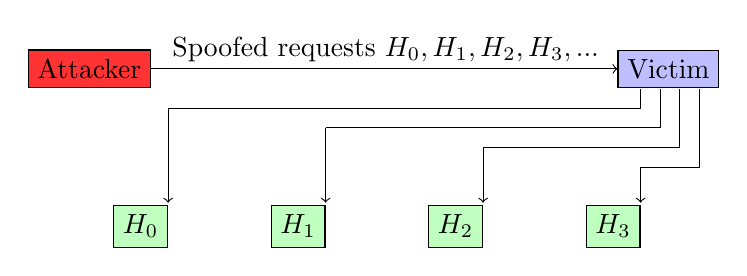
\begin{tikzpicture}{scale=0.4}
    \node[rectangle,draw,fill=red!80] (a) at (0,0) {Attacker};
    \node[anchor=west] at (0.93,0.25) {Spoofed requests $H_{0},H_{1},H_{2},H_{3},...$};
    \node [rectangle,draw,fill=blue!25,anchor=east] at (8,0) (v) {Victim};
    \draw [->](a) --(v);

    \foreach \x in {0,1,2,3} {
        \node [rectangle,draw,fill=green!25,anchor=east] at (\x*2+1,-2) {$H_{\x}$};
        %Horizontal lines
        \draw (\x*2+1, -\x*0.25-0.5)--(7.0+\x*.25,-\x*0.25-0.5);
        %Links to the victim
        \draw (7.0+\x*.25,-\x*0.25-0.5) -- (7.0+\x*.25,-0.25);
        %Links to hosts
        \draw[->] (\x*2+1, -\x*0.25-0.5)--(\x*2+1,-1.70);
    }
    \end{tikzpicture}


\begin{center}
    \begin{tabular}{|l|}
        \hline
        Connections\\
        \hline
        $H_{0}$\\
        \hline
        $H_{1}$\\
        \hline
        $H_{2}$\\
        \hline
        $H_{3}$\\
        \hline
    \end{tabular}
\end{center}

\begin{center}
Fill up state connection state table of the victim
\end{center}

\end{frame}

\begin{frame}
\frametitle{How does backscatter look like?}
\lstset{%                                                                       
  backgroundcolor=\color{gray!25},                                              
  basicstyle=\ttfamily,                                                         
  breaklines=true,                                                              
  columns=fullflexible                                                          
} 
\begin{lstlisting}
2017-09-16 10:02:22.807286 IP x.45.177.71.80 > x.x.105.167.39468: Flags [.], ack 1562196897, win 16384, length 0
2017-09-16 10:02:27.514922 IP x.45.177.71.80 > x.x.121.213.62562: Flags [.], ack 14588990, win 16384, length 0
2017-09-16 10:02:28.024516 IP x.45.177.71.80 > x.x.100.72.30395: Flags [.], ack 24579479, win 16384, length 0
2017-09-16 10:02:30.356876 IP x.45.177.71.80 > x.x.65.254.17754: Flags [.], ack 318490736, win 16384, length 0
\end{lstlisting}

\begin{center}
    \alert{What are the typical characteristics?}
\end{center}
\end{frame}

\begin{frame}
\frametitle{What can be derived from backscatter traffic?}

\begin{itemize}
    \item External point of view on ongoing denial of service attacks
    \item Confirm if there is a DDOS attack
    \item Recover time line of attacked targets
    \item Confirm which services (DNS, webserver, $\dots$)
    \item Infrastructure changes
    \item Assess the state of an infrastructure under denial of service attack
    \begin{itemize}
        \item Detect failure/addition of  intermediate network equipments, firewalls, proxy servers etc
        \item Detect DDoS mitigation devices
    \end{itemize}
    \item Create probabilistic models of denial of service attacks
\end{itemize}
\end{frame}

\begin{frame}
    \frametitle{Confirm if there is a DDOS attack}
    \begin{block}{Problem}
        \begin{itemize}
            \item Distinguish between compromised infrastructure and backscatter
            \item Look at TCP flags $\to$ filter out single SYN flags
            \item Focus on ACK, SYN/ACK, ...
            \item Do not limit to SYN/ACK or ACK $\to$ ECE (ECN Echo)\footnote{\url{https://tools.ietf.org/html/rfc3168}}
        \end{itemize}
    \end{block}
    \lstset{%
    backgroundcolor=\color{gray!25},
    basicstyle=\ttfamily,
    breaklines=true,
    columns=fullflexible
}

\begin{lstlisting}
tshark -n -r  capture-20170916110006.cap.gz -T fields -e frame.time_epoch  -e ip.src -e tcp.flags
1505552542.807286000 x.45.177.71 0x00000010
1505552547.514922000 x.45.177.71 0x00000010
\end{lstlisting}

\end{frame}

\begin{frame}
    \frametitle{Backscatter traffic evolution}
    \begin{center}
        \scalebox{0.9}{% GNUPLOT: LaTeX picture
\setlength{\unitlength}{0.240900pt}
\ifx\plotpoint\undefined\newsavebox{\plotpoint}\fi
\sbox{\plotpoint}{\rule[-0.200pt]{0.400pt}{0.400pt}}%
\begin{picture}(1500,900)(0,0)
\sbox{\plotpoint}{\rule[-0.200pt]{0.400pt}{0.400pt}}%
\put(231.0,190.0){\rule[-0.200pt]{291.007pt}{0.400pt}}
\put(231.0,190.0){\rule[-0.200pt]{4.818pt}{0.400pt}}
\put(211,190){\makebox(0,0)[r]{$0$}}
\put(1419.0,190.0){\rule[-0.200pt]{4.818pt}{0.400pt}}
\put(231.0,288.0){\rule[-0.200pt]{291.007pt}{0.400pt}}
\put(231.0,288.0){\rule[-0.200pt]{4.818pt}{0.400pt}}
\put(211,288){\makebox(0,0)[r]{$500000$}}
\put(1419.0,288.0){\rule[-0.200pt]{4.818pt}{0.400pt}}
\put(231.0,385.0){\rule[-0.200pt]{291.007pt}{0.400pt}}
\put(231.0,385.0){\rule[-0.200pt]{4.818pt}{0.400pt}}
\put(211,385){\makebox(0,0)[r]{$1\times10^{6}$}}
\put(1419.0,385.0){\rule[-0.200pt]{4.818pt}{0.400pt}}
\put(231.0,483.0){\rule[-0.200pt]{291.007pt}{0.400pt}}
\put(231.0,483.0){\rule[-0.200pt]{4.818pt}{0.400pt}}
\put(211,483){\makebox(0,0)[r]{$1.5\times10^{6}$}}
\put(1419.0,483.0){\rule[-0.200pt]{4.818pt}{0.400pt}}
\put(231.0,581.0){\rule[-0.200pt]{291.007pt}{0.400pt}}
\put(231.0,581.0){\rule[-0.200pt]{4.818pt}{0.400pt}}
\put(211,581){\makebox(0,0)[r]{$2\times10^{6}$}}
\put(1419.0,581.0){\rule[-0.200pt]{4.818pt}{0.400pt}}
\put(231.0,678.0){\rule[-0.200pt]{199.465pt}{0.400pt}}
\put(1419.0,678.0){\rule[-0.200pt]{4.818pt}{0.400pt}}
\put(231.0,678.0){\rule[-0.200pt]{4.818pt}{0.400pt}}
\put(211,678){\makebox(0,0)[r]{$2.5\times10^{6}$}}
\put(1419.0,678.0){\rule[-0.200pt]{4.818pt}{0.400pt}}
\put(231.0,776.0){\rule[-0.200pt]{291.007pt}{0.400pt}}
\put(231.0,776.0){\rule[-0.200pt]{4.818pt}{0.400pt}}
\put(211,776){\makebox(0,0)[r]{$3\times10^{6}$}}
\put(1419.0,776.0){\rule[-0.200pt]{4.818pt}{0.400pt}}
\put(262.0,190.0){\rule[-0.200pt]{0.400pt}{2.409pt}}
\put(372.0,190.0){\rule[-0.200pt]{0.400pt}{141.167pt}}
\put(372,170){\makebox(0,0)[l]{01/10}}
\put(372.0,190.0){\rule[-0.200pt]{0.400pt}{4.818pt}}
\put(482.0,190.0){\rule[-0.200pt]{0.400pt}{2.409pt}}
\put(592.0,190.0){\rule[-0.200pt]{0.400pt}{141.167pt}}
\put(592,170){\makebox(0,0)[l]{01/24}}
\put(592.0,190.0){\rule[-0.200pt]{0.400pt}{4.818pt}}
\put(702.0,190.0){\rule[-0.200pt]{0.400pt}{2.409pt}}
\put(811.0,190.0){\rule[-0.200pt]{0.400pt}{141.167pt}}
\put(811,170){\makebox(0,0)[l]{02/07}}
\put(811.0,190.0){\rule[-0.200pt]{0.400pt}{4.818pt}}
\put(921.0,190.0){\rule[-0.200pt]{0.400pt}{2.409pt}}
\put(1031.0,190.0){\rule[-0.200pt]{0.400pt}{141.167pt}}
\put(1031,170){\makebox(0,0)[l]{02/21}}
\put(1031.0,190.0){\rule[-0.200pt]{0.400pt}{4.818pt}}
\put(1141.0,190.0){\rule[-0.200pt]{0.400pt}{2.409pt}}
\put(1251.0,190.0){\rule[-0.200pt]{0.400pt}{116.596pt}}
\put(1251.0,756.0){\rule[-0.200pt]{0.400pt}{4.818pt}}
\put(1251,170){\makebox(0,0)[l]{03/07}}
\put(1251.0,190.0){\rule[-0.200pt]{0.400pt}{4.818pt}}
\put(1361.0,190.0){\rule[-0.200pt]{0.400pt}{2.409pt}}
\put(231.0,190.0){\rule[-0.200pt]{0.400pt}{141.167pt}}
\put(231.0,190.0){\rule[-0.200pt]{291.007pt}{0.400pt}}
\put(1439.0,190.0){\rule[-0.200pt]{0.400pt}{141.167pt}}
\put(231.0,776.0){\rule[-0.200pt]{291.007pt}{0.400pt}}
\put(261,747){\makebox(0,0)[l]{https://www.circl.lu/}}
\put(30,483){\makebox(0,0){Number of packets}}
\put(835,29){\makebox(0,0){date (month / day)}}
\put(835,838){\makebox(0,0){Backscatter traffic volume per 5 minutes in 2019}}
\put(1279,735){\makebox(0,0)[r]{backscatter}}
\put(1299.0,735.0){\rule[-0.200pt]{24.090pt}{0.400pt}}
\put(231,195){\usebox{\plotpoint}}
\put(231.0,195.0){\rule[-0.200pt]{0.400pt}{0.482pt}}
\put(231,194.67){\rule{0.241pt}{0.400pt}}
\multiput(231.00,194.17)(0.500,1.000){2}{\rule{0.120pt}{0.400pt}}
\put(231.0,195.0){\rule[-0.200pt]{0.400pt}{0.482pt}}
\put(232,196){\usebox{\plotpoint}}
\put(232.0,195.0){\usebox{\plotpoint}}
\put(232.0,195.0){\usebox{\plotpoint}}
\put(232.0,195.0){\usebox{\plotpoint}}
\put(232.0,195.0){\usebox{\plotpoint}}
\put(232.0,195.0){\usebox{\plotpoint}}
\put(232.0,195.0){\usebox{\plotpoint}}
\put(232.0,195.0){\usebox{\plotpoint}}
\put(232.0,195.0){\rule[-0.200pt]{0.400pt}{0.482pt}}
\put(232.0,195.0){\rule[-0.200pt]{0.400pt}{0.482pt}}
\put(232.0,195.0){\usebox{\plotpoint}}
\put(232.0,196.0){\usebox{\plotpoint}}
\put(233.0,196.0){\usebox{\plotpoint}}
\put(233.0,196.0){\usebox{\plotpoint}}
\put(233.0,196.0){\rule[-0.200pt]{0.400pt}{0.482pt}}
\put(233.0,196.0){\rule[-0.200pt]{0.400pt}{0.482pt}}
\put(233.0,196.0){\rule[-0.200pt]{0.400pt}{0.723pt}}
\put(233.0,198.0){\usebox{\plotpoint}}
\put(233,198.67){\rule{0.241pt}{0.400pt}}
\multiput(233.00,199.17)(0.500,-1.000){2}{\rule{0.120pt}{0.400pt}}
\put(233.0,198.0){\rule[-0.200pt]{0.400pt}{0.482pt}}
\put(234.0,199.0){\rule[-0.200pt]{0.400pt}{0.482pt}}
\put(234.0,199.0){\rule[-0.200pt]{0.400pt}{0.482pt}}
\put(234.0,199.0){\rule[-0.200pt]{0.400pt}{0.723pt}}
\put(234.0,201.0){\usebox{\plotpoint}}
\put(234.0,201.0){\rule[-0.200pt]{0.400pt}{0.482pt}}
\put(234.0,201.0){\rule[-0.200pt]{0.400pt}{0.482pt}}
\put(234,201.67){\rule{0.241pt}{0.400pt}}
\multiput(234.00,202.17)(0.500,-1.000){2}{\rule{0.120pt}{0.400pt}}
\put(234.0,201.0){\rule[-0.200pt]{0.400pt}{0.482pt}}
\put(235.0,202.0){\rule[-0.200pt]{0.400pt}{1.445pt}}
\put(235.0,204.0){\rule[-0.200pt]{0.400pt}{0.964pt}}
\put(235.0,204.0){\usebox{\plotpoint}}
\put(235.0,203.0){\rule[-0.200pt]{0.400pt}{0.482pt}}
\put(235.0,203.0){\usebox{\plotpoint}}
\put(235.0,203.0){\usebox{\plotpoint}}
\put(235,202.67){\rule{0.241pt}{0.400pt}}
\multiput(235.00,203.17)(0.500,-1.000){2}{\rule{0.120pt}{0.400pt}}
\put(235.0,203.0){\usebox{\plotpoint}}
\put(236,203){\usebox{\plotpoint}}
\put(236,203){\usebox{\plotpoint}}
\put(236.0,202.0){\usebox{\plotpoint}}
\put(236.0,202.0){\rule[-0.200pt]{0.400pt}{0.482pt}}
\put(236.0,203.0){\usebox{\plotpoint}}
\put(236.0,203.0){\rule[-0.200pt]{0.400pt}{0.482pt}}
\put(236,203.67){\rule{0.241pt}{0.400pt}}
\multiput(236.00,203.17)(0.500,1.000){2}{\rule{0.120pt}{0.400pt}}
\put(236.0,204.0){\usebox{\plotpoint}}
\put(237.0,204.0){\usebox{\plotpoint}}
\put(237.0,204.0){\usebox{\plotpoint}}
\put(237.0,203.0){\rule[-0.200pt]{0.400pt}{0.482pt}}
\put(237.0,203.0){\rule[-0.200pt]{0.400pt}{0.723pt}}
\put(237.0,204.0){\rule[-0.200pt]{0.400pt}{0.482pt}}
\put(237.0,204.0){\usebox{\plotpoint}}
\put(237.0,204.0){\usebox{\plotpoint}}
\put(237.0,204.0){\rule[-0.200pt]{0.400pt}{0.482pt}}
\put(237.0,205.0){\usebox{\plotpoint}}
\put(237.0,205.0){\usebox{\plotpoint}}
\put(237.0,204.0){\rule[-0.200pt]{0.400pt}{0.482pt}}
\put(237.0,204.0){\usebox{\plotpoint}}
\put(238.0,203.0){\usebox{\plotpoint}}
\put(238.0,203.0){\usebox{\plotpoint}}
\put(238.0,203.0){\usebox{\plotpoint}}
\put(238.0,203.0){\rule[-0.200pt]{0.400pt}{0.482pt}}
\put(238.0,202.0){\rule[-0.200pt]{0.400pt}{0.723pt}}
\put(238.0,202.0){\usebox{\plotpoint}}
\put(238.0,202.0){\usebox{\plotpoint}}
\put(238.0,202.0){\usebox{\plotpoint}}
\put(239.0,202.0){\usebox{\plotpoint}}
\put(239.0,201.0){\rule[-0.200pt]{0.400pt}{0.482pt}}
\put(239.0,201.0){\rule[-0.200pt]{0.400pt}{1.204pt}}
\put(239,204.67){\rule{0.241pt}{0.400pt}}
\multiput(239.00,204.17)(0.500,1.000){2}{\rule{0.120pt}{0.400pt}}
\put(239.0,205.0){\usebox{\plotpoint}}
\put(240.0,205.0){\usebox{\plotpoint}}
\put(240.0,205.0){\rule[-0.200pt]{0.400pt}{0.723pt}}
\put(240.0,201.0){\rule[-0.200pt]{0.400pt}{1.686pt}}
\put(240.0,201.0){\rule[-0.200pt]{0.400pt}{0.723pt}}
\put(240.0,202.0){\rule[-0.200pt]{0.400pt}{0.482pt}}
\put(240.0,202.0){\rule[-0.200pt]{0.400pt}{0.482pt}}
\put(240.0,202.0){\rule[-0.200pt]{0.400pt}{0.482pt}}
\put(240,202.67){\rule{0.241pt}{0.400pt}}
\multiput(240.00,202.17)(0.500,1.000){2}{\rule{0.120pt}{0.400pt}}
\put(240.0,202.0){\usebox{\plotpoint}}
\put(241.0,204.0){\usebox{\plotpoint}}
\put(241.0,202.0){\rule[-0.200pt]{0.400pt}{0.723pt}}
\put(241.0,202.0){\usebox{\plotpoint}}
\put(241.0,202.0){\usebox{\plotpoint}}
\put(241.0,202.0){\rule[-0.200pt]{0.400pt}{0.482pt}}
\put(241.0,203.0){\usebox{\plotpoint}}
\put(241.0,203.0){\usebox{\plotpoint}}
\put(241,202.67){\rule{0.241pt}{0.400pt}}
\multiput(241.00,202.17)(0.500,1.000){2}{\rule{0.120pt}{0.400pt}}
\put(241.0,203.0){\usebox{\plotpoint}}
\put(242,204){\usebox{\plotpoint}}
\put(242,204){\usebox{\plotpoint}}
\put(242,204){\usebox{\plotpoint}}
\put(242,204){\usebox{\plotpoint}}
\put(242,204){\usebox{\plotpoint}}
\put(242,204){\usebox{\plotpoint}}
\put(242,204){\usebox{\plotpoint}}
\put(242,204){\usebox{\plotpoint}}
\put(242,204){\usebox{\plotpoint}}
\put(242,204){\usebox{\plotpoint}}
\put(242.0,204.0){\usebox{\plotpoint}}
\put(242.0,203.0){\rule[-0.200pt]{0.400pt}{0.482pt}}
\put(242,203.67){\rule{0.241pt}{0.400pt}}
\multiput(242.00,204.17)(0.500,-1.000){2}{\rule{0.120pt}{0.400pt}}
\put(242.0,203.0){\rule[-0.200pt]{0.400pt}{0.482pt}}
\put(243,204){\usebox{\plotpoint}}
\put(243,204){\usebox{\plotpoint}}
\put(243,204){\usebox{\plotpoint}}
\put(243,204){\usebox{\plotpoint}}
\put(243,204){\usebox{\plotpoint}}
\put(243,204){\usebox{\plotpoint}}
\put(243,204){\usebox{\plotpoint}}
\put(243,204){\usebox{\plotpoint}}
\put(243,204){\usebox{\plotpoint}}
\put(243,204){\usebox{\plotpoint}}
\put(243,204){\usebox{\plotpoint}}
\put(243.0,203.0){\usebox{\plotpoint}}
\put(243.0,203.0){\usebox{\plotpoint}}
\put(244.0,201.0){\rule[-0.200pt]{0.400pt}{0.482pt}}
\put(244.0,201.0){\rule[-0.200pt]{0.400pt}{0.482pt}}
\put(243.67,197){\rule{0.400pt}{0.482pt}}
\multiput(243.17,197.00)(1.000,1.000){2}{\rule{0.400pt}{0.241pt}}
\put(244.0,197.0){\rule[-0.200pt]{0.400pt}{1.445pt}}
\put(245.0,195.0){\rule[-0.200pt]{0.400pt}{0.964pt}}
\put(245,194.67){\rule{0.241pt}{0.400pt}}
\multiput(245.00,195.17)(0.500,-1.000){2}{\rule{0.120pt}{0.400pt}}
\put(245.0,195.0){\usebox{\plotpoint}}
\put(246,195){\usebox{\plotpoint}}
\put(246,195){\usebox{\plotpoint}}
\put(246,195){\usebox{\plotpoint}}
\put(246,195){\usebox{\plotpoint}}
\put(246,195){\usebox{\plotpoint}}
\put(246,195){\usebox{\plotpoint}}
\put(246,195){\usebox{\plotpoint}}
\put(246,195){\usebox{\plotpoint}}
\put(246.0,195.0){\usebox{\plotpoint}}
\put(246.0,194.0){\rule[-0.200pt]{0.400pt}{0.482pt}}
\put(245.67,195){\rule{0.400pt}{0.482pt}}
\multiput(245.17,195.00)(1.000,1.000){2}{\rule{0.400pt}{0.241pt}}
\put(246.0,194.0){\usebox{\plotpoint}}
\put(247.0,195.0){\rule[-0.200pt]{0.400pt}{0.482pt}}
\put(247.0,195.0){\usebox{\plotpoint}}
\put(247.0,195.0){\usebox{\plotpoint}}
\put(247.0,195.0){\usebox{\plotpoint}}
\put(247.0,195.0){\usebox{\plotpoint}}
\put(247.0,195.0){\usebox{\plotpoint}}
\put(247.0,195.0){\usebox{\plotpoint}}
\put(247,195.67){\rule{0.241pt}{0.400pt}}
\multiput(247.00,196.17)(0.500,-1.000){2}{\rule{0.120pt}{0.400pt}}
\put(247.0,195.0){\rule[-0.200pt]{0.400pt}{0.482pt}}
\put(248,196){\usebox{\plotpoint}}
\put(248,196){\usebox{\plotpoint}}
\put(248,196){\usebox{\plotpoint}}
\put(248.0,196.0){\rule[-0.200pt]{0.400pt}{0.482pt}}
\put(248.0,196.0){\rule[-0.200pt]{0.400pt}{0.482pt}}
\put(248.0,196.0){\rule[-0.200pt]{0.400pt}{0.723pt}}
\put(248.0,196.0){\rule[-0.200pt]{0.400pt}{0.723pt}}
\put(248.0,196.0){\rule[-0.200pt]{0.400pt}{0.482pt}}
\put(248.0,197.0){\usebox{\plotpoint}}
\put(248.0,197.0){\usebox{\plotpoint}}
\put(249.0,197.0){\usebox{\plotpoint}}
\put(249.0,197.0){\usebox{\plotpoint}}
\put(249.0,197.0){\rule[-0.200pt]{0.400pt}{0.723pt}}
\put(249.0,199.0){\usebox{\plotpoint}}
\put(249.0,199.0){\rule[-0.200pt]{0.400pt}{0.723pt}}
\put(249,197.67){\rule{0.241pt}{0.400pt}}
\multiput(249.00,197.17)(0.500,1.000){2}{\rule{0.120pt}{0.400pt}}
\put(249.0,198.0){\rule[-0.200pt]{0.400pt}{0.964pt}}
\put(250,199){\usebox{\plotpoint}}
\put(250.0,199.0){\rule[-0.200pt]{0.400pt}{0.482pt}}
\put(250.0,200.0){\usebox{\plotpoint}}
\put(250.0,200.0){\usebox{\plotpoint}}
\put(250.0,199.0){\rule[-0.200pt]{0.400pt}{0.482pt}}
\put(250.0,199.0){\rule[-0.200pt]{0.400pt}{0.482pt}}
\put(250.0,199.0){\rule[-0.200pt]{0.400pt}{0.482pt}}
\put(250.0,199.0){\rule[-0.200pt]{0.400pt}{1.445pt}}
\put(250.0,201.0){\rule[-0.200pt]{0.400pt}{0.964pt}}
\put(250.0,201.0){\rule[-0.200pt]{0.400pt}{0.482pt}}
\put(250.0,202.0){\usebox{\plotpoint}}
\put(250.0,202.0){\rule[-0.200pt]{0.400pt}{0.482pt}}
\put(250.0,202.0){\rule[-0.200pt]{0.400pt}{0.482pt}}
\put(250.0,202.0){\usebox{\plotpoint}}
\put(251.0,201.0){\usebox{\plotpoint}}
\put(251.0,201.0){\usebox{\plotpoint}}
\put(251.0,200.0){\rule[-0.200pt]{0.400pt}{0.482pt}}
\put(251.0,200.0){\usebox{\plotpoint}}
\put(251.0,200.0){\usebox{\plotpoint}}
\put(251.0,200.0){\usebox{\plotpoint}}
\put(251.0,200.0){\usebox{\plotpoint}}
\put(251.0,200.0){\usebox{\plotpoint}}
\put(251.0,200.0){\usebox{\plotpoint}}
\put(251.0,200.0){\usebox{\plotpoint}}
\put(252.0,200.0){\rule[-0.200pt]{0.400pt}{0.723pt}}
\put(252.0,201.0){\rule[-0.200pt]{0.400pt}{0.482pt}}
\put(252.0,201.0){\rule[-0.200pt]{0.400pt}{0.964pt}}
\put(252.0,200.0){\rule[-0.200pt]{0.400pt}{1.204pt}}
\put(252.0,200.0){\rule[-0.200pt]{0.400pt}{0.482pt}}
\put(252.0,201.0){\usebox{\plotpoint}}
\put(252.0,201.0){\usebox{\plotpoint}}
\put(253.0,201.0){\usebox{\plotpoint}}
\put(253.0,201.0){\usebox{\plotpoint}}
\put(253.0,201.0){\usebox{\plotpoint}}
\put(253.0,201.0){\usebox{\plotpoint}}
\put(253.0,201.0){\usebox{\plotpoint}}
\put(253.0,201.0){\usebox{\plotpoint}}
\put(253.0,201.0){\usebox{\plotpoint}}
\put(254.0,201.0){\rule[-0.200pt]{0.400pt}{0.482pt}}
\put(254.0,201.0){\rule[-0.200pt]{0.400pt}{0.482pt}}
\put(254.0,201.0){\usebox{\plotpoint}}
\put(254,199.67){\rule{0.241pt}{0.400pt}}
\multiput(254.00,200.17)(0.500,-1.000){2}{\rule{0.120pt}{0.400pt}}
\put(254.0,201.0){\usebox{\plotpoint}}
\put(255.0,200.0){\rule[-0.200pt]{0.400pt}{0.723pt}}
\put(255.0,202.0){\usebox{\plotpoint}}
\put(255.0,202.0){\usebox{\plotpoint}}
\put(255.0,201.0){\rule[-0.200pt]{0.400pt}{0.482pt}}
\put(255.0,201.0){\usebox{\plotpoint}}
\put(255.0,201.0){\usebox{\plotpoint}}
\put(255.0,201.0){\usebox{\plotpoint}}
\put(255.0,201.0){\usebox{\plotpoint}}
\put(255.0,201.0){\rule[-0.200pt]{0.400pt}{0.964pt}}
\put(255.0,202.0){\rule[-0.200pt]{0.400pt}{0.723pt}}
\put(255.0,202.0){\usebox{\plotpoint}}
\put(256.0,200.0){\rule[-0.200pt]{0.400pt}{0.482pt}}
\put(256.0,200.0){\rule[-0.200pt]{0.400pt}{0.723pt}}
\put(256.0,200.0){\rule[-0.200pt]{0.400pt}{0.723pt}}
\put(256.0,200.0){\rule[-0.200pt]{0.400pt}{1.686pt}}
\put(256.0,202.0){\rule[-0.200pt]{0.400pt}{1.204pt}}
\put(256.0,202.0){\usebox{\plotpoint}}
\put(256.0,203.0){\usebox{\plotpoint}}
\put(257.0,203.0){\rule[-0.200pt]{0.400pt}{0.482pt}}
\put(257.0,202.0){\rule[-0.200pt]{0.400pt}{0.723pt}}
\put(257.0,202.0){\usebox{\plotpoint}}
\put(257.0,202.0){\usebox{\plotpoint}}
\put(257.0,202.0){\usebox{\plotpoint}}
\put(258.0,202.0){\rule[-0.200pt]{0.400pt}{0.482pt}}
\put(258.0,203.0){\usebox{\plotpoint}}
\put(258.0,203.0){\rule[-0.200pt]{0.400pt}{0.482pt}}
\put(258,202.67){\rule{0.241pt}{0.400pt}}
\multiput(258.00,203.17)(0.500,-1.000){2}{\rule{0.120pt}{0.400pt}}
\put(258.0,204.0){\usebox{\plotpoint}}
\put(259.0,203.0){\usebox{\plotpoint}}
\put(259.0,203.0){\usebox{\plotpoint}}
\put(259.0,203.0){\usebox{\plotpoint}}
\put(259.0,202.0){\rule[-0.200pt]{0.400pt}{0.482pt}}
\put(259.0,202.0){\usebox{\plotpoint}}
\put(259.0,201.0){\rule[-0.200pt]{0.400pt}{0.482pt}}
\put(258.67,200){\rule{0.400pt}{0.482pt}}
\multiput(258.17,201.00)(1.000,-1.000){2}{\rule{0.400pt}{0.241pt}}
\put(259.0,201.0){\usebox{\plotpoint}}
\put(260,200){\usebox{\plotpoint}}
\put(260.0,198.0){\rule[-0.200pt]{0.400pt}{0.482pt}}
\put(260.0,198.0){\usebox{\plotpoint}}
\put(260.0,195.0){\rule[-0.200pt]{0.400pt}{0.964pt}}
\put(260.0,195.0){\usebox{\plotpoint}}
\put(261.0,194.0){\usebox{\plotpoint}}
\put(261.0,194.0){\usebox{\plotpoint}}
\put(261.0,194.0){\usebox{\plotpoint}}
\put(261.0,194.0){\usebox{\plotpoint}}
\put(261.0,194.0){\usebox{\plotpoint}}
\put(261.0,194.0){\usebox{\plotpoint}}
\put(261.0,195.0){\usebox{\plotpoint}}
\put(262.0,194.0){\usebox{\plotpoint}}
\put(262.0,194.0){\usebox{\plotpoint}}
\put(262.0,193.0){\rule[-0.200pt]{0.400pt}{0.482pt}}
\put(262.0,193.0){\rule[-0.200pt]{0.400pt}{0.482pt}}
\put(262.0,194.0){\usebox{\plotpoint}}
\put(262.0,194.0){\usebox{\plotpoint}}
\put(263.0,194.0){\usebox{\plotpoint}}
\put(263.0,194.0){\usebox{\plotpoint}}
\put(263.0,194.0){\usebox{\plotpoint}}
\put(263.0,194.0){\usebox{\plotpoint}}
\put(263.0,194.0){\rule[-0.200pt]{0.400pt}{0.482pt}}
\put(263.0,194.0){\rule[-0.200pt]{0.400pt}{0.482pt}}
\put(263.0,194.0){\rule[-0.200pt]{0.400pt}{0.482pt}}
\put(263.0,195.0){\usebox{\plotpoint}}
\put(263.0,195.0){\usebox{\plotpoint}}
\put(264.0,195.0){\rule[-0.200pt]{0.400pt}{0.482pt}}
\put(264.0,196.0){\usebox{\plotpoint}}
\put(264.0,196.0){\usebox{\plotpoint}}
\put(264.0,195.0){\rule[-0.200pt]{0.400pt}{0.482pt}}
\put(264.0,195.0){\rule[-0.200pt]{0.400pt}{0.482pt}}
\put(264.0,196.0){\usebox{\plotpoint}}
\put(264.0,196.0){\usebox{\plotpoint}}
\put(264.0,196.0){\usebox{\plotpoint}}
\put(264.0,196.0){\rule[-0.200pt]{0.400pt}{0.482pt}}
\put(264.0,197.0){\usebox{\plotpoint}}
\put(264.0,197.0){\usebox{\plotpoint}}
\put(265.0,197.0){\rule[-0.200pt]{0.400pt}{0.482pt}}
\put(265.0,198.0){\usebox{\plotpoint}}
\put(265.0,198.0){\usebox{\plotpoint}}
\put(265.0,198.0){\usebox{\plotpoint}}
\put(265.0,198.0){\usebox{\plotpoint}}
\put(265.0,198.0){\usebox{\plotpoint}}
\put(265.0,198.0){\rule[-0.200pt]{0.400pt}{0.482pt}}
\put(265.0,199.0){\usebox{\plotpoint}}
\put(265.0,199.0){\rule[-0.200pt]{0.400pt}{0.723pt}}
\put(265.0,201.0){\usebox{\plotpoint}}
\put(265,200.67){\rule{0.241pt}{0.400pt}}
\multiput(265.00,201.17)(0.500,-1.000){2}{\rule{0.120pt}{0.400pt}}
\put(265.0,201.0){\usebox{\plotpoint}}
\put(266,201){\usebox{\plotpoint}}
\put(266.0,200.0){\usebox{\plotpoint}}
\put(266.0,200.0){\rule[-0.200pt]{0.400pt}{0.723pt}}
\put(266.0,200.0){\rule[-0.200pt]{0.400pt}{0.723pt}}
\put(266,200.67){\rule{0.241pt}{0.400pt}}
\multiput(266.00,200.17)(0.500,1.000){2}{\rule{0.120pt}{0.400pt}}
\put(266.0,200.0){\usebox{\plotpoint}}
\put(267.0,200.0){\rule[-0.200pt]{0.400pt}{0.482pt}}
\put(267.0,200.0){\rule[-0.200pt]{0.400pt}{0.723pt}}
\put(267.0,201.0){\rule[-0.200pt]{0.400pt}{0.482pt}}
\put(267.0,201.0){\rule[-0.200pt]{0.400pt}{1.204pt}}
\put(267.0,202.0){\rule[-0.200pt]{0.400pt}{0.964pt}}
\put(267.0,202.0){\usebox{\plotpoint}}
\put(267.0,202.0){\usebox{\plotpoint}}
\put(267.0,202.0){\usebox{\plotpoint}}
\put(267,200.67){\rule{0.241pt}{0.400pt}}
\multiput(267.00,201.17)(0.500,-1.000){2}{\rule{0.120pt}{0.400pt}}
\put(267.0,202.0){\usebox{\plotpoint}}
\put(268,201){\usebox{\plotpoint}}
\put(268,201){\usebox{\plotpoint}}
\put(268.0,201.0){\rule[-0.200pt]{0.400pt}{0.482pt}}
\put(268.0,200.0){\rule[-0.200pt]{0.400pt}{0.723pt}}
\put(268.0,200.0){\rule[-0.200pt]{0.400pt}{2.650pt}}
\put(268.0,202.0){\rule[-0.200pt]{0.400pt}{2.168pt}}
\put(268.0,202.0){\rule[-0.200pt]{0.400pt}{1.204pt}}
\put(268.0,201.0){\rule[-0.200pt]{0.400pt}{1.445pt}}
\put(268.0,201.0){\usebox{\plotpoint}}
\put(269.0,201.0){\usebox{\plotpoint}}
\put(269.0,201.0){\usebox{\plotpoint}}
\put(269.0,201.0){\usebox{\plotpoint}}
\put(269.0,201.0){\usebox{\plotpoint}}
\put(269.0,201.0){\usebox{\plotpoint}}
\put(269.0,201.0){\usebox{\plotpoint}}
\put(269.0,201.0){\usebox{\plotpoint}}
\put(269.0,201.0){\usebox{\plotpoint}}
\put(269.0,201.0){\usebox{\plotpoint}}
\put(269.0,201.0){\usebox{\plotpoint}}
\put(269.0,201.0){\usebox{\plotpoint}}
\put(270.0,200.0){\usebox{\plotpoint}}
\put(270.0,200.0){\rule[-0.200pt]{0.400pt}{0.482pt}}
\put(270.0,201.0){\usebox{\plotpoint}}
\put(270.0,201.0){\rule[-0.200pt]{0.400pt}{0.723pt}}
\put(270.0,201.0){\rule[-0.200pt]{0.400pt}{0.723pt}}
\put(270.0,201.0){\usebox{\plotpoint}}
\put(270.0,201.0){\usebox{\plotpoint}}
\put(270.0,201.0){\usebox{\plotpoint}}
\put(271.0,200.0){\usebox{\plotpoint}}
\put(271.0,200.0){\usebox{\plotpoint}}
\put(271.0,200.0){\usebox{\plotpoint}}
\put(271.0,200.0){\rule[-0.200pt]{0.400pt}{0.482pt}}
\put(271,199.67){\rule{0.241pt}{0.400pt}}
\multiput(271.00,199.17)(0.500,1.000){2}{\rule{0.120pt}{0.400pt}}
\put(271.0,200.0){\rule[-0.200pt]{0.400pt}{0.482pt}}
\put(272,201){\usebox{\plotpoint}}
\put(272.0,200.0){\usebox{\plotpoint}}
\put(272.0,200.0){\usebox{\plotpoint}}
\put(272.0,200.0){\usebox{\plotpoint}}
\put(272.0,200.0){\usebox{\plotpoint}}
\put(272.0,200.0){\usebox{\plotpoint}}
\put(272.0,200.0){\rule[-0.200pt]{0.400pt}{0.964pt}}
\put(272.0,202.0){\rule[-0.200pt]{0.400pt}{0.482pt}}
\put(272.0,202.0){\usebox{\plotpoint}}
\put(272.0,201.0){\rule[-0.200pt]{0.400pt}{0.482pt}}
\put(272.0,201.0){\usebox{\plotpoint}}
\put(273.0,201.0){\rule[-0.200pt]{0.400pt}{0.723pt}}
\put(273.0,203.0){\usebox{\plotpoint}}
\put(273.0,203.0){\usebox{\plotpoint}}
\put(273.0,203.0){\usebox{\plotpoint}}
\put(273.0,203.0){\rule[-0.200pt]{0.400pt}{0.723pt}}
\put(273.0,205.0){\usebox{\plotpoint}}
\put(273.0,205.0){\usebox{\plotpoint}}
\put(274.0,205.0){\usebox{\plotpoint}}
\put(274.0,205.0){\usebox{\plotpoint}}
\put(274.0,205.0){\usebox{\plotpoint}}
\put(274.0,205.0){\usebox{\plotpoint}}
\put(274,204.67){\rule{0.241pt}{0.400pt}}
\multiput(274.00,205.17)(0.500,-1.000){2}{\rule{0.120pt}{0.400pt}}
\put(274.0,205.0){\usebox{\plotpoint}}
\put(275,205){\usebox{\plotpoint}}
\put(275,205){\usebox{\plotpoint}}
\put(275,205){\usebox{\plotpoint}}
\put(275.0,203.0){\rule[-0.200pt]{0.400pt}{0.482pt}}
\put(275.0,203.0){\usebox{\plotpoint}}
\put(275.0,201.0){\rule[-0.200pt]{0.400pt}{0.723pt}}
\put(275.0,201.0){\rule[-0.200pt]{0.400pt}{0.964pt}}
\put(275.0,200.0){\rule[-0.200pt]{0.400pt}{1.204pt}}
\put(275.0,200.0){\usebox{\plotpoint}}
\put(276.0,197.0){\rule[-0.200pt]{0.400pt}{0.723pt}}
\put(276.0,197.0){\usebox{\plotpoint}}
\put(277.0,196.0){\usebox{\plotpoint}}
\put(277.0,196.0){\usebox{\plotpoint}}
\put(277.0,196.0){\usebox{\plotpoint}}
\put(277.0,196.0){\usebox{\plotpoint}}
\put(277.0,195.0){\rule[-0.200pt]{0.400pt}{0.482pt}}
\put(277.0,195.0){\usebox{\plotpoint}}
\put(277.0,196.0){\usebox{\plotpoint}}
\put(278.0,196.0){\rule[-0.200pt]{0.400pt}{0.482pt}}
\put(278.0,196.0){\rule[-0.200pt]{0.400pt}{0.482pt}}
\put(278.0,196.0){\rule[-0.200pt]{0.400pt}{0.482pt}}
\put(278.0,196.0){\rule[-0.200pt]{0.400pt}{0.482pt}}
\put(278.0,196.0){\usebox{\plotpoint}}
\put(278,195.67){\rule{0.241pt}{0.400pt}}
\multiput(278.00,195.17)(0.500,1.000){2}{\rule{0.120pt}{0.400pt}}
\put(278.0,196.0){\usebox{\plotpoint}}
\put(279.0,196.0){\usebox{\plotpoint}}
\put(279.0,196.0){\rule[-0.200pt]{0.400pt}{1.204pt}}
\put(279.0,197.0){\rule[-0.200pt]{0.400pt}{0.964pt}}
\put(279.0,197.0){\usebox{\plotpoint}}
\put(279.0,197.0){\usebox{\plotpoint}}
\put(279.0,197.0){\rule[-0.200pt]{0.400pt}{0.482pt}}
\put(279.0,197.0){\rule[-0.200pt]{0.400pt}{0.482pt}}
\put(279.0,197.0){\rule[-0.200pt]{0.400pt}{0.482pt}}
\put(279.0,198.0){\usebox{\plotpoint}}
\put(279.0,198.0){\usebox{\plotpoint}}
\put(280.0,198.0){\rule[-0.200pt]{0.400pt}{0.482pt}}
\put(280.0,198.0){\rule[-0.200pt]{0.400pt}{0.482pt}}
\put(280.0,198.0){\rule[-0.200pt]{0.400pt}{0.482pt}}
\put(280.0,199.0){\usebox{\plotpoint}}
\put(280.0,199.0){\usebox{\plotpoint}}
\put(280.0,198.0){\rule[-0.200pt]{0.400pt}{0.482pt}}
\put(280.0,198.0){\rule[-0.200pt]{0.400pt}{0.723pt}}
\put(280,198.67){\rule{0.241pt}{0.400pt}}
\multiput(280.00,198.17)(0.500,1.000){2}{\rule{0.120pt}{0.400pt}}
\put(280.0,199.0){\rule[-0.200pt]{0.400pt}{0.482pt}}
\put(281.0,200.0){\rule[-0.200pt]{0.400pt}{0.723pt}}
\put(281.0,201.0){\rule[-0.200pt]{0.400pt}{0.482pt}}
\put(281.0,201.0){\usebox{\plotpoint}}
\put(281.0,199.0){\rule[-0.200pt]{0.400pt}{0.723pt}}
\put(281.0,199.0){\usebox{\plotpoint}}
\put(281.0,199.0){\usebox{\plotpoint}}
\put(281.0,199.0){\rule[-0.200pt]{0.400pt}{0.482pt}}
\put(281.0,199.0){\rule[-0.200pt]{0.400pt}{0.482pt}}
\put(281.0,199.0){\rule[-0.200pt]{0.400pt}{0.482pt}}
\put(281.0,200.0){\usebox{\plotpoint}}
\put(281.0,200.0){\usebox{\plotpoint}}
\put(281,199.67){\rule{0.241pt}{0.400pt}}
\multiput(281.00,199.17)(0.500,1.000){2}{\rule{0.120pt}{0.400pt}}
\put(281.0,200.0){\usebox{\plotpoint}}
\put(282,201){\usebox{\plotpoint}}
\put(282.0,201.0){\rule[-0.200pt]{0.400pt}{0.723pt}}
\put(282.0,202.0){\rule[-0.200pt]{0.400pt}{0.482pt}}
\put(282.0,202.0){\rule[-0.200pt]{0.400pt}{0.482pt}}
\put(282.0,201.0){\rule[-0.200pt]{0.400pt}{0.723pt}}
\put(282.0,201.0){\rule[-0.200pt]{0.400pt}{0.964pt}}
\put(282.0,202.0){\rule[-0.200pt]{0.400pt}{0.723pt}}
\put(282.0,202.0){\usebox{\plotpoint}}
\put(283.0,202.0){\usebox{\plotpoint}}
\put(283.0,201.0){\rule[-0.200pt]{0.400pt}{0.482pt}}
\put(283.0,201.0){\usebox{\plotpoint}}
\put(283.0,200.0){\rule[-0.200pt]{0.400pt}{0.482pt}}
\put(283.0,200.0){\rule[-0.200pt]{0.400pt}{0.964pt}}
\put(283.0,202.0){\rule[-0.200pt]{0.400pt}{0.482pt}}
\put(283.0,202.0){\usebox{\plotpoint}}
\put(283.0,201.0){\rule[-0.200pt]{0.400pt}{0.482pt}}
\put(283.0,201.0){\usebox{\plotpoint}}
\put(283,199.67){\rule{0.241pt}{0.400pt}}
\multiput(283.00,200.17)(0.500,-1.000){2}{\rule{0.120pt}{0.400pt}}
\put(283.0,201.0){\usebox{\plotpoint}}
\put(284,200){\usebox{\plotpoint}}
\put(284.0,200.0){\rule[-0.200pt]{0.400pt}{0.723pt}}
\put(284.0,200.0){\rule[-0.200pt]{0.400pt}{0.723pt}}
\put(284.0,200.0){\rule[-0.200pt]{0.400pt}{0.964pt}}
\put(284.0,200.0){\rule[-0.200pt]{0.400pt}{0.964pt}}
\put(284.0,200.0){\rule[-0.200pt]{0.400pt}{0.482pt}}
\put(284.0,200.0){\rule[-0.200pt]{0.400pt}{0.482pt}}
\put(284,204.67){\rule{0.241pt}{0.400pt}}
\multiput(284.00,204.17)(0.500,1.000){2}{\rule{0.120pt}{0.400pt}}
\put(284.0,200.0){\rule[-0.200pt]{0.400pt}{1.204pt}}
\put(285.0,202.0){\rule[-0.200pt]{0.400pt}{0.964pt}}
\put(285.0,202.0){\rule[-0.200pt]{0.400pt}{0.482pt}}
\put(285.0,201.0){\rule[-0.200pt]{0.400pt}{0.723pt}}
\put(285.0,201.0){\usebox{\plotpoint}}
\put(285.0,201.0){\usebox{\plotpoint}}
\put(285.0,201.0){\rule[-0.200pt]{0.400pt}{0.482pt}}
\put(285,200.67){\rule{0.241pt}{0.400pt}}
\multiput(285.00,200.17)(0.500,1.000){2}{\rule{0.120pt}{0.400pt}}
\put(285.0,201.0){\rule[-0.200pt]{0.400pt}{0.482pt}}
\put(286,202){\usebox{\plotpoint}}
\put(286.0,199.0){\rule[-0.200pt]{0.400pt}{0.723pt}}
\put(286.0,199.0){\rule[-0.200pt]{0.400pt}{0.482pt}}
\put(286.0,200.0){\usebox{\plotpoint}}
\put(286.0,200.0){\rule[-0.200pt]{0.400pt}{0.964pt}}
\put(286.0,200.0){\rule[-0.200pt]{0.400pt}{0.964pt}}
\put(286.0,200.0){\usebox{\plotpoint}}
\put(287.0,200.0){\rule[-0.200pt]{0.400pt}{0.723pt}}
\put(287.0,200.0){\rule[-0.200pt]{0.400pt}{0.723pt}}
\put(287.0,200.0){\rule[-0.200pt]{0.400pt}{1.927pt}}
\put(287.0,200.0){\rule[-0.200pt]{0.400pt}{1.927pt}}
\put(287.0,200.0){\rule[-0.200pt]{0.400pt}{0.482pt}}
\put(287.0,200.0){\rule[-0.200pt]{0.400pt}{0.482pt}}
\put(287.0,200.0){\usebox{\plotpoint}}
\put(288.0,200.0){\rule[-0.200pt]{0.400pt}{1.445pt}}
\put(288.0,201.0){\rule[-0.200pt]{0.400pt}{1.204pt}}
\put(288.0,201.0){\usebox{\plotpoint}}
\put(288.0,201.0){\usebox{\plotpoint}}
\put(288.0,201.0){\rule[-0.200pt]{0.400pt}{0.482pt}}
\put(288.0,201.0){\rule[-0.200pt]{0.400pt}{0.482pt}}
\put(288.0,201.0){\rule[-0.200pt]{0.400pt}{0.723pt}}
\put(288.0,203.0){\usebox{\plotpoint}}
\put(288.0,203.0){\usebox{\plotpoint}}
\put(289.0,203.0){\usebox{\plotpoint}}
\put(289.0,203.0){\usebox{\plotpoint}}
\put(289.0,203.0){\usebox{\plotpoint}}
\put(290.0,203.0){\usebox{\plotpoint}}
\put(290.0,202.0){\rule[-0.200pt]{0.400pt}{0.482pt}}
\put(290.0,202.0){\usebox{\plotpoint}}
\put(291.0,201.0){\usebox{\plotpoint}}
\put(291.0,201.0){\rule[-0.200pt]{0.400pt}{0.482pt}}
\put(291.0,197.0){\rule[-0.200pt]{0.400pt}{1.445pt}}
\put(291.0,197.0){\usebox{\plotpoint}}
\put(292.0,195.0){\rule[-0.200pt]{0.400pt}{0.482pt}}
\put(292.0,195.0){\usebox{\plotpoint}}
\put(292.0,195.0){\usebox{\plotpoint}}
\put(292.0,195.0){\usebox{\plotpoint}}
\put(293.0,194.0){\usebox{\plotpoint}}
\put(293.0,194.0){\rule[-0.200pt]{0.400pt}{0.964pt}}
\put(293.0,194.0){\rule[-0.200pt]{0.400pt}{0.964pt}}
\put(293.0,194.0){\rule[-0.200pt]{0.400pt}{0.723pt}}
\put(293.0,197.0){\usebox{\plotpoint}}
\put(294.0,197.0){\rule[-0.200pt]{0.400pt}{0.964pt}}
\put(294.0,194.0){\rule[-0.200pt]{0.400pt}{1.686pt}}
\put(294.0,194.0){\usebox{\plotpoint}}
\put(294.0,194.0){\usebox{\plotpoint}}
\put(294.0,194.0){\rule[-0.200pt]{0.400pt}{0.482pt}}
\put(294,193.67){\rule{0.241pt}{0.400pt}}
\multiput(294.00,194.17)(0.500,-1.000){2}{\rule{0.120pt}{0.400pt}}
\put(294.0,195.0){\usebox{\plotpoint}}
\put(295,194){\usebox{\plotpoint}}
\put(295.0,194.0){\rule[-0.200pt]{0.400pt}{0.723pt}}
\put(295.0,194.0){\rule[-0.200pt]{0.400pt}{0.723pt}}
\put(295.0,194.0){\rule[-0.200pt]{0.400pt}{0.723pt}}
\put(295.0,195.0){\rule[-0.200pt]{0.400pt}{0.482pt}}
\put(295.0,195.0){\usebox{\plotpoint}}
\put(295.0,196.0){\usebox{\plotpoint}}
\put(296.0,196.0){\usebox{\plotpoint}}
\put(296.0,196.0){\usebox{\plotpoint}}
\put(296.0,196.0){\usebox{\plotpoint}}
\put(296.0,196.0){\usebox{\plotpoint}}
\put(296.0,196.0){\rule[-0.200pt]{0.400pt}{0.723pt}}
\put(296.0,198.0){\usebox{\plotpoint}}
\put(296.0,198.0){\usebox{\plotpoint}}
\put(296.0,199.0){\usebox{\plotpoint}}
\put(297.0,198.0){\usebox{\plotpoint}}
\put(297.0,198.0){\rule[-0.200pt]{0.400pt}{0.964pt}}
\put(297.0,201.0){\usebox{\plotpoint}}
\put(297,201.67){\rule{0.241pt}{0.400pt}}
\multiput(297.00,202.17)(0.500,-1.000){2}{\rule{0.120pt}{0.400pt}}
\put(297.0,201.0){\rule[-0.200pt]{0.400pt}{0.482pt}}
\put(298,202){\usebox{\plotpoint}}
\put(298,202){\usebox{\plotpoint}}
\put(298,202){\usebox{\plotpoint}}
\put(298,202){\usebox{\plotpoint}}
\put(298.0,202.0){\rule[-0.200pt]{0.400pt}{0.482pt}}
\put(298.0,202.0){\rule[-0.200pt]{0.400pt}{0.482pt}}
\put(298.0,202.0){\usebox{\plotpoint}}
\put(298.0,202.0){\usebox{\plotpoint}}
\put(298.0,202.0){\rule[-0.200pt]{0.400pt}{0.964pt}}
\put(298.0,203.0){\rule[-0.200pt]{0.400pt}{0.723pt}}
\put(298.0,203.0){\usebox{\plotpoint}}
\put(298.0,203.0){\usebox{\plotpoint}}
\put(298.0,203.0){\usebox{\plotpoint}}
\put(299.0,203.0){\usebox{\plotpoint}}
\put(299.0,203.0){\usebox{\plotpoint}}
\put(299.0,203.0){\rule[-0.200pt]{0.400pt}{0.723pt}}
\put(299.0,204.0){\rule[-0.200pt]{0.400pt}{0.482pt}}
\put(299.0,204.0){\rule[-0.200pt]{0.400pt}{0.482pt}}
\put(299.0,203.0){\rule[-0.200pt]{0.400pt}{0.723pt}}
\put(299.0,203.0){\rule[-0.200pt]{0.400pt}{0.723pt}}
\put(298.67,204){\rule{0.400pt}{0.482pt}}
\multiput(298.17,204.00)(1.000,1.000){2}{\rule{0.400pt}{0.241pt}}
\put(299.0,204.0){\rule[-0.200pt]{0.400pt}{0.482pt}}
\put(300.0,202.0){\rule[-0.200pt]{0.400pt}{0.964pt}}
\put(300.0,202.0){\rule[-0.200pt]{0.400pt}{0.723pt}}
\put(300.0,202.0){\rule[-0.200pt]{0.400pt}{0.723pt}}
\put(300.0,202.0){\rule[-0.200pt]{0.400pt}{0.723pt}}
\put(300.0,202.0){\rule[-0.200pt]{0.400pt}{0.723pt}}
\put(300.0,202.0){\usebox{\plotpoint}}
\put(300.0,202.0){\usebox{\plotpoint}}
\put(300,201.67){\rule{0.241pt}{0.400pt}}
\multiput(300.00,202.17)(0.500,-1.000){2}{\rule{0.120pt}{0.400pt}}
\put(300.0,202.0){\usebox{\plotpoint}}
\put(301.0,202.0){\usebox{\plotpoint}}
\put(301.0,202.0){\usebox{\plotpoint}}
\put(301.0,202.0){\usebox{\plotpoint}}
\put(301.0,202.0){\usebox{\plotpoint}}
\put(301.0,202.0){\rule[-0.200pt]{0.400pt}{0.482pt}}
\put(301.0,202.0){\rule[-0.200pt]{0.400pt}{0.482pt}}
\put(301.0,202.0){\usebox{\plotpoint}}
\put(302.0,202.0){\usebox{\plotpoint}}
\put(302.0,202.0){\usebox{\plotpoint}}
\put(302.0,202.0){\rule[-0.200pt]{0.400pt}{1.204pt}}
\put(302.0,202.0){\rule[-0.200pt]{0.400pt}{1.204pt}}
\put(302.0,202.0){\rule[-0.200pt]{0.400pt}{0.482pt}}
\put(302.0,202.0){\rule[-0.200pt]{0.400pt}{0.482pt}}
\put(302.0,202.0){\usebox{\plotpoint}}
\put(303.0,202.0){\usebox{\plotpoint}}
\put(303.0,202.0){\usebox{\plotpoint}}
\put(303.0,202.0){\usebox{\plotpoint}}
\put(303.0,202.0){\usebox{\plotpoint}}
\put(303.0,202.0){\rule[-0.200pt]{0.400pt}{0.964pt}}
\put(303.0,203.0){\rule[-0.200pt]{0.400pt}{0.723pt}}
\put(303.0,203.0){\rule[-0.200pt]{0.400pt}{0.482pt}}
\put(302.67,202){\rule{0.400pt}{0.482pt}}
\multiput(302.17,203.00)(1.000,-1.000){2}{\rule{0.400pt}{0.241pt}}
\put(303.0,204.0){\usebox{\plotpoint}}
\put(304,202){\usebox{\plotpoint}}
\put(304,202){\usebox{\plotpoint}}
\put(304,202){\usebox{\plotpoint}}
\put(304,202){\usebox{\plotpoint}}
\put(304.0,201.0){\usebox{\plotpoint}}
\put(304.0,201.0){\rule[-0.200pt]{0.400pt}{0.482pt}}
\put(304.0,201.0){\rule[-0.200pt]{0.400pt}{0.482pt}}
\put(304,201.67){\rule{0.241pt}{0.400pt}}
\multiput(304.00,201.17)(0.500,1.000){2}{\rule{0.120pt}{0.400pt}}
\put(304.0,201.0){\usebox{\plotpoint}}
\put(305,203){\usebox{\plotpoint}}
\put(305.0,202.0){\usebox{\plotpoint}}
\put(305.0,202.0){\rule[-0.200pt]{0.400pt}{0.482pt}}
\put(305.0,203.0){\usebox{\plotpoint}}
\put(305.0,203.0){\usebox{\plotpoint}}
\put(305.0,203.0){\usebox{\plotpoint}}
\put(305.0,203.0){\usebox{\plotpoint}}
\put(305.0,203.0){\usebox{\plotpoint}}
\put(305.0,203.0){\usebox{\plotpoint}}
\put(306.0,203.0){\usebox{\plotpoint}}
\put(306.0,203.0){\usebox{\plotpoint}}
\put(306.0,203.0){\usebox{\plotpoint}}
\put(306.0,203.0){\usebox{\plotpoint}}
\put(306.0,203.0){\usebox{\plotpoint}}
\put(306.0,203.0){\usebox{\plotpoint}}
\put(306.0,203.0){\usebox{\plotpoint}}
\put(306.0,203.0){\usebox{\plotpoint}}
\put(306.0,203.0){\usebox{\plotpoint}}
\put(306.0,201.0){\rule[-0.200pt]{0.400pt}{0.723pt}}
\put(306.0,201.0){\usebox{\plotpoint}}
\put(306.0,202.0){\usebox{\plotpoint}}
\put(307.0,197.0){\rule[-0.200pt]{0.400pt}{1.204pt}}
\put(307.0,197.0){\usebox{\plotpoint}}
\put(307.0,196.0){\rule[-0.200pt]{0.400pt}{0.482pt}}
\put(307.0,196.0){\usebox{\plotpoint}}
\put(308.0,196.0){\rule[-0.200pt]{0.400pt}{0.964pt}}
\put(308.0,195.0){\rule[-0.200pt]{0.400pt}{1.204pt}}
\put(308.0,195.0){\usebox{\plotpoint}}
\put(308.0,195.0){\usebox{\plotpoint}}
\put(308.0,195.0){\usebox{\plotpoint}}
\put(308.0,195.0){\usebox{\plotpoint}}
\put(308.0,195.0){\usebox{\plotpoint}}
\put(309.0,194.0){\usebox{\plotpoint}}
\put(309.0,194.0){\usebox{\plotpoint}}
\put(309.0,194.0){\usebox{\plotpoint}}
\put(309.0,194.0){\usebox{\plotpoint}}
\put(309.0,194.0){\usebox{\plotpoint}}
\put(309.0,194.0){\usebox{\plotpoint}}
\put(309.0,194.0){\usebox{\plotpoint}}
\put(309.0,194.0){\usebox{\plotpoint}}
\put(309.0,194.0){\usebox{\plotpoint}}
\put(309.0,194.0){\usebox{\plotpoint}}
\put(309.0,194.0){\usebox{\plotpoint}}
\put(309.0,194.0){\usebox{\plotpoint}}
\put(310.0,194.0){\rule[-0.200pt]{0.400pt}{0.482pt}}
\put(310.0,194.0){\rule[-0.200pt]{0.400pt}{0.482pt}}
\put(310.0,194.0){\usebox{\plotpoint}}
\put(310.0,194.0){\usebox{\plotpoint}}
\put(310.0,194.0){\usebox{\plotpoint}}
\put(310.0,194.0){\usebox{\plotpoint}}
\put(310.0,194.0){\usebox{\plotpoint}}
\put(310.0,194.0){\usebox{\plotpoint}}
\put(310.0,194.0){\usebox{\plotpoint}}
\put(310.0,194.0){\usebox{\plotpoint}}
\put(310.0,194.0){\usebox{\plotpoint}}
\put(311.0,194.0){\rule[-0.200pt]{0.400pt}{0.482pt}}
\put(311.0,195.0){\usebox{\plotpoint}}
\put(311.0,195.0){\usebox{\plotpoint}}
\put(311.0,195.0){\usebox{\plotpoint}}
\put(311.0,195.0){\usebox{\plotpoint}}
\put(311.0,195.0){\usebox{\plotpoint}}
\put(311.0,195.0){\usebox{\plotpoint}}
\put(311.0,195.0){\usebox{\plotpoint}}
\put(311.0,195.0){\rule[-0.200pt]{0.400pt}{0.482pt}}
\put(311,195.67){\rule{0.241pt}{0.400pt}}
\multiput(311.00,195.17)(0.500,1.000){2}{\rule{0.120pt}{0.400pt}}
\put(311.0,196.0){\usebox{\plotpoint}}
\put(312.0,196.0){\usebox{\plotpoint}}
\put(312.0,196.0){\rule[-0.200pt]{0.400pt}{1.445pt}}
\put(312.0,199.0){\rule[-0.200pt]{0.400pt}{0.723pt}}
\put(312.0,199.0){\rule[-0.200pt]{0.400pt}{0.482pt}}
\put(312.0,198.0){\rule[-0.200pt]{0.400pt}{0.723pt}}
\put(312.0,198.0){\rule[-0.200pt]{0.400pt}{0.482pt}}
\put(312.0,199.0){\usebox{\plotpoint}}
\put(311.67,200){\rule{0.400pt}{0.482pt}}
\multiput(311.17,201.00)(1.000,-1.000){2}{\rule{0.400pt}{0.241pt}}
\put(312.0,199.0){\rule[-0.200pt]{0.400pt}{0.723pt}}
\put(313.0,200.0){\rule[-0.200pt]{0.400pt}{0.482pt}}
\put(313.0,201.0){\usebox{\plotpoint}}
\put(313.0,201.0){\usebox{\plotpoint}}
\put(313.0,201.0){\usebox{\plotpoint}}
\put(313.0,201.0){\rule[-0.200pt]{0.400pt}{0.723pt}}
\put(313.0,203.0){\usebox{\plotpoint}}
\put(313.0,203.0){\rule[-0.200pt]{0.400pt}{0.723pt}}
\put(313.0,202.0){\rule[-0.200pt]{0.400pt}{0.964pt}}
\put(313.0,202.0){\rule[-0.200pt]{0.400pt}{0.482pt}}
\put(313.0,204.0){\usebox{\plotpoint}}
\put(314.0,202.0){\rule[-0.200pt]{0.400pt}{0.482pt}}
\put(314.0,202.0){\rule[-0.200pt]{0.400pt}{0.723pt}}
\put(314.0,203.0){\rule[-0.200pt]{0.400pt}{0.482pt}}
\put(314.0,203.0){\rule[-0.200pt]{0.400pt}{0.482pt}}
\put(314,202.67){\rule{0.241pt}{0.400pt}}
\multiput(314.00,203.17)(0.500,-1.000){2}{\rule{0.120pt}{0.400pt}}
\put(314.0,204.0){\usebox{\plotpoint}}
\put(315,203){\usebox{\plotpoint}}
\put(315,203){\usebox{\plotpoint}}
\put(315.0,203.0){\usebox{\plotpoint}}
\put(315.0,203.0){\usebox{\plotpoint}}
\put(315.0,203.0){\rule[-0.200pt]{0.400pt}{0.723pt}}
\put(315.0,204.0){\rule[-0.200pt]{0.400pt}{0.482pt}}
\put(315.0,204.0){\usebox{\plotpoint}}
\put(315.0,203.0){\rule[-0.200pt]{0.400pt}{0.482pt}}
\put(315.0,203.0){\usebox{\plotpoint}}
\put(315,202.67){\rule{0.241pt}{0.400pt}}
\multiput(315.00,202.17)(0.500,1.000){2}{\rule{0.120pt}{0.400pt}}
\put(315.0,203.0){\usebox{\plotpoint}}
\put(316.0,202.0){\rule[-0.200pt]{0.400pt}{0.482pt}}
\put(316.0,202.0){\usebox{\plotpoint}}
\put(316.0,202.0){\usebox{\plotpoint}}
\put(316,202.67){\rule{0.241pt}{0.400pt}}
\multiput(316.00,203.17)(0.500,-1.000){2}{\rule{0.120pt}{0.400pt}}
\put(316.0,202.0){\rule[-0.200pt]{0.400pt}{0.482pt}}
\put(317.0,203.0){\rule[-0.200pt]{0.400pt}{0.482pt}}
\put(317.0,203.0){\rule[-0.200pt]{0.400pt}{0.482pt}}
\put(317.0,203.0){\rule[-0.200pt]{0.400pt}{0.964pt}}
\put(317.0,203.0){\rule[-0.200pt]{0.400pt}{0.964pt}}
\put(317.0,203.0){\usebox{\plotpoint}}
\put(317.0,202.0){\rule[-0.200pt]{0.400pt}{0.482pt}}
\put(317.0,202.0){\rule[-0.200pt]{0.400pt}{0.482pt}}
\put(317.0,201.0){\rule[-0.200pt]{0.400pt}{0.723pt}}
\put(317.0,201.0){\rule[-0.200pt]{0.400pt}{0.482pt}}
\put(317.0,203.0){\usebox{\plotpoint}}
\put(318.0,202.0){\usebox{\plotpoint}}
\put(318.0,202.0){\usebox{\plotpoint}}
\put(318.0,202.0){\usebox{\plotpoint}}
\put(318.0,202.0){\rule[-0.200pt]{0.400pt}{0.723pt}}
\put(318.0,203.0){\rule[-0.200pt]{0.400pt}{0.482pt}}
\put(318.0,203.0){\rule[-0.200pt]{0.400pt}{0.482pt}}
\put(318.0,201.0){\rule[-0.200pt]{0.400pt}{0.964pt}}
\put(318.0,201.0){\usebox{\plotpoint}}
\put(318.0,201.0){\usebox{\plotpoint}}
\put(318.0,201.0){\usebox{\plotpoint}}
\put(318.0,202.0){\usebox{\plotpoint}}
\put(319.0,201.0){\usebox{\plotpoint}}
\put(319.0,201.0){\rule[-0.200pt]{0.400pt}{0.482pt}}
\put(319.0,202.0){\usebox{\plotpoint}}
\put(319.0,202.0){\usebox{\plotpoint}}
\put(319.0,201.0){\rule[-0.200pt]{0.400pt}{0.482pt}}
\put(319.0,201.0){\usebox{\plotpoint}}
\put(320.0,201.0){\rule[-0.200pt]{0.400pt}{0.964pt}}
\put(320.0,202.0){\rule[-0.200pt]{0.400pt}{0.723pt}}
\put(320.0,202.0){\rule[-0.200pt]{0.400pt}{0.482pt}}
\put(320.0,202.0){\rule[-0.200pt]{0.400pt}{0.482pt}}
\put(320.0,202.0){\usebox{\plotpoint}}
\put(320.0,202.0){\usebox{\plotpoint}}
\put(320.0,202.0){\usebox{\plotpoint}}
\put(320.0,202.0){\usebox{\plotpoint}}
\put(320.0,202.0){\usebox{\plotpoint}}
\put(320.0,203.0){\usebox{\plotpoint}}
\put(321.0,203.0){\usebox{\plotpoint}}
\put(321.0,203.0){\usebox{\plotpoint}}
\put(321.0,203.0){\rule[-0.200pt]{0.400pt}{0.482pt}}
\put(321.0,204.0){\usebox{\plotpoint}}
\put(321.0,204.0){\rule[-0.200pt]{0.400pt}{0.482pt}}
\put(321.0,203.0){\rule[-0.200pt]{0.400pt}{0.723pt}}
\put(321.0,203.0){\usebox{\plotpoint}}
\put(322.0,203.0){\usebox{\plotpoint}}
\put(322.0,201.0){\rule[-0.200pt]{0.400pt}{0.723pt}}
\put(322.0,201.0){\usebox{\plotpoint}}
\put(322.0,201.0){\usebox{\plotpoint}}
\put(322.0,201.0){\rule[-0.200pt]{0.400pt}{0.482pt}}
\put(322,197.67){\rule{0.241pt}{0.400pt}}
\multiput(322.00,198.17)(0.500,-1.000){2}{\rule{0.120pt}{0.400pt}}
\put(322.0,199.0){\rule[-0.200pt]{0.400pt}{0.964pt}}
\put(323,198){\usebox{\plotpoint}}
\put(323,198){\usebox{\plotpoint}}
\put(323,198){\usebox{\plotpoint}}
\put(323,198){\usebox{\plotpoint}}
\put(323,198){\usebox{\plotpoint}}
\put(323.0,195.0){\rule[-0.200pt]{0.400pt}{0.723pt}}
\put(323.0,195.0){\usebox{\plotpoint}}
\put(323.0,196.0){\usebox{\plotpoint}}
\put(324.0,194.0){\rule[-0.200pt]{0.400pt}{0.482pt}}
\put(324.0,194.0){\usebox{\plotpoint}}
\put(324,193.67){\rule{0.241pt}{0.400pt}}
\multiput(324.00,193.17)(0.500,1.000){2}{\rule{0.120pt}{0.400pt}}
\put(324.0,194.0){\usebox{\plotpoint}}
\put(325.0,194.0){\usebox{\plotpoint}}
\put(325.0,194.0){\usebox{\plotpoint}}
\put(325.0,194.0){\usebox{\plotpoint}}
\put(325.0,194.0){\usebox{\plotpoint}}
\put(325.0,194.0){\usebox{\plotpoint}}
\put(325.0,194.0){\usebox{\plotpoint}}
\put(325,193.67){\rule{0.241pt}{0.400pt}}
\multiput(325.00,193.17)(0.500,1.000){2}{\rule{0.120pt}{0.400pt}}
\put(325.0,194.0){\usebox{\plotpoint}}
\put(326.0,194.0){\usebox{\plotpoint}}
\put(326.0,194.0){\rule[-0.200pt]{0.400pt}{0.482pt}}
\put(326.0,194.0){\rule[-0.200pt]{0.400pt}{0.482pt}}
\put(326.0,194.0){\rule[-0.200pt]{0.400pt}{0.482pt}}
\put(326.0,195.0){\usebox{\plotpoint}}
\put(326,194.67){\rule{0.241pt}{0.400pt}}
\multiput(326.00,195.17)(0.500,-1.000){2}{\rule{0.120pt}{0.400pt}}
\put(326.0,195.0){\usebox{\plotpoint}}
\put(327.0,195.0){\rule[-0.200pt]{0.400pt}{0.482pt}}
\put(327.0,196.0){\usebox{\plotpoint}}
\put(327.0,196.0){\rule[-0.200pt]{0.400pt}{0.482pt}}
\put(327.0,197.0){\usebox{\plotpoint}}
\put(327.0,197.0){\usebox{\plotpoint}}
\put(327.0,198.0){\usebox{\plotpoint}}
\put(328.0,198.0){\rule[-0.200pt]{0.400pt}{0.482pt}}
\put(328.0,198.0){\rule[-0.200pt]{0.400pt}{0.482pt}}
\put(328.0,198.0){\rule[-0.200pt]{0.400pt}{0.964pt}}
\put(328.0,200.0){\rule[-0.200pt]{0.400pt}{0.482pt}}
\put(328.0,200.0){\usebox{\plotpoint}}
\put(328.0,200.0){\usebox{\plotpoint}}
\put(328.0,200.0){\usebox{\plotpoint}}
\put(328.0,200.0){\usebox{\plotpoint}}
\put(328.0,200.0){\usebox{\plotpoint}}
\put(329.0,200.0){\usebox{\plotpoint}}
\put(329.0,200.0){\usebox{\plotpoint}}
\put(329.0,200.0){\rule[-0.200pt]{0.400pt}{0.964pt}}
\put(329.0,202.0){\rule[-0.200pt]{0.400pt}{0.482pt}}
\put(329.0,202.0){\usebox{\plotpoint}}
\put(329.0,200.0){\rule[-0.200pt]{0.400pt}{0.723pt}}
\put(329.0,200.0){\usebox{\plotpoint}}
\put(330.0,200.0){\usebox{\plotpoint}}
\put(330.0,200.0){\usebox{\plotpoint}}
\put(330.0,200.0){\usebox{\plotpoint}}
\put(330.0,200.0){\usebox{\plotpoint}}
\put(330.0,200.0){\usebox{\plotpoint}}
\put(330.0,200.0){\usebox{\plotpoint}}
\put(330.0,200.0){\rule[-0.200pt]{0.400pt}{0.482pt}}
\put(330.0,201.0){\usebox{\plotpoint}}
\put(330.0,201.0){\rule[-0.200pt]{0.400pt}{0.723pt}}
\put(330,199.67){\rule{0.241pt}{0.400pt}}
\multiput(330.00,200.17)(0.500,-1.000){2}{\rule{0.120pt}{0.400pt}}
\put(330.0,201.0){\rule[-0.200pt]{0.400pt}{0.723pt}}
\put(331.0,198.0){\rule[-0.200pt]{0.400pt}{0.482pt}}
\put(331.0,198.0){\rule[-0.200pt]{0.400pt}{1.204pt}}
\put(331.0,200.0){\rule[-0.200pt]{0.400pt}{0.723pt}}
\put(331.0,200.0){\rule[-0.200pt]{0.400pt}{0.482pt}}
\put(331.0,201.0){\usebox{\plotpoint}}
\put(331.0,201.0){\rule[-0.200pt]{0.400pt}{0.723pt}}
\put(331.0,200.0){\rule[-0.200pt]{0.400pt}{0.964pt}}
\put(331.0,200.0){\rule[-0.200pt]{0.400pt}{0.482pt}}
\put(331.0,200.0){\rule[-0.200pt]{0.400pt}{0.482pt}}
\put(331.0,200.0){\usebox{\plotpoint}}
\put(332.0,200.0){\usebox{\plotpoint}}
\put(332.0,200.0){\usebox{\plotpoint}}
\put(332.0,200.0){\usebox{\plotpoint}}
\put(332.0,200.0){\usebox{\plotpoint}}
\put(332.0,200.0){\usebox{\plotpoint}}
\put(332.0,200.0){\usebox{\plotpoint}}
\put(332.0,200.0){\usebox{\plotpoint}}
\put(332.0,192.0){\rule[-0.200pt]{0.400pt}{2.168pt}}
\put(332.0,192.0){\rule[-0.200pt]{0.400pt}{2.409pt}}
\put(332,200.67){\rule{0.241pt}{0.400pt}}
\multiput(332.00,200.17)(0.500,1.000){2}{\rule{0.120pt}{0.400pt}}
\put(332.0,201.0){\usebox{\plotpoint}}
\put(333,202){\usebox{\plotpoint}}
\put(333.0,202.0){\rule[-0.200pt]{0.400pt}{0.482pt}}
\put(333.0,201.0){\rule[-0.200pt]{0.400pt}{0.723pt}}
\put(333.0,201.0){\usebox{\plotpoint}}
\put(333.0,200.0){\rule[-0.200pt]{0.400pt}{0.482pt}}
\put(333.0,200.0){\usebox{\plotpoint}}
\put(333.0,200.0){\usebox{\plotpoint}}
\put(333.0,200.0){\usebox{\plotpoint}}
\put(333.0,200.0){\usebox{\plotpoint}}
\put(333.0,200.0){\rule[-0.200pt]{0.400pt}{0.482pt}}
\put(333.0,201.0){\usebox{\plotpoint}}
\put(333.0,201.0){\usebox{\plotpoint}}
\put(334.0,200.0){\usebox{\plotpoint}}
\put(334.0,200.0){\rule[-0.200pt]{0.400pt}{0.482pt}}
\put(334.0,201.0){\usebox{\plotpoint}}
\put(334.0,201.0){\rule[-0.200pt]{0.400pt}{0.482pt}}
\put(334.0,202.0){\usebox{\plotpoint}}
\put(334.0,202.0){\usebox{\plotpoint}}
\put(334.0,200.0){\rule[-0.200pt]{0.400pt}{0.723pt}}
\put(334.0,200.0){\usebox{\plotpoint}}
\put(334.0,200.0){\usebox{\plotpoint}}
\put(333.67,202){\rule{0.400pt}{1.204pt}}
\multiput(333.17,202.00)(1.000,2.500){2}{\rule{0.400pt}{0.602pt}}
\put(334.0,200.0){\rule[-0.200pt]{0.400pt}{0.482pt}}
\put(335.0,201.0){\rule[-0.200pt]{0.400pt}{1.445pt}}
\put(335.0,201.0){\rule[-0.200pt]{0.400pt}{0.482pt}}
\put(335.0,201.0){\rule[-0.200pt]{0.400pt}{0.482pt}}
\put(335.0,201.0){\rule[-0.200pt]{0.400pt}{0.964pt}}
\put(335.0,202.0){\rule[-0.200pt]{0.400pt}{0.723pt}}
\put(334.67,202){\rule{0.400pt}{0.964pt}}
\multiput(334.17,204.00)(1.000,-2.000){2}{\rule{0.400pt}{0.482pt}}
\put(335.0,202.0){\rule[-0.200pt]{0.400pt}{0.964pt}}
\put(336,202){\usebox{\plotpoint}}
\put(336.0,202.0){\rule[-0.200pt]{0.400pt}{0.964pt}}
\put(336.0,202.0){\rule[-0.200pt]{0.400pt}{0.964pt}}
\put(336.0,202.0){\usebox{\plotpoint}}
\put(336.0,202.0){\usebox{\plotpoint}}
\put(336.0,202.0){\usebox{\plotpoint}}
\put(336.0,202.0){\usebox{\plotpoint}}
\put(336.0,202.0){\rule[-0.200pt]{0.400pt}{0.482pt}}
\put(336.0,203.0){\usebox{\plotpoint}}
\put(336.0,203.0){\usebox{\plotpoint}}
\put(336.0,203.0){\usebox{\plotpoint}}
\put(336.0,203.0){\usebox{\plotpoint}}
\put(336.0,204.0){\usebox{\plotpoint}}
\put(337.0,204.0){\rule[-0.200pt]{0.400pt}{0.482pt}}
\put(337.0,205.0){\usebox{\plotpoint}}
\put(337.0,205.0){\usebox{\plotpoint}}
\put(337.0,204.0){\rule[-0.200pt]{0.400pt}{0.482pt}}
\put(337.0,204.0){\usebox{\plotpoint}}
\put(337.0,203.0){\rule[-0.200pt]{0.400pt}{0.482pt}}
\put(337.0,203.0){\usebox{\plotpoint}}
\put(338.0,203.0){\rule[-0.200pt]{0.400pt}{0.723pt}}
\put(338.0,202.0){\rule[-0.200pt]{0.400pt}{0.964pt}}
\put(338.0,202.0){\usebox{\plotpoint}}
\put(338.0,198.0){\rule[-0.200pt]{0.400pt}{1.204pt}}
\put(338.0,198.0){\usebox{\plotpoint}}
\put(339.0,195.0){\rule[-0.200pt]{0.400pt}{0.723pt}}
\put(339.0,195.0){\usebox{\plotpoint}}
\put(339.0,195.0){\usebox{\plotpoint}}
\put(339,194.67){\rule{0.241pt}{0.400pt}}
\multiput(339.00,195.17)(0.500,-1.000){2}{\rule{0.120pt}{0.400pt}}
\put(339.0,195.0){\usebox{\plotpoint}}
\put(340.0,195.0){\usebox{\plotpoint}}
\put(340.0,194.0){\rule[-0.200pt]{0.400pt}{0.482pt}}
\put(340.0,194.0){\usebox{\plotpoint}}
\put(340.0,194.0){\usebox{\plotpoint}}
\put(340.0,194.0){\rule[-0.200pt]{0.400pt}{0.482pt}}
\put(340.0,194.0){\rule[-0.200pt]{0.400pt}{0.482pt}}
\put(340.0,194.0){\usebox{\plotpoint}}
\put(340.0,195.0){\usebox{\plotpoint}}
\put(341.0,194.0){\usebox{\plotpoint}}
\put(341.0,194.0){\usebox{\plotpoint}}
\put(341.0,194.0){\usebox{\plotpoint}}
\put(341.0,194.0){\rule[-0.200pt]{0.400pt}{0.482pt}}
\put(341.0,195.0){\usebox{\plotpoint}}
\put(341.0,195.0){\usebox{\plotpoint}}
\put(342.0,195.0){\usebox{\plotpoint}}
\put(342.0,195.0){\usebox{\plotpoint}}
\put(342.0,195.0){\rule[-0.200pt]{0.400pt}{0.482pt}}
\put(342.0,195.0){\rule[-0.200pt]{0.400pt}{0.482pt}}
\put(342.0,195.0){\usebox{\plotpoint}}
\put(342.0,195.0){\usebox{\plotpoint}}
\put(342.0,195.0){\usebox{\plotpoint}}
\put(342.0,195.0){\usebox{\plotpoint}}
\put(342.0,195.0){\rule[-0.200pt]{0.400pt}{0.482pt}}
\put(342,194.67){\rule{0.241pt}{0.400pt}}
\multiput(342.00,194.17)(0.500,1.000){2}{\rule{0.120pt}{0.400pt}}
\put(342.0,195.0){\rule[-0.200pt]{0.400pt}{0.482pt}}
\put(343,196){\usebox{\plotpoint}}
\put(343,196){\usebox{\plotpoint}}
\put(343.0,196.0){\rule[-0.200pt]{0.400pt}{0.482pt}}
\put(343.0,197.0){\usebox{\plotpoint}}
\put(343.0,197.0){\rule[-0.200pt]{0.400pt}{0.723pt}}
\put(343.0,198.0){\rule[-0.200pt]{0.400pt}{0.482pt}}
\put(343.0,198.0){\usebox{\plotpoint}}
\put(343.0,198.0){\usebox{\plotpoint}}
\put(343,200.67){\rule{0.241pt}{0.400pt}}
\multiput(343.00,201.17)(0.500,-1.000){2}{\rule{0.120pt}{0.400pt}}
\put(343.0,198.0){\rule[-0.200pt]{0.400pt}{0.964pt}}
\put(344.0,200.0){\usebox{\plotpoint}}
\put(344.0,200.0){\rule[-0.200pt]{0.400pt}{0.723pt}}
\put(344.0,200.0){\rule[-0.200pt]{0.400pt}{0.723pt}}
\put(344.0,200.0){\usebox{\plotpoint}}
\put(344.0,200.0){\usebox{\plotpoint}}
\put(344.0,200.0){\usebox{\plotpoint}}
\put(344.0,201.0){\usebox{\plotpoint}}
\put(345.0,200.0){\usebox{\plotpoint}}
\put(345.0,200.0){\rule[-0.200pt]{0.400pt}{0.964pt}}
\put(345.0,202.0){\rule[-0.200pt]{0.400pt}{0.482pt}}
\put(345.0,202.0){\usebox{\plotpoint}}
\put(345.0,201.0){\rule[-0.200pt]{0.400pt}{0.482pt}}
\put(345.0,201.0){\usebox{\plotpoint}}
\put(345,199.67){\rule{0.241pt}{0.400pt}}
\multiput(345.00,199.17)(0.500,1.000){2}{\rule{0.120pt}{0.400pt}}
\put(345.0,200.0){\rule[-0.200pt]{0.400pt}{0.482pt}}
\put(346,201){\usebox{\plotpoint}}
\put(346.0,201.0){\usebox{\plotpoint}}
\put(346.0,201.0){\usebox{\plotpoint}}
\put(346.0,201.0){\rule[-0.200pt]{0.400pt}{1.445pt}}
\put(346.0,202.0){\rule[-0.200pt]{0.400pt}{1.204pt}}
\put(346.0,202.0){\usebox{\plotpoint}}
\put(346.0,202.0){\usebox{\plotpoint}}
\put(346,201.67){\rule{0.241pt}{0.400pt}}
\multiput(346.00,202.17)(0.500,-1.000){2}{\rule{0.120pt}{0.400pt}}
\put(346.0,202.0){\usebox{\plotpoint}}
\put(347.0,202.0){\rule[-0.200pt]{0.400pt}{1.204pt}}
\put(347.0,204.0){\rule[-0.200pt]{0.400pt}{0.723pt}}
\put(347.0,204.0){\rule[-0.200pt]{0.400pt}{0.482pt}}
\put(347.0,204.0){\rule[-0.200pt]{0.400pt}{0.482pt}}
\put(347.0,204.0){\rule[-0.200pt]{0.400pt}{0.723pt}}
\put(347.0,203.0){\rule[-0.200pt]{0.400pt}{0.964pt}}
\put(347,202.67){\rule{0.241pt}{0.400pt}}
\multiput(347.00,203.17)(0.500,-1.000){2}{\rule{0.120pt}{0.400pt}}
\put(347.0,203.0){\usebox{\plotpoint}}
\put(348,203){\usebox{\plotpoint}}
\put(348,203){\usebox{\plotpoint}}
\put(348.0,203.0){\usebox{\plotpoint}}
\put(348.0,203.0){\usebox{\plotpoint}}
\put(348.0,203.0){\usebox{\plotpoint}}
\put(348.0,203.0){\usebox{\plotpoint}}
\put(348.0,203.0){\rule[-0.200pt]{0.400pt}{0.482pt}}
\put(348.0,202.0){\rule[-0.200pt]{0.400pt}{0.723pt}}
\put(348.0,202.0){\usebox{\plotpoint}}
\put(348.0,202.0){\usebox{\plotpoint}}
\put(348.0,202.0){\usebox{\plotpoint}}
\put(349.0,202.0){\rule[-0.200pt]{0.400pt}{0.482pt}}
\put(349.0,203.0){\usebox{\plotpoint}}
\put(349.0,203.0){\usebox{\plotpoint}}
\put(349.0,203.0){\usebox{\plotpoint}}
\put(349.0,203.0){\rule[-0.200pt]{0.400pt}{0.964pt}}
\put(349,204.67){\rule{0.241pt}{0.400pt}}
\multiput(349.00,204.17)(0.500,1.000){2}{\rule{0.120pt}{0.400pt}}
\put(349.0,205.0){\rule[-0.200pt]{0.400pt}{0.482pt}}
\put(350.0,206.0){\rule[-0.200pt]{0.400pt}{0.482pt}}
\put(350.0,207.0){\usebox{\plotpoint}}
\put(350.0,207.0){\rule[-0.200pt]{0.400pt}{1.445pt}}
\put(350.0,207.0){\rule[-0.200pt]{0.400pt}{1.445pt}}
\put(350.0,207.0){\usebox{\plotpoint}}
\put(350.0,208.0){\usebox{\plotpoint}}
\put(351.0,208.0){\usebox{\plotpoint}}
\put(351.0,207.0){\rule[-0.200pt]{0.400pt}{0.482pt}}
\put(351.0,207.0){\rule[-0.200pt]{0.400pt}{0.482pt}}
\put(351.0,208.0){\usebox{\plotpoint}}
\put(351.0,208.0){\usebox{\plotpoint}}
\put(351,205.67){\rule{0.241pt}{0.400pt}}
\multiput(351.00,205.17)(0.500,1.000){2}{\rule{0.120pt}{0.400pt}}
\put(351.0,206.0){\rule[-0.200pt]{0.400pt}{0.723pt}}
\put(352,207){\usebox{\plotpoint}}
\put(352,207){\usebox{\plotpoint}}
\put(352.0,203.0){\rule[-0.200pt]{0.400pt}{0.964pt}}
\put(352.0,203.0){\rule[-0.200pt]{0.400pt}{0.964pt}}
\put(352.0,203.0){\rule[-0.200pt]{0.400pt}{0.964pt}}
\put(352.0,203.0){\rule[-0.200pt]{0.400pt}{0.723pt}}
\put(352.0,206.0){\usebox{\plotpoint}}
\put(353.0,204.0){\rule[-0.200pt]{0.400pt}{0.482pt}}
\put(353.0,204.0){\usebox{\plotpoint}}
\put(353.0,204.0){\usebox{\plotpoint}}
\put(353.0,204.0){\usebox{\plotpoint}}
\put(353,200.67){\rule{0.241pt}{0.400pt}}
\multiput(353.00,200.17)(0.500,1.000){2}{\rule{0.120pt}{0.400pt}}
\put(353.0,201.0){\rule[-0.200pt]{0.400pt}{0.964pt}}
\put(354.0,202.0){\usebox{\plotpoint}}
\put(354.0,200.0){\rule[-0.200pt]{0.400pt}{0.723pt}}
\put(354.0,200.0){\rule[-0.200pt]{0.400pt}{0.482pt}}
\put(354.0,197.0){\rule[-0.200pt]{0.400pt}{1.204pt}}
\put(354.0,197.0){\usebox{\plotpoint}}
\put(354.0,196.0){\rule[-0.200pt]{0.400pt}{0.482pt}}
\put(354.0,196.0){\usebox{\plotpoint}}
\put(355,193.67){\rule{0.241pt}{0.400pt}}
\multiput(355.00,193.17)(0.500,1.000){2}{\rule{0.120pt}{0.400pt}}
\put(355.0,194.0){\rule[-0.200pt]{0.400pt}{0.482pt}}
\put(356,195){\usebox{\plotpoint}}
\put(356.0,195.0){\rule[-0.200pt]{0.400pt}{0.482pt}}
\put(356.0,194.0){\rule[-0.200pt]{0.400pt}{0.723pt}}
\put(356.0,194.0){\usebox{\plotpoint}}
\put(356.0,194.0){\usebox{\plotpoint}}
\put(356.0,194.0){\usebox{\plotpoint}}
\put(356.0,194.0){\usebox{\plotpoint}}
\put(356.0,194.0){\rule[-0.200pt]{0.400pt}{0.964pt}}
\put(356.0,194.0){\rule[-0.200pt]{0.400pt}{0.964pt}}
\put(356.0,194.0){\usebox{\plotpoint}}
\put(357.0,194.0){\usebox{\plotpoint}}
\put(357.0,194.0){\usebox{\plotpoint}}
\put(357.0,194.0){\rule[-0.200pt]{0.400pt}{0.482pt}}
\put(357.0,195.0){\usebox{\plotpoint}}
\put(357.0,195.0){\usebox{\plotpoint}}
\put(357.0,195.0){\usebox{\plotpoint}}
\put(356.67,195){\rule{0.400pt}{0.482pt}}
\multiput(356.17,196.00)(1.000,-1.000){2}{\rule{0.400pt}{0.241pt}}
\put(357.0,195.0){\rule[-0.200pt]{0.400pt}{0.482pt}}
\put(358.0,195.0){\rule[-0.200pt]{0.400pt}{0.482pt}}
\put(358.0,196.0){\usebox{\plotpoint}}
\put(358.0,196.0){\usebox{\plotpoint}}
\put(358.0,196.0){\usebox{\plotpoint}}
\put(358.0,196.0){\rule[-0.200pt]{0.400pt}{0.482pt}}
\put(357.67,197){\rule{0.400pt}{0.482pt}}
\multiput(357.17,197.00)(1.000,1.000){2}{\rule{0.400pt}{0.241pt}}
\put(358.0,197.0){\usebox{\plotpoint}}
\put(359.0,197.0){\rule[-0.200pt]{0.400pt}{0.482pt}}
\put(359.0,197.0){\rule[-0.200pt]{0.400pt}{0.964pt}}
\put(359.0,200.0){\usebox{\plotpoint}}
\put(359.0,200.0){\usebox{\plotpoint}}
\put(360.0,200.0){\rule[-0.200pt]{0.400pt}{0.723pt}}
\put(360.0,200.0){\rule[-0.200pt]{0.400pt}{0.723pt}}
\put(360.0,200.0){\rule[-0.200pt]{0.400pt}{0.482pt}}
\put(360.0,201.0){\usebox{\plotpoint}}
\put(360.0,201.0){\rule[-0.200pt]{0.400pt}{0.482pt}}
\put(360.0,201.0){\rule[-0.200pt]{0.400pt}{0.482pt}}
\put(360,200.67){\rule{0.241pt}{0.400pt}}
\multiput(360.00,201.17)(0.500,-1.000){2}{\rule{0.120pt}{0.400pt}}
\put(360.0,201.0){\usebox{\plotpoint}}
\put(361,201){\usebox{\plotpoint}}
\put(361,201){\usebox{\plotpoint}}
\put(361,201){\usebox{\plotpoint}}
\put(361.0,201.0){\rule[-0.200pt]{0.400pt}{0.723pt}}
\put(361.0,201.0){\rule[-0.200pt]{0.400pt}{0.723pt}}
\put(361.0,201.0){\usebox{\plotpoint}}
\put(361.0,200.0){\rule[-0.200pt]{0.400pt}{0.482pt}}
\put(361,200.67){\rule{0.241pt}{0.400pt}}
\multiput(361.00,200.17)(0.500,1.000){2}{\rule{0.120pt}{0.400pt}}
\put(361.0,200.0){\usebox{\plotpoint}}
\put(362.0,201.0){\usebox{\plotpoint}}
\put(362.0,201.0){\usebox{\plotpoint}}
\put(362.0,201.0){\usebox{\plotpoint}}
\put(362.0,201.0){\usebox{\plotpoint}}
\put(362.0,201.0){\usebox{\plotpoint}}
\put(362.0,201.0){\usebox{\plotpoint}}
\put(362.0,201.0){\usebox{\plotpoint}}
\put(362.0,201.0){\rule[-0.200pt]{0.400pt}{0.482pt}}
\put(362.0,201.0){\rule[-0.200pt]{0.400pt}{0.482pt}}
\put(362.0,201.0){\usebox{\plotpoint}}
\put(363.0,201.0){\rule[-0.200pt]{0.400pt}{0.482pt}}
\put(363.0,201.0){\rule[-0.200pt]{0.400pt}{0.482pt}}
\put(363.0,201.0){\usebox{\plotpoint}}
\put(363.0,201.0){\usebox{\plotpoint}}
\put(363.0,201.0){\usebox{\plotpoint}}
\put(363.0,201.0){\usebox{\plotpoint}}
\put(363.0,201.0){\usebox{\plotpoint}}
\put(363,200.67){\rule{0.241pt}{0.400pt}}
\multiput(363.00,200.17)(0.500,1.000){2}{\rule{0.120pt}{0.400pt}}
\put(363.0,201.0){\usebox{\plotpoint}}
\put(364.0,201.0){\usebox{\plotpoint}}
\put(364.0,201.0){\usebox{\plotpoint}}
\put(364.0,201.0){\usebox{\plotpoint}}
\put(364.0,201.0){\usebox{\plotpoint}}
\put(364.0,201.0){\usebox{\plotpoint}}
\put(364.0,201.0){\rule[-0.200pt]{0.400pt}{0.964pt}}
\put(364.0,201.0){\rule[-0.200pt]{0.400pt}{0.964pt}}
\put(364.0,201.0){\rule[-0.200pt]{0.400pt}{0.723pt}}
\put(364,200.67){\rule{0.241pt}{0.400pt}}
\multiput(364.00,200.17)(0.500,1.000){2}{\rule{0.120pt}{0.400pt}}
\put(364.0,201.0){\rule[-0.200pt]{0.400pt}{0.723pt}}
\put(365.0,201.0){\usebox{\plotpoint}}
\put(365.0,201.0){\usebox{\plotpoint}}
\put(365.0,200.0){\rule[-0.200pt]{0.400pt}{0.482pt}}
\put(365.0,200.0){\usebox{\plotpoint}}
\put(365.0,200.0){\usebox{\plotpoint}}
\put(365,201.67){\rule{0.241pt}{0.400pt}}
\multiput(365.00,202.17)(0.500,-1.000){2}{\rule{0.120pt}{0.400pt}}
\put(365.0,200.0){\rule[-0.200pt]{0.400pt}{0.723pt}}
\put(366.0,200.0){\rule[-0.200pt]{0.400pt}{0.482pt}}
\put(366.0,200.0){\rule[-0.200pt]{0.400pt}{0.482pt}}
\put(366.0,201.0){\usebox{\plotpoint}}
\put(366.0,201.0){\rule[-0.200pt]{0.400pt}{0.723pt}}
\put(366.0,202.0){\rule[-0.200pt]{0.400pt}{0.482pt}}
\put(366.0,202.0){\usebox{\plotpoint}}
\put(367.0,202.0){\usebox{\plotpoint}}
\put(367.0,202.0){\usebox{\plotpoint}}
\put(367.0,202.0){\usebox{\plotpoint}}
\put(367.0,202.0){\usebox{\plotpoint}}
\put(367.0,202.0){\rule[-0.200pt]{0.400pt}{0.482pt}}
\put(367.0,203.0){\usebox{\plotpoint}}
\put(367.0,203.0){\usebox{\plotpoint}}
\put(368.0,203.0){\rule[-0.200pt]{0.400pt}{0.482pt}}
\put(368.0,203.0){\rule[-0.200pt]{0.400pt}{0.482pt}}
\put(368,203.67){\rule{0.241pt}{0.400pt}}
\multiput(368.00,204.17)(0.500,-1.000){2}{\rule{0.120pt}{0.400pt}}
\put(368.0,203.0){\rule[-0.200pt]{0.400pt}{0.482pt}}
\put(369,204){\usebox{\plotpoint}}
\put(369,204){\usebox{\plotpoint}}
\put(369,204){\usebox{\plotpoint}}
\put(369.0,202.0){\rule[-0.200pt]{0.400pt}{0.482pt}}
\put(369.0,202.0){\rule[-0.200pt]{0.400pt}{0.482pt}}
\put(369.0,201.0){\rule[-0.200pt]{0.400pt}{0.723pt}}
\put(369.0,201.0){\rule[-0.200pt]{0.400pt}{0.723pt}}
\put(369,198.67){\rule{0.241pt}{0.400pt}}
\multiput(369.00,199.17)(0.500,-1.000){2}{\rule{0.120pt}{0.400pt}}
\put(369.0,200.0){\rule[-0.200pt]{0.400pt}{0.964pt}}
\put(370.0,199.0){\usebox{\plotpoint}}
\put(370.0,196.0){\rule[-0.200pt]{0.400pt}{0.964pt}}
\put(370.0,196.0){\usebox{\plotpoint}}
\put(370.0,196.0){\usebox{\plotpoint}}
\put(370.0,196.0){\usebox{\plotpoint}}
\put(371.0,195.0){\usebox{\plotpoint}}
\put(371.0,195.0){\usebox{\plotpoint}}
\put(371.0,194.0){\rule[-0.200pt]{0.400pt}{0.482pt}}
\put(371.0,194.0){\usebox{\plotpoint}}
\put(371.0,194.0){\usebox{\plotpoint}}
\put(371.0,194.0){\usebox{\plotpoint}}
\put(372.0,194.0){\usebox{\plotpoint}}
\put(372.0,194.0){\usebox{\plotpoint}}
\put(372,193.67){\rule{0.241pt}{0.400pt}}
\multiput(372.00,194.17)(0.500,-1.000){2}{\rule{0.120pt}{0.400pt}}
\put(372.0,194.0){\usebox{\plotpoint}}
\put(373.0,194.0){\usebox{\plotpoint}}
\put(373.0,194.0){\usebox{\plotpoint}}
\put(373.0,194.0){\rule[-0.200pt]{0.400pt}{0.482pt}}
\put(373.0,195.0){\usebox{\plotpoint}}
\put(373.0,195.0){\usebox{\plotpoint}}
\put(373.0,195.0){\usebox{\plotpoint}}
\put(373.0,195.0){\rule[-0.200pt]{0.400pt}{0.482pt}}
\put(373.0,197.0){\usebox{\plotpoint}}
\put(374.0,196.0){\usebox{\plotpoint}}
\put(374.0,196.0){\usebox{\plotpoint}}
\put(374.0,196.0){\usebox{\plotpoint}}
\put(374.0,196.0){\usebox{\plotpoint}}
\put(374.0,196.0){\usebox{\plotpoint}}
\put(374.0,196.0){\rule[-0.200pt]{0.400pt}{0.482pt}}
\put(374.0,197.0){\usebox{\plotpoint}}
\put(374.0,197.0){\rule[-0.200pt]{0.400pt}{0.482pt}}
\put(374.0,197.0){\rule[-0.200pt]{0.400pt}{0.482pt}}
\put(374.0,197.0){\rule[-0.200pt]{0.400pt}{0.482pt}}
\put(374.0,197.0){\rule[-0.200pt]{0.400pt}{0.482pt}}
\put(374,197.67){\rule{0.241pt}{0.400pt}}
\multiput(374.00,198.17)(0.500,-1.000){2}{\rule{0.120pt}{0.400pt}}
\put(374.0,197.0){\rule[-0.200pt]{0.400pt}{0.482pt}}
\put(375.0,198.0){\rule[-0.200pt]{0.400pt}{0.723pt}}
\put(375.0,199.0){\rule[-0.200pt]{0.400pt}{0.482pt}}
\put(375.0,199.0){\usebox{\plotpoint}}
\put(375.0,199.0){\usebox{\plotpoint}}
\put(375.0,199.0){\rule[-0.200pt]{0.400pt}{0.482pt}}
\put(375.0,200.0){\usebox{\plotpoint}}
\put(375.0,200.0){\usebox{\plotpoint}}
\put(375.0,200.0){\usebox{\plotpoint}}
\put(375.0,200.0){\usebox{\plotpoint}}
\put(375.0,201.0){\usebox{\plotpoint}}
\put(376.0,201.0){\rule[-0.200pt]{0.400pt}{0.482pt}}
\put(376.0,201.0){\rule[-0.200pt]{0.400pt}{0.482pt}}
\put(376.0,201.0){\rule[-0.200pt]{0.400pt}{0.482pt}}
\put(376.0,201.0){\rule[-0.200pt]{0.400pt}{0.482pt}}
\put(376.0,201.0){\rule[-0.200pt]{0.400pt}{0.482pt}}
\put(376.0,201.0){\rule[-0.200pt]{0.400pt}{0.482pt}}
\put(376,200.67){\rule{0.241pt}{0.400pt}}
\multiput(376.00,201.17)(0.500,-1.000){2}{\rule{0.120pt}{0.400pt}}
\put(376.0,201.0){\usebox{\plotpoint}}
\put(377,201){\usebox{\plotpoint}}
\put(377.0,201.0){\rule[-0.200pt]{0.400pt}{0.482pt}}
\put(377.0,201.0){\rule[-0.200pt]{0.400pt}{0.482pt}}
\put(377.0,201.0){\usebox{\plotpoint}}
\put(377.0,201.0){\usebox{\plotpoint}}
\put(377.0,201.0){\rule[-0.200pt]{0.400pt}{0.964pt}}
\put(377.0,201.0){\rule[-0.200pt]{0.400pt}{0.964pt}}
\put(377.0,201.0){\usebox{\plotpoint}}
\put(377.0,200.0){\rule[-0.200pt]{0.400pt}{0.482pt}}
\put(376.67,200){\rule{0.400pt}{0.482pt}}
\multiput(376.17,201.00)(1.000,-1.000){2}{\rule{0.400pt}{0.241pt}}
\put(377.0,200.0){\rule[-0.200pt]{0.400pt}{0.482pt}}
\put(378,200){\usebox{\plotpoint}}
\put(378.0,200.0){\rule[-0.200pt]{0.400pt}{0.482pt}}
\put(378.0,200.0){\rule[-0.200pt]{0.400pt}{0.482pt}}
\put(378.0,200.0){\rule[-0.200pt]{0.400pt}{0.482pt}}
\put(378.0,201.0){\usebox{\plotpoint}}
\put(378.0,201.0){\rule[-0.200pt]{0.400pt}{0.482pt}}
\put(378.0,201.0){\rule[-0.200pt]{0.400pt}{0.482pt}}
\put(378.0,201.0){\rule[-0.200pt]{0.400pt}{0.723pt}}
\put(378.0,201.0){\rule[-0.200pt]{0.400pt}{0.723pt}}
\put(378,201.67){\rule{0.241pt}{0.400pt}}
\multiput(378.00,201.17)(0.500,1.000){2}{\rule{0.120pt}{0.400pt}}
\put(378.0,201.0){\usebox{\plotpoint}}
\put(379.0,201.0){\rule[-0.200pt]{0.400pt}{0.482pt}}
\put(379.0,201.0){\rule[-0.200pt]{0.400pt}{0.964pt}}
\put(379.0,203.0){\rule[-0.200pt]{0.400pt}{0.482pt}}
\put(379.0,203.0){\usebox{\plotpoint}}
\put(379.0,200.0){\rule[-0.200pt]{0.400pt}{0.964pt}}
\put(379.0,200.0){\usebox{\plotpoint}}
\put(379.0,200.0){\usebox{\plotpoint}}
\put(379,199.67){\rule{0.241pt}{0.400pt}}
\multiput(379.00,200.17)(0.500,-1.000){2}{\rule{0.120pt}{0.400pt}}
\put(379.0,200.0){\usebox{\plotpoint}}
\put(380.0,200.0){\rule[-0.200pt]{0.400pt}{0.482pt}}
\put(380.0,200.0){\rule[-0.200pt]{0.400pt}{0.482pt}}
\put(380.0,200.0){\usebox{\plotpoint}}
\put(380.0,200.0){\usebox{\plotpoint}}
\put(380.0,200.0){\rule[-0.200pt]{0.400pt}{0.723pt}}
\put(380,200.67){\rule{0.241pt}{0.400pt}}
\multiput(380.00,200.17)(0.500,1.000){2}{\rule{0.120pt}{0.400pt}}
\put(380.0,201.0){\rule[-0.200pt]{0.400pt}{0.482pt}}
\put(381,202){\usebox{\plotpoint}}
\put(381.0,202.0){\rule[-0.200pt]{0.400pt}{0.964pt}}
\put(381.0,200.0){\rule[-0.200pt]{0.400pt}{1.445pt}}
\put(381.0,200.0){\usebox{\plotpoint}}
\put(381.0,200.0){\usebox{\plotpoint}}
\put(381,200.67){\rule{0.241pt}{0.400pt}}
\multiput(381.00,201.17)(0.500,-1.000){2}{\rule{0.120pt}{0.400pt}}
\put(381.0,200.0){\rule[-0.200pt]{0.400pt}{0.482pt}}
\put(382.0,201.0){\rule[-0.200pt]{0.400pt}{0.723pt}}
\put(382.0,201.0){\rule[-0.200pt]{0.400pt}{0.723pt}}
\put(382.0,201.0){\rule[-0.200pt]{0.400pt}{0.482pt}}
\put(382.0,199.0){\rule[-0.200pt]{0.400pt}{0.964pt}}
\put(382,200.67){\rule{0.241pt}{0.400pt}}
\multiput(382.00,200.17)(0.500,1.000){2}{\rule{0.120pt}{0.400pt}}
\put(382.0,199.0){\rule[-0.200pt]{0.400pt}{0.482pt}}
\put(383,202){\usebox{\plotpoint}}
\put(383,202){\usebox{\plotpoint}}
\put(383,202){\usebox{\plotpoint}}
\put(383.0,202.0){\rule[-0.200pt]{0.400pt}{1.686pt}}
\put(383.0,205.0){\rule[-0.200pt]{0.400pt}{0.964pt}}
\put(383.0,205.0){\usebox{\plotpoint}}
\put(383.0,205.0){\usebox{\plotpoint}}
\put(383,205.67){\rule{0.241pt}{0.400pt}}
\multiput(383.00,205.17)(0.500,1.000){2}{\rule{0.120pt}{0.400pt}}
\put(383.0,205.0){\usebox{\plotpoint}}
\put(384.0,206.0){\usebox{\plotpoint}}
\put(384.0,206.0){\usebox{\plotpoint}}
\put(384.0,206.0){\usebox{\plotpoint}}
\put(384.0,206.0){\usebox{\plotpoint}}
\put(384.0,205.0){\rule[-0.200pt]{0.400pt}{0.482pt}}
\put(384.0,205.0){\usebox{\plotpoint}}
\put(384.0,205.0){\usebox{\plotpoint}}
\put(384.0,205.0){\usebox{\plotpoint}}
\put(384.0,204.0){\rule[-0.200pt]{0.400pt}{0.482pt}}
\put(384.0,204.0){\usebox{\plotpoint}}
\put(385.0,203.0){\usebox{\plotpoint}}
\put(385.0,203.0){\usebox{\plotpoint}}
\put(385.0,202.0){\rule[-0.200pt]{0.400pt}{0.482pt}}
\put(385.0,202.0){\rule[-0.200pt]{0.400pt}{1.204pt}}
\put(385.0,199.0){\rule[-0.200pt]{0.400pt}{1.927pt}}
\put(385.0,199.0){\usebox{\plotpoint}}
\put(386.0,197.0){\rule[-0.200pt]{0.400pt}{0.482pt}}
\put(386.0,197.0){\usebox{\plotpoint}}
\put(386.0,196.0){\rule[-0.200pt]{0.400pt}{0.482pt}}
\put(386.0,196.0){\usebox{\plotpoint}}
\put(387.0,196.0){\usebox{\plotpoint}}
\put(387.0,196.0){\usebox{\plotpoint}}
\put(387.0,196.0){\rule[-0.200pt]{0.400pt}{0.482pt}}
\put(387.0,196.0){\rule[-0.200pt]{0.400pt}{0.482pt}}
\put(387.0,196.0){\usebox{\plotpoint}}
\put(387.0,196.0){\usebox{\plotpoint}}
\put(387.0,196.0){\usebox{\plotpoint}}
\put(387,195.67){\rule{0.241pt}{0.400pt}}
\multiput(387.00,195.17)(0.500,1.000){2}{\rule{0.120pt}{0.400pt}}
\put(387.0,196.0){\usebox{\plotpoint}}
\put(388.0,195.0){\rule[-0.200pt]{0.400pt}{0.482pt}}
\put(388.0,195.0){\usebox{\plotpoint}}
\put(388.0,195.0){\usebox{\plotpoint}}
\put(388.0,195.0){\rule[-0.200pt]{0.400pt}{0.723pt}}
\put(388.0,195.0){\rule[-0.200pt]{0.400pt}{0.723pt}}
\put(387.67,196){\rule{0.400pt}{0.482pt}}
\multiput(387.17,196.00)(1.000,1.000){2}{\rule{0.400pt}{0.241pt}}
\put(388.0,195.0){\usebox{\plotpoint}}
\put(389.0,195.0){\rule[-0.200pt]{0.400pt}{0.723pt}}
\put(389.0,195.0){\usebox{\plotpoint}}
\put(389.0,195.0){\usebox{\plotpoint}}
\put(389.0,195.0){\rule[-0.200pt]{0.400pt}{0.482pt}}
\put(389.0,196.0){\usebox{\plotpoint}}
\put(389.0,196.0){\rule[-0.200pt]{0.400pt}{0.482pt}}
\put(389.0,197.0){\usebox{\plotpoint}}
\put(389.0,197.0){\usebox{\plotpoint}}
\put(389.0,197.0){\usebox{\plotpoint}}
\put(389.0,197.0){\usebox{\plotpoint}}
\put(389.0,197.0){\usebox{\plotpoint}}
\put(388.67,197){\rule{0.400pt}{0.482pt}}
\multiput(388.17,198.00)(1.000,-1.000){2}{\rule{0.400pt}{0.241pt}}
\put(389.0,197.0){\rule[-0.200pt]{0.400pt}{0.482pt}}
\put(390.0,197.0){\rule[-0.200pt]{0.400pt}{0.482pt}}
\put(390.0,198.0){\usebox{\plotpoint}}
\put(390.0,198.0){\rule[-0.200pt]{0.400pt}{0.964pt}}
\put(390.0,200.0){\rule[-0.200pt]{0.400pt}{0.482pt}}
\put(389.67,201){\rule{0.400pt}{0.723pt}}
\multiput(389.17,202.50)(1.000,-1.500){2}{\rule{0.400pt}{0.361pt}}
\put(390.0,200.0){\rule[-0.200pt]{0.400pt}{0.964pt}}
\put(391.0,201.0){\rule[-0.200pt]{0.400pt}{0.723pt}}
\put(391.0,199.0){\rule[-0.200pt]{0.400pt}{1.204pt}}
\put(391.0,199.0){\rule[-0.200pt]{0.400pt}{0.482pt}}
\put(391.0,200.0){\usebox{\plotpoint}}
\put(391.0,200.0){\usebox{\plotpoint}}
\put(391.0,200.0){\usebox{\plotpoint}}
\put(390.67,201){\rule{0.400pt}{0.482pt}}
\multiput(390.17,201.00)(1.000,1.000){2}{\rule{0.400pt}{0.241pt}}
\put(391.0,200.0){\usebox{\plotpoint}}
\put(392.0,203.0){\rule[-0.200pt]{0.400pt}{0.482pt}}
\put(392.0,201.0){\rule[-0.200pt]{0.400pt}{0.964pt}}
\put(392.0,201.0){\rule[-0.200pt]{0.400pt}{1.204pt}}
\put(392.0,200.0){\rule[-0.200pt]{0.400pt}{1.445pt}}
\put(392.0,200.0){\rule[-0.200pt]{0.400pt}{0.482pt}}
\put(392.0,200.0){\rule[-0.200pt]{0.400pt}{0.482pt}}
\put(392,200.67){\rule{0.241pt}{0.400pt}}
\multiput(392.00,200.17)(0.500,1.000){2}{\rule{0.120pt}{0.400pt}}
\put(392.0,200.0){\usebox{\plotpoint}}
\put(393.0,200.0){\rule[-0.200pt]{0.400pt}{0.482pt}}
\put(393.0,200.0){\rule[-0.200pt]{0.400pt}{0.964pt}}
\put(393.0,200.0){\rule[-0.200pt]{0.400pt}{0.964pt}}
\put(393.0,200.0){\usebox{\plotpoint}}
\put(393.0,200.0){\usebox{\plotpoint}}
\put(393.0,200.0){\usebox{\plotpoint}}
\put(393.0,201.0){\usebox{\plotpoint}}
\put(394.0,200.0){\usebox{\plotpoint}}
\put(394.0,200.0){\rule[-0.200pt]{0.400pt}{0.482pt}}
\put(394.0,200.0){\rule[-0.200pt]{0.400pt}{0.482pt}}
\put(394.0,200.0){\usebox{\plotpoint}}
\put(394.0,201.0){\usebox{\plotpoint}}
\put(395.0,201.0){\rule[-0.200pt]{0.400pt}{1.686pt}}
\put(395.0,202.0){\rule[-0.200pt]{0.400pt}{1.445pt}}
\put(395.0,202.0){\rule[-0.200pt]{0.400pt}{0.482pt}}
\put(395.0,201.0){\rule[-0.200pt]{0.400pt}{0.723pt}}
\put(395.0,201.0){\usebox{\plotpoint}}
\put(396.0,201.0){\usebox{\plotpoint}}
\put(396.0,201.0){\usebox{\plotpoint}}
\put(396.0,201.0){\rule[-0.200pt]{0.400pt}{0.964pt}}
\put(396.0,200.0){\rule[-0.200pt]{0.400pt}{1.204pt}}
\put(396.0,200.0){\rule[-0.200pt]{0.400pt}{0.723pt}}
\put(396,199.67){\rule{0.241pt}{0.400pt}}
\multiput(396.00,199.17)(0.500,1.000){2}{\rule{0.120pt}{0.400pt}}
\put(396.0,200.0){\rule[-0.200pt]{0.400pt}{0.723pt}}
\put(397.0,200.0){\usebox{\plotpoint}}
\put(397.0,200.0){\usebox{\plotpoint}}
\put(397.0,200.0){\usebox{\plotpoint}}
\put(397.0,200.0){\rule[-0.200pt]{0.400pt}{0.482pt}}
\put(397.0,201.0){\usebox{\plotpoint}}
\put(397.0,201.0){\usebox{\plotpoint}}
\put(397.0,201.0){\usebox{\plotpoint}}
\put(397.0,201.0){\usebox{\plotpoint}}
\put(397.0,202.0){\usebox{\plotpoint}}
\put(398.0,202.0){\rule[-0.200pt]{0.400pt}{0.482pt}}
\put(398.0,200.0){\rule[-0.200pt]{0.400pt}{0.964pt}}
\put(398.0,200.0){\rule[-0.200pt]{0.400pt}{0.482pt}}
\put(398.0,201.0){\usebox{\plotpoint}}
\put(398.0,201.0){\usebox{\plotpoint}}
\put(398.0,201.0){\usebox{\plotpoint}}
\put(398.0,201.0){\usebox{\plotpoint}}
\put(398.0,201.0){\usebox{\plotpoint}}
\put(398.0,201.0){\usebox{\plotpoint}}
\put(398.0,202.0){\usebox{\plotpoint}}
\put(399.0,202.0){\rule[-0.200pt]{0.400pt}{0.482pt}}
\put(399.0,203.0){\usebox{\plotpoint}}
\put(399.0,203.0){\usebox{\plotpoint}}
\put(399.0,203.0){\usebox{\plotpoint}}
\put(399,202.67){\rule{0.241pt}{0.400pt}}
\multiput(399.00,203.17)(0.500,-1.000){2}{\rule{0.120pt}{0.400pt}}
\put(399.0,203.0){\usebox{\plotpoint}}
\put(400,203){\usebox{\plotpoint}}
\put(400.0,203.0){\usebox{\plotpoint}}
\put(400.0,203.0){\usebox{\plotpoint}}
\put(400.0,203.0){\usebox{\plotpoint}}
\put(400.0,203.0){\usebox{\plotpoint}}
\put(400.0,203.0){\rule[-0.200pt]{0.400pt}{0.482pt}}
\put(400.0,203.0){\rule[-0.200pt]{0.400pt}{0.482pt}}
\put(400.0,203.0){\rule[-0.200pt]{0.400pt}{0.964pt}}
\put(400.0,202.0){\rule[-0.200pt]{0.400pt}{1.204pt}}
\put(400.0,202.0){\usebox{\plotpoint}}
\put(400.0,202.0){\usebox{\plotpoint}}
\put(400.0,202.0){\usebox{\plotpoint}}
\put(401.0,201.0){\usebox{\plotpoint}}
\put(401.0,201.0){\rule[-0.200pt]{0.400pt}{0.723pt}}
\put(401.0,197.0){\rule[-0.200pt]{0.400pt}{1.686pt}}
\put(401.0,197.0){\usebox{\plotpoint}}
\put(402.0,195.0){\rule[-0.200pt]{0.400pt}{0.482pt}}
\put(402.0,195.0){\usebox{\plotpoint}}
\put(402.0,194.0){\rule[-0.200pt]{0.400pt}{0.482pt}}
\put(402.0,194.0){\usebox{\plotpoint}}
\put(402.0,195.0){\usebox{\plotpoint}}
\put(403.0,194.0){\usebox{\plotpoint}}
\put(403.0,194.0){\usebox{\plotpoint}}
\put(403.0,194.0){\usebox{\plotpoint}}
\put(403.0,194.0){\usebox{\plotpoint}}
\put(403,193.67){\rule{0.241pt}{0.400pt}}
\multiput(403.00,193.17)(0.500,1.000){2}{\rule{0.120pt}{0.400pt}}
\put(403.0,194.0){\usebox{\plotpoint}}
\put(404.0,194.0){\usebox{\plotpoint}}
\put(404.0,194.0){\usebox{\plotpoint}}
\put(404.0,194.0){\usebox{\plotpoint}}
\put(404.0,194.0){\usebox{\plotpoint}}
\put(404.0,194.0){\usebox{\plotpoint}}
\put(404.0,194.0){\usebox{\plotpoint}}
\put(404.0,195.0){\usebox{\plotpoint}}
\put(405.0,195.0){\usebox{\plotpoint}}
\put(405.0,195.0){\usebox{\plotpoint}}
\put(405.0,195.0){\usebox{\plotpoint}}
\put(405.0,195.0){\usebox{\plotpoint}}
\put(405.0,195.0){\usebox{\plotpoint}}
\put(405.0,195.0){\usebox{\plotpoint}}
\put(405.0,195.0){\rule[-0.200pt]{0.400pt}{0.723pt}}
\put(405.0,196.0){\rule[-0.200pt]{0.400pt}{0.482pt}}
\put(405.0,196.0){\rule[-0.200pt]{0.400pt}{0.482pt}}
\put(405,195.67){\rule{0.241pt}{0.400pt}}
\multiput(405.00,195.17)(0.500,1.000){2}{\rule{0.120pt}{0.400pt}}
\put(405.0,196.0){\rule[-0.200pt]{0.400pt}{0.482pt}}
\put(406,197){\usebox{\plotpoint}}
\put(406,197){\usebox{\plotpoint}}
\put(406.0,197.0){\rule[-0.200pt]{0.400pt}{0.964pt}}
\put(406.0,199.0){\rule[-0.200pt]{0.400pt}{0.482pt}}
\put(406.0,199.0){\rule[-0.200pt]{0.400pt}{0.723pt}}
\put(406.0,201.0){\usebox{\plotpoint}}
\put(406,201.67){\rule{0.241pt}{0.400pt}}
\multiput(406.00,201.17)(0.500,1.000){2}{\rule{0.120pt}{0.400pt}}
\put(406.0,201.0){\usebox{\plotpoint}}
\put(407.0,201.0){\rule[-0.200pt]{0.400pt}{0.482pt}}
\put(407.0,201.0){\usebox{\plotpoint}}
\put(407.0,201.0){\usebox{\plotpoint}}
\put(407.0,201.0){\usebox{\plotpoint}}
\put(407.0,201.0){\usebox{\plotpoint}}
\put(407.0,201.0){\rule[-0.200pt]{0.400pt}{0.482pt}}
\put(407.0,202.0){\usebox{\plotpoint}}
\put(407.0,202.0){\usebox{\plotpoint}}
\put(407.0,202.0){\usebox{\plotpoint}}
\put(407.0,202.0){\usebox{\plotpoint}}
\put(407.0,202.0){\usebox{\plotpoint}}
\put(407,202.67){\rule{0.241pt}{0.400pt}}
\multiput(407.00,202.17)(0.500,1.000){2}{\rule{0.120pt}{0.400pt}}
\put(407.0,202.0){\usebox{\plotpoint}}
\put(408.0,202.0){\rule[-0.200pt]{0.400pt}{0.482pt}}
\put(408.0,202.0){\rule[-0.200pt]{0.400pt}{0.964pt}}
\put(408.0,202.0){\rule[-0.200pt]{0.400pt}{0.964pt}}
\put(408.0,202.0){\usebox{\plotpoint}}
\put(408.0,202.0){\usebox{\plotpoint}}
\put(408.0,202.0){\rule[-0.200pt]{0.400pt}{0.482pt}}
\put(408.0,203.0){\usebox{\plotpoint}}
\put(408.0,203.0){\usebox{\plotpoint}}
\put(408.0,204.0){\usebox{\plotpoint}}
\put(409.0,204.0){\usebox{\plotpoint}}
\put(409.0,204.0){\usebox{\plotpoint}}
\put(409.0,204.0){\usebox{\plotpoint}}
\put(409.0,203.0){\rule[-0.200pt]{0.400pt}{0.482pt}}
\put(409.0,203.0){\rule[-0.200pt]{0.400pt}{0.723pt}}
\put(409.0,202.0){\rule[-0.200pt]{0.400pt}{0.964pt}}
\put(409.0,202.0){\usebox{\plotpoint}}
\put(409.0,202.0){\usebox{\plotpoint}}
\put(409.0,202.0){\rule[-0.200pt]{0.400pt}{0.723pt}}
\put(409.0,203.0){\rule[-0.200pt]{0.400pt}{0.482pt}}
\put(409.0,203.0){\usebox{\plotpoint}}
\put(410.0,203.0){\usebox{\plotpoint}}
\put(410.0,202.0){\rule[-0.200pt]{0.400pt}{0.482pt}}
\put(410.0,202.0){\rule[-0.200pt]{0.400pt}{0.482pt}}
\put(410.0,203.0){\usebox{\plotpoint}}
\put(410.0,203.0){\rule[-0.200pt]{0.400pt}{0.482pt}}
\put(410.0,203.0){\rule[-0.200pt]{0.400pt}{0.482pt}}
\put(409.67,204){\rule{0.400pt}{0.482pt}}
\multiput(409.17,205.00)(1.000,-1.000){2}{\rule{0.400pt}{0.241pt}}
\put(410.0,203.0){\rule[-0.200pt]{0.400pt}{0.723pt}}
\put(411,204){\usebox{\plotpoint}}
\put(411.0,202.0){\rule[-0.200pt]{0.400pt}{0.482pt}}
\put(411.0,202.0){\usebox{\plotpoint}}
\put(411.0,201.0){\rule[-0.200pt]{0.400pt}{0.482pt}}
\put(411,201.67){\rule{0.241pt}{0.400pt}}
\multiput(411.00,201.17)(0.500,1.000){2}{\rule{0.120pt}{0.400pt}}
\put(411.0,201.0){\usebox{\plotpoint}}
\put(412.0,202.0){\usebox{\plotpoint}}
\put(412.0,202.0){\usebox{\plotpoint}}
\put(412.0,202.0){\usebox{\plotpoint}}
\put(412.0,202.0){\usebox{\plotpoint}}
\put(412.0,202.0){\usebox{\plotpoint}}
\put(412.0,202.0){\usebox{\plotpoint}}
\put(412.0,201.0){\rule[-0.200pt]{0.400pt}{0.482pt}}
\put(412.0,201.0){\usebox{\plotpoint}}
\put(413.0,201.0){\rule[-0.200pt]{0.400pt}{1.686pt}}
\put(413.0,202.0){\rule[-0.200pt]{0.400pt}{1.445pt}}
\put(413.0,202.0){\usebox{\plotpoint}}
\put(413.0,202.0){\usebox{\plotpoint}}
\put(413,202.67){\rule{0.241pt}{0.400pt}}
\multiput(413.00,203.17)(0.500,-1.000){2}{\rule{0.120pt}{0.400pt}}
\put(413.0,202.0){\rule[-0.200pt]{0.400pt}{0.482pt}}
\put(414,203){\usebox{\plotpoint}}
\put(414.0,202.0){\usebox{\plotpoint}}
\put(414.0,202.0){\usebox{\plotpoint}}
\put(414.0,202.0){\usebox{\plotpoint}}
\put(414.0,202.0){\rule[-0.200pt]{0.400pt}{0.482pt}}
\put(414.0,202.0){\rule[-0.200pt]{0.400pt}{0.482pt}}
\put(414.0,202.0){\usebox{\plotpoint}}
\put(414.0,203.0){\usebox{\plotpoint}}
\put(415.0,203.0){\rule[-0.200pt]{0.400pt}{0.482pt}}
\put(415.0,203.0){\rule[-0.200pt]{0.400pt}{0.482pt}}
\put(415.0,203.0){\usebox{\plotpoint}}
\put(416.0,203.0){\rule[-0.200pt]{0.400pt}{0.482pt}}
\put(416.0,199.0){\rule[-0.200pt]{0.400pt}{1.445pt}}
\put(416.0,199.0){\usebox{\plotpoint}}
\put(417.0,196.0){\rule[-0.200pt]{0.400pt}{0.723pt}}
\put(417.0,196.0){\usebox{\plotpoint}}
\put(418.0,195.0){\usebox{\plotpoint}}
\put(418.0,195.0){\usebox{\plotpoint}}
\put(418,193.67){\rule{0.241pt}{0.400pt}}
\multiput(418.00,194.17)(0.500,-1.000){2}{\rule{0.120pt}{0.400pt}}
\put(418.0,195.0){\usebox{\plotpoint}}
\put(419,194){\usebox{\plotpoint}}
\put(419,194){\usebox{\plotpoint}}
\put(419.0,194.0){\usebox{\plotpoint}}
\put(419.0,194.0){\usebox{\plotpoint}}
\put(419.0,194.0){\usebox{\plotpoint}}
\put(419.0,194.0){\usebox{\plotpoint}}
\put(419.0,194.0){\usebox{\plotpoint}}
\put(419.0,194.0){\usebox{\plotpoint}}
\put(419.0,194.0){\usebox{\plotpoint}}
\put(419.0,194.0){\usebox{\plotpoint}}
\put(419.0,194.0){\usebox{\plotpoint}}
\put(420.0,194.0){\usebox{\plotpoint}}
\put(420.0,194.0){\usebox{\plotpoint}}
\put(420.0,194.0){\usebox{\plotpoint}}
\put(420.0,194.0){\usebox{\plotpoint}}
\put(420.0,194.0){\rule[-0.200pt]{0.400pt}{0.482pt}}
\put(420.0,194.0){\rule[-0.200pt]{0.400pt}{0.482pt}}
\put(420.0,194.0){\usebox{\plotpoint}}
\put(420.0,195.0){\usebox{\plotpoint}}
\put(421.0,194.0){\usebox{\plotpoint}}
\put(421.0,194.0){\rule[-0.200pt]{0.400pt}{0.482pt}}
\put(421.0,195.0){\usebox{\plotpoint}}
\put(421.0,195.0){\usebox{\plotpoint}}
\put(421.0,195.0){\usebox{\plotpoint}}
\put(421.0,195.0){\usebox{\plotpoint}}
\put(421.0,195.0){\usebox{\plotpoint}}
\put(421.0,195.0){\rule[-0.200pt]{0.400pt}{0.482pt}}
\put(421.0,196.0){\usebox{\plotpoint}}
\put(421,196.67){\rule{0.241pt}{0.400pt}}
\multiput(421.00,196.17)(0.500,1.000){2}{\rule{0.120pt}{0.400pt}}
\put(421.0,196.0){\usebox{\plotpoint}}
\put(422.0,197.0){\usebox{\plotpoint}}
\put(422.0,197.0){\rule[-0.200pt]{0.400pt}{0.723pt}}
\put(422.0,198.0){\rule[-0.200pt]{0.400pt}{0.482pt}}
\put(422.0,198.0){\rule[-0.200pt]{0.400pt}{0.482pt}}
\put(422.0,198.0){\rule[-0.200pt]{0.400pt}{0.482pt}}
\put(422.0,198.0){\rule[-0.200pt]{0.400pt}{1.445pt}}
\put(422.0,200.0){\rule[-0.200pt]{0.400pt}{0.964pt}}
\put(422.0,200.0){\rule[-0.200pt]{0.400pt}{0.482pt}}
\put(422,199.67){\rule{0.241pt}{0.400pt}}
\multiput(422.00,199.17)(0.500,1.000){2}{\rule{0.120pt}{0.400pt}}
\put(422.0,200.0){\rule[-0.200pt]{0.400pt}{0.482pt}}
\put(423,201){\usebox{\plotpoint}}
\put(423.0,200.0){\usebox{\plotpoint}}
\put(423.0,200.0){\rule[-0.200pt]{0.400pt}{0.723pt}}
\put(423.0,202.0){\usebox{\plotpoint}}
\put(423.0,202.0){\rule[-0.200pt]{0.400pt}{0.723pt}}
\put(423.0,202.0){\rule[-0.200pt]{0.400pt}{0.723pt}}
\put(423,202.67){\rule{0.241pt}{0.400pt}}
\multiput(423.00,203.17)(0.500,-1.000){2}{\rule{0.120pt}{0.400pt}}
\put(423.0,202.0){\rule[-0.200pt]{0.400pt}{0.482pt}}
\put(424,203){\usebox{\plotpoint}}
\put(424,203){\usebox{\plotpoint}}
\put(424.0,202.0){\usebox{\plotpoint}}
\put(424.0,202.0){\usebox{\plotpoint}}
\put(424.0,202.0){\usebox{\plotpoint}}
\put(424.0,202.0){\usebox{\plotpoint}}
\put(424.0,202.0){\usebox{\plotpoint}}
\put(424,202.67){\rule{0.241pt}{0.400pt}}
\multiput(424.00,203.17)(0.500,-1.000){2}{\rule{0.120pt}{0.400pt}}
\put(424.0,202.0){\rule[-0.200pt]{0.400pt}{0.482pt}}
\put(425,203){\usebox{\plotpoint}}
\put(425.0,203.0){\rule[-0.200pt]{0.400pt}{0.482pt}}
\put(425.0,203.0){\rule[-0.200pt]{0.400pt}{0.482pt}}
\put(425.0,203.0){\rule[-0.200pt]{0.400pt}{0.723pt}}
\put(425,202.67){\rule{0.241pt}{0.400pt}}
\multiput(425.00,202.17)(0.500,1.000){2}{\rule{0.120pt}{0.400pt}}
\put(425.0,203.0){\rule[-0.200pt]{0.400pt}{0.723pt}}
\put(426,204){\usebox{\plotpoint}}
\put(426,204){\usebox{\plotpoint}}
\put(426,204){\usebox{\plotpoint}}
\put(426,204){\usebox{\plotpoint}}
\put(426,204){\usebox{\plotpoint}}
\put(426.0,203.0){\usebox{\plotpoint}}
\put(426.0,203.0){\usebox{\plotpoint}}
\put(426.0,203.0){\usebox{\plotpoint}}
\put(426,204.67){\rule{0.241pt}{0.400pt}}
\multiput(426.00,205.17)(0.500,-1.000){2}{\rule{0.120pt}{0.400pt}}
\put(426.0,203.0){\rule[-0.200pt]{0.400pt}{0.723pt}}
\put(427,205){\usebox{\plotpoint}}
\put(427.0,202.0){\rule[-0.200pt]{0.400pt}{0.723pt}}
\put(427.0,202.0){\usebox{\plotpoint}}
\put(427.0,202.0){\usebox{\plotpoint}}
\put(427.0,202.0){\rule[-0.200pt]{0.400pt}{0.482pt}}
\put(427.0,202.0){\rule[-0.200pt]{0.400pt}{0.482pt}}
\put(427.0,202.0){\usebox{\plotpoint}}
\put(427,201.67){\rule{0.241pt}{0.400pt}}
\multiput(427.00,201.17)(0.500,1.000){2}{\rule{0.120pt}{0.400pt}}
\put(427.0,202.0){\usebox{\plotpoint}}
\put(428,203){\usebox{\plotpoint}}
\put(428.0,203.0){\usebox{\plotpoint}}
\put(428.0,202.0){\rule[-0.200pt]{0.400pt}{0.482pt}}
\put(428.0,202.0){\usebox{\plotpoint}}
\put(428.0,201.0){\rule[-0.200pt]{0.400pt}{0.482pt}}
\put(428.0,201.0){\rule[-0.200pt]{0.400pt}{1.686pt}}
\put(428.0,203.0){\rule[-0.200pt]{0.400pt}{1.204pt}}
\put(428.0,203.0){\usebox{\plotpoint}}
\put(428,200.67){\rule{0.241pt}{0.400pt}}
\multiput(428.00,200.17)(0.500,1.000){2}{\rule{0.120pt}{0.400pt}}
\put(428.0,201.0){\rule[-0.200pt]{0.400pt}{0.723pt}}
\put(429,202){\usebox{\plotpoint}}
\put(429,202){\usebox{\plotpoint}}
\put(429,202){\usebox{\plotpoint}}
\put(429,202){\usebox{\plotpoint}}
\put(429,202){\usebox{\plotpoint}}
\put(429,202){\usebox{\plotpoint}}
\put(429,202){\usebox{\plotpoint}}
\put(429.0,202.0){\usebox{\plotpoint}}
\put(429.0,202.0){\usebox{\plotpoint}}
\put(429.0,202.0){\usebox{\plotpoint}}
\put(429.0,202.0){\usebox{\plotpoint}}
\put(429.0,202.0){\usebox{\plotpoint}}
\put(429.0,202.0){\usebox{\plotpoint}}
\put(429.0,202.0){\usebox{\plotpoint}}
\put(430.0,201.0){\usebox{\plotpoint}}
\put(430.0,201.0){\rule[-0.200pt]{0.400pt}{0.482pt}}
\put(430.0,203.0){\usebox{\plotpoint}}
\put(431.0,203.0){\usebox{\plotpoint}}
\put(431.0,203.0){\usebox{\plotpoint}}
\put(431.0,203.0){\usebox{\plotpoint}}
\put(431.0,203.0){\usebox{\plotpoint}}
\put(431.0,203.0){\usebox{\plotpoint}}
\put(431.0,203.0){\usebox{\plotpoint}}
\put(431.0,203.0){\usebox{\plotpoint}}
\put(431.0,203.0){\usebox{\plotpoint}}
\put(431.0,203.0){\rule[-0.200pt]{0.400pt}{2.891pt}}
\put(431.0,215.0){\usebox{\plotpoint}}
\put(432.0,214.0){\usebox{\plotpoint}}
\put(432.0,214.0){\usebox{\plotpoint}}
\put(432.0,214.0){\usebox{\plotpoint}}
\put(432.0,214.0){\rule[-0.200pt]{0.400pt}{0.482pt}}
\put(432.0,213.0){\rule[-0.200pt]{0.400pt}{0.723pt}}
\put(432.0,213.0){\rule[-0.200pt]{0.400pt}{0.723pt}}
\put(432.0,211.0){\rule[-0.200pt]{0.400pt}{1.204pt}}
\put(432.0,211.0){\usebox{\plotpoint}}
\put(431.67,198){\rule{0.400pt}{1.204pt}}
\multiput(431.17,200.50)(1.000,-2.500){2}{\rule{0.400pt}{0.602pt}}
\put(432.0,203.0){\rule[-0.200pt]{0.400pt}{2.168pt}}
\put(433.0,197.0){\usebox{\plotpoint}}
\put(433.0,197.0){\usebox{\plotpoint}}
\put(433.0,195.0){\rule[-0.200pt]{0.400pt}{0.723pt}}
\put(433.0,195.0){\usebox{\plotpoint}}
\put(433.0,195.0){\usebox{\plotpoint}}
\put(433.0,195.0){\usebox{\plotpoint}}
\put(434.0,195.0){\usebox{\plotpoint}}
\put(434.0,194.0){\rule[-0.200pt]{0.400pt}{0.482pt}}
\put(434.0,194.0){\usebox{\plotpoint}}
\put(434.0,194.0){\usebox{\plotpoint}}
\put(434.0,194.0){\usebox{\plotpoint}}
\put(434.0,194.0){\usebox{\plotpoint}}
\put(434.0,194.0){\usebox{\plotpoint}}
\put(434.0,195.0){\usebox{\plotpoint}}
\put(435.0,194.0){\usebox{\plotpoint}}
\put(435.0,194.0){\rule[-0.200pt]{0.400pt}{0.482pt}}
\put(435.0,194.0){\rule[-0.200pt]{0.400pt}{0.482pt}}
\put(435,193.67){\rule{0.241pt}{0.400pt}}
\multiput(435.00,194.17)(0.500,-1.000){2}{\rule{0.120pt}{0.400pt}}
\put(435.0,194.0){\usebox{\plotpoint}}
\put(436,194){\usebox{\plotpoint}}
\put(436,194){\usebox{\plotpoint}}
\put(436.0,194.0){\rule[-0.200pt]{0.400pt}{0.482pt}}
\put(436.0,195.0){\usebox{\plotpoint}}
\put(436.0,195.0){\usebox{\plotpoint}}
\put(436.0,195.0){\usebox{\plotpoint}}
\put(436.0,195.0){\rule[-0.200pt]{0.400pt}{0.482pt}}
\put(436.0,195.0){\rule[-0.200pt]{0.400pt}{0.482pt}}
\put(436.0,195.0){\usebox{\plotpoint}}
\put(436.0,196.0){\usebox{\plotpoint}}
\put(437.0,196.0){\rule[-0.200pt]{0.400pt}{0.482pt}}
\put(437.0,197.0){\usebox{\plotpoint}}
\put(437.0,197.0){\usebox{\plotpoint}}
\put(437.0,197.0){\usebox{\plotpoint}}
\put(437.0,197.0){\rule[-0.200pt]{0.400pt}{0.482pt}}
\put(437.0,198.0){\usebox{\plotpoint}}
\put(437.0,198.0){\usebox{\plotpoint}}
\put(437.0,198.0){\usebox{\plotpoint}}
\put(437.0,198.0){\usebox{\plotpoint}}
\put(437,197.67){\rule{0.241pt}{0.400pt}}
\multiput(437.00,197.17)(0.500,1.000){2}{\rule{0.120pt}{0.400pt}}
\put(437.0,198.0){\usebox{\plotpoint}}
\put(438,199){\usebox{\plotpoint}}
\put(438.0,199.0){\usebox{\plotpoint}}
\put(438.0,198.0){\rule[-0.200pt]{0.400pt}{0.482pt}}
\put(438.0,198.0){\rule[-0.200pt]{0.400pt}{0.964pt}}
\put(438.0,200.0){\rule[-0.200pt]{0.400pt}{0.482pt}}
\put(438.0,200.0){\rule[-0.200pt]{0.400pt}{0.723pt}}
\put(438.0,203.0){\usebox{\plotpoint}}
\put(439.0,200.0){\rule[-0.200pt]{0.400pt}{0.723pt}}
\put(439.0,200.0){\usebox{\plotpoint}}
\put(439.0,200.0){\usebox{\plotpoint}}
\put(439.0,200.0){\rule[-0.200pt]{0.400pt}{0.723pt}}
\put(439.0,200.0){\rule[-0.200pt]{0.400pt}{0.723pt}}
\put(439.0,200.0){\usebox{\plotpoint}}
\put(439,199.67){\rule{0.241pt}{0.400pt}}
\multiput(439.00,199.17)(0.500,1.000){2}{\rule{0.120pt}{0.400pt}}
\put(439.0,200.0){\usebox{\plotpoint}}
\put(440,201){\usebox{\plotpoint}}
\put(440,201){\usebox{\plotpoint}}
\put(440.0,201.0){\usebox{\plotpoint}}
\put(440.0,200.0){\rule[-0.200pt]{0.400pt}{0.482pt}}
\put(440.0,200.0){\rule[-0.200pt]{0.400pt}{0.482pt}}
\put(440.0,201.0){\usebox{\plotpoint}}
\put(440.0,201.0){\usebox{\plotpoint}}
\put(440.0,200.0){\rule[-0.200pt]{0.400pt}{0.482pt}}
\put(440,199.67){\rule{0.241pt}{0.400pt}}
\multiput(440.00,200.17)(0.500,-1.000){2}{\rule{0.120pt}{0.400pt}}
\put(440.0,200.0){\usebox{\plotpoint}}
\put(441.0,200.0){\rule[-0.200pt]{0.400pt}{0.482pt}}
\put(441.0,200.0){\rule[-0.200pt]{0.400pt}{0.482pt}}
\put(441.0,200.0){\rule[-0.200pt]{0.400pt}{0.482pt}}
\put(441.0,200.0){\rule[-0.200pt]{0.400pt}{0.482pt}}
\put(441.0,200.0){\rule[-0.200pt]{0.400pt}{0.723pt}}
\put(441,200.67){\rule{0.241pt}{0.400pt}}
\multiput(441.00,200.17)(0.500,1.000){2}{\rule{0.120pt}{0.400pt}}
\put(441.0,201.0){\rule[-0.200pt]{0.400pt}{0.482pt}}
\put(442,202){\usebox{\plotpoint}}
\put(442.0,202.0){\usebox{\plotpoint}}
\put(442.0,201.0){\rule[-0.200pt]{0.400pt}{0.482pt}}
\put(442.0,201.0){\usebox{\plotpoint}}
\put(442.0,201.0){\usebox{\plotpoint}}
\put(442.0,201.0){\usebox{\plotpoint}}
\put(442,199.67){\rule{0.241pt}{0.400pt}}
\multiput(442.00,200.17)(0.500,-1.000){2}{\rule{0.120pt}{0.400pt}}
\put(442.0,201.0){\usebox{\plotpoint}}
\put(443.0,200.0){\usebox{\plotpoint}}
\put(443.0,200.0){\usebox{\plotpoint}}
\put(443.0,200.0){\usebox{\plotpoint}}
\put(443.0,200.0){\usebox{\plotpoint}}
\put(443.0,200.0){\usebox{\plotpoint}}
\put(443.0,200.0){\usebox{\plotpoint}}
\put(443.0,200.0){\usebox{\plotpoint}}
\put(443,199.67){\rule{0.241pt}{0.400pt}}
\multiput(443.00,199.17)(0.500,1.000){2}{\rule{0.120pt}{0.400pt}}
\put(443.0,200.0){\usebox{\plotpoint}}
\put(444.0,201.0){\rule[-0.200pt]{0.400pt}{0.964pt}}
\put(444.0,201.0){\rule[-0.200pt]{0.400pt}{0.964pt}}
\put(444.0,201.0){\rule[-0.200pt]{0.400pt}{0.482pt}}
\put(444.0,201.0){\rule[-0.200pt]{0.400pt}{0.482pt}}
\put(444.0,201.0){\usebox{\plotpoint}}
\put(444,200.67){\rule{0.241pt}{0.400pt}}
\multiput(444.00,200.17)(0.500,1.000){2}{\rule{0.120pt}{0.400pt}}
\put(444.0,201.0){\usebox{\plotpoint}}
\put(445,202){\usebox{\plotpoint}}
\put(445.0,201.0){\usebox{\plotpoint}}
\put(445.0,201.0){\rule[-0.200pt]{0.400pt}{0.723pt}}
\put(445.0,202.0){\rule[-0.200pt]{0.400pt}{0.482pt}}
\put(445.0,202.0){\usebox{\plotpoint}}
\put(445.0,202.0){\usebox{\plotpoint}}
\put(445.0,202.0){\rule[-0.200pt]{0.400pt}{0.723pt}}
\put(445.0,201.0){\rule[-0.200pt]{0.400pt}{0.964pt}}
\put(445.0,201.0){\usebox{\plotpoint}}
\put(445.0,201.0){\usebox{\plotpoint}}
\put(445.0,201.0){\usebox{\plotpoint}}
\put(445.0,202.0){\usebox{\plotpoint}}
\put(446.0,202.0){\rule[-0.200pt]{0.400pt}{0.482pt}}
\put(446.0,203.0){\usebox{\plotpoint}}
\put(446.0,203.0){\usebox{\plotpoint}}
\put(446.0,203.0){\usebox{\plotpoint}}
\put(446.0,203.0){\usebox{\plotpoint}}
\put(446.0,203.0){\usebox{\plotpoint}}
\put(446.0,203.0){\usebox{\plotpoint}}
\put(446.0,204.0){\usebox{\plotpoint}}
\put(447.0,203.0){\usebox{\plotpoint}}
\put(447.0,203.0){\usebox{\plotpoint}}
\put(447.0,203.0){\usebox{\plotpoint}}
\put(447.0,203.0){\rule[-0.200pt]{0.400pt}{0.723pt}}
\put(447.0,204.0){\rule[-0.200pt]{0.400pt}{0.482pt}}
\put(447.0,204.0){\usebox{\plotpoint}}
\put(447.0,202.0){\rule[-0.200pt]{0.400pt}{0.723pt}}
\put(447.0,202.0){\usebox{\plotpoint}}
\put(448.0,201.0){\usebox{\plotpoint}}
\put(448.0,201.0){\rule[-0.200pt]{0.400pt}{0.482pt}}
\put(448.0,198.0){\rule[-0.200pt]{0.400pt}{1.204pt}}
\put(448.0,198.0){\usebox{\plotpoint}}
\put(449,193.67){\rule{0.241pt}{0.400pt}}
\multiput(449.00,194.17)(0.500,-1.000){2}{\rule{0.120pt}{0.400pt}}
\put(449.0,195.0){\rule[-0.200pt]{0.400pt}{0.723pt}}
\put(450.0,194.0){\usebox{\plotpoint}}
\put(450.0,194.0){\usebox{\plotpoint}}
\put(450.0,194.0){\rule[-0.200pt]{0.400pt}{0.964pt}}
\put(450.0,194.0){\rule[-0.200pt]{0.400pt}{0.964pt}}
\put(450.0,194.0){\usebox{\plotpoint}}
\put(450.0,194.0){\usebox{\plotpoint}}
\put(450.0,194.0){\rule[-0.200pt]{0.400pt}{0.482pt}}
\put(450.0,194.0){\rule[-0.200pt]{0.400pt}{0.482pt}}
\put(450,193.67){\rule{0.241pt}{0.400pt}}
\multiput(450.00,194.17)(0.500,-1.000){2}{\rule{0.120pt}{0.400pt}}
\put(450.0,194.0){\usebox{\plotpoint}}
\put(451,194){\usebox{\plotpoint}}
\put(451,194){\usebox{\plotpoint}}
\put(451,194){\usebox{\plotpoint}}
\put(451,194){\usebox{\plotpoint}}
\put(451.0,194.0){\usebox{\plotpoint}}
\put(451.0,194.0){\usebox{\plotpoint}}
\put(451.0,194.0){\rule[-0.200pt]{0.400pt}{0.723pt}}
\put(451.0,195.0){\rule[-0.200pt]{0.400pt}{0.482pt}}
\put(451.0,195.0){\usebox{\plotpoint}}
\put(451.0,195.0){\usebox{\plotpoint}}
\put(451.0,195.0){\usebox{\plotpoint}}
\put(452.0,195.0){\rule[-0.200pt]{0.400pt}{0.482pt}}
\put(452.0,195.0){\rule[-0.200pt]{0.400pt}{0.482pt}}
\put(452.0,195.0){\usebox{\plotpoint}}
\put(452.0,195.0){\usebox{\plotpoint}}
\put(452.0,195.0){\rule[-0.200pt]{0.400pt}{0.482pt}}
\put(452.0,195.0){\rule[-0.200pt]{0.400pt}{0.482pt}}
\put(452.0,195.0){\rule[-0.200pt]{0.400pt}{0.723pt}}
\put(452.0,196.0){\rule[-0.200pt]{0.400pt}{0.482pt}}
\put(452,197.67){\rule{0.241pt}{0.400pt}}
\multiput(452.00,198.17)(0.500,-1.000){2}{\rule{0.120pt}{0.400pt}}
\put(452.0,196.0){\rule[-0.200pt]{0.400pt}{0.723pt}}
\put(453,198){\usebox{\plotpoint}}
\put(453.0,197.0){\usebox{\plotpoint}}
\put(453.0,197.0){\usebox{\plotpoint}}
\put(453.0,197.0){\usebox{\plotpoint}}
\put(453.0,197.0){\rule[-0.200pt]{0.400pt}{0.964pt}}
\put(453.0,200.0){\usebox{\plotpoint}}
\put(453.0,200.0){\rule[-0.200pt]{0.400pt}{0.482pt}}
\put(453.0,200.0){\rule[-0.200pt]{0.400pt}{0.482pt}}
\put(453.0,200.0){\usebox{\plotpoint}}
\put(453.0,201.0){\usebox{\plotpoint}}
\put(454.0,201.0){\usebox{\plotpoint}}
\put(454.0,201.0){\usebox{\plotpoint}}
\put(454.0,201.0){\usebox{\plotpoint}}
\put(454.0,201.0){\usebox{\plotpoint}}
\put(454.0,201.0){\rule[-0.200pt]{0.400pt}{0.482pt}}
\put(454.0,202.0){\usebox{\plotpoint}}
\put(454.0,202.0){\usebox{\plotpoint}}
\put(454.0,202.0){\usebox{\plotpoint}}
\put(454.0,202.0){\usebox{\plotpoint}}
\put(454.0,201.0){\rule[-0.200pt]{0.400pt}{0.482pt}}
\put(454.0,201.0){\rule[-0.200pt]{0.400pt}{0.482pt}}
\put(454,200.67){\rule{0.241pt}{0.400pt}}
\multiput(454.00,200.17)(0.500,1.000){2}{\rule{0.120pt}{0.400pt}}
\put(454.0,201.0){\rule[-0.200pt]{0.400pt}{0.482pt}}
\put(455,202){\usebox{\plotpoint}}
\put(455,202){\usebox{\plotpoint}}
\put(455.0,202.0){\usebox{\plotpoint}}
\put(455.0,201.0){\rule[-0.200pt]{0.400pt}{0.482pt}}
\put(455.0,201.0){\rule[-0.200pt]{0.400pt}{0.723pt}}
\put(455.0,202.0){\rule[-0.200pt]{0.400pt}{0.482pt}}
\put(455.0,202.0){\usebox{\plotpoint}}
\put(456.0,201.0){\usebox{\plotpoint}}
\put(456.0,201.0){\rule[-0.200pt]{0.400pt}{0.482pt}}
\put(456.0,202.0){\usebox{\plotpoint}}
\put(456.0,202.0){\usebox{\plotpoint}}
\put(456.0,202.0){\usebox{\plotpoint}}
\put(456.0,202.0){\usebox{\plotpoint}}
\put(456.0,201.0){\rule[-0.200pt]{0.400pt}{0.482pt}}
\put(456.0,201.0){\rule[-0.200pt]{0.400pt}{0.723pt}}
\put(456.0,202.0){\rule[-0.200pt]{0.400pt}{0.482pt}}
\put(456.0,202.0){\usebox{\plotpoint}}
\put(457.0,201.0){\usebox{\plotpoint}}
\put(457.0,201.0){\usebox{\plotpoint}}
\put(457.0,201.0){\usebox{\plotpoint}}
\put(457.0,201.0){\usebox{\plotpoint}}
\put(457.0,201.0){\usebox{\plotpoint}}
\put(457.0,201.0){\usebox{\plotpoint}}
\put(457.0,202.0){\usebox{\plotpoint}}
\put(458.0,202.0){\usebox{\plotpoint}}
\put(458.0,201.0){\rule[-0.200pt]{0.400pt}{0.482pt}}
\put(458.0,201.0){\usebox{\plotpoint}}
\put(458.0,201.0){\usebox{\plotpoint}}
\put(458.0,201.0){\usebox{\plotpoint}}
\put(459.0,201.0){\usebox{\plotpoint}}
\put(459.0,201.0){\usebox{\plotpoint}}
\put(459.0,201.0){\usebox{\plotpoint}}
\put(459.0,201.0){\usebox{\plotpoint}}
\put(458.67,201){\rule{0.400pt}{2.168pt}}
\multiput(458.17,205.50)(1.000,-4.500){2}{\rule{0.400pt}{1.084pt}}
\put(459.0,201.0){\rule[-0.200pt]{0.400pt}{2.168pt}}
\put(460,201){\usebox{\plotpoint}}
\put(460,201){\usebox{\plotpoint}}
\put(460,201){\usebox{\plotpoint}}
\put(460,201){\usebox{\plotpoint}}
\put(460,201){\usebox{\plotpoint}}
\put(460,201){\usebox{\plotpoint}}
\put(460,201){\usebox{\plotpoint}}
\put(460.0,201.0){\usebox{\plotpoint}}
\put(460.0,201.0){\usebox{\plotpoint}}
\put(460.0,201.0){\rule[-0.200pt]{0.400pt}{0.482pt}}
\put(460.0,201.0){\rule[-0.200pt]{0.400pt}{0.482pt}}
\put(460.0,201.0){\usebox{\plotpoint}}
\put(460.0,202.0){\usebox{\plotpoint}}
\put(461.0,202.0){\usebox{\plotpoint}}
\put(461.0,202.0){\usebox{\plotpoint}}
\put(461.0,202.0){\usebox{\plotpoint}}
\put(461.0,202.0){\usebox{\plotpoint}}
\put(461.0,202.0){\rule[-0.200pt]{0.400pt}{0.482pt}}
\put(461.0,204.0){\usebox{\plotpoint}}
\put(462.0,203.0){\usebox{\plotpoint}}
\put(462.0,203.0){\usebox{\plotpoint}}
\put(462.0,203.0){\usebox{\plotpoint}}
\put(462.0,203.0){\usebox{\plotpoint}}
\put(462.0,203.0){\usebox{\plotpoint}}
\put(462.0,203.0){\usebox{\plotpoint}}
\put(462.0,203.0){\usebox{\plotpoint}}
\put(462.0,203.0){\usebox{\plotpoint}}
\put(462.0,203.0){\usebox{\plotpoint}}
\put(462.0,203.0){\usebox{\plotpoint}}
\put(463.0,203.0){\usebox{\plotpoint}}
\put(463.0,201.0){\rule[-0.200pt]{0.400pt}{0.723pt}}
\put(463.0,201.0){\rule[-0.200pt]{0.400pt}{0.482pt}}
\put(463.0,200.0){\rule[-0.200pt]{0.400pt}{0.723pt}}
\put(463.0,200.0){\usebox{\plotpoint}}
\put(464.0,198.0){\rule[-0.200pt]{0.400pt}{0.482pt}}
\put(464.0,198.0){\usebox{\plotpoint}}
\put(464.0,197.0){\rule[-0.200pt]{0.400pt}{0.482pt}}
\put(464.0,197.0){\usebox{\plotpoint}}
\put(464.0,197.0){\usebox{\plotpoint}}
\put(464.0,197.0){\usebox{\plotpoint}}
\put(464.0,196.0){\rule[-0.200pt]{0.400pt}{0.482pt}}
\put(464.0,196.0){\usebox{\plotpoint}}
\put(464,194.67){\rule{0.241pt}{0.400pt}}
\multiput(464.00,195.17)(0.500,-1.000){2}{\rule{0.120pt}{0.400pt}}
\put(464.0,196.0){\usebox{\plotpoint}}
\put(465,195){\usebox{\plotpoint}}
\put(465.0,195.0){\usebox{\plotpoint}}
\put(465.0,195.0){\usebox{\plotpoint}}
\put(465.0,195.0){\usebox{\plotpoint}}
\put(465.0,194.0){\rule[-0.200pt]{0.400pt}{0.482pt}}
\put(465.0,194.0){\usebox{\plotpoint}}
\put(465.0,195.0){\usebox{\plotpoint}}
\put(466.0,194.0){\usebox{\plotpoint}}
\put(466.0,194.0){\usebox{\plotpoint}}
\put(466.0,194.0){\usebox{\plotpoint}}
\put(466.0,194.0){\usebox{\plotpoint}}
\put(466.0,194.0){\usebox{\plotpoint}}
\put(466.0,194.0){\usebox{\plotpoint}}
\put(466.0,194.0){\usebox{\plotpoint}}
\put(466.0,194.0){\usebox{\plotpoint}}
\put(466.0,194.0){\usebox{\plotpoint}}
\put(466,193.67){\rule{0.241pt}{0.400pt}}
\multiput(466.00,194.17)(0.500,-1.000){2}{\rule{0.120pt}{0.400pt}}
\put(466.0,194.0){\usebox{\plotpoint}}
\put(467,194){\usebox{\plotpoint}}
\put(467.0,194.0){\usebox{\plotpoint}}
\put(467.0,194.0){\usebox{\plotpoint}}
\put(467.0,194.0){\rule[-0.200pt]{0.400pt}{0.482pt}}
\put(467.0,195.0){\usebox{\plotpoint}}
\put(467.0,195.0){\rule[-0.200pt]{0.400pt}{0.723pt}}
\put(467.0,196.0){\rule[-0.200pt]{0.400pt}{0.482pt}}
\put(467.0,196.0){\usebox{\plotpoint}}
\put(468.0,196.0){\usebox{\plotpoint}}
\put(468.0,196.0){\usebox{\plotpoint}}
\put(468.0,196.0){\rule[-0.200pt]{0.400pt}{0.482pt}}
\put(468.0,197.0){\usebox{\plotpoint}}
\put(468.0,197.0){\rule[-0.200pt]{0.400pt}{0.482pt}}
\put(468.0,198.0){\usebox{\plotpoint}}
\put(468.0,198.0){\usebox{\plotpoint}}
\put(469.0,198.0){\rule[-0.200pt]{0.400pt}{0.723pt}}
\put(469.0,200.0){\usebox{\plotpoint}}
\put(469.0,200.0){\usebox{\plotpoint}}
\put(469.0,201.0){\usebox{\plotpoint}}
\put(470.0,201.0){\rule[-0.200pt]{0.400pt}{0.482pt}}
\put(470.0,200.0){\rule[-0.200pt]{0.400pt}{0.723pt}}
\put(470.0,200.0){\rule[-0.200pt]{0.400pt}{0.482pt}}
\put(470.0,201.0){\usebox{\plotpoint}}
\put(470.0,201.0){\usebox{\plotpoint}}
\put(470.0,201.0){\usebox{\plotpoint}}
\put(470.0,201.0){\rule[-0.200pt]{0.400pt}{0.482pt}}
\put(470.0,201.0){\rule[-0.200pt]{0.400pt}{0.482pt}}
\put(470.0,201.0){\usebox{\plotpoint}}
\put(471.0,200.0){\usebox{\plotpoint}}
\put(471.0,200.0){\rule[-0.200pt]{0.400pt}{0.723pt}}
\put(471.0,202.0){\usebox{\plotpoint}}
\put(471,201.67){\rule{0.241pt}{0.400pt}}
\multiput(471.00,202.17)(0.500,-1.000){2}{\rule{0.120pt}{0.400pt}}
\put(471.0,202.0){\usebox{\plotpoint}}
\put(472,202){\usebox{\plotpoint}}
\put(472,202){\usebox{\plotpoint}}
\put(472.0,201.0){\usebox{\plotpoint}}
\put(472.0,201.0){\rule[-0.200pt]{0.400pt}{0.482pt}}
\put(472.0,201.0){\rule[-0.200pt]{0.400pt}{0.482pt}}
\put(472.0,201.0){\usebox{\plotpoint}}
\put(472.0,201.0){\usebox{\plotpoint}}
\put(472,200.67){\rule{0.241pt}{0.400pt}}
\multiput(472.00,201.17)(0.500,-1.000){2}{\rule{0.120pt}{0.400pt}}
\put(472.0,201.0){\usebox{\plotpoint}}
\put(473,201){\usebox{\plotpoint}}
\put(473,201){\usebox{\plotpoint}}
\put(473,201){\usebox{\plotpoint}}
\put(473.0,201.0){\rule[-0.200pt]{0.400pt}{0.482pt}}
\put(473.0,201.0){\rule[-0.200pt]{0.400pt}{0.482pt}}
\put(473.0,201.0){\usebox{\plotpoint}}
\put(473.0,201.0){\usebox{\plotpoint}}
\put(473.0,201.0){\usebox{\plotpoint}}
\put(473.0,201.0){\usebox{\plotpoint}}
\put(473.0,201.0){\usebox{\plotpoint}}
\put(474.0,201.0){\usebox{\plotpoint}}
\put(474.0,201.0){\usebox{\plotpoint}}
\put(474.0,201.0){\rule[-0.200pt]{0.400pt}{0.723pt}}
\put(474.0,202.0){\rule[-0.200pt]{0.400pt}{0.482pt}}
\put(474.0,202.0){\usebox{\plotpoint}}
\put(474.0,201.0){\rule[-0.200pt]{0.400pt}{0.482pt}}
\put(474.0,201.0){\rule[-0.200pt]{0.400pt}{0.482pt}}
\put(474.0,201.0){\rule[-0.200pt]{0.400pt}{0.482pt}}
\put(474.0,201.0){\usebox{\plotpoint}}
\put(474.0,202.0){\usebox{\plotpoint}}
\put(475.0,201.0){\usebox{\plotpoint}}
\put(475.0,201.0){\rule[-0.200pt]{0.400pt}{0.964pt}}
\put(475.0,201.0){\rule[-0.200pt]{0.400pt}{0.964pt}}
\put(475.0,201.0){\rule[-0.200pt]{0.400pt}{0.964pt}}
\put(475.0,202.0){\rule[-0.200pt]{0.400pt}{0.723pt}}
\put(475.0,202.0){\usebox{\plotpoint}}
\put(476.0,202.0){\usebox{\plotpoint}}
\put(476.0,201.0){\rule[-0.200pt]{0.400pt}{0.482pt}}
\put(476.0,201.0){\rule[-0.200pt]{0.400pt}{0.964pt}}
\put(476.0,201.0){\rule[-0.200pt]{0.400pt}{0.964pt}}
\put(476.0,201.0){\usebox{\plotpoint}}
\put(476.0,201.0){\usebox{\plotpoint}}
\put(476.0,201.0){\usebox{\plotpoint}}
\put(476.0,202.0){\usebox{\plotpoint}}
\put(477.0,201.0){\usebox{\plotpoint}}
\put(477.0,201.0){\rule[-0.200pt]{0.400pt}{0.964pt}}
\put(477.0,202.0){\rule[-0.200pt]{0.400pt}{0.723pt}}
\put(477.0,202.0){\rule[-0.200pt]{0.400pt}{0.723pt}}
\put(477.0,204.0){\usebox{\plotpoint}}
\put(477.0,204.0){\usebox{\plotpoint}}
\put(477.0,203.0){\rule[-0.200pt]{0.400pt}{0.482pt}}
\put(477.0,203.0){\usebox{\plotpoint}}
\put(477.0,203.0){\usebox{\plotpoint}}
\put(477.0,203.0){\rule[-0.200pt]{0.400pt}{0.482pt}}
\put(477.0,205.0){\usebox{\plotpoint}}
\put(478.0,205.0){\usebox{\plotpoint}}
\put(478.0,204.0){\rule[-0.200pt]{0.400pt}{0.482pt}}
\put(478.0,204.0){\rule[-0.200pt]{0.400pt}{0.482pt}}
\put(478.0,204.0){\rule[-0.200pt]{0.400pt}{0.482pt}}
\put(478.0,204.0){\usebox{\plotpoint}}
\put(478.0,203.0){\rule[-0.200pt]{0.400pt}{0.482pt}}
\put(478.0,203.0){\rule[-0.200pt]{0.400pt}{0.482pt}}
\put(478,202.67){\rule{0.241pt}{0.400pt}}
\multiput(478.00,203.17)(0.500,-1.000){2}{\rule{0.120pt}{0.400pt}}
\put(478.0,204.0){\usebox{\plotpoint}}
\put(479,203){\usebox{\plotpoint}}
\put(479,203){\usebox{\plotpoint}}
\put(479.0,202.0){\usebox{\plotpoint}}
\put(479.0,202.0){\rule[-0.200pt]{0.400pt}{0.482pt}}
\put(479.0,201.0){\rule[-0.200pt]{0.400pt}{0.723pt}}
\put(479.0,201.0){\rule[-0.200pt]{0.400pt}{0.482pt}}
\put(479,197.67){\rule{0.241pt}{0.400pt}}
\multiput(479.00,198.17)(0.500,-1.000){2}{\rule{0.120pt}{0.400pt}}
\put(479.0,199.0){\rule[-0.200pt]{0.400pt}{0.964pt}}
\put(480,198){\usebox{\plotpoint}}
\put(480,198){\usebox{\plotpoint}}
\put(480.0,198.0){\usebox{\plotpoint}}
\put(480.0,195.0){\rule[-0.200pt]{0.400pt}{0.964pt}}
\put(480.0,195.0){\usebox{\plotpoint}}
\put(481.0,194.0){\usebox{\plotpoint}}
\put(481,193.67){\rule{0.241pt}{0.400pt}}
\multiput(481.00,194.17)(0.500,-1.000){2}{\rule{0.120pt}{0.400pt}}
\put(481.0,194.0){\usebox{\plotpoint}}
\put(482.0,194.0){\usebox{\plotpoint}}
\put(482.0,194.0){\usebox{\plotpoint}}
\put(482.0,194.0){\usebox{\plotpoint}}
\put(482.0,194.0){\usebox{\plotpoint}}
\put(482.0,194.0){\usebox{\plotpoint}}
\put(482.0,194.0){\usebox{\plotpoint}}
\put(482.0,194.0){\usebox{\plotpoint}}
\put(482,193.67){\rule{0.241pt}{0.400pt}}
\multiput(482.00,193.17)(0.500,1.000){2}{\rule{0.120pt}{0.400pt}}
\put(482.0,194.0){\usebox{\plotpoint}}
\put(483,195){\usebox{\plotpoint}}
\put(483.0,195.0){\rule[-0.200pt]{0.400pt}{0.482pt}}
\put(483.0,195.0){\rule[-0.200pt]{0.400pt}{0.482pt}}
\put(483.0,195.0){\rule[-0.200pt]{0.400pt}{0.723pt}}
\put(483.0,195.0){\rule[-0.200pt]{0.400pt}{0.723pt}}
\put(483.0,195.0){\rule[-0.200pt]{0.400pt}{0.482pt}}
\put(483.0,196.0){\usebox{\plotpoint}}
\put(483,195.67){\rule{0.241pt}{0.400pt}}
\multiput(483.00,196.17)(0.500,-1.000){2}{\rule{0.120pt}{0.400pt}}
\put(483.0,196.0){\usebox{\plotpoint}}
\put(484.0,195.0){\usebox{\plotpoint}}
\put(484.0,195.0){\rule[-0.200pt]{0.400pt}{0.723pt}}
\put(484.0,196.0){\rule[-0.200pt]{0.400pt}{0.482pt}}
\put(484.0,196.0){\rule[-0.200pt]{0.400pt}{0.964pt}}
\put(484.0,197.0){\rule[-0.200pt]{0.400pt}{0.723pt}}
\put(484.0,197.0){\usebox{\plotpoint}}
\put(484.0,197.0){\usebox{\plotpoint}}
\put(484.0,197.0){\usebox{\plotpoint}}
\put(484.0,197.0){\usebox{\plotpoint}}
\put(484.0,197.0){\rule[-0.200pt]{0.400pt}{0.482pt}}
\put(484,197.67){\rule{0.241pt}{0.400pt}}
\multiput(484.00,197.17)(0.500,1.000){2}{\rule{0.120pt}{0.400pt}}
\put(484.0,198.0){\usebox{\plotpoint}}
\put(485.0,199.0){\usebox{\plotpoint}}
\put(485.0,199.0){\usebox{\plotpoint}}
\put(485.0,199.0){\rule[-0.200pt]{0.400pt}{0.482pt}}
\put(485.0,200.0){\usebox{\plotpoint}}
\put(485.0,200.0){\rule[-0.200pt]{0.400pt}{0.482pt}}
\put(485.0,199.0){\rule[-0.200pt]{0.400pt}{0.723pt}}
\put(485.0,199.0){\rule[-0.200pt]{0.400pt}{0.482pt}}
\put(485.0,201.0){\usebox{\plotpoint}}
\put(486.0,200.0){\usebox{\plotpoint}}
\put(486.0,200.0){\usebox{\plotpoint}}
\put(486.0,200.0){\usebox{\plotpoint}}
\put(486.0,200.0){\rule[-0.200pt]{0.400pt}{0.482pt}}
\put(486.0,201.0){\usebox{\plotpoint}}
\put(486.0,201.0){\usebox{\plotpoint}}
\put(486.0,200.0){\rule[-0.200pt]{0.400pt}{0.482pt}}
\put(486.0,200.0){\usebox{\plotpoint}}
\put(487.0,200.0){\rule[-0.200pt]{0.400pt}{0.482pt}}
\put(487.0,200.0){\rule[-0.200pt]{0.400pt}{0.482pt}}
\put(487.0,200.0){\rule[-0.200pt]{0.400pt}{0.964pt}}
\put(487.0,201.0){\rule[-0.200pt]{0.400pt}{0.723pt}}
\put(487.0,201.0){\rule[-0.200pt]{0.400pt}{0.482pt}}
\put(487.0,200.0){\rule[-0.200pt]{0.400pt}{0.723pt}}
\put(487.0,200.0){\rule[-0.200pt]{0.400pt}{1.927pt}}
\put(487.0,207.0){\usebox{\plotpoint}}
\put(487.0,207.0){\usebox{\plotpoint}}
\put(488.0,207.0){\rule[-0.200pt]{0.400pt}{0.482pt}}
\put(488.0,199.0){\rule[-0.200pt]{0.400pt}{2.409pt}}
\put(488.0,199.0){\rule[-0.200pt]{0.400pt}{0.482pt}}
\put(488.0,199.0){\rule[-0.200pt]{0.400pt}{0.482pt}}
\put(488.0,199.0){\usebox{\plotpoint}}
\put(489.0,199.0){\rule[-0.200pt]{0.400pt}{0.482pt}}
\put(489.0,200.0){\usebox{\plotpoint}}
\put(489.0,200.0){\rule[-0.200pt]{0.400pt}{0.482pt}}
\put(489.0,200.0){\rule[-0.200pt]{0.400pt}{0.482pt}}
\put(489.0,200.0){\usebox{\plotpoint}}
\put(489.0,200.0){\usebox{\plotpoint}}
\put(489,200.67){\rule{0.241pt}{0.400pt}}
\multiput(489.00,200.17)(0.500,1.000){2}{\rule{0.120pt}{0.400pt}}
\put(489.0,200.0){\usebox{\plotpoint}}
\put(490.0,200.0){\rule[-0.200pt]{0.400pt}{0.482pt}}
\put(490.0,200.0){\usebox{\plotpoint}}
\put(490.0,200.0){\usebox{\plotpoint}}
\put(490.0,200.0){\rule[-0.200pt]{0.400pt}{0.723pt}}
\put(490.0,200.0){\rule[-0.200pt]{0.400pt}{0.723pt}}
\put(490.0,200.0){\rule[-0.200pt]{0.400pt}{0.723pt}}
\put(490.0,200.0){\rule[-0.200pt]{0.400pt}{0.723pt}}
\put(490.0,200.0){\usebox{\plotpoint}}
\put(490.0,201.0){\usebox{\plotpoint}}
\put(491.0,200.0){\usebox{\plotpoint}}
\put(491.0,200.0){\rule[-0.200pt]{0.400pt}{0.723pt}}
\put(491.0,200.0){\rule[-0.200pt]{0.400pt}{0.723pt}}
\put(491.0,200.0){\rule[-0.200pt]{0.400pt}{0.482pt}}
\put(491,199.67){\rule{0.241pt}{0.400pt}}
\multiput(491.00,200.17)(0.500,-1.000){2}{\rule{0.120pt}{0.400pt}}
\put(491.0,201.0){\usebox{\plotpoint}}
\put(492.0,200.0){\usebox{\plotpoint}}
\put(492.0,200.0){\usebox{\plotpoint}}
\put(492.0,200.0){\rule[-0.200pt]{0.400pt}{0.482pt}}
\put(492.0,201.0){\usebox{\plotpoint}}
\put(492.0,201.0){\usebox{\plotpoint}}
\put(492.0,202.0){\usebox{\plotpoint}}
\put(493.0,202.0){\rule[-0.200pt]{0.400pt}{0.482pt}}
\put(493.0,203.0){\usebox{\plotpoint}}
\put(493.0,203.0){\usebox{\plotpoint}}
\put(493.0,203.0){\usebox{\plotpoint}}
\put(493.0,203.0){\usebox{\plotpoint}}
\put(493.0,203.0){\usebox{\plotpoint}}
\put(493.0,203.0){\rule[-0.200pt]{0.400pt}{0.482pt}}
\put(493.0,204.0){\usebox{\plotpoint}}
\put(493.0,204.0){\usebox{\plotpoint}}
\put(494.0,204.0){\usebox{\plotpoint}}
\put(494.0,203.0){\rule[-0.200pt]{0.400pt}{0.482pt}}
\put(494.0,203.0){\usebox{\plotpoint}}
\put(494.0,203.0){\usebox{\plotpoint}}
\put(494.0,203.0){\usebox{\plotpoint}}
\put(494.0,203.0){\usebox{\plotpoint}}
\put(494.0,203.0){\usebox{\plotpoint}}
\put(494.0,203.0){\usebox{\plotpoint}}
\put(494.0,203.0){\usebox{\plotpoint}}
\put(495.0,202.0){\usebox{\plotpoint}}
\put(495.0,202.0){\usebox{\plotpoint}}
\put(495.0,201.0){\rule[-0.200pt]{0.400pt}{0.482pt}}
\put(495.0,201.0){\rule[-0.200pt]{0.400pt}{0.482pt}}
\put(495,196.67){\rule{0.241pt}{0.400pt}}
\multiput(495.00,197.17)(0.500,-1.000){2}{\rule{0.120pt}{0.400pt}}
\put(495.0,198.0){\rule[-0.200pt]{0.400pt}{1.204pt}}
\put(496.0,197.0){\usebox{\plotpoint}}
\put(496.0,197.0){\usebox{\plotpoint}}
\put(496.0,197.0){\usebox{\plotpoint}}
\put(496.0,196.0){\rule[-0.200pt]{0.400pt}{0.482pt}}
\put(496.0,196.0){\usebox{\plotpoint}}
\put(496.0,195.0){\rule[-0.200pt]{0.400pt}{0.482pt}}
\put(496.0,195.0){\usebox{\plotpoint}}
\put(495.67,195){\rule{0.400pt}{0.482pt}}
\multiput(495.17,195.00)(1.000,1.000){2}{\rule{0.400pt}{0.241pt}}
\put(496.0,195.0){\usebox{\plotpoint}}
\put(497.0,194.0){\rule[-0.200pt]{0.400pt}{0.723pt}}
\put(497.0,194.0){\rule[-0.200pt]{0.400pt}{0.482pt}}
\put(497.0,194.0){\rule[-0.200pt]{0.400pt}{0.482pt}}
\put(497,193.67){\rule{0.241pt}{0.400pt}}
\multiput(497.00,194.17)(0.500,-1.000){2}{\rule{0.120pt}{0.400pt}}
\put(497.0,194.0){\usebox{\plotpoint}}
\put(498,194){\usebox{\plotpoint}}
\put(498.0,194.0){\rule[-0.200pt]{0.400pt}{0.482pt}}
\put(498.0,194.0){\rule[-0.200pt]{0.400pt}{0.482pt}}
\put(498.0,194.0){\usebox{\plotpoint}}
\put(498.0,194.0){\usebox{\plotpoint}}
\put(498.0,194.0){\rule[-0.200pt]{0.400pt}{0.482pt}}
\put(498.0,195.0){\usebox{\plotpoint}}
\put(498.0,195.0){\rule[-0.200pt]{0.400pt}{0.482pt}}
\put(498,194.67){\rule{0.241pt}{0.400pt}}
\multiput(498.00,195.17)(0.500,-1.000){2}{\rule{0.120pt}{0.400pt}}
\put(498.0,196.0){\usebox{\plotpoint}}
\put(499.0,195.0){\rule[-0.200pt]{0.400pt}{0.723pt}}
\put(499.0,196.0){\rule[-0.200pt]{0.400pt}{0.482pt}}
\put(499.0,196.0){\rule[-0.200pt]{0.400pt}{0.482pt}}
\put(499.0,197.0){\usebox{\plotpoint}}
\put(499.0,197.0){\usebox{\plotpoint}}
\put(499.0,197.0){\usebox{\plotpoint}}
\put(499.0,197.0){\rule[-0.200pt]{0.400pt}{0.482pt}}
\put(499.0,197.0){\rule[-0.200pt]{0.400pt}{0.482pt}}
\put(499.0,197.0){\usebox{\plotpoint}}
\put(500.0,197.0){\rule[-0.200pt]{0.400pt}{0.723pt}}
\put(500.0,198.0){\rule[-0.200pt]{0.400pt}{0.482pt}}
\put(500.0,198.0){\rule[-0.200pt]{0.400pt}{0.482pt}}
\put(500.0,198.0){\rule[-0.200pt]{0.400pt}{0.482pt}}
\put(500.0,198.0){\usebox{\plotpoint}}
\put(500.0,198.0){\usebox{\plotpoint}}
\put(500.0,198.0){\rule[-0.200pt]{0.400pt}{0.723pt}}
\put(500.0,198.0){\rule[-0.200pt]{0.400pt}{0.723pt}}
\put(500.0,198.0){\rule[-0.200pt]{0.400pt}{0.482pt}}
\put(500.0,199.0){\usebox{\plotpoint}}
\put(500.0,199.0){\usebox{\plotpoint}}
\put(501.0,199.0){\rule[-0.200pt]{0.400pt}{0.482pt}}
\put(501.0,200.0){\usebox{\plotpoint}}
\put(501.0,200.0){\usebox{\plotpoint}}
\put(501.0,200.0){\usebox{\plotpoint}}
\put(501.0,200.0){\rule[-0.200pt]{0.400pt}{0.482pt}}
\put(501.0,200.0){\rule[-0.200pt]{0.400pt}{0.482pt}}
\put(501.0,200.0){\rule[-0.200pt]{0.400pt}{1.445pt}}
\put(501,202.67){\rule{0.241pt}{0.400pt}}
\multiput(501.00,203.17)(0.500,-1.000){2}{\rule{0.120pt}{0.400pt}}
\put(501.0,204.0){\rule[-0.200pt]{0.400pt}{0.482pt}}
\put(502.0,201.0){\rule[-0.200pt]{0.400pt}{0.482pt}}
\put(502.0,201.0){\rule[-0.200pt]{0.400pt}{0.964pt}}
\put(502.0,201.0){\rule[-0.200pt]{0.400pt}{0.964pt}}
\put(502.0,201.0){\rule[-0.200pt]{0.400pt}{0.482pt}}
\put(502.0,200.0){\rule[-0.200pt]{0.400pt}{0.723pt}}
\put(502.0,200.0){\usebox{\plotpoint}}
\put(503.0,200.0){\usebox{\plotpoint}}
\put(503.0,200.0){\usebox{\plotpoint}}
\put(503.0,200.0){\rule[-0.200pt]{0.400pt}{2.168pt}}
\put(503.0,200.0){\rule[-0.200pt]{0.400pt}{2.168pt}}
\put(503.0,200.0){\usebox{\plotpoint}}
\put(503.0,199.0){\rule[-0.200pt]{0.400pt}{0.482pt}}
\put(503.0,199.0){\usebox{\plotpoint}}
\put(503.0,199.0){\usebox{\plotpoint}}
\put(503.0,199.0){\usebox{\plotpoint}}
\put(503.0,200.0){\usebox{\plotpoint}}
\put(504.0,200.0){\rule[-0.200pt]{0.400pt}{0.482pt}}
\put(504.0,199.0){\rule[-0.200pt]{0.400pt}{0.723pt}}
\put(504.0,199.0){\rule[-0.200pt]{0.400pt}{0.482pt}}
\put(504.0,200.0){\usebox{\plotpoint}}
\put(504.0,200.0){\usebox{\plotpoint}}
\put(504.0,199.0){\rule[-0.200pt]{0.400pt}{0.482pt}}
\put(504.0,199.0){\rule[-0.200pt]{0.400pt}{1.445pt}}
\put(504.0,200.0){\rule[-0.200pt]{0.400pt}{1.204pt}}
\put(504.0,200.0){\usebox{\plotpoint}}
\put(505.0,200.0){\usebox{\plotpoint}}
\put(505.0,200.0){\usebox{\plotpoint}}
\put(505.0,200.0){\usebox{\plotpoint}}
\put(506.0,200.0){\rule[-0.200pt]{0.400pt}{0.723pt}}
\put(506.0,200.0){\rule[-0.200pt]{0.400pt}{0.723pt}}
\put(506.0,200.0){\usebox{\plotpoint}}
\put(506.0,199.0){\rule[-0.200pt]{0.400pt}{0.482pt}}
\put(506.0,199.0){\rule[-0.200pt]{0.400pt}{0.482pt}}
\put(506.0,200.0){\usebox{\plotpoint}}
\put(505.67,201){\rule{0.400pt}{0.482pt}}
\multiput(505.17,202.00)(1.000,-1.000){2}{\rule{0.400pt}{0.241pt}}
\put(506.0,200.0){\rule[-0.200pt]{0.400pt}{0.723pt}}
\put(507.0,200.0){\usebox{\plotpoint}}
\put(507.0,200.0){\rule[-0.200pt]{0.400pt}{0.723pt}}
\put(507.0,201.0){\rule[-0.200pt]{0.400pt}{0.482pt}}
\put(507.0,201.0){\rule[-0.200pt]{0.400pt}{0.482pt}}
\put(507.0,201.0){\rule[-0.200pt]{0.400pt}{0.482pt}}
\put(507.0,201.0){\usebox{\plotpoint}}
\put(507.0,201.0){\usebox{\plotpoint}}
\put(507.0,201.0){\rule[-0.200pt]{0.400pt}{0.482pt}}
\put(507.0,202.0){\usebox{\plotpoint}}
\put(507.0,202.0){\usebox{\plotpoint}}
\put(507.0,203.0){\usebox{\plotpoint}}
\put(508.0,202.0){\usebox{\plotpoint}}
\put(508.0,202.0){\usebox{\plotpoint}}
\put(508.0,202.0){\usebox{\plotpoint}}
\put(508.0,202.0){\rule[-0.200pt]{0.400pt}{6.986pt}}
\put(508.0,206.0){\rule[-0.200pt]{0.400pt}{6.022pt}}
\put(507.67,208){\rule{0.400pt}{1.204pt}}
\multiput(507.17,208.00)(1.000,2.500){2}{\rule{0.400pt}{0.602pt}}
\put(508.0,206.0){\rule[-0.200pt]{0.400pt}{0.482pt}}
\put(509.0,205.0){\rule[-0.200pt]{0.400pt}{1.927pt}}
\put(509.0,205.0){\usebox{\plotpoint}}
\put(509.0,204.0){\rule[-0.200pt]{0.400pt}{0.482pt}}
\put(509.0,204.0){\rule[-0.200pt]{0.400pt}{0.964pt}}
\put(509.0,204.0){\rule[-0.200pt]{0.400pt}{0.964pt}}
\put(509.0,204.0){\usebox{\plotpoint}}
\put(509.0,205.0){\usebox{\plotpoint}}
\put(510.0,204.0){\usebox{\plotpoint}}
\put(510.0,204.0){\usebox{\plotpoint}}
\put(510.0,202.0){\rule[-0.200pt]{0.400pt}{0.723pt}}
\put(509.67,201){\rule{0.400pt}{0.482pt}}
\multiput(509.17,202.00)(1.000,-1.000){2}{\rule{0.400pt}{0.241pt}}
\put(510.0,202.0){\usebox{\plotpoint}}
\put(511,201){\usebox{\plotpoint}}
\put(511,201){\usebox{\plotpoint}}
\put(511,195.67){\rule{0.241pt}{0.400pt}}
\multiput(511.00,196.17)(0.500,-1.000){2}{\rule{0.120pt}{0.400pt}}
\put(511.0,197.0){\rule[-0.200pt]{0.400pt}{0.964pt}}
\put(512,196){\usebox{\plotpoint}}
\put(512.0,196.0){\usebox{\plotpoint}}
\put(512.0,196.0){\usebox{\plotpoint}}
\put(512.0,196.0){\usebox{\plotpoint}}
\put(512.0,195.0){\rule[-0.200pt]{0.400pt}{0.482pt}}
\put(512.0,195.0){\usebox{\plotpoint}}
\put(512.0,195.0){\usebox{\plotpoint}}
\put(512.0,195.0){\usebox{\plotpoint}}
\put(513.0,195.0){\usebox{\plotpoint}}
\put(513.0,195.0){\usebox{\plotpoint}}
\put(513.0,195.0){\usebox{\plotpoint}}
\put(513.0,195.0){\usebox{\plotpoint}}
\put(513.0,195.0){\usebox{\plotpoint}}
\put(513.0,195.0){\usebox{\plotpoint}}
\put(513.0,195.0){\usebox{\plotpoint}}
\put(513.0,194.0){\rule[-0.200pt]{0.400pt}{0.482pt}}
\put(513.0,194.0){\usebox{\plotpoint}}
\put(513.0,195.0){\usebox{\plotpoint}}
\put(514.0,195.0){\usebox{\plotpoint}}
\put(514.0,194.0){\rule[-0.200pt]{0.400pt}{0.482pt}}
\put(514.0,194.0){\rule[-0.200pt]{0.400pt}{0.482pt}}
\put(514.0,195.0){\usebox{\plotpoint}}
\put(514.0,195.0){\usebox{\plotpoint}}
\put(514.0,195.0){\usebox{\plotpoint}}
\put(514.0,195.0){\usebox{\plotpoint}}
\put(514,194.67){\rule{0.241pt}{0.400pt}}
\multiput(514.00,194.17)(0.500,1.000){2}{\rule{0.120pt}{0.400pt}}
\put(514.0,195.0){\usebox{\plotpoint}}
\put(515,196){\usebox{\plotpoint}}
\put(515.0,196.0){\usebox{\plotpoint}}
\put(515.0,196.0){\usebox{\plotpoint}}
\put(515.0,196.0){\usebox{\plotpoint}}
\put(515.0,196.0){\usebox{\plotpoint}}
\put(515.0,196.0){\rule[-0.200pt]{0.400pt}{0.482pt}}
\put(515.0,198.0){\usebox{\plotpoint}}
\put(516.0,198.0){\usebox{\plotpoint}}
\put(516.0,198.0){\usebox{\plotpoint}}
\put(516.0,198.0){\rule[-0.200pt]{0.400pt}{0.964pt}}
\put(516.0,200.0){\rule[-0.200pt]{0.400pt}{0.482pt}}
\put(515.67,201){\rule{0.400pt}{0.482pt}}
\multiput(515.17,202.00)(1.000,-1.000){2}{\rule{0.400pt}{0.241pt}}
\put(516.0,200.0){\rule[-0.200pt]{0.400pt}{0.723pt}}
\put(517,201){\usebox{\plotpoint}}
\put(517,201){\usebox{\plotpoint}}
\put(517,201){\usebox{\plotpoint}}
\put(517.0,201.0){\usebox{\plotpoint}}
\put(517.0,201.0){\usebox{\plotpoint}}
\put(517.0,201.0){\rule[-0.200pt]{0.400pt}{0.964pt}}
\put(517.0,201.0){\rule[-0.200pt]{0.400pt}{0.964pt}}
\put(517.0,201.0){\usebox{\plotpoint}}
\put(517,200.67){\rule{0.241pt}{0.400pt}}
\multiput(517.00,200.17)(0.500,1.000){2}{\rule{0.120pt}{0.400pt}}
\put(517.0,201.0){\usebox{\plotpoint}}
\put(518,202){\usebox{\plotpoint}}
\put(518,202){\usebox{\plotpoint}}
\put(518,202){\usebox{\plotpoint}}
\put(518,202){\usebox{\plotpoint}}
\put(518,202){\usebox{\plotpoint}}
\put(518.0,202.0){\rule[-0.200pt]{0.400pt}{0.482pt}}
\put(518.0,202.0){\rule[-0.200pt]{0.400pt}{0.482pt}}
\put(518.0,202.0){\rule[-0.200pt]{0.400pt}{1.204pt}}
\put(518.0,202.0){\rule[-0.200pt]{0.400pt}{1.204pt}}
\put(518.0,202.0){\usebox{\plotpoint}}
\put(518.0,203.0){\usebox{\plotpoint}}
\put(519.0,202.0){\usebox{\plotpoint}}
\put(519.0,202.0){\usebox{\plotpoint}}
\put(519.0,202.0){\usebox{\plotpoint}}
\put(519.0,202.0){\rule[-0.200pt]{0.400pt}{1.686pt}}
\put(519.0,202.0){\rule[-0.200pt]{0.400pt}{1.686pt}}
\put(519,201.67){\rule{0.241pt}{0.400pt}}
\multiput(519.00,202.17)(0.500,-1.000){2}{\rule{0.120pt}{0.400pt}}
\put(519.0,202.0){\usebox{\plotpoint}}
\put(520,202){\usebox{\plotpoint}}
\put(520.0,202.0){\rule[-0.200pt]{0.400pt}{0.482pt}}
\put(520.0,203.0){\usebox{\plotpoint}}
\put(520.0,203.0){\usebox{\plotpoint}}
\put(520.0,203.0){\usebox{\plotpoint}}
\put(520.0,203.0){\rule[-0.200pt]{0.400pt}{1.204pt}}
\put(520.0,204.0){\rule[-0.200pt]{0.400pt}{0.964pt}}
\put(520.0,204.0){\rule[-0.200pt]{0.400pt}{0.723pt}}
\put(520.0,203.0){\rule[-0.200pt]{0.400pt}{0.964pt}}
\put(520.0,203.0){\rule[-0.200pt]{0.400pt}{0.482pt}}
\put(520,202.67){\rule{0.241pt}{0.400pt}}
\multiput(520.00,202.17)(0.500,1.000){2}{\rule{0.120pt}{0.400pt}}
\put(520.0,203.0){\rule[-0.200pt]{0.400pt}{0.482pt}}
\put(521.0,201.0){\rule[-0.200pt]{0.400pt}{0.723pt}}
\put(521.0,201.0){\rule[-0.200pt]{0.400pt}{0.482pt}}
\put(521.0,201.0){\rule[-0.200pt]{0.400pt}{0.482pt}}
\put(521.0,201.0){\rule[-0.200pt]{0.400pt}{0.482pt}}
\put(521.0,202.0){\usebox{\plotpoint}}
\put(521.0,202.0){\rule[-0.200pt]{0.400pt}{0.482pt}}
\put(521.0,202.0){\rule[-0.200pt]{0.400pt}{0.482pt}}
\put(521.0,202.0){\usebox{\plotpoint}}
\put(522.0,202.0){\usebox{\plotpoint}}
\put(522.0,202.0){\usebox{\plotpoint}}
\put(522.0,202.0){\usebox{\plotpoint}}
\put(522.0,202.0){\usebox{\plotpoint}}
\put(522.0,202.0){\rule[-0.200pt]{0.400pt}{0.723pt}}
\put(522.0,202.0){\rule[-0.200pt]{0.400pt}{0.723pt}}
\put(522.0,202.0){\usebox{\plotpoint}}
\put(522,200.67){\rule{0.241pt}{0.400pt}}
\multiput(522.00,200.17)(0.500,1.000){2}{\rule{0.120pt}{0.400pt}}
\put(522.0,201.0){\rule[-0.200pt]{0.400pt}{0.482pt}}
\put(523,202){\usebox{\plotpoint}}
\put(523.0,201.0){\usebox{\plotpoint}}
\put(523.0,201.0){\rule[-0.200pt]{0.400pt}{0.482pt}}
\put(523.0,202.0){\usebox{\plotpoint}}
\put(523.0,202.0){\usebox{\plotpoint}}
\put(523,201.67){\rule{0.241pt}{0.400pt}}
\multiput(523.00,201.17)(0.500,1.000){2}{\rule{0.120pt}{0.400pt}}
\put(523.0,202.0){\usebox{\plotpoint}}
\put(524.0,203.0){\rule[-0.200pt]{0.400pt}{0.723pt}}
\put(524.0,203.0){\rule[-0.200pt]{0.400pt}{0.723pt}}
\put(524.0,203.0){\usebox{\plotpoint}}
\put(524.0,203.0){\usebox{\plotpoint}}
\put(524.0,203.0){\usebox{\plotpoint}}
\put(524.0,203.0){\usebox{\plotpoint}}
\put(524.0,203.0){\usebox{\plotpoint}}
\put(524.0,203.0){\usebox{\plotpoint}}
\put(524.0,203.0){\usebox{\plotpoint}}
\put(524.0,203.0){\usebox{\plotpoint}}
\put(524.0,203.0){\usebox{\plotpoint}}
\put(524,202.67){\rule{0.241pt}{0.400pt}}
\multiput(524.00,202.17)(0.500,1.000){2}{\rule{0.120pt}{0.400pt}}
\put(524.0,203.0){\usebox{\plotpoint}}
\put(525,204){\usebox{\plotpoint}}
\put(525,204){\usebox{\plotpoint}}
\put(525.0,204.0){\rule[-0.200pt]{0.400pt}{0.723pt}}
\put(525.0,203.0){\rule[-0.200pt]{0.400pt}{0.964pt}}
\put(525.0,203.0){\rule[-0.200pt]{0.400pt}{0.723pt}}
\put(525.0,204.0){\rule[-0.200pt]{0.400pt}{0.482pt}}
\put(525.0,204.0){\usebox{\plotpoint}}
\put(526.0,204.0){\usebox{\plotpoint}}
\put(526.0,203.0){\rule[-0.200pt]{0.400pt}{0.482pt}}
\put(526.0,203.0){\usebox{\plotpoint}}
\put(526.0,201.0){\rule[-0.200pt]{0.400pt}{0.723pt}}
\put(526.0,201.0){\usebox{\plotpoint}}
\put(527.0,198.0){\rule[-0.200pt]{0.400pt}{0.723pt}}
\put(527.0,198.0){\usebox{\plotpoint}}
\put(527.0,197.0){\rule[-0.200pt]{0.400pt}{0.482pt}}
\put(527,196.67){\rule{0.241pt}{0.400pt}}
\multiput(527.00,197.17)(0.500,-1.000){2}{\rule{0.120pt}{0.400pt}}
\put(527.0,197.0){\usebox{\plotpoint}}
\put(528.0,195.0){\rule[-0.200pt]{0.400pt}{0.482pt}}
\put(528.0,195.0){\usebox{\plotpoint}}
\put(528.0,195.0){\usebox{\plotpoint}}
\put(528.0,195.0){\usebox{\plotpoint}}
\put(528.0,195.0){\usebox{\plotpoint}}
\put(528.0,195.0){\usebox{\plotpoint}}
\put(528.0,195.0){\usebox{\plotpoint}}
\put(528.0,195.0){\usebox{\plotpoint}}
\put(527.67,195){\rule{0.400pt}{0.482pt}}
\multiput(527.17,195.00)(1.000,1.000){2}{\rule{0.400pt}{0.241pt}}
\put(528.0,195.0){\usebox{\plotpoint}}
\put(529.0,194.0){\rule[-0.200pt]{0.400pt}{0.723pt}}
\put(529.0,194.0){\usebox{\plotpoint}}
\put(529.0,194.0){\usebox{\plotpoint}}
\put(529.0,194.0){\rule[-0.200pt]{0.400pt}{0.964pt}}
\put(529,193.67){\rule{0.241pt}{0.400pt}}
\multiput(529.00,193.17)(0.500,1.000){2}{\rule{0.120pt}{0.400pt}}
\put(529.0,194.0){\rule[-0.200pt]{0.400pt}{0.964pt}}
\put(530,195){\usebox{\plotpoint}}
\put(530,195){\usebox{\plotpoint}}
\put(530,195){\usebox{\plotpoint}}
\put(530,195){\usebox{\plotpoint}}
\put(530,195){\usebox{\plotpoint}}
\put(530,195){\usebox{\plotpoint}}
\put(530,195){\usebox{\plotpoint}}
\put(530,195){\usebox{\plotpoint}}
\put(530.0,195.0){\rule[-0.200pt]{0.400pt}{0.482pt}}
\put(530.0,195.0){\rule[-0.200pt]{0.400pt}{0.482pt}}
\put(530,194.67){\rule{0.241pt}{0.400pt}}
\multiput(530.00,195.17)(0.500,-1.000){2}{\rule{0.120pt}{0.400pt}}
\put(530.0,195.0){\usebox{\plotpoint}}
\put(531,195){\usebox{\plotpoint}}
\put(531.0,195.0){\rule[-0.200pt]{0.400pt}{0.482pt}}
\put(531.0,195.0){\rule[-0.200pt]{0.400pt}{0.482pt}}
\put(531.0,195.0){\rule[-0.200pt]{0.400pt}{0.482pt}}
\put(531.0,196.0){\usebox{\plotpoint}}
\put(531.0,196.0){\rule[-0.200pt]{0.400pt}{0.723pt}}
\put(531.0,197.0){\rule[-0.200pt]{0.400pt}{0.482pt}}
\put(531.0,197.0){\usebox{\plotpoint}}
\put(531.0,198.0){\usebox{\plotpoint}}
\put(532.0,198.0){\rule[-0.200pt]{0.400pt}{0.964pt}}
\put(532.0,199.0){\rule[-0.200pt]{0.400pt}{0.723pt}}
\put(532.0,199.0){\rule[-0.200pt]{0.400pt}{0.723pt}}
\put(532.0,200.0){\rule[-0.200pt]{0.400pt}{0.482pt}}
\put(532.0,200.0){\rule[-0.200pt]{0.400pt}{0.723pt}}
\put(532.0,201.0){\rule[-0.200pt]{0.400pt}{0.482pt}}
\put(532,201.67){\rule{0.241pt}{0.400pt}}
\multiput(532.00,202.17)(0.500,-1.000){2}{\rule{0.120pt}{0.400pt}}
\put(532.0,201.0){\rule[-0.200pt]{0.400pt}{0.482pt}}
\put(533,202){\usebox{\plotpoint}}
\put(533.0,201.0){\usebox{\plotpoint}}
\put(533.0,201.0){\rule[-0.200pt]{0.400pt}{0.482pt}}
\put(533.0,202.0){\usebox{\plotpoint}}
\put(533.0,202.0){\usebox{\plotpoint}}
\put(533.0,202.0){\usebox{\plotpoint}}
\put(533.0,202.0){\rule[-0.200pt]{0.400pt}{0.482pt}}
\put(533.0,202.0){\rule[-0.200pt]{0.400pt}{0.482pt}}
\put(533.0,202.0){\usebox{\plotpoint}}
\put(533.0,202.0){\usebox{\plotpoint}}
\put(533.0,202.0){\rule[-0.200pt]{0.400pt}{0.482pt}}
\put(533,202.67){\rule{0.241pt}{0.400pt}}
\multiput(533.00,202.17)(0.500,1.000){2}{\rule{0.120pt}{0.400pt}}
\put(533.0,203.0){\usebox{\plotpoint}}
\put(534.0,202.0){\rule[-0.200pt]{0.400pt}{0.482pt}}
\put(534.0,202.0){\rule[-0.200pt]{0.400pt}{0.723pt}}
\put(534.0,204.0){\usebox{\plotpoint}}
\put(534.0,204.0){\usebox{\plotpoint}}
\put(535.0,203.0){\usebox{\plotpoint}}
\put(535.0,203.0){\rule[-0.200pt]{0.400pt}{0.482pt}}
\put(535.0,203.0){\rule[-0.200pt]{0.400pt}{0.482pt}}
\put(535.0,203.0){\rule[-0.200pt]{0.400pt}{0.482pt}}
\put(535.0,204.0){\usebox{\plotpoint}}
\put(535.0,204.0){\usebox{\plotpoint}}
\put(535.0,203.0){\rule[-0.200pt]{0.400pt}{0.482pt}}
\put(535.0,203.0){\usebox{\plotpoint}}
\put(535.0,203.0){\usebox{\plotpoint}}
\put(535.0,203.0){\usebox{\plotpoint}}
\put(535.0,203.0){\usebox{\plotpoint}}
\put(535,202.67){\rule{0.241pt}{0.400pt}}
\multiput(535.00,203.17)(0.500,-1.000){2}{\rule{0.120pt}{0.400pt}}
\put(535.0,203.0){\usebox{\plotpoint}}
\put(536.0,202.0){\usebox{\plotpoint}}
\put(536.0,202.0){\rule[-0.200pt]{0.400pt}{1.445pt}}
\put(536.0,203.0){\rule[-0.200pt]{0.400pt}{1.204pt}}
\put(536.0,203.0){\usebox{\plotpoint}}
\put(536.0,202.0){\rule[-0.200pt]{0.400pt}{0.482pt}}
\put(536.0,202.0){\usebox{\plotpoint}}
\put(537.0,202.0){\rule[-0.200pt]{0.400pt}{1.445pt}}
\put(537.0,202.0){\rule[-0.200pt]{0.400pt}{1.445pt}}
\put(537.0,202.0){\usebox{\plotpoint}}
\put(537.0,202.0){\usebox{\plotpoint}}
\put(537.0,202.0){\usebox{\plotpoint}}
\put(537,200.67){\rule{0.241pt}{0.400pt}}
\multiput(537.00,200.17)(0.500,1.000){2}{\rule{0.120pt}{0.400pt}}
\put(537.0,201.0){\rule[-0.200pt]{0.400pt}{0.482pt}}
\put(538,202){\usebox{\plotpoint}}
\put(538,202){\usebox{\plotpoint}}
\put(538,202){\usebox{\plotpoint}}
\put(538,202){\usebox{\plotpoint}}
\put(538,202){\usebox{\plotpoint}}
\put(538.0,202.0){\rule[-0.200pt]{0.400pt}{0.723pt}}
\put(538.0,202.0){\rule[-0.200pt]{0.400pt}{0.723pt}}
\put(538.0,202.0){\rule[-0.200pt]{0.400pt}{0.723pt}}
\put(538.0,202.0){\rule[-0.200pt]{0.400pt}{0.723pt}}
\put(538.0,202.0){\usebox{\plotpoint}}
\put(538.0,203.0){\usebox{\plotpoint}}
\put(539.0,202.0){\usebox{\plotpoint}}
\put(539.0,202.0){\rule[-0.200pt]{0.400pt}{0.482pt}}
\put(539.0,202.0){\rule[-0.200pt]{0.400pt}{0.482pt}}
\put(539.0,202.0){\usebox{\plotpoint}}
\put(539.0,202.0){\usebox{\plotpoint}}
\put(539.0,202.0){\usebox{\plotpoint}}
\put(539.0,203.0){\usebox{\plotpoint}}
\put(540.0,202.0){\usebox{\plotpoint}}
\put(540.0,202.0){\usebox{\plotpoint}}
\put(540.0,202.0){\usebox{\plotpoint}}
\put(540.0,202.0){\rule[-0.200pt]{0.400pt}{0.482pt}}
\put(540.0,202.0){\rule[-0.200pt]{0.400pt}{0.482pt}}
\put(540.0,202.0){\usebox{\plotpoint}}
\put(540.0,203.0){\usebox{\plotpoint}}
\put(541.0,203.0){\usebox{\plotpoint}}
\put(541.0,202.0){\rule[-0.200pt]{0.400pt}{0.482pt}}
\put(541.0,202.0){\usebox{\plotpoint}}
\put(542.0,201.0){\usebox{\plotpoint}}
\put(542.0,201.0){\usebox{\plotpoint}}
\put(542.0,198.0){\rule[-0.200pt]{0.400pt}{0.964pt}}
\put(542.0,198.0){\rule[-0.200pt]{0.400pt}{0.964pt}}
\put(542.0,197.0){\rule[-0.200pt]{0.400pt}{1.204pt}}
\put(542.0,197.0){\usebox{\plotpoint}}
\put(543.0,196.0){\usebox{\plotpoint}}
\put(543.0,196.0){\usebox{\plotpoint}}
\put(543.0,196.0){\usebox{\plotpoint}}
\put(543.0,196.0){\rule[-0.200pt]{0.400pt}{0.482pt}}
\put(543.0,196.0){\rule[-0.200pt]{0.400pt}{0.482pt}}
\put(543.0,196.0){\usebox{\plotpoint}}
\put(544.0,196.0){\rule[-0.200pt]{0.400pt}{0.482pt}}
\put(544.0,194.0){\rule[-0.200pt]{0.400pt}{0.964pt}}
\put(544.0,194.0){\usebox{\plotpoint}}
\put(544.0,194.0){\usebox{\plotpoint}}
\put(544.0,194.0){\usebox{\plotpoint}}
\put(544.0,194.0){\usebox{\plotpoint}}
\put(544.0,194.0){\usebox{\plotpoint}}
\put(544,192.67){\rule{0.241pt}{0.400pt}}
\multiput(544.00,193.17)(0.500,-1.000){2}{\rule{0.120pt}{0.400pt}}
\put(544.0,194.0){\usebox{\plotpoint}}
\put(545.0,193.0){\rule[-0.200pt]{0.400pt}{0.482pt}}
\put(545.0,194.0){\usebox{\plotpoint}}
\put(545.0,194.0){\usebox{\plotpoint}}
\put(545,193.67){\rule{0.241pt}{0.400pt}}
\multiput(545.00,193.17)(0.500,1.000){2}{\rule{0.120pt}{0.400pt}}
\put(545.0,194.0){\usebox{\plotpoint}}
\put(546,195){\usebox{\plotpoint}}
\put(546,195){\usebox{\plotpoint}}
\put(546.0,194.0){\usebox{\plotpoint}}
\put(546.0,194.0){\rule[-0.200pt]{0.400pt}{0.482pt}}
\put(546.0,195.0){\usebox{\plotpoint}}
\put(546.0,195.0){\usebox{\plotpoint}}
\put(546.0,195.0){\usebox{\plotpoint}}
\put(546.0,195.0){\rule[-0.200pt]{0.400pt}{0.482pt}}
\put(546.0,196.0){\usebox{\plotpoint}}
\put(546.0,196.0){\rule[-0.200pt]{0.400pt}{0.482pt}}
\put(546,195.67){\rule{0.241pt}{0.400pt}}
\multiput(546.00,195.17)(0.500,1.000){2}{\rule{0.120pt}{0.400pt}}
\put(546.0,196.0){\rule[-0.200pt]{0.400pt}{0.482pt}}
\put(547,197){\usebox{\plotpoint}}
\put(547.0,197.0){\usebox{\plotpoint}}
\put(547.0,197.0){\usebox{\plotpoint}}
\put(547.0,197.0){\usebox{\plotpoint}}
\put(547.0,197.0){\usebox{\plotpoint}}
\put(547.0,197.0){\rule[-0.200pt]{0.400pt}{0.482pt}}
\put(547.0,198.0){\usebox{\plotpoint}}
\put(547.0,198.0){\usebox{\plotpoint}}
\put(547.0,198.0){\usebox{\plotpoint}}
\put(547.0,198.0){\rule[-0.200pt]{0.400pt}{0.482pt}}
\put(547.0,198.0){\rule[-0.200pt]{0.400pt}{0.482pt}}
\put(547.0,198.0){\usebox{\plotpoint}}
\put(548.0,198.0){\rule[-0.200pt]{0.400pt}{0.482pt}}
\put(548.0,199.0){\usebox{\plotpoint}}
\put(548.0,199.0){\usebox{\plotpoint}}
\put(548.0,199.0){\usebox{\plotpoint}}
\put(548.0,199.0){\rule[-0.200pt]{0.400pt}{0.482pt}}
\put(548.0,200.0){\usebox{\plotpoint}}
\put(548.0,200.0){\rule[-0.200pt]{0.400pt}{0.482pt}}
\put(548.0,200.0){\rule[-0.200pt]{0.400pt}{0.482pt}}
\put(548.0,200.0){\rule[-0.200pt]{0.400pt}{0.482pt}}
\put(548.0,200.0){\rule[-0.200pt]{0.400pt}{0.482pt}}
\put(548,199.67){\rule{0.241pt}{0.400pt}}
\multiput(548.00,200.17)(0.500,-1.000){2}{\rule{0.120pt}{0.400pt}}
\put(548.0,200.0){\usebox{\plotpoint}}
\put(549,200){\usebox{\plotpoint}}
\put(549,200){\usebox{\plotpoint}}
\put(549.0,200.0){\rule[-0.200pt]{0.400pt}{0.723pt}}
\put(549.0,201.0){\rule[-0.200pt]{0.400pt}{0.482pt}}
\put(549.0,201.0){\usebox{\plotpoint}}
\put(549.0,200.0){\rule[-0.200pt]{0.400pt}{0.482pt}}
\put(549.0,200.0){\rule[-0.200pt]{0.400pt}{0.723pt}}
\put(549.0,200.0){\rule[-0.200pt]{0.400pt}{0.723pt}}
\put(549,200.67){\rule{0.241pt}{0.400pt}}
\multiput(549.00,200.17)(0.500,1.000){2}{\rule{0.120pt}{0.400pt}}
\put(549.0,200.0){\usebox{\plotpoint}}
\put(550.0,200.0){\rule[-0.200pt]{0.400pt}{0.482pt}}
\put(550.0,200.0){\usebox{\plotpoint}}
\put(550.0,201.0){\usebox{\plotpoint}}
\put(551.0,200.0){\usebox{\plotpoint}}
\put(551.0,200.0){\usebox{\plotpoint}}
\put(551.0,200.0){\usebox{\plotpoint}}
\put(551.0,200.0){\usebox{\plotpoint}}
\put(551.0,198.0){\rule[-0.200pt]{0.400pt}{0.723pt}}
\put(551.0,198.0){\rule[-0.200pt]{0.400pt}{0.723pt}}
\put(551.0,200.0){\usebox{\plotpoint}}
\put(551.0,200.0){\usebox{\plotpoint}}
\put(552.0,200.0){\rule[-0.200pt]{0.400pt}{0.723pt}}
\put(552.0,200.0){\rule[-0.200pt]{0.400pt}{0.723pt}}
\put(552.0,200.0){\usebox{\plotpoint}}
\put(552.0,199.0){\rule[-0.200pt]{0.400pt}{0.482pt}}
\put(552.0,199.0){\rule[-0.200pt]{0.400pt}{0.723pt}}
\put(552,199.67){\rule{0.241pt}{0.400pt}}
\multiput(552.00,200.17)(0.500,-1.000){2}{\rule{0.120pt}{0.400pt}}
\put(552.0,201.0){\usebox{\plotpoint}}
\put(553,200){\usebox{\plotpoint}}
\put(553,200){\usebox{\plotpoint}}
\put(553,200){\usebox{\plotpoint}}
\put(553,200){\usebox{\plotpoint}}
\put(553,200){\usebox{\plotpoint}}
\put(553,200){\usebox{\plotpoint}}
\put(553,200){\usebox{\plotpoint}}
\put(553,200){\usebox{\plotpoint}}
\put(553,200){\usebox{\plotpoint}}
\put(553,200){\usebox{\plotpoint}}
\put(553,200){\usebox{\plotpoint}}
\put(553.0,200.0){\rule[-0.200pt]{0.400pt}{0.482pt}}
\put(553.0,200.0){\rule[-0.200pt]{0.400pt}{0.482pt}}
\put(553.0,200.0){\usebox{\plotpoint}}
\put(554.0,200.0){\rule[-0.200pt]{0.400pt}{0.482pt}}
\put(554.0,200.0){\rule[-0.200pt]{0.400pt}{0.482pt}}
\put(554.0,200.0){\usebox{\plotpoint}}
\put(554.0,200.0){\usebox{\plotpoint}}
\put(554,199.67){\rule{0.241pt}{0.400pt}}
\multiput(554.00,200.17)(0.500,-1.000){2}{\rule{0.120pt}{0.400pt}}
\put(554.0,200.0){\usebox{\plotpoint}}
\put(555.0,200.0){\rule[-0.200pt]{0.400pt}{0.482pt}}
\put(555.0,201.0){\usebox{\plotpoint}}
\put(555.0,201.0){\rule[-0.200pt]{0.400pt}{0.723pt}}
\put(555.0,202.0){\rule[-0.200pt]{0.400pt}{0.482pt}}
\put(555,202.67){\rule{0.241pt}{0.400pt}}
\multiput(555.00,202.17)(0.500,1.000){2}{\rule{0.120pt}{0.400pt}}
\put(555.0,202.0){\usebox{\plotpoint}}
\put(556.0,203.0){\usebox{\plotpoint}}
\put(556.0,203.0){\usebox{\plotpoint}}
\put(556.0,203.0){\usebox{\plotpoint}}
\put(556,203.67){\rule{0.241pt}{0.400pt}}
\multiput(556.00,203.17)(0.500,1.000){2}{\rule{0.120pt}{0.400pt}}
\put(556.0,203.0){\usebox{\plotpoint}}
\put(557.0,204.0){\usebox{\plotpoint}}
\put(557.0,204.0){\usebox{\plotpoint}}
\put(557.0,204.0){\usebox{\plotpoint}}
\put(557.0,204.0){\usebox{\plotpoint}}
\put(557.0,202.0){\rule[-0.200pt]{0.400pt}{0.723pt}}
\put(557.0,202.0){\usebox{\plotpoint}}
\put(557.0,201.0){\rule[-0.200pt]{0.400pt}{0.482pt}}
\put(557,201.67){\rule{0.241pt}{0.400pt}}
\multiput(557.00,202.17)(0.500,-1.000){2}{\rule{0.120pt}{0.400pt}}
\put(557.0,201.0){\rule[-0.200pt]{0.400pt}{0.482pt}}
\put(558.0,199.0){\rule[-0.200pt]{0.400pt}{0.723pt}}
\put(558.0,199.0){\usebox{\plotpoint}}
\put(558.0,196.0){\rule[-0.200pt]{0.400pt}{0.964pt}}
\put(558.0,196.0){\usebox{\plotpoint}}
\put(559.0,195.0){\usebox{\plotpoint}}
\put(559.0,195.0){\usebox{\plotpoint}}
\put(559.0,195.0){\usebox{\plotpoint}}
\put(559.0,195.0){\usebox{\plotpoint}}
\put(559.0,195.0){\usebox{\plotpoint}}
\put(559.0,195.0){\usebox{\plotpoint}}
\put(559.0,195.0){\usebox{\plotpoint}}
\put(559.0,195.0){\usebox{\plotpoint}}
\put(560.0,195.0){\usebox{\plotpoint}}
\put(560.0,195.0){\usebox{\plotpoint}}
\put(560.0,195.0){\rule[-0.200pt]{0.400pt}{1.204pt}}
\put(560.0,199.0){\usebox{\plotpoint}}
\put(560.0,199.0){\usebox{\plotpoint}}
\put(560.0,194.0){\rule[-0.200pt]{0.400pt}{1.445pt}}
\put(560.0,194.0){\usebox{\plotpoint}}
\put(560.0,194.0){\usebox{\plotpoint}}
\put(560.0,194.0){\usebox{\plotpoint}}
\put(561.0,194.0){\usebox{\plotpoint}}
\put(561.0,194.0){\usebox{\plotpoint}}
\put(561.0,194.0){\rule[-0.200pt]{0.400pt}{0.482pt}}
\put(561.0,195.0){\usebox{\plotpoint}}
\put(561.0,195.0){\rule[-0.200pt]{0.400pt}{0.482pt}}
\put(560.67,196){\rule{0.400pt}{0.482pt}}
\multiput(560.17,196.00)(1.000,1.000){2}{\rule{0.400pt}{0.241pt}}
\put(561.0,196.0){\usebox{\plotpoint}}
\put(562.0,197.0){\usebox{\plotpoint}}
\put(562.0,197.0){\usebox{\plotpoint}}
\put(562.0,196.0){\rule[-0.200pt]{0.400pt}{0.482pt}}
\put(562.0,196.0){\rule[-0.200pt]{0.400pt}{0.482pt}}
\put(562.0,197.0){\usebox{\plotpoint}}
\put(562.0,197.0){\rule[-0.200pt]{0.400pt}{0.723pt}}
\put(562.0,197.0){\rule[-0.200pt]{0.400pt}{0.723pt}}
\put(562.0,197.0){\usebox{\plotpoint}}
\put(562.0,198.0){\usebox{\plotpoint}}
\put(563.0,198.0){\rule[-0.200pt]{0.400pt}{0.723pt}}
\put(563.0,199.0){\rule[-0.200pt]{0.400pt}{0.482pt}}
\put(563.0,199.0){\rule[-0.200pt]{0.400pt}{0.482pt}}
\put(563.0,199.0){\rule[-0.200pt]{0.400pt}{0.482pt}}
\put(563.0,199.0){\rule[-0.200pt]{0.400pt}{1.204pt}}
\put(563.0,204.0){\usebox{\plotpoint}}
\put(564.0,204.0){\usebox{\plotpoint}}
\put(564.0,200.0){\rule[-0.200pt]{0.400pt}{1.204pt}}
\put(564.0,200.0){\rule[-0.200pt]{0.400pt}{0.482pt}}
\put(564.0,201.0){\usebox{\plotpoint}}
\put(563.67,201){\rule{0.400pt}{0.723pt}}
\multiput(563.17,202.50)(1.000,-1.500){2}{\rule{0.400pt}{0.361pt}}
\put(564.0,201.0){\rule[-0.200pt]{0.400pt}{0.723pt}}
\put(565,201){\usebox{\plotpoint}}
\put(565.0,201.0){\usebox{\plotpoint}}
\put(565.0,201.0){\usebox{\plotpoint}}
\put(565.0,201.0){\rule[-0.200pt]{0.400pt}{0.482pt}}
\put(565.0,201.0){\rule[-0.200pt]{0.400pt}{0.482pt}}
\put(565.0,201.0){\usebox{\plotpoint}}
\put(565,199.67){\rule{0.241pt}{0.400pt}}
\multiput(565.00,200.17)(0.500,-1.000){2}{\rule{0.120pt}{0.400pt}}
\put(565.0,201.0){\usebox{\plotpoint}}
\put(566,200){\usebox{\plotpoint}}
\put(566,200){\usebox{\plotpoint}}
\put(566.0,200.0){\rule[-0.200pt]{0.400pt}{0.482pt}}
\put(566.0,200.0){\rule[-0.200pt]{0.400pt}{0.482pt}}
\put(566.0,200.0){\usebox{\plotpoint}}
\put(566.0,200.0){\usebox{\plotpoint}}
\put(566.0,200.0){\usebox{\plotpoint}}
\put(566.0,200.0){\usebox{\plotpoint}}
\put(566.0,200.0){\usebox{\plotpoint}}
\put(566.0,200.0){\usebox{\plotpoint}}
\put(566,199.67){\rule{0.241pt}{0.400pt}}
\multiput(566.00,200.17)(0.500,-1.000){2}{\rule{0.120pt}{0.400pt}}
\put(566.0,200.0){\usebox{\plotpoint}}
\put(567,200){\usebox{\plotpoint}}
\put(567,200){\usebox{\plotpoint}}
\put(567,200){\usebox{\plotpoint}}
\put(567,200){\usebox{\plotpoint}}
\put(567.0,200.0){\rule[-0.200pt]{0.400pt}{1.686pt}}
\put(567.0,199.0){\rule[-0.200pt]{0.400pt}{1.927pt}}
\put(567.0,199.0){\rule[-0.200pt]{0.400pt}{0.482pt}}
\put(567.0,200.0){\usebox{\plotpoint}}
\put(566.67,200){\rule{0.400pt}{0.482pt}}
\multiput(566.17,201.00)(1.000,-1.000){2}{\rule{0.400pt}{0.241pt}}
\put(567.0,200.0){\rule[-0.200pt]{0.400pt}{0.482pt}}
\put(568,200){\usebox{\plotpoint}}
\put(568.0,200.0){\usebox{\plotpoint}}
\put(568.0,200.0){\usebox{\plotpoint}}
\put(568.0,200.0){\usebox{\plotpoint}}
\put(568.0,200.0){\usebox{\plotpoint}}
\put(568.0,200.0){\usebox{\plotpoint}}
\put(568.0,201.0){\usebox{\plotpoint}}
\put(569.0,200.0){\usebox{\plotpoint}}
\put(569.0,200.0){\rule[-0.200pt]{0.400pt}{0.482pt}}
\put(569.0,201.0){\usebox{\plotpoint}}
\put(569.0,201.0){\usebox{\plotpoint}}
\put(569.0,201.0){\usebox{\plotpoint}}
\put(569,201.67){\rule{0.241pt}{0.400pt}}
\multiput(569.00,201.17)(0.500,1.000){2}{\rule{0.120pt}{0.400pt}}
\put(569.0,201.0){\usebox{\plotpoint}}
\put(570,203){\usebox{\plotpoint}}
\put(570.0,200.0){\rule[-0.200pt]{0.400pt}{0.723pt}}
\put(569.67,201){\rule{0.400pt}{0.482pt}}
\multiput(569.17,202.00)(1.000,-1.000){2}{\rule{0.400pt}{0.241pt}}
\put(570.0,200.0){\rule[-0.200pt]{0.400pt}{0.723pt}}
\put(571.0,201.0){\usebox{\plotpoint}}
\put(571.0,201.0){\usebox{\plotpoint}}
\put(571.0,201.0){\rule[-0.200pt]{0.400pt}{0.723pt}}
\put(571.0,203.0){\usebox{\plotpoint}}
\put(571.0,203.0){\usebox{\plotpoint}}
\put(571.0,203.0){\usebox{\plotpoint}}
\put(571.0,203.0){\usebox{\plotpoint}}
\put(570.67,203){\rule{0.400pt}{0.482pt}}
\multiput(570.17,203.00)(1.000,1.000){2}{\rule{0.400pt}{0.241pt}}
\put(571.0,203.0){\usebox{\plotpoint}}
\put(572,205){\usebox{\plotpoint}}
\put(572,205){\usebox{\plotpoint}}
\put(572,205){\usebox{\plotpoint}}
\put(572,205){\usebox{\plotpoint}}
\put(572,205){\usebox{\plotpoint}}
\put(572,205){\usebox{\plotpoint}}
\put(572.0,205.0){\rule[-0.200pt]{0.400pt}{0.964pt}}
\put(572.0,205.0){\rule[-0.200pt]{0.400pt}{0.964pt}}
\put(572.0,205.0){\rule[-0.200pt]{0.400pt}{0.482pt}}
\put(572.0,205.0){\rule[-0.200pt]{0.400pt}{0.482pt}}
\put(572.0,205.0){\usebox{\plotpoint}}
\put(572.0,204.0){\rule[-0.200pt]{0.400pt}{0.482pt}}
\put(571.67,204){\rule{0.400pt}{0.482pt}}
\multiput(571.17,205.00)(1.000,-1.000){2}{\rule{0.400pt}{0.241pt}}
\put(572.0,204.0){\rule[-0.200pt]{0.400pt}{0.482pt}}
\put(573.0,204.0){\rule[-0.200pt]{0.400pt}{0.482pt}}
\put(573.0,204.0){\rule[-0.200pt]{0.400pt}{0.482pt}}
\put(573.0,204.0){\usebox{\plotpoint}}
\put(573.0,203.0){\rule[-0.200pt]{0.400pt}{0.482pt}}
\put(573.0,203.0){\rule[-0.200pt]{0.400pt}{0.482pt}}
\put(573.0,203.0){\rule[-0.200pt]{0.400pt}{0.482pt}}
\put(573.0,203.0){\usebox{\plotpoint}}
\put(573.0,202.0){\rule[-0.200pt]{0.400pt}{0.482pt}}
\put(573.0,202.0){\usebox{\plotpoint}}
\put(573.0,202.0){\usebox{\plotpoint}}
\put(573.0,202.0){\usebox{\plotpoint}}
\put(573.0,202.0){\usebox{\plotpoint}}
\put(573.0,202.0){\rule[-0.200pt]{0.400pt}{0.482pt}}
\put(573.0,199.0){\rule[-0.200pt]{0.400pt}{1.204pt}}
\put(573.0,199.0){\usebox{\plotpoint}}
\put(574.0,197.0){\rule[-0.200pt]{0.400pt}{0.482pt}}
\put(574.0,197.0){\usebox{\plotpoint}}
\put(574.0,197.0){\usebox{\plotpoint}}
\put(574.0,197.0){\usebox{\plotpoint}}
\put(574.0,197.0){\usebox{\plotpoint}}
\put(574,196.67){\rule{0.241pt}{0.400pt}}
\multiput(574.00,197.17)(0.500,-1.000){2}{\rule{0.120pt}{0.400pt}}
\put(574.0,197.0){\usebox{\plotpoint}}
\put(575.0,196.0){\usebox{\plotpoint}}
\put(575.0,196.0){\usebox{\plotpoint}}
\put(575.0,196.0){\usebox{\plotpoint}}
\put(575.0,196.0){\usebox{\plotpoint}}
\put(575.0,195.0){\rule[-0.200pt]{0.400pt}{0.482pt}}
\put(575.0,195.0){\rule[-0.200pt]{0.400pt}{0.482pt}}
\put(575.0,196.0){\usebox{\plotpoint}}
\put(575.0,196.0){\usebox{\plotpoint}}
\put(576.0,195.0){\usebox{\plotpoint}}
\put(576.0,195.0){\usebox{\plotpoint}}
\put(576.0,195.0){\usebox{\plotpoint}}
\put(576.0,195.0){\usebox{\plotpoint}}
\put(576.0,194.0){\rule[-0.200pt]{0.400pt}{0.482pt}}
\put(576.0,194.0){\rule[-0.200pt]{0.400pt}{0.723pt}}
\put(576.0,195.0){\rule[-0.200pt]{0.400pt}{0.482pt}}
\put(576.0,195.0){\usebox{\plotpoint}}
\put(577.0,195.0){\usebox{\plotpoint}}
\put(577.0,195.0){\usebox{\plotpoint}}
\put(577.0,195.0){\usebox{\plotpoint}}
\put(577.0,195.0){\usebox{\plotpoint}}
\put(577.0,195.0){\usebox{\plotpoint}}
\put(577.0,195.0){\usebox{\plotpoint}}
\put(577.0,195.0){\rule[-0.200pt]{0.400pt}{0.723pt}}
\put(577.0,196.0){\rule[-0.200pt]{0.400pt}{0.482pt}}
\put(577.0,196.0){\usebox{\plotpoint}}
\put(577.0,197.0){\usebox{\plotpoint}}
\put(578.0,197.0){\rule[-0.200pt]{0.400pt}{0.723pt}}
\put(578.0,198.0){\rule[-0.200pt]{0.400pt}{0.482pt}}
\put(578.0,198.0){\rule[-0.200pt]{0.400pt}{0.723pt}}
\put(578.0,198.0){\rule[-0.200pt]{0.400pt}{0.723pt}}
\put(578.0,198.0){\rule[-0.200pt]{0.400pt}{0.723pt}}
\put(577.67,199){\rule{0.400pt}{0.723pt}}
\multiput(577.17,199.00)(1.000,1.500){2}{\rule{0.400pt}{0.361pt}}
\put(578.0,199.0){\rule[-0.200pt]{0.400pt}{0.482pt}}
\put(579,202){\usebox{\plotpoint}}
\put(579.0,199.0){\rule[-0.200pt]{0.400pt}{0.723pt}}
\put(579.0,199.0){\rule[-0.200pt]{0.400pt}{0.482pt}}
\put(579.0,200.0){\usebox{\plotpoint}}
\put(579.0,200.0){\rule[-0.200pt]{0.400pt}{0.482pt}}
\put(579.0,201.0){\usebox{\plotpoint}}
\put(579.0,201.0){\usebox{\plotpoint}}
\put(578.67,200){\rule{0.400pt}{0.482pt}}
\multiput(578.17,200.00)(1.000,1.000){2}{\rule{0.400pt}{0.241pt}}
\put(579.0,200.0){\rule[-0.200pt]{0.400pt}{0.482pt}}
\put(580.0,200.0){\rule[-0.200pt]{0.400pt}{0.482pt}}
\put(580.0,200.0){\rule[-0.200pt]{0.400pt}{0.482pt}}
\put(580.0,201.0){\usebox{\plotpoint}}
\put(580.0,201.0){\rule[-0.200pt]{0.400pt}{0.723pt}}
\put(580.0,201.0){\rule[-0.200pt]{0.400pt}{0.723pt}}
\put(580.0,201.0){\usebox{\plotpoint}}
\put(580.0,201.0){\usebox{\plotpoint}}
\put(580.0,201.0){\usebox{\plotpoint}}
\put(580.0,202.0){\usebox{\plotpoint}}
\put(581.0,201.0){\usebox{\plotpoint}}
\put(581.0,201.0){\rule[-0.200pt]{0.400pt}{0.723pt}}
\put(581.0,202.0){\rule[-0.200pt]{0.400pt}{0.482pt}}
\put(581.0,202.0){\rule[-0.200pt]{0.400pt}{0.482pt}}
\put(581.0,202.0){\rule[-0.200pt]{0.400pt}{0.482pt}}
\put(581.0,202.0){\usebox{\plotpoint}}
\put(582.0,201.0){\usebox{\plotpoint}}
\put(582.0,201.0){\rule[-0.200pt]{0.400pt}{0.723pt}}
\put(582.0,201.0){\rule[-0.200pt]{0.400pt}{0.723pt}}
\put(582,201.67){\rule{0.241pt}{0.400pt}}
\multiput(582.00,201.17)(0.500,1.000){2}{\rule{0.120pt}{0.400pt}}
\put(582.0,201.0){\usebox{\plotpoint}}
\put(583.0,201.0){\rule[-0.200pt]{0.400pt}{0.482pt}}
\put(583.0,201.0){\rule[-0.200pt]{0.400pt}{0.964pt}}
\put(583.0,202.0){\rule[-0.200pt]{0.400pt}{0.723pt}}
\put(583.0,202.0){\rule[-0.200pt]{0.400pt}{0.482pt}}
\put(583.0,201.0){\rule[-0.200pt]{0.400pt}{0.723pt}}
\put(582.67,201){\rule{0.400pt}{0.723pt}}
\multiput(582.17,202.50)(1.000,-1.500){2}{\rule{0.400pt}{0.361pt}}
\put(583.0,201.0){\rule[-0.200pt]{0.400pt}{0.723pt}}
\put(584.0,201.0){\usebox{\plotpoint}}
\put(584.0,200.0){\rule[-0.200pt]{0.400pt}{0.482pt}}
\put(584.0,200.0){\rule[-0.200pt]{0.400pt}{0.482pt}}
\put(584.0,201.0){\usebox{\plotpoint}}
\put(584.0,201.0){\usebox{\plotpoint}}
\put(584.0,201.0){\usebox{\plotpoint}}
\put(584.0,201.0){\usebox{\plotpoint}}
\put(584.0,200.0){\rule[-0.200pt]{0.400pt}{0.482pt}}
\put(584.0,200.0){\usebox{\plotpoint}}
\put(584.0,201.0){\usebox{\plotpoint}}
\put(585.0,201.0){\rule[-0.200pt]{0.400pt}{1.445pt}}
\put(585.0,202.0){\rule[-0.200pt]{0.400pt}{1.204pt}}
\put(585.0,202.0){\usebox{\plotpoint}}
\put(585.0,202.0){\usebox{\plotpoint}}
\put(585.0,202.0){\usebox{\plotpoint}}
\put(585,200.67){\rule{0.241pt}{0.400pt}}
\multiput(585.00,200.17)(0.500,1.000){2}{\rule{0.120pt}{0.400pt}}
\put(585.0,201.0){\rule[-0.200pt]{0.400pt}{0.482pt}}
\put(586,202){\usebox{\plotpoint}}
\put(586,202){\usebox{\plotpoint}}
\put(586.0,201.0){\usebox{\plotpoint}}
\put(586.0,201.0){\usebox{\plotpoint}}
\put(586.0,201.0){\usebox{\plotpoint}}
\put(586.0,201.0){\rule[-0.200pt]{0.400pt}{0.723pt}}
\put(586.0,202.0){\rule[-0.200pt]{0.400pt}{0.482pt}}
\put(586.0,202.0){\rule[-0.200pt]{0.400pt}{0.964pt}}
\put(586.0,206.0){\usebox{\plotpoint}}
\put(587.0,205.0){\usebox{\plotpoint}}
\put(587.0,205.0){\rule[-0.200pt]{0.400pt}{0.964pt}}
\put(587.0,207.0){\rule[-0.200pt]{0.400pt}{0.482pt}}
\put(587.0,207.0){\rule[-0.200pt]{0.400pt}{1.445pt}}
\put(587,203.67){\rule{0.241pt}{0.400pt}}
\multiput(587.00,203.17)(0.500,1.000){2}{\rule{0.120pt}{0.400pt}}
\put(587.0,204.0){\rule[-0.200pt]{0.400pt}{2.168pt}}
\put(588,205){\usebox{\plotpoint}}
\put(588.0,205.0){\rule[-0.200pt]{0.400pt}{1.445pt}}
\put(588.0,206.0){\rule[-0.200pt]{0.400pt}{1.204pt}}
\put(588.0,206.0){\rule[-0.200pt]{0.400pt}{0.723pt}}
\put(588.0,205.0){\rule[-0.200pt]{0.400pt}{0.964pt}}
\put(588.0,205.0){\usebox{\plotpoint}}
\put(588.0,204.0){\rule[-0.200pt]{0.400pt}{0.482pt}}
\put(588.0,204.0){\usebox{\plotpoint}}
\put(589.0,202.0){\rule[-0.200pt]{0.400pt}{0.482pt}}
\put(589.0,202.0){\rule[-0.200pt]{0.400pt}{0.482pt}}
\put(589,197.67){\rule{0.241pt}{0.400pt}}
\multiput(589.00,198.17)(0.500,-1.000){2}{\rule{0.120pt}{0.400pt}}
\put(589.0,199.0){\rule[-0.200pt]{0.400pt}{1.204pt}}
\put(590,198){\usebox{\plotpoint}}
\put(590,198){\usebox{\plotpoint}}
\put(590.0,198.0){\rule[-0.200pt]{0.400pt}{1.445pt}}
\put(590.0,200.0){\rule[-0.200pt]{0.400pt}{0.964pt}}
\put(590.0,200.0){\usebox{\plotpoint}}
\put(590.0,199.0){\rule[-0.200pt]{0.400pt}{0.482pt}}
\put(590.0,199.0){\usebox{\plotpoint}}
\put(590.0,200.0){\usebox{\plotpoint}}
\put(591.0,199.0){\usebox{\plotpoint}}
\put(591.0,199.0){\usebox{\plotpoint}}
\put(591.0,198.0){\rule[-0.200pt]{0.400pt}{0.482pt}}
\put(591.0,198.0){\rule[-0.200pt]{0.400pt}{1.445pt}}
\put(591.0,198.0){\rule[-0.200pt]{0.400pt}{1.445pt}}
\put(591.0,198.0){\usebox{\plotpoint}}
\put(591.0,197.0){\rule[-0.200pt]{0.400pt}{0.482pt}}
\put(591.0,197.0){\rule[-0.200pt]{0.400pt}{0.482pt}}
\put(591.0,197.0){\rule[-0.200pt]{0.400pt}{0.482pt}}
\put(591.0,197.0){\usebox{\plotpoint}}
\put(592.0,197.0){\usebox{\plotpoint}}
\put(592.0,197.0){\usebox{\plotpoint}}
\put(592.0,197.0){\usebox{\plotpoint}}
\put(592.0,197.0){\usebox{\plotpoint}}
\put(592.0,197.0){\rule[-0.200pt]{0.400pt}{0.482pt}}
\put(592.0,197.0){\rule[-0.200pt]{0.400pt}{0.482pt}}
\put(591.67,198){\rule{0.400pt}{0.482pt}}
\multiput(591.17,198.00)(1.000,1.000){2}{\rule{0.400pt}{0.241pt}}
\put(592.0,197.0){\usebox{\plotpoint}}
\put(593.0,197.0){\rule[-0.200pt]{0.400pt}{0.723pt}}
\put(593.0,197.0){\rule[-0.200pt]{0.400pt}{0.482pt}}
\put(593.0,198.0){\usebox{\plotpoint}}
\put(593.0,198.0){\rule[-0.200pt]{0.400pt}{0.482pt}}
\put(593.0,198.0){\rule[-0.200pt]{0.400pt}{0.482pt}}
\put(593.0,198.0){\rule[-0.200pt]{0.400pt}{0.482pt}}
\put(593.0,199.0){\usebox{\plotpoint}}
\put(593,199.67){\rule{0.241pt}{0.400pt}}
\multiput(593.00,200.17)(0.500,-1.000){2}{\rule{0.120pt}{0.400pt}}
\put(593.0,199.0){\rule[-0.200pt]{0.400pt}{0.482pt}}
\put(594,200){\usebox{\plotpoint}}
\put(594,200){\usebox{\plotpoint}}
\put(594,200){\usebox{\plotpoint}}
\put(594,200){\usebox{\plotpoint}}
\put(594.0,200.0){\usebox{\plotpoint}}
\put(594.0,200.0){\usebox{\plotpoint}}
\put(594.0,200.0){\usebox{\plotpoint}}
\put(594.0,200.0){\usebox{\plotpoint}}
\put(594.0,200.0){\rule[-0.200pt]{0.400pt}{0.482pt}}
\put(594.0,201.0){\usebox{\plotpoint}}
\put(594,201.67){\rule{0.241pt}{0.400pt}}
\multiput(594.00,202.17)(0.500,-1.000){2}{\rule{0.120pt}{0.400pt}}
\put(594.0,201.0){\rule[-0.200pt]{0.400pt}{0.482pt}}
\put(595.0,201.0){\usebox{\plotpoint}}
\put(595.0,201.0){\rule[-0.200pt]{0.400pt}{0.723pt}}
\put(595.0,202.0){\rule[-0.200pt]{0.400pt}{0.482pt}}
\put(595.0,202.0){\rule[-0.200pt]{0.400pt}{0.723pt}}
\put(595.0,202.0){\rule[-0.200pt]{0.400pt}{0.723pt}}
\put(595.0,202.0){\usebox{\plotpoint}}
\put(595.0,202.0){\usebox{\plotpoint}}
\put(595.0,202.0){\usebox{\plotpoint}}
\put(595,201.67){\rule{0.241pt}{0.400pt}}
\multiput(595.00,201.17)(0.500,1.000){2}{\rule{0.120pt}{0.400pt}}
\put(595.0,202.0){\usebox{\plotpoint}}
\put(596.0,203.0){\usebox{\plotpoint}}
\put(596.0,202.0){\rule[-0.200pt]{0.400pt}{0.482pt}}
\put(596.0,202.0){\usebox{\plotpoint}}
\put(596.0,202.0){\usebox{\plotpoint}}
\put(596.0,202.0){\usebox{\plotpoint}}
\put(596.0,202.0){\usebox{\plotpoint}}
\put(596.0,202.0){\usebox{\plotpoint}}
\put(596,200.67){\rule{0.241pt}{0.400pt}}
\multiput(596.00,201.17)(0.500,-1.000){2}{\rule{0.120pt}{0.400pt}}
\put(596.0,202.0){\usebox{\plotpoint}}
\put(597.0,201.0){\rule[-0.200pt]{0.400pt}{0.723pt}}
\put(597.0,202.0){\rule[-0.200pt]{0.400pt}{0.482pt}}
\put(597.0,202.0){\rule[-0.200pt]{0.400pt}{0.964pt}}
\put(597,201.67){\rule{0.241pt}{0.400pt}}
\multiput(597.00,201.17)(0.500,1.000){2}{\rule{0.120pt}{0.400pt}}
\put(597.0,202.0){\rule[-0.200pt]{0.400pt}{0.964pt}}
\put(598.0,202.0){\usebox{\plotpoint}}
\put(598.0,202.0){\rule[-0.200pt]{0.400pt}{0.482pt}}
\put(598.0,202.0){\rule[-0.200pt]{0.400pt}{0.482pt}}
\put(598,202.67){\rule{0.241pt}{0.400pt}}
\multiput(598.00,202.17)(0.500,1.000){2}{\rule{0.120pt}{0.400pt}}
\put(598.0,202.0){\usebox{\plotpoint}}
\put(599.0,203.0){\usebox{\plotpoint}}
\put(599.0,203.0){\usebox{\plotpoint}}
\put(599.0,202.0){\rule[-0.200pt]{0.400pt}{0.482pt}}
\put(599.0,202.0){\usebox{\plotpoint}}
\put(599.0,202.0){\usebox{\plotpoint}}
\put(599.0,202.0){\rule[-0.200pt]{0.400pt}{1.686pt}}
\put(599.0,202.0){\rule[-0.200pt]{0.400pt}{1.686pt}}
\put(599,201.67){\rule{0.241pt}{0.400pt}}
\multiput(599.00,202.17)(0.500,-1.000){2}{\rule{0.120pt}{0.400pt}}
\put(599.0,202.0){\usebox{\plotpoint}}
\put(600,202){\usebox{\plotpoint}}
\put(600,202){\usebox{\plotpoint}}
\put(600,202){\usebox{\plotpoint}}
\put(600.0,202.0){\usebox{\plotpoint}}
\put(600.0,202.0){\usebox{\plotpoint}}
\put(600.0,202.0){\usebox{\plotpoint}}
\put(600.0,202.0){\usebox{\plotpoint}}
\put(600.0,202.0){\rule[-0.200pt]{0.400pt}{0.482pt}}
\put(600,201.67){\rule{0.241pt}{0.400pt}}
\multiput(600.00,201.17)(0.500,1.000){2}{\rule{0.120pt}{0.400pt}}
\put(600.0,202.0){\rule[-0.200pt]{0.400pt}{0.482pt}}
\put(601.0,201.0){\rule[-0.200pt]{0.400pt}{0.482pt}}
\put(601.0,201.0){\rule[-0.200pt]{0.400pt}{0.723pt}}
\put(601.0,202.0){\rule[-0.200pt]{0.400pt}{0.482pt}}
\put(601.0,202.0){\rule[-0.200pt]{0.400pt}{0.723pt}}
\put(601.0,201.0){\rule[-0.200pt]{0.400pt}{0.964pt}}
\put(601.0,201.0){\rule[-0.200pt]{0.400pt}{0.482pt}}
\put(601.0,202.0){\usebox{\plotpoint}}
\put(601,202.67){\rule{0.241pt}{0.400pt}}
\multiput(601.00,202.17)(0.500,1.000){2}{\rule{0.120pt}{0.400pt}}
\put(601.0,202.0){\usebox{\plotpoint}}
\put(602.0,202.0){\rule[-0.200pt]{0.400pt}{0.482pt}}
\put(602.0,202.0){\rule[-0.200pt]{0.400pt}{0.482pt}}
\put(602.0,203.0){\usebox{\plotpoint}}
\put(602.0,203.0){\usebox{\plotpoint}}
\put(602.0,203.0){\usebox{\plotpoint}}
\put(602.0,203.0){\usebox{\plotpoint}}
\put(603.0,203.0){\rule[-0.200pt]{0.400pt}{0.482pt}}
\put(603.0,204.0){\usebox{\plotpoint}}
\put(603.0,204.0){\usebox{\plotpoint}}
\put(603.0,204.0){\usebox{\plotpoint}}
\put(603.0,204.0){\usebox{\plotpoint}}
\put(603.0,205.0){\usebox{\plotpoint}}
\put(604.0,204.0){\usebox{\plotpoint}}
\put(604.0,204.0){\usebox{\plotpoint}}
\put(604,201.67){\rule{0.241pt}{0.400pt}}
\multiput(604.00,202.17)(0.500,-1.000){2}{\rule{0.120pt}{0.400pt}}
\put(604.0,203.0){\rule[-0.200pt]{0.400pt}{0.482pt}}
\put(605.0,202.0){\rule[-0.200pt]{0.400pt}{0.482pt}}
\put(605.0,197.0){\rule[-0.200pt]{0.400pt}{1.686pt}}
\put(605.0,197.0){\usebox{\plotpoint}}
\put(606.0,196.0){\usebox{\plotpoint}}
\put(606.0,196.0){\usebox{\plotpoint}}
\put(606,194.67){\rule{0.241pt}{0.400pt}}
\multiput(606.00,194.17)(0.500,1.000){2}{\rule{0.120pt}{0.400pt}}
\put(606.0,195.0){\rule[-0.200pt]{0.400pt}{0.482pt}}
\put(607.0,195.0){\usebox{\plotpoint}}
\put(607.0,195.0){\usebox{\plotpoint}}
\put(607.0,195.0){\usebox{\plotpoint}}
\put(607.0,195.0){\usebox{\plotpoint}}
\put(607,193.67){\rule{0.241pt}{0.400pt}}
\multiput(607.00,193.17)(0.500,1.000){2}{\rule{0.120pt}{0.400pt}}
\put(607.0,194.0){\rule[-0.200pt]{0.400pt}{0.482pt}}
\put(608.0,194.0){\usebox{\plotpoint}}
\put(608.0,194.0){\rule[-0.200pt]{0.400pt}{0.482pt}}
\put(608.0,194.0){\rule[-0.200pt]{0.400pt}{0.482pt}}
\put(608.0,194.0){\rule[-0.200pt]{0.400pt}{0.482pt}}
\put(608.0,195.0){\usebox{\plotpoint}}
\put(608.0,195.0){\usebox{\plotpoint}}
\put(608.0,196.0){\usebox{\plotpoint}}
\put(609.0,196.0){\usebox{\plotpoint}}
\put(609.0,196.0){\usebox{\plotpoint}}
\put(609.0,196.0){\usebox{\plotpoint}}
\put(609.0,196.0){\usebox{\plotpoint}}
\put(609.0,196.0){\rule[-0.200pt]{0.400pt}{0.482pt}}
\put(609.0,197.0){\usebox{\plotpoint}}
\put(609.0,197.0){\usebox{\plotpoint}}
\put(609.0,197.0){\usebox{\plotpoint}}
\put(609,196.67){\rule{0.241pt}{0.400pt}}
\multiput(609.00,197.17)(0.500,-1.000){2}{\rule{0.120pt}{0.400pt}}
\put(609.0,197.0){\usebox{\plotpoint}}
\put(610.0,197.0){\rule[-0.200pt]{0.400pt}{0.482pt}}
\put(610.0,198.0){\usebox{\plotpoint}}
\put(610.0,198.0){\rule[-0.200pt]{0.400pt}{0.482pt}}
\put(610.0,198.0){\rule[-0.200pt]{0.400pt}{0.482pt}}
\put(610.0,198.0){\rule[-0.200pt]{0.400pt}{1.204pt}}
\put(610.0,199.0){\rule[-0.200pt]{0.400pt}{0.964pt}}
\put(610.0,199.0){\rule[-0.200pt]{0.400pt}{0.482pt}}
\put(610.0,200.0){\usebox{\plotpoint}}
\put(610.0,200.0){\usebox{\plotpoint}}
\put(610.0,201.0){\usebox{\plotpoint}}
\put(611.0,200.0){\usebox{\plotpoint}}
\put(611.0,200.0){\usebox{\plotpoint}}
\put(611.0,200.0){\usebox{\plotpoint}}
\put(611.0,200.0){\rule[-0.200pt]{0.400pt}{0.482pt}}
\put(611.0,201.0){\usebox{\plotpoint}}
\put(611.0,201.0){\rule[-0.200pt]{0.400pt}{0.723pt}}
\put(611,201.67){\rule{0.241pt}{0.400pt}}
\multiput(611.00,202.17)(0.500,-1.000){2}{\rule{0.120pt}{0.400pt}}
\put(611.0,203.0){\usebox{\plotpoint}}
\put(612,202){\usebox{\plotpoint}}
\put(612.0,201.0){\usebox{\plotpoint}}
\put(612.0,201.0){\usebox{\plotpoint}}
\put(612.0,200.0){\rule[-0.200pt]{0.400pt}{0.482pt}}
\put(612.0,200.0){\rule[-0.200pt]{0.400pt}{0.482pt}}
\put(612.0,200.0){\rule[-0.200pt]{0.400pt}{0.482pt}}
\put(612,199.67){\rule{0.241pt}{0.400pt}}
\multiput(612.00,200.17)(0.500,-1.000){2}{\rule{0.120pt}{0.400pt}}
\put(612.0,200.0){\usebox{\plotpoint}}
\put(613.0,200.0){\usebox{\plotpoint}}
\put(613.0,200.0){\usebox{\plotpoint}}
\put(613.0,200.0){\usebox{\plotpoint}}
\put(613.0,200.0){\usebox{\plotpoint}}
\put(613.0,200.0){\rule[-0.200pt]{0.400pt}{0.482pt}}
\put(613.0,201.0){\usebox{\plotpoint}}
\put(613.0,201.0){\usebox{\plotpoint}}
\put(613.0,201.0){\usebox{\plotpoint}}
\put(613.0,201.0){\usebox{\plotpoint}}
\put(614.0,200.0){\usebox{\plotpoint}}
\put(614.0,200.0){\rule[-0.200pt]{0.400pt}{0.482pt}}
\put(614.0,201.0){\usebox{\plotpoint}}
\put(614.0,201.0){\usebox{\plotpoint}}
\put(614.0,201.0){\usebox{\plotpoint}}
\put(614.0,201.0){\rule[-0.200pt]{0.400pt}{0.482pt}}
\put(614,201.67){\rule{0.241pt}{0.400pt}}
\multiput(614.00,201.17)(0.500,1.000){2}{\rule{0.120pt}{0.400pt}}
\put(614.0,202.0){\usebox{\plotpoint}}
\put(615.0,203.0){\rule[-0.200pt]{0.400pt}{0.482pt}}
\put(615.0,201.0){\rule[-0.200pt]{0.400pt}{0.964pt}}
\put(615.0,201.0){\rule[-0.200pt]{0.400pt}{0.964pt}}
\put(615.0,200.0){\rule[-0.200pt]{0.400pt}{1.204pt}}
\put(614.67,202){\rule{0.400pt}{0.723pt}}
\multiput(614.17,202.00)(1.000,1.500){2}{\rule{0.400pt}{0.361pt}}
\put(615.0,200.0){\rule[-0.200pt]{0.400pt}{0.482pt}}
\put(616.0,200.0){\rule[-0.200pt]{0.400pt}{1.204pt}}
\put(616.0,200.0){\usebox{\plotpoint}}
\put(616.0,200.0){\usebox{\plotpoint}}
\put(616.0,200.0){\rule[-0.200pt]{0.400pt}{0.723pt}}
\put(616.0,201.0){\rule[-0.200pt]{0.400pt}{0.482pt}}
\put(616.0,201.0){\usebox{\plotpoint}}
\put(616.0,200.0){\rule[-0.200pt]{0.400pt}{0.482pt}}
\put(616.0,200.0){\rule[-0.200pt]{0.400pt}{0.964pt}}
\put(616.0,203.0){\usebox{\plotpoint}}
\put(616.0,203.0){\usebox{\plotpoint}}
\put(617.0,200.0){\rule[-0.200pt]{0.400pt}{0.723pt}}
\put(617.0,200.0){\rule[-0.200pt]{0.400pt}{0.482pt}}
\put(617.0,201.0){\usebox{\plotpoint}}
\put(617.0,201.0){\rule[-0.200pt]{0.400pt}{0.723pt}}
\put(617.0,202.0){\rule[-0.200pt]{0.400pt}{0.482pt}}
\put(617.0,202.0){\usebox{\plotpoint}}
\put(618.0,202.0){\usebox{\plotpoint}}
\put(618.0,202.0){\usebox{\plotpoint}}
\put(618.0,202.0){\usebox{\plotpoint}}
\put(618.0,202.0){\usebox{\plotpoint}}
\put(618.0,202.0){\rule[-0.200pt]{0.400pt}{0.482pt}}
\put(618.0,204.0){\usebox{\plotpoint}}
\put(619.0,203.0){\usebox{\plotpoint}}
\put(619.0,203.0){\usebox{\plotpoint}}
\put(619.0,204.0){\usebox{\plotpoint}}
\put(620.0,202.0){\rule[-0.200pt]{0.400pt}{0.482pt}}
\put(620.0,202.0){\usebox{\plotpoint}}
\put(620.0,202.0){\usebox{\plotpoint}}
\put(620.0,202.0){\rule[-0.200pt]{0.400pt}{0.482pt}}
\put(620,199.67){\rule{0.241pt}{0.400pt}}
\multiput(620.00,200.17)(0.500,-1.000){2}{\rule{0.120pt}{0.400pt}}
\put(620.0,201.0){\rule[-0.200pt]{0.400pt}{0.723pt}}
\put(621,200){\usebox{\plotpoint}}
\put(621.0,197.0){\rule[-0.200pt]{0.400pt}{0.723pt}}
\put(621.0,197.0){\usebox{\plotpoint}}
\put(621.0,196.0){\rule[-0.200pt]{0.400pt}{0.482pt}}
\put(621.0,196.0){\usebox{\plotpoint}}
\put(622.0,196.0){\usebox{\plotpoint}}
\put(622.0,195.0){\rule[-0.200pt]{0.400pt}{0.482pt}}
\put(622.0,195.0){\usebox{\plotpoint}}
\put(622.0,195.0){\usebox{\plotpoint}}
\put(622.0,195.0){\usebox{\plotpoint}}
\put(622.0,195.0){\usebox{\plotpoint}}
\put(622,194.67){\rule{0.241pt}{0.400pt}}
\multiput(622.00,195.17)(0.500,-1.000){2}{\rule{0.120pt}{0.400pt}}
\put(622.0,195.0){\usebox{\plotpoint}}
\put(623,195){\usebox{\plotpoint}}
\put(623,195){\usebox{\plotpoint}}
\put(623,195){\usebox{\plotpoint}}
\put(623.0,194.0){\usebox{\plotpoint}}
\put(623.0,194.0){\usebox{\plotpoint}}
\put(623.0,194.0){\usebox{\plotpoint}}
\put(623.0,194.0){\rule[-0.200pt]{0.400pt}{0.482pt}}
\put(623.0,196.0){\usebox{\plotpoint}}
\put(624.0,195.0){\usebox{\plotpoint}}
\put(624.0,195.0){\usebox{\plotpoint}}
\put(624.0,195.0){\usebox{\plotpoint}}
\put(624.0,195.0){\rule[-0.200pt]{0.400pt}{0.482pt}}
\put(624.0,196.0){\usebox{\plotpoint}}
\put(624.0,196.0){\usebox{\plotpoint}}
\put(624.0,196.0){\usebox{\plotpoint}}
\put(624.0,196.0){\usebox{\plotpoint}}
\put(625.0,196.0){\usebox{\plotpoint}}
\put(625.0,196.0){\usebox{\plotpoint}}
\put(625.0,196.0){\rule[-0.200pt]{0.400pt}{0.482pt}}
\put(625.0,197.0){\usebox{\plotpoint}}
\put(625.0,197.0){\rule[-0.200pt]{0.400pt}{0.482pt}}
\put(625.0,197.0){\rule[-0.200pt]{0.400pt}{0.482pt}}
\put(625,198.67){\rule{0.241pt}{0.400pt}}
\multiput(625.00,198.17)(0.500,1.000){2}{\rule{0.120pt}{0.400pt}}
\put(625.0,197.0){\rule[-0.200pt]{0.400pt}{0.482pt}}
\put(626.0,199.0){\usebox{\plotpoint}}
\put(626.0,199.0){\rule[-0.200pt]{0.400pt}{0.482pt}}
\put(626.0,200.0){\usebox{\plotpoint}}
\put(626.0,200.0){\rule[-0.200pt]{0.400pt}{1.204pt}}
\put(626,200.67){\rule{0.241pt}{0.400pt}}
\multiput(626.00,201.17)(0.500,-1.000){2}{\rule{0.120pt}{0.400pt}}
\put(626.0,202.0){\rule[-0.200pt]{0.400pt}{0.723pt}}
\put(627,201){\usebox{\plotpoint}}
\put(627.0,201.0){\rule[-0.200pt]{0.400pt}{0.482pt}}
\put(627.0,202.0){\usebox{\plotpoint}}
\put(627.0,202.0){\rule[-0.200pt]{0.400pt}{0.482pt}}
\put(627.0,203.0){\usebox{\plotpoint}}
\put(627.0,203.0){\rule[-0.200pt]{0.400pt}{0.482pt}}
\put(627.0,204.0){\usebox{\plotpoint}}
\put(627,203.67){\rule{0.241pt}{0.400pt}}
\multiput(627.00,204.17)(0.500,-1.000){2}{\rule{0.120pt}{0.400pt}}
\put(627.0,204.0){\usebox{\plotpoint}}
\put(628.0,204.0){\rule[-0.200pt]{0.400pt}{0.482pt}}
\put(628.0,204.0){\rule[-0.200pt]{0.400pt}{0.482pt}}
\put(628.0,204.0){\rule[-0.200pt]{0.400pt}{0.482pt}}
\put(628.0,204.0){\rule[-0.200pt]{0.400pt}{0.482pt}}
\put(628.0,204.0){\usebox{\plotpoint}}
\put(628.0,204.0){\usebox{\plotpoint}}
\put(628.0,204.0){\rule[-0.200pt]{0.400pt}{0.964pt}}
\put(627.67,206){\rule{0.400pt}{0.964pt}}
\multiput(627.17,206.00)(1.000,2.000){2}{\rule{0.400pt}{0.482pt}}
\put(628.0,206.0){\rule[-0.200pt]{0.400pt}{0.482pt}}
\put(629.0,203.0){\rule[-0.200pt]{0.400pt}{1.686pt}}
\put(629.0,203.0){\usebox{\plotpoint}}
\put(629.0,203.0){\usebox{\plotpoint}}
\put(629.0,203.0){\usebox{\plotpoint}}
\put(629.0,203.0){\usebox{\plotpoint}}
\put(629.0,203.0){\rule[-0.200pt]{0.400pt}{0.482pt}}
\put(629.0,203.0){\rule[-0.200pt]{0.400pt}{0.482pt}}
\put(629,202.67){\rule{0.241pt}{0.400pt}}
\multiput(629.00,203.17)(0.500,-1.000){2}{\rule{0.120pt}{0.400pt}}
\put(629.0,203.0){\usebox{\plotpoint}}
\put(630,203){\usebox{\plotpoint}}
\put(630.0,203.0){\rule[-0.200pt]{0.400pt}{0.964pt}}
\put(630.0,202.0){\rule[-0.200pt]{0.400pt}{1.204pt}}
\put(630.0,202.0){\usebox{\plotpoint}}
\put(630.0,202.0){\usebox{\plotpoint}}
\put(630.0,202.0){\usebox{\plotpoint}}
\put(630.0,202.0){\usebox{\plotpoint}}
\put(629.67,202){\rule{0.400pt}{1.204pt}}
\multiput(629.17,204.50)(1.000,-2.500){2}{\rule{0.400pt}{0.602pt}}
\put(630.0,202.0){\rule[-0.200pt]{0.400pt}{1.204pt}}
\put(631,202){\usebox{\plotpoint}}
\put(631,202){\usebox{\plotpoint}}
\put(631,202){\usebox{\plotpoint}}
\put(631,202){\usebox{\plotpoint}}
\put(631.0,202.0){\usebox{\plotpoint}}
\put(631.0,202.0){\usebox{\plotpoint}}
\put(631.0,202.0){\usebox{\plotpoint}}
\put(631.0,202.0){\usebox{\plotpoint}}
\put(631.0,202.0){\usebox{\plotpoint}}
\put(631.0,202.0){\usebox{\plotpoint}}
\put(631.0,202.0){\rule[-0.200pt]{0.400pt}{0.482pt}}
\put(631.0,202.0){\rule[-0.200pt]{0.400pt}{0.482pt}}
\put(631.0,202.0){\rule[-0.200pt]{0.400pt}{0.964pt}}
\put(631.0,203.0){\rule[-0.200pt]{0.400pt}{0.723pt}}
\put(631.0,203.0){\usebox{\plotpoint}}
\put(632.0,201.0){\rule[-0.200pt]{0.400pt}{0.482pt}}
\put(632.0,201.0){\rule[-0.200pt]{0.400pt}{0.482pt}}
\put(632.0,202.0){\usebox{\plotpoint}}
\put(632.0,202.0){\rule[-0.200pt]{0.400pt}{0.482pt}}
\put(632.0,201.0){\rule[-0.200pt]{0.400pt}{0.723pt}}
\put(631.67,202){\rule{0.400pt}{0.482pt}}
\multiput(631.17,202.00)(1.000,1.000){2}{\rule{0.400pt}{0.241pt}}
\put(632.0,201.0){\usebox{\plotpoint}}
\put(633.0,203.0){\usebox{\plotpoint}}
\put(633.0,203.0){\usebox{\plotpoint}}
\put(633.0,202.0){\rule[-0.200pt]{0.400pt}{0.482pt}}
\put(633.0,202.0){\rule[-0.200pt]{0.400pt}{0.964pt}}
\put(633.0,205.0){\usebox{\plotpoint}}
\put(633.0,205.0){\rule[-0.200pt]{0.400pt}{0.723pt}}
\put(633.0,205.0){\rule[-0.200pt]{0.400pt}{0.723pt}}
\put(633.0,205.0){\usebox{\plotpoint}}
\put(634.0,202.0){\rule[-0.200pt]{0.400pt}{0.723pt}}
\put(634.0,202.0){\usebox{\plotpoint}}
\put(634.0,203.0){\usebox{\plotpoint}}
\put(635.0,203.0){\rule[-0.200pt]{0.400pt}{0.723pt}}
\put(635.0,203.0){\rule[-0.200pt]{0.400pt}{0.723pt}}
\put(635.0,203.0){\rule[-0.200pt]{0.400pt}{0.482pt}}
\put(635.0,203.0){\rule[-0.200pt]{0.400pt}{0.482pt}}
\put(635.0,203.0){\usebox{\plotpoint}}
\put(636.0,202.0){\usebox{\plotpoint}}
\put(636.0,202.0){\rule[-0.200pt]{0.400pt}{0.482pt}}
\put(636.0,199.0){\rule[-0.200pt]{0.400pt}{1.204pt}}
\put(636.0,199.0){\usebox{\plotpoint}}
\put(637.0,196.0){\rule[-0.200pt]{0.400pt}{0.723pt}}
\put(637,195.67){\rule{0.241pt}{0.400pt}}
\multiput(637.00,196.17)(0.500,-1.000){2}{\rule{0.120pt}{0.400pt}}
\put(637.0,196.0){\usebox{\plotpoint}}
\put(638,196){\usebox{\plotpoint}}
\put(638.0,195.0){\usebox{\plotpoint}}
\put(638.0,195.0){\rule[-0.200pt]{0.400pt}{0.482pt}}
\put(638.0,196.0){\usebox{\plotpoint}}
\put(638.0,196.0){\rule[-0.200pt]{0.400pt}{0.482pt}}
\put(638.0,196.0){\rule[-0.200pt]{0.400pt}{0.482pt}}
\put(638.0,196.0){\usebox{\plotpoint}}
\put(638.0,196.0){\usebox{\plotpoint}}
\put(638.0,196.0){\usebox{\plotpoint}}
\put(638.0,196.0){\usebox{\plotpoint}}
\put(638.0,196.0){\usebox{\plotpoint}}
\put(639.0,196.0){\usebox{\plotpoint}}
\put(639.0,195.0){\rule[-0.200pt]{0.400pt}{0.482pt}}
\put(639.0,195.0){\rule[-0.200pt]{0.400pt}{0.482pt}}
\put(639.0,196.0){\usebox{\plotpoint}}
\put(639.0,196.0){\usebox{\plotpoint}}
\put(638.67,195){\rule{0.400pt}{0.482pt}}
\multiput(638.17,195.00)(1.000,1.000){2}{\rule{0.400pt}{0.241pt}}
\put(639.0,195.0){\rule[-0.200pt]{0.400pt}{0.482pt}}
\put(640.0,196.0){\usebox{\plotpoint}}
\put(640.0,196.0){\usebox{\plotpoint}}
\put(640.0,196.0){\usebox{\plotpoint}}
\put(640.0,196.0){\rule[-0.200pt]{0.400pt}{0.482pt}}
\put(640.0,197.0){\usebox{\plotpoint}}
\put(640.0,197.0){\usebox{\plotpoint}}
\put(641.0,197.0){\rule[-0.200pt]{0.400pt}{0.723pt}}
\put(641.0,197.0){\rule[-0.200pt]{0.400pt}{0.723pt}}
\put(641.0,197.0){\rule[-0.200pt]{0.400pt}{0.482pt}}
\put(641.0,198.0){\usebox{\plotpoint}}
\put(641.0,198.0){\rule[-0.200pt]{0.400pt}{0.482pt}}
\put(641.0,200.0){\usebox{\plotpoint}}
\put(642.0,200.0){\rule[-0.200pt]{0.400pt}{0.482pt}}
\put(642.0,201.0){\usebox{\plotpoint}}
\put(642.0,201.0){\rule[-0.200pt]{0.400pt}{0.723pt}}
\put(642.0,202.0){\rule[-0.200pt]{0.400pt}{0.482pt}}
\put(642.0,202.0){\usebox{\plotpoint}}
\put(642.0,202.0){\usebox{\plotpoint}}
\put(642.0,202.0){\usebox{\plotpoint}}
\put(642.0,201.0){\rule[-0.200pt]{0.400pt}{0.482pt}}
\put(642.0,201.0){\rule[-0.200pt]{0.400pt}{0.723pt}}
\put(642.0,204.0){\usebox{\plotpoint}}
\put(643.0,202.0){\rule[-0.200pt]{0.400pt}{0.482pt}}
\put(643.0,202.0){\rule[-0.200pt]{0.400pt}{0.482pt}}
\put(643.0,202.0){\rule[-0.200pt]{0.400pt}{0.482pt}}
\put(643.0,202.0){\usebox{\plotpoint}}
\put(643.0,202.0){\usebox{\plotpoint}}
\put(643.0,202.0){\rule[-0.200pt]{0.400pt}{0.482pt}}
\put(643.0,203.0){\usebox{\plotpoint}}
\put(642.67,203){\rule{0.400pt}{0.482pt}}
\multiput(642.17,204.00)(1.000,-1.000){2}{\rule{0.400pt}{0.241pt}}
\put(643.0,203.0){\rule[-0.200pt]{0.400pt}{0.482pt}}
\put(644,203){\usebox{\plotpoint}}
\put(644.0,203.0){\rule[-0.200pt]{0.400pt}{0.723pt}}
\put(644.0,205.0){\usebox{\plotpoint}}
\put(644.0,205.0){\rule[-0.200pt]{0.400pt}{0.482pt}}
\put(644.0,205.0){\rule[-0.200pt]{0.400pt}{0.482pt}}
\put(644.0,205.0){\usebox{\plotpoint}}
\put(644.0,204.0){\rule[-0.200pt]{0.400pt}{0.482pt}}
\put(644.0,204.0){\usebox{\plotpoint}}
\put(644.0,203.0){\rule[-0.200pt]{0.400pt}{0.482pt}}
\put(644.0,203.0){\usebox{\plotpoint}}
\put(645.0,203.0){\rule[-0.200pt]{0.400pt}{0.482pt}}
\put(645.0,204.0){\usebox{\plotpoint}}
\put(645.0,204.0){\rule[-0.200pt]{0.400pt}{0.964pt}}
\put(645.0,205.0){\rule[-0.200pt]{0.400pt}{0.723pt}}
\put(645.0,205.0){\usebox{\plotpoint}}
\put(645.0,203.0){\rule[-0.200pt]{0.400pt}{0.723pt}}
\put(645.0,203.0){\usebox{\plotpoint}}
\put(646.0,203.0){\usebox{\plotpoint}}
\put(646.0,203.0){\usebox{\plotpoint}}
\put(646.0,203.0){\rule[-0.200pt]{0.400pt}{0.964pt}}
\put(646.0,203.0){\rule[-0.200pt]{0.400pt}{0.964pt}}
\put(646.0,203.0){\rule[-0.200pt]{0.400pt}{0.482pt}}
\put(646,202.67){\rule{0.241pt}{0.400pt}}
\multiput(646.00,203.17)(0.500,-1.000){2}{\rule{0.120pt}{0.400pt}}
\put(646.0,204.0){\usebox{\plotpoint}}
\put(647,203){\usebox{\plotpoint}}
\put(647,203){\usebox{\plotpoint}}
\put(647.0,202.0){\usebox{\plotpoint}}
\put(647.0,202.0){\rule[-0.200pt]{0.400pt}{0.482pt}}
\put(647.0,202.0){\rule[-0.200pt]{0.400pt}{0.482pt}}
\put(647.0,202.0){\usebox{\plotpoint}}
\put(647.0,202.0){\usebox{\plotpoint}}
\put(647.0,202.0){\rule[-0.200pt]{0.400pt}{0.482pt}}
\put(647.0,202.0){\rule[-0.200pt]{0.400pt}{0.482pt}}
\put(647.0,202.0){\usebox{\plotpoint}}
\put(647.0,202.0){\usebox{\plotpoint}}
\put(647.0,202.0){\usebox{\plotpoint}}
\put(648.0,202.0){\rule[-0.200pt]{0.400pt}{0.482pt}}
\put(648.0,202.0){\rule[-0.200pt]{0.400pt}{0.482pt}}
\put(648.0,202.0){\usebox{\plotpoint}}
\put(648.0,202.0){\usebox{\plotpoint}}
\put(648.0,202.0){\usebox{\plotpoint}}
\put(648.0,202.0){\usebox{\plotpoint}}
\put(648.0,202.0){\usebox{\plotpoint}}
\put(649,201.67){\rule{0.241pt}{0.400pt}}
\multiput(649.00,202.17)(0.500,-1.000){2}{\rule{0.120pt}{0.400pt}}
\put(649.0,202.0){\usebox{\plotpoint}}
\put(650,202){\usebox{\plotpoint}}
\put(650,202){\usebox{\plotpoint}}
\put(650,202){\usebox{\plotpoint}}
\put(650.0,202.0){\usebox{\plotpoint}}
\put(650.0,202.0){\usebox{\plotpoint}}
\put(650.0,202.0){\rule[-0.200pt]{0.400pt}{0.482pt}}
\put(650.0,203.0){\usebox{\plotpoint}}
\put(650.0,203.0){\usebox{\plotpoint}}
\put(651.0,202.0){\usebox{\plotpoint}}
\put(651.0,202.0){\rule[-0.200pt]{0.400pt}{0.482pt}}
\put(651.0,202.0){\rule[-0.200pt]{0.400pt}{0.482pt}}
\put(651.0,202.0){\usebox{\plotpoint}}
\put(651.0,202.0){\usebox{\plotpoint}}
\put(651.0,202.0){\usebox{\plotpoint}}
\put(651.0,201.0){\rule[-0.200pt]{0.400pt}{0.482pt}}
\put(651.0,201.0){\usebox{\plotpoint}}
\put(652.0,201.0){\usebox{\plotpoint}}
\put(652.0,198.0){\rule[-0.200pt]{0.400pt}{0.964pt}}
\put(652.0,198.0){\usebox{\plotpoint}}
\put(652.0,196.0){\rule[-0.200pt]{0.400pt}{0.723pt}}
\put(652.0,196.0){\usebox{\plotpoint}}
\put(653.0,195.0){\usebox{\plotpoint}}
\put(653.0,195.0){\rule[-0.200pt]{0.400pt}{0.964pt}}
\put(653.0,194.0){\rule[-0.200pt]{0.400pt}{1.204pt}}
\put(653.0,194.0){\usebox{\plotpoint}}
\put(653.0,195.0){\usebox{\plotpoint}}
\put(654.0,195.0){\usebox{\plotpoint}}
\put(654.0,194.0){\rule[-0.200pt]{0.400pt}{0.482pt}}
\put(654.0,194.0){\usebox{\plotpoint}}
\put(654.0,194.0){\usebox{\plotpoint}}
\put(654.0,194.0){\usebox{\plotpoint}}
\put(654.0,194.0){\usebox{\plotpoint}}
\put(654.0,194.0){\usebox{\plotpoint}}
\put(655.0,194.0){\usebox{\plotpoint}}
\put(655.0,194.0){\usebox{\plotpoint}}
\put(655.0,194.0){\usebox{\plotpoint}}
\put(655.0,194.0){\usebox{\plotpoint}}
\put(655.0,194.0){\usebox{\plotpoint}}
\put(654.67,194){\rule{0.400pt}{0.482pt}}
\multiput(654.17,194.00)(1.000,1.000){2}{\rule{0.400pt}{0.241pt}}
\put(655.0,194.0){\usebox{\plotpoint}}
\put(656,196){\usebox{\plotpoint}}
\put(656.0,195.0){\usebox{\plotpoint}}
\put(656.0,195.0){\rule[-0.200pt]{0.400pt}{0.723pt}}
\put(656.0,195.0){\rule[-0.200pt]{0.400pt}{0.723pt}}
\put(656.0,195.0){\rule[-0.200pt]{0.400pt}{0.482pt}}
\put(656.0,196.0){\usebox{\plotpoint}}
\put(656.0,196.0){\usebox{\plotpoint}}
\put(656.0,196.0){\usebox{\plotpoint}}
\put(656.0,196.0){\rule[-0.200pt]{0.400pt}{0.482pt}}
\put(656.0,196.0){\rule[-0.200pt]{0.400pt}{0.482pt}}
\put(655.67,197){\rule{0.400pt}{0.482pt}}
\multiput(655.17,197.00)(1.000,1.000){2}{\rule{0.400pt}{0.241pt}}
\put(656.0,196.0){\usebox{\plotpoint}}
\put(657.0,197.0){\rule[-0.200pt]{0.400pt}{0.482pt}}
\put(657.0,197.0){\rule[-0.200pt]{0.400pt}{0.482pt}}
\put(657.0,198.0){\usebox{\plotpoint}}
\put(657.0,198.0){\usebox{\plotpoint}}
\put(657.0,198.0){\usebox{\plotpoint}}
\put(657.0,198.0){\rule[-0.200pt]{0.400pt}{0.723pt}}
\put(657,198.67){\rule{0.241pt}{0.400pt}}
\multiput(657.00,198.17)(0.500,1.000){2}{\rule{0.120pt}{0.400pt}}
\put(657.0,199.0){\rule[-0.200pt]{0.400pt}{0.482pt}}
\put(658.0,200.0){\rule[-0.200pt]{0.400pt}{0.482pt}}
\put(658.0,200.0){\rule[-0.200pt]{0.400pt}{0.482pt}}
\put(658.0,200.0){\rule[-0.200pt]{0.400pt}{0.482pt}}
\put(658.0,200.0){\rule[-0.200pt]{0.400pt}{0.482pt}}
\put(658.0,200.0){\rule[-0.200pt]{0.400pt}{0.482pt}}
\put(658.0,200.0){\rule[-0.200pt]{0.400pt}{0.482pt}}
\put(658.0,200.0){\rule[-0.200pt]{0.400pt}{0.482pt}}
\put(658,199.67){\rule{0.241pt}{0.400pt}}
\multiput(658.00,200.17)(0.500,-1.000){2}{\rule{0.120pt}{0.400pt}}
\put(658.0,201.0){\usebox{\plotpoint}}
\put(659.0,200.0){\rule[-0.200pt]{0.400pt}{0.964pt}}
\put(659.0,201.0){\rule[-0.200pt]{0.400pt}{0.723pt}}
\put(659.0,201.0){\rule[-0.200pt]{0.400pt}{0.482pt}}
\put(659.0,201.0){\rule[-0.200pt]{0.400pt}{0.482pt}}
\put(659.0,201.0){\usebox{\plotpoint}}
\put(659.0,201.0){\usebox{\plotpoint}}
\put(659,201.67){\rule{0.241pt}{0.400pt}}
\multiput(659.00,202.17)(0.500,-1.000){2}{\rule{0.120pt}{0.400pt}}
\put(659.0,201.0){\rule[-0.200pt]{0.400pt}{0.482pt}}
\put(660.0,201.0){\usebox{\plotpoint}}
\put(660.0,201.0){\usebox{\plotpoint}}
\put(660.0,201.0){\usebox{\plotpoint}}
\put(660.0,201.0){\rule[-0.200pt]{0.400pt}{0.482pt}}
\put(660.0,200.0){\rule[-0.200pt]{0.400pt}{0.723pt}}
\put(660.0,200.0){\rule[-0.200pt]{0.400pt}{0.723pt}}
\put(660,200.67){\rule{0.241pt}{0.400pt}}
\multiput(660.00,201.17)(0.500,-1.000){2}{\rule{0.120pt}{0.400pt}}
\put(660.0,202.0){\usebox{\plotpoint}}
\put(661,201){\usebox{\plotpoint}}
\put(661.0,200.0){\usebox{\plotpoint}}
\put(661.0,200.0){\rule[-0.200pt]{0.400pt}{0.723pt}}
\put(661.0,200.0){\rule[-0.200pt]{0.400pt}{0.723pt}}
\put(661.0,200.0){\rule[-0.200pt]{0.400pt}{0.482pt}}
\put(661.0,202.0){\usebox{\plotpoint}}
\put(662.0,200.0){\rule[-0.200pt]{0.400pt}{0.482pt}}
\put(662.0,200.0){\usebox{\plotpoint}}
\put(662.0,200.0){\usebox{\plotpoint}}
\put(662.0,200.0){\usebox{\plotpoint}}
\put(662.0,200.0){\usebox{\plotpoint}}
\put(662.0,200.0){\usebox{\plotpoint}}
\put(662.0,200.0){\usebox{\plotpoint}}
\put(662.0,200.0){\rule[-0.200pt]{0.400pt}{0.482pt}}
\put(662.0,200.0){\rule[-0.200pt]{0.400pt}{0.482pt}}
\put(662.0,200.0){\rule[-0.200pt]{0.400pt}{0.482pt}}
\put(661.67,200){\rule{0.400pt}{0.723pt}}
\multiput(661.17,200.00)(1.000,1.500){2}{\rule{0.400pt}{0.361pt}}
\put(662.0,200.0){\rule[-0.200pt]{0.400pt}{0.482pt}}
\put(663.0,200.0){\rule[-0.200pt]{0.400pt}{0.723pt}}
\put(663.0,200.0){\rule[-0.200pt]{0.400pt}{0.964pt}}
\put(663.0,202.0){\rule[-0.200pt]{0.400pt}{0.482pt}}
\put(663.0,202.0){\rule[-0.200pt]{0.400pt}{1.204pt}}
\put(663.0,201.0){\rule[-0.200pt]{0.400pt}{1.445pt}}
\put(663,202.67){\rule{0.241pt}{0.400pt}}
\multiput(663.00,203.17)(0.500,-1.000){2}{\rule{0.120pt}{0.400pt}}
\put(663.0,201.0){\rule[-0.200pt]{0.400pt}{0.723pt}}
\put(664.0,200.0){\rule[-0.200pt]{0.400pt}{0.723pt}}
\put(664.0,200.0){\rule[-0.200pt]{0.400pt}{0.723pt}}
\put(664.0,201.0){\rule[-0.200pt]{0.400pt}{0.482pt}}
\put(664.0,201.0){\usebox{\plotpoint}}
\put(664.0,201.0){\usebox{\plotpoint}}
\put(664.0,201.0){\usebox{\plotpoint}}
\put(664.0,202.0){\usebox{\plotpoint}}
\put(665.0,201.0){\usebox{\plotpoint}}
\put(665.0,201.0){\rule[-0.200pt]{0.400pt}{0.723pt}}
\put(665.0,202.0){\rule[-0.200pt]{0.400pt}{0.482pt}}
\put(665.0,202.0){\usebox{\plotpoint}}
\put(665.0,202.0){\usebox{\plotpoint}}
\put(664.67,203){\rule{0.400pt}{0.482pt}}
\multiput(664.17,204.00)(1.000,-1.000){2}{\rule{0.400pt}{0.241pt}}
\put(665.0,202.0){\rule[-0.200pt]{0.400pt}{0.723pt}}
\put(666.0,203.0){\usebox{\plotpoint}}
\put(666.0,203.0){\usebox{\plotpoint}}
\put(666.0,203.0){\rule[-0.200pt]{0.400pt}{0.723pt}}
\put(666.0,203.0){\rule[-0.200pt]{0.400pt}{0.723pt}}
\put(666.0,203.0){\usebox{\plotpoint}}
\put(666.0,203.0){\usebox{\plotpoint}}
\put(666.0,203.0){\usebox{\plotpoint}}
\put(666.0,204.0){\usebox{\plotpoint}}
\put(667.0,200.0){\rule[-0.200pt]{0.400pt}{0.964pt}}
\put(667.0,200.0){\rule[-0.200pt]{0.400pt}{0.723pt}}
\put(667,198.67){\rule{0.241pt}{0.400pt}}
\multiput(667.00,198.17)(0.500,1.000){2}{\rule{0.120pt}{0.400pt}}
\put(667.0,199.0){\rule[-0.200pt]{0.400pt}{0.964pt}}
\put(668.0,197.0){\rule[-0.200pt]{0.400pt}{0.723pt}}
\put(668.0,197.0){\usebox{\plotpoint}}
\put(668.0,196.0){\rule[-0.200pt]{0.400pt}{0.482pt}}
\put(668.0,196.0){\usebox{\plotpoint}}
\put(668.0,196.0){\usebox{\plotpoint}}
\put(668,195.67){\rule{0.241pt}{0.400pt}}
\multiput(668.00,196.17)(0.500,-1.000){2}{\rule{0.120pt}{0.400pt}}
\put(668.0,196.0){\usebox{\plotpoint}}
\put(669,196){\usebox{\plotpoint}}
\put(669,196){\usebox{\plotpoint}}
\put(669.0,194.0){\rule[-0.200pt]{0.400pt}{0.482pt}}
\put(669.0,194.0){\rule[-0.200pt]{0.400pt}{0.482pt}}
\put(669.0,194.0){\rule[-0.200pt]{0.400pt}{0.482pt}}
\put(669,194.67){\rule{0.241pt}{0.400pt}}
\multiput(669.00,194.17)(0.500,1.000){2}{\rule{0.120pt}{0.400pt}}
\put(669.0,194.0){\usebox{\plotpoint}}
\put(670.0,194.0){\rule[-0.200pt]{0.400pt}{0.482pt}}
\put(670.0,194.0){\rule[-0.200pt]{0.400pt}{1.204pt}}
\put(670,193.67){\rule{0.241pt}{0.400pt}}
\multiput(670.00,193.17)(0.500,1.000){2}{\rule{0.120pt}{0.400pt}}
\put(670.0,194.0){\rule[-0.200pt]{0.400pt}{1.204pt}}
\put(671,195){\usebox{\plotpoint}}
\put(671.0,194.0){\usebox{\plotpoint}}
\put(671.0,194.0){\usebox{\plotpoint}}
\put(671.0,194.0){\usebox{\plotpoint}}
\put(671.0,194.0){\rule[-0.200pt]{0.400pt}{0.482pt}}
\put(671,194.67){\rule{0.241pt}{0.400pt}}
\multiput(671.00,194.17)(0.500,1.000){2}{\rule{0.120pt}{0.400pt}}
\put(671.0,195.0){\usebox{\plotpoint}}
\put(672,196){\usebox{\plotpoint}}
\put(672,196){\usebox{\plotpoint}}
\put(672,196){\usebox{\plotpoint}}
\put(672.0,196.0){\usebox{\plotpoint}}
\put(672.0,196.0){\usebox{\plotpoint}}
\put(672.0,196.0){\rule[-0.200pt]{0.400pt}{0.482pt}}
\put(672.0,197.0){\usebox{\plotpoint}}
\put(672.0,197.0){\rule[-0.200pt]{0.400pt}{0.482pt}}
\put(672.0,197.0){\rule[-0.200pt]{0.400pt}{0.482pt}}
\put(672.0,197.0){\usebox{\plotpoint}}
\put(672.0,198.0){\usebox{\plotpoint}}
\put(673.0,198.0){\usebox{\plotpoint}}
\put(673.0,198.0){\usebox{\plotpoint}}
\put(673.0,198.0){\rule[-0.200pt]{0.400pt}{0.482pt}}
\put(673.0,199.0){\usebox{\plotpoint}}
\put(673.0,199.0){\usebox{\plotpoint}}
\put(673.0,199.0){\usebox{\plotpoint}}
\put(673.0,199.0){\rule[-0.200pt]{0.400pt}{1.445pt}}
\put(673.0,200.0){\rule[-0.200pt]{0.400pt}{1.204pt}}
\put(673,200.67){\rule{0.241pt}{0.400pt}}
\multiput(673.00,200.17)(0.500,1.000){2}{\rule{0.120pt}{0.400pt}}
\put(673.0,200.0){\usebox{\plotpoint}}
\put(674.0,200.0){\rule[-0.200pt]{0.400pt}{0.482pt}}
\put(674.0,200.0){\rule[-0.200pt]{0.400pt}{0.723pt}}
\put(674.0,200.0){\rule[-0.200pt]{0.400pt}{0.723pt}}
\put(674.0,200.0){\usebox{\plotpoint}}
\put(674.0,200.0){\usebox{\plotpoint}}
\put(674.0,200.0){\usebox{\plotpoint}}
\put(674.0,201.0){\usebox{\plotpoint}}
\put(675.0,200.0){\usebox{\plotpoint}}
\put(675.0,200.0){\rule[-0.200pt]{0.400pt}{1.204pt}}
\put(675.0,203.0){\rule[-0.200pt]{0.400pt}{0.482pt}}
\put(675.0,203.0){\usebox{\plotpoint}}
\put(675.0,203.0){\usebox{\plotpoint}}
\put(674.67,202){\rule{0.400pt}{0.482pt}}
\multiput(674.17,203.00)(1.000,-1.000){2}{\rule{0.400pt}{0.241pt}}
\put(675.0,203.0){\usebox{\plotpoint}}
\put(676.0,201.0){\usebox{\plotpoint}}
\put(676.0,201.0){\rule[-0.200pt]{0.400pt}{0.482pt}}
\put(676.0,202.0){\usebox{\plotpoint}}
\put(676.0,202.0){\usebox{\plotpoint}}
\put(676.0,202.0){\usebox{\plotpoint}}
\put(676.0,202.0){\usebox{\plotpoint}}
\put(676.0,202.0){\usebox{\plotpoint}}
\put(676.0,202.0){\rule[-0.200pt]{0.400pt}{0.723pt}}
\put(676.0,202.0){\rule[-0.200pt]{0.400pt}{0.723pt}}
\put(676.0,202.0){\usebox{\plotpoint}}
\put(676,201.67){\rule{0.241pt}{0.400pt}}
\multiput(676.00,201.17)(0.500,1.000){2}{\rule{0.120pt}{0.400pt}}
\put(676.0,202.0){\usebox{\plotpoint}}
\put(677.0,201.0){\rule[-0.200pt]{0.400pt}{0.482pt}}
\put(677.0,201.0){\rule[-0.200pt]{0.400pt}{0.482pt}}
\put(677.0,202.0){\usebox{\plotpoint}}
\put(677.0,202.0){\usebox{\plotpoint}}
\put(677.0,202.0){\usebox{\plotpoint}}
\put(677.0,202.0){\rule[-0.200pt]{0.400pt}{0.482pt}}
\put(677.0,202.0){\rule[-0.200pt]{0.400pt}{0.482pt}}
\put(677.0,202.0){\usebox{\plotpoint}}
\put(678.0,202.0){\usebox{\plotpoint}}
\put(678.0,201.0){\rule[-0.200pt]{0.400pt}{0.482pt}}
\put(678.0,201.0){\rule[-0.200pt]{0.400pt}{0.482pt}}
\put(678.0,201.0){\rule[-0.200pt]{0.400pt}{0.482pt}}
\put(678.0,201.0){\usebox{\plotpoint}}
\put(678.0,201.0){\usebox{\plotpoint}}
\put(678.0,201.0){\usebox{\plotpoint}}
\put(678.0,200.0){\rule[-0.200pt]{0.400pt}{0.482pt}}
\put(678.0,200.0){\usebox{\plotpoint}}
\put(678.0,201.0){\usebox{\plotpoint}}
\put(679.0,200.0){\usebox{\plotpoint}}
\put(679.0,200.0){\rule[-0.200pt]{0.400pt}{0.482pt}}
\put(679.0,201.0){\usebox{\plotpoint}}
\put(679.0,201.0){\rule[-0.200pt]{0.400pt}{0.482pt}}
\put(679.0,202.0){\usebox{\plotpoint}}
\put(679.0,202.0){\usebox{\plotpoint}}
\put(680.0,202.0){\usebox{\plotpoint}}
\put(680.0,202.0){\usebox{\plotpoint}}
\put(680.0,202.0){\rule[-0.200pt]{0.400pt}{0.482pt}}
\put(680.0,202.0){\rule[-0.200pt]{0.400pt}{0.482pt}}
\put(680.0,202.0){\usebox{\plotpoint}}
\put(680.0,202.0){\usebox{\plotpoint}}
\put(680.0,202.0){\usebox{\plotpoint}}
\put(680.0,202.0){\usebox{\plotpoint}}
\put(680.0,202.0){\rule[-0.200pt]{0.400pt}{0.482pt}}
\put(680,201.67){\rule{0.241pt}{0.400pt}}
\multiput(680.00,201.17)(0.500,1.000){2}{\rule{0.120pt}{0.400pt}}
\put(680.0,202.0){\rule[-0.200pt]{0.400pt}{0.482pt}}
\put(681.0,202.0){\usebox{\plotpoint}}
\put(681.0,202.0){\rule[-0.200pt]{0.400pt}{0.482pt}}
\put(681.0,203.0){\usebox{\plotpoint}}
\put(681.0,203.0){\usebox{\plotpoint}}
\put(681.0,203.0){\usebox{\plotpoint}}
\put(681.0,203.0){\rule[-0.200pt]{0.400pt}{0.964pt}}
\put(681,203.67){\rule{0.241pt}{0.400pt}}
\multiput(681.00,204.17)(0.500,-1.000){2}{\rule{0.120pt}{0.400pt}}
\put(681.0,205.0){\rule[-0.200pt]{0.400pt}{0.482pt}}
\put(682,204){\usebox{\plotpoint}}
\put(682.0,204.0){\usebox{\plotpoint}}
\put(682,202.67){\rule{0.241pt}{0.400pt}}
\multiput(682.00,203.17)(0.500,-1.000){2}{\rule{0.120pt}{0.400pt}}
\put(682.0,204.0){\usebox{\plotpoint}}
\put(683.0,203.0){\usebox{\plotpoint}}
\put(683.0,203.0){\usebox{\plotpoint}}
\put(683.0,203.0){\usebox{\plotpoint}}
\put(683.0,202.0){\rule[-0.200pt]{0.400pt}{0.482pt}}
\put(683.0,202.0){\usebox{\plotpoint}}
\put(683.0,199.0){\rule[-0.200pt]{0.400pt}{0.964pt}}
\put(683.0,199.0){\usebox{\plotpoint}}
\put(684.0,196.0){\rule[-0.200pt]{0.400pt}{0.723pt}}
\put(684.0,196.0){\usebox{\plotpoint}}
\put(684.0,196.0){\usebox{\plotpoint}}
\put(684.0,196.0){\usebox{\plotpoint}}
\put(684.0,196.0){\usebox{\plotpoint}}
\put(684.0,196.0){\usebox{\plotpoint}}
\put(685.0,195.0){\usebox{\plotpoint}}
\put(685.0,195.0){\usebox{\plotpoint}}
\put(685.0,195.0){\usebox{\plotpoint}}
\put(685,194.67){\rule{0.241pt}{0.400pt}}
\multiput(685.00,195.17)(0.500,-1.000){2}{\rule{0.120pt}{0.400pt}}
\put(685.0,195.0){\usebox{\plotpoint}}
\put(686.0,195.0){\rule[-0.200pt]{0.400pt}{0.482pt}}
\put(686.0,195.0){\rule[-0.200pt]{0.400pt}{0.482pt}}
\put(686.0,195.0){\usebox{\plotpoint}}
\put(686.0,195.0){\usebox{\plotpoint}}
\put(686.0,195.0){\usebox{\plotpoint}}
\put(686.0,195.0){\usebox{\plotpoint}}
\put(686.0,195.0){\usebox{\plotpoint}}
\put(686,194.67){\rule{0.241pt}{0.400pt}}
\multiput(686.00,194.17)(0.500,1.000){2}{\rule{0.120pt}{0.400pt}}
\put(686.0,195.0){\usebox{\plotpoint}}
\put(687,196){\usebox{\plotpoint}}
\put(687.0,195.0){\usebox{\plotpoint}}
\put(687.0,195.0){\rule[-0.200pt]{0.400pt}{0.482pt}}
\put(687.0,196.0){\usebox{\plotpoint}}
\put(687.0,196.0){\rule[-0.200pt]{0.400pt}{1.204pt}}
\put(687.0,196.0){\rule[-0.200pt]{0.400pt}{1.204pt}}
\put(687.0,196.0){\rule[-0.200pt]{0.400pt}{0.482pt}}
\put(687.0,197.0){\usebox{\plotpoint}}
\put(687.0,197.0){\rule[-0.200pt]{0.400pt}{0.964pt}}
\put(687.0,197.0){\rule[-0.200pt]{0.400pt}{0.964pt}}
\put(687,196.67){\rule{0.241pt}{0.400pt}}
\multiput(687.00,197.17)(0.500,-1.000){2}{\rule{0.120pt}{0.400pt}}
\put(687.0,197.0){\usebox{\plotpoint}}
\put(688.0,197.0){\rule[-0.200pt]{0.400pt}{0.482pt}}
\put(688.0,198.0){\usebox{\plotpoint}}
\put(688.0,198.0){\rule[-0.200pt]{0.400pt}{0.482pt}}
\put(688.0,198.0){\rule[-0.200pt]{0.400pt}{0.482pt}}
\put(688.0,198.0){\rule[-0.200pt]{0.400pt}{0.723pt}}
\put(688.0,200.0){\usebox{\plotpoint}}
\put(688.0,200.0){\usebox{\plotpoint}}
\put(689.0,200.0){\usebox{\plotpoint}}
\put(689.0,199.0){\rule[-0.200pt]{0.400pt}{0.482pt}}
\put(689.0,199.0){\rule[-0.200pt]{0.400pt}{0.964pt}}
\put(689.0,202.0){\usebox{\plotpoint}}
\put(689.0,202.0){\usebox{\plotpoint}}
\put(689.0,202.0){\usebox{\plotpoint}}
\put(689.0,202.0){\rule[-0.200pt]{0.400pt}{0.482pt}}
\put(689.0,201.0){\rule[-0.200pt]{0.400pt}{0.723pt}}
\put(689.0,201.0){\usebox{\plotpoint}}
\put(690.0,201.0){\rule[-0.200pt]{0.400pt}{0.723pt}}
\put(690.0,201.0){\rule[-0.200pt]{0.400pt}{0.723pt}}
\put(690.0,201.0){\rule[-0.200pt]{0.400pt}{0.482pt}}
\put(690.0,200.0){\rule[-0.200pt]{0.400pt}{0.723pt}}
\put(690.0,200.0){\rule[-0.200pt]{0.400pt}{0.482pt}}
\put(690.0,200.0){\rule[-0.200pt]{0.400pt}{0.482pt}}
\put(690,200.67){\rule{0.241pt}{0.400pt}}
\multiput(690.00,201.17)(0.500,-1.000){2}{\rule{0.120pt}{0.400pt}}
\put(690.0,200.0){\rule[-0.200pt]{0.400pt}{0.482pt}}
\put(691,201){\usebox{\plotpoint}}
\put(691.0,200.0){\usebox{\plotpoint}}
\put(691.0,200.0){\usebox{\plotpoint}}
\put(691.0,200.0){\usebox{\plotpoint}}
\put(691.0,200.0){\rule[-0.200pt]{0.400pt}{0.964pt}}
\put(691.0,203.0){\usebox{\plotpoint}}
\put(691.0,203.0){\usebox{\plotpoint}}
\put(691.0,201.0){\rule[-0.200pt]{0.400pt}{0.723pt}}
\put(691.0,201.0){\usebox{\plotpoint}}
\put(691.0,201.0){\usebox{\plotpoint}}
\put(691.0,201.0){\usebox{\plotpoint}}
\put(692.0,201.0){\rule[-0.200pt]{0.400pt}{0.482pt}}
\put(692.0,201.0){\rule[-0.200pt]{0.400pt}{0.482pt}}
\put(692.0,201.0){\rule[-0.200pt]{0.400pt}{0.964pt}}
\put(692.0,205.0){\usebox{\plotpoint}}
\put(693.0,202.0){\rule[-0.200pt]{0.400pt}{0.723pt}}
\put(693.0,202.0){\usebox{\plotpoint}}
\put(693.0,201.0){\rule[-0.200pt]{0.400pt}{0.482pt}}
\put(693.0,201.0){\usebox{\plotpoint}}
\put(693.0,201.0){\usebox{\plotpoint}}
\put(693.0,201.0){\usebox{\plotpoint}}
\put(693.0,200.0){\rule[-0.200pt]{0.400pt}{0.482pt}}
\put(693.0,200.0){\rule[-0.200pt]{0.400pt}{0.723pt}}
\put(693,200.67){\rule{0.241pt}{0.400pt}}
\multiput(693.00,200.17)(0.500,1.000){2}{\rule{0.120pt}{0.400pt}}
\put(693.0,201.0){\rule[-0.200pt]{0.400pt}{0.482pt}}
\put(694.0,200.0){\rule[-0.200pt]{0.400pt}{0.482pt}}
\put(694.0,200.0){\rule[-0.200pt]{0.400pt}{0.482pt}}
\put(694.0,201.0){\usebox{\plotpoint}}
\put(694.0,201.0){\rule[-0.200pt]{0.400pt}{0.723pt}}
\put(694,200.67){\rule{0.241pt}{0.400pt}}
\multiput(694.00,200.17)(0.500,1.000){2}{\rule{0.120pt}{0.400pt}}
\put(694.0,201.0){\rule[-0.200pt]{0.400pt}{0.723pt}}
\put(695,202){\usebox{\plotpoint}}
\put(695.0,202.0){\rule[-0.200pt]{0.400pt}{0.482pt}}
\put(695.0,201.0){\rule[-0.200pt]{0.400pt}{0.723pt}}
\put(695.0,201.0){\usebox{\plotpoint}}
\put(695.0,201.0){\usebox{\plotpoint}}
\put(695.0,201.0){\rule[-0.200pt]{0.400pt}{0.723pt}}
\put(695.0,202.0){\rule[-0.200pt]{0.400pt}{0.482pt}}
\put(695.0,202.0){\usebox{\plotpoint}}
\put(696.0,202.0){\rule[-0.200pt]{0.400pt}{0.482pt}}
\put(696.0,201.0){\rule[-0.200pt]{0.400pt}{0.723pt}}
\put(696.0,201.0){\rule[-0.200pt]{0.400pt}{1.204pt}}
\put(696.0,202.0){\rule[-0.200pt]{0.400pt}{0.964pt}}
\put(696.0,202.0){\usebox{\plotpoint}}
\put(697.0,202.0){\rule[-0.200pt]{0.400pt}{0.723pt}}
\put(697.0,204.0){\usebox{\plotpoint}}
\put(697.0,204.0){\usebox{\plotpoint}}
\put(697.0,204.0){\usebox{\plotpoint}}
\put(697.0,204.0){\usebox{\plotpoint}}
\put(698.0,204.0){\rule[-0.200pt]{0.400pt}{0.723pt}}
\put(698.0,204.0){\rule[-0.200pt]{0.400pt}{0.723pt}}
\put(698.0,204.0){\usebox{\plotpoint}}
\put(698.0,204.0){\usebox{\plotpoint}}
\put(698.0,204.0){\rule[-0.200pt]{0.400pt}{0.964pt}}
\put(698.0,204.0){\rule[-0.200pt]{0.400pt}{0.964pt}}
\put(697.67,206){\rule{0.400pt}{1.204pt}}
\multiput(697.17,206.00)(1.000,2.500){2}{\rule{0.400pt}{0.602pt}}
\put(698.0,204.0){\rule[-0.200pt]{0.400pt}{0.482pt}}
\put(699.0,211.0){\rule[-0.200pt]{0.400pt}{1.204pt}}
\put(699.0,208.0){\rule[-0.200pt]{0.400pt}{1.927pt}}
\put(699.0,208.0){\usebox{\plotpoint}}
\put(699.0,197.0){\rule[-0.200pt]{0.400pt}{2.891pt}}
\put(699.0,197.0){\usebox{\plotpoint}}
\put(700.0,196.0){\usebox{\plotpoint}}
\put(700.0,196.0){\usebox{\plotpoint}}
\put(701.0,195.0){\usebox{\plotpoint}}
\put(701.0,195.0){\usebox{\plotpoint}}
\put(702.0,195.0){\usebox{\plotpoint}}
\put(702.0,195.0){\usebox{\plotpoint}}
\put(702.0,195.0){\usebox{\plotpoint}}
\put(702.0,195.0){\usebox{\plotpoint}}
\put(702,195.67){\rule{0.241pt}{0.400pt}}
\multiput(702.00,196.17)(0.500,-1.000){2}{\rule{0.120pt}{0.400pt}}
\put(702.0,195.0){\rule[-0.200pt]{0.400pt}{0.482pt}}
\put(703,196){\usebox{\plotpoint}}
\put(703.0,196.0){\usebox{\plotpoint}}
\put(703.0,196.0){\usebox{\plotpoint}}
\put(703.0,196.0){\rule[-0.200pt]{0.400pt}{0.482pt}}
\put(703.0,197.0){\usebox{\plotpoint}}
\put(703.0,197.0){\usebox{\plotpoint}}
\put(703.0,197.0){\usebox{\plotpoint}}
\put(703.0,197.0){\usebox{\plotpoint}}
\put(703.0,197.0){\usebox{\plotpoint}}
\put(703.0,197.0){\rule[-0.200pt]{0.400pt}{0.723pt}}
\put(703.0,198.0){\rule[-0.200pt]{0.400pt}{0.482pt}}
\put(703.0,198.0){\usebox{\plotpoint}}
\put(704.0,198.0){\rule[-0.200pt]{0.400pt}{0.482pt}}
\put(704.0,199.0){\usebox{\plotpoint}}
\put(704.0,199.0){\usebox{\plotpoint}}
\put(704.0,199.0){\usebox{\plotpoint}}
\put(704.0,199.0){\rule[-0.200pt]{0.400pt}{0.482pt}}
\put(704.0,199.0){\rule[-0.200pt]{0.400pt}{0.482pt}}
\put(704.0,199.0){\rule[-0.200pt]{0.400pt}{0.482pt}}
\put(704.0,199.0){\rule[-0.200pt]{0.400pt}{0.482pt}}
\put(704.0,199.0){\usebox{\plotpoint}}
\put(704.0,200.0){\usebox{\plotpoint}}
\put(705.0,200.0){\usebox{\plotpoint}}
\put(705.0,200.0){\usebox{\plotpoint}}
\put(705.0,200.0){\usebox{\plotpoint}}
\put(705.0,200.0){\usebox{\plotpoint}}
\put(705.0,200.0){\usebox{\plotpoint}}
\put(705.0,200.0){\usebox{\plotpoint}}
\put(705.0,200.0){\rule[-0.200pt]{0.400pt}{0.482pt}}
\put(705,200.67){\rule{0.241pt}{0.400pt}}
\multiput(705.00,200.17)(0.500,1.000){2}{\rule{0.120pt}{0.400pt}}
\put(705.0,201.0){\usebox{\plotpoint}}
\put(706,202){\usebox{\plotpoint}}
\put(706,202){\usebox{\plotpoint}}
\put(706.0,201.0){\usebox{\plotpoint}}
\put(706.0,201.0){\rule[-0.200pt]{0.400pt}{0.723pt}}
\put(706.0,201.0){\rule[-0.200pt]{0.400pt}{0.723pt}}
\put(706.0,201.0){\usebox{\plotpoint}}
\put(706.0,200.0){\rule[-0.200pt]{0.400pt}{0.482pt}}
\put(705.67,202){\rule{0.400pt}{0.723pt}}
\multiput(705.17,202.00)(1.000,1.500){2}{\rule{0.400pt}{0.361pt}}
\put(706.0,200.0){\rule[-0.200pt]{0.400pt}{0.482pt}}
\put(707.0,201.0){\rule[-0.200pt]{0.400pt}{0.964pt}}
\put(707.0,201.0){\rule[-0.200pt]{0.400pt}{0.482pt}}
\put(707.0,202.0){\usebox{\plotpoint}}
\put(707.0,202.0){\rule[-0.200pt]{0.400pt}{0.482pt}}
\put(707.0,200.0){\rule[-0.200pt]{0.400pt}{0.964pt}}
\put(707.0,200.0){\rule[-0.200pt]{0.400pt}{0.964pt}}
\put(707,200.67){\rule{0.241pt}{0.400pt}}
\multiput(707.00,201.17)(0.500,-1.000){2}{\rule{0.120pt}{0.400pt}}
\put(707.0,202.0){\rule[-0.200pt]{0.400pt}{0.482pt}}
\put(708.0,201.0){\usebox{\plotpoint}}
\put(708.0,201.0){\usebox{\plotpoint}}
\put(708.0,201.0){\usebox{\plotpoint}}
\put(708.0,201.0){\usebox{\plotpoint}}
\put(708.0,201.0){\rule[-0.200pt]{0.400pt}{0.964pt}}
\put(708.0,201.0){\rule[-0.200pt]{0.400pt}{0.964pt}}
\put(708.0,201.0){\usebox{\plotpoint}}
\put(708.0,200.0){\rule[-0.200pt]{0.400pt}{0.482pt}}
\put(708,199.67){\rule{0.241pt}{0.400pt}}
\multiput(708.00,200.17)(0.500,-1.000){2}{\rule{0.120pt}{0.400pt}}
\put(708.0,200.0){\usebox{\plotpoint}}
\put(709,200){\usebox{\plotpoint}}
\put(709,200){\usebox{\plotpoint}}
\put(709,200){\usebox{\plotpoint}}
\put(709.0,200.0){\usebox{\plotpoint}}
\put(709.0,200.0){\usebox{\plotpoint}}
\put(709.0,200.0){\usebox{\plotpoint}}
\put(709.0,200.0){\usebox{\plotpoint}}
\put(709.0,200.0){\usebox{\plotpoint}}
\put(709.0,200.0){\usebox{\plotpoint}}
\put(709.0,200.0){\usebox{\plotpoint}}
\put(709.0,200.0){\usebox{\plotpoint}}
\put(709.0,200.0){\usebox{\plotpoint}}
\put(709,199.67){\rule{0.241pt}{0.400pt}}
\multiput(709.00,199.17)(0.500,1.000){2}{\rule{0.120pt}{0.400pt}}
\put(709.0,200.0){\usebox{\plotpoint}}
\put(710.0,201.0){\usebox{\plotpoint}}
\put(710.0,200.0){\rule[-0.200pt]{0.400pt}{0.482pt}}
\put(710.0,200.0){\rule[-0.200pt]{0.400pt}{0.482pt}}
\put(710.0,201.0){\usebox{\plotpoint}}
\put(710.0,201.0){\rule[-0.200pt]{0.400pt}{1.686pt}}
\put(710.0,202.0){\rule[-0.200pt]{0.400pt}{1.445pt}}
\put(710.0,202.0){\rule[-0.200pt]{0.400pt}{0.482pt}}
\put(710.0,204.0){\usebox{\plotpoint}}
\put(711.0,201.0){\rule[-0.200pt]{0.400pt}{0.723pt}}
\put(711.0,201.0){\rule[-0.200pt]{0.400pt}{0.723pt}}
\put(711.0,200.0){\rule[-0.200pt]{0.400pt}{0.964pt}}
\put(711.0,200.0){\usebox{\plotpoint}}
\put(711.0,200.0){\usebox{\plotpoint}}
\put(711.0,200.0){\rule[-0.200pt]{0.400pt}{0.482pt}}
\put(711.0,201.0){\usebox{\plotpoint}}
\put(710.67,202){\rule{0.400pt}{0.482pt}}
\multiput(710.17,202.00)(1.000,1.000){2}{\rule{0.400pt}{0.241pt}}
\put(711.0,201.0){\usebox{\plotpoint}}
\put(712.0,202.0){\rule[-0.200pt]{0.400pt}{0.482pt}}
\put(712.0,202.0){\rule[-0.200pt]{0.400pt}{0.482pt}}
\put(712.0,203.0){\usebox{\plotpoint}}
\put(712.0,203.0){\rule[-0.200pt]{0.400pt}{2.650pt}}
\put(712,207.67){\rule{0.241pt}{0.400pt}}
\multiput(712.00,208.17)(0.500,-1.000){2}{\rule{0.120pt}{0.400pt}}
\put(712.0,209.0){\rule[-0.200pt]{0.400pt}{1.204pt}}
\put(713,208){\usebox{\plotpoint}}
\put(713,208){\usebox{\plotpoint}}
\put(713,208){\usebox{\plotpoint}}
\put(713,208){\usebox{\plotpoint}}
\put(713.0,205.0){\rule[-0.200pt]{0.400pt}{0.723pt}}
\put(713.0,205.0){\rule[-0.200pt]{0.400pt}{0.723pt}}
\put(713.0,204.0){\rule[-0.200pt]{0.400pt}{0.964pt}}
\put(713.0,204.0){\usebox{\plotpoint}}
\put(713.0,204.0){\usebox{\plotpoint}}
\put(713,203.67){\rule{0.241pt}{0.400pt}}
\multiput(713.00,204.17)(0.500,-1.000){2}{\rule{0.120pt}{0.400pt}}
\put(713.0,204.0){\usebox{\plotpoint}}
\put(714,204){\usebox{\plotpoint}}
\put(714,204){\usebox{\plotpoint}}
\put(714,204){\usebox{\plotpoint}}
\put(714,204){\usebox{\plotpoint}}
\put(714.0,202.0){\rule[-0.200pt]{0.400pt}{0.482pt}}
\put(714.0,202.0){\usebox{\plotpoint}}
\put(714.0,202.0){\usebox{\plotpoint}}
\put(714.0,202.0){\usebox{\plotpoint}}
\put(714.0,201.0){\rule[-0.200pt]{0.400pt}{0.482pt}}
\put(714.0,201.0){\rule[-0.200pt]{0.400pt}{0.482pt}}
\put(714.0,201.0){\rule[-0.200pt]{0.400pt}{0.482pt}}
\put(714.0,201.0){\usebox{\plotpoint}}
\put(715.0,198.0){\rule[-0.200pt]{0.400pt}{0.723pt}}
\put(715.0,198.0){\rule[-0.200pt]{0.400pt}{0.482pt}}
\put(715.0,196.0){\rule[-0.200pt]{0.400pt}{0.964pt}}
\put(715.0,196.0){\usebox{\plotpoint}}
\put(715,195.67){\rule{0.241pt}{0.400pt}}
\multiput(715.00,195.17)(0.500,1.000){2}{\rule{0.120pt}{0.400pt}}
\put(715.0,196.0){\usebox{\plotpoint}}
\put(716.0,195.0){\rule[-0.200pt]{0.400pt}{0.482pt}}
\put(716.0,195.0){\usebox{\plotpoint}}
\put(716.0,194.0){\rule[-0.200pt]{0.400pt}{0.482pt}}
\put(716.0,194.0){\usebox{\plotpoint}}
\put(716.0,195.0){\usebox{\plotpoint}}
\put(717.0,194.0){\usebox{\plotpoint}}
\put(717.0,194.0){\rule[-0.200pt]{0.400pt}{0.723pt}}
\put(717.0,196.0){\usebox{\plotpoint}}
\put(717.0,196.0){\rule[-0.200pt]{0.400pt}{0.723pt}}
\put(717.0,194.0){\rule[-0.200pt]{0.400pt}{1.204pt}}
\put(717.0,194.0){\usebox{\plotpoint}}
\put(717,193.67){\rule{0.241pt}{0.400pt}}
\multiput(717.00,193.17)(0.500,1.000){2}{\rule{0.120pt}{0.400pt}}
\put(717.0,194.0){\usebox{\plotpoint}}
\put(718.0,195.0){\usebox{\plotpoint}}
\put(718.0,194.0){\rule[-0.200pt]{0.400pt}{0.482pt}}
\put(718.0,194.0){\rule[-0.200pt]{0.400pt}{0.482pt}}
\put(718.0,194.0){\rule[-0.200pt]{0.400pt}{0.482pt}}
\put(718.0,194.0){\rule[-0.200pt]{0.400pt}{0.482pt}}
\put(718.0,195.0){\usebox{\plotpoint}}
\put(718.0,195.0){\usebox{\plotpoint}}
\put(718.0,195.0){\usebox{\plotpoint}}
\put(718.0,195.0){\rule[-0.200pt]{0.400pt}{0.482pt}}
\put(718.0,196.0){\usebox{\plotpoint}}
\put(718,195.67){\rule{0.241pt}{0.400pt}}
\multiput(718.00,196.17)(0.500,-1.000){2}{\rule{0.120pt}{0.400pt}}
\put(718.0,196.0){\usebox{\plotpoint}}
\put(719,196){\usebox{\plotpoint}}
\put(719.0,196.0){\usebox{\plotpoint}}
\put(719.0,196.0){\usebox{\plotpoint}}
\put(719.0,196.0){\rule[-0.200pt]{0.400pt}{0.482pt}}
\put(719.0,197.0){\usebox{\plotpoint}}
\put(719.0,197.0){\rule[-0.200pt]{0.400pt}{1.204pt}}
\put(719.0,201.0){\usebox{\plotpoint}}
\put(719,201.67){\rule{0.241pt}{0.400pt}}
\multiput(719.00,201.17)(0.500,1.000){2}{\rule{0.120pt}{0.400pt}}
\put(719.0,201.0){\usebox{\plotpoint}}
\put(720.0,202.0){\usebox{\plotpoint}}
\put(720.0,202.0){\usebox{\plotpoint}}
\put(720.0,202.0){\usebox{\plotpoint}}
\put(720.0,202.0){\rule[-0.200pt]{0.400pt}{0.482pt}}
\put(720.0,200.0){\rule[-0.200pt]{0.400pt}{0.964pt}}
\put(720.0,200.0){\usebox{\plotpoint}}
\put(720.0,200.0){\usebox{\plotpoint}}
\put(720.0,200.0){\usebox{\plotpoint}}
\put(720.0,200.0){\usebox{\plotpoint}}
\put(720,200.67){\rule{0.241pt}{0.400pt}}
\multiput(720.00,201.17)(0.500,-1.000){2}{\rule{0.120pt}{0.400pt}}
\put(720.0,200.0){\rule[-0.200pt]{0.400pt}{0.482pt}}
\put(721,201){\usebox{\plotpoint}}
\put(721.0,200.0){\usebox{\plotpoint}}
\put(721.0,200.0){\rule[-0.200pt]{0.400pt}{1.204pt}}
\put(721.0,200.0){\rule[-0.200pt]{0.400pt}{1.204pt}}
\put(721.0,200.0){\usebox{\plotpoint}}
\put(721.0,200.0){\usebox{\plotpoint}}
\put(721.0,200.0){\usebox{\plotpoint}}
\put(721.0,201.0){\usebox{\plotpoint}}
\put(722.0,201.0){\usebox{\plotpoint}}
\put(722.0,200.0){\rule[-0.200pt]{0.400pt}{0.482pt}}
\put(722.0,200.0){\usebox{\plotpoint}}
\put(722.0,200.0){\usebox{\plotpoint}}
\put(722.0,200.0){\rule[-0.200pt]{0.400pt}{0.964pt}}
\put(722.0,199.0){\rule[-0.200pt]{0.400pt}{1.204pt}}
\put(722.0,199.0){\rule[-0.200pt]{0.400pt}{0.482pt}}
\put(722.0,200.0){\usebox{\plotpoint}}
\put(722,199.67){\rule{0.241pt}{0.400pt}}
\multiput(722.00,200.17)(0.500,-1.000){2}{\rule{0.120pt}{0.400pt}}
\put(722.0,200.0){\usebox{\plotpoint}}
\put(723,200){\usebox{\plotpoint}}
\put(723,200){\usebox{\plotpoint}}
\put(723.0,200.0){\usebox{\plotpoint}}
\put(723.0,200.0){\usebox{\plotpoint}}
\put(723.0,200.0){\rule[-0.200pt]{0.400pt}{0.964pt}}
\put(723.0,200.0){\rule[-0.200pt]{0.400pt}{0.964pt}}
\put(723.0,200.0){\usebox{\plotpoint}}
\put(723.0,200.0){\usebox{\plotpoint}}
\put(723.0,200.0){\usebox{\plotpoint}}
\put(723.0,201.0){\usebox{\plotpoint}}
\put(724.0,201.0){\usebox{\plotpoint}}
\put(724.0,201.0){\usebox{\plotpoint}}
\put(724.0,201.0){\usebox{\plotpoint}}
\put(724.0,201.0){\usebox{\plotpoint}}
\put(724.0,201.0){\usebox{\plotpoint}}
\put(724.0,201.0){\usebox{\plotpoint}}
\put(724.0,201.0){\usebox{\plotpoint}}
\put(724,200.67){\rule{0.241pt}{0.400pt}}
\multiput(724.00,200.17)(0.500,1.000){2}{\rule{0.120pt}{0.400pt}}
\put(724.0,201.0){\usebox{\plotpoint}}
\put(725,202){\usebox{\plotpoint}}
\put(725.0,202.0){\rule[-0.200pt]{0.400pt}{0.482pt}}
\put(725.0,201.0){\rule[-0.200pt]{0.400pt}{0.723pt}}
\put(725.0,201.0){\rule[-0.200pt]{0.400pt}{1.204pt}}
\put(725.0,201.0){\rule[-0.200pt]{0.400pt}{1.204pt}}
\put(725.0,201.0){\usebox{\plotpoint}}
\put(725.0,201.0){\usebox{\plotpoint}}
\put(725,201.67){\rule{0.241pt}{0.400pt}}
\multiput(725.00,201.17)(0.500,1.000){2}{\rule{0.120pt}{0.400pt}}
\put(725.0,201.0){\usebox{\plotpoint}}
\put(726.0,201.0){\rule[-0.200pt]{0.400pt}{0.482pt}}
\put(726.0,201.0){\rule[-0.200pt]{0.400pt}{0.482pt}}
\put(726.0,201.0){\rule[-0.200pt]{0.400pt}{0.482pt}}
\put(726.0,201.0){\usebox{\plotpoint}}
\put(726.0,201.0){\usebox{\plotpoint}}
\put(726.0,201.0){\rule[-0.200pt]{0.400pt}{0.964pt}}
\put(726.0,202.0){\rule[-0.200pt]{0.400pt}{0.723pt}}
\put(726.0,202.0){\usebox{\plotpoint}}
\put(726.0,203.0){\usebox{\plotpoint}}
\put(727.0,202.0){\usebox{\plotpoint}}
\put(727.0,202.0){\usebox{\plotpoint}}
\put(727.0,201.0){\rule[-0.200pt]{0.400pt}{0.482pt}}
\put(727.0,201.0){\rule[-0.200pt]{0.400pt}{1.445pt}}
\put(727.0,205.0){\rule[-0.200pt]{0.400pt}{0.482pt}}
\put(727.0,205.0){\usebox{\plotpoint}}
\put(728.0,203.0){\rule[-0.200pt]{0.400pt}{0.482pt}}
\put(728.0,203.0){\usebox{\plotpoint}}
\put(728.0,203.0){\usebox{\plotpoint}}
\put(728.0,203.0){\usebox{\plotpoint}}
\put(728.0,204.0){\usebox{\plotpoint}}
\put(729.0,204.0){\rule[-0.200pt]{0.400pt}{0.482pt}}
\put(729.0,204.0){\rule[-0.200pt]{0.400pt}{0.482pt}}
\put(729.0,204.0){\rule[-0.200pt]{0.400pt}{0.723pt}}
\put(729.0,206.0){\usebox{\plotpoint}}
\put(729.0,206.0){\usebox{\plotpoint}}
\put(730.0,205.0){\usebox{\plotpoint}}
\put(730.0,205.0){\rule[-0.200pt]{0.400pt}{0.723pt}}
\put(730.0,203.0){\rule[-0.200pt]{0.400pt}{1.204pt}}
\put(730.0,203.0){\usebox{\plotpoint}}
\put(730,199.67){\rule{0.241pt}{0.400pt}}
\multiput(730.00,199.17)(0.500,1.000){2}{\rule{0.120pt}{0.400pt}}
\put(730.0,200.0){\rule[-0.200pt]{0.400pt}{0.964pt}}
\put(731.0,200.0){\usebox{\plotpoint}}
\put(731.0,200.0){\usebox{\plotpoint}}
\put(731.0,197.0){\rule[-0.200pt]{0.400pt}{0.964pt}}
\put(731.0,197.0){\usebox{\plotpoint}}
\put(731.0,196.0){\rule[-0.200pt]{0.400pt}{0.482pt}}
\put(731.0,196.0){\rule[-0.200pt]{0.400pt}{0.482pt}}
\put(731.0,196.0){\rule[-0.200pt]{0.400pt}{0.482pt}}
\put(731.0,196.0){\usebox{\plotpoint}}
\put(730.67,196){\rule{0.400pt}{0.482pt}}
\multiput(730.17,196.00)(1.000,1.000){2}{\rule{0.400pt}{0.241pt}}
\put(731.0,196.0){\usebox{\plotpoint}}
\put(732.0,195.0){\rule[-0.200pt]{0.400pt}{0.723pt}}
\put(732.0,195.0){\usebox{\plotpoint}}
\put(732.0,195.0){\usebox{\plotpoint}}
\put(732.0,195.0){\usebox{\plotpoint}}
\put(732.0,195.0){\usebox{\plotpoint}}
\put(732.0,195.0){\usebox{\plotpoint}}
\put(732,193.67){\rule{0.241pt}{0.400pt}}
\multiput(732.00,193.17)(0.500,1.000){2}{\rule{0.120pt}{0.400pt}}
\put(732.0,194.0){\rule[-0.200pt]{0.400pt}{0.482pt}}
\put(733.0,194.0){\usebox{\plotpoint}}
\put(733.0,194.0){\rule[-0.200pt]{0.400pt}{0.482pt}}
\put(733.0,194.0){\rule[-0.200pt]{0.400pt}{0.482pt}}
\put(733.0,194.0){\usebox{\plotpoint}}
\put(733.0,194.0){\usebox{\plotpoint}}
\put(733.0,194.0){\usebox{\plotpoint}}
\put(733.0,195.0){\usebox{\plotpoint}}
\put(734.0,195.0){\usebox{\plotpoint}}
\put(734.0,195.0){\usebox{\plotpoint}}
\put(734.0,195.0){\rule[-0.200pt]{0.400pt}{0.482pt}}
\put(734.0,196.0){\usebox{\plotpoint}}
\put(734.0,196.0){\rule[-0.200pt]{0.400pt}{0.482pt}}
\put(734.0,196.0){\rule[-0.200pt]{0.400pt}{0.482pt}}
\put(733.67,195){\rule{0.400pt}{0.482pt}}
\multiput(733.17,196.00)(1.000,-1.000){2}{\rule{0.400pt}{0.241pt}}
\put(734.0,196.0){\usebox{\plotpoint}}
\put(735.0,195.0){\rule[-0.200pt]{0.400pt}{0.723pt}}
\put(735.0,197.0){\usebox{\plotpoint}}
\put(735.0,197.0){\rule[-0.200pt]{0.400pt}{0.482pt}}
\put(735.0,198.0){\usebox{\plotpoint}}
\put(735.0,198.0){\usebox{\plotpoint}}
\put(734.67,198){\rule{0.400pt}{0.723pt}}
\multiput(734.17,198.00)(1.000,1.500){2}{\rule{0.400pt}{0.361pt}}
\put(735.0,198.0){\usebox{\plotpoint}}
\put(736.0,198.0){\rule[-0.200pt]{0.400pt}{0.723pt}}
\put(736.0,198.0){\rule[-0.200pt]{0.400pt}{0.964pt}}
\put(736.0,199.0){\rule[-0.200pt]{0.400pt}{0.723pt}}
\put(736.0,199.0){\rule[-0.200pt]{0.400pt}{0.482pt}}
\put(736.0,199.0){\rule[-0.200pt]{0.400pt}{0.482pt}}
\put(736.0,199.0){\rule[-0.200pt]{0.400pt}{1.686pt}}
\put(736.0,202.0){\rule[-0.200pt]{0.400pt}{0.964pt}}
\put(736.0,202.0){\usebox{\plotpoint}}
\put(736.0,202.0){\usebox{\plotpoint}}
\put(735.67,203){\rule{0.400pt}{0.482pt}}
\multiput(735.17,203.00)(1.000,1.000){2}{\rule{0.400pt}{0.241pt}}
\put(736.0,202.0){\usebox{\plotpoint}}
\put(737.0,204.0){\usebox{\plotpoint}}
\put(737.0,204.0){\rule[-0.200pt]{0.400pt}{0.723pt}}
\put(737.0,206.0){\usebox{\plotpoint}}
\put(737.0,206.0){\usebox{\plotpoint}}
\put(737.0,204.0){\rule[-0.200pt]{0.400pt}{0.723pt}}
\put(737.0,204.0){\usebox{\plotpoint}}
\put(737.0,204.0){\usebox{\plotpoint}}
\put(737.0,204.0){\usebox{\plotpoint}}
\put(738.0,203.0){\usebox{\plotpoint}}
\put(738.0,203.0){\rule[-0.200pt]{0.400pt}{0.482pt}}
\put(738.0,204.0){\usebox{\plotpoint}}
\put(738.0,204.0){\usebox{\plotpoint}}
\put(738.0,204.0){\usebox{\plotpoint}}
\put(738.0,204.0){\usebox{\plotpoint}}
\put(738.0,204.0){\usebox{\plotpoint}}
\put(738.0,204.0){\usebox{\plotpoint}}
\put(738.0,204.0){\usebox{\plotpoint}}
\put(738,206.67){\rule{0.241pt}{0.400pt}}
\multiput(738.00,206.17)(0.500,1.000){2}{\rule{0.120pt}{0.400pt}}
\put(738.0,204.0){\rule[-0.200pt]{0.400pt}{0.723pt}}
\put(739,208){\usebox{\plotpoint}}
\put(739,208){\usebox{\plotpoint}}
\put(739.0,204.0){\rule[-0.200pt]{0.400pt}{0.964pt}}
\put(739.0,204.0){\rule[-0.200pt]{0.400pt}{0.964pt}}
\put(739.0,205.0){\rule[-0.200pt]{0.400pt}{0.723pt}}
\put(739.0,205.0){\rule[-0.200pt]{0.400pt}{0.964pt}}
\put(739.0,207.0){\rule[-0.200pt]{0.400pt}{0.482pt}}
\put(739.0,207.0){\usebox{\plotpoint}}
\put(739,204.67){\rule{0.241pt}{0.400pt}}
\multiput(739.00,204.17)(0.500,1.000){2}{\rule{0.120pt}{0.400pt}}
\put(739.0,205.0){\rule[-0.200pt]{0.400pt}{0.723pt}}
\put(740,206){\usebox{\plotpoint}}
\put(740.0,204.0){\rule[-0.200pt]{0.400pt}{0.482pt}}
\put(740.0,204.0){\usebox{\plotpoint}}
\put(740.0,204.0){\usebox{\plotpoint}}
\put(740.0,204.0){\rule[-0.200pt]{0.400pt}{1.445pt}}
\put(740.0,208.0){\rule[-0.200pt]{0.400pt}{0.482pt}}
\put(740.0,208.0){\usebox{\plotpoint}}
\put(740.0,203.0){\rule[-0.200pt]{0.400pt}{1.445pt}}
\put(740,203.67){\rule{0.241pt}{0.400pt}}
\multiput(740.00,203.17)(0.500,1.000){2}{\rule{0.120pt}{0.400pt}}
\put(740.0,203.0){\usebox{\plotpoint}}
\put(741.0,204.0){\usebox{\plotpoint}}
\put(741.0,204.0){\rule[-0.200pt]{0.400pt}{0.482pt}}
\put(741.0,204.0){\rule[-0.200pt]{0.400pt}{0.482pt}}
\put(741.0,204.0){\usebox{\plotpoint}}
\put(741.0,202.0){\rule[-0.200pt]{0.400pt}{0.723pt}}
\put(741.0,202.0){\rule[-0.200pt]{0.400pt}{0.482pt}}
\put(741.0,203.0){\usebox{\plotpoint}}
\put(741.0,203.0){\rule[-0.200pt]{0.400pt}{1.204pt}}
\put(741.0,202.0){\rule[-0.200pt]{0.400pt}{1.445pt}}
\put(741.0,202.0){\usebox{\plotpoint}}
\put(742.0,201.0){\usebox{\plotpoint}}
\put(742.0,201.0){\rule[-0.200pt]{0.400pt}{0.482pt}}
\put(742.0,202.0){\usebox{\plotpoint}}
\put(742.0,202.0){\rule[-0.200pt]{0.400pt}{0.964pt}}
\put(742.0,202.0){\rule[-0.200pt]{0.400pt}{0.964pt}}
\put(741.67,203){\rule{0.400pt}{0.723pt}}
\multiput(741.17,204.50)(1.000,-1.500){2}{\rule{0.400pt}{0.361pt}}
\put(742.0,202.0){\rule[-0.200pt]{0.400pt}{0.964pt}}
\put(743,203){\usebox{\plotpoint}}
\put(743.0,203.0){\rule[-0.200pt]{0.400pt}{0.482pt}}
\put(743.0,204.0){\usebox{\plotpoint}}
\put(743.0,204.0){\rule[-0.200pt]{0.400pt}{0.723pt}}
\put(743.0,206.0){\usebox{\plotpoint}}
\put(743.0,206.0){\rule[-0.200pt]{0.400pt}{0.482pt}}
\put(743.0,203.0){\rule[-0.200pt]{0.400pt}{1.204pt}}
\put(743.0,203.0){\usebox{\plotpoint}}
\put(744.0,203.0){\usebox{\plotpoint}}
\put(744.0,203.0){\usebox{\plotpoint}}
\put(744.0,203.0){\usebox{\plotpoint}}
\put(744.0,203.0){\usebox{\plotpoint}}
\put(744,203.67){\rule{0.241pt}{0.400pt}}
\multiput(744.00,204.17)(0.500,-1.000){2}{\rule{0.120pt}{0.400pt}}
\put(744.0,203.0){\rule[-0.200pt]{0.400pt}{0.482pt}}
\put(745,204){\usebox{\plotpoint}}
\put(745,204){\usebox{\plotpoint}}
\put(745,204){\usebox{\plotpoint}}
\put(745,204){\usebox{\plotpoint}}
\put(745,204){\usebox{\plotpoint}}
\put(745,204){\usebox{\plotpoint}}
\put(745,204){\usebox{\plotpoint}}
\put(745,204){\usebox{\plotpoint}}
\put(745,204){\usebox{\plotpoint}}
\put(745,204){\usebox{\plotpoint}}
\put(745,204){\usebox{\plotpoint}}
\put(745,204){\usebox{\plotpoint}}
\put(745.0,203.0){\usebox{\plotpoint}}
\put(745.0,203.0){\usebox{\plotpoint}}
\put(745.0,203.0){\usebox{\plotpoint}}
\put(745.0,203.0){\usebox{\plotpoint}}
\put(746.0,198.0){\rule[-0.200pt]{0.400pt}{1.204pt}}
\put(746,197.67){\rule{0.241pt}{0.400pt}}
\multiput(746.00,198.17)(0.500,-1.000){2}{\rule{0.120pt}{0.400pt}}
\put(746.0,198.0){\usebox{\plotpoint}}
\put(747,198){\usebox{\plotpoint}}
\put(747,198){\usebox{\plotpoint}}
\put(747,198){\usebox{\plotpoint}}
\put(747.0,196.0){\rule[-0.200pt]{0.400pt}{0.482pt}}
\put(747.0,196.0){\usebox{\plotpoint}}
\put(747,194.67){\rule{0.241pt}{0.400pt}}
\multiput(747.00,194.17)(0.500,1.000){2}{\rule{0.120pt}{0.400pt}}
\put(747.0,195.0){\rule[-0.200pt]{0.400pt}{0.482pt}}
\put(748.0,195.0){\usebox{\plotpoint}}
\put(748.0,195.0){\usebox{\plotpoint}}
\put(748.0,195.0){\usebox{\plotpoint}}
\put(748.0,195.0){\usebox{\plotpoint}}
\put(748.0,194.0){\rule[-0.200pt]{0.400pt}{0.482pt}}
\put(748.0,194.0){\usebox{\plotpoint}}
\put(748.0,194.0){\usebox{\plotpoint}}
\put(748.0,194.0){\usebox{\plotpoint}}
\put(748.0,194.0){\usebox{\plotpoint}}
\put(748.0,194.0){\usebox{\plotpoint}}
\put(749.0,194.0){\usebox{\plotpoint}}
\put(749.0,194.0){\usebox{\plotpoint}}
\put(749.0,194.0){\usebox{\plotpoint}}
\put(749.0,194.0){\usebox{\plotpoint}}
\put(749.0,194.0){\rule[-0.200pt]{0.400pt}{0.482pt}}
\put(749.0,195.0){\usebox{\plotpoint}}
\put(749.0,195.0){\rule[-0.200pt]{0.400pt}{0.723pt}}
\put(749.0,194.0){\rule[-0.200pt]{0.400pt}{0.964pt}}
\put(749.0,194.0){\rule[-0.200pt]{0.400pt}{0.964pt}}
\put(749,193.67){\rule{0.241pt}{0.400pt}}
\multiput(749.00,193.17)(0.500,1.000){2}{\rule{0.120pt}{0.400pt}}
\put(749.0,194.0){\rule[-0.200pt]{0.400pt}{0.964pt}}
\put(750.0,195.0){\usebox{\plotpoint}}
\put(750.0,194.0){\rule[-0.200pt]{0.400pt}{0.482pt}}
\put(750.0,194.0){\usebox{\plotpoint}}
\put(750.0,194.0){\usebox{\plotpoint}}
\put(750.0,194.0){\rule[-0.200pt]{0.400pt}{0.482pt}}
\put(750.0,196.0){\usebox{\plotpoint}}
\put(751,199.67){\rule{0.241pt}{0.400pt}}
\multiput(751.00,199.17)(0.500,1.000){2}{\rule{0.120pt}{0.400pt}}
\put(751.0,196.0){\rule[-0.200pt]{0.400pt}{0.964pt}}
\put(752.0,200.0){\usebox{\plotpoint}}
\put(752.0,200.0){\rule[-0.200pt]{0.400pt}{0.723pt}}
\put(752.0,201.0){\rule[-0.200pt]{0.400pt}{0.482pt}}
\put(752.0,201.0){\rule[-0.200pt]{0.400pt}{0.482pt}}
\put(752.0,201.0){\rule[-0.200pt]{0.400pt}{0.482pt}}
\put(752,202.67){\rule{0.241pt}{0.400pt}}
\multiput(752.00,203.17)(0.500,-1.000){2}{\rule{0.120pt}{0.400pt}}
\put(752.0,201.0){\rule[-0.200pt]{0.400pt}{0.723pt}}
\put(753.0,202.0){\usebox{\plotpoint}}
\put(753.0,202.0){\rule[-0.200pt]{0.400pt}{0.482pt}}
\put(753.0,202.0){\rule[-0.200pt]{0.400pt}{0.482pt}}
\put(753.0,202.0){\rule[-0.200pt]{0.400pt}{0.964pt}}
\put(753.0,203.0){\rule[-0.200pt]{0.400pt}{0.723pt}}
\put(753.0,203.0){\rule[-0.200pt]{0.400pt}{0.964pt}}
\put(753.0,204.0){\rule[-0.200pt]{0.400pt}{0.723pt}}
\put(753.0,204.0){\usebox{\plotpoint}}
\put(754.0,204.0){\rule[-0.200pt]{0.400pt}{0.723pt}}
\put(754.0,204.0){\rule[-0.200pt]{0.400pt}{0.723pt}}
\put(754.0,204.0){\rule[-0.200pt]{0.400pt}{1.204pt}}
\put(754.0,207.0){\rule[-0.200pt]{0.400pt}{0.482pt}}
\put(754,207.67){\rule{0.241pt}{0.400pt}}
\multiput(754.00,208.17)(0.500,-1.000){2}{\rule{0.120pt}{0.400pt}}
\put(754.0,207.0){\rule[-0.200pt]{0.400pt}{0.482pt}}
\put(755,208){\usebox{\plotpoint}}
\put(755.0,204.0){\rule[-0.200pt]{0.400pt}{0.964pt}}
\put(755.0,204.0){\usebox{\plotpoint}}
\put(755.0,204.0){\usebox{\plotpoint}}
\put(755.0,204.0){\usebox{\plotpoint}}
\put(755.0,204.0){\usebox{\plotpoint}}
\put(755.0,204.0){\rule[-0.200pt]{0.400pt}{0.723pt}}
\put(755,202.67){\rule{0.241pt}{0.400pt}}
\multiput(755.00,203.17)(0.500,-1.000){2}{\rule{0.120pt}{0.400pt}}
\put(755.0,204.0){\rule[-0.200pt]{0.400pt}{0.723pt}}
\put(756.0,203.0){\rule[-0.200pt]{0.400pt}{0.723pt}}
\put(756.0,204.0){\rule[-0.200pt]{0.400pt}{0.482pt}}
\put(756.0,204.0){\usebox{\plotpoint}}
\put(756.0,203.0){\rule[-0.200pt]{0.400pt}{0.482pt}}
\put(756.0,203.0){\usebox{\plotpoint}}
\put(756.0,203.0){\usebox{\plotpoint}}
\put(756.0,203.0){\usebox{\plotpoint}}
\put(757.0,203.0){\rule[-0.200pt]{0.400pt}{0.723pt}}
\put(757.0,204.0){\rule[-0.200pt]{0.400pt}{0.482pt}}
\put(757.0,204.0){\rule[-0.200pt]{0.400pt}{0.482pt}}
\put(757.0,204.0){\rule[-0.200pt]{0.400pt}{0.482pt}}
\put(757.0,204.0){\usebox{\plotpoint}}
\put(757.0,202.0){\rule[-0.200pt]{0.400pt}{0.723pt}}
\put(757.0,202.0){\rule[-0.200pt]{0.400pt}{1.445pt}}
\put(757.0,206.0){\rule[-0.200pt]{0.400pt}{0.482pt}}
\put(757.0,206.0){\rule[-0.200pt]{0.400pt}{2.409pt}}
\put(757,201.67){\rule{0.241pt}{0.400pt}}
\multiput(757.00,201.17)(0.500,1.000){2}{\rule{0.120pt}{0.400pt}}
\put(757.0,202.0){\rule[-0.200pt]{0.400pt}{3.373pt}}
\put(758.0,202.0){\usebox{\plotpoint}}
\put(758.0,202.0){\usebox{\plotpoint}}
\put(758.0,202.0){\usebox{\plotpoint}}
\put(758.0,202.0){\rule[-0.200pt]{0.400pt}{0.723pt}}
\put(758.0,202.0){\rule[-0.200pt]{0.400pt}{0.723pt}}
\put(758.0,202.0){\rule[-0.200pt]{0.400pt}{1.686pt}}
\put(758.0,206.0){\rule[-0.200pt]{0.400pt}{0.723pt}}
\put(758.0,206.0){\rule[-0.200pt]{0.400pt}{2.409pt}}
\put(758.0,206.0){\rule[-0.200pt]{0.400pt}{2.409pt}}
\put(758.0,206.0){\usebox{\plotpoint}}
\put(758.0,207.0){\usebox{\plotpoint}}
\put(759.0,207.0){\rule[-0.200pt]{0.400pt}{1.686pt}}
\put(759.0,202.0){\rule[-0.200pt]{0.400pt}{2.891pt}}
\put(759.0,202.0){\usebox{\plotpoint}}
\put(759.0,202.0){\usebox{\plotpoint}}
\put(759.0,202.0){\usebox{\plotpoint}}
\put(759.0,203.0){\usebox{\plotpoint}}
\put(760.0,203.0){\usebox{\plotpoint}}
\put(760.0,203.0){\usebox{\plotpoint}}
\put(760.0,203.0){\rule[-0.200pt]{0.400pt}{0.723pt}}
\put(760,202.67){\rule{0.241pt}{0.400pt}}
\multiput(760.00,203.17)(0.500,-1.000){2}{\rule{0.120pt}{0.400pt}}
\put(760.0,204.0){\rule[-0.200pt]{0.400pt}{0.482pt}}
\put(761.0,203.0){\usebox{\plotpoint}}
\put(761.0,203.0){\usebox{\plotpoint}}
\put(761.0,203.0){\usebox{\plotpoint}}
\put(761,201.67){\rule{0.241pt}{0.400pt}}
\multiput(761.00,201.17)(0.500,1.000){2}{\rule{0.120pt}{0.400pt}}
\put(761.0,202.0){\rule[-0.200pt]{0.400pt}{0.482pt}}
\put(762.0,199.0){\rule[-0.200pt]{0.400pt}{0.964pt}}
\put(762.0,199.0){\usebox{\plotpoint}}
\put(762.0,198.0){\rule[-0.200pt]{0.400pt}{0.482pt}}
\put(762.0,198.0){\usebox{\plotpoint}}
\put(762.0,197.0){\rule[-0.200pt]{0.400pt}{0.482pt}}
\put(762.0,197.0){\usebox{\plotpoint}}
\put(762.0,196.0){\rule[-0.200pt]{0.400pt}{0.482pt}}
\put(762.0,196.0){\usebox{\plotpoint}}
\put(763.0,194.0){\rule[-0.200pt]{0.400pt}{0.482pt}}
\put(763.0,194.0){\usebox{\plotpoint}}
\put(763.0,194.0){\usebox{\plotpoint}}
\put(763.0,194.0){\usebox{\plotpoint}}
\put(763.0,194.0){\usebox{\plotpoint}}
\put(763.0,194.0){\usebox{\plotpoint}}
\put(764.0,194.0){\usebox{\plotpoint}}
\put(764.0,194.0){\usebox{\plotpoint}}
\put(764.0,194.0){\rule[-0.200pt]{0.400pt}{0.482pt}}
\put(764.0,194.0){\rule[-0.200pt]{0.400pt}{0.482pt}}
\put(764.0,194.0){\usebox{\plotpoint}}
\put(764,193.67){\rule{0.241pt}{0.400pt}}
\multiput(764.00,193.17)(0.500,1.000){2}{\rule{0.120pt}{0.400pt}}
\put(764.0,194.0){\usebox{\plotpoint}}
\put(765.0,195.0){\usebox{\plotpoint}}
\put(765.0,194.0){\rule[-0.200pt]{0.400pt}{0.482pt}}
\put(765.0,194.0){\usebox{\plotpoint}}
\put(765.0,194.0){\usebox{\plotpoint}}
\put(765.0,194.0){\usebox{\plotpoint}}
\put(765.0,194.0){\usebox{\plotpoint}}
\put(765.0,194.0){\usebox{\plotpoint}}
\put(765.0,194.0){\usebox{\plotpoint}}
\put(765.0,194.0){\rule[-0.200pt]{0.400pt}{0.723pt}}
\put(765,194.67){\rule{0.241pt}{0.400pt}}
\multiput(765.00,194.17)(0.500,1.000){2}{\rule{0.120pt}{0.400pt}}
\put(765.0,195.0){\rule[-0.200pt]{0.400pt}{0.482pt}}
\put(766,196){\usebox{\plotpoint}}
\put(766.0,195.0){\usebox{\plotpoint}}
\put(766.0,195.0){\usebox{\plotpoint}}
\put(766.0,195.0){\usebox{\plotpoint}}
\put(766.0,195.0){\rule[-0.200pt]{0.400pt}{0.482pt}}
\put(766.0,196.0){\usebox{\plotpoint}}
\put(766,197.67){\rule{0.241pt}{0.400pt}}
\multiput(766.00,198.17)(0.500,-1.000){2}{\rule{0.120pt}{0.400pt}}
\put(766.0,196.0){\rule[-0.200pt]{0.400pt}{0.723pt}}
\put(767,198){\usebox{\plotpoint}}
\put(767.0,197.0){\usebox{\plotpoint}}
\put(767.0,197.0){\rule[-0.200pt]{0.400pt}{0.723pt}}
\put(767.0,198.0){\rule[-0.200pt]{0.400pt}{0.482pt}}
\put(767.0,198.0){\rule[-0.200pt]{0.400pt}{0.482pt}}
\put(767.0,198.0){\rule[-0.200pt]{0.400pt}{0.482pt}}
\put(767.0,198.0){\usebox{\plotpoint}}
\put(767.0,198.0){\usebox{\plotpoint}}
\put(767.0,198.0){\rule[-0.200pt]{0.400pt}{0.964pt}}
\put(767.0,200.0){\rule[-0.200pt]{0.400pt}{0.482pt}}
\put(767,203.67){\rule{0.241pt}{0.400pt}}
\multiput(767.00,203.17)(0.500,1.000){2}{\rule{0.120pt}{0.400pt}}
\put(767.0,200.0){\rule[-0.200pt]{0.400pt}{0.964pt}}
\put(768.0,205.0){\usebox{\plotpoint}}
\put(768.0,200.0){\rule[-0.200pt]{0.400pt}{1.445pt}}
\put(768.0,200.0){\rule[-0.200pt]{0.400pt}{0.482pt}}
\put(768.0,201.0){\usebox{\plotpoint}}
\put(768.0,201.0){\usebox{\plotpoint}}
\put(767.67,200){\rule{0.400pt}{0.723pt}}
\multiput(767.17,200.00)(1.000,1.500){2}{\rule{0.400pt}{0.361pt}}
\put(768.0,200.0){\rule[-0.200pt]{0.400pt}{0.482pt}}
\put(769.0,201.0){\rule[-0.200pt]{0.400pt}{0.482pt}}
\put(769.0,201.0){\usebox{\plotpoint}}
\put(769.0,201.0){\usebox{\plotpoint}}
\put(769.0,201.0){\rule[-0.200pt]{0.400pt}{0.723pt}}
\put(769.0,200.0){\rule[-0.200pt]{0.400pt}{0.964pt}}
\put(769.0,200.0){\usebox{\plotpoint}}
\put(769.0,200.0){\usebox{\plotpoint}}
\put(769.0,200.0){\usebox{\plotpoint}}
\put(770.0,200.0){\usebox{\plotpoint}}
\put(770.0,200.0){\usebox{\plotpoint}}
\put(770.0,200.0){\rule[-0.200pt]{0.400pt}{0.723pt}}
\put(770,199.67){\rule{0.241pt}{0.400pt}}
\multiput(770.00,199.17)(0.500,1.000){2}{\rule{0.120pt}{0.400pt}}
\put(770.0,200.0){\rule[-0.200pt]{0.400pt}{0.723pt}}
\put(771,201){\usebox{\plotpoint}}
\put(771,201){\usebox{\plotpoint}}
\put(771,201){\usebox{\plotpoint}}
\put(771.0,200.0){\usebox{\plotpoint}}
\put(771.0,200.0){\usebox{\plotpoint}}
\put(771.0,200.0){\usebox{\plotpoint}}
\put(771.0,200.0){\rule[-0.200pt]{0.400pt}{1.686pt}}
\put(771.0,201.0){\rule[-0.200pt]{0.400pt}{1.445pt}}
\put(771.0,201.0){\usebox{\plotpoint}}
\put(772.0,200.0){\usebox{\plotpoint}}
\put(772.0,200.0){\rule[-0.200pt]{0.400pt}{1.204pt}}
\put(772.0,200.0){\rule[-0.200pt]{0.400pt}{1.204pt}}
\put(772.0,200.0){\rule[-0.200pt]{0.400pt}{0.482pt}}
\put(772.0,201.0){\usebox{\plotpoint}}
\put(772.0,201.0){\usebox{\plotpoint}}
\put(772,200.67){\rule{0.241pt}{0.400pt}}
\multiput(772.00,200.17)(0.500,1.000){2}{\rule{0.120pt}{0.400pt}}
\put(772.0,201.0){\usebox{\plotpoint}}
\put(773.0,200.0){\rule[-0.200pt]{0.400pt}{0.482pt}}
\put(773.0,200.0){\usebox{\plotpoint}}
\put(773.0,200.0){\usebox{\plotpoint}}
\put(773.0,200.0){\usebox{\plotpoint}}
\put(773.0,200.0){\usebox{\plotpoint}}
\put(773.0,200.0){\usebox{\plotpoint}}
\put(773.0,200.0){\usebox{\plotpoint}}
\put(773.0,200.0){\rule[-0.200pt]{0.400pt}{0.723pt}}
\put(773.0,201.0){\rule[-0.200pt]{0.400pt}{0.482pt}}
\put(773.0,201.0){\usebox{\plotpoint}}
\put(774.0,201.0){\usebox{\plotpoint}}
\put(774.0,201.0){\usebox{\plotpoint}}
\put(774.0,201.0){\usebox{\plotpoint}}
\put(774.0,201.0){\usebox{\plotpoint}}
\put(774.0,201.0){\usebox{\plotpoint}}
\put(775.0,201.0){\usebox{\plotpoint}}
\put(775.0,201.0){\usebox{\plotpoint}}
\put(775.0,201.0){\rule[-0.200pt]{0.400pt}{0.723pt}}
\put(775.0,204.0){\usebox{\plotpoint}}
\put(776.0,203.0){\usebox{\plotpoint}}
\put(776.0,203.0){\rule[-0.200pt]{0.400pt}{0.482pt}}
\put(776.0,204.0){\usebox{\plotpoint}}
\put(776.0,204.0){\usebox{\plotpoint}}
\put(776.0,204.0){\usebox{\plotpoint}}
\put(776.0,204.0){\usebox{\plotpoint}}
\put(776.0,205.0){\usebox{\plotpoint}}
\put(777.0,204.0){\usebox{\plotpoint}}
\put(777.0,204.0){\usebox{\plotpoint}}
\put(777.0,203.0){\rule[-0.200pt]{0.400pt}{0.482pt}}
\put(777.0,203.0){\usebox{\plotpoint}}
\put(777.0,201.0){\rule[-0.200pt]{0.400pt}{0.723pt}}
\put(777.0,201.0){\rule[-0.200pt]{0.400pt}{0.482pt}}
\put(777.0,199.0){\rule[-0.200pt]{0.400pt}{0.964pt}}
\put(777,200.67){\rule{0.241pt}{0.400pt}}
\multiput(777.00,200.17)(0.500,1.000){2}{\rule{0.120pt}{0.400pt}}
\put(777.0,199.0){\rule[-0.200pt]{0.400pt}{0.482pt}}
\put(778.0,197.0){\rule[-0.200pt]{0.400pt}{1.204pt}}
\put(778.0,197.0){\rule[-0.200pt]{0.400pt}{2.891pt}}
\put(778.0,196.0){\rule[-0.200pt]{0.400pt}{3.132pt}}
\put(778.0,196.0){\rule[-0.200pt]{0.400pt}{1.204pt}}
\put(777.67,196){\rule{0.400pt}{0.482pt}}
\multiput(777.17,197.00)(1.000,-1.000){2}{\rule{0.400pt}{0.241pt}}
\put(778.0,198.0){\rule[-0.200pt]{0.400pt}{0.723pt}}
\put(779,196){\usebox{\plotpoint}}
\put(779.0,196.0){\usebox{\plotpoint}}
\put(779.0,195.0){\rule[-0.200pt]{0.400pt}{0.482pt}}
\put(779.0,195.0){\rule[-0.200pt]{0.400pt}{0.482pt}}
\put(779.0,195.0){\rule[-0.200pt]{0.400pt}{0.482pt}}
\put(779.0,195.0){\usebox{\plotpoint}}
\put(779.0,195.0){\usebox{\plotpoint}}
\put(778.67,195){\rule{0.400pt}{0.723pt}}
\multiput(778.17,196.50)(1.000,-1.500){2}{\rule{0.400pt}{0.361pt}}
\put(779.0,195.0){\rule[-0.200pt]{0.400pt}{0.723pt}}
\put(780,195){\usebox{\plotpoint}}
\put(780,195){\usebox{\plotpoint}}
\put(780,195){\usebox{\plotpoint}}
\put(780.0,194.0){\usebox{\plotpoint}}
\put(780.0,194.0){\rule[-0.200pt]{0.400pt}{0.482pt}}
\put(780.0,194.0){\rule[-0.200pt]{0.400pt}{0.482pt}}
\put(780.0,194.0){\usebox{\plotpoint}}
\put(780.0,194.0){\usebox{\plotpoint}}
\put(780.0,194.0){\rule[-0.200pt]{0.400pt}{0.482pt}}
\put(780,193.67){\rule{0.241pt}{0.400pt}}
\multiput(780.00,194.17)(0.500,-1.000){2}{\rule{0.120pt}{0.400pt}}
\put(780.0,195.0){\usebox{\plotpoint}}
\put(781.0,194.0){\rule[-0.200pt]{0.400pt}{0.482pt}}
\put(781.0,195.0){\usebox{\plotpoint}}
\put(781.0,195.0){\usebox{\plotpoint}}
\put(781.0,195.0){\usebox{\plotpoint}}
\put(781.0,195.0){\rule[-0.200pt]{0.400pt}{0.482pt}}
\put(781.0,196.0){\usebox{\plotpoint}}
\put(781.0,196.0){\usebox{\plotpoint}}
\put(782.0,196.0){\rule[-0.200pt]{0.400pt}{0.723pt}}
\put(782.0,197.0){\rule[-0.200pt]{0.400pt}{0.482pt}}
\put(782.0,197.0){\rule[-0.200pt]{0.400pt}{0.482pt}}
\put(782.0,197.0){\rule[-0.200pt]{0.400pt}{0.482pt}}
\put(782.0,197.0){\rule[-0.200pt]{0.400pt}{0.723pt}}
\put(782.0,199.0){\usebox{\plotpoint}}
\put(782.0,199.0){\usebox{\plotpoint}}
\put(783.0,199.0){\usebox{\plotpoint}}
\put(783.0,199.0){\usebox{\plotpoint}}
\put(783.0,199.0){\rule[-0.200pt]{0.400pt}{0.723pt}}
\put(783.0,200.0){\rule[-0.200pt]{0.400pt}{0.482pt}}
\put(783.0,200.0){\usebox{\plotpoint}}
\put(784.0,200.0){\rule[-0.200pt]{0.400pt}{0.482pt}}
\put(784.0,201.0){\usebox{\plotpoint}}
\put(784.0,201.0){\usebox{\plotpoint}}
\put(784.0,201.0){\usebox{\plotpoint}}
\put(784,200.67){\rule{0.241pt}{0.400pt}}
\multiput(784.00,201.17)(0.500,-1.000){2}{\rule{0.120pt}{0.400pt}}
\put(784.0,201.0){\usebox{\plotpoint}}
\put(785.0,201.0){\rule[-0.200pt]{0.400pt}{0.482pt}}
\put(785.0,202.0){\usebox{\plotpoint}}
\put(785.0,202.0){\rule[-0.200pt]{0.400pt}{0.482pt}}
\put(785.0,203.0){\usebox{\plotpoint}}
\put(785.0,203.0){\usebox{\plotpoint}}
\put(785.0,203.0){\usebox{\plotpoint}}
\put(785.0,203.0){\usebox{\plotpoint}}
\put(786.0,203.0){\usebox{\plotpoint}}
\put(786.0,203.0){\usebox{\plotpoint}}
\put(786.0,203.0){\usebox{\plotpoint}}
\put(786.0,202.0){\rule[-0.200pt]{0.400pt}{0.482pt}}
\put(786.0,202.0){\usebox{\plotpoint}}
\put(786.0,203.0){\usebox{\plotpoint}}
\put(787.0,203.0){\usebox{\plotpoint}}
\put(787.0,203.0){\usebox{\plotpoint}}
\put(787.0,203.0){\rule[-0.200pt]{0.400pt}{0.482pt}}
\put(787.0,203.0){\rule[-0.200pt]{0.400pt}{0.482pt}}
\put(787.0,203.0){\usebox{\plotpoint}}
\put(787,200.67){\rule{0.241pt}{0.400pt}}
\multiput(787.00,201.17)(0.500,-1.000){2}{\rule{0.120pt}{0.400pt}}
\put(787.0,202.0){\rule[-0.200pt]{0.400pt}{0.482pt}}
\put(788,201){\usebox{\plotpoint}}
\put(788.0,201.0){\usebox{\plotpoint}}
\put(788.0,201.0){\usebox{\plotpoint}}
\put(788.0,201.0){\usebox{\plotpoint}}
\put(788.0,201.0){\usebox{\plotpoint}}
\put(788.0,201.0){\usebox{\plotpoint}}
\put(788,200.67){\rule{0.241pt}{0.400pt}}
\multiput(788.00,200.17)(0.500,1.000){2}{\rule{0.120pt}{0.400pt}}
\put(788.0,201.0){\usebox{\plotpoint}}
\put(789.0,201.0){\usebox{\plotpoint}}
\put(789.0,201.0){\rule[-0.200pt]{0.400pt}{0.482pt}}
\put(789.0,201.0){\rule[-0.200pt]{0.400pt}{0.482pt}}
\put(789.0,201.0){\usebox{\plotpoint}}
\put(789.0,201.0){\usebox{\plotpoint}}
\put(789.0,201.0){\usebox{\plotpoint}}
\put(789.0,201.0){\usebox{\plotpoint}}
\put(789.0,201.0){\usebox{\plotpoint}}
\put(789.0,202.0){\usebox{\plotpoint}}
\put(790.0,202.0){\usebox{\plotpoint}}
\put(790.0,202.0){\usebox{\plotpoint}}
\put(790.0,202.0){\rule[-0.200pt]{0.400pt}{0.723pt}}
\put(790.0,203.0){\rule[-0.200pt]{0.400pt}{0.482pt}}
\put(790.0,203.0){\usebox{\plotpoint}}
\put(791.0,203.0){\usebox{\plotpoint}}
\put(791.0,203.0){\usebox{\plotpoint}}
\put(791.0,203.0){\rule[-0.200pt]{0.400pt}{0.723pt}}
\put(791.0,205.0){\usebox{\plotpoint}}
\put(791.0,205.0){\usebox{\plotpoint}}
\put(791.0,204.0){\rule[-0.200pt]{0.400pt}{0.482pt}}
\put(791.0,204.0){\usebox{\plotpoint}}
\put(792.0,204.0){\usebox{\plotpoint}}
\put(792.0,204.0){\usebox{\plotpoint}}
\put(792.0,204.0){\rule[-0.200pt]{0.400pt}{0.482pt}}
\put(792.0,204.0){\rule[-0.200pt]{0.400pt}{0.482pt}}
\put(792.0,204.0){\usebox{\plotpoint}}
\put(792.0,203.0){\rule[-0.200pt]{0.400pt}{0.482pt}}
\put(792.0,203.0){\usebox{\plotpoint}}
\put(793.0,202.0){\usebox{\plotpoint}}
\put(793.0,202.0){\usebox{\plotpoint}}
\put(793.0,201.0){\rule[-0.200pt]{0.400pt}{0.482pt}}
\put(793.0,201.0){\rule[-0.200pt]{0.400pt}{0.964pt}}
\put(793.0,202.0){\rule[-0.200pt]{0.400pt}{0.723pt}}
\put(793.0,202.0){\usebox{\plotpoint}}
\put(793,198.67){\rule{0.241pt}{0.400pt}}
\multiput(793.00,198.17)(0.500,1.000){2}{\rule{0.120pt}{0.400pt}}
\put(793.0,199.0){\rule[-0.200pt]{0.400pt}{0.964pt}}
\put(794.0,200.0){\usebox{\plotpoint}}
\put(794.0,198.0){\rule[-0.200pt]{0.400pt}{0.723pt}}
\put(794.0,198.0){\usebox{\plotpoint}}
\put(794.0,196.0){\rule[-0.200pt]{0.400pt}{0.723pt}}
\put(794.0,196.0){\usebox{\plotpoint}}
\put(794.0,196.0){\usebox{\plotpoint}}
\put(794.0,196.0){\rule[-0.200pt]{0.400pt}{0.723pt}}
\put(794.0,195.0){\rule[-0.200pt]{0.400pt}{0.964pt}}
\put(794.0,195.0){\rule[-0.200pt]{0.400pt}{0.723pt}}
\put(793.67,197){\rule{0.400pt}{0.723pt}}
\multiput(793.17,197.00)(1.000,1.500){2}{\rule{0.400pt}{0.361pt}}
\put(794.0,197.0){\usebox{\plotpoint}}
\put(795.0,200.0){\rule[-0.200pt]{0.400pt}{0.482pt}}
\put(795.0,195.0){\rule[-0.200pt]{0.400pt}{1.686pt}}
\put(795.0,195.0){\usebox{\plotpoint}}
\put(795.0,195.0){\usebox{\plotpoint}}
\put(795.0,195.0){\rule[-0.200pt]{0.400pt}{1.204pt}}
\put(795.0,194.0){\rule[-0.200pt]{0.400pt}{1.445pt}}
\put(795.0,194.0){\usebox{\plotpoint}}
\put(795.0,194.0){\usebox{\plotpoint}}
\put(795,193.67){\rule{0.241pt}{0.400pt}}
\multiput(795.00,194.17)(0.500,-1.000){2}{\rule{0.120pt}{0.400pt}}
\put(795.0,194.0){\usebox{\plotpoint}}
\put(796,194){\usebox{\plotpoint}}
\put(796.0,194.0){\usebox{\plotpoint}}
\put(796.0,194.0){\usebox{\plotpoint}}
\put(796.0,194.0){\rule[-0.200pt]{0.400pt}{0.482pt}}
\put(796.0,195.0){\usebox{\plotpoint}}
\put(796.0,195.0){\usebox{\plotpoint}}
\put(796.0,194.0){\rule[-0.200pt]{0.400pt}{0.482pt}}
\put(796.0,194.0){\usebox{\plotpoint}}
\put(796.0,194.0){\usebox{\plotpoint}}
\put(795.67,195){\rule{0.400pt}{0.482pt}}
\multiput(795.17,195.00)(1.000,1.000){2}{\rule{0.400pt}{0.241pt}}
\put(796.0,194.0){\usebox{\plotpoint}}
\put(797.0,195.0){\rule[-0.200pt]{0.400pt}{0.482pt}}
\put(797.0,195.0){\rule[-0.200pt]{0.400pt}{0.723pt}}
\put(797.0,196.0){\rule[-0.200pt]{0.400pt}{0.482pt}}
\put(797.0,196.0){\rule[-0.200pt]{0.400pt}{0.964pt}}
\put(797.0,198.0){\rule[-0.200pt]{0.400pt}{0.482pt}}
\put(797.0,198.0){\rule[-0.200pt]{0.400pt}{0.482pt}}
\put(797.0,197.0){\rule[-0.200pt]{0.400pt}{0.723pt}}
\put(797.0,197.0){\usebox{\plotpoint}}
\put(798.0,197.0){\usebox{\plotpoint}}
\put(798.0,197.0){\usebox{\plotpoint}}
\put(798.0,197.0){\rule[-0.200pt]{0.400pt}{0.482pt}}
\put(798.0,198.0){\usebox{\plotpoint}}
\put(798.0,198.0){\rule[-0.200pt]{0.400pt}{0.723pt}}
\put(797.67,199){\rule{0.400pt}{0.482pt}}
\multiput(797.17,199.00)(1.000,1.000){2}{\rule{0.400pt}{0.241pt}}
\put(798.0,199.0){\rule[-0.200pt]{0.400pt}{0.482pt}}
\put(799.0,201.0){\usebox{\plotpoint}}
\put(799.0,199.0){\rule[-0.200pt]{0.400pt}{0.723pt}}
\put(799.0,199.0){\rule[-0.200pt]{0.400pt}{0.482pt}}
\put(799.0,200.0){\usebox{\plotpoint}}
\put(799.0,200.0){\rule[-0.200pt]{0.400pt}{0.723pt}}
\put(799.0,201.0){\rule[-0.200pt]{0.400pt}{0.482pt}}
\put(799.0,201.0){\rule[-0.200pt]{0.400pt}{0.723pt}}
\put(799.0,202.0){\rule[-0.200pt]{0.400pt}{0.482pt}}
\put(799.0,202.0){\usebox{\plotpoint}}
\put(800.0,201.0){\usebox{\plotpoint}}
\put(800.0,201.0){\rule[-0.200pt]{0.400pt}{0.482pt}}
\put(800.0,202.0){\usebox{\plotpoint}}
\put(800.0,202.0){\rule[-0.200pt]{0.400pt}{0.723pt}}
\put(800.0,201.0){\rule[-0.200pt]{0.400pt}{0.964pt}}
\put(800.0,201.0){\rule[-0.200pt]{0.400pt}{0.723pt}}
\put(800.0,202.0){\rule[-0.200pt]{0.400pt}{0.482pt}}
\put(800,201.67){\rule{0.241pt}{0.400pt}}
\multiput(800.00,202.17)(0.500,-1.000){2}{\rule{0.120pt}{0.400pt}}
\put(800.0,202.0){\usebox{\plotpoint}}
\put(801,202){\usebox{\plotpoint}}
\put(801,202){\usebox{\plotpoint}}
\put(801,202){\usebox{\plotpoint}}
\put(801,202){\usebox{\plotpoint}}
\put(801,202){\usebox{\plotpoint}}
\put(801,202){\usebox{\plotpoint}}
\put(801.0,202.0){\rule[-0.200pt]{0.400pt}{0.723pt}}
\put(801.0,201.0){\rule[-0.200pt]{0.400pt}{0.964pt}}
\put(801.0,201.0){\rule[-0.200pt]{0.400pt}{0.482pt}}
\put(801.0,202.0){\usebox{\plotpoint}}
\put(801.0,202.0){\usebox{\plotpoint}}
\put(801.0,202.0){\usebox{\plotpoint}}
\put(801.0,202.0){\rule[-0.200pt]{0.400pt}{0.964pt}}
\put(801.0,202.0){\rule[-0.200pt]{0.400pt}{0.964pt}}
\put(801.0,202.0){\usebox{\plotpoint}}
\put(802.0,202.0){\usebox{\plotpoint}}
\put(802.0,202.0){\usebox{\plotpoint}}
\put(802,201.67){\rule{0.241pt}{0.400pt}}
\multiput(802.00,202.17)(0.500,-1.000){2}{\rule{0.120pt}{0.400pt}}
\put(802.0,202.0){\usebox{\plotpoint}}
\put(803,202){\usebox{\plotpoint}}
\put(803,202){\usebox{\plotpoint}}
\put(803.0,202.0){\usebox{\plotpoint}}
\put(803.0,202.0){\usebox{\plotpoint}}
\put(803.0,202.0){\rule[-0.200pt]{0.400pt}{0.482pt}}
\put(803.0,203.0){\usebox{\plotpoint}}
\put(803.0,203.0){\rule[-0.200pt]{0.400pt}{0.482pt}}
\put(803.0,204.0){\usebox{\plotpoint}}
\put(803.0,204.0){\usebox{\plotpoint}}
\put(803.0,204.0){\usebox{\plotpoint}}
\put(803.0,204.0){\usebox{\plotpoint}}
\put(804.0,203.0){\usebox{\plotpoint}}
\put(804.0,203.0){\rule[-0.200pt]{0.400pt}{1.204pt}}
\put(804.0,200.0){\rule[-0.200pt]{0.400pt}{1.927pt}}
\put(804.0,200.0){\usebox{\plotpoint}}
\put(804.0,200.0){\usebox{\plotpoint}}
\put(804,199.67){\rule{0.241pt}{0.400pt}}
\multiput(804.00,200.17)(0.500,-1.000){2}{\rule{0.120pt}{0.400pt}}
\put(804.0,200.0){\usebox{\plotpoint}}
\put(805.0,200.0){\rule[-0.200pt]{0.400pt}{0.482pt}}
\put(805.0,201.0){\usebox{\plotpoint}}
\put(805.0,201.0){\usebox{\plotpoint}}
\put(805.0,200.0){\rule[-0.200pt]{0.400pt}{0.482pt}}
\put(805.0,200.0){\rule[-0.200pt]{0.400pt}{0.964pt}}
\put(805.0,204.0){\usebox{\plotpoint}}
\put(806.0,201.0){\rule[-0.200pt]{0.400pt}{0.723pt}}
\put(806.0,201.0){\rule[-0.200pt]{0.400pt}{0.482pt}}
\put(806.0,201.0){\rule[-0.200pt]{0.400pt}{0.482pt}}
\put(806.0,201.0){\usebox{\plotpoint}}
\put(806.0,201.0){\usebox{\plotpoint}}
\put(806.0,201.0){\usebox{\plotpoint}}
\put(806.0,201.0){\usebox{\plotpoint}}
\put(806.0,201.0){\usebox{\plotpoint}}
\put(806.0,201.0){\usebox{\plotpoint}}
\put(806.0,201.0){\usebox{\plotpoint}}
\put(806.0,201.0){\usebox{\plotpoint}}
\put(806.0,201.0){\usebox{\plotpoint}}
\put(806.0,202.0){\usebox{\plotpoint}}
\put(807.0,202.0){\usebox{\plotpoint}}
\put(807.0,202.0){\usebox{\plotpoint}}
\put(807.0,202.0){\rule[-0.200pt]{0.400pt}{0.482pt}}
\put(807.0,203.0){\usebox{\plotpoint}}
\put(807.0,203.0){\usebox{\plotpoint}}
\put(807.0,203.0){\usebox{\plotpoint}}
\put(807.0,203.0){\usebox{\plotpoint}}
\put(807.0,202.0){\rule[-0.200pt]{0.400pt}{0.482pt}}
\put(807.0,202.0){\rule[-0.200pt]{0.400pt}{0.482pt}}
\put(807,202.67){\rule{0.241pt}{0.400pt}}
\multiput(807.00,202.17)(0.500,1.000){2}{\rule{0.120pt}{0.400pt}}
\put(807.0,203.0){\usebox{\plotpoint}}
\put(808,204){\usebox{\plotpoint}}
\put(808.0,203.0){\usebox{\plotpoint}}
\put(808.0,203.0){\usebox{\plotpoint}}
\put(808.0,202.0){\rule[-0.200pt]{0.400pt}{0.482pt}}
\put(808.0,202.0){\usebox{\plotpoint}}
\put(808.0,201.0){\rule[-0.200pt]{0.400pt}{0.482pt}}
\put(808.0,201.0){\usebox{\plotpoint}}
\put(807.67,201){\rule{0.400pt}{0.482pt}}
\multiput(807.17,201.00)(1.000,1.000){2}{\rule{0.400pt}{0.241pt}}
\put(808.0,201.0){\usebox{\plotpoint}}
\put(809.0,199.0){\rule[-0.200pt]{0.400pt}{0.964pt}}
\put(809.0,199.0){\rule[-0.200pt]{0.400pt}{0.482pt}}
\put(809.0,196.0){\rule[-0.200pt]{0.400pt}{1.204pt}}
\put(809.0,196.0){\usebox{\plotpoint}}
\put(810.0,195.0){\usebox{\plotpoint}}
\put(810.0,195.0){\usebox{\plotpoint}}
\put(811.0,195.0){\usebox{\plotpoint}}
\put(811.0,194.0){\rule[-0.200pt]{0.400pt}{0.482pt}}
\put(811.0,194.0){\usebox{\plotpoint}}
\put(811.0,194.0){\usebox{\plotpoint}}
\put(811.0,194.0){\rule[-0.200pt]{0.400pt}{0.723pt}}
\put(811.0,194.0){\rule[-0.200pt]{0.400pt}{0.723pt}}
\put(811.0,194.0){\usebox{\plotpoint}}
\put(811,193.67){\rule{0.241pt}{0.400pt}}
\multiput(811.00,193.17)(0.500,1.000){2}{\rule{0.120pt}{0.400pt}}
\put(811.0,194.0){\usebox{\plotpoint}}
\put(812.0,194.0){\usebox{\plotpoint}}
\put(812.0,194.0){\usebox{\plotpoint}}
\put(812.0,194.0){\usebox{\plotpoint}}
\put(812.0,194.0){\usebox{\plotpoint}}
\put(812.0,194.0){\usebox{\plotpoint}}
\put(812.0,194.0){\rule[-0.200pt]{0.400pt}{0.482pt}}
\put(812.0,196.0){\usebox{\plotpoint}}
\put(813.0,196.0){\usebox{\plotpoint}}
\put(813.0,195.0){\rule[-0.200pt]{0.400pt}{0.482pt}}
\put(813.0,195.0){\rule[-0.200pt]{0.400pt}{0.482pt}}
\put(813.0,195.0){\rule[-0.200pt]{0.400pt}{0.482pt}}
\put(813.0,195.0){\rule[-0.200pt]{0.400pt}{0.723pt}}
\put(813,196.67){\rule{0.241pt}{0.400pt}}
\multiput(813.00,196.17)(0.500,1.000){2}{\rule{0.120pt}{0.400pt}}
\put(813.0,197.0){\usebox{\plotpoint}}
\put(814,198){\usebox{\plotpoint}}
\put(814,198){\usebox{\plotpoint}}
\put(814,198){\usebox{\plotpoint}}
\put(814.0,198.0){\usebox{\plotpoint}}
\put(814.0,198.0){\usebox{\plotpoint}}
\put(814.0,198.0){\rule[-0.200pt]{0.400pt}{0.482pt}}
\put(814.0,199.0){\usebox{\plotpoint}}
\put(814.0,199.0){\rule[-0.200pt]{0.400pt}{0.482pt}}
\put(814.0,199.0){\rule[-0.200pt]{0.400pt}{0.482pt}}
\put(813.67,202){\rule{0.400pt}{0.964pt}}
\multiput(813.17,204.00)(1.000,-2.000){2}{\rule{0.400pt}{0.482pt}}
\put(814.0,199.0){\rule[-0.200pt]{0.400pt}{1.686pt}}
\put(815,202){\usebox{\plotpoint}}
\put(815,202){\usebox{\plotpoint}}
\put(815.0,201.0){\usebox{\plotpoint}}
\put(815.0,201.0){\usebox{\plotpoint}}
\put(815.0,201.0){\usebox{\plotpoint}}
\put(815.0,201.0){\usebox{\plotpoint}}
\put(815.0,201.0){\usebox{\plotpoint}}
\put(815.0,201.0){\rule[-0.200pt]{0.400pt}{0.723pt}}
\put(815.0,201.0){\rule[-0.200pt]{0.400pt}{0.723pt}}
\put(815.0,201.0){\usebox{\plotpoint}}
\put(815.0,201.0){\usebox{\plotpoint}}
\put(815.0,201.0){\rule[-0.200pt]{0.400pt}{0.723pt}}
\put(814.67,201){\rule{0.400pt}{0.482pt}}
\multiput(814.17,202.00)(1.000,-1.000){2}{\rule{0.400pt}{0.241pt}}
\put(815.0,203.0){\usebox{\plotpoint}}
\put(816,201){\usebox{\plotpoint}}
\put(816,201){\usebox{\plotpoint}}
\put(816,201){\usebox{\plotpoint}}
\put(816,201){\usebox{\plotpoint}}
\put(816.0,201.0){\rule[-0.200pt]{0.400pt}{0.723pt}}
\put(816.0,202.0){\rule[-0.200pt]{0.400pt}{0.482pt}}
\put(816.0,202.0){\rule[-0.200pt]{0.400pt}{0.482pt}}
\put(816.0,202.0){\rule[-0.200pt]{0.400pt}{0.482pt}}
\put(816.0,202.0){\usebox{\plotpoint}}
\put(816.0,201.0){\rule[-0.200pt]{0.400pt}{0.482pt}}
\put(816.0,201.0){\usebox{\plotpoint}}
\put(816.0,201.0){\usebox{\plotpoint}}
\put(816.0,201.0){\usebox{\plotpoint}}
\put(817.0,201.0){\rule[-0.200pt]{0.400pt}{0.482pt}}
\put(817.0,201.0){\rule[-0.200pt]{0.400pt}{0.482pt}}
\put(817,200.67){\rule{0.241pt}{0.400pt}}
\multiput(817.00,201.17)(0.500,-1.000){2}{\rule{0.120pt}{0.400pt}}
\put(817.0,201.0){\usebox{\plotpoint}}
\put(818,201){\usebox{\plotpoint}}
\put(818.0,201.0){\usebox{\plotpoint}}
\put(818.0,201.0){\usebox{\plotpoint}}
\put(818.0,201.0){\rule[-0.200pt]{0.400pt}{0.723pt}}
\put(818.0,202.0){\rule[-0.200pt]{0.400pt}{0.482pt}}
\put(818.0,202.0){\usebox{\plotpoint}}
\put(819.0,201.0){\usebox{\plotpoint}}
\put(819.0,201.0){\usebox{\plotpoint}}
\put(819.0,201.0){\usebox{\plotpoint}}
\put(819.0,201.0){\rule[-0.200pt]{0.400pt}{0.482pt}}
\put(819.0,200.0){\rule[-0.200pt]{0.400pt}{0.723pt}}
\put(819,200.67){\rule{0.241pt}{0.400pt}}
\multiput(819.00,201.17)(0.500,-1.000){2}{\rule{0.120pt}{0.400pt}}
\put(819.0,200.0){\rule[-0.200pt]{0.400pt}{0.482pt}}
\put(820.0,201.0){\rule[-0.200pt]{0.400pt}{0.482pt}}
\put(820.0,201.0){\rule[-0.200pt]{0.400pt}{0.482pt}}
\put(820.0,201.0){\usebox{\plotpoint}}
\put(820.0,201.0){\usebox{\plotpoint}}
\put(820.0,201.0){\rule[-0.200pt]{0.400pt}{0.482pt}}
\put(820.0,202.0){\usebox{\plotpoint}}
\put(820.0,202.0){\usebox{\plotpoint}}
\put(821.0,202.0){\usebox{\plotpoint}}
\put(821.0,201.0){\rule[-0.200pt]{0.400pt}{0.482pt}}
\put(821.0,201.0){\rule[-0.200pt]{0.400pt}{0.482pt}}
\put(821.0,201.0){\rule[-0.200pt]{0.400pt}{0.482pt}}
\put(821.0,201.0){\usebox{\plotpoint}}
\put(821.0,201.0){\usebox{\plotpoint}}
\put(820.67,201){\rule{0.400pt}{0.723pt}}
\multiput(820.17,202.50)(1.000,-1.500){2}{\rule{0.400pt}{0.361pt}}
\put(821.0,201.0){\rule[-0.200pt]{0.400pt}{0.723pt}}
\put(822.0,201.0){\usebox{\plotpoint}}
\put(822.0,201.0){\usebox{\plotpoint}}
\put(822.0,201.0){\rule[-0.200pt]{0.400pt}{0.482pt}}
\put(822.0,202.0){\usebox{\plotpoint}}
\put(822.0,202.0){\usebox{\plotpoint}}
\put(822.0,203.0){\usebox{\plotpoint}}
\put(823.0,203.0){\usebox{\plotpoint}}
\put(823.0,203.0){\usebox{\plotpoint}}
\put(823.0,203.0){\rule[-0.200pt]{0.400pt}{0.482pt}}
\put(823.0,203.0){\rule[-0.200pt]{0.400pt}{0.482pt}}
\put(822.67,204){\rule{0.400pt}{0.482pt}}
\multiput(822.17,205.00)(1.000,-1.000){2}{\rule{0.400pt}{0.241pt}}
\put(823.0,203.0){\rule[-0.200pt]{0.400pt}{0.723pt}}
\put(824.0,202.0){\rule[-0.200pt]{0.400pt}{0.482pt}}
\put(824.0,202.0){\usebox{\plotpoint}}
\put(824.0,202.0){\usebox{\plotpoint}}
\put(824.0,202.0){\usebox{\plotpoint}}
\put(824.0,201.0){\rule[-0.200pt]{0.400pt}{0.482pt}}
\put(824.0,201.0){\rule[-0.200pt]{0.400pt}{0.482pt}}
\put(824,197.67){\rule{0.241pt}{0.400pt}}
\multiput(824.00,198.17)(0.500,-1.000){2}{\rule{0.120pt}{0.400pt}}
\put(824.0,199.0){\rule[-0.200pt]{0.400pt}{0.964pt}}
\put(825,198){\usebox{\plotpoint}}
\put(825,198){\usebox{\plotpoint}}
\put(825,198){\usebox{\plotpoint}}
\put(825,198){\usebox{\plotpoint}}
\put(825,198){\usebox{\plotpoint}}
\put(825.0,195.0){\rule[-0.200pt]{0.400pt}{0.723pt}}
\put(825.0,195.0){\usebox{\plotpoint}}
\put(825.0,196.0){\usebox{\plotpoint}}
\put(826.0,195.0){\usebox{\plotpoint}}
\put(826.0,195.0){\usebox{\plotpoint}}
\put(826.0,194.0){\rule[-0.200pt]{0.400pt}{0.482pt}}
\put(826.0,194.0){\usebox{\plotpoint}}
\put(826.0,194.0){\usebox{\plotpoint}}
\put(826.0,194.0){\usebox{\plotpoint}}
\put(826.0,194.0){\usebox{\plotpoint}}
\put(826.0,194.0){\usebox{\plotpoint}}
\put(827.0,194.0){\usebox{\plotpoint}}
\put(827.0,194.0){\usebox{\plotpoint}}
\put(827.0,194.0){\usebox{\plotpoint}}
\put(827.0,194.0){\usebox{\plotpoint}}
\put(827.0,194.0){\rule[-0.200pt]{0.400pt}{0.482pt}}
\put(827.0,194.0){\rule[-0.200pt]{0.400pt}{0.482pt}}
\put(827.0,194.0){\usebox{\plotpoint}}
\put(827.0,194.0){\usebox{\plotpoint}}
\put(827,193.67){\rule{0.241pt}{0.400pt}}
\multiput(827.00,194.17)(0.500,-1.000){2}{\rule{0.120pt}{0.400pt}}
\put(827.0,194.0){\usebox{\plotpoint}}
\put(828.0,194.0){\usebox{\plotpoint}}
\put(828.0,194.0){\usebox{\plotpoint}}
\put(828.0,194.0){\rule[-0.200pt]{0.400pt}{0.482pt}}
\put(828.0,195.0){\usebox{\plotpoint}}
\put(828.0,195.0){\rule[-0.200pt]{0.400pt}{0.482pt}}
\put(828.0,196.0){\usebox{\plotpoint}}
\put(828.0,196.0){\usebox{\plotpoint}}
\put(828.0,197.0){\usebox{\plotpoint}}
\put(829.0,196.0){\usebox{\plotpoint}}
\put(829.0,196.0){\rule[-0.200pt]{0.400pt}{0.482pt}}
\put(829.0,197.0){\usebox{\plotpoint}}
\put(829.0,197.0){\rule[-0.200pt]{0.400pt}{0.482pt}}
\put(829.0,198.0){\usebox{\plotpoint}}
\put(829.0,198.0){\usebox{\plotpoint}}
\put(829,197.67){\rule{0.241pt}{0.400pt}}
\multiput(829.00,197.17)(0.500,1.000){2}{\rule{0.120pt}{0.400pt}}
\put(829.0,198.0){\usebox{\plotpoint}}
\put(830,199){\usebox{\plotpoint}}
\put(830,199){\usebox{\plotpoint}}
\put(830,199){\usebox{\plotpoint}}
\put(830,199){\usebox{\plotpoint}}
\put(830,199){\usebox{\plotpoint}}
\put(830,199){\usebox{\plotpoint}}
\put(830,199){\usebox{\plotpoint}}
\put(830,199){\usebox{\plotpoint}}
\put(830.0,199.0){\rule[-0.200pt]{0.400pt}{0.723pt}}
\put(830.0,201.0){\usebox{\plotpoint}}
\put(830.0,201.0){\usebox{\plotpoint}}
\put(829.67,201){\rule{0.400pt}{0.482pt}}
\multiput(829.17,201.00)(1.000,1.000){2}{\rule{0.400pt}{0.241pt}}
\put(830.0,201.0){\usebox{\plotpoint}}
\put(831.0,201.0){\rule[-0.200pt]{0.400pt}{0.482pt}}
\put(831.0,201.0){\usebox{\plotpoint}}
\put(831.0,200.0){\rule[-0.200pt]{0.400pt}{0.482pt}}
\put(831.0,200.0){\rule[-0.200pt]{0.400pt}{0.723pt}}
\put(831.0,200.0){\rule[-0.200pt]{0.400pt}{0.723pt}}
\put(830.67,201){\rule{0.400pt}{0.723pt}}
\multiput(830.17,202.50)(1.000,-1.500){2}{\rule{0.400pt}{0.361pt}}
\put(831.0,200.0){\rule[-0.200pt]{0.400pt}{0.964pt}}
\put(832,201){\usebox{\plotpoint}}
\put(832.0,200.0){\usebox{\plotpoint}}
\put(832.0,200.0){\rule[-0.200pt]{0.400pt}{0.482pt}}
\put(832.0,201.0){\usebox{\plotpoint}}
\put(832.0,201.0){\usebox{\plotpoint}}
\put(832.0,200.0){\rule[-0.200pt]{0.400pt}{0.482pt}}
\put(832.0,200.0){\usebox{\plotpoint}}
\put(832.0,200.0){\usebox{\plotpoint}}
\put(832,200.67){\rule{0.241pt}{0.400pt}}
\multiput(832.00,201.17)(0.500,-1.000){2}{\rule{0.120pt}{0.400pt}}
\put(832.0,200.0){\rule[-0.200pt]{0.400pt}{0.482pt}}
\put(833.0,201.0){\rule[-0.200pt]{0.400pt}{0.723pt}}
\put(833.0,201.0){\rule[-0.200pt]{0.400pt}{0.723pt}}
\put(833.0,201.0){\rule[-0.200pt]{0.400pt}{0.482pt}}
\put(833.0,200.0){\rule[-0.200pt]{0.400pt}{0.723pt}}
\put(833.0,200.0){\usebox{\plotpoint}}
\put(833.0,200.0){\usebox{\plotpoint}}
\put(833.0,200.0){\usebox{\plotpoint}}
\put(833.0,200.0){\usebox{\plotpoint}}
\put(833,199.67){\rule{0.241pt}{0.400pt}}
\multiput(833.00,200.17)(0.500,-1.000){2}{\rule{0.120pt}{0.400pt}}
\put(833.0,200.0){\usebox{\plotpoint}}
\put(834,200){\usebox{\plotpoint}}
\put(834,200){\usebox{\plotpoint}}
\put(834,200){\usebox{\plotpoint}}
\put(834.0,200.0){\usebox{\plotpoint}}
\put(834.0,200.0){\usebox{\plotpoint}}
\put(834.0,200.0){\usebox{\plotpoint}}
\put(834.0,200.0){\usebox{\plotpoint}}
\put(834.0,200.0){\rule[-0.200pt]{0.400pt}{0.964pt}}
\put(834.0,200.0){\rule[-0.200pt]{0.400pt}{0.964pt}}
\put(834.0,200.0){\rule[-0.200pt]{0.400pt}{0.482pt}}
\put(834.0,201.0){\usebox{\plotpoint}}
\put(834.0,201.0){\usebox{\plotpoint}}
\put(835.0,201.0){\usebox{\plotpoint}}
\put(835.0,201.0){\usebox{\plotpoint}}
\put(835.0,201.0){\usebox{\plotpoint}}
\put(835.0,200.0){\rule[-0.200pt]{0.400pt}{0.482pt}}
\put(835.0,200.0){\usebox{\plotpoint}}
\put(835,198.67){\rule{0.241pt}{0.400pt}}
\multiput(835.00,198.17)(0.500,1.000){2}{\rule{0.120pt}{0.400pt}}
\put(835.0,199.0){\rule[-0.200pt]{0.400pt}{0.482pt}}
\put(836,200){\usebox{\plotpoint}}
\put(836,200){\usebox{\plotpoint}}
\put(836.0,200.0){\usebox{\plotpoint}}
\put(836.0,200.0){\usebox{\plotpoint}}
\put(836.0,200.0){\usebox{\plotpoint}}
\put(836.0,201.0){\usebox{\plotpoint}}
\put(837.0,200.0){\usebox{\plotpoint}}
\put(837.0,200.0){\rule[-0.200pt]{0.400pt}{0.964pt}}
\put(837.0,201.0){\rule[-0.200pt]{0.400pt}{0.723pt}}
\put(837.0,201.0){\usebox{\plotpoint}}
\put(837.0,201.0){\usebox{\plotpoint}}
\put(837.0,201.0){\rule[-0.200pt]{0.400pt}{1.686pt}}
\put(836.67,201){\rule{0.400pt}{0.964pt}}
\multiput(836.17,201.00)(1.000,2.000){2}{\rule{0.400pt}{0.482pt}}
\put(837.0,201.0){\rule[-0.200pt]{0.400pt}{1.686pt}}
\put(838.0,201.0){\rule[-0.200pt]{0.400pt}{0.964pt}}
\put(838,202.67){\rule{0.241pt}{0.400pt}}
\multiput(838.00,203.17)(0.500,-1.000){2}{\rule{0.120pt}{0.400pt}}
\put(838.0,201.0){\rule[-0.200pt]{0.400pt}{0.723pt}}
\put(839.0,203.0){\usebox{\plotpoint}}
\put(839.0,203.0){\usebox{\plotpoint}}
\put(839.0,203.0){\usebox{\plotpoint}}
\put(839.0,202.0){\rule[-0.200pt]{0.400pt}{0.482pt}}
\put(839.0,202.0){\rule[-0.200pt]{0.400pt}{0.482pt}}
\put(839.0,203.0){\usebox{\plotpoint}}
\put(839.0,203.0){\usebox{\plotpoint}}
\put(839.0,202.0){\rule[-0.200pt]{0.400pt}{0.482pt}}
\put(839.0,202.0){\usebox{\plotpoint}}
\put(840.0,200.0){\rule[-0.200pt]{0.400pt}{0.482pt}}
\put(840.0,200.0){\rule[-0.200pt]{0.400pt}{0.482pt}}
\put(840.0,198.0){\rule[-0.200pt]{0.400pt}{0.964pt}}
\put(840.0,198.0){\usebox{\plotpoint}}
\put(841.0,196.0){\rule[-0.200pt]{0.400pt}{0.482pt}}
\put(841.0,196.0){\usebox{\plotpoint}}
\put(841.0,195.0){\rule[-0.200pt]{0.400pt}{0.482pt}}
\put(841.0,195.0){\usebox{\plotpoint}}
\put(842.0,194.0){\usebox{\plotpoint}}
\put(842.0,194.0){\rule[-0.200pt]{0.400pt}{0.723pt}}
\put(842.0,194.0){\rule[-0.200pt]{0.400pt}{0.723pt}}
\put(842.0,194.0){\usebox{\plotpoint}}
\put(842.0,194.0){\usebox{\plotpoint}}
\put(842.0,194.0){\usebox{\plotpoint}}
\put(842.0,194.0){\usebox{\plotpoint}}
\put(842.0,194.0){\usebox{\plotpoint}}
\put(842,193.67){\rule{0.241pt}{0.400pt}}
\multiput(842.00,193.17)(0.500,1.000){2}{\rule{0.120pt}{0.400pt}}
\put(842.0,194.0){\usebox{\plotpoint}}
\put(843,195){\usebox{\plotpoint}}
\put(843.0,195.0){\rule[-0.200pt]{0.400pt}{0.723pt}}
\put(843.0,196.0){\rule[-0.200pt]{0.400pt}{0.482pt}}
\put(843.0,196.0){\usebox{\plotpoint}}
\put(843.0,196.0){\usebox{\plotpoint}}
\put(843.0,196.0){\usebox{\plotpoint}}
\put(843.0,196.0){\usebox{\plotpoint}}
\put(843.0,196.0){\rule[-0.200pt]{0.400pt}{0.482pt}}
\put(843.0,197.0){\usebox{\plotpoint}}
\put(843.0,197.0){\rule[-0.200pt]{0.400pt}{0.482pt}}
\put(843.0,196.0){\rule[-0.200pt]{0.400pt}{0.723pt}}
\put(843.0,196.0){\usebox{\plotpoint}}
\put(843.0,197.0){\usebox{\plotpoint}}
\put(844.0,197.0){\rule[-0.200pt]{0.400pt}{0.482pt}}
\put(844.0,197.0){\rule[-0.200pt]{0.400pt}{0.482pt}}
\put(844.0,197.0){\rule[-0.200pt]{0.400pt}{0.482pt}}
\put(844.0,197.0){\rule[-0.200pt]{0.400pt}{0.482pt}}
\put(843.67,197){\rule{0.400pt}{0.482pt}}
\multiput(843.17,198.00)(1.000,-1.000){2}{\rule{0.400pt}{0.241pt}}
\put(844.0,197.0){\rule[-0.200pt]{0.400pt}{0.482pt}}
\put(845,197){\usebox{\plotpoint}}
\put(845,197){\usebox{\plotpoint}}
\put(845,197){\usebox{\plotpoint}}
\put(845.0,197.0){\rule[-0.200pt]{0.400pt}{1.445pt}}
\put(845.0,198.0){\rule[-0.200pt]{0.400pt}{1.204pt}}
\put(845.0,198.0){\rule[-0.200pt]{0.400pt}{0.723pt}}
\put(845.0,199.0){\rule[-0.200pt]{0.400pt}{0.482pt}}
\put(845.0,199.0){\rule[-0.200pt]{0.400pt}{0.723pt}}
\put(845.0,200.0){\rule[-0.200pt]{0.400pt}{0.482pt}}
\put(844.67,199){\rule{0.400pt}{0.723pt}}
\multiput(844.17,200.50)(1.000,-1.500){2}{\rule{0.400pt}{0.361pt}}
\put(845.0,200.0){\rule[-0.200pt]{0.400pt}{0.482pt}}
\put(846.0,199.0){\usebox{\plotpoint}}
\put(846.0,199.0){\usebox{\plotpoint}}
\put(846.0,199.0){\rule[-0.200pt]{0.400pt}{0.964pt}}
\put(846.0,201.0){\rule[-0.200pt]{0.400pt}{0.482pt}}
\put(846.0,201.0){\usebox{\plotpoint}}
\put(846.0,200.0){\rule[-0.200pt]{0.400pt}{0.482pt}}
\put(846.0,200.0){\rule[-0.200pt]{0.400pt}{0.482pt}}
\put(846.0,201.0){\usebox{\plotpoint}}
\put(846.0,201.0){\rule[-0.200pt]{0.400pt}{0.482pt}}
\put(846.0,201.0){\rule[-0.200pt]{0.400pt}{0.482pt}}
\put(846.0,201.0){\rule[-0.200pt]{0.400pt}{0.482pt}}
\put(846.0,202.0){\usebox{\plotpoint}}
\put(846.0,202.0){\usebox{\plotpoint}}
\put(847.0,202.0){\rule[-0.200pt]{0.400pt}{0.482pt}}
\put(847.0,202.0){\rule[-0.200pt]{0.400pt}{0.482pt}}
\put(847.0,202.0){\usebox{\plotpoint}}
\put(847.0,202.0){\usebox{\plotpoint}}
\put(847.0,202.0){\rule[-0.200pt]{0.400pt}{0.482pt}}
\put(847.0,202.0){\rule[-0.200pt]{0.400pt}{0.482pt}}
\put(847.0,202.0){\usebox{\plotpoint}}
\put(847.0,203.0){\usebox{\plotpoint}}
\put(848.0,203.0){\usebox{\plotpoint}}
\put(848.0,202.0){\rule[-0.200pt]{0.400pt}{0.482pt}}
\put(848.0,202.0){\rule[-0.200pt]{0.400pt}{0.482pt}}
\put(848.0,203.0){\usebox{\plotpoint}}
\put(848.0,203.0){\usebox{\plotpoint}}
\put(848.0,203.0){\usebox{\plotpoint}}
\put(848.0,203.0){\usebox{\plotpoint}}
\put(849.0,202.0){\usebox{\plotpoint}}
\put(849.0,202.0){\rule[-0.200pt]{0.400pt}{0.723pt}}
\put(849.0,203.0){\rule[-0.200pt]{0.400pt}{0.482pt}}
\put(849.0,203.0){\usebox{\plotpoint}}
\put(849.0,203.0){\usebox{\plotpoint}}
\put(849,203.67){\rule{0.241pt}{0.400pt}}
\multiput(849.00,203.17)(0.500,1.000){2}{\rule{0.120pt}{0.400pt}}
\put(849.0,203.0){\usebox{\plotpoint}}
\put(850.0,202.0){\rule[-0.200pt]{0.400pt}{0.723pt}}
\put(850.0,202.0){\usebox{\plotpoint}}
\put(850.0,202.0){\usebox{\plotpoint}}
\put(850.0,202.0){\usebox{\plotpoint}}
\put(850.0,202.0){\usebox{\plotpoint}}
\put(850.0,202.0){\rule[-0.200pt]{0.400pt}{0.723pt}}
\put(850.0,202.0){\rule[-0.200pt]{0.400pt}{0.723pt}}
\put(850.0,202.0){\usebox{\plotpoint}}
\put(850,201.67){\rule{0.241pt}{0.400pt}}
\multiput(850.00,201.17)(0.500,1.000){2}{\rule{0.120pt}{0.400pt}}
\put(850.0,202.0){\usebox{\plotpoint}}
\put(851.0,202.0){\usebox{\plotpoint}}
\put(851.0,202.0){\rule[-0.200pt]{0.400pt}{0.482pt}}
\put(851.0,201.0){\rule[-0.200pt]{0.400pt}{0.723pt}}
\put(851.0,201.0){\usebox{\plotpoint}}
\put(851.0,201.0){\usebox{\plotpoint}}
\put(851.0,201.0){\usebox{\plotpoint}}
\put(851,200.67){\rule{0.241pt}{0.400pt}}
\multiput(851.00,200.17)(0.500,1.000){2}{\rule{0.120pt}{0.400pt}}
\put(851.0,201.0){\usebox{\plotpoint}}
\put(852.0,202.0){\rule[-0.200pt]{0.400pt}{0.723pt}}
\put(852.0,204.0){\usebox{\plotpoint}}
\put(852.0,204.0){\rule[-0.200pt]{0.400pt}{0.723pt}}
\put(852.0,203.0){\rule[-0.200pt]{0.400pt}{0.964pt}}
\put(852.0,203.0){\usebox{\plotpoint}}
\put(852.0,203.0){\usebox{\plotpoint}}
\put(852.0,203.0){\usebox{\plotpoint}}
\put(852.0,203.0){\usebox{\plotpoint}}
\put(852.0,203.0){\usebox{\plotpoint}}
\put(853.0,202.0){\usebox{\plotpoint}}
\put(853.0,202.0){\rule[-0.200pt]{0.400pt}{0.723pt}}
\put(853.0,202.0){\rule[-0.200pt]{0.400pt}{0.723pt}}
\put(853,201.67){\rule{0.241pt}{0.400pt}}
\multiput(853.00,202.17)(0.500,-1.000){2}{\rule{0.120pt}{0.400pt}}
\put(853.0,202.0){\usebox{\plotpoint}}
\put(854.0,202.0){\rule[-0.200pt]{0.400pt}{0.482pt}}
\put(854.0,202.0){\rule[-0.200pt]{0.400pt}{0.482pt}}
\put(854.0,202.0){\rule[-0.200pt]{0.400pt}{0.482pt}}
\put(854.0,203.0){\usebox{\plotpoint}}
\put(854.0,203.0){\usebox{\plotpoint}}
\put(854.0,203.0){\usebox{\plotpoint}}
\put(854.0,203.0){\usebox{\plotpoint}}
\put(854.0,204.0){\usebox{\plotpoint}}
\put(855.0,204.0){\usebox{\plotpoint}}
\put(855.0,203.0){\rule[-0.200pt]{0.400pt}{0.482pt}}
\put(855.0,203.0){\usebox{\plotpoint}}
\put(855,201.67){\rule{0.241pt}{0.400pt}}
\multiput(855.00,201.17)(0.500,1.000){2}{\rule{0.120pt}{0.400pt}}
\put(855.0,202.0){\rule[-0.200pt]{0.400pt}{0.482pt}}
\put(856.0,203.0){\rule[-0.200pt]{0.400pt}{0.482pt}}
\put(856.0,201.0){\rule[-0.200pt]{0.400pt}{0.964pt}}
\put(856.0,201.0){\rule[-0.200pt]{0.400pt}{0.964pt}}
\put(856.0,202.0){\rule[-0.200pt]{0.400pt}{0.723pt}}
\put(856.0,202.0){\rule[-0.200pt]{0.400pt}{0.723pt}}
\put(856.0,203.0){\rule[-0.200pt]{0.400pt}{0.482pt}}
\put(856.0,203.0){\usebox{\plotpoint}}
\put(856.0,202.0){\rule[-0.200pt]{0.400pt}{0.482pt}}
\put(856.0,202.0){\usebox{\plotpoint}}
\put(856.0,201.0){\rule[-0.200pt]{0.400pt}{0.482pt}}
\put(856.0,201.0){\rule[-0.200pt]{0.400pt}{0.482pt}}
\put(856,200.67){\rule{0.241pt}{0.400pt}}
\multiput(856.00,200.17)(0.500,1.000){2}{\rule{0.120pt}{0.400pt}}
\put(856.0,201.0){\rule[-0.200pt]{0.400pt}{0.482pt}}
\put(857.0,202.0){\rule[-0.200pt]{0.400pt}{0.482pt}}
\put(857.0,199.0){\rule[-0.200pt]{0.400pt}{1.204pt}}
\put(857.0,199.0){\usebox{\plotpoint}}
\put(857.0,198.0){\rule[-0.200pt]{0.400pt}{0.482pt}}
\put(857.0,198.0){\usebox{\plotpoint}}
\put(858.0,195.0){\rule[-0.200pt]{0.400pt}{0.723pt}}
\put(858.0,195.0){\rule[-0.200pt]{0.400pt}{0.482pt}}
\put(858.0,194.0){\rule[-0.200pt]{0.400pt}{0.723pt}}
\put(858.0,194.0){\rule[-0.200pt]{0.400pt}{0.482pt}}
\put(858.0,194.0){\rule[-0.200pt]{0.400pt}{0.482pt}}
\put(858.0,194.0){\usebox{\plotpoint}}
\put(858.0,194.0){\usebox{\plotpoint}}
\put(858.0,194.0){\usebox{\plotpoint}}
\put(859.0,194.0){\rule[-0.200pt]{0.400pt}{0.482pt}}
\put(859.0,194.0){\rule[-0.200pt]{0.400pt}{0.482pt}}
\put(859.0,194.0){\rule[-0.200pt]{0.400pt}{0.723pt}}
\put(859.0,194.0){\rule[-0.200pt]{0.400pt}{0.723pt}}
\put(859.0,194.0){\usebox{\plotpoint}}
\put(859.0,194.0){\usebox{\plotpoint}}
\put(859.0,194.0){\usebox{\plotpoint}}
\put(859.0,195.0){\usebox{\plotpoint}}
\put(860.0,195.0){\rule[-0.200pt]{0.400pt}{0.482pt}}
\put(860.0,195.0){\rule[-0.200pt]{0.400pt}{0.482pt}}
\put(860.0,195.0){\usebox{\plotpoint}}
\put(860.0,195.0){\usebox{\plotpoint}}
\put(860.0,195.0){\usebox{\plotpoint}}
\put(860.0,196.0){\usebox{\plotpoint}}
\put(861.0,196.0){\rule[-0.200pt]{0.400pt}{0.964pt}}
\put(861.0,199.0){\usebox{\plotpoint}}
\put(861.0,199.0){\usebox{\plotpoint}}
\put(861.0,200.0){\usebox{\plotpoint}}
\put(862.0,200.0){\rule[-0.200pt]{0.400pt}{0.482pt}}
\put(862.0,201.0){\usebox{\plotpoint}}
\put(862.0,201.0){\rule[-0.200pt]{0.400pt}{0.482pt}}
\put(862.0,202.0){\usebox{\plotpoint}}
\put(862.0,202.0){\rule[-0.200pt]{0.400pt}{0.723pt}}
\put(862.0,202.0){\rule[-0.200pt]{0.400pt}{0.723pt}}
\put(862.0,202.0){\usebox{\plotpoint}}
\put(862.0,202.0){\usebox{\plotpoint}}
\put(862.0,202.0){\usebox{\plotpoint}}
\put(862.0,202.0){\usebox{\plotpoint}}
\put(862.0,202.0){\usebox{\plotpoint}}
\put(863.0,202.0){\rule[-0.200pt]{0.400pt}{0.482pt}}
\put(863.0,203.0){\usebox{\plotpoint}}
\put(863.0,203.0){\rule[-0.200pt]{0.400pt}{0.482pt}}
\put(863.0,203.0){\rule[-0.200pt]{0.400pt}{0.482pt}}
\put(863.0,203.0){\rule[-0.200pt]{0.400pt}{0.482pt}}
\put(863.0,203.0){\rule[-0.200pt]{0.400pt}{0.482pt}}
\put(863.0,203.0){\rule[-0.200pt]{0.400pt}{0.723pt}}
\put(863.0,206.0){\usebox{\plotpoint}}
\put(864.0,206.0){\rule[-0.200pt]{0.400pt}{0.482pt}}
\put(864.0,204.0){\rule[-0.200pt]{0.400pt}{0.964pt}}
\put(864.0,204.0){\rule[-0.200pt]{0.400pt}{0.482pt}}
\put(864.0,204.0){\rule[-0.200pt]{0.400pt}{0.482pt}}
\put(864.0,204.0){\rule[-0.200pt]{0.400pt}{0.723pt}}
\put(864,204.67){\rule{0.241pt}{0.400pt}}
\multiput(864.00,205.17)(0.500,-1.000){2}{\rule{0.120pt}{0.400pt}}
\put(864.0,206.0){\usebox{\plotpoint}}
\put(865,205){\usebox{\plotpoint}}
\put(865.0,203.0){\rule[-0.200pt]{0.400pt}{0.482pt}}
\put(865.0,203.0){\rule[-0.200pt]{0.400pt}{0.482pt}}
\put(865.0,203.0){\rule[-0.200pt]{0.400pt}{0.482pt}}
\put(865.0,203.0){\rule[-0.200pt]{0.400pt}{0.964pt}}
\put(865.0,204.0){\rule[-0.200pt]{0.400pt}{0.723pt}}
\put(865.0,204.0){\rule[-0.200pt]{0.400pt}{0.482pt}}
\put(865.0,204.0){\rule[-0.200pt]{0.400pt}{0.482pt}}
\put(865,203.67){\rule{0.241pt}{0.400pt}}
\multiput(865.00,204.17)(0.500,-1.000){2}{\rule{0.120pt}{0.400pt}}
\put(865.0,204.0){\usebox{\plotpoint}}
\put(866,204){\usebox{\plotpoint}}
\put(866,204){\usebox{\plotpoint}}
\put(866,204){\usebox{\plotpoint}}
\put(866,204){\usebox{\plotpoint}}
\put(866.0,204.0){\rule[-0.200pt]{0.400pt}{0.482pt}}
\put(866.0,204.0){\rule[-0.200pt]{0.400pt}{0.482pt}}
\put(866.0,204.0){\usebox{\plotpoint}}
\put(866.0,203.0){\rule[-0.200pt]{0.400pt}{0.482pt}}
\put(866.0,203.0){\rule[-0.200pt]{0.400pt}{1.204pt}}
\put(866.0,207.0){\usebox{\plotpoint}}
\put(866.0,207.0){\usebox{\plotpoint}}
\put(867.0,203.0){\rule[-0.200pt]{0.400pt}{0.964pt}}
\put(867.0,203.0){\usebox{\plotpoint}}
\put(867.0,202.0){\rule[-0.200pt]{0.400pt}{0.482pt}}
\put(867.0,202.0){\usebox{\plotpoint}}
\put(867.0,202.0){\usebox{\plotpoint}}
\put(867.0,202.0){\rule[-0.200pt]{0.400pt}{0.482pt}}
\put(867.0,203.0){\usebox{\plotpoint}}
\put(867.0,203.0){\usebox{\plotpoint}}
\put(868.0,203.0){\usebox{\plotpoint}}
\put(868.0,203.0){\usebox{\plotpoint}}
\put(868.0,203.0){\usebox{\plotpoint}}
\put(868.0,201.0){\rule[-0.200pt]{0.400pt}{0.723pt}}
\put(868.0,201.0){\rule[-0.200pt]{0.400pt}{0.964pt}}
\put(868.0,202.0){\rule[-0.200pt]{0.400pt}{0.723pt}}
\put(868.0,202.0){\rule[-0.200pt]{0.400pt}{0.482pt}}
\put(868.0,204.0){\usebox{\plotpoint}}
\put(869.0,204.0){\usebox{\plotpoint}}
\put(869.0,202.0){\rule[-0.200pt]{0.400pt}{0.723pt}}
\put(869.0,202.0){\usebox{\plotpoint}}
\put(869.0,202.0){\usebox{\plotpoint}}
\put(869.0,202.0){\rule[-0.200pt]{0.400pt}{0.964pt}}
\put(869.0,205.0){\usebox{\plotpoint}}
\put(869.0,205.0){\usebox{\plotpoint}}
\put(869.0,203.0){\rule[-0.200pt]{0.400pt}{0.723pt}}
\put(868.67,203){\rule{0.400pt}{0.482pt}}
\multiput(868.17,204.00)(1.000,-1.000){2}{\rule{0.400pt}{0.241pt}}
\put(869.0,203.0){\rule[-0.200pt]{0.400pt}{0.482pt}}
\put(870.0,203.0){\rule[-0.200pt]{0.400pt}{1.927pt}}
\put(870.0,207.0){\rule[-0.200pt]{0.400pt}{0.964pt}}
\put(870.0,207.0){\rule[-0.200pt]{0.400pt}{0.723pt}}
\put(870.0,204.0){\rule[-0.200pt]{0.400pt}{1.445pt}}
\put(870,203.67){\rule{0.241pt}{0.400pt}}
\multiput(870.00,204.17)(0.500,-1.000){2}{\rule{0.120pt}{0.400pt}}
\put(870.0,204.0){\usebox{\plotpoint}}
\put(871.0,204.0){\usebox{\plotpoint}}
\put(871.0,202.0){\rule[-0.200pt]{0.400pt}{0.723pt}}
\put(871.0,202.0){\rule[-0.200pt]{0.400pt}{0.482pt}}
\put(871,199.67){\rule{0.241pt}{0.400pt}}
\multiput(871.00,200.17)(0.500,-1.000){2}{\rule{0.120pt}{0.400pt}}
\put(871.0,201.0){\rule[-0.200pt]{0.400pt}{0.723pt}}
\put(872,200){\usebox{\plotpoint}}
\put(872,200){\usebox{\plotpoint}}
\put(872.0,197.0){\rule[-0.200pt]{0.400pt}{0.723pt}}
\put(872.0,197.0){\usebox{\plotpoint}}
\put(872.0,196.0){\rule[-0.200pt]{0.400pt}{0.482pt}}
\put(872.0,196.0){\usebox{\plotpoint}}
\put(873.0,196.0){\usebox{\plotpoint}}
\put(873.0,195.0){\rule[-0.200pt]{0.400pt}{0.482pt}}
\put(873.0,195.0){\usebox{\plotpoint}}
\put(873.0,195.0){\usebox{\plotpoint}}
\put(873.0,195.0){\usebox{\plotpoint}}
\put(873.0,195.0){\usebox{\plotpoint}}
\put(873.0,195.0){\usebox{\plotpoint}}
\put(874.0,195.0){\rule[-0.200pt]{0.400pt}{0.482pt}}
\put(874.0,196.0){\usebox{\plotpoint}}
\put(874.0,196.0){\usebox{\plotpoint}}
\put(875.0,196.0){\usebox{\plotpoint}}
\put(875.0,196.0){\usebox{\plotpoint}}
\put(875.0,196.0){\rule[-0.200pt]{0.400pt}{0.482pt}}
\put(875.0,197.0){\usebox{\plotpoint}}
\put(875.0,197.0){\usebox{\plotpoint}}
\put(875.0,197.0){\usebox{\plotpoint}}
\put(875.0,197.0){\usebox{\plotpoint}}
\put(875.0,196.0){\rule[-0.200pt]{0.400pt}{0.482pt}}
\put(874.67,197){\rule{0.400pt}{0.482pt}}
\multiput(874.17,197.00)(1.000,1.000){2}{\rule{0.400pt}{0.241pt}}
\put(875.0,196.0){\usebox{\plotpoint}}
\put(876.0,198.0){\usebox{\plotpoint}}
\put(876.0,198.0){\rule[-0.200pt]{0.400pt}{0.964pt}}
\put(875.67,200){\rule{0.400pt}{0.482pt}}
\multiput(875.17,200.00)(1.000,1.000){2}{\rule{0.400pt}{0.241pt}}
\put(876.0,200.0){\rule[-0.200pt]{0.400pt}{0.482pt}}
\put(877.0,200.0){\rule[-0.200pt]{0.400pt}{0.482pt}}
\put(877.0,200.0){\rule[-0.200pt]{0.400pt}{1.686pt}}
\put(877.0,204.0){\rule[-0.200pt]{0.400pt}{0.723pt}}
\put(877.0,204.0){\usebox{\plotpoint}}
\put(878.0,202.0){\rule[-0.200pt]{0.400pt}{0.482pt}}
\put(878.0,202.0){\rule[-0.200pt]{0.400pt}{0.482pt}}
\put(878.0,203.0){\usebox{\plotpoint}}
\put(878.0,203.0){\rule[-0.200pt]{0.400pt}{0.482pt}}
\put(878.0,203.0){\rule[-0.200pt]{0.400pt}{0.482pt}}
\put(878.0,203.0){\rule[-0.200pt]{0.400pt}{0.723pt}}
\put(878.0,202.0){\rule[-0.200pt]{0.400pt}{0.964pt}}
\put(878.0,202.0){\usebox{\plotpoint}}
\put(879.0,201.0){\usebox{\plotpoint}}
\put(879.0,201.0){\rule[-0.200pt]{0.400pt}{1.204pt}}
\put(879.0,203.0){\rule[-0.200pt]{0.400pt}{0.723pt}}
\put(879,203.67){\rule{0.241pt}{0.400pt}}
\multiput(879.00,204.17)(0.500,-1.000){2}{\rule{0.120pt}{0.400pt}}
\put(879.0,203.0){\rule[-0.200pt]{0.400pt}{0.482pt}}
\put(880.0,201.0){\rule[-0.200pt]{0.400pt}{0.723pt}}
\put(880.0,201.0){\rule[-0.200pt]{0.400pt}{1.686pt}}
\put(879.67,203){\rule{0.400pt}{0.482pt}}
\multiput(879.17,203.00)(1.000,1.000){2}{\rule{0.400pt}{0.241pt}}
\put(880.0,203.0){\rule[-0.200pt]{0.400pt}{1.204pt}}
\put(881.0,204.0){\usebox{\plotpoint}}
\put(881.0,204.0){\rule[-0.200pt]{0.400pt}{1.204pt}}
\put(881.0,203.0){\rule[-0.200pt]{0.400pt}{1.445pt}}
\put(881.0,203.0){\usebox{\plotpoint}}
\put(881.0,203.0){\usebox{\plotpoint}}
\put(881.0,203.0){\rule[-0.200pt]{0.400pt}{0.482pt}}
\put(881,200.67){\rule{0.241pt}{0.400pt}}
\multiput(881.00,201.17)(0.500,-1.000){2}{\rule{0.120pt}{0.400pt}}
\put(881.0,202.0){\rule[-0.200pt]{0.400pt}{0.723pt}}
\put(882,201){\usebox{\plotpoint}}
\put(882,201){\usebox{\plotpoint}}
\put(882,201){\usebox{\plotpoint}}
\put(882,201){\usebox{\plotpoint}}
\put(882.0,201.0){\usebox{\plotpoint}}
\put(882.0,201.0){\usebox{\plotpoint}}
\put(882.0,201.0){\usebox{\plotpoint}}
\put(882.0,201.0){\usebox{\plotpoint}}
\put(882.0,201.0){\usebox{\plotpoint}}
\put(882.0,201.0){\usebox{\plotpoint}}
\put(882.0,201.0){\usebox{\plotpoint}}
\put(882,200.67){\rule{0.241pt}{0.400pt}}
\multiput(882.00,200.17)(0.500,1.000){2}{\rule{0.120pt}{0.400pt}}
\put(882.0,201.0){\usebox{\plotpoint}}
\put(883,202){\usebox{\plotpoint}}
\put(883.0,201.0){\usebox{\plotpoint}}
\put(883.0,201.0){\usebox{\plotpoint}}
\put(883.0,201.0){\usebox{\plotpoint}}
\put(883.0,201.0){\usebox{\plotpoint}}
\put(883.0,201.0){\usebox{\plotpoint}}
\put(883.0,201.0){\rule[-0.200pt]{0.400pt}{1.686pt}}
\put(883.0,202.0){\rule[-0.200pt]{0.400pt}{1.445pt}}
\put(883.0,202.0){\usebox{\plotpoint}}
\put(883.0,203.0){\usebox{\plotpoint}}
\put(884.0,202.0){\usebox{\plotpoint}}
\put(884.0,202.0){\usebox{\plotpoint}}
\put(884.0,202.0){\usebox{\plotpoint}}
\put(884.0,202.0){\usebox{\plotpoint}}
\put(884.0,202.0){\usebox{\plotpoint}}
\put(884.0,202.0){\rule[-0.200pt]{0.400pt}{0.723pt}}
\put(884.0,204.0){\usebox{\plotpoint}}
\put(884,203.67){\rule{0.241pt}{0.400pt}}
\multiput(884.00,204.17)(0.500,-1.000){2}{\rule{0.120pt}{0.400pt}}
\put(884.0,204.0){\usebox{\plotpoint}}
\put(885,204){\usebox{\plotpoint}}
\put(885,204){\usebox{\plotpoint}}
\put(885.0,202.0){\rule[-0.200pt]{0.400pt}{0.482pt}}
\put(885.0,202.0){\usebox{\plotpoint}}
\put(885.0,202.0){\usebox{\plotpoint}}
\put(885.0,202.0){\rule[-0.200pt]{0.400pt}{0.723pt}}
\put(885,203.67){\rule{0.241pt}{0.400pt}}
\multiput(885.00,203.17)(0.500,1.000){2}{\rule{0.120pt}{0.400pt}}
\put(885.0,204.0){\usebox{\plotpoint}}
\put(886,205){\usebox{\plotpoint}}
\put(886.0,204.0){\usebox{\plotpoint}}
\put(886.0,204.0){\usebox{\plotpoint}}
\put(886.0,204.0){\usebox{\plotpoint}}
\put(886.0,204.0){\rule[-0.200pt]{0.400pt}{0.482pt}}
\put(886.0,204.0){\rule[-0.200pt]{0.400pt}{0.482pt}}
\put(886.0,204.0){\usebox{\plotpoint}}
\put(886.0,204.0){\usebox{\plotpoint}}
\put(886.0,204.0){\usebox{\plotpoint}}
\put(887.0,201.0){\rule[-0.200pt]{0.400pt}{0.723pt}}
\put(887.0,201.0){\rule[-0.200pt]{0.400pt}{0.482pt}}
\put(887,196.67){\rule{0.241pt}{0.400pt}}
\multiput(887.00,197.17)(0.500,-1.000){2}{\rule{0.120pt}{0.400pt}}
\put(887.0,198.0){\rule[-0.200pt]{0.400pt}{1.204pt}}
\put(888,197){\usebox{\plotpoint}}
\put(888,197){\usebox{\plotpoint}}
\put(888,197){\usebox{\plotpoint}}
\put(888,197){\usebox{\plotpoint}}
\put(888,197){\usebox{\plotpoint}}
\put(888,197){\usebox{\plotpoint}}
\put(888.0,196.0){\usebox{\plotpoint}}
\put(888.0,196.0){\usebox{\plotpoint}}
\put(888.0,194.0){\rule[-0.200pt]{0.400pt}{0.723pt}}
\put(888.0,194.0){\rule[-0.200pt]{0.400pt}{2.891pt}}
\put(888.0,194.0){\rule[-0.200pt]{0.400pt}{2.891pt}}
\put(888,193.67){\rule{0.241pt}{0.400pt}}
\multiput(888.00,194.17)(0.500,-1.000){2}{\rule{0.120pt}{0.400pt}}
\put(888.0,194.0){\usebox{\plotpoint}}
\put(889,194){\usebox{\plotpoint}}
\put(889.0,194.0){\usebox{\plotpoint}}
\put(889.0,194.0){\usebox{\plotpoint}}
\put(889.0,194.0){\usebox{\plotpoint}}
\put(889.0,194.0){\usebox{\plotpoint}}
\put(889.0,194.0){\usebox{\plotpoint}}
\put(889.0,194.0){\usebox{\plotpoint}}
\put(889.0,194.0){\usebox{\plotpoint}}
\put(890.0,194.0){\rule[-0.200pt]{0.400pt}{0.723pt}}
\put(890.0,194.0){\rule[-0.200pt]{0.400pt}{0.723pt}}
\put(890.0,194.0){\usebox{\plotpoint}}
\put(890.0,194.0){\usebox{\plotpoint}}
\put(890.0,194.0){\rule[-0.200pt]{0.400pt}{0.723pt}}
\put(890,193.67){\rule{0.241pt}{0.400pt}}
\multiput(890.00,193.17)(0.500,1.000){2}{\rule{0.120pt}{0.400pt}}
\put(890.0,194.0){\rule[-0.200pt]{0.400pt}{0.723pt}}
\put(891,195){\usebox{\plotpoint}}
\put(891,195){\usebox{\plotpoint}}
\put(891,195){\usebox{\plotpoint}}
\put(891,195){\usebox{\plotpoint}}
\put(891,195){\usebox{\plotpoint}}
\put(891.0,195.0){\rule[-0.200pt]{0.400pt}{0.482pt}}
\put(891.0,196.0){\usebox{\plotpoint}}
\put(891.0,196.0){\usebox{\plotpoint}}
\put(891.0,196.0){\usebox{\plotpoint}}
\put(891.0,196.0){\rule[-0.200pt]{0.400pt}{0.482pt}}
\put(890.67,196){\rule{0.400pt}{0.482pt}}
\multiput(890.17,196.00)(1.000,1.000){2}{\rule{0.400pt}{0.241pt}}
\put(891.0,196.0){\rule[-0.200pt]{0.400pt}{0.482pt}}
\put(892.0,197.0){\usebox{\plotpoint}}
\put(892.0,197.0){\rule[-0.200pt]{0.400pt}{0.482pt}}
\put(892.0,197.0){\rule[-0.200pt]{0.400pt}{0.482pt}}
\put(892.0,197.0){\usebox{\plotpoint}}
\put(892.0,197.0){\usebox{\plotpoint}}
\put(892.0,197.0){\rule[-0.200pt]{0.400pt}{0.723pt}}
\put(892,198.67){\rule{0.241pt}{0.400pt}}
\multiput(892.00,198.17)(0.500,1.000){2}{\rule{0.120pt}{0.400pt}}
\put(892.0,199.0){\usebox{\plotpoint}}
\put(893,200){\usebox{\plotpoint}}
\put(893.0,199.0){\usebox{\plotpoint}}
\put(893.0,199.0){\rule[-0.200pt]{0.400pt}{1.927pt}}
\put(893.0,201.0){\rule[-0.200pt]{0.400pt}{1.445pt}}
\put(893.0,201.0){\rule[-0.200pt]{0.400pt}{0.723pt}}
\put(893.0,202.0){\rule[-0.200pt]{0.400pt}{0.482pt}}
\put(893.0,202.0){\usebox{\plotpoint}}
\put(894.0,202.0){\rule[-0.200pt]{0.400pt}{4.818pt}}
\put(894.0,204.0){\rule[-0.200pt]{0.400pt}{4.336pt}}
\put(894.0,204.0){\usebox{\plotpoint}}
\put(894.0,201.0){\rule[-0.200pt]{0.400pt}{0.964pt}}
\put(894.0,201.0){\usebox{\plotpoint}}
\put(894.0,200.0){\rule[-0.200pt]{0.400pt}{0.482pt}}
\put(894.0,200.0){\rule[-0.200pt]{0.400pt}{0.482pt}}
\put(894.0,201.0){\usebox{\plotpoint}}
\put(894.0,201.0){\usebox{\plotpoint}}
\put(895.0,200.0){\usebox{\plotpoint}}
\put(895.0,200.0){\usebox{\plotpoint}}
\put(895.0,200.0){\usebox{\plotpoint}}
\put(895.0,200.0){\rule[-0.200pt]{0.400pt}{1.204pt}}
\put(895.0,200.0){\rule[-0.200pt]{0.400pt}{1.204pt}}
\put(895.0,200.0){\usebox{\plotpoint}}
\put(895,199.67){\rule{0.241pt}{0.400pt}}
\multiput(895.00,199.17)(0.500,1.000){2}{\rule{0.120pt}{0.400pt}}
\put(895.0,200.0){\usebox{\plotpoint}}
\put(896,201){\usebox{\plotpoint}}
\put(896,201){\usebox{\plotpoint}}
\put(896,201){\usebox{\plotpoint}}
\put(896.0,200.0){\usebox{\plotpoint}}
\put(896.0,200.0){\rule[-0.200pt]{0.400pt}{0.723pt}}
\put(896.0,203.0){\usebox{\plotpoint}}
\put(897.0,201.0){\rule[-0.200pt]{0.400pt}{0.482pt}}
\put(897.0,201.0){\usebox{\plotpoint}}
\put(897.0,201.0){\usebox{\plotpoint}}
\put(897.0,201.0){\usebox{\plotpoint}}
\put(897.0,200.0){\rule[-0.200pt]{0.400pt}{0.482pt}}
\put(897.0,200.0){\usebox{\plotpoint}}
\put(897.0,200.0){\usebox{\plotpoint}}
\put(897.0,200.0){\rule[-0.200pt]{0.400pt}{0.723pt}}
\put(897,199.67){\rule{0.241pt}{0.400pt}}
\multiput(897.00,200.17)(0.500,-1.000){2}{\rule{0.120pt}{0.400pt}}
\put(897.0,201.0){\rule[-0.200pt]{0.400pt}{0.482pt}}
\put(898.0,200.0){\rule[-0.200pt]{0.400pt}{0.482pt}}
\put(898.0,201.0){\usebox{\plotpoint}}
\put(898.0,201.0){\usebox{\plotpoint}}
\put(898.0,201.0){\usebox{\plotpoint}}
\put(898,201.67){\rule{0.241pt}{0.400pt}}
\multiput(898.00,201.17)(0.500,1.000){2}{\rule{0.120pt}{0.400pt}}
\put(898.0,201.0){\usebox{\plotpoint}}
\put(899.0,201.0){\rule[-0.200pt]{0.400pt}{0.482pt}}
\put(899.0,201.0){\usebox{\plotpoint}}
\put(899.0,201.0){\usebox{\plotpoint}}
\put(899.0,201.0){\usebox{\plotpoint}}
\put(899.0,200.0){\rule[-0.200pt]{0.400pt}{0.482pt}}
\put(899.0,200.0){\usebox{\plotpoint}}
\put(899.0,200.0){\usebox{\plotpoint}}
\put(899.0,200.0){\usebox{\plotpoint}}
\put(899.0,201.0){\usebox{\plotpoint}}
\put(900.0,201.0){\rule[-0.200pt]{0.400pt}{0.482pt}}
\put(900.0,201.0){\rule[-0.200pt]{0.400pt}{0.482pt}}
\put(900.0,201.0){\rule[-0.200pt]{0.400pt}{0.482pt}}
\put(900.0,201.0){\rule[-0.200pt]{0.400pt}{0.482pt}}
\put(900,200.67){\rule{0.241pt}{0.400pt}}
\multiput(900.00,201.17)(0.500,-1.000){2}{\rule{0.120pt}{0.400pt}}
\put(900.0,201.0){\usebox{\plotpoint}}
\put(901.0,201.0){\rule[-0.200pt]{0.400pt}{0.723pt}}
\put(901.0,203.0){\usebox{\plotpoint}}
\put(901.0,203.0){\usebox{\plotpoint}}
\put(901,202.67){\rule{0.241pt}{0.400pt}}
\multiput(901.00,202.17)(0.500,1.000){2}{\rule{0.120pt}{0.400pt}}
\put(901.0,203.0){\usebox{\plotpoint}}
\put(902,204){\usebox{\plotpoint}}
\put(902,204){\usebox{\plotpoint}}
\put(902.0,204.0){\usebox{\plotpoint}}
\put(902.0,202.0){\rule[-0.200pt]{0.400pt}{0.723pt}}
\put(902.0,202.0){\rule[-0.200pt]{0.400pt}{0.482pt}}
\put(902.0,201.0){\rule[-0.200pt]{0.400pt}{0.723pt}}
\put(902.0,201.0){\usebox{\plotpoint}}
\put(903.0,201.0){\usebox{\plotpoint}}
\put(903.0,199.0){\rule[-0.200pt]{0.400pt}{0.723pt}}
\put(903.0,199.0){\rule[-0.200pt]{0.400pt}{0.723pt}}
\put(903,195.67){\rule{0.241pt}{0.400pt}}
\multiput(903.00,195.17)(0.500,1.000){2}{\rule{0.120pt}{0.400pt}}
\put(903.0,196.0){\rule[-0.200pt]{0.400pt}{1.445pt}}
\put(904,197){\usebox{\plotpoint}}
\put(904,197){\usebox{\plotpoint}}
\put(904.0,196.0){\usebox{\plotpoint}}
\put(904.0,196.0){\rule[-0.200pt]{0.400pt}{1.686pt}}
\put(904.0,195.0){\rule[-0.200pt]{0.400pt}{1.927pt}}
\put(904.0,195.0){\rule[-0.200pt]{0.400pt}{1.204pt}}
\put(904.0,195.0){\rule[-0.200pt]{0.400pt}{1.204pt}}
\put(904.0,195.0){\rule[-0.200pt]{0.400pt}{0.723pt}}
\put(904.0,197.0){\usebox{\plotpoint}}
\put(904.0,197.0){\usebox{\plotpoint}}
\put(904.0,198.0){\usebox{\plotpoint}}
\put(905.0,198.0){\usebox{\plotpoint}}
\put(905.0,196.0){\rule[-0.200pt]{0.400pt}{0.723pt}}
\put(905.0,196.0){\usebox{\plotpoint}}
\put(905.0,196.0){\usebox{\plotpoint}}
\put(905.0,196.0){\rule[-0.200pt]{0.400pt}{0.482pt}}
\put(905.0,196.0){\rule[-0.200pt]{0.400pt}{0.482pt}}
\put(905.0,196.0){\usebox{\plotpoint}}
\put(906.0,196.0){\rule[-0.200pt]{0.400pt}{0.482pt}}
\put(906.0,197.0){\usebox{\plotpoint}}
\put(906.0,197.0){\usebox{\plotpoint}}
\put(906.0,197.0){\usebox{\plotpoint}}
\put(906.0,197.0){\rule[-0.200pt]{0.400pt}{0.482pt}}
\put(905.67,197){\rule{0.400pt}{0.482pt}}
\multiput(905.17,197.00)(1.000,1.000){2}{\rule{0.400pt}{0.241pt}}
\put(906.0,197.0){\rule[-0.200pt]{0.400pt}{0.482pt}}
\put(907,199){\usebox{\plotpoint}}
\put(907,199){\usebox{\plotpoint}}
\put(907.0,198.0){\usebox{\plotpoint}}
\put(907.0,198.0){\usebox{\plotpoint}}
\put(907.0,198.0){\usebox{\plotpoint}}
\put(907.0,198.0){\rule[-0.200pt]{0.400pt}{0.482pt}}
\put(907.0,199.0){\usebox{\plotpoint}}
\put(906.67,200){\rule{0.400pt}{0.482pt}}
\multiput(906.17,200.00)(1.000,1.000){2}{\rule{0.400pt}{0.241pt}}
\put(907.0,199.0){\usebox{\plotpoint}}
\put(908.0,200.0){\rule[-0.200pt]{0.400pt}{0.482pt}}
\put(908.0,200.0){\usebox{\plotpoint}}
\put(908.0,200.0){\usebox{\plotpoint}}
\put(908.0,200.0){\rule[-0.200pt]{0.400pt}{0.482pt}}
\put(908.0,200.0){\rule[-0.200pt]{0.400pt}{0.482pt}}
\put(908.0,200.0){\rule[-0.200pt]{0.400pt}{0.482pt}}
\put(908.0,201.0){\usebox{\plotpoint}}
\put(908.0,201.0){\rule[-0.200pt]{0.400pt}{1.204pt}}
\put(908.0,201.0){\rule[-0.200pt]{0.400pt}{1.204pt}}
\put(908.0,201.0){\rule[-0.200pt]{0.400pt}{0.964pt}}
\put(908.0,204.0){\usebox{\plotpoint}}
\put(908,203.67){\rule{0.241pt}{0.400pt}}
\multiput(908.00,204.17)(0.500,-1.000){2}{\rule{0.120pt}{0.400pt}}
\put(908.0,204.0){\usebox{\plotpoint}}
\put(909.0,204.0){\usebox{\plotpoint}}
\put(909.0,204.0){\usebox{\plotpoint}}
\put(909.0,204.0){\usebox{\plotpoint}}
\put(909.0,202.0){\rule[-0.200pt]{0.400pt}{0.723pt}}
\put(909.0,202.0){\rule[-0.200pt]{0.400pt}{0.482pt}}
\put(909,202.67){\rule{0.241pt}{0.400pt}}
\multiput(909.00,202.17)(0.500,1.000){2}{\rule{0.120pt}{0.400pt}}
\put(909.0,203.0){\usebox{\plotpoint}}
\put(910,204){\usebox{\plotpoint}}
\put(910,204){\usebox{\plotpoint}}
\put(910.0,204.0){\rule[-0.200pt]{0.400pt}{0.482pt}}
\put(910.0,203.0){\rule[-0.200pt]{0.400pt}{0.723pt}}
\put(910.0,203.0){\rule[-0.200pt]{0.400pt}{2.168pt}}
\put(910.0,210.0){\rule[-0.200pt]{0.400pt}{0.482pt}}
\put(910.0,210.0){\rule[-0.200pt]{0.400pt}{0.482pt}}
\put(910.0,204.0){\rule[-0.200pt]{0.400pt}{1.927pt}}
\put(910.0,204.0){\usebox{\plotpoint}}
\put(910.0,203.0){\rule[-0.200pt]{0.400pt}{0.482pt}}
\put(910,204.67){\rule{0.241pt}{0.400pt}}
\multiput(910.00,204.17)(0.500,1.000){2}{\rule{0.120pt}{0.400pt}}
\put(910.0,203.0){\rule[-0.200pt]{0.400pt}{0.482pt}}
\put(911,206){\usebox{\plotpoint}}
\put(911,206){\usebox{\plotpoint}}
\put(911.0,204.0){\rule[-0.200pt]{0.400pt}{0.482pt}}
\put(911.0,204.0){\usebox{\plotpoint}}
\put(910.67,203){\rule{0.400pt}{0.723pt}}
\multiput(910.17,203.00)(1.000,1.500){2}{\rule{0.400pt}{0.361pt}}
\put(911.0,203.0){\rule[-0.200pt]{0.400pt}{0.482pt}}
\put(912.0,202.0){\rule[-0.200pt]{0.400pt}{0.964pt}}
\put(912.0,202.0){\usebox{\plotpoint}}
\put(912.0,202.0){\usebox{\plotpoint}}
\put(912.0,202.0){\rule[-0.200pt]{0.400pt}{0.723pt}}
\put(912.0,204.0){\usebox{\plotpoint}}
\put(912.0,204.0){\rule[-0.200pt]{0.400pt}{1.204pt}}
\put(912.0,204.0){\rule[-0.200pt]{0.400pt}{1.204pt}}
\put(912,204.67){\rule{0.241pt}{0.400pt}}
\multiput(912.00,204.17)(0.500,1.000){2}{\rule{0.120pt}{0.400pt}}
\put(912.0,204.0){\usebox{\plotpoint}}
\put(913,206){\usebox{\plotpoint}}
\put(913.0,206.0){\rule[-0.200pt]{0.400pt}{0.482pt}}
\put(913.0,204.0){\rule[-0.200pt]{0.400pt}{0.964pt}}
\put(913.0,204.0){\rule[-0.200pt]{0.400pt}{0.723pt}}
\put(913.0,203.0){\rule[-0.200pt]{0.400pt}{0.964pt}}
\put(913.0,203.0){\rule[-0.200pt]{0.400pt}{0.723pt}}
\put(913.0,203.0){\rule[-0.200pt]{0.400pt}{0.723pt}}
\put(913.0,203.0){\usebox{\plotpoint}}
\put(913.0,204.0){\usebox{\plotpoint}}
\put(914.0,202.0){\rule[-0.200pt]{0.400pt}{0.482pt}}
\put(914.0,202.0){\rule[-0.200pt]{0.400pt}{0.964pt}}
\put(914.0,203.0){\rule[-0.200pt]{0.400pt}{0.723pt}}
\put(914.0,203.0){\rule[-0.200pt]{0.400pt}{0.964pt}}
\put(914.0,202.0){\rule[-0.200pt]{0.400pt}{1.204pt}}
\put(914,202.67){\rule{0.241pt}{0.400pt}}
\multiput(914.00,202.17)(0.500,1.000){2}{\rule{0.120pt}{0.400pt}}
\put(914.0,202.0){\usebox{\plotpoint}}
\put(915.0,204.0){\usebox{\plotpoint}}
\put(915.0,204.0){\usebox{\plotpoint}}
\put(915.0,204.0){\usebox{\plotpoint}}
\put(915.0,204.0){\usebox{\plotpoint}}
\put(915.0,204.0){\usebox{\plotpoint}}
\put(915.0,203.0){\rule[-0.200pt]{0.400pt}{0.482pt}}
\put(915.0,203.0){\rule[-0.200pt]{0.400pt}{0.482pt}}
\put(915.0,205.0){\usebox{\plotpoint}}
\put(916.0,205.0){\rule[-0.200pt]{0.400pt}{0.482pt}}
\put(916.0,205.0){\rule[-0.200pt]{0.400pt}{0.482pt}}
\put(916.0,205.0){\rule[-0.200pt]{0.400pt}{0.482pt}}
\put(916.0,206.0){\usebox{\plotpoint}}
\put(916.0,206.0){\usebox{\plotpoint}}
\put(917.0,206.0){\rule[-0.200pt]{0.400pt}{0.723pt}}
\put(917.0,207.0){\rule[-0.200pt]{0.400pt}{0.482pt}}
\put(917.0,207.0){\usebox{\plotpoint}}
\put(917,206.67){\rule{0.241pt}{0.400pt}}
\multiput(917.00,206.17)(0.500,1.000){2}{\rule{0.120pt}{0.400pt}}
\put(917.0,207.0){\usebox{\plotpoint}}
\put(918.0,207.0){\usebox{\plotpoint}}
\put(918.0,207.0){\usebox{\plotpoint}}
\put(918.0,205.0){\rule[-0.200pt]{0.400pt}{0.723pt}}
\put(918.0,205.0){\rule[-0.200pt]{0.400pt}{0.482pt}}
\put(918,202.67){\rule{0.241pt}{0.400pt}}
\multiput(918.00,203.17)(0.500,-1.000){2}{\rule{0.120pt}{0.400pt}}
\put(918.0,204.0){\rule[-0.200pt]{0.400pt}{0.723pt}}
\put(919,203){\usebox{\plotpoint}}
\put(919.0,202.0){\usebox{\plotpoint}}
\put(919.0,202.0){\rule[-0.200pt]{0.400pt}{0.482pt}}
\put(919.0,200.0){\rule[-0.200pt]{0.400pt}{0.964pt}}
\put(919.0,200.0){\usebox{\plotpoint}}
\put(919.0,200.0){\usebox{\plotpoint}}
\put(919.0,200.0){\usebox{\plotpoint}}
\put(919,198.67){\rule{0.241pt}{0.400pt}}
\multiput(919.00,198.17)(0.500,1.000){2}{\rule{0.120pt}{0.400pt}}
\put(919.0,199.0){\rule[-0.200pt]{0.400pt}{0.482pt}}
\put(920.0,196.0){\rule[-0.200pt]{0.400pt}{0.964pt}}
\put(920.0,196.0){\usebox{\plotpoint}}
\put(920.0,196.0){\usebox{\plotpoint}}
\put(920.0,196.0){\usebox{\plotpoint}}
\put(920.0,196.0){\usebox{\plotpoint}}
\put(920.0,196.0){\rule[-0.200pt]{0.400pt}{0.482pt}}
\put(920.0,197.0){\usebox{\plotpoint}}
\put(920,196.67){\rule{0.241pt}{0.400pt}}
\multiput(920.00,197.17)(0.500,-1.000){2}{\rule{0.120pt}{0.400pt}}
\put(920.0,197.0){\usebox{\plotpoint}}
\put(921.0,197.0){\usebox{\plotpoint}}
\put(921.0,197.0){\usebox{\plotpoint}}
\put(921.0,197.0){\usebox{\plotpoint}}
\put(921.0,197.0){\usebox{\plotpoint}}
\put(921.0,197.0){\usebox{\plotpoint}}
\put(921.0,197.0){\usebox{\plotpoint}}
\put(921.0,197.0){\usebox{\plotpoint}}
\put(921.0,197.0){\usebox{\plotpoint}}
\put(921.0,197.0){\usebox{\plotpoint}}
\put(920.67,197){\rule{0.400pt}{0.482pt}}
\multiput(920.17,197.00)(1.000,1.000){2}{\rule{0.400pt}{0.241pt}}
\put(921.0,197.0){\usebox{\plotpoint}}
\put(922.0,198.0){\usebox{\plotpoint}}
\put(922.0,198.0){\usebox{\plotpoint}}
\put(922.0,198.0){\usebox{\plotpoint}}
\put(922.0,198.0){\rule[-0.200pt]{0.400pt}{0.482pt}}
\put(922,197.67){\rule{0.241pt}{0.400pt}}
\multiput(922.00,197.17)(0.500,1.000){2}{\rule{0.120pt}{0.400pt}}
\put(922.0,198.0){\rule[-0.200pt]{0.400pt}{0.482pt}}
\put(923,199){\usebox{\plotpoint}}
\put(923,199){\usebox{\plotpoint}}
\put(923.0,199.0){\usebox{\plotpoint}}
\put(923.0,199.0){\usebox{\plotpoint}}
\put(923.0,199.0){\rule[-0.200pt]{0.400pt}{0.482pt}}
\put(923.0,200.0){\usebox{\plotpoint}}
\put(923.0,200.0){\rule[-0.200pt]{0.400pt}{0.482pt}}
\put(923,199.67){\rule{0.241pt}{0.400pt}}
\multiput(923.00,200.17)(0.500,-1.000){2}{\rule{0.120pt}{0.400pt}}
\put(923.0,201.0){\usebox{\plotpoint}}
\put(924.0,200.0){\rule[-0.200pt]{0.400pt}{0.482pt}}
\put(924.0,201.0){\usebox{\plotpoint}}
\put(924.0,201.0){\rule[-0.200pt]{0.400pt}{2.650pt}}
\put(924.0,203.0){\rule[-0.200pt]{0.400pt}{2.168pt}}
\put(924.0,203.0){\rule[-0.200pt]{0.400pt}{0.482pt}}
\put(924.0,204.0){\usebox{\plotpoint}}
\put(923.67,205){\rule{0.400pt}{0.482pt}}
\multiput(923.17,205.00)(1.000,1.000){2}{\rule{0.400pt}{0.241pt}}
\put(924.0,204.0){\usebox{\plotpoint}}
\put(925.0,204.0){\rule[-0.200pt]{0.400pt}{0.723pt}}
\put(925.0,204.0){\rule[-0.200pt]{0.400pt}{0.482pt}}
\put(925.0,204.0){\rule[-0.200pt]{0.400pt}{0.482pt}}
\put(925.0,204.0){\rule[-0.200pt]{0.400pt}{0.964pt}}
\put(925,205.67){\rule{0.241pt}{0.400pt}}
\multiput(925.00,205.17)(0.500,1.000){2}{\rule{0.120pt}{0.400pt}}
\put(925.0,206.0){\rule[-0.200pt]{0.400pt}{0.482pt}}
\put(926.0,205.0){\rule[-0.200pt]{0.400pt}{0.482pt}}
\put(926.0,205.0){\rule[-0.200pt]{0.400pt}{0.482pt}}
\put(926.0,205.0){\rule[-0.200pt]{0.400pt}{0.482pt}}
\put(926.0,205.0){\usebox{\plotpoint}}
\put(926.0,205.0){\usebox{\plotpoint}}
\put(926.0,205.0){\rule[-0.200pt]{0.400pt}{0.482pt}}
\put(925.67,204){\rule{0.400pt}{0.482pt}}
\multiput(925.17,204.00)(1.000,1.000){2}{\rule{0.400pt}{0.241pt}}
\put(926.0,204.0){\rule[-0.200pt]{0.400pt}{0.723pt}}
\put(927.0,206.0){\rule[-0.200pt]{0.400pt}{1.445pt}}
\put(927.0,205.0){\rule[-0.200pt]{0.400pt}{1.686pt}}
\put(927.0,205.0){\usebox{\plotpoint}}
\put(927.0,204.0){\rule[-0.200pt]{0.400pt}{0.482pt}}
\put(927.0,204.0){\rule[-0.200pt]{0.400pt}{0.482pt}}
\put(927.0,204.0){\rule[-0.200pt]{0.400pt}{0.482pt}}
\put(927,203.67){\rule{0.241pt}{0.400pt}}
\multiput(927.00,204.17)(0.500,-1.000){2}{\rule{0.120pt}{0.400pt}}
\put(927.0,204.0){\usebox{\plotpoint}}
\put(928,204){\usebox{\plotpoint}}
\put(928,204){\usebox{\plotpoint}}
\put(928,204){\usebox{\plotpoint}}
\put(928.0,204.0){\rule[-0.200pt]{0.400pt}{0.482pt}}
\put(928.0,204.0){\rule[-0.200pt]{0.400pt}{0.482pt}}
\put(928.0,204.0){\rule[-0.200pt]{0.400pt}{1.204pt}}
\put(928.0,205.0){\rule[-0.200pt]{0.400pt}{0.964pt}}
\put(928.0,205.0){\usebox{\plotpoint}}
\put(928,203.67){\rule{0.241pt}{0.400pt}}
\multiput(928.00,204.17)(0.500,-1.000){2}{\rule{0.120pt}{0.400pt}}
\put(928.0,205.0){\usebox{\plotpoint}}
\put(929,204){\usebox{\plotpoint}}
\put(929,204){\usebox{\plotpoint}}
\put(929,204){\usebox{\plotpoint}}
\put(929.0,203.0){\usebox{\plotpoint}}
\put(929.0,203.0){\usebox{\plotpoint}}
\put(929.0,203.0){\usebox{\plotpoint}}
\put(929.0,203.0){\rule[-0.200pt]{0.400pt}{0.964pt}}
\put(928.67,202){\rule{0.400pt}{0.964pt}}
\multiput(928.17,204.00)(1.000,-2.000){2}{\rule{0.400pt}{0.482pt}}
\put(929.0,206.0){\usebox{\plotpoint}}
\put(930,202){\usebox{\plotpoint}}
\put(930,202){\usebox{\plotpoint}}
\put(930.0,202.0){\rule[-0.200pt]{0.400pt}{0.723pt}}
\put(930.0,204.0){\usebox{\plotpoint}}
\put(930.0,204.0){\rule[-0.200pt]{0.400pt}{0.482pt}}
\put(930.0,203.0){\rule[-0.200pt]{0.400pt}{0.723pt}}
\put(930.0,203.0){\rule[-0.200pt]{0.400pt}{1.204pt}}
\put(930.0,204.0){\rule[-0.200pt]{0.400pt}{0.964pt}}
\put(930.0,204.0){\usebox{\plotpoint}}
\put(931.0,203.0){\usebox{\plotpoint}}
\put(931.0,203.0){\rule[-0.200pt]{0.400pt}{0.964pt}}
\put(931.0,204.0){\rule[-0.200pt]{0.400pt}{0.723pt}}
\put(931.0,204.0){\usebox{\plotpoint}}
\put(931.0,204.0){\usebox{\plotpoint}}
\put(931.0,204.0){\usebox{\plotpoint}}
\put(932.0,204.0){\rule[-0.200pt]{0.400pt}{0.482pt}}
\put(932,204.67){\rule{0.241pt}{0.400pt}}
\multiput(932.00,204.17)(0.500,1.000){2}{\rule{0.120pt}{0.400pt}}
\put(932.0,205.0){\usebox{\plotpoint}}
\put(933.0,203.0){\rule[-0.200pt]{0.400pt}{0.723pt}}
\put(933.0,203.0){\usebox{\plotpoint}}
\put(933.0,203.0){\usebox{\plotpoint}}
\put(933.0,203.0){\usebox{\plotpoint}}
\put(933.0,203.0){\usebox{\plotpoint}}
\put(933.0,203.0){\rule[-0.200pt]{0.400pt}{0.482pt}}
\put(933.0,203.0){\rule[-0.200pt]{0.400pt}{0.482pt}}
\put(933.0,203.0){\rule[-0.200pt]{0.400pt}{0.964pt}}
\put(933.0,207.0){\usebox{\plotpoint}}
\put(934.0,204.0){\rule[-0.200pt]{0.400pt}{0.723pt}}
\put(934.0,204.0){\usebox{\plotpoint}}
\put(933.67,202){\rule{0.400pt}{3.614pt}}
\multiput(933.17,202.00)(1.000,7.500){2}{\rule{0.400pt}{1.807pt}}
\put(934.0,202.0){\rule[-0.200pt]{0.400pt}{0.723pt}}
\put(935.0,217.0){\rule[-0.200pt]{0.400pt}{0.482pt}}
\put(935.0,204.0){\rule[-0.200pt]{0.400pt}{3.613pt}}
\put(935.0,204.0){\rule[-0.200pt]{0.400pt}{2.168pt}}
\put(935.0,212.0){\usebox{\plotpoint}}
\put(935.0,212.0){\rule[-0.200pt]{0.400pt}{0.964pt}}
\put(935,195.67){\rule{0.241pt}{0.400pt}}
\multiput(935.00,196.17)(0.500,-1.000){2}{\rule{0.120pt}{0.400pt}}
\put(935.0,197.0){\rule[-0.200pt]{0.400pt}{4.577pt}}
\put(936.0,196.0){\rule[-0.200pt]{0.400pt}{3.854pt}}
\put(936.0,194.0){\rule[-0.200pt]{0.400pt}{4.336pt}}
\put(936,193.67){\rule{0.241pt}{0.400pt}}
\multiput(936.00,194.17)(0.500,-1.000){2}{\rule{0.120pt}{0.400pt}}
\put(936.0,194.0){\usebox{\plotpoint}}
\put(937.0,194.0){\rule[-0.200pt]{0.400pt}{0.482pt}}
\put(937.0,194.0){\rule[-0.200pt]{0.400pt}{0.482pt}}
\put(937.0,194.0){\usebox{\plotpoint}}
\put(937.0,194.0){\usebox{\plotpoint}}
\put(937.0,194.0){\usebox{\plotpoint}}
\put(937.0,194.0){\usebox{\plotpoint}}
\put(937.0,194.0){\usebox{\plotpoint}}
\put(937.0,195.0){\usebox{\plotpoint}}
\put(938.0,195.0){\rule[-0.200pt]{0.400pt}{0.482pt}}
\put(938.0,196.0){\usebox{\plotpoint}}
\put(938.0,196.0){\rule[-0.200pt]{0.400pt}{0.482pt}}
\put(938.0,197.0){\usebox{\plotpoint}}
\put(938,197.67){\rule{0.241pt}{0.400pt}}
\multiput(938.00,198.17)(0.500,-1.000){2}{\rule{0.120pt}{0.400pt}}
\put(938.0,197.0){\rule[-0.200pt]{0.400pt}{0.482pt}}
\put(939,198){\usebox{\plotpoint}}
\put(939,198){\usebox{\plotpoint}}
\put(939.0,196.0){\rule[-0.200pt]{0.400pt}{0.482pt}}
\put(939.0,196.0){\rule[-0.200pt]{0.400pt}{0.723pt}}
\put(939.0,198.0){\usebox{\plotpoint}}
\put(939.0,198.0){\usebox{\plotpoint}}
\put(939.0,198.0){\usebox{\plotpoint}}
\put(939.0,198.0){\usebox{\plotpoint}}
\put(939.0,198.0){\usebox{\plotpoint}}
\put(939.0,198.0){\usebox{\plotpoint}}
\put(939,197.67){\rule{0.241pt}{0.400pt}}
\multiput(939.00,197.17)(0.500,1.000){2}{\rule{0.120pt}{0.400pt}}
\put(939.0,198.0){\usebox{\plotpoint}}
\put(940.0,199.0){\rule[-0.200pt]{0.400pt}{0.482pt}}
\put(940.0,199.0){\rule[-0.200pt]{0.400pt}{0.482pt}}
\put(940.0,199.0){\rule[-0.200pt]{0.400pt}{0.482pt}}
\put(940.0,199.0){\rule[-0.200pt]{0.400pt}{0.482pt}}
\put(940.0,199.0){\rule[-0.200pt]{0.400pt}{0.723pt}}
\put(940.0,200.0){\rule[-0.200pt]{0.400pt}{0.482pt}}
\put(940.0,200.0){\rule[-0.200pt]{0.400pt}{0.482pt}}
\put(940.0,201.0){\usebox{\plotpoint}}
\put(940.0,201.0){\usebox{\plotpoint}}
\put(940.0,200.0){\rule[-0.200pt]{0.400pt}{0.482pt}}
\put(940.0,200.0){\usebox{\plotpoint}}
\put(940.0,201.0){\usebox{\plotpoint}}
\put(941.0,199.0){\rule[-0.200pt]{0.400pt}{0.482pt}}
\put(941.0,199.0){\rule[-0.200pt]{0.400pt}{0.723pt}}
\put(941.0,201.0){\usebox{\plotpoint}}
\put(941.0,201.0){\rule[-0.200pt]{0.400pt}{0.482pt}}
\put(941.0,201.0){\rule[-0.200pt]{0.400pt}{0.482pt}}
\put(941.0,201.0){\rule[-0.200pt]{0.400pt}{0.964pt}}
\put(941,199.67){\rule{0.241pt}{0.400pt}}
\multiput(941.00,199.17)(0.500,1.000){2}{\rule{0.120pt}{0.400pt}}
\put(941.0,200.0){\rule[-0.200pt]{0.400pt}{1.204pt}}
\put(942.0,200.0){\usebox{\plotpoint}}
\put(942.0,200.0){\usebox{\plotpoint}}
\put(942.0,200.0){\usebox{\plotpoint}}
\put(942.0,200.0){\rule[-0.200pt]{0.400pt}{0.482pt}}
\put(942.0,200.0){\rule[-0.200pt]{0.400pt}{0.482pt}}
\put(942.0,200.0){\rule[-0.200pt]{0.400pt}{0.964pt}}
\put(942.0,199.0){\rule[-0.200pt]{0.400pt}{1.204pt}}
\put(942,199.67){\rule{0.241pt}{0.400pt}}
\multiput(942.00,199.17)(0.500,1.000){2}{\rule{0.120pt}{0.400pt}}
\put(942.0,199.0){\usebox{\plotpoint}}
\put(943.0,199.0){\rule[-0.200pt]{0.400pt}{0.482pt}}
\put(943.0,199.0){\rule[-0.200pt]{0.400pt}{0.964pt}}
\put(943.0,200.0){\rule[-0.200pt]{0.400pt}{0.723pt}}
\put(943.0,200.0){\rule[-0.200pt]{0.400pt}{0.482pt}}
\put(943,199.67){\rule{0.241pt}{0.400pt}}
\multiput(943.00,199.17)(0.500,1.000){2}{\rule{0.120pt}{0.400pt}}
\put(943.0,200.0){\rule[-0.200pt]{0.400pt}{0.482pt}}
\put(944,201){\usebox{\plotpoint}}
\put(944,201){\usebox{\plotpoint}}
\put(944.0,200.0){\usebox{\plotpoint}}
\put(944.0,200.0){\rule[-0.200pt]{0.400pt}{0.482pt}}
\put(944.0,201.0){\usebox{\plotpoint}}
\put(944.0,201.0){\rule[-0.200pt]{0.400pt}{0.482pt}}
\put(944.0,201.0){\rule[-0.200pt]{0.400pt}{0.482pt}}
\put(944.0,201.0){\usebox{\plotpoint}}
\put(943.67,201){\rule{0.400pt}{0.482pt}}
\multiput(943.17,201.00)(1.000,1.000){2}{\rule{0.400pt}{0.241pt}}
\put(944.0,201.0){\usebox{\plotpoint}}
\put(945.0,199.0){\rule[-0.200pt]{0.400pt}{0.964pt}}
\put(945.0,199.0){\rule[-0.200pt]{0.400pt}{0.723pt}}
\put(945.0,200.0){\rule[-0.200pt]{0.400pt}{0.482pt}}
\put(945.0,200.0){\usebox{\plotpoint}}
\put(945.0,199.0){\rule[-0.200pt]{0.400pt}{0.482pt}}
\put(945.0,199.0){\rule[-0.200pt]{0.400pt}{0.482pt}}
\put(945.0,200.0){\usebox{\plotpoint}}
\put(944.67,200){\rule{0.400pt}{0.482pt}}
\multiput(944.17,201.00)(1.000,-1.000){2}{\rule{0.400pt}{0.241pt}}
\put(945.0,200.0){\rule[-0.200pt]{0.400pt}{0.482pt}}
\put(946.0,199.0){\usebox{\plotpoint}}
\put(946.0,199.0){\rule[-0.200pt]{0.400pt}{0.482pt}}
\put(946.0,200.0){\usebox{\plotpoint}}
\put(946.0,200.0){\rule[-0.200pt]{0.400pt}{1.927pt}}
\put(946.0,205.0){\rule[-0.200pt]{0.400pt}{0.723pt}}
\put(946.0,205.0){\rule[-0.200pt]{0.400pt}{1.686pt}}
\put(946.0,202.0){\rule[-0.200pt]{0.400pt}{2.409pt}}
\put(946.0,202.0){\usebox{\plotpoint}}
\put(947.0,202.0){\rule[-0.200pt]{0.400pt}{2.409pt}}
\put(947.0,210.0){\rule[-0.200pt]{0.400pt}{0.482pt}}
\put(947.0,210.0){\rule[-0.200pt]{0.400pt}{1.204pt}}
\put(947.0,202.0){\rule[-0.200pt]{0.400pt}{3.132pt}}
\put(947.0,202.0){\rule[-0.200pt]{0.400pt}{4.336pt}}
\put(947.0,216.0){\rule[-0.200pt]{0.400pt}{0.964pt}}
\put(947.0,216.0){\usebox{\plotpoint}}
\put(948.0,215.0){\usebox{\plotpoint}}
\put(948.0,215.0){\rule[-0.200pt]{0.400pt}{0.482pt}}
\put(948.0,216.0){\usebox{\plotpoint}}
\put(948.0,216.0){\rule[-0.200pt]{0.400pt}{0.482pt}}
\put(948,216.67){\rule{0.241pt}{0.400pt}}
\multiput(948.00,216.17)(0.500,1.000){2}{\rule{0.120pt}{0.400pt}}
\put(948.0,217.0){\usebox{\plotpoint}}
\put(949,218){\usebox{\plotpoint}}
\put(949,218){\usebox{\plotpoint}}
\put(949,218){\usebox{\plotpoint}}
\put(949,218){\usebox{\plotpoint}}
\put(949.0,203.0){\rule[-0.200pt]{0.400pt}{3.613pt}}
\put(949.0,203.0){\rule[-0.200pt]{0.400pt}{0.482pt}}
\put(949.0,203.0){\rule[-0.200pt]{0.400pt}{0.482pt}}
\put(949.0,203.0){\usebox{\plotpoint}}
\put(949,201.67){\rule{0.241pt}{0.400pt}}
\multiput(949.00,202.17)(0.500,-1.000){2}{\rule{0.120pt}{0.400pt}}
\put(949.0,203.0){\usebox{\plotpoint}}
\put(950,202){\usebox{\plotpoint}}
\put(950.0,201.0){\usebox{\plotpoint}}
\put(950.0,201.0){\rule[-0.200pt]{0.400pt}{0.723pt}}
\put(950.0,200.0){\rule[-0.200pt]{0.400pt}{0.964pt}}
\put(950.0,200.0){\usebox{\plotpoint}}
\put(950.0,198.0){\rule[-0.200pt]{0.400pt}{0.723pt}}
\put(950.0,198.0){\usebox{\plotpoint}}
\put(951.0,196.0){\rule[-0.200pt]{0.400pt}{0.482pt}}
\put(951.0,196.0){\usebox{\plotpoint}}
\put(951.0,195.0){\rule[-0.200pt]{0.400pt}{0.482pt}}
\put(951.0,195.0){\usebox{\plotpoint}}
\put(951.0,196.0){\usebox{\plotpoint}}
\put(952.0,195.0){\usebox{\plotpoint}}
\put(952.0,195.0){\usebox{\plotpoint}}
\put(952.0,195.0){\usebox{\plotpoint}}
\put(952.0,195.0){\rule[-0.200pt]{0.400pt}{0.482pt}}
\put(952.0,195.0){\rule[-0.200pt]{0.400pt}{0.482pt}}
\put(952.0,195.0){\usebox{\plotpoint}}
\put(953.0,195.0){\rule[-0.200pt]{0.400pt}{0.964pt}}
\put(953.0,195.0){\rule[-0.200pt]{0.400pt}{0.964pt}}
\put(953.0,195.0){\usebox{\plotpoint}}
\put(953.0,195.0){\usebox{\plotpoint}}
\put(953.0,195.0){\usebox{\plotpoint}}
\put(953.0,195.0){\usebox{\plotpoint}}
\put(953.0,195.0){\usebox{\plotpoint}}
\put(954.0,195.0){\rule[-0.200pt]{0.400pt}{0.482pt}}
\put(954.0,195.0){\rule[-0.200pt]{0.400pt}{0.482pt}}
\put(954.0,195.0){\usebox{\plotpoint}}
\put(954.0,195.0){\usebox{\plotpoint}}
\put(954.0,195.0){\rule[-0.200pt]{0.400pt}{0.482pt}}
\put(954.0,196.0){\usebox{\plotpoint}}
\put(954.0,196.0){\rule[-0.200pt]{0.400pt}{0.482pt}}
\put(954.0,197.0){\usebox{\plotpoint}}
\put(954.0,197.0){\rule[-0.200pt]{0.400pt}{0.482pt}}
\put(954,196.67){\rule{0.241pt}{0.400pt}}
\multiput(954.00,196.17)(0.500,1.000){2}{\rule{0.120pt}{0.400pt}}
\put(954.0,197.0){\rule[-0.200pt]{0.400pt}{0.482pt}}
\put(955.0,197.0){\usebox{\plotpoint}}
\put(955.0,197.0){\rule[-0.200pt]{0.400pt}{0.723pt}}
\put(955.0,199.0){\usebox{\plotpoint}}
\put(954.67,199){\rule{0.400pt}{1.204pt}}
\multiput(954.17,201.50)(1.000,-2.500){2}{\rule{0.400pt}{0.602pt}}
\put(955.0,199.0){\rule[-0.200pt]{0.400pt}{1.204pt}}
\put(956.0,199.0){\rule[-0.200pt]{0.400pt}{0.723pt}}
\put(956.0,201.0){\usebox{\plotpoint}}
\put(956.0,201.0){\usebox{\plotpoint}}
\put(956.0,201.0){\usebox{\plotpoint}}
\put(956.0,201.0){\rule[-0.200pt]{0.400pt}{0.723pt}}
\put(956,201.67){\rule{0.241pt}{0.400pt}}
\multiput(956.00,202.17)(0.500,-1.000){2}{\rule{0.120pt}{0.400pt}}
\put(956.0,203.0){\usebox{\plotpoint}}
\put(957.0,202.0){\rule[-0.200pt]{0.400pt}{0.723pt}}
\put(957.0,203.0){\rule[-0.200pt]{0.400pt}{0.482pt}}
\put(957.0,203.0){\usebox{\plotpoint}}
\put(957.0,203.0){\usebox{\plotpoint}}
\put(957.0,203.0){\usebox{\plotpoint}}
\put(957.0,203.0){\usebox{\plotpoint}}
\put(957.0,203.0){\usebox{\plotpoint}}
\put(957.0,203.0){\usebox{\plotpoint}}
\put(957.0,203.0){\rule[-0.200pt]{0.400pt}{0.723pt}}
\put(957.0,202.0){\rule[-0.200pt]{0.400pt}{0.964pt}}
\put(957.0,202.0){\usebox{\plotpoint}}
\put(956.67,202){\rule{0.400pt}{0.964pt}}
\multiput(956.17,202.00)(1.000,2.000){2}{\rule{0.400pt}{0.482pt}}
\put(957.0,202.0){\usebox{\plotpoint}}
\put(958.0,202.0){\rule[-0.200pt]{0.400pt}{0.964pt}}
\put(958.0,202.0){\usebox{\plotpoint}}
\put(958.0,202.0){\usebox{\plotpoint}}
\put(958.0,202.0){\usebox{\plotpoint}}
\put(958.0,202.0){\usebox{\plotpoint}}
\put(958.0,202.0){\rule[-0.200pt]{0.400pt}{0.482pt}}
\put(958.0,203.0){\usebox{\plotpoint}}
\put(958.0,203.0){\rule[-0.200pt]{0.400pt}{0.482pt}}
\put(958,203.67){\rule{0.241pt}{0.400pt}}
\multiput(958.00,203.17)(0.500,1.000){2}{\rule{0.120pt}{0.400pt}}
\put(958.0,204.0){\usebox{\plotpoint}}
\put(959.0,203.0){\rule[-0.200pt]{0.400pt}{0.482pt}}
\put(959.0,203.0){\usebox{\plotpoint}}
\put(959.0,202.0){\rule[-0.200pt]{0.400pt}{0.482pt}}
\put(959.0,202.0){\rule[-0.200pt]{0.400pt}{0.723pt}}
\put(959.0,204.0){\usebox{\plotpoint}}
\put(959.0,204.0){\rule[-0.200pt]{0.400pt}{0.482pt}}
\put(959.0,204.0){\rule[-0.200pt]{0.400pt}{0.482pt}}
\put(959.0,204.0){\usebox{\plotpoint}}
\put(960.0,203.0){\usebox{\plotpoint}}
\put(960.0,203.0){\rule[-0.200pt]{0.400pt}{0.482pt}}
\put(960.0,204.0){\usebox{\plotpoint}}
\put(960.0,204.0){\rule[-0.200pt]{0.400pt}{0.482pt}}
\put(960.0,203.0){\rule[-0.200pt]{0.400pt}{0.723pt}}
\put(960.0,203.0){\rule[-0.200pt]{0.400pt}{0.482pt}}
\put(960.0,203.0){\rule[-0.200pt]{0.400pt}{0.482pt}}
\put(960.0,203.0){\rule[-0.200pt]{0.400pt}{0.482pt}}
\put(960,202.67){\rule{0.241pt}{0.400pt}}
\multiput(960.00,203.17)(0.500,-1.000){2}{\rule{0.120pt}{0.400pt}}
\put(960.0,204.0){\usebox{\plotpoint}}
\put(961.0,203.0){\rule[-0.200pt]{0.400pt}{0.964pt}}
\put(961.0,203.0){\rule[-0.200pt]{0.400pt}{0.964pt}}
\put(961.0,203.0){\usebox{\plotpoint}}
\put(961.0,203.0){\usebox{\plotpoint}}
\put(961.0,203.0){\usebox{\plotpoint}}
\put(961.0,202.0){\rule[-0.200pt]{0.400pt}{0.482pt}}
\put(961.0,202.0){\rule[-0.200pt]{0.400pt}{0.482pt}}
\put(961.0,203.0){\usebox{\plotpoint}}
\put(961.0,203.0){\rule[-0.200pt]{0.400pt}{0.482pt}}
\put(961.0,203.0){\rule[-0.200pt]{0.400pt}{0.482pt}}
\put(961.0,203.0){\usebox{\plotpoint}}
\put(962.0,203.0){\usebox{\plotpoint}}
\put(962.0,203.0){\usebox{\plotpoint}}
\put(962.0,203.0){\usebox{\plotpoint}}
\put(962.0,203.0){\usebox{\plotpoint}}
\put(962.0,203.0){\usebox{\plotpoint}}
\put(962.0,203.0){\usebox{\plotpoint}}
\put(962.0,203.0){\usebox{\plotpoint}}
\put(963.0,203.0){\usebox{\plotpoint}}
\put(963.0,203.0){\usebox{\plotpoint}}
\put(963.0,203.0){\usebox{\plotpoint}}
\put(963.0,203.0){\usebox{\plotpoint}}
\put(963.0,203.0){\usebox{\plotpoint}}
\put(963.0,203.0){\usebox{\plotpoint}}
\put(963.0,203.0){\usebox{\plotpoint}}
\put(963.0,204.0){\usebox{\plotpoint}}
\put(964.0,204.0){\rule[-0.200pt]{0.400pt}{0.482pt}}
\put(964,203.67){\rule{0.241pt}{0.400pt}}
\multiput(964.00,203.17)(0.500,1.000){2}{\rule{0.120pt}{0.400pt}}
\put(964.0,204.0){\rule[-0.200pt]{0.400pt}{0.482pt}}
\put(965.0,205.0){\usebox{\plotpoint}}
\put(965.0,205.0){\usebox{\plotpoint}}
\put(965.0,205.0){\rule[-0.200pt]{0.400pt}{0.482pt}}
\put(965.0,204.0){\rule[-0.200pt]{0.400pt}{0.723pt}}
\put(965.0,204.0){\rule[-0.200pt]{0.400pt}{2.409pt}}
\put(965.0,202.0){\rule[-0.200pt]{0.400pt}{2.891pt}}
\put(965.0,202.0){\usebox{\plotpoint}}
\put(965.0,202.0){\usebox{\plotpoint}}
\put(965,201.67){\rule{0.241pt}{0.400pt}}
\multiput(965.00,202.17)(0.500,-1.000){2}{\rule{0.120pt}{0.400pt}}
\put(965.0,202.0){\usebox{\plotpoint}}
\put(966,202){\usebox{\plotpoint}}
\put(966.0,200.0){\rule[-0.200pt]{0.400pt}{0.482pt}}
\put(966.0,200.0){\usebox{\plotpoint}}
\put(966.0,199.0){\rule[-0.200pt]{0.400pt}{0.482pt}}
\put(966.0,199.0){\usebox{\plotpoint}}
\put(966.0,197.0){\rule[-0.200pt]{0.400pt}{0.723pt}}
\put(966.0,197.0){\usebox{\plotpoint}}
\put(967.0,196.0){\usebox{\plotpoint}}
\put(967.0,196.0){\rule[-0.200pt]{0.400pt}{0.482pt}}
\put(967.0,195.0){\rule[-0.200pt]{0.400pt}{0.723pt}}
\put(967.0,195.0){\usebox{\plotpoint}}
\put(967,194.67){\rule{0.241pt}{0.400pt}}
\multiput(967.00,194.17)(0.500,1.000){2}{\rule{0.120pt}{0.400pt}}
\put(967.0,195.0){\usebox{\plotpoint}}
\put(968.0,195.0){\usebox{\plotpoint}}
\put(968.0,195.0){\rule[-0.200pt]{0.400pt}{0.723pt}}
\put(968.0,195.0){\rule[-0.200pt]{0.400pt}{0.723pt}}
\put(968.0,195.0){\usebox{\plotpoint}}
\put(968.0,194.0){\rule[-0.200pt]{0.400pt}{0.482pt}}
\put(968.0,194.0){\rule[-0.200pt]{0.400pt}{0.482pt}}
\put(968.0,194.0){\rule[-0.200pt]{0.400pt}{0.482pt}}
\put(967.67,194){\rule{0.400pt}{0.482pt}}
\multiput(967.17,195.00)(1.000,-1.000){2}{\rule{0.400pt}{0.241pt}}
\put(968.0,194.0){\rule[-0.200pt]{0.400pt}{0.482pt}}
\put(969.0,194.0){\rule[-0.200pt]{0.400pt}{0.482pt}}
\put(969.0,194.0){\rule[-0.200pt]{0.400pt}{0.482pt}}
\put(969.0,194.0){\rule[-0.200pt]{0.400pt}{0.482pt}}
\put(969.0,194.0){\rule[-0.200pt]{0.400pt}{0.482pt}}
\put(969.0,194.0){\usebox{\plotpoint}}
\put(969.0,194.0){\usebox{\plotpoint}}
\put(969.0,194.0){\rule[-0.200pt]{0.400pt}{0.482pt}}
\put(969.0,195.0){\usebox{\plotpoint}}
\put(969.0,195.0){\rule[-0.200pt]{0.400pt}{0.482pt}}
\put(969.0,195.0){\rule[-0.200pt]{0.400pt}{0.482pt}}
\put(969.0,195.0){\usebox{\plotpoint}}
\put(969.0,196.0){\usebox{\plotpoint}}
\put(970.0,196.0){\usebox{\plotpoint}}
\put(970.0,195.0){\rule[-0.200pt]{0.400pt}{0.482pt}}
\put(970.0,195.0){\rule[-0.200pt]{0.400pt}{0.723pt}}
\put(970.0,196.0){\rule[-0.200pt]{0.400pt}{0.482pt}}
\put(970.0,196.0){\rule[-0.200pt]{0.400pt}{0.723pt}}
\put(970.0,196.0){\rule[-0.200pt]{0.400pt}{0.723pt}}
\put(970.0,196.0){\usebox{\plotpoint}}
\put(970.0,196.0){\usebox{\plotpoint}}
\put(970.0,196.0){\rule[-0.200pt]{0.400pt}{0.482pt}}
\put(970.0,197.0){\usebox{\plotpoint}}
\put(970.0,197.0){\rule[-0.200pt]{0.400pt}{0.482pt}}
\put(970.0,199.0){\usebox{\plotpoint}}
\put(971.0,197.0){\rule[-0.200pt]{0.400pt}{0.482pt}}
\put(971.0,197.0){\rule[-0.200pt]{0.400pt}{0.723pt}}
\put(971.0,198.0){\rule[-0.200pt]{0.400pt}{0.482pt}}
\put(971.0,198.0){\rule[-0.200pt]{0.400pt}{0.723pt}}
\put(971.0,199.0){\rule[-0.200pt]{0.400pt}{0.482pt}}
\put(971.0,199.0){\rule[-0.200pt]{0.400pt}{0.482pt}}
\put(971.0,200.0){\usebox{\plotpoint}}
\put(971.0,200.0){\rule[-0.200pt]{0.400pt}{0.482pt}}
\put(971.0,201.0){\usebox{\plotpoint}}
\put(971.0,201.0){\rule[-0.200pt]{0.400pt}{1.204pt}}
\put(971.0,202.0){\rule[-0.200pt]{0.400pt}{0.964pt}}
\put(971.0,202.0){\usebox{\plotpoint}}
\put(972.0,202.0){\usebox{\plotpoint}}
\put(972.0,202.0){\usebox{\plotpoint}}
\put(972.0,202.0){\rule[-0.200pt]{0.400pt}{0.482pt}}
\put(972.0,203.0){\usebox{\plotpoint}}
\put(972.0,203.0){\usebox{\plotpoint}}
\put(972.0,203.0){\usebox{\plotpoint}}
\put(971.67,204){\rule{0.400pt}{0.482pt}}
\multiput(971.17,204.00)(1.000,1.000){2}{\rule{0.400pt}{0.241pt}}
\put(972.0,203.0){\usebox{\plotpoint}}
\put(973.0,204.0){\rule[-0.200pt]{0.400pt}{0.482pt}}
\put(973.0,204.0){\rule[-0.200pt]{0.400pt}{0.482pt}}
\put(973.0,204.0){\rule[-0.200pt]{0.400pt}{0.482pt}}
\put(973.0,204.0){\rule[-0.200pt]{0.400pt}{0.482pt}}
\put(973.0,205.0){\usebox{\plotpoint}}
\put(973.0,205.0){\rule[-0.200pt]{0.400pt}{0.723pt}}
\put(973.0,204.0){\rule[-0.200pt]{0.400pt}{0.964pt}}
\put(973.0,204.0){\rule[-0.200pt]{0.400pt}{0.482pt}}
\put(973.0,204.0){\rule[-0.200pt]{0.400pt}{0.482pt}}
\put(972.67,205){\rule{0.400pt}{0.964pt}}
\multiput(972.17,207.00)(1.000,-2.000){2}{\rule{0.400pt}{0.482pt}}
\put(973.0,204.0){\rule[-0.200pt]{0.400pt}{1.204pt}}
\put(974,205){\usebox{\plotpoint}}
\put(974.0,204.0){\usebox{\plotpoint}}
\put(974.0,204.0){\usebox{\plotpoint}}
\put(974.0,204.0){\usebox{\plotpoint}}
\put(974.0,204.0){\usebox{\plotpoint}}
\put(974.0,204.0){\usebox{\plotpoint}}
\put(974.0,204.0){\usebox{\plotpoint}}
\put(974.0,205.0){\usebox{\plotpoint}}
\put(975.0,203.0){\rule[-0.200pt]{0.400pt}{0.482pt}}
\put(975.0,203.0){\rule[-0.200pt]{0.400pt}{0.482pt}}
\put(975.0,203.0){\rule[-0.200pt]{0.400pt}{0.482pt}}
\put(975.0,203.0){\rule[-0.200pt]{0.400pt}{0.482pt}}
\put(975.0,204.0){\usebox{\plotpoint}}
\put(975.0,204.0){\usebox{\plotpoint}}
\put(975.0,204.0){\usebox{\plotpoint}}
\put(975.0,204.0){\usebox{\plotpoint}}
\put(976.0,204.0){\usebox{\plotpoint}}
\put(976.0,203.0){\rule[-0.200pt]{0.400pt}{0.482pt}}
\put(976.0,203.0){\usebox{\plotpoint}}
\put(976.0,203.0){\usebox{\plotpoint}}
\put(976.0,203.0){\rule[-0.200pt]{0.400pt}{0.482pt}}
\put(976.0,203.0){\rule[-0.200pt]{0.400pt}{0.482pt}}
\put(976,202.67){\rule{0.241pt}{0.400pt}}
\multiput(976.00,203.17)(0.500,-1.000){2}{\rule{0.120pt}{0.400pt}}
\put(976.0,203.0){\usebox{\plotpoint}}
\put(977,203){\usebox{\plotpoint}}
\put(977.0,203.0){\usebox{\plotpoint}}
\put(977.0,203.0){\usebox{\plotpoint}}
\put(977.0,203.0){\usebox{\plotpoint}}
\put(977.0,203.0){\usebox{\plotpoint}}
\put(977.0,203.0){\usebox{\plotpoint}}
\put(977,201.67){\rule{0.241pt}{0.400pt}}
\multiput(977.00,202.17)(0.500,-1.000){2}{\rule{0.120pt}{0.400pt}}
\put(977.0,203.0){\usebox{\plotpoint}}
\put(978.0,202.0){\usebox{\plotpoint}}
\put(978.0,202.0){\usebox{\plotpoint}}
\put(978.0,202.0){\rule[-0.200pt]{0.400pt}{0.482pt}}
\put(978.0,202.0){\rule[-0.200pt]{0.400pt}{0.482pt}}
\put(978.0,202.0){\usebox{\plotpoint}}
\put(978.0,202.0){\usebox{\plotpoint}}
\put(978.0,202.0){\usebox{\plotpoint}}
\put(978.0,203.0){\usebox{\plotpoint}}
\put(979.0,202.0){\usebox{\plotpoint}}
\put(979.0,202.0){\rule[-0.200pt]{0.400pt}{1.445pt}}
\put(979,202.67){\rule{0.241pt}{0.400pt}}
\multiput(979.00,203.17)(0.500,-1.000){2}{\rule{0.120pt}{0.400pt}}
\put(979.0,204.0){\rule[-0.200pt]{0.400pt}{0.964pt}}
\put(980.0,203.0){\rule[-0.200pt]{0.400pt}{0.482pt}}
\put(980.0,204.0){\usebox{\plotpoint}}
\put(980.0,204.0){\rule[-0.200pt]{0.400pt}{0.723pt}}
\put(980.0,204.0){\rule[-0.200pt]{0.400pt}{0.723pt}}
\put(980.0,204.0){\rule[-0.200pt]{0.400pt}{0.482pt}}
\put(980.0,204.0){\rule[-0.200pt]{0.400pt}{0.482pt}}
\put(980.0,204.0){\usebox{\plotpoint}}
\put(980.0,204.0){\usebox{\plotpoint}}
\put(980.0,204.0){\usebox{\plotpoint}}
\put(981.0,202.0){\rule[-0.200pt]{0.400pt}{0.482pt}}
\put(981.0,202.0){\rule[-0.200pt]{0.400pt}{0.482pt}}
\put(981.0,202.0){\rule[-0.200pt]{0.400pt}{0.482pt}}
\put(981.0,202.0){\usebox{\plotpoint}}
\put(981.0,200.0){\rule[-0.200pt]{0.400pt}{0.723pt}}
\put(981.0,200.0){\usebox{\plotpoint}}
\put(982.0,197.0){\rule[-0.200pt]{0.400pt}{0.723pt}}
\put(982.0,197.0){\usebox{\plotpoint}}
\put(982.0,196.0){\rule[-0.200pt]{0.400pt}{0.482pt}}
\put(982.0,196.0){\usebox{\plotpoint}}
\put(983.0,195.0){\usebox{\plotpoint}}
\put(983.0,195.0){\usebox{\plotpoint}}
\put(983.0,194.0){\rule[-0.200pt]{0.400pt}{0.482pt}}
\put(983.0,194.0){\usebox{\plotpoint}}
\put(983,193.67){\rule{0.241pt}{0.400pt}}
\multiput(983.00,193.17)(0.500,1.000){2}{\rule{0.120pt}{0.400pt}}
\put(983.0,194.0){\usebox{\plotpoint}}
\put(984.0,194.0){\usebox{\plotpoint}}
\put(984.0,194.0){\usebox{\plotpoint}}
\put(984.0,194.0){\usebox{\plotpoint}}
\put(984.0,194.0){\usebox{\plotpoint}}
\put(984.0,194.0){\usebox{\plotpoint}}
\put(984.0,194.0){\rule[-0.200pt]{0.400pt}{0.964pt}}
\put(984.0,194.0){\rule[-0.200pt]{0.400pt}{0.964pt}}
\put(984.0,194.0){\usebox{\plotpoint}}
\put(984.0,194.0){\usebox{\plotpoint}}
\put(984.0,194.0){\usebox{\plotpoint}}
\put(985.0,194.0){\usebox{\plotpoint}}
\put(985.0,194.0){\usebox{\plotpoint}}
\put(985.0,194.0){\usebox{\plotpoint}}
\put(985.0,194.0){\usebox{\plotpoint}}
\put(985.0,194.0){\rule[-0.200pt]{0.400pt}{0.482pt}}
\put(985.0,195.0){\usebox{\plotpoint}}
\put(985.0,195.0){\usebox{\plotpoint}}
\put(985.0,195.0){\usebox{\plotpoint}}
\put(985.0,195.0){\usebox{\plotpoint}}
\put(985.0,196.0){\usebox{\plotpoint}}
\put(986.0,196.0){\rule[-0.200pt]{0.400pt}{0.482pt}}
\put(986.0,197.0){\usebox{\plotpoint}}
\put(986.0,197.0){\usebox{\plotpoint}}
\put(986.0,197.0){\usebox{\plotpoint}}
\put(985.67,199){\rule{0.400pt}{0.482pt}}
\multiput(985.17,200.00)(1.000,-1.000){2}{\rule{0.400pt}{0.241pt}}
\put(986.0,197.0){\rule[-0.200pt]{0.400pt}{0.964pt}}
\put(987.0,198.0){\usebox{\plotpoint}}
\put(987.0,198.0){\rule[-0.200pt]{0.400pt}{0.723pt}}
\put(987.0,200.0){\usebox{\plotpoint}}
\put(987.0,200.0){\rule[-0.200pt]{0.400pt}{0.482pt}}
\put(987.0,201.0){\usebox{\plotpoint}}
\put(987.0,201.0){\usebox{\plotpoint}}
\put(987.0,201.0){\usebox{\plotpoint}}
\put(987.0,201.0){\usebox{\plotpoint}}
\put(988.0,201.0){\rule[-0.200pt]{0.400pt}{0.482pt}}
\put(988.0,201.0){\rule[-0.200pt]{0.400pt}{0.482pt}}
\put(988.0,201.0){\rule[-0.200pt]{0.400pt}{0.482pt}}
\put(988.0,201.0){\rule[-0.200pt]{0.400pt}{0.482pt}}
\put(988.0,201.0){\usebox{\plotpoint}}
\put(988.0,201.0){\usebox{\plotpoint}}
\put(987.67,203){\rule{0.400pt}{0.482pt}}
\multiput(987.17,203.00)(1.000,1.000){2}{\rule{0.400pt}{0.241pt}}
\put(988.0,201.0){\rule[-0.200pt]{0.400pt}{0.482pt}}
\put(989.0,201.0){\rule[-0.200pt]{0.400pt}{0.964pt}}
\put(989.0,201.0){\rule[-0.200pt]{0.400pt}{0.723pt}}
\put(989.0,203.0){\usebox{\plotpoint}}
\put(989.0,203.0){\rule[-0.200pt]{0.400pt}{0.482pt}}
\put(989.0,204.0){\usebox{\plotpoint}}
\put(989.0,204.0){\usebox{\plotpoint}}
\put(989,200.67){\rule{0.241pt}{0.400pt}}
\multiput(989.00,200.17)(0.500,1.000){2}{\rule{0.120pt}{0.400pt}}
\put(989.0,201.0){\rule[-0.200pt]{0.400pt}{0.964pt}}
\put(990.0,202.0){\usebox{\plotpoint}}
\put(990.0,202.0){\usebox{\plotpoint}}
\put(990.0,202.0){\rule[-0.200pt]{0.400pt}{0.482pt}}
\put(990.0,202.0){\rule[-0.200pt]{0.400pt}{0.482pt}}
\put(990.0,202.0){\usebox{\plotpoint}}
\put(990.0,203.0){\usebox{\plotpoint}}
\put(991.0,203.0){\rule[-0.200pt]{0.400pt}{1.445pt}}
\put(991.0,208.0){\usebox{\plotpoint}}
\put(991.0,208.0){\usebox{\plotpoint}}
\put(991.0,202.0){\rule[-0.200pt]{0.400pt}{1.686pt}}
\put(991.0,202.0){\usebox{\plotpoint}}
\put(991.0,202.0){\usebox{\plotpoint}}
\put(991.0,202.0){\rule[-0.200pt]{0.400pt}{0.482pt}}
\put(991.0,202.0){\rule[-0.200pt]{0.400pt}{0.482pt}}
\put(991.0,202.0){\rule[-0.200pt]{0.400pt}{0.723pt}}
\put(991,200.67){\rule{0.241pt}{0.400pt}}
\multiput(991.00,201.17)(0.500,-1.000){2}{\rule{0.120pt}{0.400pt}}
\put(991.0,202.0){\rule[-0.200pt]{0.400pt}{0.723pt}}
\put(992.0,201.0){\usebox{\plotpoint}}
\put(992.0,201.0){\usebox{\plotpoint}}
\put(992.0,201.0){\rule[-0.200pt]{0.400pt}{0.482pt}}
\put(992.0,201.0){\rule[-0.200pt]{0.400pt}{0.482pt}}
\put(992.0,201.0){\usebox{\plotpoint}}
\put(992.0,201.0){\usebox{\plotpoint}}
\put(992,200.67){\rule{0.241pt}{0.400pt}}
\multiput(992.00,201.17)(0.500,-1.000){2}{\rule{0.120pt}{0.400pt}}
\put(992.0,201.0){\usebox{\plotpoint}}
\put(993,201){\usebox{\plotpoint}}
\put(993,201){\usebox{\plotpoint}}
\put(993.0,201.0){\usebox{\plotpoint}}
\put(993.0,201.0){\usebox{\plotpoint}}
\put(993.0,201.0){\rule[-0.200pt]{0.400pt}{0.482pt}}
\put(993.0,201.0){\rule[-0.200pt]{0.400pt}{0.482pt}}
\put(993,200.67){\rule{0.241pt}{0.400pt}}
\multiput(993.00,201.17)(0.500,-1.000){2}{\rule{0.120pt}{0.400pt}}
\put(993.0,201.0){\usebox{\plotpoint}}
\put(994.0,201.0){\rule[-0.200pt]{0.400pt}{0.723pt}}
\put(994.0,202.0){\rule[-0.200pt]{0.400pt}{0.482pt}}
\put(994.0,202.0){\rule[-0.200pt]{0.400pt}{0.482pt}}
\put(994.0,202.0){\rule[-0.200pt]{0.400pt}{0.482pt}}
\put(994.0,202.0){\rule[-0.200pt]{0.400pt}{1.204pt}}
\put(994.0,204.0){\rule[-0.200pt]{0.400pt}{0.723pt}}
\put(994.0,204.0){\usebox{\plotpoint}}
\put(994.0,205.0){\usebox{\plotpoint}}
\put(995.0,205.0){\rule[-0.200pt]{0.400pt}{1.204pt}}
\put(995.0,206.0){\rule[-0.200pt]{0.400pt}{0.964pt}}
\put(995.0,206.0){\usebox{\plotpoint}}
\put(995.0,206.0){\usebox{\plotpoint}}
\put(995.0,206.0){\usebox{\plotpoint}}
\put(995.0,207.0){\usebox{\plotpoint}}
\put(996.0,207.0){\usebox{\plotpoint}}
\put(996.0,207.0){\usebox{\plotpoint}}
\put(996.0,207.0){\usebox{\plotpoint}}
\put(996.0,207.0){\usebox{\plotpoint}}
\put(996.0,207.0){\usebox{\plotpoint}}
\put(996.0,207.0){\usebox{\plotpoint}}
\put(996.0,207.0){\usebox{\plotpoint}}
\put(996.0,206.0){\rule[-0.200pt]{0.400pt}{0.482pt}}
\put(996.0,206.0){\rule[-0.200pt]{0.400pt}{0.482pt}}
\put(996.0,206.0){\rule[-0.200pt]{0.400pt}{0.482pt}}
\put(996.0,206.0){\usebox{\plotpoint}}
\put(996.0,206.0){\usebox{\plotpoint}}
\put(996,205.67){\rule{0.241pt}{0.400pt}}
\multiput(996.00,206.17)(0.500,-1.000){2}{\rule{0.120pt}{0.400pt}}
\put(996.0,206.0){\usebox{\plotpoint}}
\put(997,206){\usebox{\plotpoint}}
\put(997.0,205.0){\usebox{\plotpoint}}
\put(997.0,205.0){\rule[-0.200pt]{0.400pt}{0.482pt}}
\put(997.0,202.0){\rule[-0.200pt]{0.400pt}{1.204pt}}
\put(997.0,202.0){\usebox{\plotpoint}}
\put(997.0,201.0){\rule[-0.200pt]{0.400pt}{0.482pt}}
\put(997.0,201.0){\usebox{\plotpoint}}
\put(998.0,199.0){\rule[-0.200pt]{0.400pt}{0.482pt}}
\put(998.0,199.0){\rule[-0.200pt]{0.400pt}{0.964pt}}
\put(998.0,198.0){\rule[-0.200pt]{0.400pt}{1.204pt}}
\put(998.0,198.0){\usebox{\plotpoint}}
\put(998.0,198.0){\usebox{\plotpoint}}
\put(998.0,198.0){\usebox{\plotpoint}}
\put(998.0,199.0){\usebox{\plotpoint}}
\put(999.0,197.0){\rule[-0.200pt]{0.400pt}{0.482pt}}
\put(999.0,197.0){\usebox{\plotpoint}}
\put(999.0,197.0){\usebox{\plotpoint}}
\put(999.0,197.0){\usebox{\plotpoint}}
\put(999.0,197.0){\usebox{\plotpoint}}
\put(999.0,197.0){\usebox{\plotpoint}}
\put(999.0,198.0){\usebox{\plotpoint}}
\put(1000.0,197.0){\usebox{\plotpoint}}
\put(1000.0,197.0){\usebox{\plotpoint}}
\put(1000.0,197.0){\usebox{\plotpoint}}
\put(1000.0,197.0){\rule[-0.200pt]{0.400pt}{0.482pt}}
\put(1000.0,198.0){\usebox{\plotpoint}}
\put(1000.0,198.0){\usebox{\plotpoint}}
\put(1000.0,198.0){\usebox{\plotpoint}}
\put(999.67,198){\rule{0.400pt}{0.482pt}}
\multiput(999.17,199.00)(1.000,-1.000){2}{\rule{0.400pt}{0.241pt}}
\put(1000.0,198.0){\rule[-0.200pt]{0.400pt}{0.482pt}}
\put(1001.0,197.0){\usebox{\plotpoint}}
\put(1001.0,197.0){\rule[-0.200pt]{0.400pt}{0.723pt}}
\put(1001.0,198.0){\rule[-0.200pt]{0.400pt}{0.482pt}}
\put(1001.0,198.0){\rule[-0.200pt]{0.400pt}{0.482pt}}
\put(1001.0,198.0){\rule[-0.200pt]{0.400pt}{0.482pt}}
\put(1001.0,198.0){\rule[-0.200pt]{0.400pt}{0.482pt}}
\put(1001.0,199.0){\usebox{\plotpoint}}
\put(1001.0,199.0){\rule[-0.200pt]{0.400pt}{0.482pt}}
\put(1001.0,201.0){\usebox{\plotpoint}}
\put(1002.0,201.0){\rule[-0.200pt]{0.400pt}{0.482pt}}
\put(1002.0,202.0){\usebox{\plotpoint}}
\put(1002.0,202.0){\usebox{\plotpoint}}
\put(1002.0,202.0){\usebox{\plotpoint}}
\put(1002.0,202.0){\rule[-0.200pt]{0.400pt}{0.723pt}}
\put(1002.0,202.0){\rule[-0.200pt]{0.400pt}{0.723pt}}
\put(1002.0,202.0){\usebox{\plotpoint}}
\put(1002.0,202.0){\usebox{\plotpoint}}
\put(1002.0,202.0){\usebox{\plotpoint}}
\put(1002.0,202.0){\usebox{\plotpoint}}
\put(1002.0,202.0){\rule[-0.200pt]{0.400pt}{0.482pt}}
\put(1002.0,202.0){\rule[-0.200pt]{0.400pt}{0.482pt}}
\put(1002.0,202.0){\usebox{\plotpoint}}
\put(1003.0,202.0){\rule[-0.200pt]{0.400pt}{1.445pt}}
\put(1003.0,203.0){\rule[-0.200pt]{0.400pt}{1.204pt}}
\put(1003.0,203.0){\usebox{\plotpoint}}
\put(1003.0,203.0){\usebox{\plotpoint}}
\put(1003.0,203.0){\rule[-0.200pt]{0.400pt}{1.445pt}}
\put(1003.0,203.0){\rule[-0.200pt]{0.400pt}{1.445pt}}
\put(1003.0,203.0){\usebox{\plotpoint}}
\put(1003.0,204.0){\usebox{\plotpoint}}
\put(1004.0,203.0){\usebox{\plotpoint}}
\put(1004.0,203.0){\usebox{\plotpoint}}
\put(1004.0,203.0){\usebox{\plotpoint}}
\put(1004.0,203.0){\rule[-0.200pt]{0.400pt}{0.482pt}}
\put(1004.0,204.0){\usebox{\plotpoint}}
\put(1004.0,204.0){\rule[-0.200pt]{0.400pt}{0.723pt}}
\put(1004.0,202.0){\rule[-0.200pt]{0.400pt}{1.204pt}}
\put(1004,201.67){\rule{0.241pt}{0.400pt}}
\multiput(1004.00,202.17)(0.500,-1.000){2}{\rule{0.120pt}{0.400pt}}
\put(1004.0,202.0){\usebox{\plotpoint}}
\put(1005,202){\usebox{\plotpoint}}
\put(1005.0,202.0){\rule[-0.200pt]{0.400pt}{0.723pt}}
\put(1005.0,203.0){\rule[-0.200pt]{0.400pt}{0.482pt}}
\put(1005.0,203.0){\usebox{\plotpoint}}
\put(1005.0,203.0){\usebox{\plotpoint}}
\put(1005.0,203.0){\usebox{\plotpoint}}
\put(1005.0,203.0){\usebox{\plotpoint}}
\put(1005.0,203.0){\rule[-0.200pt]{0.400pt}{0.482pt}}
\put(1005.0,203.0){\rule[-0.200pt]{0.400pt}{0.482pt}}
\put(1005.0,203.0){\rule[-0.200pt]{0.400pt}{0.964pt}}
\put(1005,204.67){\rule{0.241pt}{0.400pt}}
\multiput(1005.00,205.17)(0.500,-1.000){2}{\rule{0.120pt}{0.400pt}}
\put(1005.0,206.0){\usebox{\plotpoint}}
\put(1006,205){\usebox{\plotpoint}}
\put(1006.0,204.0){\usebox{\plotpoint}}
\put(1006.0,204.0){\rule[-0.200pt]{0.400pt}{0.482pt}}
\put(1006.0,203.0){\rule[-0.200pt]{0.400pt}{0.723pt}}
\put(1006.0,203.0){\rule[-0.200pt]{0.400pt}{0.482pt}}
\put(1006,203.67){\rule{0.241pt}{0.400pt}}
\multiput(1006.00,203.17)(0.500,1.000){2}{\rule{0.120pt}{0.400pt}}
\put(1006.0,204.0){\usebox{\plotpoint}}
\put(1007,205){\usebox{\plotpoint}}
\put(1007.0,205.0){\rule[-0.200pt]{0.400pt}{0.482pt}}
\put(1007.0,204.0){\rule[-0.200pt]{0.400pt}{0.723pt}}
\put(1007.0,204.0){\rule[-0.200pt]{0.400pt}{0.723pt}}
\put(1007.0,203.0){\rule[-0.200pt]{0.400pt}{0.964pt}}
\put(1007.0,203.0){\usebox{\plotpoint}}
\put(1007.0,204.0){\usebox{\plotpoint}}
\put(1008.0,202.0){\rule[-0.200pt]{0.400pt}{0.482pt}}
\put(1008.0,202.0){\usebox{\plotpoint}}
\put(1008.0,202.0){\usebox{\plotpoint}}
\put(1008.0,202.0){\usebox{\plotpoint}}
\put(1008.0,199.0){\rule[-0.200pt]{0.400pt}{0.964pt}}
\put(1008.0,199.0){\rule[-0.200pt]{0.400pt}{0.723pt}}
\put(1008.0,202.0){\usebox{\plotpoint}}
\put(1009.0,201.0){\usebox{\plotpoint}}
\put(1009.0,201.0){\rule[-0.200pt]{0.400pt}{1.686pt}}
\put(1009.0,204.0){\rule[-0.200pt]{0.400pt}{0.964pt}}
\put(1009.0,204.0){\usebox{\plotpoint}}
\put(1010.0,203.0){\usebox{\plotpoint}}
\put(1010.0,203.0){\rule[-0.200pt]{0.400pt}{0.482pt}}
\put(1010.0,204.0){\usebox{\plotpoint}}
\put(1010.0,204.0){\rule[-0.200pt]{0.400pt}{0.482pt}}
\put(1010.0,205.0){\usebox{\plotpoint}}
\put(1010.0,205.0){\usebox{\plotpoint}}
\put(1010.0,206.0){\usebox{\plotpoint}}
\put(1011.0,206.0){\usebox{\plotpoint}}
\put(1011.0,206.0){\usebox{\plotpoint}}
\put(1011.0,206.0){\usebox{\plotpoint}}
\put(1011.0,206.0){\usebox{\plotpoint}}
\put(1011.0,206.0){\usebox{\plotpoint}}
\put(1011.0,207.0){\usebox{\plotpoint}}
\put(1012.0,206.0){\usebox{\plotpoint}}
\put(1012.0,206.0){\rule[-0.200pt]{0.400pt}{0.482pt}}
\put(1012.0,205.0){\rule[-0.200pt]{0.400pt}{0.723pt}}
\put(1012.0,205.0){\usebox{\plotpoint}}
\put(1012.0,204.0){\rule[-0.200pt]{0.400pt}{0.482pt}}
\put(1012,204.67){\rule{0.241pt}{0.400pt}}
\multiput(1012.00,204.17)(0.500,1.000){2}{\rule{0.120pt}{0.400pt}}
\put(1012.0,204.0){\usebox{\plotpoint}}
\put(1013.0,200.0){\rule[-0.200pt]{0.400pt}{1.445pt}}
\put(1013.0,200.0){\rule[-0.200pt]{0.400pt}{2.168pt}}
\put(1013.0,199.0){\rule[-0.200pt]{0.400pt}{2.409pt}}
\put(1013.0,199.0){\usebox{\plotpoint}}
\put(1013.0,199.0){\usebox{\plotpoint}}
\put(1013.0,199.0){\usebox{\plotpoint}}
\put(1014.0,198.0){\usebox{\plotpoint}}
\put(1014.0,198.0){\usebox{\plotpoint}}
\put(1014.0,198.0){\usebox{\plotpoint}}
\put(1013.67,197){\rule{0.400pt}{0.482pt}}
\multiput(1013.17,198.00)(1.000,-1.000){2}{\rule{0.400pt}{0.241pt}}
\put(1014.0,198.0){\usebox{\plotpoint}}
\put(1015,197){\usebox{\plotpoint}}
\put(1015.0,197.0){\rule[-0.200pt]{0.400pt}{1.445pt}}
\put(1015.0,196.0){\rule[-0.200pt]{0.400pt}{1.686pt}}
\put(1014.67,198){\rule{0.400pt}{3.373pt}}
\multiput(1014.17,198.00)(1.000,7.000){2}{\rule{0.400pt}{1.686pt}}
\put(1015.0,196.0){\rule[-0.200pt]{0.400pt}{0.482pt}}
\put(1016.0,197.0){\rule[-0.200pt]{0.400pt}{3.613pt}}
\put(1016.0,197.0){\rule[-0.200pt]{0.400pt}{0.723pt}}
\put(1016.0,197.0){\rule[-0.200pt]{0.400pt}{0.723pt}}
\put(1016.0,197.0){\rule[-0.200pt]{0.400pt}{0.482pt}}
\put(1016.0,197.0){\rule[-0.200pt]{0.400pt}{0.482pt}}
\put(1016.0,197.0){\rule[-0.200pt]{0.400pt}{0.482pt}}
\put(1016.0,197.0){\rule[-0.200pt]{0.400pt}{0.482pt}}
\put(1016.0,197.0){\usebox{\plotpoint}}
\put(1016.0,197.0){\usebox{\plotpoint}}
\put(1016.0,197.0){\rule[-0.200pt]{0.400pt}{0.723pt}}
\put(1016,197.67){\rule{0.241pt}{0.400pt}}
\multiput(1016.00,197.17)(0.500,1.000){2}{\rule{0.120pt}{0.400pt}}
\put(1016.0,198.0){\rule[-0.200pt]{0.400pt}{0.482pt}}
\put(1017.0,198.0){\usebox{\plotpoint}}
\put(1017.0,198.0){\usebox{\plotpoint}}
\put(1017.0,198.0){\usebox{\plotpoint}}
\put(1017.0,198.0){\rule[-0.200pt]{0.400pt}{0.482pt}}
\put(1017.0,199.0){\usebox{\plotpoint}}
\put(1017.0,199.0){\rule[-0.200pt]{0.400pt}{0.482pt}}
\put(1017.0,199.0){\rule[-0.200pt]{0.400pt}{0.482pt}}
\put(1017.0,199.0){\rule[-0.200pt]{0.400pt}{0.482pt}}
\put(1017.0,199.0){\rule[-0.200pt]{0.400pt}{0.482pt}}
\put(1017.0,199.0){\rule[-0.200pt]{0.400pt}{0.482pt}}
\put(1017.0,200.0){\usebox{\plotpoint}}
\put(1017.0,200.0){\usebox{\plotpoint}}
\put(1018.0,200.0){\usebox{\plotpoint}}
\put(1018.0,200.0){\usebox{\plotpoint}}
\put(1018.0,200.0){\rule[-0.200pt]{0.400pt}{0.723pt}}
\put(1018.0,201.0){\rule[-0.200pt]{0.400pt}{0.482pt}}
\put(1018.0,201.0){\rule[-0.200pt]{0.400pt}{0.723pt}}
\put(1018.0,201.0){\rule[-0.200pt]{0.400pt}{0.723pt}}
\put(1018.0,201.0){\usebox{\plotpoint}}
\put(1018.0,201.0){\usebox{\plotpoint}}
\put(1018,202.67){\rule{0.241pt}{0.400pt}}
\multiput(1018.00,203.17)(0.500,-1.000){2}{\rule{0.120pt}{0.400pt}}
\put(1018.0,201.0){\rule[-0.200pt]{0.400pt}{0.723pt}}
\put(1019,203){\usebox{\plotpoint}}
\put(1019.0,202.0){\usebox{\plotpoint}}
\put(1019.0,202.0){\rule[-0.200pt]{0.400pt}{0.723pt}}
\put(1019.0,201.0){\rule[-0.200pt]{0.400pt}{0.964pt}}
\put(1019.0,201.0){\rule[-0.200pt]{0.400pt}{0.723pt}}
\put(1019.0,202.0){\rule[-0.200pt]{0.400pt}{0.482pt}}
\put(1019.0,202.0){\rule[-0.200pt]{0.400pt}{0.723pt}}
\put(1019,203.67){\rule{0.241pt}{0.400pt}}
\multiput(1019.00,203.17)(0.500,1.000){2}{\rule{0.120pt}{0.400pt}}
\put(1019.0,204.0){\usebox{\plotpoint}}
\put(1020.0,203.0){\rule[-0.200pt]{0.400pt}{0.482pt}}
\put(1020.0,203.0){\rule[-0.200pt]{0.400pt}{0.482pt}}
\put(1020.0,203.0){\rule[-0.200pt]{0.400pt}{0.482pt}}
\put(1020.0,203.0){\usebox{\plotpoint}}
\put(1020,201.67){\rule{0.241pt}{0.400pt}}
\multiput(1020.00,202.17)(0.500,-1.000){2}{\rule{0.120pt}{0.400pt}}
\put(1020.0,203.0){\usebox{\plotpoint}}
\put(1021.0,202.0){\rule[-0.200pt]{0.400pt}{0.482pt}}
\put(1021.0,203.0){\usebox{\plotpoint}}
\put(1021.0,203.0){\usebox{\plotpoint}}
\put(1021.0,203.0){\usebox{\plotpoint}}
\put(1021.0,203.0){\usebox{\plotpoint}}
\put(1021.0,203.0){\usebox{\plotpoint}}
\put(1021.0,203.0){\usebox{\plotpoint}}
\put(1021.0,203.0){\usebox{\plotpoint}}
\put(1021.0,203.0){\usebox{\plotpoint}}
\put(1022.0,203.0){\usebox{\plotpoint}}
\put(1022.0,203.0){\usebox{\plotpoint}}
\put(1022.0,203.0){\usebox{\plotpoint}}
\put(1022.0,203.0){\usebox{\plotpoint}}
\put(1022.0,203.0){\usebox{\plotpoint}}
\put(1022.0,203.0){\usebox{\plotpoint}}
\put(1022.0,203.0){\usebox{\plotpoint}}
\put(1022,202.67){\rule{0.241pt}{0.400pt}}
\multiput(1022.00,202.17)(0.500,1.000){2}{\rule{0.120pt}{0.400pt}}
\put(1022.0,203.0){\usebox{\plotpoint}}
\put(1023.0,202.0){\rule[-0.200pt]{0.400pt}{0.482pt}}
\put(1023.0,202.0){\rule[-0.200pt]{0.400pt}{0.482pt}}
\put(1023.0,202.0){\rule[-0.200pt]{0.400pt}{0.482pt}}
\put(1023.0,202.0){\usebox{\plotpoint}}
\put(1023.0,202.0){\usebox{\plotpoint}}
\put(1023.0,202.0){\usebox{\plotpoint}}
\put(1024.0,202.0){\rule[-0.200pt]{0.400pt}{0.482pt}}
\put(1024.0,202.0){\rule[-0.200pt]{0.400pt}{0.482pt}}
\put(1024.0,202.0){\usebox{\plotpoint}}
\put(1024.0,202.0){\usebox{\plotpoint}}
\put(1024.0,202.0){\usebox{\plotpoint}}
\put(1024.0,203.0){\usebox{\plotpoint}}
\put(1025.0,202.0){\usebox{\plotpoint}}
\put(1025.0,202.0){\rule[-0.200pt]{0.400pt}{0.723pt}}
\put(1025.0,202.0){\rule[-0.200pt]{0.400pt}{0.723pt}}
\put(1025.0,202.0){\usebox{\plotpoint}}
\put(1025.0,202.0){\usebox{\plotpoint}}
\put(1025.0,202.0){\usebox{\plotpoint}}
\put(1025.0,202.0){\usebox{\plotpoint}}
\put(1025.0,202.0){\rule[-0.200pt]{0.400pt}{0.964pt}}
\put(1025.0,206.0){\usebox{\plotpoint}}
\put(1026.0,206.0){\rule[-0.200pt]{0.400pt}{0.964pt}}
\put(1026.0,206.0){\rule[-0.200pt]{0.400pt}{0.964pt}}
\put(1026.0,206.0){\usebox{\plotpoint}}
\put(1026.0,205.0){\rule[-0.200pt]{0.400pt}{0.482pt}}
\put(1026.0,205.0){\rule[-0.200pt]{0.400pt}{0.482pt}}
\put(1026.0,206.0){\usebox{\plotpoint}}
\put(1026.0,206.0){\usebox{\plotpoint}}
\put(1026.0,206.0){\usebox{\plotpoint}}
\put(1026.0,206.0){\usebox{\plotpoint}}
\put(1027.0,206.0){\rule[-0.200pt]{0.400pt}{2.650pt}}
\put(1027.0,207.0){\rule[-0.200pt]{0.400pt}{2.409pt}}
\put(1027.0,207.0){\usebox{\plotpoint}}
\put(1027.0,207.0){\usebox{\plotpoint}}
\put(1027.0,207.0){\rule[-0.200pt]{0.400pt}{0.964pt}}
\put(1027.0,210.0){\usebox{\plotpoint}}
\put(1026.67,214){\rule{0.400pt}{4.336pt}}
\multiput(1026.17,214.00)(1.000,9.000){2}{\rule{0.400pt}{2.168pt}}
\put(1027.0,210.0){\rule[-0.200pt]{0.400pt}{0.964pt}}
\put(1028,232){\usebox{\plotpoint}}
\put(1028.0,207.0){\rule[-0.200pt]{0.400pt}{6.022pt}}
\put(1028.0,207.0){\rule[-0.200pt]{0.400pt}{0.723pt}}
\put(1028,202.67){\rule{0.241pt}{0.400pt}}
\multiput(1028.00,203.17)(0.500,-1.000){2}{\rule{0.120pt}{0.400pt}}
\put(1028.0,204.0){\rule[-0.200pt]{0.400pt}{1.445pt}}
\put(1029.0,202.0){\usebox{\plotpoint}}
\put(1029.0,202.0){\usebox{\plotpoint}}
\put(1029.0,201.0){\rule[-0.200pt]{0.400pt}{0.482pt}}
\put(1029.0,201.0){\usebox{\plotpoint}}
\put(1029.0,201.0){\usebox{\plotpoint}}
\put(1029.0,201.0){\usebox{\plotpoint}}
\put(1030.0,199.0){\rule[-0.200pt]{0.400pt}{0.482pt}}
\put(1030.0,199.0){\usebox{\plotpoint}}
\put(1030.0,196.0){\rule[-0.200pt]{0.400pt}{0.964pt}}
\put(1029.67,196){\rule{0.400pt}{0.482pt}}
\multiput(1029.17,197.00)(1.000,-1.000){2}{\rule{0.400pt}{0.241pt}}
\put(1030.0,196.0){\rule[-0.200pt]{0.400pt}{0.482pt}}
\put(1031.0,196.0){\rule[-0.200pt]{0.400pt}{0.482pt}}
\put(1031.0,197.0){\usebox{\plotpoint}}
\put(1031.0,197.0){\usebox{\plotpoint}}
\put(1031.0,197.0){\usebox{\plotpoint}}
\put(1031.0,197.0){\rule[-0.200pt]{0.400pt}{0.482pt}}
\put(1031.0,197.0){\rule[-0.200pt]{0.400pt}{0.482pt}}
\put(1031.0,197.0){\usebox{\plotpoint}}
\put(1032.0,196.0){\usebox{\plotpoint}}
\put(1032.0,196.0){\rule[-0.200pt]{0.400pt}{0.482pt}}
\put(1032.0,197.0){\usebox{\plotpoint}}
\put(1032.0,197.0){\usebox{\plotpoint}}
\put(1032.0,197.0){\usebox{\plotpoint}}
\put(1032.0,197.0){\usebox{\plotpoint}}
\put(1032.0,198.0){\usebox{\plotpoint}}
\put(1033.0,198.0){\rule[-0.200pt]{0.400pt}{0.964pt}}
\put(1033.0,201.0){\usebox{\plotpoint}}
\put(1033.0,201.0){\usebox{\plotpoint}}
\put(1033.0,201.0){\usebox{\plotpoint}}
\put(1033.0,201.0){\rule[-0.200pt]{0.400pt}{0.482pt}}
\put(1033.0,201.0){\rule[-0.200pt]{0.400pt}{0.482pt}}
\put(1033.0,201.0){\rule[-0.200pt]{0.400pt}{0.482pt}}
\put(1033.0,203.0){\usebox{\plotpoint}}
\put(1034.0,203.0){\rule[-0.200pt]{0.400pt}{0.482pt}}
\put(1034.0,204.0){\usebox{\plotpoint}}
\put(1034.0,204.0){\rule[-0.200pt]{0.400pt}{0.723pt}}
\put(1034.0,201.0){\rule[-0.200pt]{0.400pt}{1.445pt}}
\put(1034.0,201.0){\rule[-0.200pt]{0.400pt}{0.482pt}}
\put(1034.0,201.0){\rule[-0.200pt]{0.400pt}{0.482pt}}
\put(1034,200.67){\rule{0.241pt}{0.400pt}}
\multiput(1034.00,201.17)(0.500,-1.000){2}{\rule{0.120pt}{0.400pt}}
\put(1034.0,201.0){\usebox{\plotpoint}}
\put(1035.0,201.0){\rule[-0.200pt]{0.400pt}{0.723pt}}
\put(1035.0,202.0){\rule[-0.200pt]{0.400pt}{0.482pt}}
\put(1035.0,202.0){\usebox{\plotpoint}}
\put(1035,201.67){\rule{0.241pt}{0.400pt}}
\multiput(1035.00,201.17)(0.500,1.000){2}{\rule{0.120pt}{0.400pt}}
\put(1035.0,202.0){\usebox{\plotpoint}}
\put(1036.0,202.0){\usebox{\plotpoint}}
\put(1036.0,202.0){\usebox{\plotpoint}}
\put(1036.0,202.0){\usebox{\plotpoint}}
\put(1036.0,202.0){\rule[-0.200pt]{0.400pt}{0.482pt}}
\put(1036,200.67){\rule{0.241pt}{0.400pt}}
\multiput(1036.00,200.17)(0.500,1.000){2}{\rule{0.120pt}{0.400pt}}
\put(1036.0,201.0){\rule[-0.200pt]{0.400pt}{0.723pt}}
\put(1037.0,201.0){\usebox{\plotpoint}}
\put(1037.0,201.0){\rule[-0.200pt]{0.400pt}{0.482pt}}
\put(1037.0,202.0){\usebox{\plotpoint}}
\put(1037.0,202.0){\rule[-0.200pt]{0.400pt}{0.964pt}}
\put(1037.0,201.0){\rule[-0.200pt]{0.400pt}{1.204pt}}
\put(1037.0,201.0){\usebox{\plotpoint}}
\put(1037.0,201.0){\usebox{\plotpoint}}
\put(1037.0,201.0){\usebox{\plotpoint}}
\put(1037,200.67){\rule{0.241pt}{0.400pt}}
\multiput(1037.00,200.17)(0.500,1.000){2}{\rule{0.120pt}{0.400pt}}
\put(1037.0,201.0){\usebox{\plotpoint}}
\put(1038.0,201.0){\usebox{\plotpoint}}
\put(1038.0,201.0){\usebox{\plotpoint}}
\put(1038.0,201.0){\usebox{\plotpoint}}
\put(1038.0,201.0){\usebox{\plotpoint}}
\put(1038.0,201.0){\usebox{\plotpoint}}
\put(1038.0,201.0){\rule[-0.200pt]{0.400pt}{0.482pt}}
\put(1038.0,202.0){\usebox{\plotpoint}}
\put(1038.0,202.0){\usebox{\plotpoint}}
\put(1038.0,203.0){\usebox{\plotpoint}}
\put(1039.0,203.0){\usebox{\plotpoint}}
\put(1039.0,194.0){\rule[-0.200pt]{0.400pt}{2.409pt}}
\put(1039.0,194.0){\rule[-0.200pt]{0.400pt}{2.168pt}}
\put(1039.0,191.0){\rule[-0.200pt]{0.400pt}{2.891pt}}
\put(1039.0,191.0){\rule[-0.200pt]{0.400pt}{2.891pt}}
\put(1039.0,202.0){\usebox{\plotpoint}}
\put(1039.0,202.0){\rule[-0.200pt]{0.400pt}{0.723pt}}
\put(1039.0,202.0){\rule[-0.200pt]{0.400pt}{0.723pt}}
\put(1039.0,202.0){\rule[-0.200pt]{0.400pt}{0.482pt}}
\put(1039.0,202.0){\rule[-0.200pt]{0.400pt}{0.482pt}}
\put(1039.0,202.0){\usebox{\plotpoint}}
\put(1040.0,202.0){\rule[-0.200pt]{0.400pt}{0.482pt}}
\put(1040.0,203.0){\usebox{\plotpoint}}
\put(1040.0,203.0){\rule[-0.200pt]{0.400pt}{0.482pt}}
\put(1040.0,204.0){\usebox{\plotpoint}}
\put(1040.0,204.0){\usebox{\plotpoint}}
\put(1041.0,202.0){\rule[-0.200pt]{0.400pt}{0.482pt}}
\put(1041.0,202.0){\rule[-0.200pt]{0.400pt}{1.445pt}}
\put(1041.0,208.0){\usebox{\plotpoint}}
\put(1042.0,206.0){\rule[-0.200pt]{0.400pt}{0.482pt}}
\put(1042.0,206.0){\rule[-0.200pt]{0.400pt}{0.723pt}}
\put(1042.0,207.0){\rule[-0.200pt]{0.400pt}{0.482pt}}
\put(1042.0,207.0){\rule[-0.200pt]{0.400pt}{0.482pt}}
\put(1042.0,207.0){\rule[-0.200pt]{0.400pt}{0.482pt}}
\put(1042,207.67){\rule{0.241pt}{0.400pt}}
\multiput(1042.00,207.17)(0.500,1.000){2}{\rule{0.120pt}{0.400pt}}
\put(1042.0,207.0){\usebox{\plotpoint}}
\put(1043.0,208.0){\usebox{\plotpoint}}
\put(1043.0,208.0){\usebox{\plotpoint}}
\put(1043.0,208.0){\usebox{\plotpoint}}
\put(1043.0,208.0){\rule[-0.200pt]{0.400pt}{0.482pt}}
\put(1043.0,208.0){\rule[-0.200pt]{0.400pt}{0.482pt}}
\put(1043,207.67){\rule{0.241pt}{0.400pt}}
\multiput(1043.00,208.17)(0.500,-1.000){2}{\rule{0.120pt}{0.400pt}}
\put(1043.0,208.0){\usebox{\plotpoint}}
\put(1044.0,206.0){\rule[-0.200pt]{0.400pt}{0.482pt}}
\put(1044.0,206.0){\usebox{\plotpoint}}
\put(1044.0,203.0){\rule[-0.200pt]{0.400pt}{0.964pt}}
\put(1044.0,203.0){\usebox{\plotpoint}}
\put(1044.0,201.0){\rule[-0.200pt]{0.400pt}{0.723pt}}
\put(1044.0,201.0){\usebox{\plotpoint}}
\put(1045.0,200.0){\usebox{\plotpoint}}
\put(1045.0,200.0){\usebox{\plotpoint}}
\put(1045.0,200.0){\usebox{\plotpoint}}
\put(1045.0,200.0){\usebox{\plotpoint}}
\put(1045,198.67){\rule{0.241pt}{0.400pt}}
\multiput(1045.00,198.17)(0.500,1.000){2}{\rule{0.120pt}{0.400pt}}
\put(1045.0,199.0){\rule[-0.200pt]{0.400pt}{0.482pt}}
\put(1046.0,199.0){\usebox{\plotpoint}}
\put(1046.0,199.0){\usebox{\plotpoint}}
\put(1046.0,199.0){\usebox{\plotpoint}}
\put(1046.0,199.0){\usebox{\plotpoint}}
\put(1046.0,198.0){\rule[-0.200pt]{0.400pt}{0.482pt}}
\put(1046.0,198.0){\usebox{\plotpoint}}
\put(1046.0,198.0){\usebox{\plotpoint}}
\put(1046.0,198.0){\usebox{\plotpoint}}
\put(1046,197.67){\rule{0.241pt}{0.400pt}}
\multiput(1046.00,197.17)(0.500,1.000){2}{\rule{0.120pt}{0.400pt}}
\put(1046.0,198.0){\usebox{\plotpoint}}
\put(1047.0,198.0){\usebox{\plotpoint}}
\put(1047.0,198.0){\rule[-0.200pt]{0.400pt}{0.482pt}}
\put(1047.0,197.0){\rule[-0.200pt]{0.400pt}{0.723pt}}
\put(1047.0,197.0){\rule[-0.200pt]{0.400pt}{1.927pt}}
\put(1047.0,199.0){\rule[-0.200pt]{0.400pt}{1.445pt}}
\put(1047.0,199.0){\usebox{\plotpoint}}
\put(1047.0,200.0){\usebox{\plotpoint}}
\put(1048.0,200.0){\usebox{\plotpoint}}
\put(1048.0,200.0){\usebox{\plotpoint}}
\put(1048.0,200.0){\rule[-0.200pt]{0.400pt}{0.482pt}}
\put(1048.0,201.0){\usebox{\plotpoint}}
\put(1048.0,201.0){\usebox{\plotpoint}}
\put(1048.0,201.0){\usebox{\plotpoint}}
\put(1048.0,201.0){\rule[-0.200pt]{0.400pt}{0.482pt}}
\put(1048.0,201.0){\rule[-0.200pt]{0.400pt}{0.482pt}}
\put(1048,201.67){\rule{0.241pt}{0.400pt}}
\multiput(1048.00,202.17)(0.500,-1.000){2}{\rule{0.120pt}{0.400pt}}
\put(1048.0,201.0){\rule[-0.200pt]{0.400pt}{0.482pt}}
\put(1049,202){\usebox{\plotpoint}}
\put(1049.0,201.0){\usebox{\plotpoint}}
\put(1049.0,201.0){\rule[-0.200pt]{0.400pt}{0.723pt}}
\put(1049.0,203.0){\usebox{\plotpoint}}
\put(1049.0,203.0){\rule[-0.200pt]{0.400pt}{1.204pt}}
\put(1049.0,203.0){\rule[-0.200pt]{0.400pt}{1.204pt}}
\put(1049.0,203.0){\usebox{\plotpoint}}
\put(1049.0,203.0){\usebox{\plotpoint}}
\put(1049.0,203.0){\usebox{\plotpoint}}
\put(1049,201.67){\rule{0.241pt}{0.400pt}}
\multiput(1049.00,202.17)(0.500,-1.000){2}{\rule{0.120pt}{0.400pt}}
\put(1049.0,203.0){\usebox{\plotpoint}}
\put(1050.0,201.0){\usebox{\plotpoint}}
\put(1050.0,201.0){\usebox{\plotpoint}}
\put(1050.0,201.0){\usebox{\plotpoint}}
\put(1050.0,201.0){\rule[-0.200pt]{0.400pt}{0.482pt}}
\put(1050.0,201.0){\rule[-0.200pt]{0.400pt}{0.482pt}}
\put(1050.0,201.0){\rule[-0.200pt]{0.400pt}{0.482pt}}
\put(1050.0,201.0){\rule[-0.200pt]{0.400pt}{0.482pt}}
\put(1050.0,201.0){\rule[-0.200pt]{0.400pt}{0.482pt}}
\put(1050.0,201.0){\rule[-0.200pt]{0.400pt}{0.482pt}}
\put(1050.0,201.0){\rule[-0.200pt]{0.400pt}{0.482pt}}
\put(1050.0,202.0){\usebox{\plotpoint}}
\put(1050.0,202.0){\usebox{\plotpoint}}
\put(1051.0,201.0){\usebox{\plotpoint}}
\put(1051.0,201.0){\usebox{\plotpoint}}
\put(1051.0,201.0){\usebox{\plotpoint}}
\put(1051.0,201.0){\usebox{\plotpoint}}
\put(1051.0,201.0){\usebox{\plotpoint}}
\put(1051.0,201.0){\rule[-0.200pt]{0.400pt}{0.482pt}}
\put(1051.0,201.0){\rule[-0.200pt]{0.400pt}{0.482pt}}
\put(1051.0,201.0){\rule[-0.200pt]{0.400pt}{0.964pt}}
\put(1051.0,201.0){\rule[-0.200pt]{0.400pt}{0.964pt}}
\put(1051.0,201.0){\usebox{\plotpoint}}
\put(1052.0,201.0){\rule[-0.200pt]{0.400pt}{0.723pt}}
\put(1052.0,201.0){\rule[-0.200pt]{0.400pt}{0.723pt}}
\put(1052.0,201.0){\rule[-0.200pt]{0.400pt}{0.482pt}}
\put(1052.0,202.0){\usebox{\plotpoint}}
\put(1052,201.67){\rule{0.241pt}{0.400pt}}
\multiput(1052.00,202.17)(0.500,-1.000){2}{\rule{0.120pt}{0.400pt}}
\put(1052.0,202.0){\usebox{\plotpoint}}
\put(1053,202){\usebox{\plotpoint}}
\put(1053.0,201.0){\usebox{\plotpoint}}
\put(1053.0,201.0){\rule[-0.200pt]{0.400pt}{0.482pt}}
\put(1053.0,202.0){\usebox{\plotpoint}}
\put(1053.0,202.0){\usebox{\plotpoint}}
\put(1053.0,201.0){\rule[-0.200pt]{0.400pt}{0.482pt}}
\put(1053.0,201.0){\usebox{\plotpoint}}
\put(1053.0,202.0){\usebox{\plotpoint}}
\put(1054.0,202.0){\usebox{\plotpoint}}
\put(1054.0,201.0){\rule[-0.200pt]{0.400pt}{0.482pt}}
\put(1054.0,201.0){\rule[-0.200pt]{0.400pt}{0.482pt}}
\put(1054.0,202.0){\usebox{\plotpoint}}
\put(1054.0,202.0){\usebox{\plotpoint}}
\put(1055.0,201.0){\usebox{\plotpoint}}
\put(1055.0,201.0){\usebox{\plotpoint}}
\put(1055.0,201.0){\usebox{\plotpoint}}
\put(1055.0,201.0){\rule[-0.200pt]{0.400pt}{0.482pt}}
\put(1055,201.67){\rule{0.241pt}{0.400pt}}
\multiput(1055.00,201.17)(0.500,1.000){2}{\rule{0.120pt}{0.400pt}}
\put(1055.0,202.0){\usebox{\plotpoint}}
\put(1056,203){\usebox{\plotpoint}}
\put(1056,203){\usebox{\plotpoint}}
\put(1056.0,201.0){\rule[-0.200pt]{0.400pt}{0.482pt}}
\put(1056.0,201.0){\usebox{\plotpoint}}
\put(1056.0,201.0){\usebox{\plotpoint}}
\put(1056.0,201.0){\usebox{\plotpoint}}
\put(1056.0,201.0){\usebox{\plotpoint}}
\put(1056.0,201.0){\rule[-0.200pt]{0.400pt}{0.482pt}}
\put(1056.0,203.0){\usebox{\plotpoint}}
\put(1057.0,202.0){\usebox{\plotpoint}}
\put(1057.0,202.0){\usebox{\plotpoint}}
\put(1057.0,202.0){\usebox{\plotpoint}}
\put(1057,202.67){\rule{0.241pt}{0.400pt}}
\multiput(1057.00,203.17)(0.500,-1.000){2}{\rule{0.120pt}{0.400pt}}
\put(1057.0,202.0){\rule[-0.200pt]{0.400pt}{0.482pt}}
\put(1058.0,203.0){\rule[-0.200pt]{0.400pt}{1.204pt}}
\put(1058.0,203.0){\rule[-0.200pt]{0.400pt}{1.204pt}}
\put(1058.0,203.0){\rule[-0.200pt]{0.400pt}{0.723pt}}
\put(1058,203.67){\rule{0.241pt}{0.400pt}}
\multiput(1058.00,203.17)(0.500,1.000){2}{\rule{0.120pt}{0.400pt}}
\put(1058.0,204.0){\rule[-0.200pt]{0.400pt}{0.482pt}}
\put(1059.0,203.0){\rule[-0.200pt]{0.400pt}{0.482pt}}
\put(1059.0,203.0){\usebox{\plotpoint}}
\put(1059,201.67){\rule{0.241pt}{0.400pt}}
\multiput(1059.00,201.17)(0.500,1.000){2}{\rule{0.120pt}{0.400pt}}
\put(1059.0,202.0){\rule[-0.200pt]{0.400pt}{0.482pt}}
\put(1060.0,203.0){\usebox{\plotpoint}}
\put(1060.0,197.0){\rule[-0.200pt]{0.400pt}{1.686pt}}
\put(1060.0,197.0){\usebox{\plotpoint}}
\put(1061.0,196.0){\usebox{\plotpoint}}
\put(1061.0,196.0){\usebox{\plotpoint}}
\put(1061.0,196.0){\usebox{\plotpoint}}
\put(1061.0,196.0){\usebox{\plotpoint}}
\put(1061.0,195.0){\rule[-0.200pt]{0.400pt}{0.482pt}}
\put(1061.0,195.0){\usebox{\plotpoint}}
\put(1061.0,195.0){\usebox{\plotpoint}}
\put(1061.0,195.0){\usebox{\plotpoint}}
\put(1061.0,195.0){\usebox{\plotpoint}}
\put(1061.0,195.0){\usebox{\plotpoint}}
\put(1062.0,194.0){\usebox{\plotpoint}}
\put(1062.0,194.0){\usebox{\plotpoint}}
\put(1062.0,194.0){\usebox{\plotpoint}}
\put(1061.67,195){\rule{0.400pt}{0.482pt}}
\multiput(1061.17,196.00)(1.000,-1.000){2}{\rule{0.400pt}{0.241pt}}
\put(1062.0,194.0){\rule[-0.200pt]{0.400pt}{0.723pt}}
\put(1063,195){\usebox{\plotpoint}}
\put(1063,195){\usebox{\plotpoint}}
\put(1063.0,194.0){\usebox{\plotpoint}}
\put(1063.0,194.0){\rule[-0.200pt]{0.400pt}{0.482pt}}
\put(1063.0,195.0){\usebox{\plotpoint}}
\put(1063.0,195.0){\usebox{\plotpoint}}
\put(1063.0,195.0){\usebox{\plotpoint}}
\put(1063.0,195.0){\usebox{\plotpoint}}
\put(1063.0,196.0){\usebox{\plotpoint}}
\put(1064.0,195.0){\usebox{\plotpoint}}
\put(1064.0,195.0){\rule[-0.200pt]{0.400pt}{0.482pt}}
\put(1064.0,196.0){\usebox{\plotpoint}}
\put(1064.0,196.0){\rule[-0.200pt]{0.400pt}{0.482pt}}
\put(1064.0,197.0){\usebox{\plotpoint}}
\put(1064.0,197.0){\rule[-0.200pt]{0.400pt}{0.482pt}}
\put(1063.67,197){\rule{0.400pt}{0.482pt}}
\multiput(1063.17,197.00)(1.000,1.000){2}{\rule{0.400pt}{0.241pt}}
\put(1064.0,197.0){\rule[-0.200pt]{0.400pt}{0.482pt}}
\put(1065,199){\usebox{\plotpoint}}
\put(1065,199){\usebox{\plotpoint}}
\put(1065.0,198.0){\usebox{\plotpoint}}
\put(1065.0,198.0){\rule[-0.200pt]{0.400pt}{0.723pt}}
\put(1065.0,199.0){\rule[-0.200pt]{0.400pt}{0.482pt}}
\put(1065.0,199.0){\rule[-0.200pt]{0.400pt}{0.482pt}}
\put(1065.0,200.0){\usebox{\plotpoint}}
\put(1065.0,200.0){\rule[-0.200pt]{0.400pt}{0.482pt}}
\put(1065.0,202.0){\usebox{\plotpoint}}
\put(1066.0,202.0){\usebox{\plotpoint}}
\put(1066.0,202.0){\usebox{\plotpoint}}
\put(1066.0,202.0){\rule[-0.200pt]{0.400pt}{1.686pt}}
\put(1066.0,203.0){\rule[-0.200pt]{0.400pt}{1.445pt}}
\put(1066.0,203.0){\rule[-0.200pt]{0.400pt}{0.482pt}}
\put(1066.0,204.0){\usebox{\plotpoint}}
\put(1066,203.67){\rule{0.241pt}{0.400pt}}
\multiput(1066.00,204.17)(0.500,-1.000){2}{\rule{0.120pt}{0.400pt}}
\put(1066.0,204.0){\usebox{\plotpoint}}
\put(1067.0,203.0){\usebox{\plotpoint}}
\put(1067.0,203.0){\rule[-0.200pt]{0.400pt}{0.482pt}}
\put(1067.0,204.0){\usebox{\plotpoint}}
\put(1067.0,204.0){\usebox{\plotpoint}}
\put(1067.0,204.0){\usebox{\plotpoint}}
\put(1067.0,204.0){\usebox{\plotpoint}}
\put(1067.0,204.0){\usebox{\plotpoint}}
\put(1067.0,204.0){\usebox{\plotpoint}}
\put(1067.0,204.0){\usebox{\plotpoint}}
\put(1067.0,204.0){\rule[-0.200pt]{0.400pt}{0.723pt}}
\put(1067,204.67){\rule{0.241pt}{0.400pt}}
\multiput(1067.00,204.17)(0.500,1.000){2}{\rule{0.120pt}{0.400pt}}
\put(1067.0,205.0){\rule[-0.200pt]{0.400pt}{0.482pt}}
\put(1068,206){\usebox{\plotpoint}}
\put(1068,206){\usebox{\plotpoint}}
\put(1068.0,204.0){\rule[-0.200pt]{0.400pt}{0.482pt}}
\put(1068.0,204.0){\usebox{\plotpoint}}
\put(1068.0,204.0){\usebox{\plotpoint}}
\put(1068.0,204.0){\usebox{\plotpoint}}
\put(1068.0,204.0){\usebox{\plotpoint}}
\put(1068.0,204.0){\usebox{\plotpoint}}
\put(1069.0,204.0){\usebox{\plotpoint}}
\put(1069.0,204.0){\usebox{\plotpoint}}
\put(1069.0,204.0){\usebox{\plotpoint}}
\put(1069.0,204.0){\usebox{\plotpoint}}
\put(1069.0,204.0){\rule[-0.200pt]{0.400pt}{0.482pt}}
\put(1069.0,204.0){\rule[-0.200pt]{0.400pt}{0.482pt}}
\put(1069.0,204.0){\usebox{\plotpoint}}
\put(1069.0,204.0){\usebox{\plotpoint}}
\put(1069.0,204.0){\usebox{\plotpoint}}
\put(1069.0,204.0){\usebox{\plotpoint}}
\put(1069.0,204.0){\usebox{\plotpoint}}
\put(1069.0,204.0){\usebox{\plotpoint}}
\put(1069.0,204.0){\usebox{\plotpoint}}
\put(1070.0,204.0){\usebox{\plotpoint}}
\put(1070.0,204.0){\usebox{\plotpoint}}
\put(1070.0,204.0){\usebox{\plotpoint}}
\put(1070.0,204.0){\usebox{\plotpoint}}
\put(1070.0,204.0){\usebox{\plotpoint}}
\put(1070.0,204.0){\usebox{\plotpoint}}
\put(1070.0,204.0){\usebox{\plotpoint}}
\put(1070.0,204.0){\usebox{\plotpoint}}
\put(1070.0,204.0){\usebox{\plotpoint}}
\put(1069.67,204){\rule{0.400pt}{0.723pt}}
\multiput(1069.17,204.00)(1.000,1.500){2}{\rule{0.400pt}{0.361pt}}
\put(1070.0,204.0){\usebox{\plotpoint}}
\put(1071.0,205.0){\rule[-0.200pt]{0.400pt}{0.482pt}}
\put(1071.0,205.0){\usebox{\plotpoint}}
\put(1071.0,204.0){\rule[-0.200pt]{0.400pt}{0.482pt}}
\put(1071.0,204.0){\usebox{\plotpoint}}
\put(1071.0,205.0){\usebox{\plotpoint}}
\put(1072.0,203.0){\rule[-0.200pt]{0.400pt}{0.482pt}}
\put(1072.0,203.0){\rule[-0.200pt]{0.400pt}{0.482pt}}
\put(1072.0,203.0){\rule[-0.200pt]{0.400pt}{0.482pt}}
\put(1072.0,203.0){\usebox{\plotpoint}}
\put(1072.0,203.0){\usebox{\plotpoint}}
\put(1072.0,203.0){\usebox{\plotpoint}}
\put(1072.0,202.0){\rule[-0.200pt]{0.400pt}{0.482pt}}
\put(1072.0,202.0){\rule[-0.200pt]{0.400pt}{0.723pt}}
\put(1072.0,205.0){\usebox{\plotpoint}}
\put(1073.0,204.0){\usebox{\plotpoint}}
\put(1073.0,204.0){\rule[-0.200pt]{0.400pt}{2.168pt}}
\put(1073.0,206.0){\rule[-0.200pt]{0.400pt}{1.686pt}}
\put(1073.0,206.0){\usebox{\plotpoint}}
\put(1073.0,207.0){\usebox{\plotpoint}}
\put(1074.0,206.0){\usebox{\plotpoint}}
\put(1074.0,206.0){\rule[-0.200pt]{0.400pt}{0.482pt}}
\put(1074.0,206.0){\rule[-0.200pt]{0.400pt}{0.482pt}}
\put(1074.0,206.0){\rule[-0.200pt]{0.400pt}{1.927pt}}
\put(1074.0,206.0){\rule[-0.200pt]{0.400pt}{1.927pt}}
\put(1074.0,206.0){\rule[-0.200pt]{0.400pt}{0.482pt}}
\put(1074.0,206.0){\rule[-0.200pt]{0.400pt}{0.482pt}}
\put(1074.0,206.0){\rule[-0.200pt]{0.400pt}{0.482pt}}
\put(1074.0,206.0){\rule[-0.200pt]{0.400pt}{0.482pt}}
\put(1074.0,206.0){\usebox{\plotpoint}}
\put(1075.0,206.0){\rule[-0.200pt]{0.400pt}{1.204pt}}
\put(1075.0,206.0){\rule[-0.200pt]{0.400pt}{1.204pt}}
\put(1075.0,206.0){\rule[-0.200pt]{0.400pt}{0.964pt}}
\put(1075.0,204.0){\rule[-0.200pt]{0.400pt}{1.445pt}}
\put(1075.0,204.0){\rule[-0.200pt]{0.400pt}{0.723pt}}
\put(1075.0,203.0){\rule[-0.200pt]{0.400pt}{0.964pt}}
\put(1075.0,203.0){\usebox{\plotpoint}}
\put(1076.0,199.0){\rule[-0.200pt]{0.400pt}{0.964pt}}
\put(1076.0,199.0){\usebox{\plotpoint}}
\put(1076.0,198.0){\rule[-0.200pt]{0.400pt}{0.482pt}}
\put(1076.0,198.0){\usebox{\plotpoint}}
\put(1076.0,199.0){\usebox{\plotpoint}}
\put(1077.0,198.0){\usebox{\plotpoint}}
\put(1077.0,198.0){\rule[-0.200pt]{0.400pt}{0.482pt}}
\put(1077.0,199.0){\usebox{\plotpoint}}
\put(1077.0,199.0){\usebox{\plotpoint}}
\put(1077.0,199.0){\usebox{\plotpoint}}
\put(1077.0,199.0){\usebox{\plotpoint}}
\put(1077.0,197.0){\rule[-0.200pt]{0.400pt}{0.723pt}}
\put(1077.0,197.0){\usebox{\plotpoint}}
\put(1077,196.67){\rule{0.241pt}{0.400pt}}
\multiput(1077.00,196.17)(0.500,1.000){2}{\rule{0.120pt}{0.400pt}}
\put(1077.0,197.0){\usebox{\plotpoint}}
\put(1078.0,198.0){\rule[-0.200pt]{0.400pt}{0.482pt}}
\put(1078.0,198.0){\rule[-0.200pt]{0.400pt}{0.482pt}}
\put(1078.0,198.0){\usebox{\plotpoint}}
\put(1078.0,196.0){\rule[-0.200pt]{0.400pt}{0.723pt}}
\put(1078,196.67){\rule{0.241pt}{0.400pt}}
\multiput(1078.00,196.17)(0.500,1.000){2}{\rule{0.120pt}{0.400pt}}
\put(1078.0,196.0){\usebox{\plotpoint}}
\put(1079.0,197.0){\usebox{\plotpoint}}
\put(1079.0,197.0){\rule[-0.200pt]{0.400pt}{0.482pt}}
\put(1079.0,197.0){\rule[-0.200pt]{0.400pt}{0.482pt}}
\put(1079,196.67){\rule{0.241pt}{0.400pt}}
\multiput(1079.00,197.17)(0.500,-1.000){2}{\rule{0.120pt}{0.400pt}}
\put(1079.0,197.0){\usebox{\plotpoint}}
\put(1080,197){\usebox{\plotpoint}}
\put(1080.0,197.0){\rule[-0.200pt]{0.400pt}{0.482pt}}
\put(1080.0,198.0){\usebox{\plotpoint}}
\put(1080.0,198.0){\rule[-0.200pt]{0.400pt}{0.482pt}}
\put(1080.0,199.0){\usebox{\plotpoint}}
\put(1080,199.67){\rule{0.241pt}{0.400pt}}
\multiput(1080.00,199.17)(0.500,1.000){2}{\rule{0.120pt}{0.400pt}}
\put(1080.0,199.0){\usebox{\plotpoint}}
\put(1081,201){\usebox{\plotpoint}}
\put(1081,201){\usebox{\plotpoint}}
\put(1081,201){\usebox{\plotpoint}}
\put(1081.0,201.0){\usebox{\plotpoint}}
\put(1081.0,201.0){\usebox{\plotpoint}}
\put(1081.0,201.0){\rule[-0.200pt]{0.400pt}{0.482pt}}
\put(1081.0,202.0){\usebox{\plotpoint}}
\put(1081.0,202.0){\rule[-0.200pt]{0.400pt}{0.482pt}}
\put(1081.0,203.0){\usebox{\plotpoint}}
\put(1081.0,203.0){\rule[-0.200pt]{0.400pt}{0.964pt}}
\put(1081.0,205.0){\rule[-0.200pt]{0.400pt}{0.482pt}}
\put(1081,204.67){\rule{0.241pt}{0.400pt}}
\multiput(1081.00,205.17)(0.500,-1.000){2}{\rule{0.120pt}{0.400pt}}
\put(1081.0,205.0){\usebox{\plotpoint}}
\put(1082.0,204.0){\usebox{\plotpoint}}
\put(1082.0,204.0){\rule[-0.200pt]{0.400pt}{0.723pt}}
\put(1082.0,207.0){\usebox{\plotpoint}}
\put(1083.0,205.0){\rule[-0.200pt]{0.400pt}{0.482pt}}
\put(1083.0,205.0){\usebox{\plotpoint}}
\put(1083.0,204.0){\rule[-0.200pt]{0.400pt}{0.482pt}}
\put(1083.0,204.0){\rule[-0.200pt]{0.400pt}{0.482pt}}
\put(1083.0,205.0){\usebox{\plotpoint}}
\put(1083.0,205.0){\usebox{\plotpoint}}
\put(1082.67,204){\rule{0.400pt}{0.964pt}}
\multiput(1082.17,204.00)(1.000,2.000){2}{\rule{0.400pt}{0.482pt}}
\put(1083.0,204.0){\rule[-0.200pt]{0.400pt}{0.482pt}}
\put(1084.0,207.0){\usebox{\plotpoint}}
\put(1084.0,207.0){\rule[-0.200pt]{0.400pt}{1.445pt}}
\put(1084.0,205.0){\rule[-0.200pt]{0.400pt}{1.927pt}}
\put(1084.0,205.0){\rule[-0.200pt]{0.400pt}{0.482pt}}
\put(1084.0,204.0){\rule[-0.200pt]{0.400pt}{0.723pt}}
\put(1084.0,204.0){\usebox{\plotpoint}}
\put(1085.0,204.0){\usebox{\plotpoint}}
\put(1085.0,204.0){\usebox{\plotpoint}}
\put(1085.0,204.0){\rule[-0.200pt]{0.400pt}{1.686pt}}
\put(1085.0,210.0){\usebox{\plotpoint}}
\put(1085.0,210.0){\usebox{\plotpoint}}
\put(1085.0,205.0){\rule[-0.200pt]{0.400pt}{1.445pt}}
\put(1085.0,205.0){\usebox{\plotpoint}}
\put(1085.0,205.0){\usebox{\plotpoint}}
\put(1085.0,205.0){\usebox{\plotpoint}}
\put(1086.0,204.0){\usebox{\plotpoint}}
\put(1086.0,204.0){\rule[-0.200pt]{0.400pt}{1.445pt}}
\put(1086.0,205.0){\rule[-0.200pt]{0.400pt}{1.204pt}}
\put(1086.0,205.0){\usebox{\plotpoint}}
\put(1086.0,204.0){\rule[-0.200pt]{0.400pt}{0.482pt}}
\put(1086.0,204.0){\rule[-0.200pt]{0.400pt}{0.964pt}}
\put(1086.0,203.0){\rule[-0.200pt]{0.400pt}{1.204pt}}
\put(1086.0,203.0){\usebox{\plotpoint}}
\put(1086.0,203.0){\usebox{\plotpoint}}
\put(1085.67,204){\rule{0.400pt}{0.482pt}}
\multiput(1085.17,205.00)(1.000,-1.000){2}{\rule{0.400pt}{0.241pt}}
\put(1086.0,203.0){\rule[-0.200pt]{0.400pt}{0.723pt}}
\put(1087.0,203.0){\usebox{\plotpoint}}
\put(1087.0,203.0){\rule[-0.200pt]{0.400pt}{0.723pt}}
\put(1087.0,204.0){\rule[-0.200pt]{0.400pt}{0.482pt}}
\put(1087.0,204.0){\rule[-0.200pt]{0.400pt}{0.482pt}}
\put(1087.0,203.0){\rule[-0.200pt]{0.400pt}{0.723pt}}
\put(1087.0,203.0){\rule[-0.200pt]{0.400pt}{0.482pt}}
\put(1087.0,203.0){\rule[-0.200pt]{0.400pt}{0.482pt}}
\put(1087.0,203.0){\rule[-0.200pt]{0.400pt}{0.482pt}}
\put(1087.0,203.0){\rule[-0.200pt]{0.400pt}{0.482pt}}
\put(1087.0,203.0){\usebox{\plotpoint}}
\put(1088.0,203.0){\rule[-0.200pt]{0.400pt}{1.927pt}}
\put(1088.0,204.0){\rule[-0.200pt]{0.400pt}{1.686pt}}
\put(1088.0,204.0){\usebox{\plotpoint}}
\put(1088.0,204.0){\usebox{\plotpoint}}
\put(1088.0,204.0){\usebox{\plotpoint}}
\put(1088.0,204.0){\usebox{\plotpoint}}
\put(1088.0,204.0){\usebox{\plotpoint}}
\put(1089.0,203.0){\usebox{\plotpoint}}
\put(1089.0,203.0){\usebox{\plotpoint}}
\put(1089.0,203.0){\usebox{\plotpoint}}
\put(1089.0,203.0){\rule[-0.200pt]{0.400pt}{0.482pt}}
\put(1089.0,204.0){\usebox{\plotpoint}}
\put(1089.0,204.0){\usebox{\plotpoint}}
\put(1089.0,204.0){\usebox{\plotpoint}}
\put(1089.0,204.0){\usebox{\plotpoint}}
\put(1089.0,204.0){\usebox{\plotpoint}}
\put(1089.0,204.0){\usebox{\plotpoint}}
\put(1089.0,205.0){\usebox{\plotpoint}}
\put(1090.0,205.0){\rule[-0.200pt]{0.400pt}{0.482pt}}
\put(1090.0,205.0){\rule[-0.200pt]{0.400pt}{0.482pt}}
\put(1090.0,205.0){\usebox{\plotpoint}}
\put(1090.0,204.0){\rule[-0.200pt]{0.400pt}{0.482pt}}
\put(1090.0,204.0){\usebox{\plotpoint}}
\put(1091.0,202.0){\rule[-0.200pt]{0.400pt}{0.482pt}}
\put(1091.0,202.0){\rule[-0.200pt]{0.400pt}{0.723pt}}
\put(1091.0,200.0){\rule[-0.200pt]{0.400pt}{1.204pt}}
\put(1091.0,200.0){\usebox{\plotpoint}}
\put(1092.0,199.0){\usebox{\plotpoint}}
\put(1092.0,199.0){\usebox{\plotpoint}}
\put(1092.0,196.0){\rule[-0.200pt]{0.400pt}{0.964pt}}
\put(1092.0,196.0){\usebox{\plotpoint}}
\put(1092.0,197.0){\usebox{\plotpoint}}
\put(1093.0,196.0){\usebox{\plotpoint}}
\put(1093.0,196.0){\usebox{\plotpoint}}
\put(1093.0,196.0){\usebox{\plotpoint}}
\put(1093.0,196.0){\usebox{\plotpoint}}
\put(1093.0,195.0){\rule[-0.200pt]{0.400pt}{0.482pt}}
\put(1093.0,195.0){\rule[-0.200pt]{0.400pt}{0.723pt}}
\put(1093.0,196.0){\rule[-0.200pt]{0.400pt}{0.482pt}}
\put(1092.67,195){\rule{0.400pt}{0.964pt}}
\multiput(1092.17,197.00)(1.000,-2.000){2}{\rule{0.400pt}{0.482pt}}
\put(1093.0,196.0){\rule[-0.200pt]{0.400pt}{0.723pt}}
\put(1094.0,194.0){\usebox{\plotpoint}}
\put(1094.0,194.0){\rule[-0.200pt]{0.400pt}{0.482pt}}
\put(1094.0,194.0){\rule[-0.200pt]{0.400pt}{0.482pt}}
\put(1094.0,194.0){\rule[-0.200pt]{0.400pt}{0.482pt}}
\put(1094.0,195.0){\usebox{\plotpoint}}
\put(1094.0,195.0){\usebox{\plotpoint}}
\put(1094.0,195.0){\usebox{\plotpoint}}
\put(1094.0,195.0){\usebox{\plotpoint}}
\put(1094,194.67){\rule{0.241pt}{0.400pt}}
\multiput(1094.00,194.17)(0.500,1.000){2}{\rule{0.120pt}{0.400pt}}
\put(1094.0,195.0){\usebox{\plotpoint}}
\put(1095.0,196.0){\usebox{\plotpoint}}
\put(1095.0,195.0){\rule[-0.200pt]{0.400pt}{0.482pt}}
\put(1095.0,195.0){\rule[-0.200pt]{0.400pt}{0.723pt}}
\put(1095.0,197.0){\usebox{\plotpoint}}
\put(1095.0,197.0){\usebox{\plotpoint}}
\put(1095.0,196.0){\rule[-0.200pt]{0.400pt}{0.482pt}}
\put(1094.67,197){\rule{0.400pt}{0.482pt}}
\multiput(1094.17,198.00)(1.000,-1.000){2}{\rule{0.400pt}{0.241pt}}
\put(1095.0,196.0){\rule[-0.200pt]{0.400pt}{0.723pt}}
\put(1096,197){\usebox{\plotpoint}}
\put(1096.0,197.0){\rule[-0.200pt]{0.400pt}{0.964pt}}
\put(1096.0,197.0){\rule[-0.200pt]{0.400pt}{0.964pt}}
\put(1096.0,197.0){\rule[-0.200pt]{0.400pt}{0.964pt}}
\put(1096.0,199.0){\rule[-0.200pt]{0.400pt}{0.482pt}}
\put(1095.67,200){\rule{0.400pt}{0.482pt}}
\multiput(1095.17,200.00)(1.000,1.000){2}{\rule{0.400pt}{0.241pt}}
\put(1096.0,199.0){\usebox{\plotpoint}}
\put(1097.0,202.0){\usebox{\plotpoint}}
\put(1097.0,200.0){\rule[-0.200pt]{0.400pt}{0.723pt}}
\put(1097.0,200.0){\rule[-0.200pt]{0.400pt}{0.723pt}}
\put(1097.0,201.0){\rule[-0.200pt]{0.400pt}{0.482pt}}
\put(1097.0,201.0){\rule[-0.200pt]{0.400pt}{0.482pt}}
\put(1097.0,202.0){\usebox{\plotpoint}}
\put(1097.0,202.0){\usebox{\plotpoint}}
\put(1098.0,201.0){\usebox{\plotpoint}}
\put(1098.0,201.0){\rule[-0.200pt]{0.400pt}{0.482pt}}
\put(1098.0,202.0){\usebox{\plotpoint}}
\put(1098.0,202.0){\rule[-0.200pt]{0.400pt}{0.723pt}}
\put(1098.0,202.0){\rule[-0.200pt]{0.400pt}{0.723pt}}
\put(1098.0,202.0){\rule[-0.200pt]{0.400pt}{0.482pt}}
\put(1098.0,202.0){\rule[-0.200pt]{0.400pt}{0.482pt}}
\put(1098.0,202.0){\usebox{\plotpoint}}
\put(1099.0,202.0){\rule[-0.200pt]{0.400pt}{0.723pt}}
\put(1099.0,202.0){\rule[-0.200pt]{0.400pt}{0.723pt}}
\put(1099.0,202.0){\rule[-0.200pt]{0.400pt}{0.482pt}}
\put(1099.0,203.0){\usebox{\plotpoint}}
\put(1099.0,203.0){\rule[-0.200pt]{0.400pt}{0.482pt}}
\put(1099.0,204.0){\usebox{\plotpoint}}
\put(1098.67,203){\rule{0.400pt}{0.482pt}}
\multiput(1098.17,204.00)(1.000,-1.000){2}{\rule{0.400pt}{0.241pt}}
\put(1099.0,204.0){\usebox{\plotpoint}}
\put(1100,203){\usebox{\plotpoint}}
\put(1100.0,202.0){\usebox{\plotpoint}}
\put(1100.0,202.0){\usebox{\plotpoint}}
\put(1100.0,202.0){\usebox{\plotpoint}}
\put(1100.0,202.0){\usebox{\plotpoint}}
\put(1100,200.67){\rule{0.241pt}{0.400pt}}
\multiput(1100.00,201.17)(0.500,-1.000){2}{\rule{0.120pt}{0.400pt}}
\put(1100.0,202.0){\usebox{\plotpoint}}
\put(1101.0,201.0){\rule[-0.200pt]{0.400pt}{0.723pt}}
\put(1101.0,202.0){\rule[-0.200pt]{0.400pt}{0.482pt}}
\put(1101.0,202.0){\rule[-0.200pt]{0.400pt}{0.482pt}}
\put(1101.0,203.0){\usebox{\plotpoint}}
\put(1101.0,203.0){\rule[-0.200pt]{0.400pt}{0.482pt}}
\put(1101.0,204.0){\usebox{\plotpoint}}
\put(1101.0,204.0){\usebox{\plotpoint}}
\put(1102.0,203.0){\usebox{\plotpoint}}
\put(1102.0,203.0){\usebox{\plotpoint}}
\put(1102.0,202.0){\rule[-0.200pt]{0.400pt}{0.482pt}}
\put(1102.0,202.0){\usebox{\plotpoint}}
\put(1102.0,202.0){\usebox{\plotpoint}}
\put(1102.0,202.0){\usebox{\plotpoint}}
\put(1102.0,202.0){\usebox{\plotpoint}}
\put(1102.0,202.0){\rule[-0.200pt]{0.400pt}{0.482pt}}
\put(1102.0,202.0){\rule[-0.200pt]{0.400pt}{0.482pt}}
\put(1102.0,202.0){\usebox{\plotpoint}}
\put(1103.0,202.0){\rule[-0.200pt]{0.400pt}{0.723pt}}
\put(1103.0,202.0){\rule[-0.200pt]{0.400pt}{0.723pt}}
\put(1103.0,202.0){\usebox{\plotpoint}}
\put(1103.0,202.0){\usebox{\plotpoint}}
\put(1103.0,202.0){\usebox{\plotpoint}}
\put(1103.0,203.0){\usebox{\plotpoint}}
\put(1104.0,203.0){\rule[-0.200pt]{0.400pt}{0.482pt}}
\put(1104.0,204.0){\usebox{\plotpoint}}
\put(1104.0,204.0){\usebox{\plotpoint}}
\put(1104.0,205.0){\usebox{\plotpoint}}
\put(1105.0,205.0){\rule[-0.200pt]{0.400pt}{0.482pt}}
\put(1105.0,205.0){\rule[-0.200pt]{0.400pt}{0.482pt}}
\put(1105.0,205.0){\rule[-0.200pt]{0.400pt}{0.482pt}}
\put(1105.0,206.0){\usebox{\plotpoint}}
\put(1105.0,206.0){\usebox{\plotpoint}}
\put(1105.0,206.0){\usebox{\plotpoint}}
\put(1105.0,206.0){\usebox{\plotpoint}}
\put(1106.0,206.0){\usebox{\plotpoint}}
\put(1106.0,205.0){\rule[-0.200pt]{0.400pt}{0.482pt}}
\put(1106.0,205.0){\usebox{\plotpoint}}
\put(1106.0,205.0){\usebox{\plotpoint}}
\put(1106.0,205.0){\usebox{\plotpoint}}
\put(1106.0,205.0){\usebox{\plotpoint}}
\put(1106.0,205.0){\usebox{\plotpoint}}
\put(1106,201.67){\rule{0.241pt}{0.400pt}}
\multiput(1106.00,202.17)(0.500,-1.000){2}{\rule{0.120pt}{0.400pt}}
\put(1106.0,203.0){\rule[-0.200pt]{0.400pt}{0.723pt}}
\put(1107.0,202.0){\rule[-0.200pt]{0.400pt}{0.482pt}}
\put(1107.0,199.0){\rule[-0.200pt]{0.400pt}{1.204pt}}
\put(1107.0,199.0){\rule[-0.200pt]{0.400pt}{0.482pt}}
\put(1107.0,200.0){\usebox{\plotpoint}}
\put(1107.0,200.0){\usebox{\plotpoint}}
\put(1108.0,198.0){\rule[-0.200pt]{0.400pt}{0.482pt}}
\put(1108.0,198.0){\usebox{\plotpoint}}
\put(1108,196.67){\rule{0.241pt}{0.400pt}}
\multiput(1108.00,196.17)(0.500,1.000){2}{\rule{0.120pt}{0.400pt}}
\put(1108.0,197.0){\rule[-0.200pt]{0.400pt}{0.482pt}}
\put(1109,198){\usebox{\plotpoint}}
\put(1109.0,197.0){\usebox{\plotpoint}}
\put(1109.0,197.0){\rule[-0.200pt]{0.400pt}{0.482pt}}
\put(1109.0,196.0){\rule[-0.200pt]{0.400pt}{0.723pt}}
\put(1109.0,196.0){\rule[-0.200pt]{0.400pt}{0.482pt}}
\put(1109.0,196.0){\rule[-0.200pt]{0.400pt}{0.482pt}}
\put(1109.0,196.0){\rule[-0.200pt]{0.400pt}{0.482pt}}
\put(1108.67,196){\rule{0.400pt}{0.482pt}}
\multiput(1108.17,196.00)(1.000,1.000){2}{\rule{0.400pt}{0.241pt}}
\put(1109.0,196.0){\rule[-0.200pt]{0.400pt}{0.482pt}}
\put(1110.0,196.0){\rule[-0.200pt]{0.400pt}{0.482pt}}
\put(1110.0,196.0){\rule[-0.200pt]{0.400pt}{0.482pt}}
\put(1110.0,195.0){\rule[-0.200pt]{0.400pt}{0.723pt}}
\put(1110.0,195.0){\usebox{\plotpoint}}
\put(1110.0,195.0){\usebox{\plotpoint}}
\put(1110.0,195.0){\rule[-0.200pt]{0.400pt}{0.482pt}}
\put(1110.0,196.0){\usebox{\plotpoint}}
\put(1110.0,196.0){\usebox{\plotpoint}}
\put(1110,195.67){\rule{0.241pt}{0.400pt}}
\multiput(1110.00,195.17)(0.500,1.000){2}{\rule{0.120pt}{0.400pt}}
\put(1110.0,196.0){\usebox{\plotpoint}}
\put(1111,197){\usebox{\plotpoint}}
\put(1111,197){\usebox{\plotpoint}}
\put(1111,197){\usebox{\plotpoint}}
\put(1111,197){\usebox{\plotpoint}}
\put(1111,197){\usebox{\plotpoint}}
\put(1111.0,197.0){\usebox{\plotpoint}}
\put(1111.0,197.0){\usebox{\plotpoint}}
\put(1111.0,197.0){\rule[-0.200pt]{0.400pt}{0.482pt}}
\put(1111.0,198.0){\usebox{\plotpoint}}
\put(1111.0,198.0){\rule[-0.200pt]{0.400pt}{0.482pt}}
\put(1111.0,199.0){\usebox{\plotpoint}}
\put(1111,198.67){\rule{0.241pt}{0.400pt}}
\multiput(1111.00,199.17)(0.500,-1.000){2}{\rule{0.120pt}{0.400pt}}
\put(1111.0,199.0){\usebox{\plotpoint}}
\put(1112,199){\usebox{\plotpoint}}
\put(1112,199){\usebox{\plotpoint}}
\put(1112.0,199.0){\usebox{\plotpoint}}
\put(1112.0,199.0){\usebox{\plotpoint}}
\put(1112.0,199.0){\rule[-0.200pt]{0.400pt}{0.723pt}}
\put(1112.0,201.0){\usebox{\plotpoint}}
\put(1112.0,201.0){\rule[-0.200pt]{0.400pt}{0.482pt}}
\put(1112.0,201.0){\rule[-0.200pt]{0.400pt}{0.482pt}}
\put(1112,202.67){\rule{0.241pt}{0.400pt}}
\multiput(1112.00,202.17)(0.500,1.000){2}{\rule{0.120pt}{0.400pt}}
\put(1112.0,201.0){\rule[-0.200pt]{0.400pt}{0.482pt}}
\put(1113.0,203.0){\usebox{\plotpoint}}
\put(1113.0,203.0){\usebox{\plotpoint}}
\put(1113.0,203.0){\usebox{\plotpoint}}
\put(1113.0,203.0){\usebox{\plotpoint}}
\put(1113.0,203.0){\usebox{\plotpoint}}
\put(1113.0,203.0){\usebox{\plotpoint}}
\put(1113.0,203.0){\usebox{\plotpoint}}
\put(1113.0,203.0){\rule[-0.200pt]{0.400pt}{0.482pt}}
\put(1113.0,204.0){\usebox{\plotpoint}}
\put(1113.0,204.0){\usebox{\plotpoint}}
\put(1113,202.67){\rule{0.241pt}{0.400pt}}
\multiput(1113.00,202.17)(0.500,1.000){2}{\rule{0.120pt}{0.400pt}}
\put(1113.0,203.0){\rule[-0.200pt]{0.400pt}{0.482pt}}
\put(1114.0,203.0){\usebox{\plotpoint}}
\put(1114.0,203.0){\usebox{\plotpoint}}
\put(1114.0,203.0){\usebox{\plotpoint}}
\put(1114.0,203.0){\rule[-0.200pt]{0.400pt}{0.482pt}}
\put(1114.0,201.0){\rule[-0.200pt]{0.400pt}{0.964pt}}
\put(1114.0,201.0){\rule[-0.200pt]{0.400pt}{0.964pt}}
\put(1114.0,202.0){\rule[-0.200pt]{0.400pt}{0.723pt}}
\put(1114,202.67){\rule{0.241pt}{0.400pt}}
\multiput(1114.00,203.17)(0.500,-1.000){2}{\rule{0.120pt}{0.400pt}}
\put(1114.0,202.0){\rule[-0.200pt]{0.400pt}{0.482pt}}
\put(1115,203){\usebox{\plotpoint}}
\put(1115.0,203.0){\usebox{\plotpoint}}
\put(1115.0,202.0){\rule[-0.200pt]{0.400pt}{0.482pt}}
\put(1115.0,202.0){\rule[-0.200pt]{0.400pt}{0.482pt}}
\put(1115.0,202.0){\rule[-0.200pt]{0.400pt}{0.482pt}}
\put(1115.0,202.0){\rule[-0.200pt]{0.400pt}{0.482pt}}
\put(1115.0,203.0){\usebox{\plotpoint}}
\put(1115.0,203.0){\rule[-0.200pt]{0.400pt}{0.723pt}}
\put(1115,204.67){\rule{0.241pt}{0.400pt}}
\multiput(1115.00,204.17)(0.500,1.000){2}{\rule{0.120pt}{0.400pt}}
\put(1115.0,205.0){\usebox{\plotpoint}}
\put(1116.0,203.0){\rule[-0.200pt]{0.400pt}{0.723pt}}
\put(1116.0,203.0){\rule[-0.200pt]{0.400pt}{0.482pt}}
\put(1116.0,204.0){\usebox{\plotpoint}}
\put(1116.0,204.0){\usebox{\plotpoint}}
\put(1116.0,203.0){\rule[-0.200pt]{0.400pt}{0.482pt}}
\put(1116.0,203.0){\rule[-0.200pt]{0.400pt}{0.482pt}}
\put(1116.0,203.0){\rule[-0.200pt]{0.400pt}{0.482pt}}
\put(1116,202.67){\rule{0.241pt}{0.400pt}}
\multiput(1116.00,203.17)(0.500,-1.000){2}{\rule{0.120pt}{0.400pt}}
\put(1116.0,203.0){\usebox{\plotpoint}}
\put(1117,203){\usebox{\plotpoint}}
\put(1117,203){\usebox{\plotpoint}}
\put(1117,203){\usebox{\plotpoint}}
\put(1117.0,203.0){\usebox{\plotpoint}}
\put(1117.0,203.0){\usebox{\plotpoint}}
\put(1117.0,203.0){\rule[-0.200pt]{0.400pt}{0.482pt}}
\put(1117.0,203.0){\rule[-0.200pt]{0.400pt}{0.482pt}}
\put(1117.0,203.0){\usebox{\plotpoint}}
\put(1117.0,202.0){\rule[-0.200pt]{0.400pt}{0.482pt}}
\put(1117.0,202.0){\rule[-0.200pt]{0.400pt}{0.482pt}}
\put(1117.0,202.0){\rule[-0.200pt]{0.400pt}{0.482pt}}
\put(1117,202.67){\rule{0.241pt}{0.400pt}}
\multiput(1117.00,202.17)(0.500,1.000){2}{\rule{0.120pt}{0.400pt}}
\put(1117.0,202.0){\usebox{\plotpoint}}
\put(1118.0,204.0){\usebox{\plotpoint}}
\put(1118.0,202.0){\rule[-0.200pt]{0.400pt}{0.723pt}}
\put(1118.0,202.0){\rule[-0.200pt]{0.400pt}{0.482pt}}
\put(1118.0,203.0){\usebox{\plotpoint}}
\put(1118.0,203.0){\rule[-0.200pt]{0.400pt}{0.482pt}}
\put(1118.0,203.0){\rule[-0.200pt]{0.400pt}{0.482pt}}
\put(1118.0,203.0){\rule[-0.200pt]{0.400pt}{0.723pt}}
\put(1118.0,202.0){\rule[-0.200pt]{0.400pt}{0.964pt}}
\put(1118.0,202.0){\usebox{\plotpoint}}
\put(1118.0,202.0){\usebox{\plotpoint}}
\put(1118.0,202.0){\usebox{\plotpoint}}
\put(1119.0,202.0){\usebox{\plotpoint}}
\put(1119.0,202.0){\usebox{\plotpoint}}
\put(1119.0,202.0){\usebox{\plotpoint}}
\put(1119.0,202.0){\usebox{\plotpoint}}
\put(1119.0,202.0){\usebox{\plotpoint}}
\put(1119.0,202.0){\usebox{\plotpoint}}
\put(1119.0,202.0){\usebox{\plotpoint}}
\put(1119.0,202.0){\usebox{\plotpoint}}
\put(1119,203.67){\rule{0.241pt}{0.400pt}}
\multiput(1119.00,203.17)(0.500,1.000){2}{\rule{0.120pt}{0.400pt}}
\put(1119.0,202.0){\rule[-0.200pt]{0.400pt}{0.482pt}}
\put(1120,205){\usebox{\plotpoint}}
\put(1120.0,204.0){\usebox{\plotpoint}}
\put(1120.0,204.0){\rule[-0.200pt]{0.400pt}{0.482pt}}
\put(1120.0,203.0){\rule[-0.200pt]{0.400pt}{0.723pt}}
\put(1120.0,203.0){\rule[-0.200pt]{0.400pt}{0.723pt}}
\put(1120.0,204.0){\rule[-0.200pt]{0.400pt}{0.482pt}}
\put(1120.0,204.0){\usebox{\plotpoint}}
\put(1120,203.67){\rule{0.241pt}{0.400pt}}
\multiput(1120.00,203.17)(0.500,1.000){2}{\rule{0.120pt}{0.400pt}}
\put(1120.0,204.0){\usebox{\plotpoint}}
\put(1121.0,204.0){\usebox{\plotpoint}}
\put(1121.0,204.0){\usebox{\plotpoint}}
\put(1121.0,204.0){\usebox{\plotpoint}}
\put(1121.0,204.0){\usebox{\plotpoint}}
\put(1121.0,204.0){\usebox{\plotpoint}}
\put(1121.0,204.0){\rule[-0.200pt]{0.400pt}{0.482pt}}
\put(1121.0,205.0){\usebox{\plotpoint}}
\put(1121.0,205.0){\rule[-0.200pt]{0.400pt}{1.204pt}}
\put(1120.67,205){\rule{0.400pt}{0.482pt}}
\multiput(1120.17,205.00)(1.000,1.000){2}{\rule{0.400pt}{0.241pt}}
\put(1121.0,205.0){\rule[-0.200pt]{0.400pt}{1.204pt}}
\put(1122.0,206.0){\usebox{\plotpoint}}
\put(1122.0,206.0){\rule[-0.200pt]{0.400pt}{0.482pt}}
\put(1122.0,203.0){\rule[-0.200pt]{0.400pt}{1.204pt}}
\put(1122.0,203.0){\usebox{\plotpoint}}
\put(1122.0,202.0){\rule[-0.200pt]{0.400pt}{0.482pt}}
\put(1122.0,202.0){\rule[-0.200pt]{0.400pt}{0.723pt}}
\put(1122.0,202.0){\rule[-0.200pt]{0.400pt}{0.723pt}}
\put(1122.0,202.0){\usebox{\plotpoint}}
\put(1123.0,198.0){\rule[-0.200pt]{0.400pt}{0.964pt}}
\put(1123.0,198.0){\usebox{\plotpoint}}
\put(1123.0,197.0){\rule[-0.200pt]{0.400pt}{0.482pt}}
\put(1123.0,197.0){\usebox{\plotpoint}}
\put(1123.0,197.0){\usebox{\plotpoint}}
\put(1123.0,197.0){\usebox{\plotpoint}}
\put(1123,196.67){\rule{0.241pt}{0.400pt}}
\multiput(1123.00,196.17)(0.500,1.000){2}{\rule{0.120pt}{0.400pt}}
\put(1123.0,197.0){\usebox{\plotpoint}}
\put(1124.0,196.0){\rule[-0.200pt]{0.400pt}{0.482pt}}
\put(1124.0,196.0){\usebox{\plotpoint}}
\put(1124.0,196.0){\usebox{\plotpoint}}
\put(1124.0,196.0){\rule[-0.200pt]{0.400pt}{0.482pt}}
\put(1124,195.67){\rule{0.241pt}{0.400pt}}
\multiput(1124.00,195.17)(0.500,1.000){2}{\rule{0.120pt}{0.400pt}}
\put(1124.0,196.0){\rule[-0.200pt]{0.400pt}{0.482pt}}
\put(1125,197){\usebox{\plotpoint}}
\put(1125.0,196.0){\usebox{\plotpoint}}
\put(1125.0,196.0){\usebox{\plotpoint}}
\put(1125.0,196.0){\usebox{\plotpoint}}
\put(1125.0,196.0){\usebox{\plotpoint}}
\put(1125.0,195.0){\rule[-0.200pt]{0.400pt}{0.482pt}}
\put(1125.0,195.0){\usebox{\plotpoint}}
\put(1125.0,195.0){\usebox{\plotpoint}}
\put(1125,195.67){\rule{0.241pt}{0.400pt}}
\multiput(1125.00,196.17)(0.500,-1.000){2}{\rule{0.120pt}{0.400pt}}
\put(1125.0,195.0){\rule[-0.200pt]{0.400pt}{0.482pt}}
\put(1126.0,196.0){\rule[-0.200pt]{0.400pt}{0.482pt}}
\put(1126.0,195.0){\rule[-0.200pt]{0.400pt}{0.723pt}}
\put(1126.0,195.0){\rule[-0.200pt]{0.400pt}{0.723pt}}
\put(1126.0,198.0){\usebox{\plotpoint}}
\put(1127.0,197.0){\usebox{\plotpoint}}
\put(1127.0,197.0){\rule[-0.200pt]{0.400pt}{0.723pt}}
\put(1127.0,198.0){\rule[-0.200pt]{0.400pt}{0.482pt}}
\put(1127.0,198.0){\rule[-0.200pt]{0.400pt}{0.482pt}}
\put(1127,198.67){\rule{0.241pt}{0.400pt}}
\multiput(1127.00,198.17)(0.500,1.000){2}{\rule{0.120pt}{0.400pt}}
\put(1127.0,199.0){\usebox{\plotpoint}}
\put(1128.0,200.0){\rule[-0.200pt]{0.400pt}{0.723pt}}
\put(1128.0,201.0){\rule[-0.200pt]{0.400pt}{0.482pt}}
\put(1128.0,201.0){\usebox{\plotpoint}}
\put(1128.0,201.0){\usebox{\plotpoint}}
\put(1128.0,201.0){\rule[-0.200pt]{0.400pt}{0.723pt}}
\put(1128.0,202.0){\rule[-0.200pt]{0.400pt}{0.482pt}}
\put(1128.0,202.0){\usebox{\plotpoint}}
\put(1128.0,202.0){\usebox{\plotpoint}}
\put(1128.0,202.0){\usebox{\plotpoint}}
\put(1128,200.67){\rule{0.241pt}{0.400pt}}
\multiput(1128.00,201.17)(0.500,-1.000){2}{\rule{0.120pt}{0.400pt}}
\put(1128.0,202.0){\usebox{\plotpoint}}
\put(1129.0,201.0){\rule[-0.200pt]{0.400pt}{0.723pt}}
\put(1129.0,203.0){\usebox{\plotpoint}}
\put(1129.0,203.0){\usebox{\plotpoint}}
\put(1129.0,203.0){\usebox{\plotpoint}}
\put(1129.0,203.0){\usebox{\plotpoint}}
\put(1129.0,202.0){\rule[-0.200pt]{0.400pt}{0.482pt}}
\put(1129.0,202.0){\usebox{\plotpoint}}
\put(1129.0,203.0){\usebox{\plotpoint}}
\put(1130.0,202.0){\usebox{\plotpoint}}
\put(1130.0,202.0){\rule[-0.200pt]{0.400pt}{0.482pt}}
\put(1130.0,203.0){\usebox{\plotpoint}}
\put(1130.0,203.0){\rule[-0.200pt]{0.400pt}{0.964pt}}
\put(1130.0,204.0){\rule[-0.200pt]{0.400pt}{0.723pt}}
\put(1130.0,204.0){\usebox{\plotpoint}}
\put(1130.0,203.0){\rule[-0.200pt]{0.400pt}{0.482pt}}
\put(1130.0,203.0){\usebox{\plotpoint}}
\put(1131.0,203.0){\rule[-0.200pt]{0.400pt}{0.482pt}}
\put(1131.0,202.0){\rule[-0.200pt]{0.400pt}{0.723pt}}
\put(1131.0,202.0){\rule[-0.200pt]{0.400pt}{0.482pt}}
\put(1131,201.67){\rule{0.241pt}{0.400pt}}
\multiput(1131.00,202.17)(0.500,-1.000){2}{\rule{0.120pt}{0.400pt}}
\put(1131.0,203.0){\usebox{\plotpoint}}
\put(1132.0,202.0){\rule[-0.200pt]{0.400pt}{0.723pt}}
\put(1132.0,203.0){\rule[-0.200pt]{0.400pt}{0.482pt}}
\put(1132.0,203.0){\rule[-0.200pt]{0.400pt}{0.482pt}}
\put(1132.0,203.0){\rule[-0.200pt]{0.400pt}{0.482pt}}
\put(1132.0,203.0){\usebox{\plotpoint}}
\put(1132.0,203.0){\usebox{\plotpoint}}
\put(1132.0,203.0){\usebox{\plotpoint}}
\put(1132.0,203.0){\usebox{\plotpoint}}
\put(1132,202.67){\rule{0.241pt}{0.400pt}}
\multiput(1132.00,203.17)(0.500,-1.000){2}{\rule{0.120pt}{0.400pt}}
\put(1132.0,203.0){\usebox{\plotpoint}}
\put(1133,203){\usebox{\plotpoint}}
\put(1133,203){\usebox{\plotpoint}}
\put(1133,203){\usebox{\plotpoint}}
\put(1133,203){\usebox{\plotpoint}}
\put(1133.0,202.0){\usebox{\plotpoint}}
\put(1133.0,202.0){\rule[-0.200pt]{0.400pt}{0.482pt}}
\put(1133.0,203.0){\usebox{\plotpoint}}
\put(1133.0,203.0){\rule[-0.200pt]{0.400pt}{0.482pt}}
\put(1133.0,202.0){\rule[-0.200pt]{0.400pt}{0.723pt}}
\put(1133.0,202.0){\usebox{\plotpoint}}
\put(1133.0,203.0){\usebox{\plotpoint}}
\put(1134.0,203.0){\usebox{\plotpoint}}
\put(1134.0,203.0){\usebox{\plotpoint}}
\put(1134.0,203.0){\rule[-0.200pt]{0.400pt}{0.482pt}}
\put(1134.0,204.0){\usebox{\plotpoint}}
\put(1134.0,204.0){\usebox{\plotpoint}}
\put(1134.0,205.0){\usebox{\plotpoint}}
\put(1135.0,205.0){\rule[-0.200pt]{0.400pt}{0.482pt}}
\put(1135.0,206.0){\usebox{\plotpoint}}
\put(1135.0,206.0){\usebox{\plotpoint}}
\put(1135.0,207.0){\usebox{\plotpoint}}
\put(1136.0,206.0){\usebox{\plotpoint}}
\put(1136.0,206.0){\rule[-0.200pt]{0.400pt}{0.723pt}}
\put(1136.0,208.0){\usebox{\plotpoint}}
\put(1136.0,208.0){\usebox{\plotpoint}}
\put(1136.0,209.0){\usebox{\plotpoint}}
\put(1137.0,209.0){\usebox{\plotpoint}}
\put(1137.0,209.0){\usebox{\plotpoint}}
\put(1137.0,209.0){\usebox{\plotpoint}}
\put(1137.0,209.0){\usebox{\plotpoint}}
\put(1137.0,209.0){\rule[-0.200pt]{0.400pt}{0.482pt}}
\put(1136.67,208){\rule{0.400pt}{0.723pt}}
\multiput(1136.17,208.00)(1.000,1.500){2}{\rule{0.400pt}{0.361pt}}
\put(1137.0,208.0){\rule[-0.200pt]{0.400pt}{0.723pt}}
\put(1138.0,205.0){\rule[-0.200pt]{0.400pt}{1.445pt}}
\put(1138.0,205.0){\rule[-0.200pt]{0.400pt}{0.723pt}}
\put(1138.0,201.0){\rule[-0.200pt]{0.400pt}{1.686pt}}
\put(1138.0,201.0){\usebox{\plotpoint}}
\put(1138.0,201.0){\usebox{\plotpoint}}
\put(1138.0,201.0){\usebox{\plotpoint}}
\put(1139.0,200.0){\usebox{\plotpoint}}
\put(1139.0,200.0){\usebox{\plotpoint}}
\put(1139.0,200.0){\usebox{\plotpoint}}
\put(1139.0,200.0){\rule[-0.200pt]{0.400pt}{1.204pt}}
\put(1139.0,204.0){\usebox{\plotpoint}}
\put(1139.0,204.0){\usebox{\plotpoint}}
\put(1139.0,204.0){\usebox{\plotpoint}}
\put(1139.0,204.0){\usebox{\plotpoint}}
\put(1139.0,203.0){\rule[-0.200pt]{0.400pt}{0.482pt}}
\put(1139,202.67){\rule{0.241pt}{0.400pt}}
\multiput(1139.00,203.17)(0.500,-1.000){2}{\rule{0.120pt}{0.400pt}}
\put(1139.0,203.0){\usebox{\plotpoint}}
\put(1140.0,203.0){\rule[-0.200pt]{0.400pt}{2.650pt}}
\put(1140.0,196.0){\rule[-0.200pt]{0.400pt}{4.336pt}}
\put(1140.0,196.0){\usebox{\plotpoint}}
\put(1140.0,196.0){\usebox{\plotpoint}}
\put(1140.0,196.0){\rule[-0.200pt]{0.400pt}{0.482pt}}
\put(1139.67,195){\rule{0.400pt}{0.482pt}}
\multiput(1139.17,195.00)(1.000,1.000){2}{\rule{0.400pt}{0.241pt}}
\put(1140.0,195.0){\rule[-0.200pt]{0.400pt}{0.723pt}}
\put(1141,197){\usebox{\plotpoint}}
\put(1141.0,195.0){\rule[-0.200pt]{0.400pt}{0.482pt}}
\put(1141.0,195.0){\rule[-0.200pt]{0.400pt}{0.482pt}}
\put(1141.0,195.0){\rule[-0.200pt]{0.400pt}{0.482pt}}
\put(1141,194.67){\rule{0.241pt}{0.400pt}}
\multiput(1141.00,195.17)(0.500,-1.000){2}{\rule{0.120pt}{0.400pt}}
\put(1141.0,195.0){\usebox{\plotpoint}}
\put(1142.0,195.0){\rule[-0.200pt]{0.400pt}{0.482pt}}
\put(1142.0,196.0){\usebox{\plotpoint}}
\put(1142.0,196.0){\rule[-0.200pt]{0.400pt}{0.723pt}}
\put(1142.0,198.0){\usebox{\plotpoint}}
\put(1142.0,198.0){\usebox{\plotpoint}}
\put(1142,197.67){\rule{0.241pt}{0.400pt}}
\multiput(1142.00,197.17)(0.500,1.000){2}{\rule{0.120pt}{0.400pt}}
\put(1142.0,198.0){\usebox{\plotpoint}}
\put(1143,199){\usebox{\plotpoint}}
\put(1143,199){\usebox{\plotpoint}}
\put(1143.0,199.0){\usebox{\plotpoint}}
\put(1143.0,199.0){\usebox{\plotpoint}}
\put(1143.0,199.0){\rule[-0.200pt]{0.400pt}{0.723pt}}
\put(1143.0,201.0){\usebox{\plotpoint}}
\put(1143.0,201.0){\rule[-0.200pt]{0.400pt}{0.723pt}}
\put(1143.0,202.0){\rule[-0.200pt]{0.400pt}{0.482pt}}
\put(1143.0,202.0){\rule[-0.200pt]{0.400pt}{0.482pt}}
\put(1143.0,202.0){\rule[-0.200pt]{0.400pt}{0.482pt}}
\put(1143.0,202.0){\rule[-0.200pt]{0.400pt}{0.482pt}}
\put(1143.0,204.0){\usebox{\plotpoint}}
\put(1144.0,202.0){\rule[-0.200pt]{0.400pt}{0.482pt}}
\put(1144.0,202.0){\rule[-0.200pt]{0.400pt}{1.204pt}}
\put(1144.0,205.0){\rule[-0.200pt]{0.400pt}{0.482pt}}
\put(1144.0,205.0){\usebox{\plotpoint}}
\put(1144.0,204.0){\rule[-0.200pt]{0.400pt}{0.482pt}}
\put(1144.0,204.0){\usebox{\plotpoint}}
\put(1144.0,204.0){\usebox{\plotpoint}}
\put(1144.0,204.0){\usebox{\plotpoint}}
\put(1144.0,205.0){\usebox{\plotpoint}}
\put(1145.0,205.0){\rule[-0.200pt]{0.400pt}{0.482pt}}
\put(1145.0,204.0){\rule[-0.200pt]{0.400pt}{0.723pt}}
\put(1145.0,204.0){\usebox{\plotpoint}}
\put(1145.0,204.0){\usebox{\plotpoint}}
\put(1145.0,204.0){\usebox{\plotpoint}}
\put(1145.0,204.0){\usebox{\plotpoint}}
\put(1145.0,204.0){\rule[-0.200pt]{0.400pt}{0.482pt}}
\put(1145,203.67){\rule{0.241pt}{0.400pt}}
\multiput(1145.00,204.17)(0.500,-1.000){2}{\rule{0.120pt}{0.400pt}}
\put(1145.0,205.0){\usebox{\plotpoint}}
\put(1146,204){\usebox{\plotpoint}}
\put(1146.0,204.0){\rule[-0.200pt]{0.400pt}{0.482pt}}
\put(1146.0,205.0){\usebox{\plotpoint}}
\put(1146.0,205.0){\usebox{\plotpoint}}
\put(1146.0,204.0){\rule[-0.200pt]{0.400pt}{0.482pt}}
\put(1145.67,203){\rule{0.400pt}{0.482pt}}
\multiput(1145.17,204.00)(1.000,-1.000){2}{\rule{0.400pt}{0.241pt}}
\put(1146.0,204.0){\usebox{\plotpoint}}
\put(1147.0,203.0){\rule[-0.200pt]{0.400pt}{0.482pt}}
\put(1147.0,204.0){\usebox{\plotpoint}}
\put(1147.0,204.0){\usebox{\plotpoint}}
\put(1147.0,204.0){\usebox{\plotpoint}}
\put(1147.0,204.0){\usebox{\plotpoint}}
\put(1147.0,203.0){\rule[-0.200pt]{0.400pt}{0.482pt}}
\put(1147.0,203.0){\rule[-0.200pt]{0.400pt}{0.482pt}}
\put(1147.0,205.0){\usebox{\plotpoint}}
\put(1148.0,204.0){\usebox{\plotpoint}}
\put(1148.0,204.0){\rule[-0.200pt]{0.400pt}{0.723pt}}
\put(1148,204.67){\rule{0.241pt}{0.400pt}}
\multiput(1148.00,205.17)(0.500,-1.000){2}{\rule{0.120pt}{0.400pt}}
\put(1148.0,206.0){\usebox{\plotpoint}}
\put(1149,205){\usebox{\plotpoint}}
\put(1149.0,205.0){\rule[-0.200pt]{0.400pt}{0.723pt}}
\put(1149.0,205.0){\rule[-0.200pt]{0.400pt}{0.723pt}}
\put(1149.0,205.0){\rule[-0.200pt]{0.400pt}{0.723pt}}
\put(1149.0,204.0){\rule[-0.200pt]{0.400pt}{0.964pt}}
\put(1149.0,204.0){\usebox{\plotpoint}}
\put(1150.0,204.0){\usebox{\plotpoint}}
\put(1150.0,204.0){\usebox{\plotpoint}}
\put(1150.0,204.0){\rule[-0.200pt]{0.400pt}{0.482pt}}
\put(1150.0,204.0){\rule[-0.200pt]{0.400pt}{0.482pt}}
\put(1150.0,204.0){\usebox{\plotpoint}}
\put(1150.0,205.0){\usebox{\plotpoint}}
\put(1151.0,204.0){\usebox{\plotpoint}}
\put(1151.0,204.0){\rule[-0.200pt]{0.400pt}{1.445pt}}
\put(1151.0,208.0){\rule[-0.200pt]{0.400pt}{0.482pt}}
\put(1151.0,208.0){\usebox{\plotpoint}}
\put(1151.0,206.0){\rule[-0.200pt]{0.400pt}{0.723pt}}
\put(1151.0,206.0){\usebox{\plotpoint}}
\put(1151.0,206.0){\usebox{\plotpoint}}
\put(1151.0,206.0){\rule[-0.200pt]{0.400pt}{0.482pt}}
\put(1151.0,207.0){\usebox{\plotpoint}}
\put(1151.0,207.0){\usebox{\plotpoint}}
\put(1152.0,207.0){\rule[-0.200pt]{0.400pt}{1.204pt}}
\put(1152.0,208.0){\rule[-0.200pt]{0.400pt}{0.964pt}}
\put(1152.0,208.0){\rule[-0.200pt]{0.400pt}{0.482pt}}
\put(1152.0,210.0){\usebox{\plotpoint}}
\put(1153.0,210.0){\usebox{\plotpoint}}
\put(1153.0,210.0){\usebox{\plotpoint}}
\put(1153.0,210.0){\rule[-0.200pt]{0.400pt}{1.686pt}}
\put(1153.0,206.0){\rule[-0.200pt]{0.400pt}{2.650pt}}
\put(1153.0,206.0){\usebox{\plotpoint}}
\put(1152.67,204){\rule{0.400pt}{0.482pt}}
\multiput(1152.17,205.00)(1.000,-1.000){2}{\rule{0.400pt}{0.241pt}}
\put(1153.0,206.0){\usebox{\plotpoint}}
\put(1154.0,204.0){\rule[-0.200pt]{0.400pt}{0.482pt}}
\put(1154.0,199.0){\rule[-0.200pt]{0.400pt}{1.686pt}}
\put(1154.0,199.0){\usebox{\plotpoint}}
\put(1154,197.67){\rule{0.241pt}{0.400pt}}
\multiput(1154.00,198.17)(0.500,-1.000){2}{\rule{0.120pt}{0.400pt}}
\put(1154.0,199.0){\usebox{\plotpoint}}
\put(1155,198){\usebox{\plotpoint}}
\put(1155,198){\usebox{\plotpoint}}
\put(1155,198){\usebox{\plotpoint}}
\put(1155.0,197.0){\usebox{\plotpoint}}
\put(1155.0,197.0){\usebox{\plotpoint}}
\put(1155.0,196.0){\rule[-0.200pt]{0.400pt}{0.482pt}}
\put(1155.0,196.0){\usebox{\plotpoint}}
\put(1156.0,195.0){\usebox{\plotpoint}}
\put(1156.0,195.0){\usebox{\plotpoint}}
\put(1156.0,195.0){\usebox{\plotpoint}}
\put(1156.0,195.0){\usebox{\plotpoint}}
\put(1156.0,195.0){\usebox{\plotpoint}}
\put(1156.0,195.0){\usebox{\plotpoint}}
\put(1156.0,195.0){\usebox{\plotpoint}}
\put(1156.0,195.0){\usebox{\plotpoint}}
\put(1157.0,195.0){\usebox{\plotpoint}}
\put(1157.0,195.0){\usebox{\plotpoint}}
\put(1157.0,195.0){\rule[-0.200pt]{0.400pt}{0.482pt}}
\put(1157,195.67){\rule{0.241pt}{0.400pt}}
\multiput(1157.00,195.17)(0.500,1.000){2}{\rule{0.120pt}{0.400pt}}
\put(1157.0,196.0){\usebox{\plotpoint}}
\put(1158.0,197.0){\usebox{\plotpoint}}
\put(1158.0,196.0){\rule[-0.200pt]{0.400pt}{0.482pt}}
\put(1158.0,196.0){\rule[-0.200pt]{0.400pt}{0.482pt}}
\put(1158.0,197.0){\usebox{\plotpoint}}
\put(1158.0,197.0){\usebox{\plotpoint}}
\put(1158.0,197.0){\usebox{\plotpoint}}
\put(1158.0,197.0){\rule[-0.200pt]{0.400pt}{0.723pt}}
\put(1158.0,199.0){\usebox{\plotpoint}}
\put(1158,198.67){\rule{0.241pt}{0.400pt}}
\multiput(1158.00,199.17)(0.500,-1.000){2}{\rule{0.120pt}{0.400pt}}
\put(1158.0,199.0){\usebox{\plotpoint}}
\put(1159.0,199.0){\rule[-0.200pt]{0.400pt}{0.964pt}}
\put(1159.0,201.0){\rule[-0.200pt]{0.400pt}{0.482pt}}
\put(1159.0,201.0){\rule[-0.200pt]{0.400pt}{0.482pt}}
\put(1159.0,202.0){\usebox{\plotpoint}}
\put(1159.0,202.0){\rule[-0.200pt]{0.400pt}{0.482pt}}
\put(1159,202.67){\rule{0.241pt}{0.400pt}}
\multiput(1159.00,202.17)(0.500,1.000){2}{\rule{0.120pt}{0.400pt}}
\put(1159.0,203.0){\usebox{\plotpoint}}
\put(1160,204){\usebox{\plotpoint}}
\put(1160.0,204.0){\usebox{\plotpoint}}
\put(1160.0,203.0){\rule[-0.200pt]{0.400pt}{0.482pt}}
\put(1160.0,203.0){\rule[-0.200pt]{0.400pt}{0.723pt}}
\put(1160.0,203.0){\rule[-0.200pt]{0.400pt}{0.723pt}}
\put(1160.0,203.0){\usebox{\plotpoint}}
\put(1160.0,203.0){\usebox{\plotpoint}}
\put(1160.0,203.0){\usebox{\plotpoint}}
\put(1160.0,203.0){\usebox{\plotpoint}}
\put(1160,203.67){\rule{0.241pt}{0.400pt}}
\multiput(1160.00,204.17)(0.500,-1.000){2}{\rule{0.120pt}{0.400pt}}
\put(1160.0,203.0){\rule[-0.200pt]{0.400pt}{0.482pt}}
\put(1161.0,204.0){\usebox{\plotpoint}}
\put(1161.0,204.0){\usebox{\plotpoint}}
\put(1161.0,204.0){\usebox{\plotpoint}}
\put(1161.0,203.0){\rule[-0.200pt]{0.400pt}{0.482pt}}
\put(1161.0,203.0){\usebox{\plotpoint}}
\put(1161.0,203.0){\usebox{\plotpoint}}
\put(1161.0,203.0){\rule[-0.200pt]{0.400pt}{1.204pt}}
\put(1161.0,207.0){\usebox{\plotpoint}}
\put(1161.0,207.0){\rule[-0.200pt]{0.400pt}{0.723pt}}
\put(1161,204.67){\rule{0.241pt}{0.400pt}}
\multiput(1161.00,205.17)(0.500,-1.000){2}{\rule{0.120pt}{0.400pt}}
\put(1161.0,206.0){\rule[-0.200pt]{0.400pt}{0.964pt}}
\put(1162.0,204.0){\usebox{\plotpoint}}
\put(1162.0,204.0){\usebox{\plotpoint}}
\put(1162.0,203.0){\rule[-0.200pt]{0.400pt}{0.482pt}}
\put(1162.0,203.0){\usebox{\plotpoint}}
\put(1162.0,202.0){\rule[-0.200pt]{0.400pt}{0.482pt}}
\put(1162.0,202.0){\rule[-0.200pt]{0.400pt}{0.482pt}}
\put(1162,201.67){\rule{0.241pt}{0.400pt}}
\multiput(1162.00,202.17)(0.500,-1.000){2}{\rule{0.120pt}{0.400pt}}
\put(1162.0,203.0){\usebox{\plotpoint}}
\put(1163.0,202.0){\usebox{\plotpoint}}
\put(1163.0,202.0){\usebox{\plotpoint}}
\put(1163.0,202.0){\rule[-0.200pt]{0.400pt}{0.482pt}}
\put(1163.0,203.0){\usebox{\plotpoint}}
\put(1163.0,203.0){\rule[-0.200pt]{0.400pt}{0.482pt}}
\put(1163.0,203.0){\rule[-0.200pt]{0.400pt}{0.482pt}}
\put(1163.0,203.0){\rule[-0.200pt]{0.400pt}{0.482pt}}
\put(1163,202.67){\rule{0.241pt}{0.400pt}}
\multiput(1163.00,203.17)(0.500,-1.000){2}{\rule{0.120pt}{0.400pt}}
\put(1163.0,204.0){\usebox{\plotpoint}}
\put(1164.0,203.0){\usebox{\plotpoint}}
\put(1164.0,202.0){\rule[-0.200pt]{0.400pt}{0.482pt}}
\put(1164.0,202.0){\rule[-0.200pt]{0.400pt}{0.964pt}}
\put(1164.0,203.0){\rule[-0.200pt]{0.400pt}{0.723pt}}
\put(1164.0,203.0){\rule[-0.200pt]{0.400pt}{0.482pt}}
\put(1164.0,203.0){\rule[-0.200pt]{0.400pt}{0.482pt}}
\put(1164.0,203.0){\usebox{\plotpoint}}
\put(1164.0,204.0){\usebox{\plotpoint}}
\put(1165.0,204.0){\rule[-0.200pt]{0.400pt}{0.482pt}}
\put(1165.0,203.0){\rule[-0.200pt]{0.400pt}{0.723pt}}
\put(1165.0,203.0){\rule[-0.200pt]{0.400pt}{0.482pt}}
\put(1165.0,203.0){\rule[-0.200pt]{0.400pt}{0.482pt}}
\put(1165.0,203.0){\usebox{\plotpoint}}
\put(1165.0,204.0){\usebox{\plotpoint}}
\put(1166.0,203.0){\usebox{\plotpoint}}
\put(1166.0,203.0){\usebox{\plotpoint}}
\put(1166.0,203.0){\usebox{\plotpoint}}
\put(1166.0,203.0){\rule[-0.200pt]{0.400pt}{0.482pt}}
\put(1166.0,203.0){\rule[-0.200pt]{0.400pt}{0.482pt}}
\put(1166.0,203.0){\usebox{\plotpoint}}
\put(1166.0,203.0){\usebox{\plotpoint}}
\put(1166,203.67){\rule{0.241pt}{0.400pt}}
\multiput(1166.00,204.17)(0.500,-1.000){2}{\rule{0.120pt}{0.400pt}}
\put(1166.0,203.0){\rule[-0.200pt]{0.400pt}{0.482pt}}
\put(1167.0,204.0){\rule[-0.200pt]{0.400pt}{0.482pt}}
\put(1167.0,204.0){\rule[-0.200pt]{0.400pt}{0.482pt}}
\put(1167.0,204.0){\rule[-0.200pt]{0.400pt}{0.723pt}}
\put(1167.0,205.0){\rule[-0.200pt]{0.400pt}{0.482pt}}
\put(1167.0,205.0){\usebox{\plotpoint}}
\put(1167.0,205.0){\usebox{\plotpoint}}
\put(1167.0,205.0){\rule[-0.200pt]{0.400pt}{0.482pt}}
\put(1167.0,206.0){\usebox{\plotpoint}}
\put(1167.0,206.0){\usebox{\plotpoint}}
\put(1168.0,206.0){\rule[-0.200pt]{0.400pt}{0.482pt}}
\put(1168.0,206.0){\rule[-0.200pt]{0.400pt}{0.482pt}}
\put(1168.0,206.0){\rule[-0.200pt]{0.400pt}{0.964pt}}
\put(1168.0,207.0){\rule[-0.200pt]{0.400pt}{0.723pt}}
\put(1168.0,207.0){\usebox{\plotpoint}}
\put(1168.0,207.0){\usebox{\plotpoint}}
\put(1168.0,207.0){\usebox{\plotpoint}}
\put(1169.0,206.0){\usebox{\plotpoint}}
\put(1169.0,206.0){\usebox{\plotpoint}}
\put(1169.0,206.0){\usebox{\plotpoint}}
\put(1169.0,206.0){\usebox{\plotpoint}}
\put(1169.0,204.0){\rule[-0.200pt]{0.400pt}{0.723pt}}
\put(1169.0,204.0){\rule[-0.200pt]{0.400pt}{0.482pt}}
\put(1169.0,204.0){\rule[-0.200pt]{0.400pt}{0.482pt}}
\put(1169.0,204.0){\usebox{\plotpoint}}
\put(1170.0,201.0){\rule[-0.200pt]{0.400pt}{0.723pt}}
\put(1170.0,201.0){\usebox{\plotpoint}}
\put(1170.0,198.0){\rule[-0.200pt]{0.400pt}{0.964pt}}
\put(1170.0,198.0){\usebox{\plotpoint}}
\put(1171.0,198.0){\usebox{\plotpoint}}
\put(1171.0,196.0){\rule[-0.200pt]{0.400pt}{0.723pt}}
\put(1171.0,196.0){\usebox{\plotpoint}}
\put(1172.0,196.0){\usebox{\plotpoint}}
\put(1172.0,196.0){\usebox{\plotpoint}}
\put(1172.0,196.0){\usebox{\plotpoint}}
\put(1172.0,196.0){\usebox{\plotpoint}}
\put(1172.0,196.0){\usebox{\plotpoint}}
\put(1172.0,195.0){\rule[-0.200pt]{0.400pt}{0.482pt}}
\put(1172,194.67){\rule{0.241pt}{0.400pt}}
\multiput(1172.00,195.17)(0.500,-1.000){2}{\rule{0.120pt}{0.400pt}}
\put(1172.0,195.0){\usebox{\plotpoint}}
\put(1173.0,195.0){\usebox{\plotpoint}}
\put(1173.0,195.0){\usebox{\plotpoint}}
\put(1173.0,195.0){\usebox{\plotpoint}}
\put(1173.0,195.0){\usebox{\plotpoint}}
\put(1173.0,195.0){\rule[-0.200pt]{0.400pt}{0.723pt}}
\put(1173.0,196.0){\rule[-0.200pt]{0.400pt}{0.482pt}}
\put(1173.0,196.0){\usebox{\plotpoint}}
\put(1174.0,196.0){\rule[-0.200pt]{0.400pt}{0.482pt}}
\put(1174.0,196.0){\rule[-0.200pt]{0.400pt}{0.482pt}}
\put(1174.0,196.0){\rule[-0.200pt]{0.400pt}{0.723pt}}
\put(1174.0,198.0){\usebox{\plotpoint}}
\put(1174.0,198.0){\rule[-0.200pt]{0.400pt}{1.204pt}}
\put(1174.0,199.0){\rule[-0.200pt]{0.400pt}{0.964pt}}
\put(1174.0,199.0){\usebox{\plotpoint}}
\put(1174,198.67){\rule{0.241pt}{0.400pt}}
\multiput(1174.00,198.17)(0.500,1.000){2}{\rule{0.120pt}{0.400pt}}
\put(1174.0,199.0){\usebox{\plotpoint}}
\put(1175,200){\usebox{\plotpoint}}
\put(1175.0,200.0){\usebox{\plotpoint}}
\put(1175.0,200.0){\usebox{\plotpoint}}
\put(1175.0,200.0){\rule[-0.200pt]{0.400pt}{0.482pt}}
\put(1175.0,200.0){\rule[-0.200pt]{0.400pt}{0.482pt}}
\put(1175.0,200.0){\rule[-0.200pt]{0.400pt}{0.482pt}}
\put(1175.0,201.0){\usebox{\plotpoint}}
\put(1175.0,201.0){\rule[-0.200pt]{0.400pt}{1.204pt}}
\put(1175,203.67){\rule{0.241pt}{0.400pt}}
\multiput(1175.00,204.17)(0.500,-1.000){2}{\rule{0.120pt}{0.400pt}}
\put(1175.0,205.0){\usebox{\plotpoint}}
\put(1176.0,204.0){\usebox{\plotpoint}}
\put(1176.0,204.0){\usebox{\plotpoint}}
\put(1176.0,204.0){\usebox{\plotpoint}}
\put(1176.0,204.0){\usebox{\plotpoint}}
\put(1176.0,204.0){\rule[-0.200pt]{0.400pt}{0.964pt}}
\put(1176.0,206.0){\rule[-0.200pt]{0.400pt}{0.482pt}}
\put(1176.0,206.0){\rule[-0.200pt]{0.400pt}{2.409pt}}
\put(1176.0,206.0){\rule[-0.200pt]{0.400pt}{2.409pt}}
\put(1176.0,206.0){\usebox{\plotpoint}}
\put(1176.0,206.0){\usebox{\plotpoint}}
\put(1176.0,206.0){\usebox{\plotpoint}}
\put(1177.0,205.0){\usebox{\plotpoint}}
\put(1177.0,205.0){\usebox{\plotpoint}}
\put(1177.0,205.0){\usebox{\plotpoint}}
\put(1177.0,205.0){\rule[-0.200pt]{0.400pt}{0.482pt}}
\put(1177.0,205.0){\rule[-0.200pt]{0.400pt}{0.482pt}}
\put(1177.0,205.0){\rule[-0.200pt]{0.400pt}{0.482pt}}
\put(1177.0,206.0){\usebox{\plotpoint}}
\put(1177.0,206.0){\rule[-0.200pt]{0.400pt}{0.482pt}}
\put(1177,205.67){\rule{0.241pt}{0.400pt}}
\multiput(1177.00,206.17)(0.500,-1.000){2}{\rule{0.120pt}{0.400pt}}
\put(1177.0,207.0){\usebox{\plotpoint}}
\put(1178,206){\usebox{\plotpoint}}
\put(1178,206){\usebox{\plotpoint}}
\put(1178,206){\usebox{\plotpoint}}
\put(1178,206){\usebox{\plotpoint}}
\put(1178,206){\usebox{\plotpoint}}
\put(1178.0,206.0){\usebox{\plotpoint}}
\put(1178.0,205.0){\rule[-0.200pt]{0.400pt}{0.482pt}}
\put(1178.0,205.0){\rule[-0.200pt]{0.400pt}{0.482pt}}
\put(1178.0,205.0){\rule[-0.200pt]{0.400pt}{0.482pt}}
\put(1177.67,206){\rule{0.400pt}{0.482pt}}
\multiput(1177.17,206.00)(1.000,1.000){2}{\rule{0.400pt}{0.241pt}}
\put(1178.0,205.0){\usebox{\plotpoint}}
\put(1179.0,206.0){\rule[-0.200pt]{0.400pt}{0.482pt}}
\put(1179.0,206.0){\usebox{\plotpoint}}
\put(1179.0,206.0){\usebox{\plotpoint}}
\put(1179.0,206.0){\usebox{\plotpoint}}
\put(1179.0,206.0){\usebox{\plotpoint}}
\put(1179.0,206.0){\rule[-0.200pt]{0.400pt}{0.964pt}}
\put(1179.0,207.0){\rule[-0.200pt]{0.400pt}{0.723pt}}
\put(1179.0,207.0){\rule[-0.200pt]{0.400pt}{0.482pt}}
\put(1179.0,207.0){\rule[-0.200pt]{0.400pt}{0.482pt}}
\put(1179,206.67){\rule{0.241pt}{0.400pt}}
\multiput(1179.00,207.17)(0.500,-1.000){2}{\rule{0.120pt}{0.400pt}}
\put(1179.0,207.0){\usebox{\plotpoint}}
\put(1180.0,206.0){\usebox{\plotpoint}}
\put(1180.0,206.0){\usebox{\plotpoint}}
\put(1180.0,206.0){\usebox{\plotpoint}}
\put(1180.0,206.0){\rule[-0.200pt]{0.400pt}{0.482pt}}
\put(1180.0,206.0){\rule[-0.200pt]{0.400pt}{0.482pt}}
\put(1180.0,206.0){\usebox{\plotpoint}}
\put(1180,204.67){\rule{0.241pt}{0.400pt}}
\multiput(1180.00,205.17)(0.500,-1.000){2}{\rule{0.120pt}{0.400pt}}
\put(1180.0,206.0){\usebox{\plotpoint}}
\put(1181,205){\usebox{\plotpoint}}
\put(1181,205){\usebox{\plotpoint}}
\put(1181.0,204.0){\usebox{\plotpoint}}
\put(1181.0,204.0){\rule[-0.200pt]{0.400pt}{0.723pt}}
\put(1181.0,205.0){\rule[-0.200pt]{0.400pt}{0.482pt}}
\put(1181.0,205.0){\rule[-0.200pt]{0.400pt}{0.482pt}}
\put(1181.0,205.0){\rule[-0.200pt]{0.400pt}{0.482pt}}
\put(1181.0,205.0){\usebox{\plotpoint}}
\put(1181.0,205.0){\usebox{\plotpoint}}
\put(1181.0,205.0){\usebox{\plotpoint}}
\put(1182.0,204.0){\usebox{\plotpoint}}
\put(1182,211.67){\rule{0.241pt}{0.400pt}}
\multiput(1182.00,211.17)(0.500,1.000){2}{\rule{0.120pt}{0.400pt}}
\put(1182.0,204.0){\rule[-0.200pt]{0.400pt}{1.927pt}}
\put(1183.0,211.0){\rule[-0.200pt]{0.400pt}{0.482pt}}
\put(1183.0,211.0){\rule[-0.200pt]{0.400pt}{0.482pt}}
\put(1183.0,212.0){\usebox{\plotpoint}}
\put(1183.0,212.0){\rule[-0.200pt]{0.400pt}{0.482pt}}
\put(1183.0,213.0){\usebox{\plotpoint}}
\put(1182.67,213){\rule{0.400pt}{0.482pt}}
\multiput(1182.17,214.00)(1.000,-1.000){2}{\rule{0.400pt}{0.241pt}}
\put(1183.0,213.0){\rule[-0.200pt]{0.400pt}{0.482pt}}
\put(1184.0,211.0){\rule[-0.200pt]{0.400pt}{0.482pt}}
\put(1184.0,211.0){\rule[-0.200pt]{0.400pt}{0.723pt}}
\put(1184.0,212.0){\rule[-0.200pt]{0.400pt}{0.482pt}}
\put(1184.0,212.0){\usebox{\plotpoint}}
\put(1184.0,212.0){\usebox{\plotpoint}}
\put(1184.0,212.0){\usebox{\plotpoint}}
\put(1184.0,213.0){\usebox{\plotpoint}}
\put(1185.0,211.0){\rule[-0.200pt]{0.400pt}{0.482pt}}
\put(1185.0,211.0){\usebox{\plotpoint}}
\put(1185.0,211.0){\usebox{\plotpoint}}
\put(1185.0,211.0){\usebox{\plotpoint}}
\put(1185,206.67){\rule{0.241pt}{0.400pt}}
\multiput(1185.00,207.17)(0.500,-1.000){2}{\rule{0.120pt}{0.400pt}}
\put(1185.0,208.0){\rule[-0.200pt]{0.400pt}{0.964pt}}
\put(1186,207){\usebox{\plotpoint}}
\put(1186,207){\usebox{\plotpoint}}
\put(1186.0,203.0){\rule[-0.200pt]{0.400pt}{0.964pt}}
\put(1186.0,203.0){\usebox{\plotpoint}}
\put(1186.0,203.0){\usebox{\plotpoint}}
\put(1186.0,203.0){\usebox{\plotpoint}}
\put(1187.0,203.0){\usebox{\plotpoint}}
\put(1187.0,203.0){\usebox{\plotpoint}}
\put(1187.0,203.0){\rule[-0.200pt]{0.400pt}{0.482pt}}
\put(1187.0,203.0){\rule[-0.200pt]{0.400pt}{0.482pt}}
\put(1187.0,203.0){\usebox{\plotpoint}}
\put(1187.0,202.0){\rule[-0.200pt]{0.400pt}{0.482pt}}
\put(1187.0,202.0){\usebox{\plotpoint}}
\put(1188.0,202.0){\usebox{\plotpoint}}
\put(1188.0,202.0){\usebox{\plotpoint}}
\put(1188.0,202.0){\usebox{\plotpoint}}
\put(1188,201.67){\rule{0.241pt}{0.400pt}}
\multiput(1188.00,201.17)(0.500,1.000){2}{\rule{0.120pt}{0.400pt}}
\put(1188.0,202.0){\usebox{\plotpoint}}
\put(1189.0,203.0){\rule[-0.200pt]{0.400pt}{0.723pt}}
\put(1189.0,201.0){\rule[-0.200pt]{0.400pt}{1.204pt}}
\put(1189.0,201.0){\usebox{\plotpoint}}
\put(1189.0,201.0){\usebox{\plotpoint}}
\put(1189,201.67){\rule{0.241pt}{0.400pt}}
\multiput(1189.00,202.17)(0.500,-1.000){2}{\rule{0.120pt}{0.400pt}}
\put(1189.0,201.0){\rule[-0.200pt]{0.400pt}{0.482pt}}
\put(1190.0,202.0){\rule[-0.200pt]{0.400pt}{0.723pt}}
\put(1190.0,204.0){\usebox{\plotpoint}}
\put(1190.0,204.0){\rule[-0.200pt]{0.400pt}{0.482pt}}
\put(1190.0,206.0){\usebox{\plotpoint}}
\put(1191.0,206.0){\rule[-0.200pt]{0.400pt}{0.723pt}}
\put(1191.0,208.0){\usebox{\plotpoint}}
\put(1191.0,208.0){\usebox{\plotpoint}}
\put(1191.0,208.0){\usebox{\plotpoint}}
\put(1191.0,208.0){\usebox{\plotpoint}}
\put(1191.0,208.0){\usebox{\plotpoint}}
\put(1191.0,208.0){\rule[-0.200pt]{0.400pt}{0.482pt}}
\put(1191,208.67){\rule{0.241pt}{0.400pt}}
\multiput(1191.00,208.17)(0.500,1.000){2}{\rule{0.120pt}{0.400pt}}
\put(1191.0,209.0){\usebox{\plotpoint}}
\put(1192.0,210.0){\usebox{\plotpoint}}
\put(1192.0,210.0){\usebox{\plotpoint}}
\put(1192.0,210.0){\rule[-0.200pt]{0.400pt}{0.964pt}}
\put(1192.0,210.0){\rule[-0.200pt]{0.400pt}{0.964pt}}
\put(1192.0,210.0){\rule[-0.200pt]{0.400pt}{0.723pt}}
\put(1192,210.67){\rule{0.241pt}{0.400pt}}
\multiput(1192.00,211.17)(0.500,-1.000){2}{\rule{0.120pt}{0.400pt}}
\put(1192.0,212.0){\usebox{\plotpoint}}
\put(1193.0,211.0){\usebox{\plotpoint}}
\put(1193.0,211.0){\usebox{\plotpoint}}
\put(1193.0,211.0){\rule[-0.200pt]{0.400pt}{0.482pt}}
\put(1193.0,212.0){\usebox{\plotpoint}}
\put(1193.0,212.0){\usebox{\plotpoint}}
\put(1193.0,212.0){\usebox{\plotpoint}}
\put(1193.0,212.0){\rule[-0.200pt]{0.400pt}{0.723pt}}
\put(1193.0,206.0){\rule[-0.200pt]{0.400pt}{2.168pt}}
\put(1193,206.67){\rule{0.241pt}{0.400pt}}
\multiput(1193.00,206.17)(0.500,1.000){2}{\rule{0.120pt}{0.400pt}}
\put(1193.0,206.0){\usebox{\plotpoint}}
\put(1194.0,206.0){\rule[-0.200pt]{0.400pt}{0.482pt}}
\put(1194.0,206.0){\rule[-0.200pt]{0.400pt}{0.964pt}}
\put(1194.0,205.0){\rule[-0.200pt]{0.400pt}{1.204pt}}
\put(1194.0,205.0){\usebox{\plotpoint}}
\put(1194.0,205.0){\usebox{\plotpoint}}
\put(1193.67,208){\rule{0.400pt}{0.482pt}}
\multiput(1193.17,208.00)(1.000,1.000){2}{\rule{0.400pt}{0.241pt}}
\put(1194.0,205.0){\rule[-0.200pt]{0.400pt}{0.723pt}}
\put(1195.0,205.0){\rule[-0.200pt]{0.400pt}{1.204pt}}
\put(1195.0,205.0){\rule[-0.200pt]{0.400pt}{0.723pt}}
\put(1195.0,207.0){\usebox{\plotpoint}}
\put(1195.0,207.0){\usebox{\plotpoint}}
\put(1195.0,206.0){\rule[-0.200pt]{0.400pt}{0.482pt}}
\put(1195,205.67){\rule{0.241pt}{0.400pt}}
\multiput(1195.00,206.17)(0.500,-1.000){2}{\rule{0.120pt}{0.400pt}}
\put(1195.0,206.0){\usebox{\plotpoint}}
\put(1196,206){\usebox{\plotpoint}}
\put(1196.0,206.0){\rule[-0.200pt]{0.400pt}{0.964pt}}
\put(1196.0,205.0){\rule[-0.200pt]{0.400pt}{1.204pt}}
\put(1196.0,205.0){\rule[-0.200pt]{0.400pt}{0.482pt}}
\put(1196.0,204.0){\rule[-0.200pt]{0.400pt}{0.723pt}}
\put(1196.0,204.0){\rule[-0.200pt]{0.400pt}{0.723pt}}
\put(1196.0,207.0){\usebox{\plotpoint}}
\put(1197.0,205.0){\rule[-0.200pt]{0.400pt}{0.482pt}}
\put(1197.0,205.0){\usebox{\plotpoint}}
\put(1197.0,204.0){\rule[-0.200pt]{0.400pt}{0.482pt}}
\put(1197.0,204.0){\rule[-0.200pt]{0.400pt}{0.482pt}}
\put(1197.0,205.0){\usebox{\plotpoint}}
\put(1197.0,205.0){\usebox{\plotpoint}}
\put(1197.0,205.0){\usebox{\plotpoint}}
\put(1197.0,205.0){\usebox{\plotpoint}}
\put(1197.0,205.0){\usebox{\plotpoint}}
\put(1197,205.67){\rule{0.241pt}{0.400pt}}
\multiput(1197.00,205.17)(0.500,1.000){2}{\rule{0.120pt}{0.400pt}}
\put(1197.0,205.0){\usebox{\plotpoint}}
\put(1198.0,204.0){\rule[-0.200pt]{0.400pt}{0.723pt}}
\put(1198.0,204.0){\usebox{\plotpoint}}
\put(1198.0,204.0){\usebox{\plotpoint}}
\put(1198.0,204.0){\rule[-0.200pt]{0.400pt}{0.482pt}}
\put(1198.0,204.0){\rule[-0.200pt]{0.400pt}{0.482pt}}
\put(1198,203.67){\rule{0.241pt}{0.400pt}}
\multiput(1198.00,204.17)(0.500,-1.000){2}{\rule{0.120pt}{0.400pt}}
\put(1198.0,204.0){\usebox{\plotpoint}}
\put(1199.0,204.0){\usebox{\plotpoint}}
\put(1199.0,204.0){\usebox{\plotpoint}}
\put(1199.0,204.0){\usebox{\plotpoint}}
\put(1199.0,204.0){\usebox{\plotpoint}}
\put(1199.0,204.0){\rule[-0.200pt]{0.400pt}{0.482pt}}
\put(1199.0,205.0){\usebox{\plotpoint}}
\put(1199.0,205.0){\usebox{\plotpoint}}
\put(1200.0,205.0){\usebox{\plotpoint}}
\put(1200.0,205.0){\usebox{\plotpoint}}
\put(1200.0,205.0){\usebox{\plotpoint}}
\put(1200.0,204.0){\rule[-0.200pt]{0.400pt}{0.482pt}}
\put(1200.0,204.0){\usebox{\plotpoint}}
\put(1201.0,204.0){\usebox{\plotpoint}}
\put(1201.0,204.0){\usebox{\plotpoint}}
\put(1201.0,204.0){\usebox{\plotpoint}}
\put(1201,198.67){\rule{0.241pt}{0.400pt}}
\multiput(1201.00,199.17)(0.500,-1.000){2}{\rule{0.120pt}{0.400pt}}
\put(1201.0,200.0){\rule[-0.200pt]{0.400pt}{1.204pt}}
\put(1202,199){\usebox{\plotpoint}}
\put(1202,199){\usebox{\plotpoint}}
\put(1202.0,197.0){\rule[-0.200pt]{0.400pt}{0.482pt}}
\put(1202.0,197.0){\usebox{\plotpoint}}
\put(1202.0,196.0){\rule[-0.200pt]{0.400pt}{0.482pt}}
\put(1202.0,196.0){\rule[-0.200pt]{0.400pt}{1.445pt}}
\put(1202.0,196.0){\rule[-0.200pt]{0.400pt}{1.445pt}}
\put(1202.0,196.0){\usebox{\plotpoint}}
\put(1203.0,196.0){\usebox{\plotpoint}}
\put(1203.0,196.0){\usebox{\plotpoint}}
\put(1203.0,196.0){\usebox{\plotpoint}}
\put(1203.0,195.0){\rule[-0.200pt]{0.400pt}{0.482pt}}
\put(1203.0,195.0){\rule[-0.200pt]{0.400pt}{0.482pt}}
\put(1203.0,195.0){\rule[-0.200pt]{0.400pt}{0.482pt}}
\put(1203.0,195.0){\usebox{\plotpoint}}
\put(1203.0,195.0){\usebox{\plotpoint}}
\put(1203.0,195.0){\usebox{\plotpoint}}
\put(1204.0,195.0){\usebox{\plotpoint}}
\put(1204.0,195.0){\usebox{\plotpoint}}
\put(1204.0,195.0){\usebox{\plotpoint}}
\put(1204.0,195.0){\usebox{\plotpoint}}
\put(1204.0,195.0){\usebox{\plotpoint}}
\put(1204.0,195.0){\usebox{\plotpoint}}
\put(1204.0,195.0){\usebox{\plotpoint}}
\put(1204.0,195.0){\usebox{\plotpoint}}
\put(1204.0,195.0){\rule[-0.200pt]{0.400pt}{0.482pt}}
\put(1204.0,195.0){\rule[-0.200pt]{0.400pt}{0.482pt}}
\put(1204.0,195.0){\usebox{\plotpoint}}
\put(1204.0,195.0){\usebox{\plotpoint}}
\put(1204.0,195.0){\usebox{\plotpoint}}
\put(1204.0,196.0){\usebox{\plotpoint}}
\put(1205.0,196.0){\rule[-0.200pt]{0.400pt}{0.482pt}}
\put(1205.0,196.0){\rule[-0.200pt]{0.400pt}{0.482pt}}
\put(1205.0,196.0){\rule[-0.200pt]{0.400pt}{0.482pt}}
\put(1205.0,197.0){\usebox{\plotpoint}}
\put(1205.0,197.0){\usebox{\plotpoint}}
\put(1205.0,197.0){\usebox{\plotpoint}}
\put(1205.0,197.0){\rule[-0.200pt]{0.400pt}{0.482pt}}
\put(1205.0,199.0){\usebox{\plotpoint}}
\put(1206.0,198.0){\usebox{\plotpoint}}
\put(1206.0,198.0){\usebox{\plotpoint}}
\put(1206.0,198.0){\usebox{\plotpoint}}
\put(1206.0,198.0){\rule[-0.200pt]{0.400pt}{0.723pt}}
\put(1206.0,200.0){\usebox{\plotpoint}}
\put(1206.0,200.0){\rule[-0.200pt]{0.400pt}{0.723pt}}
\put(1205.67,201){\rule{0.400pt}{0.482pt}}
\multiput(1205.17,201.00)(1.000,1.000){2}{\rule{0.400pt}{0.241pt}}
\put(1206.0,201.0){\rule[-0.200pt]{0.400pt}{0.482pt}}
\put(1207,203){\usebox{\plotpoint}}
\put(1207,203){\usebox{\plotpoint}}
\put(1207,203){\usebox{\plotpoint}}
\put(1207,203){\usebox{\plotpoint}}
\put(1207,203){\usebox{\plotpoint}}
\put(1207,203){\usebox{\plotpoint}}
\put(1207,203){\usebox{\plotpoint}}
\put(1207.0,203.0){\usebox{\plotpoint}}
\put(1207.0,203.0){\usebox{\plotpoint}}
\put(1207.0,203.0){\usebox{\plotpoint}}
\put(1207.0,203.0){\usebox{\plotpoint}}
\put(1207.0,203.0){\rule[-0.200pt]{0.400pt}{0.482pt}}
\put(1207,203.67){\rule{0.241pt}{0.400pt}}
\multiput(1207.00,203.17)(0.500,1.000){2}{\rule{0.120pt}{0.400pt}}
\put(1207.0,204.0){\usebox{\plotpoint}}
\put(1208.0,205.0){\rule[-0.200pt]{0.400pt}{0.482pt}}
\put(1208.0,204.0){\rule[-0.200pt]{0.400pt}{0.723pt}}
\put(1208.0,204.0){\usebox{\plotpoint}}
\put(1208.0,204.0){\usebox{\plotpoint}}
\put(1208.0,204.0){\usebox{\plotpoint}}
\put(1208.0,204.0){\usebox{\plotpoint}}
\put(1208.0,204.0){\usebox{\plotpoint}}
\put(1208.0,204.0){\usebox{\plotpoint}}
\put(1208.0,204.0){\usebox{\plotpoint}}
\put(1208.0,203.0){\rule[-0.200pt]{0.400pt}{0.482pt}}
\put(1208.0,203.0){\usebox{\plotpoint}}
\put(1208.0,204.0){\usebox{\plotpoint}}
\put(1209.0,204.0){\usebox{\plotpoint}}
\put(1209.0,204.0){\usebox{\plotpoint}}
\put(1209.0,204.0){\usebox{\plotpoint}}
\put(1209.0,203.0){\rule[-0.200pt]{0.400pt}{0.482pt}}
\put(1209.0,203.0){\rule[-0.200pt]{0.400pt}{0.482pt}}
\put(1209.0,202.0){\rule[-0.200pt]{0.400pt}{0.723pt}}
\put(1209.0,202.0){\rule[-0.200pt]{0.400pt}{0.482pt}}
\put(1209.0,203.0){\usebox{\plotpoint}}
\put(1209.0,203.0){\usebox{\plotpoint}}
\put(1209.0,203.0){\usebox{\plotpoint}}
\put(1209.0,203.0){\usebox{\plotpoint}}
\put(1209.0,204.0){\usebox{\plotpoint}}
\put(1210.0,203.0){\usebox{\plotpoint}}
\put(1210.0,203.0){\usebox{\plotpoint}}
\put(1210.0,203.0){\usebox{\plotpoint}}
\put(1210.0,203.0){\usebox{\plotpoint}}
\put(1210.0,203.0){\usebox{\plotpoint}}
\put(1210.0,203.0){\usebox{\plotpoint}}
\put(1210.0,203.0){\usebox{\plotpoint}}
\put(1210.0,203.0){\usebox{\plotpoint}}
\put(1210,202.67){\rule{0.241pt}{0.400pt}}
\multiput(1210.00,202.17)(0.500,1.000){2}{\rule{0.120pt}{0.400pt}}
\put(1210.0,203.0){\usebox{\plotpoint}}
\put(1211,204){\usebox{\plotpoint}}
\put(1211,204){\usebox{\plotpoint}}
\put(1211,204){\usebox{\plotpoint}}
\put(1211,204){\usebox{\plotpoint}}
\put(1211,204){\usebox{\plotpoint}}
\put(1211,204){\usebox{\plotpoint}}
\put(1211.0,203.0){\usebox{\plotpoint}}
\put(1211.0,203.0){\usebox{\plotpoint}}
\put(1211.0,202.0){\rule[-0.200pt]{0.400pt}{0.482pt}}
\put(1211.0,202.0){\usebox{\plotpoint}}
\put(1212.0,202.0){\usebox{\plotpoint}}
\put(1212.0,202.0){\usebox{\plotpoint}}
\put(1212.0,202.0){\rule[-0.200pt]{0.400pt}{0.482pt}}
\put(1212.0,202.0){\rule[-0.200pt]{0.400pt}{0.482pt}}
\put(1212.0,202.0){\rule[-0.200pt]{0.400pt}{0.482pt}}
\put(1212.0,203.0){\usebox{\plotpoint}}
\put(1212.0,203.0){\rule[-0.200pt]{0.400pt}{0.482pt}}
\put(1212.0,204.0){\usebox{\plotpoint}}
\put(1212.0,204.0){\usebox{\plotpoint}}
\put(1212,202.67){\rule{0.241pt}{0.400pt}}
\multiput(1212.00,203.17)(0.500,-1.000){2}{\rule{0.120pt}{0.400pt}}
\put(1212.0,204.0){\usebox{\plotpoint}}
\put(1213,203){\usebox{\plotpoint}}
\put(1213,203){\usebox{\plotpoint}}
\put(1213,203){\usebox{\plotpoint}}
\put(1213,203){\usebox{\plotpoint}}
\put(1213,203){\usebox{\plotpoint}}
\put(1213,203){\usebox{\plotpoint}}
\put(1213,203){\usebox{\plotpoint}}
\put(1213,203){\usebox{\plotpoint}}
\put(1213,203){\usebox{\plotpoint}}
\put(1213.0,203.0){\rule[-0.200pt]{0.400pt}{4.818pt}}
\put(1213.0,203.0){\rule[-0.200pt]{0.400pt}{4.818pt}}
\put(1212.67,204){\rule{0.400pt}{0.964pt}}
\multiput(1212.17,204.00)(1.000,2.000){2}{\rule{0.400pt}{0.482pt}}
\put(1213.0,203.0){\usebox{\plotpoint}}
\put(1214.0,203.0){\rule[-0.200pt]{0.400pt}{1.204pt}}
\put(1214.0,203.0){\usebox{\plotpoint}}
\put(1214.0,202.0){\rule[-0.200pt]{0.400pt}{0.482pt}}
\put(1214.0,202.0){\rule[-0.200pt]{0.400pt}{0.482pt}}
\put(1214.0,203.0){\usebox{\plotpoint}}
\put(1214.0,203.0){\rule[-0.200pt]{0.400pt}{1.204pt}}
\put(1214.0,204.0){\rule[-0.200pt]{0.400pt}{0.964pt}}
\put(1214.0,204.0){\rule[-0.200pt]{0.400pt}{0.482pt}}
\put(1214.0,205.0){\usebox{\plotpoint}}
\put(1214.0,205.0){\usebox{\plotpoint}}
\put(1214.0,206.0){\usebox{\plotpoint}}
\put(1215.0,206.0){\rule[-0.200pt]{0.400pt}{0.723pt}}
\put(1215.0,207.0){\rule[-0.200pt]{0.400pt}{0.482pt}}
\put(1215.0,207.0){\usebox{\plotpoint}}
\put(1215.0,207.0){\usebox{\plotpoint}}
\put(1215.0,207.0){\usebox{\plotpoint}}
\put(1216.0,207.0){\usebox{\plotpoint}}
\put(1216.0,205.0){\rule[-0.200pt]{0.400pt}{0.723pt}}
\put(1216.0,205.0){\usebox{\plotpoint}}
\put(1216.0,203.0){\rule[-0.200pt]{0.400pt}{0.723pt}}
\put(1216,203.67){\rule{0.241pt}{0.400pt}}
\multiput(1216.00,204.17)(0.500,-1.000){2}{\rule{0.120pt}{0.400pt}}
\put(1216.0,203.0){\rule[-0.200pt]{0.400pt}{0.482pt}}
\put(1217,204){\usebox{\plotpoint}}
\put(1217.0,199.0){\rule[-0.200pt]{0.400pt}{1.204pt}}
\put(1217.0,199.0){\rule[-0.200pt]{0.400pt}{0.964pt}}
\put(1217,196.67){\rule{0.241pt}{0.400pt}}
\multiput(1217.00,197.17)(0.500,-1.000){2}{\rule{0.120pt}{0.400pt}}
\put(1217.0,198.0){\rule[-0.200pt]{0.400pt}{1.204pt}}
\put(1218,197){\usebox{\plotpoint}}
\put(1218,197){\usebox{\plotpoint}}
\put(1218,197){\usebox{\plotpoint}}
\put(1218.0,197.0){\usebox{\plotpoint}}
\put(1218.0,197.0){\usebox{\plotpoint}}
\put(1218.0,197.0){\rule[-0.200pt]{0.400pt}{2.409pt}}
\put(1218.0,197.0){\rule[-0.200pt]{0.400pt}{2.409pt}}
\put(1218.0,197.0){\rule[-0.200pt]{0.400pt}{4.336pt}}
\put(1218.0,196.0){\rule[-0.200pt]{0.400pt}{4.577pt}}
\put(1218.0,196.0){\rule[-0.200pt]{0.400pt}{0.482pt}}
\put(1218.0,195.0){\rule[-0.200pt]{0.400pt}{0.723pt}}
\put(1217.67,195){\rule{0.400pt}{1.445pt}}
\multiput(1217.17,198.00)(1.000,-3.000){2}{\rule{0.400pt}{0.723pt}}
\put(1218.0,195.0){\rule[-0.200pt]{0.400pt}{1.445pt}}
\put(1219,195){\usebox{\plotpoint}}
\put(1219,195){\usebox{\plotpoint}}
\put(1219.0,195.0){\rule[-0.200pt]{0.400pt}{0.723pt}}
\put(1219.0,195.0){\rule[-0.200pt]{0.400pt}{0.723pt}}
\put(1219.0,195.0){\usebox{\plotpoint}}
\put(1219.0,195.0){\usebox{\plotpoint}}
\put(1219.0,195.0){\usebox{\plotpoint}}
\put(1219.0,195.0){\usebox{\plotpoint}}
\put(1219.0,195.0){\usebox{\plotpoint}}
\put(1219,193.67){\rule{0.241pt}{0.400pt}}
\multiput(1219.00,193.17)(0.500,1.000){2}{\rule{0.120pt}{0.400pt}}
\put(1219.0,194.0){\rule[-0.200pt]{0.400pt}{0.482pt}}
\put(1220,195){\usebox{\plotpoint}}
\put(1220,195){\usebox{\plotpoint}}
\put(1220.0,195.0){\usebox{\plotpoint}}
\put(1220.0,195.0){\usebox{\plotpoint}}
\put(1220.0,195.0){\rule[-0.200pt]{0.400pt}{0.482pt}}
\put(1220.0,195.0){\rule[-0.200pt]{0.400pt}{0.482pt}}
\put(1220.0,195.0){\rule[-0.200pt]{0.400pt}{0.482pt}}
\put(1220.0,196.0){\usebox{\plotpoint}}
\put(1220.0,196.0){\usebox{\plotpoint}}
\put(1220,195.67){\rule{0.241pt}{0.400pt}}
\multiput(1220.00,195.17)(0.500,1.000){2}{\rule{0.120pt}{0.400pt}}
\put(1220.0,196.0){\usebox{\plotpoint}}
\put(1221,197){\usebox{\plotpoint}}
\put(1221,197){\usebox{\plotpoint}}
\put(1221,197){\usebox{\plotpoint}}
\put(1221,197){\usebox{\plotpoint}}
\put(1221,197){\usebox{\plotpoint}}
\put(1220.67,200){\rule{0.400pt}{0.482pt}}
\multiput(1220.17,200.00)(1.000,1.000){2}{\rule{0.400pt}{0.241pt}}
\put(1221.0,197.0){\rule[-0.200pt]{0.400pt}{0.723pt}}
\put(1222.0,200.0){\rule[-0.200pt]{0.400pt}{0.482pt}}
\put(1222.0,200.0){\usebox{\plotpoint}}
\put(1222.0,200.0){\usebox{\plotpoint}}
\put(1222.0,200.0){\rule[-0.200pt]{0.400pt}{0.723pt}}
\put(1222.0,202.0){\usebox{\plotpoint}}
\put(1222.0,202.0){\rule[-0.200pt]{0.400pt}{0.482pt}}
\put(1222.0,203.0){\usebox{\plotpoint}}
\put(1222.0,203.0){\usebox{\plotpoint}}
\put(1222.0,204.0){\usebox{\plotpoint}}
\put(1223.0,203.0){\usebox{\plotpoint}}
\put(1223.0,203.0){\usebox{\plotpoint}}
\put(1223.0,203.0){\usebox{\plotpoint}}
\put(1223.0,203.0){\rule[-0.200pt]{0.400pt}{0.482pt}}
\put(1223.0,203.0){\rule[-0.200pt]{0.400pt}{0.482pt}}
\put(1223.0,203.0){\usebox{\plotpoint}}
\put(1223,202.67){\rule{0.241pt}{0.400pt}}
\multiput(1223.00,202.17)(0.500,1.000){2}{\rule{0.120pt}{0.400pt}}
\put(1223.0,203.0){\usebox{\plotpoint}}
\put(1224,204){\usebox{\plotpoint}}
\put(1224.0,204.0){\usebox{\plotpoint}}
\put(1224.0,202.0){\rule[-0.200pt]{0.400pt}{0.723pt}}
\put(1224.0,202.0){\usebox{\plotpoint}}
\put(1224.0,202.0){\usebox{\plotpoint}}
\put(1224.0,202.0){\usebox{\plotpoint}}
\put(1224.0,202.0){\usebox{\plotpoint}}
\put(1224,203.67){\rule{0.241pt}{0.400pt}}
\multiput(1224.00,204.17)(0.500,-1.000){2}{\rule{0.120pt}{0.400pt}}
\put(1224.0,202.0){\rule[-0.200pt]{0.400pt}{0.723pt}}
\put(1225.0,203.0){\usebox{\plotpoint}}
\put(1225.0,203.0){\usebox{\plotpoint}}
\put(1225.0,202.0){\rule[-0.200pt]{0.400pt}{0.482pt}}
\put(1225.0,202.0){\rule[-0.200pt]{0.400pt}{0.482pt}}
\put(1225.0,203.0){\usebox{\plotpoint}}
\put(1225.0,203.0){\usebox{\plotpoint}}
\put(1225.0,203.0){\usebox{\plotpoint}}
\put(1225.0,203.0){\usebox{\plotpoint}}
\put(1225.0,204.0){\usebox{\plotpoint}}
\put(1226.0,204.0){\usebox{\plotpoint}}
\put(1226.0,204.0){\usebox{\plotpoint}}
\put(1226.0,204.0){\usebox{\plotpoint}}
\put(1226.0,204.0){\usebox{\plotpoint}}
\put(1226.0,204.0){\usebox{\plotpoint}}
\put(1226,202.67){\rule{0.241pt}{0.400pt}}
\multiput(1226.00,202.17)(0.500,1.000){2}{\rule{0.120pt}{0.400pt}}
\put(1226.0,203.0){\rule[-0.200pt]{0.400pt}{0.482pt}}
\put(1227.0,203.0){\usebox{\plotpoint}}
\put(1227.0,203.0){\rule[-0.200pt]{0.400pt}{1.204pt}}
\put(1227.0,204.0){\rule[-0.200pt]{0.400pt}{0.964pt}}
\put(1227.0,204.0){\usebox{\plotpoint}}
\put(1227.0,203.0){\rule[-0.200pt]{0.400pt}{0.482pt}}
\put(1227.0,203.0){\rule[-0.200pt]{0.400pt}{1.204pt}}
\put(1227,203.67){\rule{0.241pt}{0.400pt}}
\multiput(1227.00,203.17)(0.500,1.000){2}{\rule{0.120pt}{0.400pt}}
\put(1227.0,204.0){\rule[-0.200pt]{0.400pt}{0.964pt}}
\put(1228,205){\usebox{\plotpoint}}
\put(1228.0,203.0){\rule[-0.200pt]{0.400pt}{0.482pt}}
\put(1228.0,203.0){\usebox{\plotpoint}}
\put(1228.0,202.0){\rule[-0.200pt]{0.400pt}{0.482pt}}
\put(1228.0,202.0){\rule[-0.200pt]{0.400pt}{1.445pt}}
\put(1228.0,204.0){\rule[-0.200pt]{0.400pt}{0.964pt}}
\put(1228.0,204.0){\usebox{\plotpoint}}
\put(1229.0,203.0){\usebox{\plotpoint}}
\put(1229.0,203.0){\rule[-0.200pt]{0.400pt}{0.723pt}}
\put(1229.0,204.0){\rule[-0.200pt]{0.400pt}{0.482pt}}
\put(1229.0,204.0){\usebox{\plotpoint}}
\put(1229.0,204.0){\usebox{\plotpoint}}
\put(1229.0,204.0){\usebox{\plotpoint}}
\put(1229.0,205.0){\usebox{\plotpoint}}
\put(1230.0,204.0){\usebox{\plotpoint}}
\put(1230.0,204.0){\rule[-0.200pt]{0.400pt}{0.964pt}}
\put(1230.0,206.0){\rule[-0.200pt]{0.400pt}{0.482pt}}
\put(1230.0,206.0){\rule[-0.200pt]{0.400pt}{0.482pt}}
\put(1230.0,207.0){\usebox{\plotpoint}}
\put(1230.0,207.0){\rule[-0.200pt]{0.400pt}{0.482pt}}
\put(1230.0,209.0){\usebox{\plotpoint}}
\put(1231.0,207.0){\rule[-0.200pt]{0.400pt}{0.482pt}}
\put(1231.0,207.0){\rule[-0.200pt]{0.400pt}{0.482pt}}
\put(1231.0,207.0){\rule[-0.200pt]{0.400pt}{0.482pt}}
\put(1231.0,207.0){\usebox{\plotpoint}}
\put(1231.0,207.0){\usebox{\plotpoint}}
\put(1231.0,207.0){\usebox{\plotpoint}}
\put(1232.0,202.0){\rule[-0.200pt]{0.400pt}{1.204pt}}
\put(1232.0,202.0){\rule[-0.200pt]{0.400pt}{0.482pt}}
\put(1232.0,200.0){\rule[-0.200pt]{0.400pt}{0.964pt}}
\put(1232.0,200.0){\usebox{\plotpoint}}
\put(1233.0,198.0){\rule[-0.200pt]{0.400pt}{0.482pt}}
\put(1233.0,198.0){\usebox{\plotpoint}}
\put(1233.0,196.0){\rule[-0.200pt]{0.400pt}{0.723pt}}
\put(1233,198.67){\rule{0.241pt}{0.400pt}}
\multiput(1233.00,198.17)(0.500,1.000){2}{\rule{0.120pt}{0.400pt}}
\put(1233.0,196.0){\rule[-0.200pt]{0.400pt}{0.723pt}}
\put(1234.0,200.0){\usebox{\plotpoint}}
\put(1234.0,199.0){\rule[-0.200pt]{0.400pt}{0.482pt}}
\put(1234.0,199.0){\rule[-0.200pt]{0.400pt}{0.482pt}}
\put(1234.0,199.0){\rule[-0.200pt]{0.400pt}{0.482pt}}
\put(1234.0,199.0){\rule[-0.200pt]{0.400pt}{1.204pt}}
\put(1234.0,195.0){\rule[-0.200pt]{0.400pt}{2.168pt}}
\put(1233.67,194){\rule{0.400pt}{1.686pt}}
\multiput(1233.17,197.50)(1.000,-3.500){2}{\rule{0.400pt}{0.843pt}}
\put(1234.0,195.0){\rule[-0.200pt]{0.400pt}{1.445pt}}
\put(1235,194){\usebox{\plotpoint}}
\put(1235.0,194.0){\usebox{\plotpoint}}
\put(1235.0,194.0){\usebox{\plotpoint}}
\put(1235.0,194.0){\usebox{\plotpoint}}
\put(1235.0,194.0){\usebox{\plotpoint}}
\put(1235.0,194.0){\usebox{\plotpoint}}
\put(1235.0,194.0){\usebox{\plotpoint}}
\put(1235.0,194.0){\usebox{\plotpoint}}
\put(1235.0,195.0){\usebox{\plotpoint}}
\put(1236.0,195.0){\usebox{\plotpoint}}
\put(1236.0,195.0){\usebox{\plotpoint}}
\put(1236.0,195.0){\usebox{\plotpoint}}
\put(1236.0,195.0){\usebox{\plotpoint}}
\put(1236.0,195.0){\rule[-0.200pt]{0.400pt}{0.482pt}}
\put(1236.0,196.0){\usebox{\plotpoint}}
\put(1236.0,196.0){\usebox{\plotpoint}}
\put(1236,195.67){\rule{0.241pt}{0.400pt}}
\multiput(1236.00,195.17)(0.500,1.000){2}{\rule{0.120pt}{0.400pt}}
\put(1236.0,196.0){\usebox{\plotpoint}}
\put(1237,197){\usebox{\plotpoint}}
\put(1237.0,196.0){\usebox{\plotpoint}}
\put(1237.0,196.0){\rule[-0.200pt]{0.400pt}{0.723pt}}
\put(1237.0,197.0){\rule[-0.200pt]{0.400pt}{0.482pt}}
\put(1237.0,197.0){\rule[-0.200pt]{0.400pt}{0.482pt}}
\put(1237.0,198.0){\usebox{\plotpoint}}
\put(1237.0,198.0){\rule[-0.200pt]{0.400pt}{0.482pt}}
\put(1237.0,198.0){\rule[-0.200pt]{0.400pt}{0.482pt}}
\put(1237.0,198.0){\rule[-0.200pt]{0.400pt}{0.482pt}}
\put(1237.0,199.0){\usebox{\plotpoint}}
\put(1237.0,199.0){\usebox{\plotpoint}}
\put(1237.0,200.0){\usebox{\plotpoint}}
\put(1238.0,200.0){\rule[-0.200pt]{0.400pt}{0.723pt}}
\put(1238.0,200.0){\rule[-0.200pt]{0.400pt}{0.723pt}}
\put(1238.0,200.0){\rule[-0.200pt]{0.400pt}{0.482pt}}
\put(1238.0,201.0){\usebox{\plotpoint}}
\put(1238.0,201.0){\rule[-0.200pt]{0.400pt}{1.204pt}}
\put(1238.0,203.0){\rule[-0.200pt]{0.400pt}{0.723pt}}
\put(1238.0,203.0){\usebox{\plotpoint}}
\put(1238.0,202.0){\rule[-0.200pt]{0.400pt}{0.482pt}}
\put(1238.0,202.0){\usebox{\plotpoint}}
\put(1238.0,202.0){\usebox{\plotpoint}}
\put(1238.0,202.0){\usebox{\plotpoint}}
\put(1239.0,202.0){\usebox{\plotpoint}}
\put(1239.0,202.0){\usebox{\plotpoint}}
\put(1239.0,202.0){\usebox{\plotpoint}}
\put(1239.0,202.0){\usebox{\plotpoint}}
\put(1239.0,202.0){\usebox{\plotpoint}}
\put(1239.0,202.0){\usebox{\plotpoint}}
\put(1239.0,202.0){\rule[-0.200pt]{0.400pt}{0.482pt}}
\put(1239.0,203.0){\usebox{\plotpoint}}
\put(1239,202.67){\rule{0.241pt}{0.400pt}}
\multiput(1239.00,203.17)(0.500,-1.000){2}{\rule{0.120pt}{0.400pt}}
\put(1239.0,203.0){\usebox{\plotpoint}}
\put(1240.0,202.0){\usebox{\plotpoint}}
\put(1240.0,202.0){\rule[-0.200pt]{0.400pt}{0.482pt}}
\put(1240.0,202.0){\rule[-0.200pt]{0.400pt}{0.482pt}}
\put(1240.0,202.0){\rule[-0.200pt]{0.400pt}{0.723pt}}
\put(1240.0,203.0){\rule[-0.200pt]{0.400pt}{0.482pt}}
\put(1240.0,203.0){\usebox{\plotpoint}}
\put(1240.0,203.0){\usebox{\plotpoint}}
\put(1240.0,203.0){\usebox{\plotpoint}}
\put(1240.0,203.0){\usebox{\plotpoint}}
\put(1240.0,203.0){\usebox{\plotpoint}}
\put(1241.0,203.0){\usebox{\plotpoint}}
\put(1241.0,202.0){\rule[-0.200pt]{0.400pt}{0.482pt}}
\put(1241.0,202.0){\usebox{\plotpoint}}
\put(1241.0,201.0){\rule[-0.200pt]{0.400pt}{0.482pt}}
\put(1241.0,201.0){\usebox{\plotpoint}}
\put(1241.0,202.0){\usebox{\plotpoint}}
\put(1242.0,202.0){\usebox{\plotpoint}}
\put(1242.0,202.0){\usebox{\plotpoint}}
\put(1242.0,202.0){\rule[-0.200pt]{0.400pt}{0.482pt}}
\put(1242.0,202.0){\rule[-0.200pt]{0.400pt}{0.482pt}}
\put(1242.0,202.0){\rule[-0.200pt]{0.400pt}{0.482pt}}
\put(1242.0,203.0){\usebox{\plotpoint}}
\put(1242.0,203.0){\rule[-0.200pt]{0.400pt}{0.723pt}}
\put(1242.0,202.0){\rule[-0.200pt]{0.400pt}{0.964pt}}
\put(1242,203.67){\rule{0.241pt}{0.400pt}}
\multiput(1242.00,203.17)(0.500,1.000){2}{\rule{0.120pt}{0.400pt}}
\put(1242.0,202.0){\rule[-0.200pt]{0.400pt}{0.482pt}}
\put(1243,205){\usebox{\plotpoint}}
\put(1243.0,201.0){\rule[-0.200pt]{0.400pt}{0.964pt}}
\put(1243.0,201.0){\usebox{\plotpoint}}
\put(1243.0,201.0){\usebox{\plotpoint}}
\put(1243.0,201.0){\rule[-0.200pt]{0.400pt}{0.482pt}}
\put(1243,200.67){\rule{0.241pt}{0.400pt}}
\multiput(1243.00,201.17)(0.500,-1.000){2}{\rule{0.120pt}{0.400pt}}
\put(1243.0,202.0){\usebox{\plotpoint}}
\put(1244.0,201.0){\rule[-0.200pt]{0.400pt}{0.482pt}}
\put(1244.0,202.0){\usebox{\plotpoint}}
\put(1244.0,202.0){\usebox{\plotpoint}}
\put(1244.0,202.0){\usebox{\plotpoint}}
\put(1244.0,202.0){\rule[-0.200pt]{0.400pt}{0.482pt}}
\put(1244.0,201.0){\rule[-0.200pt]{0.400pt}{0.723pt}}
\put(1244.0,201.0){\usebox{\plotpoint}}
\put(1244.0,202.0){\usebox{\plotpoint}}
\put(1245.0,202.0){\rule[-0.200pt]{0.400pt}{0.482pt}}
\put(1245.0,203.0){\usebox{\plotpoint}}
\put(1245.0,203.0){\rule[-0.200pt]{0.400pt}{0.482pt}}
\put(1245.0,203.0){\rule[-0.200pt]{0.400pt}{0.482pt}}
\put(1245.0,203.0){\usebox{\plotpoint}}
\put(1245.0,204.0){\usebox{\plotpoint}}
\put(1246.0,204.0){\usebox{\plotpoint}}
\put(1246.0,203.0){\rule[-0.200pt]{0.400pt}{0.482pt}}
\put(1246.0,203.0){\rule[-0.200pt]{0.400pt}{0.482pt}}
\put(1246.0,204.0){\usebox{\plotpoint}}
\put(1246,205.67){\rule{0.241pt}{0.400pt}}
\multiput(1246.00,205.17)(0.500,1.000){2}{\rule{0.120pt}{0.400pt}}
\put(1246.0,204.0){\rule[-0.200pt]{0.400pt}{0.482pt}}
\put(1247.0,206.0){\usebox{\plotpoint}}
\put(1247.0,206.0){\usebox{\plotpoint}}
\put(1247.0,205.0){\rule[-0.200pt]{0.400pt}{0.482pt}}
\put(1247.0,205.0){\usebox{\plotpoint}}
\put(1247.0,204.0){\rule[-0.200pt]{0.400pt}{0.482pt}}
\put(1247.0,204.0){\usebox{\plotpoint}}
\put(1248.0,202.0){\rule[-0.200pt]{0.400pt}{0.482pt}}
\put(1248.0,202.0){\rule[-0.200pt]{0.400pt}{0.482pt}}
\put(1248.0,200.0){\rule[-0.200pt]{0.400pt}{0.964pt}}
\put(1248.0,200.0){\usebox{\plotpoint}}
\put(1248.0,199.0){\rule[-0.200pt]{0.400pt}{0.482pt}}
\put(1248.0,199.0){\usebox{\plotpoint}}
\put(1248.0,199.0){\usebox{\plotpoint}}
\put(1248.0,199.0){\rule[-0.200pt]{0.400pt}{0.723pt}}
\put(1248.0,198.0){\rule[-0.200pt]{0.400pt}{0.964pt}}
\put(1248.0,198.0){\usebox{\plotpoint}}
\put(1249.0,198.0){\rule[-0.200pt]{0.400pt}{1.686pt}}
\put(1249.0,197.0){\rule[-0.200pt]{0.400pt}{1.927pt}}
\put(1249.0,197.0){\rule[-0.200pt]{0.400pt}{0.723pt}}
\put(1249.0,196.0){\rule[-0.200pt]{0.400pt}{0.964pt}}
\put(1249.0,196.0){\usebox{\plotpoint}}
\put(1249.0,196.0){\usebox{\plotpoint}}
\put(1249.0,196.0){\usebox{\plotpoint}}
\put(1249.0,196.0){\usebox{\plotpoint}}
\put(1249.0,196.0){\rule[-0.200pt]{0.400pt}{0.723pt}}
\put(1249.0,196.0){\rule[-0.200pt]{0.400pt}{0.723pt}}
\put(1249.0,196.0){\usebox{\plotpoint}}
\put(1250.0,195.0){\usebox{\plotpoint}}
\put(1250.0,195.0){\usebox{\plotpoint}}
\put(1250.0,195.0){\usebox{\plotpoint}}
\put(1250.0,195.0){\usebox{\plotpoint}}
\put(1250.0,195.0){\usebox{\plotpoint}}
\put(1250.0,195.0){\rule[-0.200pt]{0.400pt}{0.723pt}}
\put(1250.0,195.0){\rule[-0.200pt]{0.400pt}{0.723pt}}
\put(1250.0,195.0){\usebox{\plotpoint}}
\put(1251.0,195.0){\usebox{\plotpoint}}
\put(1251.0,194.0){\rule[-0.200pt]{0.400pt}{0.482pt}}
\put(1251.0,194.0){\usebox{\plotpoint}}
\put(1251.0,194.0){\usebox{\plotpoint}}
\put(1251.0,194.0){\rule[-0.200pt]{0.400pt}{0.482pt}}
\put(1251.0,195.0){\usebox{\plotpoint}}
\put(1251.0,195.0){\rule[-0.200pt]{0.400pt}{0.723pt}}
\put(1251.0,194.0){\rule[-0.200pt]{0.400pt}{0.964pt}}
\put(1251.0,194.0){\rule[-0.200pt]{0.400pt}{0.482pt}}
\put(1251.0,195.0){\usebox{\plotpoint}}
\put(1251.0,195.0){\usebox{\plotpoint}}
\put(1252.0,195.0){\rule[-0.200pt]{0.400pt}{0.482pt}}
\put(1252.0,196.0){\usebox{\plotpoint}}
\put(1252,198.67){\rule{0.241pt}{0.400pt}}
\multiput(1252.00,199.17)(0.500,-1.000){2}{\rule{0.120pt}{0.400pt}}
\put(1252.0,196.0){\rule[-0.200pt]{0.400pt}{0.964pt}}
\put(1253.0,198.0){\usebox{\plotpoint}}
\put(1253.0,198.0){\usebox{\plotpoint}}
\put(1253.0,198.0){\usebox{\plotpoint}}
\put(1253.0,198.0){\usebox{\plotpoint}}
\put(1253.0,198.0){\usebox{\plotpoint}}
\put(1253.0,198.0){\rule[-0.200pt]{0.400pt}{1.204pt}}
\put(1253.0,201.0){\rule[-0.200pt]{0.400pt}{0.482pt}}
\put(1253.0,201.0){\usebox{\plotpoint}}
\put(1254.0,201.0){\rule[-0.200pt]{0.400pt}{0.482pt}}
\put(1254.0,202.0){\usebox{\plotpoint}}
\put(1254.0,202.0){\rule[-0.200pt]{0.400pt}{0.482pt}}
\put(1254.0,203.0){\usebox{\plotpoint}}
\put(1254.0,203.0){\usebox{\plotpoint}}
\put(1254.0,203.0){\usebox{\plotpoint}}
\put(1253.67,203){\rule{0.400pt}{0.482pt}}
\multiput(1253.17,204.00)(1.000,-1.000){2}{\rule{0.400pt}{0.241pt}}
\put(1254.0,203.0){\rule[-0.200pt]{0.400pt}{0.482pt}}
\put(1255.0,203.0){\usebox{\plotpoint}}
\put(1255.0,203.0){\usebox{\plotpoint}}
\put(1255.0,203.0){\rule[-0.200pt]{0.400pt}{0.482pt}}
\put(1255.0,204.0){\usebox{\plotpoint}}
\put(1255.0,204.0){\usebox{\plotpoint}}
\put(1255,201.67){\rule{0.241pt}{0.400pt}}
\multiput(1255.00,202.17)(0.500,-1.000){2}{\rule{0.120pt}{0.400pt}}
\put(1255.0,203.0){\rule[-0.200pt]{0.400pt}{0.482pt}}
\put(1256.0,202.0){\usebox{\plotpoint}}
\put(1256.0,202.0){\usebox{\plotpoint}}
\put(1256.0,202.0){\usebox{\plotpoint}}
\put(1256.0,201.0){\rule[-0.200pt]{0.400pt}{0.482pt}}
\put(1256.0,201.0){\rule[-0.200pt]{0.400pt}{0.482pt}}
\put(1256.0,202.0){\usebox{\plotpoint}}
\put(1256.0,202.0){\usebox{\plotpoint}}
\put(1256.0,202.0){\usebox{\plotpoint}}
\put(1256.0,202.0){\usebox{\plotpoint}}
\put(1256.0,203.0){\usebox{\plotpoint}}
\put(1257.0,202.0){\usebox{\plotpoint}}
\put(1257.0,202.0){\usebox{\plotpoint}}
\put(1257.0,201.0){\rule[-0.200pt]{0.400pt}{0.482pt}}
\put(1257.0,201.0){\rule[-0.200pt]{0.400pt}{0.482pt}}
\put(1257.0,202.0){\usebox{\plotpoint}}
\put(1257.0,202.0){\usebox{\plotpoint}}
\put(1257,201.67){\rule{0.241pt}{0.400pt}}
\multiput(1257.00,201.17)(0.500,1.000){2}{\rule{0.120pt}{0.400pt}}
\put(1257.0,202.0){\usebox{\plotpoint}}
\put(1258.0,203.0){\usebox{\plotpoint}}
\put(1258.0,202.0){\rule[-0.200pt]{0.400pt}{0.482pt}}
\put(1258.0,202.0){\rule[-0.200pt]{0.400pt}{0.482pt}}
\put(1258.0,202.0){\rule[-0.200pt]{0.400pt}{0.482pt}}
\put(1258,201.67){\rule{0.241pt}{0.400pt}}
\multiput(1258.00,202.17)(0.500,-1.000){2}{\rule{0.120pt}{0.400pt}}
\put(1258.0,202.0){\usebox{\plotpoint}}
\put(1259,202){\usebox{\plotpoint}}
\put(1259,202){\usebox{\plotpoint}}
\put(1259.0,201.0){\usebox{\plotpoint}}
\put(1259.0,201.0){\rule[-0.200pt]{0.400pt}{0.482pt}}
\put(1259.0,202.0){\usebox{\plotpoint}}
\put(1259.0,202.0){\rule[-0.200pt]{0.400pt}{0.723pt}}
\put(1259.0,201.0){\rule[-0.200pt]{0.400pt}{0.964pt}}
\put(1259.0,201.0){\usebox{\plotpoint}}
\put(1260.0,201.0){\usebox{\plotpoint}}
\put(1260.0,201.0){\usebox{\plotpoint}}
\put(1260.0,201.0){\rule[-0.200pt]{0.400pt}{0.482pt}}
\put(1260.0,202.0){\usebox{\plotpoint}}
\put(1260.0,202.0){\usebox{\plotpoint}}
\put(1260.0,203.0){\usebox{\plotpoint}}
\put(1261.0,202.0){\usebox{\plotpoint}}
\put(1261.0,202.0){\usebox{\plotpoint}}
\put(1261.0,202.0){\usebox{\plotpoint}}
\put(1261.0,202.0){\rule[-0.200pt]{0.400pt}{0.482pt}}
\put(1261.0,203.0){\usebox{\plotpoint}}
\put(1261.0,203.0){\usebox{\plotpoint}}
\put(1261.0,204.0){\usebox{\plotpoint}}
\put(1262.0,204.0){\usebox{\plotpoint}}
\put(1262.0,204.0){\usebox{\plotpoint}}
\put(1262,204.67){\rule{0.241pt}{0.400pt}}
\multiput(1262.00,205.17)(0.500,-1.000){2}{\rule{0.120pt}{0.400pt}}
\put(1262.0,204.0){\rule[-0.200pt]{0.400pt}{0.482pt}}
\put(1263,205){\usebox{\plotpoint}}
\put(1263.0,205.0){\usebox{\plotpoint}}
\put(1263.0,205.0){\usebox{\plotpoint}}
\put(1263.0,205.0){\rule[-0.200pt]{0.400pt}{0.482pt}}
\put(1263.0,204.0){\rule[-0.200pt]{0.400pt}{0.723pt}}
\put(1263.0,204.0){\usebox{\plotpoint}}
\put(1263.0,205.0){\usebox{\plotpoint}}
\put(1264.0,198.0){\rule[-0.200pt]{0.400pt}{1.686pt}}
\put(1264.0,198.0){\usebox{\plotpoint}}
\put(1265.0,197.0){\usebox{\plotpoint}}
\put(1265.0,197.0){\usebox{\plotpoint}}
\put(1265,195.67){\rule{0.241pt}{0.400pt}}
\multiput(1265.00,195.17)(0.500,1.000){2}{\rule{0.120pt}{0.400pt}}
\put(1265.0,196.0){\rule[-0.200pt]{0.400pt}{0.482pt}}
\put(1266.0,196.0){\usebox{\plotpoint}}
\put(1266.0,196.0){\usebox{\plotpoint}}
\put(1266.0,196.0){\usebox{\plotpoint}}
\put(1266.0,196.0){\usebox{\plotpoint}}
\put(1266.0,195.0){\rule[-0.200pt]{0.400pt}{0.482pt}}
\put(1266.0,195.0){\usebox{\plotpoint}}
\put(1267.0,194.0){\usebox{\plotpoint}}
\put(1267.0,194.0){\rule[-0.200pt]{0.400pt}{0.964pt}}
\put(1267.0,195.0){\rule[-0.200pt]{0.400pt}{0.723pt}}
\put(1267.0,195.0){\usebox{\plotpoint}}
\put(1267.0,194.0){\rule[-0.200pt]{0.400pt}{0.482pt}}
\put(1267.0,194.0){\rule[-0.200pt]{0.400pt}{0.723pt}}
\put(1267.0,195.0){\rule[-0.200pt]{0.400pt}{0.482pt}}
\put(1267,195.67){\rule{0.241pt}{0.400pt}}
\multiput(1267.00,196.17)(0.500,-1.000){2}{\rule{0.120pt}{0.400pt}}
\put(1267.0,195.0){\rule[-0.200pt]{0.400pt}{0.482pt}}
\put(1268,196){\usebox{\plotpoint}}
\put(1268,196){\usebox{\plotpoint}}
\put(1268,196){\usebox{\plotpoint}}
\put(1268,196){\usebox{\plotpoint}}
\put(1268,196){\usebox{\plotpoint}}
\put(1268.0,196.0){\rule[-0.200pt]{0.400pt}{0.482pt}}
\put(1268.0,197.0){\usebox{\plotpoint}}
\put(1268.0,197.0){\rule[-0.200pt]{0.400pt}{0.723pt}}
\put(1268.0,198.0){\rule[-0.200pt]{0.400pt}{0.482pt}}
\put(1268.0,198.0){\usebox{\plotpoint}}
\put(1268.0,198.0){\usebox{\plotpoint}}
\put(1268.0,198.0){\usebox{\plotpoint}}
\put(1268.0,198.0){\usebox{\plotpoint}}
\put(1268.0,198.0){\rule[-0.200pt]{0.400pt}{0.482pt}}
\put(1268.0,200.0){\usebox{\plotpoint}}
\put(1269.0,199.0){\usebox{\plotpoint}}
\put(1269.0,199.0){\rule[-0.200pt]{0.400pt}{0.723pt}}
\put(1269.0,201.0){\usebox{\plotpoint}}
\put(1269.0,201.0){\rule[-0.200pt]{0.400pt}{0.482pt}}
\put(1269.0,201.0){\rule[-0.200pt]{0.400pt}{0.482pt}}
\put(1269.0,201.0){\rule[-0.200pt]{0.400pt}{0.723pt}}
\put(1269,202.67){\rule{0.241pt}{0.400pt}}
\multiput(1269.00,202.17)(0.500,1.000){2}{\rule{0.120pt}{0.400pt}}
\put(1269.0,203.0){\usebox{\plotpoint}}
\put(1270.0,202.0){\rule[-0.200pt]{0.400pt}{0.482pt}}
\put(1270.0,202.0){\rule[-0.200pt]{0.400pt}{0.482pt}}
\put(1270,201.67){\rule{0.241pt}{0.400pt}}
\multiput(1270.00,201.17)(0.500,1.000){2}{\rule{0.120pt}{0.400pt}}
\put(1270.0,202.0){\rule[-0.200pt]{0.400pt}{0.482pt}}
\put(1271,203){\usebox{\plotpoint}}
\put(1271,203){\usebox{\plotpoint}}
\put(1271,203){\usebox{\plotpoint}}
\put(1271.0,203.0){\usebox{\plotpoint}}
\put(1271.0,202.0){\rule[-0.200pt]{0.400pt}{0.482pt}}
\put(1271.0,202.0){\rule[-0.200pt]{0.400pt}{0.482pt}}
\put(1270.67,203){\rule{0.400pt}{0.723pt}}
\multiput(1270.17,203.00)(1.000,1.500){2}{\rule{0.400pt}{0.361pt}}
\put(1271.0,203.0){\usebox{\plotpoint}}
\put(1272,206){\usebox{\plotpoint}}
\put(1272.0,203.0){\rule[-0.200pt]{0.400pt}{0.723pt}}
\put(1272.0,203.0){\usebox{\plotpoint}}
\put(1272.0,202.0){\rule[-0.200pt]{0.400pt}{0.482pt}}
\put(1272.0,202.0){\usebox{\plotpoint}}
\put(1272.0,202.0){\usebox{\plotpoint}}
\put(1272.0,202.0){\usebox{\plotpoint}}
\put(1273.0,202.0){\rule[-0.200pt]{0.400pt}{0.482pt}}
\put(1273.0,203.0){\usebox{\plotpoint}}
\put(1273.0,203.0){\usebox{\plotpoint}}
\put(1273.0,202.0){\rule[-0.200pt]{0.400pt}{0.482pt}}
\put(1273.0,202.0){\usebox{\plotpoint}}
\put(1273.0,202.0){\usebox{\plotpoint}}
\put(1273.0,202.0){\rule[-0.200pt]{0.400pt}{0.482pt}}
\put(1273.0,203.0){\usebox{\plotpoint}}
\put(1273.0,203.0){\rule[-0.200pt]{0.400pt}{0.482pt}}
\put(1273.0,203.0){\rule[-0.200pt]{0.400pt}{0.482pt}}
\put(1273.0,203.0){\usebox{\plotpoint}}
\put(1274.0,202.0){\usebox{\plotpoint}}
\put(1274.0,202.0){\rule[-0.200pt]{0.400pt}{0.482pt}}
\put(1274.0,203.0){\usebox{\plotpoint}}
\put(1274.0,203.0){\rule[-0.200pt]{0.400pt}{0.723pt}}
\put(1274.0,202.0){\rule[-0.200pt]{0.400pt}{0.964pt}}
\put(1274.0,202.0){\usebox{\plotpoint}}
\put(1274,200.67){\rule{0.241pt}{0.400pt}}
\multiput(1274.00,201.17)(0.500,-1.000){2}{\rule{0.120pt}{0.400pt}}
\put(1274.0,202.0){\usebox{\plotpoint}}
\put(1275.0,201.0){\usebox{\plotpoint}}
\put(1275.0,201.0){\usebox{\plotpoint}}
\put(1275,203.67){\rule{0.241pt}{0.400pt}}
\multiput(1275.00,203.17)(0.500,1.000){2}{\rule{0.120pt}{0.400pt}}
\put(1275.0,201.0){\rule[-0.200pt]{0.400pt}{0.723pt}}
\put(1276.0,205.0){\rule[-0.200pt]{0.400pt}{0.482pt}}
\put(1276.0,205.0){\rule[-0.200pt]{0.400pt}{0.482pt}}
\put(1276.0,205.0){\usebox{\plotpoint}}
\put(1276.0,203.0){\rule[-0.200pt]{0.400pt}{0.723pt}}
\put(1276.0,203.0){\usebox{\plotpoint}}
\put(1276.0,203.0){\usebox{\plotpoint}}
\put(1276.0,203.0){\rule[-0.200pt]{0.400pt}{0.482pt}}
\put(1276.0,203.0){\rule[-0.200pt]{0.400pt}{0.482pt}}
\put(1276.0,203.0){\usebox{\plotpoint}}
\put(1276.0,203.0){\usebox{\plotpoint}}
\put(1276.0,203.0){\rule[-0.200pt]{0.400pt}{0.482pt}}
\put(1276,202.67){\rule{0.241pt}{0.400pt}}
\multiput(1276.00,202.17)(0.500,1.000){2}{\rule{0.120pt}{0.400pt}}
\put(1276.0,203.0){\rule[-0.200pt]{0.400pt}{0.482pt}}
\put(1277.0,204.0){\usebox{\plotpoint}}
\put(1277.0,204.0){\usebox{\plotpoint}}
\put(1277.0,204.0){\usebox{\plotpoint}}
\put(1277.0,204.0){\usebox{\plotpoint}}
\put(1277.0,204.0){\usebox{\plotpoint}}
\put(1277.0,204.0){\usebox{\plotpoint}}
\put(1277.0,204.0){\rule[-0.200pt]{0.400pt}{0.482pt}}
\put(1277.0,204.0){\rule[-0.200pt]{0.400pt}{0.482pt}}
\put(1277.0,204.0){\usebox{\plotpoint}}
\put(1278.0,204.0){\usebox{\plotpoint}}
\put(1278.0,204.0){\usebox{\plotpoint}}
\put(1278.0,204.0){\usebox{\plotpoint}}
\put(1278.0,204.0){\usebox{\plotpoint}}
\put(1278.0,204.0){\usebox{\plotpoint}}
\put(1278.0,204.0){\usebox{\plotpoint}}
\put(1278.0,204.0){\usebox{\plotpoint}}
\put(1279.0,203.0){\usebox{\plotpoint}}
\put(1279.0,203.0){\rule[-0.200pt]{0.400pt}{0.482pt}}
\put(1279.0,202.0){\rule[-0.200pt]{0.400pt}{0.723pt}}
\put(1279.0,202.0){\rule[-0.200pt]{0.400pt}{0.482pt}}
\put(1279.0,201.0){\rule[-0.200pt]{0.400pt}{0.723pt}}
\put(1279.0,201.0){\rule[-0.200pt]{0.400pt}{0.482pt}}
\put(1279,199.67){\rule{0.241pt}{0.400pt}}
\multiput(1279.00,199.17)(0.500,1.000){2}{\rule{0.120pt}{0.400pt}}
\put(1279.0,200.0){\rule[-0.200pt]{0.400pt}{0.723pt}}
\put(1280,201){\usebox{\plotpoint}}
\put(1280,201){\usebox{\plotpoint}}
\put(1280.0,199.0){\rule[-0.200pt]{0.400pt}{0.482pt}}
\put(1280.0,199.0){\usebox{\plotpoint}}
\put(1280.0,197.0){\rule[-0.200pt]{0.400pt}{0.723pt}}
\put(1280.0,197.0){\usebox{\plotpoint}}
\put(1281.0,197.0){\usebox{\plotpoint}}
\put(1281.0,195.0){\rule[-0.200pt]{0.400pt}{0.723pt}}
\put(1281.0,195.0){\rule[-0.200pt]{0.400pt}{0.482pt}}
\put(1281,193.67){\rule{0.241pt}{0.400pt}}
\multiput(1281.00,194.17)(0.500,-1.000){2}{\rule{0.120pt}{0.400pt}}
\put(1281.0,195.0){\rule[-0.200pt]{0.400pt}{0.482pt}}
\put(1282,194){\usebox{\plotpoint}}
\put(1282.0,194.0){\usebox{\plotpoint}}
\put(1282.0,194.0){\usebox{\plotpoint}}
\put(1282.0,194.0){\usebox{\plotpoint}}
\put(1282.0,194.0){\usebox{\plotpoint}}
\put(1282.0,194.0){\usebox{\plotpoint}}
\put(1282.0,194.0){\usebox{\plotpoint}}
\put(1282.0,194.0){\usebox{\plotpoint}}
\put(1282.0,194.0){\usebox{\plotpoint}}
\put(1282.0,194.0){\rule[-0.200pt]{0.400pt}{0.482pt}}
\put(1282.0,194.0){\rule[-0.200pt]{0.400pt}{0.482pt}}
\put(1282.0,194.0){\usebox{\plotpoint}}
\put(1283.0,194.0){\rule[-0.200pt]{0.400pt}{0.482pt}}
\put(1283.0,194.0){\rule[-0.200pt]{0.400pt}{0.482pt}}
\put(1283.0,194.0){\rule[-0.200pt]{0.400pt}{0.964pt}}
\put(1283.0,195.0){\rule[-0.200pt]{0.400pt}{0.723pt}}
\put(1283.0,195.0){\usebox{\plotpoint}}
\put(1283.0,195.0){\usebox{\plotpoint}}
\put(1283.0,195.0){\rule[-0.200pt]{0.400pt}{0.482pt}}
\put(1283.0,195.0){\rule[-0.200pt]{0.400pt}{0.482pt}}
\put(1283.0,195.0){\rule[-0.200pt]{0.400pt}{0.482pt}}
\put(1283,194.67){\rule{0.241pt}{0.400pt}}
\multiput(1283.00,195.17)(0.500,-1.000){2}{\rule{0.120pt}{0.400pt}}
\put(1283.0,196.0){\usebox{\plotpoint}}
\put(1284.0,195.0){\rule[-0.200pt]{0.400pt}{0.482pt}}
\put(1284.0,196.0){\usebox{\plotpoint}}
\put(1284.0,196.0){\rule[-0.200pt]{0.400pt}{0.482pt}}
\put(1284.0,197.0){\usebox{\plotpoint}}
\put(1284.0,197.0){\usebox{\plotpoint}}
\put(1284.0,197.0){\usebox{\plotpoint}}
\put(1284.0,197.0){\rule[-0.200pt]{0.400pt}{0.482pt}}
\put(1284.0,197.0){\rule[-0.200pt]{0.400pt}{0.482pt}}
\put(1284.0,197.0){\rule[-0.200pt]{0.400pt}{0.723pt}}
\put(1284.0,199.0){\usebox{\plotpoint}}
\put(1284.0,199.0){\usebox{\plotpoint}}
\put(1285.0,199.0){\usebox{\plotpoint}}
\put(1285.0,199.0){\usebox{\plotpoint}}
\put(1285.0,199.0){\rule[-0.200pt]{0.400pt}{0.964pt}}
\put(1285.0,200.0){\rule[-0.200pt]{0.400pt}{0.723pt}}
\put(1285.0,200.0){\rule[-0.200pt]{0.400pt}{0.964pt}}
\put(1285.0,202.0){\rule[-0.200pt]{0.400pt}{0.482pt}}
\put(1285.0,202.0){\usebox{\plotpoint}}
\put(1285.0,202.0){\usebox{\plotpoint}}
\put(1285,202.67){\rule{0.241pt}{0.400pt}}
\multiput(1285.00,202.17)(0.500,1.000){2}{\rule{0.120pt}{0.400pt}}
\put(1285.0,202.0){\usebox{\plotpoint}}
\put(1286,204){\usebox{\plotpoint}}
\put(1286,204){\usebox{\plotpoint}}
\put(1286.0,204.0){\rule[-0.200pt]{0.400pt}{0.482pt}}
\put(1286.0,204.0){\rule[-0.200pt]{0.400pt}{0.482pt}}
\put(1286.0,204.0){\rule[-0.200pt]{0.400pt}{0.482pt}}
\put(1286.0,205.0){\usebox{\plotpoint}}
\put(1286.0,205.0){\rule[-0.200pt]{0.400pt}{1.686pt}}
\put(1286.0,206.0){\rule[-0.200pt]{0.400pt}{1.445pt}}
\put(1286.0,206.0){\usebox{\plotpoint}}
\put(1286.0,204.0){\rule[-0.200pt]{0.400pt}{0.723pt}}
\put(1286.0,204.0){\usebox{\plotpoint}}
\put(1287.0,204.0){\rule[-0.200pt]{0.400pt}{0.723pt}}
\put(1287.0,204.0){\rule[-0.200pt]{0.400pt}{0.723pt}}
\put(1287.0,204.0){\rule[-0.200pt]{0.400pt}{0.723pt}}
\put(1287,203.67){\rule{0.241pt}{0.400pt}}
\multiput(1287.00,204.17)(0.500,-1.000){2}{\rule{0.120pt}{0.400pt}}
\put(1287.0,205.0){\rule[-0.200pt]{0.400pt}{0.482pt}}
\put(1288.0,204.0){\rule[-0.200pt]{0.400pt}{0.723pt}}
\put(1288.0,204.0){\rule[-0.200pt]{0.400pt}{0.723pt}}
\put(1288.0,204.0){\rule[-0.200pt]{0.400pt}{0.482pt}}
\put(1288.0,205.0){\usebox{\plotpoint}}
\put(1288.0,205.0){\usebox{\plotpoint}}
\put(1289.0,205.0){\usebox{\plotpoint}}
\put(1289.0,205.0){\usebox{\plotpoint}}
\put(1289.0,205.0){\usebox{\plotpoint}}
\put(1289.0,204.0){\rule[-0.200pt]{0.400pt}{0.482pt}}
\put(1289.0,204.0){\rule[-0.200pt]{0.400pt}{1.204pt}}
\put(1288.67,203){\rule{0.400pt}{0.482pt}}
\multiput(1288.17,203.00)(1.000,1.000){2}{\rule{0.400pt}{0.241pt}}
\put(1289.0,203.0){\rule[-0.200pt]{0.400pt}{1.445pt}}
\put(1290.0,205.0){\usebox{\plotpoint}}
\put(1290.0,205.0){\usebox{\plotpoint}}
\put(1290.0,205.0){\usebox{\plotpoint}}
\put(1290.0,203.0){\rule[-0.200pt]{0.400pt}{0.723pt}}
\put(1290.0,203.0){\rule[-0.200pt]{0.400pt}{0.482pt}}
\put(1290.0,205.0){\usebox{\plotpoint}}
\put(1291.0,203.0){\rule[-0.200pt]{0.400pt}{0.482pt}}
\put(1291.0,203.0){\rule[-0.200pt]{0.400pt}{0.482pt}}
\put(1291.0,203.0){\rule[-0.200pt]{0.400pt}{0.482pt}}
\put(1291.0,203.0){\rule[-0.200pt]{0.400pt}{0.482pt}}
\put(1291.0,204.0){\usebox{\plotpoint}}
\put(1291.0,204.0){\usebox{\plotpoint}}
\put(1292.0,204.0){\usebox{\plotpoint}}
\put(1292.0,203.0){\rule[-0.200pt]{0.400pt}{0.482pt}}
\put(1292.0,203.0){\usebox{\plotpoint}}
\put(1292.0,202.0){\rule[-0.200pt]{0.400pt}{0.482pt}}
\put(1292.0,202.0){\usebox{\plotpoint}}
\put(1292.0,202.0){\usebox{\plotpoint}}
\put(1291.67,202){\rule{0.400pt}{0.482pt}}
\multiput(1291.17,203.00)(1.000,-1.000){2}{\rule{0.400pt}{0.241pt}}
\put(1292.0,202.0){\rule[-0.200pt]{0.400pt}{0.482pt}}
\put(1293.0,202.0){\rule[-0.200pt]{0.400pt}{0.482pt}}
\put(1293.0,203.0){\usebox{\plotpoint}}
\put(1293.0,203.0){\rule[-0.200pt]{0.400pt}{3.373pt}}
\put(1293.0,203.0){\rule[-0.200pt]{0.400pt}{3.373pt}}
\put(1293.0,203.0){\rule[-0.200pt]{0.400pt}{0.482pt}}
\put(1293.0,204.0){\usebox{\plotpoint}}
\put(1293.0,204.0){\usebox{\plotpoint}}
\put(1294.0,204.0){\rule[-0.200pt]{0.400pt}{0.723pt}}
\put(1294.0,204.0){\rule[-0.200pt]{0.400pt}{0.723pt}}
\put(1294.0,204.0){\rule[-0.200pt]{0.400pt}{4.577pt}}
\put(1294.0,205.0){\rule[-0.200pt]{0.400pt}{4.336pt}}
\put(1294.0,205.0){\usebox{\plotpoint}}
\put(1294.0,205.0){\usebox{\plotpoint}}
\put(1294.0,205.0){\usebox{\plotpoint}}
\put(1295.0,204.0){\usebox{\plotpoint}}
\put(1295.0,204.0){\rule[-0.200pt]{0.400pt}{0.723pt}}
\put(1295.0,201.0){\rule[-0.200pt]{0.400pt}{1.445pt}}
\put(1295,200.67){\rule{0.241pt}{0.400pt}}
\multiput(1295.00,201.17)(0.500,-1.000){2}{\rule{0.120pt}{0.400pt}}
\put(1295.0,201.0){\usebox{\plotpoint}}
\put(1296,201){\usebox{\plotpoint}}
\put(1296.0,199.0){\rule[-0.200pt]{0.400pt}{0.482pt}}
\put(1296.0,199.0){\usebox{\plotpoint}}
\put(1296.0,198.0){\rule[-0.200pt]{0.400pt}{0.482pt}}
\put(1296.0,198.0){\usebox{\plotpoint}}
\put(1297.0,197.0){\usebox{\plotpoint}}
\put(1297.0,197.0){\usebox{\plotpoint}}
\put(1297.0,197.0){\usebox{\plotpoint}}
\put(1297.0,197.0){\usebox{\plotpoint}}
\put(1297.0,196.0){\rule[-0.200pt]{0.400pt}{0.482pt}}
\put(1297.0,196.0){\usebox{\plotpoint}}
\put(1297.0,195.0){\rule[-0.200pt]{0.400pt}{0.482pt}}
\put(1297.0,195.0){\usebox{\plotpoint}}
\put(1297.0,196.0){\usebox{\plotpoint}}
\put(1298.0,195.0){\usebox{\plotpoint}}
\put(1298.0,195.0){\usebox{\plotpoint}}
\put(1298.0,194.0){\rule[-0.200pt]{0.400pt}{0.482pt}}
\put(1298.0,194.0){\usebox{\plotpoint}}
\put(1298.0,194.0){\usebox{\plotpoint}}
\put(1298.0,194.0){\rule[-0.200pt]{0.400pt}{0.482pt}}
\put(1298.0,194.0){\rule[-0.200pt]{0.400pt}{0.482pt}}
\put(1298.0,194.0){\rule[-0.200pt]{0.400pt}{0.482pt}}
\put(1298.0,195.0){\usebox{\plotpoint}}
\put(1298.0,195.0){\usebox{\plotpoint}}
\put(1299.0,195.0){\rule[-0.200pt]{0.400pt}{0.482pt}}
\put(1299.0,195.0){\rule[-0.200pt]{0.400pt}{0.482pt}}
\put(1299.0,195.0){\rule[-0.200pt]{0.400pt}{0.964pt}}
\put(1299.0,195.0){\rule[-0.200pt]{0.400pt}{0.964pt}}
\put(1299.0,195.0){\rule[-0.200pt]{0.400pt}{0.964pt}}
\put(1299.0,195.0){\rule[-0.200pt]{0.400pt}{0.964pt}}
\put(1299.0,195.0){\rule[-0.200pt]{0.400pt}{0.482pt}}
\put(1299.0,196.0){\usebox{\plotpoint}}
\put(1299.0,196.0){\usebox{\plotpoint}}
\put(1299.0,196.0){\usebox{\plotpoint}}
\put(1298.67,196){\rule{0.400pt}{0.482pt}}
\multiput(1298.17,197.00)(1.000,-1.000){2}{\rule{0.400pt}{0.241pt}}
\put(1299.0,196.0){\rule[-0.200pt]{0.400pt}{0.482pt}}
\put(1300.0,196.0){\rule[-0.200pt]{0.400pt}{0.482pt}}
\put(1300.0,197.0){\usebox{\plotpoint}}
\put(1300.0,197.0){\rule[-0.200pt]{0.400pt}{0.482pt}}
\put(1300.0,198.0){\usebox{\plotpoint}}
\put(1300.0,198.0){\rule[-0.200pt]{0.400pt}{0.964pt}}
\put(1300.0,199.0){\rule[-0.200pt]{0.400pt}{0.723pt}}
\put(1300.0,199.0){\usebox{\plotpoint}}
\put(1300.0,199.0){\usebox{\plotpoint}}
\put(1300,199.67){\rule{0.241pt}{0.400pt}}
\multiput(1300.00,199.17)(0.500,1.000){2}{\rule{0.120pt}{0.400pt}}
\put(1300.0,199.0){\usebox{\plotpoint}}
\put(1301,201){\usebox{\plotpoint}}
\put(1301.0,201.0){\usebox{\plotpoint}}
\put(1301.0,201.0){\usebox{\plotpoint}}
\put(1301.0,201.0){\rule[-0.200pt]{0.400pt}{0.482pt}}
\put(1301.0,202.0){\usebox{\plotpoint}}
\put(1301.0,202.0){\usebox{\plotpoint}}
\put(1301.0,202.0){\usebox{\plotpoint}}
\put(1301.0,202.0){\rule[-0.200pt]{0.400pt}{0.723pt}}
\put(1301.0,203.0){\rule[-0.200pt]{0.400pt}{0.482pt}}
\put(1301.0,203.0){\rule[-0.200pt]{0.400pt}{1.204pt}}
\put(1300.67,204){\rule{0.400pt}{0.482pt}}
\multiput(1300.17,205.00)(1.000,-1.000){2}{\rule{0.400pt}{0.241pt}}
\put(1301.0,206.0){\rule[-0.200pt]{0.400pt}{0.482pt}}
\put(1302,204){\usebox{\plotpoint}}
\put(1302.0,204.0){\usebox{\plotpoint}}
\put(1302.0,204.0){\usebox{\plotpoint}}
\put(1302.0,204.0){\rule[-0.200pt]{0.400pt}{0.482pt}}
\put(1302.0,204.0){\rule[-0.200pt]{0.400pt}{0.482pt}}
\put(1302.0,204.0){\rule[-0.200pt]{0.400pt}{0.482pt}}
\put(1302.0,205.0){\usebox{\plotpoint}}
\put(1302.0,205.0){\rule[-0.200pt]{0.400pt}{0.482pt}}
\put(1302.0,205.0){\rule[-0.200pt]{0.400pt}{0.482pt}}
\put(1302,204.67){\rule{0.241pt}{0.400pt}}
\multiput(1302.00,205.17)(0.500,-1.000){2}{\rule{0.120pt}{0.400pt}}
\put(1302.0,205.0){\usebox{\plotpoint}}
\put(1303.0,204.0){\usebox{\plotpoint}}
\put(1303.0,204.0){\rule[-0.200pt]{0.400pt}{0.482pt}}
\put(1303.0,205.0){\usebox{\plotpoint}}
\put(1303.0,205.0){\usebox{\plotpoint}}
\put(1303.0,205.0){\usebox{\plotpoint}}
\put(1302.67,206){\rule{0.400pt}{0.482pt}}
\multiput(1302.17,206.00)(1.000,1.000){2}{\rule{0.400pt}{0.241pt}}
\put(1303.0,205.0){\usebox{\plotpoint}}
\put(1304.0,205.0){\rule[-0.200pt]{0.400pt}{0.723pt}}
\put(1304.0,205.0){\usebox{\plotpoint}}
\put(1304.0,205.0){\usebox{\plotpoint}}
\put(1304.0,205.0){\rule[-0.200pt]{0.400pt}{0.723pt}}
\put(1304.0,206.0){\rule[-0.200pt]{0.400pt}{0.482pt}}
\put(1304.0,206.0){\usebox{\plotpoint}}
\put(1305.0,206.0){\usebox{\plotpoint}}
\put(1305.0,206.0){\usebox{\plotpoint}}
\put(1305.0,206.0){\usebox{\plotpoint}}
\put(1305.0,206.0){\usebox{\plotpoint}}
\put(1305.0,206.0){\usebox{\plotpoint}}
\put(1305.0,206.0){\usebox{\plotpoint}}
\put(1305.0,206.0){\usebox{\plotpoint}}
\put(1305.0,205.0){\rule[-0.200pt]{0.400pt}{0.482pt}}
\put(1305,204.67){\rule{0.241pt}{0.400pt}}
\multiput(1305.00,205.17)(0.500,-1.000){2}{\rule{0.120pt}{0.400pt}}
\put(1305.0,205.0){\usebox{\plotpoint}}
\put(1306.0,205.0){\rule[-0.200pt]{0.400pt}{2.650pt}}
\put(1306.0,204.0){\rule[-0.200pt]{0.400pt}{2.891pt}}
\put(1306.0,204.0){\rule[-0.200pt]{0.400pt}{0.723pt}}
\put(1306.0,206.0){\usebox{\plotpoint}}
\put(1306.0,206.0){\usebox{\plotpoint}}
\put(1306.0,206.0){\usebox{\plotpoint}}
\put(1306.0,206.0){\rule[-0.200pt]{0.400pt}{0.723pt}}
\put(1306,204.67){\rule{0.241pt}{0.400pt}}
\multiput(1306.00,205.17)(0.500,-1.000){2}{\rule{0.120pt}{0.400pt}}
\put(1306.0,206.0){\rule[-0.200pt]{0.400pt}{0.723pt}}
\put(1307,205){\usebox{\plotpoint}}
\put(1307,205){\usebox{\plotpoint}}
\put(1307.0,204.0){\usebox{\plotpoint}}
\put(1307.0,204.0){\rule[-0.200pt]{0.400pt}{0.482pt}}
\put(1307.0,204.0){\rule[-0.200pt]{0.400pt}{0.482pt}}
\put(1307.0,204.0){\rule[-0.200pt]{0.400pt}{0.964pt}}
\put(1307.0,204.0){\rule[-0.200pt]{0.400pt}{0.964pt}}
\put(1307.0,204.0){\usebox{\plotpoint}}
\put(1307.0,205.0){\usebox{\plotpoint}}
\put(1308.0,204.0){\usebox{\plotpoint}}
\put(1308.0,204.0){\usebox{\plotpoint}}
\put(1308.0,204.0){\usebox{\plotpoint}}
\put(1308.0,204.0){\usebox{\plotpoint}}
\put(1308.0,204.0){\usebox{\plotpoint}}
\put(1308.0,204.0){\usebox{\plotpoint}}
\put(1308.0,204.0){\usebox{\plotpoint}}
\put(1307.67,205){\rule{0.400pt}{0.482pt}}
\multiput(1307.17,206.00)(1.000,-1.000){2}{\rule{0.400pt}{0.241pt}}
\put(1308.0,204.0){\rule[-0.200pt]{0.400pt}{0.723pt}}
\put(1309,205){\usebox{\plotpoint}}
\put(1309,205){\usebox{\plotpoint}}
\put(1309,205){\usebox{\plotpoint}}
\put(1309,205){\usebox{\plotpoint}}
\put(1309,205){\usebox{\plotpoint}}
\put(1309,205){\usebox{\plotpoint}}
\put(1309,205){\usebox{\plotpoint}}
\put(1309.0,205.0){\usebox{\plotpoint}}
\put(1309.0,204.0){\rule[-0.200pt]{0.400pt}{0.482pt}}
\put(1309.0,204.0){\rule[-0.200pt]{0.400pt}{0.482pt}}
\put(1309.0,205.0){\usebox{\plotpoint}}
\put(1309.0,205.0){\usebox{\plotpoint}}
\put(1309.0,205.0){\usebox{\plotpoint}}
\put(1309.0,205.0){\usebox{\plotpoint}}
\put(1310.0,205.0){\usebox{\plotpoint}}
\put(1310.0,205.0){\usebox{\plotpoint}}
\put(1310.0,205.0){\rule[-0.200pt]{0.400pt}{0.482pt}}
\put(1310.0,204.0){\rule[-0.200pt]{0.400pt}{0.723pt}}
\put(1310.0,204.0){\usebox{\plotpoint}}
\put(1310.0,203.0){\rule[-0.200pt]{0.400pt}{0.482pt}}
\put(1309.67,205){\rule{0.400pt}{0.723pt}}
\multiput(1309.17,206.50)(1.000,-1.500){2}{\rule{0.400pt}{0.361pt}}
\put(1310.0,203.0){\rule[-0.200pt]{0.400pt}{1.204pt}}
\put(1311,205){\usebox{\plotpoint}}
\put(1311.0,201.0){\rule[-0.200pt]{0.400pt}{0.964pt}}
\put(1311.0,201.0){\usebox{\plotpoint}}
\put(1311.0,198.0){\rule[-0.200pt]{0.400pt}{0.964pt}}
\put(1311.0,198.0){\usebox{\plotpoint}}
\put(1312.0,196.0){\rule[-0.200pt]{0.400pt}{0.482pt}}
\put(1312.0,196.0){\usebox{\plotpoint}}
\put(1312.0,195.0){\rule[-0.200pt]{0.400pt}{0.482pt}}
\put(1312.0,195.0){\usebox{\plotpoint}}
\put(1312.0,195.0){\usebox{\plotpoint}}
\put(1312.0,195.0){\usebox{\plotpoint}}
\put(1313.0,194.0){\usebox{\plotpoint}}
\put(1313.0,194.0){\rule[-0.200pt]{0.400pt}{0.723pt}}
\put(1313.0,195.0){\rule[-0.200pt]{0.400pt}{0.482pt}}
\put(1312.67,194){\rule{0.400pt}{0.482pt}}
\multiput(1312.17,195.00)(1.000,-1.000){2}{\rule{0.400pt}{0.241pt}}
\put(1313.0,195.0){\usebox{\plotpoint}}
\put(1314,194){\usebox{\plotpoint}}
\put(1314.0,194.0){\rule[-0.200pt]{0.400pt}{0.482pt}}
\put(1314.0,195.0){\usebox{\plotpoint}}
\put(1314.0,195.0){\usebox{\plotpoint}}
\put(1314.0,194.0){\rule[-0.200pt]{0.400pt}{0.482pt}}
\put(1314.0,194.0){\usebox{\plotpoint}}
\put(1314.0,194.0){\usebox{\plotpoint}}
\put(1314.0,194.0){\rule[-0.200pt]{0.400pt}{0.482pt}}
\put(1314.0,196.0){\usebox{\plotpoint}}
\put(1315.0,196.0){\usebox{\plotpoint}}
\put(1315.0,196.0){\usebox{\plotpoint}}
\put(1315.0,196.0){\rule[-0.200pt]{0.400pt}{0.482pt}}
\put(1315.0,197.0){\usebox{\plotpoint}}
\put(1315.0,197.0){\usebox{\plotpoint}}
\put(1315.0,197.0){\usebox{\plotpoint}}
\put(1315,197.67){\rule{0.241pt}{0.400pt}}
\multiput(1315.00,198.17)(0.500,-1.000){2}{\rule{0.120pt}{0.400pt}}
\put(1315.0,197.0){\rule[-0.200pt]{0.400pt}{0.482pt}}
\put(1316.0,198.0){\usebox{\plotpoint}}
\put(1316.0,198.0){\usebox{\plotpoint}}
\put(1316.0,198.0){\rule[-0.200pt]{0.400pt}{0.482pt}}
\put(1316.0,199.0){\usebox{\plotpoint}}
\put(1316.0,199.0){\rule[-0.200pt]{0.400pt}{0.964pt}}
\put(1316,200.67){\rule{0.241pt}{0.400pt}}
\multiput(1316.00,200.17)(0.500,1.000){2}{\rule{0.120pt}{0.400pt}}
\put(1316.0,201.0){\rule[-0.200pt]{0.400pt}{0.482pt}}
\put(1317,202){\usebox{\plotpoint}}
\put(1317,202){\usebox{\plotpoint}}
\put(1317,202){\usebox{\plotpoint}}
\put(1317,202){\usebox{\plotpoint}}
\put(1317,202){\usebox{\plotpoint}}
\put(1317,202){\usebox{\plotpoint}}
\put(1317,202){\usebox{\plotpoint}}
\put(1317,202){\usebox{\plotpoint}}
\put(1317.0,202.0){\rule[-0.200pt]{0.400pt}{0.482pt}}
\put(1317.0,203.0){\usebox{\plotpoint}}
\put(1317.0,203.0){\rule[-0.200pt]{0.400pt}{0.723pt}}
\put(1317.0,202.0){\rule[-0.200pt]{0.400pt}{0.964pt}}
\put(1317.0,202.0){\usebox{\plotpoint}}
\put(1318.0,202.0){\rule[-0.200pt]{0.400pt}{0.723pt}}
\put(1318.0,203.0){\rule[-0.200pt]{0.400pt}{0.482pt}}
\put(1318.0,203.0){\usebox{\plotpoint}}
\put(1318.0,203.0){\usebox{\plotpoint}}
\put(1318.0,203.0){\usebox{\plotpoint}}
\put(1318.0,203.0){\usebox{\plotpoint}}
\put(1318.0,203.0){\rule[-0.200pt]{0.400pt}{0.482pt}}
\put(1318.0,201.0){\rule[-0.200pt]{0.400pt}{0.964pt}}
\put(1318.0,201.0){\usebox{\plotpoint}}
\put(1318.0,202.0){\usebox{\plotpoint}}
\put(1319.0,202.0){\rule[-0.200pt]{0.400pt}{1.204pt}}
\put(1319.0,202.0){\rule[-0.200pt]{0.400pt}{1.204pt}}
\put(1319.0,202.0){\rule[-0.200pt]{0.400pt}{0.482pt}}
\put(1319.0,202.0){\rule[-0.200pt]{0.400pt}{0.482pt}}
\put(1319.0,202.0){\usebox{\plotpoint}}
\put(1319.0,202.0){\usebox{\plotpoint}}
\put(1319.0,202.0){\usebox{\plotpoint}}
\put(1320.0,202.0){\rule[-0.200pt]{0.400pt}{0.482pt}}
\put(1320.0,202.0){\rule[-0.200pt]{0.400pt}{0.482pt}}
\put(1320.0,202.0){\usebox{\plotpoint}}
\put(1320.0,202.0){\usebox{\plotpoint}}
\put(1320.0,202.0){\usebox{\plotpoint}}
\put(1320,201.67){\rule{0.241pt}{0.400pt}}
\multiput(1320.00,201.17)(0.500,1.000){2}{\rule{0.120pt}{0.400pt}}
\put(1320.0,202.0){\usebox{\plotpoint}}
\put(1321.0,202.0){\usebox{\plotpoint}}
\put(1321.0,202.0){\usebox{\plotpoint}}
\put(1321.0,202.0){\usebox{\plotpoint}}
\put(1321.0,202.0){\usebox{\plotpoint}}
\put(1321.0,201.0){\rule[-0.200pt]{0.400pt}{0.482pt}}
\put(1321,202.67){\rule{0.241pt}{0.400pt}}
\multiput(1321.00,203.17)(0.500,-1.000){2}{\rule{0.120pt}{0.400pt}}
\put(1321.0,201.0){\rule[-0.200pt]{0.400pt}{0.723pt}}
\put(1322.0,202.0){\usebox{\plotpoint}}
\put(1322.0,202.0){\usebox{\plotpoint}}
\put(1322.0,201.0){\rule[-0.200pt]{0.400pt}{0.482pt}}
\put(1322.0,201.0){\usebox{\plotpoint}}
\put(1322.0,201.0){\usebox{\plotpoint}}
\put(1321.67,206){\rule{0.400pt}{0.482pt}}
\multiput(1321.17,207.00)(1.000,-1.000){2}{\rule{0.400pt}{0.241pt}}
\put(1322.0,201.0){\rule[-0.200pt]{0.400pt}{1.686pt}}
\put(1323.0,201.0){\rule[-0.200pt]{0.400pt}{1.204pt}}
\put(1323.0,201.0){\rule[-0.200pt]{0.400pt}{0.723pt}}
\put(1323.0,202.0){\rule[-0.200pt]{0.400pt}{0.482pt}}
\put(1323.0,202.0){\rule[-0.200pt]{0.400pt}{0.482pt}}
\put(1323.0,202.0){\rule[-0.200pt]{0.400pt}{0.482pt}}
\put(1323.0,202.0){\usebox{\plotpoint}}
\put(1324.0,202.0){\rule[-0.200pt]{0.400pt}{0.482pt}}
\put(1324.0,203.0){\usebox{\plotpoint}}
\put(1324.0,203.0){\rule[-0.200pt]{0.400pt}{0.723pt}}
\put(1324,204.67){\rule{0.241pt}{0.400pt}}
\multiput(1324.00,204.17)(0.500,1.000){2}{\rule{0.120pt}{0.400pt}}
\put(1324.0,205.0){\usebox{\plotpoint}}
\put(1325.0,205.0){\usebox{\plotpoint}}
\put(1325.0,205.0){\usebox{\plotpoint}}
\put(1325.0,205.0){\usebox{\plotpoint}}
\put(1325.0,205.0){\rule[-0.200pt]{0.400pt}{0.723pt}}
\put(1325.0,205.0){\rule[-0.200pt]{0.400pt}{0.723pt}}
\put(1325.0,205.0){\usebox{\plotpoint}}
\put(1325.0,205.0){\usebox{\plotpoint}}
\put(1325.0,205.0){\usebox{\plotpoint}}
\put(1325.0,205.0){\usebox{\plotpoint}}
\put(1325,204.67){\rule{0.241pt}{0.400pt}}
\multiput(1325.00,205.17)(0.500,-1.000){2}{\rule{0.120pt}{0.400pt}}
\put(1325.0,205.0){\usebox{\plotpoint}}
\put(1326,205){\usebox{\plotpoint}}
\put(1326,205){\usebox{\plotpoint}}
\put(1326.0,204.0){\usebox{\plotpoint}}
\put(1326.0,204.0){\usebox{\plotpoint}}
\put(1326.0,204.0){\usebox{\plotpoint}}
\put(1326.0,204.0){\rule[-0.200pt]{0.400pt}{1.445pt}}
\put(1326.0,202.0){\rule[-0.200pt]{0.400pt}{1.927pt}}
\put(1326.0,202.0){\rule[-0.200pt]{0.400pt}{0.482pt}}
\put(1326.0,201.0){\rule[-0.200pt]{0.400pt}{0.723pt}}
\put(1326.0,201.0){\usebox{\plotpoint}}
\put(1327.0,199.0){\rule[-0.200pt]{0.400pt}{0.482pt}}
\put(1327.0,199.0){\usebox{\plotpoint}}
\put(1327,195.67){\rule{0.241pt}{0.400pt}}
\multiput(1327.00,195.17)(0.500,1.000){2}{\rule{0.120pt}{0.400pt}}
\put(1327.0,196.0){\rule[-0.200pt]{0.400pt}{0.964pt}}
\put(1328,197){\usebox{\plotpoint}}
\put(1328.0,196.0){\usebox{\plotpoint}}
\put(1328.0,196.0){\usebox{\plotpoint}}
\put(1328.0,195.0){\rule[-0.200pt]{0.400pt}{0.482pt}}
\put(1328.0,195.0){\usebox{\plotpoint}}
\put(1329.0,195.0){\usebox{\plotpoint}}
\put(1329.0,194.0){\rule[-0.200pt]{0.400pt}{0.482pt}}
\put(1329.0,194.0){\usebox{\plotpoint}}
\put(1329.0,195.0){\usebox{\plotpoint}}
\put(1330.0,195.0){\usebox{\plotpoint}}
\put(1330.0,195.0){\usebox{\plotpoint}}
\put(1330.0,195.0){\rule[-0.200pt]{0.400pt}{0.964pt}}
\put(1330.0,195.0){\rule[-0.200pt]{0.400pt}{0.964pt}}
\put(1330.0,195.0){\usebox{\plotpoint}}
\put(1330.0,195.0){\usebox{\plotpoint}}
\put(1330.0,195.0){\rule[-0.200pt]{0.400pt}{0.482pt}}
\put(1330.0,196.0){\usebox{\plotpoint}}
\put(1330.0,196.0){\usebox{\plotpoint}}
\put(1330.0,197.0){\usebox{\plotpoint}}
\put(1331.0,196.0){\usebox{\plotpoint}}
\put(1331.0,196.0){\rule[-0.200pt]{0.400pt}{0.723pt}}
\put(1331.0,198.0){\usebox{\plotpoint}}
\put(1331,199.67){\rule{0.241pt}{0.400pt}}
\multiput(1331.00,200.17)(0.500,-1.000){2}{\rule{0.120pt}{0.400pt}}
\put(1331.0,198.0){\rule[-0.200pt]{0.400pt}{0.723pt}}
\put(1332,200){\usebox{\plotpoint}}
\put(1332.0,200.0){\rule[-0.200pt]{0.400pt}{0.482pt}}
\put(1332.0,200.0){\rule[-0.200pt]{0.400pt}{0.482pt}}
\put(1332.0,200.0){\rule[-0.200pt]{0.400pt}{0.964pt}}
\put(1332.0,201.0){\rule[-0.200pt]{0.400pt}{0.723pt}}
\put(1332.0,201.0){\usebox{\plotpoint}}
\put(1332.0,201.0){\usebox{\plotpoint}}
\put(1332.0,201.0){\rule[-0.200pt]{0.400pt}{0.482pt}}
\put(1332.0,202.0){\usebox{\plotpoint}}
\put(1332.0,202.0){\rule[-0.200pt]{0.400pt}{0.482pt}}
\put(1332,201.67){\rule{0.241pt}{0.400pt}}
\multiput(1332.00,201.17)(0.500,1.000){2}{\rule{0.120pt}{0.400pt}}
\put(1332.0,202.0){\rule[-0.200pt]{0.400pt}{0.482pt}}
\put(1333.0,202.0){\usebox{\plotpoint}}
\put(1333.0,202.0){\rule[-0.200pt]{0.400pt}{0.482pt}}
\put(1333.0,202.0){\rule[-0.200pt]{0.400pt}{0.482pt}}
\put(1333.0,202.0){\usebox{\plotpoint}}
\put(1333.0,202.0){\usebox{\plotpoint}}
\put(1333.0,202.0){\usebox{\plotpoint}}
\put(1333.0,202.0){\usebox{\plotpoint}}
\put(1333,202.67){\rule{0.241pt}{0.400pt}}
\multiput(1333.00,203.17)(0.500,-1.000){2}{\rule{0.120pt}{0.400pt}}
\put(1333.0,202.0){\rule[-0.200pt]{0.400pt}{0.482pt}}
\put(1334,203){\usebox{\plotpoint}}
\put(1334,203){\usebox{\plotpoint}}
\put(1334.0,202.0){\usebox{\plotpoint}}
\put(1334.0,202.0){\rule[-0.200pt]{0.400pt}{1.445pt}}
\put(1334.0,206.0){\rule[-0.200pt]{0.400pt}{0.482pt}}
\put(1334.0,206.0){\rule[-0.200pt]{0.400pt}{1.445pt}}
\put(1334.0,202.0){\rule[-0.200pt]{0.400pt}{2.409pt}}
\put(1334.0,202.0){\rule[-0.200pt]{0.400pt}{0.723pt}}
\put(1334.0,205.0){\usebox{\plotpoint}}
\put(1335.0,202.0){\rule[-0.200pt]{0.400pt}{0.723pt}}
\put(1335.0,202.0){\usebox{\plotpoint}}
\put(1335,200.67){\rule{0.241pt}{0.400pt}}
\multiput(1335.00,201.17)(0.500,-1.000){2}{\rule{0.120pt}{0.400pt}}
\put(1335.0,202.0){\usebox{\plotpoint}}
\put(1336.0,201.0){\usebox{\plotpoint}}
\put(1336.0,201.0){\usebox{\plotpoint}}
\put(1336.0,201.0){\usebox{\plotpoint}}
\put(1336.0,201.0){\usebox{\plotpoint}}
\put(1336.0,201.0){\rule[-0.200pt]{0.400pt}{0.482pt}}
\put(1336.0,201.0){\rule[-0.200pt]{0.400pt}{0.482pt}}
\put(1336.0,201.0){\rule[-0.200pt]{0.400pt}{0.723pt}}
\put(1336.0,202.0){\rule[-0.200pt]{0.400pt}{0.482pt}}
\put(1336.0,202.0){\usebox{\plotpoint}}
\put(1336,200.67){\rule{0.241pt}{0.400pt}}
\multiput(1336.00,201.17)(0.500,-1.000){2}{\rule{0.120pt}{0.400pt}}
\put(1336.0,202.0){\usebox{\plotpoint}}
\put(1337.0,201.0){\usebox{\plotpoint}}
\put(1337.0,201.0){\usebox{\plotpoint}}
\put(1337.0,201.0){\usebox{\plotpoint}}
\put(1337.0,201.0){\usebox{\plotpoint}}
\put(1337.0,201.0){\rule[-0.200pt]{0.400pt}{1.204pt}}
\put(1337.0,202.0){\rule[-0.200pt]{0.400pt}{0.964pt}}
\put(1337.0,202.0){\rule[-0.200pt]{0.400pt}{0.482pt}}
\put(1337.0,202.0){\rule[-0.200pt]{0.400pt}{0.482pt}}
\put(1337.0,202.0){\usebox{\plotpoint}}
\put(1337.0,202.0){\usebox{\plotpoint}}
\put(1337.0,202.0){\usebox{\plotpoint}}
\put(1338.0,201.0){\usebox{\plotpoint}}
\put(1338.0,201.0){\rule[-0.200pt]{0.400pt}{0.482pt}}
\put(1338.0,202.0){\usebox{\plotpoint}}
\put(1338.0,202.0){\rule[-0.200pt]{0.400pt}{1.686pt}}
\put(1338.0,202.0){\rule[-0.200pt]{0.400pt}{1.686pt}}
\put(1338.0,202.0){\rule[-0.200pt]{0.400pt}{2.168pt}}
\put(1338.0,202.0){\rule[-0.200pt]{0.400pt}{2.168pt}}
\put(1338.0,202.0){\usebox{\plotpoint}}
\put(1339.0,202.0){\rule[-0.200pt]{0.400pt}{0.482pt}}
\put(1339.0,202.0){\rule[-0.200pt]{0.400pt}{0.482pt}}
\put(1339.0,202.0){\rule[-0.200pt]{0.400pt}{1.204pt}}
\put(1339.0,203.0){\rule[-0.200pt]{0.400pt}{0.964pt}}
\put(1339.0,203.0){\usebox{\plotpoint}}
\put(1339.0,204.0){\usebox{\plotpoint}}
\put(1340.0,204.0){\rule[-0.200pt]{0.400pt}{0.482pt}}
\put(1340.0,204.0){\rule[-0.200pt]{0.400pt}{0.482pt}}
\put(1340.0,204.0){\usebox{\plotpoint}}
\put(1340.0,204.0){\usebox{\plotpoint}}
\put(1340,204.67){\rule{0.241pt}{0.400pt}}
\multiput(1340.00,204.17)(0.500,1.000){2}{\rule{0.120pt}{0.400pt}}
\put(1340.0,204.0){\usebox{\plotpoint}}
\put(1341.0,205.0){\usebox{\plotpoint}}
\put(1341.0,205.0){\usebox{\plotpoint}}
\put(1341.0,205.0){\usebox{\plotpoint}}
\put(1341.0,205.0){\usebox{\plotpoint}}
\put(1341.0,205.0){\usebox{\plotpoint}}
\put(1341.0,205.0){\usebox{\plotpoint}}
\put(1341.0,205.0){\usebox{\plotpoint}}
\put(1341.0,205.0){\usebox{\plotpoint}}
\put(1341.0,205.0){\usebox{\plotpoint}}
\put(1341.0,205.0){\usebox{\plotpoint}}
\put(1341.0,205.0){\usebox{\plotpoint}}
\put(1341.0,205.0){\usebox{\plotpoint}}
\put(1342.0,203.0){\rule[-0.200pt]{0.400pt}{0.482pt}}
\put(1342.0,203.0){\rule[-0.200pt]{0.400pt}{0.482pt}}
\put(1342,198.67){\rule{0.241pt}{0.400pt}}
\multiput(1342.00,198.17)(0.500,1.000){2}{\rule{0.120pt}{0.400pt}}
\put(1342.0,199.0){\rule[-0.200pt]{0.400pt}{1.445pt}}
\put(1343.0,198.0){\rule[-0.200pt]{0.400pt}{0.482pt}}
\put(1343.0,198.0){\usebox{\plotpoint}}
\put(1343.0,198.0){\usebox{\plotpoint}}
\put(1343.0,198.0){\rule[-0.200pt]{0.400pt}{0.723pt}}
\put(1343.0,196.0){\rule[-0.200pt]{0.400pt}{1.204pt}}
\put(1343,195.67){\rule{0.241pt}{0.400pt}}
\multiput(1343.00,196.17)(0.500,-1.000){2}{\rule{0.120pt}{0.400pt}}
\put(1343.0,196.0){\usebox{\plotpoint}}
\put(1344,196){\usebox{\plotpoint}}
\put(1344,196){\usebox{\plotpoint}}
\put(1344,196){\usebox{\plotpoint}}
\put(1344,196){\usebox{\plotpoint}}
\put(1344,196){\usebox{\plotpoint}}
\put(1344,196){\usebox{\plotpoint}}
\put(1344,196){\usebox{\plotpoint}}
\put(1344,196){\usebox{\plotpoint}}
\put(1344.0,196.0){\usebox{\plotpoint}}
\put(1344,193.67){\rule{0.241pt}{0.400pt}}
\multiput(1344.00,193.17)(0.500,1.000){2}{\rule{0.120pt}{0.400pt}}
\put(1344.0,194.0){\rule[-0.200pt]{0.400pt}{0.723pt}}
\put(1345,195){\usebox{\plotpoint}}
\put(1345.0,194.0){\usebox{\plotpoint}}
\put(1345.0,194.0){\usebox{\plotpoint}}
\put(1345.0,194.0){\usebox{\plotpoint}}
\put(1345.0,194.0){\rule[-0.200pt]{0.400pt}{0.482pt}}
\put(1345.0,195.0){\usebox{\plotpoint}}
\put(1345.0,195.0){\usebox{\plotpoint}}
\put(1345,193.67){\rule{0.241pt}{0.400pt}}
\multiput(1345.00,193.17)(0.500,1.000){2}{\rule{0.120pt}{0.400pt}}
\put(1345.0,194.0){\rule[-0.200pt]{0.400pt}{0.482pt}}
\put(1346,195){\usebox{\plotpoint}}
\put(1346.0,195.0){\usebox{\plotpoint}}
\put(1346.0,195.0){\usebox{\plotpoint}}
\put(1346.0,195.0){\usebox{\plotpoint}}
\put(1346.0,195.0){\usebox{\plotpoint}}
\put(1346.0,195.0){\rule[-0.200pt]{0.400pt}{0.482pt}}
\put(1346.0,196.0){\usebox{\plotpoint}}
\put(1346.0,196.0){\rule[-0.200pt]{0.400pt}{0.723pt}}
\put(1346.0,199.0){\usebox{\plotpoint}}
\put(1347.0,197.0){\rule[-0.200pt]{0.400pt}{0.482pt}}
\put(1347.0,197.0){\rule[-0.200pt]{0.400pt}{0.723pt}}
\put(1347.0,199.0){\usebox{\plotpoint}}
\put(1347.0,199.0){\rule[-0.200pt]{0.400pt}{0.964pt}}
\put(1347,200.67){\rule{0.241pt}{0.400pt}}
\multiput(1347.00,200.17)(0.500,1.000){2}{\rule{0.120pt}{0.400pt}}
\put(1347.0,201.0){\rule[-0.200pt]{0.400pt}{0.482pt}}
\put(1348.0,201.0){\usebox{\plotpoint}}
\put(1348.0,201.0){\rule[-0.200pt]{0.400pt}{0.723pt}}
\put(1348.0,202.0){\rule[-0.200pt]{0.400pt}{0.482pt}}
\put(1348.0,202.0){\usebox{\plotpoint}}
\put(1348.0,202.0){\usebox{\plotpoint}}
\put(1348.0,202.0){\usebox{\plotpoint}}
\put(1348.0,203.0){\usebox{\plotpoint}}
\put(1349.0,203.0){\usebox{\plotpoint}}
\put(1349.0,202.0){\rule[-0.200pt]{0.400pt}{0.482pt}}
\put(1349.0,202.0){\usebox{\plotpoint}}
\put(1349.0,202.0){\usebox{\plotpoint}}
\put(1349,201.67){\rule{0.241pt}{0.400pt}}
\multiput(1349.00,202.17)(0.500,-1.000){2}{\rule{0.120pt}{0.400pt}}
\put(1349.0,202.0){\usebox{\plotpoint}}
\put(1350.0,202.0){\rule[-0.200pt]{0.400pt}{0.482pt}}
\put(1350.0,202.0){\rule[-0.200pt]{0.400pt}{0.482pt}}
\put(1350.0,202.0){\rule[-0.200pt]{0.400pt}{0.482pt}}
\put(1350.0,203.0){\usebox{\plotpoint}}
\put(1350.0,203.0){\usebox{\plotpoint}}
\put(1350.0,203.0){\usebox{\plotpoint}}
\put(1350.0,203.0){\usebox{\plotpoint}}
\put(1350.0,203.0){\usebox{\plotpoint}}
\put(1349.67,203){\rule{0.400pt}{0.482pt}}
\multiput(1349.17,204.00)(1.000,-1.000){2}{\rule{0.400pt}{0.241pt}}
\put(1350.0,203.0){\rule[-0.200pt]{0.400pt}{0.482pt}}
\put(1351,203){\usebox{\plotpoint}}
\put(1351.0,202.0){\usebox{\plotpoint}}
\put(1351.0,202.0){\rule[-0.200pt]{0.400pt}{0.482pt}}
\put(1351.0,202.0){\rule[-0.200pt]{0.400pt}{0.482pt}}
\put(1351.0,202.0){\usebox{\plotpoint}}
\put(1351.0,202.0){\usebox{\plotpoint}}
\put(1351.0,202.0){\usebox{\plotpoint}}
\put(1351.0,203.0){\usebox{\plotpoint}}
\put(1352.0,202.0){\usebox{\plotpoint}}
\put(1352.0,202.0){\usebox{\plotpoint}}
\put(1352.0,202.0){\usebox{\plotpoint}}
\put(1352.0,202.0){\usebox{\plotpoint}}
\put(1352.0,203.0){\usebox{\plotpoint}}
\put(1353.0,202.0){\usebox{\plotpoint}}
\put(1353.0,202.0){\rule[-0.200pt]{0.400pt}{1.204pt}}
\put(1353.0,203.0){\rule[-0.200pt]{0.400pt}{0.964pt}}
\put(1353.0,203.0){\rule[-0.200pt]{0.400pt}{0.482pt}}
\put(1353,201.67){\rule{0.241pt}{0.400pt}}
\multiput(1353.00,201.17)(0.500,1.000){2}{\rule{0.120pt}{0.400pt}}
\put(1353.0,202.0){\rule[-0.200pt]{0.400pt}{0.723pt}}
\put(1354,203){\usebox{\plotpoint}}
\put(1354,203){\usebox{\plotpoint}}
\put(1354,203){\usebox{\plotpoint}}
\put(1354,203){\usebox{\plotpoint}}
\put(1354,203){\usebox{\plotpoint}}
\put(1354.0,203.0){\usebox{\plotpoint}}
\put(1354.0,203.0){\usebox{\plotpoint}}
\put(1354.0,203.0){\usebox{\plotpoint}}
\put(1354.0,203.0){\usebox{\plotpoint}}
\put(1354.0,203.0){\rule[-0.200pt]{0.400pt}{0.482pt}}
\put(1354.0,204.0){\usebox{\plotpoint}}
\put(1354.0,204.0){\usebox{\plotpoint}}
\put(1355.0,203.0){\usebox{\plotpoint}}
\put(1355.0,203.0){\rule[-0.200pt]{0.400pt}{1.445pt}}
\put(1355.0,203.0){\rule[-0.200pt]{0.400pt}{1.445pt}}
\put(1355.0,203.0){\usebox{\plotpoint}}
\put(1355.0,202.0){\rule[-0.200pt]{0.400pt}{0.482pt}}
\put(1355.0,202.0){\rule[-0.200pt]{0.400pt}{0.482pt}}
\put(1355.0,203.0){\usebox{\plotpoint}}
\put(1355,202.67){\rule{0.241pt}{0.400pt}}
\multiput(1355.00,203.17)(0.500,-1.000){2}{\rule{0.120pt}{0.400pt}}
\put(1355.0,203.0){\usebox{\plotpoint}}
\put(1356.0,203.0){\rule[-0.200pt]{0.400pt}{0.482pt}}
\put(1356.0,204.0){\usebox{\plotpoint}}
\put(1356.0,204.0){\usebox{\plotpoint}}
\put(1356.0,204.0){\usebox{\plotpoint}}
\put(1356.0,204.0){\usebox{\plotpoint}}
\put(1356.0,205.0){\usebox{\plotpoint}}
\put(1357.0,202.0){\rule[-0.200pt]{0.400pt}{0.723pt}}
\put(1357.0,202.0){\usebox{\plotpoint}}
\put(1358.0,202.0){\rule[-0.200pt]{0.400pt}{0.482pt}}
\put(1358.0,198.0){\rule[-0.200pt]{0.400pt}{1.445pt}}
\put(1358.0,198.0){\usebox{\plotpoint}}
\put(1358.0,198.0){\usebox{\plotpoint}}
\put(1358.0,198.0){\usebox{\plotpoint}}
\put(1359.0,196.0){\rule[-0.200pt]{0.400pt}{0.482pt}}
\put(1359.0,196.0){\usebox{\plotpoint}}
\put(1359.0,195.0){\rule[-0.200pt]{0.400pt}{0.482pt}}
\put(1359.0,195.0){\usebox{\plotpoint}}
\put(1360.0,195.0){\usebox{\plotpoint}}
\put(1360.0,195.0){\usebox{\plotpoint}}
\put(1360.0,195.0){\rule[-0.200pt]{0.400pt}{0.964pt}}
\put(1360.0,194.0){\rule[-0.200pt]{0.400pt}{1.204pt}}
\put(1360.0,194.0){\usebox{\plotpoint}}
\put(1360,193.67){\rule{0.241pt}{0.400pt}}
\multiput(1360.00,193.17)(0.500,1.000){2}{\rule{0.120pt}{0.400pt}}
\put(1360.0,194.0){\usebox{\plotpoint}}
\put(1361,195){\usebox{\plotpoint}}
\put(1361,195){\usebox{\plotpoint}}
\put(1361,195){\usebox{\plotpoint}}
\put(1361,195){\usebox{\plotpoint}}
\put(1361.0,194.0){\usebox{\plotpoint}}
\put(1361.0,194.0){\rule[-0.200pt]{0.400pt}{0.482pt}}
\put(1361.0,194.0){\rule[-0.200pt]{0.400pt}{0.482pt}}
\put(1361.0,194.0){\usebox{\plotpoint}}
\put(1361.0,195.0){\usebox{\plotpoint}}
\put(1362.0,195.0){\rule[-0.200pt]{0.400pt}{0.482pt}}
\put(1362.0,195.0){\rule[-0.200pt]{0.400pt}{0.482pt}}
\put(1362.0,195.0){\rule[-0.200pt]{0.400pt}{0.723pt}}
\put(1362.0,197.0){\usebox{\plotpoint}}
\put(1362.0,197.0){\rule[-0.200pt]{0.400pt}{0.482pt}}
\put(1362.0,198.0){\usebox{\plotpoint}}
\put(1362.0,198.0){\usebox{\plotpoint}}
\put(1362.0,199.0){\usebox{\plotpoint}}
\put(1363.0,198.0){\usebox{\plotpoint}}
\put(1363.0,198.0){\rule[-0.200pt]{0.400pt}{0.723pt}}
\put(1363.0,199.0){\rule[-0.200pt]{0.400pt}{0.482pt}}
\put(1363.0,199.0){\rule[-0.200pt]{0.400pt}{0.723pt}}
\put(1363.0,202.0){\usebox{\plotpoint}}
\put(1364.0,201.0){\usebox{\plotpoint}}
\put(1364.0,201.0){\rule[-0.200pt]{0.400pt}{0.723pt}}
\put(1364.0,202.0){\rule[-0.200pt]{0.400pt}{0.482pt}}
\put(1364.0,202.0){\rule[-0.200pt]{0.400pt}{0.964pt}}
\put(1364.0,203.0){\rule[-0.200pt]{0.400pt}{0.723pt}}
\put(1364,202.67){\rule{0.241pt}{0.400pt}}
\multiput(1364.00,203.17)(0.500,-1.000){2}{\rule{0.120pt}{0.400pt}}
\put(1364.0,203.0){\usebox{\plotpoint}}
\put(1365,203){\usebox{\plotpoint}}
\put(1365,203){\usebox{\plotpoint}}
\put(1365.0,202.0){\usebox{\plotpoint}}
\put(1365.0,202.0){\rule[-0.200pt]{0.400pt}{0.482pt}}
\put(1365.0,202.0){\rule[-0.200pt]{0.400pt}{0.482pt}}
\put(1365.0,202.0){\rule[-0.200pt]{0.400pt}{0.723pt}}
\put(1365.0,202.0){\rule[-0.200pt]{0.400pt}{0.723pt}}
\put(1365.0,202.0){\usebox{\plotpoint}}
\put(1366.0,202.0){\rule[-0.200pt]{0.400pt}{0.482pt}}
\put(1366.0,203.0){\usebox{\plotpoint}}
\put(1366.0,203.0){\usebox{\plotpoint}}
\put(1366.0,201.0){\rule[-0.200pt]{0.400pt}{0.723pt}}
\put(1366.0,201.0){\usebox{\plotpoint}}
\put(1366.0,201.0){\usebox{\plotpoint}}
\put(1366.0,201.0){\usebox{\plotpoint}}
\put(1367.0,201.0){\rule[-0.200pt]{0.400pt}{0.482pt}}
\put(1367.0,201.0){\rule[-0.200pt]{0.400pt}{0.482pt}}
\put(1367,201.67){\rule{0.241pt}{0.400pt}}
\multiput(1367.00,201.17)(0.500,1.000){2}{\rule{0.120pt}{0.400pt}}
\put(1367.0,201.0){\usebox{\plotpoint}}
\put(1368.0,202.0){\usebox{\plotpoint}}
\put(1368.0,202.0){\rule[-0.200pt]{0.400pt}{0.723pt}}
\put(1368.0,203.0){\rule[-0.200pt]{0.400pt}{0.482pt}}
\put(1368.0,203.0){\usebox{\plotpoint}}
\put(1368.0,203.0){\usebox{\plotpoint}}
\put(1368.0,203.0){\usebox{\plotpoint}}
\put(1368.0,202.0){\rule[-0.200pt]{0.400pt}{0.482pt}}
\put(1368.0,202.0){\usebox{\plotpoint}}
\put(1368.0,202.0){\usebox{\plotpoint}}
\put(1368.0,202.0){\rule[-0.200pt]{0.400pt}{0.723pt}}
\put(1368.0,202.0){\rule[-0.200pt]{0.400pt}{0.723pt}}
\put(1368.0,202.0){\usebox{\plotpoint}}
\put(1369.0,201.0){\usebox{\plotpoint}}
\put(1369.0,201.0){\rule[-0.200pt]{0.400pt}{0.482pt}}
\put(1369.0,201.0){\rule[-0.200pt]{0.400pt}{0.482pt}}
\put(1369.0,201.0){\rule[-0.200pt]{0.400pt}{0.723pt}}
\put(1369.0,200.0){\rule[-0.200pt]{0.400pt}{0.964pt}}
\put(1369.0,200.0){\usebox{\plotpoint}}
\put(1369.0,200.0){\usebox{\plotpoint}}
\put(1369,200.67){\rule{0.241pt}{0.400pt}}
\multiput(1369.00,201.17)(0.500,-1.000){2}{\rule{0.120pt}{0.400pt}}
\put(1369.0,200.0){\rule[-0.200pt]{0.400pt}{0.482pt}}
\put(1370.0,201.0){\rule[-0.200pt]{0.400pt}{0.482pt}}
\put(1370.0,201.0){\rule[-0.200pt]{0.400pt}{0.482pt}}
\put(1370.0,201.0){\usebox{\plotpoint}}
\put(1370.0,201.0){\usebox{\plotpoint}}
\put(1369.67,203){\rule{0.400pt}{0.482pt}}
\multiput(1369.17,203.00)(1.000,1.000){2}{\rule{0.400pt}{0.241pt}}
\put(1370.0,201.0){\rule[-0.200pt]{0.400pt}{0.482pt}}
\put(1371.0,203.0){\rule[-0.200pt]{0.400pt}{0.482pt}}
\put(1371.0,203.0){\usebox{\plotpoint}}
\put(1371.0,203.0){\usebox{\plotpoint}}
\put(1370.67,204){\rule{0.400pt}{0.482pt}}
\multiput(1370.17,204.00)(1.000,1.000){2}{\rule{0.400pt}{0.241pt}}
\put(1371.0,203.0){\usebox{\plotpoint}}
\put(1372.0,204.0){\rule[-0.200pt]{0.400pt}{0.482pt}}
\put(1372.0,204.0){\rule[-0.200pt]{0.400pt}{0.964pt}}
\put(1372.0,203.0){\rule[-0.200pt]{0.400pt}{1.204pt}}
\put(1372.0,203.0){\rule[-0.200pt]{0.400pt}{0.482pt}}
\put(1372.0,204.0){\usebox{\plotpoint}}
\put(1372.0,204.0){\usebox{\plotpoint}}
\put(1372.0,204.0){\usebox{\plotpoint}}
\put(1372.0,204.0){\usebox{\plotpoint}}
\put(1372.0,204.0){\usebox{\plotpoint}}
\put(1372.0,204.0){\usebox{\plotpoint}}
\put(1372,203.67){\rule{0.241pt}{0.400pt}}
\multiput(1372.00,203.17)(0.500,1.000){2}{\rule{0.120pt}{0.400pt}}
\put(1372.0,204.0){\usebox{\plotpoint}}
\put(1373,205){\usebox{\plotpoint}}
\put(1373,205){\usebox{\plotpoint}}
\put(1373,205){\usebox{\plotpoint}}
\put(1373,205){\usebox{\plotpoint}}
\put(1373,205){\usebox{\plotpoint}}
\put(1373.0,202.0){\rule[-0.200pt]{0.400pt}{0.723pt}}
\put(1373.0,202.0){\usebox{\plotpoint}}
\put(1373,199.67){\rule{0.241pt}{0.400pt}}
\multiput(1373.00,200.17)(0.500,-1.000){2}{\rule{0.120pt}{0.400pt}}
\put(1373.0,201.0){\rule[-0.200pt]{0.400pt}{0.482pt}}
\put(1374,200){\usebox{\plotpoint}}
\put(1374,200){\usebox{\plotpoint}}
\put(1374,200){\usebox{\plotpoint}}
\put(1374.0,196.0){\rule[-0.200pt]{0.400pt}{0.964pt}}
\put(1374.0,196.0){\usebox{\plotpoint}}
\put(1375.0,195.0){\usebox{\plotpoint}}
\put(1375.0,195.0){\usebox{\plotpoint}}
\put(1375.0,195.0){\usebox{\plotpoint}}
\put(1375.0,195.0){\usebox{\plotpoint}}
\put(1375.0,195.0){\usebox{\plotpoint}}
\put(1375.0,195.0){\usebox{\plotpoint}}
\put(1375.0,195.0){\usebox{\plotpoint}}
\put(1375.0,195.0){\usebox{\plotpoint}}
\put(1376.0,194.0){\usebox{\plotpoint}}
\put(1376.0,194.0){\usebox{\plotpoint}}
\put(1376.0,194.0){\usebox{\plotpoint}}
\put(1376.0,194.0){\rule[-0.200pt]{0.400pt}{0.482pt}}
\put(1376.0,194.0){\rule[-0.200pt]{0.400pt}{0.482pt}}
\put(1376.0,194.0){\usebox{\plotpoint}}
\put(1376.0,194.0){\usebox{\plotpoint}}
\put(1376.0,194.0){\usebox{\plotpoint}}
\put(1376,193.67){\rule{0.241pt}{0.400pt}}
\multiput(1376.00,193.17)(0.500,1.000){2}{\rule{0.120pt}{0.400pt}}
\put(1376.0,194.0){\usebox{\plotpoint}}
\put(1377,195){\usebox{\plotpoint}}
\put(1377.0,195.0){\usebox{\plotpoint}}
\put(1377.0,194.0){\rule[-0.200pt]{0.400pt}{0.482pt}}
\put(1377.0,194.0){\rule[-0.200pt]{0.400pt}{0.482pt}}
\put(1377.0,195.0){\usebox{\plotpoint}}
\put(1377.0,195.0){\rule[-0.200pt]{0.400pt}{0.482pt}}
\put(1377.0,197.0){\usebox{\plotpoint}}
\put(1378.0,196.0){\usebox{\plotpoint}}
\put(1378.0,196.0){\usebox{\plotpoint}}
\put(1378.0,196.0){\usebox{\plotpoint}}
\put(1378.0,196.0){\rule[-0.200pt]{0.400pt}{0.482pt}}
\put(1378.0,197.0){\usebox{\plotpoint}}
\put(1378.0,197.0){\rule[-0.200pt]{0.400pt}{0.482pt}}
\put(1378.0,199.0){\usebox{\plotpoint}}
\put(1379.0,199.0){\rule[-0.200pt]{0.400pt}{0.482pt}}
\put(1379.0,199.0){\rule[-0.200pt]{0.400pt}{0.482pt}}
\put(1379.0,199.0){\rule[-0.200pt]{0.400pt}{0.723pt}}
\put(1379.0,201.0){\usebox{\plotpoint}}
\put(1379,200.67){\rule{0.241pt}{0.400pt}}
\multiput(1379.00,201.17)(0.500,-1.000){2}{\rule{0.120pt}{0.400pt}}
\put(1379.0,201.0){\usebox{\plotpoint}}
\put(1380.0,201.0){\rule[-0.200pt]{0.400pt}{0.482pt}}
\put(1380.0,201.0){\rule[-0.200pt]{0.400pt}{0.482pt}}
\put(1380.0,201.0){\usebox{\plotpoint}}
\put(1380.0,201.0){\usebox{\plotpoint}}
\put(1380,204.67){\rule{0.241pt}{0.400pt}}
\multiput(1380.00,204.17)(0.500,1.000){2}{\rule{0.120pt}{0.400pt}}
\put(1380.0,201.0){\rule[-0.200pt]{0.400pt}{0.964pt}}
\put(1381,206){\usebox{\plotpoint}}
\put(1381,206){\usebox{\plotpoint}}
\put(1381.0,202.0){\rule[-0.200pt]{0.400pt}{0.964pt}}
\put(1381.0,202.0){\usebox{\plotpoint}}
\put(1381.0,202.0){\usebox{\plotpoint}}
\put(1381,201.67){\rule{0.241pt}{0.400pt}}
\multiput(1381.00,202.17)(0.500,-1.000){2}{\rule{0.120pt}{0.400pt}}
\put(1381.0,202.0){\usebox{\plotpoint}}
\put(1382,202){\usebox{\plotpoint}}
\put(1382,202){\usebox{\plotpoint}}
\put(1382,202){\usebox{\plotpoint}}
\put(1382.0,202.0){\rule[-0.200pt]{0.400pt}{0.723pt}}
\put(1382.0,200.0){\rule[-0.200pt]{0.400pt}{1.204pt}}
\put(1382.0,200.0){\rule[-0.200pt]{0.400pt}{0.723pt}}
\put(1382.0,202.0){\usebox{\plotpoint}}
\put(1382.0,202.0){\usebox{\plotpoint}}
\put(1383.0,202.0){\rule[-0.200pt]{0.400pt}{0.723pt}}
\put(1383.0,200.0){\rule[-0.200pt]{0.400pt}{1.204pt}}
\put(1383.0,200.0){\rule[-0.200pt]{0.400pt}{0.482pt}}
\put(1383.0,201.0){\usebox{\plotpoint}}
\put(1383.0,201.0){\usebox{\plotpoint}}
\put(1383.0,201.0){\usebox{\plotpoint}}
\put(1383.0,201.0){\rule[-0.200pt]{0.400pt}{0.482pt}}
\put(1383.0,202.0){\usebox{\plotpoint}}
\put(1383.0,202.0){\usebox{\plotpoint}}
\put(1383.0,201.0){\rule[-0.200pt]{0.400pt}{0.482pt}}
\put(1383.0,201.0){\usebox{\plotpoint}}
\put(1384.0,201.0){\rule[-0.200pt]{0.400pt}{0.482pt}}
\put(1384.0,201.0){\rule[-0.200pt]{0.400pt}{0.482pt}}
\put(1384.0,201.0){\usebox{\plotpoint}}
\put(1384.0,201.0){\usebox{\plotpoint}}
\put(1384.0,201.0){\rule[-0.200pt]{0.400pt}{0.482pt}}
\put(1384.0,202.0){\usebox{\plotpoint}}
\put(1384.0,202.0){\usebox{\plotpoint}}
\put(1385.0,202.0){\usebox{\plotpoint}}
\put(1385.0,202.0){\usebox{\plotpoint}}
\put(1385.0,202.0){\rule[-0.200pt]{0.400pt}{0.482pt}}
\put(1385.0,201.0){\rule[-0.200pt]{0.400pt}{0.723pt}}
\put(1385.0,201.0){\usebox{\plotpoint}}
\put(1385,200.67){\rule{0.241pt}{0.400pt}}
\multiput(1385.00,200.17)(0.500,1.000){2}{\rule{0.120pt}{0.400pt}}
\put(1385.0,201.0){\usebox{\plotpoint}}
\put(1386.0,201.0){\usebox{\plotpoint}}
\put(1386.0,201.0){\rule[-0.200pt]{0.400pt}{0.482pt}}
\put(1386.0,202.0){\usebox{\plotpoint}}
\put(1386.0,202.0){\rule[-0.200pt]{0.400pt}{0.482pt}}
\put(1386.0,202.0){\rule[-0.200pt]{0.400pt}{0.482pt}}
\put(1386.0,202.0){\rule[-0.200pt]{0.400pt}{0.723pt}}
\put(1386.0,205.0){\usebox{\plotpoint}}
\put(1387.0,205.0){\rule[-0.200pt]{0.400pt}{1.204pt}}
\put(1387.0,203.0){\rule[-0.200pt]{0.400pt}{1.686pt}}
\put(1387.0,203.0){\rule[-0.200pt]{0.400pt}{0.964pt}}
\put(1387.0,206.0){\usebox{\plotpoint}}
\put(1387,205.67){\rule{0.241pt}{0.400pt}}
\multiput(1387.00,206.17)(0.500,-1.000){2}{\rule{0.120pt}{0.400pt}}
\put(1387.0,206.0){\usebox{\plotpoint}}
\put(1388,206){\usebox{\plotpoint}}
\put(1388,206){\usebox{\plotpoint}}
\put(1388.0,206.0){\usebox{\plotpoint}}
\put(1388.0,206.0){\usebox{\plotpoint}}
\put(1388.0,206.0){\usebox{\plotpoint}}
\put(1388.0,206.0){\usebox{\plotpoint}}
\put(1388.0,206.0){\usebox{\plotpoint}}
\put(1388.0,206.0){\usebox{\plotpoint}}
\put(1388.0,206.0){\usebox{\plotpoint}}
\put(1389.0,206.0){\usebox{\plotpoint}}
\put(1389.0,205.0){\rule[-0.200pt]{0.400pt}{0.482pt}}
\put(1389.0,205.0){\rule[-0.200pt]{0.400pt}{0.482pt}}
\put(1389.0,205.0){\rule[-0.200pt]{0.400pt}{0.482pt}}
\put(1389.0,205.0){\rule[-0.200pt]{0.400pt}{0.482pt}}
\put(1389.0,202.0){\rule[-0.200pt]{0.400pt}{1.204pt}}
\put(1389.0,202.0){\usebox{\plotpoint}}
\put(1390.0,201.0){\usebox{\plotpoint}}
\put(1390.0,201.0){\rule[-0.200pt]{0.400pt}{0.964pt}}
\put(1390.0,201.0){\rule[-0.200pt]{0.400pt}{0.964pt}}
\put(1390.0,201.0){\rule[-0.200pt]{0.400pt}{1.927pt}}
\put(1390.0,199.0){\rule[-0.200pt]{0.400pt}{2.409pt}}
\put(1390.0,199.0){\usebox{\plotpoint}}
\put(1390.0,199.0){\usebox{\plotpoint}}
\put(1390.0,199.0){\usebox{\plotpoint}}
\put(1391.0,199.0){\usebox{\plotpoint}}
\put(1391.0,198.0){\rule[-0.200pt]{0.400pt}{0.482pt}}
\put(1391.0,198.0){\rule[-0.200pt]{0.400pt}{0.723pt}}
\put(1391.0,198.0){\rule[-0.200pt]{0.400pt}{0.723pt}}
\put(1391.0,198.0){\usebox{\plotpoint}}
\put(1391.0,198.0){\usebox{\plotpoint}}
\put(1391.0,198.0){\usebox{\plotpoint}}
\put(1392.0,198.0){\usebox{\plotpoint}}
\put(1392.0,197.0){\rule[-0.200pt]{0.400pt}{0.482pt}}
\put(1392.0,197.0){\rule[-0.200pt]{0.400pt}{0.482pt}}
\put(1392.0,197.0){\rule[-0.200pt]{0.400pt}{0.482pt}}
\put(1392.0,197.0){\usebox{\plotpoint}}
\put(1392.0,197.0){\usebox{\plotpoint}}
\put(1391.67,197){\rule{0.400pt}{0.964pt}}
\multiput(1391.17,199.00)(1.000,-2.000){2}{\rule{0.400pt}{0.482pt}}
\put(1392.0,197.0){\rule[-0.200pt]{0.400pt}{0.964pt}}
\put(1393.0,197.0){\rule[-0.200pt]{0.400pt}{1.204pt}}
\put(1393.0,198.0){\rule[-0.200pt]{0.400pt}{0.964pt}}
\put(1393.0,198.0){\usebox{\plotpoint}}
\put(1393.0,198.0){\usebox{\plotpoint}}
\put(1393.0,198.0){\rule[-0.200pt]{0.400pt}{0.482pt}}
\put(1393.0,199.0){\usebox{\plotpoint}}
\put(1393.0,199.0){\usebox{\plotpoint}}
\put(1394.0,199.0){\usebox{\plotpoint}}
\put(1394.0,199.0){\usebox{\plotpoint}}
\put(1394.0,199.0){\rule[-0.200pt]{0.400pt}{0.482pt}}
\put(1394.0,200.0){\usebox{\plotpoint}}
\put(1394.0,200.0){\rule[-0.200pt]{0.400pt}{0.482pt}}
\put(1394.0,201.0){\usebox{\plotpoint}}
\put(1394,201.67){\rule{0.241pt}{0.400pt}}
\multiput(1394.00,201.17)(0.500,1.000){2}{\rule{0.120pt}{0.400pt}}
\put(1394.0,201.0){\usebox{\plotpoint}}
\put(1395.0,200.0){\rule[-0.200pt]{0.400pt}{0.723pt}}
\put(1395.0,200.0){\rule[-0.200pt]{0.400pt}{0.482pt}}
\put(1395.0,200.0){\rule[-0.200pt]{0.400pt}{0.482pt}}
\put(1395.0,200.0){\rule[-0.200pt]{0.400pt}{0.723pt}}
\put(1395.0,201.0){\rule[-0.200pt]{0.400pt}{0.482pt}}
\put(1395,203.67){\rule{0.241pt}{0.400pt}}
\multiput(1395.00,203.17)(0.500,1.000){2}{\rule{0.120pt}{0.400pt}}
\put(1395.0,201.0){\rule[-0.200pt]{0.400pt}{0.723pt}}
\put(1396,205){\usebox{\plotpoint}}
\put(1396.0,205.0){\rule[-0.200pt]{0.400pt}{0.723pt}}
\put(1396.0,203.0){\rule[-0.200pt]{0.400pt}{1.204pt}}
\put(1396.0,203.0){\usebox{\plotpoint}}
\put(1396.0,203.0){\usebox{\plotpoint}}
\put(1396.0,203.0){\rule[-0.200pt]{0.400pt}{0.482pt}}
\put(1396.0,204.0){\usebox{\plotpoint}}
\put(1396.0,204.0){\rule[-0.200pt]{0.400pt}{1.204pt}}
\put(1396.0,203.0){\rule[-0.200pt]{0.400pt}{1.445pt}}
\put(1396.0,203.0){\usebox{\plotpoint}}
\put(1396.0,204.0){\usebox{\plotpoint}}
\put(1397.0,204.0){\rule[-0.200pt]{0.400pt}{0.723pt}}
\put(1397.0,204.0){\rule[-0.200pt]{0.400pt}{0.723pt}}
\put(1397.0,204.0){\rule[-0.200pt]{0.400pt}{0.482pt}}
\put(1397,203.67){\rule{0.241pt}{0.400pt}}
\multiput(1397.00,203.17)(0.500,1.000){2}{\rule{0.120pt}{0.400pt}}
\put(1397.0,204.0){\rule[-0.200pt]{0.400pt}{0.482pt}}
\put(1398.0,205.0){\rule[-0.200pt]{0.400pt}{1.204pt}}
\put(1398.0,204.0){\rule[-0.200pt]{0.400pt}{1.445pt}}
\put(1398.0,204.0){\usebox{\plotpoint}}
\put(1398.0,204.0){\usebox{\plotpoint}}
\put(1398.0,204.0){\usebox{\plotpoint}}
\put(1398.0,204.0){\usebox{\plotpoint}}
\put(1398.0,204.0){\usebox{\plotpoint}}
\put(1399.0,203.0){\usebox{\plotpoint}}
\put(1399.0,203.0){\rule[-0.200pt]{0.400pt}{0.964pt}}
\put(1399.0,205.0){\rule[-0.200pt]{0.400pt}{0.482pt}}
\put(1399.0,205.0){\rule[-0.200pt]{0.400pt}{1.204pt}}
\put(1399.0,204.0){\rule[-0.200pt]{0.400pt}{1.445pt}}
\put(1399.0,204.0){\rule[-0.200pt]{0.400pt}{0.723pt}}
\put(1399.0,204.0){\rule[-0.200pt]{0.400pt}{0.723pt}}
\put(1399.0,204.0){\usebox{\plotpoint}}
\put(1400.0,203.0){\usebox{\plotpoint}}
\put(1400.0,203.0){\usebox{\plotpoint}}
\put(1400.0,203.0){\usebox{\plotpoint}}
\put(1400.0,203.0){\usebox{\plotpoint}}
\put(1400.0,203.0){\usebox{\plotpoint}}
\put(1400.0,203.0){\usebox{\plotpoint}}
\put(1400.0,203.0){\usebox{\plotpoint}}
\put(1400.0,203.0){\usebox{\plotpoint}}
\put(1400.0,204.0){\usebox{\plotpoint}}
\put(1401.0,203.0){\usebox{\plotpoint}}
\put(1401.0,203.0){\rule[-0.200pt]{0.400pt}{0.482pt}}
\put(1401.0,203.0){\rule[-0.200pt]{0.400pt}{0.482pt}}
\put(1401.0,203.0){\usebox{\plotpoint}}
\put(1401.0,203.0){\usebox{\plotpoint}}
\put(1401.0,203.0){\usebox{\plotpoint}}
\put(1401.0,202.0){\rule[-0.200pt]{0.400pt}{0.482pt}}
\put(1401.0,202.0){\usebox{\plotpoint}}
\put(1401.0,203.0){\usebox{\plotpoint}}
\put(1402.0,203.0){\rule[-0.200pt]{0.400pt}{3.854pt}}
\put(1402.0,203.0){\rule[-0.200pt]{0.400pt}{3.854pt}}
\put(1402.0,203.0){\usebox{\plotpoint}}
\put(1402.0,202.0){\rule[-0.200pt]{0.400pt}{0.482pt}}
\put(1402.0,202.0){\rule[-0.200pt]{0.400pt}{0.482pt}}
\put(1402.0,203.0){\usebox{\plotpoint}}
\put(1402.0,203.0){\usebox{\plotpoint}}
\put(1403.0,203.0){\rule[-0.200pt]{0.400pt}{0.482pt}}
\put(1403.0,204.0){\usebox{\plotpoint}}
\put(1403.0,204.0){\rule[-0.200pt]{0.400pt}{0.482pt}}
\put(1403.0,203.0){\rule[-0.200pt]{0.400pt}{0.723pt}}
\put(1403.0,203.0){\usebox{\plotpoint}}
\put(1403.0,203.0){\usebox{\plotpoint}}
\put(1403.0,203.0){\rule[-0.200pt]{0.400pt}{0.482pt}}
\put(1403,203.67){\rule{0.241pt}{0.400pt}}
\multiput(1403.00,203.17)(0.500,1.000){2}{\rule{0.120pt}{0.400pt}}
\put(1403.0,204.0){\usebox{\plotpoint}}
\put(1404.0,204.0){\usebox{\plotpoint}}
\put(1404.0,204.0){\rule[-0.200pt]{0.400pt}{0.482pt}}
\put(1404.0,205.0){\usebox{\plotpoint}}
\put(1404.0,205.0){\rule[-0.200pt]{0.400pt}{0.482pt}}
\put(1404.0,202.0){\rule[-0.200pt]{0.400pt}{1.204pt}}
\put(1404.0,202.0){\usebox{\plotpoint}}
\put(1405.0,202.0){\rule[-0.200pt]{0.400pt}{0.482pt}}
\put(1405.0,199.0){\rule[-0.200pt]{0.400pt}{1.204pt}}
\put(1405.0,199.0){\usebox{\plotpoint}}
\put(1405.0,198.0){\rule[-0.200pt]{0.400pt}{0.482pt}}
\put(1405.0,198.0){\usebox{\plotpoint}}
\put(1405.0,198.0){\usebox{\plotpoint}}
\put(1405.0,198.0){\usebox{\plotpoint}}
\put(1406.0,196.0){\rule[-0.200pt]{0.400pt}{0.482pt}}
\put(1406.0,196.0){\usebox{\plotpoint}}
\put(1406.0,196.0){\usebox{\plotpoint}}
\put(1406.0,196.0){\usebox{\plotpoint}}
\put(1406.0,196.0){\usebox{\plotpoint}}
\put(1405.67,196){\rule{0.400pt}{0.964pt}}
\multiput(1405.17,198.00)(1.000,-2.000){2}{\rule{0.400pt}{0.482pt}}
\put(1406.0,196.0){\rule[-0.200pt]{0.400pt}{0.964pt}}
\put(1407,196){\usebox{\plotpoint}}
\put(1407,196){\usebox{\plotpoint}}
\put(1407.0,195.0){\usebox{\plotpoint}}
\put(1407.0,195.0){\usebox{\plotpoint}}
\put(1407.0,194.0){\rule[-0.200pt]{0.400pt}{0.482pt}}
\put(1407.0,194.0){\usebox{\plotpoint}}
\put(1407.0,195.0){\usebox{\plotpoint}}
\put(1408.0,194.0){\usebox{\plotpoint}}
\put(1408.0,194.0){\usebox{\plotpoint}}
\put(1408.0,194.0){\usebox{\plotpoint}}
\put(1408.0,194.0){\rule[-0.200pt]{0.400pt}{0.482pt}}
\put(1408.0,194.0){\rule[-0.200pt]{0.400pt}{0.482pt}}
\put(1408.0,194.0){\usebox{\plotpoint}}
\put(1408.0,194.0){\usebox{\plotpoint}}
\put(1408.0,194.0){\usebox{\plotpoint}}
\put(1408,193.67){\rule{0.241pt}{0.400pt}}
\multiput(1408.00,193.17)(0.500,1.000){2}{\rule{0.120pt}{0.400pt}}
\put(1408.0,194.0){\usebox{\plotpoint}}
\put(1409,195){\usebox{\plotpoint}}
\put(1409,195){\usebox{\plotpoint}}
\put(1409.0,195.0){\usebox{\plotpoint}}
\put(1409.0,195.0){\usebox{\plotpoint}}
\put(1409.0,195.0){\usebox{\plotpoint}}
\put(1409.0,195.0){\usebox{\plotpoint}}
\put(1409,195.67){\rule{0.241pt}{0.400pt}}
\multiput(1409.00,195.17)(0.500,1.000){2}{\rule{0.120pt}{0.400pt}}
\put(1409.0,195.0){\usebox{\plotpoint}}
\put(1410,197){\usebox{\plotpoint}}
\put(1410,197){\usebox{\plotpoint}}
\put(1410,197){\usebox{\plotpoint}}
\put(1410,197){\usebox{\plotpoint}}
\put(1410.0,197.0){\usebox{\plotpoint}}
\put(1410.0,197.0){\usebox{\plotpoint}}
\put(1410.0,197.0){\rule[-0.200pt]{0.400pt}{0.482pt}}
\put(1410.0,198.0){\usebox{\plotpoint}}
\put(1410.0,198.0){\rule[-0.200pt]{0.400pt}{0.723pt}}
\put(1410.0,199.0){\rule[-0.200pt]{0.400pt}{0.482pt}}
\put(1410.0,199.0){\usebox{\plotpoint}}
\put(1410.0,199.0){\usebox{\plotpoint}}
\put(1410,199.67){\rule{0.241pt}{0.400pt}}
\multiput(1410.00,199.17)(0.500,1.000){2}{\rule{0.120pt}{0.400pt}}
\put(1410.0,199.0){\usebox{\plotpoint}}
\put(1411,201){\usebox{\plotpoint}}
\put(1411.0,201.0){\usebox{\plotpoint}}
\put(1411.0,201.0){\usebox{\plotpoint}}
\put(1411.0,201.0){\rule[-0.200pt]{0.400pt}{0.482pt}}
\put(1411.0,201.0){\rule[-0.200pt]{0.400pt}{0.482pt}}
\put(1411.0,201.0){\rule[-0.200pt]{0.400pt}{0.723pt}}
\put(1411.0,204.0){\usebox{\plotpoint}}
\put(1412.0,204.0){\usebox{\plotpoint}}
\put(1412.0,203.0){\rule[-0.200pt]{0.400pt}{0.482pt}}
\put(1412.0,203.0){\rule[-0.200pt]{0.400pt}{0.723pt}}
\put(1412.0,203.0){\rule[-0.200pt]{0.400pt}{0.723pt}}
\put(1412.0,203.0){\rule[-0.200pt]{0.400pt}{0.482pt}}
\put(1412.0,204.0){\usebox{\plotpoint}}
\put(1412.0,204.0){\rule[-0.200pt]{0.400pt}{0.964pt}}
\put(1412,203.67){\rule{0.241pt}{0.400pt}}
\multiput(1412.00,203.17)(0.500,1.000){2}{\rule{0.120pt}{0.400pt}}
\put(1412.0,204.0){\rule[-0.200pt]{0.400pt}{0.964pt}}
\put(1413,205){\usebox{\plotpoint}}
\put(1413,205){\usebox{\plotpoint}}
\put(1413.0,205.0){\usebox{\plotpoint}}
\put(1413.0,205.0){\usebox{\plotpoint}}
\put(1413.0,205.0){\rule[-0.200pt]{0.400pt}{0.482pt}}
\put(1413.0,205.0){\rule[-0.200pt]{0.400pt}{0.482pt}}
\put(1413.0,205.0){\rule[-0.200pt]{0.400pt}{0.964pt}}
\put(1413.0,205.0){\rule[-0.200pt]{0.400pt}{0.964pt}}
\put(1413,205.67){\rule{0.241pt}{0.400pt}}
\multiput(1413.00,205.17)(0.500,1.000){2}{\rule{0.120pt}{0.400pt}}
\put(1413.0,205.0){\usebox{\plotpoint}}
\put(1414.0,204.0){\rule[-0.200pt]{0.400pt}{0.723pt}}
\put(1414.0,204.0){\rule[-0.200pt]{0.400pt}{0.482pt}}
\put(1414.0,205.0){\usebox{\plotpoint}}
\put(1414.0,205.0){\usebox{\plotpoint}}
\put(1414.0,205.0){\usebox{\plotpoint}}
\put(1414.0,205.0){\usebox{\plotpoint}}
\put(1414.0,205.0){\usebox{\plotpoint}}
\put(1414.0,205.0){\usebox{\plotpoint}}
\put(1414.0,205.0){\usebox{\plotpoint}}
\put(1414.0,205.0){\usebox{\plotpoint}}
\put(1414.0,205.0){\usebox{\plotpoint}}
\put(1414.0,205.0){\usebox{\plotpoint}}
\put(1415.0,205.0){\usebox{\plotpoint}}
\put(1415.0,204.0){\rule[-0.200pt]{0.400pt}{0.482pt}}
\put(1415.0,204.0){\rule[-0.200pt]{0.400pt}{0.482pt}}
\put(1415.0,204.0){\rule[-0.200pt]{0.400pt}{0.482pt}}
\put(1415.0,204.0){\rule[-0.200pt]{0.400pt}{0.964pt}}
\put(1415,203.67){\rule{0.241pt}{0.400pt}}
\multiput(1415.00,204.17)(0.500,-1.000){2}{\rule{0.120pt}{0.400pt}}
\put(1415.0,205.0){\rule[-0.200pt]{0.400pt}{0.723pt}}
\put(1416.0,204.0){\usebox{\plotpoint}}
\put(1416.0,204.0){\usebox{\plotpoint}}
\put(1415.67,220){\rule{0.400pt}{0.482pt}}
\multiput(1415.17,221.00)(1.000,-1.000){2}{\rule{0.400pt}{0.241pt}}
\put(1416.0,204.0){\rule[-0.200pt]{0.400pt}{4.336pt}}
\put(1417.0,203.0){\rule[-0.200pt]{0.400pt}{4.095pt}}
\put(1417.0,203.0){\usebox{\plotpoint}}
\put(1417.0,203.0){\usebox{\plotpoint}}
\put(1417.0,203.0){\usebox{\plotpoint}}
\put(1417.0,203.0){\usebox{\plotpoint}}
\put(1417,203.67){\rule{0.241pt}{0.400pt}}
\multiput(1417.00,204.17)(0.500,-1.000){2}{\rule{0.120pt}{0.400pt}}
\put(1417.0,203.0){\rule[-0.200pt]{0.400pt}{0.482pt}}
\put(1418,204){\usebox{\plotpoint}}
\put(1418,204){\usebox{\plotpoint}}
\put(1418.0,203.0){\usebox{\plotpoint}}
\put(1418.0,203.0){\rule[-0.200pt]{0.400pt}{0.723pt}}
\put(1418.0,204.0){\rule[-0.200pt]{0.400pt}{0.482pt}}
\put(1418.0,204.0){\usebox{\plotpoint}}
\put(1418.0,204.0){\usebox{\plotpoint}}
\put(1418.0,204.0){\usebox{\plotpoint}}
\put(1418.0,205.0){\usebox{\plotpoint}}
\put(1419.0,204.0){\usebox{\plotpoint}}
\put(1419.0,204.0){\usebox{\plotpoint}}
\put(1419.0,204.0){\usebox{\plotpoint}}
\put(1419.0,204.0){\usebox{\plotpoint}}
\put(1419.0,204.0){\usebox{\plotpoint}}
\put(1419.0,204.0){\rule[-0.200pt]{0.400pt}{0.482pt}}
\put(1419.0,205.0){\usebox{\plotpoint}}
\put(1419.0,205.0){\usebox{\plotpoint}}
\put(1420.0,203.0){\rule[-0.200pt]{0.400pt}{0.482pt}}
\put(1420.0,203.0){\usebox{\plotpoint}}
\put(1420,201.67){\rule{0.241pt}{0.400pt}}
\multiput(1420.00,201.17)(0.500,1.000){2}{\rule{0.120pt}{0.400pt}}
\put(1420.0,202.0){\rule[-0.200pt]{0.400pt}{0.482pt}}
\put(1421.0,197.0){\rule[-0.200pt]{0.400pt}{1.445pt}}
\put(1421.0,197.0){\usebox{\plotpoint}}
\put(1422.0,196.0){\usebox{\plotpoint}}
\put(1422.0,196.0){\usebox{\plotpoint}}
\put(1422.0,195.0){\rule[-0.200pt]{0.400pt}{0.482pt}}
\put(1422.0,195.0){\usebox{\plotpoint}}
\put(1422.0,195.0){\usebox{\plotpoint}}
\put(1422.0,195.0){\usebox{\plotpoint}}
\put(1423.0,195.0){\rule[-0.200pt]{0.400pt}{0.482pt}}
\put(1423.0,194.0){\rule[-0.200pt]{0.400pt}{0.723pt}}
\put(1423.0,194.0){\rule[-0.200pt]{0.400pt}{0.482pt}}
\put(1423.0,194.0){\rule[-0.200pt]{0.400pt}{0.482pt}}
\put(1423.0,194.0){\usebox{\plotpoint}}
\put(1423.0,194.0){\usebox{\plotpoint}}
\put(1423.0,194.0){\usebox{\plotpoint}}
\put(1423.0,194.0){\usebox{\plotpoint}}
\put(1423.0,194.0){\usebox{\plotpoint}}
\put(1424.0,194.0){\usebox{\plotpoint}}
\put(1424.0,194.0){\usebox{\plotpoint}}
\put(1424.0,194.0){\rule[-0.200pt]{0.400pt}{0.723pt}}
\put(1424.0,195.0){\rule[-0.200pt]{0.400pt}{0.482pt}}
\put(1424.0,195.0){\rule[-0.200pt]{0.400pt}{0.482pt}}
\put(1424.0,195.0){\rule[-0.200pt]{0.400pt}{0.482pt}}
\put(1424.0,195.0){\usebox{\plotpoint}}
\put(1424.0,196.0){\usebox{\plotpoint}}
\put(1425.0,196.0){\usebox{\plotpoint}}
\put(1425.0,196.0){\usebox{\plotpoint}}
\put(1425.0,196.0){\rule[-0.200pt]{0.400pt}{0.723pt}}
\put(1425.0,197.0){\rule[-0.200pt]{0.400pt}{0.482pt}}
\put(1425.0,197.0){\rule[-0.200pt]{0.400pt}{0.482pt}}
\put(1425.0,199.0){\usebox{\plotpoint}}
\put(1426.0,199.0){\usebox{\plotpoint}}
\put(1426.0,199.0){\usebox{\plotpoint}}
\put(1426.0,199.0){\rule[-0.200pt]{0.400pt}{0.482pt}}
\put(1426.0,200.0){\usebox{\plotpoint}}
\put(1426.0,200.0){\rule[-0.200pt]{0.400pt}{0.482pt}}
\put(1426.0,201.0){\usebox{\plotpoint}}
\put(1426,201.67){\rule{0.241pt}{0.400pt}}
\multiput(1426.00,201.17)(0.500,1.000){2}{\rule{0.120pt}{0.400pt}}
\put(1426.0,201.0){\usebox{\plotpoint}}
\put(1427.0,203.0){\usebox{\plotpoint}}
\put(1427.0,201.0){\rule[-0.200pt]{0.400pt}{0.723pt}}
\put(1427.0,201.0){\usebox{\plotpoint}}
\put(1427.0,201.0){\usebox{\plotpoint}}
\put(1427.0,201.0){\usebox{\plotpoint}}
\put(1427.0,201.0){\usebox{\plotpoint}}
\put(1427.0,201.0){\usebox{\plotpoint}}
\put(1427,200.67){\rule{0.241pt}{0.400pt}}
\multiput(1427.00,200.17)(0.500,1.000){2}{\rule{0.120pt}{0.400pt}}
\put(1427.0,201.0){\usebox{\plotpoint}}
\put(1428,202){\usebox{\plotpoint}}
\put(1428,202){\usebox{\plotpoint}}
\put(1428,202){\usebox{\plotpoint}}
\put(1428,202){\usebox{\plotpoint}}
\put(1428.0,202.0){\usebox{\plotpoint}}
\put(1428.0,201.0){\rule[-0.200pt]{0.400pt}{0.482pt}}
\put(1428.0,201.0){\rule[-0.200pt]{0.400pt}{0.964pt}}
\put(1428.0,202.0){\rule[-0.200pt]{0.400pt}{0.723pt}}
\put(1428.0,202.0){\usebox{\plotpoint}}
\put(1428.0,201.0){\rule[-0.200pt]{0.400pt}{0.482pt}}
\put(1428,201.67){\rule{0.241pt}{0.400pt}}
\multiput(1428.00,202.17)(0.500,-1.000){2}{\rule{0.120pt}{0.400pt}}
\put(1428.0,201.0){\rule[-0.200pt]{0.400pt}{0.482pt}}
\put(1429,202){\usebox{\plotpoint}}
\put(1429,202){\usebox{\plotpoint}}
\put(1429.0,201.0){\usebox{\plotpoint}}
\put(1429.0,201.0){\usebox{\plotpoint}}
\put(1429.0,201.0){\usebox{\plotpoint}}
\put(1429.0,201.0){\rule[-0.200pt]{0.400pt}{1.445pt}}
\put(1429.0,201.0){\rule[-0.200pt]{0.400pt}{1.445pt}}
\put(1429.0,201.0){\rule[-0.200pt]{0.400pt}{0.482pt}}
\put(1429.0,201.0){\rule[-0.200pt]{0.400pt}{0.482pt}}
\put(1429.0,201.0){\usebox{\plotpoint}}
\put(1429,200.67){\rule{0.241pt}{0.400pt}}
\multiput(1429.00,200.17)(0.500,1.000){2}{\rule{0.120pt}{0.400pt}}
\put(1429.0,201.0){\usebox{\plotpoint}}
\put(1430.0,202.0){\usebox{\plotpoint}}
\put(1430.0,201.0){\rule[-0.200pt]{0.400pt}{0.482pt}}
\put(1430.0,201.0){\usebox{\plotpoint}}
\put(1430.0,201.0){\usebox{\plotpoint}}
\put(1430.0,201.0){\usebox{\plotpoint}}
\put(1430.0,201.0){\usebox{\plotpoint}}
\put(1430.0,201.0){\usebox{\plotpoint}}
\put(1430.0,201.0){\usebox{\plotpoint}}
\put(1430.0,201.0){\usebox{\plotpoint}}
\put(1430.0,201.0){\usebox{\plotpoint}}
\put(1430.0,201.0){\rule[-0.200pt]{0.400pt}{1.445pt}}
\put(1430.0,201.0){\rule[-0.200pt]{0.400pt}{1.445pt}}
\put(1430.0,201.0){\rule[-0.200pt]{0.400pt}{0.482pt}}
\put(1430.0,203.0){\usebox{\plotpoint}}
\put(1431.0,201.0){\rule[-0.200pt]{0.400pt}{0.482pt}}
\put(1431.0,201.0){\rule[-0.200pt]{0.400pt}{1.204pt}}
\put(1431.0,203.0){\rule[-0.200pt]{0.400pt}{0.723pt}}
\put(1431.0,203.0){\rule[-0.200pt]{0.400pt}{1.445pt}}
\put(1431.0,201.0){\rule[-0.200pt]{0.400pt}{1.927pt}}
\put(1431.0,201.0){\usebox{\plotpoint}}
\put(1431.0,201.0){\usebox{\plotpoint}}
\put(1430.67,201){\rule{0.400pt}{0.482pt}}
\multiput(1430.17,202.00)(1.000,-1.000){2}{\rule{0.400pt}{0.241pt}}
\put(1431.0,201.0){\rule[-0.200pt]{0.400pt}{0.482pt}}
\put(1432.0,201.0){\rule[-0.200pt]{0.400pt}{0.723pt}}
\put(1432.0,201.0){\rule[-0.200pt]{0.400pt}{0.723pt}}
\put(1432.0,201.0){\usebox{\plotpoint}}
\put(1432.0,201.0){\usebox{\plotpoint}}
\put(1432.0,201.0){\usebox{\plotpoint}}
\put(1432.0,201.0){\usebox{\plotpoint}}
\put(1432.0,201.0){\usebox{\plotpoint}}
\put(1432.0,201.0){\usebox{\plotpoint}}
\put(1431.67,201){\rule{0.400pt}{0.964pt}}
\multiput(1431.17,203.00)(1.000,-2.000){2}{\rule{0.400pt}{0.482pt}}
\put(1432.0,201.0){\rule[-0.200pt]{0.400pt}{0.964pt}}
\put(1433,201){\usebox{\plotpoint}}
\put(1433,201){\usebox{\plotpoint}}
\put(1433.0,201.0){\usebox{\plotpoint}}
\put(1433.0,201.0){\usebox{\plotpoint}}
\put(1433.0,201.0){\rule[-0.200pt]{0.400pt}{0.482pt}}
\put(1433.0,201.0){\rule[-0.200pt]{0.400pt}{0.482pt}}
\put(1433.0,201.0){\rule[-0.200pt]{0.400pt}{0.482pt}}
\put(1433.0,202.0){\usebox{\plotpoint}}
\put(1433.0,202.0){\usebox{\plotpoint}}
\put(1433.0,203.0){\usebox{\plotpoint}}
\put(1434.0,203.0){\rule[-0.200pt]{0.400pt}{0.723pt}}
\put(1434.0,205.0){\usebox{\plotpoint}}
\put(1434.0,205.0){\rule[-0.200pt]{0.400pt}{5.541pt}}
\put(1434.0,204.0){\rule[-0.200pt]{0.400pt}{5.782pt}}
\put(1434.0,204.0){\rule[-0.200pt]{0.400pt}{0.482pt}}
\put(1434.0,204.0){\rule[-0.200pt]{0.400pt}{0.482pt}}
\put(1434.0,204.0){\usebox{\plotpoint}}
\put(1434.0,205.0){\usebox{\plotpoint}}
\put(1435.0,205.0){\usebox{\plotpoint}}
\put(1435.0,205.0){\usebox{\plotpoint}}
\put(1435.0,205.0){\usebox{\plotpoint}}
\put(1435.0,205.0){\usebox{\plotpoint}}
\put(1435.0,205.0){\usebox{\plotpoint}}
\put(1435.0,205.0){\usebox{\plotpoint}}
\put(1435,205.67){\rule{0.241pt}{0.400pt}}
\multiput(1435.00,206.17)(0.500,-1.000){2}{\rule{0.120pt}{0.400pt}}
\put(1435.0,205.0){\rule[-0.200pt]{0.400pt}{0.482pt}}
\put(1436.0,204.0){\rule[-0.200pt]{0.400pt}{0.482pt}}
\put(1436.0,204.0){\usebox{\plotpoint}}
\put(1436.0,203.0){\rule[-0.200pt]{0.400pt}{0.482pt}}
\put(1436.0,203.0){\usebox{\plotpoint}}
\put(1436,198.67){\rule{0.241pt}{0.400pt}}
\multiput(1436.00,199.17)(0.500,-1.000){2}{\rule{0.120pt}{0.400pt}}
\put(1436.0,200.0){\rule[-0.200pt]{0.400pt}{0.964pt}}
\put(1437,199){\usebox{\plotpoint}}
\put(1437,199){\usebox{\plotpoint}}
\put(1437.0,196.0){\rule[-0.200pt]{0.400pt}{0.723pt}}
\put(1437.0,196.0){\usebox{\plotpoint}}
\put(1437.0,196.0){\usebox{\plotpoint}}
\put(1437.0,196.0){\usebox{\plotpoint}}
\put(1437.0,196.0){\usebox{\plotpoint}}
\put(1437.0,196.0){\usebox{\plotpoint}}
\put(1438.0,195.0){\usebox{\plotpoint}}
\put(1438.0,195.0){\usebox{\plotpoint}}
\put(1438.0,195.0){\usebox{\plotpoint}}
\put(1438.0,195.0){\usebox{\plotpoint}}
\put(1438.0,195.0){\usebox{\plotpoint}}
\put(1438.0,195.0){\usebox{\plotpoint}}
\put(1439.0,195.0){\usebox{\plotpoint}}
\put(1439.0,194.0){\rule[-0.200pt]{0.400pt}{0.482pt}}
\put(1439.0,194.0){\rule[-0.200pt]{0.400pt}{0.482pt}}
\put(1439.0,195.0){\usebox{\plotpoint}}
\put(1279,694){\makebox(0,0)[r]{tcp traffic}}
\multiput(1299,694)(20.756,0.000){5}{\usebox{\plotpoint}}
\put(1399,694){\usebox{\plotpoint}}
\put(231,215){\usebox{\plotpoint}}
\put(231.00,215.00){\usebox{\plotpoint}}
\put(232.00,217.52){\usebox{\plotpoint}}
\put(233.00,217.96){\usebox{\plotpoint}}
\put(233.00,217.21){\usebox{\plotpoint}}
\put(234.00,223.14){\usebox{\plotpoint}}
\put(234.40,228.20){\usebox{\plotpoint}}
\put(235.00,228.41){\usebox{\plotpoint}}
\put(235.00,235.17){\usebox{\plotpoint}}
\put(235.65,225.65){\usebox{\plotpoint}}
\put(236.00,225.74){\usebox{\plotpoint}}
\put(237.00,225.98){\usebox{\plotpoint}}
\put(238.00,224.54){\usebox{\plotpoint}}
\put(239.00,222.88){\usebox{\plotpoint}}
\put(239.00,222.37){\usebox{\plotpoint}}
\put(240.00,225.77){\usebox{\plotpoint}}
\put(240.00,226.98){\usebox{\plotpoint}}
\put(241.00,224.74){\usebox{\plotpoint}}
\put(241.00,222.51){\usebox{\plotpoint}}
\put(242.00,222.13){\usebox{\plotpoint}}
\put(243.00,223.88){\usebox{\plotpoint}}
\put(243.00,225.36){\usebox{\plotpoint}}
\put(244.00,217.02){\usebox{\plotpoint}}
\put(245.00,215.27){\usebox{\plotpoint}}
\put(246.00,214.49){\usebox{\plotpoint}}
\put(247.00,216.88){\usebox{\plotpoint}}
\put(247.00,216.12){\usebox{\plotpoint}}
\put(247.00,216.63){\usebox{\plotpoint}}
\put(248.00,216.85){\usebox{\plotpoint}}
\put(249.00,217.09){\usebox{\plotpoint}}
\put(249.66,219.00){\usebox{\plotpoint}}
\put(250.00,223.42){\usebox{\plotpoint}}
\put(250.00,224.17){\usebox{\plotpoint}}
\put(251.00,221.31){\usebox{\plotpoint}}
\put(251.00,220.55){\usebox{\plotpoint}}
\put(252.00,219.79){\usebox{\plotpoint}}
\put(252.00,224.55){\usebox{\plotpoint}}
\put(253.00,223.11){\usebox{\plotpoint}}
\put(253.00,221.64){\usebox{\plotpoint}}
\put(254.00,221.98){\usebox{\plotpoint}}
\put(254.00,223.26){\usebox{\plotpoint}}
\put(255.00,231.08){\usebox{\plotpoint}}
\put(255.00,220.16){\usebox{\plotpoint}}
\put(255.82,223.54){\usebox{\plotpoint}}
\put(256.00,227.19){\usebox{\plotpoint}}
\put(256.00,226.06){\usebox{\plotpoint}}
\put(257.00,230.46){\usebox{\plotpoint}}
\put(258.00,223.20){\usebox{\plotpoint}}
\multiput(258,224)(0.000,20.756){2}{\usebox{\plotpoint}}
\multiput(258,257)(0.000,-20.756){2}{\usebox{\plotpoint}}
\put(259.00,224.46){\usebox{\plotpoint}}
\put(259.15,222.85){\usebox{\plotpoint}}
\put(260.00,219.55){\usebox{\plotpoint}}
\put(261.00,219.89){\usebox{\plotpoint}}
\put(261.00,213.35){\usebox{\plotpoint}}
\put(262.00,213.32){\usebox{\plotpoint}}
\put(263.00,213.08){\usebox{\plotpoint}}
\put(263.00,223.83){\usebox{\plotpoint}}
\put(263.00,244.59){\usebox{\plotpoint}}
\put(263.00,265.34){\usebox{\plotpoint}}
\put(263.00,270.10){\usebox{\plotpoint}}
\put(264.00,274.69){\usebox{\plotpoint}}
\multiput(264,270)(0.000,-20.756){2}{\usebox{\plotpoint}}
\put(264.00,221.04){\usebox{\plotpoint}}
\put(265.00,218.70){\usebox{\plotpoint}}
\put(265.00,223.94){\usebox{\plotpoint}}
\put(266.00,220.40){\usebox{\plotpoint}}
\put(266.00,223.15){\usebox{\plotpoint}}
\put(267.00,221.49){\usebox{\plotpoint}}
\put(267.00,222.25){\usebox{\plotpoint}}
\put(268.00,226.84){\usebox{\plotpoint}}
\put(268.00,222.40){\usebox{\plotpoint}}
\put(269.00,222.06){\usebox{\plotpoint}}
\put(269.00,226.70){\usebox{\plotpoint}}
\put(270.00,228.67){\usebox{\plotpoint}}
\put(270.77,220.23){\usebox{\plotpoint}}
\put(271.00,222.43){\usebox{\plotpoint}}
\put(271.00,223.18){\usebox{\plotpoint}}
\put(272.00,222.30){\usebox{\plotpoint}}
\put(272.00,224.46){\usebox{\plotpoint}}
\put(273.00,232.95){\usebox{\plotpoint}}
\put(274.00,226.43){\usebox{\plotpoint}}
\put(274.00,229.68){\usebox{\plotpoint}}
\put(275.00,228.92){\usebox{\plotpoint}}
\put(275.00,226.33){\usebox{\plotpoint}}
\put(276.00,223.99){\usebox{\plotpoint}}
\put(276.00,219.23){\usebox{\plotpoint}}
\put(277.00,215.48){\usebox{\plotpoint}}
\put(278.00,214.79){\usebox{\plotpoint}}
\put(278.00,219.96){\usebox{\plotpoint}}
\put(279.00,217.40){\usebox{\plotpoint}}
\put(279.00,217.35){\usebox{\plotpoint}}
\put(280.00,219.87){\usebox{\plotpoint}}
\put(280.00,226.63){\usebox{\plotpoint}}
\put(281.00,222.38){\usebox{\plotpoint}}
\put(281.00,223.14){\usebox{\plotpoint}}
\put(282.00,225.66){\usebox{\plotpoint}}
\put(282.00,220.41){\usebox{\plotpoint}}
\put(283.00,225.83){\usebox{\plotpoint}}
\put(283.00,220.92){\usebox{\plotpoint}}
\put(283.70,226.36){\usebox{\plotpoint}}
\put(284.00,227.63){\usebox{\plotpoint}}
\put(284.00,229.13){\usebox{\plotpoint}}
\put(285.00,222.35){\usebox{\plotpoint}}
\put(285.99,222.01){\usebox{\plotpoint}}
\put(286.00,221.26){\usebox{\plotpoint}}
\put(287.00,221.26){\usebox{\plotpoint}}
\put(287.00,229.98){\usebox{\plotpoint}}
\put(288.00,220.54){\usebox{\plotpoint}}
\put(288.92,222.92){\usebox{\plotpoint}}
\put(289.00,228.36){\usebox{\plotpoint}}
\put(289.28,222.28){\usebox{\plotpoint}}
\put(291.00,231.68){\usebox{\plotpoint}}
\put(291.00,223.07){\usebox{\plotpoint}}
\put(292.00,216.58){\usebox{\plotpoint}}
\put(292.00,214.17){\usebox{\plotpoint}}
\put(293.00,215.93){\usebox{\plotpoint}}
\put(293.00,215.32){\usebox{\plotpoint}}
\put(294.00,222.98){\usebox{\plotpoint}}
\put(294.00,214.22){\usebox{\plotpoint}}
\put(295.00,218.12){\usebox{\plotpoint}}
\put(295.00,214.88){\usebox{\plotpoint}}
\put(296.00,216.78){\usebox{\plotpoint}}
\put(297.00,219.56){\usebox{\plotpoint}}
\put(297.00,220.31){\usebox{\plotpoint}}
\put(297.00,224.93){\usebox{\plotpoint}}
\put(298.00,224.27){\usebox{\plotpoint}}
\put(298.00,223.52){\usebox{\plotpoint}}
\put(299.00,224.82){\usebox{\plotpoint}}
\put(299.00,226.42){\usebox{\plotpoint}}
\put(300.00,225.83){\usebox{\plotpoint}}
\put(300.00,223.07){\usebox{\plotpoint}}
\put(300.85,223.54){\usebox{\plotpoint}}
\put(301.00,224.28){\usebox{\plotpoint}}
\put(301.00,237.03){\usebox{\plotpoint}}
\put(301.00,230.21){\usebox{\plotpoint}}
\put(302.00,227.53){\usebox{\plotpoint}}
\put(302.00,221.23){\usebox{\plotpoint}}
\put(302.63,220.12){\usebox{\plotpoint}}
\put(303.00,231.43){\usebox{\plotpoint}}
\put(303.00,224.67){\usebox{\plotpoint}}
\put(304.00,221.67){\usebox{\plotpoint}}
\put(304.00,221.57){\usebox{\plotpoint}}
\put(305.00,223.02){\usebox{\plotpoint}}
\put(306.00,225.22){\usebox{\plotpoint}}
\put(306.00,227.53){\usebox{\plotpoint}}
\put(306.00,243.71){\usebox{\plotpoint}}
\put(306.00,222.96){\usebox{\plotpoint}}
\put(307.00,219.38){\usebox{\plotpoint}}
\put(307.99,216.02){\usebox{\plotpoint}}
\put(308.00,218.73){\usebox{\plotpoint}}
\put(309.00,217.07){\usebox{\plotpoint}}
\put(309.00,217.83){\usebox{\plotpoint}}
\put(310.00,213.83){\usebox{\plotpoint}}
\put(310.22,217.10){\usebox{\plotpoint}}
\put(311.00,216.44){\usebox{\plotpoint}}
\put(311.00,213.69){\usebox{\plotpoint}}
\put(312.00,220.91){\usebox{\plotpoint}}
\put(312.00,219.66){\usebox{\plotpoint}}
\put(313.00,222.00){\usebox{\plotpoint}}
\put(314.00,227.76){\usebox{\plotpoint}}
\put(314.00,226.51){\usebox{\plotpoint}}
\put(315.00,222.86){\usebox{\plotpoint}}
\put(315.00,221.61){\usebox{\plotpoint}}
\put(316.00,225.80){\usebox{\plotpoint}}
\put(316.00,222.96){\usebox{\plotpoint}}
\put(317.00,223.48){\usebox{\plotpoint}}
\put(317.00,226.24){\usebox{\plotpoint}}
\put(318.00,224.87){\usebox{\plotpoint}}
\put(318.00,224.38){\usebox{\plotpoint}}
\put(319.00,219.86){\usebox{\plotpoint}}
\put(320.00,221.34){\usebox{\plotpoint}}
\put(320.00,226.58){\usebox{\plotpoint}}
\put(321.00,224.83){\usebox{\plotpoint}}
\multiput(321,234)(0.000,20.756){2}{\usebox{\plotpoint}}
\put(322.00,275.03){\usebox{\plotpoint}}
\put(322.35,270.30){\usebox{\plotpoint}}
\put(323.00,266.30){\usebox{\plotpoint}}
\put(324.00,266.06){\usebox{\plotpoint}}
\put(325.00,265.42){\usebox{\plotpoint}}
\put(325.00,273.33){\usebox{\plotpoint}}
\put(326.00,270.91){\usebox{\plotpoint}}
\put(326.12,267.83){\usebox{\plotpoint}}
\put(327.00,270.53){\usebox{\plotpoint}}
\put(327.00,273.28){\usebox{\plotpoint}}
\put(328.00,272.38){\usebox{\plotpoint}}
\put(329.00,275.38){\usebox{\plotpoint}}
\put(330.00,279.95){\usebox{\plotpoint}}
\put(330.00,276.81){\usebox{\plotpoint}}
\put(331.00,276.85){\usebox{\plotpoint}}
\put(331.00,284.10){\usebox{\plotpoint}}
\put(332.00,274.34){\usebox{\plotpoint}}
\multiput(332,274)(0.000,-20.756){4}{\usebox{\plotpoint}}
\multiput(332,203)(0.000,20.756){3}{\usebox{\plotpoint}}
\put(332.00,281.70){\usebox{\plotpoint}}
\put(333.00,279.61){\usebox{\plotpoint}}
\put(333.00,272.86){\usebox{\plotpoint}}
\put(333.00,272.10){\usebox{\plotpoint}}
\put(334.00,274.49){\usebox{\plotpoint}}
\put(334.00,269.25){\usebox{\plotpoint}}
\put(335.00,270.08){\usebox{\plotpoint}}
\put(335.00,251.32){\usebox{\plotpoint}}
\put(335.64,230.72){\usebox{\plotpoint}}
\put(336.00,228.05){\usebox{\plotpoint}}
\put(337.00,229.42){\usebox{\plotpoint}}
\put(337.00,229.34){\usebox{\plotpoint}}
\put(338.00,234.91){\usebox{\plotpoint}}
\put(338.00,230.15){\usebox{\plotpoint}}
\put(339.00,220.40){\usebox{\plotpoint}}
\put(339.00,222.36){\usebox{\plotpoint}}
\put(339.27,224.92){\usebox{\plotpoint}}
\put(340.00,231.75){\usebox{\plotpoint}}
\put(340.00,223.50){\usebox{\plotpoint}}
\put(340.00,241.26){\usebox{\plotpoint}}
\put(340.00,256.01){\usebox{\plotpoint}}
\put(341.00,259.39){\usebox{\plotpoint}}
\put(342.00,258.95){\usebox{\plotpoint}}
\put(342.00,260.30){\usebox{\plotpoint}}
\put(342.00,258.46){\usebox{\plotpoint}}
\put(343.00,260.80){\usebox{\plotpoint}}
\put(344.00,261.44){\usebox{\plotpoint}}
\put(344.31,263.00){\usebox{\plotpoint}}
\put(345.00,259.07){\usebox{\plotpoint}}
\put(345.00,263.82){\usebox{\plotpoint}}
\put(346.00,267.49){\usebox{\plotpoint}}
\put(346.00,267.26){\usebox{\plotpoint}}
\put(346.00,269.98){\usebox{\plotpoint}}
\put(347.00,271.64){\usebox{\plotpoint}}
\multiput(347,274)(0.000,20.756){11}{\usebox{\plotpoint}}
\put(347.00,486.57){\usebox{\plotpoint}}
\multiput(347,481)(0.000,-20.756){10}{\usebox{\plotpoint}}
\put(347.00,272.26){\usebox{\plotpoint}}
\put(347.00,268.49){\usebox{\plotpoint}}
\put(348.00,270.88){\usebox{\plotpoint}}
\put(348.00,268.12){\usebox{\plotpoint}}
\put(348.45,264.45){\usebox{\plotpoint}}
\put(349.00,255.02){\usebox{\plotpoint}}
\put(349.00,234.27){\usebox{\plotpoint}}
\put(349.12,232.47){\usebox{\plotpoint}}
\put(350.00,238.88){\usebox{\plotpoint}}
\put(350.69,236.17){\usebox{\plotpoint}}
\put(351.00,234.56){\usebox{\plotpoint}}
\put(352.00,225.15){\usebox{\plotpoint}}
\multiput(352,244)(0.461,20.750){3}{\usebox{\plotpoint}}
\put(353.00,290.16){\usebox{\plotpoint}}
\put(353.00,293.08){\usebox{\plotpoint}}
\put(354.00,291.51){\usebox{\plotpoint}}
\put(354.00,284.27){\usebox{\plotpoint}}
\put(354.00,287.02){\usebox{\plotpoint}}
\put(354.00,285.78){\usebox{\plotpoint}}
\put(354.00,277.47){\usebox{\plotpoint}}
\put(355.00,279.12){\usebox{\plotpoint}}
\put(355.00,284.37){\usebox{\plotpoint}}
\put(355.00,288.39){\usebox{\plotpoint}}
\put(356.00,285.09){\usebox{\plotpoint}}
\put(356.00,281.66){\usebox{\plotpoint}}
\put(356.00,286.42){\usebox{\plotpoint}}
\put(356.00,282.83){\usebox{\plotpoint}}
\put(357.00,283.07){\usebox{\plotpoint}}
\put(357.00,282.32){\usebox{\plotpoint}}
\put(357.00,287.56){\usebox{\plotpoint}}
\put(357.74,284.84){\usebox{\plotpoint}}
\put(358.00,278.10){\usebox{\plotpoint}}
\put(358.00,286.66){\usebox{\plotpoint}}
\put(358.83,285.31){\usebox{\plotpoint}}
\put(359.00,265.95){\usebox{\plotpoint}}
\multiput(359,250)(0.000,-20.756){2}{\usebox{\plotpoint}}
\put(359.00,222.31){\usebox{\plotpoint}}
\put(359.00,228.93){\usebox{\plotpoint}}
\put(360.00,225.59){\usebox{\plotpoint}}
\put(360.00,226.34){\usebox{\plotpoint}}
\put(361.00,224.69){\usebox{\plotpoint}}
\put(361.00,224.56){\usebox{\plotpoint}}
\put(362.00,225.96){\usebox{\plotpoint}}
\put(363.00,227.70){\usebox{\plotpoint}}
\put(363.00,234.94){\usebox{\plotpoint}}
\put(364.00,232.35){\usebox{\plotpoint}}
\put(364.63,230.26){\usebox{\plotpoint}}
\put(365.00,234.93){\usebox{\plotpoint}}
\put(366.00,232.44){\usebox{\plotpoint}}
\put(366.00,229.69){\usebox{\plotpoint}}
\put(367.00,231.17){\usebox{\plotpoint}}
\put(368.00,229.17){\usebox{\plotpoint}}
\put(368.00,233.93){\usebox{\plotpoint}}
\put(369.00,231.69){\usebox{\plotpoint}}
\put(369.00,231.56){\usebox{\plotpoint}}
\put(370.00,230.96){\usebox{\plotpoint}}
\put(370.00,224.28){\usebox{\plotpoint}}
\put(371.00,226.24){\usebox{\plotpoint}}
\put(371.00,219.01){\usebox{\plotpoint}}
\put(372.00,222.75){\usebox{\plotpoint}}
\put(373.00,223.50){\usebox{\plotpoint}}
\put(373.00,219.26){\usebox{\plotpoint}}
\put(374.00,218.40){\usebox{\plotpoint}}
\put(375.00,221.35){\usebox{\plotpoint}}
\put(375.00,219.89){\usebox{\plotpoint}}
\put(376.00,225.37){\usebox{\plotpoint}}
\put(376.00,222.62){\usebox{\plotpoint}}
\put(377.00,225.73){\usebox{\plotpoint}}
\put(377.00,222.48){\usebox{\plotpoint}}
\put(378.00,224.24){\usebox{\plotpoint}}
\put(378.00,222.99){\usebox{\plotpoint}}
\put(378.00,228.25){\usebox{\plotpoint}}
\put(379.00,224.50){\usebox{\plotpoint}}
\put(380.00,229.84){\usebox{\plotpoint}}
\put(380.00,223.40){\usebox{\plotpoint}}
\put(381.00,228.88){\usebox{\plotpoint}}
\put(381.00,223.88){\usebox{\plotpoint}}
\put(382.00,222.39){\usebox{\plotpoint}}
\put(382.00,221.15){\usebox{\plotpoint}}
\put(383.00,226.26){\usebox{\plotpoint}}
\put(383.00,227.50){\usebox{\plotpoint}}
\put(384.00,227.09){\usebox{\plotpoint}}
\put(384.00,227.85){\usebox{\plotpoint}}
\put(385.00,227.60){\usebox{\plotpoint}}
\put(386.00,221.76){\usebox{\plotpoint}}
\put(386.00,217.01){\usebox{\plotpoint}}
\put(387.00,218.67){\usebox{\plotpoint}}
\put(388.00,214.33){\usebox{\plotpoint}}
\put(388.00,219.57){\usebox{\plotpoint}}
\put(389.00,217.05){\usebox{\plotpoint}}
\put(390.00,221.29){\usebox{\plotpoint}}
\put(390.00,226.05){\usebox{\plotpoint}}
\put(391.00,223.27){\usebox{\plotpoint}}
\put(391.80,231.45){\usebox{\plotpoint}}
\put(392.00,225.80){\usebox{\plotpoint}}
\put(392.00,225.04){\usebox{\plotpoint}}
\put(393.00,222.70){\usebox{\plotpoint}}
\put(394.00,221.89){\usebox{\plotpoint}}
\put(395.00,226.35){\usebox{\plotpoint}}
\put(395.00,223.60){\usebox{\plotpoint}}
\put(396.00,227.08){\usebox{\plotpoint}}
\put(396.00,221.68){\usebox{\plotpoint}}
\put(397.00,224.02){\usebox{\plotpoint}}
\put(398.00,224.54){\usebox{\plotpoint}}
\put(398.00,230.71){\usebox{\plotpoint}}
\put(399.00,228.95){\usebox{\plotpoint}}
\put(399.89,228.34){\usebox{\plotpoint}}
\put(400.00,230.40){\usebox{\plotpoint}}
\put(400.00,238.85){\usebox{\plotpoint}}
\put(401.00,234.91){\usebox{\plotpoint}}
\put(401.00,233.67){\usebox{\plotpoint}}
\put(401.00,243.58){\usebox{\plotpoint}}
\put(401.00,238.82){\usebox{\plotpoint}}
\put(401.00,222.07){\usebox{\plotpoint}}
\put(402.00,220.31){\usebox{\plotpoint}}
\put(403.00,226.56){\usebox{\plotpoint}}
\put(403.82,221.88){\usebox{\plotpoint}}
\put(404.00,225.15){\usebox{\plotpoint}}
\put(404.72,225.44){\usebox{\plotpoint}}
\put(405.00,226.13){\usebox{\plotpoint}}
\put(405.00,224.89){\usebox{\plotpoint}}
\put(406.00,228.60){\usebox{\plotpoint}}
\put(406.00,240.16){\usebox{\plotpoint}}
\put(406.00,225.08){\usebox{\plotpoint}}
\put(407.00,223.44){\usebox{\plotpoint}}
\put(407.00,227.81){\usebox{\plotpoint}}
\put(408.00,227.22){\usebox{\plotpoint}}
\put(408.00,228.46){\usebox{\plotpoint}}
\put(409.00,226.12){\usebox{\plotpoint}}
\put(410.00,227.60){\usebox{\plotpoint}}
\put(410.00,222.84){\usebox{\plotpoint}}
\put(411.00,227.68){\usebox{\plotpoint}}
\put(411.00,223.57){\usebox{\plotpoint}}
\put(412.00,226.95){\usebox{\plotpoint}}
\put(412.00,227.71){\usebox{\plotpoint}}
\put(413.00,224.54){\usebox{\plotpoint}}
\put(413.00,223.78){\usebox{\plotpoint}}
\put(414.00,222.74){\usebox{\plotpoint}}
\put(414.00,223.49){\usebox{\plotpoint}}
\put(415.00,222.17){\usebox{\plotpoint}}
\put(415.00,231.41){\usebox{\plotpoint}}
\put(415.24,220.76){\usebox{\plotpoint}}
\put(417.00,218.69){\usebox{\plotpoint}}
\put(417.00,214.56){\usebox{\plotpoint}}
\put(418.00,212.80){\usebox{\plotpoint}}
\put(418.43,211.85){\usebox{\plotpoint}}
\put(419.00,213.53){\usebox{\plotpoint}}
\put(419.00,213.23){\usebox{\plotpoint}}
\put(420.00,211.75){\usebox{\plotpoint}}
\put(420.00,215.50){\usebox{\plotpoint}}
\put(420.00,213.26){\usebox{\plotpoint}}
\put(421.00,218.22){\usebox{\plotpoint}}
\put(422.00,217.53){\usebox{\plotpoint}}
\put(423.00,225.80){\usebox{\plotpoint}}
\put(423.00,225.04){\usebox{\plotpoint}}
\put(423.78,224.35){\usebox{\plotpoint}}
\put(424.00,224.39){\usebox{\plotpoint}}
\put(425.00,222.73){\usebox{\plotpoint}}
\put(425.00,223.49){\usebox{\plotpoint}}
\put(426.00,227.83){\usebox{\plotpoint}}
\put(426.00,223.42){\usebox{\plotpoint}}
\put(427.00,224.34){\usebox{\plotpoint}}
\put(428.00,225.14){\usebox{\plotpoint}}
\put(428.00,224.39){\usebox{\plotpoint}}
\put(429.00,220.24){\usebox{\plotpoint}}
\put(429.00,225.00){\usebox{\plotpoint}}
\put(430.00,224.33){\usebox{\plotpoint}}
\put(430.00,228.43){\usebox{\plotpoint}}
\put(430.00,225.18){\usebox{\plotpoint}}
\put(431.00,225.53){\usebox{\plotpoint}}
\put(431.00,224.28){\usebox{\plotpoint}}
\put(432.00,234.04){\usebox{\plotpoint}}
\put(432.00,230.79){\usebox{\plotpoint}}
\put(433.00,215.46){\usebox{\plotpoint}}
\put(433.00,219.78){\usebox{\plotpoint}}
\put(434.00,214.74){\usebox{\plotpoint}}
\put(435.00,212.63){\usebox{\plotpoint}}
\put(435.00,216.13){\usebox{\plotpoint}}
\put(436.00,217.35){\usebox{\plotpoint}}
\put(436.00,223.40){\usebox{\plotpoint}}
\put(437.00,217.74){\usebox{\plotpoint}}
\put(437.00,217.50){\usebox{\plotpoint}}
\put(438.00,221.09){\usebox{\plotpoint}}
\put(439.00,223.69){\usebox{\plotpoint}}
\put(439.00,226.44){\usebox{\plotpoint}}
\put(440.00,223.22){\usebox{\plotpoint}}
\put(440.00,220.46){\usebox{\plotpoint}}
\put(441.00,222.13){\usebox{\plotpoint}}
\put(441.00,221.11){\usebox{\plotpoint}}
\put(442.00,221.41){\usebox{\plotpoint}}
\put(443.00,222.25){\usebox{\plotpoint}}
\put(443.00,223.50){\usebox{\plotpoint}}
\put(444.00,227.16){\usebox{\plotpoint}}
\put(444.00,223.60){\usebox{\plotpoint}}
\put(445.00,221.81){\usebox{\plotpoint}}
\put(445.00,224.95){\usebox{\plotpoint}}
\put(446.00,226.70){\usebox{\plotpoint}}
\put(446.00,225.46){\usebox{\plotpoint}}
\put(446.00,238.22){\usebox{\plotpoint}}
\put(447.00,223.06){\usebox{\plotpoint}}
\put(447.00,225.70){\usebox{\plotpoint}}
\put(448.00,221.96){\usebox{\plotpoint}}
\put(448.00,219.20){\usebox{\plotpoint}}
\put(449.00,217.14){\usebox{\plotpoint}}
\put(449.00,214.11){\usebox{\plotpoint}}
\put(450.00,218.23){\usebox{\plotpoint}}
\put(451.00,213.25){\usebox{\plotpoint}}
\put(451.00,216.49){\usebox{\plotpoint}}
\put(452.00,215.90){\usebox{\plotpoint}}
\put(452.00,215.14){\usebox{\plotpoint}}
\put(453.00,220.80){\usebox{\plotpoint}}
\put(454.00,223.72){\usebox{\plotpoint}}
\put(454.00,226.47){\usebox{\plotpoint}}
\put(455.00,221.77){\usebox{\plotpoint}}
\put(455.00,223.02){\usebox{\plotpoint}}
\put(456.00,229.26){\usebox{\plotpoint}}
\put(456.00,224.50){\usebox{\plotpoint}}
\put(456.00,229.75){\usebox{\plotpoint}}
\put(457.00,221.23){\usebox{\plotpoint}}
\put(458.00,223.47){\usebox{\plotpoint}}
\put(458.00,224.72){\usebox{\plotpoint}}
\put(459.00,222.13){\usebox{\plotpoint}}
\put(459.00,224.63){\usebox{\plotpoint}}
\put(459.27,236.62){\usebox{\plotpoint}}
\put(460.00,224.11){\usebox{\plotpoint}}
\put(460.00,224.87){\usebox{\plotpoint}}
\put(461.00,228.62){\usebox{\plotpoint}}
\put(461.00,226.62){\usebox{\plotpoint}}
\put(462.00,229.13){\usebox{\plotpoint}}
\put(463.00,224.53){\usebox{\plotpoint}}
\put(463.16,221.84){\usebox{\plotpoint}}
\put(464.00,220.57){\usebox{\plotpoint}}
\put(465.00,218.91){\usebox{\plotpoint}}
\put(465.00,217.67){\usebox{\plotpoint}}
\put(466.00,219.99){\usebox{\plotpoint}}
\put(467.00,219.47){\usebox{\plotpoint}}
\put(467.00,223.28){\usebox{\plotpoint}}
\put(467.00,223.96){\usebox{\plotpoint}}
\put(468.00,222.56){\usebox{\plotpoint}}
\put(468.00,225.31){\usebox{\plotpoint}}
\put(469.00,223.95){\usebox{\plotpoint}}
\put(469.00,223.30){\usebox{\plotpoint}}
\put(470.00,223.36){\usebox{\plotpoint}}
\put(470.00,231.89){\usebox{\plotpoint}}
\put(471.00,225.55){\usebox{\plotpoint}}
\put(471.24,227.19){\usebox{\plotpoint}}
\put(472.00,227.87){\usebox{\plotpoint}}
\put(472.00,228.62){\usebox{\plotpoint}}
\put(473.00,224.38){\usebox{\plotpoint}}
\put(473.00,233.13){\usebox{\plotpoint}}
\put(474.00,228.35){\usebox{\plotpoint}}
\put(475.00,224.00){\usebox{\plotpoint}}
\put(475.00,228.75){\usebox{\plotpoint}}
\put(476.00,226.91){\usebox{\plotpoint}}
\put(476.00,224.15){\usebox{\plotpoint}}
\put(477.00,224.40){\usebox{\plotpoint}}
\put(477.00,225.64){\usebox{\plotpoint}}
\put(478.00,227.05){\usebox{\plotpoint}}
\put(478.00,230.19){\usebox{\plotpoint}}
\put(478.00,226.56){\usebox{\plotpoint}}
\put(479.00,227.68){\usebox{\plotpoint}}
\put(479.00,226.93){\usebox{\plotpoint}}
\put(480.00,218.33){\usebox{\plotpoint}}
\put(480.19,217.62){\usebox{\plotpoint}}
\put(481.00,217.06){\usebox{\plotpoint}}
\put(482.00,215.28){\usebox{\plotpoint}}
\put(483.00,217.80){\usebox{\plotpoint}}
\put(483.00,220.56){\usebox{\plotpoint}}
\put(483.00,215.31){\usebox{\plotpoint}}
\put(483.00,230.07){\usebox{\plotpoint}}
\put(483.00,217.18){\usebox{\plotpoint}}
\put(484.00,218.58){\usebox{\plotpoint}}
\put(484.00,220.67){\usebox{\plotpoint}}
\put(485.00,222.15){\usebox{\plotpoint}}
\put(485.00,219.39){\usebox{\plotpoint}}
\put(486.00,230.95){\usebox{\plotpoint}}
\put(486.00,220.29){\usebox{\plotpoint}}
\put(487.00,224.05){\usebox{\plotpoint}}
\put(487.00,227.20){\usebox{\plotpoint}}
\put(488.00,229.14){\usebox{\plotpoint}}
\put(488.00,221.90){\usebox{\plotpoint}}
\put(489.00,222.35){\usebox{\plotpoint}}
\put(489.00,231.59){\usebox{\plotpoint}}
\put(489.00,225.17){\usebox{\plotpoint}}
\put(490.00,219.51){\usebox{\plotpoint}}
\put(490.00,220.26){\usebox{\plotpoint}}
\put(490.00,223.02){\usebox{\plotpoint}}
\put(490.00,220.23){\usebox{\plotpoint}}
\put(491.00,223.89){\usebox{\plotpoint}}
\put(491.00,225.13){\usebox{\plotpoint}}
\put(492.00,228.79){\usebox{\plotpoint}}
\put(492.00,234.03){\usebox{\plotpoint}}
\multiput(492,227)(0.407,20.752){2}{\usebox{\plotpoint}}
\put(493.00,274.22){\usebox{\plotpoint}}
\multiput(493,269)(0.000,-20.756){2}{\usebox{\plotpoint}}
\put(493.00,223.51){\usebox{\plotpoint}}
\put(494.00,224.83){\usebox{\plotpoint}}
\put(494.00,225.59){\usebox{\plotpoint}}
\put(495.00,227.89){\usebox{\plotpoint}}
\put(495.00,222.86){\usebox{\plotpoint}}
\put(496.00,218.55){\usebox{\plotpoint}}
\put(496.00,213.79){\usebox{\plotpoint}}
\put(497.00,214.55){\usebox{\plotpoint}}
\put(498.00,214.89){\usebox{\plotpoint}}
\put(498.46,215.46){\usebox{\plotpoint}}
\put(499.00,216.01){\usebox{\plotpoint}}
\put(499.00,220.75){\usebox{\plotpoint}}
\put(500.00,221.38){\usebox{\plotpoint}}
\put(500.95,218.09){\usebox{\plotpoint}}
\put(501.00,221.35){\usebox{\plotpoint}}
\put(501.63,222.74){\usebox{\plotpoint}}
\put(502.00,222.07){\usebox{\plotpoint}}
\put(502.00,221.32){\usebox{\plotpoint}}
\put(503.00,225.20){\usebox{\plotpoint}}
\put(503.00,220.04){\usebox{\plotpoint}}
\put(504.00,220.48){\usebox{\plotpoint}}
\put(504.00,221.23){\usebox{\plotpoint}}
\put(505.00,222.99){\usebox{\plotpoint}}
\put(505.00,222.26){\usebox{\plotpoint}}
\put(505.00,221.50){\usebox{\plotpoint}}
\put(506.00,222.98){\usebox{\plotpoint}}
\put(507.00,220.77){\usebox{\plotpoint}}
\put(507.00,223.53){\usebox{\plotpoint}}
\put(507.00,221.71){\usebox{\plotpoint}}
\put(508.00,226.80){\usebox{\plotpoint}}
\multiput(508,223)(0.000,20.756){2}{\usebox{\plotpoint}}
\put(508.00,252.93){\usebox{\plotpoint}}
\put(508.00,232.17){\usebox{\plotpoint}}
\put(509.00,231.47){\usebox{\plotpoint}}
\put(509.00,224.71){\usebox{\plotpoint}}
\put(509.00,225.96){\usebox{\plotpoint}}
\put(510.00,221.62){\usebox{\plotpoint}}
\put(511.00,220.73){\usebox{\plotpoint}}
\put(511.00,216.52){\usebox{\plotpoint}}
\put(512.00,214.00){\usebox{\plotpoint}}
\put(513.00,213.76){\usebox{\plotpoint}}
\put(514.00,215.90){\usebox{\plotpoint}}
\put(515.00,218.69){\usebox{\plotpoint}}
\put(515.00,221.45){\usebox{\plotpoint}}
\put(516.00,221.20){\usebox{\plotpoint}}
\put(516.00,222.04){\usebox{\plotpoint}}
\put(517.00,222.30){\usebox{\plotpoint}}
\put(517.00,222.95){\usebox{\plotpoint}}
\put(518.00,224.81){\usebox{\plotpoint}}
\put(518.00,224.43){\usebox{\plotpoint}}
\put(518.00,224.32){\usebox{\plotpoint}}
\put(519.00,223.09){\usebox{\plotpoint}}
\put(519.00,231.67){\usebox{\plotpoint}}
\put(520.00,229.99){\usebox{\plotpoint}}
\put(520.00,230.77){\usebox{\plotpoint}}
\put(520.37,229.37){\usebox{\plotpoint}}
\put(521.00,229.86){\usebox{\plotpoint}}
\put(521.20,225.41){\usebox{\plotpoint}}
\put(522.00,240.79){\usebox{\plotpoint}}
\put(522.00,227.97){\usebox{\plotpoint}}
\put(522.00,224.72){\usebox{\plotpoint}}
\put(523.00,223.24){\usebox{\plotpoint}}
\put(523.00,230.00){\usebox{\plotpoint}}
\put(523.00,223.25){\usebox{\plotpoint}}
\put(524.00,230.65){\usebox{\plotpoint}}
\put(524.00,225.90){\usebox{\plotpoint}}
\put(524.00,225.14){\usebox{\plotpoint}}
\put(525.00,226.55){\usebox{\plotpoint}}
\put(525.00,225.79){\usebox{\plotpoint}}
\put(526.00,226.86){\usebox{\plotpoint}}
\put(527.00,223.38){\usebox{\plotpoint}}
\put(527.00,227.37){\usebox{\plotpoint}}
\put(528.00,216.11){\usebox{\plotpoint}}
\put(528.00,217.35){\usebox{\plotpoint}}
\put(529.00,217.24){\usebox{\plotpoint}}
\put(529.00,214.00){\usebox{\plotpoint}}
\put(530.00,216.63){\usebox{\plotpoint}}
\put(531.00,217.15){\usebox{\plotpoint}}
\put(531.00,221.90){\usebox{\plotpoint}}
\put(531.00,220.66){\usebox{\plotpoint}}
\put(532.00,227.33){\usebox{\plotpoint}}
\put(532.00,227.91){\usebox{\plotpoint}}
\put(532.00,227.16){\usebox{\plotpoint}}
\put(533.00,228.64){\usebox{\plotpoint}}
\put(533.00,226.12){\usebox{\plotpoint}}
\put(534.00,228.46){\usebox{\plotpoint}}
\put(534.00,225.22){\usebox{\plotpoint}}
\put(535.00,225.74){\usebox{\plotpoint}}
\put(535.00,226.49){\usebox{\plotpoint}}
\put(536.00,224.99){\usebox{\plotpoint}}
\put(536.00,228.23){\usebox{\plotpoint}}
\put(536.00,223.48){\usebox{\plotpoint}}
\put(536.37,226.75){\usebox{\plotpoint}}
\put(537.00,226.05){\usebox{\plotpoint}}
\multiput(537,225)(0.000,20.756){8}{\usebox{\plotpoint}}
\multiput(537,410)(0.000,20.756){4}{\usebox{\plotpoint}}
\multiput(537,480)(0.000,-20.756){12}{\usebox{\plotpoint}}
\put(537.00,223.16){\usebox{\plotpoint}}
\put(538.00,227.36){\usebox{\plotpoint}}
\put(538.00,225.89){\usebox{\plotpoint}}
\put(538.00,231.13){\usebox{\plotpoint}}
\put(539.00,229.39){\usebox{\plotpoint}}
\put(540.00,226.09){\usebox{\plotpoint}}
\put(540.00,226.66){\usebox{\plotpoint}}
\put(541.00,231.25){\usebox{\plotpoint}}
\put(541.00,225.99){\usebox{\plotpoint}}
\put(542.00,234.35){\usebox{\plotpoint}}
\put(542.00,225.11){\usebox{\plotpoint}}
\put(542.83,220.33){\usebox{\plotpoint}}
\put(543.00,223.62){\usebox{\plotpoint}}
\put(544.00,224.90){\usebox{\plotpoint}}
\put(544.00,213.66){\usebox{\plotpoint}}
\put(545.00,214.31){\usebox{\plotpoint}}
\put(545.02,215.07){\usebox{\plotpoint}}
\put(546.00,217.66){\usebox{\plotpoint}}
\put(546.00,221.58){\usebox{\plotpoint}}
\put(547.00,218.90){\usebox{\plotpoint}}
\put(547.00,218.14){\usebox{\plotpoint}}
\put(547.00,221.39){\usebox{\plotpoint}}
\put(548.00,218.95){\usebox{\plotpoint}}
\put(548.00,220.29){\usebox{\plotpoint}}
\put(549.00,224.23){\usebox{\plotpoint}}
\put(549.98,222.00){\usebox{\plotpoint}}
\put(550.00,221.26){\usebox{\plotpoint}}
\put(551.00,223.08){\usebox{\plotpoint}}
\put(551.00,221.84){\usebox{\plotpoint}}
\put(552.00,221.64){\usebox{\plotpoint}}
\multiput(552,234)(0.000,20.756){5}{\usebox{\plotpoint}}
\put(552.00,342.89){\usebox{\plotpoint}}
\multiput(552,354)(0.158,-20.755){6}{\usebox{\plotpoint}}
\put(553.00,221.82){\usebox{\plotpoint}}
\put(553.00,220.94){\usebox{\plotpoint}}
\put(553.00,222.31){\usebox{\plotpoint}}
\put(554.00,226.03){\usebox{\plotpoint}}
\put(555.00,228.69){\usebox{\plotpoint}}
\put(555.00,227.44){\usebox{\plotpoint}}
\put(555.00,230.20){\usebox{\plotpoint}}
\put(556.00,224.79){\usebox{\plotpoint}}
\put(556.00,227.55){\usebox{\plotpoint}}
\put(557.00,231.86){\usebox{\plotpoint}}
\put(557.00,233.10){\usebox{\plotpoint}}
\put(557.00,228.35){\usebox{\plotpoint}}
\put(557.00,227.59){\usebox{\plotpoint}}
\put(558.00,224.92){\usebox{\plotpoint}}
\put(558.00,222.16){\usebox{\plotpoint}}
\put(559.00,219.59){\usebox{\plotpoint}}
\put(559.00,218.35){\usebox{\plotpoint}}
\put(560.00,215.31){\usebox{\plotpoint}}
\put(561.00,217.03){\usebox{\plotpoint}}
\put(561.00,223.79){\usebox{\plotpoint}}
\put(562.00,220.31){\usebox{\plotpoint}}
\put(562.00,221.06){\usebox{\plotpoint}}
\put(563.00,227.58){\usebox{\plotpoint}}
\put(563.00,223.66){\usebox{\plotpoint}}
\put(563.00,225.09){\usebox{\plotpoint}}
\put(564.00,225.68){\usebox{\plotpoint}}
\put(564.00,225.56){\usebox{\plotpoint}}
\put(565.00,222.97){\usebox{\plotpoint}}
\put(566.00,221.67){\usebox{\plotpoint}}
\put(566.00,222.42){\usebox{\plotpoint}}
\put(567.00,222.18){\usebox{\plotpoint}}
\put(567.00,221.07){\usebox{\plotpoint}}
\put(568.00,226.55){\usebox{\plotpoint}}
\put(568.00,222.21){\usebox{\plotpoint}}
\put(568.00,223.04){\usebox{\plotpoint}}
\put(569.00,221.30){\usebox{\plotpoint}}
\put(569.00,223.94){\usebox{\plotpoint}}
\put(570.00,225.42){\usebox{\plotpoint}}
\multiput(570,223)(0.000,20.756){2}{\usebox{\plotpoint}}
\multiput(570,272)(0.000,20.756){5}{\usebox{\plotpoint}}
\multiput(570,361)(0.000,20.756){3}{\usebox{\plotpoint}}
\multiput(570,425)(0.000,-20.756){6}{\usebox{\plotpoint}}
\multiput(570,287)(0.000,-20.756){3}{\usebox{\plotpoint}}
\put(570.00,223.69){\usebox{\plotpoint}}
\put(571.00,224.56){\usebox{\plotpoint}}
\put(572.00,229.79){\usebox{\plotpoint}}
\put(572.00,246.54){\usebox{\plotpoint}}
\put(572.00,247.30){\usebox{\plotpoint}}
\put(572.00,231.95){\usebox{\plotpoint}}
\put(573.00,228.57){\usebox{\plotpoint}}
\put(573.00,227.33){\usebox{\plotpoint}}
\put(574.00,224.15){\usebox{\plotpoint}}
\put(574.00,225.40){\usebox{\plotpoint}}
\put(574.36,221.00){\usebox{\plotpoint}}
\put(575.00,225.11){\usebox{\plotpoint}}
\put(575.00,220.13){\usebox{\plotpoint}}
\put(576.00,220.21){\usebox{\plotpoint}}
\put(576.00,223.03){\usebox{\plotpoint}}
\put(577.00,221.31){\usebox{\plotpoint}}
\put(577.00,224.06){\usebox{\plotpoint}}
\put(578.00,226.66){\usebox{\plotpoint}}
\put(578.00,226.59){\usebox{\plotpoint}}
\put(578.00,225.83){\usebox{\plotpoint}}
\put(579.00,223.16){\usebox{\plotpoint}}
\put(579.00,224.41){\usebox{\plotpoint}}
\put(580.00,221.94){\usebox{\plotpoint}}
\put(580.00,228.69){\usebox{\plotpoint}}
\put(581.00,226.79){\usebox{\plotpoint}}
\put(581.72,227.88){\usebox{\plotpoint}}
\put(582.00,226.60){\usebox{\plotpoint}}
\put(583.00,226.88){\usebox{\plotpoint}}
\put(583.00,223.87){\usebox{\plotpoint}}
\put(584.00,220.39){\usebox{\plotpoint}}
\put(584.00,221.15){\usebox{\plotpoint}}
\put(585.00,225.74){\usebox{\plotpoint}}
\put(585.00,236.50){\usebox{\plotpoint}}
\put(585.00,227.25){\usebox{\plotpoint}}
\put(586.00,225.77){\usebox{\plotpoint}}
\put(587.00,228.40){\usebox{\plotpoint}}
\put(587.00,236.84){\usebox{\plotpoint}}
\put(587.00,232.08){\usebox{\plotpoint}}
\put(588.00,229.74){\usebox{\plotpoint}}
\put(588.00,226.99){\usebox{\plotpoint}}
\put(589.00,225.35){\usebox{\plotpoint}}
\put(589.35,219.95){\usebox{\plotpoint}}
\put(590.00,225.30){\usebox{\plotpoint}}
\put(590.00,220.54){\usebox{\plotpoint}}
\put(591.00,230.02){\usebox{\plotpoint}}
\put(591.00,218.73){\usebox{\plotpoint}}
\put(591.00,220.51){\usebox{\plotpoint}}
\put(592.00,221.83){\usebox{\plotpoint}}
\put(592.00,221.41){\usebox{\plotpoint}}
\put(593.00,221.10){\usebox{\plotpoint}}
\put(593.00,221.86){\usebox{\plotpoint}}
\put(594.00,222.20){\usebox{\plotpoint}}
\put(594.00,229.04){\usebox{\plotpoint}}
\put(594.00,223.71){\usebox{\plotpoint}}
\put(595.00,223.95){\usebox{\plotpoint}}
\put(595.36,226.72){\usebox{\plotpoint}}
\put(596.00,223.33){\usebox{\plotpoint}}
\put(597.00,225.99){\usebox{\plotpoint}}
\put(597.00,223.23){\usebox{\plotpoint}}
\put(597.00,225.52){\usebox{\plotpoint}}
\put(598.00,228.13){\usebox{\plotpoint}}
\put(598.15,226.60){\usebox{\plotpoint}}
\put(599.00,225.25){\usebox{\plotpoint}}
\put(599.00,246.01){\usebox{\plotpoint}}
\put(599.00,263.24){\usebox{\plotpoint}}
\put(600.00,253.11){\usebox{\plotpoint}}
\put(600.00,257.86){\usebox{\plotpoint}}
\put(601.00,253.45){\usebox{\plotpoint}}
\put(601.00,246.70){\usebox{\plotpoint}}
\put(601.00,225.94){\usebox{\plotpoint}}
\put(602.00,226.58){\usebox{\plotpoint}}
\put(602.00,228.67){\usebox{\plotpoint}}
\put(603.00,225.67){\usebox{\plotpoint}}
\put(603.00,229.57){\usebox{\plotpoint}}
\put(604.00,230.77){\usebox{\plotpoint}}
\put(605.00,226.89){\usebox{\plotpoint}}
\put(605.00,223.87){\usebox{\plotpoint}}
\put(606.00,220.21){\usebox{\plotpoint}}
\put(606.00,219.04){\usebox{\plotpoint}}
\put(607.00,219.30){\usebox{\plotpoint}}
\put(607.00,217.94){\usebox{\plotpoint}}
\put(608.00,224.40){\usebox{\plotpoint}}
\put(608.00,217.16){\usebox{\plotpoint}}
\put(608.00,221.91){\usebox{\plotpoint}}
\put(609.00,224.61){\usebox{\plotpoint}}
\put(609.00,223.36){\usebox{\plotpoint}}
\put(610.00,228.05){\usebox{\plotpoint}}
\put(610.00,223.29){\usebox{\plotpoint}}
\put(611.00,229.53){\usebox{\plotpoint}}
\put(611.00,228.78){\usebox{\plotpoint}}
\put(612.00,226.19){\usebox{\plotpoint}}
\put(612.00,231.43){\usebox{\plotpoint}}
\put(613.00,227.09){\usebox{\plotpoint}}
\put(613.00,231.84){\usebox{\plotpoint}}
\put(614.00,223.81){\usebox{\plotpoint}}
\put(614.96,228.82){\usebox{\plotpoint}}
\put(615.00,228.43){\usebox{\plotpoint}}
\put(616.00,231.79){\usebox{\plotpoint}}
\put(616.00,230.96){\usebox{\plotpoint}}
\put(617.00,225.48){\usebox{\plotpoint}}
\put(617.00,224.24){\usebox{\plotpoint}}
\put(617.00,229.01){\usebox{\plotpoint}}
\put(617.00,231.75){\usebox{\plotpoint}}
\put(618.00,227.58){\usebox{\plotpoint}}
\put(618.00,232.82){\usebox{\plotpoint}}
\put(619.00,230.23){\usebox{\plotpoint}}
\put(620.00,228.48){\usebox{\plotpoint}}
\put(620.00,227.72){\usebox{\plotpoint}}
\put(621.00,219.38){\usebox{\plotpoint}}
\put(622.00,220.86){\usebox{\plotpoint}}
\put(622.00,220.10){\usebox{\plotpoint}}
\put(623.00,218.24){\usebox{\plotpoint}}
\put(624.00,220.58){\usebox{\plotpoint}}
\put(624.00,222.67){\usebox{\plotpoint}}
\put(625.00,223.85){\usebox{\plotpoint}}
\put(626.00,226.20){\usebox{\plotpoint}}
\put(626.00,225.05){\usebox{\plotpoint}}
\put(626.00,226.29){\usebox{\plotpoint}}
\put(627.00,227.95){\usebox{\plotpoint}}
\put(627.00,233.20){\usebox{\plotpoint}}
\put(628.00,228.56){\usebox{\plotpoint}}
\put(628.31,235.00){\usebox{\plotpoint}}
\put(629.00,238.93){\usebox{\plotpoint}}
\put(629.00,237.82){\usebox{\plotpoint}}
\put(629.00,234.58){\usebox{\plotpoint}}
\put(630.00,235.66){\usebox{\plotpoint}}
\put(630.00,229.09){\usebox{\plotpoint}}
\put(630.00,237.85){\usebox{\plotpoint}}
\put(630.00,235.40){\usebox{\plotpoint}}
\put(630.33,234.68){\usebox{\plotpoint}}
\put(631.00,235.99){\usebox{\plotpoint}}
\put(631.00,233.25){\usebox{\plotpoint}}
\put(631.00,233.50){\usebox{\plotpoint}}
\put(632.00,234.02){\usebox{\plotpoint}}
\put(632.00,246.78){\usebox{\plotpoint}}
\put(632.00,230.47){\usebox{\plotpoint}}
\put(632.00,233.71){\usebox{\plotpoint}}
\put(633.00,238.63){\usebox{\plotpoint}}
\put(633.00,236.62){\usebox{\plotpoint}}
\put(634.00,233.90){\usebox{\plotpoint}}
\put(634.00,237.34){\usebox{\plotpoint}}
\put(634.00,234.59){\usebox{\plotpoint}}
\put(634.43,236.13){\usebox{\plotpoint}}
\put(635.00,235.17){\usebox{\plotpoint}}
\put(635.00,231.58){\usebox{\plotpoint}}
\put(636.00,238.10){\usebox{\plotpoint}}
\put(636.00,235.14){\usebox{\plotpoint}}
\put(636.00,232.39){\usebox{\plotpoint}}
\put(636.00,233.63){\usebox{\plotpoint}}
\put(637.00,232.96){\usebox{\plotpoint}}
\put(637.00,228.20){\usebox{\plotpoint}}
\put(637.00,225.45){\usebox{\plotpoint}}
\put(638.00,225.11){\usebox{\plotpoint}}
\put(638.00,225.65){\usebox{\plotpoint}}
\put(638.00,223.60){\usebox{\plotpoint}}
\put(639.00,220.92){\usebox{\plotpoint}}
\put(639.83,221.00){\usebox{\plotpoint}}
\put(640.00,221.59){\usebox{\plotpoint}}
\put(641.00,222.11){\usebox{\plotpoint}}
\put(641.00,222.86){\usebox{\plotpoint}}
\put(642.00,229.38){\usebox{\plotpoint}}
\put(642.00,232.14){\usebox{\plotpoint}}
\put(643.00,227.89){\usebox{\plotpoint}}
\put(643.00,230.65){\usebox{\plotpoint}}
\put(643.00,231.40){\usebox{\plotpoint}}
\put(644.00,233.94){\usebox{\plotpoint}}
\put(644.00,229.18){\usebox{\plotpoint}}
\put(645.00,231.41){\usebox{\plotpoint}}
\put(646.00,227.75){\usebox{\plotpoint}}
\put(646.00,228.51){\usebox{\plotpoint}}
\put(646.00,231.26){\usebox{\plotpoint}}
\put(647.00,227.60){\usebox{\plotpoint}}
\put(648.00,232.12){\usebox{\plotpoint}}
\put(648.00,230.88){\usebox{\plotpoint}}
\put(648.00,230.37){\usebox{\plotpoint}}
\put(649.00,228.15){\usebox{\plotpoint}}
\put(649.00,229.09){\usebox{\plotpoint}}
\put(649.00,241.66){\usebox{\plotpoint}}
\put(649.73,237.60){\usebox{\plotpoint}}
\put(650.00,229.14){\usebox{\plotpoint}}
\put(651.00,229.66){\usebox{\plotpoint}}
\put(651.00,230.42){\usebox{\plotpoint}}
\put(652.00,236.94){\usebox{\plotpoint}}
\put(652.00,232.31){\usebox{\plotpoint}}
\put(652.00,220.45){\usebox{\plotpoint}}
\put(653.00,230.97){\usebox{\plotpoint}}
\put(653.00,223.73){\usebox{\plotpoint}}
\put(653.00,223.52){\usebox{\plotpoint}}
\put(654.00,222.93){\usebox{\plotpoint}}
\put(654.00,220.17){\usebox{\plotpoint}}
\put(655.00,219.83){\usebox{\plotpoint}}
\put(655.00,228.93){\usebox{\plotpoint}}
\put(656.00,227.27){\usebox{\plotpoint}}
\put(656.00,225.98){\usebox{\plotpoint}}
\put(656.00,223.22){\usebox{\plotpoint}}
\put(657.00,226.59){\usebox{\plotpoint}}
\put(657.00,231.83){\usebox{\plotpoint}}
\put(657.00,227.08){\usebox{\plotpoint}}
\put(658.00,231.58){\usebox{\plotpoint}}
\put(659.00,230.67){\usebox{\plotpoint}}
\put(659.00,232.09){\usebox{\plotpoint}}
\put(659.00,230.84){\usebox{\plotpoint}}
\put(660.00,231.19){\usebox{\plotpoint}}
\put(660.00,230.06){\usebox{\plotpoint}}
\put(661.00,233.40){\usebox{\plotpoint}}
\put(661.00,226.65){\usebox{\plotpoint}}
\put(661.98,229.95){\usebox{\plotpoint}}
\put(662.00,228.70){\usebox{\plotpoint}}
\put(663.00,232.61){\usebox{\plotpoint}}
\put(663.00,231.86){\usebox{\plotpoint}}
\put(663.00,228.90){\usebox{\plotpoint}}
\put(664.00,228.47){\usebox{\plotpoint}}
\put(664.00,231.71){\usebox{\plotpoint}}
\put(665.00,226.63){\usebox{\plotpoint}}
\put(665.00,228.62){\usebox{\plotpoint}}
\put(666.00,231.72){\usebox{\plotpoint}}
\put(666.00,230.48){\usebox{\plotpoint}}
\put(666.93,237.19){\usebox{\plotpoint}}
\put(667.00,228.05){\usebox{\plotpoint}}
\put(668.00,223.54){\usebox{\plotpoint}}
\put(668.00,223.22){\usebox{\plotpoint}}
\put(669.00,220.09){\usebox{\plotpoint}}
\put(669.00,221.33){\usebox{\plotpoint}}
\put(669.00,223.42){\usebox{\plotpoint}}
\put(670.00,223.90){\usebox{\plotpoint}}
\put(670.00,225.15){\usebox{\plotpoint}}
\put(670.00,224.39){\usebox{\plotpoint}}
\put(671.00,220.05){\usebox{\plotpoint}}
\put(671.00,223.30){\usebox{\plotpoint}}
\put(671.00,224.54){\usebox{\plotpoint}}
\put(672.00,224.02){\usebox{\plotpoint}}
\put(672.00,223.26){\usebox{\plotpoint}}
\put(673.00,223.33){\usebox{\plotpoint}}
\put(673.00,230.08){\usebox{\plotpoint}}
\put(674.00,231.28){\usebox{\plotpoint}}
\put(674.00,233.47){\usebox{\plotpoint}}
\put(674.00,229.77){\usebox{\plotpoint}}
\put(675.00,227.12){\usebox{\plotpoint}}
\put(675.00,234.36){\usebox{\plotpoint}}
\put(675.00,235.61){\usebox{\plotpoint}}
\put(676.00,227.03){\usebox{\plotpoint}}
\put(676.00,232.22){\usebox{\plotpoint}}
\put(677.00,233.56){\usebox{\plotpoint}}
\put(677.00,226.81){\usebox{\plotpoint}}
\put(677.00,233.95){\usebox{\plotpoint}}
\put(677.00,233.29){\usebox{\plotpoint}}
\put(678.00,226.70){\usebox{\plotpoint}}
\put(678.00,227.95){\usebox{\plotpoint}}
\put(679.00,225.81){\usebox{\plotpoint}}
\put(679.00,231.43){\usebox{\plotpoint}}
\put(680.00,230.78){\usebox{\plotpoint}}
\put(680.00,229.98){\usebox{\plotpoint}}
\put(680.23,228.70){\usebox{\plotpoint}}
\put(681.00,230.67){\usebox{\plotpoint}}
\put(681.00,230.08){\usebox{\plotpoint}}
\put(682.00,232.71){\usebox{\plotpoint}}
\put(682.00,232.53){\usebox{\plotpoint}}
\put(682.00,231.77){\usebox{\plotpoint}}
\put(683.00,229.10){\usebox{\plotpoint}}
\put(683.00,229.65){\usebox{\plotpoint}}
\put(683.00,226.41){\usebox{\plotpoint}}
\put(684.00,221.25){\usebox{\plotpoint}}
\put(684.00,220.49){\usebox{\plotpoint}}
\put(685.00,219.84){\usebox{\plotpoint}}
\put(685.00,217.08){\usebox{\plotpoint}}
\put(686.00,217.55){\usebox{\plotpoint}}
\put(686.00,218.31){\usebox{\plotpoint}}
\put(687.00,219.04){\usebox{\plotpoint}}
\put(687.00,224.28){\usebox{\plotpoint}}
\put(687.00,230.47){\usebox{\plotpoint}}
\put(688.00,225.07){\usebox{\plotpoint}}
\multiput(688,224)(0.000,20.756){6}{\usebox{\plotpoint}}
\put(688.00,350.35){\usebox{\plotpoint}}
\put(688.00,344.89){\usebox{\plotpoint}}
\put(688.00,328.13){\usebox{\plotpoint}}
\put(689.00,343.79){\usebox{\plotpoint}}
\put(689.00,330.96){\usebox{\plotpoint}}
\put(689.00,351.72){\usebox{\plotpoint}}
\put(689.00,361.53){\usebox{\plotpoint}}
\put(689.00,358.77){\usebox{\plotpoint}}
\put(690.00,368.14){\usebox{\plotpoint}}
\put(690.00,356.62){\usebox{\plotpoint}}
\put(690.00,353.37){\usebox{\plotpoint}}
\put(690.00,371.87){\usebox{\plotpoint}}
\multiput(690,364)(0.253,-20.754){4}{\usebox{\plotpoint}}
\multiput(691,282)(0.000,20.756){3}{\usebox{\plotpoint}}
\multiput(691,335)(0.000,20.756){2}{\usebox{\plotpoint}}
\put(691.00,369.68){\usebox{\plotpoint}}
\put(692.00,377.98){\usebox{\plotpoint}}
\put(692.00,372.77){\usebox{\plotpoint}}
\put(692.00,387.53){\usebox{\plotpoint}}
\put(693.00,403.88){\usebox{\plotpoint}}
\put(693.00,417.12){\usebox{\plotpoint}}
\put(693.00,413.63){\usebox{\plotpoint}}
\put(694.00,409.71){\usebox{\plotpoint}}
\put(694.00,408.95){\usebox{\plotpoint}}
\put(694.00,405.80){\usebox{\plotpoint}}
\put(694.00,410.56){\usebox{\plotpoint}}
\put(695.00,418.77){\usebox{\plotpoint}}
\put(695.00,422.01){\usebox{\plotpoint}}
\put(695.00,429.26){\usebox{\plotpoint}}
\multiput(695,429)(0.000,-20.756){5}{\usebox{\plotpoint}}
\multiput(695,319)(0.000,-20.756){4}{\usebox{\plotpoint}}
\put(695.00,227.70){\usebox{\plotpoint}}
\put(696.00,229.11){\usebox{\plotpoint}}
\put(696.00,229.65){\usebox{\plotpoint}}
\put(697.00,226.28){\usebox{\plotpoint}}
\put(697.00,229.03){\usebox{\plotpoint}}
\put(697.00,237.79){\usebox{\plotpoint}}
\multiput(697,256)(0.741,-20.742){2}{\usebox{\plotpoint}}
\put(698.00,231.96){\usebox{\plotpoint}}
\put(698.00,232.79){\usebox{\plotpoint}}
\put(699.00,243.39){\usebox{\plotpoint}}
\put(699.00,241.86){\usebox{\plotpoint}}
\put(699.00,226.90){\usebox{\plotpoint}}
\put(700.00,224.76){\usebox{\plotpoint}}
\put(701.00,223.01){\usebox{\plotpoint}}
\put(701.00,224.25){\usebox{\plotpoint}}
\put(702.00,223.66){\usebox{\plotpoint}}
\put(702.00,225.10){\usebox{\plotpoint}}
\put(702.00,245.85){\usebox{\plotpoint}}
\put(702.00,265.39){\usebox{\plotpoint}}
\put(703.00,267.64){\usebox{\plotpoint}}
\put(703.00,256.88){\usebox{\plotpoint}}
\put(703.00,236.12){\usebox{\plotpoint}}
\put(703.00,229.37){\usebox{\plotpoint}}
\put(704.00,226.39){\usebox{\plotpoint}}
\put(705.00,226.14){\usebox{\plotpoint}}
\put(706.00,228.10){\usebox{\plotpoint}}
\put(706.00,235.35){\usebox{\plotpoint}}
\put(706.00,233.41){\usebox{\plotpoint}}
\put(706.00,226.16){\usebox{\plotpoint}}
\put(707.00,231.16){\usebox{\plotpoint}}
\put(707.00,229.59){\usebox{\plotpoint}}
\put(707.00,233.65){\usebox{\plotpoint}}
\multiput(708,237)(0.000,20.756){2}{\usebox{\plotpoint}}
\put(708.00,266.45){\usebox{\plotpoint}}
\put(708.00,270.79){\usebox{\plotpoint}}
\put(709.00,267.84){\usebox{\plotpoint}}
\put(709.00,269.40){\usebox{\plotpoint}}
\put(709.00,268.65){\usebox{\plotpoint}}
\put(709.02,266.10){\usebox{\plotpoint}}
\put(710.00,267.22){\usebox{\plotpoint}}
\put(710.00,272.47){\usebox{\plotpoint}}
\put(711.00,265.87){\usebox{\plotpoint}}
\put(711.00,266.88){\usebox{\plotpoint}}
\put(711.00,268.36){\usebox{\plotpoint}}
\put(712.00,263.98){\usebox{\plotpoint}}
\put(712.00,266.74){\usebox{\plotpoint}}
\put(712.00,277.49){\usebox{\plotpoint}}
\put(713.00,275.82){\usebox{\plotpoint}}
\put(713.00,279.06){\usebox{\plotpoint}}
\put(713.00,272.30){\usebox{\plotpoint}}
\put(713.00,272.45){\usebox{\plotpoint}}
\put(714.00,273.79){\usebox{\plotpoint}}
\put(714.00,270.96){\usebox{\plotpoint}}
\put(714.00,273.72){\usebox{\plotpoint}}
\put(715.00,268.35){\usebox{\plotpoint}}
\put(715.00,267.11){\usebox{\plotpoint}}
\put(715.00,261.86){\usebox{\plotpoint}}
\put(716.00,265.62){\usebox{\plotpoint}}
\put(716.00,257.63){\usebox{\plotpoint}}
\put(716.00,261.13){\usebox{\plotpoint}}
\put(716.00,257.88){\usebox{\plotpoint}}
\put(717.00,255.60){\usebox{\plotpoint}}
\put(717.00,234.84){\usebox{\plotpoint}}
\put(717.00,230.09){\usebox{\plotpoint}}
\put(717.00,232.67){\usebox{\plotpoint}}
\put(718.00,235.01){\usebox{\plotpoint}}
\put(718.00,232.23){\usebox{\plotpoint}}
\put(718.00,246.52){\usebox{\plotpoint}}
\put(718.00,229.28){\usebox{\plotpoint}}
\put(719.00,237.95){\usebox{\plotpoint}}
\put(719.00,235.30){\usebox{\plotpoint}}
\put(719.00,234.54){\usebox{\plotpoint}}
\put(720.00,237.98){\usebox{\plotpoint}}
\put(720.00,248.74){\usebox{\plotpoint}}
\put(721.00,233.51){\usebox{\plotpoint}}
\put(721.00,241.25){\usebox{\plotpoint}}
\put(721.00,238.00){\usebox{\plotpoint}}
\put(722.00,240.67){\usebox{\plotpoint}}
\put(722.00,243.43){\usebox{\plotpoint}}
\put(722.00,255.81){\usebox{\plotpoint}}
\put(722.00,235.06){\usebox{\plotpoint}}
\put(722.00,244.30){\usebox{\plotpoint}}
\put(723.00,241.78){\usebox{\plotpoint}}
\put(723.00,233.03){\usebox{\plotpoint}}
\put(723.00,234.27){\usebox{\plotpoint}}
\put(724.00,235.93){\usebox{\plotpoint}}
\put(724.89,238.68){\usebox{\plotpoint}}
\put(725.00,231.42){\usebox{\plotpoint}}
\put(725.69,231.94){\usebox{\plotpoint}}
\put(726.00,237.23){\usebox{\plotpoint}}
\put(726.00,237.52){\usebox{\plotpoint}}
\put(727.00,233.76){\usebox{\plotpoint}}
\put(727.00,231.01){\usebox{\plotpoint}}
\put(728.00,234.67){\usebox{\plotpoint}}
\put(728.06,235.94){\usebox{\plotpoint}}
\put(729.00,237.57){\usebox{\plotpoint}}
\put(730.00,242.95){\usebox{\plotpoint}}
\put(730.00,235.70){\usebox{\plotpoint}}
\put(730.00,236.46){\usebox{\plotpoint}}
\put(731.00,234.80){\usebox{\plotpoint}}
\put(731.00,227.56){\usebox{\plotpoint}}
\put(731.00,230.31){\usebox{\plotpoint}}
\put(731.72,230.98){\usebox{\plotpoint}}
\put(732.00,224.25){\usebox{\plotpoint}}
\put(733.00,225.51){\usebox{\plotpoint}}
\multiput(733,225)(0.000,20.756){3}{\usebox{\plotpoint}}
\multiput(733,289)(0.000,20.756){15}{\usebox{\plotpoint}}
\multiput(733,591)(0.000,-20.756){17}{\usebox{\plotpoint}}
\put(733.00,223.30){\usebox{\plotpoint}}
\put(734.00,231.05){\usebox{\plotpoint}}
\put(734.00,224.20){\usebox{\plotpoint}}
\put(735.00,226.14){\usebox{\plotpoint}}
\put(735.00,230.90){\usebox{\plotpoint}}
\put(736.00,229.24){\usebox{\plotpoint}}
\put(736.00,235.99){\usebox{\plotpoint}}
\put(736.00,238.75){\usebox{\plotpoint}}
\put(736.00,252.49){\usebox{\plotpoint}}
\put(736.00,236.26){\usebox{\plotpoint}}
\put(737.00,240.92){\usebox{\plotpoint}}
\put(737.48,234.52){\usebox{\plotpoint}}
\put(738.00,236.01){\usebox{\plotpoint}}
\put(738.00,233.23){\usebox{\plotpoint}}
\put(739.00,232.89){\usebox{\plotpoint}}
\put(739.00,238.13){\usebox{\plotpoint}}
\put(739.73,235.55){\usebox{\plotpoint}}
\put(740.00,241.14){\usebox{\plotpoint}}
\put(740.00,232.10){\usebox{\plotpoint}}
\put(741.00,240.42){\usebox{\plotpoint}}
\put(741.00,236.83){\usebox{\plotpoint}}
\put(741.00,238.07){\usebox{\plotpoint}}
\put(742.00,233.48){\usebox{\plotpoint}}
\put(742.00,241.28){\usebox{\plotpoint}}
\put(742.00,235.97){\usebox{\plotpoint}}
\put(742.00,236.79){\usebox{\plotpoint}}
\put(743.00,237.48){\usebox{\plotpoint}}
\put(743.00,236.24){\usebox{\plotpoint}}
\put(744.71,235.59){\usebox{\plotpoint}}
\put(745.00,234.90){\usebox{\plotpoint}}
\put(745.00,234.15){\usebox{\plotpoint}}
\put(746.00,234.19){\usebox{\plotpoint}}
\put(746.00,231.05){\usebox{\plotpoint}}
\put(747.00,232.39){\usebox{\plotpoint}}
\put(747.00,223.64){\usebox{\plotpoint}}
\put(748.00,223.88){\usebox{\plotpoint}}
\put(748.00,224.87){\usebox{\plotpoint}}
\put(749.00,225.54){\usebox{\plotpoint}}
\put(749.00,224.30){\usebox{\plotpoint}}
\put(750.00,225.18){\usebox{\plotpoint}}
\put(751.00,228.58){\usebox{\plotpoint}}
\put(751.00,227.33){\usebox{\plotpoint}}
\put(752.00,235.85){\usebox{\plotpoint}}
\put(752.00,232.61){\usebox{\plotpoint}}
\put(753.00,231.13){\usebox{\plotpoint}}
\put(753.00,232.12){\usebox{\plotpoint}}
\put(754.00,235.53){\usebox{\plotpoint}}
\put(754.00,234.77){\usebox{\plotpoint}}
\put(755.00,236.99){\usebox{\plotpoint}}
\put(756.00,233.50){\usebox{\plotpoint}}
\put(756.00,231.74){\usebox{\plotpoint}}
\put(757.00,232.85){\usebox{\plotpoint}}
\put(757.00,243.61){\usebox{\plotpoint}}
\put(757.00,231.64){\usebox{\plotpoint}}
\put(758.00,232.71){\usebox{\plotpoint}}
\put(758.00,236.54){\usebox{\plotpoint}}
\put(758.54,236.09){\usebox{\plotpoint}}
\put(759.00,232.74){\usebox{\plotpoint}}
\put(760.00,232.92){\usebox{\plotpoint}}
\put(760.00,237.83){\usebox{\plotpoint}}
\put(760.14,228.57){\usebox{\plotpoint}}
\put(761.00,229.22){\usebox{\plotpoint}}
\put(762.00,225.56){\usebox{\plotpoint}}
\put(763.00,219.32){\usebox{\plotpoint}}
\put(763.00,218.07){\usebox{\plotpoint}}
\put(764.00,217.27){\usebox{\plotpoint}}
\put(764.00,217.48){\usebox{\plotpoint}}
\put(765.00,218.17){\usebox{\plotpoint}}
\put(765.00,219.42){\usebox{\plotpoint}}
\put(766.00,220.92){\usebox{\plotpoint}}
\put(767.00,225.44){\usebox{\plotpoint}}
\put(767.00,224.20){\usebox{\plotpoint}}
\put(768.00,225.46){\usebox{\plotpoint}}
\put(768.00,227.29){\usebox{\plotpoint}}
\put(769.00,224.19){\usebox{\plotpoint}}
\put(769.00,224.57){\usebox{\plotpoint}}
\put(770.00,226.33){\usebox{\plotpoint}}
\put(770.00,233.08){\usebox{\plotpoint}}
\put(770.82,227.64){\usebox{\plotpoint}}
\put(771.00,234.36){\usebox{\plotpoint}}
\put(772.00,227.05){\usebox{\plotpoint}}
\put(772.00,227.70){\usebox{\plotpoint}}
\put(773.00,227.62){\usebox{\plotpoint}}
\put(773.00,230.87){\usebox{\plotpoint}}
\put(774.00,224.35){\usebox{\plotpoint}}
\put(775.00,228.25){\usebox{\plotpoint}}
\put(775.00,227.00){\usebox{\plotpoint}}
\put(776.00,229.34){\usebox{\plotpoint}}
\put(776.00,230.10){\usebox{\plotpoint}}
\put(777.00,228.44){\usebox{\plotpoint}}
\put(778.00,224.96){\usebox{\plotpoint}}
\put(778.00,228.29){\usebox{\plotpoint}}
\put(778.66,223.69){\usebox{\plotpoint}}
\put(779.00,221.01){\usebox{\plotpoint}}
\put(780.00,224.38){\usebox{\plotpoint}}
\put(780.00,220.38){\usebox{\plotpoint}}
\put(781.00,220.90){\usebox{\plotpoint}}
\put(781.00,223.65){\usebox{\plotpoint}}
\put(782.00,227.99){\usebox{\plotpoint}}
\put(782.00,223.25){\usebox{\plotpoint}}
\put(783.00,227.09){\usebox{\plotpoint}}
\put(783.00,227.85){\usebox{\plotpoint}}
\put(784.00,227.48){\usebox{\plotpoint}}
\put(784.00,230.73){\usebox{\plotpoint}}
\put(785.00,231.61){\usebox{\plotpoint}}
\put(786.00,227.96){\usebox{\plotpoint}}
\put(786.00,231.29){\usebox{\plotpoint}}
\put(787.00,231.23){\usebox{\plotpoint}}
\put(787.00,233.99){\usebox{\plotpoint}}
\put(788.00,228.33){\usebox{\plotpoint}}
\put(788.00,229.08){\usebox{\plotpoint}}
\put(789.00,229.60){\usebox{\plotpoint}}
\put(789.00,228.36){\usebox{\plotpoint}}
\put(789.00,228.89){\usebox{\plotpoint}}
\put(790.00,240.21){\usebox{\plotpoint}}
\put(790.00,238.54){\usebox{\plotpoint}}
\put(790.31,242.74){\usebox{\plotpoint}}
\put(791.00,243.93){\usebox{\plotpoint}}
\put(791.53,239.37){\usebox{\plotpoint}}
\put(792.00,251.34){\usebox{\plotpoint}}
\put(792.00,248.10){\usebox{\plotpoint}}
\put(792.00,248.85){\usebox{\plotpoint}}
\put(793.00,240.55){\usebox{\plotpoint}}
\put(793.00,239.80){\usebox{\plotpoint}}
\put(794.00,238.72){\usebox{\plotpoint}}
\put(794.00,232.52){\usebox{\plotpoint}}
\put(795.00,232.11){\usebox{\plotpoint}}
\put(795.00,229.14){\usebox{\plotpoint}}
\put(796.00,232.54){\usebox{\plotpoint}}
\put(796.00,231.79){\usebox{\plotpoint}}
\put(797.00,234.87){\usebox{\plotpoint}}
\put(797.00,238.38){\usebox{\plotpoint}}
\put(798.00,239.78){\usebox{\plotpoint}}
\put(798.00,238.97){\usebox{\plotpoint}}
\put(799.00,243.57){\usebox{\plotpoint}}
\put(799.00,238.32){\usebox{\plotpoint}}
\put(799.00,241.08){\usebox{\plotpoint}}
\put(800.00,243.42){\usebox{\plotpoint}}
\put(800.00,237.83){\usebox{\plotpoint}}
\put(800.00,238.93){\usebox{\plotpoint}}
\put(801.00,244.55){\usebox{\plotpoint}}
\put(801.00,244.21){\usebox{\plotpoint}}
\put(801.00,252.96){\usebox{\plotpoint}}
\put(802.00,241.55){\usebox{\plotpoint}}
\put(802.00,243.69){\usebox{\plotpoint}}
\put(802.00,245.06){\usebox{\plotpoint}}
\put(803.00,238.34){\usebox{\plotpoint}}
\put(803.00,241.59){\usebox{\plotpoint}}
\put(804.00,240.17){\usebox{\plotpoint}}
\put(804.00,233.08){\usebox{\plotpoint}}
\put(804.00,237.68){\usebox{\plotpoint}}
\put(805.00,237.80){\usebox{\plotpoint}}
\put(805.00,236.96){\usebox{\plotpoint}}
\put(805.12,244.30){\usebox{\plotpoint}}
\put(806.00,241.62){\usebox{\plotpoint}}
\put(806.00,247.14){\usebox{\plotpoint}}
\put(807.00,253.80){\usebox{\plotpoint}}
\put(807.00,241.45){\usebox{\plotpoint}}
\put(807.00,246.69){\usebox{\plotpoint}}
\put(808.00,242.35){\usebox{\plotpoint}}
\put(808.00,246.40){\usebox{\plotpoint}}
\put(809.00,254.94){\usebox{\plotpoint}}
\put(809.00,248.18){\usebox{\plotpoint}}
\put(809.00,242.57){\usebox{\plotpoint}}
\put(810.00,239.67){\usebox{\plotpoint}}
\put(811.00,239.08){\usebox{\plotpoint}}
\put(811.00,237.67){\usebox{\plotpoint}}
\put(812.00,239.81){\usebox{\plotpoint}}
\put(812.00,241.05){\usebox{\plotpoint}}
\put(813.00,245.54){\usebox{\plotpoint}}
\put(813.00,240.30){\usebox{\plotpoint}}
\put(814.00,248.93){\usebox{\plotpoint}}
\put(814.00,246.31){\usebox{\plotpoint}}
\put(814.87,243.64){\usebox{\plotpoint}}
\put(815.00,247.10){\usebox{\plotpoint}}
\put(815.00,243.85){\usebox{\plotpoint}}
\put(815.39,247.44){\usebox{\plotpoint}}
\put(816.00,247.24){\usebox{\plotpoint}}
\put(816.00,250.00){\usebox{\plotpoint}}
\put(817.00,247.41){\usebox{\plotpoint}}
\put(817.00,242.65){\usebox{\plotpoint}}
\put(817.00,245.90){\usebox{\plotpoint}}
\put(818.00,237.31){\usebox{\plotpoint}}
\put(818.00,235.45){\usebox{\plotpoint}}
\put(819.00,240.03){\usebox{\plotpoint}}
\put(819.51,233.49){\usebox{\plotpoint}}
\put(820.00,234.93){\usebox{\plotpoint}}
\put(820.00,230.18){\usebox{\plotpoint}}
\put(821.00,227.58){\usebox{\plotpoint}}
\put(821.00,233.67){\usebox{\plotpoint}}
\put(821.00,226.91){\usebox{\plotpoint}}
\put(822.00,226.32){\usebox{\plotpoint}}
\put(822.00,226.44){\usebox{\plotpoint}}
\put(823.00,229.22){\usebox{\plotpoint}}
\put(823.00,226.47){\usebox{\plotpoint}}
\put(824.00,230.71){\usebox{\plotpoint}}
\put(824.00,225.96){\usebox{\plotpoint}}
\multiput(825,220)(0.000,20.756){2}{\usebox{\plotpoint}}
\put(825.00,229.92){\usebox{\plotpoint}}
\put(825.00,221.17){\usebox{\plotpoint}}
\put(826.00,221.17){\usebox{\plotpoint}}
\put(826.00,223.93){\usebox{\plotpoint}}
\put(827.00,222.45){\usebox{\plotpoint}}
\put(827.06,217.19){\usebox{\plotpoint}}
\put(828.00,218.20){\usebox{\plotpoint}}
\put(828.00,227.45){\usebox{\plotpoint}}
\put(829.00,220.89){\usebox{\plotpoint}}
\put(830.00,221.41){\usebox{\plotpoint}}
\put(830.00,224.17){\usebox{\plotpoint}}
\put(831.00,223.49){\usebox{\plotpoint}}
\put(831.00,227.26){\usebox{\plotpoint}}
\put(832.00,230.06){\usebox{\plotpoint}}
\put(832.00,230.69){\usebox{\plotpoint}}
\put(832.00,225.45){\usebox{\plotpoint}}
\put(832.00,222.20){\usebox{\plotpoint}}
\put(833.00,224.54){\usebox{\plotpoint}}
\put(833.00,224.70){\usebox{\plotpoint}}
\put(834.00,223.64){\usebox{\plotpoint}}
\put(834.00,229.60){\usebox{\plotpoint}}
\put(834.00,226.85){\usebox{\plotpoint}}
\put(835.00,231.79){\usebox{\plotpoint}}
\put(835.00,237.46){\usebox{\plotpoint}}
\put(835.00,224.70){\usebox{\plotpoint}}
\put(836.00,224.18){\usebox{\plotpoint}}
\put(837.00,225.57){\usebox{\plotpoint}}
\put(837.00,238.33){\usebox{\plotpoint}}
\put(837.00,234.92){\usebox{\plotpoint}}
\put(837.00,227.84){\usebox{\plotpoint}}
\put(838.00,228.36){\usebox{\plotpoint}}
\put(839.00,228.88){\usebox{\plotpoint}}
\put(840.00,227.37){\usebox{\plotpoint}}
\put(840.00,223.39){\usebox{\plotpoint}}
\put(841.00,225.98){\usebox{\plotpoint}}
\put(841.00,218.74){\usebox{\plotpoint}}
\put(842.00,224.92){\usebox{\plotpoint}}
\put(842.00,217.83){\usebox{\plotpoint}}
\put(843.00,220.43){\usebox{\plotpoint}}
\put(843.00,220.82){\usebox{\plotpoint}}
\put(844.00,223.52){\usebox{\plotpoint}}
\put(844.00,224.28){\usebox{\plotpoint}}
\put(845.00,227.13){\usebox{\plotpoint}}
\put(845.00,224.37){\usebox{\plotpoint}}
\put(846.00,228.22){\usebox{\plotpoint}}
\put(846.00,229.02){\usebox{\plotpoint}}
\put(846.00,227.73){\usebox{\plotpoint}}
\put(847.00,228.25){\usebox{\plotpoint}}
\put(847.00,240.99){\usebox{\plotpoint}}
\put(847.00,231.76){\usebox{\plotpoint}}
\put(848.00,230.10){\usebox{\plotpoint}}
\put(848.61,231.39){\usebox{\plotpoint}}
\put(849.00,232.80){\usebox{\plotpoint}}
\put(850.00,229.54){\usebox{\plotpoint}}
\put(850.00,229.70){\usebox{\plotpoint}}
\put(851.00,227.36){\usebox{\plotpoint}}
\put(851.00,225.39){\usebox{\plotpoint}}
\put(852.00,233.73){\usebox{\plotpoint}}
\put(852.00,227.51){\usebox{\plotpoint}}
\put(852.11,227.22){\usebox{\plotpoint}}
\put(853.00,227.77){\usebox{\plotpoint}}
\put(854.00,227.60){\usebox{\plotpoint}}
\put(854.00,228.85){\usebox{\plotpoint}}
\put(855.00,232.25){\usebox{\plotpoint}}
\put(855.00,229.50){\usebox{\plotpoint}}
\put(856.00,227.74){\usebox{\plotpoint}}
\put(856.00,226.99){\usebox{\plotpoint}}
\put(857.00,226.47){\usebox{\plotpoint}}
\put(857.00,222.29){\usebox{\plotpoint}}
\put(858.00,222.96){\usebox{\plotpoint}}
\put(858.00,220.28){\usebox{\plotpoint}}
\put(859.00,219.47){\usebox{\plotpoint}}
\put(859.00,226.23){\usebox{\plotpoint}}
\put(859.00,221.02){\usebox{\plotpoint}}
\put(860.00,221.26){\usebox{\plotpoint}}
\put(860.00,219.49){\usebox{\plotpoint}}
\put(861.00,222.01){\usebox{\plotpoint}}
\put(861.00,224.77){\usebox{\plotpoint}}
\put(862.00,226.52){\usebox{\plotpoint}}
\put(863.00,228.96){\usebox{\plotpoint}}
\put(863.92,232.31){\usebox{\plotpoint}}
\put(864.00,229.57){\usebox{\plotpoint}}
\put(865.00,228.95){\usebox{\plotpoint}}
\put(865.00,230.29){\usebox{\plotpoint}}
\put(866.00,229.95){\usebox{\plotpoint}}
\put(866.00,233.20){\usebox{\plotpoint}}
\put(867.00,230.56){\usebox{\plotpoint}}
\put(867.00,235.81){\usebox{\plotpoint}}
\put(867.96,232.83){\usebox{\plotpoint}}
\put(868.00,230.42){\usebox{\plotpoint}}
\put(869.00,226.10){\usebox{\plotpoint}}
\put(869.00,230.85){\usebox{\plotpoint}}
\put(870.00,234.49){\usebox{\plotpoint}}
\put(870.00,229.73){\usebox{\plotpoint}}
\put(871.00,229.14){\usebox{\plotpoint}}
\put(871.00,227.61){\usebox{\plotpoint}}
\put(872.00,227.96){\usebox{\plotpoint}}
\put(872.00,225.29){\usebox{\plotpoint}}
\put(873.00,220.47){\usebox{\plotpoint}}
\put(873.00,218.78){\usebox{\plotpoint}}
\put(874.00,217.56){\usebox{\plotpoint}}
\put(875.00,219.90){\usebox{\plotpoint}}
\put(875.00,229.34){\usebox{\plotpoint}}
\put(876.00,222.42){\usebox{\plotpoint}}
\put(876.00,226.83){\usebox{\plotpoint}}
\put(876.00,225.93){\usebox{\plotpoint}}
\put(876.41,231.34){\usebox{\plotpoint}}
\put(877.00,227.38){\usebox{\plotpoint}}
\put(878.00,228.10){\usebox{\plotpoint}}
\put(878.00,229.34){\usebox{\plotpoint}}
\put(878.00,234.59){\usebox{\plotpoint}}
\put(879.00,229.17){\usebox{\plotpoint}}
\put(879.00,228.08){\usebox{\plotpoint}}
\put(880.00,228.44){\usebox{\plotpoint}}
\put(880.00,236.80){\usebox{\plotpoint}}
\put(881.00,233.83){\usebox{\plotpoint}}
\put(881.00,229.41){\usebox{\plotpoint}}
\put(882.00,225.07){\usebox{\plotpoint}}
\put(883.00,229.27){\usebox{\plotpoint}}
\put(883.00,232.03){\usebox{\plotpoint}}
\put(884.00,227.34){\usebox{\plotpoint}}
\put(884.00,227.41){\usebox{\plotpoint}}
\put(885.00,228.07){\usebox{\plotpoint}}
\put(885.00,229.31){\usebox{\plotpoint}}
\put(886.00,230.97){\usebox{\plotpoint}}
\put(886.00,231.78){\usebox{\plotpoint}}
\put(887.00,232.30){\usebox{\plotpoint}}
\put(887.00,225.06){\usebox{\plotpoint}}
\put(888.00,218.42){\usebox{\plotpoint}}
\put(888.00,229.67){\usebox{\plotpoint}}
\put(888.61,220.97){\usebox{\plotpoint}}
\put(889.00,221.75){\usebox{\plotpoint}}
\put(890.00,220.09){\usebox{\plotpoint}}
\put(891.00,221.39){\usebox{\plotpoint}}
\put(891.00,225.36){\usebox{\plotpoint}}
\put(892.00,224.30){\usebox{\plotpoint}}
\put(892.00,234.46){\usebox{\plotpoint}}
\put(893.00,231.09){\usebox{\plotpoint}}
\put(893.00,231.85){\usebox{\plotpoint}}
\put(894.00,232.53){\usebox{\plotpoint}}
\put(894.00,244.71){\usebox{\plotpoint}}
\put(894.00,234.04){\usebox{\plotpoint}}
\put(894.00,231.20){\usebox{\plotpoint}}
\put(895.00,226.57){\usebox{\plotpoint}}
\put(895.00,230.19){\usebox{\plotpoint}}
\put(895.00,229.06){\usebox{\plotpoint}}
\put(896.00,228.54){\usebox{\plotpoint}}
\put(896.00,231.78){\usebox{\plotpoint}}
\put(897.00,228.56){\usebox{\plotpoint}}
\put(897.42,227.25){\usebox{\plotpoint}}
\put(898.00,229.91){\usebox{\plotpoint}}
\put(899.00,228.50){\usebox{\plotpoint}}
\put(899.00,230.74){\usebox{\plotpoint}}
\put(900.00,227.78){\usebox{\plotpoint}}
\multiput(900,244)(0.000,20.756){2}{\usebox{\plotpoint}}
\put(900.00,273.96){\usebox{\plotpoint}}
\put(901.00,279.37){\usebox{\plotpoint}}
\put(902.00,277.15){\usebox{\plotpoint}}
\put(902.00,277.91){\usebox{\plotpoint}}
\put(903.00,277.75){\usebox{\plotpoint}}
\put(903.00,269.01){\usebox{\plotpoint}}
\put(904.00,277.64){\usebox{\plotpoint}}
\put(904.00,273.61){\usebox{\plotpoint}}
\put(904.00,272.85){\usebox{\plotpoint}}
\put(905.00,269.78){\usebox{\plotpoint}}
\put(906.00,274.30){\usebox{\plotpoint}}
\put(906.00,270.94){\usebox{\plotpoint}}
\put(907.00,274.26){\usebox{\plotpoint}}
\put(907.00,273.50){\usebox{\plotpoint}}
\put(908.00,278.80){\usebox{\plotpoint}}
\put(908.00,276.04){\usebox{\plotpoint}}
\put(908.00,279.29){\usebox{\plotpoint}}
\put(909.00,277.23){\usebox{\plotpoint}}
\put(909.44,277.88){\usebox{\plotpoint}}
\put(910.00,284.51){\usebox{\plotpoint}}
\put(910.55,278.80){\usebox{\plotpoint}}
\put(911.00,278.10){\usebox{\plotpoint}}
\put(911.00,278.65){\usebox{\plotpoint}}
\put(912.00,279.28){\usebox{\plotpoint}}
\put(912.00,277.96){\usebox{\plotpoint}}
\put(913.00,277.33){\usebox{\plotpoint}}
\put(913.00,276.57){\usebox{\plotpoint}}
\put(914.00,279.95){\usebox{\plotpoint}}
\put(914.00,278.70){\usebox{\plotpoint}}
\put(915.00,277.33){\usebox{\plotpoint}}
\put(915.09,278.00){\usebox{\plotpoint}}
\multiput(916,279)(0.000,-20.756){2}{\usebox{\plotpoint}}
\put(916.00,234.64){\usebox{\plotpoint}}
\put(916.00,232.11){\usebox{\plotpoint}}
\put(916.00,252.87){\usebox{\plotpoint}}
\multiput(916,271)(0.864,-20.738){2}{\usebox{\plotpoint}}
\multiput(917,233)(0.000,20.756){3}{\usebox{\plotpoint}}
\put(917.00,280.62){\usebox{\plotpoint}}
\put(918.00,280.28){\usebox{\plotpoint}}
\put(918.34,275.66){\usebox{\plotpoint}}
\put(919.00,271.18){\usebox{\plotpoint}}
\put(920.00,267.41){\usebox{\plotpoint}}
\put(920.00,268.17){\usebox{\plotpoint}}
\put(921.00,266.51){\usebox{\plotpoint}}
\put(921.00,270.74){\usebox{\plotpoint}}
\put(922.00,269.02){\usebox{\plotpoint}}
\put(922.00,273.77){\usebox{\plotpoint}}
\put(923.00,274.12){\usebox{\plotpoint}}
\put(923.00,271.13){\usebox{\plotpoint}}
\put(923.00,277.63){\usebox{\plotpoint}}
\put(924.00,277.38){\usebox{\plotpoint}}
\put(924.00,279.86){\usebox{\plotpoint}}
\put(924.00,275.11){\usebox{\plotpoint}}
\put(925.00,280.59){\usebox{\plotpoint}}
\put(925.00,279.83){\usebox{\plotpoint}}
\put(926.00,282.69){\usebox{\plotpoint}}
\put(926.00,277.44){\usebox{\plotpoint}}
\put(927.00,282.04){\usebox{\plotpoint}}
\put(927.00,278.79){\usebox{\plotpoint}}
\put(927.00,279.55){\usebox{\plotpoint}}
\put(928.00,277.86){\usebox{\plotpoint}}
\put(928.00,276.90){\usebox{\plotpoint}}
\put(929.00,277.49){\usebox{\plotpoint}}
\put(929.00,278.24){\usebox{\plotpoint}}
\put(930.00,277.24){\usebox{\plotpoint}}
\put(930.00,278.48){\usebox{\plotpoint}}
\put(931.00,279.96){\usebox{\plotpoint}}
\put(931.00,286.79){\usebox{\plotpoint}}
\put(931.00,298.45){\usebox{\plotpoint}}
\put(931.00,277.69){\usebox{\plotpoint}}
\put(932.00,284.90){\usebox{\plotpoint}}
\multiput(932,305)(0.000,-20.756){2}{\usebox{\plotpoint}}
\put(932.00,278.83){\usebox{\plotpoint}}
\multiput(932,276)(0.000,20.756){15}{\usebox{\plotpoint}}
\multiput(932,588)(0.000,-20.756){9}{\usebox{\plotpoint}}
\multiput(932,393)(0.000,-20.756){5}{\usebox{\plotpoint}}
\put(932.00,280.17){\usebox{\plotpoint}}
\put(933.00,282.41){\usebox{\plotpoint}}
\put(933.00,279.66){\usebox{\plotpoint}}
\put(934.00,280.86){\usebox{\plotpoint}}
\put(934.00,276.38){\usebox{\plotpoint}}
\put(935.00,288.34){\usebox{\plotpoint}}
\put(935.00,281.09){\usebox{\plotpoint}}
\put(935.00,283.85){\usebox{\plotpoint}}
\put(935.00,269.40){\usebox{\plotpoint}}
\put(936.00,272.36){\usebox{\plotpoint}}
\put(936.00,276.89){\usebox{\plotpoint}}
\put(936.00,267.87){\usebox{\plotpoint}}
\put(937.00,268.38){\usebox{\plotpoint}}
\put(937.00,266.38){\usebox{\plotpoint}}
\put(938.00,271.86){\usebox{\plotpoint}}
\put(938.00,271.11){\usebox{\plotpoint}}
\put(939.00,265.35){\usebox{\plotpoint}}
\put(939.00,269.40){\usebox{\plotpoint}}
\put(940.00,273.74){\usebox{\plotpoint}}
\put(941.00,271.74){\usebox{\plotpoint}}
\put(941.00,282.98){\usebox{\plotpoint}}
\put(941.00,276.23){\usebox{\plotpoint}}
\put(942.00,274.47){\usebox{\plotpoint}}
\put(943.00,270.13){\usebox{\plotpoint}}
\put(943.00,272.63){\usebox{\plotpoint}}
\put(944.00,276.97){\usebox{\plotpoint}}
\put(944.00,275.72){\usebox{\plotpoint}}
\put(945.00,279.58){\usebox{\plotpoint}}
\put(945.00,272.83){\usebox{\plotpoint}}
\put(946.00,275.51){\usebox{\plotpoint}}
\put(946.00,282.27){\usebox{\plotpoint}}
\put(946.00,284.98){\usebox{\plotpoint}}
\put(946.00,286.22){\usebox{\plotpoint}}
\put(947.00,271.88){\usebox{\plotpoint}}
\put(947.00,281.12){\usebox{\plotpoint}}
\put(947.00,277.63){\usebox{\plotpoint}}
\put(947.00,289.61){\usebox{\plotpoint}}
\put(948.00,289.02){\usebox{\plotpoint}}
\put(948.00,286.26){\usebox{\plotpoint}}
\put(949.00,288.08){\usebox{\plotpoint}}
\put(949.00,275.17){\usebox{\plotpoint}}
\put(949.00,273.59){\usebox{\plotpoint}}
\put(950.00,270.18){\usebox{\plotpoint}}
\put(950.00,290.94){\usebox{\plotpoint}}
\multiput(950,302)(0.000,-20.756){2}{\usebox{\plotpoint}}
\put(951.00,269.21){\usebox{\plotpoint}}
\multiput(951,267)(0.000,20.756){4}{\usebox{\plotpoint}}
\multiput(951,348)(0.000,-20.756){2}{\usebox{\plotpoint}}
\multiput(951,300)(0.000,-20.756){2}{\usebox{\plotpoint}}
\put(951.00,267.59){\usebox{\plotpoint}}
\put(952.00,266.11){\usebox{\plotpoint}}
\put(953.00,265.86){\usebox{\plotpoint}}
\put(953.00,266.62){\usebox{\plotpoint}}
\put(953.00,267.37){\usebox{\plotpoint}}
\put(954.00,271.13){\usebox{\plotpoint}}
\put(954.00,267.89){\usebox{\plotpoint}}
\put(954.00,279.36){\usebox{\plotpoint}}
\put(955.00,271.23){\usebox{\plotpoint}}
\put(955.00,269.99){\usebox{\plotpoint}}
\put(956.00,274.33){\usebox{\plotpoint}}
\put(956.00,275.09){\usebox{\plotpoint}}
\put(957.00,276.32){\usebox{\plotpoint}}
\put(957.00,272.43){\usebox{\plotpoint}}
\put(957.00,277.19){\usebox{\plotpoint}}
\put(958.00,279.53){\usebox{\plotpoint}}
\put(958.00,277.71){\usebox{\plotpoint}}
\put(959.00,280.81){\usebox{\plotpoint}}
\put(959.00,282.44){\usebox{\plotpoint}}
\put(959.00,276.32){\usebox{\plotpoint}}
\put(960.00,282.84){\usebox{\plotpoint}}
\put(960.00,280.41){\usebox{\plotpoint}}
\put(960.00,277.65){\usebox{\plotpoint}}
\put(961.00,279.06){\usebox{\plotpoint}}
\multiput(961,279)(0.000,-20.756){2}{\usebox{\plotpoint}}
\put(961.00,231.21){\usebox{\plotpoint}}
\put(962.00,228.16){\usebox{\plotpoint}}
\put(962.00,231.40){\usebox{\plotpoint}}
\put(962.00,229.35){\usebox{\plotpoint}}
\put(963.00,236.13){\usebox{\plotpoint}}
\put(963.00,231.37){\usebox{\plotpoint}}
\put(964.00,227.03){\usebox{\plotpoint}}
\put(964.00,235.72){\usebox{\plotpoint}}
\put(965.00,234.24){\usebox{\plotpoint}}
\put(965.00,229.00){\usebox{\plotpoint}}
\put(966.00,229.34){\usebox{\plotpoint}}
\put(966.00,225.91){\usebox{\plotpoint}}
\put(967.00,221.27){\usebox{\plotpoint}}
\put(967.84,222.62){\usebox{\plotpoint}}
\put(968.00,219.89){\usebox{\plotpoint}}
\put(969.00,223.54){\usebox{\plotpoint}}
\put(969.20,224.80){\usebox{\plotpoint}}
\put(970.00,220.12){\usebox{\plotpoint}}
\put(971.00,226.23){\usebox{\plotpoint}}
\put(971.00,229.02){\usebox{\plotpoint}}
\put(971.00,227.74){\usebox{\plotpoint}}
\put(972.00,226.33){\usebox{\plotpoint}}
\put(972.00,229.09){\usebox{\plotpoint}}
\put(972.00,226.16){\usebox{\plotpoint}}
\put(973.00,226.43){\usebox{\plotpoint}}
\put(973.00,228.81){\usebox{\plotpoint}}
\put(973.23,234.08){\usebox{\plotpoint}}
\put(974.00,226.58){\usebox{\plotpoint}}
\put(975.00,230.92){\usebox{\plotpoint}}
\put(975.00,227.67){\usebox{\plotpoint}}
\put(976.00,228.33){\usebox{\plotpoint}}
\put(976.00,229.09){\usebox{\plotpoint}}
\put(976.00,238.16){\usebox{\plotpoint}}
\put(976.00,227.40){\usebox{\plotpoint}}
\put(977.00,226.71){\usebox{\plotpoint}}
\put(977.00,226.05){\usebox{\plotpoint}}
\put(978.00,228.68){\usebox{\plotpoint}}
\put(978.00,225.43){\usebox{\plotpoint}}
\put(978.00,236.19){\usebox{\plotpoint}}
\put(978.39,239.06){\usebox{\plotpoint}}
\put(979.00,224.32){\usebox{\plotpoint}}
\put(979.00,229.57){\usebox{\plotpoint}}
\put(979.00,229.19){\usebox{\plotpoint}}
\put(979.00,226.05){\usebox{\plotpoint}}
\put(980.00,231.46){\usebox{\plotpoint}}
\put(980.00,227.29){\usebox{\plotpoint}}
\put(981.00,227.05){\usebox{\plotpoint}}
\put(981.00,229.81){\usebox{\plotpoint}}
\put(982.00,221.56){\usebox{\plotpoint}}
\put(982.00,241.19){\usebox{\plotpoint}}
\put(982.00,261.95){\usebox{\plotpoint}}
\put(983.00,259.70){\usebox{\plotpoint}}
\put(983.00,260.46){\usebox{\plotpoint}}
\put(983.38,256.85){\usebox{\plotpoint}}
\put(984.00,259.81){\usebox{\plotpoint}}
\put(984.00,260.56){\usebox{\plotpoint}}
\put(985.00,259.08){\usebox{\plotpoint}}
\put(985.00,260.16){\usebox{\plotpoint}}
\put(986.00,268.18){\usebox{\plotpoint}}
\put(986.00,261.06){\usebox{\plotpoint}}
\put(986.00,264.31){\usebox{\plotpoint}}
\put(987.00,264.28){\usebox{\plotpoint}}
\put(988.00,267.20){\usebox{\plotpoint}}
\put(988.00,274.44){\usebox{\plotpoint}}
\put(988.38,268.28){\usebox{\plotpoint}}
\put(989.00,271.01){\usebox{\plotpoint}}
\put(989.00,265.74){\usebox{\plotpoint}}
\put(990.00,276.08){\usebox{\plotpoint}}
\put(990.00,275.16){\usebox{\plotpoint}}
\put(990.00,271.59){\usebox{\plotpoint}}
\put(990.00,270.35){\usebox{\plotpoint}}
\put(991.00,272.87){\usebox{\plotpoint}}
\put(991.00,274.37){\usebox{\plotpoint}}
\put(991.00,268.38){\usebox{\plotpoint}}
\put(992.00,262.97){\usebox{\plotpoint}}
\put(992.00,268.27){\usebox{\plotpoint}}
\put(992.49,265.56){\usebox{\plotpoint}}
\put(993.00,268.86){\usebox{\plotpoint}}
\put(993.00,270.10){\usebox{\plotpoint}}
\put(994.00,274.35){\usebox{\plotpoint}}
\put(994.00,270.41){\usebox{\plotpoint}}
\put(994.00,269.16){\usebox{\plotpoint}}
\put(995.00,271.76){\usebox{\plotpoint}}
\put(995.00,275.49){\usebox{\plotpoint}}
\put(996.00,272.97){\usebox{\plotpoint}}
\put(996.00,274.21){\usebox{\plotpoint}}
\put(997.00,271.87){\usebox{\plotpoint}}
\put(997.00,275.12){\usebox{\plotpoint}}
\put(997.00,265.64){\usebox{\plotpoint}}
\put(998.00,265.77){\usebox{\plotpoint}}
\put(999.00,263.43){\usebox{\plotpoint}}
\put(999.00,261.33){\usebox{\plotpoint}}
\put(1000.00,259.08){\usebox{\plotpoint}}
\put(1000.00,262.16){\usebox{\plotpoint}}
\put(1001.00,264.43){\usebox{\plotpoint}}
\multiput(1001,264)(0.000,-20.756){2}{\usebox{\plotpoint}}
\put(1002.00,226.46){\usebox{\plotpoint}}
\put(1002.00,226.78){\usebox{\plotpoint}}
\put(1002.44,225.87){\usebox{\plotpoint}}
\put(1003.00,230.49){\usebox{\plotpoint}}
\put(1003.00,233.25){\usebox{\plotpoint}}
\put(1003.00,227.99){\usebox{\plotpoint}}
\put(1004.00,231.76){\usebox{\plotpoint}}
\put(1004.37,226.37){\usebox{\plotpoint}}
\put(1005.00,228.86){\usebox{\plotpoint}}
\put(1006.00,233.49){\usebox{\plotpoint}}
\put(1006.00,233.75){\usebox{\plotpoint}}
\put(1007.00,232.77){\usebox{\plotpoint}}
\put(1007.00,226.48){\usebox{\plotpoint}}
\put(1008.00,226.04){\usebox{\plotpoint}}
\put(1009.00,226.63){\usebox{\plotpoint}}
\put(1009.00,229.39){\usebox{\plotpoint}}
\put(1010.00,227.98){\usebox{\plotpoint}}
\put(1010.00,229.22){\usebox{\plotpoint}}
\put(1011.00,230.70){\usebox{\plotpoint}}
\put(1012.00,228.95){\usebox{\plotpoint}}
\put(1012.00,227.81){\usebox{\plotpoint}}
\put(1013.00,225.67){\usebox{\plotpoint}}
\put(1013.00,231.08){\usebox{\plotpoint}}
\put(1013.20,221.81){\usebox{\plotpoint}}
\put(1014.00,221.53){\usebox{\plotpoint}}
\put(1014.00,222.77){\usebox{\plotpoint}}
\put(1015.00,219.75){\usebox{\plotpoint}}
\put(1015.00,219.50){\usebox{\plotpoint}}
\put(1016.00,226.78){\usebox{\plotpoint}}
\put(1016.00,222.03){\usebox{\plotpoint}}
\put(1016.00,223.27){\usebox{\plotpoint}}
\put(1017.00,223.32){\usebox{\plotpoint}}
\put(1017.00,226.08){\usebox{\plotpoint}}
\put(1018.00,228.60){\usebox{\plotpoint}}
\put(1018.15,235.35){\usebox{\plotpoint}}
\multiput(1019,255)(0.000,-20.756){2}{\usebox{\plotpoint}}
\put(1019.00,225.60){\usebox{\plotpoint}}
\put(1020.00,229.77){\usebox{\plotpoint}}
\put(1020.00,229.01){\usebox{\plotpoint}}
\put(1021.00,227.62){\usebox{\plotpoint}}
\put(1021.00,226.37){\usebox{\plotpoint}}
\put(1021.00,228.87){\usebox{\plotpoint}}
\put(1022.00,225.47){\usebox{\plotpoint}}
\put(1022.00,230.23){\usebox{\plotpoint}}
\put(1023.00,226.88){\usebox{\plotpoint}}
\put(1023.00,227.64){\usebox{\plotpoint}}
\put(1023.00,224.39){\usebox{\plotpoint}}
\put(1023.89,231.09){\usebox{\plotpoint}}
\put(1024.00,228.16){\usebox{\plotpoint}}
\put(1024.00,227.40){\usebox{\plotpoint}}
\put(1024.62,226.69){\usebox{\plotpoint}}
\put(1025.00,225.96){\usebox{\plotpoint}}
\put(1025.00,230.79){\usebox{\plotpoint}}
\put(1026.00,232.69){\usebox{\plotpoint}}
\put(1026.05,226.05){\usebox{\plotpoint}}
\put(1027.00,235.59){\usebox{\plotpoint}}
\put(1027.00,232.84){\usebox{\plotpoint}}
\put(1027.76,249.90){\usebox{\plotpoint}}
\put(1028.00,239.35){\usebox{\plotpoint}}
\put(1028.00,232.59){\usebox{\plotpoint}}
\put(1029.00,223.93){\usebox{\plotpoint}}
\put(1029.00,222.68){\usebox{\plotpoint}}
\put(1029.00,232.56){\usebox{\plotpoint}}
\put(1030.00,228.81){\usebox{\plotpoint}}
\put(1030.00,222.05){\usebox{\plotpoint}}
\put(1031.00,223.46){\usebox{\plotpoint}}
\put(1031.00,223.30){\usebox{\plotpoint}}
\put(1032.00,223.95){\usebox{\plotpoint}}
\put(1033.00,225.71){\usebox{\plotpoint}}
\put(1033.00,228.46){\usebox{\plotpoint}}
\put(1034.00,232.22){\usebox{\plotpoint}}
\put(1034.00,232.98){\usebox{\plotpoint}}
\put(1035.00,230.51){\usebox{\plotpoint}}
\put(1035.00,230.25){\usebox{\plotpoint}}
\put(1035.24,231.02){\usebox{\plotpoint}}
\put(1036.00,228.36){\usebox{\plotpoint}}
\put(1037.00,230.02){\usebox{\plotpoint}}
\put(1037.00,226.73){\usebox{\plotpoint}}
\put(1038.00,232.92){\usebox{\plotpoint}}
\put(1038.00,228.17){\usebox{\plotpoint}}
\put(1039.00,213.58){\usebox{\plotpoint}}
\multiput(1039,202)(0.000,20.756){2}{\usebox{\plotpoint}}
\put(1039.00,211.31){\usebox{\plotpoint}}
\multiput(1039,192)(0.000,20.756){2}{\usebox{\plotpoint}}
\put(1039.00,229.04){\usebox{\plotpoint}}
\put(1040.00,227.30){\usebox{\plotpoint}}
\put(1040.00,231.95){\usebox{\plotpoint}}
\put(1041.00,230.69){\usebox{\plotpoint}}
\put(1041.00,229.44){\usebox{\plotpoint}}
\put(1042.00,232.04){\usebox{\plotpoint}}
\put(1043.00,243.72){\usebox{\plotpoint}}
\put(1043.00,234.47){\usebox{\plotpoint}}
\put(1044.00,233.19){\usebox{\plotpoint}}
\put(1044.00,233.57){\usebox{\plotpoint}}
\put(1045.00,227.33){\usebox{\plotpoint}}
\put(1046.00,227.84){\usebox{\plotpoint}}
\put(1047.00,226.19){\usebox{\plotpoint}}
\put(1047.00,228.94){\usebox{\plotpoint}}
\put(1047.44,229.66){\usebox{\plotpoint}}
\put(1048.00,231.63){\usebox{\plotpoint}}
\put(1049.00,230.13){\usebox{\plotpoint}}
\put(1049.00,234.88){\usebox{\plotpoint}}
\put(1049.00,232.36){\usebox{\plotpoint}}
\put(1049.09,233.62){\usebox{\plotpoint}}
\put(1050.00,234.98){\usebox{\plotpoint}}
\put(1050.00,236.22){\usebox{\plotpoint}}
\put(1051.00,236.47){\usebox{\plotpoint}}
\put(1051.00,237.71){\usebox{\plotpoint}}
\put(1051.00,233.05){\usebox{\plotpoint}}
\put(1052.00,232.36){\usebox{\plotpoint}}
\put(1053.00,228.30){\usebox{\plotpoint}}
\put(1053.00,229.05){\usebox{\plotpoint}}
\put(1054.00,229.57){\usebox{\plotpoint}}
\put(1054.00,228.33){\usebox{\plotpoint}}
\put(1055.00,233.15){\usebox{\plotpoint}}
\put(1055.51,231.52){\usebox{\plotpoint}}
\put(1056.00,230.19){\usebox{\plotpoint}}
\put(1057.00,229.15){\usebox{\plotpoint}}
\put(1058.00,230.81){\usebox{\plotpoint}}
\put(1058.00,231.95){\usebox{\plotpoint}}
\put(1058.17,230.68){\usebox{\plotpoint}}
\put(1059.00,245.34){\usebox{\plotpoint}}
\put(1059.00,231.91){\usebox{\plotpoint}}
\put(1060.00,228.61){\usebox{\plotpoint}}
\put(1060.00,226.63){\usebox{\plotpoint}}
\put(1061.00,227.12){\usebox{\plotpoint}}
\put(1061.00,224.12){\usebox{\plotpoint}}
\put(1062.00,226.22){\usebox{\plotpoint}}
\put(1062.00,220.97){\usebox{\plotpoint}}
\put(1063.00,221.61){\usebox{\plotpoint}}
\put(1063.00,221.64){\usebox{\plotpoint}}
\put(1064.00,221.05){\usebox{\plotpoint}}
\put(1064.00,223.71){\usebox{\plotpoint}}
\put(1065.00,228.53){\usebox{\plotpoint}}
\put(1066.00,233.81){\usebox{\plotpoint}}
\put(1066.00,235.44){\usebox{\plotpoint}}
\put(1067.00,230.92){\usebox{\plotpoint}}
\put(1067.00,230.16){\usebox{\plotpoint}}
\put(1068.00,234.36){\usebox{\plotpoint}}
\put(1068.00,230.89){\usebox{\plotpoint}}
\put(1069.00,232.55){\usebox{\plotpoint}}
\put(1069.00,231.79){\usebox{\plotpoint}}
\put(1069.68,232.68){\usebox{\plotpoint}}
\put(1070.00,233.31){\usebox{\plotpoint}}
\put(1071.00,235.06){\usebox{\plotpoint}}
\put(1071.00,230.18){\usebox{\plotpoint}}
\put(1072.00,230.34){\usebox{\plotpoint}}
\put(1073.00,228.68){\usebox{\plotpoint}}
\put(1073.00,236.57){\usebox{\plotpoint}}
\put(1074.00,233.19){\usebox{\plotpoint}}
\put(1074.00,235.94){\usebox{\plotpoint}}
\put(1074.00,240.70){\usebox{\plotpoint}}
\multiput(1074,260)(0.715,-20.743){2}{\usebox{\plotpoint}}
\put(1075.00,234.95){\usebox{\plotpoint}}
\put(1075.50,229.50){\usebox{\plotpoint}}
\put(1076.00,225.95){\usebox{\plotpoint}}
\put(1077.00,226.39){\usebox{\plotpoint}}
\put(1077.00,222.86){\usebox{\plotpoint}}
\put(1078.00,223.49){\usebox{\plotpoint}}
\put(1078.00,222.24){\usebox{\plotpoint}}
\put(1079.00,222.90){\usebox{\plotpoint}}
\put(1080.00,221.42){\usebox{\plotpoint}}
\put(1080.00,223.83){\usebox{\plotpoint}}
\put(1081.00,228.51){\usebox{\plotpoint}}
\put(1081.00,231.27){\usebox{\plotpoint}}
\put(1081.00,226.03){\usebox{\plotpoint}}
\put(1082.00,226.37){\usebox{\plotpoint}}
\put(1082.00,233.12){\usebox{\plotpoint}}
\put(1082.00,238.12){\usebox{\plotpoint}}
\put(1083.00,243.43){\usebox{\plotpoint}}
\put(1083.00,224.67){\usebox{\plotpoint}}
\put(1083.00,226.08){\usebox{\plotpoint}}
\put(1084.00,231.58){\usebox{\plotpoint}}
\put(1085.00,229.02){\usebox{\plotpoint}}
\put(1085.00,231.77){\usebox{\plotpoint}}
\put(1085.00,230.53){\usebox{\plotpoint}}
\put(1086.00,227.72){\usebox{\plotpoint}}
\put(1086.00,228.96){\usebox{\plotpoint}}
\put(1086.00,228.21){\usebox{\plotpoint}}
\put(1087.00,229.86){\usebox{\plotpoint}}
\put(1087.00,233.11){\usebox{\plotpoint}}
\put(1088.00,229.23){\usebox{\plotpoint}}
\put(1088.00,229.99){\usebox{\plotpoint}}
\put(1089.00,229.67){\usebox{\plotpoint}}
\put(1090.00,229.08){\usebox{\plotpoint}}
\put(1091.00,228.56){\usebox{\plotpoint}}
\put(1092.00,223.78){\usebox{\plotpoint}}
\put(1093.00,223.54){\usebox{\plotpoint}}
\put(1093.00,221.71){\usebox{\plotpoint}}
\put(1093.34,220.98){\usebox{\plotpoint}}
\put(1094.00,219.72){\usebox{\plotpoint}}
\put(1094.00,220.48){\usebox{\plotpoint}}
\put(1095.00,220.89){\usebox{\plotpoint}}
\put(1095.00,219.87){\usebox{\plotpoint}}
\put(1096.00,222.54){\usebox{\plotpoint}}
\multiput(1096,226)(0.000,20.756){2}{\usebox{\plotpoint}}
\multiput(1096,275)(0.000,-20.756){2}{\usebox{\plotpoint}}
\put(1096.00,225.68){\usebox{\plotpoint}}
\put(1096.00,223.07){\usebox{\plotpoint}}
\put(1097.00,225.59){\usebox{\plotpoint}}
\put(1097.00,230.35){\usebox{\plotpoint}}
\put(1098.00,232.10){\usebox{\plotpoint}}
\put(1098.00,233.14){\usebox{\plotpoint}}
\put(1099.00,225.38){\usebox{\plotpoint}}
\put(1099.00,233.87){\usebox{\plotpoint}}
\put(1100.00,230.47){\usebox{\plotpoint}}
\put(1100.00,222.77){\usebox{\plotpoint}}
\put(1101.00,225.57){\usebox{\plotpoint}}
\put(1102.00,227.91){\usebox{\plotpoint}}
\put(1102.00,230.85){\usebox{\plotpoint}}
\put(1103.00,231.19){\usebox{\plotpoint}}
\put(1103.00,230.06){\usebox{\plotpoint}}
\put(1104.00,230.54){\usebox{\plotpoint}}
\put(1104.91,230.91){\usebox{\plotpoint}}
\put(1105.00,249.63){\usebox{\plotpoint}}
\put(1105.00,230.39){\usebox{\plotpoint}}
\put(1105.00,251.14){\usebox{\plotpoint}}
\put(1105.00,232.10){\usebox{\plotpoint}}
\put(1106.00,236.35){\usebox{\plotpoint}}
\put(1106.00,228.41){\usebox{\plotpoint}}
\put(1107.00,224.93){\usebox{\plotpoint}}
\put(1107.00,225.68){\usebox{\plotpoint}}
\put(1108.00,227.80){\usebox{\plotpoint}}
\put(1108.00,226.96){\usebox{\plotpoint}}
\put(1109.00,221.30){\usebox{\plotpoint}}
\put(1109.00,220.06){\usebox{\plotpoint}}
\put(1109.00,223.19){\usebox{\plotpoint}}
\put(1110.00,218.67){\usebox{\plotpoint}}
\put(1111.00,224.91){\usebox{\plotpoint}}
\put(1111.00,223.84){\usebox{\plotpoint}}
\put(1112.00,224.44){\usebox{\plotpoint}}
\put(1112.14,227.13){\usebox{\plotpoint}}
\put(1113.00,229.53){\usebox{\plotpoint}}
\put(1114.00,227.87){\usebox{\plotpoint}}
\put(1114.00,230.63){\usebox{\plotpoint}}
\put(1114.93,243.33){\usebox{\plotpoint}}
\put(1115.00,228.08){\usebox{\plotpoint}}
\put(1116.00,226.16){\usebox{\plotpoint}}
\put(1116.00,241.40){\usebox{\plotpoint}}
\put(1116.00,227.35){\usebox{\plotpoint}}
\put(1117.00,229.87){\usebox{\plotpoint}}
\put(1117.00,223.37){\usebox{\plotpoint}}
\put(1118.00,226.74){\usebox{\plotpoint}}
\put(1118.00,230.01){\usebox{\plotpoint}}
\put(1119.00,232.36){\usebox{\plotpoint}}
\put(1119.00,231.11){\usebox{\plotpoint}}
\put(1120.00,235.13){\usebox{\plotpoint}}
\put(1120.00,249.62){\usebox{\plotpoint}}
\put(1120.00,237.62){\usebox{\plotpoint}}
\put(1121.00,231.28){\usebox{\plotpoint}}
\put(1121.24,233.45){\usebox{\plotpoint}}
\put(1122.00,254.15){\usebox{\plotpoint}}
\put(1122.00,247.10){\usebox{\plotpoint}}
\put(1122.00,247.66){\usebox{\plotpoint}}
\put(1122.00,249.59){\usebox{\plotpoint}}
\put(1122.00,255.17){\usebox{\plotpoint}}
\put(1122.00,248.08){\usebox{\plotpoint}}
\put(1122.00,246.68){\usebox{\plotpoint}}
\put(1122.00,257.44){\usebox{\plotpoint}}
\put(1123.00,269.97){\usebox{\plotpoint}}
\put(1123.00,249.22){\usebox{\plotpoint}}
\put(1123.00,228.46){\usebox{\plotpoint}}
\put(1123.00,223.71){\usebox{\plotpoint}}
\put(1124.00,222.89){\usebox{\plotpoint}}
\put(1124.00,222.36){\usebox{\plotpoint}}
\put(1124.82,219.70){\usebox{\plotpoint}}
\put(1125.00,225.03){\usebox{\plotpoint}}
\put(1126.00,223.37){\usebox{\plotpoint}}
\put(1126.00,236.13){\usebox{\plotpoint}}
\put(1126.00,251.12){\usebox{\plotpoint}}
\put(1126.00,230.36){\usebox{\plotpoint}}
\put(1126.28,223.72){\usebox{\plotpoint}}
\put(1127.00,226.74){\usebox{\plotpoint}}
\put(1128.00,227.33){\usebox{\plotpoint}}
\put(1128.00,230.09){\usebox{\plotpoint}}
\put(1128.00,227.16){\usebox{\plotpoint}}
\put(1129.00,232.64){\usebox{\plotpoint}}
\put(1129.35,228.06){\usebox{\plotpoint}}
\put(1130.00,231.29){\usebox{\plotpoint}}
\put(1131.00,232.46){\usebox{\plotpoint}}
\put(1131.00,253.22){\usebox{\plotpoint}}
\put(1131.00,264.02){\usebox{\plotpoint}}
\put(1131.00,243.27){\usebox{\plotpoint}}
\put(1131.00,251.49){\usebox{\plotpoint}}
\put(1132.00,251.83){\usebox{\plotpoint}}
\put(1132.00,256.58){\usebox{\plotpoint}}
\put(1132.00,253.34){\usebox{\plotpoint}}
\put(1133.00,248.07){\usebox{\plotpoint}}
\put(1133.00,248.69){\usebox{\plotpoint}}
\put(1133.00,249.44){\usebox{\plotpoint}}
\multiput(1133,250)(0.000,20.756){3}{\usebox{\plotpoint}}
\multiput(1133,315)(0.000,20.756){15}{\usebox{\plotpoint}}
\multiput(1133,613)(0.000,-20.756){17}{\usebox{\plotpoint}}
\put(1133.45,249.55){\usebox{\plotpoint}}
\put(1134.00,246.98){\usebox{\plotpoint}}
\put(1134.00,237.74){\usebox{\plotpoint}}
\put(1134.00,243.51){\usebox{\plotpoint}}
\put(1134.00,228.75){\usebox{\plotpoint}}
\put(1135.00,230.12){\usebox{\plotpoint}}
\multiput(1136,232)(0.000,20.756){3}{\usebox{\plotpoint}}
\multiput(1136,286)(0.000,20.756){18}{\usebox{\plotpoint}}
\multiput(1136,661)(0.000,20.756){3}{\usebox{\plotpoint}}
\put(1136.00,732.23){\usebox{\plotpoint}}
\put(1136.00,732.52){\usebox{\plotpoint}}
\multiput(1136,732)(0.000,-20.756){8}{\usebox{\plotpoint}}
\multiput(1136,569)(0.000,-20.756){2}{\usebox{\plotpoint}}
\put(1137.00,519.58){\usebox{\plotpoint}}
\put(1137.00,535.18){\usebox{\plotpoint}}
\put(1137.00,520.07){\usebox{\plotpoint}}
\put(1137.00,524.69){\usebox{\plotpoint}}
\put(1137.00,534.56){\usebox{\plotpoint}}
\put(1137.20,516.18){\usebox{\plotpoint}}
\put(1138.00,518.87){\usebox{\plotpoint}}
\put(1138.00,514.37){\usebox{\plotpoint}}
\put(1138.98,511.98){\usebox{\plotpoint}}
\put(1139.00,510.72){\usebox{\plotpoint}}
\put(1139.00,520.52){\usebox{\plotpoint}}
\put(1139.00,510.23){\usebox{\plotpoint}}
\put(1140.00,530.87){\usebox{\plotpoint}}
\put(1140.00,512.38){\usebox{\plotpoint}}
\put(1140.00,505.62){\usebox{\plotpoint}}
\put(1140.00,505.13){\usebox{\plotpoint}}
\put(1141.00,502.27){\usebox{\plotpoint}}
\put(1141.00,522.48){\usebox{\plotpoint}}
\put(1141.00,522.76){\usebox{\plotpoint}}
\put(1141.00,504.01){\usebox{\plotpoint}}
\put(1142.00,510.51){\usebox{\plotpoint}}
\put(1142.00,507.27){\usebox{\plotpoint}}
\put(1142.00,512.02){\usebox{\plotpoint}}
\put(1143.00,508.22){\usebox{\plotpoint}}
\put(1143.00,511.47){\usebox{\plotpoint}}
\put(1143.00,512.71){\usebox{\plotpoint}}
\put(1144.00,514.02){\usebox{\plotpoint}}
\put(1144.00,514.74){\usebox{\plotpoint}}
\put(1144.10,513.48){\usebox{\plotpoint}}
\put(1145.00,516.15){\usebox{\plotpoint}}
\put(1145.00,513.09){\usebox{\plotpoint}}
\put(1146.00,515.56){\usebox{\plotpoint}}
\put(1146.00,509.68){\usebox{\plotpoint}}
\put(1147.00,516.07){\usebox{\plotpoint}}
\put(1147.00,516.83){\usebox{\plotpoint}}
\put(1147.00,515.58){\usebox{\plotpoint}}
\put(1148.00,513.34){\usebox{\plotpoint}}
\put(1148.00,515.90){\usebox{\plotpoint}}
\multiput(1148,513)(0.000,-20.756){11}{\usebox{\plotpoint}}
\multiput(1148,273)(0.000,-20.756){2}{\usebox{\plotpoint}}
\put(1148.00,226.67){\usebox{\plotpoint}}
\put(1149.00,228.81){\usebox{\plotpoint}}
\put(1149.00,228.05){\usebox{\plotpoint}}
\put(1150.00,229.53){\usebox{\plotpoint}}
\put(1150.00,223.22){\usebox{\plotpoint}}
\put(1150.98,222.10){\usebox{\plotpoint}}
\put(1151.00,227.35){\usebox{\plotpoint}}
\put(1152.00,225.28){\usebox{\plotpoint}}
\put(1152.00,226.04){\usebox{\plotpoint}}
\put(1153.00,231.44){\usebox{\plotpoint}}
\put(1153.00,231.31){\usebox{\plotpoint}}
\put(1153.48,224.04){\usebox{\plotpoint}}
\put(1154.00,221.41){\usebox{\plotpoint}}
\put(1155.00,214.89){\usebox{\plotpoint}}
\multiput(1155,222)(0.000,20.756){2}{\usebox{\plotpoint}}
\put(1155.00,224.63){\usebox{\plotpoint}}
\put(1155.44,230.12){\usebox{\plotpoint}}
\put(1156.00,250.87){\usebox{\plotpoint}}
\put(1156.00,240.38){\usebox{\plotpoint}}
\put(1156.00,242.38){\usebox{\plotpoint}}
\put(1156.00,222.87){\usebox{\plotpoint}}
\put(1156.40,216.20){\usebox{\plotpoint}}
\put(1157.00,215.59){\usebox{\plotpoint}}
\put(1157.00,216.84){\usebox{\plotpoint}}
\put(1158.00,218.49){\usebox{\plotpoint}}
\put(1159.00,221.82){\usebox{\plotpoint}}
\put(1159.66,223.34){\usebox{\plotpoint}}
\put(1160.00,222.72){\usebox{\plotpoint}}
\put(1161.00,228.09){\usebox{\plotpoint}}
\put(1161.00,224.66){\usebox{\plotpoint}}
\put(1162.00,225.00){\usebox{\plotpoint}}
\put(1162.00,225.76){\usebox{\plotpoint}}
\put(1163.00,223.72){\usebox{\plotpoint}}
\put(1163.00,224.96){\usebox{\plotpoint}}
\put(1164.00,223.55){\usebox{\plotpoint}}
\put(1164.00,225.69){\usebox{\plotpoint}}
\put(1165.00,224.65){\usebox{\plotpoint}}
\put(1165.00,226.59){\usebox{\plotpoint}}
\put(1166.00,223.75){\usebox{\plotpoint}}
\put(1167.00,227.60){\usebox{\plotpoint}}
\put(1167.00,224.84){\usebox{\plotpoint}}
\put(1168.00,225.50){\usebox{\plotpoint}}
\put(1168.00,227.74){\usebox{\plotpoint}}
\multiput(1169,236)(0.000,20.756){2}{\usebox{\plotpoint}}
\put(1169.00,261.89){\usebox{\plotpoint}}
\multiput(1169,242)(0.000,20.756){2}{\usebox{\plotpoint}}
\put(1169.00,265.62){\usebox{\plotpoint}}
\put(1169.00,244.87){\usebox{\plotpoint}}
\put(1169.00,224.11){\usebox{\plotpoint}}
\put(1170.00,221.40){\usebox{\plotpoint}}
\put(1170.00,228.65){\usebox{\plotpoint}}
\put(1170.00,234.11){\usebox{\plotpoint}}
\put(1170.00,222.86){\usebox{\plotpoint}}
\put(1171.00,223.46){\usebox{\plotpoint}}
\multiput(1171,243)(0.000,20.756){11}{\usebox{\plotpoint}}
\multiput(1171,465)(0.000,20.756){2}{\usebox{\plotpoint}}
\put(1171.00,512.03){\usebox{\plotpoint}}
\put(1171.00,505.21){\usebox{\plotpoint}}
\put(1171.00,508.46){\usebox{\plotpoint}}
\put(1171.00,514.30){\usebox{\plotpoint}}
\multiput(1172,505)(0.000,-20.756){2}{\usebox{\plotpoint}}
\multiput(1172,462)(0.000,-20.756){12}{\usebox{\plotpoint}}
\put(1172.00,221.59){\usebox{\plotpoint}}
\put(1172.00,216.34){\usebox{\plotpoint}}
\put(1172.00,218.90){\usebox{\plotpoint}}
\put(1172.00,218.15){\usebox{\plotpoint}}
\put(1173.00,226.19){\usebox{\plotpoint}}
\put(1173.00,222.95){\usebox{\plotpoint}}
\put(1173.00,217.71){\usebox{\plotpoint}}
\put(1173.00,224.46){\usebox{\plotpoint}}
\put(1174.00,217.18){\usebox{\plotpoint}}
\put(1174.00,218.07){\usebox{\plotpoint}}
\put(1174.00,227.31){\usebox{\plotpoint}}
\put(1174.00,224.56){\usebox{\plotpoint}}
\put(1174.00,232.20){\usebox{\plotpoint}}
\put(1175.00,224.72){\usebox{\plotpoint}}
\put(1175.00,228.53){\usebox{\plotpoint}}
\put(1175.00,230.23){\usebox{\plotpoint}}
\put(1175.00,221.02){\usebox{\plotpoint}}
\put(1175.00,226.26){\usebox{\plotpoint}}
\put(1176.00,230.26){\usebox{\plotpoint}}
\put(1176.00,230.99){\usebox{\plotpoint}}
\put(1177.00,226.47){\usebox{\plotpoint}}
\put(1178.00,229.87){\usebox{\plotpoint}}
\put(1178.00,229.37){\usebox{\plotpoint}}
\put(1179.00,225.22){\usebox{\plotpoint}}
\put(1179.24,228.05){\usebox{\plotpoint}}
\put(1180.00,231.39){\usebox{\plotpoint}}
\put(1181.00,226.87){\usebox{\plotpoint}}
\put(1182.00,226.53){\usebox{\plotpoint}}
\put(1182.00,231.77){\usebox{\plotpoint}}
\put(1182.00,223.02){\usebox{\plotpoint}}
\put(1182.00,231.74){\usebox{\plotpoint}}
\put(1183.00,232.26){\usebox{\plotpoint}}
\put(1183.90,234.80){\usebox{\plotpoint}}
\put(1184.00,234.47){\usebox{\plotpoint}}
\put(1184.00,236.29){\usebox{\plotpoint}}
\put(1185.00,235.19){\usebox{\plotpoint}}
\put(1185.00,228.44){\usebox{\plotpoint}}
\put(1186.00,227.75){\usebox{\plotpoint}}
\put(1186.00,229.00){\usebox{\plotpoint}}
\put(1187.00,221.60){\usebox{\plotpoint}}
\multiput(1187,227)(0.000,20.756){12}{\usebox{\plotpoint}}
\put(1187.00,487.42){\usebox{\plotpoint}}
\put(1187.00,508.17){\usebox{\plotpoint}}
\put(1187.66,506.66){\usebox{\plotpoint}}
\put(1188.00,508.73){\usebox{\plotpoint}}
\put(1188.00,507.97){\usebox{\plotpoint}}
\put(1189.00,504.37){\usebox{\plotpoint}}
\put(1189.00,506.88){\usebox{\plotpoint}}
\put(1190.00,512.25){\usebox{\plotpoint}}
\put(1190.00,511.49){\usebox{\plotpoint}}
\put(1190.00,514.73){\usebox{\plotpoint}}
\put(1191.00,518.98){\usebox{\plotpoint}}
\put(1191.00,516.22){\usebox{\plotpoint}}
\put(1192.00,516.30){\usebox{\plotpoint}}
\put(1192.00,517.05){\usebox{\plotpoint}}
\put(1192.00,524.19){\usebox{\plotpoint}}
\put(1193.00,519.85){\usebox{\plotpoint}}
\put(1193.00,516.90){\usebox{\plotpoint}}
\put(1193.00,520.34){\usebox{\plotpoint}}
\put(1193.48,517.62){\usebox{\plotpoint}}
\put(1194.00,512.90){\usebox{\plotpoint}}
\put(1195.00,516.31){\usebox{\plotpoint}}
\put(1195.00,514.45){\usebox{\plotpoint}}
\put(1195.00,515.20){\usebox{\plotpoint}}
\put(1196.00,512.28){\usebox{\plotpoint}}
\put(1196.00,513.52){\usebox{\plotpoint}}
\put(1196.00,515.23){\usebox{\plotpoint}}
\put(1197.00,507.89){\usebox{\plotpoint}}
\put(1197.00,511.35){\usebox{\plotpoint}}
\put(1197.00,515.40){\usebox{\plotpoint}}
\put(1198.00,512.09){\usebox{\plotpoint}}
\put(1198.00,509.16){\usebox{\plotpoint}}
\put(1198.00,507.60){\usebox{\plotpoint}}
\put(1198.00,522.35){\usebox{\plotpoint}}
\put(1198.00,522.89){\usebox{\plotpoint}}
\put(1199.00,511.78){\usebox{\plotpoint}}
\put(1199.00,511.46){\usebox{\plotpoint}}
\multiput(1199,501)(0.000,-20.756){13}{\usebox{\plotpoint}}
\put(1200.00,224.70){\usebox{\plotpoint}}
\put(1200.00,237.45){\usebox{\plotpoint}}
\put(1200.00,235.79){\usebox{\plotpoint}}
\put(1200.00,238.97){\usebox{\plotpoint}}
\put(1200.00,228.28){\usebox{\plotpoint}}
\put(1201.00,233.76){\usebox{\plotpoint}}
\put(1201.00,227.00){\usebox{\plotpoint}}
\put(1201.00,232.25){\usebox{\plotpoint}}
\put(1201.00,231.49){\usebox{\plotpoint}}
\put(1201.00,222.74){\usebox{\plotpoint}}
\put(1202.00,216.40){\usebox{\plotpoint}}
\put(1202.00,219.64){\usebox{\plotpoint}}
\put(1203.00,214.70){\usebox{\plotpoint}}
\put(1204.00,215.29){\usebox{\plotpoint}}
\put(1205.00,218.19){\usebox{\plotpoint}}
\put(1205.00,216.57){\usebox{\plotpoint}}
\put(1206.00,220.91){\usebox{\plotpoint}}
\put(1206.00,225.67){\usebox{\plotpoint}}
\put(1207.00,226.01){\usebox{\plotpoint}}
\put(1207.00,223.24){\usebox{\plotpoint}}
\put(1208.00,226.58){\usebox{\plotpoint}}
\put(1208.00,228.17){\usebox{\plotpoint}}
\put(1208.97,225.17){\usebox{\plotpoint}}
\put(1209.00,224.41){\usebox{\plotpoint}}
\put(1210.00,227.93){\usebox{\plotpoint}}
\put(1210.75,224.50){\usebox{\plotpoint}}
\put(1211.00,237.20){\usebox{\plotpoint}}
\multiput(1211,253)(0.000,-20.756){2}{\usebox{\plotpoint}}
\put(1212.00,224.63){\usebox{\plotpoint}}
\put(1212.00,229.88){\usebox{\plotpoint}}
\put(1213.00,225.36){\usebox{\plotpoint}}
\put(1213.00,233.40){\usebox{\plotpoint}}
\put(1213.00,237.84){\usebox{\plotpoint}}
\put(1213.95,228.79){\usebox{\plotpoint}}
\put(1214.00,225.54){\usebox{\plotpoint}}
\put(1215.00,228.70){\usebox{\plotpoint}}
\put(1215.00,227.95){\usebox{\plotpoint}}
\put(1216.00,226.19){\usebox{\plotpoint}}
\put(1217.00,224.33){\usebox{\plotpoint}}
\put(1217.00,222.92){\usebox{\plotpoint}}
\put(1217.00,223.84){\usebox{\plotpoint}}
\put(1218.00,220.18){\usebox{\plotpoint}}
\put(1218.00,215.06){\usebox{\plotpoint}}
\put(1218.00,228.31){\usebox{\plotpoint}}
\put(1218.00,217.55){\usebox{\plotpoint}}
\put(1218.88,214.86){\usebox{\plotpoint}}
\put(1219.00,212.11){\usebox{\plotpoint}}
\put(1220.00,216.36){\usebox{\plotpoint}}
\put(1220.44,217.67){\usebox{\plotpoint}}
\put(1221.00,221.01){\usebox{\plotpoint}}
\put(1222.00,219.51){\usebox{\plotpoint}}
\put(1222.00,225.73){\usebox{\plotpoint}}
\put(1223.00,225.39){\usebox{\plotpoint}}
\put(1223.00,222.64){\usebox{\plotpoint}}
\put(1224.00,232.02){\usebox{\plotpoint}}
\put(1224.00,226.78){\usebox{\plotpoint}}
\put(1225.00,223.37){\usebox{\plotpoint}}
\put(1225.00,224.12){\usebox{\plotpoint}}
\put(1225.00,225.12){\usebox{\plotpoint}}
\put(1226.00,225.40){\usebox{\plotpoint}}
\put(1226.00,227.84){\usebox{\plotpoint}}
\put(1227.00,225.14){\usebox{\plotpoint}}
\put(1227.00,223.61){\usebox{\plotpoint}}
\put(1227.00,232.37){\usebox{\plotpoint}}
\put(1228.00,224.96){\usebox{\plotpoint}}
\put(1228.00,230.29){\usebox{\plotpoint}}
\put(1228.00,224.47){\usebox{\plotpoint}}
\put(1229.00,223.06){\usebox{\plotpoint}}
\put(1230.00,227.40){\usebox{\plotpoint}}
\put(1230.82,228.18){\usebox{\plotpoint}}
\put(1231.00,224.50){\usebox{\plotpoint}}
\put(1232.00,229.74){\usebox{\plotpoint}}
\put(1232.00,220.99){\usebox{\plotpoint}}
\put(1233.00,216.65){\usebox{\plotpoint}}
\put(1234.00,219.70){\usebox{\plotpoint}}
\put(1234.00,218.45){\usebox{\plotpoint}}
\put(1234.00,218.79){\usebox{\plotpoint}}
\put(1234.98,214.11){\usebox{\plotpoint}}
\put(1236.00,212.35){\usebox{\plotpoint}}
\put(1236.00,215.60){\usebox{\plotpoint}}
\put(1237.00,216.74){\usebox{\plotpoint}}
\put(1237.00,220.50){\usebox{\plotpoint}}
\put(1238.00,221.81){\usebox{\plotpoint}}
\put(1238.00,225.05){\usebox{\plotpoint}}
\put(1238.00,228.30){\usebox{\plotpoint}}
\put(1238.00,222.46){\usebox{\plotpoint}}
\put(1239.00,223.02){\usebox{\plotpoint}}
\put(1239.00,228.27){\usebox{\plotpoint}}
\put(1240.00,226.07){\usebox{\plotpoint}}
\put(1240.00,227.17){\usebox{\plotpoint}}
\put(1241.00,229.17){\usebox{\plotpoint}}
\put(1241.00,224.07){\usebox{\plotpoint}}
\put(1242.00,232.56){\usebox{\plotpoint}}
\put(1242.00,227.31){\usebox{\plotpoint}}
\put(1242.00,227.93){\usebox{\plotpoint}}
\put(1243.00,222.17){\usebox{\plotpoint}}
\put(1243.00,222.58){\usebox{\plotpoint}}
\put(1244.00,223.10){\usebox{\plotpoint}}
\put(1244.00,223.86){\usebox{\plotpoint}}
\put(1245.00,224.45){\usebox{\plotpoint}}
\put(1245.85,223.15){\usebox{\plotpoint}}
\put(1246.00,227.55){\usebox{\plotpoint}}
\put(1246.00,233.70){\usebox{\plotpoint}}
\put(1247.00,229.18){\usebox{\plotpoint}}
\put(1248.00,225.34){\usebox{\plotpoint}}
\put(1248.00,224.10){\usebox{\plotpoint}}
\put(1249.00,224.15){\usebox{\plotpoint}}
\put(1249.00,218.61){\usebox{\plotpoint}}
\put(1249.19,220.65){\usebox{\plotpoint}}
\put(1250.00,220.05){\usebox{\plotpoint}}
\put(1251.00,219.36){\usebox{\plotpoint}}
\put(1251.00,212.60){\usebox{\plotpoint}}
\put(1252.00,216.26){\usebox{\plotpoint}}
\put(1252.00,222.49){\usebox{\plotpoint}}
\put(1253.00,219.17){\usebox{\plotpoint}}
\put(1253.00,222.41){\usebox{\plotpoint}}
\put(1254.00,220.07){\usebox{\plotpoint}}
\put(1254.00,227.31){\usebox{\plotpoint}}
\put(1255.00,226.97){\usebox{\plotpoint}}
\put(1255.00,223.78){\usebox{\plotpoint}}
\put(1255.00,223.46){\usebox{\plotpoint}}
\put(1256.00,222.94){\usebox{\plotpoint}}
\put(1257.00,221.19){\usebox{\plotpoint}}
\put(1257.00,224.43){\usebox{\plotpoint}}
\put(1257.00,224.32){\usebox{\plotpoint}}
\put(1258.00,225.00){\usebox{\plotpoint}}
\put(1258.00,224.25){\usebox{\plotpoint}}
\put(1259.00,226.09){\usebox{\plotpoint}}
\put(1260.00,223.31){\usebox{\plotpoint}}
\put(1260.00,227.44){\usebox{\plotpoint}}
\put(1261.00,231.78){\usebox{\plotpoint}}
\put(1261.00,235.46){\usebox{\plotpoint}}
\put(1261.29,233.00){\usebox{\plotpoint}}
\put(1262.00,230.95){\usebox{\plotpoint}}
\put(1263.00,232.32){\usebox{\plotpoint}}
\put(1263.00,246.44){\usebox{\plotpoint}}
\put(1263.00,233.19){\usebox{\plotpoint}}
\put(1263.95,231.00){\usebox{\plotpoint}}
\put(1264.00,222.30){\usebox{\plotpoint}}
\put(1265.00,215.46){\usebox{\plotpoint}}
\put(1265.07,217.80){\usebox{\plotpoint}}
\put(1266.00,217.19){\usebox{\plotpoint}}
\put(1267.00,217.40){\usebox{\plotpoint}}
\put(1267.00,214.16){\usebox{\plotpoint}}
\put(1267.71,220.83){\usebox{\plotpoint}}
\put(1268.00,224.45){\usebox{\plotpoint}}
\put(1268.00,220.30){\usebox{\plotpoint}}
\put(1269.00,222.82){\usebox{\plotpoint}}
\put(1269.00,222.42){\usebox{\plotpoint}}
\put(1269.23,224.23){\usebox{\plotpoint}}
\put(1270.00,224.67){\usebox{\plotpoint}}
\put(1270.55,226.61){\usebox{\plotpoint}}
\put(1271.00,229.88){\usebox{\plotpoint}}
\put(1271.00,222.88){\usebox{\plotpoint}}
\put(1272.00,229.40){\usebox{\plotpoint}}
\put(1272.00,226.15){\usebox{\plotpoint}}
\put(1273.00,224.74){\usebox{\plotpoint}}
\put(1273.00,223.50){\usebox{\plotpoint}}
\put(1274.00,222.02){\usebox{\plotpoint}}
\put(1274.00,225.22){\usebox{\plotpoint}}
\put(1274.07,221.53){\usebox{\plotpoint}}
\put(1275.00,223.78){\usebox{\plotpoint}}
\put(1276.00,224.57){\usebox{\plotpoint}}
\put(1276.00,223.32){\usebox{\plotpoint}}
\put(1277.00,222.34){\usebox{\plotpoint}}
\put(1278.00,224.32){\usebox{\plotpoint}}
\put(1278.00,221.07){\usebox{\plotpoint}}
\put(1279.00,220.41){\usebox{\plotpoint}}
\put(1279.00,220.35){\usebox{\plotpoint}}
\put(1280.00,219.90){\usebox{\plotpoint}}
\put(1281.00,214.70){\usebox{\plotpoint}}
\put(1281.00,215.45){\usebox{\plotpoint}}
\put(1282.00,211.21){\usebox{\plotpoint}}
\put(1283.00,212.96){\usebox{\plotpoint}}
\put(1283.00,216.28){\usebox{\plotpoint}}
\put(1284.00,215.76){\usebox{\plotpoint}}
\put(1284.00,219.01){\usebox{\plotpoint}}
\put(1284.00,218.25){\usebox{\plotpoint}}
\put(1285.00,220.34){\usebox{\plotpoint}}
\put(1285.00,224.90){\usebox{\plotpoint}}
\put(1286.00,223.62){\usebox{\plotpoint}}
\put(1286.00,227.63){\usebox{\plotpoint}}
\put(1287.00,226.97){\usebox{\plotpoint}}
\put(1288.00,226.51){\usebox{\plotpoint}}
\put(1288.00,232.24){\usebox{\plotpoint}}
\put(1289.00,224.58){\usebox{\plotpoint}}
\put(1289.00,227.34){\usebox{\plotpoint}}
\put(1290.00,226.32){\usebox{\plotpoint}}
\put(1291.00,226.20){\usebox{\plotpoint}}
\put(1291.00,224.95){\usebox{\plotpoint}}
\put(1292.00,232.71){\usebox{\plotpoint}}
\put(1292.00,223.47){\usebox{\plotpoint}}
\put(1293.00,223.99){\usebox{\plotpoint}}
\put(1293.00,235.26){\usebox{\plotpoint}}
\put(1293.00,226.50){\usebox{\plotpoint}}
\put(1294.00,225.84){\usebox{\plotpoint}}
\put(1294.00,241.41){\usebox{\plotpoint}}
\multiput(1294,225)(0.000,20.756){2}{\usebox{\plotpoint}}
\multiput(1294,266)(0.494,-20.750){2}{\usebox{\plotpoint}}
\put(1295.00,224.36){\usebox{\plotpoint}}
\put(1295.00,219.12){\usebox{\plotpoint}}
\put(1296.00,217.63){\usebox{\plotpoint}}
\put(1296.00,221.61){\usebox{\plotpoint}}
\put(1297.00,214.91){\usebox{\plotpoint}}
\put(1298.00,220.38){\usebox{\plotpoint}}
\put(1298.00,219.62){\usebox{\plotpoint}}
\put(1299.00,217.87){\usebox{\plotpoint}}
\put(1299.00,221.11){\usebox{\plotpoint}}
\put(1300.00,217.23){\usebox{\plotpoint}}
\put(1300.00,220.02){\usebox{\plotpoint}}
\put(1301.00,223.74){\usebox{\plotpoint}}
\put(1302.00,224.26){\usebox{\plotpoint}}
\put(1302.00,225.01){\usebox{\plotpoint}}
\put(1303.00,224.65){\usebox{\plotpoint}}
\put(1303.00,225.89){\usebox{\plotpoint}}
\put(1304.00,225.55){\usebox{\plotpoint}}
\put(1304.00,224.79){\usebox{\plotpoint}}
\put(1305.00,225.73){\usebox{\plotpoint}}
\put(1306.00,226.32){\usebox{\plotpoint}}
\put(1306.00,223.08){\usebox{\plotpoint}}
\put(1306.00,225.83){\usebox{\plotpoint}}
\put(1307.00,226.17){\usebox{\plotpoint}}
\put(1307.00,226.93){\usebox{\plotpoint}}
\put(1308.00,223.45){\usebox{\plotpoint}}
\put(1308.00,224.20){\usebox{\plotpoint}}
\put(1308.00,224.96){\usebox{\plotpoint}}
\put(1309.00,224.70){\usebox{\plotpoint}}
\put(1310.00,223.82){\usebox{\plotpoint}}
\put(1310.00,224.57){\usebox{\plotpoint}}
\put(1311.00,221.08){\usebox{\plotpoint}}
\put(1312.00,219.44){\usebox{\plotpoint}}
\put(1312.00,217.81){\usebox{\plotpoint}}
\put(1313.00,214.53){\usebox{\plotpoint}}
\put(1314.00,214.29){\usebox{\plotpoint}}
\put(1314.00,215.04){\usebox{\plotpoint}}
\put(1315.00,221.56){\usebox{\plotpoint}}
\put(1315.00,217.68){\usebox{\plotpoint}}
\put(1316.00,221.05){\usebox{\plotpoint}}
\put(1316.00,223.71){\usebox{\plotpoint}}
\put(1317.00,222.30){\usebox{\plotpoint}}
\put(1317.00,226.95){\usebox{\plotpoint}}
\put(1318.00,231.57){\usebox{\plotpoint}}
\put(1318.00,223.67){\usebox{\plotpoint}}
\put(1319.00,230.67){\usebox{\plotpoint}}
\put(1319.00,226.57){\usebox{\plotpoint}}
\put(1320.00,226.82){\usebox{\plotpoint}}
\put(1320.00,228.06){\usebox{\plotpoint}}
\put(1320.00,226.69){\usebox{\plotpoint}}
\put(1321.00,228.71){\usebox{\plotpoint}}
\put(1321.00,226.04){\usebox{\plotpoint}}
\put(1322.00,225.33){\usebox{\plotpoint}}
\put(1322.00,229.43){\usebox{\plotpoint}}
\put(1322.00,226.18){\usebox{\plotpoint}}
\put(1323.00,226.78){\usebox{\plotpoint}}
\put(1323.00,247.53){\usebox{\plotpoint}}
\put(1323.00,255.71){\usebox{\plotpoint}}
\put(1323.00,234.96){\usebox{\plotpoint}}
\put(1323.00,229.80){\usebox{\plotpoint}}
\multiput(1323,232)(0.000,20.756){2}{\usebox{\plotpoint}}
\put(1323.00,282.07){\usebox{\plotpoint}}
\put(1324.00,280.41){\usebox{\plotpoint}}
\put(1324.00,289.16){\usebox{\plotpoint}}
\put(1324.97,286.16){\usebox{\plotpoint}}
\put(1325.00,294.59){\usebox{\plotpoint}}
\put(1325.00,315.35){\usebox{\plotpoint}}
\put(1325.00,321.90){\usebox{\plotpoint}}
\put(1326.00,318.76){\usebox{\plotpoint}}
\multiput(1326,322)(0.000,-20.756){2}{\usebox{\plotpoint}}
\put(1327.00,281.21){\usebox{\plotpoint}}
\put(1327.00,275.54){\usebox{\plotpoint}}
\put(1328.00,276.11){\usebox{\plotpoint}}
\put(1328.00,279.36){\usebox{\plotpoint}}
\put(1328.00,285.40){\usebox{\plotpoint}}
\put(1328.36,303.91){\usebox{\plotpoint}}
\put(1329.00,283.25){\usebox{\plotpoint}}
\put(1329.00,272.50){\usebox{\plotpoint}}
\multiput(1329,272)(0.000,20.756){2}{\usebox{\plotpoint}}
\multiput(1329,313)(0.000,-20.756){2}{\usebox{\plotpoint}}
\put(1330.00,275.16){\usebox{\plotpoint}}
\put(1330.00,277.91){\usebox{\plotpoint}}
\put(1331.00,278.50){\usebox{\plotpoint}}
\put(1331.00,279.26){\usebox{\plotpoint}}
\put(1332.00,279.02){\usebox{\plotpoint}}
\put(1332.00,282.23){\usebox{\plotpoint}}
\put(1333.00,283.64){\usebox{\plotpoint}}
\put(1333.79,287.21){\usebox{\plotpoint}}
\put(1334.00,289.46){\usebox{\plotpoint}}
\put(1334.00,285.78){\usebox{\plotpoint}}
\put(1335.00,285.44){\usebox{\plotpoint}}
\put(1335.00,282.69){\usebox{\plotpoint}}
\put(1336.00,284.09){\usebox{\plotpoint}}
\put(1336.00,283.34){\usebox{\plotpoint}}
\multiput(1336,288)(0.000,20.756){12}{\usebox{\plotpoint}}
\multiput(1336,527)(0.461,-20.750){2}{\usebox{\plotpoint}}
\multiput(1337,482)(0.000,-20.756){10}{\usebox{\plotpoint}}
\put(1337.00,284.46){\usebox{\plotpoint}}
\put(1337.00,284.29){\usebox{\plotpoint}}
\put(1338.00,282.63){\usebox{\plotpoint}}
\put(1338.00,280.61){\usebox{\plotpoint}}
\put(1338.00,280.14){\usebox{\plotpoint}}
\put(1339.00,283.34){\usebox{\plotpoint}}
\put(1340.00,283.00){\usebox{\plotpoint}}
\put(1340.00,280.24){\usebox{\plotpoint}}
\put(1340.00,282.52){\usebox{\plotpoint}}
\put(1341.00,286.27){\usebox{\plotpoint}}
\put(1341.00,286.97){\usebox{\plotpoint}}
\put(1341.43,283.73){\usebox{\plotpoint}}
\put(1342.00,284.41){\usebox{\plotpoint}}
\put(1343.00,278.95){\usebox{\plotpoint}}
\put(1343.00,280.20){\usebox{\plotpoint}}
\put(1344.00,271.60){\usebox{\plotpoint}}
\put(1344.00,272.85){\usebox{\plotpoint}}
\put(1345.00,272.19){\usebox{\plotpoint}}
\put(1345.00,273.44){\usebox{\plotpoint}}
\put(1346.00,278.90){\usebox{\plotpoint}}
\put(1346.00,284.34){\usebox{\plotpoint}}
\put(1347.00,278.59){\usebox{\plotpoint}}
\put(1347.00,281.83){\usebox{\plotpoint}}
\put(1348.00,281.93){\usebox{\plotpoint}}
\put(1348.00,283.32){\usebox{\plotpoint}}
\put(1349.00,284.69){\usebox{\plotpoint}}
\put(1349.00,277.93){\usebox{\plotpoint}}
\multiput(1349,263)(0.000,-20.756){2}{\usebox{\plotpoint}}
\put(1350.00,223.92){\usebox{\plotpoint}}
\put(1350.89,223.43){\usebox{\plotpoint}}
\put(1351.00,226.69){\usebox{\plotpoint}}
\put(1352.00,229.83){\usebox{\plotpoint}}
\put(1352.00,231.42){\usebox{\plotpoint}}
\put(1352.00,220.66){\usebox{\plotpoint}}
\put(1353.00,226.14){\usebox{\plotpoint}}
\put(1353.00,226.61){\usebox{\plotpoint}}
\put(1353.05,225.37){\usebox{\plotpoint}}
\put(1354.00,222.05){\usebox{\plotpoint}}
\put(1354.00,220.81){\usebox{\plotpoint}}
\put(1355.00,225.15){\usebox{\plotpoint}}
\put(1355.00,222.09){\usebox{\plotpoint}}
\put(1356.00,224.25){\usebox{\plotpoint}}
\put(1356.00,223.00){\usebox{\plotpoint}}
\put(1357.00,223.35){\usebox{\plotpoint}}
\put(1357.00,223.90){\usebox{\plotpoint}}
\put(1358.00,223.38){\usebox{\plotpoint}}
\put(1358.00,220.62){\usebox{\plotpoint}}
\put(1359.00,217.72){\usebox{\plotpoint}}
\put(1360.00,215.47){\usebox{\plotpoint}}
\put(1360.00,214.23){\usebox{\plotpoint}}
\put(1360.00,219.02){\usebox{\plotpoint}}
\put(1361.00,215.26){\usebox{\plotpoint}}
\put(1361.00,222.51){\usebox{\plotpoint}}
\put(1362.00,222.16){\usebox{\plotpoint}}
\put(1362.00,222.59){\usebox{\plotpoint}}
\put(1363.00,221.11){\usebox{\plotpoint}}
\put(1363.00,225.87){\usebox{\plotpoint}}
\put(1364.00,225.61){\usebox{\plotpoint}}
\put(1364.00,229.14){\usebox{\plotpoint}}
\put(1365.00,232.27){\usebox{\plotpoint}}
\put(1365.00,225.51){\usebox{\plotpoint}}
\put(1366.00,225.17){\usebox{\plotpoint}}
\put(1367.00,226.83){\usebox{\plotpoint}}
\put(1367.00,231.93){\usebox{\plotpoint}}
\put(1367.00,227.32){\usebox{\plotpoint}}
\put(1368.00,226.44){\usebox{\plotpoint}}
\put(1368.00,226.81){\usebox{\plotpoint}}
\put(1368.67,222.33){\usebox{\plotpoint}}
\put(1369.00,226.29){\usebox{\plotpoint}}
\put(1369.00,230.95){\usebox{\plotpoint}}
\put(1370.00,224.61){\usebox{\plotpoint}}
\put(1370.00,227.86){\usebox{\plotpoint}}
\put(1371.00,226.66){\usebox{\plotpoint}}
\put(1372.00,231.58){\usebox{\plotpoint}}
\put(1372.00,230.83){\usebox{\plotpoint}}
\put(1372.00,226.07){\usebox{\plotpoint}}
\put(1373.00,224.27){\usebox{\plotpoint}}
\put(1374.00,231.39){\usebox{\plotpoint}}
\put(1374.00,228.63){\usebox{\plotpoint}}
\put(1375.00,218.29){\usebox{\plotpoint}}
\put(1376.00,218.23){\usebox{\plotpoint}}
\put(1376.00,215.02){\usebox{\plotpoint}}
\put(1377.00,215.50){\usebox{\plotpoint}}
\put(1377.00,225.74){\usebox{\plotpoint}}
\put(1378.00,229.15){\usebox{\plotpoint}}
\put(1378.00,227.61){\usebox{\plotpoint}}
\put(1379.00,223.87){\usebox{\plotpoint}}
\put(1379.00,225.12){\usebox{\plotpoint}}
\put(1380.00,223.40){\usebox{\plotpoint}}
\put(1380.00,224.16){\usebox{\plotpoint}}
\put(1381.00,229.50){\usebox{\plotpoint}}
\put(1381.00,227.25){\usebox{\plotpoint}}
\put(1382.00,227.94){\usebox{\plotpoint}}
\put(1382.00,224.69){\usebox{\plotpoint}}
\put(1383.00,228.45){\usebox{\plotpoint}}
\put(1383.00,226.80){\usebox{\plotpoint}}
\put(1383.00,225.96){\usebox{\plotpoint}}
\put(1384.00,223.70){\usebox{\plotpoint}}
\put(1384.00,227.06){\usebox{\plotpoint}}
\put(1385.00,225.58){\usebox{\plotpoint}}
\put(1385.00,228.33){\usebox{\plotpoint}}
\put(1385.00,224.91){\usebox{\plotpoint}}
\put(1385.80,225.78){\usebox{\plotpoint}}
\multiput(1386,227)(0.000,20.756){12}{\usebox{\plotpoint}}
\multiput(1386,475)(0.000,-20.756){2}{\usebox{\plotpoint}}
\multiput(1386,417)(0.000,-20.756){10}{\usebox{\plotpoint}}
\put(1386.00,222.65){\usebox{\plotpoint}}
\put(1387.00,231.17){\usebox{\plotpoint}}
\put(1387.00,228.08){\usebox{\plotpoint}}
\put(1387.00,227.32){\usebox{\plotpoint}}
\put(1388.00,229.27){\usebox{\plotpoint}}
\put(1389.00,226.39){\usebox{\plotpoint}}
\put(1389.00,226.37){\usebox{\plotpoint}}
\put(1390.00,221.29){\usebox{\plotpoint}}
\put(1390.00,221.47){\usebox{\plotpoint}}
\put(1391.00,219.98){\usebox{\plotpoint}}
\put(1391.00,220.74){\usebox{\plotpoint}}
\put(1391.00,219.50){\usebox{\plotpoint}}
\put(1392.00,225.80){\usebox{\plotpoint}}
\put(1392.00,219.05){\usebox{\plotpoint}}
\put(1392.00,223.71){\usebox{\plotpoint}}
\put(1393.00,226.41){\usebox{\plotpoint}}
\put(1393.00,225.16){\usebox{\plotpoint}}
\put(1393.64,225.86){\usebox{\plotpoint}}
\put(1394.00,228.59){\usebox{\plotpoint}}
\put(1394.00,227.35){\usebox{\plotpoint}}
\put(1394.00,225.90){\usebox{\plotpoint}}
\put(1395.00,223.86){\usebox{\plotpoint}}
\put(1395.72,226.44){\usebox{\plotpoint}}
\put(1396.00,226.87){\usebox{\plotpoint}}
\put(1396.00,224.11){\usebox{\plotpoint}}
\put(1397.00,225.77){\usebox{\plotpoint}}
\put(1397.44,224.88){\usebox{\plotpoint}}
\put(1398.00,225.50){\usebox{\plotpoint}}
\put(1398.00,232.26){\usebox{\plotpoint}}
\put(1399.00,226.60){\usebox{\plotpoint}}
\put(1399.00,230.64){\usebox{\plotpoint}}
\put(1400.00,229.88){\usebox{\plotpoint}}
\put(1400.00,227.37){\usebox{\plotpoint}}
\multiput(1400,229)(0.000,20.756){3}{\usebox{\plotpoint}}
\put(1400.00,307.65){\usebox{\plotpoint}}
\multiput(1401,310)(0.000,-20.756){2}{\usebox{\plotpoint}}
\multiput(1401,266)(0.000,-20.756){2}{\usebox{\plotpoint}}
\put(1401.00,229.31){\usebox{\plotpoint}}
\put(1401.00,222.06){\usebox{\plotpoint}}
\put(1402.00,227.60){\usebox{\plotpoint}}
\put(1402.00,238.84){\usebox{\plotpoint}}
\put(1402.00,225.92){\usebox{\plotpoint}}
\put(1403.00,223.45){\usebox{\plotpoint}}
\put(1403.00,225.30){\usebox{\plotpoint}}
\put(1404.00,228.36){\usebox{\plotpoint}}
\put(1405.00,224.24){\usebox{\plotpoint}}
\put(1405.00,224.99){\usebox{\plotpoint}}
\put(1406.00,220.41){\usebox{\plotpoint}}
\put(1406.00,218.34){\usebox{\plotpoint}}
\put(1407.00,217.06){\usebox{\plotpoint}}
\put(1407.00,214.31){\usebox{\plotpoint}}
\put(1408.00,218.21){\usebox{\plotpoint}}
\put(1408.00,215.03){\usebox{\plotpoint}}
\put(1409.00,221.49){\usebox{\plotpoint}}
\put(1409.00,218.24){\usebox{\plotpoint}}
\put(1410.00,218.76){\usebox{\plotpoint}}
\put(1410.00,222.48){\usebox{\plotpoint}}
\put(1411.00,222.04){\usebox{\plotpoint}}
\put(1411.54,228.75){\usebox{\plotpoint}}
\put(1412.00,228.52){\usebox{\plotpoint}}
\put(1412.00,231.77){\usebox{\plotpoint}}
\put(1412.00,224.99){\usebox{\plotpoint}}
\put(1413.00,225.26){\usebox{\plotpoint}}
\put(1413.00,226.50){\usebox{\plotpoint}}
\put(1414.00,223.85){\usebox{\plotpoint}}
\put(1415.00,229.50){\usebox{\plotpoint}}
\put(1415.00,225.25){\usebox{\plotpoint}}
\put(1416.00,223.59){\usebox{\plotpoint}}
\put(1416.00,242.35){\usebox{\plotpoint}}
\put(1416.00,232.90){\usebox{\plotpoint}}
\put(1416.00,237.86){\usebox{\plotpoint}}
\put(1417.00,228.20){\usebox{\plotpoint}}
\put(1417.00,227.04){\usebox{\plotpoint}}
\put(1417.32,228.36){\usebox{\plotpoint}}
\put(1418.00,223.77){\usebox{\plotpoint}}
\put(1418.14,231.02){\usebox{\plotpoint}}
\put(1419.00,228.33){\usebox{\plotpoint}}
\put(1419.00,226.43){\usebox{\plotpoint}}
\put(1419.53,225.06){\usebox{\plotpoint}}
\put(1420.41,223.65){\usebox{\plotpoint}}
\put(1421.00,220.33){\usebox{\plotpoint}}
\put(1421.00,222.91){\usebox{\plotpoint}}
\put(1422.00,217.16){\usebox{\plotpoint}}
\put(1422.00,216.40){\usebox{\plotpoint}}
\put(1423.00,216.12){\usebox{\plotpoint}}
\put(1424.00,214.46){\usebox{\plotpoint}}
\put(1424.00,215.22){\usebox{\plotpoint}}
\put(1424.43,226.13){\usebox{\plotpoint}}
\put(1425.00,220.49){\usebox{\plotpoint}}
\multiput(1426,228)(0.000,20.756){2}{\usebox{\plotpoint}}
\put(1426.00,235.48){\usebox{\plotpoint}}
\put(1426.00,224.72){\usebox{\plotpoint}}
\put(1427.00,230.20){\usebox{\plotpoint}}
\put(1427.00,221.45){\usebox{\plotpoint}}
\put(1428.00,229.11){\usebox{\plotpoint}}
\put(1428.00,229.65){\usebox{\plotpoint}}
\put(1428.00,226.40){\usebox{\plotpoint}}
\put(1429.00,228.92){\usebox{\plotpoint}}
\put(1429.00,223.83){\usebox{\plotpoint}}
\put(1429.00,224.59){\usebox{\plotpoint}}
\put(1430.00,233.11){\usebox{\plotpoint}}
\put(1430.00,227.86){\usebox{\plotpoint}}
\put(1431.00,225.45){\usebox{\plotpoint}}
\put(1431.00,223.30){\usebox{\plotpoint}}
\put(1431.00,232.06){\usebox{\plotpoint}}
\put(1431.00,227.19){\usebox{\plotpoint}}
\put(1432.00,226.85){\usebox{\plotpoint}}
\put(1433.00,221.79){\usebox{\plotpoint}}
\put(1433.00,223.46){\usebox{\plotpoint}}
\put(1434.00,226.88){\usebox{\plotpoint}}
\put(1434.00,247.64){\usebox{\plotpoint}}
\put(1434.00,235.60){\usebox{\plotpoint}}
\put(1434.00,223.15){\usebox{\plotpoint}}
\put(1435.00,225.49){\usebox{\plotpoint}}
\put(1436.00,223.99){\usebox{\plotpoint}}
\put(1436.00,221.23){\usebox{\plotpoint}}
\put(1437.00,221.48){\usebox{\plotpoint}}
\put(1437.00,215.28){\usebox{\plotpoint}}
\put(1438.00,216.07){\usebox{\plotpoint}}
\put(1439.00,217.69){\usebox{\plotpoint}}
\put(1439,214){\usebox{\plotpoint}}
\put(231.0,190.0){\rule[-0.200pt]{0.400pt}{141.167pt}}
\put(231.0,190.0){\rule[-0.200pt]{291.007pt}{0.400pt}}
\put(1439.0,190.0){\rule[-0.200pt]{0.400pt}{141.167pt}}
\put(231.0,776.0){\rule[-0.200pt]{291.007pt}{0.400pt}}
\end{picture}
}
    \end{center}
\end{frame}

\begin{frame}
    \frametitle{IP distribution sending backscatter traffic}
    \begin{center}
        \scalebox{0.9}{% GNUPLOT: LaTeX picture
\setlength{\unitlength}{0.240900pt}
\ifx\plotpoint\undefined\newsavebox{\plotpoint}\fi
\sbox{\plotpoint}{\rule[-0.200pt]{0.400pt}{0.400pt}}%
\begin{picture}(1500,900)(0,0)
\sbox{\plotpoint}{\rule[-0.200pt]{0.400pt}{0.400pt}}%
\put(191.0,190.0){\rule[-0.200pt]{300.643pt}{0.400pt}}
\put(191.0,190.0){\rule[-0.200pt]{4.818pt}{0.400pt}}
\put(171,190){\makebox(0,0)[r]{$30000$}}
\put(1419.0,190.0){\rule[-0.200pt]{4.818pt}{0.400pt}}
\put(191.0,274.0){\rule[-0.200pt]{300.643pt}{0.400pt}}
\put(191.0,274.0){\rule[-0.200pt]{4.818pt}{0.400pt}}
\put(171,274){\makebox(0,0)[r]{$32000$}}
\put(1419.0,274.0){\rule[-0.200pt]{4.818pt}{0.400pt}}
\put(191.0,357.0){\rule[-0.200pt]{300.643pt}{0.400pt}}
\put(191.0,357.0){\rule[-0.200pt]{4.818pt}{0.400pt}}
\put(171,357){\makebox(0,0)[r]{$34000$}}
\put(1419.0,357.0){\rule[-0.200pt]{4.818pt}{0.400pt}}
\put(191.0,441.0){\rule[-0.200pt]{300.643pt}{0.400pt}}
\put(191.0,441.0){\rule[-0.200pt]{4.818pt}{0.400pt}}
\put(171,441){\makebox(0,0)[r]{$36000$}}
\put(1419.0,441.0){\rule[-0.200pt]{4.818pt}{0.400pt}}
\put(191.0,525.0){\rule[-0.200pt]{300.643pt}{0.400pt}}
\put(191.0,525.0){\rule[-0.200pt]{4.818pt}{0.400pt}}
\put(171,525){\makebox(0,0)[r]{$38000$}}
\put(1419.0,525.0){\rule[-0.200pt]{4.818pt}{0.400pt}}
\put(191.0,609.0){\rule[-0.200pt]{300.643pt}{0.400pt}}
\put(191.0,609.0){\rule[-0.200pt]{4.818pt}{0.400pt}}
\put(171,609){\makebox(0,0)[r]{$40000$}}
\put(1419.0,609.0){\rule[-0.200pt]{4.818pt}{0.400pt}}
\put(191.0,692.0){\rule[-0.200pt]{300.643pt}{0.400pt}}
\put(191.0,692.0){\rule[-0.200pt]{4.818pt}{0.400pt}}
\put(171,692){\makebox(0,0)[r]{$42000$}}
\put(1419.0,692.0){\rule[-0.200pt]{4.818pt}{0.400pt}}
\put(191.0,776.0){\rule[-0.200pt]{300.643pt}{0.400pt}}
\put(191.0,776.0){\rule[-0.200pt]{4.818pt}{0.400pt}}
\put(171,776){\makebox(0,0)[r]{$44000$}}
\put(1419.0,776.0){\rule[-0.200pt]{4.818pt}{0.400pt}}
\put(223.0,190.0){\rule[-0.200pt]{0.400pt}{2.409pt}}
\put(337.0,190.0){\rule[-0.200pt]{0.400pt}{141.167pt}}
\put(337,170){\makebox(0,0)[l]{01/10}}
\put(337.0,190.0){\rule[-0.200pt]{0.400pt}{4.818pt}}
\put(450.0,190.0){\rule[-0.200pt]{0.400pt}{2.409pt}}
\put(564.0,190.0){\rule[-0.200pt]{0.400pt}{141.167pt}}
\put(564,170){\makebox(0,0)[l]{01/24}}
\put(564.0,190.0){\rule[-0.200pt]{0.400pt}{4.818pt}}
\put(677.0,190.0){\rule[-0.200pt]{0.400pt}{2.409pt}}
\put(791.0,190.0){\rule[-0.200pt]{0.400pt}{141.167pt}}
\put(791,170){\makebox(0,0)[l]{02/07}}
\put(791.0,190.0){\rule[-0.200pt]{0.400pt}{4.818pt}}
\put(904.0,190.0){\rule[-0.200pt]{0.400pt}{2.409pt}}
\put(1018.0,190.0){\rule[-0.200pt]{0.400pt}{141.167pt}}
\put(1018,170){\makebox(0,0)[l]{02/21}}
\put(1018.0,190.0){\rule[-0.200pt]{0.400pt}{4.818pt}}
\put(1131.0,190.0){\rule[-0.200pt]{0.400pt}{2.409pt}}
\put(1245.0,190.0){\rule[-0.200pt]{0.400pt}{141.167pt}}
\put(1245,170){\makebox(0,0)[l]{03/07}}
\put(1245.0,190.0){\rule[-0.200pt]{0.400pt}{4.818pt}}
\put(1358.0,190.0){\rule[-0.200pt]{0.400pt}{2.409pt}}
\put(191.0,190.0){\rule[-0.200pt]{0.400pt}{141.167pt}}
\put(191.0,190.0){\rule[-0.200pt]{300.643pt}{0.400pt}}
\put(1439.0,190.0){\rule[-0.200pt]{0.400pt}{141.167pt}}
\put(191.0,776.0){\rule[-0.200pt]{300.643pt}{0.400pt}}
\put(222,747){\makebox(0,0)[l]{https://www.circl.lu/}}
\put(30,483){\makebox(0,0){\rotatebox{90}{Number of unique IPs}}}
\put(815,29){\makebox(0,0){date (month / day)}}
\put(815,838){\makebox(0,0){Unique IPs having sent at least 10 packets}}
\put(191,287){\usebox{\plotpoint}}
\multiput(191.58,287.00)(0.494,0.657){29}{\rule{0.119pt}{0.625pt}}
\multiput(190.17,287.00)(16.000,19.703){2}{\rule{0.400pt}{0.313pt}}
\multiput(207.58,303.85)(0.494,-1.137){29}{\rule{0.119pt}{1.000pt}}
\multiput(206.17,305.92)(16.000,-33.924){2}{\rule{0.400pt}{0.500pt}}
\multiput(223.58,265.24)(0.495,-1.941){31}{\rule{0.119pt}{1.629pt}}
\multiput(222.17,268.62)(17.000,-61.618){2}{\rule{0.400pt}{0.815pt}}
\multiput(240.58,207.00)(0.494,4.818){29}{\rule{0.119pt}{3.875pt}}
\multiput(239.17,207.00)(16.000,142.957){2}{\rule{0.400pt}{1.938pt}}
\multiput(256.00,356.92)(0.732,-0.492){19}{\rule{0.682pt}{0.118pt}}
\multiput(256.00,357.17)(14.585,-11.000){2}{\rule{0.341pt}{0.400pt}}
\multiput(272.58,343.47)(0.494,-0.945){29}{\rule{0.119pt}{0.850pt}}
\multiput(271.17,345.24)(16.000,-28.236){2}{\rule{0.400pt}{0.425pt}}
\multiput(288.00,317.59)(1.395,0.482){9}{\rule{1.167pt}{0.116pt}}
\multiput(288.00,316.17)(13.579,6.000){2}{\rule{0.583pt}{0.400pt}}
\multiput(304.58,320.83)(0.495,-0.528){31}{\rule{0.119pt}{0.524pt}}
\multiput(303.17,321.91)(17.000,-16.913){2}{\rule{0.400pt}{0.262pt}}
\multiput(321.58,305.00)(0.494,0.977){29}{\rule{0.119pt}{0.875pt}}
\multiput(320.17,305.00)(16.000,29.184){2}{\rule{0.400pt}{0.438pt}}
\multiput(337.58,330.08)(0.494,-1.682){29}{\rule{0.119pt}{1.425pt}}
\multiput(336.17,333.04)(16.000,-50.042){2}{\rule{0.400pt}{0.713pt}}
\multiput(353.58,283.00)(0.494,3.378){29}{\rule{0.119pt}{2.750pt}}
\multiput(352.17,283.00)(16.000,100.292){2}{\rule{0.400pt}{1.375pt}}
\multiput(369.58,382.15)(0.494,-1.970){29}{\rule{0.119pt}{1.650pt}}
\multiput(368.17,385.58)(16.000,-58.575){2}{\rule{0.400pt}{0.825pt}}
\multiput(385.58,319.65)(0.495,-2.122){31}{\rule{0.119pt}{1.771pt}}
\multiput(384.17,323.33)(17.000,-67.325){2}{\rule{0.400pt}{0.885pt}}
\multiput(402.58,256.00)(0.494,1.458){29}{\rule{0.119pt}{1.250pt}}
\multiput(401.17,256.00)(16.000,43.406){2}{\rule{0.400pt}{0.625pt}}
\put(418,301.67){\rule{3.854pt}{0.400pt}}
\multiput(418.00,301.17)(8.000,1.000){2}{\rule{1.927pt}{0.400pt}}
\multiput(434.58,296.25)(0.494,-1.938){29}{\rule{0.119pt}{1.625pt}}
\multiput(433.17,299.63)(16.000,-57.627){2}{\rule{0.400pt}{0.813pt}}
\multiput(450.58,242.00)(0.495,2.332){31}{\rule{0.119pt}{1.935pt}}
\multiput(449.17,242.00)(17.000,73.983){2}{\rule{0.400pt}{0.968pt}}
\multiput(467.58,320.00)(0.494,1.618){29}{\rule{0.119pt}{1.375pt}}
\multiput(466.17,320.00)(16.000,48.146){2}{\rule{0.400pt}{0.688pt}}
\multiput(483.58,363.94)(0.494,-2.034){29}{\rule{0.119pt}{1.700pt}}
\multiput(482.17,367.47)(16.000,-60.472){2}{\rule{0.400pt}{0.850pt}}
\multiput(499.58,304.72)(0.494,-0.561){29}{\rule{0.119pt}{0.550pt}}
\multiput(498.17,305.86)(16.000,-16.858){2}{\rule{0.400pt}{0.275pt}}
\multiput(515.58,285.37)(0.494,-0.977){29}{\rule{0.119pt}{0.875pt}}
\multiput(514.17,287.18)(16.000,-29.184){2}{\rule{0.400pt}{0.438pt}}
\multiput(531.58,258.00)(0.495,1.881){31}{\rule{0.119pt}{1.582pt}}
\multiput(530.17,258.00)(17.000,59.716){2}{\rule{0.400pt}{0.791pt}}
\multiput(548.58,313.63)(0.494,-2.130){29}{\rule{0.119pt}{1.775pt}}
\multiput(547.17,317.32)(16.000,-63.316){2}{\rule{0.400pt}{0.888pt}}
\multiput(564.58,254.00)(0.494,1.009){29}{\rule{0.119pt}{0.900pt}}
\multiput(563.17,254.00)(16.000,30.132){2}{\rule{0.400pt}{0.450pt}}
\multiput(580.58,286.00)(0.494,1.137){29}{\rule{0.119pt}{1.000pt}}
\multiput(579.17,286.00)(16.000,33.924){2}{\rule{0.400pt}{0.500pt}}
\multiput(596.58,319.82)(0.494,-0.529){29}{\rule{0.119pt}{0.525pt}}
\multiput(595.17,320.91)(16.000,-15.910){2}{\rule{0.400pt}{0.263pt}}
\multiput(612.58,305.00)(0.495,1.219){31}{\rule{0.119pt}{1.065pt}}
\multiput(611.17,305.00)(17.000,38.790){2}{\rule{0.400pt}{0.532pt}}
\multiput(629.58,346.00)(0.494,0.785){29}{\rule{0.119pt}{0.725pt}}
\multiput(628.17,346.00)(16.000,23.495){2}{\rule{0.400pt}{0.363pt}}
\multiput(645.58,367.37)(0.494,-0.977){29}{\rule{0.119pt}{0.875pt}}
\multiput(644.17,369.18)(16.000,-29.184){2}{\rule{0.400pt}{0.438pt}}
\multiput(661.58,337.20)(0.494,-0.721){29}{\rule{0.119pt}{0.675pt}}
\multiput(660.17,338.60)(16.000,-21.599){2}{\rule{0.400pt}{0.338pt}}
\multiput(677.58,317.00)(0.494,1.330){29}{\rule{0.119pt}{1.150pt}}
\multiput(676.17,317.00)(16.000,39.613){2}{\rule{0.400pt}{0.575pt}}
\multiput(693.58,359.00)(0.495,2.693){31}{\rule{0.119pt}{2.218pt}}
\multiput(692.17,359.00)(17.000,85.397){2}{\rule{0.400pt}{1.109pt}}
\multiput(710.58,441.32)(0.494,-2.226){29}{\rule{0.119pt}{1.850pt}}
\multiput(709.17,445.16)(16.000,-66.160){2}{\rule{0.400pt}{0.925pt}}
\multiput(726.58,369.04)(0.494,-2.930){29}{\rule{0.119pt}{2.400pt}}
\multiput(725.17,374.02)(16.000,-87.019){2}{\rule{0.400pt}{1.200pt}}
\multiput(742.00,287.58)(0.808,0.491){17}{\rule{0.740pt}{0.118pt}}
\multiput(742.00,286.17)(14.464,10.000){2}{\rule{0.370pt}{0.400pt}}
\multiput(758.58,297.00)(0.494,1.458){29}{\rule{0.119pt}{1.250pt}}
\multiput(757.17,297.00)(16.000,43.406){2}{\rule{0.400pt}{0.625pt}}
\multiput(774.00,341.92)(0.779,-0.492){19}{\rule{0.718pt}{0.118pt}}
\multiput(774.00,342.17)(15.509,-11.000){2}{\rule{0.359pt}{0.400pt}}
\multiput(791.00,330.92)(0.669,-0.492){21}{\rule{0.633pt}{0.119pt}}
\multiput(791.00,331.17)(14.685,-12.000){2}{\rule{0.317pt}{0.400pt}}
\multiput(807.58,320.00)(0.494,4.754){29}{\rule{0.119pt}{3.825pt}}
\multiput(806.17,320.00)(16.000,141.061){2}{\rule{0.400pt}{1.913pt}}
\multiput(823.58,459.45)(0.494,-2.802){29}{\rule{0.119pt}{2.300pt}}
\multiput(822.17,464.23)(16.000,-83.226){2}{\rule{0.400pt}{1.150pt}}
\multiput(839.00,379.95)(3.588,-0.447){3}{\rule{2.367pt}{0.108pt}}
\multiput(839.00,380.17)(12.088,-3.000){2}{\rule{1.183pt}{0.400pt}}
\multiput(856.58,375.51)(0.494,-0.625){29}{\rule{0.119pt}{0.600pt}}
\multiput(855.17,376.75)(16.000,-18.755){2}{\rule{0.400pt}{0.300pt}}
\multiput(872.00,358.58)(0.669,0.492){21}{\rule{0.633pt}{0.119pt}}
\multiput(872.00,357.17)(14.685,12.000){2}{\rule{0.317pt}{0.400pt}}
\multiput(888.00,368.92)(0.732,-0.492){19}{\rule{0.682pt}{0.118pt}}
\multiput(888.00,369.17)(14.585,-11.000){2}{\rule{0.341pt}{0.400pt}}
\multiput(904.58,356.30)(0.494,-0.689){29}{\rule{0.119pt}{0.650pt}}
\multiput(903.17,357.65)(16.000,-20.651){2}{\rule{0.400pt}{0.325pt}}
\multiput(920.58,337.00)(0.495,2.874){31}{\rule{0.119pt}{2.359pt}}
\multiput(919.17,337.00)(17.000,91.104){2}{\rule{0.400pt}{1.179pt}}
\multiput(937.00,433.58)(0.808,0.491){17}{\rule{0.740pt}{0.118pt}}
\multiput(937.00,432.17)(14.464,10.000){2}{\rule{0.370pt}{0.400pt}}
\multiput(953.58,438.33)(0.494,-1.298){29}{\rule{0.119pt}{1.125pt}}
\multiput(952.17,440.67)(16.000,-38.665){2}{\rule{0.400pt}{0.563pt}}
\multiput(969.58,402.00)(0.494,2.034){29}{\rule{0.119pt}{1.700pt}}
\multiput(968.17,402.00)(16.000,60.472){2}{\rule{0.400pt}{0.850pt}}
\multiput(985.58,466.00)(0.494,2.258){29}{\rule{0.119pt}{1.875pt}}
\multiput(984.17,466.00)(16.000,67.108){2}{\rule{0.400pt}{0.938pt}}
\multiput(1001.58,519.69)(0.495,-5.190){31}{\rule{0.119pt}{4.171pt}}
\multiput(1000.17,528.34)(17.000,-164.344){2}{\rule{0.400pt}{2.085pt}}
\multiput(1018.58,364.00)(0.494,1.330){29}{\rule{0.119pt}{1.150pt}}
\multiput(1017.17,364.00)(16.000,39.613){2}{\rule{0.400pt}{0.575pt}}
\multiput(1034.00,406.58)(0.732,0.492){19}{\rule{0.682pt}{0.118pt}}
\multiput(1034.00,405.17)(14.585,11.000){2}{\rule{0.341pt}{0.400pt}}
\multiput(1050.58,417.00)(0.494,1.810){29}{\rule{0.119pt}{1.525pt}}
\multiput(1049.17,417.00)(16.000,53.835){2}{\rule{0.400pt}{0.763pt}}
\multiput(1066.58,474.00)(0.494,4.562){29}{\rule{0.119pt}{3.675pt}}
\multiput(1065.17,474.00)(16.000,135.372){2}{\rule{0.400pt}{1.838pt}}
\multiput(1082.58,611.31)(0.495,-1.610){31}{\rule{0.119pt}{1.371pt}}
\multiput(1081.17,614.16)(17.000,-51.155){2}{\rule{0.400pt}{0.685pt}}
\multiput(1099.58,563.00)(0.494,1.073){29}{\rule{0.119pt}{0.950pt}}
\multiput(1098.17,563.00)(16.000,32.028){2}{\rule{0.400pt}{0.475pt}}
\multiput(1115.58,597.00)(0.494,2.546){29}{\rule{0.119pt}{2.100pt}}
\multiput(1114.17,597.00)(16.000,75.641){2}{\rule{0.400pt}{1.050pt}}
\multiput(1131.58,669.63)(0.494,-2.130){29}{\rule{0.119pt}{1.775pt}}
\multiput(1130.17,673.32)(16.000,-63.316){2}{\rule{0.400pt}{0.888pt}}
\multiput(1147.58,610.00)(0.494,3.986){29}{\rule{0.119pt}{3.225pt}}
\multiput(1146.17,610.00)(16.000,118.306){2}{\rule{0.400pt}{1.613pt}}
\multiput(1163.58,719.64)(0.495,-4.588){31}{\rule{0.119pt}{3.700pt}}
\multiput(1162.17,727.32)(17.000,-145.320){2}{\rule{0.400pt}{1.850pt}}
\multiput(1180.58,572.35)(0.494,-2.834){29}{\rule{0.119pt}{2.325pt}}
\multiput(1179.17,577.17)(16.000,-84.174){2}{\rule{0.400pt}{1.163pt}}
\multiput(1196.58,493.00)(0.494,2.130){29}{\rule{0.119pt}{1.775pt}}
\multiput(1195.17,493.00)(16.000,63.316){2}{\rule{0.400pt}{0.888pt}}
\multiput(1212.58,538.31)(0.494,-6.547){29}{\rule{0.119pt}{5.225pt}}
\multiput(1211.17,549.16)(16.000,-194.155){2}{\rule{0.400pt}{2.613pt}}
\multiput(1228.58,355.00)(0.495,2.152){31}{\rule{0.119pt}{1.794pt}}
\multiput(1227.17,355.00)(17.000,68.276){2}{\rule{0.400pt}{0.897pt}}
\multiput(1245.58,427.00)(0.494,0.593){29}{\rule{0.119pt}{0.575pt}}
\multiput(1244.17,427.00)(16.000,17.807){2}{\rule{0.400pt}{0.288pt}}
\multiput(1261.58,446.00)(0.494,1.554){29}{\rule{0.119pt}{1.325pt}}
\multiput(1260.17,446.00)(16.000,46.250){2}{\rule{0.400pt}{0.663pt}}
\multiput(1277.58,495.00)(0.494,0.945){29}{\rule{0.119pt}{0.850pt}}
\multiput(1276.17,495.00)(16.000,28.236){2}{\rule{0.400pt}{0.425pt}}
\multiput(1293.58,516.70)(0.494,-2.418){29}{\rule{0.119pt}{2.000pt}}
\multiput(1292.17,520.85)(16.000,-71.849){2}{\rule{0.400pt}{1.000pt}}
\put(1309,448.67){\rule{4.095pt}{0.400pt}}
\multiput(1309.00,448.17)(8.500,1.000){2}{\rule{2.048pt}{0.400pt}}
\multiput(1326.58,450.00)(0.494,0.977){29}{\rule{0.119pt}{0.875pt}}
\multiput(1325.17,450.00)(16.000,29.184){2}{\rule{0.400pt}{0.438pt}}
\multiput(1342.00,479.92)(0.808,-0.491){17}{\rule{0.740pt}{0.118pt}}
\multiput(1342.00,480.17)(14.464,-10.000){2}{\rule{0.370pt}{0.400pt}}
\multiput(1358.58,461.45)(0.494,-2.802){29}{\rule{0.119pt}{2.300pt}}
\multiput(1357.17,466.23)(16.000,-83.226){2}{\rule{0.400pt}{1.150pt}}
\multiput(1374.58,383.00)(0.494,1.426){29}{\rule{0.119pt}{1.225pt}}
\multiput(1373.17,383.00)(16.000,42.457){2}{\rule{0.400pt}{0.613pt}}
\multiput(1390.58,422.12)(0.495,-1.671){31}{\rule{0.119pt}{1.418pt}}
\multiput(1389.17,425.06)(17.000,-53.058){2}{\rule{0.400pt}{0.709pt}}
\multiput(1407.58,372.00)(0.494,0.657){29}{\rule{0.119pt}{0.625pt}}
\multiput(1406.17,372.00)(16.000,19.703){2}{\rule{0.400pt}{0.313pt}}
\multiput(1423.58,393.00)(0.494,1.362){29}{\rule{0.119pt}{1.175pt}}
\multiput(1422.17,393.00)(16.000,40.561){2}{\rule{0.400pt}{0.588pt}}
\put(1439,436){\usebox{\plotpoint}}
\put(191.0,190.0){\rule[-0.200pt]{0.400pt}{141.167pt}}
\put(191.0,190.0){\rule[-0.200pt]{300.643pt}{0.400pt}}
\put(1439.0,190.0){\rule[-0.200pt]{0.400pt}{141.167pt}}
\put(191.0,776.0){\rule[-0.200pt]{300.643pt}{0.400pt}}
\end{picture}
}
    \end{center}
\end{frame}
\begin{frame}
    \frametitle{Observing SYN floods attacks in backscatter traffic}
    Plotting TCP acknowledgement numbers
    \begin{center}
        \scalebox{0.7}{% GNUPLOT: LaTeX picture
\setlength{\unitlength}{0.240900pt}
\ifx\plotpoint\undefined\newsavebox{\plotpoint}\fi
\sbox{\plotpoint}{\rule[-0.200pt]{0.400pt}{0.400pt}}%
\begin{picture}(1500,900)(0,0)
\sbox{\plotpoint}{\rule[-0.200pt]{0.400pt}{0.400pt}}%
\put(191.0,160.0){\rule[-0.200pt]{4.818pt}{0.400pt}}
\put(171,160){\makebox(0,0)[r]{$0$}}
\put(1419.0,160.0){\rule[-0.200pt]{4.818pt}{0.400pt}}
\put(191.0,283.0){\rule[-0.200pt]{4.818pt}{0.400pt}}
\put(171,283){\makebox(0,0)[r]{$1\times10^{9}$}}
\put(1419.0,283.0){\rule[-0.200pt]{4.818pt}{0.400pt}}
\put(191.0,406.0){\rule[-0.200pt]{4.818pt}{0.400pt}}
\put(171,406){\makebox(0,0)[r]{$2\times10^{9}$}}
\put(1419.0,406.0){\rule[-0.200pt]{4.818pt}{0.400pt}}
\put(191.0,530.0){\rule[-0.200pt]{4.818pt}{0.400pt}}
\put(171,530){\makebox(0,0)[r]{$3\times10^{9}$}}
\put(1419.0,530.0){\rule[-0.200pt]{4.818pt}{0.400pt}}
\put(191.0,653.0){\rule[-0.200pt]{4.818pt}{0.400pt}}
\put(171,653){\makebox(0,0)[r]{$4\times10^{9}$}}
\put(1419.0,653.0){\rule[-0.200pt]{4.818pt}{0.400pt}}
\put(191.0,776.0){\rule[-0.200pt]{4.818pt}{0.400pt}}
\put(171,776){\makebox(0,0)[r]{$5\times10^{9}$}}
\put(1419.0,776.0){\rule[-0.200pt]{4.818pt}{0.400pt}}
\put(191,140){\makebox(0,0)[l]{08}}
\put(191.0,160.0){\rule[-0.200pt]{0.400pt}{4.818pt}}
\put(239.0,160.0){\rule[-0.200pt]{0.400pt}{2.409pt}}
\put(287,140){\makebox(0,0)[l]{09}}
\put(287.0,160.0){\rule[-0.200pt]{0.400pt}{4.818pt}}
\put(335.0,160.0){\rule[-0.200pt]{0.400pt}{2.409pt}}
\put(383,140){\makebox(0,0)[l]{10}}
\put(383.0,160.0){\rule[-0.200pt]{0.400pt}{4.818pt}}
\put(431.0,160.0){\rule[-0.200pt]{0.400pt}{2.409pt}}
\put(479,140){\makebox(0,0)[l]{11}}
\put(479.0,160.0){\rule[-0.200pt]{0.400pt}{4.818pt}}
\put(527.0,160.0){\rule[-0.200pt]{0.400pt}{2.409pt}}
\put(575,140){\makebox(0,0)[l]{12}}
\put(575.0,160.0){\rule[-0.200pt]{0.400pt}{4.818pt}}
\put(623.0,160.0){\rule[-0.200pt]{0.400pt}{2.409pt}}
\put(671,140){\makebox(0,0)[l]{13}}
\put(671.0,160.0){\rule[-0.200pt]{0.400pt}{4.818pt}}
\put(719.0,160.0){\rule[-0.200pt]{0.400pt}{2.409pt}}
\put(767,140){\makebox(0,0)[l]{14}}
\put(767.0,160.0){\rule[-0.200pt]{0.400pt}{4.818pt}}
\put(815.0,160.0){\rule[-0.200pt]{0.400pt}{2.409pt}}
\put(863,140){\makebox(0,0)[l]{15}}
\put(863.0,160.0){\rule[-0.200pt]{0.400pt}{4.818pt}}
\put(911.0,160.0){\rule[-0.200pt]{0.400pt}{2.409pt}}
\put(959,140){\makebox(0,0)[l]{16}}
\put(959.0,160.0){\rule[-0.200pt]{0.400pt}{4.818pt}}
\put(1007.0,160.0){\rule[-0.200pt]{0.400pt}{2.409pt}}
\put(1055,140){\makebox(0,0)[l]{17}}
\put(1055.0,160.0){\rule[-0.200pt]{0.400pt}{4.818pt}}
\put(1103.0,160.0){\rule[-0.200pt]{0.400pt}{2.409pt}}
\put(1151,140){\makebox(0,0)[l]{18}}
\put(1151.0,160.0){\rule[-0.200pt]{0.400pt}{4.818pt}}
\put(1199.0,160.0){\rule[-0.200pt]{0.400pt}{2.409pt}}
\put(1247,140){\makebox(0,0)[l]{19}}
\put(1247.0,160.0){\rule[-0.200pt]{0.400pt}{4.818pt}}
\put(1295.0,160.0){\rule[-0.200pt]{0.400pt}{2.409pt}}
\put(1343,140){\makebox(0,0)[l]{20}}
\put(1343.0,160.0){\rule[-0.200pt]{0.400pt}{4.818pt}}
\put(1391.0,160.0){\rule[-0.200pt]{0.400pt}{2.409pt}}
\put(1439,140){\makebox(0,0)[l]{21}}
\put(1439.0,160.0){\rule[-0.200pt]{0.400pt}{4.818pt}}
\put(191.0,160.0){\rule[-0.200pt]{0.400pt}{148.394pt}}
\put(191.0,160.0){\rule[-0.200pt]{300.643pt}{0.400pt}}
\put(1439.0,160.0){\rule[-0.200pt]{0.400pt}{148.394pt}}
\put(191.0,776.0){\rule[-0.200pt]{300.643pt}{0.400pt}}
\put(222,745){\makebox(0,0)[l]{https://www.circl.lu/pub/tr-16/}}
\put(5,468){\makebox(0,0){\rotatebox{90}{ACK value}}}
\put(815,29){\makebox(0,0){Time - Hour}}
\put(815,838){\makebox(0,0){Honeypot captures - TCP ACK distribution}}
\put(273,243){\rule{1pt}{1pt}}
\put(273,243){\rule{1pt}{1pt}}
\put(273,243){\rule{1pt}{1pt}}
\put(274,243){\rule{1pt}{1pt}}
\put(322,390){\rule{1pt}{1pt}}
\put(322,390){\rule{1pt}{1pt}}
\put(322,390){\rule{1pt}{1pt}}
\put(383,168){\rule{1pt}{1pt}}
\put(383,341){\rule{1pt}{1pt}}
\put(383,258){\rule{1pt}{1pt}}
\put(383,343){\rule{1pt}{1pt}}
\put(383,618){\rule{1pt}{1pt}}
\put(383,342){\rule{1pt}{1pt}}
\put(383,204){\rule{1pt}{1pt}}
\put(383,347){\rule{1pt}{1pt}}
\put(383,216){\rule{1pt}{1pt}}
\put(384,359){\rule{1pt}{1pt}}
\put(384,563){\rule{1pt}{1pt}}
\put(384,382){\rule{1pt}{1pt}}
\put(384,169){\rule{1pt}{1pt}}
\put(384,658){\rule{1pt}{1pt}}
\put(384,290){\rule{1pt}{1pt}}
\put(384,162){\rule{1pt}{1pt}}
\put(384,321){\rule{1pt}{1pt}}
\put(384,175){\rule{1pt}{1pt}}
\put(384,673){\rule{1pt}{1pt}}
\put(384,509){\rule{1pt}{1pt}}
\put(384,539){\rule{1pt}{1pt}}
\put(384,680){\rule{1pt}{1pt}}
\put(384,522){\rule{1pt}{1pt}}
\put(384,415){\rule{1pt}{1pt}}
\put(384,673){\rule{1pt}{1pt}}
\put(384,409){\rule{1pt}{1pt}}
\put(384,464){\rule{1pt}{1pt}}
\put(384,361){\rule{1pt}{1pt}}
\put(384,678){\rule{1pt}{1pt}}
\put(384,627){\rule{1pt}{1pt}}
\put(384,688){\rule{1pt}{1pt}}
\put(384,572){\rule{1pt}{1pt}}
\put(384,660){\rule{1pt}{1pt}}
\put(384,684){\rule{1pt}{1pt}}
\put(385,274){\rule{1pt}{1pt}}
\put(385,490){\rule{1pt}{1pt}}
\put(385,606){\rule{1pt}{1pt}}
\put(385,456){\rule{1pt}{1pt}}
\put(385,441){\rule{1pt}{1pt}}
\put(385,493){\rule{1pt}{1pt}}
\put(385,201){\rule{1pt}{1pt}}
\put(385,502){\rule{1pt}{1pt}}
\put(385,405){\rule{1pt}{1pt}}
\put(385,528){\rule{1pt}{1pt}}
\put(385,492){\rule{1pt}{1pt}}
\put(385,314){\rule{1pt}{1pt}}
\put(385,417){\rule{1pt}{1pt}}
\put(385,401){\rule{1pt}{1pt}}
\put(385,508){\rule{1pt}{1pt}}
\put(385,368){\rule{1pt}{1pt}}
\put(385,396){\rule{1pt}{1pt}}
\put(385,174){\rule{1pt}{1pt}}
\put(385,226){\rule{1pt}{1pt}}
\put(385,626){\rule{1pt}{1pt}}
\put(385,647){\rule{1pt}{1pt}}
\put(385,535){\rule{1pt}{1pt}}
\put(385,239){\rule{1pt}{1pt}}
\put(385,245){\rule{1pt}{1pt}}
\put(385,320){\rule{1pt}{1pt}}
\put(385,337){\rule{1pt}{1pt}}
\put(385,291){\rule{1pt}{1pt}}
\put(385,542){\rule{1pt}{1pt}}
\put(385,428){\rule{1pt}{1pt}}
\put(385,260){\rule{1pt}{1pt}}
\put(385,433){\rule{1pt}{1pt}}
\put(385,545){\rule{1pt}{1pt}}
\put(385,666){\rule{1pt}{1pt}}
\put(385,599){\rule{1pt}{1pt}}
\put(385,585){\rule{1pt}{1pt}}
\put(386,635){\rule{1pt}{1pt}}
\put(386,252){\rule{1pt}{1pt}}
\put(386,585){\rule{1pt}{1pt}}
\put(386,282){\rule{1pt}{1pt}}
\put(386,329){\rule{1pt}{1pt}}
\put(386,310){\rule{1pt}{1pt}}
\put(386,387){\rule{1pt}{1pt}}
\put(386,565){\rule{1pt}{1pt}}
\put(386,651){\rule{1pt}{1pt}}
\put(386,342){\rule{1pt}{1pt}}
\put(386,307){\rule{1pt}{1pt}}
\put(386,390){\rule{1pt}{1pt}}
\put(386,320){\rule{1pt}{1pt}}
\put(386,651){\rule{1pt}{1pt}}
\put(386,536){\rule{1pt}{1pt}}
\put(386,666){\rule{1pt}{1pt}}
\put(386,173){\rule{1pt}{1pt}}
\put(386,483){\rule{1pt}{1pt}}
\put(386,502){\rule{1pt}{1pt}}
\put(386,285){\rule{1pt}{1pt}}
\put(386,508){\rule{1pt}{1pt}}
\put(386,642){\rule{1pt}{1pt}}
\put(386,467){\rule{1pt}{1pt}}
\put(386,236){\rule{1pt}{1pt}}
\put(386,361){\rule{1pt}{1pt}}
\put(386,473){\rule{1pt}{1pt}}
\put(386,574){\rule{1pt}{1pt}}
\put(386,204){\rule{1pt}{1pt}}
\put(386,412){\rule{1pt}{1pt}}
\put(387,321){\rule{1pt}{1pt}}
\put(387,445){\rule{1pt}{1pt}}
\put(387,263){\rule{1pt}{1pt}}
\put(387,677){\rule{1pt}{1pt}}
\put(387,375){\rule{1pt}{1pt}}
\put(387,366){\rule{1pt}{1pt}}
\put(387,435){\rule{1pt}{1pt}}
\put(387,573){\rule{1pt}{1pt}}
\put(387,272){\rule{1pt}{1pt}}
\put(387,434){\rule{1pt}{1pt}}
\put(387,220){\rule{1pt}{1pt}}
\put(387,301){\rule{1pt}{1pt}}
\put(387,638){\rule{1pt}{1pt}}
\put(387,630){\rule{1pt}{1pt}}
\put(387,528){\rule{1pt}{1pt}}
\put(387,568){\rule{1pt}{1pt}}
\put(387,229){\rule{1pt}{1pt}}
\put(387,423){\rule{1pt}{1pt}}
\put(387,265){\rule{1pt}{1pt}}
\put(387,450){\rule{1pt}{1pt}}
\put(387,420){\rule{1pt}{1pt}}
\put(387,456){\rule{1pt}{1pt}}
\put(387,341){\rule{1pt}{1pt}}
\put(387,574){\rule{1pt}{1pt}}
\put(387,202){\rule{1pt}{1pt}}
\put(387,460){\rule{1pt}{1pt}}
\put(387,609){\rule{1pt}{1pt}}
\put(387,418){\rule{1pt}{1pt}}
\put(387,666){\rule{1pt}{1pt}}
\put(387,567){\rule{1pt}{1pt}}
\put(387,580){\rule{1pt}{1pt}}
\put(388,243){\rule{1pt}{1pt}}
\put(388,684){\rule{1pt}{1pt}}
\put(388,319){\rule{1pt}{1pt}}
\put(388,645){\rule{1pt}{1pt}}
\put(388,507){\rule{1pt}{1pt}}
\put(388,271){\rule{1pt}{1pt}}
\put(388,325){\rule{1pt}{1pt}}
\put(388,660){\rule{1pt}{1pt}}
\put(388,651){\rule{1pt}{1pt}}
\put(388,459){\rule{1pt}{1pt}}
\put(388,453){\rule{1pt}{1pt}}
\put(388,366){\rule{1pt}{1pt}}
\put(388,368){\rule{1pt}{1pt}}
\put(388,424){\rule{1pt}{1pt}}
\put(388,350){\rule{1pt}{1pt}}
\put(388,207){\rule{1pt}{1pt}}
\put(388,259){\rule{1pt}{1pt}}
\put(388,258){\rule{1pt}{1pt}}
\put(388,571){\rule{1pt}{1pt}}
\put(388,454){\rule{1pt}{1pt}}
\put(389,267){\rule{1pt}{1pt}}
\put(389,218){\rule{1pt}{1pt}}
\put(389,674){\rule{1pt}{1pt}}
\put(389,628){\rule{1pt}{1pt}}
\put(389,490){\rule{1pt}{1pt}}
\put(389,197){\rule{1pt}{1pt}}
\put(389,219){\rule{1pt}{1pt}}
\put(389,326){\rule{1pt}{1pt}}
\put(390,370){\rule{1pt}{1pt}}
\put(390,613){\rule{1pt}{1pt}}
\put(390,560){\rule{1pt}{1pt}}
\put(390,335){\rule{1pt}{1pt}}
\put(390,430){\rule{1pt}{1pt}}
\put(390,566){\rule{1pt}{1pt}}
\put(390,407){\rule{1pt}{1pt}}
\put(390,202){\rule{1pt}{1pt}}
\put(390,461){\rule{1pt}{1pt}}
\put(390,618){\rule{1pt}{1pt}}
\put(390,480){\rule{1pt}{1pt}}
\put(390,636){\rule{1pt}{1pt}}
\put(390,497){\rule{1pt}{1pt}}
\put(390,540){\rule{1pt}{1pt}}
\put(390,388){\rule{1pt}{1pt}}
\put(390,598){\rule{1pt}{1pt}}
\put(390,379){\rule{1pt}{1pt}}
\put(390,500){\rule{1pt}{1pt}}
\put(390,269){\rule{1pt}{1pt}}
\put(390,268){\rule{1pt}{1pt}}
\put(390,313){\rule{1pt}{1pt}}
\put(390,240){\rule{1pt}{1pt}}
\put(390,300){\rule{1pt}{1pt}}
\put(390,251){\rule{1pt}{1pt}}
\put(390,451){\rule{1pt}{1pt}}
\put(390,627){\rule{1pt}{1pt}}
\put(391,570){\rule{1pt}{1pt}}
\put(391,671){\rule{1pt}{1pt}}
\put(391,161){\rule{1pt}{1pt}}
\put(391,609){\rule{1pt}{1pt}}
\put(391,465){\rule{1pt}{1pt}}
\put(391,538){\rule{1pt}{1pt}}
\put(391,342){\rule{1pt}{1pt}}
\put(391,659){\rule{1pt}{1pt}}
\put(391,353){\rule{1pt}{1pt}}
\put(391,331){\rule{1pt}{1pt}}
\put(391,251){\rule{1pt}{1pt}}
\put(391,398){\rule{1pt}{1pt}}
\put(391,516){\rule{1pt}{1pt}}
\put(391,343){\rule{1pt}{1pt}}
\put(391,326){\rule{1pt}{1pt}}
\put(391,167){\rule{1pt}{1pt}}
\put(391,227){\rule{1pt}{1pt}}
\put(391,582){\rule{1pt}{1pt}}
\put(391,183){\rule{1pt}{1pt}}
\put(391,571){\rule{1pt}{1pt}}
\put(391,390){\rule{1pt}{1pt}}
\put(391,530){\rule{1pt}{1pt}}
\put(391,252){\rule{1pt}{1pt}}
\put(391,167){\rule{1pt}{1pt}}
\put(391,635){\rule{1pt}{1pt}}
\put(391,184){\rule{1pt}{1pt}}
\put(391,228){\rule{1pt}{1pt}}
\put(391,625){\rule{1pt}{1pt}}
\put(391,297){\rule{1pt}{1pt}}
\put(391,546){\rule{1pt}{1pt}}
\put(391,314){\rule{1pt}{1pt}}
\put(392,575){\rule{1pt}{1pt}}
\put(392,620){\rule{1pt}{1pt}}
\put(392,367){\rule{1pt}{1pt}}
\put(392,329){\rule{1pt}{1pt}}
\put(392,416){\rule{1pt}{1pt}}
\put(392,536){\rule{1pt}{1pt}}
\put(392,230){\rule{1pt}{1pt}}
\put(392,689){\rule{1pt}{1pt}}
\put(392,407){\rule{1pt}{1pt}}
\put(392,323){\rule{1pt}{1pt}}
\put(392,313){\rule{1pt}{1pt}}
\put(392,478){\rule{1pt}{1pt}}
\put(392,540){\rule{1pt}{1pt}}
\put(392,498){\rule{1pt}{1pt}}
\put(392,201){\rule{1pt}{1pt}}
\put(392,440){\rule{1pt}{1pt}}
\put(392,358){\rule{1pt}{1pt}}
\put(392,421){\rule{1pt}{1pt}}
\put(392,392){\rule{1pt}{1pt}}
\put(392,197){\rule{1pt}{1pt}}
\put(392,676){\rule{1pt}{1pt}}
\put(392,629){\rule{1pt}{1pt}}
\put(392,252){\rule{1pt}{1pt}}
\put(392,621){\rule{1pt}{1pt}}
\put(392,307){\rule{1pt}{1pt}}
\put(392,476){\rule{1pt}{1pt}}
\put(392,524){\rule{1pt}{1pt}}
\put(392,630){\rule{1pt}{1pt}}
\put(392,398){\rule{1pt}{1pt}}
\put(392,240){\rule{1pt}{1pt}}
\put(392,371){\rule{1pt}{1pt}}
\put(392,193){\rule{1pt}{1pt}}
\put(392,297){\rule{1pt}{1pt}}
\put(392,685){\rule{1pt}{1pt}}
\put(392,341){\rule{1pt}{1pt}}
\put(392,307){\rule{1pt}{1pt}}
\put(392,452){\rule{1pt}{1pt}}
\put(392,201){\rule{1pt}{1pt}}
\put(392,470){\rule{1pt}{1pt}}
\put(392,396){\rule{1pt}{1pt}}
\put(392,270){\rule{1pt}{1pt}}
\put(392,254){\rule{1pt}{1pt}}
\put(393,335){\rule{1pt}{1pt}}
\put(393,320){\rule{1pt}{1pt}}
\put(393,507){\rule{1pt}{1pt}}
\put(393,528){\rule{1pt}{1pt}}
\put(393,615){\rule{1pt}{1pt}}
\put(393,161){\rule{1pt}{1pt}}
\put(393,526){\rule{1pt}{1pt}}
\put(393,557){\rule{1pt}{1pt}}
\put(393,528){\rule{1pt}{1pt}}
\put(393,331){\rule{1pt}{1pt}}
\put(393,390){\rule{1pt}{1pt}}
\put(393,269){\rule{1pt}{1pt}}
\put(393,225){\rule{1pt}{1pt}}
\put(393,362){\rule{1pt}{1pt}}
\put(393,371){\rule{1pt}{1pt}}
\put(393,682){\rule{1pt}{1pt}}
\put(393,455){\rule{1pt}{1pt}}
\put(393,467){\rule{1pt}{1pt}}
\put(393,335){\rule{1pt}{1pt}}
\put(393,637){\rule{1pt}{1pt}}
\put(393,614){\rule{1pt}{1pt}}
\put(393,275){\rule{1pt}{1pt}}
\put(393,443){\rule{1pt}{1pt}}
\put(393,268){\rule{1pt}{1pt}}
\put(393,495){\rule{1pt}{1pt}}
\put(393,461){\rule{1pt}{1pt}}
\put(393,519){\rule{1pt}{1pt}}
\put(393,650){\rule{1pt}{1pt}}
\put(394,562){\rule{1pt}{1pt}}
\put(395,648){\rule{1pt}{1pt}}
\put(395,306){\rule{1pt}{1pt}}
\put(395,689){\rule{1pt}{1pt}}
\put(395,177){\rule{1pt}{1pt}}
\put(395,293){\rule{1pt}{1pt}}
\put(395,172){\rule{1pt}{1pt}}
\put(395,462){\rule{1pt}{1pt}}
\put(395,261){\rule{1pt}{1pt}}
\put(395,408){\rule{1pt}{1pt}}
\put(395,266){\rule{1pt}{1pt}}
\put(395,569){\rule{1pt}{1pt}}
\put(395,342){\rule{1pt}{1pt}}
\put(395,546){\rule{1pt}{1pt}}
\put(395,301){\rule{1pt}{1pt}}
\put(395,164){\rule{1pt}{1pt}}
\put(395,166){\rule{1pt}{1pt}}
\put(395,634){\rule{1pt}{1pt}}
\put(395,180){\rule{1pt}{1pt}}
\put(395,215){\rule{1pt}{1pt}}
\put(395,579){\rule{1pt}{1pt}}
\put(395,448){\rule{1pt}{1pt}}
\put(395,545){\rule{1pt}{1pt}}
\put(395,183){\rule{1pt}{1pt}}
\put(395,500){\rule{1pt}{1pt}}
\put(395,545){\rule{1pt}{1pt}}
\put(395,657){\rule{1pt}{1pt}}
\put(395,337){\rule{1pt}{1pt}}
\put(395,254){\rule{1pt}{1pt}}
\put(395,427){\rule{1pt}{1pt}}
\put(395,340){\rule{1pt}{1pt}}
\put(395,298){\rule{1pt}{1pt}}
\put(395,251){\rule{1pt}{1pt}}
\put(395,389){\rule{1pt}{1pt}}
\put(395,530){\rule{1pt}{1pt}}
\put(395,215){\rule{1pt}{1pt}}
\put(395,270){\rule{1pt}{1pt}}
\put(395,393){\rule{1pt}{1pt}}
\put(396,283){\rule{1pt}{1pt}}
\put(396,637){\rule{1pt}{1pt}}
\put(396,475){\rule{1pt}{1pt}}
\put(396,598){\rule{1pt}{1pt}}
\put(396,541){\rule{1pt}{1pt}}
\put(396,647){\rule{1pt}{1pt}}
\put(396,238){\rule{1pt}{1pt}}
\put(396,686){\rule{1pt}{1pt}}
\put(396,485){\rule{1pt}{1pt}}
\put(396,388){\rule{1pt}{1pt}}
\put(396,212){\rule{1pt}{1pt}}
\put(396,433){\rule{1pt}{1pt}}
\put(396,686){\rule{1pt}{1pt}}
\put(396,231){\rule{1pt}{1pt}}
\put(396,410){\rule{1pt}{1pt}}
\put(396,512){\rule{1pt}{1pt}}
\put(396,538){\rule{1pt}{1pt}}
\put(396,268){\rule{1pt}{1pt}}
\put(396,557){\rule{1pt}{1pt}}
\put(396,582){\rule{1pt}{1pt}}
\put(396,333){\rule{1pt}{1pt}}
\put(396,224){\rule{1pt}{1pt}}
\put(396,203){\rule{1pt}{1pt}}
\put(396,441){\rule{1pt}{1pt}}
\put(396,684){\rule{1pt}{1pt}}
\put(396,323){\rule{1pt}{1pt}}
\put(396,644){\rule{1pt}{1pt}}
\put(396,413){\rule{1pt}{1pt}}
\put(396,172){\rule{1pt}{1pt}}
\put(396,463){\rule{1pt}{1pt}}
\put(396,635){\rule{1pt}{1pt}}
\put(396,424){\rule{1pt}{1pt}}
\put(396,254){\rule{1pt}{1pt}}
\put(396,352){\rule{1pt}{1pt}}
\put(396,525){\rule{1pt}{1pt}}
\put(396,299){\rule{1pt}{1pt}}
\put(396,382){\rule{1pt}{1pt}}
\put(396,397){\rule{1pt}{1pt}}
\put(396,596){\rule{1pt}{1pt}}
\put(396,632){\rule{1pt}{1pt}}
\put(397,178){\rule{1pt}{1pt}}
\put(397,200){\rule{1pt}{1pt}}
\put(397,374){\rule{1pt}{1pt}}
\put(397,601){\rule{1pt}{1pt}}
\put(397,277){\rule{1pt}{1pt}}
\put(397,227){\rule{1pt}{1pt}}
\put(397,658){\rule{1pt}{1pt}}
\put(397,455){\rule{1pt}{1pt}}
\put(397,397){\rule{1pt}{1pt}}
\put(397,606){\rule{1pt}{1pt}}
\put(397,577){\rule{1pt}{1pt}}
\put(397,584){\rule{1pt}{1pt}}
\put(397,239){\rule{1pt}{1pt}}
\put(397,393){\rule{1pt}{1pt}}
\put(397,443){\rule{1pt}{1pt}}
\put(397,269){\rule{1pt}{1pt}}
\put(397,686){\rule{1pt}{1pt}}
\put(397,683){\rule{1pt}{1pt}}
\put(397,616){\rule{1pt}{1pt}}
\put(397,445){\rule{1pt}{1pt}}
\put(397,319){\rule{1pt}{1pt}}
\put(397,488){\rule{1pt}{1pt}}
\put(397,511){\rule{1pt}{1pt}}
\put(397,631){\rule{1pt}{1pt}}
\put(397,393){\rule{1pt}{1pt}}
\put(397,278){\rule{1pt}{1pt}}
\put(397,669){\rule{1pt}{1pt}}
\put(397,458){\rule{1pt}{1pt}}
\put(397,673){\rule{1pt}{1pt}}
\put(397,204){\rule{1pt}{1pt}}
\put(397,409){\rule{1pt}{1pt}}
\put(397,379){\rule{1pt}{1pt}}
\put(397,199){\rule{1pt}{1pt}}
\put(397,565){\rule{1pt}{1pt}}
\put(398,370){\rule{1pt}{1pt}}
\put(398,246){\rule{1pt}{1pt}}
\put(398,534){\rule{1pt}{1pt}}
\put(398,619){\rule{1pt}{1pt}}
\put(398,419){\rule{1pt}{1pt}}
\put(398,171){\rule{1pt}{1pt}}
\put(398,225){\rule{1pt}{1pt}}
\put(398,172){\rule{1pt}{1pt}}
\put(398,643){\rule{1pt}{1pt}}
\put(398,631){\rule{1pt}{1pt}}
\put(398,197){\rule{1pt}{1pt}}
\put(398,398){\rule{1pt}{1pt}}
\put(398,241){\rule{1pt}{1pt}}
\put(398,447){\rule{1pt}{1pt}}
\put(398,370){\rule{1pt}{1pt}}
\put(398,271){\rule{1pt}{1pt}}
\put(398,205){\rule{1pt}{1pt}}
\put(398,182){\rule{1pt}{1pt}}
\put(398,592){\rule{1pt}{1pt}}
\put(398,513){\rule{1pt}{1pt}}
\put(398,559){\rule{1pt}{1pt}}
\put(398,266){\rule{1pt}{1pt}}
\put(398,443){\rule{1pt}{1pt}}
\put(398,611){\rule{1pt}{1pt}}
\put(398,189){\rule{1pt}{1pt}}
\put(398,305){\rule{1pt}{1pt}}
\put(398,437){\rule{1pt}{1pt}}
\put(398,488){\rule{1pt}{1pt}}
\put(398,367){\rule{1pt}{1pt}}
\put(398,372){\rule{1pt}{1pt}}
\put(398,559){\rule{1pt}{1pt}}
\put(398,630){\rule{1pt}{1pt}}
\put(398,585){\rule{1pt}{1pt}}
\put(398,294){\rule{1pt}{1pt}}
\put(398,499){\rule{1pt}{1pt}}
\put(398,173){\rule{1pt}{1pt}}
\put(398,524){\rule{1pt}{1pt}}
\put(398,578){\rule{1pt}{1pt}}
\put(399,290){\rule{1pt}{1pt}}
\put(399,347){\rule{1pt}{1pt}}
\put(399,570){\rule{1pt}{1pt}}
\put(399,493){\rule{1pt}{1pt}}
\put(399,455){\rule{1pt}{1pt}}
\put(399,527){\rule{1pt}{1pt}}
\put(399,308){\rule{1pt}{1pt}}
\put(399,318){\rule{1pt}{1pt}}
\put(399,349){\rule{1pt}{1pt}}
\put(399,201){\rule{1pt}{1pt}}
\put(399,597){\rule{1pt}{1pt}}
\put(399,166){\rule{1pt}{1pt}}
\put(399,536){\rule{1pt}{1pt}}
\put(399,391){\rule{1pt}{1pt}}
\put(399,469){\rule{1pt}{1pt}}
\put(399,374){\rule{1pt}{1pt}}
\put(399,660){\rule{1pt}{1pt}}
\put(399,326){\rule{1pt}{1pt}}
\put(399,576){\rule{1pt}{1pt}}
\put(399,622){\rule{1pt}{1pt}}
\put(399,352){\rule{1pt}{1pt}}
\put(399,388){\rule{1pt}{1pt}}
\put(399,435){\rule{1pt}{1pt}}
\put(399,689){\rule{1pt}{1pt}}
\put(399,264){\rule{1pt}{1pt}}
\put(399,332){\rule{1pt}{1pt}}
\put(399,342){\rule{1pt}{1pt}}
\put(399,420){\rule{1pt}{1pt}}
\put(399,670){\rule{1pt}{1pt}}
\put(399,175){\rule{1pt}{1pt}}
\put(399,241){\rule{1pt}{1pt}}
\put(399,573){\rule{1pt}{1pt}}
\put(399,346){\rule{1pt}{1pt}}
\put(399,549){\rule{1pt}{1pt}}
\put(399,443){\rule{1pt}{1pt}}
\put(400,280){\rule{1pt}{1pt}}
\put(400,237){\rule{1pt}{1pt}}
\put(400,637){\rule{1pt}{1pt}}
\put(400,689){\rule{1pt}{1pt}}
\put(400,616){\rule{1pt}{1pt}}
\put(400,395){\rule{1pt}{1pt}}
\put(400,408){\rule{1pt}{1pt}}
\put(400,565){\rule{1pt}{1pt}}
\put(400,344){\rule{1pt}{1pt}}
\put(400,546){\rule{1pt}{1pt}}
\put(400,465){\rule{1pt}{1pt}}
\put(400,197){\rule{1pt}{1pt}}
\put(400,674){\rule{1pt}{1pt}}
\put(400,622){\rule{1pt}{1pt}}
\put(400,213){\rule{1pt}{1pt}}
\put(400,634){\rule{1pt}{1pt}}
\put(400,183){\rule{1pt}{1pt}}
\put(400,182){\rule{1pt}{1pt}}
\put(400,462){\rule{1pt}{1pt}}
\put(400,224){\rule{1pt}{1pt}}
\put(400,369){\rule{1pt}{1pt}}
\put(400,189){\rule{1pt}{1pt}}
\put(400,341){\rule{1pt}{1pt}}
\put(400,293){\rule{1pt}{1pt}}
\put(400,584){\rule{1pt}{1pt}}
\put(400,428){\rule{1pt}{1pt}}
\put(400,480){\rule{1pt}{1pt}}
\put(400,317){\rule{1pt}{1pt}}
\put(400,343){\rule{1pt}{1pt}}
\put(400,421){\rule{1pt}{1pt}}
\put(400,660){\rule{1pt}{1pt}}
\put(400,413){\rule{1pt}{1pt}}
\put(400,682){\rule{1pt}{1pt}}
\put(400,339){\rule{1pt}{1pt}}
\put(400,376){\rule{1pt}{1pt}}
\put(400,573){\rule{1pt}{1pt}}
\put(400,526){\rule{1pt}{1pt}}
\put(401,276){\rule{1pt}{1pt}}
\put(401,428){\rule{1pt}{1pt}}
\put(401,608){\rule{1pt}{1pt}}
\put(401,482){\rule{1pt}{1pt}}
\put(401,476){\rule{1pt}{1pt}}
\put(401,542){\rule{1pt}{1pt}}
\put(401,445){\rule{1pt}{1pt}}
\put(401,673){\rule{1pt}{1pt}}
\put(401,482){\rule{1pt}{1pt}}
\put(401,458){\rule{1pt}{1pt}}
\put(401,168){\rule{1pt}{1pt}}
\put(401,312){\rule{1pt}{1pt}}
\put(401,167){\rule{1pt}{1pt}}
\put(401,190){\rule{1pt}{1pt}}
\put(401,514){\rule{1pt}{1pt}}
\put(401,268){\rule{1pt}{1pt}}
\put(401,507){\rule{1pt}{1pt}}
\put(401,272){\rule{1pt}{1pt}}
\put(401,428){\rule{1pt}{1pt}}
\put(401,333){\rule{1pt}{1pt}}
\put(401,427){\rule{1pt}{1pt}}
\put(401,363){\rule{1pt}{1pt}}
\put(401,228){\rule{1pt}{1pt}}
\put(401,361){\rule{1pt}{1pt}}
\put(401,373){\rule{1pt}{1pt}}
\put(401,242){\rule{1pt}{1pt}}
\put(401,601){\rule{1pt}{1pt}}
\put(401,280){\rule{1pt}{1pt}}
\put(401,305){\rule{1pt}{1pt}}
\put(401,421){\rule{1pt}{1pt}}
\put(401,621){\rule{1pt}{1pt}}
\put(401,207){\rule{1pt}{1pt}}
\put(401,448){\rule{1pt}{1pt}}
\put(401,252){\rule{1pt}{1pt}}
\put(401,642){\rule{1pt}{1pt}}
\put(401,410){\rule{1pt}{1pt}}
\put(401,281){\rule{1pt}{1pt}}
\put(401,295){\rule{1pt}{1pt}}
\put(401,446){\rule{1pt}{1pt}}
\put(401,273){\rule{1pt}{1pt}}
\put(401,477){\rule{1pt}{1pt}}
\put(401,563){\rule{1pt}{1pt}}
\put(401,162){\rule{1pt}{1pt}}
\put(401,478){\rule{1pt}{1pt}}
\put(402,512){\rule{1pt}{1pt}}
\put(402,290){\rule{1pt}{1pt}}
\put(402,521){\rule{1pt}{1pt}}
\put(402,320){\rule{1pt}{1pt}}
\put(402,292){\rule{1pt}{1pt}}
\put(402,283){\rule{1pt}{1pt}}
\put(402,524){\rule{1pt}{1pt}}
\put(402,443){\rule{1pt}{1pt}}
\put(402,611){\rule{1pt}{1pt}}
\put(402,495){\rule{1pt}{1pt}}
\put(402,350){\rule{1pt}{1pt}}
\put(402,402){\rule{1pt}{1pt}}
\put(402,559){\rule{1pt}{1pt}}
\put(402,497){\rule{1pt}{1pt}}
\put(402,532){\rule{1pt}{1pt}}
\put(402,341){\rule{1pt}{1pt}}
\put(402,457){\rule{1pt}{1pt}}
\put(402,482){\rule{1pt}{1pt}}
\put(402,524){\rule{1pt}{1pt}}
\put(402,538){\rule{1pt}{1pt}}
\put(402,316){\rule{1pt}{1pt}}
\put(402,600){\rule{1pt}{1pt}}
\put(402,476){\rule{1pt}{1pt}}
\put(402,551){\rule{1pt}{1pt}}
\put(402,307){\rule{1pt}{1pt}}
\put(402,414){\rule{1pt}{1pt}}
\put(402,318){\rule{1pt}{1pt}}
\put(402,569){\rule{1pt}{1pt}}
\put(402,334){\rule{1pt}{1pt}}
\put(402,453){\rule{1pt}{1pt}}
\put(402,642){\rule{1pt}{1pt}}
\put(402,573){\rule{1pt}{1pt}}
\put(402,264){\rule{1pt}{1pt}}
\put(402,478){\rule{1pt}{1pt}}
\put(402,449){\rule{1pt}{1pt}}
\put(402,522){\rule{1pt}{1pt}}
\put(402,473){\rule{1pt}{1pt}}
\put(402,365){\rule{1pt}{1pt}}
\put(402,203){\rule{1pt}{1pt}}
\put(402,378){\rule{1pt}{1pt}}
\put(402,684){\rule{1pt}{1pt}}
\put(403,343){\rule{1pt}{1pt}}
\put(403,551){\rule{1pt}{1pt}}
\put(403,448){\rule{1pt}{1pt}}
\put(403,618){\rule{1pt}{1pt}}
\put(403,608){\rule{1pt}{1pt}}
\put(403,274){\rule{1pt}{1pt}}
\put(403,458){\rule{1pt}{1pt}}
\put(403,168){\rule{1pt}{1pt}}
\put(403,521){\rule{1pt}{1pt}}
\put(403,426){\rule{1pt}{1pt}}
\put(403,547){\rule{1pt}{1pt}}
\put(403,432){\rule{1pt}{1pt}}
\put(403,189){\rule{1pt}{1pt}}
\put(403,611){\rule{1pt}{1pt}}
\put(403,619){\rule{1pt}{1pt}}
\put(403,568){\rule{1pt}{1pt}}
\put(403,410){\rule{1pt}{1pt}}
\put(403,214){\rule{1pt}{1pt}}
\put(403,232){\rule{1pt}{1pt}}
\put(403,517){\rule{1pt}{1pt}}
\put(403,605){\rule{1pt}{1pt}}
\put(403,391){\rule{1pt}{1pt}}
\put(403,523){\rule{1pt}{1pt}}
\put(403,428){\rule{1pt}{1pt}}
\put(403,612){\rule{1pt}{1pt}}
\put(403,670){\rule{1pt}{1pt}}
\put(403,299){\rule{1pt}{1pt}}
\put(403,634){\rule{1pt}{1pt}}
\put(403,304){\rule{1pt}{1pt}}
\put(403,169){\rule{1pt}{1pt}}
\put(403,242){\rule{1pt}{1pt}}
\put(403,252){\rule{1pt}{1pt}}
\put(403,604){\rule{1pt}{1pt}}
\put(403,248){\rule{1pt}{1pt}}
\put(403,193){\rule{1pt}{1pt}}
\put(403,688){\rule{1pt}{1pt}}
\put(403,220){\rule{1pt}{1pt}}
\put(403,235){\rule{1pt}{1pt}}
\put(403,325){\rule{1pt}{1pt}}
\put(404,383){\rule{1pt}{1pt}}
\put(404,356){\rule{1pt}{1pt}}
\put(404,474){\rule{1pt}{1pt}}
\put(404,669){\rule{1pt}{1pt}}
\put(404,345){\rule{1pt}{1pt}}
\put(404,603){\rule{1pt}{1pt}}
\put(404,322){\rule{1pt}{1pt}}
\put(404,224){\rule{1pt}{1pt}}
\put(404,530){\rule{1pt}{1pt}}
\put(404,619){\rule{1pt}{1pt}}
\put(404,630){\rule{1pt}{1pt}}
\put(404,679){\rule{1pt}{1pt}}
\put(404,659){\rule{1pt}{1pt}}
\put(404,462){\rule{1pt}{1pt}}
\put(404,391){\rule{1pt}{1pt}}
\put(404,327){\rule{1pt}{1pt}}
\put(404,297){\rule{1pt}{1pt}}
\put(404,332){\rule{1pt}{1pt}}
\put(404,544){\rule{1pt}{1pt}}
\put(404,688){\rule{1pt}{1pt}}
\put(404,217){\rule{1pt}{1pt}}
\put(404,164){\rule{1pt}{1pt}}
\put(404,324){\rule{1pt}{1pt}}
\put(404,425){\rule{1pt}{1pt}}
\put(404,283){\rule{1pt}{1pt}}
\put(404,652){\rule{1pt}{1pt}}
\put(404,439){\rule{1pt}{1pt}}
\put(404,427){\rule{1pt}{1pt}}
\put(404,423){\rule{1pt}{1pt}}
\put(404,572){\rule{1pt}{1pt}}
\put(404,249){\rule{1pt}{1pt}}
\put(404,608){\rule{1pt}{1pt}}
\put(404,562){\rule{1pt}{1pt}}
\put(404,625){\rule{1pt}{1pt}}
\put(404,176){\rule{1pt}{1pt}}
\put(404,175){\rule{1pt}{1pt}}
\put(404,515){\rule{1pt}{1pt}}
\put(404,367){\rule{1pt}{1pt}}
\put(404,482){\rule{1pt}{1pt}}
\put(404,592){\rule{1pt}{1pt}}
\put(404,434){\rule{1pt}{1pt}}
\put(405,377){\rule{1pt}{1pt}}
\put(405,162){\rule{1pt}{1pt}}
\put(405,454){\rule{1pt}{1pt}}
\put(405,688){\rule{1pt}{1pt}}
\put(405,532){\rule{1pt}{1pt}}
\put(405,594){\rule{1pt}{1pt}}
\put(405,324){\rule{1pt}{1pt}}
\put(405,503){\rule{1pt}{1pt}}
\put(405,530){\rule{1pt}{1pt}}
\put(405,596){\rule{1pt}{1pt}}
\put(405,509){\rule{1pt}{1pt}}
\put(405,298){\rule{1pt}{1pt}}
\put(405,170){\rule{1pt}{1pt}}
\put(405,198){\rule{1pt}{1pt}}
\put(405,215){\rule{1pt}{1pt}}
\put(405,688){\rule{1pt}{1pt}}
\put(405,284){\rule{1pt}{1pt}}
\put(405,170){\rule{1pt}{1pt}}
\put(405,187){\rule{1pt}{1pt}}
\put(405,476){\rule{1pt}{1pt}}
\put(405,291){\rule{1pt}{1pt}}
\put(405,179){\rule{1pt}{1pt}}
\put(405,370){\rule{1pt}{1pt}}
\put(405,378){\rule{1pt}{1pt}}
\put(405,284){\rule{1pt}{1pt}}
\put(405,654){\rule{1pt}{1pt}}
\put(405,201){\rule{1pt}{1pt}}
\put(405,199){\rule{1pt}{1pt}}
\put(405,338){\rule{1pt}{1pt}}
\put(405,267){\rule{1pt}{1pt}}
\put(405,256){\rule{1pt}{1pt}}
\put(405,538){\rule{1pt}{1pt}}
\put(405,515){\rule{1pt}{1pt}}
\put(406,598){\rule{1pt}{1pt}}
\put(406,491){\rule{1pt}{1pt}}
\put(406,361){\rule{1pt}{1pt}}
\put(406,223){\rule{1pt}{1pt}}
\put(406,388){\rule{1pt}{1pt}}
\put(406,239){\rule{1pt}{1pt}}
\put(406,416){\rule{1pt}{1pt}}
\put(406,645){\rule{1pt}{1pt}}
\put(406,257){\rule{1pt}{1pt}}
\put(406,649){\rule{1pt}{1pt}}
\put(406,652){\rule{1pt}{1pt}}
\put(406,288){\rule{1pt}{1pt}}
\put(406,688){\rule{1pt}{1pt}}
\put(406,469){\rule{1pt}{1pt}}
\put(406,640){\rule{1pt}{1pt}}
\put(406,399){\rule{1pt}{1pt}}
\put(406,658){\rule{1pt}{1pt}}
\put(406,222){\rule{1pt}{1pt}}
\put(406,657){\rule{1pt}{1pt}}
\put(406,522){\rule{1pt}{1pt}}
\put(406,160){\rule{1pt}{1pt}}
\put(406,385){\rule{1pt}{1pt}}
\put(406,496){\rule{1pt}{1pt}}
\put(406,243){\rule{1pt}{1pt}}
\put(406,509){\rule{1pt}{1pt}}
\put(406,496){\rule{1pt}{1pt}}
\put(406,371){\rule{1pt}{1pt}}
\put(406,184){\rule{1pt}{1pt}}
\put(407,171){\rule{1pt}{1pt}}
\put(407,391){\rule{1pt}{1pt}}
\put(407,685){\rule{1pt}{1pt}}
\put(407,586){\rule{1pt}{1pt}}
\put(407,686){\rule{1pt}{1pt}}
\put(407,559){\rule{1pt}{1pt}}
\put(407,222){\rule{1pt}{1pt}}
\put(407,466){\rule{1pt}{1pt}}
\put(407,321){\rule{1pt}{1pt}}
\put(407,282){\rule{1pt}{1pt}}
\put(407,587){\rule{1pt}{1pt}}
\put(407,450){\rule{1pt}{1pt}}
\put(407,634){\rule{1pt}{1pt}}
\put(407,661){\rule{1pt}{1pt}}
\put(407,310){\rule{1pt}{1pt}}
\put(407,221){\rule{1pt}{1pt}}
\put(407,188){\rule{1pt}{1pt}}
\put(407,224){\rule{1pt}{1pt}}
\put(407,678){\rule{1pt}{1pt}}
\put(407,263){\rule{1pt}{1pt}}
\put(407,223){\rule{1pt}{1pt}}
\put(407,191){\rule{1pt}{1pt}}
\put(407,605){\rule{1pt}{1pt}}
\put(407,329){\rule{1pt}{1pt}}
\put(407,654){\rule{1pt}{1pt}}
\put(407,204){\rule{1pt}{1pt}}
\put(407,205){\rule{1pt}{1pt}}
\put(407,475){\rule{1pt}{1pt}}
\put(407,665){\rule{1pt}{1pt}}
\put(407,302){\rule{1pt}{1pt}}
\put(407,338){\rule{1pt}{1pt}}
\put(407,299){\rule{1pt}{1pt}}
\put(407,646){\rule{1pt}{1pt}}
\put(407,465){\rule{1pt}{1pt}}
\put(407,351){\rule{1pt}{1pt}}
\put(407,438){\rule{1pt}{1pt}}
\put(407,419){\rule{1pt}{1pt}}
\put(407,247){\rule{1pt}{1pt}}
\put(407,547){\rule{1pt}{1pt}}
\put(407,541){\rule{1pt}{1pt}}
\put(408,197){\rule{1pt}{1pt}}
\put(408,453){\rule{1pt}{1pt}}
\put(408,645){\rule{1pt}{1pt}}
\put(408,237){\rule{1pt}{1pt}}
\put(408,366){\rule{1pt}{1pt}}
\put(408,189){\rule{1pt}{1pt}}
\put(408,294){\rule{1pt}{1pt}}
\put(408,320){\rule{1pt}{1pt}}
\put(408,315){\rule{1pt}{1pt}}
\put(408,665){\rule{1pt}{1pt}}
\put(408,395){\rule{1pt}{1pt}}
\put(408,531){\rule{1pt}{1pt}}
\put(408,650){\rule{1pt}{1pt}}
\put(408,284){\rule{1pt}{1pt}}
\put(408,613){\rule{1pt}{1pt}}
\put(408,177){\rule{1pt}{1pt}}
\put(408,659){\rule{1pt}{1pt}}
\put(408,470){\rule{1pt}{1pt}}
\put(408,497){\rule{1pt}{1pt}}
\put(408,467){\rule{1pt}{1pt}}
\put(408,246){\rule{1pt}{1pt}}
\put(408,448){\rule{1pt}{1pt}}
\put(408,584){\rule{1pt}{1pt}}
\put(408,279){\rule{1pt}{1pt}}
\put(408,531){\rule{1pt}{1pt}}
\put(408,337){\rule{1pt}{1pt}}
\put(408,397){\rule{1pt}{1pt}}
\put(408,555){\rule{1pt}{1pt}}
\put(408,506){\rule{1pt}{1pt}}
\put(408,673){\rule{1pt}{1pt}}
\put(408,677){\rule{1pt}{1pt}}
\put(408,606){\rule{1pt}{1pt}}
\put(408,638){\rule{1pt}{1pt}}
\put(408,397){\rule{1pt}{1pt}}
\put(408,565){\rule{1pt}{1pt}}
\put(408,317){\rule{1pt}{1pt}}
\put(408,336){\rule{1pt}{1pt}}
\put(409,459){\rule{1pt}{1pt}}
\put(409,566){\rule{1pt}{1pt}}
\put(409,390){\rule{1pt}{1pt}}
\put(409,595){\rule{1pt}{1pt}}
\put(409,649){\rule{1pt}{1pt}}
\put(409,575){\rule{1pt}{1pt}}
\put(409,573){\rule{1pt}{1pt}}
\put(409,326){\rule{1pt}{1pt}}
\put(409,674){\rule{1pt}{1pt}}
\put(409,387){\rule{1pt}{1pt}}
\put(409,566){\rule{1pt}{1pt}}
\put(409,167){\rule{1pt}{1pt}}
\put(409,220){\rule{1pt}{1pt}}
\put(409,628){\rule{1pt}{1pt}}
\put(409,601){\rule{1pt}{1pt}}
\put(409,517){\rule{1pt}{1pt}}
\put(409,585){\rule{1pt}{1pt}}
\put(409,528){\rule{1pt}{1pt}}
\put(409,554){\rule{1pt}{1pt}}
\put(409,491){\rule{1pt}{1pt}}
\put(409,667){\rule{1pt}{1pt}}
\put(409,615){\rule{1pt}{1pt}}
\put(409,438){\rule{1pt}{1pt}}
\put(409,324){\rule{1pt}{1pt}}
\put(409,252){\rule{1pt}{1pt}}
\put(409,313){\rule{1pt}{1pt}}
\put(409,405){\rule{1pt}{1pt}}
\put(409,172){\rule{1pt}{1pt}}
\put(409,449){\rule{1pt}{1pt}}
\put(409,514){\rule{1pt}{1pt}}
\put(409,174){\rule{1pt}{1pt}}
\put(409,603){\rule{1pt}{1pt}}
\put(409,573){\rule{1pt}{1pt}}
\put(409,470){\rule{1pt}{1pt}}
\put(409,501){\rule{1pt}{1pt}}
\put(409,321){\rule{1pt}{1pt}}
\put(409,603){\rule{1pt}{1pt}}
\put(409,214){\rule{1pt}{1pt}}
\put(409,484){\rule{1pt}{1pt}}
\put(409,615){\rule{1pt}{1pt}}
\put(409,546){\rule{1pt}{1pt}}
\put(409,653){\rule{1pt}{1pt}}
\put(409,467){\rule{1pt}{1pt}}
\put(409,397){\rule{1pt}{1pt}}
\put(409,644){\rule{1pt}{1pt}}
\put(409,195){\rule{1pt}{1pt}}
\put(409,270){\rule{1pt}{1pt}}
\put(409,509){\rule{1pt}{1pt}}
\put(409,321){\rule{1pt}{1pt}}
\put(409,598){\rule{1pt}{1pt}}
\put(409,326){\rule{1pt}{1pt}}
\put(409,269){\rule{1pt}{1pt}}
\put(409,227){\rule{1pt}{1pt}}
\put(410,452){\rule{1pt}{1pt}}
\put(410,499){\rule{1pt}{1pt}}
\put(410,623){\rule{1pt}{1pt}}
\put(410,206){\rule{1pt}{1pt}}
\put(410,441){\rule{1pt}{1pt}}
\put(410,502){\rule{1pt}{1pt}}
\put(410,207){\rule{1pt}{1pt}}
\put(410,305){\rule{1pt}{1pt}}
\put(410,171){\rule{1pt}{1pt}}
\put(410,175){\rule{1pt}{1pt}}
\put(410,594){\rule{1pt}{1pt}}
\put(410,648){\rule{1pt}{1pt}}
\put(410,184){\rule{1pt}{1pt}}
\put(410,530){\rule{1pt}{1pt}}
\put(410,490){\rule{1pt}{1pt}}
\put(410,538){\rule{1pt}{1pt}}
\put(410,212){\rule{1pt}{1pt}}
\put(410,491){\rule{1pt}{1pt}}
\put(410,352){\rule{1pt}{1pt}}
\put(410,165){\rule{1pt}{1pt}}
\put(410,408){\rule{1pt}{1pt}}
\put(410,563){\rule{1pt}{1pt}}
\put(410,522){\rule{1pt}{1pt}}
\put(410,621){\rule{1pt}{1pt}}
\put(410,232){\rule{1pt}{1pt}}
\put(410,349){\rule{1pt}{1pt}}
\put(410,409){\rule{1pt}{1pt}}
\put(410,246){\rule{1pt}{1pt}}
\put(410,384){\rule{1pt}{1pt}}
\put(410,231){\rule{1pt}{1pt}}
\put(410,393){\rule{1pt}{1pt}}
\put(410,254){\rule{1pt}{1pt}}
\put(410,409){\rule{1pt}{1pt}}
\put(410,191){\rule{1pt}{1pt}}
\put(410,172){\rule{1pt}{1pt}}
\put(410,270){\rule{1pt}{1pt}}
\put(410,165){\rule{1pt}{1pt}}
\put(410,562){\rule{1pt}{1pt}}
\put(410,563){\rule{1pt}{1pt}}
\put(410,210){\rule{1pt}{1pt}}
\put(410,600){\rule{1pt}{1pt}}
\put(410,386){\rule{1pt}{1pt}}
\put(410,169){\rule{1pt}{1pt}}
\put(410,478){\rule{1pt}{1pt}}
\put(410,626){\rule{1pt}{1pt}}
\put(410,461){\rule{1pt}{1pt}}
\put(410,632){\rule{1pt}{1pt}}
\put(410,643){\rule{1pt}{1pt}}
\put(411,525){\rule{1pt}{1pt}}
\put(411,222){\rule{1pt}{1pt}}
\put(411,588){\rule{1pt}{1pt}}
\put(411,379){\rule{1pt}{1pt}}
\put(411,178){\rule{1pt}{1pt}}
\put(411,185){\rule{1pt}{1pt}}
\put(411,414){\rule{1pt}{1pt}}
\put(411,263){\rule{1pt}{1pt}}
\put(411,261){\rule{1pt}{1pt}}
\put(411,441){\rule{1pt}{1pt}}
\put(411,370){\rule{1pt}{1pt}}
\put(411,401){\rule{1pt}{1pt}}
\put(411,235){\rule{1pt}{1pt}}
\put(411,339){\rule{1pt}{1pt}}
\put(411,231){\rule{1pt}{1pt}}
\put(411,468){\rule{1pt}{1pt}}
\put(411,299){\rule{1pt}{1pt}}
\put(411,334){\rule{1pt}{1pt}}
\put(411,178){\rule{1pt}{1pt}}
\put(411,176){\rule{1pt}{1pt}}
\put(411,160){\rule{1pt}{1pt}}
\put(411,194){\rule{1pt}{1pt}}
\put(411,339){\rule{1pt}{1pt}}
\put(411,301){\rule{1pt}{1pt}}
\put(411,425){\rule{1pt}{1pt}}
\put(411,390){\rule{1pt}{1pt}}
\put(411,219){\rule{1pt}{1pt}}
\put(411,209){\rule{1pt}{1pt}}
\put(411,551){\rule{1pt}{1pt}}
\put(411,333){\rule{1pt}{1pt}}
\put(411,506){\rule{1pt}{1pt}}
\put(411,563){\rule{1pt}{1pt}}
\put(411,478){\rule{1pt}{1pt}}
\put(411,533){\rule{1pt}{1pt}}
\put(411,484){\rule{1pt}{1pt}}
\put(411,559){\rule{1pt}{1pt}}
\put(411,669){\rule{1pt}{1pt}}
\put(411,579){\rule{1pt}{1pt}}
\put(411,313){\rule{1pt}{1pt}}
\put(411,336){\rule{1pt}{1pt}}
\put(411,526){\rule{1pt}{1pt}}
\put(411,313){\rule{1pt}{1pt}}
\put(411,508){\rule{1pt}{1pt}}
\put(411,191){\rule{1pt}{1pt}}
\put(411,230){\rule{1pt}{1pt}}
\put(411,608){\rule{1pt}{1pt}}
\put(411,281){\rule{1pt}{1pt}}
\put(412,501){\rule{1pt}{1pt}}
\put(412,515){\rule{1pt}{1pt}}
\put(412,679){\rule{1pt}{1pt}}
\put(412,493){\rule{1pt}{1pt}}
\put(412,363){\rule{1pt}{1pt}}
\put(412,462){\rule{1pt}{1pt}}
\put(412,294){\rule{1pt}{1pt}}
\put(412,378){\rule{1pt}{1pt}}
\put(412,517){\rule{1pt}{1pt}}
\put(412,426){\rule{1pt}{1pt}}
\put(412,477){\rule{1pt}{1pt}}
\put(412,217){\rule{1pt}{1pt}}
\put(412,642){\rule{1pt}{1pt}}
\put(412,566){\rule{1pt}{1pt}}
\put(412,500){\rule{1pt}{1pt}}
\put(412,257){\rule{1pt}{1pt}}
\put(412,235){\rule{1pt}{1pt}}
\put(412,391){\rule{1pt}{1pt}}
\put(412,685){\rule{1pt}{1pt}}
\put(412,328){\rule{1pt}{1pt}}
\put(412,673){\rule{1pt}{1pt}}
\put(412,641){\rule{1pt}{1pt}}
\put(412,471){\rule{1pt}{1pt}}
\put(412,477){\rule{1pt}{1pt}}
\put(412,259){\rule{1pt}{1pt}}
\put(412,276){\rule{1pt}{1pt}}
\put(412,243){\rule{1pt}{1pt}}
\put(412,453){\rule{1pt}{1pt}}
\put(412,409){\rule{1pt}{1pt}}
\put(412,417){\rule{1pt}{1pt}}
\put(412,236){\rule{1pt}{1pt}}
\put(412,547){\rule{1pt}{1pt}}
\put(412,459){\rule{1pt}{1pt}}
\put(412,592){\rule{1pt}{1pt}}
\put(412,241){\rule{1pt}{1pt}}
\put(412,226){\rule{1pt}{1pt}}
\put(412,433){\rule{1pt}{1pt}}
\put(412,363){\rule{1pt}{1pt}}
\put(412,566){\rule{1pt}{1pt}}
\put(413,321){\rule{1pt}{1pt}}
\put(413,523){\rule{1pt}{1pt}}
\put(413,683){\rule{1pt}{1pt}}
\put(413,288){\rule{1pt}{1pt}}
\put(413,433){\rule{1pt}{1pt}}
\put(413,364){\rule{1pt}{1pt}}
\put(413,621){\rule{1pt}{1pt}}
\put(413,357){\rule{1pt}{1pt}}
\put(413,446){\rule{1pt}{1pt}}
\put(413,260){\rule{1pt}{1pt}}
\put(413,415){\rule{1pt}{1pt}}
\put(413,303){\rule{1pt}{1pt}}
\put(413,661){\rule{1pt}{1pt}}
\put(413,420){\rule{1pt}{1pt}}
\put(413,404){\rule{1pt}{1pt}}
\put(413,325){\rule{1pt}{1pt}}
\put(413,444){\rule{1pt}{1pt}}
\put(413,596){\rule{1pt}{1pt}}
\put(413,413){\rule{1pt}{1pt}}
\put(413,448){\rule{1pt}{1pt}}
\put(413,540){\rule{1pt}{1pt}}
\put(413,590){\rule{1pt}{1pt}}
\put(413,518){\rule{1pt}{1pt}}
\put(413,563){\rule{1pt}{1pt}}
\put(413,204){\rule{1pt}{1pt}}
\put(413,667){\rule{1pt}{1pt}}
\put(413,609){\rule{1pt}{1pt}}
\put(413,443){\rule{1pt}{1pt}}
\put(413,358){\rule{1pt}{1pt}}
\put(413,610){\rule{1pt}{1pt}}
\put(413,237){\rule{1pt}{1pt}}
\put(413,359){\rule{1pt}{1pt}}
\put(413,608){\rule{1pt}{1pt}}
\put(413,603){\rule{1pt}{1pt}}
\put(413,479){\rule{1pt}{1pt}}
\put(413,591){\rule{1pt}{1pt}}
\put(413,641){\rule{1pt}{1pt}}
\put(413,451){\rule{1pt}{1pt}}
\put(413,499){\rule{1pt}{1pt}}
\put(413,519){\rule{1pt}{1pt}}
\put(413,648){\rule{1pt}{1pt}}
\put(413,263){\rule{1pt}{1pt}}
\put(413,463){\rule{1pt}{1pt}}
\put(413,675){\rule{1pt}{1pt}}
\put(413,599){\rule{1pt}{1pt}}
\put(413,220){\rule{1pt}{1pt}}
\put(413,476){\rule{1pt}{1pt}}
\put(413,671){\rule{1pt}{1pt}}
\put(413,391){\rule{1pt}{1pt}}
\put(413,179){\rule{1pt}{1pt}}
\put(414,573){\rule{1pt}{1pt}}
\put(414,570){\rule{1pt}{1pt}}
\put(414,279){\rule{1pt}{1pt}}
\put(414,625){\rule{1pt}{1pt}}
\put(414,262){\rule{1pt}{1pt}}
\put(414,213){\rule{1pt}{1pt}}
\put(414,279){\rule{1pt}{1pt}}
\put(414,224){\rule{1pt}{1pt}}
\put(414,296){\rule{1pt}{1pt}}
\put(414,598){\rule{1pt}{1pt}}
\put(414,585){\rule{1pt}{1pt}}
\put(414,490){\rule{1pt}{1pt}}
\put(414,666){\rule{1pt}{1pt}}
\put(414,685){\rule{1pt}{1pt}}
\put(414,585){\rule{1pt}{1pt}}
\put(414,658){\rule{1pt}{1pt}}
\put(414,672){\rule{1pt}{1pt}}
\put(414,410){\rule{1pt}{1pt}}
\put(414,222){\rule{1pt}{1pt}}
\put(414,384){\rule{1pt}{1pt}}
\put(414,598){\rule{1pt}{1pt}}
\put(414,234){\rule{1pt}{1pt}}
\put(414,481){\rule{1pt}{1pt}}
\put(414,670){\rule{1pt}{1pt}}
\put(414,557){\rule{1pt}{1pt}}
\put(414,552){\rule{1pt}{1pt}}
\put(414,265){\rule{1pt}{1pt}}
\put(414,586){\rule{1pt}{1pt}}
\put(414,657){\rule{1pt}{1pt}}
\put(414,386){\rule{1pt}{1pt}}
\put(414,419){\rule{1pt}{1pt}}
\put(414,222){\rule{1pt}{1pt}}
\put(414,413){\rule{1pt}{1pt}}
\put(414,345){\rule{1pt}{1pt}}
\put(414,579){\rule{1pt}{1pt}}
\put(414,386){\rule{1pt}{1pt}}
\put(414,661){\rule{1pt}{1pt}}
\put(414,178){\rule{1pt}{1pt}}
\put(414,657){\rule{1pt}{1pt}}
\put(414,321){\rule{1pt}{1pt}}
\put(414,504){\rule{1pt}{1pt}}
\put(414,670){\rule{1pt}{1pt}}
\put(414,632){\rule{1pt}{1pt}}
\put(414,402){\rule{1pt}{1pt}}
\put(414,620){\rule{1pt}{1pt}}
\put(414,491){\rule{1pt}{1pt}}
\put(414,509){\rule{1pt}{1pt}}
\put(415,560){\rule{1pt}{1pt}}
\put(415,228){\rule{1pt}{1pt}}
\put(415,582){\rule{1pt}{1pt}}
\put(415,582){\rule{1pt}{1pt}}
\put(415,525){\rule{1pt}{1pt}}
\put(415,366){\rule{1pt}{1pt}}
\put(415,385){\rule{1pt}{1pt}}
\put(415,689){\rule{1pt}{1pt}}
\put(415,624){\rule{1pt}{1pt}}
\put(415,361){\rule{1pt}{1pt}}
\put(415,633){\rule{1pt}{1pt}}
\put(415,684){\rule{1pt}{1pt}}
\put(415,331){\rule{1pt}{1pt}}
\put(415,194){\rule{1pt}{1pt}}
\put(415,634){\rule{1pt}{1pt}}
\put(415,225){\rule{1pt}{1pt}}
\put(415,477){\rule{1pt}{1pt}}
\put(415,507){\rule{1pt}{1pt}}
\put(415,565){\rule{1pt}{1pt}}
\put(415,182){\rule{1pt}{1pt}}
\put(415,563){\rule{1pt}{1pt}}
\put(415,571){\rule{1pt}{1pt}}
\put(415,489){\rule{1pt}{1pt}}
\put(415,228){\rule{1pt}{1pt}}
\put(415,393){\rule{1pt}{1pt}}
\put(415,553){\rule{1pt}{1pt}}
\put(415,388){\rule{1pt}{1pt}}
\put(415,451){\rule{1pt}{1pt}}
\put(415,565){\rule{1pt}{1pt}}
\put(415,461){\rule{1pt}{1pt}}
\put(415,234){\rule{1pt}{1pt}}
\put(415,434){\rule{1pt}{1pt}}
\put(415,171){\rule{1pt}{1pt}}
\put(415,658){\rule{1pt}{1pt}}
\put(415,360){\rule{1pt}{1pt}}
\put(415,643){\rule{1pt}{1pt}}
\put(415,370){\rule{1pt}{1pt}}
\put(415,618){\rule{1pt}{1pt}}
\put(415,280){\rule{1pt}{1pt}}
\put(415,218){\rule{1pt}{1pt}}
\put(415,204){\rule{1pt}{1pt}}
\put(415,600){\rule{1pt}{1pt}}
\put(416,341){\rule{1pt}{1pt}}
\put(416,320){\rule{1pt}{1pt}}
\put(416,613){\rule{1pt}{1pt}}
\put(416,604){\rule{1pt}{1pt}}
\put(416,235){\rule{1pt}{1pt}}
\put(416,674){\rule{1pt}{1pt}}
\put(416,432){\rule{1pt}{1pt}}
\put(416,661){\rule{1pt}{1pt}}
\put(416,289){\rule{1pt}{1pt}}
\put(416,632){\rule{1pt}{1pt}}
\put(416,563){\rule{1pt}{1pt}}
\put(416,178){\rule{1pt}{1pt}}
\put(416,671){\rule{1pt}{1pt}}
\put(416,661){\rule{1pt}{1pt}}
\put(416,259){\rule{1pt}{1pt}}
\put(416,676){\rule{1pt}{1pt}}
\put(416,419){\rule{1pt}{1pt}}
\put(416,502){\rule{1pt}{1pt}}
\put(416,477){\rule{1pt}{1pt}}
\put(416,419){\rule{1pt}{1pt}}
\put(416,195){\rule{1pt}{1pt}}
\put(416,300){\rule{1pt}{1pt}}
\put(416,524){\rule{1pt}{1pt}}
\put(416,476){\rule{1pt}{1pt}}
\put(416,587){\rule{1pt}{1pt}}
\put(416,372){\rule{1pt}{1pt}}
\put(416,567){\rule{1pt}{1pt}}
\put(416,174){\rule{1pt}{1pt}}
\put(416,198){\rule{1pt}{1pt}}
\put(416,288){\rule{1pt}{1pt}}
\put(416,424){\rule{1pt}{1pt}}
\put(416,383){\rule{1pt}{1pt}}
\put(416,429){\rule{1pt}{1pt}}
\put(416,362){\rule{1pt}{1pt}}
\put(416,340){\rule{1pt}{1pt}}
\put(416,474){\rule{1pt}{1pt}}
\put(416,682){\rule{1pt}{1pt}}
\put(416,628){\rule{1pt}{1pt}}
\put(416,638){\rule{1pt}{1pt}}
\put(416,649){\rule{1pt}{1pt}}
\put(416,266){\rule{1pt}{1pt}}
\put(416,569){\rule{1pt}{1pt}}
\put(416,403){\rule{1pt}{1pt}}
\put(416,299){\rule{1pt}{1pt}}
\put(417,616){\rule{1pt}{1pt}}
\put(417,641){\rule{1pt}{1pt}}
\put(417,457){\rule{1pt}{1pt}}
\put(417,240){\rule{1pt}{1pt}}
\put(417,650){\rule{1pt}{1pt}}
\put(417,445){\rule{1pt}{1pt}}
\put(417,597){\rule{1pt}{1pt}}
\put(417,610){\rule{1pt}{1pt}}
\put(417,550){\rule{1pt}{1pt}}
\put(417,520){\rule{1pt}{1pt}}
\put(417,596){\rule{1pt}{1pt}}
\put(417,506){\rule{1pt}{1pt}}
\put(417,512){\rule{1pt}{1pt}}
\put(417,494){\rule{1pt}{1pt}}
\put(417,386){\rule{1pt}{1pt}}
\put(417,209){\rule{1pt}{1pt}}
\put(417,319){\rule{1pt}{1pt}}
\put(417,161){\rule{1pt}{1pt}}
\put(417,225){\rule{1pt}{1pt}}
\put(417,666){\rule{1pt}{1pt}}
\put(417,465){\rule{1pt}{1pt}}
\put(417,376){\rule{1pt}{1pt}}
\put(417,612){\rule{1pt}{1pt}}
\put(417,593){\rule{1pt}{1pt}}
\put(417,638){\rule{1pt}{1pt}}
\put(417,353){\rule{1pt}{1pt}}
\put(417,317){\rule{1pt}{1pt}}
\put(417,293){\rule{1pt}{1pt}}
\put(417,291){\rule{1pt}{1pt}}
\put(417,567){\rule{1pt}{1pt}}
\put(417,409){\rule{1pt}{1pt}}
\put(417,164){\rule{1pt}{1pt}}
\put(417,409){\rule{1pt}{1pt}}
\put(417,386){\rule{1pt}{1pt}}
\put(417,249){\rule{1pt}{1pt}}
\put(417,607){\rule{1pt}{1pt}}
\put(417,422){\rule{1pt}{1pt}}
\put(417,627){\rule{1pt}{1pt}}
\put(417,408){\rule{1pt}{1pt}}
\put(417,422){\rule{1pt}{1pt}}
\put(418,380){\rule{1pt}{1pt}}
\put(418,686){\rule{1pt}{1pt}}
\put(418,405){\rule{1pt}{1pt}}
\put(418,595){\rule{1pt}{1pt}}
\put(418,436){\rule{1pt}{1pt}}
\put(418,567){\rule{1pt}{1pt}}
\put(418,238){\rule{1pt}{1pt}}
\put(418,420){\rule{1pt}{1pt}}
\put(418,249){\rule{1pt}{1pt}}
\put(418,554){\rule{1pt}{1pt}}
\put(418,529){\rule{1pt}{1pt}}
\put(418,494){\rule{1pt}{1pt}}
\put(418,391){\rule{1pt}{1pt}}
\put(418,398){\rule{1pt}{1pt}}
\put(418,552){\rule{1pt}{1pt}}
\put(418,534){\rule{1pt}{1pt}}
\put(418,177){\rule{1pt}{1pt}}
\put(418,273){\rule{1pt}{1pt}}
\put(418,244){\rule{1pt}{1pt}}
\put(418,494){\rule{1pt}{1pt}}
\put(418,665){\rule{1pt}{1pt}}
\put(418,609){\rule{1pt}{1pt}}
\put(418,470){\rule{1pt}{1pt}}
\put(418,427){\rule{1pt}{1pt}}
\put(418,259){\rule{1pt}{1pt}}
\put(418,262){\rule{1pt}{1pt}}
\put(418,666){\rule{1pt}{1pt}}
\put(418,336){\rule{1pt}{1pt}}
\put(418,551){\rule{1pt}{1pt}}
\put(418,615){\rule{1pt}{1pt}}
\put(418,171){\rule{1pt}{1pt}}
\put(418,186){\rule{1pt}{1pt}}
\put(418,525){\rule{1pt}{1pt}}
\put(418,615){\rule{1pt}{1pt}}
\put(418,673){\rule{1pt}{1pt}}
\put(418,419){\rule{1pt}{1pt}}
\put(418,526){\rule{1pt}{1pt}}
\put(418,482){\rule{1pt}{1pt}}
\put(418,287){\rule{1pt}{1pt}}
\put(418,457){\rule{1pt}{1pt}}
\put(418,176){\rule{1pt}{1pt}}
\put(418,590){\rule{1pt}{1pt}}
\put(418,217){\rule{1pt}{1pt}}
\put(418,225){\rule{1pt}{1pt}}
\put(419,632){\rule{1pt}{1pt}}
\put(419,224){\rule{1pt}{1pt}}
\put(419,266){\rule{1pt}{1pt}}
\put(419,310){\rule{1pt}{1pt}}
\put(419,258){\rule{1pt}{1pt}}
\put(419,506){\rule{1pt}{1pt}}
\put(419,488){\rule{1pt}{1pt}}
\put(419,343){\rule{1pt}{1pt}}
\put(419,465){\rule{1pt}{1pt}}
\put(419,454){\rule{1pt}{1pt}}
\put(419,229){\rule{1pt}{1pt}}
\put(419,639){\rule{1pt}{1pt}}
\put(419,176){\rule{1pt}{1pt}}
\put(419,292){\rule{1pt}{1pt}}
\put(419,416){\rule{1pt}{1pt}}
\put(419,443){\rule{1pt}{1pt}}
\put(419,316){\rule{1pt}{1pt}}
\put(419,623){\rule{1pt}{1pt}}
\put(419,566){\rule{1pt}{1pt}}
\put(419,243){\rule{1pt}{1pt}}
\put(419,507){\rule{1pt}{1pt}}
\put(419,458){\rule{1pt}{1pt}}
\put(419,591){\rule{1pt}{1pt}}
\put(419,219){\rule{1pt}{1pt}}
\put(419,267){\rule{1pt}{1pt}}
\put(419,674){\rule{1pt}{1pt}}
\put(419,383){\rule{1pt}{1pt}}
\put(419,580){\rule{1pt}{1pt}}
\put(419,505){\rule{1pt}{1pt}}
\put(419,600){\rule{1pt}{1pt}}
\put(419,598){\rule{1pt}{1pt}}
\put(419,434){\rule{1pt}{1pt}}
\put(419,188){\rule{1pt}{1pt}}
\put(419,446){\rule{1pt}{1pt}}
\put(419,646){\rule{1pt}{1pt}}
\put(419,678){\rule{1pt}{1pt}}
\put(419,573){\rule{1pt}{1pt}}
\put(419,393){\rule{1pt}{1pt}}
\put(419,481){\rule{1pt}{1pt}}
\put(419,221){\rule{1pt}{1pt}}
\put(420,471){\rule{1pt}{1pt}}
\put(420,248){\rule{1pt}{1pt}}
\put(420,212){\rule{1pt}{1pt}}
\put(420,596){\rule{1pt}{1pt}}
\put(420,587){\rule{1pt}{1pt}}
\put(420,488){\rule{1pt}{1pt}}
\put(420,482){\rule{1pt}{1pt}}
\put(420,456){\rule{1pt}{1pt}}
\put(420,615){\rule{1pt}{1pt}}
\put(420,605){\rule{1pt}{1pt}}
\put(420,676){\rule{1pt}{1pt}}
\put(420,638){\rule{1pt}{1pt}}
\put(420,684){\rule{1pt}{1pt}}
\put(420,170){\rule{1pt}{1pt}}
\put(420,473){\rule{1pt}{1pt}}
\put(420,561){\rule{1pt}{1pt}}
\put(420,186){\rule{1pt}{1pt}}
\put(420,216){\rule{1pt}{1pt}}
\put(420,250){\rule{1pt}{1pt}}
\put(420,456){\rule{1pt}{1pt}}
\put(420,688){\rule{1pt}{1pt}}
\put(420,255){\rule{1pt}{1pt}}
\put(420,266){\rule{1pt}{1pt}}
\put(420,683){\rule{1pt}{1pt}}
\put(420,503){\rule{1pt}{1pt}}
\put(420,463){\rule{1pt}{1pt}}
\put(420,666){\rule{1pt}{1pt}}
\put(420,309){\rule{1pt}{1pt}}
\put(420,405){\rule{1pt}{1pt}}
\put(420,530){\rule{1pt}{1pt}}
\put(420,619){\rule{1pt}{1pt}}
\put(420,352){\rule{1pt}{1pt}}
\put(421,281){\rule{1pt}{1pt}}
\put(421,261){\rule{1pt}{1pt}}
\put(421,476){\rule{1pt}{1pt}}
\put(421,639){\rule{1pt}{1pt}}
\put(421,199){\rule{1pt}{1pt}}
\put(421,609){\rule{1pt}{1pt}}
\put(421,327){\rule{1pt}{1pt}}
\put(421,403){\rule{1pt}{1pt}}
\put(421,354){\rule{1pt}{1pt}}
\put(421,202){\rule{1pt}{1pt}}
\put(421,594){\rule{1pt}{1pt}}
\put(421,214){\rule{1pt}{1pt}}
\put(421,590){\rule{1pt}{1pt}}
\put(421,373){\rule{1pt}{1pt}}
\put(421,481){\rule{1pt}{1pt}}
\put(421,458){\rule{1pt}{1pt}}
\put(421,307){\rule{1pt}{1pt}}
\put(421,397){\rule{1pt}{1pt}}
\put(421,636){\rule{1pt}{1pt}}
\put(421,310){\rule{1pt}{1pt}}
\put(421,300){\rule{1pt}{1pt}}
\put(421,538){\rule{1pt}{1pt}}
\put(421,613){\rule{1pt}{1pt}}
\put(421,273){\rule{1pt}{1pt}}
\put(421,528){\rule{1pt}{1pt}}
\put(421,655){\rule{1pt}{1pt}}
\put(421,623){\rule{1pt}{1pt}}
\put(421,257){\rule{1pt}{1pt}}
\put(421,611){\rule{1pt}{1pt}}
\put(421,485){\rule{1pt}{1pt}}
\put(421,408){\rule{1pt}{1pt}}
\put(422,311){\rule{1pt}{1pt}}
\put(422,641){\rule{1pt}{1pt}}
\put(422,666){\rule{1pt}{1pt}}
\put(422,314){\rule{1pt}{1pt}}
\put(422,181){\rule{1pt}{1pt}}
\put(422,287){\rule{1pt}{1pt}}
\put(422,630){\rule{1pt}{1pt}}
\put(422,434){\rule{1pt}{1pt}}
\put(422,471){\rule{1pt}{1pt}}
\put(422,668){\rule{1pt}{1pt}}
\put(422,673){\rule{1pt}{1pt}}
\put(422,663){\rule{1pt}{1pt}}
\put(422,674){\rule{1pt}{1pt}}
\put(422,541){\rule{1pt}{1pt}}
\put(422,325){\rule{1pt}{1pt}}
\put(422,473){\rule{1pt}{1pt}}
\put(422,333){\rule{1pt}{1pt}}
\put(422,200){\rule{1pt}{1pt}}
\put(422,303){\rule{1pt}{1pt}}
\put(422,487){\rule{1pt}{1pt}}
\put(422,453){\rule{1pt}{1pt}}
\put(422,198){\rule{1pt}{1pt}}
\put(422,362){\rule{1pt}{1pt}}
\put(422,320){\rule{1pt}{1pt}}
\put(422,628){\rule{1pt}{1pt}}
\put(422,239){\rule{1pt}{1pt}}
\put(422,673){\rule{1pt}{1pt}}
\put(422,262){\rule{1pt}{1pt}}
\put(422,520){\rule{1pt}{1pt}}
\put(422,605){\rule{1pt}{1pt}}
\put(422,346){\rule{1pt}{1pt}}
\put(422,171){\rule{1pt}{1pt}}
\put(422,323){\rule{1pt}{1pt}}
\put(422,294){\rule{1pt}{1pt}}
\put(422,272){\rule{1pt}{1pt}}
\put(422,392){\rule{1pt}{1pt}}
\put(422,323){\rule{1pt}{1pt}}
\put(422,559){\rule{1pt}{1pt}}
\put(422,529){\rule{1pt}{1pt}}
\put(422,355){\rule{1pt}{1pt}}
\put(422,683){\rule{1pt}{1pt}}
\put(422,247){\rule{1pt}{1pt}}
\put(422,646){\rule{1pt}{1pt}}
\put(422,362){\rule{1pt}{1pt}}
\put(422,178){\rule{1pt}{1pt}}
\put(422,471){\rule{1pt}{1pt}}
\put(422,619){\rule{1pt}{1pt}}
\put(422,227){\rule{1pt}{1pt}}
\put(423,270){\rule{1pt}{1pt}}
\put(423,357){\rule{1pt}{1pt}}
\put(423,341){\rule{1pt}{1pt}}
\put(423,612){\rule{1pt}{1pt}}
\put(423,181){\rule{1pt}{1pt}}
\put(423,506){\rule{1pt}{1pt}}
\put(423,214){\rule{1pt}{1pt}}
\put(423,313){\rule{1pt}{1pt}}
\put(423,161){\rule{1pt}{1pt}}
\put(423,317){\rule{1pt}{1pt}}
\put(423,427){\rule{1pt}{1pt}}
\put(423,226){\rule{1pt}{1pt}}
\put(423,302){\rule{1pt}{1pt}}
\put(423,530){\rule{1pt}{1pt}}
\put(423,267){\rule{1pt}{1pt}}
\put(423,655){\rule{1pt}{1pt}}
\put(423,683){\rule{1pt}{1pt}}
\put(423,554){\rule{1pt}{1pt}}
\put(423,349){\rule{1pt}{1pt}}
\put(423,176){\rule{1pt}{1pt}}
\put(423,441){\rule{1pt}{1pt}}
\put(423,377){\rule{1pt}{1pt}}
\put(423,407){\rule{1pt}{1pt}}
\put(423,260){\rule{1pt}{1pt}}
\put(423,173){\rule{1pt}{1pt}}
\put(423,189){\rule{1pt}{1pt}}
\put(423,217){\rule{1pt}{1pt}}
\put(423,257){\rule{1pt}{1pt}}
\put(423,290){\rule{1pt}{1pt}}
\put(423,556){\rule{1pt}{1pt}}
\put(423,635){\rule{1pt}{1pt}}
\put(423,398){\rule{1pt}{1pt}}
\put(423,556){\rule{1pt}{1pt}}
\put(423,269){\rule{1pt}{1pt}}
\put(423,539){\rule{1pt}{1pt}}
\put(423,677){\rule{1pt}{1pt}}
\put(423,564){\rule{1pt}{1pt}}
\put(423,362){\rule{1pt}{1pt}}
\put(423,398){\rule{1pt}{1pt}}
\put(423,485){\rule{1pt}{1pt}}
\put(423,513){\rule{1pt}{1pt}}
\put(423,212){\rule{1pt}{1pt}}
\put(423,525){\rule{1pt}{1pt}}
\put(423,342){\rule{1pt}{1pt}}
\put(423,403){\rule{1pt}{1pt}}
\put(423,590){\rule{1pt}{1pt}}
\put(424,540){\rule{1pt}{1pt}}
\put(424,414){\rule{1pt}{1pt}}
\put(424,168){\rule{1pt}{1pt}}
\put(424,253){\rule{1pt}{1pt}}
\put(424,523){\rule{1pt}{1pt}}
\put(424,333){\rule{1pt}{1pt}}
\put(424,667){\rule{1pt}{1pt}}
\put(424,622){\rule{1pt}{1pt}}
\put(424,493){\rule{1pt}{1pt}}
\put(424,585){\rule{1pt}{1pt}}
\put(424,491){\rule{1pt}{1pt}}
\put(424,604){\rule{1pt}{1pt}}
\put(424,188){\rule{1pt}{1pt}}
\put(424,354){\rule{1pt}{1pt}}
\put(424,378){\rule{1pt}{1pt}}
\put(424,399){\rule{1pt}{1pt}}
\put(424,499){\rule{1pt}{1pt}}
\put(424,598){\rule{1pt}{1pt}}
\put(424,661){\rule{1pt}{1pt}}
\put(424,479){\rule{1pt}{1pt}}
\put(424,505){\rule{1pt}{1pt}}
\put(424,620){\rule{1pt}{1pt}}
\put(424,473){\rule{1pt}{1pt}}
\put(424,322){\rule{1pt}{1pt}}
\put(424,326){\rule{1pt}{1pt}}
\put(424,510){\rule{1pt}{1pt}}
\put(424,511){\rule{1pt}{1pt}}
\put(424,636){\rule{1pt}{1pt}}
\put(424,644){\rule{1pt}{1pt}}
\put(424,195){\rule{1pt}{1pt}}
\put(424,548){\rule{1pt}{1pt}}
\put(424,542){\rule{1pt}{1pt}}
\put(424,582){\rule{1pt}{1pt}}
\put(424,571){\rule{1pt}{1pt}}
\put(424,173){\rule{1pt}{1pt}}
\put(425,620){\rule{1pt}{1pt}}
\put(425,485){\rule{1pt}{1pt}}
\put(425,180){\rule{1pt}{1pt}}
\put(425,245){\rule{1pt}{1pt}}
\put(425,370){\rule{1pt}{1pt}}
\put(425,372){\rule{1pt}{1pt}}
\put(425,549){\rule{1pt}{1pt}}
\put(425,657){\rule{1pt}{1pt}}
\put(425,519){\rule{1pt}{1pt}}
\put(425,355){\rule{1pt}{1pt}}
\put(425,629){\rule{1pt}{1pt}}
\put(425,630){\rule{1pt}{1pt}}
\put(425,332){\rule{1pt}{1pt}}
\put(425,211){\rule{1pt}{1pt}}
\put(425,177){\rule{1pt}{1pt}}
\put(425,578){\rule{1pt}{1pt}}
\put(425,642){\rule{1pt}{1pt}}
\put(425,221){\rule{1pt}{1pt}}
\put(425,384){\rule{1pt}{1pt}}
\put(425,180){\rule{1pt}{1pt}}
\put(425,355){\rule{1pt}{1pt}}
\put(425,632){\rule{1pt}{1pt}}
\put(425,565){\rule{1pt}{1pt}}
\put(425,583){\rule{1pt}{1pt}}
\put(425,430){\rule{1pt}{1pt}}
\put(425,627){\rule{1pt}{1pt}}
\put(425,519){\rule{1pt}{1pt}}
\put(425,684){\rule{1pt}{1pt}}
\put(425,588){\rule{1pt}{1pt}}
\put(425,650){\rule{1pt}{1pt}}
\put(425,226){\rule{1pt}{1pt}}
\put(425,252){\rule{1pt}{1pt}}
\put(425,375){\rule{1pt}{1pt}}
\put(425,472){\rule{1pt}{1pt}}
\put(425,643){\rule{1pt}{1pt}}
\put(425,587){\rule{1pt}{1pt}}
\put(425,311){\rule{1pt}{1pt}}
\put(426,249){\rule{1pt}{1pt}}
\put(426,540){\rule{1pt}{1pt}}
\put(426,675){\rule{1pt}{1pt}}
\put(426,530){\rule{1pt}{1pt}}
\put(426,458){\rule{1pt}{1pt}}
\put(426,447){\rule{1pt}{1pt}}
\put(426,503){\rule{1pt}{1pt}}
\put(426,418){\rule{1pt}{1pt}}
\put(426,181){\rule{1pt}{1pt}}
\put(426,644){\rule{1pt}{1pt}}
\put(426,575){\rule{1pt}{1pt}}
\put(426,681){\rule{1pt}{1pt}}
\put(426,505){\rule{1pt}{1pt}}
\put(426,343){\rule{1pt}{1pt}}
\put(426,207){\rule{1pt}{1pt}}
\put(426,598){\rule{1pt}{1pt}}
\put(426,265){\rule{1pt}{1pt}}
\put(426,223){\rule{1pt}{1pt}}
\put(426,482){\rule{1pt}{1pt}}
\put(426,462){\rule{1pt}{1pt}}
\put(426,477){\rule{1pt}{1pt}}
\put(426,231){\rule{1pt}{1pt}}
\put(426,670){\rule{1pt}{1pt}}
\put(426,271){\rule{1pt}{1pt}}
\put(426,467){\rule{1pt}{1pt}}
\put(426,232){\rule{1pt}{1pt}}
\put(426,686){\rule{1pt}{1pt}}
\put(426,630){\rule{1pt}{1pt}}
\put(426,623){\rule{1pt}{1pt}}
\put(426,232){\rule{1pt}{1pt}}
\put(426,549){\rule{1pt}{1pt}}
\put(426,550){\rule{1pt}{1pt}}
\put(426,597){\rule{1pt}{1pt}}
\put(426,609){\rule{1pt}{1pt}}
\put(426,638){\rule{1pt}{1pt}}
\put(426,318){\rule{1pt}{1pt}}
\put(426,218){\rule{1pt}{1pt}}
\put(426,553){\rule{1pt}{1pt}}
\put(426,230){\rule{1pt}{1pt}}
\put(426,584){\rule{1pt}{1pt}}
\put(426,562){\rule{1pt}{1pt}}
\put(426,160){\rule{1pt}{1pt}}
\put(426,217){\rule{1pt}{1pt}}
\put(426,502){\rule{1pt}{1pt}}
\put(426,179){\rule{1pt}{1pt}}
\put(426,275){\rule{1pt}{1pt}}
\put(426,356){\rule{1pt}{1pt}}
\put(426,264){\rule{1pt}{1pt}}
\put(426,477){\rule{1pt}{1pt}}
\put(427,395){\rule{1pt}{1pt}}
\put(427,331){\rule{1pt}{1pt}}
\put(427,598){\rule{1pt}{1pt}}
\put(427,454){\rule{1pt}{1pt}}
\put(427,540){\rule{1pt}{1pt}}
\put(427,617){\rule{1pt}{1pt}}
\put(427,165){\rule{1pt}{1pt}}
\put(427,417){\rule{1pt}{1pt}}
\put(427,611){\rule{1pt}{1pt}}
\put(427,610){\rule{1pt}{1pt}}
\put(427,446){\rule{1pt}{1pt}}
\put(427,228){\rule{1pt}{1pt}}
\put(427,225){\rule{1pt}{1pt}}
\put(427,626){\rule{1pt}{1pt}}
\put(427,596){\rule{1pt}{1pt}}
\put(427,543){\rule{1pt}{1pt}}
\put(427,361){\rule{1pt}{1pt}}
\put(427,310){\rule{1pt}{1pt}}
\put(427,314){\rule{1pt}{1pt}}
\put(427,321){\rule{1pt}{1pt}}
\put(427,375){\rule{1pt}{1pt}}
\put(427,379){\rule{1pt}{1pt}}
\put(427,483){\rule{1pt}{1pt}}
\put(427,622){\rule{1pt}{1pt}}
\put(427,305){\rule{1pt}{1pt}}
\put(427,222){\rule{1pt}{1pt}}
\put(427,293){\rule{1pt}{1pt}}
\put(427,569){\rule{1pt}{1pt}}
\put(427,553){\rule{1pt}{1pt}}
\put(427,599){\rule{1pt}{1pt}}
\put(427,562){\rule{1pt}{1pt}}
\put(427,597){\rule{1pt}{1pt}}
\put(427,573){\rule{1pt}{1pt}}
\put(427,685){\rule{1pt}{1pt}}
\put(427,631){\rule{1pt}{1pt}}
\put(427,456){\rule{1pt}{1pt}}
\put(427,435){\rule{1pt}{1pt}}
\put(427,453){\rule{1pt}{1pt}}
\put(427,375){\rule{1pt}{1pt}}
\put(427,571){\rule{1pt}{1pt}}
\put(427,522){\rule{1pt}{1pt}}
\put(427,314){\rule{1pt}{1pt}}
\put(427,402){\rule{1pt}{1pt}}
\put(427,215){\rule{1pt}{1pt}}
\put(427,339){\rule{1pt}{1pt}}
\put(427,610){\rule{1pt}{1pt}}
\put(427,502){\rule{1pt}{1pt}}
\put(427,431){\rule{1pt}{1pt}}
\put(427,516){\rule{1pt}{1pt}}
\put(427,278){\rule{1pt}{1pt}}
\put(427,307){\rule{1pt}{1pt}}
\put(427,208){\rule{1pt}{1pt}}
\put(428,298){\rule{1pt}{1pt}}
\put(428,400){\rule{1pt}{1pt}}
\put(428,303){\rule{1pt}{1pt}}
\put(428,545){\rule{1pt}{1pt}}
\put(428,299){\rule{1pt}{1pt}}
\put(428,572){\rule{1pt}{1pt}}
\put(428,670){\rule{1pt}{1pt}}
\put(428,378){\rule{1pt}{1pt}}
\put(428,472){\rule{1pt}{1pt}}
\put(428,484){\rule{1pt}{1pt}}
\put(428,290){\rule{1pt}{1pt}}
\put(428,464){\rule{1pt}{1pt}}
\put(428,295){\rule{1pt}{1pt}}
\put(428,393){\rule{1pt}{1pt}}
\put(428,174){\rule{1pt}{1pt}}
\put(428,379){\rule{1pt}{1pt}}
\put(428,262){\rule{1pt}{1pt}}
\put(428,666){\rule{1pt}{1pt}}
\put(428,211){\rule{1pt}{1pt}}
\put(428,304){\rule{1pt}{1pt}}
\put(428,213){\rule{1pt}{1pt}}
\put(428,291){\rule{1pt}{1pt}}
\put(428,582){\rule{1pt}{1pt}}
\put(428,599){\rule{1pt}{1pt}}
\put(428,460){\rule{1pt}{1pt}}
\put(428,345){\rule{1pt}{1pt}}
\put(428,168){\rule{1pt}{1pt}}
\put(428,281){\rule{1pt}{1pt}}
\put(428,277){\rule{1pt}{1pt}}
\put(428,330){\rule{1pt}{1pt}}
\put(428,387){\rule{1pt}{1pt}}
\put(428,561){\rule{1pt}{1pt}}
\put(428,380){\rule{1pt}{1pt}}
\put(428,207){\rule{1pt}{1pt}}
\put(428,658){\rule{1pt}{1pt}}
\put(428,321){\rule{1pt}{1pt}}
\put(428,382){\rule{1pt}{1pt}}
\put(428,466){\rule{1pt}{1pt}}
\put(428,528){\rule{1pt}{1pt}}
\put(428,628){\rule{1pt}{1pt}}
\put(428,300){\rule{1pt}{1pt}}
\put(428,275){\rule{1pt}{1pt}}
\put(428,637){\rule{1pt}{1pt}}
\put(428,373){\rule{1pt}{1pt}}
\put(428,523){\rule{1pt}{1pt}}
\put(428,625){\rule{1pt}{1pt}}
\put(428,240){\rule{1pt}{1pt}}
\put(428,607){\rule{1pt}{1pt}}
\put(428,514){\rule{1pt}{1pt}}
\put(428,537){\rule{1pt}{1pt}}
\put(428,172){\rule{1pt}{1pt}}
\put(428,500){\rule{1pt}{1pt}}
\put(428,398){\rule{1pt}{1pt}}
\put(429,653){\rule{1pt}{1pt}}
\put(429,425){\rule{1pt}{1pt}}
\put(429,200){\rule{1pt}{1pt}}
\put(429,496){\rule{1pt}{1pt}}
\put(429,589){\rule{1pt}{1pt}}
\put(429,489){\rule{1pt}{1pt}}
\put(429,333){\rule{1pt}{1pt}}
\put(429,313){\rule{1pt}{1pt}}
\put(429,446){\rule{1pt}{1pt}}
\put(429,174){\rule{1pt}{1pt}}
\put(429,669){\rule{1pt}{1pt}}
\put(429,372){\rule{1pt}{1pt}}
\put(429,281){\rule{1pt}{1pt}}
\put(429,483){\rule{1pt}{1pt}}
\put(429,176){\rule{1pt}{1pt}}
\put(429,501){\rule{1pt}{1pt}}
\put(429,577){\rule{1pt}{1pt}}
\put(429,520){\rule{1pt}{1pt}}
\put(429,169){\rule{1pt}{1pt}}
\put(429,553){\rule{1pt}{1pt}}
\put(429,605){\rule{1pt}{1pt}}
\put(429,680){\rule{1pt}{1pt}}
\put(429,285){\rule{1pt}{1pt}}
\put(429,206){\rule{1pt}{1pt}}
\put(429,679){\rule{1pt}{1pt}}
\put(429,421){\rule{1pt}{1pt}}
\put(429,481){\rule{1pt}{1pt}}
\put(429,267){\rule{1pt}{1pt}}
\put(429,506){\rule{1pt}{1pt}}
\put(429,361){\rule{1pt}{1pt}}
\put(429,350){\rule{1pt}{1pt}}
\put(429,264){\rule{1pt}{1pt}}
\put(429,237){\rule{1pt}{1pt}}
\put(429,553){\rule{1pt}{1pt}}
\put(430,679){\rule{1pt}{1pt}}
\put(430,651){\rule{1pt}{1pt}}
\put(430,241){\rule{1pt}{1pt}}
\put(430,468){\rule{1pt}{1pt}}
\put(430,511){\rule{1pt}{1pt}}
\put(430,272){\rule{1pt}{1pt}}
\put(430,460){\rule{1pt}{1pt}}
\put(430,243){\rule{1pt}{1pt}}
\put(430,249){\rule{1pt}{1pt}}
\put(430,276){\rule{1pt}{1pt}}
\put(430,650){\rule{1pt}{1pt}}
\put(430,595){\rule{1pt}{1pt}}
\put(430,568){\rule{1pt}{1pt}}
\put(430,486){\rule{1pt}{1pt}}
\put(430,624){\rule{1pt}{1pt}}
\put(430,642){\rule{1pt}{1pt}}
\put(430,332){\rule{1pt}{1pt}}
\put(430,340){\rule{1pt}{1pt}}
\put(430,630){\rule{1pt}{1pt}}
\put(430,485){\rule{1pt}{1pt}}
\put(430,478){\rule{1pt}{1pt}}
\put(430,493){\rule{1pt}{1pt}}
\put(430,539){\rule{1pt}{1pt}}
\put(430,213){\rule{1pt}{1pt}}
\put(430,271){\rule{1pt}{1pt}}
\put(430,495){\rule{1pt}{1pt}}
\put(430,288){\rule{1pt}{1pt}}
\put(430,667){\rule{1pt}{1pt}}
\put(430,688){\rule{1pt}{1pt}}
\put(430,345){\rule{1pt}{1pt}}
\put(430,409){\rule{1pt}{1pt}}
\put(430,570){\rule{1pt}{1pt}}
\put(430,338){\rule{1pt}{1pt}}
\put(430,488){\rule{1pt}{1pt}}
\put(430,508){\rule{1pt}{1pt}}
\put(430,502){\rule{1pt}{1pt}}
\put(430,204){\rule{1pt}{1pt}}
\put(430,168){\rule{1pt}{1pt}}
\put(430,614){\rule{1pt}{1pt}}
\put(430,615){\rule{1pt}{1pt}}
\put(431,583){\rule{1pt}{1pt}}
\put(431,651){\rule{1pt}{1pt}}
\put(431,183){\rule{1pt}{1pt}}
\put(431,515){\rule{1pt}{1pt}}
\put(431,634){\rule{1pt}{1pt}}
\put(431,567){\rule{1pt}{1pt}}
\put(431,514){\rule{1pt}{1pt}}
\put(431,242){\rule{1pt}{1pt}}
\put(431,663){\rule{1pt}{1pt}}
\put(431,278){\rule{1pt}{1pt}}
\put(431,315){\rule{1pt}{1pt}}
\put(431,279){\rule{1pt}{1pt}}
\put(431,281){\rule{1pt}{1pt}}
\put(431,571){\rule{1pt}{1pt}}
\put(431,357){\rule{1pt}{1pt}}
\put(431,523){\rule{1pt}{1pt}}
\put(431,520){\rule{1pt}{1pt}}
\put(431,273){\rule{1pt}{1pt}}
\put(431,455){\rule{1pt}{1pt}}
\put(431,423){\rule{1pt}{1pt}}
\put(431,336){\rule{1pt}{1pt}}
\put(431,471){\rule{1pt}{1pt}}
\put(431,688){\rule{1pt}{1pt}}
\put(431,166){\rule{1pt}{1pt}}
\put(431,664){\rule{1pt}{1pt}}
\put(431,628){\rule{1pt}{1pt}}
\put(431,205){\rule{1pt}{1pt}}
\put(431,558){\rule{1pt}{1pt}}
\put(431,284){\rule{1pt}{1pt}}
\put(431,199){\rule{1pt}{1pt}}
\put(431,398){\rule{1pt}{1pt}}
\put(431,209){\rule{1pt}{1pt}}
\put(431,619){\rule{1pt}{1pt}}
\put(431,558){\rule{1pt}{1pt}}
\put(431,650){\rule{1pt}{1pt}}
\put(431,373){\rule{1pt}{1pt}}
\put(431,275){\rule{1pt}{1pt}}
\put(431,260){\rule{1pt}{1pt}}
\put(431,480){\rule{1pt}{1pt}}
\put(431,306){\rule{1pt}{1pt}}
\put(431,507){\rule{1pt}{1pt}}
\put(431,335){\rule{1pt}{1pt}}
\put(431,436){\rule{1pt}{1pt}}
\put(431,356){\rule{1pt}{1pt}}
\put(431,197){\rule{1pt}{1pt}}
\put(431,280){\rule{1pt}{1pt}}
\put(431,660){\rule{1pt}{1pt}}
\put(431,252){\rule{1pt}{1pt}}
\put(432,246){\rule{1pt}{1pt}}
\put(432,536){\rule{1pt}{1pt}}
\put(432,270){\rule{1pt}{1pt}}
\put(432,536){\rule{1pt}{1pt}}
\put(432,351){\rule{1pt}{1pt}}
\put(432,495){\rule{1pt}{1pt}}
\put(432,260){\rule{1pt}{1pt}}
\put(432,682){\rule{1pt}{1pt}}
\put(432,394){\rule{1pt}{1pt}}
\put(432,414){\rule{1pt}{1pt}}
\put(432,421){\rule{1pt}{1pt}}
\put(432,533){\rule{1pt}{1pt}}
\put(432,492){\rule{1pt}{1pt}}
\put(432,311){\rule{1pt}{1pt}}
\put(432,394){\rule{1pt}{1pt}}
\put(432,361){\rule{1pt}{1pt}}
\put(432,535){\rule{1pt}{1pt}}
\put(432,263){\rule{1pt}{1pt}}
\put(432,264){\rule{1pt}{1pt}}
\put(432,640){\rule{1pt}{1pt}}
\put(432,282){\rule{1pt}{1pt}}
\put(432,296){\rule{1pt}{1pt}}
\put(432,615){\rule{1pt}{1pt}}
\put(432,434){\rule{1pt}{1pt}}
\put(432,211){\rule{1pt}{1pt}}
\put(432,611){\rule{1pt}{1pt}}
\put(432,431){\rule{1pt}{1pt}}
\put(432,398){\rule{1pt}{1pt}}
\put(432,542){\rule{1pt}{1pt}}
\put(432,471){\rule{1pt}{1pt}}
\put(432,408){\rule{1pt}{1pt}}
\put(432,216){\rule{1pt}{1pt}}
\put(432,534){\rule{1pt}{1pt}}
\put(432,300){\rule{1pt}{1pt}}
\put(432,234){\rule{1pt}{1pt}}
\put(432,561){\rule{1pt}{1pt}}
\put(432,549){\rule{1pt}{1pt}}
\put(432,672){\rule{1pt}{1pt}}
\put(432,464){\rule{1pt}{1pt}}
\put(432,389){\rule{1pt}{1pt}}
\put(432,197){\rule{1pt}{1pt}}
\put(433,283){\rule{1pt}{1pt}}
\put(433,482){\rule{1pt}{1pt}}
\put(433,233){\rule{1pt}{1pt}}
\put(433,355){\rule{1pt}{1pt}}
\put(433,650){\rule{1pt}{1pt}}
\put(433,603){\rule{1pt}{1pt}}
\put(433,237){\rule{1pt}{1pt}}
\put(433,347){\rule{1pt}{1pt}}
\put(433,468){\rule{1pt}{1pt}}
\put(433,259){\rule{1pt}{1pt}}
\put(433,324){\rule{1pt}{1pt}}
\put(433,286){\rule{1pt}{1pt}}
\put(433,399){\rule{1pt}{1pt}}
\put(433,458){\rule{1pt}{1pt}}
\put(433,255){\rule{1pt}{1pt}}
\put(433,356){\rule{1pt}{1pt}}
\put(433,364){\rule{1pt}{1pt}}
\put(433,442){\rule{1pt}{1pt}}
\put(433,297){\rule{1pt}{1pt}}
\put(433,454){\rule{1pt}{1pt}}
\put(433,631){\rule{1pt}{1pt}}
\put(433,417){\rule{1pt}{1pt}}
\put(433,178){\rule{1pt}{1pt}}
\put(433,508){\rule{1pt}{1pt}}
\put(433,252){\rule{1pt}{1pt}}
\put(433,626){\rule{1pt}{1pt}}
\put(433,210){\rule{1pt}{1pt}}
\put(433,644){\rule{1pt}{1pt}}
\put(433,476){\rule{1pt}{1pt}}
\put(433,510){\rule{1pt}{1pt}}
\put(433,437){\rule{1pt}{1pt}}
\put(433,674){\rule{1pt}{1pt}}
\put(433,524){\rule{1pt}{1pt}}
\put(433,687){\rule{1pt}{1pt}}
\put(433,254){\rule{1pt}{1pt}}
\put(433,680){\rule{1pt}{1pt}}
\put(433,318){\rule{1pt}{1pt}}
\put(433,347){\rule{1pt}{1pt}}
\put(433,390){\rule{1pt}{1pt}}
\put(433,398){\rule{1pt}{1pt}}
\put(433,579){\rule{1pt}{1pt}}
\put(433,687){\rule{1pt}{1pt}}
\put(433,508){\rule{1pt}{1pt}}
\put(433,428){\rule{1pt}{1pt}}
\put(434,650){\rule{1pt}{1pt}}
\put(434,627){\rule{1pt}{1pt}}
\put(434,240){\rule{1pt}{1pt}}
\put(434,520){\rule{1pt}{1pt}}
\put(434,356){\rule{1pt}{1pt}}
\put(434,330){\rule{1pt}{1pt}}
\put(434,472){\rule{1pt}{1pt}}
\put(434,346){\rule{1pt}{1pt}}
\put(434,340){\rule{1pt}{1pt}}
\put(434,422){\rule{1pt}{1pt}}
\put(434,588){\rule{1pt}{1pt}}
\put(434,271){\rule{1pt}{1pt}}
\put(434,585){\rule{1pt}{1pt}}
\put(434,676){\rule{1pt}{1pt}}
\put(434,438){\rule{1pt}{1pt}}
\put(434,641){\rule{1pt}{1pt}}
\put(434,426){\rule{1pt}{1pt}}
\put(434,454){\rule{1pt}{1pt}}
\put(434,650){\rule{1pt}{1pt}}
\put(434,637){\rule{1pt}{1pt}}
\put(434,638){\rule{1pt}{1pt}}
\put(434,507){\rule{1pt}{1pt}}
\put(434,596){\rule{1pt}{1pt}}
\put(434,296){\rule{1pt}{1pt}}
\put(434,475){\rule{1pt}{1pt}}
\put(434,206){\rule{1pt}{1pt}}
\put(434,462){\rule{1pt}{1pt}}
\put(434,293){\rule{1pt}{1pt}}
\put(434,195){\rule{1pt}{1pt}}
\put(434,343){\rule{1pt}{1pt}}
\put(434,593){\rule{1pt}{1pt}}
\put(434,530){\rule{1pt}{1pt}}
\put(434,630){\rule{1pt}{1pt}}
\put(434,627){\rule{1pt}{1pt}}
\put(434,271){\rule{1pt}{1pt}}
\put(434,274){\rule{1pt}{1pt}}
\put(434,598){\rule{1pt}{1pt}}
\put(434,311){\rule{1pt}{1pt}}
\put(434,331){\rule{1pt}{1pt}}
\put(434,242){\rule{1pt}{1pt}}
\put(434,339){\rule{1pt}{1pt}}
\put(434,199){\rule{1pt}{1pt}}
\put(434,399){\rule{1pt}{1pt}}
\put(434,441){\rule{1pt}{1pt}}
\put(434,640){\rule{1pt}{1pt}}
\put(434,258){\rule{1pt}{1pt}}
\put(434,336){\rule{1pt}{1pt}}
\put(434,248){\rule{1pt}{1pt}}
\put(434,393){\rule{1pt}{1pt}}
\put(434,603){\rule{1pt}{1pt}}
\put(435,522){\rule{1pt}{1pt}}
\put(435,267){\rule{1pt}{1pt}}
\put(435,192){\rule{1pt}{1pt}}
\put(435,344){\rule{1pt}{1pt}}
\put(435,197){\rule{1pt}{1pt}}
\put(435,308){\rule{1pt}{1pt}}
\put(435,399){\rule{1pt}{1pt}}
\put(435,348){\rule{1pt}{1pt}}
\put(435,239){\rule{1pt}{1pt}}
\put(435,452){\rule{1pt}{1pt}}
\put(435,632){\rule{1pt}{1pt}}
\put(435,503){\rule{1pt}{1pt}}
\put(435,597){\rule{1pt}{1pt}}
\put(435,238){\rule{1pt}{1pt}}
\put(435,170){\rule{1pt}{1pt}}
\put(435,476){\rule{1pt}{1pt}}
\put(435,634){\rule{1pt}{1pt}}
\put(435,195){\rule{1pt}{1pt}}
\put(435,399){\rule{1pt}{1pt}}
\put(435,467){\rule{1pt}{1pt}}
\put(435,578){\rule{1pt}{1pt}}
\put(435,537){\rule{1pt}{1pt}}
\put(435,584){\rule{1pt}{1pt}}
\put(435,508){\rule{1pt}{1pt}}
\put(435,449){\rule{1pt}{1pt}}
\put(435,233){\rule{1pt}{1pt}}
\put(435,620){\rule{1pt}{1pt}}
\put(435,306){\rule{1pt}{1pt}}
\put(435,184){\rule{1pt}{1pt}}
\put(435,529){\rule{1pt}{1pt}}
\put(435,278){\rule{1pt}{1pt}}
\put(435,585){\rule{1pt}{1pt}}
\put(435,538){\rule{1pt}{1pt}}
\put(435,208){\rule{1pt}{1pt}}
\put(435,429){\rule{1pt}{1pt}}
\put(435,659){\rule{1pt}{1pt}}
\put(435,472){\rule{1pt}{1pt}}
\put(435,604){\rule{1pt}{1pt}}
\put(435,384){\rule{1pt}{1pt}}
\put(435,654){\rule{1pt}{1pt}}
\put(435,405){\rule{1pt}{1pt}}
\put(435,236){\rule{1pt}{1pt}}
\put(435,164){\rule{1pt}{1pt}}
\put(435,553){\rule{1pt}{1pt}}
\put(435,322){\rule{1pt}{1pt}}
\put(435,469){\rule{1pt}{1pt}}
\put(435,278){\rule{1pt}{1pt}}
\put(435,567){\rule{1pt}{1pt}}
\put(435,302){\rule{1pt}{1pt}}
\put(435,645){\rule{1pt}{1pt}}
\put(435,296){\rule{1pt}{1pt}}
\put(435,193){\rule{1pt}{1pt}}
\put(436,228){\rule{1pt}{1pt}}
\put(436,187){\rule{1pt}{1pt}}
\put(436,376){\rule{1pt}{1pt}}
\put(436,428){\rule{1pt}{1pt}}
\put(436,230){\rule{1pt}{1pt}}
\put(436,619){\rule{1pt}{1pt}}
\put(436,453){\rule{1pt}{1pt}}
\put(436,167){\rule{1pt}{1pt}}
\put(436,176){\rule{1pt}{1pt}}
\put(436,505){\rule{1pt}{1pt}}
\put(436,515){\rule{1pt}{1pt}}
\put(436,201){\rule{1pt}{1pt}}
\put(436,422){\rule{1pt}{1pt}}
\put(436,258){\rule{1pt}{1pt}}
\put(436,621){\rule{1pt}{1pt}}
\put(436,582){\rule{1pt}{1pt}}
\put(436,334){\rule{1pt}{1pt}}
\put(436,667){\rule{1pt}{1pt}}
\put(436,416){\rule{1pt}{1pt}}
\put(436,196){\rule{1pt}{1pt}}
\put(436,637){\rule{1pt}{1pt}}
\put(436,185){\rule{1pt}{1pt}}
\put(436,215){\rule{1pt}{1pt}}
\put(436,675){\rule{1pt}{1pt}}
\put(436,640){\rule{1pt}{1pt}}
\put(436,666){\rule{1pt}{1pt}}
\put(436,526){\rule{1pt}{1pt}}
\put(436,457){\rule{1pt}{1pt}}
\put(436,264){\rule{1pt}{1pt}}
\put(436,320){\rule{1pt}{1pt}}
\put(436,321){\rule{1pt}{1pt}}
\put(436,623){\rule{1pt}{1pt}}
\put(436,335){\rule{1pt}{1pt}}
\put(436,648){\rule{1pt}{1pt}}
\put(436,448){\rule{1pt}{1pt}}
\put(436,187){\rule{1pt}{1pt}}
\put(436,187){\rule{1pt}{1pt}}
\put(436,589){\rule{1pt}{1pt}}
\put(436,371){\rule{1pt}{1pt}}
\put(436,507){\rule{1pt}{1pt}}
\put(436,552){\rule{1pt}{1pt}}
\put(436,184){\rule{1pt}{1pt}}
\put(436,261){\rule{1pt}{1pt}}
\put(437,454){\rule{1pt}{1pt}}
\put(437,213){\rule{1pt}{1pt}}
\put(437,650){\rule{1pt}{1pt}}
\put(437,198){\rule{1pt}{1pt}}
\put(437,588){\rule{1pt}{1pt}}
\put(437,321){\rule{1pt}{1pt}}
\put(437,328){\rule{1pt}{1pt}}
\put(437,438){\rule{1pt}{1pt}}
\put(437,290){\rule{1pt}{1pt}}
\put(437,176){\rule{1pt}{1pt}}
\put(437,473){\rule{1pt}{1pt}}
\put(437,227){\rule{1pt}{1pt}}
\put(437,639){\rule{1pt}{1pt}}
\put(437,334){\rule{1pt}{1pt}}
\put(437,369){\rule{1pt}{1pt}}
\put(437,431){\rule{1pt}{1pt}}
\put(437,353){\rule{1pt}{1pt}}
\put(437,463){\rule{1pt}{1pt}}
\put(437,262){\rule{1pt}{1pt}}
\put(437,488){\rule{1pt}{1pt}}
\put(437,524){\rule{1pt}{1pt}}
\put(437,511){\rule{1pt}{1pt}}
\put(437,631){\rule{1pt}{1pt}}
\put(437,650){\rule{1pt}{1pt}}
\put(437,203){\rule{1pt}{1pt}}
\put(437,556){\rule{1pt}{1pt}}
\put(437,614){\rule{1pt}{1pt}}
\put(437,374){\rule{1pt}{1pt}}
\put(437,502){\rule{1pt}{1pt}}
\put(437,182){\rule{1pt}{1pt}}
\put(437,580){\rule{1pt}{1pt}}
\put(437,316){\rule{1pt}{1pt}}
\put(437,413){\rule{1pt}{1pt}}
\put(437,565){\rule{1pt}{1pt}}
\put(437,661){\rule{1pt}{1pt}}
\put(437,287){\rule{1pt}{1pt}}
\put(437,489){\rule{1pt}{1pt}}
\put(437,540){\rule{1pt}{1pt}}
\put(437,249){\rule{1pt}{1pt}}
\put(437,381){\rule{1pt}{1pt}}
\put(437,200){\rule{1pt}{1pt}}
\put(437,447){\rule{1pt}{1pt}}
\put(437,687){\rule{1pt}{1pt}}
\put(437,474){\rule{1pt}{1pt}}
\put(437,361){\rule{1pt}{1pt}}
\put(437,444){\rule{1pt}{1pt}}
\put(438,658){\rule{1pt}{1pt}}
\put(438,305){\rule{1pt}{1pt}}
\put(438,205){\rule{1pt}{1pt}}
\put(438,358){\rule{1pt}{1pt}}
\put(438,219){\rule{1pt}{1pt}}
\put(438,362){\rule{1pt}{1pt}}
\put(438,561){\rule{1pt}{1pt}}
\put(438,464){\rule{1pt}{1pt}}
\put(438,365){\rule{1pt}{1pt}}
\put(438,444){\rule{1pt}{1pt}}
\put(438,423){\rule{1pt}{1pt}}
\put(438,667){\rule{1pt}{1pt}}
\put(438,220){\rule{1pt}{1pt}}
\put(438,517){\rule{1pt}{1pt}}
\put(438,567){\rule{1pt}{1pt}}
\put(438,489){\rule{1pt}{1pt}}
\put(438,392){\rule{1pt}{1pt}}
\put(438,281){\rule{1pt}{1pt}}
\put(438,304){\rule{1pt}{1pt}}
\put(438,209){\rule{1pt}{1pt}}
\put(438,179){\rule{1pt}{1pt}}
\put(438,356){\rule{1pt}{1pt}}
\put(438,210){\rule{1pt}{1pt}}
\put(438,213){\rule{1pt}{1pt}}
\put(438,616){\rule{1pt}{1pt}}
\put(438,590){\rule{1pt}{1pt}}
\put(438,490){\rule{1pt}{1pt}}
\put(438,450){\rule{1pt}{1pt}}
\put(438,253){\rule{1pt}{1pt}}
\put(438,585){\rule{1pt}{1pt}}
\put(438,570){\rule{1pt}{1pt}}
\put(438,331){\rule{1pt}{1pt}}
\put(438,589){\rule{1pt}{1pt}}
\put(438,203){\rule{1pt}{1pt}}
\put(438,177){\rule{1pt}{1pt}}
\put(438,584){\rule{1pt}{1pt}}
\put(438,605){\rule{1pt}{1pt}}
\put(438,523){\rule{1pt}{1pt}}
\put(438,630){\rule{1pt}{1pt}}
\put(438,351){\rule{1pt}{1pt}}
\put(438,527){\rule{1pt}{1pt}}
\put(438,532){\rule{1pt}{1pt}}
\put(438,293){\rule{1pt}{1pt}}
\put(438,344){\rule{1pt}{1pt}}
\put(438,504){\rule{1pt}{1pt}}
\put(438,165){\rule{1pt}{1pt}}
\put(446,219){\rule{1pt}{1pt}}
\put(446,408){\rule{1pt}{1pt}}
\put(446,665){\rule{1pt}{1pt}}
\put(446,509){\rule{1pt}{1pt}}
\put(446,620){\rule{1pt}{1pt}}
\put(446,323){\rule{1pt}{1pt}}
\put(446,491){\rule{1pt}{1pt}}
\put(446,261){\rule{1pt}{1pt}}
\put(446,409){\rule{1pt}{1pt}}
\put(446,633){\rule{1pt}{1pt}}
\put(447,313){\rule{1pt}{1pt}}
\put(447,402){\rule{1pt}{1pt}}
\put(447,180){\rule{1pt}{1pt}}
\put(447,391){\rule{1pt}{1pt}}
\put(447,418){\rule{1pt}{1pt}}
\put(447,362){\rule{1pt}{1pt}}
\put(447,370){\rule{1pt}{1pt}}
\put(447,447){\rule{1pt}{1pt}}
\put(447,679){\rule{1pt}{1pt}}
\put(447,164){\rule{1pt}{1pt}}
\put(447,634){\rule{1pt}{1pt}}
\put(447,494){\rule{1pt}{1pt}}
\put(447,205){\rule{1pt}{1pt}}
\put(447,611){\rule{1pt}{1pt}}
\put(447,337){\rule{1pt}{1pt}}
\put(447,636){\rule{1pt}{1pt}}
\put(447,575){\rule{1pt}{1pt}}
\put(447,474){\rule{1pt}{1pt}}
\put(447,290){\rule{1pt}{1pt}}
\put(447,338){\rule{1pt}{1pt}}
\put(447,440){\rule{1pt}{1pt}}
\put(447,595){\rule{1pt}{1pt}}
\put(447,169){\rule{1pt}{1pt}}
\put(447,606){\rule{1pt}{1pt}}
\put(447,274){\rule{1pt}{1pt}}
\put(447,263){\rule{1pt}{1pt}}
\put(447,391){\rule{1pt}{1pt}}
\put(447,350){\rule{1pt}{1pt}}
\put(447,542){\rule{1pt}{1pt}}
\put(447,268){\rule{1pt}{1pt}}
\put(447,295){\rule{1pt}{1pt}}
\put(447,311){\rule{1pt}{1pt}}
\put(447,309){\rule{1pt}{1pt}}
\put(447,670){\rule{1pt}{1pt}}
\put(447,327){\rule{1pt}{1pt}}
\put(448,648){\rule{1pt}{1pt}}
\put(448,437){\rule{1pt}{1pt}}
\put(448,449){\rule{1pt}{1pt}}
\put(448,619){\rule{1pt}{1pt}}
\put(448,393){\rule{1pt}{1pt}}
\put(448,184){\rule{1pt}{1pt}}
\put(448,288){\rule{1pt}{1pt}}
\put(448,484){\rule{1pt}{1pt}}
\put(448,390){\rule{1pt}{1pt}}
\put(448,533){\rule{1pt}{1pt}}
\put(448,473){\rule{1pt}{1pt}}
\put(448,666){\rule{1pt}{1pt}}
\put(448,328){\rule{1pt}{1pt}}
\put(448,619){\rule{1pt}{1pt}}
\put(448,231){\rule{1pt}{1pt}}
\put(448,548){\rule{1pt}{1pt}}
\put(448,489){\rule{1pt}{1pt}}
\put(448,239){\rule{1pt}{1pt}}
\put(448,385){\rule{1pt}{1pt}}
\put(448,672){\rule{1pt}{1pt}}
\put(448,652){\rule{1pt}{1pt}}
\put(448,253){\rule{1pt}{1pt}}
\put(448,613){\rule{1pt}{1pt}}
\put(448,369){\rule{1pt}{1pt}}
\put(448,502){\rule{1pt}{1pt}}
\put(448,683){\rule{1pt}{1pt}}
\put(448,272){\rule{1pt}{1pt}}
\put(448,336){\rule{1pt}{1pt}}
\put(448,439){\rule{1pt}{1pt}}
\put(448,309){\rule{1pt}{1pt}}
\put(448,256){\rule{1pt}{1pt}}
\put(448,642){\rule{1pt}{1pt}}
\put(448,640){\rule{1pt}{1pt}}
\put(448,474){\rule{1pt}{1pt}}
\put(448,569){\rule{1pt}{1pt}}
\put(448,636){\rule{1pt}{1pt}}
\put(449,377){\rule{1pt}{1pt}}
\put(449,562){\rule{1pt}{1pt}}
\put(449,559){\rule{1pt}{1pt}}
\put(449,260){\rule{1pt}{1pt}}
\put(449,323){\rule{1pt}{1pt}}
\put(449,308){\rule{1pt}{1pt}}
\put(449,350){\rule{1pt}{1pt}}
\put(449,522){\rule{1pt}{1pt}}
\put(449,597){\rule{1pt}{1pt}}
\put(449,193){\rule{1pt}{1pt}}
\put(449,653){\rule{1pt}{1pt}}
\put(449,626){\rule{1pt}{1pt}}
\put(449,596){\rule{1pt}{1pt}}
\put(449,253){\rule{1pt}{1pt}}
\put(449,318){\rule{1pt}{1pt}}
\put(449,384){\rule{1pt}{1pt}}
\put(449,555){\rule{1pt}{1pt}}
\put(449,359){\rule{1pt}{1pt}}
\put(449,447){\rule{1pt}{1pt}}
\put(449,419){\rule{1pt}{1pt}}
\put(449,511){\rule{1pt}{1pt}}
\put(449,298){\rule{1pt}{1pt}}
\put(449,193){\rule{1pt}{1pt}}
\put(449,575){\rule{1pt}{1pt}}
\put(449,466){\rule{1pt}{1pt}}
\put(449,337){\rule{1pt}{1pt}}
\put(449,167){\rule{1pt}{1pt}}
\put(449,640){\rule{1pt}{1pt}}
\put(449,270){\rule{1pt}{1pt}}
\put(449,675){\rule{1pt}{1pt}}
\put(449,313){\rule{1pt}{1pt}}
\put(449,240){\rule{1pt}{1pt}}
\put(449,598){\rule{1pt}{1pt}}
\put(449,213){\rule{1pt}{1pt}}
\put(449,242){\rule{1pt}{1pt}}
\put(449,438){\rule{1pt}{1pt}}
\put(449,252){\rule{1pt}{1pt}}
\put(449,305){\rule{1pt}{1pt}}
\put(449,271){\rule{1pt}{1pt}}
\put(449,398){\rule{1pt}{1pt}}
\put(449,535){\rule{1pt}{1pt}}
\put(449,327){\rule{1pt}{1pt}}
\put(449,191){\rule{1pt}{1pt}}
\put(449,678){\rule{1pt}{1pt}}
\put(450,301){\rule{1pt}{1pt}}
\put(450,484){\rule{1pt}{1pt}}
\put(450,501){\rule{1pt}{1pt}}
\put(450,474){\rule{1pt}{1pt}}
\put(450,178){\rule{1pt}{1pt}}
\put(450,591){\rule{1pt}{1pt}}
\put(450,438){\rule{1pt}{1pt}}
\put(450,469){\rule{1pt}{1pt}}
\put(450,234){\rule{1pt}{1pt}}
\put(450,430){\rule{1pt}{1pt}}
\put(450,262){\rule{1pt}{1pt}}
\put(450,659){\rule{1pt}{1pt}}
\put(450,380){\rule{1pt}{1pt}}
\put(450,434){\rule{1pt}{1pt}}
\put(450,489){\rule{1pt}{1pt}}
\put(450,335){\rule{1pt}{1pt}}
\put(450,294){\rule{1pt}{1pt}}
\put(450,586){\rule{1pt}{1pt}}
\put(450,451){\rule{1pt}{1pt}}
\put(450,400){\rule{1pt}{1pt}}
\put(450,521){\rule{1pt}{1pt}}
\put(450,307){\rule{1pt}{1pt}}
\put(450,347){\rule{1pt}{1pt}}
\put(450,375){\rule{1pt}{1pt}}
\put(450,504){\rule{1pt}{1pt}}
\put(450,371){\rule{1pt}{1pt}}
\put(450,308){\rule{1pt}{1pt}}
\put(450,288){\rule{1pt}{1pt}}
\put(450,245){\rule{1pt}{1pt}}
\put(450,677){\rule{1pt}{1pt}}
\put(450,476){\rule{1pt}{1pt}}
\put(450,300){\rule{1pt}{1pt}}
\put(450,339){\rule{1pt}{1pt}}
\put(450,583){\rule{1pt}{1pt}}
\put(450,608){\rule{1pt}{1pt}}
\put(450,237){\rule{1pt}{1pt}}
\put(450,503){\rule{1pt}{1pt}}
\put(450,201){\rule{1pt}{1pt}}
\put(450,405){\rule{1pt}{1pt}}
\put(450,424){\rule{1pt}{1pt}}
\put(450,487){\rule{1pt}{1pt}}
\put(450,516){\rule{1pt}{1pt}}
\put(450,527){\rule{1pt}{1pt}}
\put(450,221){\rule{1pt}{1pt}}
\put(450,377){\rule{1pt}{1pt}}
\put(450,255){\rule{1pt}{1pt}}
\put(450,361){\rule{1pt}{1pt}}
\put(450,284){\rule{1pt}{1pt}}
\put(450,473){\rule{1pt}{1pt}}
\put(450,435){\rule{1pt}{1pt}}
\put(451,407){\rule{1pt}{1pt}}
\put(451,624){\rule{1pt}{1pt}}
\put(451,202){\rule{1pt}{1pt}}
\put(451,609){\rule{1pt}{1pt}}
\put(451,196){\rule{1pt}{1pt}}
\put(451,427){\rule{1pt}{1pt}}
\put(451,350){\rule{1pt}{1pt}}
\put(451,581){\rule{1pt}{1pt}}
\put(451,620){\rule{1pt}{1pt}}
\put(451,466){\rule{1pt}{1pt}}
\put(451,501){\rule{1pt}{1pt}}
\put(451,329){\rule{1pt}{1pt}}
\put(451,688){\rule{1pt}{1pt}}
\put(451,182){\rule{1pt}{1pt}}
\put(451,645){\rule{1pt}{1pt}}
\put(451,561){\rule{1pt}{1pt}}
\put(451,253){\rule{1pt}{1pt}}
\put(451,341){\rule{1pt}{1pt}}
\put(451,677){\rule{1pt}{1pt}}
\put(451,539){\rule{1pt}{1pt}}
\put(451,260){\rule{1pt}{1pt}}
\put(451,676){\rule{1pt}{1pt}}
\put(451,675){\rule{1pt}{1pt}}
\put(451,417){\rule{1pt}{1pt}}
\put(451,613){\rule{1pt}{1pt}}
\put(451,452){\rule{1pt}{1pt}}
\put(451,647){\rule{1pt}{1pt}}
\put(451,392){\rule{1pt}{1pt}}
\put(451,222){\rule{1pt}{1pt}}
\put(451,358){\rule{1pt}{1pt}}
\put(451,638){\rule{1pt}{1pt}}
\put(451,220){\rule{1pt}{1pt}}
\put(451,585){\rule{1pt}{1pt}}
\put(451,621){\rule{1pt}{1pt}}
\put(451,385){\rule{1pt}{1pt}}
\put(451,567){\rule{1pt}{1pt}}
\put(451,441){\rule{1pt}{1pt}}
\put(451,658){\rule{1pt}{1pt}}
\put(451,264){\rule{1pt}{1pt}}
\put(451,645){\rule{1pt}{1pt}}
\put(451,292){\rule{1pt}{1pt}}
\put(451,370){\rule{1pt}{1pt}}
\put(451,229){\rule{1pt}{1pt}}
\put(451,664){\rule{1pt}{1pt}}
\put(451,164){\rule{1pt}{1pt}}
\put(452,413){\rule{1pt}{1pt}}
\put(452,272){\rule{1pt}{1pt}}
\put(452,317){\rule{1pt}{1pt}}
\put(452,333){\rule{1pt}{1pt}}
\put(452,250){\rule{1pt}{1pt}}
\put(452,626){\rule{1pt}{1pt}}
\put(452,270){\rule{1pt}{1pt}}
\put(452,487){\rule{1pt}{1pt}}
\put(452,262){\rule{1pt}{1pt}}
\put(452,641){\rule{1pt}{1pt}}
\put(452,193){\rule{1pt}{1pt}}
\put(452,476){\rule{1pt}{1pt}}
\put(452,478){\rule{1pt}{1pt}}
\put(452,368){\rule{1pt}{1pt}}
\put(452,619){\rule{1pt}{1pt}}
\put(452,674){\rule{1pt}{1pt}}
\put(452,511){\rule{1pt}{1pt}}
\put(452,291){\rule{1pt}{1pt}}
\put(452,521){\rule{1pt}{1pt}}
\put(452,634){\rule{1pt}{1pt}}
\put(452,393){\rule{1pt}{1pt}}
\put(452,608){\rule{1pt}{1pt}}
\put(452,334){\rule{1pt}{1pt}}
\put(452,421){\rule{1pt}{1pt}}
\put(452,310){\rule{1pt}{1pt}}
\put(452,415){\rule{1pt}{1pt}}
\put(452,533){\rule{1pt}{1pt}}
\put(452,231){\rule{1pt}{1pt}}
\put(452,272){\rule{1pt}{1pt}}
\put(452,473){\rule{1pt}{1pt}}
\put(452,292){\rule{1pt}{1pt}}
\put(452,373){\rule{1pt}{1pt}}
\put(453,381){\rule{1pt}{1pt}}
\put(453,612){\rule{1pt}{1pt}}
\put(453,589){\rule{1pt}{1pt}}
\put(453,294){\rule{1pt}{1pt}}
\put(453,679){\rule{1pt}{1pt}}
\put(453,216){\rule{1pt}{1pt}}
\put(453,326){\rule{1pt}{1pt}}
\put(453,576){\rule{1pt}{1pt}}
\put(453,600){\rule{1pt}{1pt}}
\put(453,228){\rule{1pt}{1pt}}
\put(453,608){\rule{1pt}{1pt}}
\put(453,198){\rule{1pt}{1pt}}
\put(453,378){\rule{1pt}{1pt}}
\put(453,365){\rule{1pt}{1pt}}
\put(453,668){\rule{1pt}{1pt}}
\put(453,571){\rule{1pt}{1pt}}
\put(453,267){\rule{1pt}{1pt}}
\put(453,573){\rule{1pt}{1pt}}
\put(453,591){\rule{1pt}{1pt}}
\put(453,262){\rule{1pt}{1pt}}
\put(453,635){\rule{1pt}{1pt}}
\put(453,234){\rule{1pt}{1pt}}
\put(453,666){\rule{1pt}{1pt}}
\put(453,222){\rule{1pt}{1pt}}
\put(453,462){\rule{1pt}{1pt}}
\put(453,300){\rule{1pt}{1pt}}
\put(453,192){\rule{1pt}{1pt}}
\put(453,656){\rule{1pt}{1pt}}
\put(453,512){\rule{1pt}{1pt}}
\put(453,543){\rule{1pt}{1pt}}
\put(453,506){\rule{1pt}{1pt}}
\put(453,562){\rule{1pt}{1pt}}
\put(453,626){\rule{1pt}{1pt}}
\put(453,481){\rule{1pt}{1pt}}
\put(454,449){\rule{1pt}{1pt}}
\put(454,203){\rule{1pt}{1pt}}
\put(454,181){\rule{1pt}{1pt}}
\put(454,241){\rule{1pt}{1pt}}
\put(454,173){\rule{1pt}{1pt}}
\put(454,458){\rule{1pt}{1pt}}
\put(454,554){\rule{1pt}{1pt}}
\put(454,534){\rule{1pt}{1pt}}
\put(454,401){\rule{1pt}{1pt}}
\put(454,196){\rule{1pt}{1pt}}
\put(454,397){\rule{1pt}{1pt}}
\put(454,608){\rule{1pt}{1pt}}
\put(454,639){\rule{1pt}{1pt}}
\put(454,400){\rule{1pt}{1pt}}
\put(454,163){\rule{1pt}{1pt}}
\put(454,474){\rule{1pt}{1pt}}
\put(454,217){\rule{1pt}{1pt}}
\put(454,410){\rule{1pt}{1pt}}
\put(454,440){\rule{1pt}{1pt}}
\put(454,564){\rule{1pt}{1pt}}
\put(454,499){\rule{1pt}{1pt}}
\put(454,346){\rule{1pt}{1pt}}
\put(454,658){\rule{1pt}{1pt}}
\put(454,581){\rule{1pt}{1pt}}
\put(454,279){\rule{1pt}{1pt}}
\put(438,312){\rule{1pt}{1pt}}
\put(438,258){\rule{1pt}{1pt}}
\put(438,556){\rule{1pt}{1pt}}
\put(438,439){\rule{1pt}{1pt}}
\put(438,308){\rule{1pt}{1pt}}
\put(438,673){\rule{1pt}{1pt}}
\put(438,433){\rule{1pt}{1pt}}
\put(438,381){\rule{1pt}{1pt}}
\put(438,672){\rule{1pt}{1pt}}
\put(438,526){\rule{1pt}{1pt}}
\put(438,164){\rule{1pt}{1pt}}
\put(438,647){\rule{1pt}{1pt}}
\put(438,631){\rule{1pt}{1pt}}
\put(438,211){\rule{1pt}{1pt}}
\put(438,161){\rule{1pt}{1pt}}
\put(438,284){\rule{1pt}{1pt}}
\put(438,611){\rule{1pt}{1pt}}
\put(438,463){\rule{1pt}{1pt}}
\put(439,601){\rule{1pt}{1pt}}
\put(439,374){\rule{1pt}{1pt}}
\put(439,240){\rule{1pt}{1pt}}
\put(439,579){\rule{1pt}{1pt}}
\put(439,196){\rule{1pt}{1pt}}
\put(439,460){\rule{1pt}{1pt}}
\put(439,249){\rule{1pt}{1pt}}
\put(439,550){\rule{1pt}{1pt}}
\put(439,386){\rule{1pt}{1pt}}
\put(439,616){\rule{1pt}{1pt}}
\put(439,491){\rule{1pt}{1pt}}
\put(439,669){\rule{1pt}{1pt}}
\put(439,172){\rule{1pt}{1pt}}
\put(439,663){\rule{1pt}{1pt}}
\put(439,498){\rule{1pt}{1pt}}
\put(439,555){\rule{1pt}{1pt}}
\put(439,303){\rule{1pt}{1pt}}
\put(439,184){\rule{1pt}{1pt}}
\put(439,227){\rule{1pt}{1pt}}
\put(439,583){\rule{1pt}{1pt}}
\put(439,445){\rule{1pt}{1pt}}
\put(439,684){\rule{1pt}{1pt}}
\put(439,659){\rule{1pt}{1pt}}
\put(439,206){\rule{1pt}{1pt}}
\put(439,579){\rule{1pt}{1pt}}
\put(439,579){\rule{1pt}{1pt}}
\put(439,416){\rule{1pt}{1pt}}
\put(439,682){\rule{1pt}{1pt}}
\put(439,168){\rule{1pt}{1pt}}
\put(439,533){\rule{1pt}{1pt}}
\put(439,304){\rule{1pt}{1pt}}
\put(439,265){\rule{1pt}{1pt}}
\put(439,551){\rule{1pt}{1pt}}
\put(439,235){\rule{1pt}{1pt}}
\put(439,273){\rule{1pt}{1pt}}
\put(439,420){\rule{1pt}{1pt}}
\put(439,643){\rule{1pt}{1pt}}
\put(439,499){\rule{1pt}{1pt}}
\put(439,510){\rule{1pt}{1pt}}
\put(440,629){\rule{1pt}{1pt}}
\put(440,600){\rule{1pt}{1pt}}
\put(440,324){\rule{1pt}{1pt}}
\put(440,425){\rule{1pt}{1pt}}
\put(440,321){\rule{1pt}{1pt}}
\put(440,203){\rule{1pt}{1pt}}
\put(440,506){\rule{1pt}{1pt}}
\put(440,424){\rule{1pt}{1pt}}
\put(440,664){\rule{1pt}{1pt}}
\put(440,563){\rule{1pt}{1pt}}
\put(440,388){\rule{1pt}{1pt}}
\put(440,464){\rule{1pt}{1pt}}
\put(440,236){\rule{1pt}{1pt}}
\put(440,379){\rule{1pt}{1pt}}
\put(440,556){\rule{1pt}{1pt}}
\put(440,284){\rule{1pt}{1pt}}
\put(440,663){\rule{1pt}{1pt}}
\put(440,185){\rule{1pt}{1pt}}
\put(440,198){\rule{1pt}{1pt}}
\put(440,505){\rule{1pt}{1pt}}
\put(440,594){\rule{1pt}{1pt}}
\put(440,481){\rule{1pt}{1pt}}
\put(440,655){\rule{1pt}{1pt}}
\put(440,402){\rule{1pt}{1pt}}
\put(440,321){\rule{1pt}{1pt}}
\put(440,373){\rule{1pt}{1pt}}
\put(440,501){\rule{1pt}{1pt}}
\put(440,547){\rule{1pt}{1pt}}
\put(440,662){\rule{1pt}{1pt}}
\put(440,349){\rule{1pt}{1pt}}
\put(440,180){\rule{1pt}{1pt}}
\put(440,400){\rule{1pt}{1pt}}
\put(440,473){\rule{1pt}{1pt}}
\put(440,236){\rule{1pt}{1pt}}
\put(440,565){\rule{1pt}{1pt}}
\put(440,262){\rule{1pt}{1pt}}
\put(440,399){\rule{1pt}{1pt}}
\put(440,166){\rule{1pt}{1pt}}
\put(440,495){\rule{1pt}{1pt}}
\put(440,440){\rule{1pt}{1pt}}
\put(440,342){\rule{1pt}{1pt}}
\put(440,323){\rule{1pt}{1pt}}
\put(440,513){\rule{1pt}{1pt}}
\put(440,588){\rule{1pt}{1pt}}
\put(440,624){\rule{1pt}{1pt}}
\put(440,489){\rule{1pt}{1pt}}
\put(440,325){\rule{1pt}{1pt}}
\put(440,536){\rule{1pt}{1pt}}
\put(440,285){\rule{1pt}{1pt}}
\put(440,445){\rule{1pt}{1pt}}
\put(440,435){\rule{1pt}{1pt}}
\put(440,409){\rule{1pt}{1pt}}
\put(440,271){\rule{1pt}{1pt}}
\put(440,648){\rule{1pt}{1pt}}
\put(440,519){\rule{1pt}{1pt}}
\put(441,424){\rule{1pt}{1pt}}
\put(441,180){\rule{1pt}{1pt}}
\put(441,466){\rule{1pt}{1pt}}
\put(441,502){\rule{1pt}{1pt}}
\put(441,245){\rule{1pt}{1pt}}
\put(441,326){\rule{1pt}{1pt}}
\put(441,367){\rule{1pt}{1pt}}
\put(441,594){\rule{1pt}{1pt}}
\put(441,339){\rule{1pt}{1pt}}
\put(441,679){\rule{1pt}{1pt}}
\put(441,604){\rule{1pt}{1pt}}
\put(441,244){\rule{1pt}{1pt}}
\put(441,214){\rule{1pt}{1pt}}
\put(441,443){\rule{1pt}{1pt}}
\put(441,426){\rule{1pt}{1pt}}
\put(441,200){\rule{1pt}{1pt}}
\put(441,213){\rule{1pt}{1pt}}
\put(441,671){\rule{1pt}{1pt}}
\put(441,640){\rule{1pt}{1pt}}
\put(441,269){\rule{1pt}{1pt}}
\put(441,448){\rule{1pt}{1pt}}
\put(441,650){\rule{1pt}{1pt}}
\put(441,392){\rule{1pt}{1pt}}
\put(441,370){\rule{1pt}{1pt}}
\put(441,377){\rule{1pt}{1pt}}
\put(441,323){\rule{1pt}{1pt}}
\put(441,304){\rule{1pt}{1pt}}
\put(441,423){\rule{1pt}{1pt}}
\put(441,368){\rule{1pt}{1pt}}
\put(441,685){\rule{1pt}{1pt}}
\put(441,232){\rule{1pt}{1pt}}
\put(441,384){\rule{1pt}{1pt}}
\put(441,457){\rule{1pt}{1pt}}
\put(441,168){\rule{1pt}{1pt}}
\put(441,472){\rule{1pt}{1pt}}
\put(441,361){\rule{1pt}{1pt}}
\put(441,526){\rule{1pt}{1pt}}
\put(441,552){\rule{1pt}{1pt}}
\put(441,215){\rule{1pt}{1pt}}
\put(441,658){\rule{1pt}{1pt}}
\put(441,336){\rule{1pt}{1pt}}
\put(441,630){\rule{1pt}{1pt}}
\put(441,299){\rule{1pt}{1pt}}
\put(441,611){\rule{1pt}{1pt}}
\put(441,375){\rule{1pt}{1pt}}
\put(441,195){\rule{1pt}{1pt}}
\put(441,678){\rule{1pt}{1pt}}
\put(441,600){\rule{1pt}{1pt}}
\put(441,385){\rule{1pt}{1pt}}
\put(442,506){\rule{1pt}{1pt}}
\put(442,589){\rule{1pt}{1pt}}
\put(442,208){\rule{1pt}{1pt}}
\put(442,190){\rule{1pt}{1pt}}
\put(442,458){\rule{1pt}{1pt}}
\put(442,516){\rule{1pt}{1pt}}
\put(442,475){\rule{1pt}{1pt}}
\put(442,599){\rule{1pt}{1pt}}
\put(442,375){\rule{1pt}{1pt}}
\put(442,583){\rule{1pt}{1pt}}
\put(442,508){\rule{1pt}{1pt}}
\put(442,507){\rule{1pt}{1pt}}
\put(442,264){\rule{1pt}{1pt}}
\put(442,300){\rule{1pt}{1pt}}
\put(442,301){\rule{1pt}{1pt}}
\put(442,207){\rule{1pt}{1pt}}
\put(442,511){\rule{1pt}{1pt}}
\put(442,638){\rule{1pt}{1pt}}
\put(442,295){\rule{1pt}{1pt}}
\put(442,434){\rule{1pt}{1pt}}
\put(442,316){\rule{1pt}{1pt}}
\put(442,676){\rule{1pt}{1pt}}
\put(442,195){\rule{1pt}{1pt}}
\put(442,184){\rule{1pt}{1pt}}
\put(442,657){\rule{1pt}{1pt}}
\put(442,167){\rule{1pt}{1pt}}
\put(442,419){\rule{1pt}{1pt}}
\put(442,168){\rule{1pt}{1pt}}
\put(442,681){\rule{1pt}{1pt}}
\put(442,466){\rule{1pt}{1pt}}
\put(442,394){\rule{1pt}{1pt}}
\put(442,683){\rule{1pt}{1pt}}
\put(442,540){\rule{1pt}{1pt}}
\put(442,338){\rule{1pt}{1pt}}
\put(442,437){\rule{1pt}{1pt}}
\put(442,219){\rule{1pt}{1pt}}
\put(442,564){\rule{1pt}{1pt}}
\put(442,362){\rule{1pt}{1pt}}
\put(442,559){\rule{1pt}{1pt}}
\put(443,408){\rule{1pt}{1pt}}
\put(443,519){\rule{1pt}{1pt}}
\put(443,356){\rule{1pt}{1pt}}
\put(443,628){\rule{1pt}{1pt}}
\put(443,657){\rule{1pt}{1pt}}
\put(443,367){\rule{1pt}{1pt}}
\put(443,179){\rule{1pt}{1pt}}
\put(443,297){\rule{1pt}{1pt}}
\put(443,188){\rule{1pt}{1pt}}
\put(443,369){\rule{1pt}{1pt}}
\put(443,550){\rule{1pt}{1pt}}
\put(443,267){\rule{1pt}{1pt}}
\put(443,575){\rule{1pt}{1pt}}
\put(443,331){\rule{1pt}{1pt}}
\put(443,269){\rule{1pt}{1pt}}
\put(443,588){\rule{1pt}{1pt}}
\put(443,335){\rule{1pt}{1pt}}
\put(443,212){\rule{1pt}{1pt}}
\put(443,416){\rule{1pt}{1pt}}
\put(443,274){\rule{1pt}{1pt}}
\put(443,624){\rule{1pt}{1pt}}
\put(443,449){\rule{1pt}{1pt}}
\put(443,531){\rule{1pt}{1pt}}
\put(443,394){\rule{1pt}{1pt}}
\put(443,173){\rule{1pt}{1pt}}
\put(443,437){\rule{1pt}{1pt}}
\put(443,532){\rule{1pt}{1pt}}
\put(443,229){\rule{1pt}{1pt}}
\put(443,508){\rule{1pt}{1pt}}
\put(443,608){\rule{1pt}{1pt}}
\put(443,639){\rule{1pt}{1pt}}
\put(443,579){\rule{1pt}{1pt}}
\put(444,217){\rule{1pt}{1pt}}
\put(444,316){\rule{1pt}{1pt}}
\put(444,517){\rule{1pt}{1pt}}
\put(444,383){\rule{1pt}{1pt}}
\put(444,596){\rule{1pt}{1pt}}
\put(444,422){\rule{1pt}{1pt}}
\put(444,430){\rule{1pt}{1pt}}
\put(444,241){\rule{1pt}{1pt}}
\put(444,445){\rule{1pt}{1pt}}
\put(444,284){\rule{1pt}{1pt}}
\put(444,364){\rule{1pt}{1pt}}
\put(444,647){\rule{1pt}{1pt}}
\put(444,408){\rule{1pt}{1pt}}
\put(444,678){\rule{1pt}{1pt}}
\put(444,485){\rule{1pt}{1pt}}
\put(444,219){\rule{1pt}{1pt}}
\put(444,622){\rule{1pt}{1pt}}
\put(444,420){\rule{1pt}{1pt}}
\put(444,499){\rule{1pt}{1pt}}
\put(444,526){\rule{1pt}{1pt}}
\put(444,444){\rule{1pt}{1pt}}
\put(444,221){\rule{1pt}{1pt}}
\put(444,598){\rule{1pt}{1pt}}
\put(444,588){\rule{1pt}{1pt}}
\put(444,189){\rule{1pt}{1pt}}
\put(444,579){\rule{1pt}{1pt}}
\put(444,681){\rule{1pt}{1pt}}
\put(444,668){\rule{1pt}{1pt}}
\put(444,267){\rule{1pt}{1pt}}
\put(444,161){\rule{1pt}{1pt}}
\put(444,660){\rule{1pt}{1pt}}
\put(444,190){\rule{1pt}{1pt}}
\put(444,555){\rule{1pt}{1pt}}
\put(444,640){\rule{1pt}{1pt}}
\put(444,252){\rule{1pt}{1pt}}
\put(444,387){\rule{1pt}{1pt}}
\put(444,345){\rule{1pt}{1pt}}
\put(444,614){\rule{1pt}{1pt}}
\put(444,429){\rule{1pt}{1pt}}
\put(444,510){\rule{1pt}{1pt}}
\put(444,334){\rule{1pt}{1pt}}
\put(444,228){\rule{1pt}{1pt}}
\put(444,178){\rule{1pt}{1pt}}
\put(444,527){\rule{1pt}{1pt}}
\put(444,517){\rule{1pt}{1pt}}
\put(444,214){\rule{1pt}{1pt}}
\put(445,274){\rule{1pt}{1pt}}
\put(445,517){\rule{1pt}{1pt}}
\put(445,430){\rule{1pt}{1pt}}
\put(445,319){\rule{1pt}{1pt}}
\put(445,233){\rule{1pt}{1pt}}
\put(445,408){\rule{1pt}{1pt}}
\put(445,203){\rule{1pt}{1pt}}
\put(445,340){\rule{1pt}{1pt}}
\put(445,334){\rule{1pt}{1pt}}
\put(445,629){\rule{1pt}{1pt}}
\put(445,367){\rule{1pt}{1pt}}
\put(445,373){\rule{1pt}{1pt}}
\put(445,648){\rule{1pt}{1pt}}
\put(445,242){\rule{1pt}{1pt}}
\put(445,418){\rule{1pt}{1pt}}
\put(445,636){\rule{1pt}{1pt}}
\put(445,496){\rule{1pt}{1pt}}
\put(445,358){\rule{1pt}{1pt}}
\put(445,573){\rule{1pt}{1pt}}
\put(445,550){\rule{1pt}{1pt}}
\put(445,580){\rule{1pt}{1pt}}
\put(445,504){\rule{1pt}{1pt}}
\put(445,275){\rule{1pt}{1pt}}
\put(445,523){\rule{1pt}{1pt}}
\put(445,630){\rule{1pt}{1pt}}
\put(445,244){\rule{1pt}{1pt}}
\put(445,275){\rule{1pt}{1pt}}
\put(445,331){\rule{1pt}{1pt}}
\put(445,340){\rule{1pt}{1pt}}
\put(445,342){\rule{1pt}{1pt}}
\put(445,203){\rule{1pt}{1pt}}
\put(445,165){\rule{1pt}{1pt}}
\put(445,487){\rule{1pt}{1pt}}
\put(445,259){\rule{1pt}{1pt}}
\put(445,481){\rule{1pt}{1pt}}
\put(445,550){\rule{1pt}{1pt}}
\put(445,648){\rule{1pt}{1pt}}
\put(446,547){\rule{1pt}{1pt}}
\put(446,632){\rule{1pt}{1pt}}
\put(446,459){\rule{1pt}{1pt}}
\put(446,628){\rule{1pt}{1pt}}
\put(446,387){\rule{1pt}{1pt}}
\put(446,228){\rule{1pt}{1pt}}
\put(446,605){\rule{1pt}{1pt}}
\put(446,280){\rule{1pt}{1pt}}
\put(446,581){\rule{1pt}{1pt}}
\put(446,237){\rule{1pt}{1pt}}
\put(446,298){\rule{1pt}{1pt}}
\put(446,597){\rule{1pt}{1pt}}
\put(446,586){\rule{1pt}{1pt}}
\put(446,422){\rule{1pt}{1pt}}
\put(446,602){\rule{1pt}{1pt}}
\put(446,469){\rule{1pt}{1pt}}
\put(446,316){\rule{1pt}{1pt}}
\put(446,619){\rule{1pt}{1pt}}
\put(454,195){\rule{1pt}{1pt}}
\put(454,671){\rule{1pt}{1pt}}
\put(454,560){\rule{1pt}{1pt}}
\put(454,280){\rule{1pt}{1pt}}
\put(454,623){\rule{1pt}{1pt}}
\put(454,642){\rule{1pt}{1pt}}
\put(454,478){\rule{1pt}{1pt}}
\put(454,343){\rule{1pt}{1pt}}
\put(454,492){\rule{1pt}{1pt}}
\put(454,594){\rule{1pt}{1pt}}
\put(454,614){\rule{1pt}{1pt}}
\put(454,551){\rule{1pt}{1pt}}
\put(454,231){\rule{1pt}{1pt}}
\put(454,626){\rule{1pt}{1pt}}
\put(454,214){\rule{1pt}{1pt}}
\put(454,292){\rule{1pt}{1pt}}
\put(454,663){\rule{1pt}{1pt}}
\put(455,522){\rule{1pt}{1pt}}
\put(455,537){\rule{1pt}{1pt}}
\put(455,571){\rule{1pt}{1pt}}
\put(455,622){\rule{1pt}{1pt}}
\put(455,684){\rule{1pt}{1pt}}
\put(455,319){\rule{1pt}{1pt}}
\put(455,477){\rule{1pt}{1pt}}
\put(455,393){\rule{1pt}{1pt}}
\put(455,229){\rule{1pt}{1pt}}
\put(455,554){\rule{1pt}{1pt}}
\put(455,179){\rule{1pt}{1pt}}
\put(455,290){\rule{1pt}{1pt}}
\put(455,199){\rule{1pt}{1pt}}
\put(455,307){\rule{1pt}{1pt}}
\put(455,433){\rule{1pt}{1pt}}
\put(455,194){\rule{1pt}{1pt}}
\put(455,416){\rule{1pt}{1pt}}
\put(455,546){\rule{1pt}{1pt}}
\put(455,445){\rule{1pt}{1pt}}
\put(455,326){\rule{1pt}{1pt}}
\put(455,501){\rule{1pt}{1pt}}
\put(455,249){\rule{1pt}{1pt}}
\put(455,554){\rule{1pt}{1pt}}
\put(455,330){\rule{1pt}{1pt}}
\put(455,180){\rule{1pt}{1pt}}
\put(455,613){\rule{1pt}{1pt}}
\put(455,194){\rule{1pt}{1pt}}
\put(455,650){\rule{1pt}{1pt}}
\put(455,373){\rule{1pt}{1pt}}
\put(455,684){\rule{1pt}{1pt}}
\put(455,537){\rule{1pt}{1pt}}
\put(455,557){\rule{1pt}{1pt}}
\put(455,583){\rule{1pt}{1pt}}
\put(455,509){\rule{1pt}{1pt}}
\put(455,492){\rule{1pt}{1pt}}
\put(456,643){\rule{1pt}{1pt}}
\put(456,330){\rule{1pt}{1pt}}
\put(456,654){\rule{1pt}{1pt}}
\put(456,513){\rule{1pt}{1pt}}
\put(456,536){\rule{1pt}{1pt}}
\put(456,370){\rule{1pt}{1pt}}
\put(456,380){\rule{1pt}{1pt}}
\put(456,608){\rule{1pt}{1pt}}
\put(456,197){\rule{1pt}{1pt}}
\put(456,322){\rule{1pt}{1pt}}
\put(456,451){\rule{1pt}{1pt}}
\put(456,223){\rule{1pt}{1pt}}
\put(456,277){\rule{1pt}{1pt}}
\put(456,553){\rule{1pt}{1pt}}
\put(456,417){\rule{1pt}{1pt}}
\put(456,628){\rule{1pt}{1pt}}
\put(456,408){\rule{1pt}{1pt}}
\put(456,684){\rule{1pt}{1pt}}
\put(456,300){\rule{1pt}{1pt}}
\put(456,658){\rule{1pt}{1pt}}
\put(456,562){\rule{1pt}{1pt}}
\put(456,663){\rule{1pt}{1pt}}
\put(456,372){\rule{1pt}{1pt}}
\put(456,268){\rule{1pt}{1pt}}
\put(456,597){\rule{1pt}{1pt}}
\put(456,573){\rule{1pt}{1pt}}
\put(456,229){\rule{1pt}{1pt}}
\put(456,557){\rule{1pt}{1pt}}
\put(456,545){\rule{1pt}{1pt}}
\put(456,561){\rule{1pt}{1pt}}
\put(456,492){\rule{1pt}{1pt}}
\put(456,288){\rule{1pt}{1pt}}
\put(456,677){\rule{1pt}{1pt}}
\put(456,657){\rule{1pt}{1pt}}
\put(456,329){\rule{1pt}{1pt}}
\put(456,489){\rule{1pt}{1pt}}
\put(456,514){\rule{1pt}{1pt}}
\put(456,428){\rule{1pt}{1pt}}
\put(456,183){\rule{1pt}{1pt}}
\put(456,342){\rule{1pt}{1pt}}
\put(456,190){\rule{1pt}{1pt}}
\put(457,209){\rule{1pt}{1pt}}
\put(457,170){\rule{1pt}{1pt}}
\put(457,623){\rule{1pt}{1pt}}
\put(457,188){\rule{1pt}{1pt}}
\put(457,551){\rule{1pt}{1pt}}
\put(457,369){\rule{1pt}{1pt}}
\put(457,249){\rule{1pt}{1pt}}
\put(457,390){\rule{1pt}{1pt}}
\put(457,574){\rule{1pt}{1pt}}
\put(457,423){\rule{1pt}{1pt}}
\put(457,560){\rule{1pt}{1pt}}
\put(457,651){\rule{1pt}{1pt}}
\put(457,543){\rule{1pt}{1pt}}
\put(457,520){\rule{1pt}{1pt}}
\put(457,187){\rule{1pt}{1pt}}
\put(457,393){\rule{1pt}{1pt}}
\put(457,460){\rule{1pt}{1pt}}
\put(457,479){\rule{1pt}{1pt}}
\put(457,390){\rule{1pt}{1pt}}
\put(457,503){\rule{1pt}{1pt}}
\put(457,269){\rule{1pt}{1pt}}
\put(457,576){\rule{1pt}{1pt}}
\put(457,212){\rule{1pt}{1pt}}
\put(457,374){\rule{1pt}{1pt}}
\put(457,353){\rule{1pt}{1pt}}
\put(457,178){\rule{1pt}{1pt}}
\put(457,569){\rule{1pt}{1pt}}
\put(457,361){\rule{1pt}{1pt}}
\put(457,336){\rule{1pt}{1pt}}
\put(457,173){\rule{1pt}{1pt}}
\put(457,271){\rule{1pt}{1pt}}
\put(457,480){\rule{1pt}{1pt}}
\put(457,281){\rule{1pt}{1pt}}
\put(457,535){\rule{1pt}{1pt}}
\put(457,205){\rule{1pt}{1pt}}
\put(457,356){\rule{1pt}{1pt}}
\put(457,164){\rule{1pt}{1pt}}
\put(457,516){\rule{1pt}{1pt}}
\put(457,378){\rule{1pt}{1pt}}
\put(457,512){\rule{1pt}{1pt}}
\put(457,585){\rule{1pt}{1pt}}
\put(457,180){\rule{1pt}{1pt}}
\put(457,392){\rule{1pt}{1pt}}
\put(457,628){\rule{1pt}{1pt}}
\put(457,644){\rule{1pt}{1pt}}
\put(457,473){\rule{1pt}{1pt}}
\put(457,653){\rule{1pt}{1pt}}
\put(457,291){\rule{1pt}{1pt}}
\put(457,503){\rule{1pt}{1pt}}
\put(457,435){\rule{1pt}{1pt}}
\put(458,617){\rule{1pt}{1pt}}
\put(458,477){\rule{1pt}{1pt}}
\put(458,612){\rule{1pt}{1pt}}
\put(458,449){\rule{1pt}{1pt}}
\put(458,396){\rule{1pt}{1pt}}
\put(458,408){\rule{1pt}{1pt}}
\put(458,450){\rule{1pt}{1pt}}
\put(458,348){\rule{1pt}{1pt}}
\put(458,613){\rule{1pt}{1pt}}
\put(458,254){\rule{1pt}{1pt}}
\put(458,680){\rule{1pt}{1pt}}
\put(458,482){\rule{1pt}{1pt}}
\put(458,610){\rule{1pt}{1pt}}
\put(458,466){\rule{1pt}{1pt}}
\put(458,284){\rule{1pt}{1pt}}
\put(458,347){\rule{1pt}{1pt}}
\put(458,294){\rule{1pt}{1pt}}
\put(458,553){\rule{1pt}{1pt}}
\put(458,328){\rule{1pt}{1pt}}
\put(458,587){\rule{1pt}{1pt}}
\put(458,590){\rule{1pt}{1pt}}
\put(458,412){\rule{1pt}{1pt}}
\put(458,317){\rule{1pt}{1pt}}
\put(458,270){\rule{1pt}{1pt}}
\put(458,307){\rule{1pt}{1pt}}
\put(458,295){\rule{1pt}{1pt}}
\put(458,571){\rule{1pt}{1pt}}
\put(458,228){\rule{1pt}{1pt}}
\put(458,337){\rule{1pt}{1pt}}
\put(458,172){\rule{1pt}{1pt}}
\put(458,664){\rule{1pt}{1pt}}
\put(458,421){\rule{1pt}{1pt}}
\put(458,644){\rule{1pt}{1pt}}
\put(458,660){\rule{1pt}{1pt}}
\put(458,651){\rule{1pt}{1pt}}
\put(458,455){\rule{1pt}{1pt}}
\put(458,349){\rule{1pt}{1pt}}
\put(458,535){\rule{1pt}{1pt}}
\put(458,213){\rule{1pt}{1pt}}
\put(458,507){\rule{1pt}{1pt}}
\put(459,421){\rule{1pt}{1pt}}
\put(459,545){\rule{1pt}{1pt}}
\put(459,378){\rule{1pt}{1pt}}
\put(459,399){\rule{1pt}{1pt}}
\put(459,611){\rule{1pt}{1pt}}
\put(459,422){\rule{1pt}{1pt}}
\put(459,287){\rule{1pt}{1pt}}
\put(459,632){\rule{1pt}{1pt}}
\put(459,195){\rule{1pt}{1pt}}
\put(459,442){\rule{1pt}{1pt}}
\put(459,220){\rule{1pt}{1pt}}
\put(459,603){\rule{1pt}{1pt}}
\put(459,633){\rule{1pt}{1pt}}
\put(459,566){\rule{1pt}{1pt}}
\put(459,402){\rule{1pt}{1pt}}
\put(459,183){\rule{1pt}{1pt}}
\put(459,372){\rule{1pt}{1pt}}
\put(459,553){\rule{1pt}{1pt}}
\put(459,547){\rule{1pt}{1pt}}
\put(459,516){\rule{1pt}{1pt}}
\put(459,181){\rule{1pt}{1pt}}
\put(459,241){\rule{1pt}{1pt}}
\put(459,182){\rule{1pt}{1pt}}
\put(459,457){\rule{1pt}{1pt}}
\put(459,359){\rule{1pt}{1pt}}
\put(459,465){\rule{1pt}{1pt}}
\put(459,246){\rule{1pt}{1pt}}
\put(459,673){\rule{1pt}{1pt}}
\put(459,425){\rule{1pt}{1pt}}
\put(459,208){\rule{1pt}{1pt}}
\put(459,177){\rule{1pt}{1pt}}
\put(459,353){\rule{1pt}{1pt}}
\put(459,550){\rule{1pt}{1pt}}
\put(459,365){\rule{1pt}{1pt}}
\put(459,396){\rule{1pt}{1pt}}
\put(459,527){\rule{1pt}{1pt}}
\put(459,209){\rule{1pt}{1pt}}
\put(459,168){\rule{1pt}{1pt}}
\put(459,470){\rule{1pt}{1pt}}
\put(459,670){\rule{1pt}{1pt}}
\put(459,654){\rule{1pt}{1pt}}
\put(459,655){\rule{1pt}{1pt}}
\put(460,551){\rule{1pt}{1pt}}
\put(460,377){\rule{1pt}{1pt}}
\put(460,554){\rule{1pt}{1pt}}
\put(460,295){\rule{1pt}{1pt}}
\put(460,587){\rule{1pt}{1pt}}
\put(460,551){\rule{1pt}{1pt}}
\put(460,168){\rule{1pt}{1pt}}
\put(460,231){\rule{1pt}{1pt}}
\put(460,571){\rule{1pt}{1pt}}
\put(460,168){\rule{1pt}{1pt}}
\put(460,504){\rule{1pt}{1pt}}
\put(460,629){\rule{1pt}{1pt}}
\put(460,520){\rule{1pt}{1pt}}
\put(460,424){\rule{1pt}{1pt}}
\put(460,425){\rule{1pt}{1pt}}
\put(460,349){\rule{1pt}{1pt}}
\put(460,643){\rule{1pt}{1pt}}
\put(460,303){\rule{1pt}{1pt}}
\put(460,336){\rule{1pt}{1pt}}
\put(460,535){\rule{1pt}{1pt}}
\put(460,559){\rule{1pt}{1pt}}
\put(460,452){\rule{1pt}{1pt}}
\put(460,239){\rule{1pt}{1pt}}
\put(460,252){\rule{1pt}{1pt}}
\put(460,195){\rule{1pt}{1pt}}
\put(460,267){\rule{1pt}{1pt}}
\put(460,631){\rule{1pt}{1pt}}
\put(460,410){\rule{1pt}{1pt}}
\put(460,285){\rule{1pt}{1pt}}
\put(460,612){\rule{1pt}{1pt}}
\put(460,430){\rule{1pt}{1pt}}
\put(460,343){\rule{1pt}{1pt}}
\put(460,269){\rule{1pt}{1pt}}
\put(460,401){\rule{1pt}{1pt}}
\put(460,346){\rule{1pt}{1pt}}
\put(460,314){\rule{1pt}{1pt}}
\put(460,458){\rule{1pt}{1pt}}
\put(460,622){\rule{1pt}{1pt}}
\put(461,519){\rule{1pt}{1pt}}
\put(461,299){\rule{1pt}{1pt}}
\put(461,578){\rule{1pt}{1pt}}
\put(461,360){\rule{1pt}{1pt}}
\put(461,237){\rule{1pt}{1pt}}
\put(461,243){\rule{1pt}{1pt}}
\put(461,621){\rule{1pt}{1pt}}
\put(461,640){\rule{1pt}{1pt}}
\put(461,491){\rule{1pt}{1pt}}
\put(461,481){\rule{1pt}{1pt}}
\put(461,620){\rule{1pt}{1pt}}
\put(461,384){\rule{1pt}{1pt}}
\put(461,352){\rule{1pt}{1pt}}
\put(461,494){\rule{1pt}{1pt}}
\put(461,551){\rule{1pt}{1pt}}
\put(461,164){\rule{1pt}{1pt}}
\put(461,389){\rule{1pt}{1pt}}
\put(461,194){\rule{1pt}{1pt}}
\put(461,603){\rule{1pt}{1pt}}
\put(461,671){\rule{1pt}{1pt}}
\put(461,212){\rule{1pt}{1pt}}
\put(461,634){\rule{1pt}{1pt}}
\put(461,657){\rule{1pt}{1pt}}
\put(461,177){\rule{1pt}{1pt}}
\put(461,372){\rule{1pt}{1pt}}
\put(461,478){\rule{1pt}{1pt}}
\put(461,674){\rule{1pt}{1pt}}
\put(461,501){\rule{1pt}{1pt}}
\put(461,574){\rule{1pt}{1pt}}
\put(461,273){\rule{1pt}{1pt}}
\put(461,256){\rule{1pt}{1pt}}
\put(461,553){\rule{1pt}{1pt}}
\put(461,358){\rule{1pt}{1pt}}
\put(461,375){\rule{1pt}{1pt}}
\put(461,641){\rule{1pt}{1pt}}
\put(461,480){\rule{1pt}{1pt}}
\put(461,454){\rule{1pt}{1pt}}
\put(461,314){\rule{1pt}{1pt}}
\put(462,669){\rule{1pt}{1pt}}
\put(462,577){\rule{1pt}{1pt}}
\put(462,246){\rule{1pt}{1pt}}
\put(462,542){\rule{1pt}{1pt}}
\put(462,463){\rule{1pt}{1pt}}
\put(462,349){\rule{1pt}{1pt}}
\put(462,548){\rule{1pt}{1pt}}
\put(462,214){\rule{1pt}{1pt}}
\put(462,376){\rule{1pt}{1pt}}
\put(462,289){\rule{1pt}{1pt}}
\put(462,680){\rule{1pt}{1pt}}
\put(462,675){\rule{1pt}{1pt}}
\put(462,687){\rule{1pt}{1pt}}
\put(462,523){\rule{1pt}{1pt}}
\put(462,319){\rule{1pt}{1pt}}
\put(462,589){\rule{1pt}{1pt}}
\put(462,532){\rule{1pt}{1pt}}
\put(462,532){\rule{1pt}{1pt}}
\put(462,351){\rule{1pt}{1pt}}
\put(462,301){\rule{1pt}{1pt}}
\put(462,626){\rule{1pt}{1pt}}
\put(462,327){\rule{1pt}{1pt}}
\put(462,543){\rule{1pt}{1pt}}
\put(462,615){\rule{1pt}{1pt}}
\put(462,190){\rule{1pt}{1pt}}
\put(470,669){\rule{1pt}{1pt}}
\put(470,296){\rule{1pt}{1pt}}
\put(470,355){\rule{1pt}{1pt}}
\put(470,416){\rule{1pt}{1pt}}
\put(470,245){\rule{1pt}{1pt}}
\put(470,648){\rule{1pt}{1pt}}
\put(470,315){\rule{1pt}{1pt}}
\put(470,190){\rule{1pt}{1pt}}
\put(470,455){\rule{1pt}{1pt}}
\put(470,327){\rule{1pt}{1pt}}
\put(470,370){\rule{1pt}{1pt}}
\put(470,467){\rule{1pt}{1pt}}
\put(470,411){\rule{1pt}{1pt}}
\put(470,186){\rule{1pt}{1pt}}
\put(470,656){\rule{1pt}{1pt}}
\put(470,486){\rule{1pt}{1pt}}
\put(470,404){\rule{1pt}{1pt}}
\put(470,325){\rule{1pt}{1pt}}
\put(470,306){\rule{1pt}{1pt}}
\put(470,351){\rule{1pt}{1pt}}
\put(471,319){\rule{1pt}{1pt}}
\put(471,411){\rule{1pt}{1pt}}
\put(471,588){\rule{1pt}{1pt}}
\put(471,628){\rule{1pt}{1pt}}
\put(471,680){\rule{1pt}{1pt}}
\put(471,192){\rule{1pt}{1pt}}
\put(471,192){\rule{1pt}{1pt}}
\put(471,163){\rule{1pt}{1pt}}
\put(471,553){\rule{1pt}{1pt}}
\put(471,507){\rule{1pt}{1pt}}
\put(471,687){\rule{1pt}{1pt}}
\put(471,286){\rule{1pt}{1pt}}
\put(471,377){\rule{1pt}{1pt}}
\put(471,594){\rule{1pt}{1pt}}
\put(471,361){\rule{1pt}{1pt}}
\put(471,646){\rule{1pt}{1pt}}
\put(471,656){\rule{1pt}{1pt}}
\put(471,487){\rule{1pt}{1pt}}
\put(471,615){\rule{1pt}{1pt}}
\put(471,485){\rule{1pt}{1pt}}
\put(471,248){\rule{1pt}{1pt}}
\put(471,410){\rule{1pt}{1pt}}
\put(471,371){\rule{1pt}{1pt}}
\put(471,412){\rule{1pt}{1pt}}
\put(471,625){\rule{1pt}{1pt}}
\put(471,625){\rule{1pt}{1pt}}
\put(471,453){\rule{1pt}{1pt}}
\put(471,421){\rule{1pt}{1pt}}
\put(471,538){\rule{1pt}{1pt}}
\put(471,612){\rule{1pt}{1pt}}
\put(471,517){\rule{1pt}{1pt}}
\put(471,530){\rule{1pt}{1pt}}
\put(471,679){\rule{1pt}{1pt}}
\put(471,402){\rule{1pt}{1pt}}
\put(471,448){\rule{1pt}{1pt}}
\put(471,593){\rule{1pt}{1pt}}
\put(471,536){\rule{1pt}{1pt}}
\put(471,437){\rule{1pt}{1pt}}
\put(471,345){\rule{1pt}{1pt}}
\put(471,343){\rule{1pt}{1pt}}
\put(471,424){\rule{1pt}{1pt}}
\put(471,634){\rule{1pt}{1pt}}
\put(471,238){\rule{1pt}{1pt}}
\put(471,676){\rule{1pt}{1pt}}
\put(471,307){\rule{1pt}{1pt}}
\put(471,198){\rule{1pt}{1pt}}
\put(471,348){\rule{1pt}{1pt}}
\put(471,211){\rule{1pt}{1pt}}
\put(471,549){\rule{1pt}{1pt}}
\put(471,598){\rule{1pt}{1pt}}
\put(471,461){\rule{1pt}{1pt}}
\put(471,271){\rule{1pt}{1pt}}
\put(471,393){\rule{1pt}{1pt}}
\put(471,403){\rule{1pt}{1pt}}
\put(471,658){\rule{1pt}{1pt}}
\put(471,604){\rule{1pt}{1pt}}
\put(471,306){\rule{1pt}{1pt}}
\put(471,617){\rule{1pt}{1pt}}
\put(472,403){\rule{1pt}{1pt}}
\put(472,467){\rule{1pt}{1pt}}
\put(472,285){\rule{1pt}{1pt}}
\put(472,507){\rule{1pt}{1pt}}
\put(472,315){\rule{1pt}{1pt}}
\put(472,639){\rule{1pt}{1pt}}
\put(472,499){\rule{1pt}{1pt}}
\put(472,574){\rule{1pt}{1pt}}
\put(473,256){\rule{1pt}{1pt}}
\put(473,673){\rule{1pt}{1pt}}
\put(473,446){\rule{1pt}{1pt}}
\put(473,412){\rule{1pt}{1pt}}
\put(473,182){\rule{1pt}{1pt}}
\put(473,369){\rule{1pt}{1pt}}
\put(473,413){\rule{1pt}{1pt}}
\put(473,391){\rule{1pt}{1pt}}
\put(473,558){\rule{1pt}{1pt}}
\put(473,688){\rule{1pt}{1pt}}
\put(473,589){\rule{1pt}{1pt}}
\put(473,378){\rule{1pt}{1pt}}
\put(473,343){\rule{1pt}{1pt}}
\put(473,325){\rule{1pt}{1pt}}
\put(473,638){\rule{1pt}{1pt}}
\put(473,194){\rule{1pt}{1pt}}
\put(473,372){\rule{1pt}{1pt}}
\put(473,240){\rule{1pt}{1pt}}
\put(473,638){\rule{1pt}{1pt}}
\put(473,250){\rule{1pt}{1pt}}
\put(474,216){\rule{1pt}{1pt}}
\put(474,609){\rule{1pt}{1pt}}
\put(474,607){\rule{1pt}{1pt}}
\put(474,493){\rule{1pt}{1pt}}
\put(474,578){\rule{1pt}{1pt}}
\put(474,275){\rule{1pt}{1pt}}
\put(474,208){\rule{1pt}{1pt}}
\put(474,505){\rule{1pt}{1pt}}
\put(474,186){\rule{1pt}{1pt}}
\put(474,645){\rule{1pt}{1pt}}
\put(474,609){\rule{1pt}{1pt}}
\put(474,687){\rule{1pt}{1pt}}
\put(474,227){\rule{1pt}{1pt}}
\put(474,329){\rule{1pt}{1pt}}
\put(474,178){\rule{1pt}{1pt}}
\put(474,249){\rule{1pt}{1pt}}
\put(474,418){\rule{1pt}{1pt}}
\put(474,415){\rule{1pt}{1pt}}
\put(474,185){\rule{1pt}{1pt}}
\put(474,356){\rule{1pt}{1pt}}
\put(474,269){\rule{1pt}{1pt}}
\put(474,165){\rule{1pt}{1pt}}
\put(474,658){\rule{1pt}{1pt}}
\put(474,407){\rule{1pt}{1pt}}
\put(474,588){\rule{1pt}{1pt}}
\put(474,651){\rule{1pt}{1pt}}
\put(474,226){\rule{1pt}{1pt}}
\put(474,379){\rule{1pt}{1pt}}
\put(474,236){\rule{1pt}{1pt}}
\put(474,224){\rule{1pt}{1pt}}
\put(474,327){\rule{1pt}{1pt}}
\put(474,252){\rule{1pt}{1pt}}
\put(474,462){\rule{1pt}{1pt}}
\put(474,161){\rule{1pt}{1pt}}
\put(474,305){\rule{1pt}{1pt}}
\put(474,639){\rule{1pt}{1pt}}
\put(474,364){\rule{1pt}{1pt}}
\put(474,485){\rule{1pt}{1pt}}
\put(474,672){\rule{1pt}{1pt}}
\put(474,266){\rule{1pt}{1pt}}
\put(474,218){\rule{1pt}{1pt}}
\put(474,265){\rule{1pt}{1pt}}
\put(474,415){\rule{1pt}{1pt}}
\put(474,650){\rule{1pt}{1pt}}
\put(474,271){\rule{1pt}{1pt}}
\put(474,527){\rule{1pt}{1pt}}
\put(474,521){\rule{1pt}{1pt}}
\put(475,315){\rule{1pt}{1pt}}
\put(475,681){\rule{1pt}{1pt}}
\put(475,446){\rule{1pt}{1pt}}
\put(475,545){\rule{1pt}{1pt}}
\put(475,426){\rule{1pt}{1pt}}
\put(475,595){\rule{1pt}{1pt}}
\put(475,648){\rule{1pt}{1pt}}
\put(475,342){\rule{1pt}{1pt}}
\put(475,198){\rule{1pt}{1pt}}
\put(475,211){\rule{1pt}{1pt}}
\put(475,548){\rule{1pt}{1pt}}
\put(475,389){\rule{1pt}{1pt}}
\put(475,273){\rule{1pt}{1pt}}
\put(475,516){\rule{1pt}{1pt}}
\put(475,366){\rule{1pt}{1pt}}
\put(475,460){\rule{1pt}{1pt}}
\put(475,636){\rule{1pt}{1pt}}
\put(475,673){\rule{1pt}{1pt}}
\put(475,243){\rule{1pt}{1pt}}
\put(475,438){\rule{1pt}{1pt}}
\put(475,488){\rule{1pt}{1pt}}
\put(475,386){\rule{1pt}{1pt}}
\put(475,663){\rule{1pt}{1pt}}
\put(475,169){\rule{1pt}{1pt}}
\put(475,613){\rule{1pt}{1pt}}
\put(475,523){\rule{1pt}{1pt}}
\put(475,226){\rule{1pt}{1pt}}
\put(475,527){\rule{1pt}{1pt}}
\put(475,686){\rule{1pt}{1pt}}
\put(475,185){\rule{1pt}{1pt}}
\put(475,459){\rule{1pt}{1pt}}
\put(475,589){\rule{1pt}{1pt}}
\put(475,538){\rule{1pt}{1pt}}
\put(475,600){\rule{1pt}{1pt}}
\put(475,446){\rule{1pt}{1pt}}
\put(475,424){\rule{1pt}{1pt}}
\put(475,592){\rule{1pt}{1pt}}
\put(475,581){\rule{1pt}{1pt}}
\put(475,671){\rule{1pt}{1pt}}
\put(475,344){\rule{1pt}{1pt}}
\put(475,340){\rule{1pt}{1pt}}
\put(475,480){\rule{1pt}{1pt}}
\put(475,571){\rule{1pt}{1pt}}
\put(475,526){\rule{1pt}{1pt}}
\put(475,378){\rule{1pt}{1pt}}
\put(475,297){\rule{1pt}{1pt}}
\put(475,682){\rule{1pt}{1pt}}
\put(476,641){\rule{1pt}{1pt}}
\put(476,353){\rule{1pt}{1pt}}
\put(476,447){\rule{1pt}{1pt}}
\put(476,182){\rule{1pt}{1pt}}
\put(476,217){\rule{1pt}{1pt}}
\put(476,561){\rule{1pt}{1pt}}
\put(476,430){\rule{1pt}{1pt}}
\put(476,267){\rule{1pt}{1pt}}
\put(476,309){\rule{1pt}{1pt}}
\put(476,209){\rule{1pt}{1pt}}
\put(476,484){\rule{1pt}{1pt}}
\put(476,161){\rule{1pt}{1pt}}
\put(476,195){\rule{1pt}{1pt}}
\put(476,437){\rule{1pt}{1pt}}
\put(476,445){\rule{1pt}{1pt}}
\put(476,632){\rule{1pt}{1pt}}
\put(476,368){\rule{1pt}{1pt}}
\put(476,501){\rule{1pt}{1pt}}
\put(476,230){\rule{1pt}{1pt}}
\put(476,530){\rule{1pt}{1pt}}
\put(476,669){\rule{1pt}{1pt}}
\put(476,226){\rule{1pt}{1pt}}
\put(476,466){\rule{1pt}{1pt}}
\put(476,275){\rule{1pt}{1pt}}
\put(476,507){\rule{1pt}{1pt}}
\put(476,402){\rule{1pt}{1pt}}
\put(476,177){\rule{1pt}{1pt}}
\put(476,634){\rule{1pt}{1pt}}
\put(476,576){\rule{1pt}{1pt}}
\put(476,599){\rule{1pt}{1pt}}
\put(476,531){\rule{1pt}{1pt}}
\put(476,646){\rule{1pt}{1pt}}
\put(476,173){\rule{1pt}{1pt}}
\put(476,397){\rule{1pt}{1pt}}
\put(476,233){\rule{1pt}{1pt}}
\put(476,289){\rule{1pt}{1pt}}
\put(476,398){\rule{1pt}{1pt}}
\put(476,683){\rule{1pt}{1pt}}
\put(476,355){\rule{1pt}{1pt}}
\put(476,407){\rule{1pt}{1pt}}
\put(476,612){\rule{1pt}{1pt}}
\put(476,266){\rule{1pt}{1pt}}
\put(476,289){\rule{1pt}{1pt}}
\put(476,523){\rule{1pt}{1pt}}
\put(476,548){\rule{1pt}{1pt}}
\put(476,283){\rule{1pt}{1pt}}
\put(476,254){\rule{1pt}{1pt}}
\put(476,410){\rule{1pt}{1pt}}
\put(476,538){\rule{1pt}{1pt}}
\put(476,535){\rule{1pt}{1pt}}
\put(476,419){\rule{1pt}{1pt}}
\put(477,628){\rule{1pt}{1pt}}
\put(477,378){\rule{1pt}{1pt}}
\put(477,333){\rule{1pt}{1pt}}
\put(477,299){\rule{1pt}{1pt}}
\put(477,554){\rule{1pt}{1pt}}
\put(477,503){\rule{1pt}{1pt}}
\put(477,493){\rule{1pt}{1pt}}
\put(477,168){\rule{1pt}{1pt}}
\put(477,252){\rule{1pt}{1pt}}
\put(477,351){\rule{1pt}{1pt}}
\put(477,579){\rule{1pt}{1pt}}
\put(477,327){\rule{1pt}{1pt}}
\put(477,666){\rule{1pt}{1pt}}
\put(477,357){\rule{1pt}{1pt}}
\put(477,527){\rule{1pt}{1pt}}
\put(477,359){\rule{1pt}{1pt}}
\put(477,274){\rule{1pt}{1pt}}
\put(477,372){\rule{1pt}{1pt}}
\put(477,477){\rule{1pt}{1pt}}
\put(477,170){\rule{1pt}{1pt}}
\put(477,229){\rule{1pt}{1pt}}
\put(477,390){\rule{1pt}{1pt}}
\put(477,490){\rule{1pt}{1pt}}
\put(477,255){\rule{1pt}{1pt}}
\put(477,667){\rule{1pt}{1pt}}
\put(477,331){\rule{1pt}{1pt}}
\put(477,632){\rule{1pt}{1pt}}
\put(477,319){\rule{1pt}{1pt}}
\put(477,178){\rule{1pt}{1pt}}
\put(477,568){\rule{1pt}{1pt}}
\put(477,524){\rule{1pt}{1pt}}
\put(477,585){\rule{1pt}{1pt}}
\put(477,607){\rule{1pt}{1pt}}
\put(477,448){\rule{1pt}{1pt}}
\put(478,528){\rule{1pt}{1pt}}
\put(478,578){\rule{1pt}{1pt}}
\put(478,420){\rule{1pt}{1pt}}
\put(478,652){\rule{1pt}{1pt}}
\put(478,406){\rule{1pt}{1pt}}
\put(478,236){\rule{1pt}{1pt}}
\put(478,174){\rule{1pt}{1pt}}
\put(478,362){\rule{1pt}{1pt}}
\put(478,173){\rule{1pt}{1pt}}
\put(478,365){\rule{1pt}{1pt}}
\put(478,322){\rule{1pt}{1pt}}
\put(478,295){\rule{1pt}{1pt}}
\put(478,557){\rule{1pt}{1pt}}
\put(478,173){\rule{1pt}{1pt}}
\put(478,546){\rule{1pt}{1pt}}
\put(478,517){\rule{1pt}{1pt}}
\put(478,565){\rule{1pt}{1pt}}
\put(478,584){\rule{1pt}{1pt}}
\put(478,334){\rule{1pt}{1pt}}
\put(478,323){\rule{1pt}{1pt}}
\put(478,319){\rule{1pt}{1pt}}
\put(478,307){\rule{1pt}{1pt}}
\put(478,471){\rule{1pt}{1pt}}
\put(462,251){\rule{1pt}{1pt}}
\put(462,376){\rule{1pt}{1pt}}
\put(462,278){\rule{1pt}{1pt}}
\put(462,189){\rule{1pt}{1pt}}
\put(462,446){\rule{1pt}{1pt}}
\put(462,555){\rule{1pt}{1pt}}
\put(462,320){\rule{1pt}{1pt}}
\put(462,594){\rule{1pt}{1pt}}
\put(462,597){\rule{1pt}{1pt}}
\put(462,371){\rule{1pt}{1pt}}
\put(462,686){\rule{1pt}{1pt}}
\put(462,526){\rule{1pt}{1pt}}
\put(462,630){\rule{1pt}{1pt}}
\put(462,368){\rule{1pt}{1pt}}
\put(462,491){\rule{1pt}{1pt}}
\put(462,271){\rule{1pt}{1pt}}
\put(463,613){\rule{1pt}{1pt}}
\put(463,587){\rule{1pt}{1pt}}
\put(463,485){\rule{1pt}{1pt}}
\put(463,347){\rule{1pt}{1pt}}
\put(463,350){\rule{1pt}{1pt}}
\put(463,551){\rule{1pt}{1pt}}
\put(463,546){\rule{1pt}{1pt}}
\put(463,527){\rule{1pt}{1pt}}
\put(463,672){\rule{1pt}{1pt}}
\put(463,407){\rule{1pt}{1pt}}
\put(463,174){\rule{1pt}{1pt}}
\put(463,612){\rule{1pt}{1pt}}
\put(463,652){\rule{1pt}{1pt}}
\put(463,397){\rule{1pt}{1pt}}
\put(463,617){\rule{1pt}{1pt}}
\put(463,186){\rule{1pt}{1pt}}
\put(463,391){\rule{1pt}{1pt}}
\put(463,519){\rule{1pt}{1pt}}
\put(463,450){\rule{1pt}{1pt}}
\put(463,243){\rule{1pt}{1pt}}
\put(463,241){\rule{1pt}{1pt}}
\put(463,479){\rule{1pt}{1pt}}
\put(463,295){\rule{1pt}{1pt}}
\put(463,579){\rule{1pt}{1pt}}
\put(463,679){\rule{1pt}{1pt}}
\put(463,554){\rule{1pt}{1pt}}
\put(463,245){\rule{1pt}{1pt}}
\put(463,333){\rule{1pt}{1pt}}
\put(463,508){\rule{1pt}{1pt}}
\put(463,493){\rule{1pt}{1pt}}
\put(463,376){\rule{1pt}{1pt}}
\put(463,633){\rule{1pt}{1pt}}
\put(463,591){\rule{1pt}{1pt}}
\put(463,500){\rule{1pt}{1pt}}
\put(463,229){\rule{1pt}{1pt}}
\put(463,269){\rule{1pt}{1pt}}
\put(463,582){\rule{1pt}{1pt}}
\put(463,255){\rule{1pt}{1pt}}
\put(463,654){\rule{1pt}{1pt}}
\put(463,282){\rule{1pt}{1pt}}
\put(463,196){\rule{1pt}{1pt}}
\put(463,255){\rule{1pt}{1pt}}
\put(463,323){\rule{1pt}{1pt}}
\put(463,350){\rule{1pt}{1pt}}
\put(463,379){\rule{1pt}{1pt}}
\put(463,657){\rule{1pt}{1pt}}
\put(463,526){\rule{1pt}{1pt}}
\put(463,432){\rule{1pt}{1pt}}
\put(463,381){\rule{1pt}{1pt}}
\put(464,273){\rule{1pt}{1pt}}
\put(464,342){\rule{1pt}{1pt}}
\put(464,269){\rule{1pt}{1pt}}
\put(464,673){\rule{1pt}{1pt}}
\put(464,181){\rule{1pt}{1pt}}
\put(464,392){\rule{1pt}{1pt}}
\put(464,445){\rule{1pt}{1pt}}
\put(464,553){\rule{1pt}{1pt}}
\put(464,472){\rule{1pt}{1pt}}
\put(464,175){\rule{1pt}{1pt}}
\put(464,526){\rule{1pt}{1pt}}
\put(464,275){\rule{1pt}{1pt}}
\put(464,681){\rule{1pt}{1pt}}
\put(464,549){\rule{1pt}{1pt}}
\put(464,234){\rule{1pt}{1pt}}
\put(464,595){\rule{1pt}{1pt}}
\put(464,190){\rule{1pt}{1pt}}
\put(464,633){\rule{1pt}{1pt}}
\put(464,616){\rule{1pt}{1pt}}
\put(464,264){\rule{1pt}{1pt}}
\put(464,590){\rule{1pt}{1pt}}
\put(464,439){\rule{1pt}{1pt}}
\put(464,346){\rule{1pt}{1pt}}
\put(464,604){\rule{1pt}{1pt}}
\put(464,379){\rule{1pt}{1pt}}
\put(464,483){\rule{1pt}{1pt}}
\put(464,494){\rule{1pt}{1pt}}
\put(464,451){\rule{1pt}{1pt}}
\put(464,531){\rule{1pt}{1pt}}
\put(464,307){\rule{1pt}{1pt}}
\put(464,374){\rule{1pt}{1pt}}
\put(464,532){\rule{1pt}{1pt}}
\put(464,559){\rule{1pt}{1pt}}
\put(464,222){\rule{1pt}{1pt}}
\put(464,488){\rule{1pt}{1pt}}
\put(464,623){\rule{1pt}{1pt}}
\put(464,563){\rule{1pt}{1pt}}
\put(464,401){\rule{1pt}{1pt}}
\put(464,242){\rule{1pt}{1pt}}
\put(464,367){\rule{1pt}{1pt}}
\put(464,466){\rule{1pt}{1pt}}
\put(464,655){\rule{1pt}{1pt}}
\put(464,177){\rule{1pt}{1pt}}
\put(465,315){\rule{1pt}{1pt}}
\put(465,441){\rule{1pt}{1pt}}
\put(465,278){\rule{1pt}{1pt}}
\put(465,532){\rule{1pt}{1pt}}
\put(465,671){\rule{1pt}{1pt}}
\put(465,577){\rule{1pt}{1pt}}
\put(465,209){\rule{1pt}{1pt}}
\put(465,442){\rule{1pt}{1pt}}
\put(465,397){\rule{1pt}{1pt}}
\put(465,437){\rule{1pt}{1pt}}
\put(465,488){\rule{1pt}{1pt}}
\put(465,247){\rule{1pt}{1pt}}
\put(465,196){\rule{1pt}{1pt}}
\put(465,477){\rule{1pt}{1pt}}
\put(465,213){\rule{1pt}{1pt}}
\put(465,304){\rule{1pt}{1pt}}
\put(465,325){\rule{1pt}{1pt}}
\put(465,454){\rule{1pt}{1pt}}
\put(465,319){\rule{1pt}{1pt}}
\put(465,442){\rule{1pt}{1pt}}
\put(465,228){\rule{1pt}{1pt}}
\put(465,308){\rule{1pt}{1pt}}
\put(465,367){\rule{1pt}{1pt}}
\put(465,217){\rule{1pt}{1pt}}
\put(465,541){\rule{1pt}{1pt}}
\put(465,569){\rule{1pt}{1pt}}
\put(465,649){\rule{1pt}{1pt}}
\put(465,176){\rule{1pt}{1pt}}
\put(465,646){\rule{1pt}{1pt}}
\put(465,474){\rule{1pt}{1pt}}
\put(465,632){\rule{1pt}{1pt}}
\put(465,550){\rule{1pt}{1pt}}
\put(465,400){\rule{1pt}{1pt}}
\put(465,230){\rule{1pt}{1pt}}
\put(465,619){\rule{1pt}{1pt}}
\put(465,358){\rule{1pt}{1pt}}
\put(465,177){\rule{1pt}{1pt}}
\put(465,650){\rule{1pt}{1pt}}
\put(465,639){\rule{1pt}{1pt}}
\put(465,446){\rule{1pt}{1pt}}
\put(465,305){\rule{1pt}{1pt}}
\put(465,300){\rule{1pt}{1pt}}
\put(465,613){\rule{1pt}{1pt}}
\put(465,348){\rule{1pt}{1pt}}
\put(465,291){\rule{1pt}{1pt}}
\put(465,455){\rule{1pt}{1pt}}
\put(465,641){\rule{1pt}{1pt}}
\put(465,396){\rule{1pt}{1pt}}
\put(465,561){\rule{1pt}{1pt}}
\put(465,297){\rule{1pt}{1pt}}
\put(465,461){\rule{1pt}{1pt}}
\put(465,274){\rule{1pt}{1pt}}
\put(465,683){\rule{1pt}{1pt}}
\put(465,689){\rule{1pt}{1pt}}
\put(465,342){\rule{1pt}{1pt}}
\put(466,563){\rule{1pt}{1pt}}
\put(466,563){\rule{1pt}{1pt}}
\put(466,465){\rule{1pt}{1pt}}
\put(466,420){\rule{1pt}{1pt}}
\put(466,600){\rule{1pt}{1pt}}
\put(466,329){\rule{1pt}{1pt}}
\put(466,579){\rule{1pt}{1pt}}
\put(466,459){\rule{1pt}{1pt}}
\put(466,611){\rule{1pt}{1pt}}
\put(466,223){\rule{1pt}{1pt}}
\put(466,622){\rule{1pt}{1pt}}
\put(466,295){\rule{1pt}{1pt}}
\put(466,406){\rule{1pt}{1pt}}
\put(466,576){\rule{1pt}{1pt}}
\put(466,541){\rule{1pt}{1pt}}
\put(466,639){\rule{1pt}{1pt}}
\put(466,473){\rule{1pt}{1pt}}
\put(466,329){\rule{1pt}{1pt}}
\put(466,219){\rule{1pt}{1pt}}
\put(466,367){\rule{1pt}{1pt}}
\put(466,547){\rule{1pt}{1pt}}
\put(466,489){\rule{1pt}{1pt}}
\put(466,652){\rule{1pt}{1pt}}
\put(466,597){\rule{1pt}{1pt}}
\put(466,607){\rule{1pt}{1pt}}
\put(466,565){\rule{1pt}{1pt}}
\put(466,437){\rule{1pt}{1pt}}
\put(466,668){\rule{1pt}{1pt}}
\put(466,598){\rule{1pt}{1pt}}
\put(466,669){\rule{1pt}{1pt}}
\put(466,164){\rule{1pt}{1pt}}
\put(466,558){\rule{1pt}{1pt}}
\put(466,226){\rule{1pt}{1pt}}
\put(466,581){\rule{1pt}{1pt}}
\put(466,569){\rule{1pt}{1pt}}
\put(466,467){\rule{1pt}{1pt}}
\put(466,259){\rule{1pt}{1pt}}
\put(466,556){\rule{1pt}{1pt}}
\put(466,538){\rule{1pt}{1pt}}
\put(466,655){\rule{1pt}{1pt}}
\put(466,463){\rule{1pt}{1pt}}
\put(466,238){\rule{1pt}{1pt}}
\put(466,643){\rule{1pt}{1pt}}
\put(466,366){\rule{1pt}{1pt}}
\put(466,537){\rule{1pt}{1pt}}
\put(466,348){\rule{1pt}{1pt}}
\put(466,200){\rule{1pt}{1pt}}
\put(466,214){\rule{1pt}{1pt}}
\put(466,640){\rule{1pt}{1pt}}
\put(466,511){\rule{1pt}{1pt}}
\put(466,402){\rule{1pt}{1pt}}
\put(466,444){\rule{1pt}{1pt}}
\put(466,455){\rule{1pt}{1pt}}
\put(466,674){\rule{1pt}{1pt}}
\put(466,288){\rule{1pt}{1pt}}
\put(466,511){\rule{1pt}{1pt}}
\put(466,271){\rule{1pt}{1pt}}
\put(466,677){\rule{1pt}{1pt}}
\put(467,567){\rule{1pt}{1pt}}
\put(467,502){\rule{1pt}{1pt}}
\put(467,520){\rule{1pt}{1pt}}
\put(467,482){\rule{1pt}{1pt}}
\put(467,595){\rule{1pt}{1pt}}
\put(467,458){\rule{1pt}{1pt}}
\put(467,258){\rule{1pt}{1pt}}
\put(467,371){\rule{1pt}{1pt}}
\put(467,565){\rule{1pt}{1pt}}
\put(467,525){\rule{1pt}{1pt}}
\put(467,683){\rule{1pt}{1pt}}
\put(467,604){\rule{1pt}{1pt}}
\put(467,340){\rule{1pt}{1pt}}
\put(467,180){\rule{1pt}{1pt}}
\put(467,450){\rule{1pt}{1pt}}
\put(467,321){\rule{1pt}{1pt}}
\put(467,518){\rule{1pt}{1pt}}
\put(467,648){\rule{1pt}{1pt}}
\put(467,682){\rule{1pt}{1pt}}
\put(467,282){\rule{1pt}{1pt}}
\put(467,555){\rule{1pt}{1pt}}
\put(467,286){\rule{1pt}{1pt}}
\put(467,445){\rule{1pt}{1pt}}
\put(467,539){\rule{1pt}{1pt}}
\put(467,196){\rule{1pt}{1pt}}
\put(467,162){\rule{1pt}{1pt}}
\put(467,390){\rule{1pt}{1pt}}
\put(467,548){\rule{1pt}{1pt}}
\put(467,296){\rule{1pt}{1pt}}
\put(467,463){\rule{1pt}{1pt}}
\put(467,689){\rule{1pt}{1pt}}
\put(467,656){\rule{1pt}{1pt}}
\put(467,213){\rule{1pt}{1pt}}
\put(467,471){\rule{1pt}{1pt}}
\put(467,182){\rule{1pt}{1pt}}
\put(467,330){\rule{1pt}{1pt}}
\put(467,532){\rule{1pt}{1pt}}
\put(467,396){\rule{1pt}{1pt}}
\put(467,524){\rule{1pt}{1pt}}
\put(467,499){\rule{1pt}{1pt}}
\put(467,245){\rule{1pt}{1pt}}
\put(467,280){\rule{1pt}{1pt}}
\put(467,194){\rule{1pt}{1pt}}
\put(467,648){\rule{1pt}{1pt}}
\put(467,484){\rule{1pt}{1pt}}
\put(467,669){\rule{1pt}{1pt}}
\put(467,529){\rule{1pt}{1pt}}
\put(467,448){\rule{1pt}{1pt}}
\put(467,189){\rule{1pt}{1pt}}
\put(467,406){\rule{1pt}{1pt}}
\put(467,244){\rule{1pt}{1pt}}
\put(467,379){\rule{1pt}{1pt}}
\put(467,576){\rule{1pt}{1pt}}
\put(467,611){\rule{1pt}{1pt}}
\put(467,323){\rule{1pt}{1pt}}
\put(467,608){\rule{1pt}{1pt}}
\put(467,580){\rule{1pt}{1pt}}
\put(468,584){\rule{1pt}{1pt}}
\put(468,338){\rule{1pt}{1pt}}
\put(468,587){\rule{1pt}{1pt}}
\put(468,385){\rule{1pt}{1pt}}
\put(468,432){\rule{1pt}{1pt}}
\put(468,441){\rule{1pt}{1pt}}
\put(468,588){\rule{1pt}{1pt}}
\put(468,390){\rule{1pt}{1pt}}
\put(468,663){\rule{1pt}{1pt}}
\put(468,458){\rule{1pt}{1pt}}
\put(468,676){\rule{1pt}{1pt}}
\put(468,433){\rule{1pt}{1pt}}
\put(468,180){\rule{1pt}{1pt}}
\put(468,261){\rule{1pt}{1pt}}
\put(468,374){\rule{1pt}{1pt}}
\put(468,254){\rule{1pt}{1pt}}
\put(468,405){\rule{1pt}{1pt}}
\put(468,538){\rule{1pt}{1pt}}
\put(468,349){\rule{1pt}{1pt}}
\put(468,220){\rule{1pt}{1pt}}
\put(468,281){\rule{1pt}{1pt}}
\put(468,328){\rule{1pt}{1pt}}
\put(468,438){\rule{1pt}{1pt}}
\put(468,393){\rule{1pt}{1pt}}
\put(468,278){\rule{1pt}{1pt}}
\put(468,261){\rule{1pt}{1pt}}
\put(468,593){\rule{1pt}{1pt}}
\put(468,646){\rule{1pt}{1pt}}
\put(468,326){\rule{1pt}{1pt}}
\put(468,622){\rule{1pt}{1pt}}
\put(468,193){\rule{1pt}{1pt}}
\put(468,344){\rule{1pt}{1pt}}
\put(468,558){\rule{1pt}{1pt}}
\put(468,244){\rule{1pt}{1pt}}
\put(468,423){\rule{1pt}{1pt}}
\put(468,460){\rule{1pt}{1pt}}
\put(468,367){\rule{1pt}{1pt}}
\put(468,286){\rule{1pt}{1pt}}
\put(468,207){\rule{1pt}{1pt}}
\put(468,220){\rule{1pt}{1pt}}
\put(468,362){\rule{1pt}{1pt}}
\put(468,227){\rule{1pt}{1pt}}
\put(468,350){\rule{1pt}{1pt}}
\put(468,195){\rule{1pt}{1pt}}
\put(468,473){\rule{1pt}{1pt}}
\put(468,566){\rule{1pt}{1pt}}
\put(468,505){\rule{1pt}{1pt}}
\put(468,304){\rule{1pt}{1pt}}
\put(468,577){\rule{1pt}{1pt}}
\put(468,675){\rule{1pt}{1pt}}
\put(468,342){\rule{1pt}{1pt}}
\put(468,672){\rule{1pt}{1pt}}
\put(470,616){\rule{1pt}{1pt}}
\put(470,561){\rule{1pt}{1pt}}
\put(470,275){\rule{1pt}{1pt}}
\put(470,192){\rule{1pt}{1pt}}
\put(470,490){\rule{1pt}{1pt}}
\put(470,447){\rule{1pt}{1pt}}
\put(470,660){\rule{1pt}{1pt}}
\put(470,582){\rule{1pt}{1pt}}
\put(470,592){\rule{1pt}{1pt}}
\put(470,496){\rule{1pt}{1pt}}
\put(470,333){\rule{1pt}{1pt}}
\put(470,385){\rule{1pt}{1pt}}
\put(470,189){\rule{1pt}{1pt}}
\put(470,515){\rule{1pt}{1pt}}
\put(470,269){\rule{1pt}{1pt}}
\put(470,395){\rule{1pt}{1pt}}
\put(470,218){\rule{1pt}{1pt}}
\put(470,489){\rule{1pt}{1pt}}
\put(470,290){\rule{1pt}{1pt}}
\put(470,505){\rule{1pt}{1pt}}
\put(470,678){\rule{1pt}{1pt}}
\put(470,286){\rule{1pt}{1pt}}
\put(470,261){\rule{1pt}{1pt}}
\put(470,490){\rule{1pt}{1pt}}
\put(470,210){\rule{1pt}{1pt}}
\put(470,223){\rule{1pt}{1pt}}
\put(470,385){\rule{1pt}{1pt}}
\put(470,460){\rule{1pt}{1pt}}
\put(470,182){\rule{1pt}{1pt}}
\put(470,300){\rule{1pt}{1pt}}
\put(470,644){\rule{1pt}{1pt}}
\put(470,348){\rule{1pt}{1pt}}
\put(470,395){\rule{1pt}{1pt}}
\put(470,616){\rule{1pt}{1pt}}
\put(470,248){\rule{1pt}{1pt}}
\put(470,268){\rule{1pt}{1pt}}
\put(470,561){\rule{1pt}{1pt}}
\put(470,351){\rule{1pt}{1pt}}
\put(478,311){\rule{1pt}{1pt}}
\put(478,502){\rule{1pt}{1pt}}
\put(478,483){\rule{1pt}{1pt}}
\put(478,399){\rule{1pt}{1pt}}
\put(478,306){\rule{1pt}{1pt}}
\put(478,596){\rule{1pt}{1pt}}
\put(478,400){\rule{1pt}{1pt}}
\put(478,433){\rule{1pt}{1pt}}
\put(478,474){\rule{1pt}{1pt}}
\put(478,391){\rule{1pt}{1pt}}
\put(478,250){\rule{1pt}{1pt}}
\put(478,326){\rule{1pt}{1pt}}
\put(478,162){\rule{1pt}{1pt}}
\put(478,182){\rule{1pt}{1pt}}
\put(479,536){\rule{1pt}{1pt}}
\put(479,340){\rule{1pt}{1pt}}
\put(479,305){\rule{1pt}{1pt}}
\put(479,336){\rule{1pt}{1pt}}
\put(479,228){\rule{1pt}{1pt}}
\put(479,259){\rule{1pt}{1pt}}
\put(479,477){\rule{1pt}{1pt}}
\put(479,241){\rule{1pt}{1pt}}
\put(479,555){\rule{1pt}{1pt}}
\put(479,588){\rule{1pt}{1pt}}
\put(479,271){\rule{1pt}{1pt}}
\put(479,317){\rule{1pt}{1pt}}
\put(479,178){\rule{1pt}{1pt}}
\put(479,601){\rule{1pt}{1pt}}
\put(479,404){\rule{1pt}{1pt}}
\put(479,277){\rule{1pt}{1pt}}
\put(479,493){\rule{1pt}{1pt}}
\put(479,236){\rule{1pt}{1pt}}
\put(479,178){\rule{1pt}{1pt}}
\put(479,400){\rule{1pt}{1pt}}
\put(479,194){\rule{1pt}{1pt}}
\put(479,546){\rule{1pt}{1pt}}
\put(479,575){\rule{1pt}{1pt}}
\put(479,543){\rule{1pt}{1pt}}
\put(479,228){\rule{1pt}{1pt}}
\put(479,573){\rule{1pt}{1pt}}
\put(479,658){\rule{1pt}{1pt}}
\put(479,574){\rule{1pt}{1pt}}
\put(479,243){\rule{1pt}{1pt}}
\put(479,385){\rule{1pt}{1pt}}
\put(479,310){\rule{1pt}{1pt}}
\put(479,627){\rule{1pt}{1pt}}
\put(479,660){\rule{1pt}{1pt}}
\put(479,594){\rule{1pt}{1pt}}
\put(479,515){\rule{1pt}{1pt}}
\put(479,483){\rule{1pt}{1pt}}
\put(479,184){\rule{1pt}{1pt}}
\put(479,490){\rule{1pt}{1pt}}
\put(479,362){\rule{1pt}{1pt}}
\put(479,659){\rule{1pt}{1pt}}
\put(479,485){\rule{1pt}{1pt}}
\put(479,503){\rule{1pt}{1pt}}
\put(479,341){\rule{1pt}{1pt}}
\put(479,682){\rule{1pt}{1pt}}
\put(479,622){\rule{1pt}{1pt}}
\put(479,237){\rule{1pt}{1pt}}
\put(479,342){\rule{1pt}{1pt}}
\put(479,313){\rule{1pt}{1pt}}
\put(479,381){\rule{1pt}{1pt}}
\put(479,660){\rule{1pt}{1pt}}
\put(479,529){\rule{1pt}{1pt}}
\put(479,595){\rule{1pt}{1pt}}
\put(479,637){\rule{1pt}{1pt}}
\put(479,358){\rule{1pt}{1pt}}
\put(479,481){\rule{1pt}{1pt}}
\put(479,201){\rule{1pt}{1pt}}
\put(480,493){\rule{1pt}{1pt}}
\put(480,210){\rule{1pt}{1pt}}
\put(480,184){\rule{1pt}{1pt}}
\put(480,683){\rule{1pt}{1pt}}
\put(480,510){\rule{1pt}{1pt}}
\put(480,503){\rule{1pt}{1pt}}
\put(480,169){\rule{1pt}{1pt}}
\put(480,337){\rule{1pt}{1pt}}
\put(480,545){\rule{1pt}{1pt}}
\put(480,186){\rule{1pt}{1pt}}
\put(480,443){\rule{1pt}{1pt}}
\put(480,620){\rule{1pt}{1pt}}
\put(480,657){\rule{1pt}{1pt}}
\put(480,296){\rule{1pt}{1pt}}
\put(480,453){\rule{1pt}{1pt}}
\put(480,390){\rule{1pt}{1pt}}
\put(480,645){\rule{1pt}{1pt}}
\put(480,363){\rule{1pt}{1pt}}
\put(480,406){\rule{1pt}{1pt}}
\put(480,305){\rule{1pt}{1pt}}
\put(480,518){\rule{1pt}{1pt}}
\put(480,384){\rule{1pt}{1pt}}
\put(480,634){\rule{1pt}{1pt}}
\put(480,303){\rule{1pt}{1pt}}
\put(480,391){\rule{1pt}{1pt}}
\put(480,231){\rule{1pt}{1pt}}
\put(480,574){\rule{1pt}{1pt}}
\put(480,632){\rule{1pt}{1pt}}
\put(480,324){\rule{1pt}{1pt}}
\put(480,669){\rule{1pt}{1pt}}
\put(480,618){\rule{1pt}{1pt}}
\put(480,664){\rule{1pt}{1pt}}
\put(480,575){\rule{1pt}{1pt}}
\put(480,559){\rule{1pt}{1pt}}
\put(480,164){\rule{1pt}{1pt}}
\put(480,684){\rule{1pt}{1pt}}
\put(480,583){\rule{1pt}{1pt}}
\put(480,610){\rule{1pt}{1pt}}
\put(480,480){\rule{1pt}{1pt}}
\put(480,561){\rule{1pt}{1pt}}
\put(480,236){\rule{1pt}{1pt}}
\put(480,362){\rule{1pt}{1pt}}
\put(480,291){\rule{1pt}{1pt}}
\put(480,651){\rule{1pt}{1pt}}
\put(480,667){\rule{1pt}{1pt}}
\put(480,598){\rule{1pt}{1pt}}
\put(480,565){\rule{1pt}{1pt}}
\put(480,610){\rule{1pt}{1pt}}
\put(480,393){\rule{1pt}{1pt}}
\put(481,355){\rule{1pt}{1pt}}
\put(481,266){\rule{1pt}{1pt}}
\put(481,509){\rule{1pt}{1pt}}
\put(481,383){\rule{1pt}{1pt}}
\put(481,584){\rule{1pt}{1pt}}
\put(481,323){\rule{1pt}{1pt}}
\put(481,394){\rule{1pt}{1pt}}
\put(481,389){\rule{1pt}{1pt}}
\put(481,306){\rule{1pt}{1pt}}
\put(481,444){\rule{1pt}{1pt}}
\put(481,435){\rule{1pt}{1pt}}
\put(481,462){\rule{1pt}{1pt}}
\put(481,555){\rule{1pt}{1pt}}
\put(481,224){\rule{1pt}{1pt}}
\put(481,620){\rule{1pt}{1pt}}
\put(481,687){\rule{1pt}{1pt}}
\put(481,273){\rule{1pt}{1pt}}
\put(481,653){\rule{1pt}{1pt}}
\put(481,518){\rule{1pt}{1pt}}
\put(481,477){\rule{1pt}{1pt}}
\put(481,394){\rule{1pt}{1pt}}
\put(481,305){\rule{1pt}{1pt}}
\put(481,513){\rule{1pt}{1pt}}
\put(481,325){\rule{1pt}{1pt}}
\put(481,357){\rule{1pt}{1pt}}
\put(481,664){\rule{1pt}{1pt}}
\put(481,586){\rule{1pt}{1pt}}
\put(481,212){\rule{1pt}{1pt}}
\put(481,160){\rule{1pt}{1pt}}
\put(481,630){\rule{1pt}{1pt}}
\put(481,680){\rule{1pt}{1pt}}
\put(481,512){\rule{1pt}{1pt}}
\put(481,382){\rule{1pt}{1pt}}
\put(481,457){\rule{1pt}{1pt}}
\put(481,490){\rule{1pt}{1pt}}
\put(481,454){\rule{1pt}{1pt}}
\put(481,332){\rule{1pt}{1pt}}
\put(481,265){\rule{1pt}{1pt}}
\put(481,206){\rule{1pt}{1pt}}
\put(481,190){\rule{1pt}{1pt}}
\put(481,291){\rule{1pt}{1pt}}
\put(481,162){\rule{1pt}{1pt}}
\put(481,559){\rule{1pt}{1pt}}
\put(481,365){\rule{1pt}{1pt}}
\put(481,208){\rule{1pt}{1pt}}
\put(481,633){\rule{1pt}{1pt}}
\put(481,659){\rule{1pt}{1pt}}
\put(482,608){\rule{1pt}{1pt}}
\put(482,454){\rule{1pt}{1pt}}
\put(482,185){\rule{1pt}{1pt}}
\put(482,221){\rule{1pt}{1pt}}
\put(482,344){\rule{1pt}{1pt}}
\put(482,567){\rule{1pt}{1pt}}
\put(482,223){\rule{1pt}{1pt}}
\put(482,455){\rule{1pt}{1pt}}
\put(482,353){\rule{1pt}{1pt}}
\put(482,471){\rule{1pt}{1pt}}
\put(482,562){\rule{1pt}{1pt}}
\put(482,507){\rule{1pt}{1pt}}
\put(482,585){\rule{1pt}{1pt}}
\put(482,334){\rule{1pt}{1pt}}
\put(482,487){\rule{1pt}{1pt}}
\put(482,310){\rule{1pt}{1pt}}
\put(482,291){\rule{1pt}{1pt}}
\put(482,615){\rule{1pt}{1pt}}
\put(482,549){\rule{1pt}{1pt}}
\put(482,618){\rule{1pt}{1pt}}
\put(482,323){\rule{1pt}{1pt}}
\put(482,433){\rule{1pt}{1pt}}
\put(482,289){\rule{1pt}{1pt}}
\put(482,435){\rule{1pt}{1pt}}
\put(482,563){\rule{1pt}{1pt}}
\put(482,255){\rule{1pt}{1pt}}
\put(482,531){\rule{1pt}{1pt}}
\put(482,363){\rule{1pt}{1pt}}
\put(482,594){\rule{1pt}{1pt}}
\put(482,557){\rule{1pt}{1pt}}
\put(482,217){\rule{1pt}{1pt}}
\put(482,248){\rule{1pt}{1pt}}
\put(482,242){\rule{1pt}{1pt}}
\put(482,426){\rule{1pt}{1pt}}
\put(482,346){\rule{1pt}{1pt}}
\put(482,242){\rule{1pt}{1pt}}
\put(483,446){\rule{1pt}{1pt}}
\put(483,552){\rule{1pt}{1pt}}
\put(483,254){\rule{1pt}{1pt}}
\put(483,220){\rule{1pt}{1pt}}
\put(483,647){\rule{1pt}{1pt}}
\put(483,673){\rule{1pt}{1pt}}
\put(483,450){\rule{1pt}{1pt}}
\put(483,303){\rule{1pt}{1pt}}
\put(483,533){\rule{1pt}{1pt}}
\put(483,418){\rule{1pt}{1pt}}
\put(483,638){\rule{1pt}{1pt}}
\put(483,588){\rule{1pt}{1pt}}
\put(483,161){\rule{1pt}{1pt}}
\put(483,664){\rule{1pt}{1pt}}
\put(483,265){\rule{1pt}{1pt}}
\put(483,385){\rule{1pt}{1pt}}
\put(483,327){\rule{1pt}{1pt}}
\put(483,562){\rule{1pt}{1pt}}
\put(483,557){\rule{1pt}{1pt}}
\put(483,626){\rule{1pt}{1pt}}
\put(483,447){\rule{1pt}{1pt}}
\put(483,629){\rule{1pt}{1pt}}
\put(483,600){\rule{1pt}{1pt}}
\put(483,456){\rule{1pt}{1pt}}
\put(483,520){\rule{1pt}{1pt}}
\put(483,360){\rule{1pt}{1pt}}
\put(483,198){\rule{1pt}{1pt}}
\put(483,378){\rule{1pt}{1pt}}
\put(483,470){\rule{1pt}{1pt}}
\put(483,523){\rule{1pt}{1pt}}
\put(483,524){\rule{1pt}{1pt}}
\put(483,393){\rule{1pt}{1pt}}
\put(483,458){\rule{1pt}{1pt}}
\put(483,600){\rule{1pt}{1pt}}
\put(483,686){\rule{1pt}{1pt}}
\put(483,668){\rule{1pt}{1pt}}
\put(483,685){\rule{1pt}{1pt}}
\put(483,685){\rule{1pt}{1pt}}
\put(483,268){\rule{1pt}{1pt}}
\put(483,374){\rule{1pt}{1pt}}
\put(483,535){\rule{1pt}{1pt}}
\put(483,676){\rule{1pt}{1pt}}
\put(484,422){\rule{1pt}{1pt}}
\put(484,586){\rule{1pt}{1pt}}
\put(484,594){\rule{1pt}{1pt}}
\put(484,187){\rule{1pt}{1pt}}
\put(484,617){\rule{1pt}{1pt}}
\put(484,228){\rule{1pt}{1pt}}
\put(484,285){\rule{1pt}{1pt}}
\put(484,662){\rule{1pt}{1pt}}
\put(484,577){\rule{1pt}{1pt}}
\put(484,411){\rule{1pt}{1pt}}
\put(484,292){\rule{1pt}{1pt}}
\put(484,677){\rule{1pt}{1pt}}
\put(484,418){\rule{1pt}{1pt}}
\put(484,475){\rule{1pt}{1pt}}
\put(484,242){\rule{1pt}{1pt}}
\put(484,530){\rule{1pt}{1pt}}
\put(484,492){\rule{1pt}{1pt}}
\put(484,517){\rule{1pt}{1pt}}
\put(484,573){\rule{1pt}{1pt}}
\put(484,567){\rule{1pt}{1pt}}
\put(484,620){\rule{1pt}{1pt}}
\put(484,429){\rule{1pt}{1pt}}
\put(484,647){\rule{1pt}{1pt}}
\put(484,336){\rule{1pt}{1pt}}
\put(484,278){\rule{1pt}{1pt}}
\put(484,205){\rule{1pt}{1pt}}
\put(484,335){\rule{1pt}{1pt}}
\put(484,548){\rule{1pt}{1pt}}
\put(484,563){\rule{1pt}{1pt}}
\put(484,635){\rule{1pt}{1pt}}
\put(484,271){\rule{1pt}{1pt}}
\put(484,603){\rule{1pt}{1pt}}
\put(484,216){\rule{1pt}{1pt}}
\put(484,600){\rule{1pt}{1pt}}
\put(484,350){\rule{1pt}{1pt}}
\put(484,351){\rule{1pt}{1pt}}
\put(484,672){\rule{1pt}{1pt}}
\put(484,363){\rule{1pt}{1pt}}
\put(484,212){\rule{1pt}{1pt}}
\put(485,189){\rule{1pt}{1pt}}
\put(485,282){\rule{1pt}{1pt}}
\put(485,185){\rule{1pt}{1pt}}
\put(485,429){\rule{1pt}{1pt}}
\put(485,285){\rule{1pt}{1pt}}
\put(485,328){\rule{1pt}{1pt}}
\put(485,588){\rule{1pt}{1pt}}
\put(485,585){\rule{1pt}{1pt}}
\put(485,194){\rule{1pt}{1pt}}
\put(485,338){\rule{1pt}{1pt}}
\put(485,447){\rule{1pt}{1pt}}
\put(485,682){\rule{1pt}{1pt}}
\put(485,561){\rule{1pt}{1pt}}
\put(485,339){\rule{1pt}{1pt}}
\put(485,395){\rule{1pt}{1pt}}
\put(485,666){\rule{1pt}{1pt}}
\put(485,662){\rule{1pt}{1pt}}
\put(485,527){\rule{1pt}{1pt}}
\put(485,393){\rule{1pt}{1pt}}
\put(485,271){\rule{1pt}{1pt}}
\put(485,337){\rule{1pt}{1pt}}
\put(485,170){\rule{1pt}{1pt}}
\put(485,354){\rule{1pt}{1pt}}
\put(485,277){\rule{1pt}{1pt}}
\put(485,350){\rule{1pt}{1pt}}
\put(485,597){\rule{1pt}{1pt}}
\put(485,334){\rule{1pt}{1pt}}
\put(485,320){\rule{1pt}{1pt}}
\put(485,232){\rule{1pt}{1pt}}
\put(485,198){\rule{1pt}{1pt}}
\put(485,220){\rule{1pt}{1pt}}
\put(485,197){\rule{1pt}{1pt}}
\put(485,380){\rule{1pt}{1pt}}
\put(485,553){\rule{1pt}{1pt}}
\put(485,343){\rule{1pt}{1pt}}
\put(485,193){\rule{1pt}{1pt}}
\put(485,418){\rule{1pt}{1pt}}
\put(485,357){\rule{1pt}{1pt}}
\put(485,393){\rule{1pt}{1pt}}
\put(485,320){\rule{1pt}{1pt}}
\put(485,244){\rule{1pt}{1pt}}
\put(485,266){\rule{1pt}{1pt}}
\put(485,259){\rule{1pt}{1pt}}
\put(485,226){\rule{1pt}{1pt}}
\put(485,492){\rule{1pt}{1pt}}
\put(485,670){\rule{1pt}{1pt}}
\put(485,520){\rule{1pt}{1pt}}
\put(485,206){\rule{1pt}{1pt}}
\put(485,308){\rule{1pt}{1pt}}
\put(485,381){\rule{1pt}{1pt}}
\put(486,261){\rule{1pt}{1pt}}
\put(486,395){\rule{1pt}{1pt}}
\put(486,202){\rule{1pt}{1pt}}
\put(486,574){\rule{1pt}{1pt}}
\put(486,667){\rule{1pt}{1pt}}
\put(486,317){\rule{1pt}{1pt}}
\put(486,427){\rule{1pt}{1pt}}
\put(486,346){\rule{1pt}{1pt}}
\put(486,199){\rule{1pt}{1pt}}
\put(486,204){\rule{1pt}{1pt}}
\put(486,504){\rule{1pt}{1pt}}
\put(486,294){\rule{1pt}{1pt}}
\put(486,310){\rule{1pt}{1pt}}
\put(486,306){\rule{1pt}{1pt}}
\put(486,616){\rule{1pt}{1pt}}
\put(486,684){\rule{1pt}{1pt}}
\put(486,249){\rule{1pt}{1pt}}
\put(486,252){\rule{1pt}{1pt}}
\put(486,211){\rule{1pt}{1pt}}
\put(486,452){\rule{1pt}{1pt}}
\put(486,253){\rule{1pt}{1pt}}
\put(486,244){\rule{1pt}{1pt}}
\put(486,496){\rule{1pt}{1pt}}
\put(486,267){\rule{1pt}{1pt}}
\put(486,472){\rule{1pt}{1pt}}
\put(486,429){\rule{1pt}{1pt}}
\put(486,256){\rule{1pt}{1pt}}
\put(486,494){\rule{1pt}{1pt}}
\put(486,599){\rule{1pt}{1pt}}
\put(486,397){\rule{1pt}{1pt}}
\put(486,487){\rule{1pt}{1pt}}
\put(486,633){\rule{1pt}{1pt}}
\put(486,182){\rule{1pt}{1pt}}
\put(486,471){\rule{1pt}{1pt}}
\put(486,577){\rule{1pt}{1pt}}
\put(486,430){\rule{1pt}{1pt}}
\put(486,181){\rule{1pt}{1pt}}
\put(487,218){\rule{1pt}{1pt}}
\put(487,360){\rule{1pt}{1pt}}
\put(487,542){\rule{1pt}{1pt}}
\put(487,438){\rule{1pt}{1pt}}
\put(487,456){\rule{1pt}{1pt}}
\put(487,549){\rule{1pt}{1pt}}
\put(487,513){\rule{1pt}{1pt}}
\put(487,189){\rule{1pt}{1pt}}
\put(487,385){\rule{1pt}{1pt}}
\put(487,462){\rule{1pt}{1pt}}
\put(487,190){\rule{1pt}{1pt}}
\put(487,519){\rule{1pt}{1pt}}
\put(487,343){\rule{1pt}{1pt}}
\put(487,374){\rule{1pt}{1pt}}
\put(487,193){\rule{1pt}{1pt}}
\put(487,543){\rule{1pt}{1pt}}
\put(487,648){\rule{1pt}{1pt}}
\put(487,556){\rule{1pt}{1pt}}
\put(487,539){\rule{1pt}{1pt}}
\put(487,643){\rule{1pt}{1pt}}
\put(487,307){\rule{1pt}{1pt}}
\put(487,320){\rule{1pt}{1pt}}
\put(487,437){\rule{1pt}{1pt}}
\put(487,196){\rule{1pt}{1pt}}
\put(487,422){\rule{1pt}{1pt}}
\put(487,365){\rule{1pt}{1pt}}
\put(487,428){\rule{1pt}{1pt}}
\put(487,507){\rule{1pt}{1pt}}
\put(487,383){\rule{1pt}{1pt}}
\put(487,325){\rule{1pt}{1pt}}
\put(487,423){\rule{1pt}{1pt}}
\put(487,225){\rule{1pt}{1pt}}
\put(487,496){\rule{1pt}{1pt}}
\put(487,286){\rule{1pt}{1pt}}
\put(487,390){\rule{1pt}{1pt}}
\put(487,341){\rule{1pt}{1pt}}
\put(487,299){\rule{1pt}{1pt}}
\put(487,493){\rule{1pt}{1pt}}
\put(487,594){\rule{1pt}{1pt}}
\put(487,661){\rule{1pt}{1pt}}
\put(487,376){\rule{1pt}{1pt}}
\put(487,378){\rule{1pt}{1pt}}
\put(487,484){\rule{1pt}{1pt}}
\put(487,537){\rule{1pt}{1pt}}
\put(487,320){\rule{1pt}{1pt}}
\put(488,631){\rule{1pt}{1pt}}
\put(488,573){\rule{1pt}{1pt}}
\put(488,182){\rule{1pt}{1pt}}
\put(488,523){\rule{1pt}{1pt}}
\put(488,350){\rule{1pt}{1pt}}
\put(488,490){\rule{1pt}{1pt}}
\put(488,647){\rule{1pt}{1pt}}
\put(488,486){\rule{1pt}{1pt}}
\put(488,549){\rule{1pt}{1pt}}
\put(488,384){\rule{1pt}{1pt}}
\put(488,249){\rule{1pt}{1pt}}
\put(488,335){\rule{1pt}{1pt}}
\put(488,471){\rule{1pt}{1pt}}
\put(488,229){\rule{1pt}{1pt}}
\put(488,495){\rule{1pt}{1pt}}
\put(488,451){\rule{1pt}{1pt}}
\put(488,185){\rule{1pt}{1pt}}
\put(488,626){\rule{1pt}{1pt}}
\put(488,242){\rule{1pt}{1pt}}
\put(488,628){\rule{1pt}{1pt}}
\put(488,378){\rule{1pt}{1pt}}
\put(488,242){\rule{1pt}{1pt}}
\put(488,232){\rule{1pt}{1pt}}
\put(488,325){\rule{1pt}{1pt}}
\put(488,320){\rule{1pt}{1pt}}
\put(488,176){\rule{1pt}{1pt}}
\put(488,299){\rule{1pt}{1pt}}
\put(488,164){\rule{1pt}{1pt}}
\put(488,668){\rule{1pt}{1pt}}
\put(488,308){\rule{1pt}{1pt}}
\put(488,673){\rule{1pt}{1pt}}
\put(488,283){\rule{1pt}{1pt}}
\put(488,211){\rule{1pt}{1pt}}
\put(488,393){\rule{1pt}{1pt}}
\put(488,185){\rule{1pt}{1pt}}
\put(488,573){\rule{1pt}{1pt}}
\put(488,524){\rule{1pt}{1pt}}
\put(488,385){\rule{1pt}{1pt}}
\put(488,468){\rule{1pt}{1pt}}
\put(488,311){\rule{1pt}{1pt}}
\put(488,369){\rule{1pt}{1pt}}
\put(489,240){\rule{1pt}{1pt}}
\put(489,571){\rule{1pt}{1pt}}
\put(489,227){\rule{1pt}{1pt}}
\put(489,264){\rule{1pt}{1pt}}
\put(489,547){\rule{1pt}{1pt}}
\put(489,543){\rule{1pt}{1pt}}
\put(489,403){\rule{1pt}{1pt}}
\put(489,197){\rule{1pt}{1pt}}
\put(489,221){\rule{1pt}{1pt}}
\put(489,489){\rule{1pt}{1pt}}
\put(489,586){\rule{1pt}{1pt}}
\put(489,317){\rule{1pt}{1pt}}
\put(489,651){\rule{1pt}{1pt}}
\put(489,237){\rule{1pt}{1pt}}
\put(489,572){\rule{1pt}{1pt}}
\put(489,164){\rule{1pt}{1pt}}
\put(489,434){\rule{1pt}{1pt}}
\put(489,529){\rule{1pt}{1pt}}
\put(489,521){\rule{1pt}{1pt}}
\put(489,482){\rule{1pt}{1pt}}
\put(489,529){\rule{1pt}{1pt}}
\put(489,241){\rule{1pt}{1pt}}
\put(489,506){\rule{1pt}{1pt}}
\put(489,302){\rule{1pt}{1pt}}
\put(489,364){\rule{1pt}{1pt}}
\put(489,675){\rule{1pt}{1pt}}
\put(489,497){\rule{1pt}{1pt}}
\put(489,640){\rule{1pt}{1pt}}
\put(489,479){\rule{1pt}{1pt}}
\put(489,679){\rule{1pt}{1pt}}
\put(489,451){\rule{1pt}{1pt}}
\put(489,170){\rule{1pt}{1pt}}
\put(489,502){\rule{1pt}{1pt}}
\put(489,334){\rule{1pt}{1pt}}
\put(489,453){\rule{1pt}{1pt}}
\put(489,207){\rule{1pt}{1pt}}
\put(489,418){\rule{1pt}{1pt}}
\put(489,427){\rule{1pt}{1pt}}
\put(489,221){\rule{1pt}{1pt}}
\put(489,180){\rule{1pt}{1pt}}
\put(489,263){\rule{1pt}{1pt}}
\put(490,451){\rule{1pt}{1pt}}
\put(490,530){\rule{1pt}{1pt}}
\put(490,459){\rule{1pt}{1pt}}
\put(490,340){\rule{1pt}{1pt}}
\put(490,500){\rule{1pt}{1pt}}
\put(490,232){\rule{1pt}{1pt}}
\put(490,677){\rule{1pt}{1pt}}
\put(490,384){\rule{1pt}{1pt}}
\put(490,427){\rule{1pt}{1pt}}
\put(490,542){\rule{1pt}{1pt}}
\put(490,467){\rule{1pt}{1pt}}
\put(490,578){\rule{1pt}{1pt}}
\put(490,549){\rule{1pt}{1pt}}
\put(490,587){\rule{1pt}{1pt}}
\put(490,286){\rule{1pt}{1pt}}
\put(490,345){\rule{1pt}{1pt}}
\put(490,422){\rule{1pt}{1pt}}
\put(490,572){\rule{1pt}{1pt}}
\put(490,553){\rule{1pt}{1pt}}
\put(490,442){\rule{1pt}{1pt}}
\put(490,643){\rule{1pt}{1pt}}
\put(490,670){\rule{1pt}{1pt}}
\put(490,198){\rule{1pt}{1pt}}
\put(490,671){\rule{1pt}{1pt}}
\put(490,444){\rule{1pt}{1pt}}
\put(490,207){\rule{1pt}{1pt}}
\put(490,660){\rule{1pt}{1pt}}
\put(490,404){\rule{1pt}{1pt}}
\put(490,497){\rule{1pt}{1pt}}
\put(490,441){\rule{1pt}{1pt}}
\put(490,627){\rule{1pt}{1pt}}
\put(490,291){\rule{1pt}{1pt}}
\put(490,615){\rule{1pt}{1pt}}
\put(490,175){\rule{1pt}{1pt}}
\put(490,376){\rule{1pt}{1pt}}
\put(490,439){\rule{1pt}{1pt}}
\put(490,518){\rule{1pt}{1pt}}
\put(490,665){\rule{1pt}{1pt}}
\put(490,507){\rule{1pt}{1pt}}
\put(490,202){\rule{1pt}{1pt}}
\put(490,195){\rule{1pt}{1pt}}
\put(490,339){\rule{1pt}{1pt}}
\put(491,276){\rule{1pt}{1pt}}
\put(491,561){\rule{1pt}{1pt}}
\put(491,634){\rule{1pt}{1pt}}
\put(491,374){\rule{1pt}{1pt}}
\put(491,357){\rule{1pt}{1pt}}
\put(491,275){\rule{1pt}{1pt}}
\put(491,646){\rule{1pt}{1pt}}
\put(491,327){\rule{1pt}{1pt}}
\put(491,196){\rule{1pt}{1pt}}
\put(491,220){\rule{1pt}{1pt}}
\put(491,335){\rule{1pt}{1pt}}
\put(491,446){\rule{1pt}{1pt}}
\put(491,395){\rule{1pt}{1pt}}
\put(491,670){\rule{1pt}{1pt}}
\put(491,542){\rule{1pt}{1pt}}
\put(491,492){\rule{1pt}{1pt}}
\put(491,632){\rule{1pt}{1pt}}
\put(491,364){\rule{1pt}{1pt}}
\put(491,371){\rule{1pt}{1pt}}
\put(491,518){\rule{1pt}{1pt}}
\put(491,218){\rule{1pt}{1pt}}
\put(491,639){\rule{1pt}{1pt}}
\put(491,592){\rule{1pt}{1pt}}
\put(491,330){\rule{1pt}{1pt}}
\put(491,449){\rule{1pt}{1pt}}
\put(491,322){\rule{1pt}{1pt}}
\put(491,340){\rule{1pt}{1pt}}
\put(491,245){\rule{1pt}{1pt}}
\put(491,316){\rule{1pt}{1pt}}
\put(491,283){\rule{1pt}{1pt}}
\put(491,297){\rule{1pt}{1pt}}
\put(491,523){\rule{1pt}{1pt}}
\put(491,230){\rule{1pt}{1pt}}
\put(491,609){\rule{1pt}{1pt}}
\put(491,436){\rule{1pt}{1pt}}
\put(491,570){\rule{1pt}{1pt}}
\put(491,498){\rule{1pt}{1pt}}
\put(491,415){\rule{1pt}{1pt}}
\put(491,671){\rule{1pt}{1pt}}
\put(491,618){\rule{1pt}{1pt}}
\put(491,427){\rule{1pt}{1pt}}
\put(491,422){\rule{1pt}{1pt}}
\put(491,305){\rule{1pt}{1pt}}
\put(492,594){\rule{1pt}{1pt}}
\put(492,493){\rule{1pt}{1pt}}
\put(492,229){\rule{1pt}{1pt}}
\put(492,474){\rule{1pt}{1pt}}
\put(492,377){\rule{1pt}{1pt}}
\put(492,479){\rule{1pt}{1pt}}
\put(492,550){\rule{1pt}{1pt}}
\put(492,244){\rule{1pt}{1pt}}
\put(492,294){\rule{1pt}{1pt}}
\put(492,651){\rule{1pt}{1pt}}
\put(492,404){\rule{1pt}{1pt}}
\put(492,535){\rule{1pt}{1pt}}
\put(492,578){\rule{1pt}{1pt}}
\put(492,303){\rule{1pt}{1pt}}
\put(492,596){\rule{1pt}{1pt}}
\put(492,360){\rule{1pt}{1pt}}
\put(492,316){\rule{1pt}{1pt}}
\put(492,498){\rule{1pt}{1pt}}
\put(492,226){\rule{1pt}{1pt}}
\put(492,601){\rule{1pt}{1pt}}
\put(492,687){\rule{1pt}{1pt}}
\put(492,578){\rule{1pt}{1pt}}
\put(492,265){\rule{1pt}{1pt}}
\put(492,618){\rule{1pt}{1pt}}
\put(492,262){\rule{1pt}{1pt}}
\put(492,667){\rule{1pt}{1pt}}
\put(492,548){\rule{1pt}{1pt}}
\put(492,678){\rule{1pt}{1pt}}
\put(492,193){\rule{1pt}{1pt}}
\put(492,488){\rule{1pt}{1pt}}
\put(492,565){\rule{1pt}{1pt}}
\put(492,489){\rule{1pt}{1pt}}
\put(492,189){\rule{1pt}{1pt}}
\put(492,624){\rule{1pt}{1pt}}
\put(492,561){\rule{1pt}{1pt}}
\put(492,437){\rule{1pt}{1pt}}
\put(492,685){\rule{1pt}{1pt}}
\put(492,284){\rule{1pt}{1pt}}
\put(492,631){\rule{1pt}{1pt}}
\put(492,468){\rule{1pt}{1pt}}
\put(492,384){\rule{1pt}{1pt}}
\put(492,404){\rule{1pt}{1pt}}
\put(492,361){\rule{1pt}{1pt}}
\put(492,206){\rule{1pt}{1pt}}
\put(492,286){\rule{1pt}{1pt}}
\put(492,449){\rule{1pt}{1pt}}
\put(493,642){\rule{1pt}{1pt}}
\put(493,617){\rule{1pt}{1pt}}
\put(493,520){\rule{1pt}{1pt}}
\put(493,596){\rule{1pt}{1pt}}
\put(493,452){\rule{1pt}{1pt}}
\put(493,349){\rule{1pt}{1pt}}
\put(493,433){\rule{1pt}{1pt}}
\put(493,402){\rule{1pt}{1pt}}
\put(493,522){\rule{1pt}{1pt}}
\put(493,643){\rule{1pt}{1pt}}
\put(493,457){\rule{1pt}{1pt}}
\put(493,527){\rule{1pt}{1pt}}
\put(493,429){\rule{1pt}{1pt}}
\put(493,470){\rule{1pt}{1pt}}
\put(493,167){\rule{1pt}{1pt}}
\put(493,472){\rule{1pt}{1pt}}
\put(493,666){\rule{1pt}{1pt}}
\put(493,592){\rule{1pt}{1pt}}
\put(493,629){\rule{1pt}{1pt}}
\put(493,508){\rule{1pt}{1pt}}
\put(493,459){\rule{1pt}{1pt}}
\put(493,255){\rule{1pt}{1pt}}
\put(493,395){\rule{1pt}{1pt}}
\put(493,484){\rule{1pt}{1pt}}
\put(493,460){\rule{1pt}{1pt}}
\put(493,496){\rule{1pt}{1pt}}
\put(493,387){\rule{1pt}{1pt}}
\put(493,457){\rule{1pt}{1pt}}
\put(493,446){\rule{1pt}{1pt}}
\put(493,368){\rule{1pt}{1pt}}
\put(493,536){\rule{1pt}{1pt}}
\put(493,356){\rule{1pt}{1pt}}
\put(493,581){\rule{1pt}{1pt}}
\put(493,208){\rule{1pt}{1pt}}
\put(493,499){\rule{1pt}{1pt}}
\put(493,666){\rule{1pt}{1pt}}
\put(493,161){\rule{1pt}{1pt}}
\put(493,306){\rule{1pt}{1pt}}
\put(493,645){\rule{1pt}{1pt}}
\put(493,253){\rule{1pt}{1pt}}
\put(493,615){\rule{1pt}{1pt}}
\put(493,179){\rule{1pt}{1pt}}
\put(493,212){\rule{1pt}{1pt}}
\put(493,398){\rule{1pt}{1pt}}
\put(493,637){\rule{1pt}{1pt}}
\put(493,655){\rule{1pt}{1pt}}
\put(493,649){\rule{1pt}{1pt}}
\put(494,496){\rule{1pt}{1pt}}
\put(494,311){\rule{1pt}{1pt}}
\put(494,398){\rule{1pt}{1pt}}
\put(494,512){\rule{1pt}{1pt}}
\put(494,520){\rule{1pt}{1pt}}
\put(494,484){\rule{1pt}{1pt}}
\put(494,448){\rule{1pt}{1pt}}
\put(494,597){\rule{1pt}{1pt}}
\put(494,550){\rule{1pt}{1pt}}
\put(494,334){\rule{1pt}{1pt}}
\put(494,528){\rule{1pt}{1pt}}
\put(494,203){\rule{1pt}{1pt}}
\put(494,378){\rule{1pt}{1pt}}
\put(494,361){\rule{1pt}{1pt}}
\put(494,375){\rule{1pt}{1pt}}
\put(494,598){\rule{1pt}{1pt}}
\put(494,679){\rule{1pt}{1pt}}
\put(494,182){\rule{1pt}{1pt}}
\put(494,509){\rule{1pt}{1pt}}
\put(494,219){\rule{1pt}{1pt}}
\put(494,567){\rule{1pt}{1pt}}
\put(494,617){\rule{1pt}{1pt}}
\put(494,585){\rule{1pt}{1pt}}
\put(494,565){\rule{1pt}{1pt}}
\put(494,616){\rule{1pt}{1pt}}
\put(494,204){\rule{1pt}{1pt}}
\put(494,235){\rule{1pt}{1pt}}
\put(494,547){\rule{1pt}{1pt}}
\put(494,552){\rule{1pt}{1pt}}
\put(495,618){\rule{1pt}{1pt}}
\put(495,633){\rule{1pt}{1pt}}
\put(495,344){\rule{1pt}{1pt}}
\put(495,625){\rule{1pt}{1pt}}
\put(495,654){\rule{1pt}{1pt}}
\put(495,291){\rule{1pt}{1pt}}
\put(495,277){\rule{1pt}{1pt}}
\put(495,432){\rule{1pt}{1pt}}
\put(495,443){\rule{1pt}{1pt}}
\put(495,390){\rule{1pt}{1pt}}
\put(495,186){\rule{1pt}{1pt}}
\put(495,345){\rule{1pt}{1pt}}
\put(495,604){\rule{1pt}{1pt}}
\put(495,205){\rule{1pt}{1pt}}
\put(495,241){\rule{1pt}{1pt}}
\put(495,510){\rule{1pt}{1pt}}
\put(495,612){\rule{1pt}{1pt}}
\put(495,541){\rule{1pt}{1pt}}
\put(495,677){\rule{1pt}{1pt}}
\put(495,329){\rule{1pt}{1pt}}
\put(495,434){\rule{1pt}{1pt}}
\put(495,592){\rule{1pt}{1pt}}
\put(495,277){\rule{1pt}{1pt}}
\put(495,412){\rule{1pt}{1pt}}
\put(495,668){\rule{1pt}{1pt}}
\put(495,336){\rule{1pt}{1pt}}
\put(495,577){\rule{1pt}{1pt}}
\put(495,375){\rule{1pt}{1pt}}
\put(495,468){\rule{1pt}{1pt}}
\put(495,543){\rule{1pt}{1pt}}
\put(495,572){\rule{1pt}{1pt}}
\put(495,169){\rule{1pt}{1pt}}
\put(495,259){\rule{1pt}{1pt}}
\put(495,212){\rule{1pt}{1pt}}
\put(495,460){\rule{1pt}{1pt}}
\put(495,631){\rule{1pt}{1pt}}
\put(495,366){\rule{1pt}{1pt}}
\put(495,171){\rule{1pt}{1pt}}
\put(495,688){\rule{1pt}{1pt}}
\put(495,286){\rule{1pt}{1pt}}
\put(495,201){\rule{1pt}{1pt}}
\put(496,332){\rule{1pt}{1pt}}
\put(496,443){\rule{1pt}{1pt}}
\put(496,423){\rule{1pt}{1pt}}
\put(496,373){\rule{1pt}{1pt}}
\put(496,632){\rule{1pt}{1pt}}
\put(496,681){\rule{1pt}{1pt}}
\put(496,300){\rule{1pt}{1pt}}
\put(496,687){\rule{1pt}{1pt}}
\put(496,470){\rule{1pt}{1pt}}
\put(496,264){\rule{1pt}{1pt}}
\put(496,400){\rule{1pt}{1pt}}
\put(496,507){\rule{1pt}{1pt}}
\put(496,411){\rule{1pt}{1pt}}
\put(496,470){\rule{1pt}{1pt}}
\put(496,662){\rule{1pt}{1pt}}
\put(496,601){\rule{1pt}{1pt}}
\put(496,475){\rule{1pt}{1pt}}
\put(496,480){\rule{1pt}{1pt}}
\put(496,582){\rule{1pt}{1pt}}
\put(496,652){\rule{1pt}{1pt}}
\put(496,209){\rule{1pt}{1pt}}
\put(496,317){\rule{1pt}{1pt}}
\put(496,634){\rule{1pt}{1pt}}
\put(496,326){\rule{1pt}{1pt}}
\put(496,615){\rule{1pt}{1pt}}
\put(496,411){\rule{1pt}{1pt}}
\put(496,261){\rule{1pt}{1pt}}
\put(496,484){\rule{1pt}{1pt}}
\put(496,250){\rule{1pt}{1pt}}
\put(496,494){\rule{1pt}{1pt}}
\put(497,592){\rule{1pt}{1pt}}
\put(497,613){\rule{1pt}{1pt}}
\put(497,648){\rule{1pt}{1pt}}
\put(497,537){\rule{1pt}{1pt}}
\put(497,318){\rule{1pt}{1pt}}
\put(497,355){\rule{1pt}{1pt}}
\put(497,632){\rule{1pt}{1pt}}
\put(497,343){\rule{1pt}{1pt}}
\put(497,277){\rule{1pt}{1pt}}
\put(497,521){\rule{1pt}{1pt}}
\put(497,603){\rule{1pt}{1pt}}
\put(497,571){\rule{1pt}{1pt}}
\put(497,205){\rule{1pt}{1pt}}
\put(497,563){\rule{1pt}{1pt}}
\put(497,229){\rule{1pt}{1pt}}
\put(497,554){\rule{1pt}{1pt}}
\put(497,647){\rule{1pt}{1pt}}
\put(497,574){\rule{1pt}{1pt}}
\put(497,235){\rule{1pt}{1pt}}
\put(497,464){\rule{1pt}{1pt}}
\put(497,635){\rule{1pt}{1pt}}
\put(497,406){\rule{1pt}{1pt}}
\put(497,183){\rule{1pt}{1pt}}
\put(497,301){\rule{1pt}{1pt}}
\put(497,586){\rule{1pt}{1pt}}
\put(497,283){\rule{1pt}{1pt}}
\put(497,178){\rule{1pt}{1pt}}
\put(497,296){\rule{1pt}{1pt}}
\put(497,560){\rule{1pt}{1pt}}
\put(497,413){\rule{1pt}{1pt}}
\put(497,327){\rule{1pt}{1pt}}
\put(497,492){\rule{1pt}{1pt}}
\put(497,395){\rule{1pt}{1pt}}
\put(497,194){\rule{1pt}{1pt}}
\put(497,202){\rule{1pt}{1pt}}
\put(497,208){\rule{1pt}{1pt}}
\put(498,361){\rule{1pt}{1pt}}
\put(498,667){\rule{1pt}{1pt}}
\put(498,637){\rule{1pt}{1pt}}
\put(498,676){\rule{1pt}{1pt}}
\put(498,350){\rule{1pt}{1pt}}
\put(498,452){\rule{1pt}{1pt}}
\put(498,635){\rule{1pt}{1pt}}
\put(498,377){\rule{1pt}{1pt}}
\put(498,428){\rule{1pt}{1pt}}
\put(498,655){\rule{1pt}{1pt}}
\put(498,574){\rule{1pt}{1pt}}
\put(498,640){\rule{1pt}{1pt}}
\put(498,503){\rule{1pt}{1pt}}
\put(498,593){\rule{1pt}{1pt}}
\put(498,558){\rule{1pt}{1pt}}
\put(498,674){\rule{1pt}{1pt}}
\put(498,281){\rule{1pt}{1pt}}
\put(498,263){\rule{1pt}{1pt}}
\put(498,582){\rule{1pt}{1pt}}
\put(498,663){\rule{1pt}{1pt}}
\put(498,273){\rule{1pt}{1pt}}
\put(498,404){\rule{1pt}{1pt}}
\put(498,346){\rule{1pt}{1pt}}
\put(498,512){\rule{1pt}{1pt}}
\put(498,436){\rule{1pt}{1pt}}
\put(498,338){\rule{1pt}{1pt}}
\put(498,207){\rule{1pt}{1pt}}
\put(498,353){\rule{1pt}{1pt}}
\put(498,242){\rule{1pt}{1pt}}
\put(498,616){\rule{1pt}{1pt}}
\put(498,170){\rule{1pt}{1pt}}
\put(499,512){\rule{1pt}{1pt}}
\put(499,580){\rule{1pt}{1pt}}
\put(499,467){\rule{1pt}{1pt}}
\put(499,564){\rule{1pt}{1pt}}
\put(499,376){\rule{1pt}{1pt}}
\put(499,594){\rule{1pt}{1pt}}
\put(499,519){\rule{1pt}{1pt}}
\put(499,269){\rule{1pt}{1pt}}
\put(499,512){\rule{1pt}{1pt}}
\put(499,212){\rule{1pt}{1pt}}
\put(499,517){\rule{1pt}{1pt}}
\put(499,574){\rule{1pt}{1pt}}
\put(499,328){\rule{1pt}{1pt}}
\put(499,434){\rule{1pt}{1pt}}
\put(499,476){\rule{1pt}{1pt}}
\put(499,469){\rule{1pt}{1pt}}
\put(499,470){\rule{1pt}{1pt}}
\put(499,601){\rule{1pt}{1pt}}
\put(499,401){\rule{1pt}{1pt}}
\put(499,401){\rule{1pt}{1pt}}
\put(499,384){\rule{1pt}{1pt}}
\put(499,431){\rule{1pt}{1pt}}
\put(499,263){\rule{1pt}{1pt}}
\put(499,442){\rule{1pt}{1pt}}
\put(499,227){\rule{1pt}{1pt}}
\put(499,421){\rule{1pt}{1pt}}
\put(499,548){\rule{1pt}{1pt}}
\put(499,259){\rule{1pt}{1pt}}
\put(499,323){\rule{1pt}{1pt}}
\put(499,486){\rule{1pt}{1pt}}
\put(499,369){\rule{1pt}{1pt}}
\put(499,560){\rule{1pt}{1pt}}
\put(499,521){\rule{1pt}{1pt}}
\put(499,455){\rule{1pt}{1pt}}
\put(499,363){\rule{1pt}{1pt}}
\put(499,283){\rule{1pt}{1pt}}
\put(499,209){\rule{1pt}{1pt}}
\put(499,660){\rule{1pt}{1pt}}
\put(499,415){\rule{1pt}{1pt}}
\put(499,625){\rule{1pt}{1pt}}
\put(500,431){\rule{1pt}{1pt}}
\put(500,533){\rule{1pt}{1pt}}
\put(500,466){\rule{1pt}{1pt}}
\put(500,367){\rule{1pt}{1pt}}
\put(500,198){\rule{1pt}{1pt}}
\put(500,176){\rule{1pt}{1pt}}
\put(500,517){\rule{1pt}{1pt}}
\put(500,335){\rule{1pt}{1pt}}
\put(500,523){\rule{1pt}{1pt}}
\put(500,586){\rule{1pt}{1pt}}
\put(500,515){\rule{1pt}{1pt}}
\put(500,596){\rule{1pt}{1pt}}
\put(500,197){\rule{1pt}{1pt}}
\put(500,258){\rule{1pt}{1pt}}
\put(500,306){\rule{1pt}{1pt}}
\put(500,615){\rule{1pt}{1pt}}
\put(500,659){\rule{1pt}{1pt}}
\put(500,620){\rule{1pt}{1pt}}
\put(500,326){\rule{1pt}{1pt}}
\put(500,552){\rule{1pt}{1pt}}
\put(500,197){\rule{1pt}{1pt}}
\put(500,201){\rule{1pt}{1pt}}
\put(500,258){\rule{1pt}{1pt}}
\put(500,292){\rule{1pt}{1pt}}
\put(500,231){\rule{1pt}{1pt}}
\put(500,438){\rule{1pt}{1pt}}
\put(500,376){\rule{1pt}{1pt}}
\put(500,163){\rule{1pt}{1pt}}
\put(500,410){\rule{1pt}{1pt}}
\put(500,388){\rule{1pt}{1pt}}
\put(500,688){\rule{1pt}{1pt}}
\put(500,412){\rule{1pt}{1pt}}
\put(500,660){\rule{1pt}{1pt}}
\put(500,191){\rule{1pt}{1pt}}
\put(500,376){\rule{1pt}{1pt}}
\put(500,245){\rule{1pt}{1pt}}
\put(500,411){\rule{1pt}{1pt}}
\put(500,554){\rule{1pt}{1pt}}
\put(500,521){\rule{1pt}{1pt}}
\put(501,209){\rule{1pt}{1pt}}
\put(501,200){\rule{1pt}{1pt}}
\put(501,401){\rule{1pt}{1pt}}
\put(501,421){\rule{1pt}{1pt}}
\put(501,468){\rule{1pt}{1pt}}
\put(501,188){\rule{1pt}{1pt}}
\put(501,486){\rule{1pt}{1pt}}
\put(501,301){\rule{1pt}{1pt}}
\put(501,638){\rule{1pt}{1pt}}
\put(501,408){\rule{1pt}{1pt}}
\put(501,469){\rule{1pt}{1pt}}
\put(501,610){\rule{1pt}{1pt}}
\put(501,627){\rule{1pt}{1pt}}
\put(501,207){\rule{1pt}{1pt}}
\put(501,557){\rule{1pt}{1pt}}
\put(501,524){\rule{1pt}{1pt}}
\put(501,319){\rule{1pt}{1pt}}
\put(501,459){\rule{1pt}{1pt}}
\put(501,206){\rule{1pt}{1pt}}
\put(501,166){\rule{1pt}{1pt}}
\put(501,235){\rule{1pt}{1pt}}
\put(501,680){\rule{1pt}{1pt}}
\put(501,638){\rule{1pt}{1pt}}
\put(501,295){\rule{1pt}{1pt}}
\put(501,330){\rule{1pt}{1pt}}
\put(501,505){\rule{1pt}{1pt}}
\put(501,486){\rule{1pt}{1pt}}
\put(501,447){\rule{1pt}{1pt}}
\put(501,590){\rule{1pt}{1pt}}
\put(501,661){\rule{1pt}{1pt}}
\put(501,233){\rule{1pt}{1pt}}
\put(501,390){\rule{1pt}{1pt}}
\put(501,291){\rule{1pt}{1pt}}
\put(501,510){\rule{1pt}{1pt}}
\put(501,497){\rule{1pt}{1pt}}
\put(501,261){\rule{1pt}{1pt}}
\put(501,313){\rule{1pt}{1pt}}
\put(501,211){\rule{1pt}{1pt}}
\put(501,552){\rule{1pt}{1pt}}
\put(501,251){\rule{1pt}{1pt}}
\put(501,207){\rule{1pt}{1pt}}
\put(501,609){\rule{1pt}{1pt}}
\put(502,427){\rule{1pt}{1pt}}
\put(502,190){\rule{1pt}{1pt}}
\put(502,428){\rule{1pt}{1pt}}
\put(502,237){\rule{1pt}{1pt}}
\put(502,398){\rule{1pt}{1pt}}
\put(502,313){\rule{1pt}{1pt}}
\put(502,195){\rule{1pt}{1pt}}
\put(502,453){\rule{1pt}{1pt}}
\put(502,184){\rule{1pt}{1pt}}
\put(502,549){\rule{1pt}{1pt}}
\put(502,203){\rule{1pt}{1pt}}
\put(502,313){\rule{1pt}{1pt}}
\put(502,666){\rule{1pt}{1pt}}
\put(502,549){\rule{1pt}{1pt}}
\put(502,622){\rule{1pt}{1pt}}
\put(502,649){\rule{1pt}{1pt}}
\put(502,501){\rule{1pt}{1pt}}
\put(502,388){\rule{1pt}{1pt}}
\put(502,414){\rule{1pt}{1pt}}
\put(502,389){\rule{1pt}{1pt}}
\put(502,194){\rule{1pt}{1pt}}
\put(502,309){\rule{1pt}{1pt}}
\put(502,687){\rule{1pt}{1pt}}
\put(502,310){\rule{1pt}{1pt}}
\put(502,249){\rule{1pt}{1pt}}
\put(502,207){\rule{1pt}{1pt}}
\put(502,475){\rule{1pt}{1pt}}
\put(502,656){\rule{1pt}{1pt}}
\put(518,515){\rule{1pt}{1pt}}
\put(518,312){\rule{1pt}{1pt}}
\put(518,234){\rule{1pt}{1pt}}
\put(518,318){\rule{1pt}{1pt}}
\put(518,641){\rule{1pt}{1pt}}
\put(518,501){\rule{1pt}{1pt}}
\put(518,164){\rule{1pt}{1pt}}
\put(518,614){\rule{1pt}{1pt}}
\put(518,449){\rule{1pt}{1pt}}
\put(518,623){\rule{1pt}{1pt}}
\put(518,246){\rule{1pt}{1pt}}
\put(518,448){\rule{1pt}{1pt}}
\put(518,360){\rule{1pt}{1pt}}
\put(518,226){\rule{1pt}{1pt}}
\put(519,355){\rule{1pt}{1pt}}
\put(519,511){\rule{1pt}{1pt}}
\put(519,382){\rule{1pt}{1pt}}
\put(519,422){\rule{1pt}{1pt}}
\put(519,463){\rule{1pt}{1pt}}
\put(519,380){\rule{1pt}{1pt}}
\put(519,632){\rule{1pt}{1pt}}
\put(519,461){\rule{1pt}{1pt}}
\put(519,622){\rule{1pt}{1pt}}
\put(519,648){\rule{1pt}{1pt}}
\put(519,243){\rule{1pt}{1pt}}
\put(519,454){\rule{1pt}{1pt}}
\put(519,220){\rule{1pt}{1pt}}
\put(519,590){\rule{1pt}{1pt}}
\put(519,632){\rule{1pt}{1pt}}
\put(519,520){\rule{1pt}{1pt}}
\put(519,649){\rule{1pt}{1pt}}
\put(519,577){\rule{1pt}{1pt}}
\put(519,568){\rule{1pt}{1pt}}
\put(519,590){\rule{1pt}{1pt}}
\put(519,371){\rule{1pt}{1pt}}
\put(519,233){\rule{1pt}{1pt}}
\put(519,628){\rule{1pt}{1pt}}
\put(519,254){\rule{1pt}{1pt}}
\put(519,576){\rule{1pt}{1pt}}
\put(519,478){\rule{1pt}{1pt}}
\put(519,373){\rule{1pt}{1pt}}
\put(519,668){\rule{1pt}{1pt}}
\put(519,317){\rule{1pt}{1pt}}
\put(519,484){\rule{1pt}{1pt}}
\put(519,227){\rule{1pt}{1pt}}
\put(519,431){\rule{1pt}{1pt}}
\put(519,625){\rule{1pt}{1pt}}
\put(519,492){\rule{1pt}{1pt}}
\put(519,550){\rule{1pt}{1pt}}
\put(519,678){\rule{1pt}{1pt}}
\put(519,282){\rule{1pt}{1pt}}
\put(519,660){\rule{1pt}{1pt}}
\put(519,593){\rule{1pt}{1pt}}
\put(519,660){\rule{1pt}{1pt}}
\put(519,506){\rule{1pt}{1pt}}
\put(519,303){\rule{1pt}{1pt}}
\put(519,579){\rule{1pt}{1pt}}
\put(520,494){\rule{1pt}{1pt}}
\put(520,630){\rule{1pt}{1pt}}
\put(520,192){\rule{1pt}{1pt}}
\put(520,598){\rule{1pt}{1pt}}
\put(520,551){\rule{1pt}{1pt}}
\put(520,497){\rule{1pt}{1pt}}
\put(520,679){\rule{1pt}{1pt}}
\put(520,665){\rule{1pt}{1pt}}
\put(520,456){\rule{1pt}{1pt}}
\put(520,408){\rule{1pt}{1pt}}
\put(520,510){\rule{1pt}{1pt}}
\put(520,548){\rule{1pt}{1pt}}
\put(520,530){\rule{1pt}{1pt}}
\put(520,661){\rule{1pt}{1pt}}
\put(520,359){\rule{1pt}{1pt}}
\put(520,420){\rule{1pt}{1pt}}
\put(520,517){\rule{1pt}{1pt}}
\put(520,209){\rule{1pt}{1pt}}
\put(520,278){\rule{1pt}{1pt}}
\put(520,227){\rule{1pt}{1pt}}
\put(520,620){\rule{1pt}{1pt}}
\put(520,484){\rule{1pt}{1pt}}
\put(520,476){\rule{1pt}{1pt}}
\put(520,554){\rule{1pt}{1pt}}
\put(520,276){\rule{1pt}{1pt}}
\put(520,573){\rule{1pt}{1pt}}
\put(520,535){\rule{1pt}{1pt}}
\put(520,586){\rule{1pt}{1pt}}
\put(520,248){\rule{1pt}{1pt}}
\put(520,332){\rule{1pt}{1pt}}
\put(520,620){\rule{1pt}{1pt}}
\put(520,678){\rule{1pt}{1pt}}
\put(520,517){\rule{1pt}{1pt}}
\put(520,483){\rule{1pt}{1pt}}
\put(520,658){\rule{1pt}{1pt}}
\put(520,480){\rule{1pt}{1pt}}
\put(520,666){\rule{1pt}{1pt}}
\put(520,611){\rule{1pt}{1pt}}
\put(520,234){\rule{1pt}{1pt}}
\put(520,539){\rule{1pt}{1pt}}
\put(520,267){\rule{1pt}{1pt}}
\put(520,275){\rule{1pt}{1pt}}
\put(520,456){\rule{1pt}{1pt}}
\put(520,462){\rule{1pt}{1pt}}
\put(520,524){\rule{1pt}{1pt}}
\put(520,212){\rule{1pt}{1pt}}
\put(521,473){\rule{1pt}{1pt}}
\put(521,625){\rule{1pt}{1pt}}
\put(521,358){\rule{1pt}{1pt}}
\put(521,330){\rule{1pt}{1pt}}
\put(521,243){\rule{1pt}{1pt}}
\put(521,186){\rule{1pt}{1pt}}
\put(521,525){\rule{1pt}{1pt}}
\put(521,670){\rule{1pt}{1pt}}
\put(521,403){\rule{1pt}{1pt}}
\put(521,487){\rule{1pt}{1pt}}
\put(521,509){\rule{1pt}{1pt}}
\put(521,283){\rule{1pt}{1pt}}
\put(521,503){\rule{1pt}{1pt}}
\put(521,676){\rule{1pt}{1pt}}
\put(521,207){\rule{1pt}{1pt}}
\put(521,516){\rule{1pt}{1pt}}
\put(521,213){\rule{1pt}{1pt}}
\put(521,490){\rule{1pt}{1pt}}
\put(521,670){\rule{1pt}{1pt}}
\put(521,629){\rule{1pt}{1pt}}
\put(521,653){\rule{1pt}{1pt}}
\put(521,421){\rule{1pt}{1pt}}
\put(521,350){\rule{1pt}{1pt}}
\put(521,688){\rule{1pt}{1pt}}
\put(521,660){\rule{1pt}{1pt}}
\put(521,479){\rule{1pt}{1pt}}
\put(521,339){\rule{1pt}{1pt}}
\put(521,212){\rule{1pt}{1pt}}
\put(521,447){\rule{1pt}{1pt}}
\put(521,624){\rule{1pt}{1pt}}
\put(521,378){\rule{1pt}{1pt}}
\put(521,450){\rule{1pt}{1pt}}
\put(521,341){\rule{1pt}{1pt}}
\put(521,494){\rule{1pt}{1pt}}
\put(521,676){\rule{1pt}{1pt}}
\put(521,374){\rule{1pt}{1pt}}
\put(521,495){\rule{1pt}{1pt}}
\put(521,438){\rule{1pt}{1pt}}
\put(522,658){\rule{1pt}{1pt}}
\put(522,349){\rule{1pt}{1pt}}
\put(522,222){\rule{1pt}{1pt}}
\put(522,209){\rule{1pt}{1pt}}
\put(522,228){\rule{1pt}{1pt}}
\put(522,223){\rule{1pt}{1pt}}
\put(522,251){\rule{1pt}{1pt}}
\put(522,191){\rule{1pt}{1pt}}
\put(522,536){\rule{1pt}{1pt}}
\put(522,429){\rule{1pt}{1pt}}
\put(522,391){\rule{1pt}{1pt}}
\put(522,259){\rule{1pt}{1pt}}
\put(522,453){\rule{1pt}{1pt}}
\put(522,536){\rule{1pt}{1pt}}
\put(522,447){\rule{1pt}{1pt}}
\put(522,385){\rule{1pt}{1pt}}
\put(522,322){\rule{1pt}{1pt}}
\put(522,297){\rule{1pt}{1pt}}
\put(522,531){\rule{1pt}{1pt}}
\put(522,452){\rule{1pt}{1pt}}
\put(522,602){\rule{1pt}{1pt}}
\put(522,248){\rule{1pt}{1pt}}
\put(522,602){\rule{1pt}{1pt}}
\put(522,581){\rule{1pt}{1pt}}
\put(522,219){\rule{1pt}{1pt}}
\put(522,646){\rule{1pt}{1pt}}
\put(522,315){\rule{1pt}{1pt}}
\put(522,582){\rule{1pt}{1pt}}
\put(522,215){\rule{1pt}{1pt}}
\put(522,238){\rule{1pt}{1pt}}
\put(522,545){\rule{1pt}{1pt}}
\put(522,509){\rule{1pt}{1pt}}
\put(522,484){\rule{1pt}{1pt}}
\put(522,311){\rule{1pt}{1pt}}
\put(522,599){\rule{1pt}{1pt}}
\put(522,664){\rule{1pt}{1pt}}
\put(522,369){\rule{1pt}{1pt}}
\put(522,283){\rule{1pt}{1pt}}
\put(522,331){\rule{1pt}{1pt}}
\put(522,560){\rule{1pt}{1pt}}
\put(522,631){\rule{1pt}{1pt}}
\put(523,162){\rule{1pt}{1pt}}
\put(523,331){\rule{1pt}{1pt}}
\put(523,260){\rule{1pt}{1pt}}
\put(523,311){\rule{1pt}{1pt}}
\put(523,529){\rule{1pt}{1pt}}
\put(523,571){\rule{1pt}{1pt}}
\put(523,549){\rule{1pt}{1pt}}
\put(523,235){\rule{1pt}{1pt}}
\put(523,574){\rule{1pt}{1pt}}
\put(523,567){\rule{1pt}{1pt}}
\put(523,352){\rule{1pt}{1pt}}
\put(523,276){\rule{1pt}{1pt}}
\put(523,425){\rule{1pt}{1pt}}
\put(523,290){\rule{1pt}{1pt}}
\put(523,254){\rule{1pt}{1pt}}
\put(523,570){\rule{1pt}{1pt}}
\put(523,512){\rule{1pt}{1pt}}
\put(523,423){\rule{1pt}{1pt}}
\put(523,578){\rule{1pt}{1pt}}
\put(523,452){\rule{1pt}{1pt}}
\put(523,386){\rule{1pt}{1pt}}
\put(523,207){\rule{1pt}{1pt}}
\put(523,299){\rule{1pt}{1pt}}
\put(523,345){\rule{1pt}{1pt}}
\put(523,486){\rule{1pt}{1pt}}
\put(523,228){\rule{1pt}{1pt}}
\put(523,199){\rule{1pt}{1pt}}
\put(523,267){\rule{1pt}{1pt}}
\put(523,253){\rule{1pt}{1pt}}
\put(523,332){\rule{1pt}{1pt}}
\put(523,160){\rule{1pt}{1pt}}
\put(523,551){\rule{1pt}{1pt}}
\put(523,539){\rule{1pt}{1pt}}
\put(523,580){\rule{1pt}{1pt}}
\put(523,457){\rule{1pt}{1pt}}
\put(523,449){\rule{1pt}{1pt}}
\put(523,220){\rule{1pt}{1pt}}
\put(523,245){\rule{1pt}{1pt}}
\put(523,208){\rule{1pt}{1pt}}
\put(523,297){\rule{1pt}{1pt}}
\put(523,199){\rule{1pt}{1pt}}
\put(523,310){\rule{1pt}{1pt}}
\put(523,207){\rule{1pt}{1pt}}
\put(523,244){\rule{1pt}{1pt}}
\put(524,417){\rule{1pt}{1pt}}
\put(524,680){\rule{1pt}{1pt}}
\put(524,212){\rule{1pt}{1pt}}
\put(524,249){\rule{1pt}{1pt}}
\put(524,356){\rule{1pt}{1pt}}
\put(524,469){\rule{1pt}{1pt}}
\put(524,426){\rule{1pt}{1pt}}
\put(524,232){\rule{1pt}{1pt}}
\put(524,227){\rule{1pt}{1pt}}
\put(524,186){\rule{1pt}{1pt}}
\put(524,360){\rule{1pt}{1pt}}
\put(524,203){\rule{1pt}{1pt}}
\put(524,591){\rule{1pt}{1pt}}
\put(524,668){\rule{1pt}{1pt}}
\put(524,453){\rule{1pt}{1pt}}
\put(524,564){\rule{1pt}{1pt}}
\put(524,329){\rule{1pt}{1pt}}
\put(524,584){\rule{1pt}{1pt}}
\put(524,557){\rule{1pt}{1pt}}
\put(524,508){\rule{1pt}{1pt}}
\put(524,204){\rule{1pt}{1pt}}
\put(524,431){\rule{1pt}{1pt}}
\put(524,188){\rule{1pt}{1pt}}
\put(524,586){\rule{1pt}{1pt}}
\put(524,610){\rule{1pt}{1pt}}
\put(524,607){\rule{1pt}{1pt}}
\put(524,362){\rule{1pt}{1pt}}
\put(524,632){\rule{1pt}{1pt}}
\put(524,201){\rule{1pt}{1pt}}
\put(524,244){\rule{1pt}{1pt}}
\put(524,243){\rule{1pt}{1pt}}
\put(524,618){\rule{1pt}{1pt}}
\put(524,630){\rule{1pt}{1pt}}
\put(524,397){\rule{1pt}{1pt}}
\put(524,498){\rule{1pt}{1pt}}
\put(524,479){\rule{1pt}{1pt}}
\put(524,492){\rule{1pt}{1pt}}
\put(524,467){\rule{1pt}{1pt}}
\put(524,276){\rule{1pt}{1pt}}
\put(524,182){\rule{1pt}{1pt}}
\put(524,587){\rule{1pt}{1pt}}
\put(525,239){\rule{1pt}{1pt}}
\put(525,433){\rule{1pt}{1pt}}
\put(525,231){\rule{1pt}{1pt}}
\put(525,673){\rule{1pt}{1pt}}
\put(525,236){\rule{1pt}{1pt}}
\put(525,256){\rule{1pt}{1pt}}
\put(525,361){\rule{1pt}{1pt}}
\put(525,588){\rule{1pt}{1pt}}
\put(525,577){\rule{1pt}{1pt}}
\put(525,586){\rule{1pt}{1pt}}
\put(525,650){\rule{1pt}{1pt}}
\put(525,609){\rule{1pt}{1pt}}
\put(525,229){\rule{1pt}{1pt}}
\put(525,425){\rule{1pt}{1pt}}
\put(525,288){\rule{1pt}{1pt}}
\put(525,313){\rule{1pt}{1pt}}
\put(525,218){\rule{1pt}{1pt}}
\put(525,618){\rule{1pt}{1pt}}
\put(525,288){\rule{1pt}{1pt}}
\put(525,652){\rule{1pt}{1pt}}
\put(525,630){\rule{1pt}{1pt}}
\put(525,263){\rule{1pt}{1pt}}
\put(525,397){\rule{1pt}{1pt}}
\put(525,546){\rule{1pt}{1pt}}
\put(525,550){\rule{1pt}{1pt}}
\put(525,627){\rule{1pt}{1pt}}
\put(525,257){\rule{1pt}{1pt}}
\put(525,344){\rule{1pt}{1pt}}
\put(525,391){\rule{1pt}{1pt}}
\put(525,260){\rule{1pt}{1pt}}
\put(525,300){\rule{1pt}{1pt}}
\put(525,667){\rule{1pt}{1pt}}
\put(525,495){\rule{1pt}{1pt}}
\put(525,685){\rule{1pt}{1pt}}
\put(525,276){\rule{1pt}{1pt}}
\put(525,237){\rule{1pt}{1pt}}
\put(525,189){\rule{1pt}{1pt}}
\put(525,478){\rule{1pt}{1pt}}
\put(525,543){\rule{1pt}{1pt}}
\put(525,402){\rule{1pt}{1pt}}
\put(526,478){\rule{1pt}{1pt}}
\put(526,455){\rule{1pt}{1pt}}
\put(526,396){\rule{1pt}{1pt}}
\put(526,188){\rule{1pt}{1pt}}
\put(526,646){\rule{1pt}{1pt}}
\put(526,243){\rule{1pt}{1pt}}
\put(526,225){\rule{1pt}{1pt}}
\put(526,172){\rule{1pt}{1pt}}
\put(526,200){\rule{1pt}{1pt}}
\put(526,357){\rule{1pt}{1pt}}
\put(526,168){\rule{1pt}{1pt}}
\put(526,269){\rule{1pt}{1pt}}
\put(526,345){\rule{1pt}{1pt}}
\put(526,583){\rule{1pt}{1pt}}
\put(526,283){\rule{1pt}{1pt}}
\put(526,334){\rule{1pt}{1pt}}
\put(526,163){\rule{1pt}{1pt}}
\put(526,554){\rule{1pt}{1pt}}
\put(502,431){\rule{1pt}{1pt}}
\put(502,634){\rule{1pt}{1pt}}
\put(502,597){\rule{1pt}{1pt}}
\put(502,658){\rule{1pt}{1pt}}
\put(502,615){\rule{1pt}{1pt}}
\put(502,268){\rule{1pt}{1pt}}
\put(502,500){\rule{1pt}{1pt}}
\put(502,384){\rule{1pt}{1pt}}
\put(502,648){\rule{1pt}{1pt}}
\put(502,612){\rule{1pt}{1pt}}
\put(502,464){\rule{1pt}{1pt}}
\put(502,274){\rule{1pt}{1pt}}
\put(502,421){\rule{1pt}{1pt}}
\put(502,466){\rule{1pt}{1pt}}
\put(502,321){\rule{1pt}{1pt}}
\put(502,267){\rule{1pt}{1pt}}
\put(503,661){\rule{1pt}{1pt}}
\put(503,195){\rule{1pt}{1pt}}
\put(503,343){\rule{1pt}{1pt}}
\put(503,623){\rule{1pt}{1pt}}
\put(503,519){\rule{1pt}{1pt}}
\put(503,202){\rule{1pt}{1pt}}
\put(503,174){\rule{1pt}{1pt}}
\put(503,460){\rule{1pt}{1pt}}
\put(503,565){\rule{1pt}{1pt}}
\put(503,247){\rule{1pt}{1pt}}
\put(503,359){\rule{1pt}{1pt}}
\put(503,584){\rule{1pt}{1pt}}
\put(503,295){\rule{1pt}{1pt}}
\put(503,453){\rule{1pt}{1pt}}
\put(503,220){\rule{1pt}{1pt}}
\put(503,491){\rule{1pt}{1pt}}
\put(503,177){\rule{1pt}{1pt}}
\put(503,434){\rule{1pt}{1pt}}
\put(503,307){\rule{1pt}{1pt}}
\put(503,384){\rule{1pt}{1pt}}
\put(503,438){\rule{1pt}{1pt}}
\put(503,289){\rule{1pt}{1pt}}
\put(503,195){\rule{1pt}{1pt}}
\put(503,440){\rule{1pt}{1pt}}
\put(503,639){\rule{1pt}{1pt}}
\put(503,664){\rule{1pt}{1pt}}
\put(503,463){\rule{1pt}{1pt}}
\put(503,447){\rule{1pt}{1pt}}
\put(503,619){\rule{1pt}{1pt}}
\put(503,413){\rule{1pt}{1pt}}
\put(503,258){\rule{1pt}{1pt}}
\put(503,270){\rule{1pt}{1pt}}
\put(503,188){\rule{1pt}{1pt}}
\put(503,438){\rule{1pt}{1pt}}
\put(503,263){\rule{1pt}{1pt}}
\put(503,486){\rule{1pt}{1pt}}
\put(503,585){\rule{1pt}{1pt}}
\put(503,412){\rule{1pt}{1pt}}
\put(503,564){\rule{1pt}{1pt}}
\put(503,508){\rule{1pt}{1pt}}
\put(503,377){\rule{1pt}{1pt}}
\put(503,430){\rule{1pt}{1pt}}
\put(503,283){\rule{1pt}{1pt}}
\put(503,235){\rule{1pt}{1pt}}
\put(503,666){\rule{1pt}{1pt}}
\put(503,331){\rule{1pt}{1pt}}
\put(503,255){\rule{1pt}{1pt}}
\put(504,198){\rule{1pt}{1pt}}
\put(504,626){\rule{1pt}{1pt}}
\put(504,496){\rule{1pt}{1pt}}
\put(504,569){\rule{1pt}{1pt}}
\put(504,390){\rule{1pt}{1pt}}
\put(504,185){\rule{1pt}{1pt}}
\put(504,335){\rule{1pt}{1pt}}
\put(504,565){\rule{1pt}{1pt}}
\put(504,359){\rule{1pt}{1pt}}
\put(504,590){\rule{1pt}{1pt}}
\put(504,320){\rule{1pt}{1pt}}
\put(504,249){\rule{1pt}{1pt}}
\put(504,337){\rule{1pt}{1pt}}
\put(504,298){\rule{1pt}{1pt}}
\put(504,544){\rule{1pt}{1pt}}
\put(504,392){\rule{1pt}{1pt}}
\put(504,189){\rule{1pt}{1pt}}
\put(504,260){\rule{1pt}{1pt}}
\put(504,675){\rule{1pt}{1pt}}
\put(504,180){\rule{1pt}{1pt}}
\put(504,289){\rule{1pt}{1pt}}
\put(504,601){\rule{1pt}{1pt}}
\put(504,490){\rule{1pt}{1pt}}
\put(504,257){\rule{1pt}{1pt}}
\put(504,553){\rule{1pt}{1pt}}
\put(504,679){\rule{1pt}{1pt}}
\put(504,427){\rule{1pt}{1pt}}
\put(504,528){\rule{1pt}{1pt}}
\put(504,570){\rule{1pt}{1pt}}
\put(504,389){\rule{1pt}{1pt}}
\put(504,368){\rule{1pt}{1pt}}
\put(504,665){\rule{1pt}{1pt}}
\put(504,200){\rule{1pt}{1pt}}
\put(504,205){\rule{1pt}{1pt}}
\put(504,302){\rule{1pt}{1pt}}
\put(504,394){\rule{1pt}{1pt}}
\put(504,499){\rule{1pt}{1pt}}
\put(504,492){\rule{1pt}{1pt}}
\put(504,650){\rule{1pt}{1pt}}
\put(504,398){\rule{1pt}{1pt}}
\put(504,235){\rule{1pt}{1pt}}
\put(504,182){\rule{1pt}{1pt}}
\put(504,559){\rule{1pt}{1pt}}
\put(505,513){\rule{1pt}{1pt}}
\put(505,615){\rule{1pt}{1pt}}
\put(505,569){\rule{1pt}{1pt}}
\put(505,562){\rule{1pt}{1pt}}
\put(505,620){\rule{1pt}{1pt}}
\put(505,608){\rule{1pt}{1pt}}
\put(505,497){\rule{1pt}{1pt}}
\put(505,407){\rule{1pt}{1pt}}
\put(505,166){\rule{1pt}{1pt}}
\put(505,263){\rule{1pt}{1pt}}
\put(505,220){\rule{1pt}{1pt}}
\put(505,420){\rule{1pt}{1pt}}
\put(505,357){\rule{1pt}{1pt}}
\put(505,593){\rule{1pt}{1pt}}
\put(505,160){\rule{1pt}{1pt}}
\put(505,211){\rule{1pt}{1pt}}
\put(505,619){\rule{1pt}{1pt}}
\put(505,341){\rule{1pt}{1pt}}
\put(505,377){\rule{1pt}{1pt}}
\put(505,642){\rule{1pt}{1pt}}
\put(505,353){\rule{1pt}{1pt}}
\put(505,370){\rule{1pt}{1pt}}
\put(505,284){\rule{1pt}{1pt}}
\put(505,665){\rule{1pt}{1pt}}
\put(505,570){\rule{1pt}{1pt}}
\put(505,646){\rule{1pt}{1pt}}
\put(505,543){\rule{1pt}{1pt}}
\put(505,582){\rule{1pt}{1pt}}
\put(505,268){\rule{1pt}{1pt}}
\put(505,330){\rule{1pt}{1pt}}
\put(506,406){\rule{1pt}{1pt}}
\put(506,171){\rule{1pt}{1pt}}
\put(506,265){\rule{1pt}{1pt}}
\put(506,309){\rule{1pt}{1pt}}
\put(506,611){\rule{1pt}{1pt}}
\put(506,354){\rule{1pt}{1pt}}
\put(506,176){\rule{1pt}{1pt}}
\put(506,632){\rule{1pt}{1pt}}
\put(506,411){\rule{1pt}{1pt}}
\put(506,606){\rule{1pt}{1pt}}
\put(506,247){\rule{1pt}{1pt}}
\put(506,333){\rule{1pt}{1pt}}
\put(506,660){\rule{1pt}{1pt}}
\put(506,175){\rule{1pt}{1pt}}
\put(506,561){\rule{1pt}{1pt}}
\put(506,479){\rule{1pt}{1pt}}
\put(506,312){\rule{1pt}{1pt}}
\put(506,675){\rule{1pt}{1pt}}
\put(506,661){\rule{1pt}{1pt}}
\put(506,671){\rule{1pt}{1pt}}
\put(506,350){\rule{1pt}{1pt}}
\put(506,221){\rule{1pt}{1pt}}
\put(506,667){\rule{1pt}{1pt}}
\put(506,677){\rule{1pt}{1pt}}
\put(506,486){\rule{1pt}{1pt}}
\put(506,601){\rule{1pt}{1pt}}
\put(506,590){\rule{1pt}{1pt}}
\put(506,653){\rule{1pt}{1pt}}
\put(506,509){\rule{1pt}{1pt}}
\put(506,559){\rule{1pt}{1pt}}
\put(506,657){\rule{1pt}{1pt}}
\put(506,478){\rule{1pt}{1pt}}
\put(506,185){\rule{1pt}{1pt}}
\put(506,423){\rule{1pt}{1pt}}
\put(506,321){\rule{1pt}{1pt}}
\put(506,600){\rule{1pt}{1pt}}
\put(506,317){\rule{1pt}{1pt}}
\put(506,527){\rule{1pt}{1pt}}
\put(506,225){\rule{1pt}{1pt}}
\put(506,376){\rule{1pt}{1pt}}
\put(506,524){\rule{1pt}{1pt}}
\put(506,412){\rule{1pt}{1pt}}
\put(507,293){\rule{1pt}{1pt}}
\put(507,550){\rule{1pt}{1pt}}
\put(507,485){\rule{1pt}{1pt}}
\put(507,382){\rule{1pt}{1pt}}
\put(507,338){\rule{1pt}{1pt}}
\put(507,625){\rule{1pt}{1pt}}
\put(507,196){\rule{1pt}{1pt}}
\put(507,492){\rule{1pt}{1pt}}
\put(507,334){\rule{1pt}{1pt}}
\put(507,393){\rule{1pt}{1pt}}
\put(507,579){\rule{1pt}{1pt}}
\put(507,433){\rule{1pt}{1pt}}
\put(507,376){\rule{1pt}{1pt}}
\put(507,167){\rule{1pt}{1pt}}
\put(507,502){\rule{1pt}{1pt}}
\put(507,594){\rule{1pt}{1pt}}
\put(507,335){\rule{1pt}{1pt}}
\put(507,277){\rule{1pt}{1pt}}
\put(507,321){\rule{1pt}{1pt}}
\put(507,184){\rule{1pt}{1pt}}
\put(507,374){\rule{1pt}{1pt}}
\put(507,341){\rule{1pt}{1pt}}
\put(507,578){\rule{1pt}{1pt}}
\put(507,227){\rule{1pt}{1pt}}
\put(507,179){\rule{1pt}{1pt}}
\put(507,186){\rule{1pt}{1pt}}
\put(507,584){\rule{1pt}{1pt}}
\put(507,341){\rule{1pt}{1pt}}
\put(507,611){\rule{1pt}{1pt}}
\put(507,183){\rule{1pt}{1pt}}
\put(508,493){\rule{1pt}{1pt}}
\put(508,163){\rule{1pt}{1pt}}
\put(508,352){\rule{1pt}{1pt}}
\put(508,653){\rule{1pt}{1pt}}
\put(508,611){\rule{1pt}{1pt}}
\put(508,464){\rule{1pt}{1pt}}
\put(508,570){\rule{1pt}{1pt}}
\put(508,188){\rule{1pt}{1pt}}
\put(508,595){\rule{1pt}{1pt}}
\put(508,330){\rule{1pt}{1pt}}
\put(508,513){\rule{1pt}{1pt}}
\put(508,388){\rule{1pt}{1pt}}
\put(508,490){\rule{1pt}{1pt}}
\put(508,188){\rule{1pt}{1pt}}
\put(508,368){\rule{1pt}{1pt}}
\put(508,630){\rule{1pt}{1pt}}
\put(508,359){\rule{1pt}{1pt}}
\put(508,209){\rule{1pt}{1pt}}
\put(508,303){\rule{1pt}{1pt}}
\put(508,360){\rule{1pt}{1pt}}
\put(508,364){\rule{1pt}{1pt}}
\put(508,386){\rule{1pt}{1pt}}
\put(508,239){\rule{1pt}{1pt}}
\put(508,634){\rule{1pt}{1pt}}
\put(508,230){\rule{1pt}{1pt}}
\put(508,635){\rule{1pt}{1pt}}
\put(508,200){\rule{1pt}{1pt}}
\put(508,373){\rule{1pt}{1pt}}
\put(508,568){\rule{1pt}{1pt}}
\put(508,567){\rule{1pt}{1pt}}
\put(508,191){\rule{1pt}{1pt}}
\put(508,361){\rule{1pt}{1pt}}
\put(508,196){\rule{1pt}{1pt}}
\put(508,441){\rule{1pt}{1pt}}
\put(508,587){\rule{1pt}{1pt}}
\put(508,468){\rule{1pt}{1pt}}
\put(508,381){\rule{1pt}{1pt}}
\put(509,285){\rule{1pt}{1pt}}
\put(509,171){\rule{1pt}{1pt}}
\put(509,321){\rule{1pt}{1pt}}
\put(509,376){\rule{1pt}{1pt}}
\put(509,599){\rule{1pt}{1pt}}
\put(509,668){\rule{1pt}{1pt}}
\put(509,658){\rule{1pt}{1pt}}
\put(509,522){\rule{1pt}{1pt}}
\put(509,225){\rule{1pt}{1pt}}
\put(509,614){\rule{1pt}{1pt}}
\put(509,296){\rule{1pt}{1pt}}
\put(509,178){\rule{1pt}{1pt}}
\put(509,390){\rule{1pt}{1pt}}
\put(509,339){\rule{1pt}{1pt}}
\put(509,276){\rule{1pt}{1pt}}
\put(509,432){\rule{1pt}{1pt}}
\put(509,331){\rule{1pt}{1pt}}
\put(509,337){\rule{1pt}{1pt}}
\put(509,252){\rule{1pt}{1pt}}
\put(509,468){\rule{1pt}{1pt}}
\put(509,349){\rule{1pt}{1pt}}
\put(509,188){\rule{1pt}{1pt}}
\put(509,257){\rule{1pt}{1pt}}
\put(509,668){\rule{1pt}{1pt}}
\put(509,503){\rule{1pt}{1pt}}
\put(509,169){\rule{1pt}{1pt}}
\put(509,203){\rule{1pt}{1pt}}
\put(509,585){\rule{1pt}{1pt}}
\put(509,554){\rule{1pt}{1pt}}
\put(509,242){\rule{1pt}{1pt}}
\put(509,175){\rule{1pt}{1pt}}
\put(509,503){\rule{1pt}{1pt}}
\put(509,199){\rule{1pt}{1pt}}
\put(509,656){\rule{1pt}{1pt}}
\put(509,453){\rule{1pt}{1pt}}
\put(509,229){\rule{1pt}{1pt}}
\put(509,263){\rule{1pt}{1pt}}
\put(509,494){\rule{1pt}{1pt}}
\put(509,400){\rule{1pt}{1pt}}
\put(509,609){\rule{1pt}{1pt}}
\put(509,335){\rule{1pt}{1pt}}
\put(509,453){\rule{1pt}{1pt}}
\put(509,201){\rule{1pt}{1pt}}
\put(509,648){\rule{1pt}{1pt}}
\put(510,438){\rule{1pt}{1pt}}
\put(510,311){\rule{1pt}{1pt}}
\put(510,228){\rule{1pt}{1pt}}
\put(510,650){\rule{1pt}{1pt}}
\put(510,624){\rule{1pt}{1pt}}
\put(510,254){\rule{1pt}{1pt}}
\put(510,491){\rule{1pt}{1pt}}
\put(510,577){\rule{1pt}{1pt}}
\put(510,274){\rule{1pt}{1pt}}
\put(510,627){\rule{1pt}{1pt}}
\put(510,586){\rule{1pt}{1pt}}
\put(510,277){\rule{1pt}{1pt}}
\put(510,416){\rule{1pt}{1pt}}
\put(510,174){\rule{1pt}{1pt}}
\put(510,601){\rule{1pt}{1pt}}
\put(510,267){\rule{1pt}{1pt}}
\put(510,220){\rule{1pt}{1pt}}
\put(510,193){\rule{1pt}{1pt}}
\put(510,658){\rule{1pt}{1pt}}
\put(510,623){\rule{1pt}{1pt}}
\put(510,180){\rule{1pt}{1pt}}
\put(510,465){\rule{1pt}{1pt}}
\put(510,461){\rule{1pt}{1pt}}
\put(510,162){\rule{1pt}{1pt}}
\put(510,297){\rule{1pt}{1pt}}
\put(510,605){\rule{1pt}{1pt}}
\put(510,281){\rule{1pt}{1pt}}
\put(510,447){\rule{1pt}{1pt}}
\put(510,266){\rule{1pt}{1pt}}
\put(510,171){\rule{1pt}{1pt}}
\put(510,295){\rule{1pt}{1pt}}
\put(510,482){\rule{1pt}{1pt}}
\put(510,615){\rule{1pt}{1pt}}
\put(510,506){\rule{1pt}{1pt}}
\put(510,446){\rule{1pt}{1pt}}
\put(510,594){\rule{1pt}{1pt}}
\put(510,259){\rule{1pt}{1pt}}
\put(510,367){\rule{1pt}{1pt}}
\put(510,657){\rule{1pt}{1pt}}
\put(510,503){\rule{1pt}{1pt}}
\put(510,631){\rule{1pt}{1pt}}
\put(510,544){\rule{1pt}{1pt}}
\put(510,336){\rule{1pt}{1pt}}
\put(511,656){\rule{1pt}{1pt}}
\put(511,336){\rule{1pt}{1pt}}
\put(511,213){\rule{1pt}{1pt}}
\put(511,288){\rule{1pt}{1pt}}
\put(511,415){\rule{1pt}{1pt}}
\put(511,224){\rule{1pt}{1pt}}
\put(511,634){\rule{1pt}{1pt}}
\put(511,414){\rule{1pt}{1pt}}
\put(511,535){\rule{1pt}{1pt}}
\put(511,228){\rule{1pt}{1pt}}
\put(511,660){\rule{1pt}{1pt}}
\put(511,483){\rule{1pt}{1pt}}
\put(511,168){\rule{1pt}{1pt}}
\put(511,173){\rule{1pt}{1pt}}
\put(511,617){\rule{1pt}{1pt}}
\put(511,258){\rule{1pt}{1pt}}
\put(511,270){\rule{1pt}{1pt}}
\put(511,181){\rule{1pt}{1pt}}
\put(511,187){\rule{1pt}{1pt}}
\put(511,375){\rule{1pt}{1pt}}
\put(511,500){\rule{1pt}{1pt}}
\put(511,661){\rule{1pt}{1pt}}
\put(511,278){\rule{1pt}{1pt}}
\put(511,227){\rule{1pt}{1pt}}
\put(511,517){\rule{1pt}{1pt}}
\put(511,673){\rule{1pt}{1pt}}
\put(511,648){\rule{1pt}{1pt}}
\put(511,237){\rule{1pt}{1pt}}
\put(511,558){\rule{1pt}{1pt}}
\put(511,371){\rule{1pt}{1pt}}
\put(511,251){\rule{1pt}{1pt}}
\put(511,218){\rule{1pt}{1pt}}
\put(511,216){\rule{1pt}{1pt}}
\put(512,245){\rule{1pt}{1pt}}
\put(512,598){\rule{1pt}{1pt}}
\put(512,462){\rule{1pt}{1pt}}
\put(512,620){\rule{1pt}{1pt}}
\put(512,258){\rule{1pt}{1pt}}
\put(512,579){\rule{1pt}{1pt}}
\put(512,390){\rule{1pt}{1pt}}
\put(512,490){\rule{1pt}{1pt}}
\put(512,328){\rule{1pt}{1pt}}
\put(512,594){\rule{1pt}{1pt}}
\put(512,397){\rule{1pt}{1pt}}
\put(512,367){\rule{1pt}{1pt}}
\put(512,296){\rule{1pt}{1pt}}
\put(512,404){\rule{1pt}{1pt}}
\put(512,554){\rule{1pt}{1pt}}
\put(512,602){\rule{1pt}{1pt}}
\put(512,565){\rule{1pt}{1pt}}
\put(512,422){\rule{1pt}{1pt}}
\put(512,623){\rule{1pt}{1pt}}
\put(512,614){\rule{1pt}{1pt}}
\put(512,651){\rule{1pt}{1pt}}
\put(512,673){\rule{1pt}{1pt}}
\put(512,414){\rule{1pt}{1pt}}
\put(512,616){\rule{1pt}{1pt}}
\put(512,452){\rule{1pt}{1pt}}
\put(512,185){\rule{1pt}{1pt}}
\put(512,244){\rule{1pt}{1pt}}
\put(512,434){\rule{1pt}{1pt}}
\put(512,627){\rule{1pt}{1pt}}
\put(512,560){\rule{1pt}{1pt}}
\put(512,298){\rule{1pt}{1pt}}
\put(512,655){\rule{1pt}{1pt}}
\put(512,579){\rule{1pt}{1pt}}
\put(512,428){\rule{1pt}{1pt}}
\put(512,368){\rule{1pt}{1pt}}
\put(512,615){\rule{1pt}{1pt}}
\put(512,270){\rule{1pt}{1pt}}
\put(512,279){\rule{1pt}{1pt}}
\put(512,469){\rule{1pt}{1pt}}
\put(512,421){\rule{1pt}{1pt}}
\put(512,304){\rule{1pt}{1pt}}
\put(512,226){\rule{1pt}{1pt}}
\put(512,644){\rule{1pt}{1pt}}
\put(512,467){\rule{1pt}{1pt}}
\put(512,651){\rule{1pt}{1pt}}
\put(512,525){\rule{1pt}{1pt}}
\put(512,622){\rule{1pt}{1pt}}
\put(512,651){\rule{1pt}{1pt}}
\put(512,586){\rule{1pt}{1pt}}
\put(512,280){\rule{1pt}{1pt}}
\put(512,235){\rule{1pt}{1pt}}
\put(512,512){\rule{1pt}{1pt}}
\put(512,620){\rule{1pt}{1pt}}
\put(512,371){\rule{1pt}{1pt}}
\put(512,490){\rule{1pt}{1pt}}
\put(512,388){\rule{1pt}{1pt}}
\put(512,462){\rule{1pt}{1pt}}
\put(512,315){\rule{1pt}{1pt}}
\put(513,673){\rule{1pt}{1pt}}
\put(513,591){\rule{1pt}{1pt}}
\put(513,181){\rule{1pt}{1pt}}
\put(513,208){\rule{1pt}{1pt}}
\put(513,303){\rule{1pt}{1pt}}
\put(513,493){\rule{1pt}{1pt}}
\put(513,250){\rule{1pt}{1pt}}
\put(513,593){\rule{1pt}{1pt}}
\put(513,300){\rule{1pt}{1pt}}
\put(513,457){\rule{1pt}{1pt}}
\put(513,630){\rule{1pt}{1pt}}
\put(513,177){\rule{1pt}{1pt}}
\put(513,290){\rule{1pt}{1pt}}
\put(513,357){\rule{1pt}{1pt}}
\put(513,442){\rule{1pt}{1pt}}
\put(513,312){\rule{1pt}{1pt}}
\put(513,488){\rule{1pt}{1pt}}
\put(513,664){\rule{1pt}{1pt}}
\put(513,491){\rule{1pt}{1pt}}
\put(513,407){\rule{1pt}{1pt}}
\put(513,221){\rule{1pt}{1pt}}
\put(513,345){\rule{1pt}{1pt}}
\put(513,267){\rule{1pt}{1pt}}
\put(513,412){\rule{1pt}{1pt}}
\put(513,605){\rule{1pt}{1pt}}
\put(513,648){\rule{1pt}{1pt}}
\put(513,380){\rule{1pt}{1pt}}
\put(513,203){\rule{1pt}{1pt}}
\put(513,265){\rule{1pt}{1pt}}
\put(513,372){\rule{1pt}{1pt}}
\put(513,172){\rule{1pt}{1pt}}
\put(513,593){\rule{1pt}{1pt}}
\put(513,456){\rule{1pt}{1pt}}
\put(513,392){\rule{1pt}{1pt}}
\put(513,297){\rule{1pt}{1pt}}
\put(513,685){\rule{1pt}{1pt}}
\put(513,362){\rule{1pt}{1pt}}
\put(513,357){\rule{1pt}{1pt}}
\put(514,331){\rule{1pt}{1pt}}
\put(514,612){\rule{1pt}{1pt}}
\put(514,249){\rule{1pt}{1pt}}
\put(514,682){\rule{1pt}{1pt}}
\put(514,240){\rule{1pt}{1pt}}
\put(514,491){\rule{1pt}{1pt}}
\put(514,593){\rule{1pt}{1pt}}
\put(514,632){\rule{1pt}{1pt}}
\put(514,546){\rule{1pt}{1pt}}
\put(514,556){\rule{1pt}{1pt}}
\put(514,196){\rule{1pt}{1pt}}
\put(514,232){\rule{1pt}{1pt}}
\put(514,622){\rule{1pt}{1pt}}
\put(514,161){\rule{1pt}{1pt}}
\put(514,313){\rule{1pt}{1pt}}
\put(514,388){\rule{1pt}{1pt}}
\put(514,421){\rule{1pt}{1pt}}
\put(514,646){\rule{1pt}{1pt}}
\put(514,239){\rule{1pt}{1pt}}
\put(514,638){\rule{1pt}{1pt}}
\put(514,390){\rule{1pt}{1pt}}
\put(514,666){\rule{1pt}{1pt}}
\put(514,469){\rule{1pt}{1pt}}
\put(514,447){\rule{1pt}{1pt}}
\put(514,440){\rule{1pt}{1pt}}
\put(514,688){\rule{1pt}{1pt}}
\put(514,378){\rule{1pt}{1pt}}
\put(514,554){\rule{1pt}{1pt}}
\put(514,484){\rule{1pt}{1pt}}
\put(514,356){\rule{1pt}{1pt}}
\put(514,656){\rule{1pt}{1pt}}
\put(514,506){\rule{1pt}{1pt}}
\put(514,315){\rule{1pt}{1pt}}
\put(514,317){\rule{1pt}{1pt}}
\put(514,437){\rule{1pt}{1pt}}
\put(514,675){\rule{1pt}{1pt}}
\put(514,246){\rule{1pt}{1pt}}
\put(514,249){\rule{1pt}{1pt}}
\put(514,412){\rule{1pt}{1pt}}
\put(514,604){\rule{1pt}{1pt}}
\put(514,380){\rule{1pt}{1pt}}
\put(514,466){\rule{1pt}{1pt}}
\put(515,596){\rule{1pt}{1pt}}
\put(515,661){\rule{1pt}{1pt}}
\put(515,169){\rule{1pt}{1pt}}
\put(515,180){\rule{1pt}{1pt}}
\put(515,580){\rule{1pt}{1pt}}
\put(515,607){\rule{1pt}{1pt}}
\put(515,203){\rule{1pt}{1pt}}
\put(515,269){\rule{1pt}{1pt}}
\put(515,337){\rule{1pt}{1pt}}
\put(515,223){\rule{1pt}{1pt}}
\put(515,406){\rule{1pt}{1pt}}
\put(515,480){\rule{1pt}{1pt}}
\put(515,552){\rule{1pt}{1pt}}
\put(515,516){\rule{1pt}{1pt}}
\put(515,492){\rule{1pt}{1pt}}
\put(515,648){\rule{1pt}{1pt}}
\put(515,217){\rule{1pt}{1pt}}
\put(515,246){\rule{1pt}{1pt}}
\put(515,668){\rule{1pt}{1pt}}
\put(515,669){\rule{1pt}{1pt}}
\put(515,682){\rule{1pt}{1pt}}
\put(515,646){\rule{1pt}{1pt}}
\put(515,459){\rule{1pt}{1pt}}
\put(515,169){\rule{1pt}{1pt}}
\put(515,671){\rule{1pt}{1pt}}
\put(515,306){\rule{1pt}{1pt}}
\put(515,300){\rule{1pt}{1pt}}
\put(515,166){\rule{1pt}{1pt}}
\put(515,290){\rule{1pt}{1pt}}
\put(515,323){\rule{1pt}{1pt}}
\put(515,669){\rule{1pt}{1pt}}
\put(515,511){\rule{1pt}{1pt}}
\put(515,517){\rule{1pt}{1pt}}
\put(515,276){\rule{1pt}{1pt}}
\put(515,580){\rule{1pt}{1pt}}
\put(515,631){\rule{1pt}{1pt}}
\put(515,464){\rule{1pt}{1pt}}
\put(515,586){\rule{1pt}{1pt}}
\put(515,517){\rule{1pt}{1pt}}
\put(515,246){\rule{1pt}{1pt}}
\put(515,273){\rule{1pt}{1pt}}
\put(515,568){\rule{1pt}{1pt}}
\put(515,664){\rule{1pt}{1pt}}
\put(515,240){\rule{1pt}{1pt}}
\put(515,253){\rule{1pt}{1pt}}
\put(515,197){\rule{1pt}{1pt}}
\put(515,544){\rule{1pt}{1pt}}
\put(515,224){\rule{1pt}{1pt}}
\put(515,214){\rule{1pt}{1pt}}
\put(515,283){\rule{1pt}{1pt}}
\put(515,595){\rule{1pt}{1pt}}
\put(515,563){\rule{1pt}{1pt}}
\put(515,462){\rule{1pt}{1pt}}
\put(515,461){\rule{1pt}{1pt}}
\put(515,408){\rule{1pt}{1pt}}
\put(515,566){\rule{1pt}{1pt}}
\put(515,189){\rule{1pt}{1pt}}
\put(515,223){\rule{1pt}{1pt}}
\put(516,584){\rule{1pt}{1pt}}
\put(516,169){\rule{1pt}{1pt}}
\put(516,201){\rule{1pt}{1pt}}
\put(516,350){\rule{1pt}{1pt}}
\put(516,335){\rule{1pt}{1pt}}
\put(516,622){\rule{1pt}{1pt}}
\put(516,479){\rule{1pt}{1pt}}
\put(516,287){\rule{1pt}{1pt}}
\put(516,207){\rule{1pt}{1pt}}
\put(516,632){\rule{1pt}{1pt}}
\put(516,617){\rule{1pt}{1pt}}
\put(516,299){\rule{1pt}{1pt}}
\put(516,543){\rule{1pt}{1pt}}
\put(516,317){\rule{1pt}{1pt}}
\put(516,538){\rule{1pt}{1pt}}
\put(516,649){\rule{1pt}{1pt}}
\put(516,590){\rule{1pt}{1pt}}
\put(516,466){\rule{1pt}{1pt}}
\put(516,160){\rule{1pt}{1pt}}
\put(516,685){\rule{1pt}{1pt}}
\put(516,202){\rule{1pt}{1pt}}
\put(516,381){\rule{1pt}{1pt}}
\put(516,594){\rule{1pt}{1pt}}
\put(516,441){\rule{1pt}{1pt}}
\put(516,656){\rule{1pt}{1pt}}
\put(516,305){\rule{1pt}{1pt}}
\put(516,336){\rule{1pt}{1pt}}
\put(516,178){\rule{1pt}{1pt}}
\put(516,305){\rule{1pt}{1pt}}
\put(516,679){\rule{1pt}{1pt}}
\put(516,576){\rule{1pt}{1pt}}
\put(516,554){\rule{1pt}{1pt}}
\put(516,210){\rule{1pt}{1pt}}
\put(516,253){\rule{1pt}{1pt}}
\put(516,296){\rule{1pt}{1pt}}
\put(516,678){\rule{1pt}{1pt}}
\put(517,208){\rule{1pt}{1pt}}
\put(517,299){\rule{1pt}{1pt}}
\put(517,184){\rule{1pt}{1pt}}
\put(517,476){\rule{1pt}{1pt}}
\put(517,470){\rule{1pt}{1pt}}
\put(517,464){\rule{1pt}{1pt}}
\put(517,171){\rule{1pt}{1pt}}
\put(517,234){\rule{1pt}{1pt}}
\put(517,353){\rule{1pt}{1pt}}
\put(517,323){\rule{1pt}{1pt}}
\put(517,614){\rule{1pt}{1pt}}
\put(517,365){\rule{1pt}{1pt}}
\put(517,292){\rule{1pt}{1pt}}
\put(517,578){\rule{1pt}{1pt}}
\put(517,287){\rule{1pt}{1pt}}
\put(517,407){\rule{1pt}{1pt}}
\put(517,423){\rule{1pt}{1pt}}
\put(517,616){\rule{1pt}{1pt}}
\put(517,226){\rule{1pt}{1pt}}
\put(517,357){\rule{1pt}{1pt}}
\put(517,512){\rule{1pt}{1pt}}
\put(517,636){\rule{1pt}{1pt}}
\put(517,505){\rule{1pt}{1pt}}
\put(517,551){\rule{1pt}{1pt}}
\put(517,618){\rule{1pt}{1pt}}
\put(517,347){\rule{1pt}{1pt}}
\put(517,161){\rule{1pt}{1pt}}
\put(517,456){\rule{1pt}{1pt}}
\put(517,378){\rule{1pt}{1pt}}
\put(517,268){\rule{1pt}{1pt}}
\put(517,302){\rule{1pt}{1pt}}
\put(517,409){\rule{1pt}{1pt}}
\put(517,251){\rule{1pt}{1pt}}
\put(517,345){\rule{1pt}{1pt}}
\put(517,411){\rule{1pt}{1pt}}
\put(518,574){\rule{1pt}{1pt}}
\put(518,525){\rule{1pt}{1pt}}
\put(518,418){\rule{1pt}{1pt}}
\put(518,632){\rule{1pt}{1pt}}
\put(518,537){\rule{1pt}{1pt}}
\put(518,634){\rule{1pt}{1pt}}
\put(518,267){\rule{1pt}{1pt}}
\put(518,565){\rule{1pt}{1pt}}
\put(518,532){\rule{1pt}{1pt}}
\put(518,603){\rule{1pt}{1pt}}
\put(518,386){\rule{1pt}{1pt}}
\put(518,422){\rule{1pt}{1pt}}
\put(518,361){\rule{1pt}{1pt}}
\put(518,556){\rule{1pt}{1pt}}
\put(518,645){\rule{1pt}{1pt}}
\put(518,311){\rule{1pt}{1pt}}
\put(518,407){\rule{1pt}{1pt}}
\put(518,576){\rule{1pt}{1pt}}
\put(518,478){\rule{1pt}{1pt}}
\put(518,268){\rule{1pt}{1pt}}
\put(518,296){\rule{1pt}{1pt}}
\put(518,685){\rule{1pt}{1pt}}
\put(534,490){\rule{1pt}{1pt}}
\put(534,196){\rule{1pt}{1pt}}
\put(534,405){\rule{1pt}{1pt}}
\put(534,646){\rule{1pt}{1pt}}
\put(534,439){\rule{1pt}{1pt}}
\put(534,450){\rule{1pt}{1pt}}
\put(534,349){\rule{1pt}{1pt}}
\put(534,683){\rule{1pt}{1pt}}
\put(534,622){\rule{1pt}{1pt}}
\put(534,287){\rule{1pt}{1pt}}
\put(534,350){\rule{1pt}{1pt}}
\put(534,631){\rule{1pt}{1pt}}
\put(535,227){\rule{1pt}{1pt}}
\put(535,437){\rule{1pt}{1pt}}
\put(535,647){\rule{1pt}{1pt}}
\put(535,290){\rule{1pt}{1pt}}
\put(535,438){\rule{1pt}{1pt}}
\put(535,457){\rule{1pt}{1pt}}
\put(535,613){\rule{1pt}{1pt}}
\put(535,476){\rule{1pt}{1pt}}
\put(535,575){\rule{1pt}{1pt}}
\put(535,363){\rule{1pt}{1pt}}
\put(535,457){\rule{1pt}{1pt}}
\put(535,399){\rule{1pt}{1pt}}
\put(535,334){\rule{1pt}{1pt}}
\put(535,352){\rule{1pt}{1pt}}
\put(535,424){\rule{1pt}{1pt}}
\put(535,469){\rule{1pt}{1pt}}
\put(535,564){\rule{1pt}{1pt}}
\put(535,655){\rule{1pt}{1pt}}
\put(535,366){\rule{1pt}{1pt}}
\put(535,409){\rule{1pt}{1pt}}
\put(535,504){\rule{1pt}{1pt}}
\put(535,399){\rule{1pt}{1pt}}
\put(535,245){\rule{1pt}{1pt}}
\put(535,286){\rule{1pt}{1pt}}
\put(535,603){\rule{1pt}{1pt}}
\put(535,189){\rule{1pt}{1pt}}
\put(535,447){\rule{1pt}{1pt}}
\put(535,284){\rule{1pt}{1pt}}
\put(535,515){\rule{1pt}{1pt}}
\put(535,643){\rule{1pt}{1pt}}
\put(535,515){\rule{1pt}{1pt}}
\put(535,595){\rule{1pt}{1pt}}
\put(535,247){\rule{1pt}{1pt}}
\put(535,356){\rule{1pt}{1pt}}
\put(535,663){\rule{1pt}{1pt}}
\put(535,279){\rule{1pt}{1pt}}
\put(535,303){\rule{1pt}{1pt}}
\put(535,215){\rule{1pt}{1pt}}
\put(535,230){\rule{1pt}{1pt}}
\put(535,470){\rule{1pt}{1pt}}
\put(535,177){\rule{1pt}{1pt}}
\put(535,407){\rule{1pt}{1pt}}
\put(535,408){\rule{1pt}{1pt}}
\put(535,540){\rule{1pt}{1pt}}
\put(535,628){\rule{1pt}{1pt}}
\put(535,168){\rule{1pt}{1pt}}
\put(535,174){\rule{1pt}{1pt}}
\put(535,355){\rule{1pt}{1pt}}
\put(535,175){\rule{1pt}{1pt}}
\put(535,434){\rule{1pt}{1pt}}
\put(536,411){\rule{1pt}{1pt}}
\put(536,267){\rule{1pt}{1pt}}
\put(536,545){\rule{1pt}{1pt}}
\put(536,630){\rule{1pt}{1pt}}
\put(536,309){\rule{1pt}{1pt}}
\put(536,486){\rule{1pt}{1pt}}
\put(536,332){\rule{1pt}{1pt}}
\put(536,196){\rule{1pt}{1pt}}
\put(536,616){\rule{1pt}{1pt}}
\put(536,268){\rule{1pt}{1pt}}
\put(536,414){\rule{1pt}{1pt}}
\put(536,551){\rule{1pt}{1pt}}
\put(536,206){\rule{1pt}{1pt}}
\put(536,669){\rule{1pt}{1pt}}
\put(536,609){\rule{1pt}{1pt}}
\put(536,481){\rule{1pt}{1pt}}
\put(536,346){\rule{1pt}{1pt}}
\put(536,586){\rule{1pt}{1pt}}
\put(536,164){\rule{1pt}{1pt}}
\put(536,281){\rule{1pt}{1pt}}
\put(536,628){\rule{1pt}{1pt}}
\put(536,252){\rule{1pt}{1pt}}
\put(536,172){\rule{1pt}{1pt}}
\put(536,435){\rule{1pt}{1pt}}
\put(536,265){\rule{1pt}{1pt}}
\put(536,370){\rule{1pt}{1pt}}
\put(536,179){\rule{1pt}{1pt}}
\put(536,542){\rule{1pt}{1pt}}
\put(536,215){\rule{1pt}{1pt}}
\put(536,184){\rule{1pt}{1pt}}
\put(536,266){\rule{1pt}{1pt}}
\put(536,186){\rule{1pt}{1pt}}
\put(536,513){\rule{1pt}{1pt}}
\put(536,481){\rule{1pt}{1pt}}
\put(536,383){\rule{1pt}{1pt}}
\put(536,448){\rule{1pt}{1pt}}
\put(536,368){\rule{1pt}{1pt}}
\put(536,630){\rule{1pt}{1pt}}
\put(536,160){\rule{1pt}{1pt}}
\put(536,603){\rule{1pt}{1pt}}
\put(536,684){\rule{1pt}{1pt}}
\put(536,606){\rule{1pt}{1pt}}
\put(536,238){\rule{1pt}{1pt}}
\put(536,563){\rule{1pt}{1pt}}
\put(536,677){\rule{1pt}{1pt}}
\put(536,278){\rule{1pt}{1pt}}
\put(536,227){\rule{1pt}{1pt}}
\put(536,224){\rule{1pt}{1pt}}
\put(537,421){\rule{1pt}{1pt}}
\put(537,605){\rule{1pt}{1pt}}
\put(537,579){\rule{1pt}{1pt}}
\put(537,401){\rule{1pt}{1pt}}
\put(537,237){\rule{1pt}{1pt}}
\put(537,428){\rule{1pt}{1pt}}
\put(537,336){\rule{1pt}{1pt}}
\put(537,500){\rule{1pt}{1pt}}
\put(537,594){\rule{1pt}{1pt}}
\put(537,468){\rule{1pt}{1pt}}
\put(537,512){\rule{1pt}{1pt}}
\put(537,261){\rule{1pt}{1pt}}
\put(537,431){\rule{1pt}{1pt}}
\put(537,464){\rule{1pt}{1pt}}
\put(537,407){\rule{1pt}{1pt}}
\put(537,477){\rule{1pt}{1pt}}
\put(537,224){\rule{1pt}{1pt}}
\put(537,527){\rule{1pt}{1pt}}
\put(537,616){\rule{1pt}{1pt}}
\put(537,595){\rule{1pt}{1pt}}
\put(537,294){\rule{1pt}{1pt}}
\put(537,233){\rule{1pt}{1pt}}
\put(537,532){\rule{1pt}{1pt}}
\put(537,299){\rule{1pt}{1pt}}
\put(537,452){\rule{1pt}{1pt}}
\put(537,320){\rule{1pt}{1pt}}
\put(537,470){\rule{1pt}{1pt}}
\put(537,556){\rule{1pt}{1pt}}
\put(537,590){\rule{1pt}{1pt}}
\put(537,485){\rule{1pt}{1pt}}
\put(537,454){\rule{1pt}{1pt}}
\put(537,429){\rule{1pt}{1pt}}
\put(537,474){\rule{1pt}{1pt}}
\put(537,673){\rule{1pt}{1pt}}
\put(537,313){\rule{1pt}{1pt}}
\put(538,458){\rule{1pt}{1pt}}
\put(538,398){\rule{1pt}{1pt}}
\put(538,329){\rule{1pt}{1pt}}
\put(538,369){\rule{1pt}{1pt}}
\put(538,387){\rule{1pt}{1pt}}
\put(538,458){\rule{1pt}{1pt}}
\put(538,467){\rule{1pt}{1pt}}
\put(538,655){\rule{1pt}{1pt}}
\put(538,288){\rule{1pt}{1pt}}
\put(538,555){\rule{1pt}{1pt}}
\put(538,262){\rule{1pt}{1pt}}
\put(538,185){\rule{1pt}{1pt}}
\put(538,175){\rule{1pt}{1pt}}
\put(538,396){\rule{1pt}{1pt}}
\put(538,456){\rule{1pt}{1pt}}
\put(538,500){\rule{1pt}{1pt}}
\put(538,224){\rule{1pt}{1pt}}
\put(538,396){\rule{1pt}{1pt}}
\put(538,422){\rule{1pt}{1pt}}
\put(538,193){\rule{1pt}{1pt}}
\put(538,441){\rule{1pt}{1pt}}
\put(538,663){\rule{1pt}{1pt}}
\put(538,207){\rule{1pt}{1pt}}
\put(538,489){\rule{1pt}{1pt}}
\put(538,423){\rule{1pt}{1pt}}
\put(538,622){\rule{1pt}{1pt}}
\put(538,395){\rule{1pt}{1pt}}
\put(538,241){\rule{1pt}{1pt}}
\put(538,353){\rule{1pt}{1pt}}
\put(538,410){\rule{1pt}{1pt}}
\put(538,416){\rule{1pt}{1pt}}
\put(538,453){\rule{1pt}{1pt}}
\put(538,412){\rule{1pt}{1pt}}
\put(539,510){\rule{1pt}{1pt}}
\put(539,561){\rule{1pt}{1pt}}
\put(539,172){\rule{1pt}{1pt}}
\put(539,627){\rule{1pt}{1pt}}
\put(539,482){\rule{1pt}{1pt}}
\put(539,345){\rule{1pt}{1pt}}
\put(539,356){\rule{1pt}{1pt}}
\put(539,622){\rule{1pt}{1pt}}
\put(539,610){\rule{1pt}{1pt}}
\put(539,638){\rule{1pt}{1pt}}
\put(539,296){\rule{1pt}{1pt}}
\put(539,626){\rule{1pt}{1pt}}
\put(539,676){\rule{1pt}{1pt}}
\put(539,307){\rule{1pt}{1pt}}
\put(539,365){\rule{1pt}{1pt}}
\put(539,397){\rule{1pt}{1pt}}
\put(539,201){\rule{1pt}{1pt}}
\put(539,289){\rule{1pt}{1pt}}
\put(539,413){\rule{1pt}{1pt}}
\put(539,470){\rule{1pt}{1pt}}
\put(539,546){\rule{1pt}{1pt}}
\put(539,326){\rule{1pt}{1pt}}
\put(539,261){\rule{1pt}{1pt}}
\put(539,541){\rule{1pt}{1pt}}
\put(539,684){\rule{1pt}{1pt}}
\put(539,494){\rule{1pt}{1pt}}
\put(539,387){\rule{1pt}{1pt}}
\put(539,381){\rule{1pt}{1pt}}
\put(539,661){\rule{1pt}{1pt}}
\put(539,578){\rule{1pt}{1pt}}
\put(539,309){\rule{1pt}{1pt}}
\put(539,464){\rule{1pt}{1pt}}
\put(539,367){\rule{1pt}{1pt}}
\put(539,311){\rule{1pt}{1pt}}
\put(539,269){\rule{1pt}{1pt}}
\put(540,352){\rule{1pt}{1pt}}
\put(540,202){\rule{1pt}{1pt}}
\put(540,595){\rule{1pt}{1pt}}
\put(540,253){\rule{1pt}{1pt}}
\put(540,219){\rule{1pt}{1pt}}
\put(540,249){\rule{1pt}{1pt}}
\put(540,495){\rule{1pt}{1pt}}
\put(540,592){\rule{1pt}{1pt}}
\put(540,583){\rule{1pt}{1pt}}
\put(540,672){\rule{1pt}{1pt}}
\put(540,206){\rule{1pt}{1pt}}
\put(540,514){\rule{1pt}{1pt}}
\put(540,451){\rule{1pt}{1pt}}
\put(540,644){\rule{1pt}{1pt}}
\put(540,187){\rule{1pt}{1pt}}
\put(540,286){\rule{1pt}{1pt}}
\put(540,196){\rule{1pt}{1pt}}
\put(540,461){\rule{1pt}{1pt}}
\put(540,416){\rule{1pt}{1pt}}
\put(540,559){\rule{1pt}{1pt}}
\put(540,530){\rule{1pt}{1pt}}
\put(540,575){\rule{1pt}{1pt}}
\put(540,669){\rule{1pt}{1pt}}
\put(540,463){\rule{1pt}{1pt}}
\put(540,600){\rule{1pt}{1pt}}
\put(540,658){\rule{1pt}{1pt}}
\put(540,611){\rule{1pt}{1pt}}
\put(540,207){\rule{1pt}{1pt}}
\put(540,451){\rule{1pt}{1pt}}
\put(540,406){\rule{1pt}{1pt}}
\put(540,640){\rule{1pt}{1pt}}
\put(540,452){\rule{1pt}{1pt}}
\put(541,606){\rule{1pt}{1pt}}
\put(541,269){\rule{1pt}{1pt}}
\put(541,674){\rule{1pt}{1pt}}
\put(541,500){\rule{1pt}{1pt}}
\put(541,205){\rule{1pt}{1pt}}
\put(541,266){\rule{1pt}{1pt}}
\put(541,294){\rule{1pt}{1pt}}
\put(541,166){\rule{1pt}{1pt}}
\put(541,190){\rule{1pt}{1pt}}
\put(541,318){\rule{1pt}{1pt}}
\put(541,212){\rule{1pt}{1pt}}
\put(541,337){\rule{1pt}{1pt}}
\put(541,368){\rule{1pt}{1pt}}
\put(541,300){\rule{1pt}{1pt}}
\put(541,308){\rule{1pt}{1pt}}
\put(541,180){\rule{1pt}{1pt}}
\put(541,665){\rule{1pt}{1pt}}
\put(541,431){\rule{1pt}{1pt}}
\put(541,562){\rule{1pt}{1pt}}
\put(541,649){\rule{1pt}{1pt}}
\put(541,546){\rule{1pt}{1pt}}
\put(541,592){\rule{1pt}{1pt}}
\put(541,571){\rule{1pt}{1pt}}
\put(541,574){\rule{1pt}{1pt}}
\put(541,511){\rule{1pt}{1pt}}
\put(541,433){\rule{1pt}{1pt}}
\put(541,408){\rule{1pt}{1pt}}
\put(541,332){\rule{1pt}{1pt}}
\put(541,244){\rule{1pt}{1pt}}
\put(541,501){\rule{1pt}{1pt}}
\put(541,269){\rule{1pt}{1pt}}
\put(541,464){\rule{1pt}{1pt}}
\put(541,509){\rule{1pt}{1pt}}
\put(541,614){\rule{1pt}{1pt}}
\put(541,688){\rule{1pt}{1pt}}
\put(541,666){\rule{1pt}{1pt}}
\put(541,446){\rule{1pt}{1pt}}
\put(541,398){\rule{1pt}{1pt}}
\put(541,440){\rule{1pt}{1pt}}
\put(542,160){\rule{1pt}{1pt}}
\put(542,606){\rule{1pt}{1pt}}
\put(542,443){\rule{1pt}{1pt}}
\put(542,318){\rule{1pt}{1pt}}
\put(542,254){\rule{1pt}{1pt}}
\put(542,632){\rule{1pt}{1pt}}
\put(542,439){\rule{1pt}{1pt}}
\put(542,550){\rule{1pt}{1pt}}
\put(542,186){\rule{1pt}{1pt}}
\put(542,235){\rule{1pt}{1pt}}
\put(542,430){\rule{1pt}{1pt}}
\put(542,362){\rule{1pt}{1pt}}
\put(542,609){\rule{1pt}{1pt}}
\put(542,327){\rule{1pt}{1pt}}
\put(542,433){\rule{1pt}{1pt}}
\put(542,285){\rule{1pt}{1pt}}
\put(542,405){\rule{1pt}{1pt}}
\put(542,504){\rule{1pt}{1pt}}
\put(542,396){\rule{1pt}{1pt}}
\put(542,596){\rule{1pt}{1pt}}
\put(542,504){\rule{1pt}{1pt}}
\put(542,646){\rule{1pt}{1pt}}
\put(542,602){\rule{1pt}{1pt}}
\put(542,345){\rule{1pt}{1pt}}
\put(542,357){\rule{1pt}{1pt}}
\put(542,392){\rule{1pt}{1pt}}
\put(542,556){\rule{1pt}{1pt}}
\put(542,228){\rule{1pt}{1pt}}
\put(542,195){\rule{1pt}{1pt}}
\put(542,301){\rule{1pt}{1pt}}
\put(542,618){\rule{1pt}{1pt}}
\put(542,347){\rule{1pt}{1pt}}
\put(526,197){\rule{1pt}{1pt}}
\put(526,429){\rule{1pt}{1pt}}
\put(526,274){\rule{1pt}{1pt}}
\put(526,332){\rule{1pt}{1pt}}
\put(526,335){\rule{1pt}{1pt}}
\put(526,394){\rule{1pt}{1pt}}
\put(526,299){\rule{1pt}{1pt}}
\put(526,646){\rule{1pt}{1pt}}
\put(526,246){\rule{1pt}{1pt}}
\put(526,257){\rule{1pt}{1pt}}
\put(527,244){\rule{1pt}{1pt}}
\put(527,573){\rule{1pt}{1pt}}
\put(527,410){\rule{1pt}{1pt}}
\put(527,353){\rule{1pt}{1pt}}
\put(527,688){\rule{1pt}{1pt}}
\put(527,278){\rule{1pt}{1pt}}
\put(527,265){\rule{1pt}{1pt}}
\put(527,482){\rule{1pt}{1pt}}
\put(527,575){\rule{1pt}{1pt}}
\put(527,442){\rule{1pt}{1pt}}
\put(527,167){\rule{1pt}{1pt}}
\put(527,658){\rule{1pt}{1pt}}
\put(527,195){\rule{1pt}{1pt}}
\put(527,496){\rule{1pt}{1pt}}
\put(527,332){\rule{1pt}{1pt}}
\put(527,494){\rule{1pt}{1pt}}
\put(527,348){\rule{1pt}{1pt}}
\put(527,215){\rule{1pt}{1pt}}
\put(527,205){\rule{1pt}{1pt}}
\put(527,561){\rule{1pt}{1pt}}
\put(527,342){\rule{1pt}{1pt}}
\put(527,233){\rule{1pt}{1pt}}
\put(527,187){\rule{1pt}{1pt}}
\put(527,473){\rule{1pt}{1pt}}
\put(527,541){\rule{1pt}{1pt}}
\put(527,424){\rule{1pt}{1pt}}
\put(527,621){\rule{1pt}{1pt}}
\put(527,195){\rule{1pt}{1pt}}
\put(527,239){\rule{1pt}{1pt}}
\put(527,283){\rule{1pt}{1pt}}
\put(527,493){\rule{1pt}{1pt}}
\put(527,292){\rule{1pt}{1pt}}
\put(527,184){\rule{1pt}{1pt}}
\put(527,273){\rule{1pt}{1pt}}
\put(527,194){\rule{1pt}{1pt}}
\put(527,260){\rule{1pt}{1pt}}
\put(527,685){\rule{1pt}{1pt}}
\put(527,582){\rule{1pt}{1pt}}
\put(527,272){\rule{1pt}{1pt}}
\put(527,552){\rule{1pt}{1pt}}
\put(527,587){\rule{1pt}{1pt}}
\put(527,313){\rule{1pt}{1pt}}
\put(527,252){\rule{1pt}{1pt}}
\put(527,358){\rule{1pt}{1pt}}
\put(527,482){\rule{1pt}{1pt}}
\put(527,415){\rule{1pt}{1pt}}
\put(527,609){\rule{1pt}{1pt}}
\put(527,346){\rule{1pt}{1pt}}
\put(527,274){\rule{1pt}{1pt}}
\put(527,627){\rule{1pt}{1pt}}
\put(527,207){\rule{1pt}{1pt}}
\put(527,512){\rule{1pt}{1pt}}
\put(527,583){\rule{1pt}{1pt}}
\put(527,236){\rule{1pt}{1pt}}
\put(527,497){\rule{1pt}{1pt}}
\put(528,393){\rule{1pt}{1pt}}
\put(528,482){\rule{1pt}{1pt}}
\put(528,506){\rule{1pt}{1pt}}
\put(528,541){\rule{1pt}{1pt}}
\put(528,387){\rule{1pt}{1pt}}
\put(528,620){\rule{1pt}{1pt}}
\put(528,643){\rule{1pt}{1pt}}
\put(528,540){\rule{1pt}{1pt}}
\put(528,244){\rule{1pt}{1pt}}
\put(528,365){\rule{1pt}{1pt}}
\put(528,619){\rule{1pt}{1pt}}
\put(528,198){\rule{1pt}{1pt}}
\put(528,504){\rule{1pt}{1pt}}
\put(528,567){\rule{1pt}{1pt}}
\put(528,560){\rule{1pt}{1pt}}
\put(528,243){\rule{1pt}{1pt}}
\put(528,382){\rule{1pt}{1pt}}
\put(528,429){\rule{1pt}{1pt}}
\put(528,408){\rule{1pt}{1pt}}
\put(528,617){\rule{1pt}{1pt}}
\put(528,521){\rule{1pt}{1pt}}
\put(528,601){\rule{1pt}{1pt}}
\put(528,177){\rule{1pt}{1pt}}
\put(528,300){\rule{1pt}{1pt}}
\put(528,377){\rule{1pt}{1pt}}
\put(528,397){\rule{1pt}{1pt}}
\put(528,461){\rule{1pt}{1pt}}
\put(528,290){\rule{1pt}{1pt}}
\put(528,227){\rule{1pt}{1pt}}
\put(528,395){\rule{1pt}{1pt}}
\put(528,358){\rule{1pt}{1pt}}
\put(528,309){\rule{1pt}{1pt}}
\put(528,246){\rule{1pt}{1pt}}
\put(528,302){\rule{1pt}{1pt}}
\put(528,232){\rule{1pt}{1pt}}
\put(528,639){\rule{1pt}{1pt}}
\put(528,225){\rule{1pt}{1pt}}
\put(528,512){\rule{1pt}{1pt}}
\put(529,674){\rule{1pt}{1pt}}
\put(529,192){\rule{1pt}{1pt}}
\put(529,304){\rule{1pt}{1pt}}
\put(529,224){\rule{1pt}{1pt}}
\put(529,561){\rule{1pt}{1pt}}
\put(529,336){\rule{1pt}{1pt}}
\put(529,371){\rule{1pt}{1pt}}
\put(529,400){\rule{1pt}{1pt}}
\put(529,261){\rule{1pt}{1pt}}
\put(529,377){\rule{1pt}{1pt}}
\put(529,666){\rule{1pt}{1pt}}
\put(529,255){\rule{1pt}{1pt}}
\put(529,455){\rule{1pt}{1pt}}
\put(529,664){\rule{1pt}{1pt}}
\put(529,604){\rule{1pt}{1pt}}
\put(529,668){\rule{1pt}{1pt}}
\put(529,181){\rule{1pt}{1pt}}
\put(529,601){\rule{1pt}{1pt}}
\put(529,565){\rule{1pt}{1pt}}
\put(529,549){\rule{1pt}{1pt}}
\put(529,611){\rule{1pt}{1pt}}
\put(529,500){\rule{1pt}{1pt}}
\put(529,304){\rule{1pt}{1pt}}
\put(529,543){\rule{1pt}{1pt}}
\put(529,472){\rule{1pt}{1pt}}
\put(529,454){\rule{1pt}{1pt}}
\put(529,216){\rule{1pt}{1pt}}
\put(529,287){\rule{1pt}{1pt}}
\put(529,613){\rule{1pt}{1pt}}
\put(529,396){\rule{1pt}{1pt}}
\put(529,643){\rule{1pt}{1pt}}
\put(529,652){\rule{1pt}{1pt}}
\put(529,493){\rule{1pt}{1pt}}
\put(529,595){\rule{1pt}{1pt}}
\put(529,486){\rule{1pt}{1pt}}
\put(529,274){\rule{1pt}{1pt}}
\put(530,461){\rule{1pt}{1pt}}
\put(530,336){\rule{1pt}{1pt}}
\put(530,585){\rule{1pt}{1pt}}
\put(530,254){\rule{1pt}{1pt}}
\put(530,235){\rule{1pt}{1pt}}
\put(530,673){\rule{1pt}{1pt}}
\put(530,390){\rule{1pt}{1pt}}
\put(530,283){\rule{1pt}{1pt}}
\put(530,673){\rule{1pt}{1pt}}
\put(530,171){\rule{1pt}{1pt}}
\put(530,344){\rule{1pt}{1pt}}
\put(530,560){\rule{1pt}{1pt}}
\put(530,288){\rule{1pt}{1pt}}
\put(530,521){\rule{1pt}{1pt}}
\put(530,176){\rule{1pt}{1pt}}
\put(530,530){\rule{1pt}{1pt}}
\put(530,429){\rule{1pt}{1pt}}
\put(530,643){\rule{1pt}{1pt}}
\put(530,313){\rule{1pt}{1pt}}
\put(530,339){\rule{1pt}{1pt}}
\put(530,542){\rule{1pt}{1pt}}
\put(530,275){\rule{1pt}{1pt}}
\put(530,163){\rule{1pt}{1pt}}
\put(530,206){\rule{1pt}{1pt}}
\put(530,477){\rule{1pt}{1pt}}
\put(530,162){\rule{1pt}{1pt}}
\put(530,298){\rule{1pt}{1pt}}
\put(530,660){\rule{1pt}{1pt}}
\put(530,543){\rule{1pt}{1pt}}
\put(530,572){\rule{1pt}{1pt}}
\put(530,172){\rule{1pt}{1pt}}
\put(530,182){\rule{1pt}{1pt}}
\put(530,359){\rule{1pt}{1pt}}
\put(530,464){\rule{1pt}{1pt}}
\put(531,582){\rule{1pt}{1pt}}
\put(531,264){\rule{1pt}{1pt}}
\put(531,209){\rule{1pt}{1pt}}
\put(531,488){\rule{1pt}{1pt}}
\put(531,622){\rule{1pt}{1pt}}
\put(531,412){\rule{1pt}{1pt}}
\put(531,596){\rule{1pt}{1pt}}
\put(531,334){\rule{1pt}{1pt}}
\put(531,585){\rule{1pt}{1pt}}
\put(531,509){\rule{1pt}{1pt}}
\put(531,657){\rule{1pt}{1pt}}
\put(531,173){\rule{1pt}{1pt}}
\put(531,671){\rule{1pt}{1pt}}
\put(531,249){\rule{1pt}{1pt}}
\put(531,433){\rule{1pt}{1pt}}
\put(531,283){\rule{1pt}{1pt}}
\put(531,173){\rule{1pt}{1pt}}
\put(531,536){\rule{1pt}{1pt}}
\put(531,296){\rule{1pt}{1pt}}
\put(531,505){\rule{1pt}{1pt}}
\put(531,579){\rule{1pt}{1pt}}
\put(531,522){\rule{1pt}{1pt}}
\put(531,537){\rule{1pt}{1pt}}
\put(531,666){\rule{1pt}{1pt}}
\put(531,501){\rule{1pt}{1pt}}
\put(531,685){\rule{1pt}{1pt}}
\put(531,395){\rule{1pt}{1pt}}
\put(531,277){\rule{1pt}{1pt}}
\put(531,676){\rule{1pt}{1pt}}
\put(531,405){\rule{1pt}{1pt}}
\put(531,297){\rule{1pt}{1pt}}
\put(531,206){\rule{1pt}{1pt}}
\put(531,606){\rule{1pt}{1pt}}
\put(531,438){\rule{1pt}{1pt}}
\put(531,174){\rule{1pt}{1pt}}
\put(531,395){\rule{1pt}{1pt}}
\put(531,560){\rule{1pt}{1pt}}
\put(531,340){\rule{1pt}{1pt}}
\put(531,531){\rule{1pt}{1pt}}
\put(531,200){\rule{1pt}{1pt}}
\put(531,401){\rule{1pt}{1pt}}
\put(531,588){\rule{1pt}{1pt}}
\put(531,445){\rule{1pt}{1pt}}
\put(531,670){\rule{1pt}{1pt}}
\put(531,300){\rule{1pt}{1pt}}
\put(531,469){\rule{1pt}{1pt}}
\put(532,215){\rule{1pt}{1pt}}
\put(532,473){\rule{1pt}{1pt}}
\put(532,186){\rule{1pt}{1pt}}
\put(532,263){\rule{1pt}{1pt}}
\put(532,227){\rule{1pt}{1pt}}
\put(532,657){\rule{1pt}{1pt}}
\put(532,453){\rule{1pt}{1pt}}
\put(532,177){\rule{1pt}{1pt}}
\put(532,389){\rule{1pt}{1pt}}
\put(532,521){\rule{1pt}{1pt}}
\put(532,549){\rule{1pt}{1pt}}
\put(532,407){\rule{1pt}{1pt}}
\put(532,296){\rule{1pt}{1pt}}
\put(532,645){\rule{1pt}{1pt}}
\put(532,378){\rule{1pt}{1pt}}
\put(532,663){\rule{1pt}{1pt}}
\put(532,447){\rule{1pt}{1pt}}
\put(532,243){\rule{1pt}{1pt}}
\put(532,373){\rule{1pt}{1pt}}
\put(532,226){\rule{1pt}{1pt}}
\put(532,659){\rule{1pt}{1pt}}
\put(532,496){\rule{1pt}{1pt}}
\put(532,591){\rule{1pt}{1pt}}
\put(532,360){\rule{1pt}{1pt}}
\put(532,675){\rule{1pt}{1pt}}
\put(532,212){\rule{1pt}{1pt}}
\put(532,581){\rule{1pt}{1pt}}
\put(532,434){\rule{1pt}{1pt}}
\put(532,363){\rule{1pt}{1pt}}
\put(532,321){\rule{1pt}{1pt}}
\put(532,313){\rule{1pt}{1pt}}
\put(532,542){\rule{1pt}{1pt}}
\put(532,169){\rule{1pt}{1pt}}
\put(532,619){\rule{1pt}{1pt}}
\put(532,549){\rule{1pt}{1pt}}
\put(532,489){\rule{1pt}{1pt}}
\put(532,356){\rule{1pt}{1pt}}
\put(533,364){\rule{1pt}{1pt}}
\put(533,232){\rule{1pt}{1pt}}
\put(533,631){\rule{1pt}{1pt}}
\put(533,551){\rule{1pt}{1pt}}
\put(533,383){\rule{1pt}{1pt}}
\put(533,258){\rule{1pt}{1pt}}
\put(533,165){\rule{1pt}{1pt}}
\put(533,330){\rule{1pt}{1pt}}
\put(533,604){\rule{1pt}{1pt}}
\put(533,469){\rule{1pt}{1pt}}
\put(533,237){\rule{1pt}{1pt}}
\put(533,224){\rule{1pt}{1pt}}
\put(533,241){\rule{1pt}{1pt}}
\put(533,578){\rule{1pt}{1pt}}
\put(533,558){\rule{1pt}{1pt}}
\put(533,614){\rule{1pt}{1pt}}
\put(533,337){\rule{1pt}{1pt}}
\put(533,627){\rule{1pt}{1pt}}
\put(533,653){\rule{1pt}{1pt}}
\put(533,340){\rule{1pt}{1pt}}
\put(533,516){\rule{1pt}{1pt}}
\put(533,614){\rule{1pt}{1pt}}
\put(533,403){\rule{1pt}{1pt}}
\put(533,301){\rule{1pt}{1pt}}
\put(533,376){\rule{1pt}{1pt}}
\put(533,219){\rule{1pt}{1pt}}
\put(533,310){\rule{1pt}{1pt}}
\put(533,407){\rule{1pt}{1pt}}
\put(533,598){\rule{1pt}{1pt}}
\put(533,542){\rule{1pt}{1pt}}
\put(533,498){\rule{1pt}{1pt}}
\put(533,183){\rule{1pt}{1pt}}
\put(534,420){\rule{1pt}{1pt}}
\put(534,195){\rule{1pt}{1pt}}
\put(534,580){\rule{1pt}{1pt}}
\put(534,468){\rule{1pt}{1pt}}
\put(534,663){\rule{1pt}{1pt}}
\put(534,538){\rule{1pt}{1pt}}
\put(534,327){\rule{1pt}{1pt}}
\put(534,607){\rule{1pt}{1pt}}
\put(534,583){\rule{1pt}{1pt}}
\put(534,383){\rule{1pt}{1pt}}
\put(534,543){\rule{1pt}{1pt}}
\put(534,443){\rule{1pt}{1pt}}
\put(534,474){\rule{1pt}{1pt}}
\put(534,457){\rule{1pt}{1pt}}
\put(534,646){\rule{1pt}{1pt}}
\put(534,670){\rule{1pt}{1pt}}
\put(534,186){\rule{1pt}{1pt}}
\put(534,612){\rule{1pt}{1pt}}
\put(534,463){\rule{1pt}{1pt}}
\put(534,657){\rule{1pt}{1pt}}
\put(534,180){\rule{1pt}{1pt}}
\put(534,685){\rule{1pt}{1pt}}
\put(534,179){\rule{1pt}{1pt}}
\put(534,412){\rule{1pt}{1pt}}
\put(534,590){\rule{1pt}{1pt}}
\put(534,404){\rule{1pt}{1pt}}
\put(542,588){\rule{1pt}{1pt}}
\put(542,172){\rule{1pt}{1pt}}
\put(542,433){\rule{1pt}{1pt}}
\put(542,532){\rule{1pt}{1pt}}
\put(542,681){\rule{1pt}{1pt}}
\put(542,381){\rule{1pt}{1pt}}
\put(542,390){\rule{1pt}{1pt}}
\put(542,473){\rule{1pt}{1pt}}
\put(542,261){\rule{1pt}{1pt}}
\put(542,533){\rule{1pt}{1pt}}
\put(542,181){\rule{1pt}{1pt}}
\put(542,180){\rule{1pt}{1pt}}
\put(542,663){\rule{1pt}{1pt}}
\put(542,422){\rule{1pt}{1pt}}
\put(542,253){\rule{1pt}{1pt}}
\put(542,252){\rule{1pt}{1pt}}
\put(542,516){\rule{1pt}{1pt}}
\put(543,378){\rule{1pt}{1pt}}
\put(543,629){\rule{1pt}{1pt}}
\put(543,535){\rule{1pt}{1pt}}
\put(543,597){\rule{1pt}{1pt}}
\put(543,437){\rule{1pt}{1pt}}
\put(543,391){\rule{1pt}{1pt}}
\put(543,222){\rule{1pt}{1pt}}
\put(543,582){\rule{1pt}{1pt}}
\put(543,398){\rule{1pt}{1pt}}
\put(543,269){\rule{1pt}{1pt}}
\put(543,645){\rule{1pt}{1pt}}
\put(543,218){\rule{1pt}{1pt}}
\put(543,334){\rule{1pt}{1pt}}
\put(543,637){\rule{1pt}{1pt}}
\put(543,304){\rule{1pt}{1pt}}
\put(543,623){\rule{1pt}{1pt}}
\put(543,341){\rule{1pt}{1pt}}
\put(543,266){\rule{1pt}{1pt}}
\put(543,610){\rule{1pt}{1pt}}
\put(543,572){\rule{1pt}{1pt}}
\put(543,582){\rule{1pt}{1pt}}
\put(543,437){\rule{1pt}{1pt}}
\put(543,549){\rule{1pt}{1pt}}
\put(543,613){\rule{1pt}{1pt}}
\put(543,309){\rule{1pt}{1pt}}
\put(543,189){\rule{1pt}{1pt}}
\put(543,284){\rule{1pt}{1pt}}
\put(543,435){\rule{1pt}{1pt}}
\put(543,307){\rule{1pt}{1pt}}
\put(543,520){\rule{1pt}{1pt}}
\put(543,176){\rule{1pt}{1pt}}
\put(543,578){\rule{1pt}{1pt}}
\put(543,665){\rule{1pt}{1pt}}
\put(543,588){\rule{1pt}{1pt}}
\put(543,603){\rule{1pt}{1pt}}
\put(543,238){\rule{1pt}{1pt}}
\put(543,248){\rule{1pt}{1pt}}
\put(543,576){\rule{1pt}{1pt}}
\put(543,189){\rule{1pt}{1pt}}
\put(543,303){\rule{1pt}{1pt}}
\put(543,526){\rule{1pt}{1pt}}
\put(543,591){\rule{1pt}{1pt}}
\put(543,380){\rule{1pt}{1pt}}
\put(543,485){\rule{1pt}{1pt}}
\put(543,601){\rule{1pt}{1pt}}
\put(544,250){\rule{1pt}{1pt}}
\put(544,205){\rule{1pt}{1pt}}
\put(544,377){\rule{1pt}{1pt}}
\put(544,466){\rule{1pt}{1pt}}
\put(544,257){\rule{1pt}{1pt}}
\put(544,242){\rule{1pt}{1pt}}
\put(544,558){\rule{1pt}{1pt}}
\put(544,524){\rule{1pt}{1pt}}
\put(544,421){\rule{1pt}{1pt}}
\put(544,423){\rule{1pt}{1pt}}
\put(544,327){\rule{1pt}{1pt}}
\put(544,277){\rule{1pt}{1pt}}
\put(544,543){\rule{1pt}{1pt}}
\put(544,172){\rule{1pt}{1pt}}
\put(544,655){\rule{1pt}{1pt}}
\put(544,350){\rule{1pt}{1pt}}
\put(544,476){\rule{1pt}{1pt}}
\put(544,203){\rule{1pt}{1pt}}
\put(544,590){\rule{1pt}{1pt}}
\put(544,619){\rule{1pt}{1pt}}
\put(544,401){\rule{1pt}{1pt}}
\put(544,483){\rule{1pt}{1pt}}
\put(544,336){\rule{1pt}{1pt}}
\put(544,205){\rule{1pt}{1pt}}
\put(544,598){\rule{1pt}{1pt}}
\put(544,651){\rule{1pt}{1pt}}
\put(544,383){\rule{1pt}{1pt}}
\put(544,566){\rule{1pt}{1pt}}
\put(544,377){\rule{1pt}{1pt}}
\put(544,669){\rule{1pt}{1pt}}
\put(544,522){\rule{1pt}{1pt}}
\put(544,196){\rule{1pt}{1pt}}
\put(544,284){\rule{1pt}{1pt}}
\put(544,255){\rule{1pt}{1pt}}
\put(544,684){\rule{1pt}{1pt}}
\put(544,263){\rule{1pt}{1pt}}
\put(544,378){\rule{1pt}{1pt}}
\put(544,452){\rule{1pt}{1pt}}
\put(544,567){\rule{1pt}{1pt}}
\put(544,611){\rule{1pt}{1pt}}
\put(545,510){\rule{1pt}{1pt}}
\put(545,627){\rule{1pt}{1pt}}
\put(545,500){\rule{1pt}{1pt}}
\put(545,523){\rule{1pt}{1pt}}
\put(545,323){\rule{1pt}{1pt}}
\put(545,459){\rule{1pt}{1pt}}
\put(545,468){\rule{1pt}{1pt}}
\put(545,471){\rule{1pt}{1pt}}
\put(545,298){\rule{1pt}{1pt}}
\put(545,647){\rule{1pt}{1pt}}
\put(606,627){\rule{1pt}{1pt}}
\put(606,289){\rule{1pt}{1pt}}
\put(606,173){\rule{1pt}{1pt}}
\put(606,461){\rule{1pt}{1pt}}
\put(606,380){\rule{1pt}{1pt}}
\put(606,235){\rule{1pt}{1pt}}
\put(606,216){\rule{1pt}{1pt}}
\put(606,423){\rule{1pt}{1pt}}
\put(606,583){\rule{1pt}{1pt}}
\put(606,553){\rule{1pt}{1pt}}
\put(606,247){\rule{1pt}{1pt}}
\put(607,414){\rule{1pt}{1pt}}
\put(607,622){\rule{1pt}{1pt}}
\put(607,345){\rule{1pt}{1pt}}
\put(607,313){\rule{1pt}{1pt}}
\put(607,623){\rule{1pt}{1pt}}
\put(607,682){\rule{1pt}{1pt}}
\put(607,399){\rule{1pt}{1pt}}
\put(607,668){\rule{1pt}{1pt}}
\put(607,389){\rule{1pt}{1pt}}
\put(607,653){\rule{1pt}{1pt}}
\put(607,195){\rule{1pt}{1pt}}
\put(607,688){\rule{1pt}{1pt}}
\put(607,414){\rule{1pt}{1pt}}
\put(607,593){\rule{1pt}{1pt}}
\put(607,469){\rule{1pt}{1pt}}
\put(607,495){\rule{1pt}{1pt}}
\put(607,352){\rule{1pt}{1pt}}
\put(607,633){\rule{1pt}{1pt}}
\put(607,641){\rule{1pt}{1pt}}
\put(607,177){\rule{1pt}{1pt}}
\put(607,673){\rule{1pt}{1pt}}
\put(607,531){\rule{1pt}{1pt}}
\put(607,216){\rule{1pt}{1pt}}
\put(607,555){\rule{1pt}{1pt}}
\put(608,318){\rule{1pt}{1pt}}
\put(608,211){\rule{1pt}{1pt}}
\put(608,199){\rule{1pt}{1pt}}
\put(608,508){\rule{1pt}{1pt}}
\put(608,359){\rule{1pt}{1pt}}
\put(608,356){\rule{1pt}{1pt}}
\put(608,437){\rule{1pt}{1pt}}
\put(608,669){\rule{1pt}{1pt}}
\put(608,375){\rule{1pt}{1pt}}
\put(608,656){\rule{1pt}{1pt}}
\put(608,276){\rule{1pt}{1pt}}
\put(608,577){\rule{1pt}{1pt}}
\put(608,570){\rule{1pt}{1pt}}
\put(608,327){\rule{1pt}{1pt}}
\put(608,369){\rule{1pt}{1pt}}
\put(608,466){\rule{1pt}{1pt}}
\put(608,266){\rule{1pt}{1pt}}
\put(608,623){\rule{1pt}{1pt}}
\put(608,356){\rule{1pt}{1pt}}
\put(608,590){\rule{1pt}{1pt}}
\put(608,553){\rule{1pt}{1pt}}
\put(608,504){\rule{1pt}{1pt}}
\put(608,601){\rule{1pt}{1pt}}
\put(608,508){\rule{1pt}{1pt}}
\put(609,324){\rule{1pt}{1pt}}
\put(609,308){\rule{1pt}{1pt}}
\put(609,419){\rule{1pt}{1pt}}
\put(609,254){\rule{1pt}{1pt}}
\put(609,304){\rule{1pt}{1pt}}
\put(609,515){\rule{1pt}{1pt}}
\put(609,223){\rule{1pt}{1pt}}
\put(609,315){\rule{1pt}{1pt}}
\put(609,467){\rule{1pt}{1pt}}
\put(609,195){\rule{1pt}{1pt}}
\put(609,618){\rule{1pt}{1pt}}
\put(609,590){\rule{1pt}{1pt}}
\put(609,496){\rule{1pt}{1pt}}
\put(609,327){\rule{1pt}{1pt}}
\put(609,205){\rule{1pt}{1pt}}
\put(609,318){\rule{1pt}{1pt}}
\put(609,411){\rule{1pt}{1pt}}
\put(609,404){\rule{1pt}{1pt}}
\put(609,386){\rule{1pt}{1pt}}
\put(609,477){\rule{1pt}{1pt}}
\put(609,488){\rule{1pt}{1pt}}
\put(609,424){\rule{1pt}{1pt}}
\put(609,261){\rule{1pt}{1pt}}
\put(609,583){\rule{1pt}{1pt}}
\put(609,265){\rule{1pt}{1pt}}
\put(609,503){\rule{1pt}{1pt}}
\put(609,472){\rule{1pt}{1pt}}
\put(609,419){\rule{1pt}{1pt}}
\put(609,495){\rule{1pt}{1pt}}
\put(609,466){\rule{1pt}{1pt}}
\put(609,509){\rule{1pt}{1pt}}
\put(609,528){\rule{1pt}{1pt}}
\put(610,605){\rule{1pt}{1pt}}
\put(610,183){\rule{1pt}{1pt}}
\put(610,483){\rule{1pt}{1pt}}
\put(610,663){\rule{1pt}{1pt}}
\put(610,522){\rule{1pt}{1pt}}
\put(610,212){\rule{1pt}{1pt}}
\put(610,207){\rule{1pt}{1pt}}
\put(610,643){\rule{1pt}{1pt}}
\put(610,416){\rule{1pt}{1pt}}
\put(610,231){\rule{1pt}{1pt}}
\put(610,561){\rule{1pt}{1pt}}
\put(610,519){\rule{1pt}{1pt}}
\put(610,448){\rule{1pt}{1pt}}
\put(610,356){\rule{1pt}{1pt}}
\put(610,207){\rule{1pt}{1pt}}
\put(610,333){\rule{1pt}{1pt}}
\put(610,399){\rule{1pt}{1pt}}
\put(610,174){\rule{1pt}{1pt}}
\put(610,632){\rule{1pt}{1pt}}
\put(610,516){\rule{1pt}{1pt}}
\put(610,432){\rule{1pt}{1pt}}
\put(610,684){\rule{1pt}{1pt}}
\put(610,511){\rule{1pt}{1pt}}
\put(610,403){\rule{1pt}{1pt}}
\put(610,453){\rule{1pt}{1pt}}
\put(610,480){\rule{1pt}{1pt}}
\put(610,677){\rule{1pt}{1pt}}
\put(610,202){\rule{1pt}{1pt}}
\put(610,329){\rule{1pt}{1pt}}
\put(610,581){\rule{1pt}{1pt}}
\put(610,508){\rule{1pt}{1pt}}
\put(610,626){\rule{1pt}{1pt}}
\put(610,408){\rule{1pt}{1pt}}
\put(610,205){\rule{1pt}{1pt}}
\put(610,591){\rule{1pt}{1pt}}
\put(610,512){\rule{1pt}{1pt}}
\put(610,200){\rule{1pt}{1pt}}
\put(610,331){\rule{1pt}{1pt}}
\put(611,177){\rule{1pt}{1pt}}
\put(611,443){\rule{1pt}{1pt}}
\put(611,673){\rule{1pt}{1pt}}
\put(611,652){\rule{1pt}{1pt}}
\put(611,631){\rule{1pt}{1pt}}
\put(611,301){\rule{1pt}{1pt}}
\put(611,338){\rule{1pt}{1pt}}
\put(611,530){\rule{1pt}{1pt}}
\put(611,671){\rule{1pt}{1pt}}
\put(611,350){\rule{1pt}{1pt}}
\put(611,391){\rule{1pt}{1pt}}
\put(611,183){\rule{1pt}{1pt}}
\put(611,335){\rule{1pt}{1pt}}
\put(611,275){\rule{1pt}{1pt}}
\put(611,345){\rule{1pt}{1pt}}
\put(611,493){\rule{1pt}{1pt}}
\put(611,180){\rule{1pt}{1pt}}
\put(611,290){\rule{1pt}{1pt}}
\put(611,560){\rule{1pt}{1pt}}
\put(611,487){\rule{1pt}{1pt}}
\put(611,399){\rule{1pt}{1pt}}
\put(611,203){\rule{1pt}{1pt}}
\put(611,385){\rule{1pt}{1pt}}
\put(611,554){\rule{1pt}{1pt}}
\put(611,375){\rule{1pt}{1pt}}
\put(611,464){\rule{1pt}{1pt}}
\put(611,626){\rule{1pt}{1pt}}
\put(611,353){\rule{1pt}{1pt}}
\put(611,573){\rule{1pt}{1pt}}
\put(611,205){\rule{1pt}{1pt}}
\put(611,682){\rule{1pt}{1pt}}
\put(611,559){\rule{1pt}{1pt}}
\put(612,256){\rule{1pt}{1pt}}
\put(612,476){\rule{1pt}{1pt}}
\put(612,605){\rule{1pt}{1pt}}
\put(612,638){\rule{1pt}{1pt}}
\put(612,168){\rule{1pt}{1pt}}
\put(612,630){\rule{1pt}{1pt}}
\put(612,265){\rule{1pt}{1pt}}
\put(612,643){\rule{1pt}{1pt}}
\put(612,337){\rule{1pt}{1pt}}
\put(612,391){\rule{1pt}{1pt}}
\put(612,279){\rule{1pt}{1pt}}
\put(612,566){\rule{1pt}{1pt}}
\put(612,383){\rule{1pt}{1pt}}
\put(612,259){\rule{1pt}{1pt}}
\put(612,370){\rule{1pt}{1pt}}
\put(612,361){\rule{1pt}{1pt}}
\put(612,611){\rule{1pt}{1pt}}
\put(612,292){\rule{1pt}{1pt}}
\put(612,584){\rule{1pt}{1pt}}
\put(612,545){\rule{1pt}{1pt}}
\put(612,401){\rule{1pt}{1pt}}
\put(612,362){\rule{1pt}{1pt}}
\put(612,608){\rule{1pt}{1pt}}
\put(612,453){\rule{1pt}{1pt}}
\put(612,528){\rule{1pt}{1pt}}
\put(612,207){\rule{1pt}{1pt}}
\put(612,599){\rule{1pt}{1pt}}
\put(612,367){\rule{1pt}{1pt}}
\put(612,546){\rule{1pt}{1pt}}
\put(612,499){\rule{1pt}{1pt}}
\put(612,283){\rule{1pt}{1pt}}
\put(612,468){\rule{1pt}{1pt}}
\put(612,655){\rule{1pt}{1pt}}
\put(612,530){\rule{1pt}{1pt}}
\put(612,397){\rule{1pt}{1pt}}
\put(612,252){\rule{1pt}{1pt}}
\put(613,377){\rule{1pt}{1pt}}
\put(613,476){\rule{1pt}{1pt}}
\put(613,182){\rule{1pt}{1pt}}
\put(613,297){\rule{1pt}{1pt}}
\put(613,657){\rule{1pt}{1pt}}
\put(613,476){\rule{1pt}{1pt}}
\put(613,536){\rule{1pt}{1pt}}
\put(613,404){\rule{1pt}{1pt}}
\put(613,375){\rule{1pt}{1pt}}
\put(613,463){\rule{1pt}{1pt}}
\put(613,504){\rule{1pt}{1pt}}
\put(613,559){\rule{1pt}{1pt}}
\put(613,315){\rule{1pt}{1pt}}
\put(613,319){\rule{1pt}{1pt}}
\put(613,245){\rule{1pt}{1pt}}
\put(613,416){\rule{1pt}{1pt}}
\put(613,240){\rule{1pt}{1pt}}
\put(613,555){\rule{1pt}{1pt}}
\put(613,205){\rule{1pt}{1pt}}
\put(613,591){\rule{1pt}{1pt}}
\put(613,625){\rule{1pt}{1pt}}
\put(613,345){\rule{1pt}{1pt}}
\put(613,504){\rule{1pt}{1pt}}
\put(613,280){\rule{1pt}{1pt}}
\put(613,414){\rule{1pt}{1pt}}
\put(613,297){\rule{1pt}{1pt}}
\put(613,214){\rule{1pt}{1pt}}
\put(613,351){\rule{1pt}{1pt}}
\put(613,629){\rule{1pt}{1pt}}
\put(613,473){\rule{1pt}{1pt}}
\put(614,595){\rule{1pt}{1pt}}
\put(614,316){\rule{1pt}{1pt}}
\put(614,543){\rule{1pt}{1pt}}
\put(614,309){\rule{1pt}{1pt}}
\put(614,291){\rule{1pt}{1pt}}
\put(614,618){\rule{1pt}{1pt}}
\put(614,303){\rule{1pt}{1pt}}
\put(614,540){\rule{1pt}{1pt}}
\put(614,434){\rule{1pt}{1pt}}
\put(614,330){\rule{1pt}{1pt}}
\put(614,600){\rule{1pt}{1pt}}
\put(614,361){\rule{1pt}{1pt}}
\put(614,616){\rule{1pt}{1pt}}
\put(599,379){\rule{1pt}{1pt}}
\put(599,525){\rule{1pt}{1pt}}
\put(599,613){\rule{1pt}{1pt}}
\put(599,245){\rule{1pt}{1pt}}
\put(599,210){\rule{1pt}{1pt}}
\put(599,170){\rule{1pt}{1pt}}
\put(599,661){\rule{1pt}{1pt}}
\put(599,550){\rule{1pt}{1pt}}
\put(599,553){\rule{1pt}{1pt}}
\put(599,668){\rule{1pt}{1pt}}
\put(599,453){\rule{1pt}{1pt}}
\put(599,345){\rule{1pt}{1pt}}
\put(599,648){\rule{1pt}{1pt}}
\put(599,298){\rule{1pt}{1pt}}
\put(599,494){\rule{1pt}{1pt}}
\put(599,593){\rule{1pt}{1pt}}
\put(599,640){\rule{1pt}{1pt}}
\put(599,552){\rule{1pt}{1pt}}
\put(599,318){\rule{1pt}{1pt}}
\put(599,654){\rule{1pt}{1pt}}
\put(599,470){\rule{1pt}{1pt}}
\put(599,578){\rule{1pt}{1pt}}
\put(599,209){\rule{1pt}{1pt}}
\put(600,164){\rule{1pt}{1pt}}
\put(600,360){\rule{1pt}{1pt}}
\put(600,292){\rule{1pt}{1pt}}
\put(600,339){\rule{1pt}{1pt}}
\put(600,522){\rule{1pt}{1pt}}
\put(600,535){\rule{1pt}{1pt}}
\put(600,666){\rule{1pt}{1pt}}
\put(600,579){\rule{1pt}{1pt}}
\put(600,359){\rule{1pt}{1pt}}
\put(600,617){\rule{1pt}{1pt}}
\put(600,671){\rule{1pt}{1pt}}
\put(600,166){\rule{1pt}{1pt}}
\put(600,482){\rule{1pt}{1pt}}
\put(600,199){\rule{1pt}{1pt}}
\put(600,420){\rule{1pt}{1pt}}
\put(600,194){\rule{1pt}{1pt}}
\put(600,311){\rule{1pt}{1pt}}
\put(600,543){\rule{1pt}{1pt}}
\put(600,387){\rule{1pt}{1pt}}
\put(600,647){\rule{1pt}{1pt}}
\put(600,431){\rule{1pt}{1pt}}
\put(600,635){\rule{1pt}{1pt}}
\put(600,482){\rule{1pt}{1pt}}
\put(600,214){\rule{1pt}{1pt}}
\put(601,576){\rule{1pt}{1pt}}
\put(601,534){\rule{1pt}{1pt}}
\put(601,515){\rule{1pt}{1pt}}
\put(601,247){\rule{1pt}{1pt}}
\put(601,589){\rule{1pt}{1pt}}
\put(601,641){\rule{1pt}{1pt}}
\put(601,485){\rule{1pt}{1pt}}
\put(601,280){\rule{1pt}{1pt}}
\put(601,397){\rule{1pt}{1pt}}
\put(601,641){\rule{1pt}{1pt}}
\put(601,334){\rule{1pt}{1pt}}
\put(601,521){\rule{1pt}{1pt}}
\put(601,407){\rule{1pt}{1pt}}
\put(601,469){\rule{1pt}{1pt}}
\put(601,258){\rule{1pt}{1pt}}
\put(601,503){\rule{1pt}{1pt}}
\put(601,351){\rule{1pt}{1pt}}
\put(601,680){\rule{1pt}{1pt}}
\put(601,224){\rule{1pt}{1pt}}
\put(601,639){\rule{1pt}{1pt}}
\put(601,370){\rule{1pt}{1pt}}
\put(601,299){\rule{1pt}{1pt}}
\put(601,624){\rule{1pt}{1pt}}
\put(601,641){\rule{1pt}{1pt}}
\put(601,578){\rule{1pt}{1pt}}
\put(601,617){\rule{1pt}{1pt}}
\put(601,512){\rule{1pt}{1pt}}
\put(601,647){\rule{1pt}{1pt}}
\put(602,248){\rule{1pt}{1pt}}
\put(602,677){\rule{1pt}{1pt}}
\put(602,203){\rule{1pt}{1pt}}
\put(602,304){\rule{1pt}{1pt}}
\put(602,512){\rule{1pt}{1pt}}
\put(602,673){\rule{1pt}{1pt}}
\put(602,379){\rule{1pt}{1pt}}
\put(602,416){\rule{1pt}{1pt}}
\put(602,232){\rule{1pt}{1pt}}
\put(602,417){\rule{1pt}{1pt}}
\put(602,328){\rule{1pt}{1pt}}
\put(602,439){\rule{1pt}{1pt}}
\put(602,241){\rule{1pt}{1pt}}
\put(602,241){\rule{1pt}{1pt}}
\put(602,369){\rule{1pt}{1pt}}
\put(602,676){\rule{1pt}{1pt}}
\put(602,611){\rule{1pt}{1pt}}
\put(602,501){\rule{1pt}{1pt}}
\put(602,656){\rule{1pt}{1pt}}
\put(602,478){\rule{1pt}{1pt}}
\put(602,593){\rule{1pt}{1pt}}
\put(602,298){\rule{1pt}{1pt}}
\put(602,605){\rule{1pt}{1pt}}
\put(602,352){\rule{1pt}{1pt}}
\put(602,439){\rule{1pt}{1pt}}
\put(602,526){\rule{1pt}{1pt}}
\put(602,311){\rule{1pt}{1pt}}
\put(603,613){\rule{1pt}{1pt}}
\put(603,490){\rule{1pt}{1pt}}
\put(603,638){\rule{1pt}{1pt}}
\put(603,401){\rule{1pt}{1pt}}
\put(603,597){\rule{1pt}{1pt}}
\put(603,656){\rule{1pt}{1pt}}
\put(603,554){\rule{1pt}{1pt}}
\put(603,189){\rule{1pt}{1pt}}
\put(603,360){\rule{1pt}{1pt}}
\put(603,329){\rule{1pt}{1pt}}
\put(603,612){\rule{1pt}{1pt}}
\put(603,644){\rule{1pt}{1pt}}
\put(603,567){\rule{1pt}{1pt}}
\put(603,667){\rule{1pt}{1pt}}
\put(603,476){\rule{1pt}{1pt}}
\put(603,674){\rule{1pt}{1pt}}
\put(603,542){\rule{1pt}{1pt}}
\put(603,634){\rule{1pt}{1pt}}
\put(603,298){\rule{1pt}{1pt}}
\put(603,296){\rule{1pt}{1pt}}
\put(603,183){\rule{1pt}{1pt}}
\put(603,336){\rule{1pt}{1pt}}
\put(603,445){\rule{1pt}{1pt}}
\put(603,649){\rule{1pt}{1pt}}
\put(604,541){\rule{1pt}{1pt}}
\put(604,686){\rule{1pt}{1pt}}
\put(604,314){\rule{1pt}{1pt}}
\put(604,488){\rule{1pt}{1pt}}
\put(604,525){\rule{1pt}{1pt}}
\put(604,678){\rule{1pt}{1pt}}
\put(604,355){\rule{1pt}{1pt}}
\put(604,678){\rule{1pt}{1pt}}
\put(604,362){\rule{1pt}{1pt}}
\put(604,363){\rule{1pt}{1pt}}
\put(604,236){\rule{1pt}{1pt}}
\put(604,318){\rule{1pt}{1pt}}
\put(604,502){\rule{1pt}{1pt}}
\put(604,529){\rule{1pt}{1pt}}
\put(604,209){\rule{1pt}{1pt}}
\put(604,617){\rule{1pt}{1pt}}
\put(604,580){\rule{1pt}{1pt}}
\put(604,326){\rule{1pt}{1pt}}
\put(604,352){\rule{1pt}{1pt}}
\put(604,250){\rule{1pt}{1pt}}
\put(604,467){\rule{1pt}{1pt}}
\put(604,176){\rule{1pt}{1pt}}
\put(604,688){\rule{1pt}{1pt}}
\put(604,559){\rule{1pt}{1pt}}
\put(604,444){\rule{1pt}{1pt}}
\put(604,525){\rule{1pt}{1pt}}
\put(605,389){\rule{1pt}{1pt}}
\put(605,669){\rule{1pt}{1pt}}
\put(605,323){\rule{1pt}{1pt}}
\put(605,605){\rule{1pt}{1pt}}
\put(605,310){\rule{1pt}{1pt}}
\put(605,171){\rule{1pt}{1pt}}
\put(605,353){\rule{1pt}{1pt}}
\put(605,650){\rule{1pt}{1pt}}
\put(605,616){\rule{1pt}{1pt}}
\put(605,309){\rule{1pt}{1pt}}
\put(605,350){\rule{1pt}{1pt}}
\put(605,260){\rule{1pt}{1pt}}
\put(605,282){\rule{1pt}{1pt}}
\put(605,262){\rule{1pt}{1pt}}
\put(605,330){\rule{1pt}{1pt}}
\put(605,376){\rule{1pt}{1pt}}
\put(605,329){\rule{1pt}{1pt}}
\put(605,450){\rule{1pt}{1pt}}
\put(605,338){\rule{1pt}{1pt}}
\put(605,609){\rule{1pt}{1pt}}
\put(605,592){\rule{1pt}{1pt}}
\put(605,360){\rule{1pt}{1pt}}
\put(605,604){\rule{1pt}{1pt}}
\put(605,441){\rule{1pt}{1pt}}
\put(605,640){\rule{1pt}{1pt}}
\put(605,263){\rule{1pt}{1pt}}
\put(605,515){\rule{1pt}{1pt}}
\put(605,192){\rule{1pt}{1pt}}
\put(605,279){\rule{1pt}{1pt}}
\put(605,446){\rule{1pt}{1pt}}
\put(605,689){\rule{1pt}{1pt}}
\put(605,265){\rule{1pt}{1pt}}
\put(605,490){\rule{1pt}{1pt}}
\put(605,454){\rule{1pt}{1pt}}
\put(605,170){\rule{1pt}{1pt}}
\put(606,308){\rule{1pt}{1pt}}
\put(606,454){\rule{1pt}{1pt}}
\put(606,449){\rule{1pt}{1pt}}
\put(606,267){\rule{1pt}{1pt}}
\put(606,672){\rule{1pt}{1pt}}
\put(606,404){\rule{1pt}{1pt}}
\put(606,603){\rule{1pt}{1pt}}
\put(606,626){\rule{1pt}{1pt}}
\put(606,307){\rule{1pt}{1pt}}
\put(606,628){\rule{1pt}{1pt}}
\put(606,575){\rule{1pt}{1pt}}
\put(606,225){\rule{1pt}{1pt}}
\put(606,301){\rule{1pt}{1pt}}
\put(606,626){\rule{1pt}{1pt}}
\put(606,285){\rule{1pt}{1pt}}
\put(606,348){\rule{1pt}{1pt}}
\put(606,476){\rule{1pt}{1pt}}
\put(606,174){\rule{1pt}{1pt}}
\put(606,660){\rule{1pt}{1pt}}
\put(606,245){\rule{1pt}{1pt}}
\put(606,426){\rule{1pt}{1pt}}
\put(614,534){\rule{1pt}{1pt}}
\put(614,507){\rule{1pt}{1pt}}
\put(614,419){\rule{1pt}{1pt}}
\put(614,211){\rule{1pt}{1pt}}
\put(614,629){\rule{1pt}{1pt}}
\put(614,321){\rule{1pt}{1pt}}
\put(614,454){\rule{1pt}{1pt}}
\put(614,478){\rule{1pt}{1pt}}
\put(614,590){\rule{1pt}{1pt}}
\put(615,286){\rule{1pt}{1pt}}
\put(615,512){\rule{1pt}{1pt}}
\put(615,496){\rule{1pt}{1pt}}
\put(615,435){\rule{1pt}{1pt}}
\put(615,263){\rule{1pt}{1pt}}
\put(615,664){\rule{1pt}{1pt}}
\put(615,594){\rule{1pt}{1pt}}
\put(615,434){\rule{1pt}{1pt}}
\put(615,591){\rule{1pt}{1pt}}
\put(615,485){\rule{1pt}{1pt}}
\put(615,411){\rule{1pt}{1pt}}
\put(615,382){\rule{1pt}{1pt}}
\put(615,444){\rule{1pt}{1pt}}
\put(615,677){\rule{1pt}{1pt}}
\put(615,255){\rule{1pt}{1pt}}
\put(615,532){\rule{1pt}{1pt}}
\put(615,161){\rule{1pt}{1pt}}
\put(615,686){\rule{1pt}{1pt}}
\put(615,461){\rule{1pt}{1pt}}
\put(615,200){\rule{1pt}{1pt}}
\put(615,531){\rule{1pt}{1pt}}
\put(615,409){\rule{1pt}{1pt}}
\put(615,638){\rule{1pt}{1pt}}
\put(615,179){\rule{1pt}{1pt}}
\put(615,457){\rule{1pt}{1pt}}
\put(615,552){\rule{1pt}{1pt}}
\put(615,205){\rule{1pt}{1pt}}
\put(615,634){\rule{1pt}{1pt}}
\put(615,341){\rule{1pt}{1pt}}
\put(615,292){\rule{1pt}{1pt}}
\put(615,387){\rule{1pt}{1pt}}
\put(615,461){\rule{1pt}{1pt}}
\put(615,514){\rule{1pt}{1pt}}
\put(616,346){\rule{1pt}{1pt}}
\put(616,224){\rule{1pt}{1pt}}
\put(616,406){\rule{1pt}{1pt}}
\put(616,530){\rule{1pt}{1pt}}
\put(616,276){\rule{1pt}{1pt}}
\put(616,634){\rule{1pt}{1pt}}
\put(616,293){\rule{1pt}{1pt}}
\put(616,644){\rule{1pt}{1pt}}
\put(616,587){\rule{1pt}{1pt}}
\put(616,326){\rule{1pt}{1pt}}
\put(616,458){\rule{1pt}{1pt}}
\put(616,330){\rule{1pt}{1pt}}
\put(616,250){\rule{1pt}{1pt}}
\put(616,293){\rule{1pt}{1pt}}
\put(616,238){\rule{1pt}{1pt}}
\put(616,621){\rule{1pt}{1pt}}
\put(616,513){\rule{1pt}{1pt}}
\put(616,601){\rule{1pt}{1pt}}
\put(617,522){\rule{1pt}{1pt}}
\put(617,339){\rule{1pt}{1pt}}
\put(617,624){\rule{1pt}{1pt}}
\put(617,623){\rule{1pt}{1pt}}
\put(617,506){\rule{1pt}{1pt}}
\put(617,194){\rule{1pt}{1pt}}
\put(617,378){\rule{1pt}{1pt}}
\put(617,636){\rule{1pt}{1pt}}
\put(617,348){\rule{1pt}{1pt}}
\put(617,657){\rule{1pt}{1pt}}
\put(617,281){\rule{1pt}{1pt}}
\put(617,383){\rule{1pt}{1pt}}
\put(617,485){\rule{1pt}{1pt}}
\put(617,516){\rule{1pt}{1pt}}
\put(617,227){\rule{1pt}{1pt}}
\put(617,460){\rule{1pt}{1pt}}
\put(617,680){\rule{1pt}{1pt}}
\put(617,537){\rule{1pt}{1pt}}
\put(617,353){\rule{1pt}{1pt}}
\put(617,253){\rule{1pt}{1pt}}
\put(617,571){\rule{1pt}{1pt}}
\put(646,266){\rule{1pt}{1pt}}
\put(646,607){\rule{1pt}{1pt}}
\put(646,523){\rule{1pt}{1pt}}
\put(647,178){\rule{1pt}{1pt}}
\put(647,608){\rule{1pt}{1pt}}
\put(647,279){\rule{1pt}{1pt}}
\put(647,610){\rule{1pt}{1pt}}
\put(647,542){\rule{1pt}{1pt}}
\put(647,645){\rule{1pt}{1pt}}
\put(647,599){\rule{1pt}{1pt}}
\put(647,295){\rule{1pt}{1pt}}
\put(647,327){\rule{1pt}{1pt}}
\put(647,418){\rule{1pt}{1pt}}
\put(647,457){\rule{1pt}{1pt}}
\put(647,336){\rule{1pt}{1pt}}
\put(647,434){\rule{1pt}{1pt}}
\put(647,275){\rule{1pt}{1pt}}
\put(647,274){\rule{1pt}{1pt}}
\put(647,489){\rule{1pt}{1pt}}
\put(647,581){\rule{1pt}{1pt}}
\put(647,275){\rule{1pt}{1pt}}
\put(647,681){\rule{1pt}{1pt}}
\put(647,424){\rule{1pt}{1pt}}
\put(647,626){\rule{1pt}{1pt}}
\put(647,267){\rule{1pt}{1pt}}
\put(647,290){\rule{1pt}{1pt}}
\put(647,636){\rule{1pt}{1pt}}
\put(647,634){\rule{1pt}{1pt}}
\put(647,612){\rule{1pt}{1pt}}
\put(647,608){\rule{1pt}{1pt}}
\put(647,190){\rule{1pt}{1pt}}
\put(647,317){\rule{1pt}{1pt}}
\put(647,642){\rule{1pt}{1pt}}
\put(647,501){\rule{1pt}{1pt}}
\put(647,344){\rule{1pt}{1pt}}
\put(647,318){\rule{1pt}{1pt}}
\put(647,176){\rule{1pt}{1pt}}
\put(647,670){\rule{1pt}{1pt}}
\put(647,370){\rule{1pt}{1pt}}
\put(647,272){\rule{1pt}{1pt}}
\put(647,349){\rule{1pt}{1pt}}
\put(647,417){\rule{1pt}{1pt}}
\put(647,321){\rule{1pt}{1pt}}
\put(647,456){\rule{1pt}{1pt}}
\put(647,197){\rule{1pt}{1pt}}
\put(647,358){\rule{1pt}{1pt}}
\put(648,523){\rule{1pt}{1pt}}
\put(648,531){\rule{1pt}{1pt}}
\put(648,654){\rule{1pt}{1pt}}
\put(648,361){\rule{1pt}{1pt}}
\put(648,359){\rule{1pt}{1pt}}
\put(648,363){\rule{1pt}{1pt}}
\put(648,467){\rule{1pt}{1pt}}
\put(648,234){\rule{1pt}{1pt}}
\put(648,456){\rule{1pt}{1pt}}
\put(648,411){\rule{1pt}{1pt}}
\put(648,670){\rule{1pt}{1pt}}
\put(648,310){\rule{1pt}{1pt}}
\put(648,211){\rule{1pt}{1pt}}
\put(648,216){\rule{1pt}{1pt}}
\put(648,190){\rule{1pt}{1pt}}
\put(648,242){\rule{1pt}{1pt}}
\put(648,638){\rule{1pt}{1pt}}
\put(648,662){\rule{1pt}{1pt}}
\put(791,350){\rule{1pt}{1pt}}
\put(791,182){\rule{1pt}{1pt}}
\put(791,397){\rule{1pt}{1pt}}
\put(791,391){\rule{1pt}{1pt}}
\put(791,412){\rule{1pt}{1pt}}
\put(791,265){\rule{1pt}{1pt}}
\put(791,492){\rule{1pt}{1pt}}
\put(791,253){\rule{1pt}{1pt}}
\put(791,663){\rule{1pt}{1pt}}
\put(791,359){\rule{1pt}{1pt}}
\put(791,595){\rule{1pt}{1pt}}
\put(791,233){\rule{1pt}{1pt}}
\put(791,234){\rule{1pt}{1pt}}
\put(791,178){\rule{1pt}{1pt}}
\put(791,452){\rule{1pt}{1pt}}
\put(791,262){\rule{1pt}{1pt}}
\put(791,566){\rule{1pt}{1pt}}
\put(791,271){\rule{1pt}{1pt}}
\put(791,252){\rule{1pt}{1pt}}
\put(791,674){\rule{1pt}{1pt}}
\put(791,672){\rule{1pt}{1pt}}
\put(791,547){\rule{1pt}{1pt}}
\put(791,294){\rule{1pt}{1pt}}
\put(791,682){\rule{1pt}{1pt}}
\put(791,322){\rule{1pt}{1pt}}
\put(791,491){\rule{1pt}{1pt}}
\put(791,334){\rule{1pt}{1pt}}
\put(791,351){\rule{1pt}{1pt}}
\put(791,249){\rule{1pt}{1pt}}
\put(791,448){\rule{1pt}{1pt}}
\put(791,501){\rule{1pt}{1pt}}
\put(791,276){\rule{1pt}{1pt}}
\put(791,378){\rule{1pt}{1pt}}
\put(791,365){\rule{1pt}{1pt}}
\put(791,261){\rule{1pt}{1pt}}
\put(791,264){\rule{1pt}{1pt}}
\put(791,254){\rule{1pt}{1pt}}
\put(791,280){\rule{1pt}{1pt}}
\put(791,351){\rule{1pt}{1pt}}
\put(791,670){\rule{1pt}{1pt}}
\put(791,186){\rule{1pt}{1pt}}
\put(792,291){\rule{1pt}{1pt}}
\put(792,536){\rule{1pt}{1pt}}
\put(792,182){\rule{1pt}{1pt}}
\put(792,455){\rule{1pt}{1pt}}
\put(792,661){\rule{1pt}{1pt}}
\put(792,384){\rule{1pt}{1pt}}
\put(792,329){\rule{1pt}{1pt}}
\put(792,687){\rule{1pt}{1pt}}
\put(792,663){\rule{1pt}{1pt}}
\put(792,484){\rule{1pt}{1pt}}
\put(792,216){\rule{1pt}{1pt}}
\put(792,594){\rule{1pt}{1pt}}
\put(792,680){\rule{1pt}{1pt}}
\put(792,537){\rule{1pt}{1pt}}
\put(792,679){\rule{1pt}{1pt}}
\put(792,618){\rule{1pt}{1pt}}
\put(792,366){\rule{1pt}{1pt}}
\put(792,442){\rule{1pt}{1pt}}
\put(792,461){\rule{1pt}{1pt}}
\put(792,478){\rule{1pt}{1pt}}
\put(792,437){\rule{1pt}{1pt}}
\put(792,608){\rule{1pt}{1pt}}
\put(792,335){\rule{1pt}{1pt}}
\put(792,433){\rule{1pt}{1pt}}
\put(792,601){\rule{1pt}{1pt}}
\put(793,437){\rule{1pt}{1pt}}
\put(793,402){\rule{1pt}{1pt}}
\put(793,487){\rule{1pt}{1pt}}
\put(793,644){\rule{1pt}{1pt}}
\put(793,343){\rule{1pt}{1pt}}
\put(793,679){\rule{1pt}{1pt}}
\put(793,418){\rule{1pt}{1pt}}
\put(793,272){\rule{1pt}{1pt}}
\put(793,181){\rule{1pt}{1pt}}
\put(793,249){\rule{1pt}{1pt}}
\put(793,368){\rule{1pt}{1pt}}
\put(793,585){\rule{1pt}{1pt}}
\put(793,473){\rule{1pt}{1pt}}
\put(793,274){\rule{1pt}{1pt}}
\put(793,285){\rule{1pt}{1pt}}
\put(793,659){\rule{1pt}{1pt}}
\put(793,265){\rule{1pt}{1pt}}
\put(793,208){\rule{1pt}{1pt}}
\put(793,235){\rule{1pt}{1pt}}
\put(793,344){\rule{1pt}{1pt}}
\put(793,421){\rule{1pt}{1pt}}
\put(793,184){\rule{1pt}{1pt}}
\put(793,229){\rule{1pt}{1pt}}
\put(793,645){\rule{1pt}{1pt}}
\put(793,311){\rule{1pt}{1pt}}
\put(793,275){\rule{1pt}{1pt}}
\put(793,661){\rule{1pt}{1pt}}
\put(793,388){\rule{1pt}{1pt}}
\put(793,251){\rule{1pt}{1pt}}
\put(793,501){\rule{1pt}{1pt}}
\put(793,451){\rule{1pt}{1pt}}
\put(794,562){\rule{1pt}{1pt}}
\put(794,382){\rule{1pt}{1pt}}
\put(794,331){\rule{1pt}{1pt}}
\put(794,402){\rule{1pt}{1pt}}
\put(794,641){\rule{1pt}{1pt}}
\put(794,176){\rule{1pt}{1pt}}
\put(794,183){\rule{1pt}{1pt}}
\put(794,461){\rule{1pt}{1pt}}
\put(794,535){\rule{1pt}{1pt}}
\put(794,367){\rule{1pt}{1pt}}
\put(794,161){\rule{1pt}{1pt}}
\put(794,257){\rule{1pt}{1pt}}
\put(794,611){\rule{1pt}{1pt}}
\put(794,372){\rule{1pt}{1pt}}
\put(794,587){\rule{1pt}{1pt}}
\put(794,438){\rule{1pt}{1pt}}
\put(794,170){\rule{1pt}{1pt}}
\put(794,221){\rule{1pt}{1pt}}
\put(794,225){\rule{1pt}{1pt}}
\put(794,445){\rule{1pt}{1pt}}
\put(794,180){\rule{1pt}{1pt}}
\put(794,531){\rule{1pt}{1pt}}
\put(794,374){\rule{1pt}{1pt}}
\put(794,382){\rule{1pt}{1pt}}
\put(794,269){\rule{1pt}{1pt}}
\put(794,351){\rule{1pt}{1pt}}
\put(794,161){\rule{1pt}{1pt}}
\put(794,464){\rule{1pt}{1pt}}
\put(794,303){\rule{1pt}{1pt}}
\put(794,631){\rule{1pt}{1pt}}
\put(794,654){\rule{1pt}{1pt}}
\put(794,681){\rule{1pt}{1pt}}
\put(794,594){\rule{1pt}{1pt}}
\put(794,633){\rule{1pt}{1pt}}
\put(794,682){\rule{1pt}{1pt}}
\put(794,172){\rule{1pt}{1pt}}
\put(794,239){\rule{1pt}{1pt}}
\put(794,181){\rule{1pt}{1pt}}
\put(795,254){\rule{1pt}{1pt}}
\put(795,333){\rule{1pt}{1pt}}
\put(795,257){\rule{1pt}{1pt}}
\put(795,230){\rule{1pt}{1pt}}
\put(795,490){\rule{1pt}{1pt}}
\put(795,225){\rule{1pt}{1pt}}
\put(795,263){\rule{1pt}{1pt}}
\put(795,599){\rule{1pt}{1pt}}
\put(795,470){\rule{1pt}{1pt}}
\put(795,381){\rule{1pt}{1pt}}
\put(795,454){\rule{1pt}{1pt}}
\put(795,199){\rule{1pt}{1pt}}
\put(795,242){\rule{1pt}{1pt}}
\put(795,526){\rule{1pt}{1pt}}
\put(795,254){\rule{1pt}{1pt}}
\put(795,288){\rule{1pt}{1pt}}
\put(795,642){\rule{1pt}{1pt}}
\put(795,279){\rule{1pt}{1pt}}
\put(795,670){\rule{1pt}{1pt}}
\put(795,451){\rule{1pt}{1pt}}
\put(795,240){\rule{1pt}{1pt}}
\put(795,308){\rule{1pt}{1pt}}
\put(795,495){\rule{1pt}{1pt}}
\put(795,389){\rule{1pt}{1pt}}
\put(795,607){\rule{1pt}{1pt}}
\put(795,198){\rule{1pt}{1pt}}
\put(795,456){\rule{1pt}{1pt}}
\put(795,562){\rule{1pt}{1pt}}
\put(795,633){\rule{1pt}{1pt}}
\put(795,260){\rule{1pt}{1pt}}
\put(795,555){\rule{1pt}{1pt}}
\put(796,296){\rule{1pt}{1pt}}
\put(796,549){\rule{1pt}{1pt}}
\put(796,345){\rule{1pt}{1pt}}
\put(796,398){\rule{1pt}{1pt}}
\put(796,252){\rule{1pt}{1pt}}
\put(796,599){\rule{1pt}{1pt}}
\put(796,377){\rule{1pt}{1pt}}
\put(796,223){\rule{1pt}{1pt}}
\put(796,174){\rule{1pt}{1pt}}
\put(796,418){\rule{1pt}{1pt}}
\put(796,321){\rule{1pt}{1pt}}
\put(796,293){\rule{1pt}{1pt}}
\put(796,590){\rule{1pt}{1pt}}
\put(796,367){\rule{1pt}{1pt}}
\put(796,328){\rule{1pt}{1pt}}
\put(796,207){\rule{1pt}{1pt}}
\put(796,379){\rule{1pt}{1pt}}
\put(796,255){\rule{1pt}{1pt}}
\put(796,385){\rule{1pt}{1pt}}
\put(796,433){\rule{1pt}{1pt}}
\put(796,270){\rule{1pt}{1pt}}
\put(796,451){\rule{1pt}{1pt}}
\put(796,531){\rule{1pt}{1pt}}
\put(796,463){\rule{1pt}{1pt}}
\put(796,463){\rule{1pt}{1pt}}
\put(797,274){\rule{1pt}{1pt}}
\put(797,547){\rule{1pt}{1pt}}
\put(797,641){\rule{1pt}{1pt}}
\put(797,429){\rule{1pt}{1pt}}
\put(797,619){\rule{1pt}{1pt}}
\put(797,640){\rule{1pt}{1pt}}
\put(797,264){\rule{1pt}{1pt}}
\put(797,208){\rule{1pt}{1pt}}
\put(797,609){\rule{1pt}{1pt}}
\put(797,512){\rule{1pt}{1pt}}
\put(797,474){\rule{1pt}{1pt}}
\put(797,408){\rule{1pt}{1pt}}
\put(797,427){\rule{1pt}{1pt}}
\put(797,308){\rule{1pt}{1pt}}
\put(797,468){\rule{1pt}{1pt}}
\put(797,191){\rule{1pt}{1pt}}
\put(797,286){\rule{1pt}{1pt}}
\put(797,223){\rule{1pt}{1pt}}
\put(797,308){\rule{1pt}{1pt}}
\put(797,656){\rule{1pt}{1pt}}
\put(797,335){\rule{1pt}{1pt}}
\put(797,323){\rule{1pt}{1pt}}
\put(797,522){\rule{1pt}{1pt}}
\put(797,180){\rule{1pt}{1pt}}
\put(797,320){\rule{1pt}{1pt}}
\put(797,454){\rule{1pt}{1pt}}
\put(797,661){\rule{1pt}{1pt}}
\put(797,416){\rule{1pt}{1pt}}
\put(797,544){\rule{1pt}{1pt}}
\put(797,548){\rule{1pt}{1pt}}
\put(797,264){\rule{1pt}{1pt}}
\put(797,179){\rule{1pt}{1pt}}
\put(797,322){\rule{1pt}{1pt}}
\put(797,497){\rule{1pt}{1pt}}
\put(797,618){\rule{1pt}{1pt}}
\put(797,244){\rule{1pt}{1pt}}
\put(797,534){\rule{1pt}{1pt}}
\put(797,633){\rule{1pt}{1pt}}
\put(797,171){\rule{1pt}{1pt}}
\put(797,445){\rule{1pt}{1pt}}
\put(798,272){\rule{1pt}{1pt}}
\put(798,358){\rule{1pt}{1pt}}
\put(798,615){\rule{1pt}{1pt}}
\put(798,466){\rule{1pt}{1pt}}
\put(798,177){\rule{1pt}{1pt}}
\put(798,285){\rule{1pt}{1pt}}
\put(798,576){\rule{1pt}{1pt}}
\put(798,669){\rule{1pt}{1pt}}
\put(798,373){\rule{1pt}{1pt}}
\put(798,650){\rule{1pt}{1pt}}
\put(798,309){\rule{1pt}{1pt}}
\put(798,556){\rule{1pt}{1pt}}
\put(798,264){\rule{1pt}{1pt}}
\put(798,567){\rule{1pt}{1pt}}
\put(798,297){\rule{1pt}{1pt}}
\put(798,608){\rule{1pt}{1pt}}
\put(798,480){\rule{1pt}{1pt}}
\put(798,475){\rule{1pt}{1pt}}
\put(798,562){\rule{1pt}{1pt}}
\put(798,220){\rule{1pt}{1pt}}
\put(798,212){\rule{1pt}{1pt}}
\put(798,273){\rule{1pt}{1pt}}
\put(798,536){\rule{1pt}{1pt}}
\put(798,216){\rule{1pt}{1pt}}
\put(798,407){\rule{1pt}{1pt}}
\put(798,388){\rule{1pt}{1pt}}
\put(798,661){\rule{1pt}{1pt}}
\put(798,475){\rule{1pt}{1pt}}
\put(798,635){\rule{1pt}{1pt}}
\put(798,420){\rule{1pt}{1pt}}
\put(798,312){\rule{1pt}{1pt}}
\put(798,577){\rule{1pt}{1pt}}
\put(798,372){\rule{1pt}{1pt}}
\put(798,568){\rule{1pt}{1pt}}
\put(798,565){\rule{1pt}{1pt}}
\put(799,635){\rule{1pt}{1pt}}
\put(799,406){\rule{1pt}{1pt}}
\put(799,608){\rule{1pt}{1pt}}
\put(799,529){\rule{1pt}{1pt}}
\put(799,603){\rule{1pt}{1pt}}
\put(799,427){\rule{1pt}{1pt}}
\put(799,466){\rule{1pt}{1pt}}
\put(799,546){\rule{1pt}{1pt}}
\put(799,536){\rule{1pt}{1pt}}
\put(799,625){\rule{1pt}{1pt}}
\put(799,440){\rule{1pt}{1pt}}
\put(799,613){\rule{1pt}{1pt}}
\put(799,294){\rule{1pt}{1pt}}
\put(799,618){\rule{1pt}{1pt}}
\put(799,240){\rule{1pt}{1pt}}
\put(799,581){\rule{1pt}{1pt}}
\put(799,488){\rule{1pt}{1pt}}
\put(799,196){\rule{1pt}{1pt}}
\put(799,417){\rule{1pt}{1pt}}
\put(799,444){\rule{1pt}{1pt}}
\put(799,165){\rule{1pt}{1pt}}
\put(799,316){\rule{1pt}{1pt}}
\put(799,328){\rule{1pt}{1pt}}
\put(799,288){\rule{1pt}{1pt}}
\put(799,601){\rule{1pt}{1pt}}
\put(799,393){\rule{1pt}{1pt}}
\put(799,332){\rule{1pt}{1pt}}
\put(799,639){\rule{1pt}{1pt}}
\put(799,203){\rule{1pt}{1pt}}
\put(799,336){\rule{1pt}{1pt}}
\put(799,199){\rule{1pt}{1pt}}
\put(799,263){\rule{1pt}{1pt}}
\put(799,519){\rule{1pt}{1pt}}
\put(799,502){\rule{1pt}{1pt}}
\put(800,526){\rule{1pt}{1pt}}
\put(800,615){\rule{1pt}{1pt}}
\put(800,182){\rule{1pt}{1pt}}
\put(800,569){\rule{1pt}{1pt}}
\put(800,533){\rule{1pt}{1pt}}
\put(800,535){\rule{1pt}{1pt}}
\put(800,447){\rule{1pt}{1pt}}
\put(800,512){\rule{1pt}{1pt}}
\put(800,566){\rule{1pt}{1pt}}
\put(800,619){\rule{1pt}{1pt}}
\put(800,647){\rule{1pt}{1pt}}
\put(800,545){\rule{1pt}{1pt}}
\put(800,272){\rule{1pt}{1pt}}
\put(800,483){\rule{1pt}{1pt}}
\put(800,556){\rule{1pt}{1pt}}
\put(800,214){\rule{1pt}{1pt}}
\put(800,323){\rule{1pt}{1pt}}
\put(800,507){\rule{1pt}{1pt}}
\put(800,521){\rule{1pt}{1pt}}
\put(800,486){\rule{1pt}{1pt}}
\put(800,293){\rule{1pt}{1pt}}
\put(800,424){\rule{1pt}{1pt}}
\put(800,170){\rule{1pt}{1pt}}
\put(800,557){\rule{1pt}{1pt}}
\put(800,198){\rule{1pt}{1pt}}
\put(800,240){\rule{1pt}{1pt}}
\put(800,449){\rule{1pt}{1pt}}
\put(800,522){\rule{1pt}{1pt}}
\put(800,489){\rule{1pt}{1pt}}
\put(800,589){\rule{1pt}{1pt}}
\put(801,616){\rule{1pt}{1pt}}
\put(801,561){\rule{1pt}{1pt}}
\put(801,633){\rule{1pt}{1pt}}
\put(801,274){\rule{1pt}{1pt}}
\put(801,641){\rule{1pt}{1pt}}
\put(801,408){\rule{1pt}{1pt}}
\put(801,635){\rule{1pt}{1pt}}
\put(801,234){\rule{1pt}{1pt}}
\put(801,531){\rule{1pt}{1pt}}
\put(801,340){\rule{1pt}{1pt}}
\put(801,607){\rule{1pt}{1pt}}
\put(801,531){\rule{1pt}{1pt}}
\put(801,384){\rule{1pt}{1pt}}
\put(801,313){\rule{1pt}{1pt}}
\put(801,581){\rule{1pt}{1pt}}
\put(801,417){\rule{1pt}{1pt}}
\put(801,376){\rule{1pt}{1pt}}
\put(801,249){\rule{1pt}{1pt}}
\put(801,393){\rule{1pt}{1pt}}
\put(801,639){\rule{1pt}{1pt}}
\put(801,474){\rule{1pt}{1pt}}
\put(801,218){\rule{1pt}{1pt}}
\put(801,508){\rule{1pt}{1pt}}
\put(801,236){\rule{1pt}{1pt}}
\put(801,645){\rule{1pt}{1pt}}
\put(801,412){\rule{1pt}{1pt}}
\put(801,187){\rule{1pt}{1pt}}
\put(801,621){\rule{1pt}{1pt}}
\put(801,553){\rule{1pt}{1pt}}
\put(801,531){\rule{1pt}{1pt}}
\put(801,686){\rule{1pt}{1pt}}
\put(801,633){\rule{1pt}{1pt}}
\put(801,194){\rule{1pt}{1pt}}
\put(801,681){\rule{1pt}{1pt}}
\put(802,310){\rule{1pt}{1pt}}
\put(802,436){\rule{1pt}{1pt}}
\put(802,268){\rule{1pt}{1pt}}
\put(802,404){\rule{1pt}{1pt}}
\put(802,424){\rule{1pt}{1pt}}
\put(802,472){\rule{1pt}{1pt}}
\put(802,597){\rule{1pt}{1pt}}
\put(802,658){\rule{1pt}{1pt}}
\put(802,368){\rule{1pt}{1pt}}
\put(802,227){\rule{1pt}{1pt}}
\put(802,479){\rule{1pt}{1pt}}
\put(802,358){\rule{1pt}{1pt}}
\put(802,389){\rule{1pt}{1pt}}
\put(802,209){\rule{1pt}{1pt}}
\put(802,533){\rule{1pt}{1pt}}
\put(802,266){\rule{1pt}{1pt}}
\put(802,397){\rule{1pt}{1pt}}
\put(802,423){\rule{1pt}{1pt}}
\put(802,429){\rule{1pt}{1pt}}
\put(802,513){\rule{1pt}{1pt}}
\put(802,504){\rule{1pt}{1pt}}
\put(802,223){\rule{1pt}{1pt}}
\put(802,611){\rule{1pt}{1pt}}
\put(802,593){\rule{1pt}{1pt}}
\put(802,262){\rule{1pt}{1pt}}
\put(802,185){\rule{1pt}{1pt}}
\put(802,180){\rule{1pt}{1pt}}
\put(802,622){\rule{1pt}{1pt}}
\put(802,480){\rule{1pt}{1pt}}
\put(802,510){\rule{1pt}{1pt}}
\put(802,226){\rule{1pt}{1pt}}
\put(802,223){\rule{1pt}{1pt}}
\put(802,385){\rule{1pt}{1pt}}
\put(802,595){\rule{1pt}{1pt}}
\put(802,382){\rule{1pt}{1pt}}
\put(803,179){\rule{1pt}{1pt}}
\put(803,591){\rule{1pt}{1pt}}
\put(803,270){\rule{1pt}{1pt}}
\put(803,210){\rule{1pt}{1pt}}
\put(803,656){\rule{1pt}{1pt}}
\put(803,322){\rule{1pt}{1pt}}
\put(803,451){\rule{1pt}{1pt}}
\put(803,353){\rule{1pt}{1pt}}
\put(803,202){\rule{1pt}{1pt}}
\put(803,300){\rule{1pt}{1pt}}
\put(803,604){\rule{1pt}{1pt}}
\put(803,252){\rule{1pt}{1pt}}
\put(803,423){\rule{1pt}{1pt}}
\put(803,482){\rule{1pt}{1pt}}
\put(803,641){\rule{1pt}{1pt}}
\put(803,479){\rule{1pt}{1pt}}
\put(803,470){\rule{1pt}{1pt}}
\put(803,284){\rule{1pt}{1pt}}
\put(803,438){\rule{1pt}{1pt}}
\put(803,231){\rule{1pt}{1pt}}
\put(803,471){\rule{1pt}{1pt}}
\put(803,524){\rule{1pt}{1pt}}
\put(803,614){\rule{1pt}{1pt}}
\put(803,661){\rule{1pt}{1pt}}
\put(803,617){\rule{1pt}{1pt}}
\put(803,459){\rule{1pt}{1pt}}
\put(803,166){\rule{1pt}{1pt}}
\put(803,586){\rule{1pt}{1pt}}
\put(803,668){\rule{1pt}{1pt}}
\put(803,164){\rule{1pt}{1pt}}
\put(803,559){\rule{1pt}{1pt}}
\put(803,248){\rule{1pt}{1pt}}
\put(803,321){\rule{1pt}{1pt}}
\put(803,670){\rule{1pt}{1pt}}
\put(803,384){\rule{1pt}{1pt}}
\put(803,241){\rule{1pt}{1pt}}
\put(803,574){\rule{1pt}{1pt}}
\put(804,627){\rule{1pt}{1pt}}
\put(804,672){\rule{1pt}{1pt}}
\put(804,611){\rule{1pt}{1pt}}
\put(804,298){\rule{1pt}{1pt}}
\put(804,247){\rule{1pt}{1pt}}
\put(804,646){\rule{1pt}{1pt}}
\put(804,266){\rule{1pt}{1pt}}
\put(804,281){\rule{1pt}{1pt}}
\put(804,617){\rule{1pt}{1pt}}
\put(804,373){\rule{1pt}{1pt}}
\put(804,286){\rule{1pt}{1pt}}
\put(804,478){\rule{1pt}{1pt}}
\put(804,643){\rule{1pt}{1pt}}
\put(804,430){\rule{1pt}{1pt}}
\put(804,420){\rule{1pt}{1pt}}
\put(804,349){\rule{1pt}{1pt}}
\put(804,421){\rule{1pt}{1pt}}
\put(804,224){\rule{1pt}{1pt}}
\put(804,167){\rule{1pt}{1pt}}
\put(804,387){\rule{1pt}{1pt}}
\put(804,494){\rule{1pt}{1pt}}
\put(804,180){\rule{1pt}{1pt}}
\put(804,639){\rule{1pt}{1pt}}
\put(804,666){\rule{1pt}{1pt}}
\put(804,598){\rule{1pt}{1pt}}
\put(804,494){\rule{1pt}{1pt}}
\put(804,168){\rule{1pt}{1pt}}
\put(804,651){\rule{1pt}{1pt}}
\put(804,182){\rule{1pt}{1pt}}
\put(804,331){\rule{1pt}{1pt}}
\put(804,252){\rule{1pt}{1pt}}
\put(804,504){\rule{1pt}{1pt}}
\put(804,594){\rule{1pt}{1pt}}
\put(804,415){\rule{1pt}{1pt}}
\put(804,358){\rule{1pt}{1pt}}
\put(804,438){\rule{1pt}{1pt}}
\put(804,304){\rule{1pt}{1pt}}
\put(805,396){\rule{1pt}{1pt}}
\put(805,240){\rule{1pt}{1pt}}
\put(805,642){\rule{1pt}{1pt}}
\put(805,516){\rule{1pt}{1pt}}
\put(805,254){\rule{1pt}{1pt}}
\put(805,436){\rule{1pt}{1pt}}
\put(805,575){\rule{1pt}{1pt}}
\put(805,549){\rule{1pt}{1pt}}
\put(805,230){\rule{1pt}{1pt}}
\put(805,432){\rule{1pt}{1pt}}
\put(805,201){\rule{1pt}{1pt}}
\put(805,359){\rule{1pt}{1pt}}
\put(805,615){\rule{1pt}{1pt}}
\put(805,214){\rule{1pt}{1pt}}
\put(805,193){\rule{1pt}{1pt}}
\put(805,593){\rule{1pt}{1pt}}
\put(805,668){\rule{1pt}{1pt}}
\put(805,499){\rule{1pt}{1pt}}
\put(805,427){\rule{1pt}{1pt}}
\put(805,227){\rule{1pt}{1pt}}
\put(805,590){\rule{1pt}{1pt}}
\put(805,341){\rule{1pt}{1pt}}
\put(805,548){\rule{1pt}{1pt}}
\put(805,653){\rule{1pt}{1pt}}
\put(805,461){\rule{1pt}{1pt}}
\put(805,671){\rule{1pt}{1pt}}
\put(805,525){\rule{1pt}{1pt}}
\put(805,453){\rule{1pt}{1pt}}
\put(805,259){\rule{1pt}{1pt}}
\put(805,176){\rule{1pt}{1pt}}
\put(805,533){\rule{1pt}{1pt}}
\put(805,170){\rule{1pt}{1pt}}
\put(805,543){\rule{1pt}{1pt}}
\put(805,269){\rule{1pt}{1pt}}
\put(805,441){\rule{1pt}{1pt}}
\put(805,642){\rule{1pt}{1pt}}
\put(805,283){\rule{1pt}{1pt}}
\put(805,255){\rule{1pt}{1pt}}
\put(805,294){\rule{1pt}{1pt}}
\put(805,498){\rule{1pt}{1pt}}
\put(806,584){\rule{1pt}{1pt}}
\put(806,666){\rule{1pt}{1pt}}
\put(806,365){\rule{1pt}{1pt}}
\put(806,408){\rule{1pt}{1pt}}
\put(806,386){\rule{1pt}{1pt}}
\put(806,568){\rule{1pt}{1pt}}
\put(806,416){\rule{1pt}{1pt}}
\put(806,209){\rule{1pt}{1pt}}
\put(806,660){\rule{1pt}{1pt}}
\put(806,478){\rule{1pt}{1pt}}
\put(806,682){\rule{1pt}{1pt}}
\put(806,637){\rule{1pt}{1pt}}
\put(806,286){\rule{1pt}{1pt}}
\put(806,559){\rule{1pt}{1pt}}
\put(806,354){\rule{1pt}{1pt}}
\put(806,677){\rule{1pt}{1pt}}
\put(806,188){\rule{1pt}{1pt}}
\put(806,461){\rule{1pt}{1pt}}
\put(806,348){\rule{1pt}{1pt}}
\put(806,205){\rule{1pt}{1pt}}
\put(806,631){\rule{1pt}{1pt}}
\put(806,198){\rule{1pt}{1pt}}
\put(806,530){\rule{1pt}{1pt}}
\put(806,593){\rule{1pt}{1pt}}
\put(807,603){\rule{1pt}{1pt}}
\put(807,175){\rule{1pt}{1pt}}
\put(807,625){\rule{1pt}{1pt}}
\put(807,321){\rule{1pt}{1pt}}
\put(807,642){\rule{1pt}{1pt}}
\put(807,612){\rule{1pt}{1pt}}
\put(807,279){\rule{1pt}{1pt}}
\put(807,207){\rule{1pt}{1pt}}
\put(807,427){\rule{1pt}{1pt}}
\put(807,495){\rule{1pt}{1pt}}
\put(807,629){\rule{1pt}{1pt}}
\put(807,258){\rule{1pt}{1pt}}
\put(807,649){\rule{1pt}{1pt}}
\put(807,681){\rule{1pt}{1pt}}
\put(807,169){\rule{1pt}{1pt}}
\put(807,321){\rule{1pt}{1pt}}
\put(807,482){\rule{1pt}{1pt}}
\put(807,452){\rule{1pt}{1pt}}
\put(807,594){\rule{1pt}{1pt}}
\put(807,469){\rule{1pt}{1pt}}
\put(807,165){\rule{1pt}{1pt}}
\put(807,366){\rule{1pt}{1pt}}
\put(846,165){\rule{1pt}{1pt}}
\put(846,381){\rule{1pt}{1pt}}
\put(846,542){\rule{1pt}{1pt}}
\put(846,280){\rule{1pt}{1pt}}
\put(846,310){\rule{1pt}{1pt}}
\put(846,675){\rule{1pt}{1pt}}
\put(846,499){\rule{1pt}{1pt}}
\put(846,444){\rule{1pt}{1pt}}
\put(846,218){\rule{1pt}{1pt}}
\put(846,285){\rule{1pt}{1pt}}
\put(846,557){\rule{1pt}{1pt}}
\put(846,588){\rule{1pt}{1pt}}
\put(846,175){\rule{1pt}{1pt}}
\put(846,504){\rule{1pt}{1pt}}
\put(846,471){\rule{1pt}{1pt}}
\put(846,444){\rule{1pt}{1pt}}
\put(846,613){\rule{1pt}{1pt}}
\put(847,495){\rule{1pt}{1pt}}
\put(847,459){\rule{1pt}{1pt}}
\put(847,640){\rule{1pt}{1pt}}
\put(847,242){\rule{1pt}{1pt}}
\put(847,358){\rule{1pt}{1pt}}
\put(847,418){\rule{1pt}{1pt}}
\put(847,372){\rule{1pt}{1pt}}
\put(847,653){\rule{1pt}{1pt}}
\put(847,677){\rule{1pt}{1pt}}
\put(847,195){\rule{1pt}{1pt}}
\put(847,251){\rule{1pt}{1pt}}
\put(847,652){\rule{1pt}{1pt}}
\put(847,188){\rule{1pt}{1pt}}
\put(847,337){\rule{1pt}{1pt}}
\put(847,650){\rule{1pt}{1pt}}
\put(847,508){\rule{1pt}{1pt}}
\put(847,256){\rule{1pt}{1pt}}
\put(847,273){\rule{1pt}{1pt}}
\put(847,555){\rule{1pt}{1pt}}
\put(847,230){\rule{1pt}{1pt}}
\put(847,177){\rule{1pt}{1pt}}
\put(847,531){\rule{1pt}{1pt}}
\put(847,674){\rule{1pt}{1pt}}
\put(847,637){\rule{1pt}{1pt}}
\put(847,658){\rule{1pt}{1pt}}
\put(847,556){\rule{1pt}{1pt}}
\put(847,222){\rule{1pt}{1pt}}
\put(847,307){\rule{1pt}{1pt}}
\put(847,589){\rule{1pt}{1pt}}
\put(847,205){\rule{1pt}{1pt}}
\put(847,283){\rule{1pt}{1pt}}
\put(847,324){\rule{1pt}{1pt}}
\put(847,314){\rule{1pt}{1pt}}
\put(847,256){\rule{1pt}{1pt}}
\put(847,677){\rule{1pt}{1pt}}
\put(847,176){\rule{1pt}{1pt}}
\put(847,464){\rule{1pt}{1pt}}
\put(847,490){\rule{1pt}{1pt}}
\put(847,640){\rule{1pt}{1pt}}
\put(847,594){\rule{1pt}{1pt}}
\put(847,284){\rule{1pt}{1pt}}
\put(847,594){\rule{1pt}{1pt}}
\put(847,688){\rule{1pt}{1pt}}
\put(848,678){\rule{1pt}{1pt}}
\put(848,520){\rule{1pt}{1pt}}
\put(848,447){\rule{1pt}{1pt}}
\put(848,669){\rule{1pt}{1pt}}
\put(848,652){\rule{1pt}{1pt}}
\put(848,485){\rule{1pt}{1pt}}
\put(848,448){\rule{1pt}{1pt}}
\put(848,410){\rule{1pt}{1pt}}
\put(848,687){\rule{1pt}{1pt}}
\put(848,554){\rule{1pt}{1pt}}
\put(848,193){\rule{1pt}{1pt}}
\put(848,331){\rule{1pt}{1pt}}
\put(848,555){\rule{1pt}{1pt}}
\put(848,603){\rule{1pt}{1pt}}
\put(848,327){\rule{1pt}{1pt}}
\put(848,465){\rule{1pt}{1pt}}
\put(848,399){\rule{1pt}{1pt}}
\put(848,385){\rule{1pt}{1pt}}
\put(848,417){\rule{1pt}{1pt}}
\put(848,169){\rule{1pt}{1pt}}
\put(848,508){\rule{1pt}{1pt}}
\put(848,161){\rule{1pt}{1pt}}
\put(848,603){\rule{1pt}{1pt}}
\put(848,653){\rule{1pt}{1pt}}
\put(848,418){\rule{1pt}{1pt}}
\put(848,485){\rule{1pt}{1pt}}
\put(848,575){\rule{1pt}{1pt}}
\put(848,320){\rule{1pt}{1pt}}
\put(848,264){\rule{1pt}{1pt}}
\put(848,255){\rule{1pt}{1pt}}
\put(848,202){\rule{1pt}{1pt}}
\put(848,338){\rule{1pt}{1pt}}
\put(848,538){\rule{1pt}{1pt}}
\put(848,579){\rule{1pt}{1pt}}
\put(848,542){\rule{1pt}{1pt}}
\put(848,409){\rule{1pt}{1pt}}
\put(848,214){\rule{1pt}{1pt}}
\put(848,607){\rule{1pt}{1pt}}
\put(848,247){\rule{1pt}{1pt}}
\put(848,559){\rule{1pt}{1pt}}
\put(848,268){\rule{1pt}{1pt}}
\put(848,202){\rule{1pt}{1pt}}
\put(848,455){\rule{1pt}{1pt}}
\put(848,320){\rule{1pt}{1pt}}
\put(848,658){\rule{1pt}{1pt}}
\put(848,559){\rule{1pt}{1pt}}
\put(848,324){\rule{1pt}{1pt}}
\put(848,336){\rule{1pt}{1pt}}
\put(849,650){\rule{1pt}{1pt}}
\put(849,426){\rule{1pt}{1pt}}
\put(849,238){\rule{1pt}{1pt}}
\put(849,359){\rule{1pt}{1pt}}
\put(849,449){\rule{1pt}{1pt}}
\put(849,646){\rule{1pt}{1pt}}
\put(849,260){\rule{1pt}{1pt}}
\put(849,628){\rule{1pt}{1pt}}
\put(849,476){\rule{1pt}{1pt}}
\put(849,674){\rule{1pt}{1pt}}
\put(849,256){\rule{1pt}{1pt}}
\put(849,685){\rule{1pt}{1pt}}
\put(849,350){\rule{1pt}{1pt}}
\put(849,197){\rule{1pt}{1pt}}
\put(849,226){\rule{1pt}{1pt}}
\put(849,314){\rule{1pt}{1pt}}
\put(849,380){\rule{1pt}{1pt}}
\put(849,347){\rule{1pt}{1pt}}
\put(849,214){\rule{1pt}{1pt}}
\put(849,339){\rule{1pt}{1pt}}
\put(849,555){\rule{1pt}{1pt}}
\put(849,198){\rule{1pt}{1pt}}
\put(849,511){\rule{1pt}{1pt}}
\put(849,646){\rule{1pt}{1pt}}
\put(849,465){\rule{1pt}{1pt}}
\put(849,490){\rule{1pt}{1pt}}
\put(849,636){\rule{1pt}{1pt}}
\put(850,409){\rule{1pt}{1pt}}
\put(850,354){\rule{1pt}{1pt}}
\put(850,405){\rule{1pt}{1pt}}
\put(850,640){\rule{1pt}{1pt}}
\put(850,219){\rule{1pt}{1pt}}
\put(850,233){\rule{1pt}{1pt}}
\put(850,499){\rule{1pt}{1pt}}
\put(850,202){\rule{1pt}{1pt}}
\put(850,555){\rule{1pt}{1pt}}
\put(850,396){\rule{1pt}{1pt}}
\put(850,340){\rule{1pt}{1pt}}
\put(850,202){\rule{1pt}{1pt}}
\put(850,410){\rule{1pt}{1pt}}
\put(850,455){\rule{1pt}{1pt}}
\put(850,539){\rule{1pt}{1pt}}
\put(850,167){\rule{1pt}{1pt}}
\put(850,350){\rule{1pt}{1pt}}
\put(850,631){\rule{1pt}{1pt}}
\put(850,427){\rule{1pt}{1pt}}
\put(850,217){\rule{1pt}{1pt}}
\put(850,278){\rule{1pt}{1pt}}
\put(850,386){\rule{1pt}{1pt}}
\put(850,627){\rule{1pt}{1pt}}
\put(850,534){\rule{1pt}{1pt}}
\put(850,339){\rule{1pt}{1pt}}
\put(850,217){\rule{1pt}{1pt}}
\put(850,497){\rule{1pt}{1pt}}
\put(850,260){\rule{1pt}{1pt}}
\put(850,371){\rule{1pt}{1pt}}
\put(850,678){\rule{1pt}{1pt}}
\put(850,510){\rule{1pt}{1pt}}
\put(850,661){\rule{1pt}{1pt}}
\put(850,371){\rule{1pt}{1pt}}
\put(850,235){\rule{1pt}{1pt}}
\put(850,611){\rule{1pt}{1pt}}
\put(850,518){\rule{1pt}{1pt}}
\put(850,507){\rule{1pt}{1pt}}
\put(850,621){\rule{1pt}{1pt}}
\put(850,568){\rule{1pt}{1pt}}
\put(850,360){\rule{1pt}{1pt}}
\put(850,631){\rule{1pt}{1pt}}
\put(850,461){\rule{1pt}{1pt}}
\put(850,290){\rule{1pt}{1pt}}
\put(850,680){\rule{1pt}{1pt}}
\put(850,344){\rule{1pt}{1pt}}
\put(850,231){\rule{1pt}{1pt}}
\put(850,435){\rule{1pt}{1pt}}
\put(850,576){\rule{1pt}{1pt}}
\put(850,477){\rule{1pt}{1pt}}
\put(850,534){\rule{1pt}{1pt}}
\put(850,490){\rule{1pt}{1pt}}
\put(851,608){\rule{1pt}{1pt}}
\put(851,677){\rule{1pt}{1pt}}
\put(851,409){\rule{1pt}{1pt}}
\put(851,367){\rule{1pt}{1pt}}
\put(851,650){\rule{1pt}{1pt}}
\put(851,328){\rule{1pt}{1pt}}
\put(851,483){\rule{1pt}{1pt}}
\put(851,431){\rule{1pt}{1pt}}
\put(851,414){\rule{1pt}{1pt}}
\put(851,634){\rule{1pt}{1pt}}
\put(851,321){\rule{1pt}{1pt}}
\put(851,168){\rule{1pt}{1pt}}
\put(851,294){\rule{1pt}{1pt}}
\put(851,560){\rule{1pt}{1pt}}
\put(851,685){\rule{1pt}{1pt}}
\put(851,390){\rule{1pt}{1pt}}
\put(851,338){\rule{1pt}{1pt}}
\put(851,655){\rule{1pt}{1pt}}
\put(851,248){\rule{1pt}{1pt}}
\put(851,639){\rule{1pt}{1pt}}
\put(851,320){\rule{1pt}{1pt}}
\put(851,407){\rule{1pt}{1pt}}
\put(851,578){\rule{1pt}{1pt}}
\put(851,653){\rule{1pt}{1pt}}
\put(851,444){\rule{1pt}{1pt}}
\put(851,224){\rule{1pt}{1pt}}
\put(851,368){\rule{1pt}{1pt}}
\put(851,575){\rule{1pt}{1pt}}
\put(851,272){\rule{1pt}{1pt}}
\put(851,439){\rule{1pt}{1pt}}
\put(851,520){\rule{1pt}{1pt}}
\put(851,258){\rule{1pt}{1pt}}
\put(851,295){\rule{1pt}{1pt}}
\put(851,214){\rule{1pt}{1pt}}
\put(851,387){\rule{1pt}{1pt}}
\put(851,384){\rule{1pt}{1pt}}
\put(851,486){\rule{1pt}{1pt}}
\put(851,249){\rule{1pt}{1pt}}
\put(851,563){\rule{1pt}{1pt}}
\put(851,232){\rule{1pt}{1pt}}
\put(851,164){\rule{1pt}{1pt}}
\put(851,638){\rule{1pt}{1pt}}
\put(851,450){\rule{1pt}{1pt}}
\put(852,580){\rule{1pt}{1pt}}
\put(852,208){\rule{1pt}{1pt}}
\put(852,528){\rule{1pt}{1pt}}
\put(852,689){\rule{1pt}{1pt}}
\put(852,347){\rule{1pt}{1pt}}
\put(852,565){\rule{1pt}{1pt}}
\put(852,596){\rule{1pt}{1pt}}
\put(852,511){\rule{1pt}{1pt}}
\put(852,247){\rule{1pt}{1pt}}
\put(852,322){\rule{1pt}{1pt}}
\put(852,385){\rule{1pt}{1pt}}
\put(852,405){\rule{1pt}{1pt}}
\put(852,361){\rule{1pt}{1pt}}
\put(852,447){\rule{1pt}{1pt}}
\put(852,468){\rule{1pt}{1pt}}
\put(852,278){\rule{1pt}{1pt}}
\put(852,417){\rule{1pt}{1pt}}
\put(852,420){\rule{1pt}{1pt}}
\put(852,618){\rule{1pt}{1pt}}
\put(852,446){\rule{1pt}{1pt}}
\put(852,294){\rule{1pt}{1pt}}
\put(852,387){\rule{1pt}{1pt}}
\put(852,665){\rule{1pt}{1pt}}
\put(852,238){\rule{1pt}{1pt}}
\put(852,566){\rule{1pt}{1pt}}
\put(852,173){\rule{1pt}{1pt}}
\put(852,487){\rule{1pt}{1pt}}
\put(852,551){\rule{1pt}{1pt}}
\put(852,316){\rule{1pt}{1pt}}
\put(852,251){\rule{1pt}{1pt}}
\put(852,556){\rule{1pt}{1pt}}
\put(852,606){\rule{1pt}{1pt}}
\put(852,352){\rule{1pt}{1pt}}
\put(852,599){\rule{1pt}{1pt}}
\put(853,669){\rule{1pt}{1pt}}
\put(853,506){\rule{1pt}{1pt}}
\put(853,200){\rule{1pt}{1pt}}
\put(853,504){\rule{1pt}{1pt}}
\put(853,221){\rule{1pt}{1pt}}
\put(853,253){\rule{1pt}{1pt}}
\put(853,577){\rule{1pt}{1pt}}
\put(853,163){\rule{1pt}{1pt}}
\put(853,244){\rule{1pt}{1pt}}
\put(853,495){\rule{1pt}{1pt}}
\put(853,564){\rule{1pt}{1pt}}
\put(853,322){\rule{1pt}{1pt}}
\put(853,549){\rule{1pt}{1pt}}
\put(853,410){\rule{1pt}{1pt}}
\put(853,205){\rule{1pt}{1pt}}
\put(853,627){\rule{1pt}{1pt}}
\put(853,179){\rule{1pt}{1pt}}
\put(853,422){\rule{1pt}{1pt}}
\put(853,535){\rule{1pt}{1pt}}
\put(853,321){\rule{1pt}{1pt}}
\put(853,216){\rule{1pt}{1pt}}
\put(853,427){\rule{1pt}{1pt}}
\put(853,220){\rule{1pt}{1pt}}
\put(853,356){\rule{1pt}{1pt}}
\put(853,344){\rule{1pt}{1pt}}
\put(853,323){\rule{1pt}{1pt}}
\put(853,687){\rule{1pt}{1pt}}
\put(853,488){\rule{1pt}{1pt}}
\put(853,455){\rule{1pt}{1pt}}
\put(853,457){\rule{1pt}{1pt}}
\put(853,579){\rule{1pt}{1pt}}
\put(853,588){\rule{1pt}{1pt}}
\put(853,582){\rule{1pt}{1pt}}
\put(853,372){\rule{1pt}{1pt}}
\put(853,576){\rule{1pt}{1pt}}
\put(853,446){\rule{1pt}{1pt}}
\put(853,280){\rule{1pt}{1pt}}
\put(853,658){\rule{1pt}{1pt}}
\put(853,584){\rule{1pt}{1pt}}
\put(853,287){\rule{1pt}{1pt}}
\put(853,380){\rule{1pt}{1pt}}
\put(853,367){\rule{1pt}{1pt}}
\put(854,348){\rule{1pt}{1pt}}
\put(854,204){\rule{1pt}{1pt}}
\put(854,374){\rule{1pt}{1pt}}
\put(854,374){\rule{1pt}{1pt}}
\put(854,589){\rule{1pt}{1pt}}
\put(843,553){\rule{1pt}{1pt}}
\put(843,508){\rule{1pt}{1pt}}
\put(843,293){\rule{1pt}{1pt}}
\put(844,269){\rule{1pt}{1pt}}
\put(844,478){\rule{1pt}{1pt}}
\put(844,219){\rule{1pt}{1pt}}
\put(844,431){\rule{1pt}{1pt}}
\put(844,634){\rule{1pt}{1pt}}
\put(844,163){\rule{1pt}{1pt}}
\put(844,262){\rule{1pt}{1pt}}
\put(844,215){\rule{1pt}{1pt}}
\put(844,577){\rule{1pt}{1pt}}
\put(844,343){\rule{1pt}{1pt}}
\put(844,614){\rule{1pt}{1pt}}
\put(844,237){\rule{1pt}{1pt}}
\put(844,437){\rule{1pt}{1pt}}
\put(844,329){\rule{1pt}{1pt}}
\put(844,360){\rule{1pt}{1pt}}
\put(844,425){\rule{1pt}{1pt}}
\put(844,233){\rule{1pt}{1pt}}
\put(844,686){\rule{1pt}{1pt}}
\put(844,683){\rule{1pt}{1pt}}
\put(844,657){\rule{1pt}{1pt}}
\put(844,359){\rule{1pt}{1pt}}
\put(844,286){\rule{1pt}{1pt}}
\put(844,501){\rule{1pt}{1pt}}
\put(844,632){\rule{1pt}{1pt}}
\put(844,420){\rule{1pt}{1pt}}
\put(844,628){\rule{1pt}{1pt}}
\put(844,167){\rule{1pt}{1pt}}
\put(844,631){\rule{1pt}{1pt}}
\put(844,258){\rule{1pt}{1pt}}
\put(844,261){\rule{1pt}{1pt}}
\put(844,412){\rule{1pt}{1pt}}
\put(844,171){\rule{1pt}{1pt}}
\put(844,389){\rule{1pt}{1pt}}
\put(844,626){\rule{1pt}{1pt}}
\put(844,567){\rule{1pt}{1pt}}
\put(844,415){\rule{1pt}{1pt}}
\put(844,176){\rule{1pt}{1pt}}
\put(844,631){\rule{1pt}{1pt}}
\put(844,200){\rule{1pt}{1pt}}
\put(844,572){\rule{1pt}{1pt}}
\put(844,649){\rule{1pt}{1pt}}
\put(844,246){\rule{1pt}{1pt}}
\put(844,466){\rule{1pt}{1pt}}
\put(844,630){\rule{1pt}{1pt}}
\put(844,437){\rule{1pt}{1pt}}
\put(844,171){\rule{1pt}{1pt}}
\put(844,161){\rule{1pt}{1pt}}
\put(844,655){\rule{1pt}{1pt}}
\put(844,621){\rule{1pt}{1pt}}
\put(844,588){\rule{1pt}{1pt}}
\put(844,358){\rule{1pt}{1pt}}
\put(845,554){\rule{1pt}{1pt}}
\put(845,621){\rule{1pt}{1pt}}
\put(845,596){\rule{1pt}{1pt}}
\put(845,303){\rule{1pt}{1pt}}
\put(845,499){\rule{1pt}{1pt}}
\put(845,516){\rule{1pt}{1pt}}
\put(845,477){\rule{1pt}{1pt}}
\put(845,656){\rule{1pt}{1pt}}
\put(845,469){\rule{1pt}{1pt}}
\put(845,556){\rule{1pt}{1pt}}
\put(845,191){\rule{1pt}{1pt}}
\put(845,592){\rule{1pt}{1pt}}
\put(845,312){\rule{1pt}{1pt}}
\put(845,218){\rule{1pt}{1pt}}
\put(845,193){\rule{1pt}{1pt}}
\put(845,670){\rule{1pt}{1pt}}
\put(845,198){\rule{1pt}{1pt}}
\put(845,399){\rule{1pt}{1pt}}
\put(845,201){\rule{1pt}{1pt}}
\put(845,179){\rule{1pt}{1pt}}
\put(845,323){\rule{1pt}{1pt}}
\put(845,246){\rule{1pt}{1pt}}
\put(845,177){\rule{1pt}{1pt}}
\put(845,633){\rule{1pt}{1pt}}
\put(845,290){\rule{1pt}{1pt}}
\put(845,679){\rule{1pt}{1pt}}
\put(845,492){\rule{1pt}{1pt}}
\put(845,557){\rule{1pt}{1pt}}
\put(845,423){\rule{1pt}{1pt}}
\put(845,664){\rule{1pt}{1pt}}
\put(845,618){\rule{1pt}{1pt}}
\put(845,439){\rule{1pt}{1pt}}
\put(845,217){\rule{1pt}{1pt}}
\put(845,449){\rule{1pt}{1pt}}
\put(845,353){\rule{1pt}{1pt}}
\put(845,342){\rule{1pt}{1pt}}
\put(845,376){\rule{1pt}{1pt}}
\put(845,280){\rule{1pt}{1pt}}
\put(845,670){\rule{1pt}{1pt}}
\put(845,165){\rule{1pt}{1pt}}
\put(845,353){\rule{1pt}{1pt}}
\put(846,163){\rule{1pt}{1pt}}
\put(846,354){\rule{1pt}{1pt}}
\put(846,550){\rule{1pt}{1pt}}
\put(846,635){\rule{1pt}{1pt}}
\put(846,221){\rule{1pt}{1pt}}
\put(846,425){\rule{1pt}{1pt}}
\put(846,202){\rule{1pt}{1pt}}
\put(846,471){\rule{1pt}{1pt}}
\put(846,298){\rule{1pt}{1pt}}
\put(846,229){\rule{1pt}{1pt}}
\put(846,648){\rule{1pt}{1pt}}
\put(846,258){\rule{1pt}{1pt}}
\put(846,235){\rule{1pt}{1pt}}
\put(846,448){\rule{1pt}{1pt}}
\put(846,654){\rule{1pt}{1pt}}
\put(846,295){\rule{1pt}{1pt}}
\put(846,434){\rule{1pt}{1pt}}
\put(846,405){\rule{1pt}{1pt}}
\put(846,386){\rule{1pt}{1pt}}
\put(846,249){\rule{1pt}{1pt}}
\put(846,627){\rule{1pt}{1pt}}
\put(846,243){\rule{1pt}{1pt}}
\put(846,321){\rule{1pt}{1pt}}
\put(846,616){\rule{1pt}{1pt}}
\put(846,281){\rule{1pt}{1pt}}
\put(846,509){\rule{1pt}{1pt}}
\put(846,511){\rule{1pt}{1pt}}
\put(846,291){\rule{1pt}{1pt}}
\put(846,229){\rule{1pt}{1pt}}
\put(846,164){\rule{1pt}{1pt}}
\put(846,377){\rule{1pt}{1pt}}
\put(846,525){\rule{1pt}{1pt}}
\put(846,682){\rule{1pt}{1pt}}
\put(846,465){\rule{1pt}{1pt}}
\put(846,257){\rule{1pt}{1pt}}
\put(867,339){\rule{1pt}{1pt}}
\put(867,578){\rule{1pt}{1pt}}
\put(867,286){\rule{1pt}{1pt}}
\put(867,414){\rule{1pt}{1pt}}
\put(867,162){\rule{1pt}{1pt}}
\put(867,557){\rule{1pt}{1pt}}
\put(867,531){\rule{1pt}{1pt}}
\put(867,647){\rule{1pt}{1pt}}
\put(867,264){\rule{1pt}{1pt}}
\put(867,592){\rule{1pt}{1pt}}
\put(867,182){\rule{1pt}{1pt}}
\put(867,544){\rule{1pt}{1pt}}
\put(867,258){\rule{1pt}{1pt}}
\put(867,688){\rule{1pt}{1pt}}
\put(867,301){\rule{1pt}{1pt}}
\put(867,334){\rule{1pt}{1pt}}
\put(867,396){\rule{1pt}{1pt}}
\put(867,175){\rule{1pt}{1pt}}
\put(867,405){\rule{1pt}{1pt}}
\put(867,506){\rule{1pt}{1pt}}
\put(867,286){\rule{1pt}{1pt}}
\put(867,661){\rule{1pt}{1pt}}
\put(867,577){\rule{1pt}{1pt}}
\put(867,416){\rule{1pt}{1pt}}
\put(867,590){\rule{1pt}{1pt}}
\put(867,559){\rule{1pt}{1pt}}
\put(867,415){\rule{1pt}{1pt}}
\put(867,230){\rule{1pt}{1pt}}
\put(867,494){\rule{1pt}{1pt}}
\put(867,285){\rule{1pt}{1pt}}
\put(867,379){\rule{1pt}{1pt}}
\put(867,239){\rule{1pt}{1pt}}
\put(867,505){\rule{1pt}{1pt}}
\put(867,386){\rule{1pt}{1pt}}
\put(868,219){\rule{1pt}{1pt}}
\put(868,504){\rule{1pt}{1pt}}
\put(868,342){\rule{1pt}{1pt}}
\put(868,223){\rule{1pt}{1pt}}
\put(868,370){\rule{1pt}{1pt}}
\put(868,543){\rule{1pt}{1pt}}
\put(868,401){\rule{1pt}{1pt}}
\put(868,504){\rule{1pt}{1pt}}
\put(868,320){\rule{1pt}{1pt}}
\put(868,642){\rule{1pt}{1pt}}
\put(868,639){\rule{1pt}{1pt}}
\put(868,257){\rule{1pt}{1pt}}
\put(868,514){\rule{1pt}{1pt}}
\put(868,209){\rule{1pt}{1pt}}
\put(868,576){\rule{1pt}{1pt}}
\put(868,341){\rule{1pt}{1pt}}
\put(868,665){\rule{1pt}{1pt}}
\put(868,402){\rule{1pt}{1pt}}
\put(868,455){\rule{1pt}{1pt}}
\put(868,447){\rule{1pt}{1pt}}
\put(868,589){\rule{1pt}{1pt}}
\put(868,464){\rule{1pt}{1pt}}
\put(868,534){\rule{1pt}{1pt}}
\put(868,394){\rule{1pt}{1pt}}
\put(868,269){\rule{1pt}{1pt}}
\put(868,553){\rule{1pt}{1pt}}
\put(868,247){\rule{1pt}{1pt}}
\put(868,219){\rule{1pt}{1pt}}
\put(868,393){\rule{1pt}{1pt}}
\put(868,251){\rule{1pt}{1pt}}
\put(868,374){\rule{1pt}{1pt}}
\put(868,561){\rule{1pt}{1pt}}
\put(868,197){\rule{1pt}{1pt}}
\put(868,301){\rule{1pt}{1pt}}
\put(868,590){\rule{1pt}{1pt}}
\put(868,197){\rule{1pt}{1pt}}
\put(868,212){\rule{1pt}{1pt}}
\put(868,172){\rule{1pt}{1pt}}
\put(868,564){\rule{1pt}{1pt}}
\put(868,602){\rule{1pt}{1pt}}
\put(868,511){\rule{1pt}{1pt}}
\put(868,401){\rule{1pt}{1pt}}
\put(868,358){\rule{1pt}{1pt}}
\put(868,565){\rule{1pt}{1pt}}
\put(869,300){\rule{1pt}{1pt}}
\put(869,164){\rule{1pt}{1pt}}
\put(869,437){\rule{1pt}{1pt}}
\put(869,378){\rule{1pt}{1pt}}
\put(869,488){\rule{1pt}{1pt}}
\put(869,371){\rule{1pt}{1pt}}
\put(869,424){\rule{1pt}{1pt}}
\put(869,618){\rule{1pt}{1pt}}
\put(869,472){\rule{1pt}{1pt}}
\put(869,309){\rule{1pt}{1pt}}
\put(869,677){\rule{1pt}{1pt}}
\put(869,207){\rule{1pt}{1pt}}
\put(869,249){\rule{1pt}{1pt}}
\put(869,210){\rule{1pt}{1pt}}
\put(869,334){\rule{1pt}{1pt}}
\put(869,386){\rule{1pt}{1pt}}
\put(869,335){\rule{1pt}{1pt}}
\put(869,638){\rule{1pt}{1pt}}
\put(869,287){\rule{1pt}{1pt}}
\put(869,563){\rule{1pt}{1pt}}
\put(869,641){\rule{1pt}{1pt}}
\put(869,589){\rule{1pt}{1pt}}
\put(869,193){\rule{1pt}{1pt}}
\put(869,394){\rule{1pt}{1pt}}
\put(869,465){\rule{1pt}{1pt}}
\put(869,569){\rule{1pt}{1pt}}
\put(869,634){\rule{1pt}{1pt}}
\put(869,358){\rule{1pt}{1pt}}
\put(869,391){\rule{1pt}{1pt}}
\put(869,686){\rule{1pt}{1pt}}
\put(869,571){\rule{1pt}{1pt}}
\put(879,240){\rule{1pt}{1pt}}
\put(879,537){\rule{1pt}{1pt}}
\put(879,243){\rule{1pt}{1pt}}
\put(879,565){\rule{1pt}{1pt}}
\put(879,503){\rule{1pt}{1pt}}
\put(879,300){\rule{1pt}{1pt}}
\put(879,682){\rule{1pt}{1pt}}
\put(879,664){\rule{1pt}{1pt}}
\put(879,541){\rule{1pt}{1pt}}
\put(879,217){\rule{1pt}{1pt}}
\put(879,238){\rule{1pt}{1pt}}
\put(879,502){\rule{1pt}{1pt}}
\put(879,388){\rule{1pt}{1pt}}
\put(879,674){\rule{1pt}{1pt}}
\put(879,191){\rule{1pt}{1pt}}
\put(879,515){\rule{1pt}{1pt}}
\put(879,534){\rule{1pt}{1pt}}
\put(879,283){\rule{1pt}{1pt}}
\put(879,167){\rule{1pt}{1pt}}
\put(879,515){\rule{1pt}{1pt}}
\put(879,190){\rule{1pt}{1pt}}
\put(879,280){\rule{1pt}{1pt}}
\put(879,579){\rule{1pt}{1pt}}
\put(879,607){\rule{1pt}{1pt}}
\put(879,200){\rule{1pt}{1pt}}
\put(879,223){\rule{1pt}{1pt}}
\put(879,232){\rule{1pt}{1pt}}
\put(879,571){\rule{1pt}{1pt}}
\put(880,165){\rule{1pt}{1pt}}
\put(880,501){\rule{1pt}{1pt}}
\put(880,609){\rule{1pt}{1pt}}
\put(880,322){\rule{1pt}{1pt}}
\put(880,350){\rule{1pt}{1pt}}
\put(880,290){\rule{1pt}{1pt}}
\put(880,544){\rule{1pt}{1pt}}
\put(880,310){\rule{1pt}{1pt}}
\put(880,265){\rule{1pt}{1pt}}
\put(880,614){\rule{1pt}{1pt}}
\put(880,374){\rule{1pt}{1pt}}
\put(880,532){\rule{1pt}{1pt}}
\put(880,218){\rule{1pt}{1pt}}
\put(880,214){\rule{1pt}{1pt}}
\put(880,395){\rule{1pt}{1pt}}
\put(880,291){\rule{1pt}{1pt}}
\put(880,262){\rule{1pt}{1pt}}
\put(880,672){\rule{1pt}{1pt}}
\put(880,199){\rule{1pt}{1pt}}
\put(880,622){\rule{1pt}{1pt}}
\put(880,318){\rule{1pt}{1pt}}
\put(880,478){\rule{1pt}{1pt}}
\put(880,581){\rule{1pt}{1pt}}
\put(880,593){\rule{1pt}{1pt}}
\put(880,620){\rule{1pt}{1pt}}
\put(880,362){\rule{1pt}{1pt}}
\put(880,233){\rule{1pt}{1pt}}
\put(880,303){\rule{1pt}{1pt}}
\put(880,655){\rule{1pt}{1pt}}
\put(880,672){\rule{1pt}{1pt}}
\put(880,642){\rule{1pt}{1pt}}
\put(880,287){\rule{1pt}{1pt}}
\put(880,309){\rule{1pt}{1pt}}
\put(880,512){\rule{1pt}{1pt}}
\put(880,538){\rule{1pt}{1pt}}
\put(880,500){\rule{1pt}{1pt}}
\put(880,649){\rule{1pt}{1pt}}
\put(881,283){\rule{1pt}{1pt}}
\put(881,519){\rule{1pt}{1pt}}
\put(881,635){\rule{1pt}{1pt}}
\put(881,449){\rule{1pt}{1pt}}
\put(881,455){\rule{1pt}{1pt}}
\put(881,401){\rule{1pt}{1pt}}
\put(881,509){\rule{1pt}{1pt}}
\put(881,260){\rule{1pt}{1pt}}
\put(881,376){\rule{1pt}{1pt}}
\put(881,513){\rule{1pt}{1pt}}
\put(881,358){\rule{1pt}{1pt}}
\put(881,374){\rule{1pt}{1pt}}
\put(881,567){\rule{1pt}{1pt}}
\put(881,446){\rule{1pt}{1pt}}
\put(881,274){\rule{1pt}{1pt}}
\put(881,521){\rule{1pt}{1pt}}
\put(881,674){\rule{1pt}{1pt}}
\put(881,292){\rule{1pt}{1pt}}
\put(881,431){\rule{1pt}{1pt}}
\put(881,222){\rule{1pt}{1pt}}
\put(881,663){\rule{1pt}{1pt}}
\put(881,399){\rule{1pt}{1pt}}
\put(881,497){\rule{1pt}{1pt}}
\put(881,177){\rule{1pt}{1pt}}
\put(881,614){\rule{1pt}{1pt}}
\put(881,276){\rule{1pt}{1pt}}
\put(881,562){\rule{1pt}{1pt}}
\put(882,293){\rule{1pt}{1pt}}
\put(882,361){\rule{1pt}{1pt}}
\put(882,259){\rule{1pt}{1pt}}
\put(882,193){\rule{1pt}{1pt}}
\put(882,582){\rule{1pt}{1pt}}
\put(882,602){\rule{1pt}{1pt}}
\put(882,318){\rule{1pt}{1pt}}
\put(882,515){\rule{1pt}{1pt}}
\put(882,515){\rule{1pt}{1pt}}
\put(882,295){\rule{1pt}{1pt}}
\put(882,420){\rule{1pt}{1pt}}
\put(882,371){\rule{1pt}{1pt}}
\put(882,370){\rule{1pt}{1pt}}
\put(882,512){\rule{1pt}{1pt}}
\put(882,667){\rule{1pt}{1pt}}
\put(882,210){\rule{1pt}{1pt}}
\put(882,405){\rule{1pt}{1pt}}
\put(882,256){\rule{1pt}{1pt}}
\put(882,559){\rule{1pt}{1pt}}
\put(882,637){\rule{1pt}{1pt}}
\put(882,331){\rule{1pt}{1pt}}
\put(882,382){\rule{1pt}{1pt}}
\put(882,479){\rule{1pt}{1pt}}
\put(882,209){\rule{1pt}{1pt}}
\put(882,557){\rule{1pt}{1pt}}
\put(882,465){\rule{1pt}{1pt}}
\put(882,285){\rule{1pt}{1pt}}
\put(882,354){\rule{1pt}{1pt}}
\put(882,415){\rule{1pt}{1pt}}
\put(882,584){\rule{1pt}{1pt}}
\put(882,514){\rule{1pt}{1pt}}
\put(882,574){\rule{1pt}{1pt}}
\put(882,450){\rule{1pt}{1pt}}
\put(882,571){\rule{1pt}{1pt}}
\put(882,202){\rule{1pt}{1pt}}
\put(882,456){\rule{1pt}{1pt}}
\put(882,332){\rule{1pt}{1pt}}
\put(882,547){\rule{1pt}{1pt}}
\put(882,249){\rule{1pt}{1pt}}
\put(882,505){\rule{1pt}{1pt}}
\put(883,415){\rule{1pt}{1pt}}
\put(883,530){\rule{1pt}{1pt}}
\put(883,364){\rule{1pt}{1pt}}
\put(883,358){\rule{1pt}{1pt}}
\put(883,208){\rule{1pt}{1pt}}
\put(883,469){\rule{1pt}{1pt}}
\put(883,368){\rule{1pt}{1pt}}
\put(883,368){\rule{1pt}{1pt}}
\put(883,310){\rule{1pt}{1pt}}
\put(883,275){\rule{1pt}{1pt}}
\put(883,243){\rule{1pt}{1pt}}
\put(883,586){\rule{1pt}{1pt}}
\put(883,415){\rule{1pt}{1pt}}
\put(883,689){\rule{1pt}{1pt}}
\put(883,638){\rule{1pt}{1pt}}
\put(883,502){\rule{1pt}{1pt}}
\put(883,587){\rule{1pt}{1pt}}
\put(883,673){\rule{1pt}{1pt}}
\put(883,562){\rule{1pt}{1pt}}
\put(883,421){\rule{1pt}{1pt}}
\put(883,528){\rule{1pt}{1pt}}
\put(883,572){\rule{1pt}{1pt}}
\put(883,640){\rule{1pt}{1pt}}
\put(883,564){\rule{1pt}{1pt}}
\put(883,499){\rule{1pt}{1pt}}
\put(883,439){\rule{1pt}{1pt}}
\put(883,548){\rule{1pt}{1pt}}
\put(883,587){\rule{1pt}{1pt}}
\put(883,566){\rule{1pt}{1pt}}
\put(883,490){\rule{1pt}{1pt}}
\put(883,528){\rule{1pt}{1pt}}
\put(883,202){\rule{1pt}{1pt}}
\put(883,592){\rule{1pt}{1pt}}
\put(884,497){\rule{1pt}{1pt}}
\put(884,659){\rule{1pt}{1pt}}
\put(884,228){\rule{1pt}{1pt}}
\put(884,487){\rule{1pt}{1pt}}
\put(884,421){\rule{1pt}{1pt}}
\put(884,686){\rule{1pt}{1pt}}
\put(884,597){\rule{1pt}{1pt}}
\put(884,321){\rule{1pt}{1pt}}
\put(884,519){\rule{1pt}{1pt}}
\put(884,166){\rule{1pt}{1pt}}
\put(884,232){\rule{1pt}{1pt}}
\put(884,321){\rule{1pt}{1pt}}
\put(884,654){\rule{1pt}{1pt}}
\put(884,648){\rule{1pt}{1pt}}
\put(884,448){\rule{1pt}{1pt}}
\put(884,224){\rule{1pt}{1pt}}
\put(884,454){\rule{1pt}{1pt}}
\put(884,186){\rule{1pt}{1pt}}
\put(884,295){\rule{1pt}{1pt}}
\put(884,495){\rule{1pt}{1pt}}
\put(884,195){\rule{1pt}{1pt}}
\put(884,473){\rule{1pt}{1pt}}
\put(884,308){\rule{1pt}{1pt}}
\put(884,552){\rule{1pt}{1pt}}
\put(884,250){\rule{1pt}{1pt}}
\put(884,189){\rule{1pt}{1pt}}
\put(884,391){\rule{1pt}{1pt}}
\put(884,648){\rule{1pt}{1pt}}
\put(884,572){\rule{1pt}{1pt}}
\put(884,261){\rule{1pt}{1pt}}
\put(884,581){\rule{1pt}{1pt}}
\put(884,349){\rule{1pt}{1pt}}
\put(884,574){\rule{1pt}{1pt}}
\put(884,393){\rule{1pt}{1pt}}
\put(884,367){\rule{1pt}{1pt}}
\put(884,510){\rule{1pt}{1pt}}
\put(884,369){\rule{1pt}{1pt}}
\put(884,536){\rule{1pt}{1pt}}
\put(884,340){\rule{1pt}{1pt}}
\put(884,315){\rule{1pt}{1pt}}
\put(884,609){\rule{1pt}{1pt}}
\put(884,341){\rule{1pt}{1pt}}
\put(884,466){\rule{1pt}{1pt}}
\put(885,543){\rule{1pt}{1pt}}
\put(885,421){\rule{1pt}{1pt}}
\put(885,355){\rule{1pt}{1pt}}
\put(885,217){\rule{1pt}{1pt}}
\put(885,433){\rule{1pt}{1pt}}
\put(885,491){\rule{1pt}{1pt}}
\put(885,185){\rule{1pt}{1pt}}
\put(885,179){\rule{1pt}{1pt}}
\put(885,349){\rule{1pt}{1pt}}
\put(885,168){\rule{1pt}{1pt}}
\put(885,234){\rule{1pt}{1pt}}
\put(885,604){\rule{1pt}{1pt}}
\put(885,168){\rule{1pt}{1pt}}
\put(885,190){\rule{1pt}{1pt}}
\put(885,607){\rule{1pt}{1pt}}
\put(885,681){\rule{1pt}{1pt}}
\put(885,297){\rule{1pt}{1pt}}
\put(885,419){\rule{1pt}{1pt}}
\put(885,210){\rule{1pt}{1pt}}
\put(885,174){\rule{1pt}{1pt}}
\put(885,320){\rule{1pt}{1pt}}
\put(885,466){\rule{1pt}{1pt}}
\put(885,438){\rule{1pt}{1pt}}
\put(885,264){\rule{1pt}{1pt}}
\put(885,431){\rule{1pt}{1pt}}
\put(885,326){\rule{1pt}{1pt}}
\put(885,397){\rule{1pt}{1pt}}
\put(885,176){\rule{1pt}{1pt}}
\put(885,526){\rule{1pt}{1pt}}
\put(885,162){\rule{1pt}{1pt}}
\put(885,594){\rule{1pt}{1pt}}
\put(885,343){\rule{1pt}{1pt}}
\put(885,617){\rule{1pt}{1pt}}
\put(885,248){\rule{1pt}{1pt}}
\put(885,445){\rule{1pt}{1pt}}
\put(885,225){\rule{1pt}{1pt}}
\put(885,235){\rule{1pt}{1pt}}
\put(885,497){\rule{1pt}{1pt}}
\put(886,341){\rule{1pt}{1pt}}
\put(886,190){\rule{1pt}{1pt}}
\put(886,631){\rule{1pt}{1pt}}
\put(886,274){\rule{1pt}{1pt}}
\put(886,366){\rule{1pt}{1pt}}
\put(886,410){\rule{1pt}{1pt}}
\put(886,520){\rule{1pt}{1pt}}
\put(886,279){\rule{1pt}{1pt}}
\put(886,181){\rule{1pt}{1pt}}
\put(886,559){\rule{1pt}{1pt}}
\put(886,295){\rule{1pt}{1pt}}
\put(886,459){\rule{1pt}{1pt}}
\put(886,454){\rule{1pt}{1pt}}
\put(886,181){\rule{1pt}{1pt}}
\put(886,551){\rule{1pt}{1pt}}
\put(886,388){\rule{1pt}{1pt}}
\put(886,324){\rule{1pt}{1pt}}
\put(886,194){\rule{1pt}{1pt}}
\put(886,272){\rule{1pt}{1pt}}
\put(886,550){\rule{1pt}{1pt}}
\put(886,630){\rule{1pt}{1pt}}
\put(886,672){\rule{1pt}{1pt}}
\put(886,540){\rule{1pt}{1pt}}
\put(886,468){\rule{1pt}{1pt}}
\put(886,290){\rule{1pt}{1pt}}
\put(886,496){\rule{1pt}{1pt}}
\put(886,387){\rule{1pt}{1pt}}
\put(886,321){\rule{1pt}{1pt}}
\put(886,422){\rule{1pt}{1pt}}
\put(886,532){\rule{1pt}{1pt}}
\put(886,286){\rule{1pt}{1pt}}
\put(886,637){\rule{1pt}{1pt}}
\put(886,582){\rule{1pt}{1pt}}
\put(886,535){\rule{1pt}{1pt}}
\put(886,672){\rule{1pt}{1pt}}
\put(886,423){\rule{1pt}{1pt}}
\put(886,258){\rule{1pt}{1pt}}
\put(888,606){\rule{1pt}{1pt}}
\put(888,603){\rule{1pt}{1pt}}
\put(888,432){\rule{1pt}{1pt}}
\put(888,391){\rule{1pt}{1pt}}
\put(888,190){\rule{1pt}{1pt}}
\put(888,681){\rule{1pt}{1pt}}
\put(888,341){\rule{1pt}{1pt}}
\put(888,169){\rule{1pt}{1pt}}
\put(888,313){\rule{1pt}{1pt}}
\put(888,451){\rule{1pt}{1pt}}
\put(888,624){\rule{1pt}{1pt}}
\put(888,490){\rule{1pt}{1pt}}
\put(888,258){\rule{1pt}{1pt}}
\put(888,165){\rule{1pt}{1pt}}
\put(888,675){\rule{1pt}{1pt}}
\put(888,587){\rule{1pt}{1pt}}
\put(888,424){\rule{1pt}{1pt}}
\put(888,608){\rule{1pt}{1pt}}
\put(888,365){\rule{1pt}{1pt}}
\put(888,552){\rule{1pt}{1pt}}
\put(888,533){\rule{1pt}{1pt}}
\put(888,479){\rule{1pt}{1pt}}
\put(888,551){\rule{1pt}{1pt}}
\put(888,398){\rule{1pt}{1pt}}
\put(888,416){\rule{1pt}{1pt}}
\put(888,689){\rule{1pt}{1pt}}
\put(888,316){\rule{1pt}{1pt}}
\put(888,305){\rule{1pt}{1pt}}
\put(888,645){\rule{1pt}{1pt}}
\put(888,574){\rule{1pt}{1pt}}
\put(888,321){\rule{1pt}{1pt}}
\put(888,407){\rule{1pt}{1pt}}
\put(888,263){\rule{1pt}{1pt}}
\put(888,615){\rule{1pt}{1pt}}
\put(888,288){\rule{1pt}{1pt}}
\put(888,222){\rule{1pt}{1pt}}
\put(888,359){\rule{1pt}{1pt}}
\put(888,445){\rule{1pt}{1pt}}
\put(889,368){\rule{1pt}{1pt}}
\put(889,534){\rule{1pt}{1pt}}
\put(889,398){\rule{1pt}{1pt}}
\put(889,689){\rule{1pt}{1pt}}
\put(889,219){\rule{1pt}{1pt}}
\put(889,599){\rule{1pt}{1pt}}
\put(889,320){\rule{1pt}{1pt}}
\put(889,189){\rule{1pt}{1pt}}
\put(889,581){\rule{1pt}{1pt}}
\put(889,502){\rule{1pt}{1pt}}
\put(889,213){\rule{1pt}{1pt}}
\put(889,423){\rule{1pt}{1pt}}
\put(889,660){\rule{1pt}{1pt}}
\put(889,684){\rule{1pt}{1pt}}
\put(889,485){\rule{1pt}{1pt}}
\put(889,525){\rule{1pt}{1pt}}
\put(889,248){\rule{1pt}{1pt}}
\put(889,580){\rule{1pt}{1pt}}
\put(889,248){\rule{1pt}{1pt}}
\put(889,313){\rule{1pt}{1pt}}
\put(889,393){\rule{1pt}{1pt}}
\put(889,328){\rule{1pt}{1pt}}
\put(889,523){\rule{1pt}{1pt}}
\put(889,270){\rule{1pt}{1pt}}
\put(889,452){\rule{1pt}{1pt}}
\put(890,394){\rule{1pt}{1pt}}
\put(890,466){\rule{1pt}{1pt}}
\put(890,563){\rule{1pt}{1pt}}
\put(890,529){\rule{1pt}{1pt}}
\put(890,639){\rule{1pt}{1pt}}
\put(890,654){\rule{1pt}{1pt}}
\put(890,458){\rule{1pt}{1pt}}
\put(890,468){\rule{1pt}{1pt}}
\put(890,171){\rule{1pt}{1pt}}
\put(890,509){\rule{1pt}{1pt}}
\put(890,638){\rule{1pt}{1pt}}
\put(890,315){\rule{1pt}{1pt}}
\put(890,604){\rule{1pt}{1pt}}
\put(890,597){\rule{1pt}{1pt}}
\put(890,335){\rule{1pt}{1pt}}
\put(890,523){\rule{1pt}{1pt}}
\put(890,230){\rule{1pt}{1pt}}
\put(890,687){\rule{1pt}{1pt}}
\put(890,295){\rule{1pt}{1pt}}
\put(890,457){\rule{1pt}{1pt}}
\put(890,171){\rule{1pt}{1pt}}
\put(890,207){\rule{1pt}{1pt}}
\put(890,179){\rule{1pt}{1pt}}
\put(890,323){\rule{1pt}{1pt}}
\put(890,455){\rule{1pt}{1pt}}
\put(890,446){\rule{1pt}{1pt}}
\put(890,504){\rule{1pt}{1pt}}
\put(890,392){\rule{1pt}{1pt}}
\put(1005,381){\rule{1pt}{1pt}}
\put(1005,644){\rule{1pt}{1pt}}
\put(1005,469){\rule{1pt}{1pt}}
\put(1005,686){\rule{1pt}{1pt}}
\put(1005,681){\rule{1pt}{1pt}}
\put(1005,503){\rule{1pt}{1pt}}
\put(1005,478){\rule{1pt}{1pt}}
\put(1005,463){\rule{1pt}{1pt}}
\put(1005,445){\rule{1pt}{1pt}}
\put(1005,320){\rule{1pt}{1pt}}
\put(1005,173){\rule{1pt}{1pt}}
\put(1005,265){\rule{1pt}{1pt}}
\put(1005,484){\rule{1pt}{1pt}}
\put(1005,376){\rule{1pt}{1pt}}
\put(1005,549){\rule{1pt}{1pt}}
\put(1005,632){\rule{1pt}{1pt}}
\put(1006,508){\rule{1pt}{1pt}}
\put(1006,650){\rule{1pt}{1pt}}
\put(1006,309){\rule{1pt}{1pt}}
\put(1006,482){\rule{1pt}{1pt}}
\put(1006,497){\rule{1pt}{1pt}}
\put(1006,592){\rule{1pt}{1pt}}
\put(1006,550){\rule{1pt}{1pt}}
\put(1006,598){\rule{1pt}{1pt}}
\put(1006,398){\rule{1pt}{1pt}}
\put(1006,615){\rule{1pt}{1pt}}
\put(1006,178){\rule{1pt}{1pt}}
\put(1006,584){\rule{1pt}{1pt}}
\put(1006,177){\rule{1pt}{1pt}}
\put(1006,357){\rule{1pt}{1pt}}
\put(1006,620){\rule{1pt}{1pt}}
\put(1006,306){\rule{1pt}{1pt}}
\put(1006,299){\rule{1pt}{1pt}}
\put(1006,667){\rule{1pt}{1pt}}
\put(1006,605){\rule{1pt}{1pt}}
\put(1006,212){\rule{1pt}{1pt}}
\put(1006,422){\rule{1pt}{1pt}}
\put(1006,466){\rule{1pt}{1pt}}
\put(1006,478){\rule{1pt}{1pt}}
\put(1006,225){\rule{1pt}{1pt}}
\put(1006,222){\rule{1pt}{1pt}}
\put(1006,496){\rule{1pt}{1pt}}
\put(1006,289){\rule{1pt}{1pt}}
\put(1014,248){\rule{1pt}{1pt}}
\put(1014,453){\rule{1pt}{1pt}}
\put(1014,457){\rule{1pt}{1pt}}
\put(1014,440){\rule{1pt}{1pt}}
\put(1014,390){\rule{1pt}{1pt}}
\put(1014,522){\rule{1pt}{1pt}}
\put(1014,173){\rule{1pt}{1pt}}
\put(1014,327){\rule{1pt}{1pt}}
\put(1014,185){\rule{1pt}{1pt}}
\put(1014,482){\rule{1pt}{1pt}}
\put(1014,474){\rule{1pt}{1pt}}
\put(1014,303){\rule{1pt}{1pt}}
\put(1014,419){\rule{1pt}{1pt}}
\put(1014,649){\rule{1pt}{1pt}}
\put(1014,405){\rule{1pt}{1pt}}
\put(1014,583){\rule{1pt}{1pt}}
\put(1014,681){\rule{1pt}{1pt}}
\put(1014,611){\rule{1pt}{1pt}}
\put(1015,489){\rule{1pt}{1pt}}
\put(1015,535){\rule{1pt}{1pt}}
\put(1015,330){\rule{1pt}{1pt}}
\put(1015,457){\rule{1pt}{1pt}}
\put(1015,295){\rule{1pt}{1pt}}
\put(1015,344){\rule{1pt}{1pt}}
\put(1015,164){\rule{1pt}{1pt}}
\put(1015,500){\rule{1pt}{1pt}}
\put(1015,590){\rule{1pt}{1pt}}
\put(1015,483){\rule{1pt}{1pt}}
\put(1015,521){\rule{1pt}{1pt}}
\put(1015,224){\rule{1pt}{1pt}}
\put(1015,391){\rule{1pt}{1pt}}
\put(1015,651){\rule{1pt}{1pt}}
\put(1015,350){\rule{1pt}{1pt}}
\put(1015,364){\rule{1pt}{1pt}}
\put(1015,173){\rule{1pt}{1pt}}
\put(1015,322){\rule{1pt}{1pt}}
\put(1015,180){\rule{1pt}{1pt}}
\put(1015,665){\rule{1pt}{1pt}}
\put(1015,366){\rule{1pt}{1pt}}
\put(1015,568){\rule{1pt}{1pt}}
\put(1015,210){\rule{1pt}{1pt}}
\put(1015,283){\rule{1pt}{1pt}}
\put(1015,438){\rule{1pt}{1pt}}
\put(1015,389){\rule{1pt}{1pt}}
\put(1015,670){\rule{1pt}{1pt}}
\put(1015,453){\rule{1pt}{1pt}}
\put(1015,282){\rule{1pt}{1pt}}
\put(1015,210){\rule{1pt}{1pt}}
\put(1015,178){\rule{1pt}{1pt}}
\put(1015,461){\rule{1pt}{1pt}}
\put(1015,216){\rule{1pt}{1pt}}
\put(1015,366){\rule{1pt}{1pt}}
\put(1015,422){\rule{1pt}{1pt}}
\put(1015,315){\rule{1pt}{1pt}}
\put(1015,225){\rule{1pt}{1pt}}
\put(1015,431){\rule{1pt}{1pt}}
\put(1015,462){\rule{1pt}{1pt}}
\put(1015,238){\rule{1pt}{1pt}}
\put(1015,411){\rule{1pt}{1pt}}
\put(1015,256){\rule{1pt}{1pt}}
\put(1015,176){\rule{1pt}{1pt}}
\put(1016,350){\rule{1pt}{1pt}}
\put(1016,469){\rule{1pt}{1pt}}
\put(1016,215){\rule{1pt}{1pt}}
\put(1016,643){\rule{1pt}{1pt}}
\put(1016,182){\rule{1pt}{1pt}}
\put(1016,551){\rule{1pt}{1pt}}
\put(1016,352){\rule{1pt}{1pt}}
\put(1016,415){\rule{1pt}{1pt}}
\put(1016,316){\rule{1pt}{1pt}}
\put(1016,389){\rule{1pt}{1pt}}
\put(1016,641){\rule{1pt}{1pt}}
\put(1016,553){\rule{1pt}{1pt}}
\put(1016,263){\rule{1pt}{1pt}}
\put(1016,189){\rule{1pt}{1pt}}
\put(1016,331){\rule{1pt}{1pt}}
\put(1016,242){\rule{1pt}{1pt}}
\put(1016,202){\rule{1pt}{1pt}}
\put(1016,688){\rule{1pt}{1pt}}
\put(1016,262){\rule{1pt}{1pt}}
\put(1016,430){\rule{1pt}{1pt}}
\put(1016,586){\rule{1pt}{1pt}}
\put(1016,536){\rule{1pt}{1pt}}
\put(1016,295){\rule{1pt}{1pt}}
\put(1016,538){\rule{1pt}{1pt}}
\put(1016,304){\rule{1pt}{1pt}}
\put(1016,278){\rule{1pt}{1pt}}
\put(1016,622){\rule{1pt}{1pt}}
\put(1016,350){\rule{1pt}{1pt}}
\put(1016,311){\rule{1pt}{1pt}}
\put(1016,451){\rule{1pt}{1pt}}
\put(1016,442){\rule{1pt}{1pt}}
\put(1016,346){\rule{1pt}{1pt}}
\put(1016,277){\rule{1pt}{1pt}}
\put(1016,682){\rule{1pt}{1pt}}
\put(1016,476){\rule{1pt}{1pt}}
\put(1016,163){\rule{1pt}{1pt}}
\put(1016,318){\rule{1pt}{1pt}}
\put(1016,337){\rule{1pt}{1pt}}
\put(1016,403){\rule{1pt}{1pt}}
\put(1017,614){\rule{1pt}{1pt}}
\put(1017,445){\rule{1pt}{1pt}}
\put(1017,217){\rule{1pt}{1pt}}
\put(1017,465){\rule{1pt}{1pt}}
\put(1017,534){\rule{1pt}{1pt}}
\put(1017,493){\rule{1pt}{1pt}}
\put(1017,532){\rule{1pt}{1pt}}
\put(1017,298){\rule{1pt}{1pt}}
\put(1017,263){\rule{1pt}{1pt}}
\put(1017,513){\rule{1pt}{1pt}}
\put(1017,190){\rule{1pt}{1pt}}
\put(1017,491){\rule{1pt}{1pt}}
\put(1017,539){\rule{1pt}{1pt}}
\put(1017,618){\rule{1pt}{1pt}}
\put(1017,288){\rule{1pt}{1pt}}
\put(1017,282){\rule{1pt}{1pt}}
\put(1017,402){\rule{1pt}{1pt}}
\put(1017,205){\rule{1pt}{1pt}}
\put(1017,378){\rule{1pt}{1pt}}
\put(1017,517){\rule{1pt}{1pt}}
\put(1017,491){\rule{1pt}{1pt}}
\put(1017,298){\rule{1pt}{1pt}}
\put(1017,342){\rule{1pt}{1pt}}
\put(1017,290){\rule{1pt}{1pt}}
\put(1017,405){\rule{1pt}{1pt}}
\put(1017,479){\rule{1pt}{1pt}}
\put(1017,670){\rule{1pt}{1pt}}
\put(1017,354){\rule{1pt}{1pt}}
\put(1017,660){\rule{1pt}{1pt}}
\put(1017,233){\rule{1pt}{1pt}}
\put(1017,571){\rule{1pt}{1pt}}
\put(1017,188){\rule{1pt}{1pt}}
\put(1017,482){\rule{1pt}{1pt}}
\put(1017,341){\rule{1pt}{1pt}}
\put(1017,587){\rule{1pt}{1pt}}
\put(1017,441){\rule{1pt}{1pt}}
\put(1017,169){\rule{1pt}{1pt}}
\put(1017,179){\rule{1pt}{1pt}}
\put(1018,550){\rule{1pt}{1pt}}
\put(1018,522){\rule{1pt}{1pt}}
\put(1018,315){\rule{1pt}{1pt}}
\put(1018,532){\rule{1pt}{1pt}}
\put(1018,530){\rule{1pt}{1pt}}
\put(1018,181){\rule{1pt}{1pt}}
\put(1018,527){\rule{1pt}{1pt}}
\put(1018,457){\rule{1pt}{1pt}}
\put(1018,566){\rule{1pt}{1pt}}
\put(1018,483){\rule{1pt}{1pt}}
\put(1018,677){\rule{1pt}{1pt}}
\put(1018,215){\rule{1pt}{1pt}}
\put(1018,476){\rule{1pt}{1pt}}
\put(1018,462){\rule{1pt}{1pt}}
\put(1018,307){\rule{1pt}{1pt}}
\put(1018,663){\rule{1pt}{1pt}}
\put(1018,557){\rule{1pt}{1pt}}
\put(1018,655){\rule{1pt}{1pt}}
\put(1018,688){\rule{1pt}{1pt}}
\put(1018,400){\rule{1pt}{1pt}}
\put(1018,516){\rule{1pt}{1pt}}
\put(1018,345){\rule{1pt}{1pt}}
\put(1018,534){\rule{1pt}{1pt}}
\put(1018,658){\rule{1pt}{1pt}}
\put(1018,236){\rule{1pt}{1pt}}
\put(1018,308){\rule{1pt}{1pt}}
\put(1019,485){\rule{1pt}{1pt}}
\put(1019,317){\rule{1pt}{1pt}}
\put(1019,206){\rule{1pt}{1pt}}
\put(1019,411){\rule{1pt}{1pt}}
\put(1019,538){\rule{1pt}{1pt}}
\put(1019,242){\rule{1pt}{1pt}}
\put(1019,597){\rule{1pt}{1pt}}
\put(1019,592){\rule{1pt}{1pt}}
\put(1019,435){\rule{1pt}{1pt}}
\put(1019,275){\rule{1pt}{1pt}}
\put(1019,319){\rule{1pt}{1pt}}
\put(1019,622){\rule{1pt}{1pt}}
\put(1019,510){\rule{1pt}{1pt}}
\put(1019,364){\rule{1pt}{1pt}}
\put(1019,429){\rule{1pt}{1pt}}
\put(1019,536){\rule{1pt}{1pt}}
\put(1019,467){\rule{1pt}{1pt}}
\put(1019,419){\rule{1pt}{1pt}}
\put(1019,183){\rule{1pt}{1pt}}
\put(1019,554){\rule{1pt}{1pt}}
\put(1019,549){\rule{1pt}{1pt}}
\put(1019,210){\rule{1pt}{1pt}}
\put(1019,422){\rule{1pt}{1pt}}
\put(1019,260){\rule{1pt}{1pt}}
\put(1019,204){\rule{1pt}{1pt}}
\put(1019,562){\rule{1pt}{1pt}}
\put(1019,671){\rule{1pt}{1pt}}
\put(1019,244){\rule{1pt}{1pt}}
\put(1019,450){\rule{1pt}{1pt}}
\put(1019,632){\rule{1pt}{1pt}}
\put(1019,184){\rule{1pt}{1pt}}
\put(1019,320){\rule{1pt}{1pt}}
\put(1019,463){\rule{1pt}{1pt}}
\put(1020,357){\rule{1pt}{1pt}}
\put(1020,469){\rule{1pt}{1pt}}
\put(1020,606){\rule{1pt}{1pt}}
\put(1020,485){\rule{1pt}{1pt}}
\put(1020,325){\rule{1pt}{1pt}}
\put(1020,424){\rule{1pt}{1pt}}
\put(1020,536){\rule{1pt}{1pt}}
\put(1020,444){\rule{1pt}{1pt}}
\put(1020,649){\rule{1pt}{1pt}}
\put(1020,609){\rule{1pt}{1pt}}
\put(1020,343){\rule{1pt}{1pt}}
\put(1020,467){\rule{1pt}{1pt}}
\put(1020,331){\rule{1pt}{1pt}}
\put(1020,683){\rule{1pt}{1pt}}
\put(1020,261){\rule{1pt}{1pt}}
\put(1020,398){\rule{1pt}{1pt}}
\put(1020,473){\rule{1pt}{1pt}}
\put(1020,277){\rule{1pt}{1pt}}
\put(1020,307){\rule{1pt}{1pt}}
\put(1020,350){\rule{1pt}{1pt}}
\put(1020,420){\rule{1pt}{1pt}}
\put(1020,579){\rule{1pt}{1pt}}
\put(1020,529){\rule{1pt}{1pt}}
\put(1020,450){\rule{1pt}{1pt}}
\put(1020,415){\rule{1pt}{1pt}}
\put(1020,254){\rule{1pt}{1pt}}
\put(1020,304){\rule{1pt}{1pt}}
\put(1020,419){\rule{1pt}{1pt}}
\put(1020,636){\rule{1pt}{1pt}}
\put(1020,348){\rule{1pt}{1pt}}
\put(1020,403){\rule{1pt}{1pt}}
\put(1020,618){\rule{1pt}{1pt}}
\put(1020,280){\rule{1pt}{1pt}}
\put(1020,634){\rule{1pt}{1pt}}
\put(1020,323){\rule{1pt}{1pt}}
\put(1020,469){\rule{1pt}{1pt}}
\put(1021,292){\rule{1pt}{1pt}}
\put(1021,515){\rule{1pt}{1pt}}
\put(1021,330){\rule{1pt}{1pt}}
\put(1021,281){\rule{1pt}{1pt}}
\put(1021,687){\rule{1pt}{1pt}}
\put(1021,395){\rule{1pt}{1pt}}
\put(1021,266){\rule{1pt}{1pt}}
\put(1021,289){\rule{1pt}{1pt}}
\put(1021,488){\rule{1pt}{1pt}}
\put(1021,423){\rule{1pt}{1pt}}
\put(1021,445){\rule{1pt}{1pt}}
\put(1021,582){\rule{1pt}{1pt}}
\put(1021,241){\rule{1pt}{1pt}}
\put(1021,307){\rule{1pt}{1pt}}
\put(1021,473){\rule{1pt}{1pt}}
\put(1021,162){\rule{1pt}{1pt}}
\put(1021,487){\rule{1pt}{1pt}}
\put(1021,208){\rule{1pt}{1pt}}
\put(1021,208){\rule{1pt}{1pt}}
\put(1021,687){\rule{1pt}{1pt}}
\put(1021,594){\rule{1pt}{1pt}}
\put(1021,476){\rule{1pt}{1pt}}
\put(1021,576){\rule{1pt}{1pt}}
\put(1021,405){\rule{1pt}{1pt}}
\put(1021,508){\rule{1pt}{1pt}}
\put(1021,185){\rule{1pt}{1pt}}
\put(1021,315){\rule{1pt}{1pt}}
\put(1021,225){\rule{1pt}{1pt}}
\put(1021,472){\rule{1pt}{1pt}}
\put(1021,223){\rule{1pt}{1pt}}
\put(1021,201){\rule{1pt}{1pt}}
\put(1021,402){\rule{1pt}{1pt}}
\put(1021,555){\rule{1pt}{1pt}}
\put(1021,479){\rule{1pt}{1pt}}
\put(1021,564){\rule{1pt}{1pt}}
\put(1021,236){\rule{1pt}{1pt}}
\put(1021,474){\rule{1pt}{1pt}}
\put(1021,261){\rule{1pt}{1pt}}
\put(1021,286){\rule{1pt}{1pt}}
\put(1021,312){\rule{1pt}{1pt}}
\put(1021,410){\rule{1pt}{1pt}}
\put(1021,178){\rule{1pt}{1pt}}
\put(1021,555){\rule{1pt}{1pt}}
\put(1022,303){\rule{1pt}{1pt}}
\put(1022,546){\rule{1pt}{1pt}}
\put(1022,308){\rule{1pt}{1pt}}
\put(1022,579){\rule{1pt}{1pt}}
\put(1022,275){\rule{1pt}{1pt}}
\put(1022,461){\rule{1pt}{1pt}}
\put(1022,265){\rule{1pt}{1pt}}
\put(1022,317){\rule{1pt}{1pt}}
\put(1022,186){\rule{1pt}{1pt}}
\put(1022,324){\rule{1pt}{1pt}}
\put(1022,398){\rule{1pt}{1pt}}
\put(1022,541){\rule{1pt}{1pt}}
\put(1022,235){\rule{1pt}{1pt}}
\put(1022,379){\rule{1pt}{1pt}}
\put(1022,624){\rule{1pt}{1pt}}
\put(1022,671){\rule{1pt}{1pt}}
\put(1022,654){\rule{1pt}{1pt}}
\put(1022,620){\rule{1pt}{1pt}}
\put(1022,325){\rule{1pt}{1pt}}
\put(1022,471){\rule{1pt}{1pt}}
\put(1022,637){\rule{1pt}{1pt}}
\put(1006,581){\rule{1pt}{1pt}}
\put(1006,477){\rule{1pt}{1pt}}
\put(1006,388){\rule{1pt}{1pt}}
\put(1006,179){\rule{1pt}{1pt}}
\put(1006,367){\rule{1pt}{1pt}}
\put(1006,503){\rule{1pt}{1pt}}
\put(1006,180){\rule{1pt}{1pt}}
\put(1006,491){\rule{1pt}{1pt}}
\put(1006,393){\rule{1pt}{1pt}}
\put(1006,595){\rule{1pt}{1pt}}
\put(1006,163){\rule{1pt}{1pt}}
\put(1006,664){\rule{1pt}{1pt}}
\put(1006,305){\rule{1pt}{1pt}}
\put(1006,457){\rule{1pt}{1pt}}
\put(1006,199){\rule{1pt}{1pt}}
\put(1007,374){\rule{1pt}{1pt}}
\put(1007,602){\rule{1pt}{1pt}}
\put(1007,185){\rule{1pt}{1pt}}
\put(1007,672){\rule{1pt}{1pt}}
\put(1007,512){\rule{1pt}{1pt}}
\put(1007,424){\rule{1pt}{1pt}}
\put(1007,428){\rule{1pt}{1pt}}
\put(1007,359){\rule{1pt}{1pt}}
\put(1007,234){\rule{1pt}{1pt}}
\put(1007,376){\rule{1pt}{1pt}}
\put(1007,687){\rule{1pt}{1pt}}
\put(1007,348){\rule{1pt}{1pt}}
\put(1007,588){\rule{1pt}{1pt}}
\put(1007,547){\rule{1pt}{1pt}}
\put(1007,399){\rule{1pt}{1pt}}
\put(1007,427){\rule{1pt}{1pt}}
\put(1007,508){\rule{1pt}{1pt}}
\put(1007,338){\rule{1pt}{1pt}}
\put(1007,264){\rule{1pt}{1pt}}
\put(1007,538){\rule{1pt}{1pt}}
\put(1007,557){\rule{1pt}{1pt}}
\put(1007,204){\rule{1pt}{1pt}}
\put(1007,395){\rule{1pt}{1pt}}
\put(1007,283){\rule{1pt}{1pt}}
\put(1007,670){\rule{1pt}{1pt}}
\put(1007,191){\rule{1pt}{1pt}}
\put(1007,269){\rule{1pt}{1pt}}
\put(1007,246){\rule{1pt}{1pt}}
\put(1007,269){\rule{1pt}{1pt}}
\put(1007,224){\rule{1pt}{1pt}}
\put(1007,353){\rule{1pt}{1pt}}
\put(1007,406){\rule{1pt}{1pt}}
\put(1007,193){\rule{1pt}{1pt}}
\put(1007,636){\rule{1pt}{1pt}}
\put(1007,274){\rule{1pt}{1pt}}
\put(1007,512){\rule{1pt}{1pt}}
\put(1007,214){\rule{1pt}{1pt}}
\put(1007,196){\rule{1pt}{1pt}}
\put(1007,402){\rule{1pt}{1pt}}
\put(1007,208){\rule{1pt}{1pt}}
\put(1007,369){\rule{1pt}{1pt}}
\put(1008,326){\rule{1pt}{1pt}}
\put(1008,631){\rule{1pt}{1pt}}
\put(1008,660){\rule{1pt}{1pt}}
\put(1008,497){\rule{1pt}{1pt}}
\put(1008,438){\rule{1pt}{1pt}}
\put(1008,676){\rule{1pt}{1pt}}
\put(1008,527){\rule{1pt}{1pt}}
\put(1008,236){\rule{1pt}{1pt}}
\put(1008,491){\rule{1pt}{1pt}}
\put(1008,668){\rule{1pt}{1pt}}
\put(1008,344){\rule{1pt}{1pt}}
\put(1008,521){\rule{1pt}{1pt}}
\put(1008,196){\rule{1pt}{1pt}}
\put(1008,314){\rule{1pt}{1pt}}
\put(1008,175){\rule{1pt}{1pt}}
\put(1008,375){\rule{1pt}{1pt}}
\put(1008,412){\rule{1pt}{1pt}}
\put(1008,642){\rule{1pt}{1pt}}
\put(1008,216){\rule{1pt}{1pt}}
\put(1008,613){\rule{1pt}{1pt}}
\put(1008,385){\rule{1pt}{1pt}}
\put(1008,604){\rule{1pt}{1pt}}
\put(1008,287){\rule{1pt}{1pt}}
\put(1008,298){\rule{1pt}{1pt}}
\put(1008,654){\rule{1pt}{1pt}}
\put(1008,538){\rule{1pt}{1pt}}
\put(1008,612){\rule{1pt}{1pt}}
\put(1008,352){\rule{1pt}{1pt}}
\put(1008,476){\rule{1pt}{1pt}}
\put(1008,182){\rule{1pt}{1pt}}
\put(1008,218){\rule{1pt}{1pt}}
\put(1008,443){\rule{1pt}{1pt}}
\put(1009,344){\rule{1pt}{1pt}}
\put(1009,541){\rule{1pt}{1pt}}
\put(1009,427){\rule{1pt}{1pt}}
\put(1009,329){\rule{1pt}{1pt}}
\put(1009,405){\rule{1pt}{1pt}}
\put(1009,411){\rule{1pt}{1pt}}
\put(1009,592){\rule{1pt}{1pt}}
\put(1009,464){\rule{1pt}{1pt}}
\put(1009,299){\rule{1pt}{1pt}}
\put(1009,334){\rule{1pt}{1pt}}
\put(1009,406){\rule{1pt}{1pt}}
\put(1009,484){\rule{1pt}{1pt}}
\put(1009,401){\rule{1pt}{1pt}}
\put(1009,524){\rule{1pt}{1pt}}
\put(1009,357){\rule{1pt}{1pt}}
\put(1009,597){\rule{1pt}{1pt}}
\put(1009,614){\rule{1pt}{1pt}}
\put(1009,467){\rule{1pt}{1pt}}
\put(1009,423){\rule{1pt}{1pt}}
\put(1009,170){\rule{1pt}{1pt}}
\put(1009,541){\rule{1pt}{1pt}}
\put(1009,488){\rule{1pt}{1pt}}
\put(1009,523){\rule{1pt}{1pt}}
\put(1009,435){\rule{1pt}{1pt}}
\put(1009,655){\rule{1pt}{1pt}}
\put(1009,342){\rule{1pt}{1pt}}
\put(1009,685){\rule{1pt}{1pt}}
\put(1009,565){\rule{1pt}{1pt}}
\put(1009,272){\rule{1pt}{1pt}}
\put(1009,370){\rule{1pt}{1pt}}
\put(1009,242){\rule{1pt}{1pt}}
\put(1009,265){\rule{1pt}{1pt}}
\put(1009,399){\rule{1pt}{1pt}}
\put(1009,583){\rule{1pt}{1pt}}
\put(1009,397){\rule{1pt}{1pt}}
\put(1009,388){\rule{1pt}{1pt}}
\put(1009,414){\rule{1pt}{1pt}}
\put(1009,369){\rule{1pt}{1pt}}
\put(1009,161){\rule{1pt}{1pt}}
\put(1009,343){\rule{1pt}{1pt}}
\put(1009,223){\rule{1pt}{1pt}}
\put(1009,225){\rule{1pt}{1pt}}
\put(1009,452){\rule{1pt}{1pt}}
\put(1009,556){\rule{1pt}{1pt}}
\put(1009,293){\rule{1pt}{1pt}}
\put(1009,428){\rule{1pt}{1pt}}
\put(1009,341){\rule{1pt}{1pt}}
\put(1009,677){\rule{1pt}{1pt}}
\put(1009,339){\rule{1pt}{1pt}}
\put(1009,534){\rule{1pt}{1pt}}
\put(1009,525){\rule{1pt}{1pt}}
\put(1009,536){\rule{1pt}{1pt}}
\put(1009,275){\rule{1pt}{1pt}}
\put(1009,324){\rule{1pt}{1pt}}
\put(1009,340){\rule{1pt}{1pt}}
\put(1009,520){\rule{1pt}{1pt}}
\put(1009,345){\rule{1pt}{1pt}}
\put(1010,548){\rule{1pt}{1pt}}
\put(1010,243){\rule{1pt}{1pt}}
\put(1010,416){\rule{1pt}{1pt}}
\put(1010,625){\rule{1pt}{1pt}}
\put(1010,438){\rule{1pt}{1pt}}
\put(1010,263){\rule{1pt}{1pt}}
\put(1010,229){\rule{1pt}{1pt}}
\put(1010,609){\rule{1pt}{1pt}}
\put(1010,666){\rule{1pt}{1pt}}
\put(1010,686){\rule{1pt}{1pt}}
\put(1010,666){\rule{1pt}{1pt}}
\put(1010,375){\rule{1pt}{1pt}}
\put(1010,237){\rule{1pt}{1pt}}
\put(1010,606){\rule{1pt}{1pt}}
\put(1010,245){\rule{1pt}{1pt}}
\put(1010,199){\rule{1pt}{1pt}}
\put(1010,212){\rule{1pt}{1pt}}
\put(1010,299){\rule{1pt}{1pt}}
\put(1010,331){\rule{1pt}{1pt}}
\put(1010,536){\rule{1pt}{1pt}}
\put(1010,334){\rule{1pt}{1pt}}
\put(1010,550){\rule{1pt}{1pt}}
\put(1010,644){\rule{1pt}{1pt}}
\put(1010,349){\rule{1pt}{1pt}}
\put(1010,209){\rule{1pt}{1pt}}
\put(1010,266){\rule{1pt}{1pt}}
\put(1010,238){\rule{1pt}{1pt}}
\put(1010,160){\rule{1pt}{1pt}}
\put(1010,426){\rule{1pt}{1pt}}
\put(1010,286){\rule{1pt}{1pt}}
\put(1010,413){\rule{1pt}{1pt}}
\put(1010,286){\rule{1pt}{1pt}}
\put(1010,172){\rule{1pt}{1pt}}
\put(1010,225){\rule{1pt}{1pt}}
\put(1010,324){\rule{1pt}{1pt}}
\put(1010,419){\rule{1pt}{1pt}}
\put(1010,393){\rule{1pt}{1pt}}
\put(1010,388){\rule{1pt}{1pt}}
\put(1010,618){\rule{1pt}{1pt}}
\put(1011,590){\rule{1pt}{1pt}}
\put(1011,637){\rule{1pt}{1pt}}
\put(1011,214){\rule{1pt}{1pt}}
\put(1011,516){\rule{1pt}{1pt}}
\put(1011,227){\rule{1pt}{1pt}}
\put(1011,193){\rule{1pt}{1pt}}
\put(1011,623){\rule{1pt}{1pt}}
\put(1011,388){\rule{1pt}{1pt}}
\put(1011,255){\rule{1pt}{1pt}}
\put(1011,468){\rule{1pt}{1pt}}
\put(1011,676){\rule{1pt}{1pt}}
\put(1011,497){\rule{1pt}{1pt}}
\put(1011,343){\rule{1pt}{1pt}}
\put(1011,612){\rule{1pt}{1pt}}
\put(1011,209){\rule{1pt}{1pt}}
\put(1011,481){\rule{1pt}{1pt}}
\put(1011,171){\rule{1pt}{1pt}}
\put(1011,306){\rule{1pt}{1pt}}
\put(1011,630){\rule{1pt}{1pt}}
\put(1011,500){\rule{1pt}{1pt}}
\put(1011,677){\rule{1pt}{1pt}}
\put(1011,243){\rule{1pt}{1pt}}
\put(1011,653){\rule{1pt}{1pt}}
\put(1011,455){\rule{1pt}{1pt}}
\put(1011,542){\rule{1pt}{1pt}}
\put(1011,519){\rule{1pt}{1pt}}
\put(1011,277){\rule{1pt}{1pt}}
\put(1011,640){\rule{1pt}{1pt}}
\put(1011,244){\rule{1pt}{1pt}}
\put(1011,558){\rule{1pt}{1pt}}
\put(1011,384){\rule{1pt}{1pt}}
\put(1011,469){\rule{1pt}{1pt}}
\put(1011,205){\rule{1pt}{1pt}}
\put(1011,212){\rule{1pt}{1pt}}
\put(1011,366){\rule{1pt}{1pt}}
\put(1011,466){\rule{1pt}{1pt}}
\put(1011,252){\rule{1pt}{1pt}}
\put(1011,245){\rule{1pt}{1pt}}
\put(1011,605){\rule{1pt}{1pt}}
\put(1011,255){\rule{1pt}{1pt}}
\put(1011,407){\rule{1pt}{1pt}}
\put(1011,475){\rule{1pt}{1pt}}
\put(1011,451){\rule{1pt}{1pt}}
\put(1011,239){\rule{1pt}{1pt}}
\put(1011,436){\rule{1pt}{1pt}}
\put(1012,405){\rule{1pt}{1pt}}
\put(1012,368){\rule{1pt}{1pt}}
\put(1012,512){\rule{1pt}{1pt}}
\put(1012,511){\rule{1pt}{1pt}}
\put(1012,250){\rule{1pt}{1pt}}
\put(1012,507){\rule{1pt}{1pt}}
\put(1012,329){\rule{1pt}{1pt}}
\put(1012,263){\rule{1pt}{1pt}}
\put(1012,179){\rule{1pt}{1pt}}
\put(1012,654){\rule{1pt}{1pt}}
\put(1012,402){\rule{1pt}{1pt}}
\put(1012,173){\rule{1pt}{1pt}}
\put(1012,235){\rule{1pt}{1pt}}
\put(1012,452){\rule{1pt}{1pt}}
\put(1012,352){\rule{1pt}{1pt}}
\put(1012,490){\rule{1pt}{1pt}}
\put(1012,288){\rule{1pt}{1pt}}
\put(1012,619){\rule{1pt}{1pt}}
\put(1012,605){\rule{1pt}{1pt}}
\put(1012,190){\rule{1pt}{1pt}}
\put(1012,316){\rule{1pt}{1pt}}
\put(1012,440){\rule{1pt}{1pt}}
\put(1012,274){\rule{1pt}{1pt}}
\put(1012,389){\rule{1pt}{1pt}}
\put(1012,621){\rule{1pt}{1pt}}
\put(1012,370){\rule{1pt}{1pt}}
\put(1012,368){\rule{1pt}{1pt}}
\put(1012,362){\rule{1pt}{1pt}}
\put(1012,456){\rule{1pt}{1pt}}
\put(1012,272){\rule{1pt}{1pt}}
\put(1012,436){\rule{1pt}{1pt}}
\put(1012,658){\rule{1pt}{1pt}}
\put(1012,334){\rule{1pt}{1pt}}
\put(1012,640){\rule{1pt}{1pt}}
\put(1012,464){\rule{1pt}{1pt}}
\put(1012,204){\rule{1pt}{1pt}}
\put(1013,420){\rule{1pt}{1pt}}
\put(1013,472){\rule{1pt}{1pt}}
\put(1013,298){\rule{1pt}{1pt}}
\put(1013,554){\rule{1pt}{1pt}}
\put(1013,413){\rule{1pt}{1pt}}
\put(1013,484){\rule{1pt}{1pt}}
\put(1013,601){\rule{1pt}{1pt}}
\put(1013,182){\rule{1pt}{1pt}}
\put(1013,391){\rule{1pt}{1pt}}
\put(1013,286){\rule{1pt}{1pt}}
\put(1013,367){\rule{1pt}{1pt}}
\put(1013,415){\rule{1pt}{1pt}}
\put(1013,344){\rule{1pt}{1pt}}
\put(1013,577){\rule{1pt}{1pt}}
\put(1013,231){\rule{1pt}{1pt}}
\put(1013,498){\rule{1pt}{1pt}}
\put(1013,521){\rule{1pt}{1pt}}
\put(1013,661){\rule{1pt}{1pt}}
\put(1013,327){\rule{1pt}{1pt}}
\put(1013,279){\rule{1pt}{1pt}}
\put(1013,517){\rule{1pt}{1pt}}
\put(1013,606){\rule{1pt}{1pt}}
\put(1013,365){\rule{1pt}{1pt}}
\put(1013,588){\rule{1pt}{1pt}}
\put(1013,688){\rule{1pt}{1pt}}
\put(1013,579){\rule{1pt}{1pt}}
\put(1013,256){\rule{1pt}{1pt}}
\put(1013,605){\rule{1pt}{1pt}}
\put(1013,370){\rule{1pt}{1pt}}
\put(1013,280){\rule{1pt}{1pt}}
\put(1013,416){\rule{1pt}{1pt}}
\put(1013,682){\rule{1pt}{1pt}}
\put(1013,406){\rule{1pt}{1pt}}
\put(1013,660){\rule{1pt}{1pt}}
\put(1014,216){\rule{1pt}{1pt}}
\put(1014,363){\rule{1pt}{1pt}}
\put(1014,687){\rule{1pt}{1pt}}
\put(1014,192){\rule{1pt}{1pt}}
\put(1014,552){\rule{1pt}{1pt}}
\put(1014,427){\rule{1pt}{1pt}}
\put(1014,541){\rule{1pt}{1pt}}
\put(1014,604){\rule{1pt}{1pt}}
\put(1014,362){\rule{1pt}{1pt}}
\put(1014,443){\rule{1pt}{1pt}}
\put(1014,160){\rule{1pt}{1pt}}
\put(1014,652){\rule{1pt}{1pt}}
\put(1014,480){\rule{1pt}{1pt}}
\put(1014,551){\rule{1pt}{1pt}}
\put(1014,572){\rule{1pt}{1pt}}
\put(1014,387){\rule{1pt}{1pt}}
\put(1014,296){\rule{1pt}{1pt}}
\put(1014,223){\rule{1pt}{1pt}}
\put(1014,283){\rule{1pt}{1pt}}
\put(1014,392){\rule{1pt}{1pt}}
\put(1014,305){\rule{1pt}{1pt}}
\put(1014,337){\rule{1pt}{1pt}}
\put(1014,333){\rule{1pt}{1pt}}
\put(1014,430){\rule{1pt}{1pt}}
\put(1014,555){\rule{1pt}{1pt}}
\put(1014,605){\rule{1pt}{1pt}}
\put(1014,180){\rule{1pt}{1pt}}
\put(1014,470){\rule{1pt}{1pt}}
\put(1022,340){\rule{1pt}{1pt}}
\put(1022,229){\rule{1pt}{1pt}}
\put(1022,523){\rule{1pt}{1pt}}
\put(1022,381){\rule{1pt}{1pt}}
\put(1022,685){\rule{1pt}{1pt}}
\put(1022,486){\rule{1pt}{1pt}}
\put(1022,252){\rule{1pt}{1pt}}
\put(1022,505){\rule{1pt}{1pt}}
\put(1022,208){\rule{1pt}{1pt}}
\put(1069,189){\rule{1pt}{1pt}}
\put(1069,554){\rule{1pt}{1pt}}
\put(1069,657){\rule{1pt}{1pt}}
\put(1069,518){\rule{1pt}{1pt}}
\put(1069,447){\rule{1pt}{1pt}}
\put(1069,349){\rule{1pt}{1pt}}
\put(1069,302){\rule{1pt}{1pt}}
\put(1069,633){\rule{1pt}{1pt}}
\put(1069,184){\rule{1pt}{1pt}}
\put(1069,321){\rule{1pt}{1pt}}
\put(1069,299){\rule{1pt}{1pt}}
\put(1069,392){\rule{1pt}{1pt}}
\put(1069,227){\rule{1pt}{1pt}}
\put(1069,473){\rule{1pt}{1pt}}
\put(1069,522){\rule{1pt}{1pt}}
\put(1069,309){\rule{1pt}{1pt}}
\put(1069,620){\rule{1pt}{1pt}}
\put(1070,548){\rule{1pt}{1pt}}
\put(1070,473){\rule{1pt}{1pt}}
\put(1070,532){\rule{1pt}{1pt}}
\put(1070,669){\rule{1pt}{1pt}}
\put(1070,333){\rule{1pt}{1pt}}
\put(1070,525){\rule{1pt}{1pt}}
\put(1070,571){\rule{1pt}{1pt}}
\put(1070,230){\rule{1pt}{1pt}}
\put(1070,600){\rule{1pt}{1pt}}
\put(1070,164){\rule{1pt}{1pt}}
\put(1070,249){\rule{1pt}{1pt}}
\put(1070,480){\rule{1pt}{1pt}}
\put(1070,367){\rule{1pt}{1pt}}
\put(1070,497){\rule{1pt}{1pt}}
\put(1070,268){\rule{1pt}{1pt}}
\put(1070,324){\rule{1pt}{1pt}}
\put(1070,576){\rule{1pt}{1pt}}
\put(1070,408){\rule{1pt}{1pt}}
\put(1070,639){\rule{1pt}{1pt}}
\put(1070,685){\rule{1pt}{1pt}}
\put(1070,370){\rule{1pt}{1pt}}
\put(1070,563){\rule{1pt}{1pt}}
\put(1070,428){\rule{1pt}{1pt}}
\put(1070,321){\rule{1pt}{1pt}}
\put(1070,669){\rule{1pt}{1pt}}
\put(1070,262){\rule{1pt}{1pt}}
\put(1070,648){\rule{1pt}{1pt}}
\put(1071,502){\rule{1pt}{1pt}}
\put(1071,471){\rule{1pt}{1pt}}
\put(1071,418){\rule{1pt}{1pt}}
\put(1071,607){\rule{1pt}{1pt}}
\put(1071,252){\rule{1pt}{1pt}}
\put(1071,163){\rule{1pt}{1pt}}
\put(1071,609){\rule{1pt}{1pt}}
\put(1071,219){\rule{1pt}{1pt}}
\put(1071,636){\rule{1pt}{1pt}}
\put(1071,688){\rule{1pt}{1pt}}
\put(1071,404){\rule{1pt}{1pt}}
\put(1071,591){\rule{1pt}{1pt}}
\put(1071,238){\rule{1pt}{1pt}}
\put(1071,287){\rule{1pt}{1pt}}
\put(1071,662){\rule{1pt}{1pt}}
\put(1071,324){\rule{1pt}{1pt}}
\put(1071,449){\rule{1pt}{1pt}}
\put(1071,473){\rule{1pt}{1pt}}
\put(1071,513){\rule{1pt}{1pt}}
\put(1071,457){\rule{1pt}{1pt}}
\put(1071,637){\rule{1pt}{1pt}}
\put(1071,181){\rule{1pt}{1pt}}
\put(1071,366){\rule{1pt}{1pt}}
\put(1071,465){\rule{1pt}{1pt}}
\put(1071,392){\rule{1pt}{1pt}}
\put(1071,317){\rule{1pt}{1pt}}
\put(1071,462){\rule{1pt}{1pt}}
\put(1071,585){\rule{1pt}{1pt}}
\put(1071,546){\rule{1pt}{1pt}}
\put(1071,247){\rule{1pt}{1pt}}
\put(1071,530){\rule{1pt}{1pt}}
\put(1071,240){\rule{1pt}{1pt}}
\put(1071,323){\rule{1pt}{1pt}}
\put(1071,631){\rule{1pt}{1pt}}
\put(1071,575){\rule{1pt}{1pt}}
\put(1071,417){\rule{1pt}{1pt}}
\put(1071,208){\rule{1pt}{1pt}}
\put(1071,639){\rule{1pt}{1pt}}
\put(1071,624){\rule{1pt}{1pt}}
\put(1071,465){\rule{1pt}{1pt}}
\put(1071,570){\rule{1pt}{1pt}}
\put(1071,446){\rule{1pt}{1pt}}
\put(1071,648){\rule{1pt}{1pt}}
\put(1071,284){\rule{1pt}{1pt}}
\put(1071,585){\rule{1pt}{1pt}}
\put(1071,566){\rule{1pt}{1pt}}
\put(1071,179){\rule{1pt}{1pt}}
\put(1071,314){\rule{1pt}{1pt}}
\put(1071,629){\rule{1pt}{1pt}}
\put(1071,273){\rule{1pt}{1pt}}
\put(1072,336){\rule{1pt}{1pt}}
\put(1072,540){\rule{1pt}{1pt}}
\put(1072,260){\rule{1pt}{1pt}}
\put(1072,228){\rule{1pt}{1pt}}
\put(1072,333){\rule{1pt}{1pt}}
\put(1072,395){\rule{1pt}{1pt}}
\put(1072,252){\rule{1pt}{1pt}}
\put(1072,229){\rule{1pt}{1pt}}
\put(1072,568){\rule{1pt}{1pt}}
\put(1072,678){\rule{1pt}{1pt}}
\put(1072,511){\rule{1pt}{1pt}}
\put(1072,577){\rule{1pt}{1pt}}
\put(1072,255){\rule{1pt}{1pt}}
\put(1072,304){\rule{1pt}{1pt}}
\put(1072,572){\rule{1pt}{1pt}}
\put(1072,645){\rule{1pt}{1pt}}
\put(1072,497){\rule{1pt}{1pt}}
\put(1072,286){\rule{1pt}{1pt}}
\put(1072,282){\rule{1pt}{1pt}}
\put(1072,393){\rule{1pt}{1pt}}
\put(1072,418){\rule{1pt}{1pt}}
\put(1072,469){\rule{1pt}{1pt}}
\put(1072,547){\rule{1pt}{1pt}}
\put(1072,276){\rule{1pt}{1pt}}
\put(1072,581){\rule{1pt}{1pt}}
\put(1072,528){\rule{1pt}{1pt}}
\put(1072,255){\rule{1pt}{1pt}}
\put(1072,512){\rule{1pt}{1pt}}
\put(1072,302){\rule{1pt}{1pt}}
\put(1072,591){\rule{1pt}{1pt}}
\put(1072,386){\rule{1pt}{1pt}}
\put(1072,581){\rule{1pt}{1pt}}
\put(1073,455){\rule{1pt}{1pt}}
\put(1073,326){\rule{1pt}{1pt}}
\put(1073,558){\rule{1pt}{1pt}}
\put(1073,449){\rule{1pt}{1pt}}
\put(1073,192){\rule{1pt}{1pt}}
\put(1073,338){\rule{1pt}{1pt}}
\put(1073,597){\rule{1pt}{1pt}}
\put(1073,332){\rule{1pt}{1pt}}
\put(1073,317){\rule{1pt}{1pt}}
\put(1073,559){\rule{1pt}{1pt}}
\put(1073,383){\rule{1pt}{1pt}}
\put(1073,237){\rule{1pt}{1pt}}
\put(1073,430){\rule{1pt}{1pt}}
\put(1073,473){\rule{1pt}{1pt}}
\put(1073,251){\rule{1pt}{1pt}}
\put(1073,688){\rule{1pt}{1pt}}
\put(1073,405){\rule{1pt}{1pt}}
\put(1073,173){\rule{1pt}{1pt}}
\put(1073,539){\rule{1pt}{1pt}}
\put(1073,343){\rule{1pt}{1pt}}
\put(1073,485){\rule{1pt}{1pt}}
\put(1073,595){\rule{1pt}{1pt}}
\put(1073,627){\rule{1pt}{1pt}}
\put(1073,236){\rule{1pt}{1pt}}
\put(1073,276){\rule{1pt}{1pt}}
\put(1073,465){\rule{1pt}{1pt}}
\put(1073,512){\rule{1pt}{1pt}}
\put(1073,668){\rule{1pt}{1pt}}
\put(1073,595){\rule{1pt}{1pt}}
\put(1073,611){\rule{1pt}{1pt}}
\put(1073,686){\rule{1pt}{1pt}}
\put(1073,682){\rule{1pt}{1pt}}
\put(1073,566){\rule{1pt}{1pt}}
\put(1073,188){\rule{1pt}{1pt}}
\put(1073,303){\rule{1pt}{1pt}}
\put(1073,411){\rule{1pt}{1pt}}
\put(1073,271){\rule{1pt}{1pt}}
\put(1073,348){\rule{1pt}{1pt}}
\put(1073,592){\rule{1pt}{1pt}}
\put(1073,585){\rule{1pt}{1pt}}
\put(1074,209){\rule{1pt}{1pt}}
\put(1074,467){\rule{1pt}{1pt}}
\put(1074,193){\rule{1pt}{1pt}}
\put(1074,242){\rule{1pt}{1pt}}
\put(1074,520){\rule{1pt}{1pt}}
\put(1074,450){\rule{1pt}{1pt}}
\put(1074,262){\rule{1pt}{1pt}}
\put(1074,564){\rule{1pt}{1pt}}
\put(1074,512){\rule{1pt}{1pt}}
\put(1074,473){\rule{1pt}{1pt}}
\put(1074,217){\rule{1pt}{1pt}}
\put(1074,546){\rule{1pt}{1pt}}
\put(1074,298){\rule{1pt}{1pt}}
\put(1074,342){\rule{1pt}{1pt}}
\put(1074,618){\rule{1pt}{1pt}}
\put(1074,324){\rule{1pt}{1pt}}
\put(1074,544){\rule{1pt}{1pt}}
\put(1074,463){\rule{1pt}{1pt}}
\put(1074,590){\rule{1pt}{1pt}}
\put(1074,209){\rule{1pt}{1pt}}
\put(1074,616){\rule{1pt}{1pt}}
\put(1074,562){\rule{1pt}{1pt}}
\put(1074,227){\rule{1pt}{1pt}}
\put(1074,182){\rule{1pt}{1pt}}
\put(1074,471){\rule{1pt}{1pt}}
\put(1074,167){\rule{1pt}{1pt}}
\put(1074,277){\rule{1pt}{1pt}}
\put(1074,539){\rule{1pt}{1pt}}
\put(1074,667){\rule{1pt}{1pt}}
\put(1074,254){\rule{1pt}{1pt}}
\put(1074,583){\rule{1pt}{1pt}}
\put(1074,248){\rule{1pt}{1pt}}
\put(1075,512){\rule{1pt}{1pt}}
\put(1075,608){\rule{1pt}{1pt}}
\put(1075,484){\rule{1pt}{1pt}}
\put(1075,602){\rule{1pt}{1pt}}
\put(1075,684){\rule{1pt}{1pt}}
\put(1075,182){\rule{1pt}{1pt}}
\put(1075,549){\rule{1pt}{1pt}}
\put(1075,390){\rule{1pt}{1pt}}
\put(1075,192){\rule{1pt}{1pt}}
\put(1075,465){\rule{1pt}{1pt}}
\put(1075,418){\rule{1pt}{1pt}}
\put(1075,500){\rule{1pt}{1pt}}
\put(1075,587){\rule{1pt}{1pt}}
\put(1075,392){\rule{1pt}{1pt}}
\put(1075,641){\rule{1pt}{1pt}}
\put(1075,295){\rule{1pt}{1pt}}
\put(1075,356){\rule{1pt}{1pt}}
\put(1075,415){\rule{1pt}{1pt}}
\put(1075,430){\rule{1pt}{1pt}}
\put(1075,622){\rule{1pt}{1pt}}
\put(1075,333){\rule{1pt}{1pt}}
\put(1075,671){\rule{1pt}{1pt}}
\put(1075,470){\rule{1pt}{1pt}}
\put(1075,675){\rule{1pt}{1pt}}
\put(1075,684){\rule{1pt}{1pt}}
\put(1075,443){\rule{1pt}{1pt}}
\put(1075,307){\rule{1pt}{1pt}}
\put(1075,341){\rule{1pt}{1pt}}
\put(1075,258){\rule{1pt}{1pt}}
\put(1075,565){\rule{1pt}{1pt}}
\put(1075,418){\rule{1pt}{1pt}}
\put(1075,469){\rule{1pt}{1pt}}
\put(1075,537){\rule{1pt}{1pt}}
\put(1075,288){\rule{1pt}{1pt}}
\put(1075,652){\rule{1pt}{1pt}}
\put(1075,560){\rule{1pt}{1pt}}
\put(1075,354){\rule{1pt}{1pt}}
\put(1075,167){\rule{1pt}{1pt}}
\put(1075,304){\rule{1pt}{1pt}}
\put(1075,633){\rule{1pt}{1pt}}
\put(1075,275){\rule{1pt}{1pt}}
\put(1075,525){\rule{1pt}{1pt}}
\put(1075,448){\rule{1pt}{1pt}}
\put(1075,199){\rule{1pt}{1pt}}
\put(1076,488){\rule{1pt}{1pt}}
\put(1076,414){\rule{1pt}{1pt}}
\put(1076,540){\rule{1pt}{1pt}}
\put(1076,166){\rule{1pt}{1pt}}
\put(1076,434){\rule{1pt}{1pt}}
\put(1076,569){\rule{1pt}{1pt}}
\put(1076,272){\rule{1pt}{1pt}}
\put(1076,525){\rule{1pt}{1pt}}
\put(1076,494){\rule{1pt}{1pt}}
\put(1076,426){\rule{1pt}{1pt}}
\put(1076,506){\rule{1pt}{1pt}}
\put(1076,290){\rule{1pt}{1pt}}
\put(1076,473){\rule{1pt}{1pt}}
\put(1076,597){\rule{1pt}{1pt}}
\put(1076,327){\rule{1pt}{1pt}}
\put(1076,320){\rule{1pt}{1pt}}
\put(1076,478){\rule{1pt}{1pt}}
\put(1076,393){\rule{1pt}{1pt}}
\put(1076,514){\rule{1pt}{1pt}}
\put(1076,295){\rule{1pt}{1pt}}
\put(1076,256){\rule{1pt}{1pt}}
\put(1076,622){\rule{1pt}{1pt}}
\put(1076,511){\rule{1pt}{1pt}}
\put(1076,231){\rule{1pt}{1pt}}
\put(1076,643){\rule{1pt}{1pt}}
\put(1076,204){\rule{1pt}{1pt}}
\put(1076,366){\rule{1pt}{1pt}}
\put(1076,301){\rule{1pt}{1pt}}
\put(1076,611){\rule{1pt}{1pt}}
\put(1076,215){\rule{1pt}{1pt}}
\put(1076,348){\rule{1pt}{1pt}}
\put(1076,394){\rule{1pt}{1pt}}
\put(1076,534){\rule{1pt}{1pt}}
\put(1076,603){\rule{1pt}{1pt}}
\put(1076,428){\rule{1pt}{1pt}}
\put(1076,545){\rule{1pt}{1pt}}
\put(1076,421){\rule{1pt}{1pt}}
\put(1077,531){\rule{1pt}{1pt}}
\put(1077,637){\rule{1pt}{1pt}}
\put(1077,169){\rule{1pt}{1pt}}
\put(1077,355){\rule{1pt}{1pt}}
\put(1077,264){\rule{1pt}{1pt}}
\put(1077,504){\rule{1pt}{1pt}}
\put(1077,290){\rule{1pt}{1pt}}
\put(1077,211){\rule{1pt}{1pt}}
\put(1077,509){\rule{1pt}{1pt}}
\put(1077,517){\rule{1pt}{1pt}}
\put(1077,415){\rule{1pt}{1pt}}
\put(1077,407){\rule{1pt}{1pt}}
\put(1077,205){\rule{1pt}{1pt}}
\put(1077,569){\rule{1pt}{1pt}}
\put(1077,554){\rule{1pt}{1pt}}
\put(1077,666){\rule{1pt}{1pt}}
\put(1077,636){\rule{1pt}{1pt}}
\put(1077,348){\rule{1pt}{1pt}}
\put(1077,381){\rule{1pt}{1pt}}
\put(1077,498){\rule{1pt}{1pt}}
\put(1077,387){\rule{1pt}{1pt}}
\put(1077,265){\rule{1pt}{1pt}}
\put(1077,307){\rule{1pt}{1pt}}
\put(1077,299){\rule{1pt}{1pt}}
\put(1077,217){\rule{1pt}{1pt}}
\put(1077,607){\rule{1pt}{1pt}}
\put(1077,493){\rule{1pt}{1pt}}
\put(1077,344){\rule{1pt}{1pt}}
\put(1077,587){\rule{1pt}{1pt}}
\put(1077,485){\rule{1pt}{1pt}}
\put(1077,176){\rule{1pt}{1pt}}
\put(1077,209){\rule{1pt}{1pt}}
\put(1077,501){\rule{1pt}{1pt}}
\put(1077,575){\rule{1pt}{1pt}}
\put(1077,624){\rule{1pt}{1pt}}
\put(1077,612){\rule{1pt}{1pt}}
\put(1077,363){\rule{1pt}{1pt}}
\put(1078,224){\rule{1pt}{1pt}}
\put(1078,648){\rule{1pt}{1pt}}
\put(1078,375){\rule{1pt}{1pt}}
\put(1078,242){\rule{1pt}{1pt}}
\put(1078,316){\rule{1pt}{1pt}}
\put(1078,610){\rule{1pt}{1pt}}
\put(1078,581){\rule{1pt}{1pt}}
\put(1078,310){\rule{1pt}{1pt}}
\put(1078,455){\rule{1pt}{1pt}}
\put(1078,170){\rule{1pt}{1pt}}
\put(1078,460){\rule{1pt}{1pt}}
\put(1078,458){\rule{1pt}{1pt}}
\put(1078,272){\rule{1pt}{1pt}}
\put(1078,613){\rule{1pt}{1pt}}
\put(1078,655){\rule{1pt}{1pt}}
\put(1078,339){\rule{1pt}{1pt}}
\put(1078,287){\rule{1pt}{1pt}}
\put(1078,420){\rule{1pt}{1pt}}
\put(1078,446){\rule{1pt}{1pt}}
\put(1078,640){\rule{1pt}{1pt}}
\put(1078,431){\rule{1pt}{1pt}}
\put(1078,472){\rule{1pt}{1pt}}
\put(1078,610){\rule{1pt}{1pt}}
\put(1078,492){\rule{1pt}{1pt}}
\put(1078,435){\rule{1pt}{1pt}}
\put(1078,598){\rule{1pt}{1pt}}
\put(1078,508){\rule{1pt}{1pt}}
\put(1078,605){\rule{1pt}{1pt}}
\put(1078,210){\rule{1pt}{1pt}}
\put(1078,528){\rule{1pt}{1pt}}
\put(1078,227){\rule{1pt}{1pt}}
\put(1078,498){\rule{1pt}{1pt}}
\put(1079,374){\rule{1pt}{1pt}}
\put(1079,586){\rule{1pt}{1pt}}
\put(1079,508){\rule{1pt}{1pt}}
\put(1079,645){\rule{1pt}{1pt}}
\put(1079,449){\rule{1pt}{1pt}}
\put(1079,621){\rule{1pt}{1pt}}
\put(1079,243){\rule{1pt}{1pt}}
\put(1079,191){\rule{1pt}{1pt}}
\put(1079,246){\rule{1pt}{1pt}}
\put(1079,305){\rule{1pt}{1pt}}
\put(1079,548){\rule{1pt}{1pt}}
\put(1079,383){\rule{1pt}{1pt}}
\put(1079,187){\rule{1pt}{1pt}}
\put(1079,456){\rule{1pt}{1pt}}
\put(1079,220){\rule{1pt}{1pt}}
\put(1079,207){\rule{1pt}{1pt}}
\put(1079,348){\rule{1pt}{1pt}}
\put(1079,253){\rule{1pt}{1pt}}
\put(1079,240){\rule{1pt}{1pt}}
\put(1079,452){\rule{1pt}{1pt}}
\put(1079,636){\rule{1pt}{1pt}}
\put(1079,389){\rule{1pt}{1pt}}
\put(1079,421){\rule{1pt}{1pt}}
\put(1079,305){\rule{1pt}{1pt}}
\put(1079,373){\rule{1pt}{1pt}}
\put(1079,276){\rule{1pt}{1pt}}
\put(1079,349){\rule{1pt}{1pt}}
\put(1079,325){\rule{1pt}{1pt}}
\put(1079,608){\rule{1pt}{1pt}}
\put(1079,383){\rule{1pt}{1pt}}
\put(1079,504){\rule{1pt}{1pt}}
\put(1079,609){\rule{1pt}{1pt}}
\put(1079,645){\rule{1pt}{1pt}}
\put(1080,535){\rule{1pt}{1pt}}
\put(1080,648){\rule{1pt}{1pt}}
\put(1080,558){\rule{1pt}{1pt}}
\put(1080,599){\rule{1pt}{1pt}}
\put(1080,596){\rule{1pt}{1pt}}
\put(1080,448){\rule{1pt}{1pt}}
\put(1080,409){\rule{1pt}{1pt}}
\put(1080,234){\rule{1pt}{1pt}}
\put(1080,457){\rule{1pt}{1pt}}
\put(1080,520){\rule{1pt}{1pt}}
\put(1080,588){\rule{1pt}{1pt}}
\put(1080,485){\rule{1pt}{1pt}}
\put(1080,342){\rule{1pt}{1pt}}
\put(1080,358){\rule{1pt}{1pt}}
\put(1080,189){\rule{1pt}{1pt}}
\put(1080,376){\rule{1pt}{1pt}}
\put(1080,569){\rule{1pt}{1pt}}
\put(1080,415){\rule{1pt}{1pt}}
\put(1080,454){\rule{1pt}{1pt}}
\put(1080,274){\rule{1pt}{1pt}}
\put(1080,615){\rule{1pt}{1pt}}
\put(1080,193){\rule{1pt}{1pt}}
\put(1080,592){\rule{1pt}{1pt}}
\put(1080,443){\rule{1pt}{1pt}}
\put(1080,375){\rule{1pt}{1pt}}
\put(1080,197){\rule{1pt}{1pt}}
\put(1080,160){\rule{1pt}{1pt}}
\put(1080,507){\rule{1pt}{1pt}}
\put(1080,589){\rule{1pt}{1pt}}
\put(1080,175){\rule{1pt}{1pt}}
\put(1080,251){\rule{1pt}{1pt}}
\put(1080,603){\rule{1pt}{1pt}}
\put(1081,618){\rule{1pt}{1pt}}
\put(1081,422){\rule{1pt}{1pt}}
\put(1081,230){\rule{1pt}{1pt}}
\put(1081,552){\rule{1pt}{1pt}}
\put(1081,246){\rule{1pt}{1pt}}
\put(1081,453){\rule{1pt}{1pt}}
\put(1081,315){\rule{1pt}{1pt}}
\put(1081,483){\rule{1pt}{1pt}}
\put(1081,377){\rule{1pt}{1pt}}
\put(1081,556){\rule{1pt}{1pt}}
\put(1081,438){\rule{1pt}{1pt}}
\put(1081,518){\rule{1pt}{1pt}}
\put(1081,392){\rule{1pt}{1pt}}
\put(1081,471){\rule{1pt}{1pt}}
\put(1081,395){\rule{1pt}{1pt}}
\put(1081,495){\rule{1pt}{1pt}}
\put(1081,181){\rule{1pt}{1pt}}
\put(1081,630){\rule{1pt}{1pt}}
\put(1081,580){\rule{1pt}{1pt}}
\put(1081,643){\rule{1pt}{1pt}}
\put(1081,442){\rule{1pt}{1pt}}
\put(1081,377){\rule{1pt}{1pt}}
\put(1081,275){\rule{1pt}{1pt}}
\put(1081,378){\rule{1pt}{1pt}}
\put(1081,268){\rule{1pt}{1pt}}
\put(1081,506){\rule{1pt}{1pt}}
\put(1081,587){\rule{1pt}{1pt}}
\put(1081,441){\rule{1pt}{1pt}}
\put(1081,418){\rule{1pt}{1pt}}
\put(1081,363){\rule{1pt}{1pt}}
\put(1081,573){\rule{1pt}{1pt}}
\put(1081,471){\rule{1pt}{1pt}}
\put(1081,549){\rule{1pt}{1pt}}
\put(1081,472){\rule{1pt}{1pt}}
\put(1081,233){\rule{1pt}{1pt}}
\put(1081,309){\rule{1pt}{1pt}}
\put(1081,556){\rule{1pt}{1pt}}
\put(1081,526){\rule{1pt}{1pt}}
\put(1081,467){\rule{1pt}{1pt}}
\put(1081,387){\rule{1pt}{1pt}}
\put(1081,364){\rule{1pt}{1pt}}
\put(1082,559){\rule{1pt}{1pt}}
\put(1082,602){\rule{1pt}{1pt}}
\put(1082,426){\rule{1pt}{1pt}}
\put(1082,489){\rule{1pt}{1pt}}
\put(1082,357){\rule{1pt}{1pt}}
\put(1082,168){\rule{1pt}{1pt}}
\put(1082,392){\rule{1pt}{1pt}}
\put(1082,441){\rule{1pt}{1pt}}
\put(1082,399){\rule{1pt}{1pt}}
\put(1082,460){\rule{1pt}{1pt}}
\put(1082,351){\rule{1pt}{1pt}}
\put(1082,454){\rule{1pt}{1pt}}
\put(1082,376){\rule{1pt}{1pt}}
\put(1082,539){\rule{1pt}{1pt}}
\put(1082,602){\rule{1pt}{1pt}}
\put(1082,276){\rule{1pt}{1pt}}
\put(1082,354){\rule{1pt}{1pt}}
\put(1082,581){\rule{1pt}{1pt}}
\put(1082,451){\rule{1pt}{1pt}}
\put(1082,680){\rule{1pt}{1pt}}
\put(1082,343){\rule{1pt}{1pt}}
\put(1082,568){\rule{1pt}{1pt}}
\put(1082,198){\rule{1pt}{1pt}}
\put(1082,511){\rule{1pt}{1pt}}
\put(1082,242){\rule{1pt}{1pt}}
\put(1082,219){\rule{1pt}{1pt}}
\put(1082,526){\rule{1pt}{1pt}}
\put(1082,467){\rule{1pt}{1pt}}
\put(1082,199){\rule{1pt}{1pt}}
\put(1082,682){\rule{1pt}{1pt}}
\put(1082,528){\rule{1pt}{1pt}}
\put(1082,335){\rule{1pt}{1pt}}
\put(1082,687){\rule{1pt}{1pt}}
\put(1082,539){\rule{1pt}{1pt}}
\put(1082,355){\rule{1pt}{1pt}}
\put(1082,450){\rule{1pt}{1pt}}
\put(1082,567){\rule{1pt}{1pt}}
\put(1082,250){\rule{1pt}{1pt}}
\put(1082,658){\rule{1pt}{1pt}}
\put(1082,233){\rule{1pt}{1pt}}
\put(1082,448){\rule{1pt}{1pt}}
\put(1082,372){\rule{1pt}{1pt}}
\put(1082,386){\rule{1pt}{1pt}}
\put(1082,560){\rule{1pt}{1pt}}
\put(1082,512){\rule{1pt}{1pt}}
\put(1083,562){\rule{1pt}{1pt}}
\put(1083,653){\rule{1pt}{1pt}}
\put(1083,468){\rule{1pt}{1pt}}
\put(1083,161){\rule{1pt}{1pt}}
\put(1083,271){\rule{1pt}{1pt}}
\put(1083,453){\rule{1pt}{1pt}}
\put(1083,424){\rule{1pt}{1pt}}
\put(1083,368){\rule{1pt}{1pt}}
\put(1083,498){\rule{1pt}{1pt}}
\put(1083,273){\rule{1pt}{1pt}}
\put(1083,540){\rule{1pt}{1pt}}
\put(1083,637){\rule{1pt}{1pt}}
\put(1083,475){\rule{1pt}{1pt}}
\put(1083,675){\rule{1pt}{1pt}}
\put(1083,494){\rule{1pt}{1pt}}
\put(1083,294){\rule{1pt}{1pt}}
\put(1083,302){\rule{1pt}{1pt}}
\put(1083,213){\rule{1pt}{1pt}}
\put(1083,445){\rule{1pt}{1pt}}
\put(1083,205){\rule{1pt}{1pt}}
\put(1083,434){\rule{1pt}{1pt}}
\put(1083,511){\rule{1pt}{1pt}}
\put(1083,635){\rule{1pt}{1pt}}
\put(1083,466){\rule{1pt}{1pt}}
\put(1083,573){\rule{1pt}{1pt}}
\put(1083,269){\rule{1pt}{1pt}}
\put(1083,171){\rule{1pt}{1pt}}
\put(1083,306){\rule{1pt}{1pt}}
\put(1083,337){\rule{1pt}{1pt}}
\put(1083,621){\rule{1pt}{1pt}}
\put(1083,168){\rule{1pt}{1pt}}
\put(1083,475){\rule{1pt}{1pt}}
\put(1083,337){\rule{1pt}{1pt}}
\put(1083,213){\rule{1pt}{1pt}}
\put(1083,323){\rule{1pt}{1pt}}
\put(1083,668){\rule{1pt}{1pt}}
\put(1083,439){\rule{1pt}{1pt}}
\put(1083,454){\rule{1pt}{1pt}}
\put(1083,675){\rule{1pt}{1pt}}
\put(1083,293){\rule{1pt}{1pt}}
\put(1083,605){\rule{1pt}{1pt}}
\put(1083,604){\rule{1pt}{1pt}}
\put(1083,678){\rule{1pt}{1pt}}
\put(1083,520){\rule{1pt}{1pt}}
\put(1083,420){\rule{1pt}{1pt}}
\put(1084,382){\rule{1pt}{1pt}}
\put(1084,670){\rule{1pt}{1pt}}
\put(1084,530){\rule{1pt}{1pt}}
\put(1084,603){\rule{1pt}{1pt}}
\put(1084,584){\rule{1pt}{1pt}}
\put(1084,569){\rule{1pt}{1pt}}
\put(1084,642){\rule{1pt}{1pt}}
\put(1084,615){\rule{1pt}{1pt}}
\put(1084,341){\rule{1pt}{1pt}}
\put(1084,644){\rule{1pt}{1pt}}
\put(1084,622){\rule{1pt}{1pt}}
\put(1084,385){\rule{1pt}{1pt}}
\put(1084,197){\rule{1pt}{1pt}}
\put(1084,442){\rule{1pt}{1pt}}
\put(1084,304){\rule{1pt}{1pt}}
\put(1084,383){\rule{1pt}{1pt}}
\put(1084,647){\rule{1pt}{1pt}}
\put(1084,588){\rule{1pt}{1pt}}
\put(1084,643){\rule{1pt}{1pt}}
\put(1084,688){\rule{1pt}{1pt}}
\put(1084,564){\rule{1pt}{1pt}}
\put(1084,629){\rule{1pt}{1pt}}
\put(1084,647){\rule{1pt}{1pt}}
\put(1084,541){\rule{1pt}{1pt}}
\put(1084,445){\rule{1pt}{1pt}}
\put(1084,612){\rule{1pt}{1pt}}
\put(1084,237){\rule{1pt}{1pt}}
\put(1084,425){\rule{1pt}{1pt}}
\put(1084,637){\rule{1pt}{1pt}}
\put(1084,625){\rule{1pt}{1pt}}
\put(1084,210){\rule{1pt}{1pt}}
\put(1084,276){\rule{1pt}{1pt}}
\put(1085,222){\rule{1pt}{1pt}}
\put(1085,402){\rule{1pt}{1pt}}
\put(1085,480){\rule{1pt}{1pt}}
\put(1085,604){\rule{1pt}{1pt}}
\put(1085,182){\rule{1pt}{1pt}}
\put(1085,479){\rule{1pt}{1pt}}
\put(1085,641){\rule{1pt}{1pt}}
\put(1085,600){\rule{1pt}{1pt}}
\put(1085,190){\rule{1pt}{1pt}}
\put(1085,499){\rule{1pt}{1pt}}
\put(1085,629){\rule{1pt}{1pt}}
\put(1085,316){\rule{1pt}{1pt}}
\put(1085,619){\rule{1pt}{1pt}}
\put(1085,342){\rule{1pt}{1pt}}
\put(1085,368){\rule{1pt}{1pt}}
\put(1085,510){\rule{1pt}{1pt}}
\put(1085,214){\rule{1pt}{1pt}}
\put(1085,577){\rule{1pt}{1pt}}
\put(1085,350){\rule{1pt}{1pt}}
\put(1085,183){\rule{1pt}{1pt}}
\put(1085,533){\rule{1pt}{1pt}}
\put(1085,594){\rule{1pt}{1pt}}
\put(1085,397){\rule{1pt}{1pt}}
\put(1085,648){\rule{1pt}{1pt}}
\put(1085,323){\rule{1pt}{1pt}}
\put(1085,594){\rule{1pt}{1pt}}
\put(1085,271){\rule{1pt}{1pt}}
\put(1085,641){\rule{1pt}{1pt}}
\put(1085,430){\rule{1pt}{1pt}}
\put(1085,679){\rule{1pt}{1pt}}
\put(1085,378){\rule{1pt}{1pt}}
\put(1085,659){\rule{1pt}{1pt}}
\put(1085,532){\rule{1pt}{1pt}}
\put(1085,210){\rule{1pt}{1pt}}
\put(1085,441){\rule{1pt}{1pt}}
\put(1085,616){\rule{1pt}{1pt}}
\put(1085,541){\rule{1pt}{1pt}}
\put(1085,459){\rule{1pt}{1pt}}
\put(1085,486){\rule{1pt}{1pt}}
\put(1086,312){\rule{1pt}{1pt}}
\put(1086,372){\rule{1pt}{1pt}}
\put(1086,395){\rule{1pt}{1pt}}
\put(1086,479){\rule{1pt}{1pt}}
\put(1086,381){\rule{1pt}{1pt}}
\put(1086,190){\rule{1pt}{1pt}}
\put(1086,401){\rule{1pt}{1pt}}
\put(1086,590){\rule{1pt}{1pt}}
\put(1086,186){\rule{1pt}{1pt}}
\put(1086,681){\rule{1pt}{1pt}}
\put(1086,658){\rule{1pt}{1pt}}
\put(1086,584){\rule{1pt}{1pt}}
\put(1086,636){\rule{1pt}{1pt}}
\put(1086,265){\rule{1pt}{1pt}}
\put(1086,471){\rule{1pt}{1pt}}
\put(1086,532){\rule{1pt}{1pt}}
\put(1086,498){\rule{1pt}{1pt}}
\put(1086,389){\rule{1pt}{1pt}}
\put(1086,553){\rule{1pt}{1pt}}
\put(1086,549){\rule{1pt}{1pt}}
\put(1086,213){\rule{1pt}{1pt}}
\put(1086,514){\rule{1pt}{1pt}}
\put(1086,506){\rule{1pt}{1pt}}
\put(1086,429){\rule{1pt}{1pt}}
\put(1086,285){\rule{1pt}{1pt}}
\put(1086,547){\rule{1pt}{1pt}}
\put(1086,243){\rule{1pt}{1pt}}
\put(1086,327){\rule{1pt}{1pt}}
\put(1086,360){\rule{1pt}{1pt}}
\put(1086,489){\rule{1pt}{1pt}}
\put(1086,663){\rule{1pt}{1pt}}
\put(1086,341){\rule{1pt}{1pt}}
\put(1086,514){\rule{1pt}{1pt}}
\put(1086,203){\rule{1pt}{1pt}}
\put(1086,641){\rule{1pt}{1pt}}
\put(1086,621){\rule{1pt}{1pt}}
\put(1086,529){\rule{1pt}{1pt}}
\put(1086,434){\rule{1pt}{1pt}}
\put(1086,529){\rule{1pt}{1pt}}
\put(1086,547){\rule{1pt}{1pt}}
\put(1087,443){\rule{1pt}{1pt}}
\put(1087,262){\rule{1pt}{1pt}}
\put(1087,226){\rule{1pt}{1pt}}
\put(1087,434){\rule{1pt}{1pt}}
\put(1087,510){\rule{1pt}{1pt}}
\put(1087,607){\rule{1pt}{1pt}}
\put(1087,652){\rule{1pt}{1pt}}
\put(1087,504){\rule{1pt}{1pt}}
\put(1087,589){\rule{1pt}{1pt}}
\put(1087,444){\rule{1pt}{1pt}}
\put(1087,628){\rule{1pt}{1pt}}
\put(1087,213){\rule{1pt}{1pt}}
\put(1087,673){\rule{1pt}{1pt}}
\put(1087,259){\rule{1pt}{1pt}}
\put(1087,653){\rule{1pt}{1pt}}
\put(1087,494){\rule{1pt}{1pt}}
\put(1087,676){\rule{1pt}{1pt}}
\put(1087,611){\rule{1pt}{1pt}}
\put(1087,657){\rule{1pt}{1pt}}
\put(1087,243){\rule{1pt}{1pt}}
\put(1087,505){\rule{1pt}{1pt}}
\put(1087,176){\rule{1pt}{1pt}}
\put(1087,241){\rule{1pt}{1pt}}
\put(1087,525){\rule{1pt}{1pt}}
\put(1087,524){\rule{1pt}{1pt}}
\put(1087,629){\rule{1pt}{1pt}}
\put(1087,667){\rule{1pt}{1pt}}
\put(1087,197){\rule{1pt}{1pt}}
\put(1087,315){\rule{1pt}{1pt}}
\put(1087,202){\rule{1pt}{1pt}}
\put(1087,208){\rule{1pt}{1pt}}
\put(1088,164){\rule{1pt}{1pt}}
\put(1088,197){\rule{1pt}{1pt}}
\put(1088,551){\rule{1pt}{1pt}}
\put(1088,251){\rule{1pt}{1pt}}
\put(1088,544){\rule{1pt}{1pt}}
\put(1088,667){\rule{1pt}{1pt}}
\put(1088,227){\rule{1pt}{1pt}}
\put(1088,491){\rule{1pt}{1pt}}
\put(1088,663){\rule{1pt}{1pt}}
\put(1088,406){\rule{1pt}{1pt}}
\put(1088,563){\rule{1pt}{1pt}}
\put(1088,473){\rule{1pt}{1pt}}
\put(1088,377){\rule{1pt}{1pt}}
\put(1088,195){\rule{1pt}{1pt}}
\put(1088,329){\rule{1pt}{1pt}}
\put(1088,665){\rule{1pt}{1pt}}
\put(1088,388){\rule{1pt}{1pt}}
\put(1088,289){\rule{1pt}{1pt}}
\put(1088,590){\rule{1pt}{1pt}}
\put(1088,466){\rule{1pt}{1pt}}
\put(1088,243){\rule{1pt}{1pt}}
\put(1088,667){\rule{1pt}{1pt}}
\put(1088,262){\rule{1pt}{1pt}}
\put(1088,359){\rule{1pt}{1pt}}
\put(1088,326){\rule{1pt}{1pt}}
\put(1088,385){\rule{1pt}{1pt}}
\put(1088,477){\rule{1pt}{1pt}}
\put(1088,582){\rule{1pt}{1pt}}
\put(1088,522){\rule{1pt}{1pt}}
\put(1088,599){\rule{1pt}{1pt}}
\put(1088,191){\rule{1pt}{1pt}}
\put(1088,293){\rule{1pt}{1pt}}
\put(1088,192){\rule{1pt}{1pt}}
\put(1088,622){\rule{1pt}{1pt}}
\put(1088,612){\rule{1pt}{1pt}}
\put(1088,659){\rule{1pt}{1pt}}
\put(1088,223){\rule{1pt}{1pt}}
\put(1088,656){\rule{1pt}{1pt}}
\put(1088,490){\rule{1pt}{1pt}}
\put(1089,312){\rule{1pt}{1pt}}
\put(1089,577){\rule{1pt}{1pt}}
\put(1089,336){\rule{1pt}{1pt}}
\put(1089,560){\rule{1pt}{1pt}}
\put(1089,458){\rule{1pt}{1pt}}
\put(1089,310){\rule{1pt}{1pt}}
\put(1089,667){\rule{1pt}{1pt}}
\put(1089,295){\rule{1pt}{1pt}}
\put(1089,370){\rule{1pt}{1pt}}
\put(1089,343){\rule{1pt}{1pt}}
\put(1089,444){\rule{1pt}{1pt}}
\put(1089,311){\rule{1pt}{1pt}}
\put(1089,626){\rule{1pt}{1pt}}
\put(1089,505){\rule{1pt}{1pt}}
\put(1089,553){\rule{1pt}{1pt}}
\put(1089,197){\rule{1pt}{1pt}}
\put(1089,605){\rule{1pt}{1pt}}
\put(1089,199){\rule{1pt}{1pt}}
\put(1089,425){\rule{1pt}{1pt}}
\put(1089,684){\rule{1pt}{1pt}}
\put(1089,401){\rule{1pt}{1pt}}
\put(1089,435){\rule{1pt}{1pt}}
\put(1089,685){\rule{1pt}{1pt}}
\put(1089,568){\rule{1pt}{1pt}}
\put(1089,234){\rule{1pt}{1pt}}
\put(1089,405){\rule{1pt}{1pt}}
\put(1089,684){\rule{1pt}{1pt}}
\put(1089,331){\rule{1pt}{1pt}}
\put(1089,490){\rule{1pt}{1pt}}
\put(1089,569){\rule{1pt}{1pt}}
\put(1089,324){\rule{1pt}{1pt}}
\put(1089,514){\rule{1pt}{1pt}}
\put(1092,462){\rule{1pt}{1pt}}
\put(1092,301){\rule{1pt}{1pt}}
\put(1092,257){\rule{1pt}{1pt}}
\put(1092,399){\rule{1pt}{1pt}}
\put(1092,639){\rule{1pt}{1pt}}
\put(1092,409){\rule{1pt}{1pt}}
\put(1092,477){\rule{1pt}{1pt}}
\put(1092,622){\rule{1pt}{1pt}}
\put(1092,656){\rule{1pt}{1pt}}
\put(1092,681){\rule{1pt}{1pt}}
\put(1092,281){\rule{1pt}{1pt}}
\put(1092,489){\rule{1pt}{1pt}}
\put(1092,548){\rule{1pt}{1pt}}
\put(1092,298){\rule{1pt}{1pt}}
\put(1092,512){\rule{1pt}{1pt}}
\put(1092,234){\rule{1pt}{1pt}}
\put(1092,280){\rule{1pt}{1pt}}
\put(1092,375){\rule{1pt}{1pt}}
\put(1092,411){\rule{1pt}{1pt}}
\put(1092,531){\rule{1pt}{1pt}}
\put(1092,473){\rule{1pt}{1pt}}
\put(1093,313){\rule{1pt}{1pt}}
\put(1093,679){\rule{1pt}{1pt}}
\put(1093,474){\rule{1pt}{1pt}}
\put(1093,548){\rule{1pt}{1pt}}
\put(1093,602){\rule{1pt}{1pt}}
\put(1093,426){\rule{1pt}{1pt}}
\put(1093,606){\rule{1pt}{1pt}}
\put(1093,306){\rule{1pt}{1pt}}
\put(1093,378){\rule{1pt}{1pt}}
\put(1093,552){\rule{1pt}{1pt}}
\put(1093,530){\rule{1pt}{1pt}}
\put(1093,204){\rule{1pt}{1pt}}
\put(1093,319){\rule{1pt}{1pt}}
\put(1093,457){\rule{1pt}{1pt}}
\put(1093,660){\rule{1pt}{1pt}}
\put(1093,448){\rule{1pt}{1pt}}
\put(1093,185){\rule{1pt}{1pt}}
\put(1093,548){\rule{1pt}{1pt}}
\put(1093,685){\rule{1pt}{1pt}}
\put(1093,633){\rule{1pt}{1pt}}
\put(1093,439){\rule{1pt}{1pt}}
\put(1093,363){\rule{1pt}{1pt}}
\put(1093,302){\rule{1pt}{1pt}}
\put(1093,208){\rule{1pt}{1pt}}
\put(1093,437){\rule{1pt}{1pt}}
\put(1093,627){\rule{1pt}{1pt}}
\put(1093,203){\rule{1pt}{1pt}}
\put(1093,489){\rule{1pt}{1pt}}
\put(1093,185){\rule{1pt}{1pt}}
\put(1093,391){\rule{1pt}{1pt}}
\put(1093,578){\rule{1pt}{1pt}}
\put(1093,276){\rule{1pt}{1pt}}
\put(1093,540){\rule{1pt}{1pt}}
\put(1093,428){\rule{1pt}{1pt}}
\put(1093,218){\rule{1pt}{1pt}}
\put(1093,653){\rule{1pt}{1pt}}
\put(1094,456){\rule{1pt}{1pt}}
\put(1094,244){\rule{1pt}{1pt}}
\put(1094,311){\rule{1pt}{1pt}}
\put(1094,619){\rule{1pt}{1pt}}
\put(1094,570){\rule{1pt}{1pt}}
\put(1094,163){\rule{1pt}{1pt}}
\put(1094,365){\rule{1pt}{1pt}}
\put(1094,293){\rule{1pt}{1pt}}
\put(1094,214){\rule{1pt}{1pt}}
\put(1094,365){\rule{1pt}{1pt}}
\put(1094,167){\rule{1pt}{1pt}}
\put(1094,629){\rule{1pt}{1pt}}
\put(1094,599){\rule{1pt}{1pt}}
\put(1094,254){\rule{1pt}{1pt}}
\put(1094,495){\rule{1pt}{1pt}}
\put(1094,188){\rule{1pt}{1pt}}
\put(1094,538){\rule{1pt}{1pt}}
\put(1094,600){\rule{1pt}{1pt}}
\put(1094,466){\rule{1pt}{1pt}}
\put(1094,608){\rule{1pt}{1pt}}
\put(1094,478){\rule{1pt}{1pt}}
\put(1094,550){\rule{1pt}{1pt}}
\put(1094,683){\rule{1pt}{1pt}}
\put(1094,406){\rule{1pt}{1pt}}
\put(1094,312){\rule{1pt}{1pt}}
\put(1094,324){\rule{1pt}{1pt}}
\put(1094,597){\rule{1pt}{1pt}}
\put(1094,642){\rule{1pt}{1pt}}
\put(1094,458){\rule{1pt}{1pt}}
\put(1094,179){\rule{1pt}{1pt}}
\put(1094,531){\rule{1pt}{1pt}}
\put(1094,398){\rule{1pt}{1pt}}
\put(1094,548){\rule{1pt}{1pt}}
\put(1094,651){\rule{1pt}{1pt}}
\put(1094,400){\rule{1pt}{1pt}}
\put(1094,234){\rule{1pt}{1pt}}
\put(1094,571){\rule{1pt}{1pt}}
\put(1094,307){\rule{1pt}{1pt}}
\put(1094,482){\rule{1pt}{1pt}}
\put(1094,524){\rule{1pt}{1pt}}
\put(1095,483){\rule{1pt}{1pt}}
\put(1095,507){\rule{1pt}{1pt}}
\put(1095,215){\rule{1pt}{1pt}}
\put(1095,455){\rule{1pt}{1pt}}
\put(1095,231){\rule{1pt}{1pt}}
\put(1095,462){\rule{1pt}{1pt}}
\put(1095,310){\rule{1pt}{1pt}}
\put(1095,390){\rule{1pt}{1pt}}
\put(1095,424){\rule{1pt}{1pt}}
\put(1095,238){\rule{1pt}{1pt}}
\put(1095,505){\rule{1pt}{1pt}}
\put(1095,571){\rule{1pt}{1pt}}
\put(1095,576){\rule{1pt}{1pt}}
\put(1095,482){\rule{1pt}{1pt}}
\put(1095,284){\rule{1pt}{1pt}}
\put(1095,678){\rule{1pt}{1pt}}
\put(1095,424){\rule{1pt}{1pt}}
\put(1095,559){\rule{1pt}{1pt}}
\put(1095,553){\rule{1pt}{1pt}}
\put(1095,448){\rule{1pt}{1pt}}
\put(1095,537){\rule{1pt}{1pt}}
\put(1095,329){\rule{1pt}{1pt}}
\put(1095,495){\rule{1pt}{1pt}}
\put(1095,560){\rule{1pt}{1pt}}
\put(1095,256){\rule{1pt}{1pt}}
\put(1095,686){\rule{1pt}{1pt}}
\put(1095,334){\rule{1pt}{1pt}}
\put(1095,442){\rule{1pt}{1pt}}
\put(1095,291){\rule{1pt}{1pt}}
\put(1095,501){\rule{1pt}{1pt}}
\put(1095,509){\rule{1pt}{1pt}}
\put(1095,340){\rule{1pt}{1pt}}
\put(1095,321){\rule{1pt}{1pt}}
\put(1095,362){\rule{1pt}{1pt}}
\put(1095,431){\rule{1pt}{1pt}}
\put(1095,535){\rule{1pt}{1pt}}
\put(1095,641){\rule{1pt}{1pt}}
\put(1095,475){\rule{1pt}{1pt}}
\put(1095,176){\rule{1pt}{1pt}}
\put(1095,650){\rule{1pt}{1pt}}
\put(1095,326){\rule{1pt}{1pt}}
\put(1095,533){\rule{1pt}{1pt}}
\put(1095,368){\rule{1pt}{1pt}}
\put(1095,409){\rule{1pt}{1pt}}
\put(1095,168){\rule{1pt}{1pt}}
\put(1095,363){\rule{1pt}{1pt}}
\put(1095,179){\rule{1pt}{1pt}}
\put(1095,354){\rule{1pt}{1pt}}
\put(1095,270){\rule{1pt}{1pt}}
\put(1095,425){\rule{1pt}{1pt}}
\put(1095,260){\rule{1pt}{1pt}}
\put(1096,531){\rule{1pt}{1pt}}
\put(1096,530){\rule{1pt}{1pt}}
\put(1096,584){\rule{1pt}{1pt}}
\put(1096,383){\rule{1pt}{1pt}}
\put(1096,327){\rule{1pt}{1pt}}
\put(1096,330){\rule{1pt}{1pt}}
\put(1096,624){\rule{1pt}{1pt}}
\put(1096,454){\rule{1pt}{1pt}}
\put(1096,189){\rule{1pt}{1pt}}
\put(1096,620){\rule{1pt}{1pt}}
\put(1096,206){\rule{1pt}{1pt}}
\put(1096,169){\rule{1pt}{1pt}}
\put(1096,487){\rule{1pt}{1pt}}
\put(1096,251){\rule{1pt}{1pt}}
\put(1096,464){\rule{1pt}{1pt}}
\put(1096,551){\rule{1pt}{1pt}}
\put(1096,441){\rule{1pt}{1pt}}
\put(1096,417){\rule{1pt}{1pt}}
\put(1096,173){\rule{1pt}{1pt}}
\put(1096,322){\rule{1pt}{1pt}}
\put(1096,332){\rule{1pt}{1pt}}
\put(1096,317){\rule{1pt}{1pt}}
\put(1096,437){\rule{1pt}{1pt}}
\put(1096,628){\rule{1pt}{1pt}}
\put(1096,659){\rule{1pt}{1pt}}
\put(1096,434){\rule{1pt}{1pt}}
\put(1096,445){\rule{1pt}{1pt}}
\put(1096,314){\rule{1pt}{1pt}}
\put(1096,609){\rule{1pt}{1pt}}
\put(1096,494){\rule{1pt}{1pt}}
\put(1096,431){\rule{1pt}{1pt}}
\put(1096,481){\rule{1pt}{1pt}}
\put(1096,466){\rule{1pt}{1pt}}
\put(1096,244){\rule{1pt}{1pt}}
\put(1096,205){\rule{1pt}{1pt}}
\put(1096,369){\rule{1pt}{1pt}}
\put(1096,636){\rule{1pt}{1pt}}
\put(1096,458){\rule{1pt}{1pt}}
\put(1096,365){\rule{1pt}{1pt}}
\put(1097,306){\rule{1pt}{1pt}}
\put(1097,461){\rule{1pt}{1pt}}
\put(1097,254){\rule{1pt}{1pt}}
\put(1097,205){\rule{1pt}{1pt}}
\put(1097,355){\rule{1pt}{1pt}}
\put(1097,474){\rule{1pt}{1pt}}
\put(1097,474){\rule{1pt}{1pt}}
\put(1097,416){\rule{1pt}{1pt}}
\put(1097,194){\rule{1pt}{1pt}}
\put(1097,612){\rule{1pt}{1pt}}
\put(1097,280){\rule{1pt}{1pt}}
\put(1097,408){\rule{1pt}{1pt}}
\put(1097,495){\rule{1pt}{1pt}}
\put(1097,322){\rule{1pt}{1pt}}
\put(1097,470){\rule{1pt}{1pt}}
\put(1097,432){\rule{1pt}{1pt}}
\put(1097,337){\rule{1pt}{1pt}}
\put(1097,434){\rule{1pt}{1pt}}
\put(1097,192){\rule{1pt}{1pt}}
\put(1097,245){\rule{1pt}{1pt}}
\put(1097,670){\rule{1pt}{1pt}}
\put(1097,538){\rule{1pt}{1pt}}
\put(1097,542){\rule{1pt}{1pt}}
\put(1097,239){\rule{1pt}{1pt}}
\put(1097,592){\rule{1pt}{1pt}}
\put(1097,500){\rule{1pt}{1pt}}
\put(1097,235){\rule{1pt}{1pt}}
\put(1097,686){\rule{1pt}{1pt}}
\put(1097,606){\rule{1pt}{1pt}}
\put(1097,393){\rule{1pt}{1pt}}
\put(1097,292){\rule{1pt}{1pt}}
\put(1097,355){\rule{1pt}{1pt}}
\put(1097,217){\rule{1pt}{1pt}}
\put(1097,548){\rule{1pt}{1pt}}
\put(1097,361){\rule{1pt}{1pt}}
\put(1097,384){\rule{1pt}{1pt}}
\put(1097,670){\rule{1pt}{1pt}}
\put(1097,175){\rule{1pt}{1pt}}
\put(1097,186){\rule{1pt}{1pt}}
\put(1097,237){\rule{1pt}{1pt}}
\put(1097,176){\rule{1pt}{1pt}}
\put(1097,237){\rule{1pt}{1pt}}
\put(1097,275){\rule{1pt}{1pt}}
\put(1097,351){\rule{1pt}{1pt}}
\put(1097,230){\rule{1pt}{1pt}}
\put(1098,507){\rule{1pt}{1pt}}
\put(1098,286){\rule{1pt}{1pt}}
\put(1098,357){\rule{1pt}{1pt}}
\put(1098,346){\rule{1pt}{1pt}}
\put(1098,579){\rule{1pt}{1pt}}
\put(1098,509){\rule{1pt}{1pt}}
\put(1098,222){\rule{1pt}{1pt}}
\put(1098,181){\rule{1pt}{1pt}}
\put(1098,571){\rule{1pt}{1pt}}
\put(1098,601){\rule{1pt}{1pt}}
\put(1098,217){\rule{1pt}{1pt}}
\put(1098,297){\rule{1pt}{1pt}}
\put(1098,200){\rule{1pt}{1pt}}
\put(1098,223){\rule{1pt}{1pt}}
\put(1098,465){\rule{1pt}{1pt}}
\put(1098,192){\rule{1pt}{1pt}}
\put(1098,451){\rule{1pt}{1pt}}
\put(1098,609){\rule{1pt}{1pt}}
\put(1098,425){\rule{1pt}{1pt}}
\put(1098,433){\rule{1pt}{1pt}}
\put(1098,269){\rule{1pt}{1pt}}
\put(1098,378){\rule{1pt}{1pt}}
\put(1098,162){\rule{1pt}{1pt}}
\put(1098,382){\rule{1pt}{1pt}}
\put(1098,657){\rule{1pt}{1pt}}
\put(1098,247){\rule{1pt}{1pt}}
\put(1098,220){\rule{1pt}{1pt}}
\put(1098,187){\rule{1pt}{1pt}}
\put(1098,516){\rule{1pt}{1pt}}
\put(1098,278){\rule{1pt}{1pt}}
\put(1098,667){\rule{1pt}{1pt}}
\put(1098,468){\rule{1pt}{1pt}}
\put(1098,217){\rule{1pt}{1pt}}
\put(1098,499){\rule{1pt}{1pt}}
\put(1098,437){\rule{1pt}{1pt}}
\put(1098,203){\rule{1pt}{1pt}}
\put(1098,233){\rule{1pt}{1pt}}
\put(1098,633){\rule{1pt}{1pt}}
\put(1098,428){\rule{1pt}{1pt}}
\put(1098,497){\rule{1pt}{1pt}}
\put(1098,366){\rule{1pt}{1pt}}
\put(1098,493){\rule{1pt}{1pt}}
\put(1098,460){\rule{1pt}{1pt}}
\put(1098,457){\rule{1pt}{1pt}}
\put(1099,664){\rule{1pt}{1pt}}
\put(1099,268){\rule{1pt}{1pt}}
\put(1099,368){\rule{1pt}{1pt}}
\put(1099,599){\rule{1pt}{1pt}}
\put(1099,361){\rule{1pt}{1pt}}
\put(1099,662){\rule{1pt}{1pt}}
\put(1099,427){\rule{1pt}{1pt}}
\put(1099,250){\rule{1pt}{1pt}}
\put(1099,520){\rule{1pt}{1pt}}
\put(1099,247){\rule{1pt}{1pt}}
\put(1099,562){\rule{1pt}{1pt}}
\put(1099,396){\rule{1pt}{1pt}}
\put(1099,550){\rule{1pt}{1pt}}
\put(1099,401){\rule{1pt}{1pt}}
\put(1099,335){\rule{1pt}{1pt}}
\put(1099,281){\rule{1pt}{1pt}}
\put(1099,320){\rule{1pt}{1pt}}
\put(1099,564){\rule{1pt}{1pt}}
\put(1099,346){\rule{1pt}{1pt}}
\put(1099,445){\rule{1pt}{1pt}}
\put(1099,663){\rule{1pt}{1pt}}
\put(1099,370){\rule{1pt}{1pt}}
\put(1099,524){\rule{1pt}{1pt}}
\put(1099,265){\rule{1pt}{1pt}}
\put(1099,347){\rule{1pt}{1pt}}
\put(1099,184){\rule{1pt}{1pt}}
\put(1099,657){\rule{1pt}{1pt}}
\put(1099,538){\rule{1pt}{1pt}}
\put(1099,596){\rule{1pt}{1pt}}
\put(1099,285){\rule{1pt}{1pt}}
\put(1099,231){\rule{1pt}{1pt}}
\put(1099,557){\rule{1pt}{1pt}}
\put(1099,272){\rule{1pt}{1pt}}
\put(1099,366){\rule{1pt}{1pt}}
\put(1099,356){\rule{1pt}{1pt}}
\put(1099,636){\rule{1pt}{1pt}}
\put(1099,675){\rule{1pt}{1pt}}
\put(1099,336){\rule{1pt}{1pt}}
\put(1099,604){\rule{1pt}{1pt}}
\put(1099,462){\rule{1pt}{1pt}}
\put(1099,502){\rule{1pt}{1pt}}
\put(1099,552){\rule{1pt}{1pt}}
\put(1099,666){\rule{1pt}{1pt}}
\put(1099,336){\rule{1pt}{1pt}}
\put(1099,225){\rule{1pt}{1pt}}
\put(1099,566){\rule{1pt}{1pt}}
\put(1099,687){\rule{1pt}{1pt}}
\put(1099,431){\rule{1pt}{1pt}}
\put(1099,419){\rule{1pt}{1pt}}
\put(1100,327){\rule{1pt}{1pt}}
\put(1100,602){\rule{1pt}{1pt}}
\put(1100,686){\rule{1pt}{1pt}}
\put(1100,232){\rule{1pt}{1pt}}
\put(1100,644){\rule{1pt}{1pt}}
\put(1100,305){\rule{1pt}{1pt}}
\put(1100,220){\rule{1pt}{1pt}}
\put(1100,577){\rule{1pt}{1pt}}
\put(1100,651){\rule{1pt}{1pt}}
\put(1100,490){\rule{1pt}{1pt}}
\put(1100,314){\rule{1pt}{1pt}}
\put(1100,597){\rule{1pt}{1pt}}
\put(1100,315){\rule{1pt}{1pt}}
\put(1100,167){\rule{1pt}{1pt}}
\put(1100,641){\rule{1pt}{1pt}}
\put(1100,523){\rule{1pt}{1pt}}
\put(1100,304){\rule{1pt}{1pt}}
\put(1100,575){\rule{1pt}{1pt}}
\put(1100,569){\rule{1pt}{1pt}}
\put(1100,167){\rule{1pt}{1pt}}
\put(1100,310){\rule{1pt}{1pt}}
\put(1100,412){\rule{1pt}{1pt}}
\put(1100,199){\rule{1pt}{1pt}}
\put(1100,370){\rule{1pt}{1pt}}
\put(1100,584){\rule{1pt}{1pt}}
\put(1100,284){\rule{1pt}{1pt}}
\put(1100,680){\rule{1pt}{1pt}}
\put(1100,305){\rule{1pt}{1pt}}
\put(1100,280){\rule{1pt}{1pt}}
\put(1100,377){\rule{1pt}{1pt}}
\put(1100,604){\rule{1pt}{1pt}}
\put(1100,348){\rule{1pt}{1pt}}
\put(1100,260){\rule{1pt}{1pt}}
\put(1100,500){\rule{1pt}{1pt}}
\put(1100,267){\rule{1pt}{1pt}}
\put(1100,177){\rule{1pt}{1pt}}
\put(1100,291){\rule{1pt}{1pt}}
\put(1100,460){\rule{1pt}{1pt}}
\put(1100,636){\rule{1pt}{1pt}}
\put(1100,553){\rule{1pt}{1pt}}
\put(1100,403){\rule{1pt}{1pt}}
\put(1100,669){\rule{1pt}{1pt}}
\put(1100,577){\rule{1pt}{1pt}}
\put(1100,587){\rule{1pt}{1pt}}
\put(1100,263){\rule{1pt}{1pt}}
\put(1100,245){\rule{1pt}{1pt}}
\put(1100,163){\rule{1pt}{1pt}}
\put(1100,426){\rule{1pt}{1pt}}
\put(1100,569){\rule{1pt}{1pt}}
\put(1100,565){\rule{1pt}{1pt}}
\put(1100,614){\rule{1pt}{1pt}}
\put(1100,550){\rule{1pt}{1pt}}
\put(1101,673){\rule{1pt}{1pt}}
\put(1101,302){\rule{1pt}{1pt}}
\put(1101,291){\rule{1pt}{1pt}}
\put(1101,190){\rule{1pt}{1pt}}
\put(1101,502){\rule{1pt}{1pt}}
\put(1101,236){\rule{1pt}{1pt}}
\put(1101,462){\rule{1pt}{1pt}}
\put(1101,345){\rule{1pt}{1pt}}
\put(1101,664){\rule{1pt}{1pt}}
\put(1101,616){\rule{1pt}{1pt}}
\put(1101,205){\rule{1pt}{1pt}}
\put(1101,663){\rule{1pt}{1pt}}
\put(1101,659){\rule{1pt}{1pt}}
\put(1101,400){\rule{1pt}{1pt}}
\put(1101,566){\rule{1pt}{1pt}}
\put(1101,199){\rule{1pt}{1pt}}
\put(1101,227){\rule{1pt}{1pt}}
\put(1101,618){\rule{1pt}{1pt}}
\put(1101,533){\rule{1pt}{1pt}}
\put(1101,188){\rule{1pt}{1pt}}
\put(1101,662){\rule{1pt}{1pt}}
\put(1101,407){\rule{1pt}{1pt}}
\put(1101,346){\rule{1pt}{1pt}}
\put(1101,221){\rule{1pt}{1pt}}
\put(1101,201){\rule{1pt}{1pt}}
\put(1101,638){\rule{1pt}{1pt}}
\put(1101,384){\rule{1pt}{1pt}}
\put(1101,239){\rule{1pt}{1pt}}
\put(1101,411){\rule{1pt}{1pt}}
\put(1101,391){\rule{1pt}{1pt}}
\put(1101,482){\rule{1pt}{1pt}}
\put(1101,261){\rule{1pt}{1pt}}
\put(1101,391){\rule{1pt}{1pt}}
\put(1101,291){\rule{1pt}{1pt}}
\put(1102,269){\rule{1pt}{1pt}}
\put(1102,228){\rule{1pt}{1pt}}
\put(1102,478){\rule{1pt}{1pt}}
\put(1102,299){\rule{1pt}{1pt}}
\put(1102,461){\rule{1pt}{1pt}}
\put(1102,581){\rule{1pt}{1pt}}
\put(1102,299){\rule{1pt}{1pt}}
\put(1102,652){\rule{1pt}{1pt}}
\put(1102,347){\rule{1pt}{1pt}}
\put(1102,248){\rule{1pt}{1pt}}
\put(1102,421){\rule{1pt}{1pt}}
\put(1102,561){\rule{1pt}{1pt}}
\put(1102,184){\rule{1pt}{1pt}}
\put(1102,484){\rule{1pt}{1pt}}
\put(1102,542){\rule{1pt}{1pt}}
\put(1102,321){\rule{1pt}{1pt}}
\put(1102,508){\rule{1pt}{1pt}}
\put(1102,663){\rule{1pt}{1pt}}
\put(1102,458){\rule{1pt}{1pt}}
\put(1102,604){\rule{1pt}{1pt}}
\put(1102,373){\rule{1pt}{1pt}}
\put(1102,449){\rule{1pt}{1pt}}
\put(1102,293){\rule{1pt}{1pt}}
\put(1102,269){\rule{1pt}{1pt}}
\put(1102,206){\rule{1pt}{1pt}}
\put(1102,412){\rule{1pt}{1pt}}
\put(1102,516){\rule{1pt}{1pt}}
\put(1102,406){\rule{1pt}{1pt}}
\put(1102,481){\rule{1pt}{1pt}}
\put(1102,616){\rule{1pt}{1pt}}
\put(1102,478){\rule{1pt}{1pt}}
\put(1102,438){\rule{1pt}{1pt}}
\put(1102,369){\rule{1pt}{1pt}}
\put(1102,232){\rule{1pt}{1pt}}
\put(1102,536){\rule{1pt}{1pt}}
\put(1102,465){\rule{1pt}{1pt}}
\put(1102,387){\rule{1pt}{1pt}}
\put(1102,210){\rule{1pt}{1pt}}
\put(1102,268){\rule{1pt}{1pt}}
\put(1102,171){\rule{1pt}{1pt}}
\put(1102,372){\rule{1pt}{1pt}}
\put(1102,221){\rule{1pt}{1pt}}
\put(1102,585){\rule{1pt}{1pt}}
\put(1103,404){\rule{1pt}{1pt}}
\put(1103,177){\rule{1pt}{1pt}}
\put(1103,201){\rule{1pt}{1pt}}
\put(1103,263){\rule{1pt}{1pt}}
\put(1103,367){\rule{1pt}{1pt}}
\put(1103,461){\rule{1pt}{1pt}}
\put(1103,174){\rule{1pt}{1pt}}
\put(1103,281){\rule{1pt}{1pt}}
\put(1103,415){\rule{1pt}{1pt}}
\put(1103,247){\rule{1pt}{1pt}}
\put(1103,544){\rule{1pt}{1pt}}
\put(1103,229){\rule{1pt}{1pt}}
\put(1103,343){\rule{1pt}{1pt}}
\put(1103,241){\rule{1pt}{1pt}}
\put(1103,492){\rule{1pt}{1pt}}
\put(1103,411){\rule{1pt}{1pt}}
\put(1103,364){\rule{1pt}{1pt}}
\put(1103,285){\rule{1pt}{1pt}}
\put(1103,396){\rule{1pt}{1pt}}
\put(1103,463){\rule{1pt}{1pt}}
\put(1103,481){\rule{1pt}{1pt}}
\put(1103,598){\rule{1pt}{1pt}}
\put(1103,234){\rule{1pt}{1pt}}
\put(1103,513){\rule{1pt}{1pt}}
\put(1103,566){\rule{1pt}{1pt}}
\put(1103,238){\rule{1pt}{1pt}}
\put(1103,498){\rule{1pt}{1pt}}
\put(1103,501){\rule{1pt}{1pt}}
\put(1103,548){\rule{1pt}{1pt}}
\put(1103,647){\rule{1pt}{1pt}}
\put(1103,355){\rule{1pt}{1pt}}
\put(1103,256){\rule{1pt}{1pt}}
\put(1103,233){\rule{1pt}{1pt}}
\put(1103,300){\rule{1pt}{1pt}}
\put(1103,188){\rule{1pt}{1pt}}
\put(1103,445){\rule{1pt}{1pt}}
\put(1103,383){\rule{1pt}{1pt}}
\put(1103,214){\rule{1pt}{1pt}}
\put(1103,569){\rule{1pt}{1pt}}
\put(1103,265){\rule{1pt}{1pt}}
\put(1104,421){\rule{1pt}{1pt}}
\put(1104,635){\rule{1pt}{1pt}}
\put(1104,268){\rule{1pt}{1pt}}
\put(1104,315){\rule{1pt}{1pt}}
\put(1104,634){\rule{1pt}{1pt}}
\put(1104,534){\rule{1pt}{1pt}}
\put(1104,406){\rule{1pt}{1pt}}
\put(1104,316){\rule{1pt}{1pt}}
\put(1104,686){\rule{1pt}{1pt}}
\put(1104,322){\rule{1pt}{1pt}}
\put(1104,163){\rule{1pt}{1pt}}
\put(1104,510){\rule{1pt}{1pt}}
\put(1104,519){\rule{1pt}{1pt}}
\put(1104,565){\rule{1pt}{1pt}}
\put(1104,632){\rule{1pt}{1pt}}
\put(1104,492){\rule{1pt}{1pt}}
\put(1104,625){\rule{1pt}{1pt}}
\put(1104,630){\rule{1pt}{1pt}}
\put(1104,387){\rule{1pt}{1pt}}
\put(1104,301){\rule{1pt}{1pt}}
\put(1104,381){\rule{1pt}{1pt}}
\put(1104,213){\rule{1pt}{1pt}}
\put(1104,244){\rule{1pt}{1pt}}
\put(1104,539){\rule{1pt}{1pt}}
\put(1104,369){\rule{1pt}{1pt}}
\put(1104,236){\rule{1pt}{1pt}}
\put(1104,293){\rule{1pt}{1pt}}
\put(1104,590){\rule{1pt}{1pt}}
\put(1104,325){\rule{1pt}{1pt}}
\put(1104,344){\rule{1pt}{1pt}}
\put(1104,550){\rule{1pt}{1pt}}
\put(1104,600){\rule{1pt}{1pt}}
\put(1104,209){\rule{1pt}{1pt}}
\put(1104,421){\rule{1pt}{1pt}}
\put(1104,347){\rule{1pt}{1pt}}
\put(1104,274){\rule{1pt}{1pt}}
\put(1104,577){\rule{1pt}{1pt}}
\put(1104,442){\rule{1pt}{1pt}}
\put(1104,648){\rule{1pt}{1pt}}
\put(1104,637){\rule{1pt}{1pt}}
\put(1104,657){\rule{1pt}{1pt}}
\put(1104,555){\rule{1pt}{1pt}}
\put(1104,295){\rule{1pt}{1pt}}
\put(1104,656){\rule{1pt}{1pt}}
\put(1104,213){\rule{1pt}{1pt}}
\put(1104,622){\rule{1pt}{1pt}}
\put(1104,238){\rule{1pt}{1pt}}
\put(1105,655){\rule{1pt}{1pt}}
\put(1105,562){\rule{1pt}{1pt}}
\put(1105,656){\rule{1pt}{1pt}}
\put(1105,548){\rule{1pt}{1pt}}
\put(1105,380){\rule{1pt}{1pt}}
\put(1105,208){\rule{1pt}{1pt}}
\put(1105,426){\rule{1pt}{1pt}}
\put(1105,250){\rule{1pt}{1pt}}
\put(1105,567){\rule{1pt}{1pt}}
\put(1105,162){\rule{1pt}{1pt}}
\put(1105,281){\rule{1pt}{1pt}}
\put(1105,243){\rule{1pt}{1pt}}
\put(1105,323){\rule{1pt}{1pt}}
\put(1105,165){\rule{1pt}{1pt}}
\put(1105,459){\rule{1pt}{1pt}}
\put(1105,511){\rule{1pt}{1pt}}
\put(1105,394){\rule{1pt}{1pt}}
\put(1105,384){\rule{1pt}{1pt}}
\put(1105,296){\rule{1pt}{1pt}}
\put(1105,209){\rule{1pt}{1pt}}
\put(1105,446){\rule{1pt}{1pt}}
\put(1105,372){\rule{1pt}{1pt}}
\put(1105,533){\rule{1pt}{1pt}}
\put(1105,641){\rule{1pt}{1pt}}
\put(1105,639){\rule{1pt}{1pt}}
\put(1105,304){\rule{1pt}{1pt}}
\put(1105,597){\rule{1pt}{1pt}}
\put(1105,470){\rule{1pt}{1pt}}
\put(1105,297){\rule{1pt}{1pt}}
\put(1105,288){\rule{1pt}{1pt}}
\put(1105,446){\rule{1pt}{1pt}}
\put(1105,527){\rule{1pt}{1pt}}
\put(1105,524){\rule{1pt}{1pt}}
\put(1105,448){\rule{1pt}{1pt}}
\put(1105,360){\rule{1pt}{1pt}}
\put(1105,477){\rule{1pt}{1pt}}
\put(1105,233){\rule{1pt}{1pt}}
\put(1105,624){\rule{1pt}{1pt}}
\put(1105,167){\rule{1pt}{1pt}}
\put(1105,249){\rule{1pt}{1pt}}
\put(1105,445){\rule{1pt}{1pt}}
\put(1105,611){\rule{1pt}{1pt}}
\put(1105,172){\rule{1pt}{1pt}}
\put(1105,268){\rule{1pt}{1pt}}
\put(1106,232){\rule{1pt}{1pt}}
\put(1106,610){\rule{1pt}{1pt}}
\put(1106,193){\rule{1pt}{1pt}}
\put(1106,537){\rule{1pt}{1pt}}
\put(1106,406){\rule{1pt}{1pt}}
\put(1106,586){\rule{1pt}{1pt}}
\put(1106,484){\rule{1pt}{1pt}}
\put(1106,496){\rule{1pt}{1pt}}
\put(1106,370){\rule{1pt}{1pt}}
\put(1106,659){\rule{1pt}{1pt}}
\put(1106,512){\rule{1pt}{1pt}}
\put(1106,457){\rule{1pt}{1pt}}
\put(1106,220){\rule{1pt}{1pt}}
\put(1106,263){\rule{1pt}{1pt}}
\put(1106,423){\rule{1pt}{1pt}}
\put(1106,588){\rule{1pt}{1pt}}
\put(1106,637){\rule{1pt}{1pt}}
\put(1106,266){\rule{1pt}{1pt}}
\put(1106,372){\rule{1pt}{1pt}}
\put(1106,663){\rule{1pt}{1pt}}
\put(1106,519){\rule{1pt}{1pt}}
\put(1106,664){\rule{1pt}{1pt}}
\put(1106,504){\rule{1pt}{1pt}}
\put(1106,324){\rule{1pt}{1pt}}
\put(1106,560){\rule{1pt}{1pt}}
\put(1106,477){\rule{1pt}{1pt}}
\put(1106,464){\rule{1pt}{1pt}}
\put(1106,281){\rule{1pt}{1pt}}
\put(1106,268){\rule{1pt}{1pt}}
\put(1106,185){\rule{1pt}{1pt}}
\put(1106,490){\rule{1pt}{1pt}}
\put(1106,431){\rule{1pt}{1pt}}
\put(1106,417){\rule{1pt}{1pt}}
\put(1106,208){\rule{1pt}{1pt}}
\put(1106,370){\rule{1pt}{1pt}}
\put(1106,282){\rule{1pt}{1pt}}
\put(1106,536){\rule{1pt}{1pt}}
\put(1106,301){\rule{1pt}{1pt}}
\put(1107,581){\rule{1pt}{1pt}}
\put(1107,517){\rule{1pt}{1pt}}
\put(1107,424){\rule{1pt}{1pt}}
\put(1107,303){\rule{1pt}{1pt}}
\put(1107,335){\rule{1pt}{1pt}}
\put(1107,611){\rule{1pt}{1pt}}
\put(1107,621){\rule{1pt}{1pt}}
\put(1107,255){\rule{1pt}{1pt}}
\put(1107,224){\rule{1pt}{1pt}}
\put(1107,306){\rule{1pt}{1pt}}
\put(1107,556){\rule{1pt}{1pt}}
\put(1107,419){\rule{1pt}{1pt}}
\put(1107,398){\rule{1pt}{1pt}}
\put(1107,651){\rule{1pt}{1pt}}
\put(1107,263){\rule{1pt}{1pt}}
\put(1107,484){\rule{1pt}{1pt}}
\put(1107,429){\rule{1pt}{1pt}}
\put(1107,172){\rule{1pt}{1pt}}
\put(1107,190){\rule{1pt}{1pt}}
\put(1107,460){\rule{1pt}{1pt}}
\put(1107,250){\rule{1pt}{1pt}}
\put(1107,293){\rule{1pt}{1pt}}
\put(1107,170){\rule{1pt}{1pt}}
\put(1107,405){\rule{1pt}{1pt}}
\put(1107,660){\rule{1pt}{1pt}}
\put(1107,513){\rule{1pt}{1pt}}
\put(1107,162){\rule{1pt}{1pt}}
\put(1107,459){\rule{1pt}{1pt}}
\put(1107,202){\rule{1pt}{1pt}}
\put(1107,478){\rule{1pt}{1pt}}
\put(1107,291){\rule{1pt}{1pt}}
\put(1107,289){\rule{1pt}{1pt}}
\put(1107,350){\rule{1pt}{1pt}}
\put(1107,263){\rule{1pt}{1pt}}
\put(1107,486){\rule{1pt}{1pt}}
\put(1107,177){\rule{1pt}{1pt}}
\put(1107,232){\rule{1pt}{1pt}}
\put(1107,187){\rule{1pt}{1pt}}
\put(1107,348){\rule{1pt}{1pt}}
\put(1107,590){\rule{1pt}{1pt}}
\put(1107,358){\rule{1pt}{1pt}}
\put(1107,474){\rule{1pt}{1pt}}
\put(1107,523){\rule{1pt}{1pt}}
\put(1107,414){\rule{1pt}{1pt}}
\put(1107,286){\rule{1pt}{1pt}}
\put(1107,523){\rule{1pt}{1pt}}
\put(1107,199){\rule{1pt}{1pt}}
\put(1107,326){\rule{1pt}{1pt}}
\put(1107,339){\rule{1pt}{1pt}}
\put(1107,607){\rule{1pt}{1pt}}
\put(1107,618){\rule{1pt}{1pt}}
\put(1108,371){\rule{1pt}{1pt}}
\put(1108,271){\rule{1pt}{1pt}}
\put(1108,411){\rule{1pt}{1pt}}
\put(1108,504){\rule{1pt}{1pt}}
\put(1108,685){\rule{1pt}{1pt}}
\put(1108,186){\rule{1pt}{1pt}}
\put(1108,167){\rule{1pt}{1pt}}
\put(1108,296){\rule{1pt}{1pt}}
\put(1108,581){\rule{1pt}{1pt}}
\put(1108,356){\rule{1pt}{1pt}}
\put(1108,479){\rule{1pt}{1pt}}
\put(1108,397){\rule{1pt}{1pt}}
\put(1108,583){\rule{1pt}{1pt}}
\put(1108,461){\rule{1pt}{1pt}}
\put(1108,241){\rule{1pt}{1pt}}
\put(1108,443){\rule{1pt}{1pt}}
\put(1108,668){\rule{1pt}{1pt}}
\put(1108,572){\rule{1pt}{1pt}}
\put(1108,457){\rule{1pt}{1pt}}
\put(1108,618){\rule{1pt}{1pt}}
\put(1108,403){\rule{1pt}{1pt}}
\put(1108,470){\rule{1pt}{1pt}}
\put(1108,269){\rule{1pt}{1pt}}
\put(1108,641){\rule{1pt}{1pt}}
\put(1108,203){\rule{1pt}{1pt}}
\put(1108,237){\rule{1pt}{1pt}}
\put(1108,577){\rule{1pt}{1pt}}
\put(1108,198){\rule{1pt}{1pt}}
\put(1108,171){\rule{1pt}{1pt}}
\put(1108,285){\rule{1pt}{1pt}}
\put(1108,561){\rule{1pt}{1pt}}
\put(1108,183){\rule{1pt}{1pt}}
\put(1108,502){\rule{1pt}{1pt}}
\put(1108,430){\rule{1pt}{1pt}}
\put(1108,524){\rule{1pt}{1pt}}
\put(1108,388){\rule{1pt}{1pt}}
\put(1108,338){\rule{1pt}{1pt}}
\put(1108,647){\rule{1pt}{1pt}}
\put(1108,410){\rule{1pt}{1pt}}
\put(1108,560){\rule{1pt}{1pt}}
\put(1108,616){\rule{1pt}{1pt}}
\put(1108,500){\rule{1pt}{1pt}}
\put(1108,420){\rule{1pt}{1pt}}
\put(1108,684){\rule{1pt}{1pt}}
\put(1108,351){\rule{1pt}{1pt}}
\put(1108,477){\rule{1pt}{1pt}}
\put(1108,483){\rule{1pt}{1pt}}
\put(1108,593){\rule{1pt}{1pt}}
\put(1108,407){\rule{1pt}{1pt}}
\put(1108,433){\rule{1pt}{1pt}}
\put(1108,614){\rule{1pt}{1pt}}
\put(1108,506){\rule{1pt}{1pt}}
\put(1108,178){\rule{1pt}{1pt}}
\put(1108,326){\rule{1pt}{1pt}}
\put(1108,598){\rule{1pt}{1pt}}
\put(1109,453){\rule{1pt}{1pt}}
\put(1109,291){\rule{1pt}{1pt}}
\put(1109,244){\rule{1pt}{1pt}}
\put(1109,375){\rule{1pt}{1pt}}
\put(1109,583){\rule{1pt}{1pt}}
\put(1109,373){\rule{1pt}{1pt}}
\put(1109,497){\rule{1pt}{1pt}}
\put(1109,241){\rule{1pt}{1pt}}
\put(1109,502){\rule{1pt}{1pt}}
\put(1109,374){\rule{1pt}{1pt}}
\put(1109,384){\rule{1pt}{1pt}}
\put(1109,242){\rule{1pt}{1pt}}
\put(1109,683){\rule{1pt}{1pt}}
\put(1109,267){\rule{1pt}{1pt}}
\put(1109,502){\rule{1pt}{1pt}}
\put(1109,533){\rule{1pt}{1pt}}
\put(1109,254){\rule{1pt}{1pt}}
\put(1109,528){\rule{1pt}{1pt}}
\put(1109,673){\rule{1pt}{1pt}}
\put(1109,190){\rule{1pt}{1pt}}
\put(1109,181){\rule{1pt}{1pt}}
\put(1109,301){\rule{1pt}{1pt}}
\put(1109,611){\rule{1pt}{1pt}}
\put(1109,198){\rule{1pt}{1pt}}
\put(1109,160){\rule{1pt}{1pt}}
\put(1109,268){\rule{1pt}{1pt}}
\put(1109,313){\rule{1pt}{1pt}}
\put(1109,475){\rule{1pt}{1pt}}
\put(1109,604){\rule{1pt}{1pt}}
\put(1109,368){\rule{1pt}{1pt}}
\put(1109,576){\rule{1pt}{1pt}}
\put(1109,212){\rule{1pt}{1pt}}
\put(1109,634){\rule{1pt}{1pt}}
\put(1109,470){\rule{1pt}{1pt}}
\put(1109,506){\rule{1pt}{1pt}}
\put(1109,582){\rule{1pt}{1pt}}
\put(1109,355){\rule{1pt}{1pt}}
\put(1110,295){\rule{1pt}{1pt}}
\put(1110,633){\rule{1pt}{1pt}}
\put(1110,205){\rule{1pt}{1pt}}
\put(1110,261){\rule{1pt}{1pt}}
\put(1110,419){\rule{1pt}{1pt}}
\put(1110,265){\rule{1pt}{1pt}}
\put(1110,628){\rule{1pt}{1pt}}
\put(1110,405){\rule{1pt}{1pt}}
\put(1110,508){\rule{1pt}{1pt}}
\put(1110,564){\rule{1pt}{1pt}}
\put(1110,564){\rule{1pt}{1pt}}
\put(1110,332){\rule{1pt}{1pt}}
\put(1110,354){\rule{1pt}{1pt}}
\put(1110,321){\rule{1pt}{1pt}}
\put(1110,564){\rule{1pt}{1pt}}
\put(1110,679){\rule{1pt}{1pt}}
\put(1110,413){\rule{1pt}{1pt}}
\put(1110,656){\rule{1pt}{1pt}}
\put(1110,410){\rule{1pt}{1pt}}
\put(1110,631){\rule{1pt}{1pt}}
\put(1110,618){\rule{1pt}{1pt}}
\put(1110,428){\rule{1pt}{1pt}}
\put(1110,608){\rule{1pt}{1pt}}
\put(1110,319){\rule{1pt}{1pt}}
\put(1110,241){\rule{1pt}{1pt}}
\put(1110,165){\rule{1pt}{1pt}}
\put(1110,310){\rule{1pt}{1pt}}
\put(1110,667){\rule{1pt}{1pt}}
\put(1110,238){\rule{1pt}{1pt}}
\put(1110,552){\rule{1pt}{1pt}}
\put(1110,526){\rule{1pt}{1pt}}
\put(1110,543){\rule{1pt}{1pt}}
\put(1110,250){\rule{1pt}{1pt}}
\put(1110,673){\rule{1pt}{1pt}}
\put(1110,212){\rule{1pt}{1pt}}
\put(1110,564){\rule{1pt}{1pt}}
\put(1110,599){\rule{1pt}{1pt}}
\put(1110,496){\rule{1pt}{1pt}}
\put(1110,266){\rule{1pt}{1pt}}
\put(1110,684){\rule{1pt}{1pt}}
\put(1110,534){\rule{1pt}{1pt}}
\put(1110,310){\rule{1pt}{1pt}}
\put(1118,226){\rule{1pt}{1pt}}
\put(1118,205){\rule{1pt}{1pt}}
\put(1118,456){\rule{1pt}{1pt}}
\put(1118,643){\rule{1pt}{1pt}}
\put(1118,164){\rule{1pt}{1pt}}
\put(1118,293){\rule{1pt}{1pt}}
\put(1118,319){\rule{1pt}{1pt}}
\put(1118,330){\rule{1pt}{1pt}}
\put(1118,641){\rule{1pt}{1pt}}
\put(1118,346){\rule{1pt}{1pt}}
\put(1118,311){\rule{1pt}{1pt}}
\put(1118,263){\rule{1pt}{1pt}}
\put(1118,380){\rule{1pt}{1pt}}
\put(1118,544){\rule{1pt}{1pt}}
\put(1118,385){\rule{1pt}{1pt}}
\put(1118,367){\rule{1pt}{1pt}}
\put(1118,400){\rule{1pt}{1pt}}
\put(1118,335){\rule{1pt}{1pt}}
\put(1118,645){\rule{1pt}{1pt}}
\put(1118,361){\rule{1pt}{1pt}}
\put(1119,637){\rule{1pt}{1pt}}
\put(1119,505){\rule{1pt}{1pt}}
\put(1119,494){\rule{1pt}{1pt}}
\put(1119,605){\rule{1pt}{1pt}}
\put(1119,212){\rule{1pt}{1pt}}
\put(1119,231){\rule{1pt}{1pt}}
\put(1119,339){\rule{1pt}{1pt}}
\put(1119,548){\rule{1pt}{1pt}}
\put(1119,645){\rule{1pt}{1pt}}
\put(1119,437){\rule{1pt}{1pt}}
\put(1119,523){\rule{1pt}{1pt}}
\put(1119,578){\rule{1pt}{1pt}}
\put(1119,632){\rule{1pt}{1pt}}
\put(1119,201){\rule{1pt}{1pt}}
\put(1119,184){\rule{1pt}{1pt}}
\put(1119,203){\rule{1pt}{1pt}}
\put(1119,469){\rule{1pt}{1pt}}
\put(1119,278){\rule{1pt}{1pt}}
\put(1119,643){\rule{1pt}{1pt}}
\put(1119,264){\rule{1pt}{1pt}}
\put(1119,256){\rule{1pt}{1pt}}
\put(1119,599){\rule{1pt}{1pt}}
\put(1119,616){\rule{1pt}{1pt}}
\put(1119,604){\rule{1pt}{1pt}}
\put(1119,465){\rule{1pt}{1pt}}
\put(1119,190){\rule{1pt}{1pt}}
\put(1119,499){\rule{1pt}{1pt}}
\put(1119,413){\rule{1pt}{1pt}}
\put(1119,672){\rule{1pt}{1pt}}
\put(1119,290){\rule{1pt}{1pt}}
\put(1119,299){\rule{1pt}{1pt}}
\put(1119,234){\rule{1pt}{1pt}}
\put(1119,498){\rule{1pt}{1pt}}
\put(1119,483){\rule{1pt}{1pt}}
\put(1119,621){\rule{1pt}{1pt}}
\put(1119,572){\rule{1pt}{1pt}}
\put(1119,363){\rule{1pt}{1pt}}
\put(1119,216){\rule{1pt}{1pt}}
\put(1119,544){\rule{1pt}{1pt}}
\put(1119,567){\rule{1pt}{1pt}}
\put(1119,648){\rule{1pt}{1pt}}
\put(1119,205){\rule{1pt}{1pt}}
\put(1119,526){\rule{1pt}{1pt}}
\put(1119,556){\rule{1pt}{1pt}}
\put(1119,594){\rule{1pt}{1pt}}
\put(1119,291){\rule{1pt}{1pt}}
\put(1119,591){\rule{1pt}{1pt}}
\put(1119,531){\rule{1pt}{1pt}}
\put(1119,648){\rule{1pt}{1pt}}
\put(1120,590){\rule{1pt}{1pt}}
\put(1120,503){\rule{1pt}{1pt}}
\put(1120,288){\rule{1pt}{1pt}}
\put(1120,652){\rule{1pt}{1pt}}
\put(1120,397){\rule{1pt}{1pt}}
\put(1120,682){\rule{1pt}{1pt}}
\put(1120,335){\rule{1pt}{1pt}}
\put(1120,348){\rule{1pt}{1pt}}
\put(1120,334){\rule{1pt}{1pt}}
\put(1120,477){\rule{1pt}{1pt}}
\put(1120,418){\rule{1pt}{1pt}}
\put(1120,203){\rule{1pt}{1pt}}
\put(1120,670){\rule{1pt}{1pt}}
\put(1120,170){\rule{1pt}{1pt}}
\put(1120,250){\rule{1pt}{1pt}}
\put(1120,213){\rule{1pt}{1pt}}
\put(1120,174){\rule{1pt}{1pt}}
\put(1120,671){\rule{1pt}{1pt}}
\put(1120,616){\rule{1pt}{1pt}}
\put(1120,369){\rule{1pt}{1pt}}
\put(1120,399){\rule{1pt}{1pt}}
\put(1120,664){\rule{1pt}{1pt}}
\put(1120,288){\rule{1pt}{1pt}}
\put(1120,631){\rule{1pt}{1pt}}
\put(1120,360){\rule{1pt}{1pt}}
\put(1120,286){\rule{1pt}{1pt}}
\put(1120,351){\rule{1pt}{1pt}}
\put(1120,499){\rule{1pt}{1pt}}
\put(1120,585){\rule{1pt}{1pt}}
\put(1120,611){\rule{1pt}{1pt}}
\put(1120,293){\rule{1pt}{1pt}}
\put(1120,391){\rule{1pt}{1pt}}
\put(1120,261){\rule{1pt}{1pt}}
\put(1120,267){\rule{1pt}{1pt}}
\put(1120,395){\rule{1pt}{1pt}}
\put(1120,433){\rule{1pt}{1pt}}
\put(1120,537){\rule{1pt}{1pt}}
\put(1120,493){\rule{1pt}{1pt}}
\put(1120,453){\rule{1pt}{1pt}}
\put(1120,394){\rule{1pt}{1pt}}
\put(1120,522){\rule{1pt}{1pt}}
\put(1120,566){\rule{1pt}{1pt}}
\put(1120,626){\rule{1pt}{1pt}}
\put(1120,442){\rule{1pt}{1pt}}
\put(1120,649){\rule{1pt}{1pt}}
\put(1120,333){\rule{1pt}{1pt}}
\put(1121,166){\rule{1pt}{1pt}}
\put(1121,505){\rule{1pt}{1pt}}
\put(1121,452){\rule{1pt}{1pt}}
\put(1121,300){\rule{1pt}{1pt}}
\put(1121,636){\rule{1pt}{1pt}}
\put(1121,228){\rule{1pt}{1pt}}
\put(1121,456){\rule{1pt}{1pt}}
\put(1121,489){\rule{1pt}{1pt}}
\put(1121,476){\rule{1pt}{1pt}}
\put(1121,550){\rule{1pt}{1pt}}
\put(1121,581){\rule{1pt}{1pt}}
\put(1121,591){\rule{1pt}{1pt}}
\put(1121,674){\rule{1pt}{1pt}}
\put(1121,677){\rule{1pt}{1pt}}
\put(1121,164){\rule{1pt}{1pt}}
\put(1121,326){\rule{1pt}{1pt}}
\put(1121,303){\rule{1pt}{1pt}}
\put(1121,465){\rule{1pt}{1pt}}
\put(1121,284){\rule{1pt}{1pt}}
\put(1121,248){\rule{1pt}{1pt}}
\put(1121,565){\rule{1pt}{1pt}}
\put(1121,561){\rule{1pt}{1pt}}
\put(1121,614){\rule{1pt}{1pt}}
\put(1121,374){\rule{1pt}{1pt}}
\put(1121,316){\rule{1pt}{1pt}}
\put(1121,653){\rule{1pt}{1pt}}
\put(1121,605){\rule{1pt}{1pt}}
\put(1121,366){\rule{1pt}{1pt}}
\put(1121,245){\rule{1pt}{1pt}}
\put(1121,299){\rule{1pt}{1pt}}
\put(1121,230){\rule{1pt}{1pt}}
\put(1121,294){\rule{1pt}{1pt}}
\put(1121,445){\rule{1pt}{1pt}}
\put(1121,263){\rule{1pt}{1pt}}
\put(1121,165){\rule{1pt}{1pt}}
\put(1121,192){\rule{1pt}{1pt}}
\put(1121,160){\rule{1pt}{1pt}}
\put(1121,564){\rule{1pt}{1pt}}
\put(1121,436){\rule{1pt}{1pt}}
\put(1121,275){\rule{1pt}{1pt}}
\put(1121,227){\rule{1pt}{1pt}}
\put(1121,281){\rule{1pt}{1pt}}
\put(1121,429){\rule{1pt}{1pt}}
\put(1121,476){\rule{1pt}{1pt}}
\put(1121,478){\rule{1pt}{1pt}}
\put(1121,405){\rule{1pt}{1pt}}
\put(1121,518){\rule{1pt}{1pt}}
\put(1121,477){\rule{1pt}{1pt}}
\put(1121,406){\rule{1pt}{1pt}}
\put(1121,375){\rule{1pt}{1pt}}
\put(1121,534){\rule{1pt}{1pt}}
\put(1121,196){\rule{1pt}{1pt}}
\put(1121,345){\rule{1pt}{1pt}}
\put(1121,459){\rule{1pt}{1pt}}
\put(1121,212){\rule{1pt}{1pt}}
\put(1121,671){\rule{1pt}{1pt}}
\put(1121,687){\rule{1pt}{1pt}}
\put(1121,638){\rule{1pt}{1pt}}
\put(1121,339){\rule{1pt}{1pt}}
\put(1121,395){\rule{1pt}{1pt}}
\put(1122,174){\rule{1pt}{1pt}}
\put(1122,438){\rule{1pt}{1pt}}
\put(1122,456){\rule{1pt}{1pt}}
\put(1122,669){\rule{1pt}{1pt}}
\put(1122,520){\rule{1pt}{1pt}}
\put(1122,419){\rule{1pt}{1pt}}
\put(1122,375){\rule{1pt}{1pt}}
\put(1122,294){\rule{1pt}{1pt}}
\put(1122,527){\rule{1pt}{1pt}}
\put(1122,233){\rule{1pt}{1pt}}
\put(1122,295){\rule{1pt}{1pt}}
\put(1122,401){\rule{1pt}{1pt}}
\put(1122,520){\rule{1pt}{1pt}}
\put(1122,173){\rule{1pt}{1pt}}
\put(1122,201){\rule{1pt}{1pt}}
\put(1122,546){\rule{1pt}{1pt}}
\put(1122,463){\rule{1pt}{1pt}}
\put(1122,307){\rule{1pt}{1pt}}
\put(1122,420){\rule{1pt}{1pt}}
\put(1122,579){\rule{1pt}{1pt}}
\put(1122,228){\rule{1pt}{1pt}}
\put(1122,237){\rule{1pt}{1pt}}
\put(1122,369){\rule{1pt}{1pt}}
\put(1122,363){\rule{1pt}{1pt}}
\put(1122,614){\rule{1pt}{1pt}}
\put(1122,593){\rule{1pt}{1pt}}
\put(1122,319){\rule{1pt}{1pt}}
\put(1122,302){\rule{1pt}{1pt}}
\put(1122,609){\rule{1pt}{1pt}}
\put(1122,325){\rule{1pt}{1pt}}
\put(1122,550){\rule{1pt}{1pt}}
\put(1122,213){\rule{1pt}{1pt}}
\put(1122,601){\rule{1pt}{1pt}}
\put(1122,431){\rule{1pt}{1pt}}
\put(1122,202){\rule{1pt}{1pt}}
\put(1122,476){\rule{1pt}{1pt}}
\put(1122,215){\rule{1pt}{1pt}}
\put(1122,471){\rule{1pt}{1pt}}
\put(1122,336){\rule{1pt}{1pt}}
\put(1122,231){\rule{1pt}{1pt}}
\put(1122,674){\rule{1pt}{1pt}}
\put(1122,190){\rule{1pt}{1pt}}
\put(1122,230){\rule{1pt}{1pt}}
\put(1122,267){\rule{1pt}{1pt}}
\put(1122,528){\rule{1pt}{1pt}}
\put(1122,515){\rule{1pt}{1pt}}
\put(1122,434){\rule{1pt}{1pt}}
\put(1122,277){\rule{1pt}{1pt}}
\put(1122,256){\rule{1pt}{1pt}}
\put(1122,169){\rule{1pt}{1pt}}
\put(1122,307){\rule{1pt}{1pt}}
\put(1122,167){\rule{1pt}{1pt}}
\put(1122,354){\rule{1pt}{1pt}}
\put(1123,480){\rule{1pt}{1pt}}
\put(1123,503){\rule{1pt}{1pt}}
\put(1123,317){\rule{1pt}{1pt}}
\put(1123,229){\rule{1pt}{1pt}}
\put(1123,198){\rule{1pt}{1pt}}
\put(1123,476){\rule{1pt}{1pt}}
\put(1123,346){\rule{1pt}{1pt}}
\put(1123,295){\rule{1pt}{1pt}}
\put(1123,673){\rule{1pt}{1pt}}
\put(1123,571){\rule{1pt}{1pt}}
\put(1123,540){\rule{1pt}{1pt}}
\put(1123,598){\rule{1pt}{1pt}}
\put(1123,545){\rule{1pt}{1pt}}
\put(1123,650){\rule{1pt}{1pt}}
\put(1123,403){\rule{1pt}{1pt}}
\put(1123,449){\rule{1pt}{1pt}}
\put(1123,204){\rule{1pt}{1pt}}
\put(1123,361){\rule{1pt}{1pt}}
\put(1123,233){\rule{1pt}{1pt}}
\put(1123,283){\rule{1pt}{1pt}}
\put(1123,334){\rule{1pt}{1pt}}
\put(1123,488){\rule{1pt}{1pt}}
\put(1123,370){\rule{1pt}{1pt}}
\put(1123,618){\rule{1pt}{1pt}}
\put(1123,205){\rule{1pt}{1pt}}
\put(1123,287){\rule{1pt}{1pt}}
\put(1123,431){\rule{1pt}{1pt}}
\put(1123,552){\rule{1pt}{1pt}}
\put(1123,430){\rule{1pt}{1pt}}
\put(1123,591){\rule{1pt}{1pt}}
\put(1123,633){\rule{1pt}{1pt}}
\put(1123,175){\rule{1pt}{1pt}}
\put(1123,185){\rule{1pt}{1pt}}
\put(1123,194){\rule{1pt}{1pt}}
\put(1123,558){\rule{1pt}{1pt}}
\put(1123,276){\rule{1pt}{1pt}}
\put(1123,648){\rule{1pt}{1pt}}
\put(1123,635){\rule{1pt}{1pt}}
\put(1123,230){\rule{1pt}{1pt}}
\put(1123,529){\rule{1pt}{1pt}}
\put(1123,370){\rule{1pt}{1pt}}
\put(1123,381){\rule{1pt}{1pt}}
\put(1123,526){\rule{1pt}{1pt}}
\put(1123,492){\rule{1pt}{1pt}}
\put(1123,254){\rule{1pt}{1pt}}
\put(1123,528){\rule{1pt}{1pt}}
\put(1123,590){\rule{1pt}{1pt}}
\put(1123,361){\rule{1pt}{1pt}}
\put(1123,387){\rule{1pt}{1pt}}
\put(1123,164){\rule{1pt}{1pt}}
\put(1123,315){\rule{1pt}{1pt}}
\put(1123,684){\rule{1pt}{1pt}}
\put(1123,163){\rule{1pt}{1pt}}
\put(1123,225){\rule{1pt}{1pt}}
\put(1124,492){\rule{1pt}{1pt}}
\put(1124,437){\rule{1pt}{1pt}}
\put(1124,299){\rule{1pt}{1pt}}
\put(1124,637){\rule{1pt}{1pt}}
\put(1124,186){\rule{1pt}{1pt}}
\put(1124,432){\rule{1pt}{1pt}}
\put(1124,600){\rule{1pt}{1pt}}
\put(1124,284){\rule{1pt}{1pt}}
\put(1124,594){\rule{1pt}{1pt}}
\put(1124,331){\rule{1pt}{1pt}}
\put(1124,321){\rule{1pt}{1pt}}
\put(1124,623){\rule{1pt}{1pt}}
\put(1124,684){\rule{1pt}{1pt}}
\put(1124,286){\rule{1pt}{1pt}}
\put(1124,466){\rule{1pt}{1pt}}
\put(1124,578){\rule{1pt}{1pt}}
\put(1124,319){\rule{1pt}{1pt}}
\put(1124,174){\rule{1pt}{1pt}}
\put(1124,560){\rule{1pt}{1pt}}
\put(1124,222){\rule{1pt}{1pt}}
\put(1124,339){\rule{1pt}{1pt}}
\put(1124,444){\rule{1pt}{1pt}}
\put(1124,233){\rule{1pt}{1pt}}
\put(1124,607){\rule{1pt}{1pt}}
\put(1124,594){\rule{1pt}{1pt}}
\put(1124,595){\rule{1pt}{1pt}}
\put(1124,581){\rule{1pt}{1pt}}
\put(1124,410){\rule{1pt}{1pt}}
\put(1124,195){\rule{1pt}{1pt}}
\put(1124,319){\rule{1pt}{1pt}}
\put(1124,374){\rule{1pt}{1pt}}
\put(1124,438){\rule{1pt}{1pt}}
\put(1124,678){\rule{1pt}{1pt}}
\put(1124,407){\rule{1pt}{1pt}}
\put(1124,608){\rule{1pt}{1pt}}
\put(1124,261){\rule{1pt}{1pt}}
\put(1124,658){\rule{1pt}{1pt}}
\put(1124,346){\rule{1pt}{1pt}}
\put(1124,193){\rule{1pt}{1pt}}
\put(1124,583){\rule{1pt}{1pt}}
\put(1124,640){\rule{1pt}{1pt}}
\put(1124,543){\rule{1pt}{1pt}}
\put(1124,283){\rule{1pt}{1pt}}
\put(1124,414){\rule{1pt}{1pt}}
\put(1125,240){\rule{1pt}{1pt}}
\put(1125,373){\rule{1pt}{1pt}}
\put(1125,460){\rule{1pt}{1pt}}
\put(1125,541){\rule{1pt}{1pt}}
\put(1125,395){\rule{1pt}{1pt}}
\put(1125,332){\rule{1pt}{1pt}}
\put(1125,407){\rule{1pt}{1pt}}
\put(1125,588){\rule{1pt}{1pt}}
\put(1125,365){\rule{1pt}{1pt}}
\put(1125,226){\rule{1pt}{1pt}}
\put(1125,661){\rule{1pt}{1pt}}
\put(1125,303){\rule{1pt}{1pt}}
\put(1125,562){\rule{1pt}{1pt}}
\put(1125,516){\rule{1pt}{1pt}}
\put(1125,186){\rule{1pt}{1pt}}
\put(1125,333){\rule{1pt}{1pt}}
\put(1125,661){\rule{1pt}{1pt}}
\put(1125,392){\rule{1pt}{1pt}}
\put(1125,385){\rule{1pt}{1pt}}
\put(1125,625){\rule{1pt}{1pt}}
\put(1125,612){\rule{1pt}{1pt}}
\put(1125,318){\rule{1pt}{1pt}}
\put(1125,236){\rule{1pt}{1pt}}
\put(1125,636){\rule{1pt}{1pt}}
\put(1125,445){\rule{1pt}{1pt}}
\put(1125,426){\rule{1pt}{1pt}}
\put(1125,488){\rule{1pt}{1pt}}
\put(1125,573){\rule{1pt}{1pt}}
\put(1125,430){\rule{1pt}{1pt}}
\put(1125,174){\rule{1pt}{1pt}}
\put(1125,291){\rule{1pt}{1pt}}
\put(1125,556){\rule{1pt}{1pt}}
\put(1125,418){\rule{1pt}{1pt}}
\put(1125,371){\rule{1pt}{1pt}}
\put(1125,424){\rule{1pt}{1pt}}
\put(1125,232){\rule{1pt}{1pt}}
\put(1125,508){\rule{1pt}{1pt}}
\put(1125,665){\rule{1pt}{1pt}}
\put(1125,566){\rule{1pt}{1pt}}
\put(1125,649){\rule{1pt}{1pt}}
\put(1125,414){\rule{1pt}{1pt}}
\put(1125,615){\rule{1pt}{1pt}}
\put(1125,484){\rule{1pt}{1pt}}
\put(1125,433){\rule{1pt}{1pt}}
\put(1125,466){\rule{1pt}{1pt}}
\put(1125,640){\rule{1pt}{1pt}}
\put(1125,602){\rule{1pt}{1pt}}
\put(1125,176){\rule{1pt}{1pt}}
\put(1125,234){\rule{1pt}{1pt}}
\put(1125,604){\rule{1pt}{1pt}}
\put(1125,478){\rule{1pt}{1pt}}
\put(1125,446){\rule{1pt}{1pt}}
\put(1125,309){\rule{1pt}{1pt}}
\put(1125,482){\rule{1pt}{1pt}}
\put(1125,519){\rule{1pt}{1pt}}
\put(1125,429){\rule{1pt}{1pt}}
\put(1125,234){\rule{1pt}{1pt}}
\put(1125,299){\rule{1pt}{1pt}}
\put(1125,430){\rule{1pt}{1pt}}
\put(1126,644){\rule{1pt}{1pt}}
\put(1126,373){\rule{1pt}{1pt}}
\put(1126,570){\rule{1pt}{1pt}}
\put(1126,616){\rule{1pt}{1pt}}
\put(1126,255){\rule{1pt}{1pt}}
\put(1126,627){\rule{1pt}{1pt}}
\put(1126,221){\rule{1pt}{1pt}}
\put(1126,439){\rule{1pt}{1pt}}
\put(1126,333){\rule{1pt}{1pt}}
\put(1126,215){\rule{1pt}{1pt}}
\put(1126,212){\rule{1pt}{1pt}}
\put(1126,341){\rule{1pt}{1pt}}
\put(1126,302){\rule{1pt}{1pt}}
\put(1126,342){\rule{1pt}{1pt}}
\put(1126,597){\rule{1pt}{1pt}}
\put(1126,200){\rule{1pt}{1pt}}
\put(1126,231){\rule{1pt}{1pt}}
\put(1126,576){\rule{1pt}{1pt}}
\put(1126,613){\rule{1pt}{1pt}}
\put(1126,644){\rule{1pt}{1pt}}
\put(1126,578){\rule{1pt}{1pt}}
\put(1126,678){\rule{1pt}{1pt}}
\put(1126,587){\rule{1pt}{1pt}}
\put(1126,665){\rule{1pt}{1pt}}
\put(1126,300){\rule{1pt}{1pt}}
\put(1126,195){\rule{1pt}{1pt}}
\put(1126,420){\rule{1pt}{1pt}}
\put(1126,287){\rule{1pt}{1pt}}
\put(1126,648){\rule{1pt}{1pt}}
\put(1126,649){\rule{1pt}{1pt}}
\put(1126,308){\rule{1pt}{1pt}}
\put(1126,661){\rule{1pt}{1pt}}
\put(1126,188){\rule{1pt}{1pt}}
\put(1126,205){\rule{1pt}{1pt}}
\put(1126,439){\rule{1pt}{1pt}}
\put(1126,645){\rule{1pt}{1pt}}
\put(1126,488){\rule{1pt}{1pt}}
\put(1110,564){\rule{1pt}{1pt}}
\put(1110,339){\rule{1pt}{1pt}}
\put(1110,639){\rule{1pt}{1pt}}
\put(1110,608){\rule{1pt}{1pt}}
\put(1110,309){\rule{1pt}{1pt}}
\put(1110,621){\rule{1pt}{1pt}}
\put(1110,274){\rule{1pt}{1pt}}
\put(1110,400){\rule{1pt}{1pt}}
\put(1110,668){\rule{1pt}{1pt}}
\put(1110,262){\rule{1pt}{1pt}}
\put(1110,166){\rule{1pt}{1pt}}
\put(1110,254){\rule{1pt}{1pt}}
\put(1110,330){\rule{1pt}{1pt}}
\put(1110,660){\rule{1pt}{1pt}}
\put(1111,390){\rule{1pt}{1pt}}
\put(1111,305){\rule{1pt}{1pt}}
\put(1111,370){\rule{1pt}{1pt}}
\put(1111,355){\rule{1pt}{1pt}}
\put(1111,644){\rule{1pt}{1pt}}
\put(1111,338){\rule{1pt}{1pt}}
\put(1111,491){\rule{1pt}{1pt}}
\put(1111,529){\rule{1pt}{1pt}}
\put(1111,271){\rule{1pt}{1pt}}
\put(1111,532){\rule{1pt}{1pt}}
\put(1111,474){\rule{1pt}{1pt}}
\put(1111,685){\rule{1pt}{1pt}}
\put(1111,689){\rule{1pt}{1pt}}
\put(1111,279){\rule{1pt}{1pt}}
\put(1111,355){\rule{1pt}{1pt}}
\put(1111,243){\rule{1pt}{1pt}}
\put(1111,287){\rule{1pt}{1pt}}
\put(1111,274){\rule{1pt}{1pt}}
\put(1111,560){\rule{1pt}{1pt}}
\put(1111,580){\rule{1pt}{1pt}}
\put(1111,369){\rule{1pt}{1pt}}
\put(1111,292){\rule{1pt}{1pt}}
\put(1111,165){\rule{1pt}{1pt}}
\put(1111,474){\rule{1pt}{1pt}}
\put(1111,510){\rule{1pt}{1pt}}
\put(1111,616){\rule{1pt}{1pt}}
\put(1111,422){\rule{1pt}{1pt}}
\put(1111,442){\rule{1pt}{1pt}}
\put(1111,178){\rule{1pt}{1pt}}
\put(1111,483){\rule{1pt}{1pt}}
\put(1111,428){\rule{1pt}{1pt}}
\put(1111,412){\rule{1pt}{1pt}}
\put(1111,360){\rule{1pt}{1pt}}
\put(1111,322){\rule{1pt}{1pt}}
\put(1111,438){\rule{1pt}{1pt}}
\put(1111,631){\rule{1pt}{1pt}}
\put(1111,216){\rule{1pt}{1pt}}
\put(1111,319){\rule{1pt}{1pt}}
\put(1111,496){\rule{1pt}{1pt}}
\put(1111,259){\rule{1pt}{1pt}}
\put(1111,624){\rule{1pt}{1pt}}
\put(1111,298){\rule{1pt}{1pt}}
\put(1111,643){\rule{1pt}{1pt}}
\put(1111,476){\rule{1pt}{1pt}}
\put(1111,364){\rule{1pt}{1pt}}
\put(1111,161){\rule{1pt}{1pt}}
\put(1111,195){\rule{1pt}{1pt}}
\put(1111,270){\rule{1pt}{1pt}}
\put(1111,608){\rule{1pt}{1pt}}
\put(1112,255){\rule{1pt}{1pt}}
\put(1112,621){\rule{1pt}{1pt}}
\put(1112,322){\rule{1pt}{1pt}}
\put(1112,512){\rule{1pt}{1pt}}
\put(1112,323){\rule{1pt}{1pt}}
\put(1112,162){\rule{1pt}{1pt}}
\put(1112,185){\rule{1pt}{1pt}}
\put(1112,190){\rule{1pt}{1pt}}
\put(1112,278){\rule{1pt}{1pt}}
\put(1112,385){\rule{1pt}{1pt}}
\put(1112,482){\rule{1pt}{1pt}}
\put(1112,350){\rule{1pt}{1pt}}
\put(1112,472){\rule{1pt}{1pt}}
\put(1112,312){\rule{1pt}{1pt}}
\put(1112,252){\rule{1pt}{1pt}}
\put(1112,687){\rule{1pt}{1pt}}
\put(1112,221){\rule{1pt}{1pt}}
\put(1112,238){\rule{1pt}{1pt}}
\put(1112,311){\rule{1pt}{1pt}}
\put(1112,632){\rule{1pt}{1pt}}
\put(1112,508){\rule{1pt}{1pt}}
\put(1112,384){\rule{1pt}{1pt}}
\put(1112,330){\rule{1pt}{1pt}}
\put(1112,454){\rule{1pt}{1pt}}
\put(1112,223){\rule{1pt}{1pt}}
\put(1112,184){\rule{1pt}{1pt}}
\put(1112,543){\rule{1pt}{1pt}}
\put(1112,542){\rule{1pt}{1pt}}
\put(1112,560){\rule{1pt}{1pt}}
\put(1112,477){\rule{1pt}{1pt}}
\put(1112,649){\rule{1pt}{1pt}}
\put(1112,337){\rule{1pt}{1pt}}
\put(1112,665){\rule{1pt}{1pt}}
\put(1112,524){\rule{1pt}{1pt}}
\put(1113,495){\rule{1pt}{1pt}}
\put(1113,634){\rule{1pt}{1pt}}
\put(1113,667){\rule{1pt}{1pt}}
\put(1113,493){\rule{1pt}{1pt}}
\put(1113,440){\rule{1pt}{1pt}}
\put(1113,593){\rule{1pt}{1pt}}
\put(1113,682){\rule{1pt}{1pt}}
\put(1113,504){\rule{1pt}{1pt}}
\put(1113,206){\rule{1pt}{1pt}}
\put(1113,684){\rule{1pt}{1pt}}
\put(1113,332){\rule{1pt}{1pt}}
\put(1113,545){\rule{1pt}{1pt}}
\put(1113,542){\rule{1pt}{1pt}}
\put(1113,559){\rule{1pt}{1pt}}
\put(1113,333){\rule{1pt}{1pt}}
\put(1113,651){\rule{1pt}{1pt}}
\put(1113,338){\rule{1pt}{1pt}}
\put(1113,370){\rule{1pt}{1pt}}
\put(1113,350){\rule{1pt}{1pt}}
\put(1113,234){\rule{1pt}{1pt}}
\put(1113,672){\rule{1pt}{1pt}}
\put(1113,640){\rule{1pt}{1pt}}
\put(1113,599){\rule{1pt}{1pt}}
\put(1113,492){\rule{1pt}{1pt}}
\put(1113,469){\rule{1pt}{1pt}}
\put(1113,208){\rule{1pt}{1pt}}
\put(1113,318){\rule{1pt}{1pt}}
\put(1113,332){\rule{1pt}{1pt}}
\put(1113,346){\rule{1pt}{1pt}}
\put(1113,392){\rule{1pt}{1pt}}
\put(1113,223){\rule{1pt}{1pt}}
\put(1113,185){\rule{1pt}{1pt}}
\put(1113,243){\rule{1pt}{1pt}}
\put(1113,380){\rule{1pt}{1pt}}
\put(1113,496){\rule{1pt}{1pt}}
\put(1113,653){\rule{1pt}{1pt}}
\put(1113,553){\rule{1pt}{1pt}}
\put(1113,265){\rule{1pt}{1pt}}
\put(1113,583){\rule{1pt}{1pt}}
\put(1113,196){\rule{1pt}{1pt}}
\put(1113,522){\rule{1pt}{1pt}}
\put(1113,220){\rule{1pt}{1pt}}
\put(1113,440){\rule{1pt}{1pt}}
\put(1113,486){\rule{1pt}{1pt}}
\put(1113,313){\rule{1pt}{1pt}}
\put(1113,492){\rule{1pt}{1pt}}
\put(1113,355){\rule{1pt}{1pt}}
\put(1113,262){\rule{1pt}{1pt}}
\put(1113,675){\rule{1pt}{1pt}}
\put(1114,429){\rule{1pt}{1pt}}
\put(1114,169){\rule{1pt}{1pt}}
\put(1114,281){\rule{1pt}{1pt}}
\put(1114,649){\rule{1pt}{1pt}}
\put(1114,499){\rule{1pt}{1pt}}
\put(1114,470){\rule{1pt}{1pt}}
\put(1114,244){\rule{1pt}{1pt}}
\put(1114,537){\rule{1pt}{1pt}}
\put(1114,596){\rule{1pt}{1pt}}
\put(1114,173){\rule{1pt}{1pt}}
\put(1114,404){\rule{1pt}{1pt}}
\put(1114,316){\rule{1pt}{1pt}}
\put(1114,472){\rule{1pt}{1pt}}
\put(1114,282){\rule{1pt}{1pt}}
\put(1114,227){\rule{1pt}{1pt}}
\put(1114,289){\rule{1pt}{1pt}}
\put(1114,518){\rule{1pt}{1pt}}
\put(1114,311){\rule{1pt}{1pt}}
\put(1114,680){\rule{1pt}{1pt}}
\put(1114,289){\rule{1pt}{1pt}}
\put(1114,587){\rule{1pt}{1pt}}
\put(1114,533){\rule{1pt}{1pt}}
\put(1114,320){\rule{1pt}{1pt}}
\put(1114,353){\rule{1pt}{1pt}}
\put(1114,617){\rule{1pt}{1pt}}
\put(1114,442){\rule{1pt}{1pt}}
\put(1114,523){\rule{1pt}{1pt}}
\put(1114,476){\rule{1pt}{1pt}}
\put(1114,534){\rule{1pt}{1pt}}
\put(1114,241){\rule{1pt}{1pt}}
\put(1114,309){\rule{1pt}{1pt}}
\put(1114,572){\rule{1pt}{1pt}}
\put(1114,571){\rule{1pt}{1pt}}
\put(1114,525){\rule{1pt}{1pt}}
\put(1114,384){\rule{1pt}{1pt}}
\put(1114,249){\rule{1pt}{1pt}}
\put(1114,546){\rule{1pt}{1pt}}
\put(1114,679){\rule{1pt}{1pt}}
\put(1114,187){\rule{1pt}{1pt}}
\put(1114,681){\rule{1pt}{1pt}}
\put(1114,387){\rule{1pt}{1pt}}
\put(1114,462){\rule{1pt}{1pt}}
\put(1114,588){\rule{1pt}{1pt}}
\put(1114,651){\rule{1pt}{1pt}}
\put(1115,356){\rule{1pt}{1pt}}
\put(1115,254){\rule{1pt}{1pt}}
\put(1115,658){\rule{1pt}{1pt}}
\put(1115,169){\rule{1pt}{1pt}}
\put(1115,636){\rule{1pt}{1pt}}
\put(1115,325){\rule{1pt}{1pt}}
\put(1115,580){\rule{1pt}{1pt}}
\put(1115,436){\rule{1pt}{1pt}}
\put(1115,283){\rule{1pt}{1pt}}
\put(1115,218){\rule{1pt}{1pt}}
\put(1115,457){\rule{1pt}{1pt}}
\put(1115,316){\rule{1pt}{1pt}}
\put(1115,200){\rule{1pt}{1pt}}
\put(1115,526){\rule{1pt}{1pt}}
\put(1115,306){\rule{1pt}{1pt}}
\put(1115,225){\rule{1pt}{1pt}}
\put(1115,164){\rule{1pt}{1pt}}
\put(1115,629){\rule{1pt}{1pt}}
\put(1115,524){\rule{1pt}{1pt}}
\put(1115,309){\rule{1pt}{1pt}}
\put(1115,498){\rule{1pt}{1pt}}
\put(1115,296){\rule{1pt}{1pt}}
\put(1115,654){\rule{1pt}{1pt}}
\put(1115,234){\rule{1pt}{1pt}}
\put(1115,347){\rule{1pt}{1pt}}
\put(1115,609){\rule{1pt}{1pt}}
\put(1115,615){\rule{1pt}{1pt}}
\put(1115,520){\rule{1pt}{1pt}}
\put(1115,208){\rule{1pt}{1pt}}
\put(1115,395){\rule{1pt}{1pt}}
\put(1115,480){\rule{1pt}{1pt}}
\put(1115,171){\rule{1pt}{1pt}}
\put(1115,221){\rule{1pt}{1pt}}
\put(1115,203){\rule{1pt}{1pt}}
\put(1115,597){\rule{1pt}{1pt}}
\put(1115,565){\rule{1pt}{1pt}}
\put(1115,469){\rule{1pt}{1pt}}
\put(1115,453){\rule{1pt}{1pt}}
\put(1115,274){\rule{1pt}{1pt}}
\put(1115,556){\rule{1pt}{1pt}}
\put(1115,251){\rule{1pt}{1pt}}
\put(1115,288){\rule{1pt}{1pt}}
\put(1115,453){\rule{1pt}{1pt}}
\put(1115,173){\rule{1pt}{1pt}}
\put(1115,347){\rule{1pt}{1pt}}
\put(1115,518){\rule{1pt}{1pt}}
\put(1115,403){\rule{1pt}{1pt}}
\put(1115,475){\rule{1pt}{1pt}}
\put(1115,673){\rule{1pt}{1pt}}
\put(1115,473){\rule{1pt}{1pt}}
\put(1115,641){\rule{1pt}{1pt}}
\put(1115,456){\rule{1pt}{1pt}}
\put(1115,573){\rule{1pt}{1pt}}
\put(1115,507){\rule{1pt}{1pt}}
\put(1115,681){\rule{1pt}{1pt}}
\put(1116,274){\rule{1pt}{1pt}}
\put(1116,255){\rule{1pt}{1pt}}
\put(1116,355){\rule{1pt}{1pt}}
\put(1116,589){\rule{1pt}{1pt}}
\put(1116,488){\rule{1pt}{1pt}}
\put(1116,231){\rule{1pt}{1pt}}
\put(1116,277){\rule{1pt}{1pt}}
\put(1116,182){\rule{1pt}{1pt}}
\put(1116,421){\rule{1pt}{1pt}}
\put(1116,288){\rule{1pt}{1pt}}
\put(1116,383){\rule{1pt}{1pt}}
\put(1116,498){\rule{1pt}{1pt}}
\put(1116,615){\rule{1pt}{1pt}}
\put(1116,311){\rule{1pt}{1pt}}
\put(1116,514){\rule{1pt}{1pt}}
\put(1116,399){\rule{1pt}{1pt}}
\put(1116,207){\rule{1pt}{1pt}}
\put(1116,330){\rule{1pt}{1pt}}
\put(1116,365){\rule{1pt}{1pt}}
\put(1116,413){\rule{1pt}{1pt}}
\put(1116,425){\rule{1pt}{1pt}}
\put(1116,206){\rule{1pt}{1pt}}
\put(1116,659){\rule{1pt}{1pt}}
\put(1116,353){\rule{1pt}{1pt}}
\put(1116,297){\rule{1pt}{1pt}}
\put(1116,476){\rule{1pt}{1pt}}
\put(1116,501){\rule{1pt}{1pt}}
\put(1116,619){\rule{1pt}{1pt}}
\put(1116,381){\rule{1pt}{1pt}}
\put(1116,649){\rule{1pt}{1pt}}
\put(1116,685){\rule{1pt}{1pt}}
\put(1116,655){\rule{1pt}{1pt}}
\put(1116,175){\rule{1pt}{1pt}}
\put(1116,349){\rule{1pt}{1pt}}
\put(1116,294){\rule{1pt}{1pt}}
\put(1116,347){\rule{1pt}{1pt}}
\put(1116,396){\rule{1pt}{1pt}}
\put(1116,217){\rule{1pt}{1pt}}
\put(1116,550){\rule{1pt}{1pt}}
\put(1116,313){\rule{1pt}{1pt}}
\put(1116,575){\rule{1pt}{1pt}}
\put(1116,513){\rule{1pt}{1pt}}
\put(1116,447){\rule{1pt}{1pt}}
\put(1116,507){\rule{1pt}{1pt}}
\put(1116,523){\rule{1pt}{1pt}}
\put(1117,184){\rule{1pt}{1pt}}
\put(1117,174){\rule{1pt}{1pt}}
\put(1117,676){\rule{1pt}{1pt}}
\put(1117,490){\rule{1pt}{1pt}}
\put(1117,414){\rule{1pt}{1pt}}
\put(1117,675){\rule{1pt}{1pt}}
\put(1117,573){\rule{1pt}{1pt}}
\put(1117,397){\rule{1pt}{1pt}}
\put(1117,550){\rule{1pt}{1pt}}
\put(1117,454){\rule{1pt}{1pt}}
\put(1117,553){\rule{1pt}{1pt}}
\put(1117,348){\rule{1pt}{1pt}}
\put(1117,357){\rule{1pt}{1pt}}
\put(1117,636){\rule{1pt}{1pt}}
\put(1117,599){\rule{1pt}{1pt}}
\put(1117,425){\rule{1pt}{1pt}}
\put(1117,318){\rule{1pt}{1pt}}
\put(1117,367){\rule{1pt}{1pt}}
\put(1117,223){\rule{1pt}{1pt}}
\put(1117,400){\rule{1pt}{1pt}}
\put(1117,495){\rule{1pt}{1pt}}
\put(1117,662){\rule{1pt}{1pt}}
\put(1117,414){\rule{1pt}{1pt}}
\put(1117,636){\rule{1pt}{1pt}}
\put(1117,429){\rule{1pt}{1pt}}
\put(1117,384){\rule{1pt}{1pt}}
\put(1117,505){\rule{1pt}{1pt}}
\put(1117,358){\rule{1pt}{1pt}}
\put(1117,299){\rule{1pt}{1pt}}
\put(1117,376){\rule{1pt}{1pt}}
\put(1117,665){\rule{1pt}{1pt}}
\put(1117,576){\rule{1pt}{1pt}}
\put(1117,661){\rule{1pt}{1pt}}
\put(1117,231){\rule{1pt}{1pt}}
\put(1117,653){\rule{1pt}{1pt}}
\put(1117,598){\rule{1pt}{1pt}}
\put(1117,173){\rule{1pt}{1pt}}
\put(1117,603){\rule{1pt}{1pt}}
\put(1117,399){\rule{1pt}{1pt}}
\put(1117,658){\rule{1pt}{1pt}}
\put(1117,387){\rule{1pt}{1pt}}
\put(1117,212){\rule{1pt}{1pt}}
\put(1117,607){\rule{1pt}{1pt}}
\put(1117,647){\rule{1pt}{1pt}}
\put(1117,673){\rule{1pt}{1pt}}
\put(1118,409){\rule{1pt}{1pt}}
\put(1118,656){\rule{1pt}{1pt}}
\put(1118,592){\rule{1pt}{1pt}}
\put(1118,668){\rule{1pt}{1pt}}
\put(1118,324){\rule{1pt}{1pt}}
\put(1118,205){\rule{1pt}{1pt}}
\put(1118,211){\rule{1pt}{1pt}}
\put(1118,328){\rule{1pt}{1pt}}
\put(1118,325){\rule{1pt}{1pt}}
\put(1118,229){\rule{1pt}{1pt}}
\put(1118,558){\rule{1pt}{1pt}}
\put(1118,448){\rule{1pt}{1pt}}
\put(1118,496){\rule{1pt}{1pt}}
\put(1118,684){\rule{1pt}{1pt}}
\put(1118,366){\rule{1pt}{1pt}}
\put(1118,332){\rule{1pt}{1pt}}
\put(1118,526){\rule{1pt}{1pt}}
\put(1118,212){\rule{1pt}{1pt}}
\put(1118,483){\rule{1pt}{1pt}}
\put(1118,422){\rule{1pt}{1pt}}
\put(1118,551){\rule{1pt}{1pt}}
\put(1118,444){\rule{1pt}{1pt}}
\put(1118,493){\rule{1pt}{1pt}}
\put(1118,235){\rule{1pt}{1pt}}
\put(1118,613){\rule{1pt}{1pt}}
\put(1118,676){\rule{1pt}{1pt}}
\put(1118,253){\rule{1pt}{1pt}}
\put(1118,266){\rule{1pt}{1pt}}
\put(1118,200){\rule{1pt}{1pt}}
\put(1118,494){\rule{1pt}{1pt}}
\put(1118,181){\rule{1pt}{1pt}}
\put(1118,583){\rule{1pt}{1pt}}
\put(1118,391){\rule{1pt}{1pt}}
\put(1118,347){\rule{1pt}{1pt}}
\put(1118,233){\rule{1pt}{1pt}}
\put(1118,657){\rule{1pt}{1pt}}
\put(1118,657){\rule{1pt}{1pt}}
\put(1126,387){\rule{1pt}{1pt}}
\put(1126,261){\rule{1pt}{1pt}}
\put(1126,412){\rule{1pt}{1pt}}
\put(1126,305){\rule{1pt}{1pt}}
\put(1126,218){\rule{1pt}{1pt}}
\put(1126,420){\rule{1pt}{1pt}}
\put(1126,223){\rule{1pt}{1pt}}
\put(1126,165){\rule{1pt}{1pt}}
\put(1126,625){\rule{1pt}{1pt}}
\put(1126,441){\rule{1pt}{1pt}}
\put(1126,273){\rule{1pt}{1pt}}
\put(1126,292){\rule{1pt}{1pt}}
\put(1126,235){\rule{1pt}{1pt}}
\put(1127,226){\rule{1pt}{1pt}}
\put(1127,274){\rule{1pt}{1pt}}
\put(1127,570){\rule{1pt}{1pt}}
\put(1127,671){\rule{1pt}{1pt}}
\put(1127,410){\rule{1pt}{1pt}}
\put(1127,247){\rule{1pt}{1pt}}
\put(1127,296){\rule{1pt}{1pt}}
\put(1127,504){\rule{1pt}{1pt}}
\put(1127,677){\rule{1pt}{1pt}}
\put(1127,426){\rule{1pt}{1pt}}
\put(1127,280){\rule{1pt}{1pt}}
\put(1127,294){\rule{1pt}{1pt}}
\put(1127,415){\rule{1pt}{1pt}}
\put(1127,477){\rule{1pt}{1pt}}
\put(1127,584){\rule{1pt}{1pt}}
\put(1127,370){\rule{1pt}{1pt}}
\put(1127,301){\rule{1pt}{1pt}}
\put(1127,642){\rule{1pt}{1pt}}
\put(1127,326){\rule{1pt}{1pt}}
\put(1127,436){\rule{1pt}{1pt}}
\put(1127,326){\rule{1pt}{1pt}}
\put(1127,576){\rule{1pt}{1pt}}
\put(1127,465){\rule{1pt}{1pt}}
\put(1127,370){\rule{1pt}{1pt}}
\put(1127,232){\rule{1pt}{1pt}}
\put(1127,562){\rule{1pt}{1pt}}
\put(1127,542){\rule{1pt}{1pt}}
\put(1127,652){\rule{1pt}{1pt}}
\put(1127,309){\rule{1pt}{1pt}}
\put(1127,658){\rule{1pt}{1pt}}
\put(1127,261){\rule{1pt}{1pt}}
\put(1127,636){\rule{1pt}{1pt}}
\put(1127,340){\rule{1pt}{1pt}}
\put(1127,568){\rule{1pt}{1pt}}
\put(1127,322){\rule{1pt}{1pt}}
\put(1127,288){\rule{1pt}{1pt}}
\put(1127,599){\rule{1pt}{1pt}}
\put(1127,339){\rule{1pt}{1pt}}
\put(1127,516){\rule{1pt}{1pt}}
\put(1127,596){\rule{1pt}{1pt}}
\put(1127,425){\rule{1pt}{1pt}}
\put(1127,585){\rule{1pt}{1pt}}
\put(1127,561){\rule{1pt}{1pt}}
\put(1127,557){\rule{1pt}{1pt}}
\put(1127,647){\rule{1pt}{1pt}}
\put(1127,188){\rule{1pt}{1pt}}
\put(1127,628){\rule{1pt}{1pt}}
\put(1127,657){\rule{1pt}{1pt}}
\put(1127,399){\rule{1pt}{1pt}}
\put(1127,498){\rule{1pt}{1pt}}
\put(1127,565){\rule{1pt}{1pt}}
\put(1127,192){\rule{1pt}{1pt}}
\put(1127,550){\rule{1pt}{1pt}}
\put(1127,256){\rule{1pt}{1pt}}
\put(1127,261){\rule{1pt}{1pt}}
\put(1128,521){\rule{1pt}{1pt}}
\put(1128,408){\rule{1pt}{1pt}}
\put(1128,520){\rule{1pt}{1pt}}
\put(1128,392){\rule{1pt}{1pt}}
\put(1128,439){\rule{1pt}{1pt}}
\put(1128,675){\rule{1pt}{1pt}}
\put(1128,195){\rule{1pt}{1pt}}
\put(1128,493){\rule{1pt}{1pt}}
\put(1128,558){\rule{1pt}{1pt}}
\put(1128,231){\rule{1pt}{1pt}}
\put(1128,337){\rule{1pt}{1pt}}
\put(1128,621){\rule{1pt}{1pt}}
\put(1128,246){\rule{1pt}{1pt}}
\put(1128,302){\rule{1pt}{1pt}}
\put(1128,474){\rule{1pt}{1pt}}
\put(1128,190){\rule{1pt}{1pt}}
\put(1128,549){\rule{1pt}{1pt}}
\put(1128,370){\rule{1pt}{1pt}}
\put(1128,539){\rule{1pt}{1pt}}
\put(1128,393){\rule{1pt}{1pt}}
\put(1128,572){\rule{1pt}{1pt}}
\put(1128,620){\rule{1pt}{1pt}}
\put(1128,610){\rule{1pt}{1pt}}
\put(1128,434){\rule{1pt}{1pt}}
\put(1128,388){\rule{1pt}{1pt}}
\put(1128,426){\rule{1pt}{1pt}}
\put(1128,623){\rule{1pt}{1pt}}
\put(1128,252){\rule{1pt}{1pt}}
\put(1128,341){\rule{1pt}{1pt}}
\put(1128,471){\rule{1pt}{1pt}}
\put(1128,171){\rule{1pt}{1pt}}
\put(1128,348){\rule{1pt}{1pt}}
\put(1128,541){\rule{1pt}{1pt}}
\put(1128,622){\rule{1pt}{1pt}}
\put(1128,231){\rule{1pt}{1pt}}
\put(1128,317){\rule{1pt}{1pt}}
\put(1128,537){\rule{1pt}{1pt}}
\put(1128,613){\rule{1pt}{1pt}}
\put(1128,420){\rule{1pt}{1pt}}
\put(1128,359){\rule{1pt}{1pt}}
\put(1128,465){\rule{1pt}{1pt}}
\put(1128,621){\rule{1pt}{1pt}}
\put(1128,674){\rule{1pt}{1pt}}
\put(1128,424){\rule{1pt}{1pt}}
\put(1128,322){\rule{1pt}{1pt}}
\put(1129,681){\rule{1pt}{1pt}}
\put(1129,194){\rule{1pt}{1pt}}
\put(1129,543){\rule{1pt}{1pt}}
\put(1129,348){\rule{1pt}{1pt}}
\put(1129,191){\rule{1pt}{1pt}}
\put(1129,563){\rule{1pt}{1pt}}
\put(1129,327){\rule{1pt}{1pt}}
\put(1129,312){\rule{1pt}{1pt}}
\put(1129,176){\rule{1pt}{1pt}}
\put(1129,428){\rule{1pt}{1pt}}
\put(1129,242){\rule{1pt}{1pt}}
\put(1129,670){\rule{1pt}{1pt}}
\put(1129,350){\rule{1pt}{1pt}}
\put(1129,593){\rule{1pt}{1pt}}
\put(1129,258){\rule{1pt}{1pt}}
\put(1129,687){\rule{1pt}{1pt}}
\put(1129,203){\rule{1pt}{1pt}}
\put(1129,560){\rule{1pt}{1pt}}
\put(1129,594){\rule{1pt}{1pt}}
\put(1129,169){\rule{1pt}{1pt}}
\put(1129,260){\rule{1pt}{1pt}}
\put(1129,308){\rule{1pt}{1pt}}
\put(1129,623){\rule{1pt}{1pt}}
\put(1129,568){\rule{1pt}{1pt}}
\put(1129,503){\rule{1pt}{1pt}}
\put(1129,294){\rule{1pt}{1pt}}
\put(1129,529){\rule{1pt}{1pt}}
\put(1129,575){\rule{1pt}{1pt}}
\put(1129,669){\rule{1pt}{1pt}}
\put(1129,285){\rule{1pt}{1pt}}
\put(1129,639){\rule{1pt}{1pt}}
\put(1129,295){\rule{1pt}{1pt}}
\put(1129,260){\rule{1pt}{1pt}}
\put(1129,564){\rule{1pt}{1pt}}
\put(1129,570){\rule{1pt}{1pt}}
\put(1129,687){\rule{1pt}{1pt}}
\put(1129,238){\rule{1pt}{1pt}}
\put(1129,268){\rule{1pt}{1pt}}
\put(1129,532){\rule{1pt}{1pt}}
\put(1129,681){\rule{1pt}{1pt}}
\put(1129,404){\rule{1pt}{1pt}}
\put(1129,346){\rule{1pt}{1pt}}
\put(1129,358){\rule{1pt}{1pt}}
\put(1129,579){\rule{1pt}{1pt}}
\put(1129,264){\rule{1pt}{1pt}}
\put(1129,615){\rule{1pt}{1pt}}
\put(1129,162){\rule{1pt}{1pt}}
\put(1129,418){\rule{1pt}{1pt}}
\put(1129,262){\rule{1pt}{1pt}}
\put(1129,235){\rule{1pt}{1pt}}
\put(1129,297){\rule{1pt}{1pt}}
\put(1130,226){\rule{1pt}{1pt}}
\put(1130,306){\rule{1pt}{1pt}}
\put(1130,233){\rule{1pt}{1pt}}
\put(1130,365){\rule{1pt}{1pt}}
\put(1130,231){\rule{1pt}{1pt}}
\put(1130,422){\rule{1pt}{1pt}}
\put(1130,322){\rule{1pt}{1pt}}
\put(1130,548){\rule{1pt}{1pt}}
\put(1130,582){\rule{1pt}{1pt}}
\put(1130,247){\rule{1pt}{1pt}}
\put(1130,448){\rule{1pt}{1pt}}
\put(1130,445){\rule{1pt}{1pt}}
\put(1130,599){\rule{1pt}{1pt}}
\put(1130,460){\rule{1pt}{1pt}}
\put(1130,623){\rule{1pt}{1pt}}
\put(1130,528){\rule{1pt}{1pt}}
\put(1130,276){\rule{1pt}{1pt}}
\put(1130,535){\rule{1pt}{1pt}}
\put(1130,427){\rule{1pt}{1pt}}
\put(1130,370){\rule{1pt}{1pt}}
\put(1130,345){\rule{1pt}{1pt}}
\put(1130,562){\rule{1pt}{1pt}}
\put(1130,283){\rule{1pt}{1pt}}
\put(1130,464){\rule{1pt}{1pt}}
\put(1130,632){\rule{1pt}{1pt}}
\put(1130,584){\rule{1pt}{1pt}}
\put(1130,663){\rule{1pt}{1pt}}
\put(1130,296){\rule{1pt}{1pt}}
\put(1130,271){\rule{1pt}{1pt}}
\put(1130,313){\rule{1pt}{1pt}}
\put(1130,492){\rule{1pt}{1pt}}
\put(1130,202){\rule{1pt}{1pt}}
\put(1130,448){\rule{1pt}{1pt}}
\put(1130,587){\rule{1pt}{1pt}}
\put(1130,583){\rule{1pt}{1pt}}
\put(1130,519){\rule{1pt}{1pt}}
\put(1130,675){\rule{1pt}{1pt}}
\put(1130,650){\rule{1pt}{1pt}}
\put(1130,268){\rule{1pt}{1pt}}
\put(1130,367){\rule{1pt}{1pt}}
\put(1130,574){\rule{1pt}{1pt}}
\put(1130,423){\rule{1pt}{1pt}}
\put(1130,224){\rule{1pt}{1pt}}
\put(1130,671){\rule{1pt}{1pt}}
\put(1130,383){\rule{1pt}{1pt}}
\put(1130,449){\rule{1pt}{1pt}}
\put(1130,485){\rule{1pt}{1pt}}
\put(1130,684){\rule{1pt}{1pt}}
\put(1130,608){\rule{1pt}{1pt}}
\put(1130,461){\rule{1pt}{1pt}}
\put(1131,353){\rule{1pt}{1pt}}
\put(1131,435){\rule{1pt}{1pt}}
\put(1131,633){\rule{1pt}{1pt}}
\put(1131,214){\rule{1pt}{1pt}}
\put(1131,412){\rule{1pt}{1pt}}
\put(1131,529){\rule{1pt}{1pt}}
\put(1131,244){\rule{1pt}{1pt}}
\put(1131,644){\rule{1pt}{1pt}}
\put(1131,567){\rule{1pt}{1pt}}
\put(1131,267){\rule{1pt}{1pt}}
\put(1131,176){\rule{1pt}{1pt}}
\put(1131,298){\rule{1pt}{1pt}}
\put(1131,303){\rule{1pt}{1pt}}
\put(1131,567){\rule{1pt}{1pt}}
\put(1131,195){\rule{1pt}{1pt}}
\put(1131,604){\rule{1pt}{1pt}}
\put(1131,456){\rule{1pt}{1pt}}
\put(1131,332){\rule{1pt}{1pt}}
\put(1131,231){\rule{1pt}{1pt}}
\put(1131,556){\rule{1pt}{1pt}}
\put(1131,625){\rule{1pt}{1pt}}
\put(1131,432){\rule{1pt}{1pt}}
\put(1131,589){\rule{1pt}{1pt}}
\put(1131,214){\rule{1pt}{1pt}}
\put(1131,631){\rule{1pt}{1pt}}
\put(1131,338){\rule{1pt}{1pt}}
\put(1131,243){\rule{1pt}{1pt}}
\put(1131,439){\rule{1pt}{1pt}}
\put(1131,608){\rule{1pt}{1pt}}
\put(1131,317){\rule{1pt}{1pt}}
\put(1131,215){\rule{1pt}{1pt}}
\put(1131,540){\rule{1pt}{1pt}}
\put(1131,517){\rule{1pt}{1pt}}
\put(1131,665){\rule{1pt}{1pt}}
\put(1131,483){\rule{1pt}{1pt}}
\put(1131,220){\rule{1pt}{1pt}}
\put(1132,684){\rule{1pt}{1pt}}
\put(1132,552){\rule{1pt}{1pt}}
\put(1132,175){\rule{1pt}{1pt}}
\put(1132,546){\rule{1pt}{1pt}}
\put(1132,493){\rule{1pt}{1pt}}
\put(1132,432){\rule{1pt}{1pt}}
\put(1132,479){\rule{1pt}{1pt}}
\put(1132,396){\rule{1pt}{1pt}}
\put(1132,563){\rule{1pt}{1pt}}
\put(1132,366){\rule{1pt}{1pt}}
\put(1132,255){\rule{1pt}{1pt}}
\put(1132,574){\rule{1pt}{1pt}}
\put(1132,353){\rule{1pt}{1pt}}
\put(1132,266){\rule{1pt}{1pt}}
\put(1132,216){\rule{1pt}{1pt}}
\put(1132,528){\rule{1pt}{1pt}}
\put(1132,233){\rule{1pt}{1pt}}
\put(1132,387){\rule{1pt}{1pt}}
\put(1132,241){\rule{1pt}{1pt}}
\put(1132,260){\rule{1pt}{1pt}}
\put(1132,390){\rule{1pt}{1pt}}
\put(1132,165){\rule{1pt}{1pt}}
\put(1132,541){\rule{1pt}{1pt}}
\put(1132,447){\rule{1pt}{1pt}}
\put(1132,572){\rule{1pt}{1pt}}
\put(1132,203){\rule{1pt}{1pt}}
\put(1132,395){\rule{1pt}{1pt}}
\put(1132,398){\rule{1pt}{1pt}}
\put(1132,618){\rule{1pt}{1pt}}
\put(1132,295){\rule{1pt}{1pt}}
\put(1132,418){\rule{1pt}{1pt}}
\put(1132,478){\rule{1pt}{1pt}}
\put(1132,195){\rule{1pt}{1pt}}
\put(1132,586){\rule{1pt}{1pt}}
\put(1132,669){\rule{1pt}{1pt}}
\put(1132,298){\rule{1pt}{1pt}}
\put(1132,315){\rule{1pt}{1pt}}
\put(1132,182){\rule{1pt}{1pt}}
\put(1132,273){\rule{1pt}{1pt}}
\put(1132,546){\rule{1pt}{1pt}}
\put(1132,377){\rule{1pt}{1pt}}
\put(1132,554){\rule{1pt}{1pt}}
\put(1132,329){\rule{1pt}{1pt}}
\put(1132,686){\rule{1pt}{1pt}}
\put(1132,484){\rule{1pt}{1pt}}
\put(1132,542){\rule{1pt}{1pt}}
\put(1132,659){\rule{1pt}{1pt}}
\put(1132,532){\rule{1pt}{1pt}}
\put(1132,667){\rule{1pt}{1pt}}
\put(1133,605){\rule{1pt}{1pt}}
\put(1133,598){\rule{1pt}{1pt}}
\put(1133,680){\rule{1pt}{1pt}}
\put(1133,572){\rule{1pt}{1pt}}
\put(1133,211){\rule{1pt}{1pt}}
\put(1133,268){\rule{1pt}{1pt}}
\put(1133,527){\rule{1pt}{1pt}}
\put(1133,289){\rule{1pt}{1pt}}
\put(1133,337){\rule{1pt}{1pt}}
\put(1133,600){\rule{1pt}{1pt}}
\put(1133,246){\rule{1pt}{1pt}}
\put(1133,185){\rule{1pt}{1pt}}
\put(1133,466){\rule{1pt}{1pt}}
\put(1133,682){\rule{1pt}{1pt}}
\put(1133,230){\rule{1pt}{1pt}}
\put(1133,194){\rule{1pt}{1pt}}
\put(1133,284){\rule{1pt}{1pt}}
\put(1133,263){\rule{1pt}{1pt}}
\put(1133,648){\rule{1pt}{1pt}}
\put(1133,621){\rule{1pt}{1pt}}
\put(1133,183){\rule{1pt}{1pt}}
\put(1133,583){\rule{1pt}{1pt}}
\put(1133,672){\rule{1pt}{1pt}}
\put(1133,385){\rule{1pt}{1pt}}
\put(1133,529){\rule{1pt}{1pt}}
\put(1133,638){\rule{1pt}{1pt}}
\put(1133,495){\rule{1pt}{1pt}}
\put(1133,415){\rule{1pt}{1pt}}
\put(1133,468){\rule{1pt}{1pt}}
\put(1133,297){\rule{1pt}{1pt}}
\put(1133,558){\rule{1pt}{1pt}}
\put(1133,558){\rule{1pt}{1pt}}
\put(1133,588){\rule{1pt}{1pt}}
\put(1133,619){\rule{1pt}{1pt}}
\put(1133,200){\rule{1pt}{1pt}}
\put(1133,496){\rule{1pt}{1pt}}
\put(1133,409){\rule{1pt}{1pt}}
\put(1133,192){\rule{1pt}{1pt}}
\put(1133,237){\rule{1pt}{1pt}}
\put(1133,298){\rule{1pt}{1pt}}
\put(1133,312){\rule{1pt}{1pt}}
\put(1133,340){\rule{1pt}{1pt}}
\put(1133,425){\rule{1pt}{1pt}}
\put(1133,440){\rule{1pt}{1pt}}
\put(1133,314){\rule{1pt}{1pt}}
\put(1133,362){\rule{1pt}{1pt}}
\put(1133,200){\rule{1pt}{1pt}}
\put(1133,209){\rule{1pt}{1pt}}
\put(1133,620){\rule{1pt}{1pt}}
\put(1134,500){\rule{1pt}{1pt}}
\put(1134,447){\rule{1pt}{1pt}}
\put(1134,350){\rule{1pt}{1pt}}
\put(1134,169){\rule{1pt}{1pt}}
\put(1134,620){\rule{1pt}{1pt}}
\put(1134,355){\rule{1pt}{1pt}}
\put(1134,542){\rule{1pt}{1pt}}
\put(1134,356){\rule{1pt}{1pt}}
\put(1134,235){\rule{1pt}{1pt}}
\put(1134,244){\rule{1pt}{1pt}}
\put(1134,559){\rule{1pt}{1pt}}
\put(1134,312){\rule{1pt}{1pt}}
\put(1134,233){\rule{1pt}{1pt}}
\put(1134,170){\rule{1pt}{1pt}}
\put(1134,441){\rule{1pt}{1pt}}
\put(1134,376){\rule{1pt}{1pt}}
\put(1134,563){\rule{1pt}{1pt}}
\put(1134,494){\rule{1pt}{1pt}}
\put(1134,523){\rule{1pt}{1pt}}
\put(1134,551){\rule{1pt}{1pt}}
\put(1134,196){\rule{1pt}{1pt}}
\put(1134,593){\rule{1pt}{1pt}}
\put(1134,248){\rule{1pt}{1pt}}
\put(1134,556){\rule{1pt}{1pt}}
\put(1134,488){\rule{1pt}{1pt}}
\put(1134,371){\rule{1pt}{1pt}}
\put(1134,269){\rule{1pt}{1pt}}
\put(1134,299){\rule{1pt}{1pt}}
\put(1134,624){\rule{1pt}{1pt}}
\put(1134,436){\rule{1pt}{1pt}}
\put(1134,399){\rule{1pt}{1pt}}
\put(1134,638){\rule{1pt}{1pt}}
\put(1134,346){\rule{1pt}{1pt}}
\put(1134,458){\rule{1pt}{1pt}}
\put(1134,577){\rule{1pt}{1pt}}
\put(1134,298){\rule{1pt}{1pt}}
\put(1134,295){\rule{1pt}{1pt}}
\put(1134,682){\rule{1pt}{1pt}}
\put(1134,647){\rule{1pt}{1pt}}
\put(1134,674){\rule{1pt}{1pt}}
\put(1134,454){\rule{1pt}{1pt}}
\put(1134,511){\rule{1pt}{1pt}}
\put(1134,636){\rule{1pt}{1pt}}
\put(1134,247){\rule{1pt}{1pt}}
\put(1134,632){\rule{1pt}{1pt}}
\put(1134,355){\rule{1pt}{1pt}}
\put(1134,445){\rule{1pt}{1pt}}
\put(1134,403){\rule{1pt}{1pt}}
\put(1134,294){\rule{1pt}{1pt}}
\put(1134,385){\rule{1pt}{1pt}}
\put(1135,243){\rule{1pt}{1pt}}
\put(1135,195){\rule{1pt}{1pt}}
\put(1135,318){\rule{1pt}{1pt}}
\put(1135,449){\rule{1pt}{1pt}}
\put(1135,435){\rule{1pt}{1pt}}
\put(1135,660){\rule{1pt}{1pt}}
\put(1135,676){\rule{1pt}{1pt}}
\put(1135,362){\rule{1pt}{1pt}}
\put(1135,348){\rule{1pt}{1pt}}
\put(1135,461){\rule{1pt}{1pt}}
\put(1135,547){\rule{1pt}{1pt}}
\put(1135,568){\rule{1pt}{1pt}}
\put(1135,294){\rule{1pt}{1pt}}
\put(1135,542){\rule{1pt}{1pt}}
\put(1135,523){\rule{1pt}{1pt}}
\put(1135,166){\rule{1pt}{1pt}}
\put(1135,349){\rule{1pt}{1pt}}
\put(1135,349){\rule{1pt}{1pt}}
\put(1135,297){\rule{1pt}{1pt}}
\put(1135,480){\rule{1pt}{1pt}}
\put(1135,492){\rule{1pt}{1pt}}
\put(1135,393){\rule{1pt}{1pt}}
\put(1135,510){\rule{1pt}{1pt}}
\put(1135,602){\rule{1pt}{1pt}}
\put(1135,660){\rule{1pt}{1pt}}
\put(1135,191){\rule{1pt}{1pt}}
\put(1135,256){\rule{1pt}{1pt}}
\put(1135,277){\rule{1pt}{1pt}}
\put(1135,423){\rule{1pt}{1pt}}
\put(1135,248){\rule{1pt}{1pt}}
\put(1135,479){\rule{1pt}{1pt}}
\put(1135,439){\rule{1pt}{1pt}}
\put(1135,405){\rule{1pt}{1pt}}
\put(1135,179){\rule{1pt}{1pt}}
\put(1135,274){\rule{1pt}{1pt}}
\put(1135,359){\rule{1pt}{1pt}}
\put(1135,436){\rule{1pt}{1pt}}
\put(1135,251){\rule{1pt}{1pt}}
\put(1135,653){\rule{1pt}{1pt}}
\put(1135,317){\rule{1pt}{1pt}}
\put(1135,459){\rule{1pt}{1pt}}
\put(1135,461){\rule{1pt}{1pt}}
\put(1135,358){\rule{1pt}{1pt}}
\put(1135,334){\rule{1pt}{1pt}}
\put(1135,361){\rule{1pt}{1pt}}
\put(1136,275){\rule{1pt}{1pt}}
\put(1136,315){\rule{1pt}{1pt}}
\put(1136,367){\rule{1pt}{1pt}}
\put(1136,619){\rule{1pt}{1pt}}
\put(1136,577){\rule{1pt}{1pt}}
\put(1136,599){\rule{1pt}{1pt}}
\put(1136,392){\rule{1pt}{1pt}}
\put(1136,426){\rule{1pt}{1pt}}
\put(1136,370){\rule{1pt}{1pt}}
\put(1136,625){\rule{1pt}{1pt}}
\put(1136,680){\rule{1pt}{1pt}}
\put(1136,463){\rule{1pt}{1pt}}
\put(1136,554){\rule{1pt}{1pt}}
\put(1136,548){\rule{1pt}{1pt}}
\put(1136,325){\rule{1pt}{1pt}}
\put(1136,173){\rule{1pt}{1pt}}
\put(1136,613){\rule{1pt}{1pt}}
\put(1136,675){\rule{1pt}{1pt}}
\put(1136,423){\rule{1pt}{1pt}}
\put(1136,573){\rule{1pt}{1pt}}
\put(1136,413){\rule{1pt}{1pt}}
\put(1136,367){\rule{1pt}{1pt}}
\put(1136,440){\rule{1pt}{1pt}}
\put(1136,389){\rule{1pt}{1pt}}
\put(1136,216){\rule{1pt}{1pt}}
\put(1136,387){\rule{1pt}{1pt}}
\put(1136,377){\rule{1pt}{1pt}}
\put(1136,560){\rule{1pt}{1pt}}
\put(1136,411){\rule{1pt}{1pt}}
\put(1136,511){\rule{1pt}{1pt}}
\put(1136,667){\rule{1pt}{1pt}}
\put(1136,285){\rule{1pt}{1pt}}
\put(1136,404){\rule{1pt}{1pt}}
\put(1136,160){\rule{1pt}{1pt}}
\put(1136,397){\rule{1pt}{1pt}}
\put(1136,400){\rule{1pt}{1pt}}
\put(1136,192){\rule{1pt}{1pt}}
\put(1136,277){\rule{1pt}{1pt}}
\put(1136,558){\rule{1pt}{1pt}}
\put(1136,527){\rule{1pt}{1pt}}
\put(1136,396){\rule{1pt}{1pt}}
\put(1136,599){\rule{1pt}{1pt}}
\put(1136,265){\rule{1pt}{1pt}}
\put(1136,485){\rule{1pt}{1pt}}
\put(1136,526){\rule{1pt}{1pt}}
\put(1136,561){\rule{1pt}{1pt}}
\put(1136,388){\rule{1pt}{1pt}}
\put(1136,528){\rule{1pt}{1pt}}
\put(1136,408){\rule{1pt}{1pt}}
\put(1137,244){\rule{1pt}{1pt}}
\put(1137,549){\rule{1pt}{1pt}}
\put(1137,376){\rule{1pt}{1pt}}
\put(1137,673){\rule{1pt}{1pt}}
\put(1137,361){\rule{1pt}{1pt}}
\put(1137,268){\rule{1pt}{1pt}}
\put(1137,229){\rule{1pt}{1pt}}
\put(1137,475){\rule{1pt}{1pt}}
\put(1137,311){\rule{1pt}{1pt}}
\put(1137,428){\rule{1pt}{1pt}}
\put(1137,323){\rule{1pt}{1pt}}
\put(1137,449){\rule{1pt}{1pt}}
\put(1137,172){\rule{1pt}{1pt}}
\put(1137,632){\rule{1pt}{1pt}}
\put(1137,683){\rule{1pt}{1pt}}
\put(1137,214){\rule{1pt}{1pt}}
\put(1137,216){\rule{1pt}{1pt}}
\put(1137,290){\rule{1pt}{1pt}}
\put(1137,433){\rule{1pt}{1pt}}
\put(1137,370){\rule{1pt}{1pt}}
\put(1137,371){\rule{1pt}{1pt}}
\put(1137,606){\rule{1pt}{1pt}}
\put(1137,638){\rule{1pt}{1pt}}
\put(1137,573){\rule{1pt}{1pt}}
\put(1137,550){\rule{1pt}{1pt}}
\put(1137,552){\rule{1pt}{1pt}}
\put(1137,512){\rule{1pt}{1pt}}
\put(1137,174){\rule{1pt}{1pt}}
\put(1137,278){\rule{1pt}{1pt}}
\put(1137,242){\rule{1pt}{1pt}}
\put(1137,644){\rule{1pt}{1pt}}
\put(1137,406){\rule{1pt}{1pt}}
\put(1137,569){\rule{1pt}{1pt}}
\put(1137,376){\rule{1pt}{1pt}}
\put(1137,250){\rule{1pt}{1pt}}
\put(1137,587){\rule{1pt}{1pt}}
\put(1137,566){\rule{1pt}{1pt}}
\put(1137,552){\rule{1pt}{1pt}}
\put(1137,391){\rule{1pt}{1pt}}
\put(1137,326){\rule{1pt}{1pt}}
\put(1137,477){\rule{1pt}{1pt}}
\put(1137,356){\rule{1pt}{1pt}}
\put(1137,215){\rule{1pt}{1pt}}
\put(1137,170){\rule{1pt}{1pt}}
\put(1137,557){\rule{1pt}{1pt}}
\put(1137,401){\rule{1pt}{1pt}}
\put(1137,410){\rule{1pt}{1pt}}
\put(1137,472){\rule{1pt}{1pt}}
\put(1137,292){\rule{1pt}{1pt}}
\put(1137,219){\rule{1pt}{1pt}}
\put(1137,179){\rule{1pt}{1pt}}
\put(1137,685){\rule{1pt}{1pt}}
\put(1137,482){\rule{1pt}{1pt}}
\put(1137,412){\rule{1pt}{1pt}}
\put(1137,459){\rule{1pt}{1pt}}
\put(1137,280){\rule{1pt}{1pt}}
\put(1138,263){\rule{1pt}{1pt}}
\put(1138,330){\rule{1pt}{1pt}}
\put(1138,262){\rule{1pt}{1pt}}
\put(1138,359){\rule{1pt}{1pt}}
\put(1138,570){\rule{1pt}{1pt}}
\put(1138,209){\rule{1pt}{1pt}}
\put(1138,372){\rule{1pt}{1pt}}
\put(1138,616){\rule{1pt}{1pt}}
\put(1138,330){\rule{1pt}{1pt}}
\put(1138,377){\rule{1pt}{1pt}}
\put(1138,321){\rule{1pt}{1pt}}
\put(1138,344){\rule{1pt}{1pt}}
\put(1138,352){\rule{1pt}{1pt}}
\put(1138,323){\rule{1pt}{1pt}}
\put(1138,210){\rule{1pt}{1pt}}
\put(1138,570){\rule{1pt}{1pt}}
\put(1138,383){\rule{1pt}{1pt}}
\put(1138,405){\rule{1pt}{1pt}}
\put(1138,655){\rule{1pt}{1pt}}
\put(1138,660){\rule{1pt}{1pt}}
\put(1138,336){\rule{1pt}{1pt}}
\put(1138,447){\rule{1pt}{1pt}}
\put(1138,241){\rule{1pt}{1pt}}
\put(1138,373){\rule{1pt}{1pt}}
\put(1138,396){\rule{1pt}{1pt}}
\put(1138,512){\rule{1pt}{1pt}}
\put(1138,387){\rule{1pt}{1pt}}
\put(1138,542){\rule{1pt}{1pt}}
\put(1138,672){\rule{1pt}{1pt}}
\put(1138,359){\rule{1pt}{1pt}}
\put(1138,302){\rule{1pt}{1pt}}
\put(1138,584){\rule{1pt}{1pt}}
\put(1138,583){\rule{1pt}{1pt}}
\put(1138,548){\rule{1pt}{1pt}}
\put(1138,668){\rule{1pt}{1pt}}
\put(1138,586){\rule{1pt}{1pt}}
\put(1138,352){\rule{1pt}{1pt}}
\put(1138,543){\rule{1pt}{1pt}}
\put(1138,653){\rule{1pt}{1pt}}
\put(1138,243){\rule{1pt}{1pt}}
\put(1138,569){\rule{1pt}{1pt}}
\put(1138,351){\rule{1pt}{1pt}}
\put(1138,569){\rule{1pt}{1pt}}
\put(1138,281){\rule{1pt}{1pt}}
\put(1138,508){\rule{1pt}{1pt}}
\put(1138,305){\rule{1pt}{1pt}}
\put(1138,418){\rule{1pt}{1pt}}
\put(1138,325){\rule{1pt}{1pt}}
\put(1138,498){\rule{1pt}{1pt}}
\put(1138,576){\rule{1pt}{1pt}}
\put(1138,674){\rule{1pt}{1pt}}
\put(1138,462){\rule{1pt}{1pt}}
\put(1138,347){\rule{1pt}{1pt}}
\put(1138,574){\rule{1pt}{1pt}}
\put(1138,503){\rule{1pt}{1pt}}
\put(1138,668){\rule{1pt}{1pt}}
\put(1138,238){\rule{1pt}{1pt}}
\put(1138,627){\rule{1pt}{1pt}}
\put(1138,419){\rule{1pt}{1pt}}
\put(1139,688){\rule{1pt}{1pt}}
\put(1139,491){\rule{1pt}{1pt}}
\put(1139,446){\rule{1pt}{1pt}}
\put(1139,539){\rule{1pt}{1pt}}
\put(1139,195){\rule{1pt}{1pt}}
\put(1139,650){\rule{1pt}{1pt}}
\put(1139,361){\rule{1pt}{1pt}}
\put(1139,476){\rule{1pt}{1pt}}
\put(1139,177){\rule{1pt}{1pt}}
\put(1139,274){\rule{1pt}{1pt}}
\put(1139,300){\rule{1pt}{1pt}}
\put(1139,421){\rule{1pt}{1pt}}
\put(1139,392){\rule{1pt}{1pt}}
\put(1139,593){\rule{1pt}{1pt}}
\put(1139,506){\rule{1pt}{1pt}}
\put(1139,368){\rule{1pt}{1pt}}
\put(1139,578){\rule{1pt}{1pt}}
\put(1139,665){\rule{1pt}{1pt}}
\put(1139,491){\rule{1pt}{1pt}}
\put(1139,485){\rule{1pt}{1pt}}
\put(1139,533){\rule{1pt}{1pt}}
\put(1139,434){\rule{1pt}{1pt}}
\put(1139,327){\rule{1pt}{1pt}}
\put(1139,553){\rule{1pt}{1pt}}
\put(1139,642){\rule{1pt}{1pt}}
\put(1139,633){\rule{1pt}{1pt}}
\put(1139,161){\rule{1pt}{1pt}}
\put(1139,475){\rule{1pt}{1pt}}
\put(1139,266){\rule{1pt}{1pt}}
\put(1139,635){\rule{1pt}{1pt}}
\put(1139,503){\rule{1pt}{1pt}}
\put(1139,436){\rule{1pt}{1pt}}
\put(1139,655){\rule{1pt}{1pt}}
\put(1139,460){\rule{1pt}{1pt}}
\put(1139,166){\rule{1pt}{1pt}}
\put(1139,308){\rule{1pt}{1pt}}
\put(1139,644){\rule{1pt}{1pt}}
\put(1139,238){\rule{1pt}{1pt}}
\put(1139,168){\rule{1pt}{1pt}}
\put(1139,191){\rule{1pt}{1pt}}
\put(1139,346){\rule{1pt}{1pt}}
\put(1139,386){\rule{1pt}{1pt}}
\put(1139,586){\rule{1pt}{1pt}}
\put(1139,551){\rule{1pt}{1pt}}
\put(1139,461){\rule{1pt}{1pt}}
\put(1139,593){\rule{1pt}{1pt}}
\put(1140,673){\rule{1pt}{1pt}}
\put(1140,174){\rule{1pt}{1pt}}
\put(1140,373){\rule{1pt}{1pt}}
\put(1140,389){\rule{1pt}{1pt}}
\put(1140,684){\rule{1pt}{1pt}}
\put(1140,454){\rule{1pt}{1pt}}
\put(1140,490){\rule{1pt}{1pt}}
\put(1140,353){\rule{1pt}{1pt}}
\put(1140,408){\rule{1pt}{1pt}}
\put(1140,620){\rule{1pt}{1pt}}
\put(1140,520){\rule{1pt}{1pt}}
\put(1140,318){\rule{1pt}{1pt}}
\put(1140,331){\rule{1pt}{1pt}}
\put(1140,673){\rule{1pt}{1pt}}
\put(1140,672){\rule{1pt}{1pt}}
\put(1140,633){\rule{1pt}{1pt}}
\put(1140,203){\rule{1pt}{1pt}}
\put(1140,681){\rule{1pt}{1pt}}
\put(1140,473){\rule{1pt}{1pt}}
\put(1140,419){\rule{1pt}{1pt}}
\put(1140,592){\rule{1pt}{1pt}}
\put(1140,645){\rule{1pt}{1pt}}
\put(1140,624){\rule{1pt}{1pt}}
\put(1140,361){\rule{1pt}{1pt}}
\put(1140,303){\rule{1pt}{1pt}}
\put(1140,264){\rule{1pt}{1pt}}
\put(1140,266){\rule{1pt}{1pt}}
\put(1140,367){\rule{1pt}{1pt}}
\put(1140,171){\rule{1pt}{1pt}}
\put(1140,308){\rule{1pt}{1pt}}
\put(1140,526){\rule{1pt}{1pt}}
\put(1140,369){\rule{1pt}{1pt}}
\put(1140,348){\rule{1pt}{1pt}}
\put(1140,196){\rule{1pt}{1pt}}
\put(1140,474){\rule{1pt}{1pt}}
\put(1140,256){\rule{1pt}{1pt}}
\put(1140,358){\rule{1pt}{1pt}}
\put(1140,575){\rule{1pt}{1pt}}
\put(1140,450){\rule{1pt}{1pt}}
\put(1140,269){\rule{1pt}{1pt}}
\put(1140,494){\rule{1pt}{1pt}}
\put(1140,472){\rule{1pt}{1pt}}
\put(1140,570){\rule{1pt}{1pt}}
\put(1140,429){\rule{1pt}{1pt}}
\put(1140,386){\rule{1pt}{1pt}}
\put(1140,277){\rule{1pt}{1pt}}
\put(1140,391){\rule{1pt}{1pt}}
\put(1140,506){\rule{1pt}{1pt}}
\put(1140,362){\rule{1pt}{1pt}}
\put(1140,492){\rule{1pt}{1pt}}
\put(1140,542){\rule{1pt}{1pt}}
\put(1140,494){\rule{1pt}{1pt}}
\put(1141,626){\rule{1pt}{1pt}}
\put(1141,373){\rule{1pt}{1pt}}
\put(1141,301){\rule{1pt}{1pt}}
\put(1141,271){\rule{1pt}{1pt}}
\put(1141,395){\rule{1pt}{1pt}}
\put(1141,682){\rule{1pt}{1pt}}
\put(1141,311){\rule{1pt}{1pt}}
\put(1141,342){\rule{1pt}{1pt}}
\put(1141,211){\rule{1pt}{1pt}}
\put(1141,400){\rule{1pt}{1pt}}
\put(1141,521){\rule{1pt}{1pt}}
\put(1141,268){\rule{1pt}{1pt}}
\put(1141,302){\rule{1pt}{1pt}}
\put(1141,473){\rule{1pt}{1pt}}
\put(1141,231){\rule{1pt}{1pt}}
\put(1141,515){\rule{1pt}{1pt}}
\put(1141,438){\rule{1pt}{1pt}}
\put(1141,167){\rule{1pt}{1pt}}
\put(1141,478){\rule{1pt}{1pt}}
\put(1141,409){\rule{1pt}{1pt}}
\put(1141,492){\rule{1pt}{1pt}}
\put(1141,324){\rule{1pt}{1pt}}
\put(1141,608){\rule{1pt}{1pt}}
\put(1141,588){\rule{1pt}{1pt}}
\put(1141,525){\rule{1pt}{1pt}}
\put(1141,197){\rule{1pt}{1pt}}
\put(1141,445){\rule{1pt}{1pt}}
\put(1141,355){\rule{1pt}{1pt}}
\put(1141,212){\rule{1pt}{1pt}}
\put(1141,590){\rule{1pt}{1pt}}
\put(1141,493){\rule{1pt}{1pt}}
\put(1141,394){\rule{1pt}{1pt}}
\put(1141,602){\rule{1pt}{1pt}}
\put(1141,265){\rule{1pt}{1pt}}
\put(1141,416){\rule{1pt}{1pt}}
\put(1141,506){\rule{1pt}{1pt}}
\put(1141,550){\rule{1pt}{1pt}}
\put(1141,474){\rule{1pt}{1pt}}
\put(1142,173){\rule{1pt}{1pt}}
\put(1142,163){\rule{1pt}{1pt}}
\put(1142,676){\rule{1pt}{1pt}}
\put(1142,499){\rule{1pt}{1pt}}
\put(1142,545){\rule{1pt}{1pt}}
\put(1142,275){\rule{1pt}{1pt}}
\put(1142,194){\rule{1pt}{1pt}}
\put(1142,467){\rule{1pt}{1pt}}
\put(1142,622){\rule{1pt}{1pt}}
\put(1142,264){\rule{1pt}{1pt}}
\put(1142,225){\rule{1pt}{1pt}}
\put(1142,527){\rule{1pt}{1pt}}
\put(1142,499){\rule{1pt}{1pt}}
\put(1142,283){\rule{1pt}{1pt}}
\put(1142,278){\rule{1pt}{1pt}}
\put(1142,408){\rule{1pt}{1pt}}
\put(1142,353){\rule{1pt}{1pt}}
\put(1142,290){\rule{1pt}{1pt}}
\put(1142,533){\rule{1pt}{1pt}}
\put(1142,186){\rule{1pt}{1pt}}
\put(1142,570){\rule{1pt}{1pt}}
\put(1142,438){\rule{1pt}{1pt}}
\put(1142,523){\rule{1pt}{1pt}}
\put(1142,344){\rule{1pt}{1pt}}
\put(1142,481){\rule{1pt}{1pt}}
\put(1142,661){\rule{1pt}{1pt}}
\put(1142,310){\rule{1pt}{1pt}}
\put(1142,625){\rule{1pt}{1pt}}
\put(1142,245){\rule{1pt}{1pt}}
\put(1142,554){\rule{1pt}{1pt}}
\put(1142,349){\rule{1pt}{1pt}}
\put(1142,196){\rule{1pt}{1pt}}
\put(1142,198){\rule{1pt}{1pt}}
\put(1142,628){\rule{1pt}{1pt}}
\put(1142,398){\rule{1pt}{1pt}}
\put(1142,680){\rule{1pt}{1pt}}
\put(1142,475){\rule{1pt}{1pt}}
\put(1142,522){\rule{1pt}{1pt}}
\put(1142,398){\rule{1pt}{1pt}}
\put(1142,637){\rule{1pt}{1pt}}
\put(1142,453){\rule{1pt}{1pt}}
\put(1142,661){\rule{1pt}{1pt}}
\put(1142,668){\rule{1pt}{1pt}}
\put(1142,170){\rule{1pt}{1pt}}
\put(1142,179){\rule{1pt}{1pt}}
\put(1142,576){\rule{1pt}{1pt}}
\put(1142,228){\rule{1pt}{1pt}}
\put(1142,166){\rule{1pt}{1pt}}
\put(1142,278){\rule{1pt}{1pt}}
\put(1142,687){\rule{1pt}{1pt}}
\put(1142,263){\rule{1pt}{1pt}}
\put(1142,538){\rule{1pt}{1pt}}
\put(1142,572){\rule{1pt}{1pt}}
\put(1143,427){\rule{1pt}{1pt}}
\put(1143,522){\rule{1pt}{1pt}}
\put(1143,423){\rule{1pt}{1pt}}
\put(1143,399){\rule{1pt}{1pt}}
\put(1143,435){\rule{1pt}{1pt}}
\put(1143,315){\rule{1pt}{1pt}}
\put(1143,664){\rule{1pt}{1pt}}
\put(1143,312){\rule{1pt}{1pt}}
\put(1143,607){\rule{1pt}{1pt}}
\put(1143,212){\rule{1pt}{1pt}}
\put(1143,356){\rule{1pt}{1pt}}
\put(1143,169){\rule{1pt}{1pt}}
\put(1143,596){\rule{1pt}{1pt}}
\put(1143,250){\rule{1pt}{1pt}}
\put(1143,255){\rule{1pt}{1pt}}
\put(1143,639){\rule{1pt}{1pt}}
\put(1143,299){\rule{1pt}{1pt}}
\put(1143,500){\rule{1pt}{1pt}}
\put(1143,459){\rule{1pt}{1pt}}
\put(1143,621){\rule{1pt}{1pt}}
\put(1143,536){\rule{1pt}{1pt}}
\put(1143,177){\rule{1pt}{1pt}}
\put(1143,491){\rule{1pt}{1pt}}
\put(1143,497){\rule{1pt}{1pt}}
\put(1143,684){\rule{1pt}{1pt}}
\put(1143,602){\rule{1pt}{1pt}}
\put(1143,271){\rule{1pt}{1pt}}
\put(1143,462){\rule{1pt}{1pt}}
\put(1143,223){\rule{1pt}{1pt}}
\put(1143,440){\rule{1pt}{1pt}}
\put(1143,314){\rule{1pt}{1pt}}
\put(1143,536){\rule{1pt}{1pt}}
\put(1143,329){\rule{1pt}{1pt}}
\put(1143,478){\rule{1pt}{1pt}}
\put(1143,675){\rule{1pt}{1pt}}
\put(1143,535){\rule{1pt}{1pt}}
\put(1143,671){\rule{1pt}{1pt}}
\put(1143,527){\rule{1pt}{1pt}}
\put(1143,470){\rule{1pt}{1pt}}
\put(1143,673){\rule{1pt}{1pt}}
\put(1143,196){\rule{1pt}{1pt}}
\put(1143,670){\rule{1pt}{1pt}}
\put(1143,597){\rule{1pt}{1pt}}
\put(1143,210){\rule{1pt}{1pt}}
\put(1143,560){\rule{1pt}{1pt}}
\put(1143,320){\rule{1pt}{1pt}}
\put(1143,291){\rule{1pt}{1pt}}
\put(1143,464){\rule{1pt}{1pt}}
\put(1143,183){\rule{1pt}{1pt}}
\put(1143,600){\rule{1pt}{1pt}}
\put(1143,307){\rule{1pt}{1pt}}
\put(1143,583){\rule{1pt}{1pt}}
\put(1143,603){\rule{1pt}{1pt}}
\put(1144,317){\rule{1pt}{1pt}}
\put(1144,273){\rule{1pt}{1pt}}
\put(1144,410){\rule{1pt}{1pt}}
\put(1144,679){\rule{1pt}{1pt}}
\put(1144,160){\rule{1pt}{1pt}}
\put(1144,378){\rule{1pt}{1pt}}
\put(1144,683){\rule{1pt}{1pt}}
\put(1144,243){\rule{1pt}{1pt}}
\put(1144,277){\rule{1pt}{1pt}}
\put(1144,434){\rule{1pt}{1pt}}
\put(1144,558){\rule{1pt}{1pt}}
\put(1144,407){\rule{1pt}{1pt}}
\put(1144,668){\rule{1pt}{1pt}}
\put(1144,390){\rule{1pt}{1pt}}
\put(1144,413){\rule{1pt}{1pt}}
\put(1144,669){\rule{1pt}{1pt}}
\put(1144,422){\rule{1pt}{1pt}}
\put(1144,474){\rule{1pt}{1pt}}
\put(1144,680){\rule{1pt}{1pt}}
\put(1144,361){\rule{1pt}{1pt}}
\put(1144,522){\rule{1pt}{1pt}}
\put(1144,630){\rule{1pt}{1pt}}
\put(1144,507){\rule{1pt}{1pt}}
\put(1144,518){\rule{1pt}{1pt}}
\put(1144,618){\rule{1pt}{1pt}}
\put(1144,241){\rule{1pt}{1pt}}
\put(1144,235){\rule{1pt}{1pt}}
\put(1144,354){\rule{1pt}{1pt}}
\put(1144,458){\rule{1pt}{1pt}}
\put(1144,597){\rule{1pt}{1pt}}
\put(1144,500){\rule{1pt}{1pt}}
\put(1144,237){\rule{1pt}{1pt}}
\put(1144,627){\rule{1pt}{1pt}}
\put(1144,230){\rule{1pt}{1pt}}
\put(1144,464){\rule{1pt}{1pt}}
\put(1144,341){\rule{1pt}{1pt}}
\put(1144,628){\rule{1pt}{1pt}}
\put(1144,625){\rule{1pt}{1pt}}
\put(1144,376){\rule{1pt}{1pt}}
\put(1144,322){\rule{1pt}{1pt}}
\put(1144,471){\rule{1pt}{1pt}}
\put(1144,427){\rule{1pt}{1pt}}
\put(1144,309){\rule{1pt}{1pt}}
\put(1144,609){\rule{1pt}{1pt}}
\put(1144,368){\rule{1pt}{1pt}}
\put(1144,486){\rule{1pt}{1pt}}
\put(1144,244){\rule{1pt}{1pt}}
\put(1144,390){\rule{1pt}{1pt}}
\put(1144,574){\rule{1pt}{1pt}}
\put(1144,482){\rule{1pt}{1pt}}
\put(1144,670){\rule{1pt}{1pt}}
\put(1144,598){\rule{1pt}{1pt}}
\put(1144,544){\rule{1pt}{1pt}}
\put(1145,180){\rule{1pt}{1pt}}
\put(1145,589){\rule{1pt}{1pt}}
\put(1145,228){\rule{1pt}{1pt}}
\put(1145,411){\rule{1pt}{1pt}}
\put(1145,644){\rule{1pt}{1pt}}
\put(1145,427){\rule{1pt}{1pt}}
\put(1145,457){\rule{1pt}{1pt}}
\put(1145,582){\rule{1pt}{1pt}}
\put(1145,404){\rule{1pt}{1pt}}
\put(1145,256){\rule{1pt}{1pt}}
\put(1145,671){\rule{1pt}{1pt}}
\put(1145,221){\rule{1pt}{1pt}}
\put(1145,237){\rule{1pt}{1pt}}
\put(1145,460){\rule{1pt}{1pt}}
\put(1145,510){\rule{1pt}{1pt}}
\put(1145,498){\rule{1pt}{1pt}}
\put(1145,634){\rule{1pt}{1pt}}
\put(1145,439){\rule{1pt}{1pt}}
\put(1145,380){\rule{1pt}{1pt}}
\put(1145,448){\rule{1pt}{1pt}}
\put(1145,562){\rule{1pt}{1pt}}
\put(1145,523){\rule{1pt}{1pt}}
\put(1145,578){\rule{1pt}{1pt}}
\put(1145,510){\rule{1pt}{1pt}}
\put(1145,386){\rule{1pt}{1pt}}
\put(1145,589){\rule{1pt}{1pt}}
\put(1145,511){\rule{1pt}{1pt}}
\put(1145,481){\rule{1pt}{1pt}}
\put(1145,653){\rule{1pt}{1pt}}
\put(1145,270){\rule{1pt}{1pt}}
\put(1145,216){\rule{1pt}{1pt}}
\put(1145,584){\rule{1pt}{1pt}}
\put(1145,399){\rule{1pt}{1pt}}
\put(1145,263){\rule{1pt}{1pt}}
\put(1145,206){\rule{1pt}{1pt}}
\put(1145,203){\rule{1pt}{1pt}}
\put(1145,413){\rule{1pt}{1pt}}
\put(1145,588){\rule{1pt}{1pt}}
\put(1145,368){\rule{1pt}{1pt}}
\put(1145,252){\rule{1pt}{1pt}}
\put(1145,453){\rule{1pt}{1pt}}
\put(1145,310){\rule{1pt}{1pt}}
\put(1145,675){\rule{1pt}{1pt}}
\put(1145,669){\rule{1pt}{1pt}}
\put(1145,638){\rule{1pt}{1pt}}
\put(1145,557){\rule{1pt}{1pt}}
\put(1145,669){\rule{1pt}{1pt}}
\put(1146,352){\rule{1pt}{1pt}}
\put(1146,668){\rule{1pt}{1pt}}
\put(1146,659){\rule{1pt}{1pt}}
\put(1146,577){\rule{1pt}{1pt}}
\put(1146,660){\rule{1pt}{1pt}}
\put(1146,641){\rule{1pt}{1pt}}
\put(1146,602){\rule{1pt}{1pt}}
\put(1146,241){\rule{1pt}{1pt}}
\put(1146,669){\rule{1pt}{1pt}}
\put(1146,238){\rule{1pt}{1pt}}
\put(1146,485){\rule{1pt}{1pt}}
\put(1146,363){\rule{1pt}{1pt}}
\put(1146,643){\rule{1pt}{1pt}}
\put(1146,332){\rule{1pt}{1pt}}
\put(1146,683){\rule{1pt}{1pt}}
\put(1146,258){\rule{1pt}{1pt}}
\put(1146,593){\rule{1pt}{1pt}}
\put(1146,520){\rule{1pt}{1pt}}
\put(1146,491){\rule{1pt}{1pt}}
\put(1146,666){\rule{1pt}{1pt}}
\put(1146,463){\rule{1pt}{1pt}}
\put(1146,521){\rule{1pt}{1pt}}
\put(1146,387){\rule{1pt}{1pt}}
\put(1146,432){\rule{1pt}{1pt}}
\put(1146,615){\rule{1pt}{1pt}}
\put(1146,496){\rule{1pt}{1pt}}
\put(1146,440){\rule{1pt}{1pt}}
\put(1146,666){\rule{1pt}{1pt}}
\put(1146,417){\rule{1pt}{1pt}}
\put(1146,682){\rule{1pt}{1pt}}
\put(1146,284){\rule{1pt}{1pt}}
\put(1146,552){\rule{1pt}{1pt}}
\put(1146,607){\rule{1pt}{1pt}}
\put(1146,428){\rule{1pt}{1pt}}
\put(1146,406){\rule{1pt}{1pt}}
\put(1146,258){\rule{1pt}{1pt}}
\put(1146,578){\rule{1pt}{1pt}}
\put(1146,631){\rule{1pt}{1pt}}
\put(1146,304){\rule{1pt}{1pt}}
\put(1146,297){\rule{1pt}{1pt}}
\put(1146,196){\rule{1pt}{1pt}}
\put(1146,672){\rule{1pt}{1pt}}
\put(1147,688){\rule{1pt}{1pt}}
\put(1147,498){\rule{1pt}{1pt}}
\put(1147,314){\rule{1pt}{1pt}}
\put(1147,380){\rule{1pt}{1pt}}
\put(1147,257){\rule{1pt}{1pt}}
\put(1147,525){\rule{1pt}{1pt}}
\put(1147,161){\rule{1pt}{1pt}}
\put(1147,533){\rule{1pt}{1pt}}
\put(1147,223){\rule{1pt}{1pt}}
\put(1147,413){\rule{1pt}{1pt}}
\put(1147,567){\rule{1pt}{1pt}}
\put(1147,278){\rule{1pt}{1pt}}
\put(1147,462){\rule{1pt}{1pt}}
\put(1147,226){\rule{1pt}{1pt}}
\put(1147,520){\rule{1pt}{1pt}}
\put(1147,392){\rule{1pt}{1pt}}
\put(1147,366){\rule{1pt}{1pt}}
\put(1147,519){\rule{1pt}{1pt}}
\put(1147,424){\rule{1pt}{1pt}}
\put(1147,226){\rule{1pt}{1pt}}
\put(1147,457){\rule{1pt}{1pt}}
\put(1147,322){\rule{1pt}{1pt}}
\put(1147,596){\rule{1pt}{1pt}}
\put(1147,622){\rule{1pt}{1pt}}
\put(1147,501){\rule{1pt}{1pt}}
\put(1147,245){\rule{1pt}{1pt}}
\put(1147,522){\rule{1pt}{1pt}}
\put(1147,334){\rule{1pt}{1pt}}
\put(1147,456){\rule{1pt}{1pt}}
\put(1147,630){\rule{1pt}{1pt}}
\put(1147,318){\rule{1pt}{1pt}}
\put(1147,475){\rule{1pt}{1pt}}
\put(1147,427){\rule{1pt}{1pt}}
\put(1147,466){\rule{1pt}{1pt}}
\put(1147,371){\rule{1pt}{1pt}}
\put(1147,489){\rule{1pt}{1pt}}
\put(1147,320){\rule{1pt}{1pt}}
\put(1147,426){\rule{1pt}{1pt}}
\put(1147,282){\rule{1pt}{1pt}}
\put(1147,219){\rule{1pt}{1pt}}
\put(1147,561){\rule{1pt}{1pt}}
\put(1147,542){\rule{1pt}{1pt}}
\put(1147,522){\rule{1pt}{1pt}}
\put(1147,647){\rule{1pt}{1pt}}
\put(1147,547){\rule{1pt}{1pt}}
\put(1147,473){\rule{1pt}{1pt}}
\put(1148,205){\rule{1pt}{1pt}}
\put(1148,496){\rule{1pt}{1pt}}
\put(1148,169){\rule{1pt}{1pt}}
\put(1148,418){\rule{1pt}{1pt}}
\put(1148,594){\rule{1pt}{1pt}}
\put(1148,232){\rule{1pt}{1pt}}
\put(1148,356){\rule{1pt}{1pt}}
\put(1148,315){\rule{1pt}{1pt}}
\put(1148,600){\rule{1pt}{1pt}}
\put(1148,600){\rule{1pt}{1pt}}
\put(1148,588){\rule{1pt}{1pt}}
\put(1148,641){\rule{1pt}{1pt}}
\put(1148,276){\rule{1pt}{1pt}}
\put(1148,502){\rule{1pt}{1pt}}
\put(1148,484){\rule{1pt}{1pt}}
\put(1148,673){\rule{1pt}{1pt}}
\put(1148,305){\rule{1pt}{1pt}}
\put(1148,474){\rule{1pt}{1pt}}
\put(1148,572){\rule{1pt}{1pt}}
\put(1148,622){\rule{1pt}{1pt}}
\put(1148,521){\rule{1pt}{1pt}}
\put(1148,516){\rule{1pt}{1pt}}
\put(1148,420){\rule{1pt}{1pt}}
\put(1148,451){\rule{1pt}{1pt}}
\put(1148,354){\rule{1pt}{1pt}}
\put(1148,471){\rule{1pt}{1pt}}
\put(1148,641){\rule{1pt}{1pt}}
\put(1148,361){\rule{1pt}{1pt}}
\put(1148,168){\rule{1pt}{1pt}}
\put(1148,328){\rule{1pt}{1pt}}
\put(1148,622){\rule{1pt}{1pt}}
\put(1148,350){\rule{1pt}{1pt}}
\put(1148,376){\rule{1pt}{1pt}}
\put(1148,279){\rule{1pt}{1pt}}
\put(1148,553){\rule{1pt}{1pt}}
\put(1148,595){\rule{1pt}{1pt}}
\put(1148,474){\rule{1pt}{1pt}}
\put(1148,229){\rule{1pt}{1pt}}
\put(1148,482){\rule{1pt}{1pt}}
\put(1148,222){\rule{1pt}{1pt}}
\put(1148,388){\rule{1pt}{1pt}}
\put(1148,514){\rule{1pt}{1pt}}
\put(1148,463){\rule{1pt}{1pt}}
\put(1148,611){\rule{1pt}{1pt}}
\put(1148,207){\rule{1pt}{1pt}}
\put(1148,495){\rule{1pt}{1pt}}
\put(1148,202){\rule{1pt}{1pt}}
\put(1148,181){\rule{1pt}{1pt}}
\put(1148,436){\rule{1pt}{1pt}}
\put(1148,640){\rule{1pt}{1pt}}
\put(1148,377){\rule{1pt}{1pt}}
\put(1149,457){\rule{1pt}{1pt}}
\put(1149,506){\rule{1pt}{1pt}}
\put(1149,496){\rule{1pt}{1pt}}
\put(1149,333){\rule{1pt}{1pt}}
\put(1149,620){\rule{1pt}{1pt}}
\put(1149,234){\rule{1pt}{1pt}}
\put(1149,541){\rule{1pt}{1pt}}
\put(1149,373){\rule{1pt}{1pt}}
\put(1149,473){\rule{1pt}{1pt}}
\put(1149,574){\rule{1pt}{1pt}}
\put(1149,495){\rule{1pt}{1pt}}
\put(1149,470){\rule{1pt}{1pt}}
\put(1149,418){\rule{1pt}{1pt}}
\put(1149,217){\rule{1pt}{1pt}}
\put(1149,579){\rule{1pt}{1pt}}
\put(1149,373){\rule{1pt}{1pt}}
\put(1149,349){\rule{1pt}{1pt}}
\put(1149,196){\rule{1pt}{1pt}}
\put(1149,269){\rule{1pt}{1pt}}
\put(1149,288){\rule{1pt}{1pt}}
\put(1149,428){\rule{1pt}{1pt}}
\put(1149,289){\rule{1pt}{1pt}}
\put(1149,498){\rule{1pt}{1pt}}
\put(1149,681){\rule{1pt}{1pt}}
\put(1149,462){\rule{1pt}{1pt}}
\put(1149,613){\rule{1pt}{1pt}}
\put(1149,561){\rule{1pt}{1pt}}
\put(1149,293){\rule{1pt}{1pt}}
\put(1149,291){\rule{1pt}{1pt}}
\put(1149,579){\rule{1pt}{1pt}}
\put(1149,499){\rule{1pt}{1pt}}
\put(1149,496){\rule{1pt}{1pt}}
\put(1149,188){\rule{1pt}{1pt}}
\put(1149,675){\rule{1pt}{1pt}}
\put(1149,268){\rule{1pt}{1pt}}
\put(1149,435){\rule{1pt}{1pt}}
\put(1150,562){\rule{1pt}{1pt}}
\put(1150,680){\rule{1pt}{1pt}}
\put(1150,277){\rule{1pt}{1pt}}
\put(1150,618){\rule{1pt}{1pt}}
\put(1150,449){\rule{1pt}{1pt}}
\put(1150,206){\rule{1pt}{1pt}}
\put(1150,497){\rule{1pt}{1pt}}
\put(1150,553){\rule{1pt}{1pt}}
\put(1150,365){\rule{1pt}{1pt}}
\put(1150,679){\rule{1pt}{1pt}}
\put(1150,302){\rule{1pt}{1pt}}
\put(1150,344){\rule{1pt}{1pt}}
\put(1150,580){\rule{1pt}{1pt}}
\put(1150,297){\rule{1pt}{1pt}}
\put(1150,336){\rule{1pt}{1pt}}
\put(1150,566){\rule{1pt}{1pt}}
\put(1150,288){\rule{1pt}{1pt}}
\put(1150,240){\rule{1pt}{1pt}}
\put(1150,381){\rule{1pt}{1pt}}
\put(1150,381){\rule{1pt}{1pt}}
\put(1150,615){\rule{1pt}{1pt}}
\put(1150,326){\rule{1pt}{1pt}}
\put(1150,552){\rule{1pt}{1pt}}
\put(1150,255){\rule{1pt}{1pt}}
\put(1150,627){\rule{1pt}{1pt}}
\put(1150,443){\rule{1pt}{1pt}}
\put(1150,227){\rule{1pt}{1pt}}
\put(1150,689){\rule{1pt}{1pt}}
\put(1150,394){\rule{1pt}{1pt}}
\put(1150,313){\rule{1pt}{1pt}}
\put(1150,685){\rule{1pt}{1pt}}
\put(1150,559){\rule{1pt}{1pt}}
\put(1150,647){\rule{1pt}{1pt}}
\put(1150,412){\rule{1pt}{1pt}}
\put(1150,212){\rule{1pt}{1pt}}
\put(1150,676){\rule{1pt}{1pt}}
\put(1150,350){\rule{1pt}{1pt}}
\put(1150,454){\rule{1pt}{1pt}}
\put(1150,179){\rule{1pt}{1pt}}
\put(1150,365){\rule{1pt}{1pt}}
\put(1150,683){\rule{1pt}{1pt}}
\put(1150,388){\rule{1pt}{1pt}}
\put(1150,532){\rule{1pt}{1pt}}
\put(1150,346){\rule{1pt}{1pt}}
\put(1150,199){\rule{1pt}{1pt}}
\put(1150,659){\rule{1pt}{1pt}}
\put(1150,618){\rule{1pt}{1pt}}
\put(1150,508){\rule{1pt}{1pt}}
\put(1150,685){\rule{1pt}{1pt}}
\put(1150,606){\rule{1pt}{1pt}}
\put(1151,468){\rule{1pt}{1pt}}
\put(1151,379){\rule{1pt}{1pt}}
\put(1151,687){\rule{1pt}{1pt}}
\put(1151,626){\rule{1pt}{1pt}}
\put(1151,258){\rule{1pt}{1pt}}
\put(1151,343){\rule{1pt}{1pt}}
\put(1151,175){\rule{1pt}{1pt}}
\put(1151,227){\rule{1pt}{1pt}}
\put(1151,523){\rule{1pt}{1pt}}
\put(1151,601){\rule{1pt}{1pt}}
\put(1151,597){\rule{1pt}{1pt}}
\put(1151,488){\rule{1pt}{1pt}}
\put(1151,599){\rule{1pt}{1pt}}
\put(1151,596){\rule{1pt}{1pt}}
\put(1151,446){\rule{1pt}{1pt}}
\put(1151,514){\rule{1pt}{1pt}}
\put(1151,501){\rule{1pt}{1pt}}
\put(1151,179){\rule{1pt}{1pt}}
\put(1151,168){\rule{1pt}{1pt}}
\put(1151,258){\rule{1pt}{1pt}}
\put(1151,468){\rule{1pt}{1pt}}
\put(1151,279){\rule{1pt}{1pt}}
\put(1151,652){\rule{1pt}{1pt}}
\put(1151,512){\rule{1pt}{1pt}}
\put(1151,244){\rule{1pt}{1pt}}
\put(1151,586){\rule{1pt}{1pt}}
\put(1151,352){\rule{1pt}{1pt}}
\put(1151,598){\rule{1pt}{1pt}}
\put(1151,250){\rule{1pt}{1pt}}
\put(1151,448){\rule{1pt}{1pt}}
\put(1151,413){\rule{1pt}{1pt}}
\put(1151,418){\rule{1pt}{1pt}}
\put(1151,639){\rule{1pt}{1pt}}
\put(1151,596){\rule{1pt}{1pt}}
\put(1151,632){\rule{1pt}{1pt}}
\put(1151,294){\rule{1pt}{1pt}}
\put(1151,217){\rule{1pt}{1pt}}
\put(1151,344){\rule{1pt}{1pt}}
\put(1151,420){\rule{1pt}{1pt}}
\put(1151,409){\rule{1pt}{1pt}}
\put(1151,567){\rule{1pt}{1pt}}
\put(1151,161){\rule{1pt}{1pt}}
\put(1151,217){\rule{1pt}{1pt}}
\put(1151,636){\rule{1pt}{1pt}}
\put(1151,323){\rule{1pt}{1pt}}
\put(1151,688){\rule{1pt}{1pt}}
\put(1151,333){\rule{1pt}{1pt}}
\put(1151,342){\rule{1pt}{1pt}}
\put(1151,607){\rule{1pt}{1pt}}
\put(1151,163){\rule{1pt}{1pt}}
\put(1151,255){\rule{1pt}{1pt}}
\put(1151,367){\rule{1pt}{1pt}}
\put(1151,312){\rule{1pt}{1pt}}
\put(1151,469){\rule{1pt}{1pt}}
\put(1151,454){\rule{1pt}{1pt}}
\put(1151,275){\rule{1pt}{1pt}}
\put(1151,220){\rule{1pt}{1pt}}
\put(1151,219){\rule{1pt}{1pt}}
\put(1152,579){\rule{1pt}{1pt}}
\put(1152,486){\rule{1pt}{1pt}}
\put(1152,314){\rule{1pt}{1pt}}
\put(1152,535){\rule{1pt}{1pt}}
\put(1152,614){\rule{1pt}{1pt}}
\put(1152,343){\rule{1pt}{1pt}}
\put(1152,587){\rule{1pt}{1pt}}
\put(1152,300){\rule{1pt}{1pt}}
\put(1152,210){\rule{1pt}{1pt}}
\put(1152,605){\rule{1pt}{1pt}}
\put(1152,212){\rule{1pt}{1pt}}
\put(1152,347){\rule{1pt}{1pt}}
\put(1152,668){\rule{1pt}{1pt}}
\put(1152,393){\rule{1pt}{1pt}}
\put(1152,223){\rule{1pt}{1pt}}
\put(1152,215){\rule{1pt}{1pt}}
\put(1152,328){\rule{1pt}{1pt}}
\put(1152,277){\rule{1pt}{1pt}}
\put(1152,352){\rule{1pt}{1pt}}
\put(1152,659){\rule{1pt}{1pt}}
\put(1152,168){\rule{1pt}{1pt}}
\put(1152,297){\rule{1pt}{1pt}}
\put(1152,242){\rule{1pt}{1pt}}
\put(1152,342){\rule{1pt}{1pt}}
\put(1152,317){\rule{1pt}{1pt}}
\put(1152,177){\rule{1pt}{1pt}}
\put(1152,526){\rule{1pt}{1pt}}
\put(1152,509){\rule{1pt}{1pt}}
\put(1152,327){\rule{1pt}{1pt}}
\put(1152,640){\rule{1pt}{1pt}}
\put(1152,171){\rule{1pt}{1pt}}
\put(1152,415){\rule{1pt}{1pt}}
\put(1152,455){\rule{1pt}{1pt}}
\put(1152,317){\rule{1pt}{1pt}}
\put(1152,323){\rule{1pt}{1pt}}
\put(1152,597){\rule{1pt}{1pt}}
\put(1152,614){\rule{1pt}{1pt}}
\put(1152,521){\rule{1pt}{1pt}}
\put(1152,495){\rule{1pt}{1pt}}
\put(1152,183){\rule{1pt}{1pt}}
\put(1152,646){\rule{1pt}{1pt}}
\put(1152,356){\rule{1pt}{1pt}}
\put(1152,640){\rule{1pt}{1pt}}
\put(1152,420){\rule{1pt}{1pt}}
\put(1153,313){\rule{1pt}{1pt}}
\put(1153,195){\rule{1pt}{1pt}}
\put(1153,543){\rule{1pt}{1pt}}
\put(1153,379){\rule{1pt}{1pt}}
\put(1153,564){\rule{1pt}{1pt}}
\put(1153,546){\rule{1pt}{1pt}}
\put(1153,486){\rule{1pt}{1pt}}
\put(1153,424){\rule{1pt}{1pt}}
\put(1153,598){\rule{1pt}{1pt}}
\put(1153,225){\rule{1pt}{1pt}}
\put(1153,263){\rule{1pt}{1pt}}
\put(1153,618){\rule{1pt}{1pt}}
\put(1153,218){\rule{1pt}{1pt}}
\put(1153,440){\rule{1pt}{1pt}}
\put(1153,251){\rule{1pt}{1pt}}
\put(1153,620){\rule{1pt}{1pt}}
\put(1153,522){\rule{1pt}{1pt}}
\put(1153,226){\rule{1pt}{1pt}}
\put(1153,279){\rule{1pt}{1pt}}
\put(1153,211){\rule{1pt}{1pt}}
\put(1153,544){\rule{1pt}{1pt}}
\put(1153,633){\rule{1pt}{1pt}}
\put(1153,504){\rule{1pt}{1pt}}
\put(1153,346){\rule{1pt}{1pt}}
\put(1153,182){\rule{1pt}{1pt}}
\put(1153,650){\rule{1pt}{1pt}}
\put(1153,172){\rule{1pt}{1pt}}
\put(1153,671){\rule{1pt}{1pt}}
\put(1153,657){\rule{1pt}{1pt}}
\put(1153,637){\rule{1pt}{1pt}}
\put(1153,444){\rule{1pt}{1pt}}
\put(1153,495){\rule{1pt}{1pt}}
\put(1153,363){\rule{1pt}{1pt}}
\put(1153,614){\rule{1pt}{1pt}}
\put(1153,167){\rule{1pt}{1pt}}
\put(1153,271){\rule{1pt}{1pt}}
\put(1153,590){\rule{1pt}{1pt}}
\put(1153,647){\rule{1pt}{1pt}}
\put(1153,439){\rule{1pt}{1pt}}
\put(1153,549){\rule{1pt}{1pt}}
\put(1153,259){\rule{1pt}{1pt}}
\put(1153,482){\rule{1pt}{1pt}}
\put(1153,288){\rule{1pt}{1pt}}
\put(1153,320){\rule{1pt}{1pt}}
\put(1153,163){\rule{1pt}{1pt}}
\put(1153,456){\rule{1pt}{1pt}}
\put(1154,187){\rule{1pt}{1pt}}
\put(1154,297){\rule{1pt}{1pt}}
\put(1154,611){\rule{1pt}{1pt}}
\put(1154,557){\rule{1pt}{1pt}}
\put(1154,297){\rule{1pt}{1pt}}
\put(1154,178){\rule{1pt}{1pt}}
\put(1154,546){\rule{1pt}{1pt}}
\put(1154,362){\rule{1pt}{1pt}}
\put(1154,351){\rule{1pt}{1pt}}
\put(1154,529){\rule{1pt}{1pt}}
\put(1154,167){\rule{1pt}{1pt}}
\put(1154,337){\rule{1pt}{1pt}}
\put(1154,359){\rule{1pt}{1pt}}
\put(1154,514){\rule{1pt}{1pt}}
\put(1154,531){\rule{1pt}{1pt}}
\put(1154,556){\rule{1pt}{1pt}}
\put(1154,636){\rule{1pt}{1pt}}
\put(1154,290){\rule{1pt}{1pt}}
\put(1154,590){\rule{1pt}{1pt}}
\put(1154,544){\rule{1pt}{1pt}}
\put(1154,620){\rule{1pt}{1pt}}
\put(1154,524){\rule{1pt}{1pt}}
\put(1154,315){\rule{1pt}{1pt}}
\put(1154,257){\rule{1pt}{1pt}}
\put(1154,319){\rule{1pt}{1pt}}
\put(1154,192){\rule{1pt}{1pt}}
\put(1154,578){\rule{1pt}{1pt}}
\put(1154,643){\rule{1pt}{1pt}}
\put(1154,487){\rule{1pt}{1pt}}
\put(1154,678){\rule{1pt}{1pt}}
\put(1154,678){\rule{1pt}{1pt}}
\put(1154,194){\rule{1pt}{1pt}}
\put(1154,400){\rule{1pt}{1pt}}
\put(1154,232){\rule{1pt}{1pt}}
\put(1154,323){\rule{1pt}{1pt}}
\put(1154,486){\rule{1pt}{1pt}}
\put(1154,559){\rule{1pt}{1pt}}
\put(1154,682){\rule{1pt}{1pt}}
\put(1154,512){\rule{1pt}{1pt}}
\put(1154,669){\rule{1pt}{1pt}}
\put(1154,618){\rule{1pt}{1pt}}
\put(1154,658){\rule{1pt}{1pt}}
\put(1154,661){\rule{1pt}{1pt}}
\put(1154,172){\rule{1pt}{1pt}}
\put(1154,416){\rule{1pt}{1pt}}
\put(1154,185){\rule{1pt}{1pt}}
\put(1154,347){\rule{1pt}{1pt}}
\put(1154,478){\rule{1pt}{1pt}}
\put(1154,274){\rule{1pt}{1pt}}
\put(1154,641){\rule{1pt}{1pt}}
\put(1154,441){\rule{1pt}{1pt}}
\put(1154,387){\rule{1pt}{1pt}}
\put(1154,394){\rule{1pt}{1pt}}
\put(1154,482){\rule{1pt}{1pt}}
\put(1154,617){\rule{1pt}{1pt}}
\put(1154,293){\rule{1pt}{1pt}}
\put(1154,335){\rule{1pt}{1pt}}
\put(1154,471){\rule{1pt}{1pt}}
\put(1154,426){\rule{1pt}{1pt}}
\put(1154,423){\rule{1pt}{1pt}}
\put(1154,415){\rule{1pt}{1pt}}
\put(1154,204){\rule{1pt}{1pt}}
\put(1154,273){\rule{1pt}{1pt}}
\put(1154,365){\rule{1pt}{1pt}}
\put(1154,317){\rule{1pt}{1pt}}
\put(1155,267){\rule{1pt}{1pt}}
\put(1155,419){\rule{1pt}{1pt}}
\put(1155,605){\rule{1pt}{1pt}}
\put(1155,404){\rule{1pt}{1pt}}
\put(1155,571){\rule{1pt}{1pt}}
\put(1155,162){\rule{1pt}{1pt}}
\put(1155,451){\rule{1pt}{1pt}}
\put(1155,286){\rule{1pt}{1pt}}
\put(1155,265){\rule{1pt}{1pt}}
\put(1155,194){\rule{1pt}{1pt}}
\put(1155,449){\rule{1pt}{1pt}}
\put(1155,276){\rule{1pt}{1pt}}
\put(1155,528){\rule{1pt}{1pt}}
\put(1155,440){\rule{1pt}{1pt}}
\put(1155,596){\rule{1pt}{1pt}}
\put(1155,417){\rule{1pt}{1pt}}
\put(1155,188){\rule{1pt}{1pt}}
\put(1155,487){\rule{1pt}{1pt}}
\put(1155,493){\rule{1pt}{1pt}}
\put(1155,295){\rule{1pt}{1pt}}
\put(1155,208){\rule{1pt}{1pt}}
\put(1155,471){\rule{1pt}{1pt}}
\put(1155,164){\rule{1pt}{1pt}}
\put(1155,458){\rule{1pt}{1pt}}
\put(1155,177){\rule{1pt}{1pt}}
\put(1155,405){\rule{1pt}{1pt}}
\put(1155,338){\rule{1pt}{1pt}}
\put(1155,211){\rule{1pt}{1pt}}
\put(1155,421){\rule{1pt}{1pt}}
\put(1155,620){\rule{1pt}{1pt}}
\put(1155,390){\rule{1pt}{1pt}}
\put(1155,486){\rule{1pt}{1pt}}
\put(1155,363){\rule{1pt}{1pt}}
\put(1155,263){\rule{1pt}{1pt}}
\put(1155,229){\rule{1pt}{1pt}}
\put(1155,368){\rule{1pt}{1pt}}
\put(1155,415){\rule{1pt}{1pt}}
\put(1155,259){\rule{1pt}{1pt}}
\put(1155,576){\rule{1pt}{1pt}}
\put(1155,670){\rule{1pt}{1pt}}
\put(1155,510){\rule{1pt}{1pt}}
\put(1155,675){\rule{1pt}{1pt}}
\put(1155,600){\rule{1pt}{1pt}}
\put(1155,297){\rule{1pt}{1pt}}
\put(1155,567){\rule{1pt}{1pt}}
\put(1155,300){\rule{1pt}{1pt}}
\put(1156,234){\rule{1pt}{1pt}}
\put(1156,226){\rule{1pt}{1pt}}
\put(1156,177){\rule{1pt}{1pt}}
\put(1156,244){\rule{1pt}{1pt}}
\put(1156,270){\rule{1pt}{1pt}}
\put(1156,242){\rule{1pt}{1pt}}
\put(1156,442){\rule{1pt}{1pt}}
\put(1156,529){\rule{1pt}{1pt}}
\put(1156,344){\rule{1pt}{1pt}}
\put(1156,434){\rule{1pt}{1pt}}
\put(1156,263){\rule{1pt}{1pt}}
\put(1156,425){\rule{1pt}{1pt}}
\put(1156,598){\rule{1pt}{1pt}}
\put(1156,195){\rule{1pt}{1pt}}
\put(1156,623){\rule{1pt}{1pt}}
\put(1156,500){\rule{1pt}{1pt}}
\put(1156,638){\rule{1pt}{1pt}}
\put(1156,207){\rule{1pt}{1pt}}
\put(1156,572){\rule{1pt}{1pt}}
\put(1156,413){\rule{1pt}{1pt}}
\put(1156,515){\rule{1pt}{1pt}}
\put(1156,388){\rule{1pt}{1pt}}
\put(1156,474){\rule{1pt}{1pt}}
\put(1156,213){\rule{1pt}{1pt}}
\put(1156,278){\rule{1pt}{1pt}}
\put(1156,526){\rule{1pt}{1pt}}
\put(1156,528){\rule{1pt}{1pt}}
\put(1156,241){\rule{1pt}{1pt}}
\put(1156,516){\rule{1pt}{1pt}}
\put(1156,166){\rule{1pt}{1pt}}
\put(1156,354){\rule{1pt}{1pt}}
\put(1156,241){\rule{1pt}{1pt}}
\put(1156,625){\rule{1pt}{1pt}}
\put(1156,578){\rule{1pt}{1pt}}
\put(1156,378){\rule{1pt}{1pt}}
\put(1156,618){\rule{1pt}{1pt}}
\put(1156,183){\rule{1pt}{1pt}}
\put(1156,167){\rule{1pt}{1pt}}
\put(1156,300){\rule{1pt}{1pt}}
\put(1156,417){\rule{1pt}{1pt}}
\put(1156,414){\rule{1pt}{1pt}}
\put(1156,446){\rule{1pt}{1pt}}
\put(1156,678){\rule{1pt}{1pt}}
\put(1157,236){\rule{1pt}{1pt}}
\put(1157,661){\rule{1pt}{1pt}}
\put(1157,519){\rule{1pt}{1pt}}
\put(1157,653){\rule{1pt}{1pt}}
\put(1157,511){\rule{1pt}{1pt}}
\put(1157,345){\rule{1pt}{1pt}}
\put(1157,233){\rule{1pt}{1pt}}
\put(1157,560){\rule{1pt}{1pt}}
\put(1157,247){\rule{1pt}{1pt}}
\put(1157,458){\rule{1pt}{1pt}}
\put(1157,344){\rule{1pt}{1pt}}
\put(1157,402){\rule{1pt}{1pt}}
\put(1157,400){\rule{1pt}{1pt}}
\put(1157,485){\rule{1pt}{1pt}}
\put(1157,199){\rule{1pt}{1pt}}
\put(1157,334){\rule{1pt}{1pt}}
\put(1157,174){\rule{1pt}{1pt}}
\put(1157,201){\rule{1pt}{1pt}}
\put(1157,511){\rule{1pt}{1pt}}
\put(1157,615){\rule{1pt}{1pt}}
\put(1157,274){\rule{1pt}{1pt}}
\put(1157,367){\rule{1pt}{1pt}}
\put(1157,520){\rule{1pt}{1pt}}
\put(1157,424){\rule{1pt}{1pt}}
\put(1157,381){\rule{1pt}{1pt}}
\put(1157,370){\rule{1pt}{1pt}}
\put(1157,670){\rule{1pt}{1pt}}
\put(1157,189){\rule{1pt}{1pt}}
\put(1157,446){\rule{1pt}{1pt}}
\put(1157,422){\rule{1pt}{1pt}}
\put(1157,575){\rule{1pt}{1pt}}
\put(1157,234){\rule{1pt}{1pt}}
\put(1157,471){\rule{1pt}{1pt}}
\put(1157,426){\rule{1pt}{1pt}}
\put(1157,468){\rule{1pt}{1pt}}
\put(1157,482){\rule{1pt}{1pt}}
\put(1157,275){\rule{1pt}{1pt}}
\put(1157,645){\rule{1pt}{1pt}}
\put(1157,451){\rule{1pt}{1pt}}
\put(1157,346){\rule{1pt}{1pt}}
\put(1157,424){\rule{1pt}{1pt}}
\put(1157,548){\rule{1pt}{1pt}}
\put(1157,510){\rule{1pt}{1pt}}
\put(1157,398){\rule{1pt}{1pt}}
\put(1157,402){\rule{1pt}{1pt}}
\put(1157,193){\rule{1pt}{1pt}}
\put(1157,198){\rule{1pt}{1pt}}
\put(1157,252){\rule{1pt}{1pt}}
\put(1157,281){\rule{1pt}{1pt}}
\put(1157,208){\rule{1pt}{1pt}}
\put(1157,554){\rule{1pt}{1pt}}
\put(1157,441){\rule{1pt}{1pt}}
\put(1157,610){\rule{1pt}{1pt}}
\put(1158,370){\rule{1pt}{1pt}}
\put(1158,382){\rule{1pt}{1pt}}
\put(1158,625){\rule{1pt}{1pt}}
\put(1158,165){\rule{1pt}{1pt}}
\put(1158,204){\rule{1pt}{1pt}}
\put(1158,335){\rule{1pt}{1pt}}
\put(1158,309){\rule{1pt}{1pt}}
\put(1158,436){\rule{1pt}{1pt}}
\put(1158,234){\rule{1pt}{1pt}}
\put(1158,307){\rule{1pt}{1pt}}
\put(1158,331){\rule{1pt}{1pt}}
\put(1158,167){\rule{1pt}{1pt}}
\put(1158,587){\rule{1pt}{1pt}}
\put(1158,349){\rule{1pt}{1pt}}
\put(1158,516){\rule{1pt}{1pt}}
\put(1158,338){\rule{1pt}{1pt}}
\put(1158,536){\rule{1pt}{1pt}}
\put(1158,180){\rule{1pt}{1pt}}
\put(1158,605){\rule{1pt}{1pt}}
\put(1158,334){\rule{1pt}{1pt}}
\put(1158,627){\rule{1pt}{1pt}}
\put(1158,245){\rule{1pt}{1pt}}
\put(1158,488){\rule{1pt}{1pt}}
\put(1158,610){\rule{1pt}{1pt}}
\put(1158,185){\rule{1pt}{1pt}}
\put(1158,430){\rule{1pt}{1pt}}
\put(1158,260){\rule{1pt}{1pt}}
\put(1158,308){\rule{1pt}{1pt}}
\put(1158,565){\rule{1pt}{1pt}}
\put(1158,604){\rule{1pt}{1pt}}
\put(1158,267){\rule{1pt}{1pt}}
\put(1158,314){\rule{1pt}{1pt}}
\put(1158,266){\rule{1pt}{1pt}}
\put(1158,578){\rule{1pt}{1pt}}
\put(1158,659){\rule{1pt}{1pt}}
\put(1158,547){\rule{1pt}{1pt}}
\put(1166,266){\rule{1pt}{1pt}}
\put(1166,328){\rule{1pt}{1pt}}
\put(1166,229){\rule{1pt}{1pt}}
\put(1166,279){\rule{1pt}{1pt}}
\put(1166,581){\rule{1pt}{1pt}}
\put(1166,264){\rule{1pt}{1pt}}
\put(1166,580){\rule{1pt}{1pt}}
\put(1166,450){\rule{1pt}{1pt}}
\put(1166,195){\rule{1pt}{1pt}}
\put(1166,292){\rule{1pt}{1pt}}
\put(1166,559){\rule{1pt}{1pt}}
\put(1166,482){\rule{1pt}{1pt}}
\put(1166,423){\rule{1pt}{1pt}}
\put(1166,318){\rule{1pt}{1pt}}
\put(1166,500){\rule{1pt}{1pt}}
\put(1166,373){\rule{1pt}{1pt}}
\put(1166,331){\rule{1pt}{1pt}}
\put(1166,292){\rule{1pt}{1pt}}
\put(1166,523){\rule{1pt}{1pt}}
\put(1166,630){\rule{1pt}{1pt}}
\put(1167,678){\rule{1pt}{1pt}}
\put(1167,472){\rule{1pt}{1pt}}
\put(1167,486){\rule{1pt}{1pt}}
\put(1167,363){\rule{1pt}{1pt}}
\put(1167,284){\rule{1pt}{1pt}}
\put(1167,223){\rule{1pt}{1pt}}
\put(1167,533){\rule{1pt}{1pt}}
\put(1167,539){\rule{1pt}{1pt}}
\put(1167,538){\rule{1pt}{1pt}}
\put(1167,354){\rule{1pt}{1pt}}
\put(1167,388){\rule{1pt}{1pt}}
\put(1167,335){\rule{1pt}{1pt}}
\put(1167,582){\rule{1pt}{1pt}}
\put(1167,357){\rule{1pt}{1pt}}
\put(1167,601){\rule{1pt}{1pt}}
\put(1167,487){\rule{1pt}{1pt}}
\put(1167,660){\rule{1pt}{1pt}}
\put(1167,396){\rule{1pt}{1pt}}
\put(1167,216){\rule{1pt}{1pt}}
\put(1167,469){\rule{1pt}{1pt}}
\put(1167,320){\rule{1pt}{1pt}}
\put(1167,279){\rule{1pt}{1pt}}
\put(1167,303){\rule{1pt}{1pt}}
\put(1167,547){\rule{1pt}{1pt}}
\put(1167,575){\rule{1pt}{1pt}}
\put(1167,526){\rule{1pt}{1pt}}
\put(1167,334){\rule{1pt}{1pt}}
\put(1167,531){\rule{1pt}{1pt}}
\put(1167,599){\rule{1pt}{1pt}}
\put(1167,468){\rule{1pt}{1pt}}
\put(1167,184){\rule{1pt}{1pt}}
\put(1167,561){\rule{1pt}{1pt}}
\put(1167,335){\rule{1pt}{1pt}}
\put(1167,530){\rule{1pt}{1pt}}
\put(1167,286){\rule{1pt}{1pt}}
\put(1167,197){\rule{1pt}{1pt}}
\put(1167,503){\rule{1pt}{1pt}}
\put(1167,173){\rule{1pt}{1pt}}
\put(1167,559){\rule{1pt}{1pt}}
\put(1167,171){\rule{1pt}{1pt}}
\put(1167,609){\rule{1pt}{1pt}}
\put(1167,322){\rule{1pt}{1pt}}
\put(1167,178){\rule{1pt}{1pt}}
\put(1167,523){\rule{1pt}{1pt}}
\put(1167,303){\rule{1pt}{1pt}}
\put(1167,437){\rule{1pt}{1pt}}
\put(1167,215){\rule{1pt}{1pt}}
\put(1167,647){\rule{1pt}{1pt}}
\put(1167,662){\rule{1pt}{1pt}}
\put(1167,635){\rule{1pt}{1pt}}
\put(1168,468){\rule{1pt}{1pt}}
\put(1168,463){\rule{1pt}{1pt}}
\put(1168,299){\rule{1pt}{1pt}}
\put(1168,238){\rule{1pt}{1pt}}
\put(1168,519){\rule{1pt}{1pt}}
\put(1168,459){\rule{1pt}{1pt}}
\put(1168,513){\rule{1pt}{1pt}}
\put(1168,349){\rule{1pt}{1pt}}
\put(1168,224){\rule{1pt}{1pt}}
\put(1168,399){\rule{1pt}{1pt}}
\put(1168,294){\rule{1pt}{1pt}}
\put(1168,600){\rule{1pt}{1pt}}
\put(1168,436){\rule{1pt}{1pt}}
\put(1168,584){\rule{1pt}{1pt}}
\put(1168,447){\rule{1pt}{1pt}}
\put(1168,209){\rule{1pt}{1pt}}
\put(1168,475){\rule{1pt}{1pt}}
\put(1168,459){\rule{1pt}{1pt}}
\put(1168,404){\rule{1pt}{1pt}}
\put(1168,323){\rule{1pt}{1pt}}
\put(1168,180){\rule{1pt}{1pt}}
\put(1168,658){\rule{1pt}{1pt}}
\put(1168,565){\rule{1pt}{1pt}}
\put(1168,437){\rule{1pt}{1pt}}
\put(1168,626){\rule{1pt}{1pt}}
\put(1168,402){\rule{1pt}{1pt}}
\put(1168,210){\rule{1pt}{1pt}}
\put(1168,366){\rule{1pt}{1pt}}
\put(1168,386){\rule{1pt}{1pt}}
\put(1168,323){\rule{1pt}{1pt}}
\put(1168,611){\rule{1pt}{1pt}}
\put(1168,248){\rule{1pt}{1pt}}
\put(1168,351){\rule{1pt}{1pt}}
\put(1168,544){\rule{1pt}{1pt}}
\put(1168,417){\rule{1pt}{1pt}}
\put(1168,333){\rule{1pt}{1pt}}
\put(1168,540){\rule{1pt}{1pt}}
\put(1168,433){\rule{1pt}{1pt}}
\put(1168,622){\rule{1pt}{1pt}}
\put(1168,551){\rule{1pt}{1pt}}
\put(1168,639){\rule{1pt}{1pt}}
\put(1168,296){\rule{1pt}{1pt}}
\put(1168,507){\rule{1pt}{1pt}}
\put(1168,168){\rule{1pt}{1pt}}
\put(1168,162){\rule{1pt}{1pt}}
\put(1168,415){\rule{1pt}{1pt}}
\put(1168,355){\rule{1pt}{1pt}}
\put(1168,631){\rule{1pt}{1pt}}
\put(1168,451){\rule{1pt}{1pt}}
\put(1168,639){\rule{1pt}{1pt}}
\put(1168,451){\rule{1pt}{1pt}}
\put(1168,282){\rule{1pt}{1pt}}
\put(1169,197){\rule{1pt}{1pt}}
\put(1169,165){\rule{1pt}{1pt}}
\put(1169,590){\rule{1pt}{1pt}}
\put(1169,608){\rule{1pt}{1pt}}
\put(1169,594){\rule{1pt}{1pt}}
\put(1169,378){\rule{1pt}{1pt}}
\put(1169,543){\rule{1pt}{1pt}}
\put(1169,412){\rule{1pt}{1pt}}
\put(1169,231){\rule{1pt}{1pt}}
\put(1169,350){\rule{1pt}{1pt}}
\put(1169,413){\rule{1pt}{1pt}}
\put(1169,217){\rule{1pt}{1pt}}
\put(1169,431){\rule{1pt}{1pt}}
\put(1169,673){\rule{1pt}{1pt}}
\put(1169,492){\rule{1pt}{1pt}}
\put(1169,344){\rule{1pt}{1pt}}
\put(1169,573){\rule{1pt}{1pt}}
\put(1169,374){\rule{1pt}{1pt}}
\put(1169,403){\rule{1pt}{1pt}}
\put(1169,558){\rule{1pt}{1pt}}
\put(1169,519){\rule{1pt}{1pt}}
\put(1169,250){\rule{1pt}{1pt}}
\put(1169,253){\rule{1pt}{1pt}}
\put(1169,354){\rule{1pt}{1pt}}
\put(1169,219){\rule{1pt}{1pt}}
\put(1169,545){\rule{1pt}{1pt}}
\put(1169,609){\rule{1pt}{1pt}}
\put(1169,248){\rule{1pt}{1pt}}
\put(1169,552){\rule{1pt}{1pt}}
\put(1169,337){\rule{1pt}{1pt}}
\put(1169,602){\rule{1pt}{1pt}}
\put(1169,651){\rule{1pt}{1pt}}
\put(1169,391){\rule{1pt}{1pt}}
\put(1169,216){\rule{1pt}{1pt}}
\put(1169,689){\rule{1pt}{1pt}}
\put(1169,263){\rule{1pt}{1pt}}
\put(1169,575){\rule{1pt}{1pt}}
\put(1169,574){\rule{1pt}{1pt}}
\put(1169,255){\rule{1pt}{1pt}}
\put(1169,689){\rule{1pt}{1pt}}
\put(1169,596){\rule{1pt}{1pt}}
\put(1169,557){\rule{1pt}{1pt}}
\put(1169,285){\rule{1pt}{1pt}}
\put(1169,334){\rule{1pt}{1pt}}
\put(1169,587){\rule{1pt}{1pt}}
\put(1169,198){\rule{1pt}{1pt}}
\put(1169,619){\rule{1pt}{1pt}}
\put(1169,513){\rule{1pt}{1pt}}
\put(1169,637){\rule{1pt}{1pt}}
\put(1169,178){\rule{1pt}{1pt}}
\put(1170,550){\rule{1pt}{1pt}}
\put(1170,562){\rule{1pt}{1pt}}
\put(1170,273){\rule{1pt}{1pt}}
\put(1170,318){\rule{1pt}{1pt}}
\put(1170,593){\rule{1pt}{1pt}}
\put(1170,208){\rule{1pt}{1pt}}
\put(1170,498){\rule{1pt}{1pt}}
\put(1170,606){\rule{1pt}{1pt}}
\put(1170,206){\rule{1pt}{1pt}}
\put(1170,459){\rule{1pt}{1pt}}
\put(1170,176){\rule{1pt}{1pt}}
\put(1170,349){\rule{1pt}{1pt}}
\put(1170,435){\rule{1pt}{1pt}}
\put(1170,411){\rule{1pt}{1pt}}
\put(1170,320){\rule{1pt}{1pt}}
\put(1170,373){\rule{1pt}{1pt}}
\put(1170,170){\rule{1pt}{1pt}}
\put(1170,347){\rule{1pt}{1pt}}
\put(1170,414){\rule{1pt}{1pt}}
\put(1170,537){\rule{1pt}{1pt}}
\put(1170,680){\rule{1pt}{1pt}}
\put(1170,311){\rule{1pt}{1pt}}
\put(1170,337){\rule{1pt}{1pt}}
\put(1170,535){\rule{1pt}{1pt}}
\put(1170,510){\rule{1pt}{1pt}}
\put(1170,648){\rule{1pt}{1pt}}
\put(1170,532){\rule{1pt}{1pt}}
\put(1170,591){\rule{1pt}{1pt}}
\put(1170,467){\rule{1pt}{1pt}}
\put(1170,669){\rule{1pt}{1pt}}
\put(1170,290){\rule{1pt}{1pt}}
\put(1170,237){\rule{1pt}{1pt}}
\put(1170,327){\rule{1pt}{1pt}}
\put(1170,207){\rule{1pt}{1pt}}
\put(1170,295){\rule{1pt}{1pt}}
\put(1170,379){\rule{1pt}{1pt}}
\put(1170,448){\rule{1pt}{1pt}}
\put(1170,514){\rule{1pt}{1pt}}
\put(1170,617){\rule{1pt}{1pt}}
\put(1170,469){\rule{1pt}{1pt}}
\put(1170,342){\rule{1pt}{1pt}}
\put(1170,170){\rule{1pt}{1pt}}
\put(1170,605){\rule{1pt}{1pt}}
\put(1170,216){\rule{1pt}{1pt}}
\put(1170,284){\rule{1pt}{1pt}}
\put(1170,243){\rule{1pt}{1pt}}
\put(1170,342){\rule{1pt}{1pt}}
\put(1170,418){\rule{1pt}{1pt}}
\put(1170,461){\rule{1pt}{1pt}}
\put(1170,490){\rule{1pt}{1pt}}
\put(1170,353){\rule{1pt}{1pt}}
\put(1170,689){\rule{1pt}{1pt}}
\put(1170,582){\rule{1pt}{1pt}}
\put(1170,307){\rule{1pt}{1pt}}
\put(1170,231){\rule{1pt}{1pt}}
\put(1170,573){\rule{1pt}{1pt}}
\put(1170,163){\rule{1pt}{1pt}}
\put(1170,518){\rule{1pt}{1pt}}
\put(1170,363){\rule{1pt}{1pt}}
\put(1170,388){\rule{1pt}{1pt}}
\put(1170,544){\rule{1pt}{1pt}}
\put(1170,266){\rule{1pt}{1pt}}
\put(1170,343){\rule{1pt}{1pt}}
\put(1170,340){\rule{1pt}{1pt}}
\put(1170,166){\rule{1pt}{1pt}}
\put(1170,356){\rule{1pt}{1pt}}
\put(1170,409){\rule{1pt}{1pt}}
\put(1170,206){\rule{1pt}{1pt}}
\put(1170,326){\rule{1pt}{1pt}}
\put(1171,663){\rule{1pt}{1pt}}
\put(1171,543){\rule{1pt}{1pt}}
\put(1171,201){\rule{1pt}{1pt}}
\put(1171,586){\rule{1pt}{1pt}}
\put(1171,261){\rule{1pt}{1pt}}
\put(1171,377){\rule{1pt}{1pt}}
\put(1171,351){\rule{1pt}{1pt}}
\put(1171,445){\rule{1pt}{1pt}}
\put(1171,463){\rule{1pt}{1pt}}
\put(1171,465){\rule{1pt}{1pt}}
\put(1171,573){\rule{1pt}{1pt}}
\put(1171,303){\rule{1pt}{1pt}}
\put(1171,455){\rule{1pt}{1pt}}
\put(1171,655){\rule{1pt}{1pt}}
\put(1171,368){\rule{1pt}{1pt}}
\put(1171,538){\rule{1pt}{1pt}}
\put(1171,580){\rule{1pt}{1pt}}
\put(1171,452){\rule{1pt}{1pt}}
\put(1171,535){\rule{1pt}{1pt}}
\put(1171,192){\rule{1pt}{1pt}}
\put(1171,546){\rule{1pt}{1pt}}
\put(1171,616){\rule{1pt}{1pt}}
\put(1171,341){\rule{1pt}{1pt}}
\put(1171,438){\rule{1pt}{1pt}}
\put(1171,265){\rule{1pt}{1pt}}
\put(1171,589){\rule{1pt}{1pt}}
\put(1171,662){\rule{1pt}{1pt}}
\put(1171,195){\rule{1pt}{1pt}}
\put(1171,491){\rule{1pt}{1pt}}
\put(1171,622){\rule{1pt}{1pt}}
\put(1171,491){\rule{1pt}{1pt}}
\put(1171,578){\rule{1pt}{1pt}}
\put(1171,181){\rule{1pt}{1pt}}
\put(1171,208){\rule{1pt}{1pt}}
\put(1171,247){\rule{1pt}{1pt}}
\put(1171,444){\rule{1pt}{1pt}}
\put(1171,542){\rule{1pt}{1pt}}
\put(1171,275){\rule{1pt}{1pt}}
\put(1171,481){\rule{1pt}{1pt}}
\put(1171,238){\rule{1pt}{1pt}}
\put(1171,294){\rule{1pt}{1pt}}
\put(1171,660){\rule{1pt}{1pt}}
\put(1171,477){\rule{1pt}{1pt}}
\put(1171,547){\rule{1pt}{1pt}}
\put(1171,212){\rule{1pt}{1pt}}
\put(1171,447){\rule{1pt}{1pt}}
\put(1171,424){\rule{1pt}{1pt}}
\put(1171,432){\rule{1pt}{1pt}}
\put(1171,213){\rule{1pt}{1pt}}
\put(1171,322){\rule{1pt}{1pt}}
\put(1171,538){\rule{1pt}{1pt}}
\put(1171,202){\rule{1pt}{1pt}}
\put(1171,521){\rule{1pt}{1pt}}
\put(1171,527){\rule{1pt}{1pt}}
\put(1171,511){\rule{1pt}{1pt}}
\put(1171,532){\rule{1pt}{1pt}}
\put(1171,460){\rule{1pt}{1pt}}
\put(1171,353){\rule{1pt}{1pt}}
\put(1171,634){\rule{1pt}{1pt}}
\put(1171,503){\rule{1pt}{1pt}}
\put(1171,474){\rule{1pt}{1pt}}
\put(1172,262){\rule{1pt}{1pt}}
\put(1172,402){\rule{1pt}{1pt}}
\put(1172,436){\rule{1pt}{1pt}}
\put(1172,483){\rule{1pt}{1pt}}
\put(1172,611){\rule{1pt}{1pt}}
\put(1172,295){\rule{1pt}{1pt}}
\put(1172,677){\rule{1pt}{1pt}}
\put(1172,444){\rule{1pt}{1pt}}
\put(1172,650){\rule{1pt}{1pt}}
\put(1172,321){\rule{1pt}{1pt}}
\put(1172,518){\rule{1pt}{1pt}}
\put(1172,566){\rule{1pt}{1pt}}
\put(1172,359){\rule{1pt}{1pt}}
\put(1172,491){\rule{1pt}{1pt}}
\put(1172,275){\rule{1pt}{1pt}}
\put(1172,614){\rule{1pt}{1pt}}
\put(1172,250){\rule{1pt}{1pt}}
\put(1172,280){\rule{1pt}{1pt}}
\put(1172,645){\rule{1pt}{1pt}}
\put(1172,681){\rule{1pt}{1pt}}
\put(1172,533){\rule{1pt}{1pt}}
\put(1172,359){\rule{1pt}{1pt}}
\put(1172,322){\rule{1pt}{1pt}}
\put(1172,337){\rule{1pt}{1pt}}
\put(1172,577){\rule{1pt}{1pt}}
\put(1172,615){\rule{1pt}{1pt}}
\put(1172,429){\rule{1pt}{1pt}}
\put(1172,553){\rule{1pt}{1pt}}
\put(1172,393){\rule{1pt}{1pt}}
\put(1172,367){\rule{1pt}{1pt}}
\put(1172,198){\rule{1pt}{1pt}}
\put(1172,554){\rule{1pt}{1pt}}
\put(1172,501){\rule{1pt}{1pt}}
\put(1172,258){\rule{1pt}{1pt}}
\put(1172,335){\rule{1pt}{1pt}}
\put(1172,266){\rule{1pt}{1pt}}
\put(1172,333){\rule{1pt}{1pt}}
\put(1172,236){\rule{1pt}{1pt}}
\put(1172,644){\rule{1pt}{1pt}}
\put(1172,393){\rule{1pt}{1pt}}
\put(1172,264){\rule{1pt}{1pt}}
\put(1172,359){\rule{1pt}{1pt}}
\put(1172,289){\rule{1pt}{1pt}}
\put(1172,407){\rule{1pt}{1pt}}
\put(1172,388){\rule{1pt}{1pt}}
\put(1172,563){\rule{1pt}{1pt}}
\put(1172,633){\rule{1pt}{1pt}}
\put(1172,319){\rule{1pt}{1pt}}
\put(1172,261){\rule{1pt}{1pt}}
\put(1172,467){\rule{1pt}{1pt}}
\put(1172,272){\rule{1pt}{1pt}}
\put(1172,545){\rule{1pt}{1pt}}
\put(1172,431){\rule{1pt}{1pt}}
\put(1172,334){\rule{1pt}{1pt}}
\put(1172,452){\rule{1pt}{1pt}}
\put(1172,347){\rule{1pt}{1pt}}
\put(1172,198){\rule{1pt}{1pt}}
\put(1173,293){\rule{1pt}{1pt}}
\put(1173,202){\rule{1pt}{1pt}}
\put(1173,353){\rule{1pt}{1pt}}
\put(1173,266){\rule{1pt}{1pt}}
\put(1173,222){\rule{1pt}{1pt}}
\put(1173,305){\rule{1pt}{1pt}}
\put(1173,498){\rule{1pt}{1pt}}
\put(1173,205){\rule{1pt}{1pt}}
\put(1173,494){\rule{1pt}{1pt}}
\put(1173,575){\rule{1pt}{1pt}}
\put(1173,530){\rule{1pt}{1pt}}
\put(1173,586){\rule{1pt}{1pt}}
\put(1173,454){\rule{1pt}{1pt}}
\put(1173,243){\rule{1pt}{1pt}}
\put(1173,424){\rule{1pt}{1pt}}
\put(1173,245){\rule{1pt}{1pt}}
\put(1173,561){\rule{1pt}{1pt}}
\put(1173,296){\rule{1pt}{1pt}}
\put(1173,604){\rule{1pt}{1pt}}
\put(1173,460){\rule{1pt}{1pt}}
\put(1173,584){\rule{1pt}{1pt}}
\put(1173,229){\rule{1pt}{1pt}}
\put(1173,319){\rule{1pt}{1pt}}
\put(1173,613){\rule{1pt}{1pt}}
\put(1173,378){\rule{1pt}{1pt}}
\put(1173,472){\rule{1pt}{1pt}}
\put(1173,428){\rule{1pt}{1pt}}
\put(1173,266){\rule{1pt}{1pt}}
\put(1173,259){\rule{1pt}{1pt}}
\put(1173,368){\rule{1pt}{1pt}}
\put(1173,562){\rule{1pt}{1pt}}
\put(1173,323){\rule{1pt}{1pt}}
\put(1173,300){\rule{1pt}{1pt}}
\put(1173,189){\rule{1pt}{1pt}}
\put(1173,233){\rule{1pt}{1pt}}
\put(1173,240){\rule{1pt}{1pt}}
\put(1173,162){\rule{1pt}{1pt}}
\put(1173,657){\rule{1pt}{1pt}}
\put(1173,634){\rule{1pt}{1pt}}
\put(1173,496){\rule{1pt}{1pt}}
\put(1173,604){\rule{1pt}{1pt}}
\put(1173,437){\rule{1pt}{1pt}}
\put(1173,680){\rule{1pt}{1pt}}
\put(1173,607){\rule{1pt}{1pt}}
\put(1173,457){\rule{1pt}{1pt}}
\put(1173,352){\rule{1pt}{1pt}}
\put(1173,278){\rule{1pt}{1pt}}
\put(1173,520){\rule{1pt}{1pt}}
\put(1173,416){\rule{1pt}{1pt}}
\put(1173,374){\rule{1pt}{1pt}}
\put(1173,666){\rule{1pt}{1pt}}
\put(1173,263){\rule{1pt}{1pt}}
\put(1173,329){\rule{1pt}{1pt}}
\put(1173,205){\rule{1pt}{1pt}}
\put(1173,576){\rule{1pt}{1pt}}
\put(1174,390){\rule{1pt}{1pt}}
\put(1174,476){\rule{1pt}{1pt}}
\put(1174,204){\rule{1pt}{1pt}}
\put(1174,613){\rule{1pt}{1pt}}
\put(1174,232){\rule{1pt}{1pt}}
\put(1174,684){\rule{1pt}{1pt}}
\put(1174,383){\rule{1pt}{1pt}}
\put(1174,524){\rule{1pt}{1pt}}
\put(1174,574){\rule{1pt}{1pt}}
\put(1174,644){\rule{1pt}{1pt}}
\put(1174,299){\rule{1pt}{1pt}}
\put(1174,221){\rule{1pt}{1pt}}
\put(1174,203){\rule{1pt}{1pt}}
\put(1174,241){\rule{1pt}{1pt}}
\put(1174,612){\rule{1pt}{1pt}}
\put(1174,203){\rule{1pt}{1pt}}
\put(1174,448){\rule{1pt}{1pt}}
\put(1174,668){\rule{1pt}{1pt}}
\put(1174,572){\rule{1pt}{1pt}}
\put(1174,598){\rule{1pt}{1pt}}
\put(1174,431){\rule{1pt}{1pt}}
\put(1174,192){\rule{1pt}{1pt}}
\put(1174,433){\rule{1pt}{1pt}}
\put(1174,602){\rule{1pt}{1pt}}
\put(1174,562){\rule{1pt}{1pt}}
\put(1174,525){\rule{1pt}{1pt}}
\put(1174,201){\rule{1pt}{1pt}}
\put(1174,459){\rule{1pt}{1pt}}
\put(1174,264){\rule{1pt}{1pt}}
\put(1174,304){\rule{1pt}{1pt}}
\put(1174,607){\rule{1pt}{1pt}}
\put(1174,597){\rule{1pt}{1pt}}
\put(1174,412){\rule{1pt}{1pt}}
\put(1174,206){\rule{1pt}{1pt}}
\put(1174,171){\rule{1pt}{1pt}}
\put(1174,384){\rule{1pt}{1pt}}
\put(1174,354){\rule{1pt}{1pt}}
\put(1174,688){\rule{1pt}{1pt}}
\put(1174,573){\rule{1pt}{1pt}}
\put(1174,325){\rule{1pt}{1pt}}
\put(1158,181){\rule{1pt}{1pt}}
\put(1158,566){\rule{1pt}{1pt}}
\put(1158,509){\rule{1pt}{1pt}}
\put(1158,223){\rule{1pt}{1pt}}
\put(1158,198){\rule{1pt}{1pt}}
\put(1158,249){\rule{1pt}{1pt}}
\put(1158,646){\rule{1pt}{1pt}}
\put(1158,201){\rule{1pt}{1pt}}
\put(1158,323){\rule{1pt}{1pt}}
\put(1158,269){\rule{1pt}{1pt}}
\put(1158,405){\rule{1pt}{1pt}}
\put(1158,390){\rule{1pt}{1pt}}
\put(1158,425){\rule{1pt}{1pt}}
\put(1158,442){\rule{1pt}{1pt}}
\put(1158,679){\rule{1pt}{1pt}}
\put(1158,258){\rule{1pt}{1pt}}
\put(1158,161){\rule{1pt}{1pt}}
\put(1158,403){\rule{1pt}{1pt}}
\put(1158,326){\rule{1pt}{1pt}}
\put(1159,284){\rule{1pt}{1pt}}
\put(1159,269){\rule{1pt}{1pt}}
\put(1159,299){\rule{1pt}{1pt}}
\put(1159,495){\rule{1pt}{1pt}}
\put(1159,589){\rule{1pt}{1pt}}
\put(1159,348){\rule{1pt}{1pt}}
\put(1159,424){\rule{1pt}{1pt}}
\put(1159,480){\rule{1pt}{1pt}}
\put(1159,422){\rule{1pt}{1pt}}
\put(1159,488){\rule{1pt}{1pt}}
\put(1159,263){\rule{1pt}{1pt}}
\put(1159,508){\rule{1pt}{1pt}}
\put(1159,484){\rule{1pt}{1pt}}
\put(1159,631){\rule{1pt}{1pt}}
\put(1159,663){\rule{1pt}{1pt}}
\put(1159,606){\rule{1pt}{1pt}}
\put(1159,428){\rule{1pt}{1pt}}
\put(1159,536){\rule{1pt}{1pt}}
\put(1159,541){\rule{1pt}{1pt}}
\put(1159,662){\rule{1pt}{1pt}}
\put(1159,363){\rule{1pt}{1pt}}
\put(1159,670){\rule{1pt}{1pt}}
\put(1159,299){\rule{1pt}{1pt}}
\put(1159,519){\rule{1pt}{1pt}}
\put(1159,345){\rule{1pt}{1pt}}
\put(1159,507){\rule{1pt}{1pt}}
\put(1159,226){\rule{1pt}{1pt}}
\put(1159,486){\rule{1pt}{1pt}}
\put(1159,201){\rule{1pt}{1pt}}
\put(1159,163){\rule{1pt}{1pt}}
\put(1159,582){\rule{1pt}{1pt}}
\put(1159,180){\rule{1pt}{1pt}}
\put(1159,349){\rule{1pt}{1pt}}
\put(1159,263){\rule{1pt}{1pt}}
\put(1159,233){\rule{1pt}{1pt}}
\put(1159,665){\rule{1pt}{1pt}}
\put(1159,614){\rule{1pt}{1pt}}
\put(1159,266){\rule{1pt}{1pt}}
\put(1159,183){\rule{1pt}{1pt}}
\put(1159,565){\rule{1pt}{1pt}}
\put(1159,517){\rule{1pt}{1pt}}
\put(1159,447){\rule{1pt}{1pt}}
\put(1159,621){\rule{1pt}{1pt}}
\put(1159,307){\rule{1pt}{1pt}}
\put(1159,610){\rule{1pt}{1pt}}
\put(1159,303){\rule{1pt}{1pt}}
\put(1159,196){\rule{1pt}{1pt}}
\put(1159,450){\rule{1pt}{1pt}}
\put(1160,529){\rule{1pt}{1pt}}
\put(1160,404){\rule{1pt}{1pt}}
\put(1160,635){\rule{1pt}{1pt}}
\put(1160,556){\rule{1pt}{1pt}}
\put(1160,325){\rule{1pt}{1pt}}
\put(1160,593){\rule{1pt}{1pt}}
\put(1160,311){\rule{1pt}{1pt}}
\put(1160,232){\rule{1pt}{1pt}}
\put(1160,680){\rule{1pt}{1pt}}
\put(1160,577){\rule{1pt}{1pt}}
\put(1160,584){\rule{1pt}{1pt}}
\put(1160,302){\rule{1pt}{1pt}}
\put(1160,466){\rule{1pt}{1pt}}
\put(1160,537){\rule{1pt}{1pt}}
\put(1160,560){\rule{1pt}{1pt}}
\put(1160,679){\rule{1pt}{1pt}}
\put(1160,281){\rule{1pt}{1pt}}
\put(1160,350){\rule{1pt}{1pt}}
\put(1160,478){\rule{1pt}{1pt}}
\put(1160,389){\rule{1pt}{1pt}}
\put(1160,246){\rule{1pt}{1pt}}
\put(1160,535){\rule{1pt}{1pt}}
\put(1160,498){\rule{1pt}{1pt}}
\put(1160,569){\rule{1pt}{1pt}}
\put(1160,243){\rule{1pt}{1pt}}
\put(1160,418){\rule{1pt}{1pt}}
\put(1160,649){\rule{1pt}{1pt}}
\put(1160,646){\rule{1pt}{1pt}}
\put(1160,574){\rule{1pt}{1pt}}
\put(1160,263){\rule{1pt}{1pt}}
\put(1160,525){\rule{1pt}{1pt}}
\put(1160,402){\rule{1pt}{1pt}}
\put(1160,683){\rule{1pt}{1pt}}
\put(1160,526){\rule{1pt}{1pt}}
\put(1160,446){\rule{1pt}{1pt}}
\put(1160,397){\rule{1pt}{1pt}}
\put(1160,362){\rule{1pt}{1pt}}
\put(1160,482){\rule{1pt}{1pt}}
\put(1160,364){\rule{1pt}{1pt}}
\put(1160,353){\rule{1pt}{1pt}}
\put(1160,226){\rule{1pt}{1pt}}
\put(1160,689){\rule{1pt}{1pt}}
\put(1160,207){\rule{1pt}{1pt}}
\put(1160,607){\rule{1pt}{1pt}}
\put(1160,545){\rule{1pt}{1pt}}
\put(1160,624){\rule{1pt}{1pt}}
\put(1160,511){\rule{1pt}{1pt}}
\put(1160,686){\rule{1pt}{1pt}}
\put(1160,263){\rule{1pt}{1pt}}
\put(1160,625){\rule{1pt}{1pt}}
\put(1160,312){\rule{1pt}{1pt}}
\put(1160,367){\rule{1pt}{1pt}}
\put(1160,517){\rule{1pt}{1pt}}
\put(1160,485){\rule{1pt}{1pt}}
\put(1160,360){\rule{1pt}{1pt}}
\put(1160,680){\rule{1pt}{1pt}}
\put(1160,292){\rule{1pt}{1pt}}
\put(1160,188){\rule{1pt}{1pt}}
\put(1160,215){\rule{1pt}{1pt}}
\put(1160,252){\rule{1pt}{1pt}}
\put(1160,541){\rule{1pt}{1pt}}
\put(1161,291){\rule{1pt}{1pt}}
\put(1161,624){\rule{1pt}{1pt}}
\put(1161,388){\rule{1pt}{1pt}}
\put(1161,277){\rule{1pt}{1pt}}
\put(1161,417){\rule{1pt}{1pt}}
\put(1161,561){\rule{1pt}{1pt}}
\put(1161,323){\rule{1pt}{1pt}}
\put(1161,260){\rule{1pt}{1pt}}
\put(1161,360){\rule{1pt}{1pt}}
\put(1161,229){\rule{1pt}{1pt}}
\put(1161,427){\rule{1pt}{1pt}}
\put(1161,569){\rule{1pt}{1pt}}
\put(1161,293){\rule{1pt}{1pt}}
\put(1161,359){\rule{1pt}{1pt}}
\put(1161,665){\rule{1pt}{1pt}}
\put(1161,548){\rule{1pt}{1pt}}
\put(1161,618){\rule{1pt}{1pt}}
\put(1161,171){\rule{1pt}{1pt}}
\put(1161,623){\rule{1pt}{1pt}}
\put(1161,175){\rule{1pt}{1pt}}
\put(1161,192){\rule{1pt}{1pt}}
\put(1161,669){\rule{1pt}{1pt}}
\put(1161,281){\rule{1pt}{1pt}}
\put(1161,488){\rule{1pt}{1pt}}
\put(1161,384){\rule{1pt}{1pt}}
\put(1161,544){\rule{1pt}{1pt}}
\put(1161,220){\rule{1pt}{1pt}}
\put(1161,329){\rule{1pt}{1pt}}
\put(1161,355){\rule{1pt}{1pt}}
\put(1161,664){\rule{1pt}{1pt}}
\put(1161,304){\rule{1pt}{1pt}}
\put(1161,623){\rule{1pt}{1pt}}
\put(1161,564){\rule{1pt}{1pt}}
\put(1161,235){\rule{1pt}{1pt}}
\put(1161,248){\rule{1pt}{1pt}}
\put(1161,406){\rule{1pt}{1pt}}
\put(1161,167){\rule{1pt}{1pt}}
\put(1161,406){\rule{1pt}{1pt}}
\put(1161,505){\rule{1pt}{1pt}}
\put(1161,452){\rule{1pt}{1pt}}
\put(1161,638){\rule{1pt}{1pt}}
\put(1161,565){\rule{1pt}{1pt}}
\put(1161,389){\rule{1pt}{1pt}}
\put(1161,259){\rule{1pt}{1pt}}
\put(1161,264){\rule{1pt}{1pt}}
\put(1161,163){\rule{1pt}{1pt}}
\put(1161,200){\rule{1pt}{1pt}}
\put(1161,546){\rule{1pt}{1pt}}
\put(1161,420){\rule{1pt}{1pt}}
\put(1161,190){\rule{1pt}{1pt}}
\put(1161,322){\rule{1pt}{1pt}}
\put(1162,502){\rule{1pt}{1pt}}
\put(1162,262){\rule{1pt}{1pt}}
\put(1162,524){\rule{1pt}{1pt}}
\put(1162,590){\rule{1pt}{1pt}}
\put(1162,454){\rule{1pt}{1pt}}
\put(1162,554){\rule{1pt}{1pt}}
\put(1162,593){\rule{1pt}{1pt}}
\put(1162,473){\rule{1pt}{1pt}}
\put(1162,343){\rule{1pt}{1pt}}
\put(1162,366){\rule{1pt}{1pt}}
\put(1162,306){\rule{1pt}{1pt}}
\put(1162,580){\rule{1pt}{1pt}}
\put(1162,502){\rule{1pt}{1pt}}
\put(1162,623){\rule{1pt}{1pt}}
\put(1162,200){\rule{1pt}{1pt}}
\put(1162,377){\rule{1pt}{1pt}}
\put(1162,230){\rule{1pt}{1pt}}
\put(1162,487){\rule{1pt}{1pt}}
\put(1162,260){\rule{1pt}{1pt}}
\put(1162,190){\rule{1pt}{1pt}}
\put(1162,664){\rule{1pt}{1pt}}
\put(1162,192){\rule{1pt}{1pt}}
\put(1162,582){\rule{1pt}{1pt}}
\put(1162,347){\rule{1pt}{1pt}}
\put(1162,584){\rule{1pt}{1pt}}
\put(1162,196){\rule{1pt}{1pt}}
\put(1162,186){\rule{1pt}{1pt}}
\put(1162,302){\rule{1pt}{1pt}}
\put(1162,263){\rule{1pt}{1pt}}
\put(1162,604){\rule{1pt}{1pt}}
\put(1162,582){\rule{1pt}{1pt}}
\put(1162,469){\rule{1pt}{1pt}}
\put(1162,569){\rule{1pt}{1pt}}
\put(1162,510){\rule{1pt}{1pt}}
\put(1162,418){\rule{1pt}{1pt}}
\put(1162,170){\rule{1pt}{1pt}}
\put(1162,173){\rule{1pt}{1pt}}
\put(1162,610){\rule{1pt}{1pt}}
\put(1162,403){\rule{1pt}{1pt}}
\put(1162,544){\rule{1pt}{1pt}}
\put(1162,235){\rule{1pt}{1pt}}
\put(1162,668){\rule{1pt}{1pt}}
\put(1162,239){\rule{1pt}{1pt}}
\put(1162,545){\rule{1pt}{1pt}}
\put(1162,424){\rule{1pt}{1pt}}
\put(1162,618){\rule{1pt}{1pt}}
\put(1162,184){\rule{1pt}{1pt}}
\put(1162,585){\rule{1pt}{1pt}}
\put(1162,200){\rule{1pt}{1pt}}
\put(1162,613){\rule{1pt}{1pt}}
\put(1162,661){\rule{1pt}{1pt}}
\put(1162,333){\rule{1pt}{1pt}}
\put(1162,479){\rule{1pt}{1pt}}
\put(1162,227){\rule{1pt}{1pt}}
\put(1162,540){\rule{1pt}{1pt}}
\put(1162,506){\rule{1pt}{1pt}}
\put(1162,236){\rule{1pt}{1pt}}
\put(1162,322){\rule{1pt}{1pt}}
\put(1162,185){\rule{1pt}{1pt}}
\put(1162,620){\rule{1pt}{1pt}}
\put(1163,526){\rule{1pt}{1pt}}
\put(1163,608){\rule{1pt}{1pt}}
\put(1163,371){\rule{1pt}{1pt}}
\put(1163,171){\rule{1pt}{1pt}}
\put(1163,274){\rule{1pt}{1pt}}
\put(1163,333){\rule{1pt}{1pt}}
\put(1163,627){\rule{1pt}{1pt}}
\put(1163,673){\rule{1pt}{1pt}}
\put(1163,636){\rule{1pt}{1pt}}
\put(1163,561){\rule{1pt}{1pt}}
\put(1163,605){\rule{1pt}{1pt}}
\put(1163,235){\rule{1pt}{1pt}}
\put(1163,263){\rule{1pt}{1pt}}
\put(1163,385){\rule{1pt}{1pt}}
\put(1163,433){\rule{1pt}{1pt}}
\put(1163,507){\rule{1pt}{1pt}}
\put(1163,605){\rule{1pt}{1pt}}
\put(1163,193){\rule{1pt}{1pt}}
\put(1163,251){\rule{1pt}{1pt}}
\put(1163,487){\rule{1pt}{1pt}}
\put(1163,467){\rule{1pt}{1pt}}
\put(1163,437){\rule{1pt}{1pt}}
\put(1163,514){\rule{1pt}{1pt}}
\put(1163,171){\rule{1pt}{1pt}}
\put(1163,303){\rule{1pt}{1pt}}
\put(1163,604){\rule{1pt}{1pt}}
\put(1163,647){\rule{1pt}{1pt}}
\put(1163,304){\rule{1pt}{1pt}}
\put(1163,499){\rule{1pt}{1pt}}
\put(1163,681){\rule{1pt}{1pt}}
\put(1163,445){\rule{1pt}{1pt}}
\put(1163,670){\rule{1pt}{1pt}}
\put(1163,414){\rule{1pt}{1pt}}
\put(1163,380){\rule{1pt}{1pt}}
\put(1163,678){\rule{1pt}{1pt}}
\put(1163,453){\rule{1pt}{1pt}}
\put(1163,223){\rule{1pt}{1pt}}
\put(1163,666){\rule{1pt}{1pt}}
\put(1163,341){\rule{1pt}{1pt}}
\put(1163,420){\rule{1pt}{1pt}}
\put(1163,412){\rule{1pt}{1pt}}
\put(1163,212){\rule{1pt}{1pt}}
\put(1163,471){\rule{1pt}{1pt}}
\put(1163,225){\rule{1pt}{1pt}}
\put(1163,642){\rule{1pt}{1pt}}
\put(1163,620){\rule{1pt}{1pt}}
\put(1163,409){\rule{1pt}{1pt}}
\put(1163,665){\rule{1pt}{1pt}}
\put(1163,234){\rule{1pt}{1pt}}
\put(1163,241){\rule{1pt}{1pt}}
\put(1163,359){\rule{1pt}{1pt}}
\put(1163,489){\rule{1pt}{1pt}}
\put(1163,286){\rule{1pt}{1pt}}
\put(1163,285){\rule{1pt}{1pt}}
\put(1163,224){\rule{1pt}{1pt}}
\put(1163,436){\rule{1pt}{1pt}}
\put(1163,305){\rule{1pt}{1pt}}
\put(1163,236){\rule{1pt}{1pt}}
\put(1163,176){\rule{1pt}{1pt}}
\put(1163,241){\rule{1pt}{1pt}}
\put(1163,563){\rule{1pt}{1pt}}
\put(1163,533){\rule{1pt}{1pt}}
\put(1163,289){\rule{1pt}{1pt}}
\put(1163,210){\rule{1pt}{1pt}}
\put(1164,236){\rule{1pt}{1pt}}
\put(1164,458){\rule{1pt}{1pt}}
\put(1164,191){\rule{1pt}{1pt}}
\put(1164,426){\rule{1pt}{1pt}}
\put(1164,579){\rule{1pt}{1pt}}
\put(1164,639){\rule{1pt}{1pt}}
\put(1164,638){\rule{1pt}{1pt}}
\put(1164,306){\rule{1pt}{1pt}}
\put(1164,541){\rule{1pt}{1pt}}
\put(1164,349){\rule{1pt}{1pt}}
\put(1164,446){\rule{1pt}{1pt}}
\put(1164,569){\rule{1pt}{1pt}}
\put(1164,640){\rule{1pt}{1pt}}
\put(1164,294){\rule{1pt}{1pt}}
\put(1164,512){\rule{1pt}{1pt}}
\put(1164,527){\rule{1pt}{1pt}}
\put(1164,608){\rule{1pt}{1pt}}
\put(1164,495){\rule{1pt}{1pt}}
\put(1164,627){\rule{1pt}{1pt}}
\put(1164,241){\rule{1pt}{1pt}}
\put(1164,617){\rule{1pt}{1pt}}
\put(1164,465){\rule{1pt}{1pt}}
\put(1164,675){\rule{1pt}{1pt}}
\put(1164,406){\rule{1pt}{1pt}}
\put(1164,272){\rule{1pt}{1pt}}
\put(1164,480){\rule{1pt}{1pt}}
\put(1164,483){\rule{1pt}{1pt}}
\put(1164,441){\rule{1pt}{1pt}}
\put(1164,309){\rule{1pt}{1pt}}
\put(1164,318){\rule{1pt}{1pt}}
\put(1164,538){\rule{1pt}{1pt}}
\put(1164,358){\rule{1pt}{1pt}}
\put(1164,642){\rule{1pt}{1pt}}
\put(1164,617){\rule{1pt}{1pt}}
\put(1164,496){\rule{1pt}{1pt}}
\put(1164,501){\rule{1pt}{1pt}}
\put(1164,684){\rule{1pt}{1pt}}
\put(1164,514){\rule{1pt}{1pt}}
\put(1164,436){\rule{1pt}{1pt}}
\put(1164,481){\rule{1pt}{1pt}}
\put(1164,460){\rule{1pt}{1pt}}
\put(1164,581){\rule{1pt}{1pt}}
\put(1164,510){\rule{1pt}{1pt}}
\put(1164,182){\rule{1pt}{1pt}}
\put(1164,687){\rule{1pt}{1pt}}
\put(1164,592){\rule{1pt}{1pt}}
\put(1164,531){\rule{1pt}{1pt}}
\put(1164,160){\rule{1pt}{1pt}}
\put(1164,626){\rule{1pt}{1pt}}
\put(1165,287){\rule{1pt}{1pt}}
\put(1165,492){\rule{1pt}{1pt}}
\put(1165,340){\rule{1pt}{1pt}}
\put(1165,432){\rule{1pt}{1pt}}
\put(1165,585){\rule{1pt}{1pt}}
\put(1165,185){\rule{1pt}{1pt}}
\put(1165,445){\rule{1pt}{1pt}}
\put(1165,373){\rule{1pt}{1pt}}
\put(1165,273){\rule{1pt}{1pt}}
\put(1165,236){\rule{1pt}{1pt}}
\put(1165,463){\rule{1pt}{1pt}}
\put(1165,412){\rule{1pt}{1pt}}
\put(1165,652){\rule{1pt}{1pt}}
\put(1165,524){\rule{1pt}{1pt}}
\put(1165,433){\rule{1pt}{1pt}}
\put(1165,190){\rule{1pt}{1pt}}
\put(1165,240){\rule{1pt}{1pt}}
\put(1165,457){\rule{1pt}{1pt}}
\put(1165,496){\rule{1pt}{1pt}}
\put(1165,264){\rule{1pt}{1pt}}
\put(1165,340){\rule{1pt}{1pt}}
\put(1165,443){\rule{1pt}{1pt}}
\put(1165,498){\rule{1pt}{1pt}}
\put(1165,672){\rule{1pt}{1pt}}
\put(1165,469){\rule{1pt}{1pt}}
\put(1165,594){\rule{1pt}{1pt}}
\put(1165,198){\rule{1pt}{1pt}}
\put(1165,195){\rule{1pt}{1pt}}
\put(1165,170){\rule{1pt}{1pt}}
\put(1165,680){\rule{1pt}{1pt}}
\put(1165,179){\rule{1pt}{1pt}}
\put(1165,587){\rule{1pt}{1pt}}
\put(1165,579){\rule{1pt}{1pt}}
\put(1165,365){\rule{1pt}{1pt}}
\put(1165,506){\rule{1pt}{1pt}}
\put(1165,262){\rule{1pt}{1pt}}
\put(1165,321){\rule{1pt}{1pt}}
\put(1165,485){\rule{1pt}{1pt}}
\put(1165,629){\rule{1pt}{1pt}}
\put(1165,231){\rule{1pt}{1pt}}
\put(1165,413){\rule{1pt}{1pt}}
\put(1165,560){\rule{1pt}{1pt}}
\put(1165,527){\rule{1pt}{1pt}}
\put(1165,523){\rule{1pt}{1pt}}
\put(1165,389){\rule{1pt}{1pt}}
\put(1165,262){\rule{1pt}{1pt}}
\put(1165,207){\rule{1pt}{1pt}}
\put(1165,555){\rule{1pt}{1pt}}
\put(1165,592){\rule{1pt}{1pt}}
\put(1165,495){\rule{1pt}{1pt}}
\put(1166,341){\rule{1pt}{1pt}}
\put(1166,305){\rule{1pt}{1pt}}
\put(1166,551){\rule{1pt}{1pt}}
\put(1166,316){\rule{1pt}{1pt}}
\put(1166,494){\rule{1pt}{1pt}}
\put(1166,593){\rule{1pt}{1pt}}
\put(1166,218){\rule{1pt}{1pt}}
\put(1166,502){\rule{1pt}{1pt}}
\put(1166,641){\rule{1pt}{1pt}}
\put(1166,601){\rule{1pt}{1pt}}
\put(1166,652){\rule{1pt}{1pt}}
\put(1166,379){\rule{1pt}{1pt}}
\put(1166,232){\rule{1pt}{1pt}}
\put(1166,503){\rule{1pt}{1pt}}
\put(1166,355){\rule{1pt}{1pt}}
\put(1166,386){\rule{1pt}{1pt}}
\put(1166,472){\rule{1pt}{1pt}}
\put(1166,258){\rule{1pt}{1pt}}
\put(1166,604){\rule{1pt}{1pt}}
\put(1166,535){\rule{1pt}{1pt}}
\put(1166,456){\rule{1pt}{1pt}}
\put(1166,191){\rule{1pt}{1pt}}
\put(1166,347){\rule{1pt}{1pt}}
\put(1174,448){\rule{1pt}{1pt}}
\put(1174,251){\rule{1pt}{1pt}}
\put(1174,504){\rule{1pt}{1pt}}
\put(1174,177){\rule{1pt}{1pt}}
\put(1174,563){\rule{1pt}{1pt}}
\put(1174,315){\rule{1pt}{1pt}}
\put(1174,388){\rule{1pt}{1pt}}
\put(1174,250){\rule{1pt}{1pt}}
\put(1174,329){\rule{1pt}{1pt}}
\put(1174,232){\rule{1pt}{1pt}}
\put(1174,687){\rule{1pt}{1pt}}
\put(1174,238){\rule{1pt}{1pt}}
\put(1174,212){\rule{1pt}{1pt}}
\put(1174,342){\rule{1pt}{1pt}}
\put(1174,622){\rule{1pt}{1pt}}
\put(1174,269){\rule{1pt}{1pt}}
\put(1174,171){\rule{1pt}{1pt}}
\put(1174,363){\rule{1pt}{1pt}}
\put(1175,170){\rule{1pt}{1pt}}
\put(1175,173){\rule{1pt}{1pt}}
\put(1175,620){\rule{1pt}{1pt}}
\put(1175,296){\rule{1pt}{1pt}}
\put(1175,269){\rule{1pt}{1pt}}
\put(1175,665){\rule{1pt}{1pt}}
\put(1175,202){\rule{1pt}{1pt}}
\put(1175,306){\rule{1pt}{1pt}}
\put(1175,516){\rule{1pt}{1pt}}
\put(1175,457){\rule{1pt}{1pt}}
\put(1175,199){\rule{1pt}{1pt}}
\put(1175,342){\rule{1pt}{1pt}}
\put(1175,470){\rule{1pt}{1pt}}
\put(1175,455){\rule{1pt}{1pt}}
\put(1175,512){\rule{1pt}{1pt}}
\put(1175,172){\rule{1pt}{1pt}}
\put(1175,568){\rule{1pt}{1pt}}
\put(1175,179){\rule{1pt}{1pt}}
\put(1175,556){\rule{1pt}{1pt}}
\put(1175,525){\rule{1pt}{1pt}}
\put(1175,483){\rule{1pt}{1pt}}
\put(1175,422){\rule{1pt}{1pt}}
\put(1175,661){\rule{1pt}{1pt}}
\put(1175,177){\rule{1pt}{1pt}}
\put(1175,645){\rule{1pt}{1pt}}
\put(1175,630){\rule{1pt}{1pt}}
\put(1175,497){\rule{1pt}{1pt}}
\put(1175,276){\rule{1pt}{1pt}}
\put(1175,327){\rule{1pt}{1pt}}
\put(1175,656){\rule{1pt}{1pt}}
\put(1175,540){\rule{1pt}{1pt}}
\put(1175,554){\rule{1pt}{1pt}}
\put(1175,344){\rule{1pt}{1pt}}
\put(1175,674){\rule{1pt}{1pt}}
\put(1175,556){\rule{1pt}{1pt}}
\put(1175,361){\rule{1pt}{1pt}}
\put(1175,680){\rule{1pt}{1pt}}
\put(1175,663){\rule{1pt}{1pt}}
\put(1175,187){\rule{1pt}{1pt}}
\put(1175,216){\rule{1pt}{1pt}}
\put(1175,235){\rule{1pt}{1pt}}
\put(1175,543){\rule{1pt}{1pt}}
\put(1175,235){\rule{1pt}{1pt}}
\put(1175,314){\rule{1pt}{1pt}}
\put(1175,371){\rule{1pt}{1pt}}
\put(1175,389){\rule{1pt}{1pt}}
\put(1175,162){\rule{1pt}{1pt}}
\put(1175,638){\rule{1pt}{1pt}}
\put(1175,499){\rule{1pt}{1pt}}
\put(1175,181){\rule{1pt}{1pt}}
\put(1175,652){\rule{1pt}{1pt}}
\put(1175,609){\rule{1pt}{1pt}}
\put(1175,513){\rule{1pt}{1pt}}
\put(1175,383){\rule{1pt}{1pt}}
\put(1176,473){\rule{1pt}{1pt}}
\put(1176,442){\rule{1pt}{1pt}}
\put(1176,493){\rule{1pt}{1pt}}
\put(1176,215){\rule{1pt}{1pt}}
\put(1176,349){\rule{1pt}{1pt}}
\put(1176,606){\rule{1pt}{1pt}}
\put(1176,324){\rule{1pt}{1pt}}
\put(1176,433){\rule{1pt}{1pt}}
\put(1176,539){\rule{1pt}{1pt}}
\put(1176,291){\rule{1pt}{1pt}}
\put(1176,604){\rule{1pt}{1pt}}
\put(1176,687){\rule{1pt}{1pt}}
\put(1176,337){\rule{1pt}{1pt}}
\put(1176,632){\rule{1pt}{1pt}}
\put(1176,364){\rule{1pt}{1pt}}
\put(1176,650){\rule{1pt}{1pt}}
\put(1176,594){\rule{1pt}{1pt}}
\put(1176,634){\rule{1pt}{1pt}}
\put(1176,289){\rule{1pt}{1pt}}
\put(1176,342){\rule{1pt}{1pt}}
\put(1176,468){\rule{1pt}{1pt}}
\put(1176,286){\rule{1pt}{1pt}}
\put(1176,232){\rule{1pt}{1pt}}
\put(1176,163){\rule{1pt}{1pt}}
\put(1176,683){\rule{1pt}{1pt}}
\put(1176,388){\rule{1pt}{1pt}}
\put(1176,205){\rule{1pt}{1pt}}
\put(1176,382){\rule{1pt}{1pt}}
\put(1176,474){\rule{1pt}{1pt}}
\put(1176,201){\rule{1pt}{1pt}}
\put(1176,634){\rule{1pt}{1pt}}
\put(1176,553){\rule{1pt}{1pt}}
\put(1176,172){\rule{1pt}{1pt}}
\put(1176,596){\rule{1pt}{1pt}}
\put(1176,651){\rule{1pt}{1pt}}
\put(1176,480){\rule{1pt}{1pt}}
\put(1176,488){\rule{1pt}{1pt}}
\put(1176,387){\rule{1pt}{1pt}}
\put(1176,557){\rule{1pt}{1pt}}
\put(1176,350){\rule{1pt}{1pt}}
\put(1176,536){\rule{1pt}{1pt}}
\put(1176,468){\rule{1pt}{1pt}}
\put(1176,181){\rule{1pt}{1pt}}
\put(1176,550){\rule{1pt}{1pt}}
\put(1176,330){\rule{1pt}{1pt}}
\put(1176,398){\rule{1pt}{1pt}}
\put(1176,359){\rule{1pt}{1pt}}
\put(1176,192){\rule{1pt}{1pt}}
\put(1176,227){\rule{1pt}{1pt}}
\put(1176,291){\rule{1pt}{1pt}}
\put(1176,436){\rule{1pt}{1pt}}
\put(1176,631){\rule{1pt}{1pt}}
\put(1176,309){\rule{1pt}{1pt}}
\put(1176,193){\rule{1pt}{1pt}}
\put(1176,427){\rule{1pt}{1pt}}
\put(1176,613){\rule{1pt}{1pt}}
\put(1176,166){\rule{1pt}{1pt}}
\put(1176,284){\rule{1pt}{1pt}}
\put(1176,496){\rule{1pt}{1pt}}
\put(1176,486){\rule{1pt}{1pt}}
\put(1176,178){\rule{1pt}{1pt}}
\put(1176,216){\rule{1pt}{1pt}}
\put(1176,454){\rule{1pt}{1pt}}
\put(1176,412){\rule{1pt}{1pt}}
\put(1176,369){\rule{1pt}{1pt}}
\put(1176,192){\rule{1pt}{1pt}}
\put(1176,241){\rule{1pt}{1pt}}
\put(1176,636){\rule{1pt}{1pt}}
\put(1176,248){\rule{1pt}{1pt}}
\put(1176,399){\rule{1pt}{1pt}}
\put(1176,683){\rule{1pt}{1pt}}
\put(1176,668){\rule{1pt}{1pt}}
\put(1176,284){\rule{1pt}{1pt}}
\put(1176,400){\rule{1pt}{1pt}}
\put(1176,508){\rule{1pt}{1pt}}
\put(1176,603){\rule{1pt}{1pt}}
\put(1176,338){\rule{1pt}{1pt}}
\put(1177,271){\rule{1pt}{1pt}}
\put(1177,324){\rule{1pt}{1pt}}
\put(1177,624){\rule{1pt}{1pt}}
\put(1177,572){\rule{1pt}{1pt}}
\put(1177,216){\rule{1pt}{1pt}}
\put(1177,572){\rule{1pt}{1pt}}
\put(1177,417){\rule{1pt}{1pt}}
\put(1177,273){\rule{1pt}{1pt}}
\put(1177,203){\rule{1pt}{1pt}}
\put(1177,393){\rule{1pt}{1pt}}
\put(1177,483){\rule{1pt}{1pt}}
\put(1177,271){\rule{1pt}{1pt}}
\put(1177,480){\rule{1pt}{1pt}}
\put(1177,261){\rule{1pt}{1pt}}
\put(1177,496){\rule{1pt}{1pt}}
\put(1177,349){\rule{1pt}{1pt}}
\put(1177,608){\rule{1pt}{1pt}}
\put(1177,589){\rule{1pt}{1pt}}
\put(1177,578){\rule{1pt}{1pt}}
\put(1177,170){\rule{1pt}{1pt}}
\put(1177,452){\rule{1pt}{1pt}}
\put(1177,363){\rule{1pt}{1pt}}
\put(1177,638){\rule{1pt}{1pt}}
\put(1177,356){\rule{1pt}{1pt}}
\put(1177,180){\rule{1pt}{1pt}}
\put(1177,566){\rule{1pt}{1pt}}
\put(1177,683){\rule{1pt}{1pt}}
\put(1177,406){\rule{1pt}{1pt}}
\put(1177,278){\rule{1pt}{1pt}}
\put(1177,247){\rule{1pt}{1pt}}
\put(1177,475){\rule{1pt}{1pt}}
\put(1177,488){\rule{1pt}{1pt}}
\put(1177,496){\rule{1pt}{1pt}}
\put(1177,554){\rule{1pt}{1pt}}
\put(1177,262){\rule{1pt}{1pt}}
\put(1177,495){\rule{1pt}{1pt}}
\put(1177,176){\rule{1pt}{1pt}}
\put(1177,479){\rule{1pt}{1pt}}
\put(1177,637){\rule{1pt}{1pt}}
\put(1177,386){\rule{1pt}{1pt}}
\put(1177,649){\rule{1pt}{1pt}}
\put(1177,320){\rule{1pt}{1pt}}
\put(1177,479){\rule{1pt}{1pt}}
\put(1177,557){\rule{1pt}{1pt}}
\put(1177,645){\rule{1pt}{1pt}}
\put(1177,611){\rule{1pt}{1pt}}
\put(1177,667){\rule{1pt}{1pt}}
\put(1177,454){\rule{1pt}{1pt}}
\put(1177,511){\rule{1pt}{1pt}}
\put(1177,395){\rule{1pt}{1pt}}
\put(1177,530){\rule{1pt}{1pt}}
\put(1177,360){\rule{1pt}{1pt}}
\put(1177,230){\rule{1pt}{1pt}}
\put(1178,388){\rule{1pt}{1pt}}
\put(1178,279){\rule{1pt}{1pt}}
\put(1178,403){\rule{1pt}{1pt}}
\put(1178,280){\rule{1pt}{1pt}}
\put(1178,433){\rule{1pt}{1pt}}
\put(1178,433){\rule{1pt}{1pt}}
\put(1178,422){\rule{1pt}{1pt}}
\put(1178,612){\rule{1pt}{1pt}}
\put(1178,260){\rule{1pt}{1pt}}
\put(1178,262){\rule{1pt}{1pt}}
\put(1178,344){\rule{1pt}{1pt}}
\put(1178,613){\rule{1pt}{1pt}}
\put(1178,184){\rule{1pt}{1pt}}
\put(1178,448){\rule{1pt}{1pt}}
\put(1178,377){\rule{1pt}{1pt}}
\put(1178,486){\rule{1pt}{1pt}}
\put(1178,577){\rule{1pt}{1pt}}
\put(1178,495){\rule{1pt}{1pt}}
\put(1178,392){\rule{1pt}{1pt}}
\put(1178,476){\rule{1pt}{1pt}}
\put(1178,258){\rule{1pt}{1pt}}
\put(1178,193){\rule{1pt}{1pt}}
\put(1178,608){\rule{1pt}{1pt}}
\put(1178,672){\rule{1pt}{1pt}}
\put(1178,231){\rule{1pt}{1pt}}
\put(1178,547){\rule{1pt}{1pt}}
\put(1178,556){\rule{1pt}{1pt}}
\put(1178,580){\rule{1pt}{1pt}}
\put(1178,259){\rule{1pt}{1pt}}
\put(1178,244){\rule{1pt}{1pt}}
\put(1178,234){\rule{1pt}{1pt}}
\put(1178,504){\rule{1pt}{1pt}}
\put(1178,432){\rule{1pt}{1pt}}
\put(1178,522){\rule{1pt}{1pt}}
\put(1178,352){\rule{1pt}{1pt}}
\put(1178,474){\rule{1pt}{1pt}}
\put(1178,253){\rule{1pt}{1pt}}
\put(1178,208){\rule{1pt}{1pt}}
\put(1178,510){\rule{1pt}{1pt}}
\put(1178,385){\rule{1pt}{1pt}}
\put(1178,245){\rule{1pt}{1pt}}
\put(1178,218){\rule{1pt}{1pt}}
\put(1178,220){\rule{1pt}{1pt}}
\put(1178,396){\rule{1pt}{1pt}}
\put(1178,653){\rule{1pt}{1pt}}
\put(1178,360){\rule{1pt}{1pt}}
\put(1178,466){\rule{1pt}{1pt}}
\put(1178,556){\rule{1pt}{1pt}}
\put(1178,493){\rule{1pt}{1pt}}
\put(1178,268){\rule{1pt}{1pt}}
\put(1178,580){\rule{1pt}{1pt}}
\put(1178,282){\rule{1pt}{1pt}}
\put(1178,471){\rule{1pt}{1pt}}
\put(1178,320){\rule{1pt}{1pt}}
\put(1178,534){\rule{1pt}{1pt}}
\put(1178,578){\rule{1pt}{1pt}}
\put(1178,313){\rule{1pt}{1pt}}
\put(1178,241){\rule{1pt}{1pt}}
\put(1178,281){\rule{1pt}{1pt}}
\put(1178,237){\rule{1pt}{1pt}}
\put(1178,521){\rule{1pt}{1pt}}
\put(1178,689){\rule{1pt}{1pt}}
\put(1179,570){\rule{1pt}{1pt}}
\put(1179,522){\rule{1pt}{1pt}}
\put(1179,168){\rule{1pt}{1pt}}
\put(1179,544){\rule{1pt}{1pt}}
\put(1179,418){\rule{1pt}{1pt}}
\put(1179,673){\rule{1pt}{1pt}}
\put(1179,359){\rule{1pt}{1pt}}
\put(1179,517){\rule{1pt}{1pt}}
\put(1179,242){\rule{1pt}{1pt}}
\put(1179,297){\rule{1pt}{1pt}}
\put(1179,629){\rule{1pt}{1pt}}
\put(1179,183){\rule{1pt}{1pt}}
\put(1179,178){\rule{1pt}{1pt}}
\put(1179,602){\rule{1pt}{1pt}}
\put(1179,336){\rule{1pt}{1pt}}
\put(1179,265){\rule{1pt}{1pt}}
\put(1179,495){\rule{1pt}{1pt}}
\put(1179,625){\rule{1pt}{1pt}}
\put(1179,231){\rule{1pt}{1pt}}
\put(1179,382){\rule{1pt}{1pt}}
\put(1179,516){\rule{1pt}{1pt}}
\put(1179,308){\rule{1pt}{1pt}}
\put(1179,207){\rule{1pt}{1pt}}
\put(1179,523){\rule{1pt}{1pt}}
\put(1179,332){\rule{1pt}{1pt}}
\put(1179,363){\rule{1pt}{1pt}}
\put(1179,318){\rule{1pt}{1pt}}
\put(1179,299){\rule{1pt}{1pt}}
\put(1179,307){\rule{1pt}{1pt}}
\put(1179,194){\rule{1pt}{1pt}}
\put(1179,286){\rule{1pt}{1pt}}
\put(1179,346){\rule{1pt}{1pt}}
\put(1179,573){\rule{1pt}{1pt}}
\put(1179,351){\rule{1pt}{1pt}}
\put(1179,367){\rule{1pt}{1pt}}
\put(1179,602){\rule{1pt}{1pt}}
\put(1179,290){\rule{1pt}{1pt}}
\put(1179,186){\rule{1pt}{1pt}}
\put(1179,475){\rule{1pt}{1pt}}
\put(1179,330){\rule{1pt}{1pt}}
\put(1179,613){\rule{1pt}{1pt}}
\put(1179,350){\rule{1pt}{1pt}}
\put(1179,396){\rule{1pt}{1pt}}
\put(1179,269){\rule{1pt}{1pt}}
\put(1179,424){\rule{1pt}{1pt}}
\put(1179,250){\rule{1pt}{1pt}}
\put(1179,388){\rule{1pt}{1pt}}
\put(1179,411){\rule{1pt}{1pt}}
\put(1179,213){\rule{1pt}{1pt}}
\put(1179,481){\rule{1pt}{1pt}}
\put(1180,418){\rule{1pt}{1pt}}
\put(1180,540){\rule{1pt}{1pt}}
\put(1180,551){\rule{1pt}{1pt}}
\put(1180,578){\rule{1pt}{1pt}}
\put(1180,224){\rule{1pt}{1pt}}
\put(1180,675){\rule{1pt}{1pt}}
\put(1180,449){\rule{1pt}{1pt}}
\put(1180,580){\rule{1pt}{1pt}}
\put(1180,332){\rule{1pt}{1pt}}
\put(1180,265){\rule{1pt}{1pt}}
\put(1180,407){\rule{1pt}{1pt}}
\put(1180,527){\rule{1pt}{1pt}}
\put(1180,650){\rule{1pt}{1pt}}
\put(1180,219){\rule{1pt}{1pt}}
\put(1180,509){\rule{1pt}{1pt}}
\put(1180,517){\rule{1pt}{1pt}}
\put(1180,391){\rule{1pt}{1pt}}
\put(1180,321){\rule{1pt}{1pt}}
\put(1180,586){\rule{1pt}{1pt}}
\put(1180,223){\rule{1pt}{1pt}}
\put(1180,645){\rule{1pt}{1pt}}
\put(1180,536){\rule{1pt}{1pt}}
\put(1180,395){\rule{1pt}{1pt}}
\put(1180,246){\rule{1pt}{1pt}}
\put(1180,485){\rule{1pt}{1pt}}
\put(1180,375){\rule{1pt}{1pt}}
\put(1180,550){\rule{1pt}{1pt}}
\put(1180,411){\rule{1pt}{1pt}}
\put(1180,494){\rule{1pt}{1pt}}
\put(1180,643){\rule{1pt}{1pt}}
\put(1180,540){\rule{1pt}{1pt}}
\put(1180,672){\rule{1pt}{1pt}}
\put(1180,631){\rule{1pt}{1pt}}
\put(1180,215){\rule{1pt}{1pt}}
\put(1180,303){\rule{1pt}{1pt}}
\put(1180,592){\rule{1pt}{1pt}}
\put(1180,615){\rule{1pt}{1pt}}
\put(1180,170){\rule{1pt}{1pt}}
\put(1180,485){\rule{1pt}{1pt}}
\put(1180,638){\rule{1pt}{1pt}}
\put(1180,576){\rule{1pt}{1pt}}
\put(1180,379){\rule{1pt}{1pt}}
\put(1180,279){\rule{1pt}{1pt}}
\put(1180,590){\rule{1pt}{1pt}}
\put(1180,574){\rule{1pt}{1pt}}
\put(1181,212){\rule{1pt}{1pt}}
\put(1181,186){\rule{1pt}{1pt}}
\put(1181,235){\rule{1pt}{1pt}}
\put(1181,289){\rule{1pt}{1pt}}
\put(1181,480){\rule{1pt}{1pt}}
\put(1181,580){\rule{1pt}{1pt}}
\put(1181,298){\rule{1pt}{1pt}}
\put(1181,382){\rule{1pt}{1pt}}
\put(1181,451){\rule{1pt}{1pt}}
\put(1181,609){\rule{1pt}{1pt}}
\put(1181,421){\rule{1pt}{1pt}}
\put(1181,508){\rule{1pt}{1pt}}
\put(1181,542){\rule{1pt}{1pt}}
\put(1181,481){\rule{1pt}{1pt}}
\put(1181,322){\rule{1pt}{1pt}}
\put(1181,371){\rule{1pt}{1pt}}
\put(1181,550){\rule{1pt}{1pt}}
\put(1181,580){\rule{1pt}{1pt}}
\put(1181,574){\rule{1pt}{1pt}}
\put(1181,233){\rule{1pt}{1pt}}
\put(1181,552){\rule{1pt}{1pt}}
\put(1181,565){\rule{1pt}{1pt}}
\put(1181,620){\rule{1pt}{1pt}}
\put(1181,371){\rule{1pt}{1pt}}
\put(1181,199){\rule{1pt}{1pt}}
\put(1181,323){\rule{1pt}{1pt}}
\put(1181,632){\rule{1pt}{1pt}}
\put(1181,241){\rule{1pt}{1pt}}
\put(1181,515){\rule{1pt}{1pt}}
\put(1181,365){\rule{1pt}{1pt}}
\put(1181,634){\rule{1pt}{1pt}}
\put(1181,316){\rule{1pt}{1pt}}
\put(1181,426){\rule{1pt}{1pt}}
\put(1181,627){\rule{1pt}{1pt}}
\put(1181,230){\rule{1pt}{1pt}}
\put(1181,390){\rule{1pt}{1pt}}
\put(1181,547){\rule{1pt}{1pt}}
\put(1181,237){\rule{1pt}{1pt}}
\put(1181,214){\rule{1pt}{1pt}}
\put(1181,397){\rule{1pt}{1pt}}
\put(1181,432){\rule{1pt}{1pt}}
\put(1181,575){\rule{1pt}{1pt}}
\put(1181,622){\rule{1pt}{1pt}}
\put(1181,675){\rule{1pt}{1pt}}
\put(1181,208){\rule{1pt}{1pt}}
\put(1181,494){\rule{1pt}{1pt}}
\put(1181,183){\rule{1pt}{1pt}}
\put(1181,334){\rule{1pt}{1pt}}
\put(1181,422){\rule{1pt}{1pt}}
\put(1181,451){\rule{1pt}{1pt}}
\put(1181,173){\rule{1pt}{1pt}}
\put(1181,606){\rule{1pt}{1pt}}
\put(1181,655){\rule{1pt}{1pt}}
\put(1181,240){\rule{1pt}{1pt}}
\put(1181,490){\rule{1pt}{1pt}}
\put(1181,345){\rule{1pt}{1pt}}
\put(1181,253){\rule{1pt}{1pt}}
\put(1181,466){\rule{1pt}{1pt}}
\put(1181,483){\rule{1pt}{1pt}}
\put(1181,641){\rule{1pt}{1pt}}
\put(1181,208){\rule{1pt}{1pt}}
\put(1181,459){\rule{1pt}{1pt}}
\put(1181,657){\rule{1pt}{1pt}}
\put(1181,289){\rule{1pt}{1pt}}
\put(1181,222){\rule{1pt}{1pt}}
\put(1181,184){\rule{1pt}{1pt}}
\put(1181,652){\rule{1pt}{1pt}}
\put(1182,484){\rule{1pt}{1pt}}
\put(1182,687){\rule{1pt}{1pt}}
\put(1182,249){\rule{1pt}{1pt}}
\put(1182,654){\rule{1pt}{1pt}}
\put(1182,419){\rule{1pt}{1pt}}
\put(1182,176){\rule{1pt}{1pt}}
\put(1182,380){\rule{1pt}{1pt}}
\put(1182,632){\rule{1pt}{1pt}}
\put(1182,184){\rule{1pt}{1pt}}
\put(1182,263){\rule{1pt}{1pt}}
\put(1182,679){\rule{1pt}{1pt}}
\put(1182,365){\rule{1pt}{1pt}}
\put(1182,445){\rule{1pt}{1pt}}
\put(1182,175){\rule{1pt}{1pt}}
\put(1182,610){\rule{1pt}{1pt}}
\put(1182,602){\rule{1pt}{1pt}}
\put(1182,683){\rule{1pt}{1pt}}
\put(1182,407){\rule{1pt}{1pt}}
\put(1182,563){\rule{1pt}{1pt}}
\put(1182,337){\rule{1pt}{1pt}}
\put(1182,580){\rule{1pt}{1pt}}
\put(1182,474){\rule{1pt}{1pt}}
\put(1182,570){\rule{1pt}{1pt}}
\put(1182,608){\rule{1pt}{1pt}}
\put(1182,243){\rule{1pt}{1pt}}
\put(1182,503){\rule{1pt}{1pt}}
\put(1182,212){\rule{1pt}{1pt}}
\put(1182,549){\rule{1pt}{1pt}}
\put(1182,618){\rule{1pt}{1pt}}
\put(1182,256){\rule{1pt}{1pt}}
\put(1182,578){\rule{1pt}{1pt}}
\put(1182,654){\rule{1pt}{1pt}}
\put(1182,341){\rule{1pt}{1pt}}
\put(1182,311){\rule{1pt}{1pt}}
\put(1182,377){\rule{1pt}{1pt}}
\put(1182,241){\rule{1pt}{1pt}}
\put(1182,231){\rule{1pt}{1pt}}
\put(1182,258){\rule{1pt}{1pt}}
\put(1182,599){\rule{1pt}{1pt}}
\put(1182,561){\rule{1pt}{1pt}}
\put(1182,479){\rule{1pt}{1pt}}
\put(1182,598){\rule{1pt}{1pt}}
\put(1182,654){\rule{1pt}{1pt}}
\put(1182,252){\rule{1pt}{1pt}}
\put(1182,654){\rule{1pt}{1pt}}
\put(1182,574){\rule{1pt}{1pt}}
\put(1182,172){\rule{1pt}{1pt}}
\put(1182,661){\rule{1pt}{1pt}}
\put(1182,418){\rule{1pt}{1pt}}
\put(1182,442){\rule{1pt}{1pt}}
\put(1182,480){\rule{1pt}{1pt}}
\put(1182,559){\rule{1pt}{1pt}}
\put(1182,365){\rule{1pt}{1pt}}
\put(1182,341){\rule{1pt}{1pt}}
\put(1182,571){\rule{1pt}{1pt}}
\put(1182,683){\rule{1pt}{1pt}}
\put(1182,165){\rule{1pt}{1pt}}
\put(1182,508){\rule{1pt}{1pt}}
\put(1182,522){\rule{1pt}{1pt}}
\put(1182,683){\rule{1pt}{1pt}}
\put(1182,395){\rule{1pt}{1pt}}
\put(1182,606){\rule{1pt}{1pt}}
\put(1182,666){\rule{1pt}{1pt}}
\put(1182,386){\rule{1pt}{1pt}}
\put(1182,471){\rule{1pt}{1pt}}
\put(1182,356){\rule{1pt}{1pt}}
\put(1182,170){\rule{1pt}{1pt}}
\put(1182,169){\rule{1pt}{1pt}}
\put(1182,595){\rule{1pt}{1pt}}
\put(1182,354){\rule{1pt}{1pt}}
\put(1182,632){\rule{1pt}{1pt}}
\put(1182,525){\rule{1pt}{1pt}}
\put(1182,556){\rule{1pt}{1pt}}
\put(1182,259){\rule{1pt}{1pt}}
\put(1182,511){\rule{1pt}{1pt}}
\put(1182,590){\rule{1pt}{1pt}}
\put(1183,413){\rule{1pt}{1pt}}
\put(1183,213){\rule{1pt}{1pt}}
\put(1183,316){\rule{1pt}{1pt}}
\put(1183,549){\rule{1pt}{1pt}}
\put(1183,555){\rule{1pt}{1pt}}
\put(1183,303){\rule{1pt}{1pt}}
\put(1183,463){\rule{1pt}{1pt}}
\put(1183,427){\rule{1pt}{1pt}}
\put(1183,186){\rule{1pt}{1pt}}
\put(1183,286){\rule{1pt}{1pt}}
\put(1183,251){\rule{1pt}{1pt}}
\put(1183,397){\rule{1pt}{1pt}}
\put(1183,173){\rule{1pt}{1pt}}
\put(1183,635){\rule{1pt}{1pt}}
\put(1183,555){\rule{1pt}{1pt}}
\put(1183,248){\rule{1pt}{1pt}}
\put(1183,394){\rule{1pt}{1pt}}
\put(1183,446){\rule{1pt}{1pt}}
\put(1183,509){\rule{1pt}{1pt}}
\put(1183,601){\rule{1pt}{1pt}}
\put(1183,514){\rule{1pt}{1pt}}
\put(1183,244){\rule{1pt}{1pt}}
\put(1183,677){\rule{1pt}{1pt}}
\put(1183,321){\rule{1pt}{1pt}}
\put(1183,226){\rule{1pt}{1pt}}
\put(1183,242){\rule{1pt}{1pt}}
\put(1183,345){\rule{1pt}{1pt}}
\put(1183,445){\rule{1pt}{1pt}}
\put(1183,673){\rule{1pt}{1pt}}
\put(1183,223){\rule{1pt}{1pt}}
\put(1183,540){\rule{1pt}{1pt}}
\put(1183,587){\rule{1pt}{1pt}}
\put(1183,482){\rule{1pt}{1pt}}
\put(1183,421){\rule{1pt}{1pt}}
\put(1183,174){\rule{1pt}{1pt}}
\put(1183,490){\rule{1pt}{1pt}}
\put(1183,444){\rule{1pt}{1pt}}
\put(1183,176){\rule{1pt}{1pt}}
\put(1183,647){\rule{1pt}{1pt}}
\put(1183,211){\rule{1pt}{1pt}}
\put(1183,205){\rule{1pt}{1pt}}
\put(1183,206){\rule{1pt}{1pt}}
\put(1183,293){\rule{1pt}{1pt}}
\put(1183,618){\rule{1pt}{1pt}}
\put(1183,353){\rule{1pt}{1pt}}
\put(1183,353){\rule{1pt}{1pt}}
\put(1183,570){\rule{1pt}{1pt}}
\put(1183,212){\rule{1pt}{1pt}}
\put(1183,296){\rule{1pt}{1pt}}
\put(1183,484){\rule{1pt}{1pt}}
\put(1183,503){\rule{1pt}{1pt}}
\put(1183,430){\rule{1pt}{1pt}}
\put(1183,400){\rule{1pt}{1pt}}
\put(1183,321){\rule{1pt}{1pt}}
\put(1183,173){\rule{1pt}{1pt}}
\put(1183,568){\rule{1pt}{1pt}}
\put(1184,392){\rule{1pt}{1pt}}
\put(1184,538){\rule{1pt}{1pt}}
\put(1184,428){\rule{1pt}{1pt}}
\put(1184,324){\rule{1pt}{1pt}}
\put(1184,255){\rule{1pt}{1pt}}
\put(1184,386){\rule{1pt}{1pt}}
\put(1184,602){\rule{1pt}{1pt}}
\put(1184,595){\rule{1pt}{1pt}}
\put(1184,584){\rule{1pt}{1pt}}
\put(1184,506){\rule{1pt}{1pt}}
\put(1184,267){\rule{1pt}{1pt}}
\put(1184,515){\rule{1pt}{1pt}}
\put(1184,414){\rule{1pt}{1pt}}
\put(1184,364){\rule{1pt}{1pt}}
\put(1184,163){\rule{1pt}{1pt}}
\put(1184,175){\rule{1pt}{1pt}}
\put(1184,245){\rule{1pt}{1pt}}
\put(1184,166){\rule{1pt}{1pt}}
\put(1184,165){\rule{1pt}{1pt}}
\put(1184,586){\rule{1pt}{1pt}}
\put(1184,624){\rule{1pt}{1pt}}
\put(1184,616){\rule{1pt}{1pt}}
\put(1184,196){\rule{1pt}{1pt}}
\put(1184,636){\rule{1pt}{1pt}}
\put(1184,418){\rule{1pt}{1pt}}
\put(1184,468){\rule{1pt}{1pt}}
\put(1184,367){\rule{1pt}{1pt}}
\put(1184,195){\rule{1pt}{1pt}}
\put(1184,342){\rule{1pt}{1pt}}
\put(1184,588){\rule{1pt}{1pt}}
\put(1184,217){\rule{1pt}{1pt}}
\put(1184,420){\rule{1pt}{1pt}}
\put(1184,426){\rule{1pt}{1pt}}
\put(1184,316){\rule{1pt}{1pt}}
\put(1184,673){\rule{1pt}{1pt}}
\put(1184,454){\rule{1pt}{1pt}}
\put(1184,167){\rule{1pt}{1pt}}
\put(1184,618){\rule{1pt}{1pt}}
\put(1184,685){\rule{1pt}{1pt}}
\put(1184,431){\rule{1pt}{1pt}}
\put(1184,233){\rule{1pt}{1pt}}
\put(1184,504){\rule{1pt}{1pt}}
\put(1184,681){\rule{1pt}{1pt}}
\put(1184,551){\rule{1pt}{1pt}}
\put(1184,335){\rule{1pt}{1pt}}
\put(1184,487){\rule{1pt}{1pt}}
\put(1184,560){\rule{1pt}{1pt}}
\put(1184,678){\rule{1pt}{1pt}}
\put(1184,229){\rule{1pt}{1pt}}
\put(1184,266){\rule{1pt}{1pt}}
\put(1184,433){\rule{1pt}{1pt}}
\put(1184,477){\rule{1pt}{1pt}}
\put(1184,682){\rule{1pt}{1pt}}
\put(1184,608){\rule{1pt}{1pt}}
\put(1184,369){\rule{1pt}{1pt}}
\put(1184,419){\rule{1pt}{1pt}}
\put(1184,317){\rule{1pt}{1pt}}
\put(1184,374){\rule{1pt}{1pt}}
\put(1184,168){\rule{1pt}{1pt}}
\put(1184,367){\rule{1pt}{1pt}}
\put(1184,588){\rule{1pt}{1pt}}
\put(1184,265){\rule{1pt}{1pt}}
\put(1184,508){\rule{1pt}{1pt}}
\put(1184,254){\rule{1pt}{1pt}}
\put(1184,542){\rule{1pt}{1pt}}
\put(1184,168){\rule{1pt}{1pt}}
\put(1185,553){\rule{1pt}{1pt}}
\put(1185,168){\rule{1pt}{1pt}}
\put(1185,298){\rule{1pt}{1pt}}
\put(1185,227){\rule{1pt}{1pt}}
\put(1185,317){\rule{1pt}{1pt}}
\put(1185,571){\rule{1pt}{1pt}}
\put(1185,197){\rule{1pt}{1pt}}
\put(1185,177){\rule{1pt}{1pt}}
\put(1185,252){\rule{1pt}{1pt}}
\put(1185,245){\rule{1pt}{1pt}}
\put(1185,688){\rule{1pt}{1pt}}
\put(1185,493){\rule{1pt}{1pt}}
\put(1185,363){\rule{1pt}{1pt}}
\put(1185,379){\rule{1pt}{1pt}}
\put(1185,608){\rule{1pt}{1pt}}
\put(1185,399){\rule{1pt}{1pt}}
\put(1185,680){\rule{1pt}{1pt}}
\put(1185,408){\rule{1pt}{1pt}}
\put(1185,180){\rule{1pt}{1pt}}
\put(1185,589){\rule{1pt}{1pt}}
\put(1185,428){\rule{1pt}{1pt}}
\put(1185,209){\rule{1pt}{1pt}}
\put(1185,228){\rule{1pt}{1pt}}
\put(1185,287){\rule{1pt}{1pt}}
\put(1185,492){\rule{1pt}{1pt}}
\put(1185,219){\rule{1pt}{1pt}}
\put(1185,170){\rule{1pt}{1pt}}
\put(1185,304){\rule{1pt}{1pt}}
\put(1185,391){\rule{1pt}{1pt}}
\put(1185,310){\rule{1pt}{1pt}}
\put(1185,678){\rule{1pt}{1pt}}
\put(1185,271){\rule{1pt}{1pt}}
\put(1185,521){\rule{1pt}{1pt}}
\put(1185,578){\rule{1pt}{1pt}}
\put(1185,677){\rule{1pt}{1pt}}
\put(1185,370){\rule{1pt}{1pt}}
\put(1185,416){\rule{1pt}{1pt}}
\put(1185,202){\rule{1pt}{1pt}}
\put(1185,166){\rule{1pt}{1pt}}
\put(1185,302){\rule{1pt}{1pt}}
\put(1185,502){\rule{1pt}{1pt}}
\put(1185,444){\rule{1pt}{1pt}}
\put(1185,318){\rule{1pt}{1pt}}
\put(1185,285){\rule{1pt}{1pt}}
\put(1185,212){\rule{1pt}{1pt}}
\put(1185,557){\rule{1pt}{1pt}}
\put(1185,512){\rule{1pt}{1pt}}
\put(1185,607){\rule{1pt}{1pt}}
\put(1185,377){\rule{1pt}{1pt}}
\put(1185,200){\rule{1pt}{1pt}}
\put(1185,404){\rule{1pt}{1pt}}
\put(1185,619){\rule{1pt}{1pt}}
\put(1185,585){\rule{1pt}{1pt}}
\put(1185,650){\rule{1pt}{1pt}}
\put(1185,257){\rule{1pt}{1pt}}
\put(1185,458){\rule{1pt}{1pt}}
\put(1185,414){\rule{1pt}{1pt}}
\put(1185,390){\rule{1pt}{1pt}}
\put(1185,397){\rule{1pt}{1pt}}
\put(1185,607){\rule{1pt}{1pt}}
\put(1185,632){\rule{1pt}{1pt}}
\put(1185,500){\rule{1pt}{1pt}}
\put(1185,448){\rule{1pt}{1pt}}
\put(1186,435){\rule{1pt}{1pt}}
\put(1186,675){\rule{1pt}{1pt}}
\put(1186,584){\rule{1pt}{1pt}}
\put(1186,296){\rule{1pt}{1pt}}
\put(1186,569){\rule{1pt}{1pt}}
\put(1186,211){\rule{1pt}{1pt}}
\put(1186,440){\rule{1pt}{1pt}}
\put(1186,352){\rule{1pt}{1pt}}
\put(1186,399){\rule{1pt}{1pt}}
\put(1186,179){\rule{1pt}{1pt}}
\put(1186,435){\rule{1pt}{1pt}}
\put(1186,208){\rule{1pt}{1pt}}
\put(1186,265){\rule{1pt}{1pt}}
\put(1186,509){\rule{1pt}{1pt}}
\put(1186,531){\rule{1pt}{1pt}}
\put(1186,467){\rule{1pt}{1pt}}
\put(1186,588){\rule{1pt}{1pt}}
\put(1186,459){\rule{1pt}{1pt}}
\put(1186,354){\rule{1pt}{1pt}}
\put(1186,195){\rule{1pt}{1pt}}
\put(1186,400){\rule{1pt}{1pt}}
\put(1186,570){\rule{1pt}{1pt}}
\put(1186,175){\rule{1pt}{1pt}}
\put(1186,480){\rule{1pt}{1pt}}
\put(1186,495){\rule{1pt}{1pt}}
\put(1186,302){\rule{1pt}{1pt}}
\put(1186,572){\rule{1pt}{1pt}}
\put(1186,274){\rule{1pt}{1pt}}
\put(1186,403){\rule{1pt}{1pt}}
\put(1186,584){\rule{1pt}{1pt}}
\put(1186,575){\rule{1pt}{1pt}}
\put(1186,375){\rule{1pt}{1pt}}
\put(1186,188){\rule{1pt}{1pt}}
\put(1186,686){\rule{1pt}{1pt}}
\put(1186,643){\rule{1pt}{1pt}}
\put(1186,379){\rule{1pt}{1pt}}
\put(1186,642){\rule{1pt}{1pt}}
\put(1186,601){\rule{1pt}{1pt}}
\put(1186,338){\rule{1pt}{1pt}}
\put(1186,448){\rule{1pt}{1pt}}
\put(1186,548){\rule{1pt}{1pt}}
\put(1186,630){\rule{1pt}{1pt}}
\put(1186,297){\rule{1pt}{1pt}}
\put(1186,478){\rule{1pt}{1pt}}
\put(1186,644){\rule{1pt}{1pt}}
\put(1186,233){\rule{1pt}{1pt}}
\put(1186,272){\rule{1pt}{1pt}}
\put(1186,397){\rule{1pt}{1pt}}
\put(1186,567){\rule{1pt}{1pt}}
\put(1186,561){\rule{1pt}{1pt}}
\put(1186,265){\rule{1pt}{1pt}}
\put(1186,489){\rule{1pt}{1pt}}
\put(1186,243){\rule{1pt}{1pt}}
\put(1186,539){\rule{1pt}{1pt}}
\put(1186,567){\rule{1pt}{1pt}}
\put(1187,635){\rule{1pt}{1pt}}
\put(1187,570){\rule{1pt}{1pt}}
\put(1187,643){\rule{1pt}{1pt}}
\put(1187,294){\rule{1pt}{1pt}}
\put(1187,603){\rule{1pt}{1pt}}
\put(1187,242){\rule{1pt}{1pt}}
\put(1187,499){\rule{1pt}{1pt}}
\put(1187,572){\rule{1pt}{1pt}}
\put(1187,612){\rule{1pt}{1pt}}
\put(1187,582){\rule{1pt}{1pt}}
\put(1187,270){\rule{1pt}{1pt}}
\put(1187,401){\rule{1pt}{1pt}}
\put(1187,446){\rule{1pt}{1pt}}
\put(1187,473){\rule{1pt}{1pt}}
\put(1187,476){\rule{1pt}{1pt}}
\put(1187,566){\rule{1pt}{1pt}}
\put(1187,595){\rule{1pt}{1pt}}
\put(1187,264){\rule{1pt}{1pt}}
\put(1187,551){\rule{1pt}{1pt}}
\put(1187,531){\rule{1pt}{1pt}}
\put(1187,291){\rule{1pt}{1pt}}
\put(1187,287){\rule{1pt}{1pt}}
\put(1187,673){\rule{1pt}{1pt}}
\put(1187,193){\rule{1pt}{1pt}}
\put(1187,442){\rule{1pt}{1pt}}
\put(1187,369){\rule{1pt}{1pt}}
\put(1187,489){\rule{1pt}{1pt}}
\put(1187,342){\rule{1pt}{1pt}}
\put(1187,381){\rule{1pt}{1pt}}
\put(1187,298){\rule{1pt}{1pt}}
\put(1187,593){\rule{1pt}{1pt}}
\put(1187,266){\rule{1pt}{1pt}}
\put(1187,670){\rule{1pt}{1pt}}
\put(1187,587){\rule{1pt}{1pt}}
\put(1187,387){\rule{1pt}{1pt}}
\put(1187,594){\rule{1pt}{1pt}}
\put(1187,182){\rule{1pt}{1pt}}
\put(1187,549){\rule{1pt}{1pt}}
\put(1187,637){\rule{1pt}{1pt}}
\put(1187,514){\rule{1pt}{1pt}}
\put(1187,388){\rule{1pt}{1pt}}
\put(1187,688){\rule{1pt}{1pt}}
\put(1187,189){\rule{1pt}{1pt}}
\put(1187,614){\rule{1pt}{1pt}}
\put(1187,244){\rule{1pt}{1pt}}
\put(1187,654){\rule{1pt}{1pt}}
\put(1187,301){\rule{1pt}{1pt}}
\put(1187,211){\rule{1pt}{1pt}}
\put(1187,328){\rule{1pt}{1pt}}
\put(1187,301){\rule{1pt}{1pt}}
\put(1187,348){\rule{1pt}{1pt}}
\put(1187,590){\rule{1pt}{1pt}}
\put(1187,432){\rule{1pt}{1pt}}
\put(1188,365){\rule{1pt}{1pt}}
\put(1188,510){\rule{1pt}{1pt}}
\put(1188,342){\rule{1pt}{1pt}}
\put(1188,600){\rule{1pt}{1pt}}
\put(1188,476){\rule{1pt}{1pt}}
\put(1188,206){\rule{1pt}{1pt}}
\put(1188,270){\rule{1pt}{1pt}}
\put(1188,277){\rule{1pt}{1pt}}
\put(1188,576){\rule{1pt}{1pt}}
\put(1188,308){\rule{1pt}{1pt}}
\put(1188,322){\rule{1pt}{1pt}}
\put(1188,163){\rule{1pt}{1pt}}
\put(1188,260){\rule{1pt}{1pt}}
\put(1188,552){\rule{1pt}{1pt}}
\put(1188,254){\rule{1pt}{1pt}}
\put(1188,631){\rule{1pt}{1pt}}
\put(1188,456){\rule{1pt}{1pt}}
\put(1188,667){\rule{1pt}{1pt}}
\put(1188,640){\rule{1pt}{1pt}}
\put(1188,621){\rule{1pt}{1pt}}
\put(1188,282){\rule{1pt}{1pt}}
\put(1188,174){\rule{1pt}{1pt}}
\put(1188,225){\rule{1pt}{1pt}}
\put(1188,466){\rule{1pt}{1pt}}
\put(1188,309){\rule{1pt}{1pt}}
\put(1188,383){\rule{1pt}{1pt}}
\put(1188,568){\rule{1pt}{1pt}}
\put(1188,509){\rule{1pt}{1pt}}
\put(1188,602){\rule{1pt}{1pt}}
\put(1188,444){\rule{1pt}{1pt}}
\put(1188,341){\rule{1pt}{1pt}}
\put(1188,292){\rule{1pt}{1pt}}
\put(1188,192){\rule{1pt}{1pt}}
\put(1188,589){\rule{1pt}{1pt}}
\put(1188,423){\rule{1pt}{1pt}}
\put(1188,173){\rule{1pt}{1pt}}
\put(1188,246){\rule{1pt}{1pt}}
\put(1188,480){\rule{1pt}{1pt}}
\put(1188,362){\rule{1pt}{1pt}}
\put(1188,594){\rule{1pt}{1pt}}
\put(1188,527){\rule{1pt}{1pt}}
\put(1188,616){\rule{1pt}{1pt}}
\put(1188,222){\rule{1pt}{1pt}}
\put(1188,523){\rule{1pt}{1pt}}
\put(1188,206){\rule{1pt}{1pt}}
\put(1188,461){\rule{1pt}{1pt}}
\put(1188,188){\rule{1pt}{1pt}}
\put(1188,407){\rule{1pt}{1pt}}
\put(1188,260){\rule{1pt}{1pt}}
\put(1188,258){\rule{1pt}{1pt}}
\put(1188,302){\rule{1pt}{1pt}}
\put(1188,222){\rule{1pt}{1pt}}
\put(1188,463){\rule{1pt}{1pt}}
\put(1188,642){\rule{1pt}{1pt}}
\put(1188,313){\rule{1pt}{1pt}}
\put(1188,632){\rule{1pt}{1pt}}
\put(1188,407){\rule{1pt}{1pt}}
\put(1188,355){\rule{1pt}{1pt}}
\put(1188,549){\rule{1pt}{1pt}}
\put(1189,611){\rule{1pt}{1pt}}
\put(1189,303){\rule{1pt}{1pt}}
\put(1189,497){\rule{1pt}{1pt}}
\put(1189,329){\rule{1pt}{1pt}}
\put(1189,607){\rule{1pt}{1pt}}
\put(1189,444){\rule{1pt}{1pt}}
\put(1189,487){\rule{1pt}{1pt}}
\put(1189,673){\rule{1pt}{1pt}}
\put(1189,266){\rule{1pt}{1pt}}
\put(1189,270){\rule{1pt}{1pt}}
\put(1189,485){\rule{1pt}{1pt}}
\put(1189,377){\rule{1pt}{1pt}}
\put(1189,536){\rule{1pt}{1pt}}
\put(1189,674){\rule{1pt}{1pt}}
\put(1189,587){\rule{1pt}{1pt}}
\put(1189,597){\rule{1pt}{1pt}}
\put(1189,171){\rule{1pt}{1pt}}
\put(1189,638){\rule{1pt}{1pt}}
\put(1189,611){\rule{1pt}{1pt}}
\put(1189,634){\rule{1pt}{1pt}}
\put(1189,265){\rule{1pt}{1pt}}
\put(1189,547){\rule{1pt}{1pt}}
\put(1189,399){\rule{1pt}{1pt}}
\put(1189,635){\rule{1pt}{1pt}}
\put(1189,411){\rule{1pt}{1pt}}
\put(1189,341){\rule{1pt}{1pt}}
\put(1189,334){\rule{1pt}{1pt}}
\put(1189,474){\rule{1pt}{1pt}}
\put(1189,447){\rule{1pt}{1pt}}
\put(1189,667){\rule{1pt}{1pt}}
\put(1189,161){\rule{1pt}{1pt}}
\put(1189,230){\rule{1pt}{1pt}}
\put(1189,433){\rule{1pt}{1pt}}
\put(1189,285){\rule{1pt}{1pt}}
\put(1189,620){\rule{1pt}{1pt}}
\put(1189,299){\rule{1pt}{1pt}}
\put(1189,653){\rule{1pt}{1pt}}
\put(1189,223){\rule{1pt}{1pt}}
\put(1189,640){\rule{1pt}{1pt}}
\put(1189,382){\rule{1pt}{1pt}}
\put(1189,267){\rule{1pt}{1pt}}
\put(1189,283){\rule{1pt}{1pt}}
\put(1189,602){\rule{1pt}{1pt}}
\put(1189,277){\rule{1pt}{1pt}}
\put(1189,678){\rule{1pt}{1pt}}
\put(1189,200){\rule{1pt}{1pt}}
\put(1189,619){\rule{1pt}{1pt}}
\put(1189,357){\rule{1pt}{1pt}}
\put(1189,236){\rule{1pt}{1pt}}
\put(1189,610){\rule{1pt}{1pt}}
\put(1189,452){\rule{1pt}{1pt}}
\put(1189,506){\rule{1pt}{1pt}}
\put(1189,630){\rule{1pt}{1pt}}
\put(1189,503){\rule{1pt}{1pt}}
\put(1189,497){\rule{1pt}{1pt}}
\put(1190,376){\rule{1pt}{1pt}}
\put(1190,417){\rule{1pt}{1pt}}
\put(1190,344){\rule{1pt}{1pt}}
\put(1190,651){\rule{1pt}{1pt}}
\put(1190,682){\rule{1pt}{1pt}}
\put(1190,265){\rule{1pt}{1pt}}
\put(1190,160){\rule{1pt}{1pt}}
\put(1190,667){\rule{1pt}{1pt}}
\put(1190,476){\rule{1pt}{1pt}}
\put(1190,174){\rule{1pt}{1pt}}
\put(1190,447){\rule{1pt}{1pt}}
\put(1190,555){\rule{1pt}{1pt}}
\put(1190,392){\rule{1pt}{1pt}}
\put(1190,547){\rule{1pt}{1pt}}
\put(1190,567){\rule{1pt}{1pt}}
\put(1190,266){\rule{1pt}{1pt}}
\put(1190,329){\rule{1pt}{1pt}}
\put(1190,393){\rule{1pt}{1pt}}
\put(1190,675){\rule{1pt}{1pt}}
\put(1190,572){\rule{1pt}{1pt}}
\put(1190,455){\rule{1pt}{1pt}}
\put(1190,436){\rule{1pt}{1pt}}
\put(1190,262){\rule{1pt}{1pt}}
\put(1190,640){\rule{1pt}{1pt}}
\put(1190,502){\rule{1pt}{1pt}}
\put(1190,668){\rule{1pt}{1pt}}
\put(1190,335){\rule{1pt}{1pt}}
\put(1190,428){\rule{1pt}{1pt}}
\put(1190,168){\rule{1pt}{1pt}}
\put(1190,172){\rule{1pt}{1pt}}
\put(1190,362){\rule{1pt}{1pt}}
\put(1190,388){\rule{1pt}{1pt}}
\put(1190,602){\rule{1pt}{1pt}}
\put(1190,174){\rule{1pt}{1pt}}
\put(1190,365){\rule{1pt}{1pt}}
\put(1190,344){\rule{1pt}{1pt}}
\put(1190,169){\rule{1pt}{1pt}}
\put(1190,448){\rule{1pt}{1pt}}
\put(1190,514){\rule{1pt}{1pt}}
\put(1190,276){\rule{1pt}{1pt}}
\put(1190,633){\rule{1pt}{1pt}}
\put(1190,247){\rule{1pt}{1pt}}
\put(1190,670){\rule{1pt}{1pt}}
\put(1190,333){\rule{1pt}{1pt}}
\put(1190,592){\rule{1pt}{1pt}}
\put(1190,389){\rule{1pt}{1pt}}
\put(1190,681){\rule{1pt}{1pt}}
\put(1190,422){\rule{1pt}{1pt}}
\put(1190,226){\rule{1pt}{1pt}}
\put(1190,435){\rule{1pt}{1pt}}
\put(1190,251){\rule{1pt}{1pt}}
\put(1190,415){\rule{1pt}{1pt}}
\put(1190,201){\rule{1pt}{1pt}}
\put(1190,461){\rule{1pt}{1pt}}
\put(1190,382){\rule{1pt}{1pt}}
\put(1190,417){\rule{1pt}{1pt}}
\put(1190,333){\rule{1pt}{1pt}}
\put(1190,676){\rule{1pt}{1pt}}
\put(1190,638){\rule{1pt}{1pt}}
\put(1190,414){\rule{1pt}{1pt}}
\put(1190,353){\rule{1pt}{1pt}}
\put(1190,208){\rule{1pt}{1pt}}
\put(1190,436){\rule{1pt}{1pt}}
\put(1190,268){\rule{1pt}{1pt}}
\put(1191,459){\rule{1pt}{1pt}}
\put(1191,193){\rule{1pt}{1pt}}
\put(1191,303){\rule{1pt}{1pt}}
\put(1191,439){\rule{1pt}{1pt}}
\put(1191,374){\rule{1pt}{1pt}}
\put(1191,178){\rule{1pt}{1pt}}
\put(1191,632){\rule{1pt}{1pt}}
\put(1191,348){\rule{1pt}{1pt}}
\put(1191,462){\rule{1pt}{1pt}}
\put(1191,223){\rule{1pt}{1pt}}
\put(1191,493){\rule{1pt}{1pt}}
\put(1191,631){\rule{1pt}{1pt}}
\put(1191,659){\rule{1pt}{1pt}}
\put(1191,162){\rule{1pt}{1pt}}
\put(1191,534){\rule{1pt}{1pt}}
\put(1191,172){\rule{1pt}{1pt}}
\put(1191,348){\rule{1pt}{1pt}}
\put(1191,182){\rule{1pt}{1pt}}
\put(1191,215){\rule{1pt}{1pt}}
\put(1191,166){\rule{1pt}{1pt}}
\put(1191,488){\rule{1pt}{1pt}}
\put(1191,375){\rule{1pt}{1pt}}
\put(1191,628){\rule{1pt}{1pt}}
\put(1191,360){\rule{1pt}{1pt}}
\put(1191,204){\rule{1pt}{1pt}}
\put(1191,326){\rule{1pt}{1pt}}
\put(1191,678){\rule{1pt}{1pt}}
\put(1191,397){\rule{1pt}{1pt}}
\put(1191,353){\rule{1pt}{1pt}}
\put(1191,639){\rule{1pt}{1pt}}
\put(1191,459){\rule{1pt}{1pt}}
\put(1191,235){\rule{1pt}{1pt}}
\put(1191,351){\rule{1pt}{1pt}}
\put(1191,667){\rule{1pt}{1pt}}
\put(1191,344){\rule{1pt}{1pt}}
\put(1191,488){\rule{1pt}{1pt}}
\put(1191,535){\rule{1pt}{1pt}}
\put(1191,380){\rule{1pt}{1pt}}
\put(1191,445){\rule{1pt}{1pt}}
\put(1191,518){\rule{1pt}{1pt}}
\put(1191,194){\rule{1pt}{1pt}}
\put(1191,603){\rule{1pt}{1pt}}
\put(1191,471){\rule{1pt}{1pt}}
\put(1191,324){\rule{1pt}{1pt}}
\put(1191,368){\rule{1pt}{1pt}}
\put(1191,172){\rule{1pt}{1pt}}
\put(1191,266){\rule{1pt}{1pt}}
\put(1191,534){\rule{1pt}{1pt}}
\put(1191,549){\rule{1pt}{1pt}}
\put(1191,503){\rule{1pt}{1pt}}
\put(1191,638){\rule{1pt}{1pt}}
\put(1191,219){\rule{1pt}{1pt}}
\put(1191,662){\rule{1pt}{1pt}}
\put(1191,436){\rule{1pt}{1pt}}
\put(1191,569){\rule{1pt}{1pt}}
\put(1191,565){\rule{1pt}{1pt}}
\put(1191,643){\rule{1pt}{1pt}}
\put(1191,192){\rule{1pt}{1pt}}
\put(1191,278){\rule{1pt}{1pt}}
\put(1192,645){\rule{1pt}{1pt}}
\put(1192,279){\rule{1pt}{1pt}}
\put(1192,203){\rule{1pt}{1pt}}
\put(1192,543){\rule{1pt}{1pt}}
\put(1192,206){\rule{1pt}{1pt}}
\put(1192,481){\rule{1pt}{1pt}}
\put(1192,503){\rule{1pt}{1pt}}
\put(1192,253){\rule{1pt}{1pt}}
\put(1192,192){\rule{1pt}{1pt}}
\put(1192,196){\rule{1pt}{1pt}}
\put(1192,242){\rule{1pt}{1pt}}
\put(1192,494){\rule{1pt}{1pt}}
\put(1192,163){\rule{1pt}{1pt}}
\put(1192,240){\rule{1pt}{1pt}}
\put(1192,563){\rule{1pt}{1pt}}
\put(1192,556){\rule{1pt}{1pt}}
\put(1192,606){\rule{1pt}{1pt}}
\put(1192,176){\rule{1pt}{1pt}}
\put(1192,403){\rule{1pt}{1pt}}
\put(1192,412){\rule{1pt}{1pt}}
\put(1192,474){\rule{1pt}{1pt}}
\put(1192,603){\rule{1pt}{1pt}}
\put(1192,282){\rule{1pt}{1pt}}
\put(1192,268){\rule{1pt}{1pt}}
\put(1192,385){\rule{1pt}{1pt}}
\put(1192,202){\rule{1pt}{1pt}}
\put(1192,243){\rule{1pt}{1pt}}
\put(1192,452){\rule{1pt}{1pt}}
\put(1192,505){\rule{1pt}{1pt}}
\put(1192,584){\rule{1pt}{1pt}}
\put(1192,378){\rule{1pt}{1pt}}
\put(1192,583){\rule{1pt}{1pt}}
\put(1192,254){\rule{1pt}{1pt}}
\put(1192,238){\rule{1pt}{1pt}}
\put(1192,536){\rule{1pt}{1pt}}
\put(1192,371){\rule{1pt}{1pt}}
\put(1192,487){\rule{1pt}{1pt}}
\put(1192,683){\rule{1pt}{1pt}}
\put(1192,421){\rule{1pt}{1pt}}
\put(1192,209){\rule{1pt}{1pt}}
\put(1192,584){\rule{1pt}{1pt}}
\put(1192,303){\rule{1pt}{1pt}}
\put(1192,353){\rule{1pt}{1pt}}
\put(1192,304){\rule{1pt}{1pt}}
\put(1192,648){\rule{1pt}{1pt}}
\put(1192,286){\rule{1pt}{1pt}}
\put(1192,544){\rule{1pt}{1pt}}
\put(1192,270){\rule{1pt}{1pt}}
\put(1192,563){\rule{1pt}{1pt}}
\put(1192,510){\rule{1pt}{1pt}}
\put(1192,439){\rule{1pt}{1pt}}
\put(1192,662){\rule{1pt}{1pt}}
\put(1192,431){\rule{1pt}{1pt}}
\put(1192,234){\rule{1pt}{1pt}}
\put(1192,263){\rule{1pt}{1pt}}
\put(1192,569){\rule{1pt}{1pt}}
\put(1192,494){\rule{1pt}{1pt}}
\put(1192,615){\rule{1pt}{1pt}}
\put(1192,191){\rule{1pt}{1pt}}
\put(1192,246){\rule{1pt}{1pt}}
\put(1192,648){\rule{1pt}{1pt}}
\put(1192,369){\rule{1pt}{1pt}}
\put(1192,221){\rule{1pt}{1pt}}
\put(1192,368){\rule{1pt}{1pt}}
\put(1192,552){\rule{1pt}{1pt}}
\put(1192,172){\rule{1pt}{1pt}}
\put(1192,645){\rule{1pt}{1pt}}
\put(1192,254){\rule{1pt}{1pt}}
\put(1192,655){\rule{1pt}{1pt}}
\put(1192,275){\rule{1pt}{1pt}}
\put(1192,393){\rule{1pt}{1pt}}
\put(1192,643){\rule{1pt}{1pt}}
\put(1192,280){\rule{1pt}{1pt}}
\put(1192,643){\rule{1pt}{1pt}}
\put(1192,471){\rule{1pt}{1pt}}
\put(1192,501){\rule{1pt}{1pt}}
\put(1193,519){\rule{1pt}{1pt}}
\put(1193,420){\rule{1pt}{1pt}}
\put(1193,516){\rule{1pt}{1pt}}
\put(1193,220){\rule{1pt}{1pt}}
\put(1193,266){\rule{1pt}{1pt}}
\put(1193,597){\rule{1pt}{1pt}}
\put(1193,522){\rule{1pt}{1pt}}
\put(1193,546){\rule{1pt}{1pt}}
\put(1193,448){\rule{1pt}{1pt}}
\put(1193,640){\rule{1pt}{1pt}}
\put(1193,572){\rule{1pt}{1pt}}
\put(1193,495){\rule{1pt}{1pt}}
\put(1193,239){\rule{1pt}{1pt}}
\put(1193,312){\rule{1pt}{1pt}}
\put(1193,485){\rule{1pt}{1pt}}
\put(1193,432){\rule{1pt}{1pt}}
\put(1193,440){\rule{1pt}{1pt}}
\put(1193,684){\rule{1pt}{1pt}}
\put(1193,352){\rule{1pt}{1pt}}
\put(1193,221){\rule{1pt}{1pt}}
\put(1193,405){\rule{1pt}{1pt}}
\put(1193,344){\rule{1pt}{1pt}}
\put(1193,549){\rule{1pt}{1pt}}
\put(1193,371){\rule{1pt}{1pt}}
\put(1193,246){\rule{1pt}{1pt}}
\put(1193,609){\rule{1pt}{1pt}}
\put(1193,660){\rule{1pt}{1pt}}
\put(1193,652){\rule{1pt}{1pt}}
\put(1193,180){\rule{1pt}{1pt}}
\put(1193,592){\rule{1pt}{1pt}}
\put(1193,371){\rule{1pt}{1pt}}
\put(1193,542){\rule{1pt}{1pt}}
\put(1193,223){\rule{1pt}{1pt}}
\put(1193,426){\rule{1pt}{1pt}}
\put(1193,278){\rule{1pt}{1pt}}
\put(1193,215){\rule{1pt}{1pt}}
\put(1193,466){\rule{1pt}{1pt}}
\put(1193,234){\rule{1pt}{1pt}}
\put(1193,403){\rule{1pt}{1pt}}
\put(1193,524){\rule{1pt}{1pt}}
\put(1193,266){\rule{1pt}{1pt}}
\put(1193,406){\rule{1pt}{1pt}}
\put(1193,336){\rule{1pt}{1pt}}
\put(1193,458){\rule{1pt}{1pt}}
\put(1193,503){\rule{1pt}{1pt}}
\put(1193,624){\rule{1pt}{1pt}}
\put(1193,443){\rule{1pt}{1pt}}
\put(1193,409){\rule{1pt}{1pt}}
\put(1193,424){\rule{1pt}{1pt}}
\put(1193,665){\rule{1pt}{1pt}}
\put(1193,413){\rule{1pt}{1pt}}
\put(1193,200){\rule{1pt}{1pt}}
\put(1193,654){\rule{1pt}{1pt}}
\put(1193,577){\rule{1pt}{1pt}}
\put(1193,283){\rule{1pt}{1pt}}
\put(1193,373){\rule{1pt}{1pt}}
\put(1193,379){\rule{1pt}{1pt}}
\put(1193,612){\rule{1pt}{1pt}}
\put(1193,325){\rule{1pt}{1pt}}
\put(1193,573){\rule{1pt}{1pt}}
\put(1193,404){\rule{1pt}{1pt}}
\put(1193,617){\rule{1pt}{1pt}}
\put(1193,609){\rule{1pt}{1pt}}
\put(1193,179){\rule{1pt}{1pt}}
\put(1193,606){\rule{1pt}{1pt}}
\put(1193,274){\rule{1pt}{1pt}}
\put(1193,372){\rule{1pt}{1pt}}
\put(1193,453){\rule{1pt}{1pt}}
\put(1193,246){\rule{1pt}{1pt}}
\put(1193,519){\rule{1pt}{1pt}}
\put(1193,392){\rule{1pt}{1pt}}
\put(1193,613){\rule{1pt}{1pt}}
\put(1194,600){\rule{1pt}{1pt}}
\put(1194,425){\rule{1pt}{1pt}}
\put(1194,652){\rule{1pt}{1pt}}
\put(1194,580){\rule{1pt}{1pt}}
\put(1194,177){\rule{1pt}{1pt}}
\put(1194,663){\rule{1pt}{1pt}}
\put(1194,332){\rule{1pt}{1pt}}
\put(1194,482){\rule{1pt}{1pt}}
\put(1194,471){\rule{1pt}{1pt}}
\put(1194,498){\rule{1pt}{1pt}}
\put(1194,517){\rule{1pt}{1pt}}
\put(1194,222){\rule{1pt}{1pt}}
\put(1194,355){\rule{1pt}{1pt}}
\put(1194,373){\rule{1pt}{1pt}}
\put(1194,521){\rule{1pt}{1pt}}
\put(1194,535){\rule{1pt}{1pt}}
\put(1194,629){\rule{1pt}{1pt}}
\put(1194,452){\rule{1pt}{1pt}}
\put(1194,575){\rule{1pt}{1pt}}
\put(1194,306){\rule{1pt}{1pt}}
\put(1194,564){\rule{1pt}{1pt}}
\put(1194,408){\rule{1pt}{1pt}}
\put(1194,677){\rule{1pt}{1pt}}
\put(1194,414){\rule{1pt}{1pt}}
\put(1194,415){\rule{1pt}{1pt}}
\put(1194,559){\rule{1pt}{1pt}}
\put(1194,685){\rule{1pt}{1pt}}
\put(1194,166){\rule{1pt}{1pt}}
\put(1194,579){\rule{1pt}{1pt}}
\put(1194,316){\rule{1pt}{1pt}}
\put(1194,409){\rule{1pt}{1pt}}
\put(1194,162){\rule{1pt}{1pt}}
\put(1194,524){\rule{1pt}{1pt}}
\put(1194,564){\rule{1pt}{1pt}}
\put(1194,234){\rule{1pt}{1pt}}
\put(1194,196){\rule{1pt}{1pt}}
\put(1194,429){\rule{1pt}{1pt}}
\put(1194,364){\rule{1pt}{1pt}}
\put(1194,620){\rule{1pt}{1pt}}
\put(1194,196){\rule{1pt}{1pt}}
\put(1194,443){\rule{1pt}{1pt}}
\put(1194,188){\rule{1pt}{1pt}}
\put(1194,357){\rule{1pt}{1pt}}
\put(1194,624){\rule{1pt}{1pt}}
\put(1194,184){\rule{1pt}{1pt}}
\put(1194,187){\rule{1pt}{1pt}}
\put(1194,569){\rule{1pt}{1pt}}
\put(1194,236){\rule{1pt}{1pt}}
\put(1194,472){\rule{1pt}{1pt}}
\put(1194,252){\rule{1pt}{1pt}}
\put(1194,667){\rule{1pt}{1pt}}
\put(1194,421){\rule{1pt}{1pt}}
\put(1194,217){\rule{1pt}{1pt}}
\put(1194,650){\rule{1pt}{1pt}}
\put(1194,545){\rule{1pt}{1pt}}
\put(1194,219){\rule{1pt}{1pt}}
\put(1194,538){\rule{1pt}{1pt}}
\put(1194,368){\rule{1pt}{1pt}}
\put(1194,212){\rule{1pt}{1pt}}
\put(1194,327){\rule{1pt}{1pt}}
\put(1194,319){\rule{1pt}{1pt}}
\put(1194,375){\rule{1pt}{1pt}}
\put(1194,346){\rule{1pt}{1pt}}
\put(1194,356){\rule{1pt}{1pt}}
\put(1194,530){\rule{1pt}{1pt}}
\put(1194,641){\rule{1pt}{1pt}}
\put(1194,381){\rule{1pt}{1pt}}
\put(1194,602){\rule{1pt}{1pt}}
\put(1194,529){\rule{1pt}{1pt}}
\put(1194,566){\rule{1pt}{1pt}}
\put(1194,667){\rule{1pt}{1pt}}
\put(1194,274){\rule{1pt}{1pt}}
\put(1194,464){\rule{1pt}{1pt}}
\put(1194,384){\rule{1pt}{1pt}}
\put(1195,564){\rule{1pt}{1pt}}
\put(1195,651){\rule{1pt}{1pt}}
\put(1195,333){\rule{1pt}{1pt}}
\put(1195,670){\rule{1pt}{1pt}}
\put(1195,470){\rule{1pt}{1pt}}
\put(1195,345){\rule{1pt}{1pt}}
\put(1195,309){\rule{1pt}{1pt}}
\put(1195,611){\rule{1pt}{1pt}}
\put(1195,523){\rule{1pt}{1pt}}
\put(1195,218){\rule{1pt}{1pt}}
\put(1195,222){\rule{1pt}{1pt}}
\put(1195,380){\rule{1pt}{1pt}}
\put(1195,290){\rule{1pt}{1pt}}
\put(1195,548){\rule{1pt}{1pt}}
\put(1195,319){\rule{1pt}{1pt}}
\put(1195,253){\rule{1pt}{1pt}}
\put(1195,451){\rule{1pt}{1pt}}
\put(1195,585){\rule{1pt}{1pt}}
\put(1195,567){\rule{1pt}{1pt}}
\put(1195,283){\rule{1pt}{1pt}}
\put(1195,615){\rule{1pt}{1pt}}
\put(1195,600){\rule{1pt}{1pt}}
\put(1195,531){\rule{1pt}{1pt}}
\put(1195,247){\rule{1pt}{1pt}}
\put(1195,634){\rule{1pt}{1pt}}
\put(1195,296){\rule{1pt}{1pt}}
\put(1195,614){\rule{1pt}{1pt}}
\put(1195,490){\rule{1pt}{1pt}}
\put(1195,400){\rule{1pt}{1pt}}
\put(1195,613){\rule{1pt}{1pt}}
\put(1195,388){\rule{1pt}{1pt}}
\put(1195,577){\rule{1pt}{1pt}}
\put(1195,642){\rule{1pt}{1pt}}
\put(1195,517){\rule{1pt}{1pt}}
\put(1195,414){\rule{1pt}{1pt}}
\put(1195,419){\rule{1pt}{1pt}}
\put(1195,616){\rule{1pt}{1pt}}
\put(1195,475){\rule{1pt}{1pt}}
\put(1195,504){\rule{1pt}{1pt}}
\put(1195,576){\rule{1pt}{1pt}}
\put(1195,529){\rule{1pt}{1pt}}
\put(1195,669){\rule{1pt}{1pt}}
\put(1195,360){\rule{1pt}{1pt}}
\put(1195,168){\rule{1pt}{1pt}}
\put(1195,199){\rule{1pt}{1pt}}
\put(1195,308){\rule{1pt}{1pt}}
\put(1195,486){\rule{1pt}{1pt}}
\put(1195,385){\rule{1pt}{1pt}}
\put(1195,254){\rule{1pt}{1pt}}
\put(1195,555){\rule{1pt}{1pt}}
\put(1195,644){\rule{1pt}{1pt}}
\put(1195,425){\rule{1pt}{1pt}}
\put(1195,572){\rule{1pt}{1pt}}
\put(1195,255){\rule{1pt}{1pt}}
\put(1196,479){\rule{1pt}{1pt}}
\put(1196,304){\rule{1pt}{1pt}}
\put(1196,190){\rule{1pt}{1pt}}
\put(1196,309){\rule{1pt}{1pt}}
\put(1196,185){\rule{1pt}{1pt}}
\put(1196,286){\rule{1pt}{1pt}}
\put(1196,529){\rule{1pt}{1pt}}
\put(1196,252){\rule{1pt}{1pt}}
\put(1196,653){\rule{1pt}{1pt}}
\put(1196,211){\rule{1pt}{1pt}}
\put(1196,564){\rule{1pt}{1pt}}
\put(1196,508){\rule{1pt}{1pt}}
\put(1196,565){\rule{1pt}{1pt}}
\put(1196,219){\rule{1pt}{1pt}}
\put(1196,582){\rule{1pt}{1pt}}
\put(1196,349){\rule{1pt}{1pt}}
\put(1196,314){\rule{1pt}{1pt}}
\put(1196,416){\rule{1pt}{1pt}}
\put(1196,640){\rule{1pt}{1pt}}
\put(1196,459){\rule{1pt}{1pt}}
\put(1196,322){\rule{1pt}{1pt}}
\put(1196,547){\rule{1pt}{1pt}}
\put(1196,470){\rule{1pt}{1pt}}
\put(1196,409){\rule{1pt}{1pt}}
\put(1196,281){\rule{1pt}{1pt}}
\put(1196,538){\rule{1pt}{1pt}}
\put(1196,287){\rule{1pt}{1pt}}
\put(1196,449){\rule{1pt}{1pt}}
\put(1196,482){\rule{1pt}{1pt}}
\put(1196,612){\rule{1pt}{1pt}}
\put(1196,240){\rule{1pt}{1pt}}
\put(1196,369){\rule{1pt}{1pt}}
\put(1196,262){\rule{1pt}{1pt}}
\put(1196,485){\rule{1pt}{1pt}}
\put(1196,280){\rule{1pt}{1pt}}
\put(1196,526){\rule{1pt}{1pt}}
\put(1196,680){\rule{1pt}{1pt}}
\put(1196,540){\rule{1pt}{1pt}}
\put(1196,265){\rule{1pt}{1pt}}
\put(1196,660){\rule{1pt}{1pt}}
\put(1196,382){\rule{1pt}{1pt}}
\put(1196,245){\rule{1pt}{1pt}}
\put(1196,567){\rule{1pt}{1pt}}
\put(1196,456){\rule{1pt}{1pt}}
\put(1196,355){\rule{1pt}{1pt}}
\put(1196,167){\rule{1pt}{1pt}}
\put(1196,165){\rule{1pt}{1pt}}
\put(1196,343){\rule{1pt}{1pt}}
\put(1196,399){\rule{1pt}{1pt}}
\put(1196,349){\rule{1pt}{1pt}}
\put(1196,317){\rule{1pt}{1pt}}
\put(1196,374){\rule{1pt}{1pt}}
\put(1196,318){\rule{1pt}{1pt}}
\put(1196,606){\rule{1pt}{1pt}}
\put(1196,350){\rule{1pt}{1pt}}
\put(1196,422){\rule{1pt}{1pt}}
\put(1196,664){\rule{1pt}{1pt}}
\put(1196,355){\rule{1pt}{1pt}}
\put(1196,521){\rule{1pt}{1pt}}
\put(1196,585){\rule{1pt}{1pt}}
\put(1196,562){\rule{1pt}{1pt}}
\put(1196,480){\rule{1pt}{1pt}}
\put(1196,515){\rule{1pt}{1pt}}
\put(1196,443){\rule{1pt}{1pt}}
\put(1196,281){\rule{1pt}{1pt}}
\put(1196,653){\rule{1pt}{1pt}}
\put(1196,595){\rule{1pt}{1pt}}
\put(1196,299){\rule{1pt}{1pt}}
\put(1196,437){\rule{1pt}{1pt}}
\put(1196,212){\rule{1pt}{1pt}}
\put(1196,174){\rule{1pt}{1pt}}
\put(1196,221){\rule{1pt}{1pt}}
\put(1196,453){\rule{1pt}{1pt}}
\put(1196,495){\rule{1pt}{1pt}}
\put(1196,198){\rule{1pt}{1pt}}
\put(1196,611){\rule{1pt}{1pt}}
\put(1196,479){\rule{1pt}{1pt}}
\put(1196,676){\rule{1pt}{1pt}}
\put(1196,410){\rule{1pt}{1pt}}
\put(1196,416){\rule{1pt}{1pt}}
\put(1196,347){\rule{1pt}{1pt}}
\put(1196,438){\rule{1pt}{1pt}}
\put(1196,287){\rule{1pt}{1pt}}
\put(1196,504){\rule{1pt}{1pt}}
\put(1197,168){\rule{1pt}{1pt}}
\put(1197,343){\rule{1pt}{1pt}}
\put(1197,208){\rule{1pt}{1pt}}
\put(1197,163){\rule{1pt}{1pt}}
\put(1197,163){\rule{1pt}{1pt}}
\put(1197,190){\rule{1pt}{1pt}}
\put(1197,513){\rule{1pt}{1pt}}
\put(1197,502){\rule{1pt}{1pt}}
\put(1197,299){\rule{1pt}{1pt}}
\put(1197,485){\rule{1pt}{1pt}}
\put(1197,312){\rule{1pt}{1pt}}
\put(1197,204){\rule{1pt}{1pt}}
\put(1197,231){\rule{1pt}{1pt}}
\put(1197,347){\rule{1pt}{1pt}}
\put(1197,218){\rule{1pt}{1pt}}
\put(1197,524){\rule{1pt}{1pt}}
\put(1197,189){\rule{1pt}{1pt}}
\put(1197,465){\rule{1pt}{1pt}}
\put(1197,622){\rule{1pt}{1pt}}
\put(1197,482){\rule{1pt}{1pt}}
\put(1197,350){\rule{1pt}{1pt}}
\put(1197,303){\rule{1pt}{1pt}}
\put(1197,344){\rule{1pt}{1pt}}
\put(1197,627){\rule{1pt}{1pt}}
\put(1197,585){\rule{1pt}{1pt}}
\put(1197,599){\rule{1pt}{1pt}}
\put(1197,432){\rule{1pt}{1pt}}
\put(1197,174){\rule{1pt}{1pt}}
\put(1197,274){\rule{1pt}{1pt}}
\put(1197,408){\rule{1pt}{1pt}}
\put(1197,677){\rule{1pt}{1pt}}
\put(1197,583){\rule{1pt}{1pt}}
\put(1197,405){\rule{1pt}{1pt}}
\put(1197,333){\rule{1pt}{1pt}}
\put(1197,211){\rule{1pt}{1pt}}
\put(1197,519){\rule{1pt}{1pt}}
\put(1197,507){\rule{1pt}{1pt}}
\put(1197,411){\rule{1pt}{1pt}}
\put(1197,247){\rule{1pt}{1pt}}
\put(1197,567){\rule{1pt}{1pt}}
\put(1197,392){\rule{1pt}{1pt}}
\put(1197,466){\rule{1pt}{1pt}}
\put(1197,505){\rule{1pt}{1pt}}
\put(1197,367){\rule{1pt}{1pt}}
\put(1197,613){\rule{1pt}{1pt}}
\put(1197,635){\rule{1pt}{1pt}}
\put(1197,444){\rule{1pt}{1pt}}
\put(1197,313){\rule{1pt}{1pt}}
\put(1197,449){\rule{1pt}{1pt}}
\put(1197,262){\rule{1pt}{1pt}}
\put(1197,294){\rule{1pt}{1pt}}
\put(1198,258){\rule{1pt}{1pt}}
\put(1198,553){\rule{1pt}{1pt}}
\put(1198,345){\rule{1pt}{1pt}}
\put(1198,325){\rule{1pt}{1pt}}
\put(1198,233){\rule{1pt}{1pt}}
\put(1198,247){\rule{1pt}{1pt}}
\put(1198,656){\rule{1pt}{1pt}}
\put(1198,428){\rule{1pt}{1pt}}
\put(1198,486){\rule{1pt}{1pt}}
\put(1198,411){\rule{1pt}{1pt}}
\put(1198,621){\rule{1pt}{1pt}}
\put(1198,383){\rule{1pt}{1pt}}
\put(1198,210){\rule{1pt}{1pt}}
\put(1198,345){\rule{1pt}{1pt}}
\put(1198,434){\rule{1pt}{1pt}}
\put(1198,515){\rule{1pt}{1pt}}
\put(1198,219){\rule{1pt}{1pt}}
\put(1198,674){\rule{1pt}{1pt}}
\put(1198,178){\rule{1pt}{1pt}}
\put(1198,635){\rule{1pt}{1pt}}
\put(1198,594){\rule{1pt}{1pt}}
\put(1198,267){\rule{1pt}{1pt}}
\put(1198,582){\rule{1pt}{1pt}}
\put(1198,294){\rule{1pt}{1pt}}
\put(1198,437){\rule{1pt}{1pt}}
\put(1198,597){\rule{1pt}{1pt}}
\put(1198,390){\rule{1pt}{1pt}}
\put(1198,468){\rule{1pt}{1pt}}
\put(1198,396){\rule{1pt}{1pt}}
\put(1198,423){\rule{1pt}{1pt}}
\put(1198,453){\rule{1pt}{1pt}}
\put(1198,414){\rule{1pt}{1pt}}
\put(1198,403){\rule{1pt}{1pt}}
\put(1198,518){\rule{1pt}{1pt}}
\put(1198,646){\rule{1pt}{1pt}}
\put(1198,492){\rule{1pt}{1pt}}
\put(1198,551){\rule{1pt}{1pt}}
\put(1198,661){\rule{1pt}{1pt}}
\put(1198,536){\rule{1pt}{1pt}}
\put(1198,518){\rule{1pt}{1pt}}
\put(1198,436){\rule{1pt}{1pt}}
\put(1198,179){\rule{1pt}{1pt}}
\put(1198,585){\rule{1pt}{1pt}}
\put(1198,249){\rule{1pt}{1pt}}
\put(1198,236){\rule{1pt}{1pt}}
\put(1198,211){\rule{1pt}{1pt}}
\put(1198,558){\rule{1pt}{1pt}}
\put(1198,447){\rule{1pt}{1pt}}
\put(1198,292){\rule{1pt}{1pt}}
\put(1198,438){\rule{1pt}{1pt}}
\put(1198,555){\rule{1pt}{1pt}}
\put(1198,308){\rule{1pt}{1pt}}
\put(1198,228){\rule{1pt}{1pt}}
\put(1198,519){\rule{1pt}{1pt}}
\put(1198,523){\rule{1pt}{1pt}}
\put(1198,560){\rule{1pt}{1pt}}
\put(1198,244){\rule{1pt}{1pt}}
\put(1198,661){\rule{1pt}{1pt}}
\put(1199,456){\rule{1pt}{1pt}}
\put(1199,618){\rule{1pt}{1pt}}
\put(1199,289){\rule{1pt}{1pt}}
\put(1199,465){\rule{1pt}{1pt}}
\put(1199,279){\rule{1pt}{1pt}}
\put(1199,372){\rule{1pt}{1pt}}
\put(1199,195){\rule{1pt}{1pt}}
\put(1199,419){\rule{1pt}{1pt}}
\put(1199,408){\rule{1pt}{1pt}}
\put(1199,570){\rule{1pt}{1pt}}
\put(1199,330){\rule{1pt}{1pt}}
\put(1199,662){\rule{1pt}{1pt}}
\put(1199,629){\rule{1pt}{1pt}}
\put(1199,277){\rule{1pt}{1pt}}
\put(1199,458){\rule{1pt}{1pt}}
\put(1199,662){\rule{1pt}{1pt}}
\put(1199,328){\rule{1pt}{1pt}}
\put(1199,161){\rule{1pt}{1pt}}
\put(1199,367){\rule{1pt}{1pt}}
\put(1199,448){\rule{1pt}{1pt}}
\put(1199,568){\rule{1pt}{1pt}}
\put(1199,162){\rule{1pt}{1pt}}
\put(1199,168){\rule{1pt}{1pt}}
\put(1199,557){\rule{1pt}{1pt}}
\put(1199,668){\rule{1pt}{1pt}}
\put(1199,247){\rule{1pt}{1pt}}
\put(1199,376){\rule{1pt}{1pt}}
\put(1199,369){\rule{1pt}{1pt}}
\put(1199,228){\rule{1pt}{1pt}}
\put(1199,670){\rule{1pt}{1pt}}
\put(1199,648){\rule{1pt}{1pt}}
\put(1199,507){\rule{1pt}{1pt}}
\put(1199,232){\rule{1pt}{1pt}}
\put(1199,338){\rule{1pt}{1pt}}
\put(1199,164){\rule{1pt}{1pt}}
\put(1199,642){\rule{1pt}{1pt}}
\put(1199,165){\rule{1pt}{1pt}}
\put(1199,332){\rule{1pt}{1pt}}
\put(1199,677){\rule{1pt}{1pt}}
\put(1199,504){\rule{1pt}{1pt}}
\put(1199,175){\rule{1pt}{1pt}}
\put(1199,372){\rule{1pt}{1pt}}
\put(1199,548){\rule{1pt}{1pt}}
\put(1199,350){\rule{1pt}{1pt}}
\put(1199,231){\rule{1pt}{1pt}}
\put(1199,684){\rule{1pt}{1pt}}
\put(1199,228){\rule{1pt}{1pt}}
\put(1199,423){\rule{1pt}{1pt}}
\put(1199,470){\rule{1pt}{1pt}}
\put(1199,479){\rule{1pt}{1pt}}
\put(1199,634){\rule{1pt}{1pt}}
\put(1199,341){\rule{1pt}{1pt}}
\put(1200,683){\rule{1pt}{1pt}}
\put(1200,382){\rule{1pt}{1pt}}
\put(1200,394){\rule{1pt}{1pt}}
\put(1200,421){\rule{1pt}{1pt}}
\put(1200,201){\rule{1pt}{1pt}}
\put(1200,533){\rule{1pt}{1pt}}
\put(1200,168){\rule{1pt}{1pt}}
\put(1200,295){\rule{1pt}{1pt}}
\put(1200,270){\rule{1pt}{1pt}}
\put(1200,353){\rule{1pt}{1pt}}
\put(1200,602){\rule{1pt}{1pt}}
\put(1200,352){\rule{1pt}{1pt}}
\put(1200,470){\rule{1pt}{1pt}}
\put(1200,195){\rule{1pt}{1pt}}
\put(1200,526){\rule{1pt}{1pt}}
\put(1200,199){\rule{1pt}{1pt}}
\put(1200,548){\rule{1pt}{1pt}}
\put(1200,623){\rule{1pt}{1pt}}
\put(1200,676){\rule{1pt}{1pt}}
\put(1200,446){\rule{1pt}{1pt}}
\put(1200,214){\rule{1pt}{1pt}}
\put(1200,321){\rule{1pt}{1pt}}
\put(1200,484){\rule{1pt}{1pt}}
\put(1200,298){\rule{1pt}{1pt}}
\put(1200,557){\rule{1pt}{1pt}}
\put(1200,409){\rule{1pt}{1pt}}
\put(1200,390){\rule{1pt}{1pt}}
\put(1200,689){\rule{1pt}{1pt}}
\put(1200,384){\rule{1pt}{1pt}}
\put(1200,517){\rule{1pt}{1pt}}
\put(1200,404){\rule{1pt}{1pt}}
\put(1200,570){\rule{1pt}{1pt}}
\put(1200,423){\rule{1pt}{1pt}}
\put(1200,349){\rule{1pt}{1pt}}
\put(1200,663){\rule{1pt}{1pt}}
\put(1200,163){\rule{1pt}{1pt}}
\put(1200,628){\rule{1pt}{1pt}}
\put(1200,411){\rule{1pt}{1pt}}
\put(1200,521){\rule{1pt}{1pt}}
\put(1200,559){\rule{1pt}{1pt}}
\put(1200,410){\rule{1pt}{1pt}}
\put(1200,673){\rule{1pt}{1pt}}
\put(1200,408){\rule{1pt}{1pt}}
\put(1200,481){\rule{1pt}{1pt}}
\put(1200,343){\rule{1pt}{1pt}}
\put(1200,681){\rule{1pt}{1pt}}
\put(1200,451){\rule{1pt}{1pt}}
\put(1200,585){\rule{1pt}{1pt}}
\put(1200,378){\rule{1pt}{1pt}}
\put(1200,360){\rule{1pt}{1pt}}
\put(1200,308){\rule{1pt}{1pt}}
\put(1201,245){\rule{1pt}{1pt}}
\put(1201,608){\rule{1pt}{1pt}}
\put(1201,592){\rule{1pt}{1pt}}
\put(1201,513){\rule{1pt}{1pt}}
\put(1201,422){\rule{1pt}{1pt}}
\put(1201,308){\rule{1pt}{1pt}}
\put(1201,648){\rule{1pt}{1pt}}
\put(1201,522){\rule{1pt}{1pt}}
\put(1201,618){\rule{1pt}{1pt}}
\put(1201,543){\rule{1pt}{1pt}}
\put(1201,583){\rule{1pt}{1pt}}
\put(1201,359){\rule{1pt}{1pt}}
\put(1201,311){\rule{1pt}{1pt}}
\put(1201,444){\rule{1pt}{1pt}}
\put(1201,335){\rule{1pt}{1pt}}
\put(1201,285){\rule{1pt}{1pt}}
\put(1201,675){\rule{1pt}{1pt}}
\put(1201,182){\rule{1pt}{1pt}}
\put(1201,342){\rule{1pt}{1pt}}
\put(1201,169){\rule{1pt}{1pt}}
\put(1201,549){\rule{1pt}{1pt}}
\put(1201,643){\rule{1pt}{1pt}}
\put(1201,252){\rule{1pt}{1pt}}
\put(1201,374){\rule{1pt}{1pt}}
\put(1201,363){\rule{1pt}{1pt}}
\put(1201,335){\rule{1pt}{1pt}}
\put(1201,364){\rule{1pt}{1pt}}
\put(1201,443){\rule{1pt}{1pt}}
\put(1201,282){\rule{1pt}{1pt}}
\put(1201,262){\rule{1pt}{1pt}}
\put(1201,312){\rule{1pt}{1pt}}
\put(1201,430){\rule{1pt}{1pt}}
\put(1201,550){\rule{1pt}{1pt}}
\put(1201,239){\rule{1pt}{1pt}}
\put(1201,499){\rule{1pt}{1pt}}
\put(1201,437){\rule{1pt}{1pt}}
\put(1201,522){\rule{1pt}{1pt}}
\put(1201,456){\rule{1pt}{1pt}}
\put(1201,217){\rule{1pt}{1pt}}
\put(1201,495){\rule{1pt}{1pt}}
\put(1201,198){\rule{1pt}{1pt}}
\put(1201,471){\rule{1pt}{1pt}}
\put(1201,596){\rule{1pt}{1pt}}
\put(1201,199){\rule{1pt}{1pt}}
\put(1201,482){\rule{1pt}{1pt}}
\put(1202,569){\rule{1pt}{1pt}}
\put(1202,448){\rule{1pt}{1pt}}
\put(1202,486){\rule{1pt}{1pt}}
\put(1202,429){\rule{1pt}{1pt}}
\put(1202,607){\rule{1pt}{1pt}}
\put(1202,584){\rule{1pt}{1pt}}
\put(1202,192){\rule{1pt}{1pt}}
\put(1202,310){\rule{1pt}{1pt}}
\put(1202,646){\rule{1pt}{1pt}}
\put(1202,390){\rule{1pt}{1pt}}
\put(1202,354){\rule{1pt}{1pt}}
\put(1202,649){\rule{1pt}{1pt}}
\put(1202,472){\rule{1pt}{1pt}}
\put(1202,361){\rule{1pt}{1pt}}
\put(1202,582){\rule{1pt}{1pt}}
\put(1202,630){\rule{1pt}{1pt}}
\put(1202,271){\rule{1pt}{1pt}}
\put(1202,268){\rule{1pt}{1pt}}
\put(1202,668){\rule{1pt}{1pt}}
\put(1202,590){\rule{1pt}{1pt}}
\put(1202,372){\rule{1pt}{1pt}}
\put(1202,190){\rule{1pt}{1pt}}
\put(1202,353){\rule{1pt}{1pt}}
\put(1203,567){\rule{1pt}{1pt}}
\put(1203,287){\rule{1pt}{1pt}}
\put(1203,403){\rule{1pt}{1pt}}
\put(1203,382){\rule{1pt}{1pt}}
\put(1203,452){\rule{1pt}{1pt}}
\put(1203,676){\rule{1pt}{1pt}}
\put(1203,218){\rule{1pt}{1pt}}
\put(1203,635){\rule{1pt}{1pt}}
\put(1203,673){\rule{1pt}{1pt}}
\put(1203,348){\rule{1pt}{1pt}}
\put(1203,288){\rule{1pt}{1pt}}
\put(1203,566){\rule{1pt}{1pt}}
\put(1203,204){\rule{1pt}{1pt}}
\put(1203,302){\rule{1pt}{1pt}}
\put(1203,219){\rule{1pt}{1pt}}
\put(1203,680){\rule{1pt}{1pt}}
\put(1203,309){\rule{1pt}{1pt}}
\put(1203,186){\rule{1pt}{1pt}}
\put(1203,530){\rule{1pt}{1pt}}
\put(1203,221){\rule{1pt}{1pt}}
\put(1203,550){\rule{1pt}{1pt}}
\put(1203,509){\rule{1pt}{1pt}}
\put(1203,168){\rule{1pt}{1pt}}
\put(1203,404){\rule{1pt}{1pt}}
\put(1203,231){\rule{1pt}{1pt}}
\put(1203,581){\rule{1pt}{1pt}}
\put(1203,209){\rule{1pt}{1pt}}
\put(1203,507){\rule{1pt}{1pt}}
\put(1203,608){\rule{1pt}{1pt}}
\put(1203,259){\rule{1pt}{1pt}}
\put(1203,430){\rule{1pt}{1pt}}
\put(1203,329){\rule{1pt}{1pt}}
\put(1203,256){\rule{1pt}{1pt}}
\put(1203,636){\rule{1pt}{1pt}}
\put(1203,248){\rule{1pt}{1pt}}
\put(1203,244){\rule{1pt}{1pt}}
\put(1203,291){\rule{1pt}{1pt}}
\put(1203,636){\rule{1pt}{1pt}}
\put(1203,188){\rule{1pt}{1pt}}
\put(1203,374){\rule{1pt}{1pt}}
\put(1203,631){\rule{1pt}{1pt}}
\put(1203,611){\rule{1pt}{1pt}}
\put(1203,511){\rule{1pt}{1pt}}
\put(1203,331){\rule{1pt}{1pt}}
\put(1203,685){\rule{1pt}{1pt}}
\put(1203,350){\rule{1pt}{1pt}}
\put(1203,209){\rule{1pt}{1pt}}
\put(1204,318){\rule{1pt}{1pt}}
\put(1204,177){\rule{1pt}{1pt}}
\put(1204,230){\rule{1pt}{1pt}}
\put(1204,641){\rule{1pt}{1pt}}
\put(1204,435){\rule{1pt}{1pt}}
\put(1204,654){\rule{1pt}{1pt}}
\put(1204,680){\rule{1pt}{1pt}}
\put(1204,448){\rule{1pt}{1pt}}
\put(1204,409){\rule{1pt}{1pt}}
\put(1204,457){\rule{1pt}{1pt}}
\put(1204,316){\rule{1pt}{1pt}}
\put(1204,556){\rule{1pt}{1pt}}
\put(1204,539){\rule{1pt}{1pt}}
\put(1204,677){\rule{1pt}{1pt}}
\put(1204,232){\rule{1pt}{1pt}}
\put(1204,434){\rule{1pt}{1pt}}
\put(1204,361){\rule{1pt}{1pt}}
\put(1204,674){\rule{1pt}{1pt}}
\put(1204,629){\rule{1pt}{1pt}}
\put(1204,240){\rule{1pt}{1pt}}
\put(1204,332){\rule{1pt}{1pt}}
\put(1204,565){\rule{1pt}{1pt}}
\put(1204,474){\rule{1pt}{1pt}}
\put(1204,180){\rule{1pt}{1pt}}
\put(1204,485){\rule{1pt}{1pt}}
\put(1204,687){\rule{1pt}{1pt}}
\put(1204,629){\rule{1pt}{1pt}}
\put(1204,204){\rule{1pt}{1pt}}
\put(1204,329){\rule{1pt}{1pt}}
\put(1204,460){\rule{1pt}{1pt}}
\put(1204,237){\rule{1pt}{1pt}}
\put(1204,169){\rule{1pt}{1pt}}
\put(1204,398){\rule{1pt}{1pt}}
\put(1204,656){\rule{1pt}{1pt}}
\put(1204,556){\rule{1pt}{1pt}}
\put(1204,499){\rule{1pt}{1pt}}
\put(1204,179){\rule{1pt}{1pt}}
\put(1204,250){\rule{1pt}{1pt}}
\put(1204,617){\rule{1pt}{1pt}}
\put(1204,170){\rule{1pt}{1pt}}
\put(1204,688){\rule{1pt}{1pt}}
\put(1204,401){\rule{1pt}{1pt}}
\put(1204,271){\rule{1pt}{1pt}}
\put(1204,348){\rule{1pt}{1pt}}
\put(1204,493){\rule{1pt}{1pt}}
\put(1204,527){\rule{1pt}{1pt}}
\put(1204,533){\rule{1pt}{1pt}}
\put(1204,389){\rule{1pt}{1pt}}
\put(1205,250){\rule{1pt}{1pt}}
\put(1205,462){\rule{1pt}{1pt}}
\put(1205,333){\rule{1pt}{1pt}}
\put(1205,300){\rule{1pt}{1pt}}
\put(1205,323){\rule{1pt}{1pt}}
\put(1205,163){\rule{1pt}{1pt}}
\put(1205,584){\rule{1pt}{1pt}}
\put(1205,169){\rule{1pt}{1pt}}
\put(1205,657){\rule{1pt}{1pt}}
\put(1205,568){\rule{1pt}{1pt}}
\put(1205,591){\rule{1pt}{1pt}}
\put(1205,607){\rule{1pt}{1pt}}
\put(1205,553){\rule{1pt}{1pt}}
\put(1205,419){\rule{1pt}{1pt}}
\put(1205,328){\rule{1pt}{1pt}}
\put(1205,355){\rule{1pt}{1pt}}
\put(1205,609){\rule{1pt}{1pt}}
\put(1205,217){\rule{1pt}{1pt}}
\put(1205,301){\rule{1pt}{1pt}}
\put(1205,234){\rule{1pt}{1pt}}
\put(1205,169){\rule{1pt}{1pt}}
\put(1205,326){\rule{1pt}{1pt}}
\put(1205,230){\rule{1pt}{1pt}}
\put(1205,184){\rule{1pt}{1pt}}
\put(1205,375){\rule{1pt}{1pt}}
\put(1205,615){\rule{1pt}{1pt}}
\put(1205,491){\rule{1pt}{1pt}}
\put(1205,383){\rule{1pt}{1pt}}
\put(1205,361){\rule{1pt}{1pt}}
\put(1205,449){\rule{1pt}{1pt}}
\put(1205,418){\rule{1pt}{1pt}}
\put(1205,292){\rule{1pt}{1pt}}
\put(1205,231){\rule{1pt}{1pt}}
\put(1205,557){\rule{1pt}{1pt}}
\put(1205,419){\rule{1pt}{1pt}}
\put(1205,493){\rule{1pt}{1pt}}
\put(1205,351){\rule{1pt}{1pt}}
\put(1205,445){\rule{1pt}{1pt}}
\put(1205,470){\rule{1pt}{1pt}}
\put(1205,472){\rule{1pt}{1pt}}
\put(1205,650){\rule{1pt}{1pt}}
\put(1205,599){\rule{1pt}{1pt}}
\put(1205,515){\rule{1pt}{1pt}}
\put(1205,172){\rule{1pt}{1pt}}
\put(1205,308){\rule{1pt}{1pt}}
\put(1205,335){\rule{1pt}{1pt}}
\put(1205,190){\rule{1pt}{1pt}}
\put(1205,408){\rule{1pt}{1pt}}
\put(1205,516){\rule{1pt}{1pt}}
\put(1206,489){\rule{1pt}{1pt}}
\put(1206,633){\rule{1pt}{1pt}}
\put(1206,246){\rule{1pt}{1pt}}
\put(1206,193){\rule{1pt}{1pt}}
\put(1206,284){\rule{1pt}{1pt}}
\put(1206,205){\rule{1pt}{1pt}}
\put(1206,374){\rule{1pt}{1pt}}
\put(1206,505){\rule{1pt}{1pt}}
\put(1206,658){\rule{1pt}{1pt}}
\put(1206,517){\rule{1pt}{1pt}}
\put(1206,277){\rule{1pt}{1pt}}
\put(1206,648){\rule{1pt}{1pt}}
\put(1206,465){\rule{1pt}{1pt}}
\put(1206,458){\rule{1pt}{1pt}}
\put(1206,333){\rule{1pt}{1pt}}
\put(1206,648){\rule{1pt}{1pt}}
\put(1206,287){\rule{1pt}{1pt}}
\put(1206,392){\rule{1pt}{1pt}}
\put(1206,461){\rule{1pt}{1pt}}
\put(1206,688){\rule{1pt}{1pt}}
\put(1206,639){\rule{1pt}{1pt}}
\put(1206,195){\rule{1pt}{1pt}}
\put(1206,322){\rule{1pt}{1pt}}
\put(1206,355){\rule{1pt}{1pt}}
\put(1206,370){\rule{1pt}{1pt}}
\put(1206,279){\rule{1pt}{1pt}}
\put(1206,275){\rule{1pt}{1pt}}
\put(1206,441){\rule{1pt}{1pt}}
\put(1206,619){\rule{1pt}{1pt}}
\put(1206,282){\rule{1pt}{1pt}}
\put(1206,262){\rule{1pt}{1pt}}
\put(1206,637){\rule{1pt}{1pt}}
\put(1206,668){\rule{1pt}{1pt}}
\put(1206,544){\rule{1pt}{1pt}}
\put(1206,329){\rule{1pt}{1pt}}
\put(1206,617){\rule{1pt}{1pt}}
\put(1206,163){\rule{1pt}{1pt}}
\put(1206,627){\rule{1pt}{1pt}}
\put(1206,506){\rule{1pt}{1pt}}
\put(1206,164){\rule{1pt}{1pt}}
\put(1206,373){\rule{1pt}{1pt}}
\put(1206,488){\rule{1pt}{1pt}}
\put(1206,214){\rule{1pt}{1pt}}
\put(1214,257){\rule{1pt}{1pt}}
\put(1214,167){\rule{1pt}{1pt}}
\put(1214,674){\rule{1pt}{1pt}}
\put(1214,629){\rule{1pt}{1pt}}
\put(1214,670){\rule{1pt}{1pt}}
\put(1214,293){\rule{1pt}{1pt}}
\put(1214,433){\rule{1pt}{1pt}}
\put(1214,397){\rule{1pt}{1pt}}
\put(1214,358){\rule{1pt}{1pt}}
\put(1214,262){\rule{1pt}{1pt}}
\put(1214,660){\rule{1pt}{1pt}}
\put(1215,276){\rule{1pt}{1pt}}
\put(1215,585){\rule{1pt}{1pt}}
\put(1215,383){\rule{1pt}{1pt}}
\put(1215,595){\rule{1pt}{1pt}}
\put(1215,296){\rule{1pt}{1pt}}
\put(1215,319){\rule{1pt}{1pt}}
\put(1215,661){\rule{1pt}{1pt}}
\put(1215,232){\rule{1pt}{1pt}}
\put(1215,606){\rule{1pt}{1pt}}
\put(1215,214){\rule{1pt}{1pt}}
\put(1215,318){\rule{1pt}{1pt}}
\put(1215,390){\rule{1pt}{1pt}}
\put(1215,406){\rule{1pt}{1pt}}
\put(1215,186){\rule{1pt}{1pt}}
\put(1215,164){\rule{1pt}{1pt}}
\put(1215,492){\rule{1pt}{1pt}}
\put(1215,686){\rule{1pt}{1pt}}
\put(1215,637){\rule{1pt}{1pt}}
\put(1215,473){\rule{1pt}{1pt}}
\put(1215,488){\rule{1pt}{1pt}}
\put(1215,594){\rule{1pt}{1pt}}
\put(1215,265){\rule{1pt}{1pt}}
\put(1215,203){\rule{1pt}{1pt}}
\put(1215,270){\rule{1pt}{1pt}}
\put(1215,342){\rule{1pt}{1pt}}
\put(1215,619){\rule{1pt}{1pt}}
\put(1215,224){\rule{1pt}{1pt}}
\put(1215,355){\rule{1pt}{1pt}}
\put(1215,674){\rule{1pt}{1pt}}
\put(1215,612){\rule{1pt}{1pt}}
\put(1215,341){\rule{1pt}{1pt}}
\put(1215,561){\rule{1pt}{1pt}}
\put(1215,349){\rule{1pt}{1pt}}
\put(1215,163){\rule{1pt}{1pt}}
\put(1215,355){\rule{1pt}{1pt}}
\put(1215,191){\rule{1pt}{1pt}}
\put(1215,326){\rule{1pt}{1pt}}
\put(1215,161){\rule{1pt}{1pt}}
\put(1215,300){\rule{1pt}{1pt}}
\put(1215,294){\rule{1pt}{1pt}}
\put(1215,260){\rule{1pt}{1pt}}
\put(1215,643){\rule{1pt}{1pt}}
\put(1215,248){\rule{1pt}{1pt}}
\put(1215,299){\rule{1pt}{1pt}}
\put(1215,591){\rule{1pt}{1pt}}
\put(1215,461){\rule{1pt}{1pt}}
\put(1215,200){\rule{1pt}{1pt}}
\put(1215,590){\rule{1pt}{1pt}}
\put(1215,426){\rule{1pt}{1pt}}
\put(1215,279){\rule{1pt}{1pt}}
\put(1215,466){\rule{1pt}{1pt}}
\put(1215,636){\rule{1pt}{1pt}}
\put(1215,207){\rule{1pt}{1pt}}
\put(1215,404){\rule{1pt}{1pt}}
\put(1215,213){\rule{1pt}{1pt}}
\put(1215,654){\rule{1pt}{1pt}}
\put(1215,235){\rule{1pt}{1pt}}
\put(1215,313){\rule{1pt}{1pt}}
\put(1215,455){\rule{1pt}{1pt}}
\put(1215,578){\rule{1pt}{1pt}}
\put(1215,170){\rule{1pt}{1pt}}
\put(1216,460){\rule{1pt}{1pt}}
\put(1216,606){\rule{1pt}{1pt}}
\put(1216,467){\rule{1pt}{1pt}}
\put(1216,321){\rule{1pt}{1pt}}
\put(1216,163){\rule{1pt}{1pt}}
\put(1216,601){\rule{1pt}{1pt}}
\put(1216,480){\rule{1pt}{1pt}}
\put(1216,572){\rule{1pt}{1pt}}
\put(1216,337){\rule{1pt}{1pt}}
\put(1216,538){\rule{1pt}{1pt}}
\put(1216,263){\rule{1pt}{1pt}}
\put(1216,354){\rule{1pt}{1pt}}
\put(1216,664){\rule{1pt}{1pt}}
\put(1216,336){\rule{1pt}{1pt}}
\put(1216,493){\rule{1pt}{1pt}}
\put(1216,289){\rule{1pt}{1pt}}
\put(1216,166){\rule{1pt}{1pt}}
\put(1216,576){\rule{1pt}{1pt}}
\put(1216,602){\rule{1pt}{1pt}}
\put(1216,202){\rule{1pt}{1pt}}
\put(1216,576){\rule{1pt}{1pt}}
\put(1216,562){\rule{1pt}{1pt}}
\put(1216,465){\rule{1pt}{1pt}}
\put(1216,379){\rule{1pt}{1pt}}
\put(1216,406){\rule{1pt}{1pt}}
\put(1216,163){\rule{1pt}{1pt}}
\put(1216,532){\rule{1pt}{1pt}}
\put(1216,649){\rule{1pt}{1pt}}
\put(1216,166){\rule{1pt}{1pt}}
\put(1216,190){\rule{1pt}{1pt}}
\put(1216,319){\rule{1pt}{1pt}}
\put(1216,231){\rule{1pt}{1pt}}
\put(1216,327){\rule{1pt}{1pt}}
\put(1216,489){\rule{1pt}{1pt}}
\put(1216,482){\rule{1pt}{1pt}}
\put(1216,181){\rule{1pt}{1pt}}
\put(1216,213){\rule{1pt}{1pt}}
\put(1216,458){\rule{1pt}{1pt}}
\put(1216,276){\rule{1pt}{1pt}}
\put(1216,195){\rule{1pt}{1pt}}
\put(1216,610){\rule{1pt}{1pt}}
\put(1216,327){\rule{1pt}{1pt}}
\put(1216,271){\rule{1pt}{1pt}}
\put(1216,463){\rule{1pt}{1pt}}
\put(1216,290){\rule{1pt}{1pt}}
\put(1216,349){\rule{1pt}{1pt}}
\put(1216,508){\rule{1pt}{1pt}}
\put(1216,262){\rule{1pt}{1pt}}
\put(1216,174){\rule{1pt}{1pt}}
\put(1216,647){\rule{1pt}{1pt}}
\put(1216,272){\rule{1pt}{1pt}}
\put(1216,202){\rule{1pt}{1pt}}
\put(1216,374){\rule{1pt}{1pt}}
\put(1216,395){\rule{1pt}{1pt}}
\put(1216,237){\rule{1pt}{1pt}}
\put(1216,596){\rule{1pt}{1pt}}
\put(1216,326){\rule{1pt}{1pt}}
\put(1216,578){\rule{1pt}{1pt}}
\put(1216,382){\rule{1pt}{1pt}}
\put(1216,279){\rule{1pt}{1pt}}
\put(1216,392){\rule{1pt}{1pt}}
\put(1216,431){\rule{1pt}{1pt}}
\put(1216,340){\rule{1pt}{1pt}}
\put(1216,553){\rule{1pt}{1pt}}
\put(1216,496){\rule{1pt}{1pt}}
\put(1216,345){\rule{1pt}{1pt}}
\put(1217,637){\rule{1pt}{1pt}}
\put(1217,464){\rule{1pt}{1pt}}
\put(1217,580){\rule{1pt}{1pt}}
\put(1217,225){\rule{1pt}{1pt}}
\put(1217,472){\rule{1pt}{1pt}}
\put(1217,397){\rule{1pt}{1pt}}
\put(1217,267){\rule{1pt}{1pt}}
\put(1217,476){\rule{1pt}{1pt}}
\put(1217,590){\rule{1pt}{1pt}}
\put(1217,613){\rule{1pt}{1pt}}
\put(1217,544){\rule{1pt}{1pt}}
\put(1217,244){\rule{1pt}{1pt}}
\put(1217,168){\rule{1pt}{1pt}}
\put(1217,390){\rule{1pt}{1pt}}
\put(1217,313){\rule{1pt}{1pt}}
\put(1217,472){\rule{1pt}{1pt}}
\put(1217,188){\rule{1pt}{1pt}}
\put(1217,670){\rule{1pt}{1pt}}
\put(1217,576){\rule{1pt}{1pt}}
\put(1217,448){\rule{1pt}{1pt}}
\put(1217,611){\rule{1pt}{1pt}}
\put(1217,374){\rule{1pt}{1pt}}
\put(1217,486){\rule{1pt}{1pt}}
\put(1217,613){\rule{1pt}{1pt}}
\put(1217,395){\rule{1pt}{1pt}}
\put(1217,281){\rule{1pt}{1pt}}
\put(1217,581){\rule{1pt}{1pt}}
\put(1217,233){\rule{1pt}{1pt}}
\put(1217,298){\rule{1pt}{1pt}}
\put(1217,233){\rule{1pt}{1pt}}
\put(1217,514){\rule{1pt}{1pt}}
\put(1217,174){\rule{1pt}{1pt}}
\put(1217,287){\rule{1pt}{1pt}}
\put(1217,463){\rule{1pt}{1pt}}
\put(1217,657){\rule{1pt}{1pt}}
\put(1217,403){\rule{1pt}{1pt}}
\put(1217,166){\rule{1pt}{1pt}}
\put(1217,206){\rule{1pt}{1pt}}
\put(1217,271){\rule{1pt}{1pt}}
\put(1217,507){\rule{1pt}{1pt}}
\put(1217,334){\rule{1pt}{1pt}}
\put(1217,489){\rule{1pt}{1pt}}
\put(1217,368){\rule{1pt}{1pt}}
\put(1217,294){\rule{1pt}{1pt}}
\put(1217,235){\rule{1pt}{1pt}}
\put(1217,588){\rule{1pt}{1pt}}
\put(1217,648){\rule{1pt}{1pt}}
\put(1217,353){\rule{1pt}{1pt}}
\put(1217,445){\rule{1pt}{1pt}}
\put(1217,436){\rule{1pt}{1pt}}
\put(1217,505){\rule{1pt}{1pt}}
\put(1217,608){\rule{1pt}{1pt}}
\put(1217,327){\rule{1pt}{1pt}}
\put(1217,456){\rule{1pt}{1pt}}
\put(1217,685){\rule{1pt}{1pt}}
\put(1217,533){\rule{1pt}{1pt}}
\put(1217,521){\rule{1pt}{1pt}}
\put(1217,248){\rule{1pt}{1pt}}
\put(1217,390){\rule{1pt}{1pt}}
\put(1217,233){\rule{1pt}{1pt}}
\put(1217,201){\rule{1pt}{1pt}}
\put(1218,203){\rule{1pt}{1pt}}
\put(1218,415){\rule{1pt}{1pt}}
\put(1218,320){\rule{1pt}{1pt}}
\put(1218,570){\rule{1pt}{1pt}}
\put(1218,664){\rule{1pt}{1pt}}
\put(1218,237){\rule{1pt}{1pt}}
\put(1218,491){\rule{1pt}{1pt}}
\put(1218,335){\rule{1pt}{1pt}}
\put(1218,643){\rule{1pt}{1pt}}
\put(1218,359){\rule{1pt}{1pt}}
\put(1218,540){\rule{1pt}{1pt}}
\put(1218,593){\rule{1pt}{1pt}}
\put(1218,554){\rule{1pt}{1pt}}
\put(1218,644){\rule{1pt}{1pt}}
\put(1218,304){\rule{1pt}{1pt}}
\put(1218,601){\rule{1pt}{1pt}}
\put(1218,246){\rule{1pt}{1pt}}
\put(1218,649){\rule{1pt}{1pt}}
\put(1218,416){\rule{1pt}{1pt}}
\put(1218,544){\rule{1pt}{1pt}}
\put(1218,628){\rule{1pt}{1pt}}
\put(1218,391){\rule{1pt}{1pt}}
\put(1218,654){\rule{1pt}{1pt}}
\put(1218,277){\rule{1pt}{1pt}}
\put(1218,183){\rule{1pt}{1pt}}
\put(1218,570){\rule{1pt}{1pt}}
\put(1218,512){\rule{1pt}{1pt}}
\put(1218,474){\rule{1pt}{1pt}}
\put(1218,520){\rule{1pt}{1pt}}
\put(1218,490){\rule{1pt}{1pt}}
\put(1218,325){\rule{1pt}{1pt}}
\put(1218,240){\rule{1pt}{1pt}}
\put(1218,435){\rule{1pt}{1pt}}
\put(1218,411){\rule{1pt}{1pt}}
\put(1218,562){\rule{1pt}{1pt}}
\put(1218,358){\rule{1pt}{1pt}}
\put(1218,208){\rule{1pt}{1pt}}
\put(1218,574){\rule{1pt}{1pt}}
\put(1218,311){\rule{1pt}{1pt}}
\put(1218,318){\rule{1pt}{1pt}}
\put(1218,457){\rule{1pt}{1pt}}
\put(1218,257){\rule{1pt}{1pt}}
\put(1218,221){\rule{1pt}{1pt}}
\put(1218,320){\rule{1pt}{1pt}}
\put(1218,497){\rule{1pt}{1pt}}
\put(1218,510){\rule{1pt}{1pt}}
\put(1218,256){\rule{1pt}{1pt}}
\put(1218,629){\rule{1pt}{1pt}}
\put(1218,469){\rule{1pt}{1pt}}
\put(1218,591){\rule{1pt}{1pt}}
\put(1218,316){\rule{1pt}{1pt}}
\put(1218,447){\rule{1pt}{1pt}}
\put(1218,556){\rule{1pt}{1pt}}
\put(1218,573){\rule{1pt}{1pt}}
\put(1218,182){\rule{1pt}{1pt}}
\put(1218,628){\rule{1pt}{1pt}}
\put(1218,683){\rule{1pt}{1pt}}
\put(1218,401){\rule{1pt}{1pt}}
\put(1218,239){\rule{1pt}{1pt}}
\put(1218,580){\rule{1pt}{1pt}}
\put(1218,182){\rule{1pt}{1pt}}
\put(1219,255){\rule{1pt}{1pt}}
\put(1219,337){\rule{1pt}{1pt}}
\put(1219,564){\rule{1pt}{1pt}}
\put(1219,669){\rule{1pt}{1pt}}
\put(1219,585){\rule{1pt}{1pt}}
\put(1219,593){\rule{1pt}{1pt}}
\put(1219,223){\rule{1pt}{1pt}}
\put(1219,451){\rule{1pt}{1pt}}
\put(1219,188){\rule{1pt}{1pt}}
\put(1219,213){\rule{1pt}{1pt}}
\put(1219,436){\rule{1pt}{1pt}}
\put(1219,541){\rule{1pt}{1pt}}
\put(1219,288){\rule{1pt}{1pt}}
\put(1219,592){\rule{1pt}{1pt}}
\put(1219,452){\rule{1pt}{1pt}}
\put(1219,686){\rule{1pt}{1pt}}
\put(1219,585){\rule{1pt}{1pt}}
\put(1219,220){\rule{1pt}{1pt}}
\put(1219,323){\rule{1pt}{1pt}}
\put(1219,261){\rule{1pt}{1pt}}
\put(1219,383){\rule{1pt}{1pt}}
\put(1219,348){\rule{1pt}{1pt}}
\put(1219,503){\rule{1pt}{1pt}}
\put(1219,549){\rule{1pt}{1pt}}
\put(1219,385){\rule{1pt}{1pt}}
\put(1219,412){\rule{1pt}{1pt}}
\put(1219,413){\rule{1pt}{1pt}}
\put(1219,659){\rule{1pt}{1pt}}
\put(1219,304){\rule{1pt}{1pt}}
\put(1219,490){\rule{1pt}{1pt}}
\put(1219,374){\rule{1pt}{1pt}}
\put(1219,470){\rule{1pt}{1pt}}
\put(1219,641){\rule{1pt}{1pt}}
\put(1219,522){\rule{1pt}{1pt}}
\put(1219,346){\rule{1pt}{1pt}}
\put(1219,607){\rule{1pt}{1pt}}
\put(1219,607){\rule{1pt}{1pt}}
\put(1219,569){\rule{1pt}{1pt}}
\put(1219,291){\rule{1pt}{1pt}}
\put(1219,319){\rule{1pt}{1pt}}
\put(1219,277){\rule{1pt}{1pt}}
\put(1219,411){\rule{1pt}{1pt}}
\put(1219,293){\rule{1pt}{1pt}}
\put(1219,563){\rule{1pt}{1pt}}
\put(1219,440){\rule{1pt}{1pt}}
\put(1219,674){\rule{1pt}{1pt}}
\put(1219,627){\rule{1pt}{1pt}}
\put(1219,362){\rule{1pt}{1pt}}
\put(1219,290){\rule{1pt}{1pt}}
\put(1219,229){\rule{1pt}{1pt}}
\put(1219,417){\rule{1pt}{1pt}}
\put(1219,314){\rule{1pt}{1pt}}
\put(1219,366){\rule{1pt}{1pt}}
\put(1219,461){\rule{1pt}{1pt}}
\put(1219,487){\rule{1pt}{1pt}}
\put(1219,645){\rule{1pt}{1pt}}
\put(1219,213){\rule{1pt}{1pt}}
\put(1219,426){\rule{1pt}{1pt}}
\put(1219,657){\rule{1pt}{1pt}}
\put(1219,410){\rule{1pt}{1pt}}
\put(1220,166){\rule{1pt}{1pt}}
\put(1220,513){\rule{1pt}{1pt}}
\put(1220,249){\rule{1pt}{1pt}}
\put(1220,332){\rule{1pt}{1pt}}
\put(1220,509){\rule{1pt}{1pt}}
\put(1220,415){\rule{1pt}{1pt}}
\put(1220,377){\rule{1pt}{1pt}}
\put(1220,496){\rule{1pt}{1pt}}
\put(1220,462){\rule{1pt}{1pt}}
\put(1220,417){\rule{1pt}{1pt}}
\put(1220,428){\rule{1pt}{1pt}}
\put(1220,212){\rule{1pt}{1pt}}
\put(1220,185){\rule{1pt}{1pt}}
\put(1220,383){\rule{1pt}{1pt}}
\put(1220,534){\rule{1pt}{1pt}}
\put(1220,411){\rule{1pt}{1pt}}
\put(1220,653){\rule{1pt}{1pt}}
\put(1220,439){\rule{1pt}{1pt}}
\put(1220,301){\rule{1pt}{1pt}}
\put(1220,344){\rule{1pt}{1pt}}
\put(1220,362){\rule{1pt}{1pt}}
\put(1220,385){\rule{1pt}{1pt}}
\put(1220,210){\rule{1pt}{1pt}}
\put(1220,268){\rule{1pt}{1pt}}
\put(1220,175){\rule{1pt}{1pt}}
\put(1220,175){\rule{1pt}{1pt}}
\put(1220,679){\rule{1pt}{1pt}}
\put(1220,411){\rule{1pt}{1pt}}
\put(1220,405){\rule{1pt}{1pt}}
\put(1220,584){\rule{1pt}{1pt}}
\put(1220,295){\rule{1pt}{1pt}}
\put(1220,608){\rule{1pt}{1pt}}
\put(1220,509){\rule{1pt}{1pt}}
\put(1220,379){\rule{1pt}{1pt}}
\put(1220,253){\rule{1pt}{1pt}}
\put(1220,621){\rule{1pt}{1pt}}
\put(1220,565){\rule{1pt}{1pt}}
\put(1220,583){\rule{1pt}{1pt}}
\put(1220,233){\rule{1pt}{1pt}}
\put(1220,482){\rule{1pt}{1pt}}
\put(1220,557){\rule{1pt}{1pt}}
\put(1220,567){\rule{1pt}{1pt}}
\put(1220,404){\rule{1pt}{1pt}}
\put(1220,519){\rule{1pt}{1pt}}
\put(1220,447){\rule{1pt}{1pt}}
\put(1220,213){\rule{1pt}{1pt}}
\put(1220,439){\rule{1pt}{1pt}}
\put(1220,570){\rule{1pt}{1pt}}
\put(1220,290){\rule{1pt}{1pt}}
\put(1220,297){\rule{1pt}{1pt}}
\put(1220,658){\rule{1pt}{1pt}}
\put(1220,297){\rule{1pt}{1pt}}
\put(1220,314){\rule{1pt}{1pt}}
\put(1220,326){\rule{1pt}{1pt}}
\put(1220,359){\rule{1pt}{1pt}}
\put(1220,208){\rule{1pt}{1pt}}
\put(1220,232){\rule{1pt}{1pt}}
\put(1220,345){\rule{1pt}{1pt}}
\put(1220,497){\rule{1pt}{1pt}}
\put(1220,431){\rule{1pt}{1pt}}
\put(1220,206){\rule{1pt}{1pt}}
\put(1220,214){\rule{1pt}{1pt}}
\put(1220,644){\rule{1pt}{1pt}}
\put(1220,385){\rule{1pt}{1pt}}
\put(1220,173){\rule{1pt}{1pt}}
\put(1220,652){\rule{1pt}{1pt}}
\put(1220,279){\rule{1pt}{1pt}}
\put(1220,666){\rule{1pt}{1pt}}
\put(1220,630){\rule{1pt}{1pt}}
\put(1220,558){\rule{1pt}{1pt}}
\put(1220,179){\rule{1pt}{1pt}}
\put(1220,592){\rule{1pt}{1pt}}
\put(1220,451){\rule{1pt}{1pt}}
\put(1220,237){\rule{1pt}{1pt}}
\put(1220,257){\rule{1pt}{1pt}}
\put(1220,339){\rule{1pt}{1pt}}
\put(1220,585){\rule{1pt}{1pt}}
\put(1221,408){\rule{1pt}{1pt}}
\put(1221,530){\rule{1pt}{1pt}}
\put(1221,605){\rule{1pt}{1pt}}
\put(1221,332){\rule{1pt}{1pt}}
\put(1221,530){\rule{1pt}{1pt}}
\put(1221,588){\rule{1pt}{1pt}}
\put(1221,192){\rule{1pt}{1pt}}
\put(1221,677){\rule{1pt}{1pt}}
\put(1221,423){\rule{1pt}{1pt}}
\put(1221,305){\rule{1pt}{1pt}}
\put(1221,299){\rule{1pt}{1pt}}
\put(1221,482){\rule{1pt}{1pt}}
\put(1221,454){\rule{1pt}{1pt}}
\put(1221,204){\rule{1pt}{1pt}}
\put(1221,232){\rule{1pt}{1pt}}
\put(1221,585){\rule{1pt}{1pt}}
\put(1221,656){\rule{1pt}{1pt}}
\put(1221,359){\rule{1pt}{1pt}}
\put(1221,358){\rule{1pt}{1pt}}
\put(1221,309){\rule{1pt}{1pt}}
\put(1221,372){\rule{1pt}{1pt}}
\put(1221,620){\rule{1pt}{1pt}}
\put(1221,503){\rule{1pt}{1pt}}
\put(1221,522){\rule{1pt}{1pt}}
\put(1221,310){\rule{1pt}{1pt}}
\put(1221,227){\rule{1pt}{1pt}}
\put(1221,367){\rule{1pt}{1pt}}
\put(1221,469){\rule{1pt}{1pt}}
\put(1221,580){\rule{1pt}{1pt}}
\put(1221,323){\rule{1pt}{1pt}}
\put(1221,400){\rule{1pt}{1pt}}
\put(1221,631){\rule{1pt}{1pt}}
\put(1221,573){\rule{1pt}{1pt}}
\put(1221,509){\rule{1pt}{1pt}}
\put(1221,620){\rule{1pt}{1pt}}
\put(1221,322){\rule{1pt}{1pt}}
\put(1221,299){\rule{1pt}{1pt}}
\put(1221,315){\rule{1pt}{1pt}}
\put(1221,660){\rule{1pt}{1pt}}
\put(1221,179){\rule{1pt}{1pt}}
\put(1221,530){\rule{1pt}{1pt}}
\put(1221,553){\rule{1pt}{1pt}}
\put(1221,362){\rule{1pt}{1pt}}
\put(1221,645){\rule{1pt}{1pt}}
\put(1221,352){\rule{1pt}{1pt}}
\put(1221,571){\rule{1pt}{1pt}}
\put(1221,593){\rule{1pt}{1pt}}
\put(1221,568){\rule{1pt}{1pt}}
\put(1221,213){\rule{1pt}{1pt}}
\put(1221,663){\rule{1pt}{1pt}}
\put(1221,561){\rule{1pt}{1pt}}
\put(1221,187){\rule{1pt}{1pt}}
\put(1221,377){\rule{1pt}{1pt}}
\put(1221,184){\rule{1pt}{1pt}}
\put(1221,256){\rule{1pt}{1pt}}
\put(1221,616){\rule{1pt}{1pt}}
\put(1221,433){\rule{1pt}{1pt}}
\put(1221,489){\rule{1pt}{1pt}}
\put(1221,243){\rule{1pt}{1pt}}
\put(1221,522){\rule{1pt}{1pt}}
\put(1221,280){\rule{1pt}{1pt}}
\put(1221,250){\rule{1pt}{1pt}}
\put(1221,400){\rule{1pt}{1pt}}
\put(1221,374){\rule{1pt}{1pt}}
\put(1222,383){\rule{1pt}{1pt}}
\put(1222,542){\rule{1pt}{1pt}}
\put(1222,659){\rule{1pt}{1pt}}
\put(1222,186){\rule{1pt}{1pt}}
\put(1222,502){\rule{1pt}{1pt}}
\put(1222,185){\rule{1pt}{1pt}}
\put(1222,238){\rule{1pt}{1pt}}
\put(1222,400){\rule{1pt}{1pt}}
\put(1222,595){\rule{1pt}{1pt}}
\put(1222,270){\rule{1pt}{1pt}}
\put(1222,366){\rule{1pt}{1pt}}
\put(1222,570){\rule{1pt}{1pt}}
\put(1222,630){\rule{1pt}{1pt}}
\put(1222,359){\rule{1pt}{1pt}}
\put(1222,582){\rule{1pt}{1pt}}
\put(1222,436){\rule{1pt}{1pt}}
\put(1222,508){\rule{1pt}{1pt}}
\put(1222,549){\rule{1pt}{1pt}}
\put(1222,236){\rule{1pt}{1pt}}
\put(1222,347){\rule{1pt}{1pt}}
\put(1222,324){\rule{1pt}{1pt}}
\put(1222,688){\rule{1pt}{1pt}}
\put(1222,349){\rule{1pt}{1pt}}
\put(1222,305){\rule{1pt}{1pt}}
\put(1222,279){\rule{1pt}{1pt}}
\put(1222,351){\rule{1pt}{1pt}}
\put(1222,565){\rule{1pt}{1pt}}
\put(1222,264){\rule{1pt}{1pt}}
\put(1222,234){\rule{1pt}{1pt}}
\put(1222,453){\rule{1pt}{1pt}}
\put(1222,482){\rule{1pt}{1pt}}
\put(1222,599){\rule{1pt}{1pt}}
\put(1222,429){\rule{1pt}{1pt}}
\put(1222,291){\rule{1pt}{1pt}}
\put(1222,636){\rule{1pt}{1pt}}
\put(1222,685){\rule{1pt}{1pt}}
\put(1222,455){\rule{1pt}{1pt}}
\put(1222,383){\rule{1pt}{1pt}}
\put(1222,369){\rule{1pt}{1pt}}
\put(1222,299){\rule{1pt}{1pt}}
\put(1222,632){\rule{1pt}{1pt}}
\put(1222,486){\rule{1pt}{1pt}}
\put(1222,194){\rule{1pt}{1pt}}
\put(1222,358){\rule{1pt}{1pt}}
\put(1222,191){\rule{1pt}{1pt}}
\put(1222,460){\rule{1pt}{1pt}}
\put(1222,178){\rule{1pt}{1pt}}
\put(1222,165){\rule{1pt}{1pt}}
\put(1222,420){\rule{1pt}{1pt}}
\put(1206,672){\rule{1pt}{1pt}}
\put(1206,670){\rule{1pt}{1pt}}
\put(1206,612){\rule{1pt}{1pt}}
\put(1206,373){\rule{1pt}{1pt}}
\put(1206,225){\rule{1pt}{1pt}}
\put(1206,339){\rule{1pt}{1pt}}
\put(1206,536){\rule{1pt}{1pt}}
\put(1206,235){\rule{1pt}{1pt}}
\put(1206,277){\rule{1pt}{1pt}}
\put(1206,257){\rule{1pt}{1pt}}
\put(1206,462){\rule{1pt}{1pt}}
\put(1206,503){\rule{1pt}{1pt}}
\put(1206,286){\rule{1pt}{1pt}}
\put(1206,326){\rule{1pt}{1pt}}
\put(1206,594){\rule{1pt}{1pt}}
\put(1206,499){\rule{1pt}{1pt}}
\put(1206,219){\rule{1pt}{1pt}}
\put(1206,206){\rule{1pt}{1pt}}
\put(1206,598){\rule{1pt}{1pt}}
\put(1206,172){\rule{1pt}{1pt}}
\put(1206,224){\rule{1pt}{1pt}}
\put(1207,629){\rule{1pt}{1pt}}
\put(1207,592){\rule{1pt}{1pt}}
\put(1207,322){\rule{1pt}{1pt}}
\put(1207,594){\rule{1pt}{1pt}}
\put(1207,160){\rule{1pt}{1pt}}
\put(1207,405){\rule{1pt}{1pt}}
\put(1207,509){\rule{1pt}{1pt}}
\put(1207,230){\rule{1pt}{1pt}}
\put(1207,280){\rule{1pt}{1pt}}
\put(1207,611){\rule{1pt}{1pt}}
\put(1207,365){\rule{1pt}{1pt}}
\put(1207,491){\rule{1pt}{1pt}}
\put(1207,482){\rule{1pt}{1pt}}
\put(1207,624){\rule{1pt}{1pt}}
\put(1207,626){\rule{1pt}{1pt}}
\put(1207,174){\rule{1pt}{1pt}}
\put(1207,614){\rule{1pt}{1pt}}
\put(1207,397){\rule{1pt}{1pt}}
\put(1207,325){\rule{1pt}{1pt}}
\put(1207,668){\rule{1pt}{1pt}}
\put(1207,621){\rule{1pt}{1pt}}
\put(1207,587){\rule{1pt}{1pt}}
\put(1207,606){\rule{1pt}{1pt}}
\put(1207,440){\rule{1pt}{1pt}}
\put(1207,254){\rule{1pt}{1pt}}
\put(1207,575){\rule{1pt}{1pt}}
\put(1207,572){\rule{1pt}{1pt}}
\put(1207,233){\rule{1pt}{1pt}}
\put(1207,169){\rule{1pt}{1pt}}
\put(1207,299){\rule{1pt}{1pt}}
\put(1207,378){\rule{1pt}{1pt}}
\put(1207,218){\rule{1pt}{1pt}}
\put(1207,283){\rule{1pt}{1pt}}
\put(1207,251){\rule{1pt}{1pt}}
\put(1207,260){\rule{1pt}{1pt}}
\put(1207,645){\rule{1pt}{1pt}}
\put(1207,164){\rule{1pt}{1pt}}
\put(1207,591){\rule{1pt}{1pt}}
\put(1207,255){\rule{1pt}{1pt}}
\put(1207,400){\rule{1pt}{1pt}}
\put(1207,578){\rule{1pt}{1pt}}
\put(1207,382){\rule{1pt}{1pt}}
\put(1207,627){\rule{1pt}{1pt}}
\put(1207,613){\rule{1pt}{1pt}}
\put(1207,536){\rule{1pt}{1pt}}
\put(1207,418){\rule{1pt}{1pt}}
\put(1207,485){\rule{1pt}{1pt}}
\put(1207,514){\rule{1pt}{1pt}}
\put(1207,427){\rule{1pt}{1pt}}
\put(1207,334){\rule{1pt}{1pt}}
\put(1207,347){\rule{1pt}{1pt}}
\put(1207,237){\rule{1pt}{1pt}}
\put(1207,583){\rule{1pt}{1pt}}
\put(1207,517){\rule{1pt}{1pt}}
\put(1207,269){\rule{1pt}{1pt}}
\put(1207,393){\rule{1pt}{1pt}}
\put(1207,458){\rule{1pt}{1pt}}
\put(1207,516){\rule{1pt}{1pt}}
\put(1207,524){\rule{1pt}{1pt}}
\put(1207,478){\rule{1pt}{1pt}}
\put(1207,281){\rule{1pt}{1pt}}
\put(1207,440){\rule{1pt}{1pt}}
\put(1207,531){\rule{1pt}{1pt}}
\put(1207,301){\rule{1pt}{1pt}}
\put(1208,406){\rule{1pt}{1pt}}
\put(1208,465){\rule{1pt}{1pt}}
\put(1208,332){\rule{1pt}{1pt}}
\put(1208,484){\rule{1pt}{1pt}}
\put(1208,443){\rule{1pt}{1pt}}
\put(1208,620){\rule{1pt}{1pt}}
\put(1208,288){\rule{1pt}{1pt}}
\put(1208,409){\rule{1pt}{1pt}}
\put(1208,438){\rule{1pt}{1pt}}
\put(1208,686){\rule{1pt}{1pt}}
\put(1208,534){\rule{1pt}{1pt}}
\put(1208,298){\rule{1pt}{1pt}}
\put(1208,271){\rule{1pt}{1pt}}
\put(1208,358){\rule{1pt}{1pt}}
\put(1208,199){\rule{1pt}{1pt}}
\put(1208,209){\rule{1pt}{1pt}}
\put(1208,599){\rule{1pt}{1pt}}
\put(1208,203){\rule{1pt}{1pt}}
\put(1208,685){\rule{1pt}{1pt}}
\put(1208,182){\rule{1pt}{1pt}}
\put(1208,322){\rule{1pt}{1pt}}
\put(1208,528){\rule{1pt}{1pt}}
\put(1208,416){\rule{1pt}{1pt}}
\put(1208,650){\rule{1pt}{1pt}}
\put(1208,633){\rule{1pt}{1pt}}
\put(1208,526){\rule{1pt}{1pt}}
\put(1208,203){\rule{1pt}{1pt}}
\put(1208,319){\rule{1pt}{1pt}}
\put(1208,218){\rule{1pt}{1pt}}
\put(1208,310){\rule{1pt}{1pt}}
\put(1208,421){\rule{1pt}{1pt}}
\put(1208,598){\rule{1pt}{1pt}}
\put(1208,261){\rule{1pt}{1pt}}
\put(1208,629){\rule{1pt}{1pt}}
\put(1208,666){\rule{1pt}{1pt}}
\put(1208,178){\rule{1pt}{1pt}}
\put(1208,531){\rule{1pt}{1pt}}
\put(1208,221){\rule{1pt}{1pt}}
\put(1208,342){\rule{1pt}{1pt}}
\put(1208,283){\rule{1pt}{1pt}}
\put(1208,656){\rule{1pt}{1pt}}
\put(1208,507){\rule{1pt}{1pt}}
\put(1208,233){\rule{1pt}{1pt}}
\put(1208,271){\rule{1pt}{1pt}}
\put(1208,242){\rule{1pt}{1pt}}
\put(1208,481){\rule{1pt}{1pt}}
\put(1208,519){\rule{1pt}{1pt}}
\put(1208,524){\rule{1pt}{1pt}}
\put(1208,645){\rule{1pt}{1pt}}
\put(1208,459){\rule{1pt}{1pt}}
\put(1208,297){\rule{1pt}{1pt}}
\put(1208,340){\rule{1pt}{1pt}}
\put(1208,628){\rule{1pt}{1pt}}
\put(1208,430){\rule{1pt}{1pt}}
\put(1209,645){\rule{1pt}{1pt}}
\put(1209,274){\rule{1pt}{1pt}}
\put(1209,243){\rule{1pt}{1pt}}
\put(1209,365){\rule{1pt}{1pt}}
\put(1209,531){\rule{1pt}{1pt}}
\put(1209,419){\rule{1pt}{1pt}}
\put(1209,177){\rule{1pt}{1pt}}
\put(1209,366){\rule{1pt}{1pt}}
\put(1209,222){\rule{1pt}{1pt}}
\put(1209,318){\rule{1pt}{1pt}}
\put(1209,496){\rule{1pt}{1pt}}
\put(1209,227){\rule{1pt}{1pt}}
\put(1209,536){\rule{1pt}{1pt}}
\put(1209,382){\rule{1pt}{1pt}}
\put(1209,423){\rule{1pt}{1pt}}
\put(1209,601){\rule{1pt}{1pt}}
\put(1209,186){\rule{1pt}{1pt}}
\put(1209,553){\rule{1pt}{1pt}}
\put(1209,502){\rule{1pt}{1pt}}
\put(1209,614){\rule{1pt}{1pt}}
\put(1209,538){\rule{1pt}{1pt}}
\put(1209,290){\rule{1pt}{1pt}}
\put(1209,424){\rule{1pt}{1pt}}
\put(1209,638){\rule{1pt}{1pt}}
\put(1209,417){\rule{1pt}{1pt}}
\put(1209,388){\rule{1pt}{1pt}}
\put(1209,163){\rule{1pt}{1pt}}
\put(1209,353){\rule{1pt}{1pt}}
\put(1209,186){\rule{1pt}{1pt}}
\put(1209,386){\rule{1pt}{1pt}}
\put(1209,216){\rule{1pt}{1pt}}
\put(1209,493){\rule{1pt}{1pt}}
\put(1209,497){\rule{1pt}{1pt}}
\put(1209,620){\rule{1pt}{1pt}}
\put(1209,466){\rule{1pt}{1pt}}
\put(1209,673){\rule{1pt}{1pt}}
\put(1209,359){\rule{1pt}{1pt}}
\put(1209,215){\rule{1pt}{1pt}}
\put(1209,583){\rule{1pt}{1pt}}
\put(1209,358){\rule{1pt}{1pt}}
\put(1209,620){\rule{1pt}{1pt}}
\put(1209,199){\rule{1pt}{1pt}}
\put(1209,629){\rule{1pt}{1pt}}
\put(1209,543){\rule{1pt}{1pt}}
\put(1209,367){\rule{1pt}{1pt}}
\put(1209,682){\rule{1pt}{1pt}}
\put(1209,585){\rule{1pt}{1pt}}
\put(1209,470){\rule{1pt}{1pt}}
\put(1209,269){\rule{1pt}{1pt}}
\put(1209,548){\rule{1pt}{1pt}}
\put(1209,531){\rule{1pt}{1pt}}
\put(1209,511){\rule{1pt}{1pt}}
\put(1210,547){\rule{1pt}{1pt}}
\put(1210,626){\rule{1pt}{1pt}}
\put(1210,221){\rule{1pt}{1pt}}
\put(1210,292){\rule{1pt}{1pt}}
\put(1210,507){\rule{1pt}{1pt}}
\put(1210,548){\rule{1pt}{1pt}}
\put(1210,594){\rule{1pt}{1pt}}
\put(1210,581){\rule{1pt}{1pt}}
\put(1210,277){\rule{1pt}{1pt}}
\put(1210,325){\rule{1pt}{1pt}}
\put(1210,224){\rule{1pt}{1pt}}
\put(1210,514){\rule{1pt}{1pt}}
\put(1210,428){\rule{1pt}{1pt}}
\put(1210,264){\rule{1pt}{1pt}}
\put(1210,174){\rule{1pt}{1pt}}
\put(1210,350){\rule{1pt}{1pt}}
\put(1210,310){\rule{1pt}{1pt}}
\put(1210,233){\rule{1pt}{1pt}}
\put(1210,676){\rule{1pt}{1pt}}
\put(1210,612){\rule{1pt}{1pt}}
\put(1210,404){\rule{1pt}{1pt}}
\put(1210,615){\rule{1pt}{1pt}}
\put(1210,406){\rule{1pt}{1pt}}
\put(1210,659){\rule{1pt}{1pt}}
\put(1210,649){\rule{1pt}{1pt}}
\put(1210,334){\rule{1pt}{1pt}}
\put(1210,503){\rule{1pt}{1pt}}
\put(1210,593){\rule{1pt}{1pt}}
\put(1210,324){\rule{1pt}{1pt}}
\put(1210,459){\rule{1pt}{1pt}}
\put(1210,644){\rule{1pt}{1pt}}
\put(1210,504){\rule{1pt}{1pt}}
\put(1210,606){\rule{1pt}{1pt}}
\put(1210,183){\rule{1pt}{1pt}}
\put(1210,569){\rule{1pt}{1pt}}
\put(1210,259){\rule{1pt}{1pt}}
\put(1210,339){\rule{1pt}{1pt}}
\put(1210,491){\rule{1pt}{1pt}}
\put(1210,287){\rule{1pt}{1pt}}
\put(1210,522){\rule{1pt}{1pt}}
\put(1210,296){\rule{1pt}{1pt}}
\put(1210,554){\rule{1pt}{1pt}}
\put(1210,289){\rule{1pt}{1pt}}
\put(1210,438){\rule{1pt}{1pt}}
\put(1210,328){\rule{1pt}{1pt}}
\put(1210,661){\rule{1pt}{1pt}}
\put(1210,463){\rule{1pt}{1pt}}
\put(1211,581){\rule{1pt}{1pt}}
\put(1211,329){\rule{1pt}{1pt}}
\put(1211,428){\rule{1pt}{1pt}}
\put(1211,378){\rule{1pt}{1pt}}
\put(1211,508){\rule{1pt}{1pt}}
\put(1211,466){\rule{1pt}{1pt}}
\put(1211,472){\rule{1pt}{1pt}}
\put(1211,422){\rule{1pt}{1pt}}
\put(1211,161){\rule{1pt}{1pt}}
\put(1211,497){\rule{1pt}{1pt}}
\put(1211,298){\rule{1pt}{1pt}}
\put(1211,472){\rule{1pt}{1pt}}
\put(1211,431){\rule{1pt}{1pt}}
\put(1211,253){\rule{1pt}{1pt}}
\put(1211,560){\rule{1pt}{1pt}}
\put(1211,496){\rule{1pt}{1pt}}
\put(1211,681){\rule{1pt}{1pt}}
\put(1211,424){\rule{1pt}{1pt}}
\put(1211,265){\rule{1pt}{1pt}}
\put(1211,565){\rule{1pt}{1pt}}
\put(1211,220){\rule{1pt}{1pt}}
\put(1211,590){\rule{1pt}{1pt}}
\put(1211,473){\rule{1pt}{1pt}}
\put(1211,446){\rule{1pt}{1pt}}
\put(1211,589){\rule{1pt}{1pt}}
\put(1211,171){\rule{1pt}{1pt}}
\put(1211,312){\rule{1pt}{1pt}}
\put(1211,456){\rule{1pt}{1pt}}
\put(1211,283){\rule{1pt}{1pt}}
\put(1211,369){\rule{1pt}{1pt}}
\put(1211,438){\rule{1pt}{1pt}}
\put(1211,241){\rule{1pt}{1pt}}
\put(1211,223){\rule{1pt}{1pt}}
\put(1211,652){\rule{1pt}{1pt}}
\put(1211,188){\rule{1pt}{1pt}}
\put(1211,544){\rule{1pt}{1pt}}
\put(1211,538){\rule{1pt}{1pt}}
\put(1211,358){\rule{1pt}{1pt}}
\put(1211,665){\rule{1pt}{1pt}}
\put(1211,523){\rule{1pt}{1pt}}
\put(1211,581){\rule{1pt}{1pt}}
\put(1211,220){\rule{1pt}{1pt}}
\put(1211,453){\rule{1pt}{1pt}}
\put(1211,209){\rule{1pt}{1pt}}
\put(1211,508){\rule{1pt}{1pt}}
\put(1211,459){\rule{1pt}{1pt}}
\put(1211,647){\rule{1pt}{1pt}}
\put(1211,210){\rule{1pt}{1pt}}
\put(1211,564){\rule{1pt}{1pt}}
\put(1211,418){\rule{1pt}{1pt}}
\put(1211,654){\rule{1pt}{1pt}}
\put(1211,271){\rule{1pt}{1pt}}
\put(1211,235){\rule{1pt}{1pt}}
\put(1211,604){\rule{1pt}{1pt}}
\put(1211,653){\rule{1pt}{1pt}}
\put(1211,338){\rule{1pt}{1pt}}
\put(1211,431){\rule{1pt}{1pt}}
\put(1211,562){\rule{1pt}{1pt}}
\put(1211,543){\rule{1pt}{1pt}}
\put(1211,481){\rule{1pt}{1pt}}
\put(1212,163){\rule{1pt}{1pt}}
\put(1212,410){\rule{1pt}{1pt}}
\put(1212,687){\rule{1pt}{1pt}}
\put(1212,501){\rule{1pt}{1pt}}
\put(1212,343){\rule{1pt}{1pt}}
\put(1212,411){\rule{1pt}{1pt}}
\put(1212,212){\rule{1pt}{1pt}}
\put(1212,448){\rule{1pt}{1pt}}
\put(1212,620){\rule{1pt}{1pt}}
\put(1212,566){\rule{1pt}{1pt}}
\put(1212,619){\rule{1pt}{1pt}}
\put(1212,460){\rule{1pt}{1pt}}
\put(1212,440){\rule{1pt}{1pt}}
\put(1212,531){\rule{1pt}{1pt}}
\put(1212,647){\rule{1pt}{1pt}}
\put(1212,626){\rule{1pt}{1pt}}
\put(1212,596){\rule{1pt}{1pt}}
\put(1212,509){\rule{1pt}{1pt}}
\put(1212,206){\rule{1pt}{1pt}}
\put(1212,331){\rule{1pt}{1pt}}
\put(1212,648){\rule{1pt}{1pt}}
\put(1212,508){\rule{1pt}{1pt}}
\put(1212,231){\rule{1pt}{1pt}}
\put(1212,215){\rule{1pt}{1pt}}
\put(1212,260){\rule{1pt}{1pt}}
\put(1212,638){\rule{1pt}{1pt}}
\put(1212,230){\rule{1pt}{1pt}}
\put(1212,646){\rule{1pt}{1pt}}
\put(1212,165){\rule{1pt}{1pt}}
\put(1212,474){\rule{1pt}{1pt}}
\put(1212,165){\rule{1pt}{1pt}}
\put(1212,433){\rule{1pt}{1pt}}
\put(1212,459){\rule{1pt}{1pt}}
\put(1212,318){\rule{1pt}{1pt}}
\put(1212,580){\rule{1pt}{1pt}}
\put(1212,300){\rule{1pt}{1pt}}
\put(1212,522){\rule{1pt}{1pt}}
\put(1212,529){\rule{1pt}{1pt}}
\put(1212,168){\rule{1pt}{1pt}}
\put(1212,514){\rule{1pt}{1pt}}
\put(1212,389){\rule{1pt}{1pt}}
\put(1212,342){\rule{1pt}{1pt}}
\put(1212,346){\rule{1pt}{1pt}}
\put(1212,271){\rule{1pt}{1pt}}
\put(1212,294){\rule{1pt}{1pt}}
\put(1212,261){\rule{1pt}{1pt}}
\put(1212,476){\rule{1pt}{1pt}}
\put(1212,639){\rule{1pt}{1pt}}
\put(1212,524){\rule{1pt}{1pt}}
\put(1212,189){\rule{1pt}{1pt}}
\put(1212,239){\rule{1pt}{1pt}}
\put(1212,177){\rule{1pt}{1pt}}
\put(1213,642){\rule{1pt}{1pt}}
\put(1213,354){\rule{1pt}{1pt}}
\put(1213,350){\rule{1pt}{1pt}}
\put(1213,330){\rule{1pt}{1pt}}
\put(1213,508){\rule{1pt}{1pt}}
\put(1213,657){\rule{1pt}{1pt}}
\put(1213,633){\rule{1pt}{1pt}}
\put(1213,314){\rule{1pt}{1pt}}
\put(1213,190){\rule{1pt}{1pt}}
\put(1213,587){\rule{1pt}{1pt}}
\put(1213,230){\rule{1pt}{1pt}}
\put(1213,327){\rule{1pt}{1pt}}
\put(1213,218){\rule{1pt}{1pt}}
\put(1213,265){\rule{1pt}{1pt}}
\put(1213,270){\rule{1pt}{1pt}}
\put(1213,304){\rule{1pt}{1pt}}
\put(1213,507){\rule{1pt}{1pt}}
\put(1213,317){\rule{1pt}{1pt}}
\put(1213,377){\rule{1pt}{1pt}}
\put(1213,332){\rule{1pt}{1pt}}
\put(1213,424){\rule{1pt}{1pt}}
\put(1213,500){\rule{1pt}{1pt}}
\put(1213,467){\rule{1pt}{1pt}}
\put(1213,169){\rule{1pt}{1pt}}
\put(1213,242){\rule{1pt}{1pt}}
\put(1213,414){\rule{1pt}{1pt}}
\put(1213,326){\rule{1pt}{1pt}}
\put(1213,587){\rule{1pt}{1pt}}
\put(1213,392){\rule{1pt}{1pt}}
\put(1213,677){\rule{1pt}{1pt}}
\put(1213,260){\rule{1pt}{1pt}}
\put(1213,445){\rule{1pt}{1pt}}
\put(1213,367){\rule{1pt}{1pt}}
\put(1213,542){\rule{1pt}{1pt}}
\put(1213,646){\rule{1pt}{1pt}}
\put(1213,486){\rule{1pt}{1pt}}
\put(1213,373){\rule{1pt}{1pt}}
\put(1213,224){\rule{1pt}{1pt}}
\put(1213,224){\rule{1pt}{1pt}}
\put(1213,554){\rule{1pt}{1pt}}
\put(1213,310){\rule{1pt}{1pt}}
\put(1213,616){\rule{1pt}{1pt}}
\put(1213,219){\rule{1pt}{1pt}}
\put(1213,212){\rule{1pt}{1pt}}
\put(1213,563){\rule{1pt}{1pt}}
\put(1213,260){\rule{1pt}{1pt}}
\put(1213,562){\rule{1pt}{1pt}}
\put(1213,470){\rule{1pt}{1pt}}
\put(1213,562){\rule{1pt}{1pt}}
\put(1213,634){\rule{1pt}{1pt}}
\put(1213,428){\rule{1pt}{1pt}}
\put(1213,454){\rule{1pt}{1pt}}
\put(1213,504){\rule{1pt}{1pt}}
\put(1213,514){\rule{1pt}{1pt}}
\put(1213,687){\rule{1pt}{1pt}}
\put(1213,184){\rule{1pt}{1pt}}
\put(1213,270){\rule{1pt}{1pt}}
\put(1213,586){\rule{1pt}{1pt}}
\put(1213,164){\rule{1pt}{1pt}}
\put(1213,253){\rule{1pt}{1pt}}
\put(1213,427){\rule{1pt}{1pt}}
\put(1213,646){\rule{1pt}{1pt}}
\put(1213,359){\rule{1pt}{1pt}}
\put(1213,605){\rule{1pt}{1pt}}
\put(1213,370){\rule{1pt}{1pt}}
\put(1213,353){\rule{1pt}{1pt}}
\put(1213,615){\rule{1pt}{1pt}}
\put(1213,540){\rule{1pt}{1pt}}
\put(1213,648){\rule{1pt}{1pt}}
\put(1213,550){\rule{1pt}{1pt}}
\put(1213,470){\rule{1pt}{1pt}}
\put(1213,308){\rule{1pt}{1pt}}
\put(1213,353){\rule{1pt}{1pt}}
\put(1213,343){\rule{1pt}{1pt}}
\put(1214,458){\rule{1pt}{1pt}}
\put(1214,344){\rule{1pt}{1pt}}
\put(1214,605){\rule{1pt}{1pt}}
\put(1214,408){\rule{1pt}{1pt}}
\put(1214,660){\rule{1pt}{1pt}}
\put(1214,518){\rule{1pt}{1pt}}
\put(1214,401){\rule{1pt}{1pt}}
\put(1214,655){\rule{1pt}{1pt}}
\put(1214,344){\rule{1pt}{1pt}}
\put(1214,323){\rule{1pt}{1pt}}
\put(1214,639){\rule{1pt}{1pt}}
\put(1214,510){\rule{1pt}{1pt}}
\put(1214,441){\rule{1pt}{1pt}}
\put(1214,359){\rule{1pt}{1pt}}
\put(1214,400){\rule{1pt}{1pt}}
\put(1214,657){\rule{1pt}{1pt}}
\put(1214,599){\rule{1pt}{1pt}}
\put(1214,626){\rule{1pt}{1pt}}
\put(1214,355){\rule{1pt}{1pt}}
\put(1214,578){\rule{1pt}{1pt}}
\put(1214,455){\rule{1pt}{1pt}}
\put(1214,322){\rule{1pt}{1pt}}
\put(1214,329){\rule{1pt}{1pt}}
\put(1214,234){\rule{1pt}{1pt}}
\put(1214,331){\rule{1pt}{1pt}}
\put(1214,627){\rule{1pt}{1pt}}
\put(1214,347){\rule{1pt}{1pt}}
\put(1214,305){\rule{1pt}{1pt}}
\put(1214,333){\rule{1pt}{1pt}}
\put(1214,441){\rule{1pt}{1pt}}
\put(1214,380){\rule{1pt}{1pt}}
\put(1214,326){\rule{1pt}{1pt}}
\put(1214,553){\rule{1pt}{1pt}}
\put(1214,478){\rule{1pt}{1pt}}
\put(1214,238){\rule{1pt}{1pt}}
\put(1214,580){\rule{1pt}{1pt}}
\put(1214,513){\rule{1pt}{1pt}}
\put(1214,611){\rule{1pt}{1pt}}
\put(1214,386){\rule{1pt}{1pt}}
\put(1214,428){\rule{1pt}{1pt}}
\put(1214,473){\rule{1pt}{1pt}}
\put(1214,310){\rule{1pt}{1pt}}
\put(1214,688){\rule{1pt}{1pt}}
\put(1214,325){\rule{1pt}{1pt}}
\put(1214,649){\rule{1pt}{1pt}}
\put(1214,632){\rule{1pt}{1pt}}
\put(1214,248){\rule{1pt}{1pt}}
\put(1214,686){\rule{1pt}{1pt}}
\put(1214,313){\rule{1pt}{1pt}}
\put(1214,471){\rule{1pt}{1pt}}
\put(1214,373){\rule{1pt}{1pt}}
\put(1214,537){\rule{1pt}{1pt}}
\put(1214,288){\rule{1pt}{1pt}}
\put(1214,424){\rule{1pt}{1pt}}
\put(1222,321){\rule{1pt}{1pt}}
\put(1222,270){\rule{1pt}{1pt}}
\put(1222,314){\rule{1pt}{1pt}}
\put(1222,364){\rule{1pt}{1pt}}
\put(1222,609){\rule{1pt}{1pt}}
\put(1222,624){\rule{1pt}{1pt}}
\put(1222,535){\rule{1pt}{1pt}}
\put(1222,449){\rule{1pt}{1pt}}
\put(1222,673){\rule{1pt}{1pt}}
\put(1222,429){\rule{1pt}{1pt}}
\put(1222,422){\rule{1pt}{1pt}}
\put(1222,291){\rule{1pt}{1pt}}
\put(1222,379){\rule{1pt}{1pt}}
\put(1222,324){\rule{1pt}{1pt}}
\put(1222,644){\rule{1pt}{1pt}}
\put(1222,624){\rule{1pt}{1pt}}
\put(1223,629){\rule{1pt}{1pt}}
\put(1223,546){\rule{1pt}{1pt}}
\put(1223,234){\rule{1pt}{1pt}}
\put(1223,258){\rule{1pt}{1pt}}
\put(1223,200){\rule{1pt}{1pt}}
\put(1223,493){\rule{1pt}{1pt}}
\put(1223,538){\rule{1pt}{1pt}}
\put(1223,581){\rule{1pt}{1pt}}
\put(1223,477){\rule{1pt}{1pt}}
\put(1223,511){\rule{1pt}{1pt}}
\put(1223,646){\rule{1pt}{1pt}}
\put(1223,496){\rule{1pt}{1pt}}
\put(1223,477){\rule{1pt}{1pt}}
\put(1223,680){\rule{1pt}{1pt}}
\put(1223,656){\rule{1pt}{1pt}}
\put(1223,255){\rule{1pt}{1pt}}
\put(1223,254){\rule{1pt}{1pt}}
\put(1223,310){\rule{1pt}{1pt}}
\put(1223,616){\rule{1pt}{1pt}}
\put(1223,653){\rule{1pt}{1pt}}
\put(1223,529){\rule{1pt}{1pt}}
\put(1223,580){\rule{1pt}{1pt}}
\put(1223,285){\rule{1pt}{1pt}}
\put(1223,500){\rule{1pt}{1pt}}
\put(1223,584){\rule{1pt}{1pt}}
\put(1223,295){\rule{1pt}{1pt}}
\put(1223,459){\rule{1pt}{1pt}}
\put(1223,240){\rule{1pt}{1pt}}
\put(1223,428){\rule{1pt}{1pt}}
\put(1223,266){\rule{1pt}{1pt}}
\put(1223,558){\rule{1pt}{1pt}}
\put(1223,475){\rule{1pt}{1pt}}
\put(1223,606){\rule{1pt}{1pt}}
\put(1223,369){\rule{1pt}{1pt}}
\put(1223,205){\rule{1pt}{1pt}}
\put(1223,478){\rule{1pt}{1pt}}
\put(1223,186){\rule{1pt}{1pt}}
\put(1223,492){\rule{1pt}{1pt}}
\put(1223,488){\rule{1pt}{1pt}}
\put(1223,249){\rule{1pt}{1pt}}
\put(1223,186){\rule{1pt}{1pt}}
\put(1223,168){\rule{1pt}{1pt}}
\put(1223,572){\rule{1pt}{1pt}}
\put(1223,458){\rule{1pt}{1pt}}
\put(1223,479){\rule{1pt}{1pt}}
\put(1223,194){\rule{1pt}{1pt}}
\put(1223,377){\rule{1pt}{1pt}}
\put(1224,229){\rule{1pt}{1pt}}
\put(1224,571){\rule{1pt}{1pt}}
\put(1224,423){\rule{1pt}{1pt}}
\put(1224,165){\rule{1pt}{1pt}}
\put(1224,218){\rule{1pt}{1pt}}
\put(1224,611){\rule{1pt}{1pt}}
\put(1224,636){\rule{1pt}{1pt}}
\put(1224,259){\rule{1pt}{1pt}}
\put(1224,225){\rule{1pt}{1pt}}
\put(1224,410){\rule{1pt}{1pt}}
\put(1224,490){\rule{1pt}{1pt}}
\put(1224,427){\rule{1pt}{1pt}}
\put(1224,162){\rule{1pt}{1pt}}
\put(1224,203){\rule{1pt}{1pt}}
\put(1224,340){\rule{1pt}{1pt}}
\put(1224,314){\rule{1pt}{1pt}}
\put(1224,422){\rule{1pt}{1pt}}
\put(1224,164){\rule{1pt}{1pt}}
\put(1224,626){\rule{1pt}{1pt}}
\put(1224,623){\rule{1pt}{1pt}}
\put(1224,479){\rule{1pt}{1pt}}
\put(1224,164){\rule{1pt}{1pt}}
\put(1224,173){\rule{1pt}{1pt}}
\put(1224,418){\rule{1pt}{1pt}}
\put(1224,679){\rule{1pt}{1pt}}
\put(1224,498){\rule{1pt}{1pt}}
\put(1224,509){\rule{1pt}{1pt}}
\put(1224,620){\rule{1pt}{1pt}}
\put(1224,406){\rule{1pt}{1pt}}
\put(1224,244){\rule{1pt}{1pt}}
\put(1224,415){\rule{1pt}{1pt}}
\put(1224,577){\rule{1pt}{1pt}}
\put(1224,304){\rule{1pt}{1pt}}
\put(1224,527){\rule{1pt}{1pt}}
\put(1224,389){\rule{1pt}{1pt}}
\put(1224,434){\rule{1pt}{1pt}}
\put(1224,283){\rule{1pt}{1pt}}
\put(1224,648){\rule{1pt}{1pt}}
\put(1224,402){\rule{1pt}{1pt}}
\put(1224,238){\rule{1pt}{1pt}}
\put(1224,411){\rule{1pt}{1pt}}
\put(1224,495){\rule{1pt}{1pt}}
\put(1224,266){\rule{1pt}{1pt}}
\put(1224,219){\rule{1pt}{1pt}}
\put(1224,230){\rule{1pt}{1pt}}
\put(1224,468){\rule{1pt}{1pt}}
\put(1224,340){\rule{1pt}{1pt}}
\put(1224,384){\rule{1pt}{1pt}}
\put(1224,393){\rule{1pt}{1pt}}
\put(1224,299){\rule{1pt}{1pt}}
\put(1224,334){\rule{1pt}{1pt}}
\put(1224,491){\rule{1pt}{1pt}}
\put(1224,464){\rule{1pt}{1pt}}
\put(1224,463){\rule{1pt}{1pt}}
\put(1224,432){\rule{1pt}{1pt}}
\put(1224,162){\rule{1pt}{1pt}}
\put(1224,496){\rule{1pt}{1pt}}
\put(1224,322){\rule{1pt}{1pt}}
\put(1224,539){\rule{1pt}{1pt}}
\put(1224,587){\rule{1pt}{1pt}}
\put(1224,414){\rule{1pt}{1pt}}
\put(1224,370){\rule{1pt}{1pt}}
\put(1224,453){\rule{1pt}{1pt}}
\put(1224,344){\rule{1pt}{1pt}}
\put(1224,640){\rule{1pt}{1pt}}
\put(1224,679){\rule{1pt}{1pt}}
\put(1224,276){\rule{1pt}{1pt}}
\put(1224,369){\rule{1pt}{1pt}}
\put(1224,440){\rule{1pt}{1pt}}
\put(1224,176){\rule{1pt}{1pt}}
\put(1224,681){\rule{1pt}{1pt}}
\put(1224,565){\rule{1pt}{1pt}}
\put(1224,190){\rule{1pt}{1pt}}
\put(1224,482){\rule{1pt}{1pt}}
\put(1224,653){\rule{1pt}{1pt}}
\put(1224,434){\rule{1pt}{1pt}}
\put(1224,340){\rule{1pt}{1pt}}
\put(1224,565){\rule{1pt}{1pt}}
\put(1225,334){\rule{1pt}{1pt}}
\put(1225,567){\rule{1pt}{1pt}}
\put(1225,450){\rule{1pt}{1pt}}
\put(1225,612){\rule{1pt}{1pt}}
\put(1225,224){\rule{1pt}{1pt}}
\put(1225,674){\rule{1pt}{1pt}}
\put(1225,592){\rule{1pt}{1pt}}
\put(1225,572){\rule{1pt}{1pt}}
\put(1225,429){\rule{1pt}{1pt}}
\put(1225,482){\rule{1pt}{1pt}}
\put(1225,474){\rule{1pt}{1pt}}
\put(1225,172){\rule{1pt}{1pt}}
\put(1225,523){\rule{1pt}{1pt}}
\put(1225,339){\rule{1pt}{1pt}}
\put(1225,164){\rule{1pt}{1pt}}
\put(1225,682){\rule{1pt}{1pt}}
\put(1225,447){\rule{1pt}{1pt}}
\put(1225,326){\rule{1pt}{1pt}}
\put(1225,563){\rule{1pt}{1pt}}
\put(1225,588){\rule{1pt}{1pt}}
\put(1225,572){\rule{1pt}{1pt}}
\put(1225,239){\rule{1pt}{1pt}}
\put(1225,670){\rule{1pt}{1pt}}
\put(1225,189){\rule{1pt}{1pt}}
\put(1225,280){\rule{1pt}{1pt}}
\put(1225,263){\rule{1pt}{1pt}}
\put(1225,557){\rule{1pt}{1pt}}
\put(1225,309){\rule{1pt}{1pt}}
\put(1225,258){\rule{1pt}{1pt}}
\put(1225,250){\rule{1pt}{1pt}}
\put(1225,272){\rule{1pt}{1pt}}
\put(1225,422){\rule{1pt}{1pt}}
\put(1225,327){\rule{1pt}{1pt}}
\put(1225,207){\rule{1pt}{1pt}}
\put(1225,294){\rule{1pt}{1pt}}
\put(1225,504){\rule{1pt}{1pt}}
\put(1225,202){\rule{1pt}{1pt}}
\put(1225,360){\rule{1pt}{1pt}}
\put(1225,528){\rule{1pt}{1pt}}
\put(1225,361){\rule{1pt}{1pt}}
\put(1225,449){\rule{1pt}{1pt}}
\put(1225,289){\rule{1pt}{1pt}}
\put(1225,273){\rule{1pt}{1pt}}
\put(1225,636){\rule{1pt}{1pt}}
\put(1225,271){\rule{1pt}{1pt}}
\put(1225,404){\rule{1pt}{1pt}}
\put(1225,289){\rule{1pt}{1pt}}
\put(1225,599){\rule{1pt}{1pt}}
\put(1225,495){\rule{1pt}{1pt}}
\put(1225,686){\rule{1pt}{1pt}}
\put(1225,275){\rule{1pt}{1pt}}
\put(1225,548){\rule{1pt}{1pt}}
\put(1225,275){\rule{1pt}{1pt}}
\put(1225,409){\rule{1pt}{1pt}}
\put(1225,594){\rule{1pt}{1pt}}
\put(1225,207){\rule{1pt}{1pt}}
\put(1225,574){\rule{1pt}{1pt}}
\put(1225,367){\rule{1pt}{1pt}}
\put(1225,246){\rule{1pt}{1pt}}
\put(1225,318){\rule{1pt}{1pt}}
\put(1225,358){\rule{1pt}{1pt}}
\put(1225,183){\rule{1pt}{1pt}}
\put(1225,231){\rule{1pt}{1pt}}
\put(1225,551){\rule{1pt}{1pt}}
\put(1225,316){\rule{1pt}{1pt}}
\put(1225,611){\rule{1pt}{1pt}}
\put(1225,455){\rule{1pt}{1pt}}
\put(1225,236){\rule{1pt}{1pt}}
\put(1225,640){\rule{1pt}{1pt}}
\put(1225,449){\rule{1pt}{1pt}}
\put(1225,307){\rule{1pt}{1pt}}
\put(1226,643){\rule{1pt}{1pt}}
\put(1226,510){\rule{1pt}{1pt}}
\put(1226,649){\rule{1pt}{1pt}}
\put(1226,472){\rule{1pt}{1pt}}
\put(1226,412){\rule{1pt}{1pt}}
\put(1226,576){\rule{1pt}{1pt}}
\put(1226,253){\rule{1pt}{1pt}}
\put(1226,284){\rule{1pt}{1pt}}
\put(1226,336){\rule{1pt}{1pt}}
\put(1226,602){\rule{1pt}{1pt}}
\put(1226,357){\rule{1pt}{1pt}}
\put(1226,689){\rule{1pt}{1pt}}
\put(1226,266){\rule{1pt}{1pt}}
\put(1226,600){\rule{1pt}{1pt}}
\put(1226,317){\rule{1pt}{1pt}}
\put(1226,164){\rule{1pt}{1pt}}
\put(1226,410){\rule{1pt}{1pt}}
\put(1226,356){\rule{1pt}{1pt}}
\put(1226,458){\rule{1pt}{1pt}}
\put(1226,606){\rule{1pt}{1pt}}
\put(1226,245){\rule{1pt}{1pt}}
\put(1226,603){\rule{1pt}{1pt}}
\put(1226,491){\rule{1pt}{1pt}}
\put(1226,323){\rule{1pt}{1pt}}
\put(1226,628){\rule{1pt}{1pt}}
\put(1226,633){\rule{1pt}{1pt}}
\put(1226,276){\rule{1pt}{1pt}}
\put(1226,294){\rule{1pt}{1pt}}
\put(1226,359){\rule{1pt}{1pt}}
\put(1226,376){\rule{1pt}{1pt}}
\put(1226,326){\rule{1pt}{1pt}}
\put(1226,540){\rule{1pt}{1pt}}
\put(1226,320){\rule{1pt}{1pt}}
\put(1226,468){\rule{1pt}{1pt}}
\put(1226,633){\rule{1pt}{1pt}}
\put(1226,632){\rule{1pt}{1pt}}
\put(1226,532){\rule{1pt}{1pt}}
\put(1226,645){\rule{1pt}{1pt}}
\put(1226,357){\rule{1pt}{1pt}}
\put(1226,619){\rule{1pt}{1pt}}
\put(1226,226){\rule{1pt}{1pt}}
\put(1226,213){\rule{1pt}{1pt}}
\put(1226,404){\rule{1pt}{1pt}}
\put(1226,609){\rule{1pt}{1pt}}
\put(1226,536){\rule{1pt}{1pt}}
\put(1226,208){\rule{1pt}{1pt}}
\put(1226,599){\rule{1pt}{1pt}}
\put(1227,687){\rule{1pt}{1pt}}
\put(1227,551){\rule{1pt}{1pt}}
\put(1227,339){\rule{1pt}{1pt}}
\put(1227,632){\rule{1pt}{1pt}}
\put(1227,390){\rule{1pt}{1pt}}
\put(1227,608){\rule{1pt}{1pt}}
\put(1227,290){\rule{1pt}{1pt}}
\put(1227,177){\rule{1pt}{1pt}}
\put(1227,617){\rule{1pt}{1pt}}
\put(1227,402){\rule{1pt}{1pt}}
\put(1227,549){\rule{1pt}{1pt}}
\put(1227,249){\rule{1pt}{1pt}}
\put(1227,652){\rule{1pt}{1pt}}
\put(1227,248){\rule{1pt}{1pt}}
\put(1227,642){\rule{1pt}{1pt}}
\put(1227,224){\rule{1pt}{1pt}}
\put(1227,610){\rule{1pt}{1pt}}
\put(1227,310){\rule{1pt}{1pt}}
\put(1227,558){\rule{1pt}{1pt}}
\put(1227,438){\rule{1pt}{1pt}}
\put(1227,549){\rule{1pt}{1pt}}
\put(1227,593){\rule{1pt}{1pt}}
\put(1227,352){\rule{1pt}{1pt}}
\put(1227,318){\rule{1pt}{1pt}}
\put(1227,225){\rule{1pt}{1pt}}
\put(1227,355){\rule{1pt}{1pt}}
\put(1227,177){\rule{1pt}{1pt}}
\put(1227,649){\rule{1pt}{1pt}}
\put(1227,616){\rule{1pt}{1pt}}
\put(1227,535){\rule{1pt}{1pt}}
\put(1227,407){\rule{1pt}{1pt}}
\put(1227,423){\rule{1pt}{1pt}}
\put(1227,641){\rule{1pt}{1pt}}
\put(1227,226){\rule{1pt}{1pt}}
\put(1227,204){\rule{1pt}{1pt}}
\put(1227,388){\rule{1pt}{1pt}}
\put(1227,559){\rule{1pt}{1pt}}
\put(1227,612){\rule{1pt}{1pt}}
\put(1227,169){\rule{1pt}{1pt}}
\put(1227,202){\rule{1pt}{1pt}}
\put(1227,682){\rule{1pt}{1pt}}
\put(1227,350){\rule{1pt}{1pt}}
\put(1227,435){\rule{1pt}{1pt}}
\put(1227,350){\rule{1pt}{1pt}}
\put(1227,645){\rule{1pt}{1pt}}
\put(1227,272){\rule{1pt}{1pt}}
\put(1227,179){\rule{1pt}{1pt}}
\put(1227,284){\rule{1pt}{1pt}}
\put(1227,459){\rule{1pt}{1pt}}
\put(1227,394){\rule{1pt}{1pt}}
\put(1227,423){\rule{1pt}{1pt}}
\put(1227,297){\rule{1pt}{1pt}}
\put(1227,563){\rule{1pt}{1pt}}
\put(1228,541){\rule{1pt}{1pt}}
\put(1228,579){\rule{1pt}{1pt}}
\put(1228,660){\rule{1pt}{1pt}}
\put(1228,330){\rule{1pt}{1pt}}
\put(1228,201){\rule{1pt}{1pt}}
\put(1228,264){\rule{1pt}{1pt}}
\put(1228,343){\rule{1pt}{1pt}}
\put(1228,642){\rule{1pt}{1pt}}
\put(1228,320){\rule{1pt}{1pt}}
\put(1228,254){\rule{1pt}{1pt}}
\put(1228,170){\rule{1pt}{1pt}}
\put(1228,551){\rule{1pt}{1pt}}
\put(1228,463){\rule{1pt}{1pt}}
\put(1228,544){\rule{1pt}{1pt}}
\put(1228,631){\rule{1pt}{1pt}}
\put(1228,353){\rule{1pt}{1pt}}
\put(1228,303){\rule{1pt}{1pt}}
\put(1228,498){\rule{1pt}{1pt}}
\put(1228,273){\rule{1pt}{1pt}}
\put(1228,284){\rule{1pt}{1pt}}
\put(1228,291){\rule{1pt}{1pt}}
\put(1228,647){\rule{1pt}{1pt}}
\put(1228,405){\rule{1pt}{1pt}}
\put(1228,508){\rule{1pt}{1pt}}
\put(1228,421){\rule{1pt}{1pt}}
\put(1228,648){\rule{1pt}{1pt}}
\put(1228,448){\rule{1pt}{1pt}}
\put(1228,355){\rule{1pt}{1pt}}
\put(1228,196){\rule{1pt}{1pt}}
\put(1228,600){\rule{1pt}{1pt}}
\put(1228,327){\rule{1pt}{1pt}}
\put(1228,461){\rule{1pt}{1pt}}
\put(1228,607){\rule{1pt}{1pt}}
\put(1228,263){\rule{1pt}{1pt}}
\put(1228,328){\rule{1pt}{1pt}}
\put(1228,615){\rule{1pt}{1pt}}
\put(1228,211){\rule{1pt}{1pt}}
\put(1228,396){\rule{1pt}{1pt}}
\put(1228,325){\rule{1pt}{1pt}}
\put(1228,647){\rule{1pt}{1pt}}
\put(1228,393){\rule{1pt}{1pt}}
\put(1228,481){\rule{1pt}{1pt}}
\put(1228,200){\rule{1pt}{1pt}}
\put(1228,446){\rule{1pt}{1pt}}
\put(1228,164){\rule{1pt}{1pt}}
\put(1228,357){\rule{1pt}{1pt}}
\put(1228,665){\rule{1pt}{1pt}}
\put(1228,324){\rule{1pt}{1pt}}
\put(1228,613){\rule{1pt}{1pt}}
\put(1228,275){\rule{1pt}{1pt}}
\put(1228,223){\rule{1pt}{1pt}}
\put(1228,437){\rule{1pt}{1pt}}
\put(1228,408){\rule{1pt}{1pt}}
\put(1228,292){\rule{1pt}{1pt}}
\put(1228,302){\rule{1pt}{1pt}}
\put(1229,313){\rule{1pt}{1pt}}
\put(1229,180){\rule{1pt}{1pt}}
\put(1229,171){\rule{1pt}{1pt}}
\put(1229,501){\rule{1pt}{1pt}}
\put(1229,388){\rule{1pt}{1pt}}
\put(1229,563){\rule{1pt}{1pt}}
\put(1229,670){\rule{1pt}{1pt}}
\put(1229,583){\rule{1pt}{1pt}}
\put(1229,498){\rule{1pt}{1pt}}
\put(1229,389){\rule{1pt}{1pt}}
\put(1229,519){\rule{1pt}{1pt}}
\put(1229,276){\rule{1pt}{1pt}}
\put(1229,230){\rule{1pt}{1pt}}
\put(1229,549){\rule{1pt}{1pt}}
\put(1229,616){\rule{1pt}{1pt}}
\put(1229,162){\rule{1pt}{1pt}}
\put(1229,401){\rule{1pt}{1pt}}
\put(1229,310){\rule{1pt}{1pt}}
\put(1229,315){\rule{1pt}{1pt}}
\put(1229,531){\rule{1pt}{1pt}}
\put(1229,300){\rule{1pt}{1pt}}
\put(1229,585){\rule{1pt}{1pt}}
\put(1229,469){\rule{1pt}{1pt}}
\put(1229,508){\rule{1pt}{1pt}}
\put(1229,425){\rule{1pt}{1pt}}
\put(1229,187){\rule{1pt}{1pt}}
\put(1229,344){\rule{1pt}{1pt}}
\put(1229,502){\rule{1pt}{1pt}}
\put(1229,310){\rule{1pt}{1pt}}
\put(1229,682){\rule{1pt}{1pt}}
\put(1229,256){\rule{1pt}{1pt}}
\put(1229,282){\rule{1pt}{1pt}}
\put(1229,369){\rule{1pt}{1pt}}
\put(1229,476){\rule{1pt}{1pt}}
\put(1229,658){\rule{1pt}{1pt}}
\put(1229,626){\rule{1pt}{1pt}}
\put(1229,239){\rule{1pt}{1pt}}
\put(1229,298){\rule{1pt}{1pt}}
\put(1229,595){\rule{1pt}{1pt}}
\put(1229,517){\rule{1pt}{1pt}}
\put(1229,638){\rule{1pt}{1pt}}
\put(1229,325){\rule{1pt}{1pt}}
\put(1229,662){\rule{1pt}{1pt}}
\put(1229,346){\rule{1pt}{1pt}}
\put(1229,560){\rule{1pt}{1pt}}
\put(1229,259){\rule{1pt}{1pt}}
\put(1229,245){\rule{1pt}{1pt}}
\put(1229,552){\rule{1pt}{1pt}}
\put(1229,535){\rule{1pt}{1pt}}
\put(1229,348){\rule{1pt}{1pt}}
\put(1229,557){\rule{1pt}{1pt}}
\put(1229,673){\rule{1pt}{1pt}}
\put(1229,314){\rule{1pt}{1pt}}
\put(1229,211){\rule{1pt}{1pt}}
\put(1230,337){\rule{1pt}{1pt}}
\put(1230,341){\rule{1pt}{1pt}}
\put(1230,679){\rule{1pt}{1pt}}
\put(1230,521){\rule{1pt}{1pt}}
\put(1230,662){\rule{1pt}{1pt}}
\put(1230,599){\rule{1pt}{1pt}}
\put(1230,545){\rule{1pt}{1pt}}
\put(1230,316){\rule{1pt}{1pt}}
\put(1230,634){\rule{1pt}{1pt}}
\put(1230,497){\rule{1pt}{1pt}}
\put(1230,584){\rule{1pt}{1pt}}
\put(1230,688){\rule{1pt}{1pt}}
\put(1230,249){\rule{1pt}{1pt}}
\put(1230,510){\rule{1pt}{1pt}}
\put(1230,358){\rule{1pt}{1pt}}
\put(1230,165){\rule{1pt}{1pt}}
\put(1230,599){\rule{1pt}{1pt}}
\put(1230,262){\rule{1pt}{1pt}}
\put(1230,166){\rule{1pt}{1pt}}
\put(1230,264){\rule{1pt}{1pt}}
\put(1230,624){\rule{1pt}{1pt}}
\put(1230,531){\rule{1pt}{1pt}}
\put(1230,482){\rule{1pt}{1pt}}
\put(1230,548){\rule{1pt}{1pt}}
\put(1230,476){\rule{1pt}{1pt}}
\put(1230,590){\rule{1pt}{1pt}}
\put(1230,424){\rule{1pt}{1pt}}
\put(1230,265){\rule{1pt}{1pt}}
\put(1230,356){\rule{1pt}{1pt}}
\put(1230,462){\rule{1pt}{1pt}}
\put(1230,476){\rule{1pt}{1pt}}
\put(1230,269){\rule{1pt}{1pt}}
\put(1230,178){\rule{1pt}{1pt}}
\put(1230,433){\rule{1pt}{1pt}}
\put(1230,446){\rule{1pt}{1pt}}
\put(1230,283){\rule{1pt}{1pt}}
\put(1230,665){\rule{1pt}{1pt}}
\put(1230,671){\rule{1pt}{1pt}}
\put(1230,183){\rule{1pt}{1pt}}
\put(1230,385){\rule{1pt}{1pt}}
\put(1230,331){\rule{1pt}{1pt}}
\put(1230,685){\rule{1pt}{1pt}}
\put(1230,487){\rule{1pt}{1pt}}
\put(1230,377){\rule{1pt}{1pt}}
\put(1230,404){\rule{1pt}{1pt}}
\put(1230,323){\rule{1pt}{1pt}}
\put(1230,170){\rule{1pt}{1pt}}
\put(1231,652){\rule{1pt}{1pt}}
\put(1231,452){\rule{1pt}{1pt}}
\put(1231,448){\rule{1pt}{1pt}}
\put(1231,248){\rule{1pt}{1pt}}
\put(1231,496){\rule{1pt}{1pt}}
\put(1231,385){\rule{1pt}{1pt}}
\put(1231,365){\rule{1pt}{1pt}}
\put(1231,384){\rule{1pt}{1pt}}
\put(1231,168){\rule{1pt}{1pt}}
\put(1231,264){\rule{1pt}{1pt}}
\put(1231,270){\rule{1pt}{1pt}}
\put(1231,508){\rule{1pt}{1pt}}
\put(1231,270){\rule{1pt}{1pt}}
\put(1231,401){\rule{1pt}{1pt}}
\put(1231,373){\rule{1pt}{1pt}}
\put(1231,283){\rule{1pt}{1pt}}
\put(1231,626){\rule{1pt}{1pt}}
\put(1231,661){\rule{1pt}{1pt}}
\put(1231,356){\rule{1pt}{1pt}}
\put(1231,673){\rule{1pt}{1pt}}
\put(1231,260){\rule{1pt}{1pt}}
\put(1231,289){\rule{1pt}{1pt}}
\put(1231,458){\rule{1pt}{1pt}}
\put(1231,191){\rule{1pt}{1pt}}
\put(1231,673){\rule{1pt}{1pt}}
\put(1231,573){\rule{1pt}{1pt}}
\put(1231,432){\rule{1pt}{1pt}}
\put(1231,477){\rule{1pt}{1pt}}
\put(1231,253){\rule{1pt}{1pt}}
\put(1231,616){\rule{1pt}{1pt}}
\put(1231,268){\rule{1pt}{1pt}}
\put(1231,386){\rule{1pt}{1pt}}
\put(1231,559){\rule{1pt}{1pt}}
\put(1231,557){\rule{1pt}{1pt}}
\put(1231,232){\rule{1pt}{1pt}}
\put(1231,582){\rule{1pt}{1pt}}
\put(1231,282){\rule{1pt}{1pt}}
\put(1231,365){\rule{1pt}{1pt}}
\put(1231,325){\rule{1pt}{1pt}}
\put(1231,258){\rule{1pt}{1pt}}
\put(1231,453){\rule{1pt}{1pt}}
\put(1231,615){\rule{1pt}{1pt}}
\put(1231,325){\rule{1pt}{1pt}}
\put(1231,415){\rule{1pt}{1pt}}
\put(1231,332){\rule{1pt}{1pt}}
\put(1231,633){\rule{1pt}{1pt}}
\put(1231,623){\rule{1pt}{1pt}}
\put(1231,327){\rule{1pt}{1pt}}
\put(1231,669){\rule{1pt}{1pt}}
\put(1231,574){\rule{1pt}{1pt}}
\put(1231,375){\rule{1pt}{1pt}}
\put(1231,484){\rule{1pt}{1pt}}
\put(1231,424){\rule{1pt}{1pt}}
\put(1231,209){\rule{1pt}{1pt}}
\put(1231,598){\rule{1pt}{1pt}}
\put(1231,583){\rule{1pt}{1pt}}
\put(1231,273){\rule{1pt}{1pt}}
\put(1231,603){\rule{1pt}{1pt}}
\put(1231,251){\rule{1pt}{1pt}}
\put(1231,549){\rule{1pt}{1pt}}
\put(1231,218){\rule{1pt}{1pt}}
\put(1231,303){\rule{1pt}{1pt}}
\put(1231,308){\rule{1pt}{1pt}}
\put(1231,575){\rule{1pt}{1pt}}
\put(1231,248){\rule{1pt}{1pt}}
\put(1231,380){\rule{1pt}{1pt}}
\put(1231,655){\rule{1pt}{1pt}}
\put(1232,685){\rule{1pt}{1pt}}
\put(1232,408){\rule{1pt}{1pt}}
\put(1232,229){\rule{1pt}{1pt}}
\put(1232,355){\rule{1pt}{1pt}}
\put(1232,316){\rule{1pt}{1pt}}
\put(1232,229){\rule{1pt}{1pt}}
\put(1232,205){\rule{1pt}{1pt}}
\put(1232,290){\rule{1pt}{1pt}}
\put(1232,292){\rule{1pt}{1pt}}
\put(1232,284){\rule{1pt}{1pt}}
\put(1232,361){\rule{1pt}{1pt}}
\put(1232,411){\rule{1pt}{1pt}}
\put(1232,422){\rule{1pt}{1pt}}
\put(1232,173){\rule{1pt}{1pt}}
\put(1232,365){\rule{1pt}{1pt}}
\put(1232,662){\rule{1pt}{1pt}}
\put(1232,627){\rule{1pt}{1pt}}
\put(1232,414){\rule{1pt}{1pt}}
\put(1232,303){\rule{1pt}{1pt}}
\put(1232,215){\rule{1pt}{1pt}}
\put(1232,185){\rule{1pt}{1pt}}
\put(1232,377){\rule{1pt}{1pt}}
\put(1232,611){\rule{1pt}{1pt}}
\put(1232,580){\rule{1pt}{1pt}}
\put(1232,302){\rule{1pt}{1pt}}
\put(1232,446){\rule{1pt}{1pt}}
\put(1232,589){\rule{1pt}{1pt}}
\put(1232,673){\rule{1pt}{1pt}}
\put(1232,556){\rule{1pt}{1pt}}
\put(1232,331){\rule{1pt}{1pt}}
\put(1232,246){\rule{1pt}{1pt}}
\put(1232,390){\rule{1pt}{1pt}}
\put(1232,449){\rule{1pt}{1pt}}
\put(1232,241){\rule{1pt}{1pt}}
\put(1232,226){\rule{1pt}{1pt}}
\put(1232,274){\rule{1pt}{1pt}}
\put(1232,591){\rule{1pt}{1pt}}
\put(1232,347){\rule{1pt}{1pt}}
\put(1232,670){\rule{1pt}{1pt}}
\put(1232,542){\rule{1pt}{1pt}}
\put(1232,288){\rule{1pt}{1pt}}
\put(1232,224){\rule{1pt}{1pt}}
\put(1232,275){\rule{1pt}{1pt}}
\put(1232,299){\rule{1pt}{1pt}}
\put(1232,387){\rule{1pt}{1pt}}
\put(1232,631){\rule{1pt}{1pt}}
\put(1232,374){\rule{1pt}{1pt}}
\put(1232,306){\rule{1pt}{1pt}}
\put(1232,597){\rule{1pt}{1pt}}
\put(1232,282){\rule{1pt}{1pt}}
\put(1232,320){\rule{1pt}{1pt}}
\put(1232,364){\rule{1pt}{1pt}}
\put(1232,266){\rule{1pt}{1pt}}
\put(1232,601){\rule{1pt}{1pt}}
\put(1232,657){\rule{1pt}{1pt}}
\put(1232,684){\rule{1pt}{1pt}}
\put(1232,616){\rule{1pt}{1pt}}
\put(1232,617){\rule{1pt}{1pt}}
\put(1232,330){\rule{1pt}{1pt}}
\put(1233,666){\rule{1pt}{1pt}}
\put(1233,511){\rule{1pt}{1pt}}
\put(1233,508){\rule{1pt}{1pt}}
\put(1233,394){\rule{1pt}{1pt}}
\put(1233,333){\rule{1pt}{1pt}}
\put(1233,289){\rule{1pt}{1pt}}
\put(1233,272){\rule{1pt}{1pt}}
\put(1233,344){\rule{1pt}{1pt}}
\put(1233,683){\rule{1pt}{1pt}}
\put(1233,355){\rule{1pt}{1pt}}
\put(1233,427){\rule{1pt}{1pt}}
\put(1233,203){\rule{1pt}{1pt}}
\put(1233,214){\rule{1pt}{1pt}}
\put(1233,636){\rule{1pt}{1pt}}
\put(1233,436){\rule{1pt}{1pt}}
\put(1233,212){\rule{1pt}{1pt}}
\put(1233,447){\rule{1pt}{1pt}}
\put(1233,458){\rule{1pt}{1pt}}
\put(1233,435){\rule{1pt}{1pt}}
\put(1233,267){\rule{1pt}{1pt}}
\put(1233,684){\rule{1pt}{1pt}}
\put(1233,540){\rule{1pt}{1pt}}
\put(1233,290){\rule{1pt}{1pt}}
\put(1233,643){\rule{1pt}{1pt}}
\put(1233,177){\rule{1pt}{1pt}}
\put(1233,181){\rule{1pt}{1pt}}
\put(1233,426){\rule{1pt}{1pt}}
\put(1233,557){\rule{1pt}{1pt}}
\put(1233,506){\rule{1pt}{1pt}}
\put(1233,631){\rule{1pt}{1pt}}
\put(1233,440){\rule{1pt}{1pt}}
\put(1233,283){\rule{1pt}{1pt}}
\put(1233,466){\rule{1pt}{1pt}}
\put(1233,195){\rule{1pt}{1pt}}
\put(1233,384){\rule{1pt}{1pt}}
\put(1233,579){\rule{1pt}{1pt}}
\put(1233,463){\rule{1pt}{1pt}}
\put(1233,575){\rule{1pt}{1pt}}
\put(1233,378){\rule{1pt}{1pt}}
\put(1233,245){\rule{1pt}{1pt}}
\put(1233,239){\rule{1pt}{1pt}}
\put(1233,616){\rule{1pt}{1pt}}
\put(1233,324){\rule{1pt}{1pt}}
\put(1233,365){\rule{1pt}{1pt}}
\put(1233,466){\rule{1pt}{1pt}}
\put(1233,677){\rule{1pt}{1pt}}
\put(1233,499){\rule{1pt}{1pt}}
\put(1233,339){\rule{1pt}{1pt}}
\put(1233,652){\rule{1pt}{1pt}}
\put(1233,429){\rule{1pt}{1pt}}
\put(1233,367){\rule{1pt}{1pt}}
\put(1233,463){\rule{1pt}{1pt}}
\put(1233,414){\rule{1pt}{1pt}}
\put(1233,334){\rule{1pt}{1pt}}
\put(1233,596){\rule{1pt}{1pt}}
\put(1233,182){\rule{1pt}{1pt}}
\put(1233,683){\rule{1pt}{1pt}}
\put(1233,367){\rule{1pt}{1pt}}
\put(1233,555){\rule{1pt}{1pt}}
\put(1233,615){\rule{1pt}{1pt}}
\put(1234,347){\rule{1pt}{1pt}}
\put(1234,555){\rule{1pt}{1pt}}
\put(1234,483){\rule{1pt}{1pt}}
\put(1234,629){\rule{1pt}{1pt}}
\put(1234,166){\rule{1pt}{1pt}}
\put(1234,409){\rule{1pt}{1pt}}
\put(1234,305){\rule{1pt}{1pt}}
\put(1234,223){\rule{1pt}{1pt}}
\put(1234,544){\rule{1pt}{1pt}}
\put(1234,319){\rule{1pt}{1pt}}
\put(1234,365){\rule{1pt}{1pt}}
\put(1234,285){\rule{1pt}{1pt}}
\put(1234,236){\rule{1pt}{1pt}}
\put(1234,187){\rule{1pt}{1pt}}
\put(1234,182){\rule{1pt}{1pt}}
\put(1234,675){\rule{1pt}{1pt}}
\put(1234,181){\rule{1pt}{1pt}}
\put(1234,560){\rule{1pt}{1pt}}
\put(1234,442){\rule{1pt}{1pt}}
\put(1234,453){\rule{1pt}{1pt}}
\put(1234,271){\rule{1pt}{1pt}}
\put(1234,558){\rule{1pt}{1pt}}
\put(1234,581){\rule{1pt}{1pt}}
\put(1234,544){\rule{1pt}{1pt}}
\put(1234,684){\rule{1pt}{1pt}}
\put(1234,459){\rule{1pt}{1pt}}
\put(1234,349){\rule{1pt}{1pt}}
\put(1234,631){\rule{1pt}{1pt}}
\put(1234,554){\rule{1pt}{1pt}}
\put(1234,662){\rule{1pt}{1pt}}
\put(1234,468){\rule{1pt}{1pt}}
\put(1234,395){\rule{1pt}{1pt}}
\put(1234,561){\rule{1pt}{1pt}}
\put(1234,249){\rule{1pt}{1pt}}
\put(1234,632){\rule{1pt}{1pt}}
\put(1234,368){\rule{1pt}{1pt}}
\put(1234,467){\rule{1pt}{1pt}}
\put(1234,467){\rule{1pt}{1pt}}
\put(1234,307){\rule{1pt}{1pt}}
\put(1234,491){\rule{1pt}{1pt}}
\put(1234,668){\rule{1pt}{1pt}}
\put(1234,589){\rule{1pt}{1pt}}
\put(1234,173){\rule{1pt}{1pt}}
\put(1234,566){\rule{1pt}{1pt}}
\put(1234,583){\rule{1pt}{1pt}}
\put(1234,608){\rule{1pt}{1pt}}
\put(1234,620){\rule{1pt}{1pt}}
\put(1234,244){\rule{1pt}{1pt}}
\put(1234,472){\rule{1pt}{1pt}}
\put(1234,657){\rule{1pt}{1pt}}
\put(1234,613){\rule{1pt}{1pt}}
\put(1234,551){\rule{1pt}{1pt}}
\put(1234,374){\rule{1pt}{1pt}}
\put(1234,330){\rule{1pt}{1pt}}
\put(1234,646){\rule{1pt}{1pt}}
\put(1234,180){\rule{1pt}{1pt}}
\put(1234,652){\rule{1pt}{1pt}}
\put(1234,534){\rule{1pt}{1pt}}
\put(1234,214){\rule{1pt}{1pt}}
\put(1234,165){\rule{1pt}{1pt}}
\put(1234,654){\rule{1pt}{1pt}}
\put(1234,567){\rule{1pt}{1pt}}
\put(1234,603){\rule{1pt}{1pt}}
\put(1235,565){\rule{1pt}{1pt}}
\put(1235,361){\rule{1pt}{1pt}}
\put(1235,320){\rule{1pt}{1pt}}
\put(1235,373){\rule{1pt}{1pt}}
\put(1235,640){\rule{1pt}{1pt}}
\put(1235,519){\rule{1pt}{1pt}}
\put(1235,166){\rule{1pt}{1pt}}
\put(1235,600){\rule{1pt}{1pt}}
\put(1235,408){\rule{1pt}{1pt}}
\put(1235,617){\rule{1pt}{1pt}}
\put(1235,301){\rule{1pt}{1pt}}
\put(1235,565){\rule{1pt}{1pt}}
\put(1235,554){\rule{1pt}{1pt}}
\put(1235,647){\rule{1pt}{1pt}}
\put(1235,334){\rule{1pt}{1pt}}
\put(1235,627){\rule{1pt}{1pt}}
\put(1235,559){\rule{1pt}{1pt}}
\put(1235,193){\rule{1pt}{1pt}}
\put(1235,248){\rule{1pt}{1pt}}
\put(1235,252){\rule{1pt}{1pt}}
\put(1235,579){\rule{1pt}{1pt}}
\put(1235,658){\rule{1pt}{1pt}}
\put(1235,364){\rule{1pt}{1pt}}
\put(1235,353){\rule{1pt}{1pt}}
\put(1235,584){\rule{1pt}{1pt}}
\put(1235,637){\rule{1pt}{1pt}}
\put(1235,274){\rule{1pt}{1pt}}
\put(1235,421){\rule{1pt}{1pt}}
\put(1235,201){\rule{1pt}{1pt}}
\put(1235,384){\rule{1pt}{1pt}}
\put(1235,563){\rule{1pt}{1pt}}
\put(1235,602){\rule{1pt}{1pt}}
\put(1235,450){\rule{1pt}{1pt}}
\put(1235,369){\rule{1pt}{1pt}}
\put(1235,481){\rule{1pt}{1pt}}
\put(1235,632){\rule{1pt}{1pt}}
\put(1235,466){\rule{1pt}{1pt}}
\put(1235,329){\rule{1pt}{1pt}}
\put(1235,537){\rule{1pt}{1pt}}
\put(1235,178){\rule{1pt}{1pt}}
\put(1235,329){\rule{1pt}{1pt}}
\put(1235,356){\rule{1pt}{1pt}}
\put(1235,680){\rule{1pt}{1pt}}
\put(1235,582){\rule{1pt}{1pt}}
\put(1235,418){\rule{1pt}{1pt}}
\put(1235,674){\rule{1pt}{1pt}}
\put(1235,411){\rule{1pt}{1pt}}
\put(1235,569){\rule{1pt}{1pt}}
\put(1235,627){\rule{1pt}{1pt}}
\put(1235,248){\rule{1pt}{1pt}}
\put(1235,607){\rule{1pt}{1pt}}
\put(1235,564){\rule{1pt}{1pt}}
\put(1235,325){\rule{1pt}{1pt}}
\put(1235,631){\rule{1pt}{1pt}}
\put(1235,378){\rule{1pt}{1pt}}
\put(1235,295){\rule{1pt}{1pt}}
\put(1235,288){\rule{1pt}{1pt}}
\put(1236,322){\rule{1pt}{1pt}}
\put(1236,586){\rule{1pt}{1pt}}
\put(1236,555){\rule{1pt}{1pt}}
\put(1236,475){\rule{1pt}{1pt}}
\put(1236,570){\rule{1pt}{1pt}}
\put(1236,466){\rule{1pt}{1pt}}
\put(1236,656){\rule{1pt}{1pt}}
\put(1236,345){\rule{1pt}{1pt}}
\put(1236,327){\rule{1pt}{1pt}}
\put(1236,581){\rule{1pt}{1pt}}
\put(1236,402){\rule{1pt}{1pt}}
\put(1236,684){\rule{1pt}{1pt}}
\put(1236,167){\rule{1pt}{1pt}}
\put(1236,177){\rule{1pt}{1pt}}
\put(1236,655){\rule{1pt}{1pt}}
\put(1236,197){\rule{1pt}{1pt}}
\put(1236,515){\rule{1pt}{1pt}}
\put(1236,569){\rule{1pt}{1pt}}
\put(1236,359){\rule{1pt}{1pt}}
\put(1236,290){\rule{1pt}{1pt}}
\put(1236,228){\rule{1pt}{1pt}}
\put(1236,628){\rule{1pt}{1pt}}
\put(1236,621){\rule{1pt}{1pt}}
\put(1236,282){\rule{1pt}{1pt}}
\put(1236,514){\rule{1pt}{1pt}}
\put(1236,588){\rule{1pt}{1pt}}
\put(1236,352){\rule{1pt}{1pt}}
\put(1236,597){\rule{1pt}{1pt}}
\put(1236,648){\rule{1pt}{1pt}}
\put(1236,196){\rule{1pt}{1pt}}
\put(1236,294){\rule{1pt}{1pt}}
\put(1236,661){\rule{1pt}{1pt}}
\put(1236,313){\rule{1pt}{1pt}}
\put(1236,554){\rule{1pt}{1pt}}
\put(1236,421){\rule{1pt}{1pt}}
\put(1236,254){\rule{1pt}{1pt}}
\put(1236,665){\rule{1pt}{1pt}}
\put(1236,570){\rule{1pt}{1pt}}
\put(1236,177){\rule{1pt}{1pt}}
\put(1236,569){\rule{1pt}{1pt}}
\put(1236,628){\rule{1pt}{1pt}}
\put(1236,222){\rule{1pt}{1pt}}
\put(1236,614){\rule{1pt}{1pt}}
\put(1236,388){\rule{1pt}{1pt}}
\put(1236,521){\rule{1pt}{1pt}}
\put(1236,560){\rule{1pt}{1pt}}
\put(1236,522){\rule{1pt}{1pt}}
\put(1236,623){\rule{1pt}{1pt}}
\put(1236,299){\rule{1pt}{1pt}}
\put(1236,588){\rule{1pt}{1pt}}
\put(1236,264){\rule{1pt}{1pt}}
\put(1236,563){\rule{1pt}{1pt}}
\put(1236,404){\rule{1pt}{1pt}}
\put(1236,537){\rule{1pt}{1pt}}
\put(1236,547){\rule{1pt}{1pt}}
\put(1236,579){\rule{1pt}{1pt}}
\put(1236,218){\rule{1pt}{1pt}}
\put(1237,255){\rule{1pt}{1pt}}
\put(1237,504){\rule{1pt}{1pt}}
\put(1237,217){\rule{1pt}{1pt}}
\put(1237,244){\rule{1pt}{1pt}}
\put(1237,576){\rule{1pt}{1pt}}
\put(1237,302){\rule{1pt}{1pt}}
\put(1237,670){\rule{1pt}{1pt}}
\put(1237,515){\rule{1pt}{1pt}}
\put(1237,672){\rule{1pt}{1pt}}
\put(1237,264){\rule{1pt}{1pt}}
\put(1237,389){\rule{1pt}{1pt}}
\put(1237,173){\rule{1pt}{1pt}}
\put(1237,307){\rule{1pt}{1pt}}
\put(1237,546){\rule{1pt}{1pt}}
\put(1237,374){\rule{1pt}{1pt}}
\put(1237,242){\rule{1pt}{1pt}}
\put(1237,486){\rule{1pt}{1pt}}
\put(1237,213){\rule{1pt}{1pt}}
\put(1237,475){\rule{1pt}{1pt}}
\put(1237,335){\rule{1pt}{1pt}}
\put(1237,415){\rule{1pt}{1pt}}
\put(1237,365){\rule{1pt}{1pt}}
\put(1237,512){\rule{1pt}{1pt}}
\put(1237,348){\rule{1pt}{1pt}}
\put(1237,271){\rule{1pt}{1pt}}
\put(1237,502){\rule{1pt}{1pt}}
\put(1237,492){\rule{1pt}{1pt}}
\put(1237,457){\rule{1pt}{1pt}}
\put(1237,307){\rule{1pt}{1pt}}
\put(1237,625){\rule{1pt}{1pt}}
\put(1237,381){\rule{1pt}{1pt}}
\put(1237,398){\rule{1pt}{1pt}}
\put(1237,554){\rule{1pt}{1pt}}
\put(1237,183){\rule{1pt}{1pt}}
\put(1237,416){\rule{1pt}{1pt}}
\put(1237,414){\rule{1pt}{1pt}}
\put(1237,500){\rule{1pt}{1pt}}
\put(1237,532){\rule{1pt}{1pt}}
\put(1237,588){\rule{1pt}{1pt}}
\put(1237,535){\rule{1pt}{1pt}}
\put(1237,469){\rule{1pt}{1pt}}
\put(1237,372){\rule{1pt}{1pt}}
\put(1237,168){\rule{1pt}{1pt}}
\put(1237,486){\rule{1pt}{1pt}}
\put(1237,388){\rule{1pt}{1pt}}
\put(1237,308){\rule{1pt}{1pt}}
\put(1237,532){\rule{1pt}{1pt}}
\put(1237,165){\rule{1pt}{1pt}}
\put(1237,555){\rule{1pt}{1pt}}
\put(1237,577){\rule{1pt}{1pt}}
\put(1237,183){\rule{1pt}{1pt}}
\put(1237,551){\rule{1pt}{1pt}}
\put(1237,279){\rule{1pt}{1pt}}
\put(1237,620){\rule{1pt}{1pt}}
\put(1237,438){\rule{1pt}{1pt}}
\put(1237,267){\rule{1pt}{1pt}}
\put(1237,422){\rule{1pt}{1pt}}
\put(1238,404){\rule{1pt}{1pt}}
\put(1238,322){\rule{1pt}{1pt}}
\put(1238,528){\rule{1pt}{1pt}}
\put(1238,198){\rule{1pt}{1pt}}
\put(1238,258){\rule{1pt}{1pt}}
\put(1238,285){\rule{1pt}{1pt}}
\put(1238,378){\rule{1pt}{1pt}}
\put(1238,389){\rule{1pt}{1pt}}
\put(1238,629){\rule{1pt}{1pt}}
\put(1238,490){\rule{1pt}{1pt}}
\put(1238,429){\rule{1pt}{1pt}}
\put(1238,321){\rule{1pt}{1pt}}
\put(1238,617){\rule{1pt}{1pt}}
\put(1238,284){\rule{1pt}{1pt}}
\put(1238,415){\rule{1pt}{1pt}}
\put(1238,398){\rule{1pt}{1pt}}
\put(1238,640){\rule{1pt}{1pt}}
\put(1238,652){\rule{1pt}{1pt}}
\put(1238,535){\rule{1pt}{1pt}}
\put(1238,528){\rule{1pt}{1pt}}
\put(1238,212){\rule{1pt}{1pt}}
\put(1238,281){\rule{1pt}{1pt}}
\put(1238,287){\rule{1pt}{1pt}}
\put(1238,564){\rule{1pt}{1pt}}
\put(1238,564){\rule{1pt}{1pt}}
\put(1238,215){\rule{1pt}{1pt}}
\put(1238,467){\rule{1pt}{1pt}}
\put(1238,553){\rule{1pt}{1pt}}
\put(1238,492){\rule{1pt}{1pt}}
\put(1238,481){\rule{1pt}{1pt}}
\put(1238,630){\rule{1pt}{1pt}}
\put(1238,238){\rule{1pt}{1pt}}
\put(1238,643){\rule{1pt}{1pt}}
\put(1238,473){\rule{1pt}{1pt}}
\put(1238,568){\rule{1pt}{1pt}}
\put(1238,518){\rule{1pt}{1pt}}
\put(1238,588){\rule{1pt}{1pt}}
\put(1238,638){\rule{1pt}{1pt}}
\put(1238,452){\rule{1pt}{1pt}}
\put(1238,430){\rule{1pt}{1pt}}
\put(1238,355){\rule{1pt}{1pt}}
\put(1238,309){\rule{1pt}{1pt}}
\put(1238,444){\rule{1pt}{1pt}}
\put(1238,573){\rule{1pt}{1pt}}
\put(1238,648){\rule{1pt}{1pt}}
\put(1238,461){\rule{1pt}{1pt}}
\put(1238,634){\rule{1pt}{1pt}}
\put(1238,521){\rule{1pt}{1pt}}
\put(1238,269){\rule{1pt}{1pt}}
\put(1238,302){\rule{1pt}{1pt}}
\put(1238,659){\rule{1pt}{1pt}}
\put(1238,622){\rule{1pt}{1pt}}
\put(1238,494){\rule{1pt}{1pt}}
\put(1238,262){\rule{1pt}{1pt}}
\put(1238,483){\rule{1pt}{1pt}}
\put(1238,270){\rule{1pt}{1pt}}
\put(1238,282){\rule{1pt}{1pt}}
\put(1238,597){\rule{1pt}{1pt}}
\put(1238,474){\rule{1pt}{1pt}}
\put(1238,629){\rule{1pt}{1pt}}
\put(1238,573){\rule{1pt}{1pt}}
\put(1238,460){\rule{1pt}{1pt}}
\put(1238,312){\rule{1pt}{1pt}}
\put(1239,375){\rule{1pt}{1pt}}
\put(1239,406){\rule{1pt}{1pt}}
\put(1239,623){\rule{1pt}{1pt}}
\put(1239,645){\rule{1pt}{1pt}}
\put(1239,497){\rule{1pt}{1pt}}
\put(1239,634){\rule{1pt}{1pt}}
\put(1239,496){\rule{1pt}{1pt}}
\put(1239,496){\rule{1pt}{1pt}}
\put(1239,350){\rule{1pt}{1pt}}
\put(1239,657){\rule{1pt}{1pt}}
\put(1239,634){\rule{1pt}{1pt}}
\put(1239,607){\rule{1pt}{1pt}}
\put(1239,648){\rule{1pt}{1pt}}
\put(1239,450){\rule{1pt}{1pt}}
\put(1239,689){\rule{1pt}{1pt}}
\put(1239,223){\rule{1pt}{1pt}}
\put(1239,622){\rule{1pt}{1pt}}
\put(1239,452){\rule{1pt}{1pt}}
\put(1239,190){\rule{1pt}{1pt}}
\put(1239,509){\rule{1pt}{1pt}}
\put(1239,526){\rule{1pt}{1pt}}
\put(1239,292){\rule{1pt}{1pt}}
\put(1239,449){\rule{1pt}{1pt}}
\put(1239,486){\rule{1pt}{1pt}}
\put(1239,245){\rule{1pt}{1pt}}
\put(1239,193){\rule{1pt}{1pt}}
\put(1239,519){\rule{1pt}{1pt}}
\put(1239,518){\rule{1pt}{1pt}}
\put(1239,528){\rule{1pt}{1pt}}
\put(1239,684){\rule{1pt}{1pt}}
\put(1239,432){\rule{1pt}{1pt}}
\put(1239,410){\rule{1pt}{1pt}}
\put(1239,437){\rule{1pt}{1pt}}
\put(1239,446){\rule{1pt}{1pt}}
\put(1239,680){\rule{1pt}{1pt}}
\put(1239,647){\rule{1pt}{1pt}}
\put(1239,203){\rule{1pt}{1pt}}
\put(1239,423){\rule{1pt}{1pt}}
\put(1239,668){\rule{1pt}{1pt}}
\put(1239,287){\rule{1pt}{1pt}}
\put(1239,677){\rule{1pt}{1pt}}
\put(1239,189){\rule{1pt}{1pt}}
\put(1239,455){\rule{1pt}{1pt}}
\put(1239,194){\rule{1pt}{1pt}}
\put(1239,209){\rule{1pt}{1pt}}
\put(1239,508){\rule{1pt}{1pt}}
\put(1239,684){\rule{1pt}{1pt}}
\put(1239,448){\rule{1pt}{1pt}}
\put(1239,419){\rule{1pt}{1pt}}
\put(1239,430){\rule{1pt}{1pt}}
\put(1239,649){\rule{1pt}{1pt}}
\put(1239,233){\rule{1pt}{1pt}}
\put(1239,230){\rule{1pt}{1pt}}
\put(1239,320){\rule{1pt}{1pt}}
\put(1239,285){\rule{1pt}{1pt}}
\put(1239,456){\rule{1pt}{1pt}}
\put(1239,673){\rule{1pt}{1pt}}
\put(1239,661){\rule{1pt}{1pt}}
\put(1239,576){\rule{1pt}{1pt}}
\put(1239,484){\rule{1pt}{1pt}}
\put(1239,175){\rule{1pt}{1pt}}
\put(1240,315){\rule{1pt}{1pt}}
\put(1240,334){\rule{1pt}{1pt}}
\put(1240,532){\rule{1pt}{1pt}}
\put(1240,588){\rule{1pt}{1pt}}
\put(1240,607){\rule{1pt}{1pt}}
\put(1240,579){\rule{1pt}{1pt}}
\put(1240,236){\rule{1pt}{1pt}}
\put(1240,260){\rule{1pt}{1pt}}
\put(1240,303){\rule{1pt}{1pt}}
\put(1240,163){\rule{1pt}{1pt}}
\put(1240,641){\rule{1pt}{1pt}}
\put(1240,660){\rule{1pt}{1pt}}
\put(1240,468){\rule{1pt}{1pt}}
\put(1240,387){\rule{1pt}{1pt}}
\put(1240,398){\rule{1pt}{1pt}}
\put(1240,597){\rule{1pt}{1pt}}
\put(1240,167){\rule{1pt}{1pt}}
\put(1240,653){\rule{1pt}{1pt}}
\put(1240,563){\rule{1pt}{1pt}}
\put(1240,561){\rule{1pt}{1pt}}
\put(1240,538){\rule{1pt}{1pt}}
\put(1240,250){\rule{1pt}{1pt}}
\put(1240,272){\rule{1pt}{1pt}}
\put(1240,614){\rule{1pt}{1pt}}
\put(1240,362){\rule{1pt}{1pt}}
\put(1240,417){\rule{1pt}{1pt}}
\put(1240,451){\rule{1pt}{1pt}}
\put(1240,515){\rule{1pt}{1pt}}
\put(1240,382){\rule{1pt}{1pt}}
\put(1240,297){\rule{1pt}{1pt}}
\put(1240,474){\rule{1pt}{1pt}}
\put(1240,184){\rule{1pt}{1pt}}
\put(1240,189){\rule{1pt}{1pt}}
\put(1240,194){\rule{1pt}{1pt}}
\put(1240,623){\rule{1pt}{1pt}}
\put(1240,306){\rule{1pt}{1pt}}
\put(1240,679){\rule{1pt}{1pt}}
\put(1240,525){\rule{1pt}{1pt}}
\put(1240,389){\rule{1pt}{1pt}}
\put(1240,353){\rule{1pt}{1pt}}
\put(1240,336){\rule{1pt}{1pt}}
\put(1240,395){\rule{1pt}{1pt}}
\put(1240,502){\rule{1pt}{1pt}}
\put(1240,400){\rule{1pt}{1pt}}
\put(1241,578){\rule{1pt}{1pt}}
\put(1241,316){\rule{1pt}{1pt}}
\put(1241,363){\rule{1pt}{1pt}}
\put(1241,420){\rule{1pt}{1pt}}
\put(1241,240){\rule{1pt}{1pt}}
\put(1241,228){\rule{1pt}{1pt}}
\put(1241,186){\rule{1pt}{1pt}}
\put(1241,279){\rule{1pt}{1pt}}
\put(1241,377){\rule{1pt}{1pt}}
\put(1241,301){\rule{1pt}{1pt}}
\put(1241,324){\rule{1pt}{1pt}}
\put(1241,290){\rule{1pt}{1pt}}
\put(1241,165){\rule{1pt}{1pt}}
\put(1241,438){\rule{1pt}{1pt}}
\put(1241,347){\rule{1pt}{1pt}}
\put(1241,544){\rule{1pt}{1pt}}
\put(1241,173){\rule{1pt}{1pt}}
\put(1241,367){\rule{1pt}{1pt}}
\put(1241,656){\rule{1pt}{1pt}}
\put(1241,393){\rule{1pt}{1pt}}
\put(1241,360){\rule{1pt}{1pt}}
\put(1241,386){\rule{1pt}{1pt}}
\put(1241,314){\rule{1pt}{1pt}}
\put(1241,367){\rule{1pt}{1pt}}
\put(1241,241){\rule{1pt}{1pt}}
\put(1241,463){\rule{1pt}{1pt}}
\put(1241,640){\rule{1pt}{1pt}}
\put(1241,500){\rule{1pt}{1pt}}
\put(1241,164){\rule{1pt}{1pt}}
\put(1241,225){\rule{1pt}{1pt}}
\put(1241,422){\rule{1pt}{1pt}}
\put(1241,293){\rule{1pt}{1pt}}
\put(1241,301){\rule{1pt}{1pt}}
\put(1241,661){\rule{1pt}{1pt}}
\put(1241,615){\rule{1pt}{1pt}}
\put(1241,189){\rule{1pt}{1pt}}
\put(1241,253){\rule{1pt}{1pt}}
\put(1241,493){\rule{1pt}{1pt}}
\put(1241,206){\rule{1pt}{1pt}}
\put(1241,245){\rule{1pt}{1pt}}
\put(1241,222){\rule{1pt}{1pt}}
\put(1241,441){\rule{1pt}{1pt}}
\put(1241,519){\rule{1pt}{1pt}}
\put(1241,299){\rule{1pt}{1pt}}
\put(1241,162){\rule{1pt}{1pt}}
\put(1241,304){\rule{1pt}{1pt}}
\put(1241,320){\rule{1pt}{1pt}}
\put(1241,688){\rule{1pt}{1pt}}
\put(1241,546){\rule{1pt}{1pt}}
\put(1241,167){\rule{1pt}{1pt}}
\put(1241,639){\rule{1pt}{1pt}}
\put(1242,363){\rule{1pt}{1pt}}
\put(1242,322){\rule{1pt}{1pt}}
\put(1242,602){\rule{1pt}{1pt}}
\put(1242,444){\rule{1pt}{1pt}}
\put(1242,608){\rule{1pt}{1pt}}
\put(1242,215){\rule{1pt}{1pt}}
\put(1242,205){\rule{1pt}{1pt}}
\put(1242,379){\rule{1pt}{1pt}}
\put(1242,521){\rule{1pt}{1pt}}
\put(1242,203){\rule{1pt}{1pt}}
\put(1242,488){\rule{1pt}{1pt}}
\put(1242,393){\rule{1pt}{1pt}}
\put(1242,193){\rule{1pt}{1pt}}
\put(1242,572){\rule{1pt}{1pt}}
\put(1242,294){\rule{1pt}{1pt}}
\put(1242,529){\rule{1pt}{1pt}}
\put(1242,278){\rule{1pt}{1pt}}
\put(1242,333){\rule{1pt}{1pt}}
\put(1242,583){\rule{1pt}{1pt}}
\put(1242,629){\rule{1pt}{1pt}}
\put(1242,585){\rule{1pt}{1pt}}
\put(1242,493){\rule{1pt}{1pt}}
\put(1242,561){\rule{1pt}{1pt}}
\put(1242,401){\rule{1pt}{1pt}}
\put(1242,218){\rule{1pt}{1pt}}
\put(1242,166){\rule{1pt}{1pt}}
\put(1242,281){\rule{1pt}{1pt}}
\put(1242,581){\rule{1pt}{1pt}}
\put(1242,516){\rule{1pt}{1pt}}
\put(1242,596){\rule{1pt}{1pt}}
\put(1242,446){\rule{1pt}{1pt}}
\put(1242,628){\rule{1pt}{1pt}}
\put(1242,576){\rule{1pt}{1pt}}
\put(1242,381){\rule{1pt}{1pt}}
\put(1242,651){\rule{1pt}{1pt}}
\put(1242,641){\rule{1pt}{1pt}}
\put(1242,644){\rule{1pt}{1pt}}
\put(1242,686){\rule{1pt}{1pt}}
\put(1242,401){\rule{1pt}{1pt}}
\put(1242,242){\rule{1pt}{1pt}}
\put(1242,471){\rule{1pt}{1pt}}
\put(1242,355){\rule{1pt}{1pt}}
\put(1242,470){\rule{1pt}{1pt}}
\put(1242,335){\rule{1pt}{1pt}}
\put(1242,583){\rule{1pt}{1pt}}
\put(1242,514){\rule{1pt}{1pt}}
\put(1242,431){\rule{1pt}{1pt}}
\put(1242,253){\rule{1pt}{1pt}}
\put(1242,448){\rule{1pt}{1pt}}
\put(1242,473){\rule{1pt}{1pt}}
\put(1242,457){\rule{1pt}{1pt}}
\put(1242,375){\rule{1pt}{1pt}}
\put(1242,604){\rule{1pt}{1pt}}
\put(1243,622){\rule{1pt}{1pt}}
\put(1243,470){\rule{1pt}{1pt}}
\put(1243,361){\rule{1pt}{1pt}}
\put(1243,592){\rule{1pt}{1pt}}
\put(1243,367){\rule{1pt}{1pt}}
\put(1243,448){\rule{1pt}{1pt}}
\put(1243,251){\rule{1pt}{1pt}}
\put(1243,491){\rule{1pt}{1pt}}
\put(1243,295){\rule{1pt}{1pt}}
\put(1243,274){\rule{1pt}{1pt}}
\put(1243,419){\rule{1pt}{1pt}}
\put(1243,430){\rule{1pt}{1pt}}
\put(1243,527){\rule{1pt}{1pt}}
\put(1243,430){\rule{1pt}{1pt}}
\put(1243,596){\rule{1pt}{1pt}}
\put(1243,391){\rule{1pt}{1pt}}
\put(1243,651){\rule{1pt}{1pt}}
\put(1243,527){\rule{1pt}{1pt}}
\put(1243,487){\rule{1pt}{1pt}}
\put(1243,178){\rule{1pt}{1pt}}
\put(1243,423){\rule{1pt}{1pt}}
\put(1243,534){\rule{1pt}{1pt}}
\put(1243,597){\rule{1pt}{1pt}}
\put(1243,284){\rule{1pt}{1pt}}
\put(1243,362){\rule{1pt}{1pt}}
\put(1243,397){\rule{1pt}{1pt}}
\put(1243,636){\rule{1pt}{1pt}}
\put(1243,616){\rule{1pt}{1pt}}
\put(1243,347){\rule{1pt}{1pt}}
\put(1243,445){\rule{1pt}{1pt}}
\put(1243,379){\rule{1pt}{1pt}}
\put(1243,573){\rule{1pt}{1pt}}
\put(1243,455){\rule{1pt}{1pt}}
\put(1243,307){\rule{1pt}{1pt}}
\put(1243,320){\rule{1pt}{1pt}}
\put(1243,311){\rule{1pt}{1pt}}
\put(1243,669){\rule{1pt}{1pt}}
\put(1243,292){\rule{1pt}{1pt}}
\put(1243,618){\rule{1pt}{1pt}}
\put(1243,483){\rule{1pt}{1pt}}
\put(1243,213){\rule{1pt}{1pt}}
\put(1243,649){\rule{1pt}{1pt}}
\put(1243,594){\rule{1pt}{1pt}}
\put(1243,575){\rule{1pt}{1pt}}
\put(1243,172){\rule{1pt}{1pt}}
\put(1243,219){\rule{1pt}{1pt}}
\put(1243,620){\rule{1pt}{1pt}}
\put(1243,591){\rule{1pt}{1pt}}
\put(1243,627){\rule{1pt}{1pt}}
\put(1243,344){\rule{1pt}{1pt}}
\put(1243,273){\rule{1pt}{1pt}}
\put(1243,644){\rule{1pt}{1pt}}
\put(1243,243){\rule{1pt}{1pt}}
\put(1243,573){\rule{1pt}{1pt}}
\put(1244,301){\rule{1pt}{1pt}}
\put(1244,320){\rule{1pt}{1pt}}
\put(1244,688){\rule{1pt}{1pt}}
\put(1244,331){\rule{1pt}{1pt}}
\put(1244,362){\rule{1pt}{1pt}}
\put(1244,555){\rule{1pt}{1pt}}
\put(1244,207){\rule{1pt}{1pt}}
\put(1244,459){\rule{1pt}{1pt}}
\put(1244,327){\rule{1pt}{1pt}}
\put(1244,312){\rule{1pt}{1pt}}
\put(1244,600){\rule{1pt}{1pt}}
\put(1244,435){\rule{1pt}{1pt}}
\put(1244,680){\rule{1pt}{1pt}}
\put(1244,299){\rule{1pt}{1pt}}
\put(1244,593){\rule{1pt}{1pt}}
\put(1244,318){\rule{1pt}{1pt}}
\put(1244,441){\rule{1pt}{1pt}}
\put(1244,229){\rule{1pt}{1pt}}
\put(1244,505){\rule{1pt}{1pt}}
\put(1244,645){\rule{1pt}{1pt}}
\put(1244,607){\rule{1pt}{1pt}}
\put(1244,442){\rule{1pt}{1pt}}
\put(1244,363){\rule{1pt}{1pt}}
\put(1244,325){\rule{1pt}{1pt}}
\put(1244,273){\rule{1pt}{1pt}}
\put(1244,294){\rule{1pt}{1pt}}
\put(1244,542){\rule{1pt}{1pt}}
\put(1244,337){\rule{1pt}{1pt}}
\put(1244,473){\rule{1pt}{1pt}}
\put(1244,311){\rule{1pt}{1pt}}
\put(1244,162){\rule{1pt}{1pt}}
\put(1244,279){\rule{1pt}{1pt}}
\put(1244,548){\rule{1pt}{1pt}}
\put(1244,484){\rule{1pt}{1pt}}
\put(1244,220){\rule{1pt}{1pt}}
\put(1244,253){\rule{1pt}{1pt}}
\put(1244,406){\rule{1pt}{1pt}}
\put(1244,385){\rule{1pt}{1pt}}
\put(1244,422){\rule{1pt}{1pt}}
\put(1244,388){\rule{1pt}{1pt}}
\put(1244,392){\rule{1pt}{1pt}}
\put(1244,164){\rule{1pt}{1pt}}
\put(1244,592){\rule{1pt}{1pt}}
\put(1244,463){\rule{1pt}{1pt}}
\put(1244,269){\rule{1pt}{1pt}}
\put(1244,413){\rule{1pt}{1pt}}
\put(1244,544){\rule{1pt}{1pt}}
\put(1244,243){\rule{1pt}{1pt}}
\put(1244,528){\rule{1pt}{1pt}}
\put(1244,319){\rule{1pt}{1pt}}
\put(1244,358){\rule{1pt}{1pt}}
\put(1244,460){\rule{1pt}{1pt}}
\put(1244,177){\rule{1pt}{1pt}}
\put(1244,552){\rule{1pt}{1pt}}
\put(1244,514){\rule{1pt}{1pt}}
\put(1244,400){\rule{1pt}{1pt}}
\put(1244,635){\rule{1pt}{1pt}}
\put(1244,359){\rule{1pt}{1pt}}
\put(1244,540){\rule{1pt}{1pt}}
\put(1245,238){\rule{1pt}{1pt}}
\put(1245,613){\rule{1pt}{1pt}}
\put(1245,394){\rule{1pt}{1pt}}
\put(1245,340){\rule{1pt}{1pt}}
\put(1245,649){\rule{1pt}{1pt}}
\put(1245,510){\rule{1pt}{1pt}}
\put(1245,229){\rule{1pt}{1pt}}
\put(1245,505){\rule{1pt}{1pt}}
\put(1245,266){\rule{1pt}{1pt}}
\put(1245,411){\rule{1pt}{1pt}}
\put(1245,665){\rule{1pt}{1pt}}
\put(1245,390){\rule{1pt}{1pt}}
\put(1245,561){\rule{1pt}{1pt}}
\put(1245,624){\rule{1pt}{1pt}}
\put(1245,309){\rule{1pt}{1pt}}
\put(1245,406){\rule{1pt}{1pt}}
\put(1245,365){\rule{1pt}{1pt}}
\put(1245,623){\rule{1pt}{1pt}}
\put(1245,193){\rule{1pt}{1pt}}
\put(1245,580){\rule{1pt}{1pt}}
\put(1245,317){\rule{1pt}{1pt}}
\put(1245,469){\rule{1pt}{1pt}}
\put(1245,183){\rule{1pt}{1pt}}
\put(1245,618){\rule{1pt}{1pt}}
\put(1245,637){\rule{1pt}{1pt}}
\put(1245,426){\rule{1pt}{1pt}}
\put(1245,270){\rule{1pt}{1pt}}
\put(1245,212){\rule{1pt}{1pt}}
\put(1245,613){\rule{1pt}{1pt}}
\put(1245,172){\rule{1pt}{1pt}}
\put(1245,173){\rule{1pt}{1pt}}
\put(1245,423){\rule{1pt}{1pt}}
\put(1245,269){\rule{1pt}{1pt}}
\put(1245,193){\rule{1pt}{1pt}}
\put(1245,309){\rule{1pt}{1pt}}
\put(1245,192){\rule{1pt}{1pt}}
\put(1245,455){\rule{1pt}{1pt}}
\put(1245,653){\rule{1pt}{1pt}}
\put(1245,185){\rule{1pt}{1pt}}
\put(1245,401){\rule{1pt}{1pt}}
\put(1245,638){\rule{1pt}{1pt}}
\put(1245,681){\rule{1pt}{1pt}}
\put(1245,249){\rule{1pt}{1pt}}
\put(1245,561){\rule{1pt}{1pt}}
\put(1245,287){\rule{1pt}{1pt}}
\put(1245,449){\rule{1pt}{1pt}}
\put(1245,441){\rule{1pt}{1pt}}
\put(1245,169){\rule{1pt}{1pt}}
\put(1245,386){\rule{1pt}{1pt}}
\put(1245,414){\rule{1pt}{1pt}}
\put(1245,194){\rule{1pt}{1pt}}
\put(1245,352){\rule{1pt}{1pt}}
\put(1245,307){\rule{1pt}{1pt}}
\put(1245,672){\rule{1pt}{1pt}}
\put(1245,303){\rule{1pt}{1pt}}
\put(1245,298){\rule{1pt}{1pt}}
\put(1245,289){\rule{1pt}{1pt}}
\put(1245,332){\rule{1pt}{1pt}}
\put(1245,524){\rule{1pt}{1pt}}
\put(1245,537){\rule{1pt}{1pt}}
\put(1245,206){\rule{1pt}{1pt}}
\put(1245,501){\rule{1pt}{1pt}}
\put(1245,558){\rule{1pt}{1pt}}
\put(1245,398){\rule{1pt}{1pt}}
\put(1245,480){\rule{1pt}{1pt}}
\put(1245,568){\rule{1pt}{1pt}}
\put(1245,607){\rule{1pt}{1pt}}
\put(1246,504){\rule{1pt}{1pt}}
\put(1246,212){\rule{1pt}{1pt}}
\put(1246,648){\rule{1pt}{1pt}}
\put(1246,257){\rule{1pt}{1pt}}
\put(1246,201){\rule{1pt}{1pt}}
\put(1246,435){\rule{1pt}{1pt}}
\put(1246,540){\rule{1pt}{1pt}}
\put(1246,172){\rule{1pt}{1pt}}
\put(1246,636){\rule{1pt}{1pt}}
\put(1246,400){\rule{1pt}{1pt}}
\put(1246,207){\rule{1pt}{1pt}}
\put(1246,372){\rule{1pt}{1pt}}
\put(1246,548){\rule{1pt}{1pt}}
\put(1246,323){\rule{1pt}{1pt}}
\put(1246,467){\rule{1pt}{1pt}}
\put(1246,576){\rule{1pt}{1pt}}
\put(1246,671){\rule{1pt}{1pt}}
\put(1246,455){\rule{1pt}{1pt}}
\put(1246,210){\rule{1pt}{1pt}}
\put(1246,255){\rule{1pt}{1pt}}
\put(1246,320){\rule{1pt}{1pt}}
\put(1246,302){\rule{1pt}{1pt}}
\put(1246,524){\rule{1pt}{1pt}}
\put(1246,215){\rule{1pt}{1pt}}
\put(1246,526){\rule{1pt}{1pt}}
\put(1246,269){\rule{1pt}{1pt}}
\put(1246,390){\rule{1pt}{1pt}}
\put(1246,485){\rule{1pt}{1pt}}
\put(1246,384){\rule{1pt}{1pt}}
\put(1246,268){\rule{1pt}{1pt}}
\put(1246,471){\rule{1pt}{1pt}}
\put(1246,338){\rule{1pt}{1pt}}
\put(1246,499){\rule{1pt}{1pt}}
\put(1246,368){\rule{1pt}{1pt}}
\put(1246,444){\rule{1pt}{1pt}}
\put(1246,293){\rule{1pt}{1pt}}
\put(1246,254){\rule{1pt}{1pt}}
\put(1246,359){\rule{1pt}{1pt}}
\put(1246,261){\rule{1pt}{1pt}}
\put(1246,434){\rule{1pt}{1pt}}
\put(1246,551){\rule{1pt}{1pt}}
\put(1246,548){\rule{1pt}{1pt}}
\put(1246,654){\rule{1pt}{1pt}}
\put(1246,197){\rule{1pt}{1pt}}
\put(1246,651){\rule{1pt}{1pt}}
\put(1246,203){\rule{1pt}{1pt}}
\put(1246,631){\rule{1pt}{1pt}}
\put(1246,645){\rule{1pt}{1pt}}
\put(1246,507){\rule{1pt}{1pt}}
\put(1246,266){\rule{1pt}{1pt}}
\put(1246,527){\rule{1pt}{1pt}}
\put(1246,275){\rule{1pt}{1pt}}
\put(1246,234){\rule{1pt}{1pt}}
\put(1246,296){\rule{1pt}{1pt}}
\put(1246,501){\rule{1pt}{1pt}}
\put(1246,293){\rule{1pt}{1pt}}
\put(1246,258){\rule{1pt}{1pt}}
\put(1246,586){\rule{1pt}{1pt}}
\put(1246,255){\rule{1pt}{1pt}}
\put(1246,614){\rule{1pt}{1pt}}
\put(1246,605){\rule{1pt}{1pt}}
\put(1246,241){\rule{1pt}{1pt}}
\put(1246,522){\rule{1pt}{1pt}}
\put(1246,629){\rule{1pt}{1pt}}
\put(1246,227){\rule{1pt}{1pt}}
\put(1246,421){\rule{1pt}{1pt}}
\put(1246,406){\rule{1pt}{1pt}}
\put(1246,333){\rule{1pt}{1pt}}
\put(1246,246){\rule{1pt}{1pt}}
\put(1246,563){\rule{1pt}{1pt}}
\put(1246,653){\rule{1pt}{1pt}}
\put(1246,307){\rule{1pt}{1pt}}
\put(1246,394){\rule{1pt}{1pt}}
\put(1247,233){\rule{1pt}{1pt}}
\put(1247,685){\rule{1pt}{1pt}}
\put(1247,447){\rule{1pt}{1pt}}
\put(1247,490){\rule{1pt}{1pt}}
\put(1247,279){\rule{1pt}{1pt}}
\put(1247,610){\rule{1pt}{1pt}}
\put(1247,340){\rule{1pt}{1pt}}
\put(1247,257){\rule{1pt}{1pt}}
\put(1247,249){\rule{1pt}{1pt}}
\put(1247,503){\rule{1pt}{1pt}}
\put(1247,523){\rule{1pt}{1pt}}
\put(1247,259){\rule{1pt}{1pt}}
\put(1247,462){\rule{1pt}{1pt}}
\put(1247,385){\rule{1pt}{1pt}}
\put(1247,494){\rule{1pt}{1pt}}
\put(1247,257){\rule{1pt}{1pt}}
\put(1247,548){\rule{1pt}{1pt}}
\put(1247,362){\rule{1pt}{1pt}}
\put(1247,550){\rule{1pt}{1pt}}
\put(1247,508){\rule{1pt}{1pt}}
\put(1247,532){\rule{1pt}{1pt}}
\put(1247,688){\rule{1pt}{1pt}}
\put(1247,592){\rule{1pt}{1pt}}
\put(1247,677){\rule{1pt}{1pt}}
\put(1247,286){\rule{1pt}{1pt}}
\put(1247,589){\rule{1pt}{1pt}}
\put(1247,517){\rule{1pt}{1pt}}
\put(1247,356){\rule{1pt}{1pt}}
\put(1247,232){\rule{1pt}{1pt}}
\put(1247,312){\rule{1pt}{1pt}}
\put(1247,626){\rule{1pt}{1pt}}
\put(1247,195){\rule{1pt}{1pt}}
\put(1247,190){\rule{1pt}{1pt}}
\put(1247,250){\rule{1pt}{1pt}}
\put(1247,659){\rule{1pt}{1pt}}
\put(1247,665){\rule{1pt}{1pt}}
\put(1247,273){\rule{1pt}{1pt}}
\put(1247,360){\rule{1pt}{1pt}}
\put(1247,628){\rule{1pt}{1pt}}
\put(1247,369){\rule{1pt}{1pt}}
\put(1247,684){\rule{1pt}{1pt}}
\put(1247,246){\rule{1pt}{1pt}}
\put(1247,182){\rule{1pt}{1pt}}
\put(1247,456){\rule{1pt}{1pt}}
\put(1247,264){\rule{1pt}{1pt}}
\put(1247,433){\rule{1pt}{1pt}}
\put(1247,219){\rule{1pt}{1pt}}
\put(1247,297){\rule{1pt}{1pt}}
\put(1247,361){\rule{1pt}{1pt}}
\put(1247,574){\rule{1pt}{1pt}}
\put(1247,473){\rule{1pt}{1pt}}
\put(1247,584){\rule{1pt}{1pt}}
\put(1247,564){\rule{1pt}{1pt}}
\put(1247,496){\rule{1pt}{1pt}}
\put(1247,226){\rule{1pt}{1pt}}
\put(1247,254){\rule{1pt}{1pt}}
\put(1247,300){\rule{1pt}{1pt}}
\put(1247,566){\rule{1pt}{1pt}}
\put(1247,446){\rule{1pt}{1pt}}
\put(1248,661){\rule{1pt}{1pt}}
\put(1248,557){\rule{1pt}{1pt}}
\put(1248,170){\rule{1pt}{1pt}}
\put(1248,536){\rule{1pt}{1pt}}
\put(1248,248){\rule{1pt}{1pt}}
\put(1248,219){\rule{1pt}{1pt}}
\put(1248,166){\rule{1pt}{1pt}}
\put(1248,556){\rule{1pt}{1pt}}
\put(1248,508){\rule{1pt}{1pt}}
\put(1248,578){\rule{1pt}{1pt}}
\put(1248,339){\rule{1pt}{1pt}}
\put(1248,181){\rule{1pt}{1pt}}
\put(1248,187){\rule{1pt}{1pt}}
\put(1248,553){\rule{1pt}{1pt}}
\put(1248,550){\rule{1pt}{1pt}}
\put(1248,161){\rule{1pt}{1pt}}
\put(1248,178){\rule{1pt}{1pt}}
\put(1248,260){\rule{1pt}{1pt}}
\put(1248,376){\rule{1pt}{1pt}}
\put(1248,431){\rule{1pt}{1pt}}
\put(1248,522){\rule{1pt}{1pt}}
\put(1248,627){\rule{1pt}{1pt}}
\put(1248,165){\rule{1pt}{1pt}}
\put(1248,568){\rule{1pt}{1pt}}
\put(1248,560){\rule{1pt}{1pt}}
\put(1248,357){\rule{1pt}{1pt}}
\put(1248,634){\rule{1pt}{1pt}}
\put(1248,366){\rule{1pt}{1pt}}
\put(1248,564){\rule{1pt}{1pt}}
\put(1248,260){\rule{1pt}{1pt}}
\put(1248,661){\rule{1pt}{1pt}}
\put(1248,250){\rule{1pt}{1pt}}
\put(1248,301){\rule{1pt}{1pt}}
\put(1248,598){\rule{1pt}{1pt}}
\put(1248,545){\rule{1pt}{1pt}}
\put(1248,662){\rule{1pt}{1pt}}
\put(1248,322){\rule{1pt}{1pt}}
\put(1248,226){\rule{1pt}{1pt}}
\put(1248,439){\rule{1pt}{1pt}}
\put(1248,465){\rule{1pt}{1pt}}
\put(1248,563){\rule{1pt}{1pt}}
\put(1248,404){\rule{1pt}{1pt}}
\put(1248,236){\rule{1pt}{1pt}}
\put(1248,375){\rule{1pt}{1pt}}
\put(1248,580){\rule{1pt}{1pt}}
\put(1248,659){\rule{1pt}{1pt}}
\put(1248,332){\rule{1pt}{1pt}}
\put(1248,680){\rule{1pt}{1pt}}
\put(1248,675){\rule{1pt}{1pt}}
\put(1248,246){\rule{1pt}{1pt}}
\put(1248,440){\rule{1pt}{1pt}}
\put(1248,560){\rule{1pt}{1pt}}
\put(1248,169){\rule{1pt}{1pt}}
\put(1248,567){\rule{1pt}{1pt}}
\put(1248,379){\rule{1pt}{1pt}}
\put(1248,522){\rule{1pt}{1pt}}
\put(1248,275){\rule{1pt}{1pt}}
\put(1248,249){\rule{1pt}{1pt}}
\put(1248,273){\rule{1pt}{1pt}}
\put(1248,211){\rule{1pt}{1pt}}
\put(1248,588){\rule{1pt}{1pt}}
\put(1248,363){\rule{1pt}{1pt}}
\put(1248,337){\rule{1pt}{1pt}}
\put(1248,176){\rule{1pt}{1pt}}
\put(1248,610){\rule{1pt}{1pt}}
\put(1248,594){\rule{1pt}{1pt}}
\put(1249,625){\rule{1pt}{1pt}}
\put(1249,325){\rule{1pt}{1pt}}
\put(1249,209){\rule{1pt}{1pt}}
\put(1249,325){\rule{1pt}{1pt}}
\put(1249,433){\rule{1pt}{1pt}}
\put(1249,581){\rule{1pt}{1pt}}
\put(1249,248){\rule{1pt}{1pt}}
\put(1249,324){\rule{1pt}{1pt}}
\put(1249,284){\rule{1pt}{1pt}}
\put(1249,174){\rule{1pt}{1pt}}
\put(1249,288){\rule{1pt}{1pt}}
\put(1249,493){\rule{1pt}{1pt}}
\put(1249,293){\rule{1pt}{1pt}}
\put(1249,311){\rule{1pt}{1pt}}
\put(1249,494){\rule{1pt}{1pt}}
\put(1249,427){\rule{1pt}{1pt}}
\put(1249,652){\rule{1pt}{1pt}}
\put(1249,575){\rule{1pt}{1pt}}
\put(1249,164){\rule{1pt}{1pt}}
\put(1249,578){\rule{1pt}{1pt}}
\put(1249,236){\rule{1pt}{1pt}}
\put(1249,485){\rule{1pt}{1pt}}
\put(1249,486){\rule{1pt}{1pt}}
\put(1249,376){\rule{1pt}{1pt}}
\put(1249,371){\rule{1pt}{1pt}}
\put(1249,577){\rule{1pt}{1pt}}
\put(1249,188){\rule{1pt}{1pt}}
\put(1249,285){\rule{1pt}{1pt}}
\put(1249,233){\rule{1pt}{1pt}}
\put(1249,602){\rule{1pt}{1pt}}
\put(1249,204){\rule{1pt}{1pt}}
\put(1249,667){\rule{1pt}{1pt}}
\put(1249,528){\rule{1pt}{1pt}}
\put(1249,430){\rule{1pt}{1pt}}
\put(1249,311){\rule{1pt}{1pt}}
\put(1249,528){\rule{1pt}{1pt}}
\put(1249,554){\rule{1pt}{1pt}}
\put(1249,462){\rule{1pt}{1pt}}
\put(1249,606){\rule{1pt}{1pt}}
\put(1249,625){\rule{1pt}{1pt}}
\put(1249,231){\rule{1pt}{1pt}}
\put(1249,168){\rule{1pt}{1pt}}
\put(1249,496){\rule{1pt}{1pt}}
\put(1249,569){\rule{1pt}{1pt}}
\put(1249,337){\rule{1pt}{1pt}}
\put(1249,372){\rule{1pt}{1pt}}
\put(1249,520){\rule{1pt}{1pt}}
\put(1249,275){\rule{1pt}{1pt}}
\put(1249,229){\rule{1pt}{1pt}}
\put(1250,516){\rule{1pt}{1pt}}
\put(1250,289){\rule{1pt}{1pt}}
\put(1250,192){\rule{1pt}{1pt}}
\put(1250,298){\rule{1pt}{1pt}}
\put(1250,307){\rule{1pt}{1pt}}
\put(1250,364){\rule{1pt}{1pt}}
\put(1250,372){\rule{1pt}{1pt}}
\put(1250,599){\rule{1pt}{1pt}}
\put(1250,687){\rule{1pt}{1pt}}
\put(1250,170){\rule{1pt}{1pt}}
\put(1250,221){\rule{1pt}{1pt}}
\put(1250,557){\rule{1pt}{1pt}}
\put(1250,320){\rule{1pt}{1pt}}
\put(1250,590){\rule{1pt}{1pt}}
\put(1250,459){\rule{1pt}{1pt}}
\put(1250,363){\rule{1pt}{1pt}}
\put(1250,381){\rule{1pt}{1pt}}
\put(1250,258){\rule{1pt}{1pt}}
\put(1250,454){\rule{1pt}{1pt}}
\put(1250,682){\rule{1pt}{1pt}}
\put(1250,236){\rule{1pt}{1pt}}
\put(1250,501){\rule{1pt}{1pt}}
\put(1250,492){\rule{1pt}{1pt}}
\put(1250,562){\rule{1pt}{1pt}}
\put(1250,446){\rule{1pt}{1pt}}
\put(1250,654){\rule{1pt}{1pt}}
\put(1250,356){\rule{1pt}{1pt}}
\put(1250,315){\rule{1pt}{1pt}}
\put(1250,538){\rule{1pt}{1pt}}
\put(1250,297){\rule{1pt}{1pt}}
\put(1250,584){\rule{1pt}{1pt}}
\put(1250,457){\rule{1pt}{1pt}}
\put(1250,176){\rule{1pt}{1pt}}
\put(1250,510){\rule{1pt}{1pt}}
\put(1250,670){\rule{1pt}{1pt}}
\put(1250,562){\rule{1pt}{1pt}}
\put(1250,687){\rule{1pt}{1pt}}
\put(1250,290){\rule{1pt}{1pt}}
\put(1250,610){\rule{1pt}{1pt}}
\put(1250,454){\rule{1pt}{1pt}}
\put(1250,448){\rule{1pt}{1pt}}
\put(1250,519){\rule{1pt}{1pt}}
\put(1250,202){\rule{1pt}{1pt}}
\put(1250,164){\rule{1pt}{1pt}}
\put(1250,492){\rule{1pt}{1pt}}
\put(1250,515){\rule{1pt}{1pt}}
\put(1250,333){\rule{1pt}{1pt}}
\put(1250,461){\rule{1pt}{1pt}}
\put(1250,244){\rule{1pt}{1pt}}
\put(1250,361){\rule{1pt}{1pt}}
\put(1250,194){\rule{1pt}{1pt}}
\put(1250,464){\rule{1pt}{1pt}}
\put(1250,654){\rule{1pt}{1pt}}
\put(1250,433){\rule{1pt}{1pt}}
\put(1250,310){\rule{1pt}{1pt}}
\put(1250,343){\rule{1pt}{1pt}}
\put(1251,599){\rule{1pt}{1pt}}
\put(1251,381){\rule{1pt}{1pt}}
\put(1251,201){\rule{1pt}{1pt}}
\put(1251,516){\rule{1pt}{1pt}}
\put(1251,641){\rule{1pt}{1pt}}
\put(1251,167){\rule{1pt}{1pt}}
\put(1251,617){\rule{1pt}{1pt}}
\put(1251,429){\rule{1pt}{1pt}}
\put(1251,170){\rule{1pt}{1pt}}
\put(1251,182){\rule{1pt}{1pt}}
\put(1251,255){\rule{1pt}{1pt}}
\put(1251,559){\rule{1pt}{1pt}}
\put(1251,550){\rule{1pt}{1pt}}
\put(1251,329){\rule{1pt}{1pt}}
\put(1251,540){\rule{1pt}{1pt}}
\put(1251,201){\rule{1pt}{1pt}}
\put(1251,255){\rule{1pt}{1pt}}
\put(1251,271){\rule{1pt}{1pt}}
\put(1251,453){\rule{1pt}{1pt}}
\put(1251,562){\rule{1pt}{1pt}}
\put(1251,316){\rule{1pt}{1pt}}
\put(1251,244){\rule{1pt}{1pt}}
\put(1251,571){\rule{1pt}{1pt}}
\put(1251,536){\rule{1pt}{1pt}}
\put(1251,621){\rule{1pt}{1pt}}
\put(1251,580){\rule{1pt}{1pt}}
\put(1251,392){\rule{1pt}{1pt}}
\put(1251,269){\rule{1pt}{1pt}}
\put(1251,648){\rule{1pt}{1pt}}
\put(1251,397){\rule{1pt}{1pt}}
\put(1251,581){\rule{1pt}{1pt}}
\put(1251,685){\rule{1pt}{1pt}}
\put(1251,284){\rule{1pt}{1pt}}
\put(1251,484){\rule{1pt}{1pt}}
\put(1251,394){\rule{1pt}{1pt}}
\put(1251,296){\rule{1pt}{1pt}}
\put(1251,661){\rule{1pt}{1pt}}
\put(1251,489){\rule{1pt}{1pt}}
\put(1251,619){\rule{1pt}{1pt}}
\put(1251,491){\rule{1pt}{1pt}}
\put(1251,288){\rule{1pt}{1pt}}
\put(1251,409){\rule{1pt}{1pt}}
\put(1251,635){\rule{1pt}{1pt}}
\put(1251,357){\rule{1pt}{1pt}}
\put(1251,650){\rule{1pt}{1pt}}
\put(1251,601){\rule{1pt}{1pt}}
\put(1251,372){\rule{1pt}{1pt}}
\put(1251,179){\rule{1pt}{1pt}}
\put(1251,678){\rule{1pt}{1pt}}
\put(1251,190){\rule{1pt}{1pt}}
\put(1251,450){\rule{1pt}{1pt}}
\put(1251,165){\rule{1pt}{1pt}}
\put(1251,333){\rule{1pt}{1pt}}
\put(1251,340){\rule{1pt}{1pt}}
\put(1251,479){\rule{1pt}{1pt}}
\put(1251,602){\rule{1pt}{1pt}}
\put(1251,506){\rule{1pt}{1pt}}
\put(1251,163){\rule{1pt}{1pt}}
\put(1251,485){\rule{1pt}{1pt}}
\put(1252,318){\rule{1pt}{1pt}}
\put(1252,184){\rule{1pt}{1pt}}
\put(1252,653){\rule{1pt}{1pt}}
\put(1252,364){\rule{1pt}{1pt}}
\put(1252,665){\rule{1pt}{1pt}}
\put(1252,204){\rule{1pt}{1pt}}
\put(1252,409){\rule{1pt}{1pt}}
\put(1252,288){\rule{1pt}{1pt}}
\put(1252,533){\rule{1pt}{1pt}}
\put(1252,439){\rule{1pt}{1pt}}
\put(1252,435){\rule{1pt}{1pt}}
\put(1252,672){\rule{1pt}{1pt}}
\put(1252,583){\rule{1pt}{1pt}}
\put(1252,227){\rule{1pt}{1pt}}
\put(1252,615){\rule{1pt}{1pt}}
\put(1252,249){\rule{1pt}{1pt}}
\put(1252,582){\rule{1pt}{1pt}}
\put(1252,344){\rule{1pt}{1pt}}
\put(1252,652){\rule{1pt}{1pt}}
\put(1252,607){\rule{1pt}{1pt}}
\put(1252,479){\rule{1pt}{1pt}}
\put(1252,410){\rule{1pt}{1pt}}
\put(1252,247){\rule{1pt}{1pt}}
\put(1252,515){\rule{1pt}{1pt}}
\put(1252,337){\rule{1pt}{1pt}}
\put(1252,449){\rule{1pt}{1pt}}
\put(1252,336){\rule{1pt}{1pt}}
\put(1252,213){\rule{1pt}{1pt}}
\put(1252,420){\rule{1pt}{1pt}}
\put(1252,519){\rule{1pt}{1pt}}
\put(1252,371){\rule{1pt}{1pt}}
\put(1252,227){\rule{1pt}{1pt}}
\put(1252,426){\rule{1pt}{1pt}}
\put(1252,239){\rule{1pt}{1pt}}
\put(1252,613){\rule{1pt}{1pt}}
\put(1252,427){\rule{1pt}{1pt}}
\put(1252,673){\rule{1pt}{1pt}}
\put(1252,557){\rule{1pt}{1pt}}
\put(1252,353){\rule{1pt}{1pt}}
\put(1252,185){\rule{1pt}{1pt}}
\put(1252,188){\rule{1pt}{1pt}}
\put(1252,231){\rule{1pt}{1pt}}
\put(1252,333){\rule{1pt}{1pt}}
\put(1252,199){\rule{1pt}{1pt}}
\put(1252,496){\rule{1pt}{1pt}}
\put(1252,554){\rule{1pt}{1pt}}
\put(1252,187){\rule{1pt}{1pt}}
\put(1252,265){\rule{1pt}{1pt}}
\put(1252,234){\rule{1pt}{1pt}}
\put(1252,482){\rule{1pt}{1pt}}
\put(1252,228){\rule{1pt}{1pt}}
\put(1252,175){\rule{1pt}{1pt}}
\put(1252,300){\rule{1pt}{1pt}}
\put(1252,277){\rule{1pt}{1pt}}
\put(1252,668){\rule{1pt}{1pt}}
\put(1252,272){\rule{1pt}{1pt}}
\put(1252,524){\rule{1pt}{1pt}}
\put(1253,242){\rule{1pt}{1pt}}
\put(1253,400){\rule{1pt}{1pt}}
\put(1253,586){\rule{1pt}{1pt}}
\put(1253,213){\rule{1pt}{1pt}}
\put(1253,407){\rule{1pt}{1pt}}
\put(1253,441){\rule{1pt}{1pt}}
\put(1253,528){\rule{1pt}{1pt}}
\put(1253,210){\rule{1pt}{1pt}}
\put(1253,218){\rule{1pt}{1pt}}
\put(1253,375){\rule{1pt}{1pt}}
\put(1253,286){\rule{1pt}{1pt}}
\put(1253,439){\rule{1pt}{1pt}}
\put(1253,622){\rule{1pt}{1pt}}
\put(1253,482){\rule{1pt}{1pt}}
\put(1253,597){\rule{1pt}{1pt}}
\put(1253,498){\rule{1pt}{1pt}}
\put(1253,645){\rule{1pt}{1pt}}
\put(1253,630){\rule{1pt}{1pt}}
\put(1253,359){\rule{1pt}{1pt}}
\put(1253,237){\rule{1pt}{1pt}}
\put(1253,609){\rule{1pt}{1pt}}
\put(1253,378){\rule{1pt}{1pt}}
\put(1253,572){\rule{1pt}{1pt}}
\put(1253,528){\rule{1pt}{1pt}}
\put(1253,556){\rule{1pt}{1pt}}
\put(1253,341){\rule{1pt}{1pt}}
\put(1253,267){\rule{1pt}{1pt}}
\put(1253,367){\rule{1pt}{1pt}}
\put(1253,643){\rule{1pt}{1pt}}
\put(1253,262){\rule{1pt}{1pt}}
\put(1253,507){\rule{1pt}{1pt}}
\put(1253,178){\rule{1pt}{1pt}}
\put(1253,559){\rule{1pt}{1pt}}
\put(1253,465){\rule{1pt}{1pt}}
\put(1253,303){\rule{1pt}{1pt}}
\put(1253,307){\rule{1pt}{1pt}}
\put(1253,678){\rule{1pt}{1pt}}
\put(1253,335){\rule{1pt}{1pt}}
\put(1253,485){\rule{1pt}{1pt}}
\put(1253,377){\rule{1pt}{1pt}}
\put(1253,599){\rule{1pt}{1pt}}
\put(1253,595){\rule{1pt}{1pt}}
\put(1253,428){\rule{1pt}{1pt}}
\put(1253,580){\rule{1pt}{1pt}}
\put(1253,490){\rule{1pt}{1pt}}
\put(1253,591){\rule{1pt}{1pt}}
\put(1253,328){\rule{1pt}{1pt}}
\put(1253,221){\rule{1pt}{1pt}}
\put(1253,535){\rule{1pt}{1pt}}
\put(1253,438){\rule{1pt}{1pt}}
\put(1253,423){\rule{1pt}{1pt}}
\put(1253,482){\rule{1pt}{1pt}}
\put(1253,631){\rule{1pt}{1pt}}
\put(1253,290){\rule{1pt}{1pt}}
\put(1254,261){\rule{1pt}{1pt}}
\put(1254,438){\rule{1pt}{1pt}}
\put(1254,512){\rule{1pt}{1pt}}
\put(1254,210){\rule{1pt}{1pt}}
\put(1254,447){\rule{1pt}{1pt}}
\put(1254,530){\rule{1pt}{1pt}}
\put(1254,583){\rule{1pt}{1pt}}
\put(1254,255){\rule{1pt}{1pt}}
\put(1254,200){\rule{1pt}{1pt}}
\put(1254,305){\rule{1pt}{1pt}}
\put(1254,638){\rule{1pt}{1pt}}
\put(1254,611){\rule{1pt}{1pt}}
\put(1254,302){\rule{1pt}{1pt}}
\put(1254,523){\rule{1pt}{1pt}}
\put(1254,498){\rule{1pt}{1pt}}
\put(1254,270){\rule{1pt}{1pt}}
\put(1254,498){\rule{1pt}{1pt}}
\put(1254,666){\rule{1pt}{1pt}}
\put(1254,236){\rule{1pt}{1pt}}
\put(1254,335){\rule{1pt}{1pt}}
\put(1254,200){\rule{1pt}{1pt}}
\put(1254,454){\rule{1pt}{1pt}}
\put(1254,659){\rule{1pt}{1pt}}
\put(1254,577){\rule{1pt}{1pt}}
\put(1254,333){\rule{1pt}{1pt}}
\put(1254,365){\rule{1pt}{1pt}}
\put(1254,429){\rule{1pt}{1pt}}
\put(1254,609){\rule{1pt}{1pt}}
\put(1254,389){\rule{1pt}{1pt}}
\put(1254,594){\rule{1pt}{1pt}}
\put(1254,642){\rule{1pt}{1pt}}
\put(1254,491){\rule{1pt}{1pt}}
\put(1254,296){\rule{1pt}{1pt}}
\put(1254,461){\rule{1pt}{1pt}}
\put(1254,636){\rule{1pt}{1pt}}
\put(1254,680){\rule{1pt}{1pt}}
\put(1254,644){\rule{1pt}{1pt}}
\put(1254,276){\rule{1pt}{1pt}}
\put(1254,524){\rule{1pt}{1pt}}
\put(1254,512){\rule{1pt}{1pt}}
\put(1254,324){\rule{1pt}{1pt}}
\put(1254,278){\rule{1pt}{1pt}}
\put(1254,670){\rule{1pt}{1pt}}
\put(1254,233){\rule{1pt}{1pt}}
\put(1262,541){\rule{1pt}{1pt}}
\put(1262,419){\rule{1pt}{1pt}}
\put(1262,550){\rule{1pt}{1pt}}
\put(1262,570){\rule{1pt}{1pt}}
\put(1262,663){\rule{1pt}{1pt}}
\put(1262,233){\rule{1pt}{1pt}}
\put(1262,332){\rule{1pt}{1pt}}
\put(1262,314){\rule{1pt}{1pt}}
\put(1262,509){\rule{1pt}{1pt}}
\put(1262,529){\rule{1pt}{1pt}}
\put(1262,452){\rule{1pt}{1pt}}
\put(1262,525){\rule{1pt}{1pt}}
\put(1262,660){\rule{1pt}{1pt}}
\put(1262,394){\rule{1pt}{1pt}}
\put(1262,333){\rule{1pt}{1pt}}
\put(1262,345){\rule{1pt}{1pt}}
\put(1262,246){\rule{1pt}{1pt}}
\put(1262,558){\rule{1pt}{1pt}}
\put(1262,399){\rule{1pt}{1pt}}
\put(1262,182){\rule{1pt}{1pt}}
\put(1262,574){\rule{1pt}{1pt}}
\put(1262,222){\rule{1pt}{1pt}}
\put(1262,685){\rule{1pt}{1pt}}
\put(1262,248){\rule{1pt}{1pt}}
\put(1262,416){\rule{1pt}{1pt}}
\put(1262,374){\rule{1pt}{1pt}}
\put(1262,579){\rule{1pt}{1pt}}
\put(1263,436){\rule{1pt}{1pt}}
\put(1263,461){\rule{1pt}{1pt}}
\put(1263,434){\rule{1pt}{1pt}}
\put(1263,402){\rule{1pt}{1pt}}
\put(1263,366){\rule{1pt}{1pt}}
\put(1263,657){\rule{1pt}{1pt}}
\put(1263,313){\rule{1pt}{1pt}}
\put(1263,548){\rule{1pt}{1pt}}
\put(1263,301){\rule{1pt}{1pt}}
\put(1263,542){\rule{1pt}{1pt}}
\put(1263,209){\rule{1pt}{1pt}}
\put(1263,448){\rule{1pt}{1pt}}
\put(1263,471){\rule{1pt}{1pt}}
\put(1263,383){\rule{1pt}{1pt}}
\put(1263,255){\rule{1pt}{1pt}}
\put(1263,627){\rule{1pt}{1pt}}
\put(1263,506){\rule{1pt}{1pt}}
\put(1263,446){\rule{1pt}{1pt}}
\put(1263,465){\rule{1pt}{1pt}}
\put(1263,470){\rule{1pt}{1pt}}
\put(1263,579){\rule{1pt}{1pt}}
\put(1263,306){\rule{1pt}{1pt}}
\put(1263,680){\rule{1pt}{1pt}}
\put(1263,356){\rule{1pt}{1pt}}
\put(1263,431){\rule{1pt}{1pt}}
\put(1263,310){\rule{1pt}{1pt}}
\put(1263,285){\rule{1pt}{1pt}}
\put(1263,613){\rule{1pt}{1pt}}
\put(1263,277){\rule{1pt}{1pt}}
\put(1263,533){\rule{1pt}{1pt}}
\put(1263,491){\rule{1pt}{1pt}}
\put(1263,372){\rule{1pt}{1pt}}
\put(1263,686){\rule{1pt}{1pt}}
\put(1263,471){\rule{1pt}{1pt}}
\put(1263,212){\rule{1pt}{1pt}}
\put(1263,301){\rule{1pt}{1pt}}
\put(1263,340){\rule{1pt}{1pt}}
\put(1263,455){\rule{1pt}{1pt}}
\put(1263,477){\rule{1pt}{1pt}}
\put(1263,515){\rule{1pt}{1pt}}
\put(1263,587){\rule{1pt}{1pt}}
\put(1263,422){\rule{1pt}{1pt}}
\put(1263,413){\rule{1pt}{1pt}}
\put(1263,494){\rule{1pt}{1pt}}
\put(1263,271){\rule{1pt}{1pt}}
\put(1263,331){\rule{1pt}{1pt}}
\put(1263,292){\rule{1pt}{1pt}}
\put(1263,359){\rule{1pt}{1pt}}
\put(1263,455){\rule{1pt}{1pt}}
\put(1263,279){\rule{1pt}{1pt}}
\put(1263,306){\rule{1pt}{1pt}}
\put(1263,259){\rule{1pt}{1pt}}
\put(1263,562){\rule{1pt}{1pt}}
\put(1263,507){\rule{1pt}{1pt}}
\put(1263,276){\rule{1pt}{1pt}}
\put(1263,687){\rule{1pt}{1pt}}
\put(1263,630){\rule{1pt}{1pt}}
\put(1263,199){\rule{1pt}{1pt}}
\put(1263,263){\rule{1pt}{1pt}}
\put(1263,311){\rule{1pt}{1pt}}
\put(1263,373){\rule{1pt}{1pt}}
\put(1263,571){\rule{1pt}{1pt}}
\put(1263,242){\rule{1pt}{1pt}}
\put(1263,247){\rule{1pt}{1pt}}
\put(1263,493){\rule{1pt}{1pt}}
\put(1263,526){\rule{1pt}{1pt}}
\put(1263,275){\rule{1pt}{1pt}}
\put(1263,558){\rule{1pt}{1pt}}
\put(1263,356){\rule{1pt}{1pt}}
\put(1263,667){\rule{1pt}{1pt}}
\put(1264,349){\rule{1pt}{1pt}}
\put(1264,654){\rule{1pt}{1pt}}
\put(1264,484){\rule{1pt}{1pt}}
\put(1264,279){\rule{1pt}{1pt}}
\put(1264,548){\rule{1pt}{1pt}}
\put(1264,273){\rule{1pt}{1pt}}
\put(1264,500){\rule{1pt}{1pt}}
\put(1264,575){\rule{1pt}{1pt}}
\put(1264,640){\rule{1pt}{1pt}}
\put(1264,534){\rule{1pt}{1pt}}
\put(1264,306){\rule{1pt}{1pt}}
\put(1264,675){\rule{1pt}{1pt}}
\put(1264,560){\rule{1pt}{1pt}}
\put(1264,216){\rule{1pt}{1pt}}
\put(1264,263){\rule{1pt}{1pt}}
\put(1264,439){\rule{1pt}{1pt}}
\put(1264,278){\rule{1pt}{1pt}}
\put(1264,166){\rule{1pt}{1pt}}
\put(1264,455){\rule{1pt}{1pt}}
\put(1264,503){\rule{1pt}{1pt}}
\put(1264,185){\rule{1pt}{1pt}}
\put(1264,329){\rule{1pt}{1pt}}
\put(1264,455){\rule{1pt}{1pt}}
\put(1264,176){\rule{1pt}{1pt}}
\put(1264,663){\rule{1pt}{1pt}}
\put(1264,455){\rule{1pt}{1pt}}
\put(1264,657){\rule{1pt}{1pt}}
\put(1264,580){\rule{1pt}{1pt}}
\put(1264,293){\rule{1pt}{1pt}}
\put(1264,243){\rule{1pt}{1pt}}
\put(1264,351){\rule{1pt}{1pt}}
\put(1264,493){\rule{1pt}{1pt}}
\put(1264,447){\rule{1pt}{1pt}}
\put(1264,204){\rule{1pt}{1pt}}
\put(1264,468){\rule{1pt}{1pt}}
\put(1264,454){\rule{1pt}{1pt}}
\put(1264,218){\rule{1pt}{1pt}}
\put(1264,358){\rule{1pt}{1pt}}
\put(1264,620){\rule{1pt}{1pt}}
\put(1264,625){\rule{1pt}{1pt}}
\put(1264,346){\rule{1pt}{1pt}}
\put(1264,626){\rule{1pt}{1pt}}
\put(1264,286){\rule{1pt}{1pt}}
\put(1264,528){\rule{1pt}{1pt}}
\put(1264,253){\rule{1pt}{1pt}}
\put(1264,689){\rule{1pt}{1pt}}
\put(1264,178){\rule{1pt}{1pt}}
\put(1264,543){\rule{1pt}{1pt}}
\put(1264,391){\rule{1pt}{1pt}}
\put(1264,549){\rule{1pt}{1pt}}
\put(1264,436){\rule{1pt}{1pt}}
\put(1264,529){\rule{1pt}{1pt}}
\put(1264,192){\rule{1pt}{1pt}}
\put(1264,264){\rule{1pt}{1pt}}
\put(1264,381){\rule{1pt}{1pt}}
\put(1264,463){\rule{1pt}{1pt}}
\put(1264,341){\rule{1pt}{1pt}}
\put(1264,465){\rule{1pt}{1pt}}
\put(1264,229){\rule{1pt}{1pt}}
\put(1264,386){\rule{1pt}{1pt}}
\put(1264,488){\rule{1pt}{1pt}}
\put(1264,498){\rule{1pt}{1pt}}
\put(1264,546){\rule{1pt}{1pt}}
\put(1264,364){\rule{1pt}{1pt}}
\put(1264,620){\rule{1pt}{1pt}}
\put(1264,661){\rule{1pt}{1pt}}
\put(1264,659){\rule{1pt}{1pt}}
\put(1264,639){\rule{1pt}{1pt}}
\put(1264,476){\rule{1pt}{1pt}}
\put(1264,569){\rule{1pt}{1pt}}
\put(1264,271){\rule{1pt}{1pt}}
\put(1264,486){\rule{1pt}{1pt}}
\put(1264,566){\rule{1pt}{1pt}}
\put(1264,253){\rule{1pt}{1pt}}
\put(1265,672){\rule{1pt}{1pt}}
\put(1265,345){\rule{1pt}{1pt}}
\put(1265,434){\rule{1pt}{1pt}}
\put(1265,228){\rule{1pt}{1pt}}
\put(1265,490){\rule{1pt}{1pt}}
\put(1265,409){\rule{1pt}{1pt}}
\put(1265,455){\rule{1pt}{1pt}}
\put(1265,576){\rule{1pt}{1pt}}
\put(1265,664){\rule{1pt}{1pt}}
\put(1265,618){\rule{1pt}{1pt}}
\put(1265,331){\rule{1pt}{1pt}}
\put(1265,445){\rule{1pt}{1pt}}
\put(1265,175){\rule{1pt}{1pt}}
\put(1265,443){\rule{1pt}{1pt}}
\put(1265,525){\rule{1pt}{1pt}}
\put(1265,190){\rule{1pt}{1pt}}
\put(1265,671){\rule{1pt}{1pt}}
\put(1265,256){\rule{1pt}{1pt}}
\put(1265,588){\rule{1pt}{1pt}}
\put(1265,265){\rule{1pt}{1pt}}
\put(1265,310){\rule{1pt}{1pt}}
\put(1265,645){\rule{1pt}{1pt}}
\put(1265,414){\rule{1pt}{1pt}}
\put(1265,402){\rule{1pt}{1pt}}
\put(1265,197){\rule{1pt}{1pt}}
\put(1265,552){\rule{1pt}{1pt}}
\put(1265,234){\rule{1pt}{1pt}}
\put(1265,415){\rule{1pt}{1pt}}
\put(1265,306){\rule{1pt}{1pt}}
\put(1265,166){\rule{1pt}{1pt}}
\put(1265,678){\rule{1pt}{1pt}}
\put(1265,647){\rule{1pt}{1pt}}
\put(1265,214){\rule{1pt}{1pt}}
\put(1265,314){\rule{1pt}{1pt}}
\put(1265,267){\rule{1pt}{1pt}}
\put(1265,441){\rule{1pt}{1pt}}
\put(1265,166){\rule{1pt}{1pt}}
\put(1265,351){\rule{1pt}{1pt}}
\put(1265,236){\rule{1pt}{1pt}}
\put(1265,233){\rule{1pt}{1pt}}
\put(1265,386){\rule{1pt}{1pt}}
\put(1265,528){\rule{1pt}{1pt}}
\put(1265,350){\rule{1pt}{1pt}}
\put(1265,517){\rule{1pt}{1pt}}
\put(1265,665){\rule{1pt}{1pt}}
\put(1265,306){\rule{1pt}{1pt}}
\put(1265,643){\rule{1pt}{1pt}}
\put(1265,661){\rule{1pt}{1pt}}
\put(1265,616){\rule{1pt}{1pt}}
\put(1265,191){\rule{1pt}{1pt}}
\put(1265,461){\rule{1pt}{1pt}}
\put(1265,684){\rule{1pt}{1pt}}
\put(1265,635){\rule{1pt}{1pt}}
\put(1265,448){\rule{1pt}{1pt}}
\put(1265,329){\rule{1pt}{1pt}}
\put(1265,591){\rule{1pt}{1pt}}
\put(1265,460){\rule{1pt}{1pt}}
\put(1265,644){\rule{1pt}{1pt}}
\put(1265,247){\rule{1pt}{1pt}}
\put(1265,166){\rule{1pt}{1pt}}
\put(1265,623){\rule{1pt}{1pt}}
\put(1265,294){\rule{1pt}{1pt}}
\put(1265,590){\rule{1pt}{1pt}}
\put(1265,252){\rule{1pt}{1pt}}
\put(1265,278){\rule{1pt}{1pt}}
\put(1265,289){\rule{1pt}{1pt}}
\put(1265,553){\rule{1pt}{1pt}}
\put(1265,555){\rule{1pt}{1pt}}
\put(1265,376){\rule{1pt}{1pt}}
\put(1266,519){\rule{1pt}{1pt}}
\put(1266,283){\rule{1pt}{1pt}}
\put(1266,334){\rule{1pt}{1pt}}
\put(1266,277){\rule{1pt}{1pt}}
\put(1266,437){\rule{1pt}{1pt}}
\put(1266,408){\rule{1pt}{1pt}}
\put(1266,421){\rule{1pt}{1pt}}
\put(1266,324){\rule{1pt}{1pt}}
\put(1266,459){\rule{1pt}{1pt}}
\put(1266,263){\rule{1pt}{1pt}}
\put(1266,353){\rule{1pt}{1pt}}
\put(1266,428){\rule{1pt}{1pt}}
\put(1266,331){\rule{1pt}{1pt}}
\put(1266,566){\rule{1pt}{1pt}}
\put(1266,297){\rule{1pt}{1pt}}
\put(1266,560){\rule{1pt}{1pt}}
\put(1266,586){\rule{1pt}{1pt}}
\put(1266,245){\rule{1pt}{1pt}}
\put(1266,501){\rule{1pt}{1pt}}
\put(1266,308){\rule{1pt}{1pt}}
\put(1266,622){\rule{1pt}{1pt}}
\put(1266,547){\rule{1pt}{1pt}}
\put(1266,533){\rule{1pt}{1pt}}
\put(1266,342){\rule{1pt}{1pt}}
\put(1266,226){\rule{1pt}{1pt}}
\put(1266,674){\rule{1pt}{1pt}}
\put(1266,175){\rule{1pt}{1pt}}
\put(1266,248){\rule{1pt}{1pt}}
\put(1266,275){\rule{1pt}{1pt}}
\put(1266,455){\rule{1pt}{1pt}}
\put(1266,169){\rule{1pt}{1pt}}
\put(1266,167){\rule{1pt}{1pt}}
\put(1266,219){\rule{1pt}{1pt}}
\put(1266,298){\rule{1pt}{1pt}}
\put(1266,241){\rule{1pt}{1pt}}
\put(1266,646){\rule{1pt}{1pt}}
\put(1266,250){\rule{1pt}{1pt}}
\put(1266,250){\rule{1pt}{1pt}}
\put(1266,224){\rule{1pt}{1pt}}
\put(1266,172){\rule{1pt}{1pt}}
\put(1266,312){\rule{1pt}{1pt}}
\put(1266,619){\rule{1pt}{1pt}}
\put(1266,358){\rule{1pt}{1pt}}
\put(1266,465){\rule{1pt}{1pt}}
\put(1266,613){\rule{1pt}{1pt}}
\put(1266,608){\rule{1pt}{1pt}}
\put(1266,528){\rule{1pt}{1pt}}
\put(1266,342){\rule{1pt}{1pt}}
\put(1266,463){\rule{1pt}{1pt}}
\put(1266,268){\rule{1pt}{1pt}}
\put(1266,492){\rule{1pt}{1pt}}
\put(1266,575){\rule{1pt}{1pt}}
\put(1266,164){\rule{1pt}{1pt}}
\put(1266,182){\rule{1pt}{1pt}}
\put(1266,230){\rule{1pt}{1pt}}
\put(1266,514){\rule{1pt}{1pt}}
\put(1266,191){\rule{1pt}{1pt}}
\put(1266,660){\rule{1pt}{1pt}}
\put(1266,210){\rule{1pt}{1pt}}
\put(1266,231){\rule{1pt}{1pt}}
\put(1266,273){\rule{1pt}{1pt}}
\put(1266,276){\rule{1pt}{1pt}}
\put(1266,208){\rule{1pt}{1pt}}
\put(1266,368){\rule{1pt}{1pt}}
\put(1266,444){\rule{1pt}{1pt}}
\put(1266,641){\rule{1pt}{1pt}}
\put(1266,280){\rule{1pt}{1pt}}
\put(1266,410){\rule{1pt}{1pt}}
\put(1266,567){\rule{1pt}{1pt}}
\put(1266,365){\rule{1pt}{1pt}}
\put(1266,292){\rule{1pt}{1pt}}
\put(1266,539){\rule{1pt}{1pt}}
\put(1266,538){\rule{1pt}{1pt}}
\put(1266,198){\rule{1pt}{1pt}}
\put(1266,202){\rule{1pt}{1pt}}
\put(1266,580){\rule{1pt}{1pt}}
\put(1267,209){\rule{1pt}{1pt}}
\put(1267,245){\rule{1pt}{1pt}}
\put(1267,175){\rule{1pt}{1pt}}
\put(1267,657){\rule{1pt}{1pt}}
\put(1267,447){\rule{1pt}{1pt}}
\put(1267,459){\rule{1pt}{1pt}}
\put(1267,335){\rule{1pt}{1pt}}
\put(1267,298){\rule{1pt}{1pt}}
\put(1267,651){\rule{1pt}{1pt}}
\put(1267,421){\rule{1pt}{1pt}}
\put(1267,622){\rule{1pt}{1pt}}
\put(1267,263){\rule{1pt}{1pt}}
\put(1267,348){\rule{1pt}{1pt}}
\put(1267,466){\rule{1pt}{1pt}}
\put(1267,382){\rule{1pt}{1pt}}
\put(1267,240){\rule{1pt}{1pt}}
\put(1267,296){\rule{1pt}{1pt}}
\put(1267,242){\rule{1pt}{1pt}}
\put(1267,378){\rule{1pt}{1pt}}
\put(1267,268){\rule{1pt}{1pt}}
\put(1267,511){\rule{1pt}{1pt}}
\put(1267,185){\rule{1pt}{1pt}}
\put(1267,593){\rule{1pt}{1pt}}
\put(1267,481){\rule{1pt}{1pt}}
\put(1267,288){\rule{1pt}{1pt}}
\put(1267,410){\rule{1pt}{1pt}}
\put(1267,517){\rule{1pt}{1pt}}
\put(1267,597){\rule{1pt}{1pt}}
\put(1267,640){\rule{1pt}{1pt}}
\put(1267,358){\rule{1pt}{1pt}}
\put(1267,464){\rule{1pt}{1pt}}
\put(1267,622){\rule{1pt}{1pt}}
\put(1267,268){\rule{1pt}{1pt}}
\put(1267,597){\rule{1pt}{1pt}}
\put(1267,191){\rule{1pt}{1pt}}
\put(1267,345){\rule{1pt}{1pt}}
\put(1267,530){\rule{1pt}{1pt}}
\put(1267,686){\rule{1pt}{1pt}}
\put(1267,366){\rule{1pt}{1pt}}
\put(1267,321){\rule{1pt}{1pt}}
\put(1267,273){\rule{1pt}{1pt}}
\put(1267,320){\rule{1pt}{1pt}}
\put(1267,260){\rule{1pt}{1pt}}
\put(1267,470){\rule{1pt}{1pt}}
\put(1267,605){\rule{1pt}{1pt}}
\put(1267,197){\rule{1pt}{1pt}}
\put(1267,561){\rule{1pt}{1pt}}
\put(1267,180){\rule{1pt}{1pt}}
\put(1267,344){\rule{1pt}{1pt}}
\put(1267,564){\rule{1pt}{1pt}}
\put(1267,525){\rule{1pt}{1pt}}
\put(1267,663){\rule{1pt}{1pt}}
\put(1267,381){\rule{1pt}{1pt}}
\put(1267,205){\rule{1pt}{1pt}}
\put(1267,183){\rule{1pt}{1pt}}
\put(1267,197){\rule{1pt}{1pt}}
\put(1267,382){\rule{1pt}{1pt}}
\put(1267,222){\rule{1pt}{1pt}}
\put(1267,373){\rule{1pt}{1pt}}
\put(1267,581){\rule{1pt}{1pt}}
\put(1267,183){\rule{1pt}{1pt}}
\put(1267,287){\rule{1pt}{1pt}}
\put(1267,605){\rule{1pt}{1pt}}
\put(1267,161){\rule{1pt}{1pt}}
\put(1267,509){\rule{1pt}{1pt}}
\put(1267,386){\rule{1pt}{1pt}}
\put(1267,213){\rule{1pt}{1pt}}
\put(1267,608){\rule{1pt}{1pt}}
\put(1267,684){\rule{1pt}{1pt}}
\put(1267,569){\rule{1pt}{1pt}}
\put(1267,501){\rule{1pt}{1pt}}
\put(1268,326){\rule{1pt}{1pt}}
\put(1268,514){\rule{1pt}{1pt}}
\put(1268,677){\rule{1pt}{1pt}}
\put(1268,581){\rule{1pt}{1pt}}
\put(1268,406){\rule{1pt}{1pt}}
\put(1268,425){\rule{1pt}{1pt}}
\put(1268,184){\rule{1pt}{1pt}}
\put(1268,409){\rule{1pt}{1pt}}
\put(1268,226){\rule{1pt}{1pt}}
\put(1268,281){\rule{1pt}{1pt}}
\put(1268,465){\rule{1pt}{1pt}}
\put(1268,265){\rule{1pt}{1pt}}
\put(1268,496){\rule{1pt}{1pt}}
\put(1268,518){\rule{1pt}{1pt}}
\put(1268,251){\rule{1pt}{1pt}}
\put(1268,411){\rule{1pt}{1pt}}
\put(1268,657){\rule{1pt}{1pt}}
\put(1268,298){\rule{1pt}{1pt}}
\put(1268,328){\rule{1pt}{1pt}}
\put(1268,398){\rule{1pt}{1pt}}
\put(1268,596){\rule{1pt}{1pt}}
\put(1268,549){\rule{1pt}{1pt}}
\put(1268,617){\rule{1pt}{1pt}}
\put(1268,286){\rule{1pt}{1pt}}
\put(1268,348){\rule{1pt}{1pt}}
\put(1268,652){\rule{1pt}{1pt}}
\put(1268,163){\rule{1pt}{1pt}}
\put(1268,399){\rule{1pt}{1pt}}
\put(1268,437){\rule{1pt}{1pt}}
\put(1268,314){\rule{1pt}{1pt}}
\put(1268,451){\rule{1pt}{1pt}}
\put(1268,615){\rule{1pt}{1pt}}
\put(1268,412){\rule{1pt}{1pt}}
\put(1268,343){\rule{1pt}{1pt}}
\put(1268,270){\rule{1pt}{1pt}}
\put(1268,199){\rule{1pt}{1pt}}
\put(1268,588){\rule{1pt}{1pt}}
\put(1268,390){\rule{1pt}{1pt}}
\put(1268,434){\rule{1pt}{1pt}}
\put(1268,229){\rule{1pt}{1pt}}
\put(1268,508){\rule{1pt}{1pt}}
\put(1268,212){\rule{1pt}{1pt}}
\put(1268,331){\rule{1pt}{1pt}}
\put(1268,239){\rule{1pt}{1pt}}
\put(1268,398){\rule{1pt}{1pt}}
\put(1268,327){\rule{1pt}{1pt}}
\put(1268,471){\rule{1pt}{1pt}}
\put(1268,337){\rule{1pt}{1pt}}
\put(1268,393){\rule{1pt}{1pt}}
\put(1268,351){\rule{1pt}{1pt}}
\put(1268,651){\rule{1pt}{1pt}}
\put(1269,311){\rule{1pt}{1pt}}
\put(1269,501){\rule{1pt}{1pt}}
\put(1269,292){\rule{1pt}{1pt}}
\put(1269,480){\rule{1pt}{1pt}}
\put(1269,493){\rule{1pt}{1pt}}
\put(1269,659){\rule{1pt}{1pt}}
\put(1269,474){\rule{1pt}{1pt}}
\put(1269,468){\rule{1pt}{1pt}}
\put(1269,520){\rule{1pt}{1pt}}
\put(1269,327){\rule{1pt}{1pt}}
\put(1269,653){\rule{1pt}{1pt}}
\put(1269,233){\rule{1pt}{1pt}}
\put(1269,379){\rule{1pt}{1pt}}
\put(1269,545){\rule{1pt}{1pt}}
\put(1269,196){\rule{1pt}{1pt}}
\put(1269,427){\rule{1pt}{1pt}}
\put(1269,386){\rule{1pt}{1pt}}
\put(1269,465){\rule{1pt}{1pt}}
\put(1269,401){\rule{1pt}{1pt}}
\put(1269,473){\rule{1pt}{1pt}}
\put(1269,571){\rule{1pt}{1pt}}
\put(1269,484){\rule{1pt}{1pt}}
\put(1269,610){\rule{1pt}{1pt}}
\put(1269,360){\rule{1pt}{1pt}}
\put(1269,558){\rule{1pt}{1pt}}
\put(1269,677){\rule{1pt}{1pt}}
\put(1269,461){\rule{1pt}{1pt}}
\put(1269,580){\rule{1pt}{1pt}}
\put(1269,319){\rule{1pt}{1pt}}
\put(1269,274){\rule{1pt}{1pt}}
\put(1269,229){\rule{1pt}{1pt}}
\put(1269,480){\rule{1pt}{1pt}}
\put(1269,310){\rule{1pt}{1pt}}
\put(1269,296){\rule{1pt}{1pt}}
\put(1269,436){\rule{1pt}{1pt}}
\put(1269,684){\rule{1pt}{1pt}}
\put(1269,518){\rule{1pt}{1pt}}
\put(1269,384){\rule{1pt}{1pt}}
\put(1269,379){\rule{1pt}{1pt}}
\put(1269,632){\rule{1pt}{1pt}}
\put(1269,288){\rule{1pt}{1pt}}
\put(1269,288){\rule{1pt}{1pt}}
\put(1269,500){\rule{1pt}{1pt}}
\put(1269,651){\rule{1pt}{1pt}}
\put(1269,537){\rule{1pt}{1pt}}
\put(1269,324){\rule{1pt}{1pt}}
\put(1269,305){\rule{1pt}{1pt}}
\put(1269,324){\rule{1pt}{1pt}}
\put(1269,299){\rule{1pt}{1pt}}
\put(1269,688){\rule{1pt}{1pt}}
\put(1269,629){\rule{1pt}{1pt}}
\put(1269,619){\rule{1pt}{1pt}}
\put(1269,544){\rule{1pt}{1pt}}
\put(1269,394){\rule{1pt}{1pt}}
\put(1269,356){\rule{1pt}{1pt}}
\put(1269,588){\rule{1pt}{1pt}}
\put(1269,409){\rule{1pt}{1pt}}
\put(1269,370){\rule{1pt}{1pt}}
\put(1269,573){\rule{1pt}{1pt}}
\put(1269,377){\rule{1pt}{1pt}}
\put(1269,177){\rule{1pt}{1pt}}
\put(1269,623){\rule{1pt}{1pt}}
\put(1269,516){\rule{1pt}{1pt}}
\put(1269,643){\rule{1pt}{1pt}}
\put(1269,476){\rule{1pt}{1pt}}
\put(1269,673){\rule{1pt}{1pt}}
\put(1269,474){\rule{1pt}{1pt}}
\put(1269,178){\rule{1pt}{1pt}}
\put(1269,234){\rule{1pt}{1pt}}
\put(1269,348){\rule{1pt}{1pt}}
\put(1269,481){\rule{1pt}{1pt}}
\put(1269,496){\rule{1pt}{1pt}}
\put(1269,415){\rule{1pt}{1pt}}
\put(1269,489){\rule{1pt}{1pt}}
\put(1269,533){\rule{1pt}{1pt}}
\put(1269,356){\rule{1pt}{1pt}}
\put(1269,257){\rule{1pt}{1pt}}
\put(1269,642){\rule{1pt}{1pt}}
\put(1269,244){\rule{1pt}{1pt}}
\put(1269,428){\rule{1pt}{1pt}}
\put(1270,567){\rule{1pt}{1pt}}
\put(1270,476){\rule{1pt}{1pt}}
\put(1270,184){\rule{1pt}{1pt}}
\put(1270,182){\rule{1pt}{1pt}}
\put(1270,646){\rule{1pt}{1pt}}
\put(1270,358){\rule{1pt}{1pt}}
\put(1270,283){\rule{1pt}{1pt}}
\put(1270,687){\rule{1pt}{1pt}}
\put(1270,587){\rule{1pt}{1pt}}
\put(1270,197){\rule{1pt}{1pt}}
\put(1270,553){\rule{1pt}{1pt}}
\put(1270,686){\rule{1pt}{1pt}}
\put(1270,177){\rule{1pt}{1pt}}
\put(1270,198){\rule{1pt}{1pt}}
\put(1270,174){\rule{1pt}{1pt}}
\put(1270,432){\rule{1pt}{1pt}}
\put(1270,565){\rule{1pt}{1pt}}
\put(1270,597){\rule{1pt}{1pt}}
\put(1270,582){\rule{1pt}{1pt}}
\put(1270,548){\rule{1pt}{1pt}}
\put(1270,513){\rule{1pt}{1pt}}
\put(1270,668){\rule{1pt}{1pt}}
\put(1270,632){\rule{1pt}{1pt}}
\put(1270,283){\rule{1pt}{1pt}}
\put(1270,546){\rule{1pt}{1pt}}
\put(1270,330){\rule{1pt}{1pt}}
\put(1270,338){\rule{1pt}{1pt}}
\put(1270,639){\rule{1pt}{1pt}}
\put(1270,572){\rule{1pt}{1pt}}
\put(1270,427){\rule{1pt}{1pt}}
\put(1270,327){\rule{1pt}{1pt}}
\put(1270,428){\rule{1pt}{1pt}}
\put(1270,214){\rule{1pt}{1pt}}
\put(1270,317){\rule{1pt}{1pt}}
\put(1270,282){\rule{1pt}{1pt}}
\put(1270,171){\rule{1pt}{1pt}}
\put(1270,489){\rule{1pt}{1pt}}
\put(1270,666){\rule{1pt}{1pt}}
\put(1270,232){\rule{1pt}{1pt}}
\put(1270,540){\rule{1pt}{1pt}}
\put(1270,296){\rule{1pt}{1pt}}
\put(1270,657){\rule{1pt}{1pt}}
\put(1270,222){\rule{1pt}{1pt}}
\put(1270,220){\rule{1pt}{1pt}}
\put(1270,528){\rule{1pt}{1pt}}
\put(1270,297){\rule{1pt}{1pt}}
\put(1270,201){\rule{1pt}{1pt}}
\put(1270,560){\rule{1pt}{1pt}}
\put(1270,564){\rule{1pt}{1pt}}
\put(1270,556){\rule{1pt}{1pt}}
\put(1270,430){\rule{1pt}{1pt}}
\put(1270,571){\rule{1pt}{1pt}}
\put(1270,584){\rule{1pt}{1pt}}
\put(1270,522){\rule{1pt}{1pt}}
\put(1270,248){\rule{1pt}{1pt}}
\put(1270,177){\rule{1pt}{1pt}}
\put(1270,575){\rule{1pt}{1pt}}
\put(1270,259){\rule{1pt}{1pt}}
\put(1270,518){\rule{1pt}{1pt}}
\put(1270,520){\rule{1pt}{1pt}}
\put(1270,479){\rule{1pt}{1pt}}
\put(1270,500){\rule{1pt}{1pt}}
\put(1270,307){\rule{1pt}{1pt}}
\put(1270,606){\rule{1pt}{1pt}}
\put(1270,343){\rule{1pt}{1pt}}
\put(1270,236){\rule{1pt}{1pt}}
\put(1270,584){\rule{1pt}{1pt}}
\put(1270,512){\rule{1pt}{1pt}}
\put(1270,369){\rule{1pt}{1pt}}
\put(1270,186){\rule{1pt}{1pt}}
\put(1270,199){\rule{1pt}{1pt}}
\put(1270,462){\rule{1pt}{1pt}}
\put(1270,668){\rule{1pt}{1pt}}
\put(1270,287){\rule{1pt}{1pt}}
\put(1270,423){\rule{1pt}{1pt}}
\put(1270,305){\rule{1pt}{1pt}}
\put(1270,234){\rule{1pt}{1pt}}
\put(1270,472){\rule{1pt}{1pt}}
\put(1270,342){\rule{1pt}{1pt}}
\put(1270,650){\rule{1pt}{1pt}}
\put(1270,320){\rule{1pt}{1pt}}
\put(1271,236){\rule{1pt}{1pt}}
\put(1271,215){\rule{1pt}{1pt}}
\put(1271,522){\rule{1pt}{1pt}}
\put(1271,356){\rule{1pt}{1pt}}
\put(1271,611){\rule{1pt}{1pt}}
\put(1271,500){\rule{1pt}{1pt}}
\put(1271,436){\rule{1pt}{1pt}}
\put(1271,284){\rule{1pt}{1pt}}
\put(1271,235){\rule{1pt}{1pt}}
\put(1271,549){\rule{1pt}{1pt}}
\put(1271,379){\rule{1pt}{1pt}}
\put(1271,542){\rule{1pt}{1pt}}
\put(1271,420){\rule{1pt}{1pt}}
\put(1271,255){\rule{1pt}{1pt}}
\put(1271,576){\rule{1pt}{1pt}}
\put(1271,198){\rule{1pt}{1pt}}
\put(1271,317){\rule{1pt}{1pt}}
\put(1271,376){\rule{1pt}{1pt}}
\put(1271,372){\rule{1pt}{1pt}}
\put(1271,578){\rule{1pt}{1pt}}
\put(1271,602){\rule{1pt}{1pt}}
\put(1271,268){\rule{1pt}{1pt}}
\put(1271,240){\rule{1pt}{1pt}}
\put(1271,351){\rule{1pt}{1pt}}
\put(1271,632){\rule{1pt}{1pt}}
\put(1271,390){\rule{1pt}{1pt}}
\put(1271,273){\rule{1pt}{1pt}}
\put(1271,230){\rule{1pt}{1pt}}
\put(1271,417){\rule{1pt}{1pt}}
\put(1271,432){\rule{1pt}{1pt}}
\put(1271,456){\rule{1pt}{1pt}}
\put(1271,622){\rule{1pt}{1pt}}
\put(1271,384){\rule{1pt}{1pt}}
\put(1271,511){\rule{1pt}{1pt}}
\put(1271,453){\rule{1pt}{1pt}}
\put(1271,625){\rule{1pt}{1pt}}
\put(1271,206){\rule{1pt}{1pt}}
\put(1271,622){\rule{1pt}{1pt}}
\put(1271,603){\rule{1pt}{1pt}}
\put(1271,297){\rule{1pt}{1pt}}
\put(1271,290){\rule{1pt}{1pt}}
\put(1271,509){\rule{1pt}{1pt}}
\put(1271,554){\rule{1pt}{1pt}}
\put(1271,278){\rule{1pt}{1pt}}
\put(1271,365){\rule{1pt}{1pt}}
\put(1271,476){\rule{1pt}{1pt}}
\put(1271,350){\rule{1pt}{1pt}}
\put(1271,180){\rule{1pt}{1pt}}
\put(1271,187){\rule{1pt}{1pt}}
\put(1271,206){\rule{1pt}{1pt}}
\put(1271,493){\rule{1pt}{1pt}}
\put(1271,185){\rule{1pt}{1pt}}
\put(1271,272){\rule{1pt}{1pt}}
\put(1271,428){\rule{1pt}{1pt}}
\put(1271,491){\rule{1pt}{1pt}}
\put(1271,266){\rule{1pt}{1pt}}
\put(1271,421){\rule{1pt}{1pt}}
\put(1271,407){\rule{1pt}{1pt}}
\put(1271,213){\rule{1pt}{1pt}}
\put(1271,525){\rule{1pt}{1pt}}
\put(1271,517){\rule{1pt}{1pt}}
\put(1271,370){\rule{1pt}{1pt}}
\put(1271,280){\rule{1pt}{1pt}}
\put(1271,544){\rule{1pt}{1pt}}
\put(1271,522){\rule{1pt}{1pt}}
\put(1271,388){\rule{1pt}{1pt}}
\put(1271,675){\rule{1pt}{1pt}}
\put(1271,317){\rule{1pt}{1pt}}
\put(1271,496){\rule{1pt}{1pt}}
\put(1271,193){\rule{1pt}{1pt}}
\put(1271,394){\rule{1pt}{1pt}}
\put(1271,481){\rule{1pt}{1pt}}
\put(1271,491){\rule{1pt}{1pt}}
\put(1272,634){\rule{1pt}{1pt}}
\put(1272,528){\rule{1pt}{1pt}}
\put(1272,204){\rule{1pt}{1pt}}
\put(1272,618){\rule{1pt}{1pt}}
\put(1272,389){\rule{1pt}{1pt}}
\put(1272,553){\rule{1pt}{1pt}}
\put(1272,680){\rule{1pt}{1pt}}
\put(1272,352){\rule{1pt}{1pt}}
\put(1272,415){\rule{1pt}{1pt}}
\put(1272,241){\rule{1pt}{1pt}}
\put(1272,669){\rule{1pt}{1pt}}
\put(1272,354){\rule{1pt}{1pt}}
\put(1272,661){\rule{1pt}{1pt}}
\put(1272,211){\rule{1pt}{1pt}}
\put(1272,288){\rule{1pt}{1pt}}
\put(1272,188){\rule{1pt}{1pt}}
\put(1272,423){\rule{1pt}{1pt}}
\put(1272,404){\rule{1pt}{1pt}}
\put(1272,199){\rule{1pt}{1pt}}
\put(1272,666){\rule{1pt}{1pt}}
\put(1272,663){\rule{1pt}{1pt}}
\put(1272,459){\rule{1pt}{1pt}}
\put(1272,599){\rule{1pt}{1pt}}
\put(1272,651){\rule{1pt}{1pt}}
\put(1272,217){\rule{1pt}{1pt}}
\put(1272,199){\rule{1pt}{1pt}}
\put(1272,475){\rule{1pt}{1pt}}
\put(1272,454){\rule{1pt}{1pt}}
\put(1272,409){\rule{1pt}{1pt}}
\put(1272,485){\rule{1pt}{1pt}}
\put(1272,568){\rule{1pt}{1pt}}
\put(1272,351){\rule{1pt}{1pt}}
\put(1272,518){\rule{1pt}{1pt}}
\put(1272,472){\rule{1pt}{1pt}}
\put(1272,445){\rule{1pt}{1pt}}
\put(1272,496){\rule{1pt}{1pt}}
\put(1272,294){\rule{1pt}{1pt}}
\put(1272,491){\rule{1pt}{1pt}}
\put(1272,393){\rule{1pt}{1pt}}
\put(1272,672){\rule{1pt}{1pt}}
\put(1272,427){\rule{1pt}{1pt}}
\put(1272,498){\rule{1pt}{1pt}}
\put(1272,509){\rule{1pt}{1pt}}
\put(1272,660){\rule{1pt}{1pt}}
\put(1272,291){\rule{1pt}{1pt}}
\put(1272,581){\rule{1pt}{1pt}}
\put(1272,278){\rule{1pt}{1pt}}
\put(1272,173){\rule{1pt}{1pt}}
\put(1272,604){\rule{1pt}{1pt}}
\put(1272,328){\rule{1pt}{1pt}}
\put(1272,280){\rule{1pt}{1pt}}
\put(1272,580){\rule{1pt}{1pt}}
\put(1272,552){\rule{1pt}{1pt}}
\put(1272,211){\rule{1pt}{1pt}}
\put(1272,549){\rule{1pt}{1pt}}
\put(1272,517){\rule{1pt}{1pt}}
\put(1272,395){\rule{1pt}{1pt}}
\put(1272,374){\rule{1pt}{1pt}}
\put(1272,226){\rule{1pt}{1pt}}
\put(1272,538){\rule{1pt}{1pt}}
\put(1272,420){\rule{1pt}{1pt}}
\put(1272,426){\rule{1pt}{1pt}}
\put(1272,329){\rule{1pt}{1pt}}
\put(1272,240){\rule{1pt}{1pt}}
\put(1272,615){\rule{1pt}{1pt}}
\put(1273,208){\rule{1pt}{1pt}}
\put(1273,553){\rule{1pt}{1pt}}
\put(1273,351){\rule{1pt}{1pt}}
\put(1273,559){\rule{1pt}{1pt}}
\put(1273,364){\rule{1pt}{1pt}}
\put(1273,258){\rule{1pt}{1pt}}
\put(1273,161){\rule{1pt}{1pt}}
\put(1273,288){\rule{1pt}{1pt}}
\put(1273,511){\rule{1pt}{1pt}}
\put(1273,221){\rule{1pt}{1pt}}
\put(1273,285){\rule{1pt}{1pt}}
\put(1273,203){\rule{1pt}{1pt}}
\put(1273,361){\rule{1pt}{1pt}}
\put(1273,574){\rule{1pt}{1pt}}
\put(1273,528){\rule{1pt}{1pt}}
\put(1273,592){\rule{1pt}{1pt}}
\put(1273,215){\rule{1pt}{1pt}}
\put(1273,624){\rule{1pt}{1pt}}
\put(1273,196){\rule{1pt}{1pt}}
\put(1273,464){\rule{1pt}{1pt}}
\put(1273,312){\rule{1pt}{1pt}}
\put(1273,632){\rule{1pt}{1pt}}
\put(1273,462){\rule{1pt}{1pt}}
\put(1273,594){\rule{1pt}{1pt}}
\put(1273,465){\rule{1pt}{1pt}}
\put(1273,464){\rule{1pt}{1pt}}
\put(1273,669){\rule{1pt}{1pt}}
\put(1273,578){\rule{1pt}{1pt}}
\put(1273,498){\rule{1pt}{1pt}}
\put(1273,376){\rule{1pt}{1pt}}
\put(1273,489){\rule{1pt}{1pt}}
\put(1273,371){\rule{1pt}{1pt}}
\put(1273,682){\rule{1pt}{1pt}}
\put(1273,569){\rule{1pt}{1pt}}
\put(1273,181){\rule{1pt}{1pt}}
\put(1273,417){\rule{1pt}{1pt}}
\put(1273,673){\rule{1pt}{1pt}}
\put(1273,369){\rule{1pt}{1pt}}
\put(1273,526){\rule{1pt}{1pt}}
\put(1273,641){\rule{1pt}{1pt}}
\put(1273,397){\rule{1pt}{1pt}}
\put(1273,373){\rule{1pt}{1pt}}
\put(1273,241){\rule{1pt}{1pt}}
\put(1273,644){\rule{1pt}{1pt}}
\put(1273,512){\rule{1pt}{1pt}}
\put(1273,171){\rule{1pt}{1pt}}
\put(1273,619){\rule{1pt}{1pt}}
\put(1273,191){\rule{1pt}{1pt}}
\put(1273,204){\rule{1pt}{1pt}}
\put(1273,412){\rule{1pt}{1pt}}
\put(1273,230){\rule{1pt}{1pt}}
\put(1273,324){\rule{1pt}{1pt}}
\put(1273,252){\rule{1pt}{1pt}}
\put(1273,427){\rule{1pt}{1pt}}
\put(1273,383){\rule{1pt}{1pt}}
\put(1273,165){\rule{1pt}{1pt}}
\put(1273,340){\rule{1pt}{1pt}}
\put(1273,224){\rule{1pt}{1pt}}
\put(1273,195){\rule{1pt}{1pt}}
\put(1273,430){\rule{1pt}{1pt}}
\put(1273,482){\rule{1pt}{1pt}}
\put(1274,211){\rule{1pt}{1pt}}
\put(1274,573){\rule{1pt}{1pt}}
\put(1274,384){\rule{1pt}{1pt}}
\put(1274,355){\rule{1pt}{1pt}}
\put(1274,593){\rule{1pt}{1pt}}
\put(1274,666){\rule{1pt}{1pt}}
\put(1274,389){\rule{1pt}{1pt}}
\put(1274,386){\rule{1pt}{1pt}}
\put(1274,243){\rule{1pt}{1pt}}
\put(1274,456){\rule{1pt}{1pt}}
\put(1274,365){\rule{1pt}{1pt}}
\put(1274,562){\rule{1pt}{1pt}}
\put(1274,373){\rule{1pt}{1pt}}
\put(1274,684){\rule{1pt}{1pt}}
\put(1274,198){\rule{1pt}{1pt}}
\put(1274,237){\rule{1pt}{1pt}}
\put(1274,534){\rule{1pt}{1pt}}
\put(1274,225){\rule{1pt}{1pt}}
\put(1274,465){\rule{1pt}{1pt}}
\put(1274,194){\rule{1pt}{1pt}}
\put(1274,279){\rule{1pt}{1pt}}
\put(1274,332){\rule{1pt}{1pt}}
\put(1274,676){\rule{1pt}{1pt}}
\put(1274,172){\rule{1pt}{1pt}}
\put(1274,411){\rule{1pt}{1pt}}
\put(1274,537){\rule{1pt}{1pt}}
\put(1274,390){\rule{1pt}{1pt}}
\put(1274,568){\rule{1pt}{1pt}}
\put(1274,326){\rule{1pt}{1pt}}
\put(1274,191){\rule{1pt}{1pt}}
\put(1274,421){\rule{1pt}{1pt}}
\put(1274,484){\rule{1pt}{1pt}}
\put(1274,683){\rule{1pt}{1pt}}
\put(1274,527){\rule{1pt}{1pt}}
\put(1274,214){\rule{1pt}{1pt}}
\put(1274,323){\rule{1pt}{1pt}}
\put(1274,416){\rule{1pt}{1pt}}
\put(1274,588){\rule{1pt}{1pt}}
\put(1274,238){\rule{1pt}{1pt}}
\put(1274,315){\rule{1pt}{1pt}}
\put(1274,354){\rule{1pt}{1pt}}
\put(1274,482){\rule{1pt}{1pt}}
\put(1274,491){\rule{1pt}{1pt}}
\put(1274,187){\rule{1pt}{1pt}}
\put(1274,519){\rule{1pt}{1pt}}
\put(1274,288){\rule{1pt}{1pt}}
\put(1274,507){\rule{1pt}{1pt}}
\put(1274,396){\rule{1pt}{1pt}}
\put(1274,508){\rule{1pt}{1pt}}
\put(1274,416){\rule{1pt}{1pt}}
\put(1274,230){\rule{1pt}{1pt}}
\put(1274,505){\rule{1pt}{1pt}}
\put(1274,673){\rule{1pt}{1pt}}
\put(1274,497){\rule{1pt}{1pt}}
\put(1275,202){\rule{1pt}{1pt}}
\put(1275,363){\rule{1pt}{1pt}}
\put(1275,329){\rule{1pt}{1pt}}
\put(1275,350){\rule{1pt}{1pt}}
\put(1275,161){\rule{1pt}{1pt}}
\put(1275,513){\rule{1pt}{1pt}}
\put(1275,216){\rule{1pt}{1pt}}
\put(1275,546){\rule{1pt}{1pt}}
\put(1275,406){\rule{1pt}{1pt}}
\put(1275,435){\rule{1pt}{1pt}}
\put(1275,316){\rule{1pt}{1pt}}
\put(1275,424){\rule{1pt}{1pt}}
\put(1275,528){\rule{1pt}{1pt}}
\put(1275,322){\rule{1pt}{1pt}}
\put(1275,179){\rule{1pt}{1pt}}
\put(1275,307){\rule{1pt}{1pt}}
\put(1275,473){\rule{1pt}{1pt}}
\put(1275,303){\rule{1pt}{1pt}}
\put(1275,578){\rule{1pt}{1pt}}
\put(1275,206){\rule{1pt}{1pt}}
\put(1275,232){\rule{1pt}{1pt}}
\put(1275,467){\rule{1pt}{1pt}}
\put(1275,600){\rule{1pt}{1pt}}
\put(1275,682){\rule{1pt}{1pt}}
\put(1275,178){\rule{1pt}{1pt}}
\put(1275,244){\rule{1pt}{1pt}}
\put(1275,350){\rule{1pt}{1pt}}
\put(1275,299){\rule{1pt}{1pt}}
\put(1275,597){\rule{1pt}{1pt}}
\put(1275,372){\rule{1pt}{1pt}}
\put(1275,255){\rule{1pt}{1pt}}
\put(1275,644){\rule{1pt}{1pt}}
\put(1275,171){\rule{1pt}{1pt}}
\put(1275,449){\rule{1pt}{1pt}}
\put(1275,486){\rule{1pt}{1pt}}
\put(1275,606){\rule{1pt}{1pt}}
\put(1275,357){\rule{1pt}{1pt}}
\put(1275,548){\rule{1pt}{1pt}}
\put(1275,165){\rule{1pt}{1pt}}
\put(1275,674){\rule{1pt}{1pt}}
\put(1275,311){\rule{1pt}{1pt}}
\put(1275,208){\rule{1pt}{1pt}}
\put(1275,265){\rule{1pt}{1pt}}
\put(1275,421){\rule{1pt}{1pt}}
\put(1275,402){\rule{1pt}{1pt}}
\put(1275,390){\rule{1pt}{1pt}}
\put(1275,494){\rule{1pt}{1pt}}
\put(1275,214){\rule{1pt}{1pt}}
\put(1275,561){\rule{1pt}{1pt}}
\put(1275,350){\rule{1pt}{1pt}}
\put(1275,422){\rule{1pt}{1pt}}
\put(1275,414){\rule{1pt}{1pt}}
\put(1275,450){\rule{1pt}{1pt}}
\put(1275,675){\rule{1pt}{1pt}}
\put(1275,627){\rule{1pt}{1pt}}
\put(1275,252){\rule{1pt}{1pt}}
\put(1275,675){\rule{1pt}{1pt}}
\put(1275,373){\rule{1pt}{1pt}}
\put(1275,475){\rule{1pt}{1pt}}
\put(1275,333){\rule{1pt}{1pt}}
\put(1276,284){\rule{1pt}{1pt}}
\put(1276,553){\rule{1pt}{1pt}}
\put(1276,575){\rule{1pt}{1pt}}
\put(1276,466){\rule{1pt}{1pt}}
\put(1276,630){\rule{1pt}{1pt}}
\put(1276,624){\rule{1pt}{1pt}}
\put(1276,164){\rule{1pt}{1pt}}
\put(1276,268){\rule{1pt}{1pt}}
\put(1276,265){\rule{1pt}{1pt}}
\put(1276,412){\rule{1pt}{1pt}}
\put(1276,389){\rule{1pt}{1pt}}
\put(1276,585){\rule{1pt}{1pt}}
\put(1276,292){\rule{1pt}{1pt}}
\put(1276,571){\rule{1pt}{1pt}}
\put(1276,599){\rule{1pt}{1pt}}
\put(1276,516){\rule{1pt}{1pt}}
\put(1276,238){\rule{1pt}{1pt}}
\put(1276,241){\rule{1pt}{1pt}}
\put(1276,264){\rule{1pt}{1pt}}
\put(1276,322){\rule{1pt}{1pt}}
\put(1276,398){\rule{1pt}{1pt}}
\put(1276,599){\rule{1pt}{1pt}}
\put(1276,560){\rule{1pt}{1pt}}
\put(1276,473){\rule{1pt}{1pt}}
\put(1276,376){\rule{1pt}{1pt}}
\put(1276,621){\rule{1pt}{1pt}}
\put(1276,540){\rule{1pt}{1pt}}
\put(1276,386){\rule{1pt}{1pt}}
\put(1276,606){\rule{1pt}{1pt}}
\put(1276,555){\rule{1pt}{1pt}}
\put(1276,206){\rule{1pt}{1pt}}
\put(1276,641){\rule{1pt}{1pt}}
\put(1276,181){\rule{1pt}{1pt}}
\put(1276,366){\rule{1pt}{1pt}}
\put(1276,252){\rule{1pt}{1pt}}
\put(1276,386){\rule{1pt}{1pt}}
\put(1276,373){\rule{1pt}{1pt}}
\put(1276,307){\rule{1pt}{1pt}}
\put(1276,176){\rule{1pt}{1pt}}
\put(1276,191){\rule{1pt}{1pt}}
\put(1276,633){\rule{1pt}{1pt}}
\put(1276,507){\rule{1pt}{1pt}}
\put(1276,478){\rule{1pt}{1pt}}
\put(1276,528){\rule{1pt}{1pt}}
\put(1276,684){\rule{1pt}{1pt}}
\put(1276,512){\rule{1pt}{1pt}}
\put(1276,350){\rule{1pt}{1pt}}
\put(1276,684){\rule{1pt}{1pt}}
\put(1276,178){\rule{1pt}{1pt}}
\put(1276,417){\rule{1pt}{1pt}}
\put(1276,300){\rule{1pt}{1pt}}
\put(1276,490){\rule{1pt}{1pt}}
\put(1276,300){\rule{1pt}{1pt}}
\put(1276,528){\rule{1pt}{1pt}}
\put(1276,265){\rule{1pt}{1pt}}
\put(1276,527){\rule{1pt}{1pt}}
\put(1276,578){\rule{1pt}{1pt}}
\put(1276,359){\rule{1pt}{1pt}}
\put(1276,613){\rule{1pt}{1pt}}
\put(1276,189){\rule{1pt}{1pt}}
\put(1276,517){\rule{1pt}{1pt}}
\put(1276,254){\rule{1pt}{1pt}}
\put(1276,381){\rule{1pt}{1pt}}
\put(1276,537){\rule{1pt}{1pt}}
\put(1276,342){\rule{1pt}{1pt}}
\put(1276,416){\rule{1pt}{1pt}}
\put(1276,189){\rule{1pt}{1pt}}
\put(1276,450){\rule{1pt}{1pt}}
\put(1276,224){\rule{1pt}{1pt}}
\put(1276,291){\rule{1pt}{1pt}}
\put(1276,316){\rule{1pt}{1pt}}
\put(1276,552){\rule{1pt}{1pt}}
\put(1276,201){\rule{1pt}{1pt}}
\put(1276,188){\rule{1pt}{1pt}}
\put(1276,242){\rule{1pt}{1pt}}
\put(1276,582){\rule{1pt}{1pt}}
\put(1277,431){\rule{1pt}{1pt}}
\put(1277,288){\rule{1pt}{1pt}}
\put(1277,232){\rule{1pt}{1pt}}
\put(1277,556){\rule{1pt}{1pt}}
\put(1277,574){\rule{1pt}{1pt}}
\put(1277,489){\rule{1pt}{1pt}}
\put(1277,400){\rule{1pt}{1pt}}
\put(1277,591){\rule{1pt}{1pt}}
\put(1277,421){\rule{1pt}{1pt}}
\put(1277,566){\rule{1pt}{1pt}}
\put(1277,612){\rule{1pt}{1pt}}
\put(1277,563){\rule{1pt}{1pt}}
\put(1277,412){\rule{1pt}{1pt}}
\put(1277,325){\rule{1pt}{1pt}}
\put(1277,629){\rule{1pt}{1pt}}
\put(1277,602){\rule{1pt}{1pt}}
\put(1277,504){\rule{1pt}{1pt}}
\put(1277,235){\rule{1pt}{1pt}}
\put(1277,632){\rule{1pt}{1pt}}
\put(1277,617){\rule{1pt}{1pt}}
\put(1277,581){\rule{1pt}{1pt}}
\put(1277,186){\rule{1pt}{1pt}}
\put(1277,639){\rule{1pt}{1pt}}
\put(1277,470){\rule{1pt}{1pt}}
\put(1277,435){\rule{1pt}{1pt}}
\put(1277,275){\rule{1pt}{1pt}}
\put(1277,480){\rule{1pt}{1pt}}
\put(1277,623){\rule{1pt}{1pt}}
\put(1277,176){\rule{1pt}{1pt}}
\put(1277,580){\rule{1pt}{1pt}}
\put(1277,165){\rule{1pt}{1pt}}
\put(1277,251){\rule{1pt}{1pt}}
\put(1277,272){\rule{1pt}{1pt}}
\put(1277,660){\rule{1pt}{1pt}}
\put(1277,432){\rule{1pt}{1pt}}
\put(1277,548){\rule{1pt}{1pt}}
\put(1277,540){\rule{1pt}{1pt}}
\put(1277,311){\rule{1pt}{1pt}}
\put(1277,560){\rule{1pt}{1pt}}
\put(1277,197){\rule{1pt}{1pt}}
\put(1277,280){\rule{1pt}{1pt}}
\put(1277,563){\rule{1pt}{1pt}}
\put(1277,329){\rule{1pt}{1pt}}
\put(1277,171){\rule{1pt}{1pt}}
\put(1277,324){\rule{1pt}{1pt}}
\put(1277,196){\rule{1pt}{1pt}}
\put(1277,404){\rule{1pt}{1pt}}
\put(1277,671){\rule{1pt}{1pt}}
\put(1277,663){\rule{1pt}{1pt}}
\put(1277,597){\rule{1pt}{1pt}}
\put(1277,415){\rule{1pt}{1pt}}
\put(1277,519){\rule{1pt}{1pt}}
\put(1277,164){\rule{1pt}{1pt}}
\put(1277,256){\rule{1pt}{1pt}}
\put(1277,387){\rule{1pt}{1pt}}
\put(1277,293){\rule{1pt}{1pt}}
\put(1277,513){\rule{1pt}{1pt}}
\put(1277,398){\rule{1pt}{1pt}}
\put(1277,687){\rule{1pt}{1pt}}
\put(1277,472){\rule{1pt}{1pt}}
\put(1277,331){\rule{1pt}{1pt}}
\put(1277,263){\rule{1pt}{1pt}}
\put(1277,590){\rule{1pt}{1pt}}
\put(1277,672){\rule{1pt}{1pt}}
\put(1277,228){\rule{1pt}{1pt}}
\put(1277,274){\rule{1pt}{1pt}}
\put(1277,636){\rule{1pt}{1pt}}
\put(1277,265){\rule{1pt}{1pt}}
\put(1277,460){\rule{1pt}{1pt}}
\put(1277,205){\rule{1pt}{1pt}}
\put(1277,626){\rule{1pt}{1pt}}
\put(1277,185){\rule{1pt}{1pt}}
\put(1277,526){\rule{1pt}{1pt}}
\put(1277,317){\rule{1pt}{1pt}}
\put(1278,362){\rule{1pt}{1pt}}
\put(1278,399){\rule{1pt}{1pt}}
\put(1278,357){\rule{1pt}{1pt}}
\put(1278,531){\rule{1pt}{1pt}}
\put(1278,596){\rule{1pt}{1pt}}
\put(1278,619){\rule{1pt}{1pt}}
\put(1278,657){\rule{1pt}{1pt}}
\put(1278,516){\rule{1pt}{1pt}}
\put(1278,332){\rule{1pt}{1pt}}
\put(1278,527){\rule{1pt}{1pt}}
\put(1278,607){\rule{1pt}{1pt}}
\put(1278,289){\rule{1pt}{1pt}}
\put(1278,175){\rule{1pt}{1pt}}
\put(1278,182){\rule{1pt}{1pt}}
\put(1278,192){\rule{1pt}{1pt}}
\put(1278,508){\rule{1pt}{1pt}}
\put(1278,619){\rule{1pt}{1pt}}
\put(1278,670){\rule{1pt}{1pt}}
\put(1278,254){\rule{1pt}{1pt}}
\put(1278,273){\rule{1pt}{1pt}}
\put(1278,206){\rule{1pt}{1pt}}
\put(1278,325){\rule{1pt}{1pt}}
\put(1278,561){\rule{1pt}{1pt}}
\put(1278,221){\rule{1pt}{1pt}}
\put(1278,437){\rule{1pt}{1pt}}
\put(1278,456){\rule{1pt}{1pt}}
\put(1278,572){\rule{1pt}{1pt}}
\put(1278,533){\rule{1pt}{1pt}}
\put(1278,507){\rule{1pt}{1pt}}
\put(1278,567){\rule{1pt}{1pt}}
\put(1278,501){\rule{1pt}{1pt}}
\put(1278,635){\rule{1pt}{1pt}}
\put(1278,592){\rule{1pt}{1pt}}
\put(1278,602){\rule{1pt}{1pt}}
\put(1278,249){\rule{1pt}{1pt}}
\put(1278,277){\rule{1pt}{1pt}}
\put(1278,383){\rule{1pt}{1pt}}
\put(1278,652){\rule{1pt}{1pt}}
\put(1278,616){\rule{1pt}{1pt}}
\put(1278,546){\rule{1pt}{1pt}}
\put(1278,274){\rule{1pt}{1pt}}
\put(1278,195){\rule{1pt}{1pt}}
\put(1278,405){\rule{1pt}{1pt}}
\put(1278,397){\rule{1pt}{1pt}}
\put(1278,322){\rule{1pt}{1pt}}
\put(1278,626){\rule{1pt}{1pt}}
\put(1278,572){\rule{1pt}{1pt}}
\put(1278,326){\rule{1pt}{1pt}}
\put(1278,304){\rule{1pt}{1pt}}
\put(1278,350){\rule{1pt}{1pt}}
\put(1278,577){\rule{1pt}{1pt}}
\put(1278,511){\rule{1pt}{1pt}}
\put(1278,362){\rule{1pt}{1pt}}
\put(1278,163){\rule{1pt}{1pt}}
\put(1278,386){\rule{1pt}{1pt}}
\put(1278,205){\rule{1pt}{1pt}}
\put(1278,444){\rule{1pt}{1pt}}
\put(1278,218){\rule{1pt}{1pt}}
\put(1278,398){\rule{1pt}{1pt}}
\put(1278,329){\rule{1pt}{1pt}}
\put(1278,173){\rule{1pt}{1pt}}
\put(1278,495){\rule{1pt}{1pt}}
\put(1278,218){\rule{1pt}{1pt}}
\put(1278,639){\rule{1pt}{1pt}}
\put(1278,477){\rule{1pt}{1pt}}
\put(1278,621){\rule{1pt}{1pt}}
\put(1278,205){\rule{1pt}{1pt}}
\put(1278,255){\rule{1pt}{1pt}}
\put(1278,207){\rule{1pt}{1pt}}
\put(1278,241){\rule{1pt}{1pt}}
\put(1279,585){\rule{1pt}{1pt}}
\put(1279,341){\rule{1pt}{1pt}}
\put(1279,496){\rule{1pt}{1pt}}
\put(1279,378){\rule{1pt}{1pt}}
\put(1279,292){\rule{1pt}{1pt}}
\put(1279,481){\rule{1pt}{1pt}}
\put(1279,324){\rule{1pt}{1pt}}
\put(1279,493){\rule{1pt}{1pt}}
\put(1279,507){\rule{1pt}{1pt}}
\put(1279,602){\rule{1pt}{1pt}}
\put(1279,208){\rule{1pt}{1pt}}
\put(1279,383){\rule{1pt}{1pt}}
\put(1279,264){\rule{1pt}{1pt}}
\put(1279,459){\rule{1pt}{1pt}}
\put(1279,590){\rule{1pt}{1pt}}
\put(1279,226){\rule{1pt}{1pt}}
\put(1279,367){\rule{1pt}{1pt}}
\put(1279,628){\rule{1pt}{1pt}}
\put(1279,249){\rule{1pt}{1pt}}
\put(1279,318){\rule{1pt}{1pt}}
\put(1279,276){\rule{1pt}{1pt}}
\put(1279,626){\rule{1pt}{1pt}}
\put(1279,232){\rule{1pt}{1pt}}
\put(1279,321){\rule{1pt}{1pt}}
\put(1279,489){\rule{1pt}{1pt}}
\put(1279,222){\rule{1pt}{1pt}}
\put(1279,491){\rule{1pt}{1pt}}
\put(1279,612){\rule{1pt}{1pt}}
\put(1279,622){\rule{1pt}{1pt}}
\put(1279,482){\rule{1pt}{1pt}}
\put(1279,259){\rule{1pt}{1pt}}
\put(1279,330){\rule{1pt}{1pt}}
\put(1279,423){\rule{1pt}{1pt}}
\put(1279,294){\rule{1pt}{1pt}}
\put(1279,222){\rule{1pt}{1pt}}
\put(1279,187){\rule{1pt}{1pt}}
\put(1279,176){\rule{1pt}{1pt}}
\put(1279,448){\rule{1pt}{1pt}}
\put(1279,192){\rule{1pt}{1pt}}
\put(1279,165){\rule{1pt}{1pt}}
\put(1279,481){\rule{1pt}{1pt}}
\put(1279,285){\rule{1pt}{1pt}}
\put(1279,425){\rule{1pt}{1pt}}
\put(1279,311){\rule{1pt}{1pt}}
\put(1279,507){\rule{1pt}{1pt}}
\put(1279,587){\rule{1pt}{1pt}}
\put(1279,477){\rule{1pt}{1pt}}
\put(1279,385){\rule{1pt}{1pt}}
\put(1279,525){\rule{1pt}{1pt}}
\put(1279,433){\rule{1pt}{1pt}}
\put(1279,184){\rule{1pt}{1pt}}
\put(1279,344){\rule{1pt}{1pt}}
\put(1279,193){\rule{1pt}{1pt}}
\put(1279,443){\rule{1pt}{1pt}}
\put(1279,439){\rule{1pt}{1pt}}
\put(1279,438){\rule{1pt}{1pt}}
\put(1279,253){\rule{1pt}{1pt}}
\put(1279,590){\rule{1pt}{1pt}}
\put(1279,603){\rule{1pt}{1pt}}
\put(1279,253){\rule{1pt}{1pt}}
\put(1279,627){\rule{1pt}{1pt}}
\put(1279,204){\rule{1pt}{1pt}}
\put(1279,359){\rule{1pt}{1pt}}
\put(1279,537){\rule{1pt}{1pt}}
\put(1279,239){\rule{1pt}{1pt}}
\put(1279,229){\rule{1pt}{1pt}}
\put(1279,426){\rule{1pt}{1pt}}
\put(1279,587){\rule{1pt}{1pt}}
\put(1279,463){\rule{1pt}{1pt}}
\put(1279,532){\rule{1pt}{1pt}}
\put(1279,268){\rule{1pt}{1pt}}
\put(1279,206){\rule{1pt}{1pt}}
\put(1279,197){\rule{1pt}{1pt}}
\put(1279,289){\rule{1pt}{1pt}}
\put(1279,407){\rule{1pt}{1pt}}
\put(1279,330){\rule{1pt}{1pt}}
\put(1279,163){\rule{1pt}{1pt}}
\put(1279,230){\rule{1pt}{1pt}}
\put(1280,685){\rule{1pt}{1pt}}
\put(1280,546){\rule{1pt}{1pt}}
\put(1280,622){\rule{1pt}{1pt}}
\put(1280,268){\rule{1pt}{1pt}}
\put(1280,188){\rule{1pt}{1pt}}
\put(1280,479){\rule{1pt}{1pt}}
\put(1280,518){\rule{1pt}{1pt}}
\put(1280,283){\rule{1pt}{1pt}}
\put(1280,608){\rule{1pt}{1pt}}
\put(1280,314){\rule{1pt}{1pt}}
\put(1280,614){\rule{1pt}{1pt}}
\put(1280,621){\rule{1pt}{1pt}}
\put(1280,480){\rule{1pt}{1pt}}
\put(1280,460){\rule{1pt}{1pt}}
\put(1280,400){\rule{1pt}{1pt}}
\put(1280,678){\rule{1pt}{1pt}}
\put(1280,516){\rule{1pt}{1pt}}
\put(1280,162){\rule{1pt}{1pt}}
\put(1280,222){\rule{1pt}{1pt}}
\put(1280,288){\rule{1pt}{1pt}}
\put(1280,570){\rule{1pt}{1pt}}
\put(1280,549){\rule{1pt}{1pt}}
\put(1280,366){\rule{1pt}{1pt}}
\put(1280,615){\rule{1pt}{1pt}}
\put(1280,229){\rule{1pt}{1pt}}
\put(1280,430){\rule{1pt}{1pt}}
\put(1280,313){\rule{1pt}{1pt}}
\put(1280,676){\rule{1pt}{1pt}}
\put(1280,251){\rule{1pt}{1pt}}
\put(1280,543){\rule{1pt}{1pt}}
\put(1280,400){\rule{1pt}{1pt}}
\put(1280,578){\rule{1pt}{1pt}}
\put(1280,353){\rule{1pt}{1pt}}
\put(1280,248){\rule{1pt}{1pt}}
\put(1280,194){\rule{1pt}{1pt}}
\put(1280,506){\rule{1pt}{1pt}}
\put(1280,179){\rule{1pt}{1pt}}
\put(1280,555){\rule{1pt}{1pt}}
\put(1280,223){\rule{1pt}{1pt}}
\put(1280,595){\rule{1pt}{1pt}}
\put(1280,547){\rule{1pt}{1pt}}
\put(1280,237){\rule{1pt}{1pt}}
\put(1280,387){\rule{1pt}{1pt}}
\put(1280,215){\rule{1pt}{1pt}}
\put(1280,470){\rule{1pt}{1pt}}
\put(1280,267){\rule{1pt}{1pt}}
\put(1280,598){\rule{1pt}{1pt}}
\put(1280,544){\rule{1pt}{1pt}}
\put(1280,384){\rule{1pt}{1pt}}
\put(1280,283){\rule{1pt}{1pt}}
\put(1280,349){\rule{1pt}{1pt}}
\put(1280,613){\rule{1pt}{1pt}}
\put(1280,252){\rule{1pt}{1pt}}
\put(1280,622){\rule{1pt}{1pt}}
\put(1280,547){\rule{1pt}{1pt}}
\put(1280,532){\rule{1pt}{1pt}}
\put(1280,554){\rule{1pt}{1pt}}
\put(1280,332){\rule{1pt}{1pt}}
\put(1280,277){\rule{1pt}{1pt}}
\put(1280,203){\rule{1pt}{1pt}}
\put(1280,556){\rule{1pt}{1pt}}
\put(1280,559){\rule{1pt}{1pt}}
\put(1280,511){\rule{1pt}{1pt}}
\put(1281,606){\rule{1pt}{1pt}}
\put(1281,410){\rule{1pt}{1pt}}
\put(1281,381){\rule{1pt}{1pt}}
\put(1281,521){\rule{1pt}{1pt}}
\put(1281,641){\rule{1pt}{1pt}}
\put(1281,228){\rule{1pt}{1pt}}
\put(1281,234){\rule{1pt}{1pt}}
\put(1281,362){\rule{1pt}{1pt}}
\put(1281,541){\rule{1pt}{1pt}}
\put(1281,686){\rule{1pt}{1pt}}
\put(1281,571){\rule{1pt}{1pt}}
\put(1281,450){\rule{1pt}{1pt}}
\put(1281,684){\rule{1pt}{1pt}}
\put(1281,351){\rule{1pt}{1pt}}
\put(1281,575){\rule{1pt}{1pt}}
\put(1281,415){\rule{1pt}{1pt}}
\put(1281,205){\rule{1pt}{1pt}}
\put(1281,201){\rule{1pt}{1pt}}
\put(1281,425){\rule{1pt}{1pt}}
\put(1281,265){\rule{1pt}{1pt}}
\put(1281,455){\rule{1pt}{1pt}}
\put(1281,274){\rule{1pt}{1pt}}
\put(1281,295){\rule{1pt}{1pt}}
\put(1281,369){\rule{1pt}{1pt}}
\put(1281,304){\rule{1pt}{1pt}}
\put(1281,618){\rule{1pt}{1pt}}
\put(1281,221){\rule{1pt}{1pt}}
\put(1281,483){\rule{1pt}{1pt}}
\put(1281,520){\rule{1pt}{1pt}}
\put(1281,574){\rule{1pt}{1pt}}
\put(1281,198){\rule{1pt}{1pt}}
\put(1281,205){\rule{1pt}{1pt}}
\put(1281,275){\rule{1pt}{1pt}}
\put(1281,261){\rule{1pt}{1pt}}
\put(1281,485){\rule{1pt}{1pt}}
\put(1281,661){\rule{1pt}{1pt}}
\put(1281,377){\rule{1pt}{1pt}}
\put(1281,674){\rule{1pt}{1pt}}
\put(1281,426){\rule{1pt}{1pt}}
\put(1281,381){\rule{1pt}{1pt}}
\put(1281,176){\rule{1pt}{1pt}}
\put(1281,190){\rule{1pt}{1pt}}
\put(1281,225){\rule{1pt}{1pt}}
\put(1281,195){\rule{1pt}{1pt}}
\put(1281,165){\rule{1pt}{1pt}}
\put(1281,661){\rule{1pt}{1pt}}
\put(1281,568){\rule{1pt}{1pt}}
\put(1281,495){\rule{1pt}{1pt}}
\put(1281,223){\rule{1pt}{1pt}}
\put(1281,663){\rule{1pt}{1pt}}
\put(1281,435){\rule{1pt}{1pt}}
\put(1281,305){\rule{1pt}{1pt}}
\put(1281,388){\rule{1pt}{1pt}}
\put(1281,575){\rule{1pt}{1pt}}
\put(1281,533){\rule{1pt}{1pt}}
\put(1281,488){\rule{1pt}{1pt}}
\put(1281,169){\rule{1pt}{1pt}}
\put(1281,531){\rule{1pt}{1pt}}
\put(1281,600){\rule{1pt}{1pt}}
\put(1281,424){\rule{1pt}{1pt}}
\put(1281,527){\rule{1pt}{1pt}}
\put(1281,381){\rule{1pt}{1pt}}
\put(1281,676){\rule{1pt}{1pt}}
\put(1281,592){\rule{1pt}{1pt}}
\put(1281,302){\rule{1pt}{1pt}}
\put(1281,679){\rule{1pt}{1pt}}
\put(1281,539){\rule{1pt}{1pt}}
\put(1281,260){\rule{1pt}{1pt}}
\put(1281,506){\rule{1pt}{1pt}}
\put(1281,214){\rule{1pt}{1pt}}
\put(1281,360){\rule{1pt}{1pt}}
\put(1281,655){\rule{1pt}{1pt}}
\put(1281,446){\rule{1pt}{1pt}}
\put(1281,516){\rule{1pt}{1pt}}
\put(1281,285){\rule{1pt}{1pt}}
\put(1281,659){\rule{1pt}{1pt}}
\put(1281,380){\rule{1pt}{1pt}}
\put(1281,594){\rule{1pt}{1pt}}
\put(1281,563){\rule{1pt}{1pt}}
\put(1282,533){\rule{1pt}{1pt}}
\put(1282,333){\rule{1pt}{1pt}}
\put(1282,299){\rule{1pt}{1pt}}
\put(1282,256){\rule{1pt}{1pt}}
\put(1282,235){\rule{1pt}{1pt}}
\put(1282,420){\rule{1pt}{1pt}}
\put(1282,670){\rule{1pt}{1pt}}
\put(1282,174){\rule{1pt}{1pt}}
\put(1282,616){\rule{1pt}{1pt}}
\put(1282,605){\rule{1pt}{1pt}}
\put(1282,199){\rule{1pt}{1pt}}
\put(1282,258){\rule{1pt}{1pt}}
\put(1282,685){\rule{1pt}{1pt}}
\put(1282,657){\rule{1pt}{1pt}}
\put(1282,277){\rule{1pt}{1pt}}
\put(1282,497){\rule{1pt}{1pt}}
\put(1282,500){\rule{1pt}{1pt}}
\put(1282,479){\rule{1pt}{1pt}}
\put(1282,498){\rule{1pt}{1pt}}
\put(1282,511){\rule{1pt}{1pt}}
\put(1282,192){\rule{1pt}{1pt}}
\put(1282,498){\rule{1pt}{1pt}}
\put(1282,565){\rule{1pt}{1pt}}
\put(1282,317){\rule{1pt}{1pt}}
\put(1282,250){\rule{1pt}{1pt}}
\put(1282,211){\rule{1pt}{1pt}}
\put(1282,170){\rule{1pt}{1pt}}
\put(1282,504){\rule{1pt}{1pt}}
\put(1282,556){\rule{1pt}{1pt}}
\put(1282,428){\rule{1pt}{1pt}}
\put(1282,576){\rule{1pt}{1pt}}
\put(1282,210){\rule{1pt}{1pt}}
\put(1282,267){\rule{1pt}{1pt}}
\put(1282,603){\rule{1pt}{1pt}}
\put(1282,223){\rule{1pt}{1pt}}
\put(1282,507){\rule{1pt}{1pt}}
\put(1282,308){\rule{1pt}{1pt}}
\put(1282,562){\rule{1pt}{1pt}}
\put(1282,416){\rule{1pt}{1pt}}
\put(1282,522){\rule{1pt}{1pt}}
\put(1282,655){\rule{1pt}{1pt}}
\put(1282,562){\rule{1pt}{1pt}}
\put(1282,268){\rule{1pt}{1pt}}
\put(1282,222){\rule{1pt}{1pt}}
\put(1282,651){\rule{1pt}{1pt}}
\put(1282,271){\rule{1pt}{1pt}}
\put(1282,450){\rule{1pt}{1pt}}
\put(1282,274){\rule{1pt}{1pt}}
\put(1282,574){\rule{1pt}{1pt}}
\put(1282,210){\rule{1pt}{1pt}}
\put(1282,352){\rule{1pt}{1pt}}
\put(1282,197){\rule{1pt}{1pt}}
\put(1282,392){\rule{1pt}{1pt}}
\put(1282,509){\rule{1pt}{1pt}}
\put(1282,523){\rule{1pt}{1pt}}
\put(1282,208){\rule{1pt}{1pt}}
\put(1282,555){\rule{1pt}{1pt}}
\put(1282,656){\rule{1pt}{1pt}}
\put(1282,168){\rule{1pt}{1pt}}
\put(1282,592){\rule{1pt}{1pt}}
\put(1282,571){\rule{1pt}{1pt}}
\put(1282,379){\rule{1pt}{1pt}}
\put(1282,445){\rule{1pt}{1pt}}
\put(1282,447){\rule{1pt}{1pt}}
\put(1283,191){\rule{1pt}{1pt}}
\put(1283,310){\rule{1pt}{1pt}}
\put(1283,362){\rule{1pt}{1pt}}
\put(1283,218){\rule{1pt}{1pt}}
\put(1283,415){\rule{1pt}{1pt}}
\put(1283,583){\rule{1pt}{1pt}}
\put(1283,476){\rule{1pt}{1pt}}
\put(1283,202){\rule{1pt}{1pt}}
\put(1283,315){\rule{1pt}{1pt}}
\put(1283,656){\rule{1pt}{1pt}}
\put(1283,534){\rule{1pt}{1pt}}
\put(1283,603){\rule{1pt}{1pt}}
\put(1283,555){\rule{1pt}{1pt}}
\put(1283,522){\rule{1pt}{1pt}}
\put(1283,335){\rule{1pt}{1pt}}
\put(1283,647){\rule{1pt}{1pt}}
\put(1283,647){\rule{1pt}{1pt}}
\put(1283,403){\rule{1pt}{1pt}}
\put(1283,345){\rule{1pt}{1pt}}
\put(1283,662){\rule{1pt}{1pt}}
\put(1283,173){\rule{1pt}{1pt}}
\put(1283,526){\rule{1pt}{1pt}}
\put(1283,522){\rule{1pt}{1pt}}
\put(1283,566){\rule{1pt}{1pt}}
\put(1283,641){\rule{1pt}{1pt}}
\put(1283,367){\rule{1pt}{1pt}}
\put(1283,239){\rule{1pt}{1pt}}
\put(1283,679){\rule{1pt}{1pt}}
\put(1283,294){\rule{1pt}{1pt}}
\put(1283,478){\rule{1pt}{1pt}}
\put(1283,222){\rule{1pt}{1pt}}
\put(1283,618){\rule{1pt}{1pt}}
\put(1283,646){\rule{1pt}{1pt}}
\put(1283,427){\rule{1pt}{1pt}}
\put(1283,423){\rule{1pt}{1pt}}
\put(1283,287){\rule{1pt}{1pt}}
\put(1283,168){\rule{1pt}{1pt}}
\put(1283,223){\rule{1pt}{1pt}}
\put(1283,227){\rule{1pt}{1pt}}
\put(1283,546){\rule{1pt}{1pt}}
\put(1283,409){\rule{1pt}{1pt}}
\put(1283,478){\rule{1pt}{1pt}}
\put(1283,639){\rule{1pt}{1pt}}
\put(1283,205){\rule{1pt}{1pt}}
\put(1283,305){\rule{1pt}{1pt}}
\put(1283,598){\rule{1pt}{1pt}}
\put(1283,481){\rule{1pt}{1pt}}
\put(1283,190){\rule{1pt}{1pt}}
\put(1283,544){\rule{1pt}{1pt}}
\put(1283,631){\rule{1pt}{1pt}}
\put(1283,364){\rule{1pt}{1pt}}
\put(1283,608){\rule{1pt}{1pt}}
\put(1283,484){\rule{1pt}{1pt}}
\put(1283,636){\rule{1pt}{1pt}}
\put(1283,481){\rule{1pt}{1pt}}
\put(1283,605){\rule{1pt}{1pt}}
\put(1283,349){\rule{1pt}{1pt}}
\put(1283,426){\rule{1pt}{1pt}}
\put(1283,319){\rule{1pt}{1pt}}
\put(1283,167){\rule{1pt}{1pt}}
\put(1283,606){\rule{1pt}{1pt}}
\put(1284,288){\rule{1pt}{1pt}}
\put(1284,636){\rule{1pt}{1pt}}
\put(1284,620){\rule{1pt}{1pt}}
\put(1284,580){\rule{1pt}{1pt}}
\put(1284,176){\rule{1pt}{1pt}}
\put(1284,303){\rule{1pt}{1pt}}
\put(1284,682){\rule{1pt}{1pt}}
\put(1284,177){\rule{1pt}{1pt}}
\put(1284,171){\rule{1pt}{1pt}}
\put(1284,441){\rule{1pt}{1pt}}
\put(1284,271){\rule{1pt}{1pt}}
\put(1284,259){\rule{1pt}{1pt}}
\put(1284,168){\rule{1pt}{1pt}}
\put(1284,320){\rule{1pt}{1pt}}
\put(1284,373){\rule{1pt}{1pt}}
\put(1284,288){\rule{1pt}{1pt}}
\put(1284,589){\rule{1pt}{1pt}}
\put(1284,198){\rule{1pt}{1pt}}
\put(1284,168){\rule{1pt}{1pt}}
\put(1284,492){\rule{1pt}{1pt}}
\put(1284,534){\rule{1pt}{1pt}}
\put(1284,678){\rule{1pt}{1pt}}
\put(1284,185){\rule{1pt}{1pt}}
\put(1284,237){\rule{1pt}{1pt}}
\put(1284,502){\rule{1pt}{1pt}}
\put(1284,474){\rule{1pt}{1pt}}
\put(1284,177){\rule{1pt}{1pt}}
\put(1284,338){\rule{1pt}{1pt}}
\put(1284,263){\rule{1pt}{1pt}}
\put(1284,604){\rule{1pt}{1pt}}
\put(1284,638){\rule{1pt}{1pt}}
\put(1284,345){\rule{1pt}{1pt}}
\put(1284,525){\rule{1pt}{1pt}}
\put(1284,480){\rule{1pt}{1pt}}
\put(1284,594){\rule{1pt}{1pt}}
\put(1284,611){\rule{1pt}{1pt}}
\put(1284,552){\rule{1pt}{1pt}}
\put(1284,520){\rule{1pt}{1pt}}
\put(1284,373){\rule{1pt}{1pt}}
\put(1284,622){\rule{1pt}{1pt}}
\put(1284,660){\rule{1pt}{1pt}}
\put(1284,494){\rule{1pt}{1pt}}
\put(1284,438){\rule{1pt}{1pt}}
\put(1284,564){\rule{1pt}{1pt}}
\put(1284,421){\rule{1pt}{1pt}}
\put(1284,463){\rule{1pt}{1pt}}
\put(1284,172){\rule{1pt}{1pt}}
\put(1284,360){\rule{1pt}{1pt}}
\put(1284,332){\rule{1pt}{1pt}}
\put(1284,383){\rule{1pt}{1pt}}
\put(1284,267){\rule{1pt}{1pt}}
\put(1284,208){\rule{1pt}{1pt}}
\put(1284,392){\rule{1pt}{1pt}}
\put(1284,572){\rule{1pt}{1pt}}
\put(1284,470){\rule{1pt}{1pt}}
\put(1284,594){\rule{1pt}{1pt}}
\put(1284,583){\rule{1pt}{1pt}}
\put(1284,524){\rule{1pt}{1pt}}
\put(1284,236){\rule{1pt}{1pt}}
\put(1284,493){\rule{1pt}{1pt}}
\put(1284,296){\rule{1pt}{1pt}}
\put(1284,352){\rule{1pt}{1pt}}
\put(1285,417){\rule{1pt}{1pt}}
\put(1285,468){\rule{1pt}{1pt}}
\put(1285,624){\rule{1pt}{1pt}}
\put(1285,392){\rule{1pt}{1pt}}
\put(1285,193){\rule{1pt}{1pt}}
\put(1285,631){\rule{1pt}{1pt}}
\put(1285,580){\rule{1pt}{1pt}}
\put(1285,401){\rule{1pt}{1pt}}
\put(1285,538){\rule{1pt}{1pt}}
\put(1285,484){\rule{1pt}{1pt}}
\put(1285,549){\rule{1pt}{1pt}}
\put(1285,271){\rule{1pt}{1pt}}
\put(1285,226){\rule{1pt}{1pt}}
\put(1285,509){\rule{1pt}{1pt}}
\put(1285,350){\rule{1pt}{1pt}}
\put(1285,640){\rule{1pt}{1pt}}
\put(1285,643){\rule{1pt}{1pt}}
\put(1285,446){\rule{1pt}{1pt}}
\put(1285,392){\rule{1pt}{1pt}}
\put(1285,561){\rule{1pt}{1pt}}
\put(1285,674){\rule{1pt}{1pt}}
\put(1285,490){\rule{1pt}{1pt}}
\put(1285,419){\rule{1pt}{1pt}}
\put(1285,362){\rule{1pt}{1pt}}
\put(1285,275){\rule{1pt}{1pt}}
\put(1285,528){\rule{1pt}{1pt}}
\put(1285,389){\rule{1pt}{1pt}}
\put(1285,233){\rule{1pt}{1pt}}
\put(1285,194){\rule{1pt}{1pt}}
\put(1285,686){\rule{1pt}{1pt}}
\put(1285,224){\rule{1pt}{1pt}}
\put(1285,327){\rule{1pt}{1pt}}
\put(1285,612){\rule{1pt}{1pt}}
\put(1285,644){\rule{1pt}{1pt}}
\put(1285,526){\rule{1pt}{1pt}}
\put(1285,529){\rule{1pt}{1pt}}
\put(1285,538){\rule{1pt}{1pt}}
\put(1285,335){\rule{1pt}{1pt}}
\put(1285,514){\rule{1pt}{1pt}}
\put(1285,552){\rule{1pt}{1pt}}
\put(1285,216){\rule{1pt}{1pt}}
\put(1285,603){\rule{1pt}{1pt}}
\put(1285,367){\rule{1pt}{1pt}}
\put(1285,454){\rule{1pt}{1pt}}
\put(1285,594){\rule{1pt}{1pt}}
\put(1285,336){\rule{1pt}{1pt}}
\put(1285,399){\rule{1pt}{1pt}}
\put(1285,226){\rule{1pt}{1pt}}
\put(1285,336){\rule{1pt}{1pt}}
\put(1285,579){\rule{1pt}{1pt}}
\put(1285,619){\rule{1pt}{1pt}}
\put(1285,204){\rule{1pt}{1pt}}
\put(1285,626){\rule{1pt}{1pt}}
\put(1285,592){\rule{1pt}{1pt}}
\put(1285,371){\rule{1pt}{1pt}}
\put(1285,459){\rule{1pt}{1pt}}
\put(1285,223){\rule{1pt}{1pt}}
\put(1285,296){\rule{1pt}{1pt}}
\put(1285,633){\rule{1pt}{1pt}}
\put(1285,332){\rule{1pt}{1pt}}
\put(1285,275){\rule{1pt}{1pt}}
\put(1285,224){\rule{1pt}{1pt}}
\put(1285,637){\rule{1pt}{1pt}}
\put(1285,234){\rule{1pt}{1pt}}
\put(1285,666){\rule{1pt}{1pt}}
\put(1285,170){\rule{1pt}{1pt}}
\put(1285,384){\rule{1pt}{1pt}}
\put(1285,657){\rule{1pt}{1pt}}
\put(1285,325){\rule{1pt}{1pt}}
\put(1285,435){\rule{1pt}{1pt}}
\put(1285,408){\rule{1pt}{1pt}}
\put(1285,397){\rule{1pt}{1pt}}
\put(1285,357){\rule{1pt}{1pt}}
\put(1285,521){\rule{1pt}{1pt}}
\put(1285,247){\rule{1pt}{1pt}}
\put(1285,581){\rule{1pt}{1pt}}
\put(1286,395){\rule{1pt}{1pt}}
\put(1286,390){\rule{1pt}{1pt}}
\put(1286,218){\rule{1pt}{1pt}}
\put(1286,634){\rule{1pt}{1pt}}
\put(1286,678){\rule{1pt}{1pt}}
\put(1286,372){\rule{1pt}{1pt}}
\put(1286,296){\rule{1pt}{1pt}}
\put(1286,688){\rule{1pt}{1pt}}
\put(1286,361){\rule{1pt}{1pt}}
\put(1286,651){\rule{1pt}{1pt}}
\put(1286,409){\rule{1pt}{1pt}}
\put(1286,316){\rule{1pt}{1pt}}
\put(1286,262){\rule{1pt}{1pt}}
\put(1286,204){\rule{1pt}{1pt}}
\put(1286,611){\rule{1pt}{1pt}}
\put(1286,287){\rule{1pt}{1pt}}
\put(1286,281){\rule{1pt}{1pt}}
\put(1286,304){\rule{1pt}{1pt}}
\put(1286,567){\rule{1pt}{1pt}}
\put(1286,613){\rule{1pt}{1pt}}
\put(1286,202){\rule{1pt}{1pt}}
\put(1286,248){\rule{1pt}{1pt}}
\put(1286,661){\rule{1pt}{1pt}}
\put(1286,533){\rule{1pt}{1pt}}
\put(1286,660){\rule{1pt}{1pt}}
\put(1286,288){\rule{1pt}{1pt}}
\put(1286,594){\rule{1pt}{1pt}}
\put(1286,328){\rule{1pt}{1pt}}
\put(1286,593){\rule{1pt}{1pt}}
\put(1286,655){\rule{1pt}{1pt}}
\put(1286,419){\rule{1pt}{1pt}}
\put(1286,210){\rule{1pt}{1pt}}
\put(1286,486){\rule{1pt}{1pt}}
\put(1286,597){\rule{1pt}{1pt}}
\put(1286,674){\rule{1pt}{1pt}}
\put(1286,215){\rule{1pt}{1pt}}
\put(1286,586){\rule{1pt}{1pt}}
\put(1254,552){\rule{1pt}{1pt}}
\put(1254,214){\rule{1pt}{1pt}}
\put(1254,474){\rule{1pt}{1pt}}
\put(1254,366){\rule{1pt}{1pt}}
\put(1254,601){\rule{1pt}{1pt}}
\put(1254,652){\rule{1pt}{1pt}}
\put(1254,271){\rule{1pt}{1pt}}
\put(1254,345){\rule{1pt}{1pt}}
\put(1254,442){\rule{1pt}{1pt}}
\put(1254,615){\rule{1pt}{1pt}}
\put(1254,236){\rule{1pt}{1pt}}
\put(1254,402){\rule{1pt}{1pt}}
\put(1254,213){\rule{1pt}{1pt}}
\put(1254,402){\rule{1pt}{1pt}}
\put(1254,293){\rule{1pt}{1pt}}
\put(1254,260){\rule{1pt}{1pt}}
\put(1254,469){\rule{1pt}{1pt}}
\put(1254,231){\rule{1pt}{1pt}}
\put(1254,632){\rule{1pt}{1pt}}
\put(1254,574){\rule{1pt}{1pt}}
\put(1254,519){\rule{1pt}{1pt}}
\put(1254,639){\rule{1pt}{1pt}}
\put(1255,488){\rule{1pt}{1pt}}
\put(1255,293){\rule{1pt}{1pt}}
\put(1255,230){\rule{1pt}{1pt}}
\put(1255,396){\rule{1pt}{1pt}}
\put(1255,448){\rule{1pt}{1pt}}
\put(1255,461){\rule{1pt}{1pt}}
\put(1255,582){\rule{1pt}{1pt}}
\put(1255,242){\rule{1pt}{1pt}}
\put(1255,235){\rule{1pt}{1pt}}
\put(1255,301){\rule{1pt}{1pt}}
\put(1255,283){\rule{1pt}{1pt}}
\put(1255,567){\rule{1pt}{1pt}}
\put(1255,518){\rule{1pt}{1pt}}
\put(1255,250){\rule{1pt}{1pt}}
\put(1255,493){\rule{1pt}{1pt}}
\put(1255,511){\rule{1pt}{1pt}}
\put(1255,400){\rule{1pt}{1pt}}
\put(1255,538){\rule{1pt}{1pt}}
\put(1255,511){\rule{1pt}{1pt}}
\put(1255,581){\rule{1pt}{1pt}}
\put(1255,687){\rule{1pt}{1pt}}
\put(1255,289){\rule{1pt}{1pt}}
\put(1255,345){\rule{1pt}{1pt}}
\put(1255,331){\rule{1pt}{1pt}}
\put(1255,339){\rule{1pt}{1pt}}
\put(1255,264){\rule{1pt}{1pt}}
\put(1255,223){\rule{1pt}{1pt}}
\put(1255,208){\rule{1pt}{1pt}}
\put(1255,256){\rule{1pt}{1pt}}
\put(1255,293){\rule{1pt}{1pt}}
\put(1255,418){\rule{1pt}{1pt}}
\put(1255,581){\rule{1pt}{1pt}}
\put(1255,386){\rule{1pt}{1pt}}
\put(1255,495){\rule{1pt}{1pt}}
\put(1255,293){\rule{1pt}{1pt}}
\put(1255,251){\rule{1pt}{1pt}}
\put(1255,281){\rule{1pt}{1pt}}
\put(1255,469){\rule{1pt}{1pt}}
\put(1255,256){\rule{1pt}{1pt}}
\put(1255,162){\rule{1pt}{1pt}}
\put(1255,688){\rule{1pt}{1pt}}
\put(1255,595){\rule{1pt}{1pt}}
\put(1255,543){\rule{1pt}{1pt}}
\put(1255,542){\rule{1pt}{1pt}}
\put(1255,432){\rule{1pt}{1pt}}
\put(1255,191){\rule{1pt}{1pt}}
\put(1255,394){\rule{1pt}{1pt}}
\put(1255,180){\rule{1pt}{1pt}}
\put(1255,600){\rule{1pt}{1pt}}
\put(1256,425){\rule{1pt}{1pt}}
\put(1256,561){\rule{1pt}{1pt}}
\put(1256,275){\rule{1pt}{1pt}}
\put(1256,362){\rule{1pt}{1pt}}
\put(1256,599){\rule{1pt}{1pt}}
\put(1256,237){\rule{1pt}{1pt}}
\put(1256,553){\rule{1pt}{1pt}}
\put(1256,610){\rule{1pt}{1pt}}
\put(1256,270){\rule{1pt}{1pt}}
\put(1256,326){\rule{1pt}{1pt}}
\put(1256,649){\rule{1pt}{1pt}}
\put(1256,352){\rule{1pt}{1pt}}
\put(1256,265){\rule{1pt}{1pt}}
\put(1256,633){\rule{1pt}{1pt}}
\put(1256,354){\rule{1pt}{1pt}}
\put(1256,537){\rule{1pt}{1pt}}
\put(1256,591){\rule{1pt}{1pt}}
\put(1256,511){\rule{1pt}{1pt}}
\put(1256,177){\rule{1pt}{1pt}}
\put(1256,648){\rule{1pt}{1pt}}
\put(1256,581){\rule{1pt}{1pt}}
\put(1256,588){\rule{1pt}{1pt}}
\put(1256,208){\rule{1pt}{1pt}}
\put(1256,570){\rule{1pt}{1pt}}
\put(1256,278){\rule{1pt}{1pt}}
\put(1256,257){\rule{1pt}{1pt}}
\put(1256,660){\rule{1pt}{1pt}}
\put(1256,292){\rule{1pt}{1pt}}
\put(1256,554){\rule{1pt}{1pt}}
\put(1256,411){\rule{1pt}{1pt}}
\put(1256,251){\rule{1pt}{1pt}}
\put(1256,220){\rule{1pt}{1pt}}
\put(1256,323){\rule{1pt}{1pt}}
\put(1256,541){\rule{1pt}{1pt}}
\put(1256,224){\rule{1pt}{1pt}}
\put(1256,354){\rule{1pt}{1pt}}
\put(1256,162){\rule{1pt}{1pt}}
\put(1256,498){\rule{1pt}{1pt}}
\put(1256,208){\rule{1pt}{1pt}}
\put(1256,406){\rule{1pt}{1pt}}
\put(1256,677){\rule{1pt}{1pt}}
\put(1256,616){\rule{1pt}{1pt}}
\put(1256,611){\rule{1pt}{1pt}}
\put(1256,411){\rule{1pt}{1pt}}
\put(1256,606){\rule{1pt}{1pt}}
\put(1256,423){\rule{1pt}{1pt}}
\put(1256,682){\rule{1pt}{1pt}}
\put(1256,368){\rule{1pt}{1pt}}
\put(1256,504){\rule{1pt}{1pt}}
\put(1256,439){\rule{1pt}{1pt}}
\put(1256,317){\rule{1pt}{1pt}}
\put(1256,465){\rule{1pt}{1pt}}
\put(1256,550){\rule{1pt}{1pt}}
\put(1256,509){\rule{1pt}{1pt}}
\put(1256,563){\rule{1pt}{1pt}}
\put(1256,418){\rule{1pt}{1pt}}
\put(1256,324){\rule{1pt}{1pt}}
\put(1256,469){\rule{1pt}{1pt}}
\put(1256,298){\rule{1pt}{1pt}}
\put(1256,584){\rule{1pt}{1pt}}
\put(1256,519){\rule{1pt}{1pt}}
\put(1257,526){\rule{1pt}{1pt}}
\put(1257,628){\rule{1pt}{1pt}}
\put(1257,658){\rule{1pt}{1pt}}
\put(1257,486){\rule{1pt}{1pt}}
\put(1257,520){\rule{1pt}{1pt}}
\put(1257,512){\rule{1pt}{1pt}}
\put(1257,622){\rule{1pt}{1pt}}
\put(1257,404){\rule{1pt}{1pt}}
\put(1257,383){\rule{1pt}{1pt}}
\put(1257,414){\rule{1pt}{1pt}}
\put(1257,246){\rule{1pt}{1pt}}
\put(1257,530){\rule{1pt}{1pt}}
\put(1257,384){\rule{1pt}{1pt}}
\put(1257,605){\rule{1pt}{1pt}}
\put(1257,473){\rule{1pt}{1pt}}
\put(1257,613){\rule{1pt}{1pt}}
\put(1257,507){\rule{1pt}{1pt}}
\put(1257,661){\rule{1pt}{1pt}}
\put(1257,546){\rule{1pt}{1pt}}
\put(1257,263){\rule{1pt}{1pt}}
\put(1257,685){\rule{1pt}{1pt}}
\put(1257,648){\rule{1pt}{1pt}}
\put(1257,245){\rule{1pt}{1pt}}
\put(1257,447){\rule{1pt}{1pt}}
\put(1257,648){\rule{1pt}{1pt}}
\put(1257,222){\rule{1pt}{1pt}}
\put(1257,671){\rule{1pt}{1pt}}
\put(1257,242){\rule{1pt}{1pt}}
\put(1257,360){\rule{1pt}{1pt}}
\put(1257,389){\rule{1pt}{1pt}}
\put(1257,235){\rule{1pt}{1pt}}
\put(1257,480){\rule{1pt}{1pt}}
\put(1257,648){\rule{1pt}{1pt}}
\put(1257,174){\rule{1pt}{1pt}}
\put(1257,282){\rule{1pt}{1pt}}
\put(1257,293){\rule{1pt}{1pt}}
\put(1257,633){\rule{1pt}{1pt}}
\put(1257,632){\rule{1pt}{1pt}}
\put(1257,258){\rule{1pt}{1pt}}
\put(1257,403){\rule{1pt}{1pt}}
\put(1257,431){\rule{1pt}{1pt}}
\put(1257,389){\rule{1pt}{1pt}}
\put(1257,387){\rule{1pt}{1pt}}
\put(1257,236){\rule{1pt}{1pt}}
\put(1257,604){\rule{1pt}{1pt}}
\put(1257,305){\rule{1pt}{1pt}}
\put(1257,359){\rule{1pt}{1pt}}
\put(1257,373){\rule{1pt}{1pt}}
\put(1257,278){\rule{1pt}{1pt}}
\put(1258,593){\rule{1pt}{1pt}}
\put(1258,427){\rule{1pt}{1pt}}
\put(1258,190){\rule{1pt}{1pt}}
\put(1258,503){\rule{1pt}{1pt}}
\put(1258,490){\rule{1pt}{1pt}}
\put(1258,342){\rule{1pt}{1pt}}
\put(1258,229){\rule{1pt}{1pt}}
\put(1258,565){\rule{1pt}{1pt}}
\put(1258,564){\rule{1pt}{1pt}}
\put(1258,509){\rule{1pt}{1pt}}
\put(1258,549){\rule{1pt}{1pt}}
\put(1258,226){\rule{1pt}{1pt}}
\put(1258,525){\rule{1pt}{1pt}}
\put(1258,268){\rule{1pt}{1pt}}
\put(1258,676){\rule{1pt}{1pt}}
\put(1258,655){\rule{1pt}{1pt}}
\put(1258,672){\rule{1pt}{1pt}}
\put(1258,297){\rule{1pt}{1pt}}
\put(1258,354){\rule{1pt}{1pt}}
\put(1258,340){\rule{1pt}{1pt}}
\put(1258,340){\rule{1pt}{1pt}}
\put(1258,170){\rule{1pt}{1pt}}
\put(1258,592){\rule{1pt}{1pt}}
\put(1258,234){\rule{1pt}{1pt}}
\put(1258,648){\rule{1pt}{1pt}}
\put(1258,411){\rule{1pt}{1pt}}
\put(1258,217){\rule{1pt}{1pt}}
\put(1258,578){\rule{1pt}{1pt}}
\put(1258,579){\rule{1pt}{1pt}}
\put(1258,232){\rule{1pt}{1pt}}
\put(1258,187){\rule{1pt}{1pt}}
\put(1258,234){\rule{1pt}{1pt}}
\put(1258,226){\rule{1pt}{1pt}}
\put(1258,286){\rule{1pt}{1pt}}
\put(1258,171){\rule{1pt}{1pt}}
\put(1258,466){\rule{1pt}{1pt}}
\put(1258,606){\rule{1pt}{1pt}}
\put(1258,238){\rule{1pt}{1pt}}
\put(1258,552){\rule{1pt}{1pt}}
\put(1258,531){\rule{1pt}{1pt}}
\put(1258,606){\rule{1pt}{1pt}}
\put(1258,221){\rule{1pt}{1pt}}
\put(1258,680){\rule{1pt}{1pt}}
\put(1258,163){\rule{1pt}{1pt}}
\put(1258,635){\rule{1pt}{1pt}}
\put(1258,334){\rule{1pt}{1pt}}
\put(1258,163){\rule{1pt}{1pt}}
\put(1258,613){\rule{1pt}{1pt}}
\put(1258,227){\rule{1pt}{1pt}}
\put(1258,520){\rule{1pt}{1pt}}
\put(1258,362){\rule{1pt}{1pt}}
\put(1258,676){\rule{1pt}{1pt}}
\put(1258,525){\rule{1pt}{1pt}}
\put(1258,533){\rule{1pt}{1pt}}
\put(1258,508){\rule{1pt}{1pt}}
\put(1258,409){\rule{1pt}{1pt}}
\put(1258,554){\rule{1pt}{1pt}}
\put(1258,244){\rule{1pt}{1pt}}
\put(1258,199){\rule{1pt}{1pt}}
\put(1258,492){\rule{1pt}{1pt}}
\put(1258,401){\rule{1pt}{1pt}}
\put(1258,513){\rule{1pt}{1pt}}
\put(1258,623){\rule{1pt}{1pt}}
\put(1258,567){\rule{1pt}{1pt}}
\put(1258,368){\rule{1pt}{1pt}}
\put(1258,533){\rule{1pt}{1pt}}
\put(1258,531){\rule{1pt}{1pt}}
\put(1258,410){\rule{1pt}{1pt}}
\put(1258,287){\rule{1pt}{1pt}}
\put(1258,639){\rule{1pt}{1pt}}
\put(1258,427){\rule{1pt}{1pt}}
\put(1258,593){\rule{1pt}{1pt}}
\put(1258,507){\rule{1pt}{1pt}}
\put(1258,587){\rule{1pt}{1pt}}
\put(1258,464){\rule{1pt}{1pt}}
\put(1258,276){\rule{1pt}{1pt}}
\put(1258,405){\rule{1pt}{1pt}}
\put(1258,368){\rule{1pt}{1pt}}
\put(1258,607){\rule{1pt}{1pt}}
\put(1258,429){\rule{1pt}{1pt}}
\put(1258,689){\rule{1pt}{1pt}}
\put(1258,229){\rule{1pt}{1pt}}
\put(1258,490){\rule{1pt}{1pt}}
\put(1258,574){\rule{1pt}{1pt}}
\put(1258,625){\rule{1pt}{1pt}}
\put(1258,621){\rule{1pt}{1pt}}
\put(1258,383){\rule{1pt}{1pt}}
\put(1258,550){\rule{1pt}{1pt}}
\put(1258,542){\rule{1pt}{1pt}}
\put(1258,398){\rule{1pt}{1pt}}
\put(1258,503){\rule{1pt}{1pt}}
\put(1258,214){\rule{1pt}{1pt}}
\put(1259,652){\rule{1pt}{1pt}}
\put(1259,563){\rule{1pt}{1pt}}
\put(1259,260){\rule{1pt}{1pt}}
\put(1259,636){\rule{1pt}{1pt}}
\put(1259,247){\rule{1pt}{1pt}}
\put(1259,636){\rule{1pt}{1pt}}
\put(1259,424){\rule{1pt}{1pt}}
\put(1259,683){\rule{1pt}{1pt}}
\put(1259,457){\rule{1pt}{1pt}}
\put(1259,560){\rule{1pt}{1pt}}
\put(1259,506){\rule{1pt}{1pt}}
\put(1259,607){\rule{1pt}{1pt}}
\put(1259,376){\rule{1pt}{1pt}}
\put(1259,627){\rule{1pt}{1pt}}
\put(1259,681){\rule{1pt}{1pt}}
\put(1259,633){\rule{1pt}{1pt}}
\put(1259,552){\rule{1pt}{1pt}}
\put(1259,504){\rule{1pt}{1pt}}
\put(1259,645){\rule{1pt}{1pt}}
\put(1259,545){\rule{1pt}{1pt}}
\put(1259,608){\rule{1pt}{1pt}}
\put(1259,182){\rule{1pt}{1pt}}
\put(1259,681){\rule{1pt}{1pt}}
\put(1259,403){\rule{1pt}{1pt}}
\put(1259,486){\rule{1pt}{1pt}}
\put(1259,170){\rule{1pt}{1pt}}
\put(1259,247){\rule{1pt}{1pt}}
\put(1259,390){\rule{1pt}{1pt}}
\put(1259,503){\rule{1pt}{1pt}}
\put(1259,440){\rule{1pt}{1pt}}
\put(1259,517){\rule{1pt}{1pt}}
\put(1259,459){\rule{1pt}{1pt}}
\put(1259,643){\rule{1pt}{1pt}}
\put(1259,195){\rule{1pt}{1pt}}
\put(1259,682){\rule{1pt}{1pt}}
\put(1259,217){\rule{1pt}{1pt}}
\put(1259,422){\rule{1pt}{1pt}}
\put(1259,228){\rule{1pt}{1pt}}
\put(1259,663){\rule{1pt}{1pt}}
\put(1259,271){\rule{1pt}{1pt}}
\put(1259,673){\rule{1pt}{1pt}}
\put(1259,548){\rule{1pt}{1pt}}
\put(1259,362){\rule{1pt}{1pt}}
\put(1259,549){\rule{1pt}{1pt}}
\put(1259,192){\rule{1pt}{1pt}}
\put(1259,175){\rule{1pt}{1pt}}
\put(1259,233){\rule{1pt}{1pt}}
\put(1259,644){\rule{1pt}{1pt}}
\put(1259,223){\rule{1pt}{1pt}}
\put(1259,475){\rule{1pt}{1pt}}
\put(1259,344){\rule{1pt}{1pt}}
\put(1259,358){\rule{1pt}{1pt}}
\put(1259,534){\rule{1pt}{1pt}}
\put(1259,664){\rule{1pt}{1pt}}
\put(1259,256){\rule{1pt}{1pt}}
\put(1259,594){\rule{1pt}{1pt}}
\put(1259,195){\rule{1pt}{1pt}}
\put(1259,488){\rule{1pt}{1pt}}
\put(1259,267){\rule{1pt}{1pt}}
\put(1259,496){\rule{1pt}{1pt}}
\put(1259,601){\rule{1pt}{1pt}}
\put(1259,424){\rule{1pt}{1pt}}
\put(1259,419){\rule{1pt}{1pt}}
\put(1259,588){\rule{1pt}{1pt}}
\put(1259,406){\rule{1pt}{1pt}}
\put(1259,615){\rule{1pt}{1pt}}
\put(1259,340){\rule{1pt}{1pt}}
\put(1259,371){\rule{1pt}{1pt}}
\put(1259,397){\rule{1pt}{1pt}}
\put(1259,303){\rule{1pt}{1pt}}
\put(1259,586){\rule{1pt}{1pt}}
\put(1259,431){\rule{1pt}{1pt}}
\put(1259,199){\rule{1pt}{1pt}}
\put(1260,624){\rule{1pt}{1pt}}
\put(1260,346){\rule{1pt}{1pt}}
\put(1260,288){\rule{1pt}{1pt}}
\put(1260,649){\rule{1pt}{1pt}}
\put(1260,650){\rule{1pt}{1pt}}
\put(1260,641){\rule{1pt}{1pt}}
\put(1260,246){\rule{1pt}{1pt}}
\put(1260,544){\rule{1pt}{1pt}}
\put(1260,392){\rule{1pt}{1pt}}
\put(1260,328){\rule{1pt}{1pt}}
\put(1260,385){\rule{1pt}{1pt}}
\put(1260,428){\rule{1pt}{1pt}}
\put(1260,216){\rule{1pt}{1pt}}
\put(1260,244){\rule{1pt}{1pt}}
\put(1260,662){\rule{1pt}{1pt}}
\put(1260,386){\rule{1pt}{1pt}}
\put(1260,616){\rule{1pt}{1pt}}
\put(1260,631){\rule{1pt}{1pt}}
\put(1260,176){\rule{1pt}{1pt}}
\put(1260,439){\rule{1pt}{1pt}}
\put(1260,463){\rule{1pt}{1pt}}
\put(1260,391){\rule{1pt}{1pt}}
\put(1260,549){\rule{1pt}{1pt}}
\put(1260,641){\rule{1pt}{1pt}}
\put(1260,160){\rule{1pt}{1pt}}
\put(1260,182){\rule{1pt}{1pt}}
\put(1260,174){\rule{1pt}{1pt}}
\put(1260,675){\rule{1pt}{1pt}}
\put(1260,527){\rule{1pt}{1pt}}
\put(1260,234){\rule{1pt}{1pt}}
\put(1260,303){\rule{1pt}{1pt}}
\put(1260,257){\rule{1pt}{1pt}}
\put(1260,678){\rule{1pt}{1pt}}
\put(1260,474){\rule{1pt}{1pt}}
\put(1260,591){\rule{1pt}{1pt}}
\put(1260,237){\rule{1pt}{1pt}}
\put(1260,680){\rule{1pt}{1pt}}
\put(1260,425){\rule{1pt}{1pt}}
\put(1260,258){\rule{1pt}{1pt}}
\put(1260,197){\rule{1pt}{1pt}}
\put(1260,558){\rule{1pt}{1pt}}
\put(1260,290){\rule{1pt}{1pt}}
\put(1260,484){\rule{1pt}{1pt}}
\put(1260,655){\rule{1pt}{1pt}}
\put(1260,205){\rule{1pt}{1pt}}
\put(1260,515){\rule{1pt}{1pt}}
\put(1260,639){\rule{1pt}{1pt}}
\put(1260,241){\rule{1pt}{1pt}}
\put(1260,610){\rule{1pt}{1pt}}
\put(1260,231){\rule{1pt}{1pt}}
\put(1260,568){\rule{1pt}{1pt}}
\put(1260,187){\rule{1pt}{1pt}}
\put(1260,422){\rule{1pt}{1pt}}
\put(1260,529){\rule{1pt}{1pt}}
\put(1260,688){\rule{1pt}{1pt}}
\put(1260,327){\rule{1pt}{1pt}}
\put(1260,588){\rule{1pt}{1pt}}
\put(1260,373){\rule{1pt}{1pt}}
\put(1260,509){\rule{1pt}{1pt}}
\put(1260,441){\rule{1pt}{1pt}}
\put(1260,390){\rule{1pt}{1pt}}
\put(1260,345){\rule{1pt}{1pt}}
\put(1260,327){\rule{1pt}{1pt}}
\put(1260,634){\rule{1pt}{1pt}}
\put(1260,484){\rule{1pt}{1pt}}
\put(1260,258){\rule{1pt}{1pt}}
\put(1260,175){\rule{1pt}{1pt}}
\put(1260,519){\rule{1pt}{1pt}}
\put(1260,655){\rule{1pt}{1pt}}
\put(1260,502){\rule{1pt}{1pt}}
\put(1260,529){\rule{1pt}{1pt}}
\put(1260,550){\rule{1pt}{1pt}}
\put(1260,610){\rule{1pt}{1pt}}
\put(1260,368){\rule{1pt}{1pt}}
\put(1260,168){\rule{1pt}{1pt}}
\put(1260,617){\rule{1pt}{1pt}}
\put(1260,333){\rule{1pt}{1pt}}
\put(1260,199){\rule{1pt}{1pt}}
\put(1260,678){\rule{1pt}{1pt}}
\put(1260,196){\rule{1pt}{1pt}}
\put(1260,667){\rule{1pt}{1pt}}
\put(1260,349){\rule{1pt}{1pt}}
\put(1260,628){\rule{1pt}{1pt}}
\put(1260,180){\rule{1pt}{1pt}}
\put(1260,381){\rule{1pt}{1pt}}
\put(1261,629){\rule{1pt}{1pt}}
\put(1261,256){\rule{1pt}{1pt}}
\put(1261,513){\rule{1pt}{1pt}}
\put(1261,548){\rule{1pt}{1pt}}
\put(1261,443){\rule{1pt}{1pt}}
\put(1261,622){\rule{1pt}{1pt}}
\put(1261,322){\rule{1pt}{1pt}}
\put(1261,465){\rule{1pt}{1pt}}
\put(1261,401){\rule{1pt}{1pt}}
\put(1261,341){\rule{1pt}{1pt}}
\put(1261,191){\rule{1pt}{1pt}}
\put(1261,390){\rule{1pt}{1pt}}
\put(1261,226){\rule{1pt}{1pt}}
\put(1261,583){\rule{1pt}{1pt}}
\put(1261,331){\rule{1pt}{1pt}}
\put(1261,334){\rule{1pt}{1pt}}
\put(1261,444){\rule{1pt}{1pt}}
\put(1261,474){\rule{1pt}{1pt}}
\put(1261,550){\rule{1pt}{1pt}}
\put(1261,498){\rule{1pt}{1pt}}
\put(1261,294){\rule{1pt}{1pt}}
\put(1261,350){\rule{1pt}{1pt}}
\put(1261,579){\rule{1pt}{1pt}}
\put(1261,235){\rule{1pt}{1pt}}
\put(1261,227){\rule{1pt}{1pt}}
\put(1261,489){\rule{1pt}{1pt}}
\put(1261,276){\rule{1pt}{1pt}}
\put(1261,301){\rule{1pt}{1pt}}
\put(1261,671){\rule{1pt}{1pt}}
\put(1261,326){\rule{1pt}{1pt}}
\put(1261,499){\rule{1pt}{1pt}}
\put(1261,338){\rule{1pt}{1pt}}
\put(1261,206){\rule{1pt}{1pt}}
\put(1261,353){\rule{1pt}{1pt}}
\put(1261,552){\rule{1pt}{1pt}}
\put(1261,283){\rule{1pt}{1pt}}
\put(1261,304){\rule{1pt}{1pt}}
\put(1261,379){\rule{1pt}{1pt}}
\put(1261,424){\rule{1pt}{1pt}}
\put(1261,571){\rule{1pt}{1pt}}
\put(1261,388){\rule{1pt}{1pt}}
\put(1261,348){\rule{1pt}{1pt}}
\put(1261,516){\rule{1pt}{1pt}}
\put(1261,679){\rule{1pt}{1pt}}
\put(1261,616){\rule{1pt}{1pt}}
\put(1261,556){\rule{1pt}{1pt}}
\put(1261,584){\rule{1pt}{1pt}}
\put(1261,281){\rule{1pt}{1pt}}
\put(1261,329){\rule{1pt}{1pt}}
\put(1261,654){\rule{1pt}{1pt}}
\put(1261,576){\rule{1pt}{1pt}}
\put(1261,316){\rule{1pt}{1pt}}
\put(1261,277){\rule{1pt}{1pt}}
\put(1261,465){\rule{1pt}{1pt}}
\put(1261,653){\rule{1pt}{1pt}}
\put(1261,682){\rule{1pt}{1pt}}
\put(1261,373){\rule{1pt}{1pt}}
\put(1261,498){\rule{1pt}{1pt}}
\put(1261,437){\rule{1pt}{1pt}}
\put(1261,667){\rule{1pt}{1pt}}
\put(1261,358){\rule{1pt}{1pt}}
\put(1261,647){\rule{1pt}{1pt}}
\put(1262,182){\rule{1pt}{1pt}}
\put(1262,414){\rule{1pt}{1pt}}
\put(1262,480){\rule{1pt}{1pt}}
\put(1262,362){\rule{1pt}{1pt}}
\put(1262,311){\rule{1pt}{1pt}}
\put(1262,598){\rule{1pt}{1pt}}
\put(1262,548){\rule{1pt}{1pt}}
\put(1262,285){\rule{1pt}{1pt}}
\put(1262,688){\rule{1pt}{1pt}}
\put(1262,638){\rule{1pt}{1pt}}
\put(1262,289){\rule{1pt}{1pt}}
\put(1262,266){\rule{1pt}{1pt}}
\put(1262,527){\rule{1pt}{1pt}}
\put(1262,513){\rule{1pt}{1pt}}
\put(1262,642){\rule{1pt}{1pt}}
\put(1262,453){\rule{1pt}{1pt}}
\put(1262,458){\rule{1pt}{1pt}}
\put(1262,203){\rule{1pt}{1pt}}
\put(1262,493){\rule{1pt}{1pt}}
\put(1262,548){\rule{1pt}{1pt}}
\put(1262,672){\rule{1pt}{1pt}}
\put(1262,620){\rule{1pt}{1pt}}
\put(1262,586){\rule{1pt}{1pt}}
\put(1262,518){\rule{1pt}{1pt}}
\put(1262,499){\rule{1pt}{1pt}}
\put(1262,286){\rule{1pt}{1pt}}
\put(1262,371){\rule{1pt}{1pt}}
\put(1262,480){\rule{1pt}{1pt}}
\put(1262,593){\rule{1pt}{1pt}}
\put(1262,527){\rule{1pt}{1pt}}
\put(1262,504){\rule{1pt}{1pt}}
\put(1262,468){\rule{1pt}{1pt}}
\put(1262,688){\rule{1pt}{1pt}}
\put(1262,487){\rule{1pt}{1pt}}
\put(1262,607){\rule{1pt}{1pt}}
\put(1262,268){\rule{1pt}{1pt}}
\put(1262,363){\rule{1pt}{1pt}}
\put(1262,462){\rule{1pt}{1pt}}
\put(1262,658){\rule{1pt}{1pt}}
\put(1262,434){\rule{1pt}{1pt}}
\put(1262,429){\rule{1pt}{1pt}}
\put(1262,679){\rule{1pt}{1pt}}
\put(1262,447){\rule{1pt}{1pt}}
\put(1262,326){\rule{1pt}{1pt}}
\put(1286,264){\rule{1pt}{1pt}}
\put(1286,395){\rule{1pt}{1pt}}
\put(1286,293){\rule{1pt}{1pt}}
\put(1286,388){\rule{1pt}{1pt}}
\put(1286,272){\rule{1pt}{1pt}}
\put(1286,251){\rule{1pt}{1pt}}
\put(1286,519){\rule{1pt}{1pt}}
\put(1286,424){\rule{1pt}{1pt}}
\put(1286,499){\rule{1pt}{1pt}}
\put(1286,307){\rule{1pt}{1pt}}
\put(1286,242){\rule{1pt}{1pt}}
\put(1286,564){\rule{1pt}{1pt}}
\put(1286,469){\rule{1pt}{1pt}}
\put(1286,632){\rule{1pt}{1pt}}
\put(1286,526){\rule{1pt}{1pt}}
\put(1286,173){\rule{1pt}{1pt}}
\put(1286,249){\rule{1pt}{1pt}}
\put(1286,172){\rule{1pt}{1pt}}
\put(1286,547){\rule{1pt}{1pt}}
\put(1286,205){\rule{1pt}{1pt}}
\put(1286,208){\rule{1pt}{1pt}}
\put(1287,282){\rule{1pt}{1pt}}
\put(1287,278){\rule{1pt}{1pt}}
\put(1287,410){\rule{1pt}{1pt}}
\put(1287,604){\rule{1pt}{1pt}}
\put(1287,225){\rule{1pt}{1pt}}
\put(1287,434){\rule{1pt}{1pt}}
\put(1287,265){\rule{1pt}{1pt}}
\put(1287,375){\rule{1pt}{1pt}}
\put(1287,214){\rule{1pt}{1pt}}
\put(1287,548){\rule{1pt}{1pt}}
\put(1287,565){\rule{1pt}{1pt}}
\put(1287,600){\rule{1pt}{1pt}}
\put(1287,362){\rule{1pt}{1pt}}
\put(1287,304){\rule{1pt}{1pt}}
\put(1287,343){\rule{1pt}{1pt}}
\put(1287,458){\rule{1pt}{1pt}}
\put(1287,501){\rule{1pt}{1pt}}
\put(1287,162){\rule{1pt}{1pt}}
\put(1287,596){\rule{1pt}{1pt}}
\put(1287,395){\rule{1pt}{1pt}}
\put(1287,447){\rule{1pt}{1pt}}
\put(1287,173){\rule{1pt}{1pt}}
\put(1287,224){\rule{1pt}{1pt}}
\put(1287,439){\rule{1pt}{1pt}}
\put(1287,508){\rule{1pt}{1pt}}
\put(1287,255){\rule{1pt}{1pt}}
\put(1287,404){\rule{1pt}{1pt}}
\put(1287,608){\rule{1pt}{1pt}}
\put(1287,404){\rule{1pt}{1pt}}
\put(1287,597){\rule{1pt}{1pt}}
\put(1287,288){\rule{1pt}{1pt}}
\put(1287,322){\rule{1pt}{1pt}}
\put(1287,608){\rule{1pt}{1pt}}
\put(1287,374){\rule{1pt}{1pt}}
\put(1287,285){\rule{1pt}{1pt}}
\put(1287,234){\rule{1pt}{1pt}}
\put(1287,160){\rule{1pt}{1pt}}
\put(1287,374){\rule{1pt}{1pt}}
\put(1287,528){\rule{1pt}{1pt}}
\put(1287,461){\rule{1pt}{1pt}}
\put(1287,221){\rule{1pt}{1pt}}
\put(1287,465){\rule{1pt}{1pt}}
\put(1287,372){\rule{1pt}{1pt}}
\put(1287,632){\rule{1pt}{1pt}}
\put(1287,445){\rule{1pt}{1pt}}
\put(1287,523){\rule{1pt}{1pt}}
\put(1287,539){\rule{1pt}{1pt}}
\put(1287,475){\rule{1pt}{1pt}}
\put(1287,183){\rule{1pt}{1pt}}
\put(1287,420){\rule{1pt}{1pt}}
\put(1287,546){\rule{1pt}{1pt}}
\put(1287,361){\rule{1pt}{1pt}}
\put(1287,686){\rule{1pt}{1pt}}
\put(1288,592){\rule{1pt}{1pt}}
\put(1288,433){\rule{1pt}{1pt}}
\put(1288,559){\rule{1pt}{1pt}}
\put(1288,200){\rule{1pt}{1pt}}
\put(1288,482){\rule{1pt}{1pt}}
\put(1288,444){\rule{1pt}{1pt}}
\put(1288,639){\rule{1pt}{1pt}}
\put(1288,295){\rule{1pt}{1pt}}
\put(1288,503){\rule{1pt}{1pt}}
\put(1288,344){\rule{1pt}{1pt}}
\put(1288,654){\rule{1pt}{1pt}}
\put(1288,183){\rule{1pt}{1pt}}
\put(1288,432){\rule{1pt}{1pt}}
\put(1288,585){\rule{1pt}{1pt}}
\put(1288,616){\rule{1pt}{1pt}}
\put(1288,511){\rule{1pt}{1pt}}
\put(1288,288){\rule{1pt}{1pt}}
\put(1288,162){\rule{1pt}{1pt}}
\put(1288,648){\rule{1pt}{1pt}}
\put(1288,271){\rule{1pt}{1pt}}
\put(1288,172){\rule{1pt}{1pt}}
\put(1288,305){\rule{1pt}{1pt}}
\put(1288,372){\rule{1pt}{1pt}}
\put(1288,614){\rule{1pt}{1pt}}
\put(1288,240){\rule{1pt}{1pt}}
\put(1288,445){\rule{1pt}{1pt}}
\put(1288,638){\rule{1pt}{1pt}}
\put(1288,399){\rule{1pt}{1pt}}
\put(1288,571){\rule{1pt}{1pt}}
\put(1288,295){\rule{1pt}{1pt}}
\put(1288,382){\rule{1pt}{1pt}}
\put(1288,540){\rule{1pt}{1pt}}
\put(1288,308){\rule{1pt}{1pt}}
\put(1288,297){\rule{1pt}{1pt}}
\put(1288,352){\rule{1pt}{1pt}}
\put(1288,685){\rule{1pt}{1pt}}
\put(1288,543){\rule{1pt}{1pt}}
\put(1288,650){\rule{1pt}{1pt}}
\put(1288,481){\rule{1pt}{1pt}}
\put(1288,571){\rule{1pt}{1pt}}
\put(1288,676){\rule{1pt}{1pt}}
\put(1288,523){\rule{1pt}{1pt}}
\put(1288,203){\rule{1pt}{1pt}}
\put(1288,575){\rule{1pt}{1pt}}
\put(1288,311){\rule{1pt}{1pt}}
\put(1288,687){\rule{1pt}{1pt}}
\put(1288,399){\rule{1pt}{1pt}}
\put(1288,562){\rule{1pt}{1pt}}
\put(1288,172){\rule{1pt}{1pt}}
\put(1288,205){\rule{1pt}{1pt}}
\put(1289,462){\rule{1pt}{1pt}}
\put(1289,458){\rule{1pt}{1pt}}
\put(1289,361){\rule{1pt}{1pt}}
\put(1289,574){\rule{1pt}{1pt}}
\put(1289,449){\rule{1pt}{1pt}}
\put(1289,506){\rule{1pt}{1pt}}
\put(1289,186){\rule{1pt}{1pt}}
\put(1289,671){\rule{1pt}{1pt}}
\put(1289,406){\rule{1pt}{1pt}}
\put(1289,373){\rule{1pt}{1pt}}
\put(1289,199){\rule{1pt}{1pt}}
\put(1289,303){\rule{1pt}{1pt}}
\put(1289,394){\rule{1pt}{1pt}}
\put(1289,201){\rule{1pt}{1pt}}
\put(1289,590){\rule{1pt}{1pt}}
\put(1289,313){\rule{1pt}{1pt}}
\put(1289,479){\rule{1pt}{1pt}}
\put(1289,258){\rule{1pt}{1pt}}
\put(1289,180){\rule{1pt}{1pt}}
\put(1289,664){\rule{1pt}{1pt}}
\put(1289,385){\rule{1pt}{1pt}}
\put(1289,259){\rule{1pt}{1pt}}
\put(1289,536){\rule{1pt}{1pt}}
\put(1289,402){\rule{1pt}{1pt}}
\put(1289,358){\rule{1pt}{1pt}}
\put(1289,422){\rule{1pt}{1pt}}
\put(1289,346){\rule{1pt}{1pt}}
\put(1289,168){\rule{1pt}{1pt}}
\put(1289,416){\rule{1pt}{1pt}}
\put(1289,427){\rule{1pt}{1pt}}
\put(1289,161){\rule{1pt}{1pt}}
\put(1289,608){\rule{1pt}{1pt}}
\put(1289,500){\rule{1pt}{1pt}}
\put(1289,644){\rule{1pt}{1pt}}
\put(1289,599){\rule{1pt}{1pt}}
\put(1289,192){\rule{1pt}{1pt}}
\put(1289,688){\rule{1pt}{1pt}}
\put(1289,407){\rule{1pt}{1pt}}
\put(1289,412){\rule{1pt}{1pt}}
\put(1289,292){\rule{1pt}{1pt}}
\put(1289,237){\rule{1pt}{1pt}}
\put(1289,393){\rule{1pt}{1pt}}
\put(1289,175){\rule{1pt}{1pt}}
\put(1289,340){\rule{1pt}{1pt}}
\put(1289,175){\rule{1pt}{1pt}}
\put(1289,620){\rule{1pt}{1pt}}
\put(1289,297){\rule{1pt}{1pt}}
\put(1289,678){\rule{1pt}{1pt}}
\put(1289,181){\rule{1pt}{1pt}}
\put(1289,590){\rule{1pt}{1pt}}
\put(1289,381){\rule{1pt}{1pt}}
\put(1289,364){\rule{1pt}{1pt}}
\put(1289,567){\rule{1pt}{1pt}}
\put(1289,334){\rule{1pt}{1pt}}
\put(1289,334){\rule{1pt}{1pt}}
\put(1290,442){\rule{1pt}{1pt}}
\put(1290,217){\rule{1pt}{1pt}}
\put(1290,403){\rule{1pt}{1pt}}
\put(1290,172){\rule{1pt}{1pt}}
\put(1290,303){\rule{1pt}{1pt}}
\put(1290,412){\rule{1pt}{1pt}}
\put(1290,457){\rule{1pt}{1pt}}
\put(1290,227){\rule{1pt}{1pt}}
\put(1290,280){\rule{1pt}{1pt}}
\put(1290,612){\rule{1pt}{1pt}}
\put(1290,323){\rule{1pt}{1pt}}
\put(1290,504){\rule{1pt}{1pt}}
\put(1290,337){\rule{1pt}{1pt}}
\put(1290,481){\rule{1pt}{1pt}}
\put(1290,435){\rule{1pt}{1pt}}
\put(1290,453){\rule{1pt}{1pt}}
\put(1290,496){\rule{1pt}{1pt}}
\put(1290,626){\rule{1pt}{1pt}}
\put(1290,200){\rule{1pt}{1pt}}
\put(1290,575){\rule{1pt}{1pt}}
\put(1290,230){\rule{1pt}{1pt}}
\put(1290,468){\rule{1pt}{1pt}}
\put(1290,440){\rule{1pt}{1pt}}
\put(1290,664){\rule{1pt}{1pt}}
\put(1290,638){\rule{1pt}{1pt}}
\put(1290,276){\rule{1pt}{1pt}}
\put(1290,402){\rule{1pt}{1pt}}
\put(1290,420){\rule{1pt}{1pt}}
\put(1290,175){\rule{1pt}{1pt}}
\put(1290,602){\rule{1pt}{1pt}}
\put(1290,583){\rule{1pt}{1pt}}
\put(1290,430){\rule{1pt}{1pt}}
\put(1290,225){\rule{1pt}{1pt}}
\put(1290,236){\rule{1pt}{1pt}}
\put(1290,583){\rule{1pt}{1pt}}
\put(1290,577){\rule{1pt}{1pt}}
\put(1290,641){\rule{1pt}{1pt}}
\put(1290,225){\rule{1pt}{1pt}}
\put(1290,609){\rule{1pt}{1pt}}
\put(1290,580){\rule{1pt}{1pt}}
\put(1290,404){\rule{1pt}{1pt}}
\put(1290,640){\rule{1pt}{1pt}}
\put(1290,178){\rule{1pt}{1pt}}
\put(1290,182){\rule{1pt}{1pt}}
\put(1290,543){\rule{1pt}{1pt}}
\put(1290,289){\rule{1pt}{1pt}}
\put(1290,560){\rule{1pt}{1pt}}
\put(1290,459){\rule{1pt}{1pt}}
\put(1290,334){\rule{1pt}{1pt}}
\put(1290,569){\rule{1pt}{1pt}}
\put(1290,331){\rule{1pt}{1pt}}
\put(1290,543){\rule{1pt}{1pt}}
\put(1290,199){\rule{1pt}{1pt}}
\put(1290,662){\rule{1pt}{1pt}}
\put(1290,618){\rule{1pt}{1pt}}
\put(1290,374){\rule{1pt}{1pt}}
\put(1291,170){\rule{1pt}{1pt}}
\put(1291,207){\rule{1pt}{1pt}}
\put(1291,526){\rule{1pt}{1pt}}
\put(1291,368){\rule{1pt}{1pt}}
\put(1291,358){\rule{1pt}{1pt}}
\put(1291,266){\rule{1pt}{1pt}}
\put(1291,520){\rule{1pt}{1pt}}
\put(1291,466){\rule{1pt}{1pt}}
\put(1291,556){\rule{1pt}{1pt}}
\put(1291,530){\rule{1pt}{1pt}}
\put(1291,570){\rule{1pt}{1pt}}
\put(1291,350){\rule{1pt}{1pt}}
\put(1291,459){\rule{1pt}{1pt}}
\put(1291,558){\rule{1pt}{1pt}}
\put(1291,546){\rule{1pt}{1pt}}
\put(1291,676){\rule{1pt}{1pt}}
\put(1291,235){\rule{1pt}{1pt}}
\put(1291,561){\rule{1pt}{1pt}}
\put(1291,572){\rule{1pt}{1pt}}
\put(1291,373){\rule{1pt}{1pt}}
\put(1291,544){\rule{1pt}{1pt}}
\put(1291,170){\rule{1pt}{1pt}}
\put(1291,275){\rule{1pt}{1pt}}
\put(1291,200){\rule{1pt}{1pt}}
\put(1291,415){\rule{1pt}{1pt}}
\put(1291,327){\rule{1pt}{1pt}}
\put(1291,459){\rule{1pt}{1pt}}
\put(1291,262){\rule{1pt}{1pt}}
\put(1291,187){\rule{1pt}{1pt}}
\put(1291,330){\rule{1pt}{1pt}}
\put(1291,306){\rule{1pt}{1pt}}
\put(1291,324){\rule{1pt}{1pt}}
\put(1291,652){\rule{1pt}{1pt}}
\put(1291,455){\rule{1pt}{1pt}}
\put(1291,513){\rule{1pt}{1pt}}
\put(1291,618){\rule{1pt}{1pt}}
\put(1291,216){\rule{1pt}{1pt}}
\put(1291,494){\rule{1pt}{1pt}}
\put(1291,472){\rule{1pt}{1pt}}
\put(1291,194){\rule{1pt}{1pt}}
\put(1291,344){\rule{1pt}{1pt}}
\put(1291,554){\rule{1pt}{1pt}}
\put(1291,265){\rule{1pt}{1pt}}
\put(1291,485){\rule{1pt}{1pt}}
\put(1291,395){\rule{1pt}{1pt}}
\put(1291,220){\rule{1pt}{1pt}}
\put(1291,238){\rule{1pt}{1pt}}
\put(1291,320){\rule{1pt}{1pt}}
\put(1291,415){\rule{1pt}{1pt}}
\put(1291,472){\rule{1pt}{1pt}}
\put(1291,172){\rule{1pt}{1pt}}
\put(1291,646){\rule{1pt}{1pt}}
\put(1291,645){\rule{1pt}{1pt}}
\put(1291,398){\rule{1pt}{1pt}}
\put(1291,261){\rule{1pt}{1pt}}
\put(1291,654){\rule{1pt}{1pt}}
\put(1291,670){\rule{1pt}{1pt}}
\put(1291,646){\rule{1pt}{1pt}}
\put(1291,451){\rule{1pt}{1pt}}
\put(1291,275){\rule{1pt}{1pt}}
\put(1291,365){\rule{1pt}{1pt}}
\put(1291,324){\rule{1pt}{1pt}}
\put(1291,593){\rule{1pt}{1pt}}
\put(1291,549){\rule{1pt}{1pt}}
\put(1291,182){\rule{1pt}{1pt}}
\put(1292,473){\rule{1pt}{1pt}}
\put(1292,236){\rule{1pt}{1pt}}
\put(1292,425){\rule{1pt}{1pt}}
\put(1292,409){\rule{1pt}{1pt}}
\put(1292,641){\rule{1pt}{1pt}}
\put(1292,522){\rule{1pt}{1pt}}
\put(1292,325){\rule{1pt}{1pt}}
\put(1292,180){\rule{1pt}{1pt}}
\put(1292,418){\rule{1pt}{1pt}}
\put(1292,369){\rule{1pt}{1pt}}
\put(1292,185){\rule{1pt}{1pt}}
\put(1292,504){\rule{1pt}{1pt}}
\put(1292,508){\rule{1pt}{1pt}}
\put(1292,507){\rule{1pt}{1pt}}
\put(1292,364){\rule{1pt}{1pt}}
\put(1292,377){\rule{1pt}{1pt}}
\put(1292,636){\rule{1pt}{1pt}}
\put(1292,299){\rule{1pt}{1pt}}
\put(1292,221){\rule{1pt}{1pt}}
\put(1292,446){\rule{1pt}{1pt}}
\put(1292,440){\rule{1pt}{1pt}}
\put(1292,686){\rule{1pt}{1pt}}
\put(1292,432){\rule{1pt}{1pt}}
\put(1292,301){\rule{1pt}{1pt}}
\put(1292,335){\rule{1pt}{1pt}}
\put(1292,613){\rule{1pt}{1pt}}
\put(1292,396){\rule{1pt}{1pt}}
\put(1292,538){\rule{1pt}{1pt}}
\put(1292,211){\rule{1pt}{1pt}}
\put(1292,174){\rule{1pt}{1pt}}
\put(1292,534){\rule{1pt}{1pt}}
\put(1292,397){\rule{1pt}{1pt}}
\put(1292,398){\rule{1pt}{1pt}}
\put(1292,631){\rule{1pt}{1pt}}
\put(1292,655){\rule{1pt}{1pt}}
\put(1292,283){\rule{1pt}{1pt}}
\put(1292,227){\rule{1pt}{1pt}}
\put(1292,620){\rule{1pt}{1pt}}
\put(1292,487){\rule{1pt}{1pt}}
\put(1292,526){\rule{1pt}{1pt}}
\put(1292,418){\rule{1pt}{1pt}}
\put(1292,439){\rule{1pt}{1pt}}
\put(1292,266){\rule{1pt}{1pt}}
\put(1292,625){\rule{1pt}{1pt}}
\put(1292,624){\rule{1pt}{1pt}}
\put(1292,220){\rule{1pt}{1pt}}
\put(1292,646){\rule{1pt}{1pt}}
\put(1292,160){\rule{1pt}{1pt}}
\put(1292,536){\rule{1pt}{1pt}}
\put(1292,619){\rule{1pt}{1pt}}
\put(1292,630){\rule{1pt}{1pt}}
\put(1292,569){\rule{1pt}{1pt}}
\put(1292,248){\rule{1pt}{1pt}}
\put(1292,383){\rule{1pt}{1pt}}
\put(1292,237){\rule{1pt}{1pt}}
\put(1292,564){\rule{1pt}{1pt}}
\put(1293,432){\rule{1pt}{1pt}}
\put(1293,595){\rule{1pt}{1pt}}
\put(1293,311){\rule{1pt}{1pt}}
\put(1293,421){\rule{1pt}{1pt}}
\put(1293,517){\rule{1pt}{1pt}}
\put(1293,264){\rule{1pt}{1pt}}
\put(1293,367){\rule{1pt}{1pt}}
\put(1293,495){\rule{1pt}{1pt}}
\put(1293,434){\rule{1pt}{1pt}}
\put(1293,608){\rule{1pt}{1pt}}
\put(1293,192){\rule{1pt}{1pt}}
\put(1293,404){\rule{1pt}{1pt}}
\put(1293,174){\rule{1pt}{1pt}}
\put(1293,640){\rule{1pt}{1pt}}
\put(1293,277){\rule{1pt}{1pt}}
\put(1293,482){\rule{1pt}{1pt}}
\put(1293,168){\rule{1pt}{1pt}}
\put(1293,655){\rule{1pt}{1pt}}
\put(1293,689){\rule{1pt}{1pt}}
\put(1293,612){\rule{1pt}{1pt}}
\put(1293,582){\rule{1pt}{1pt}}
\put(1293,555){\rule{1pt}{1pt}}
\put(1293,590){\rule{1pt}{1pt}}
\put(1293,606){\rule{1pt}{1pt}}
\put(1293,585){\rule{1pt}{1pt}}
\put(1293,256){\rule{1pt}{1pt}}
\put(1293,423){\rule{1pt}{1pt}}
\put(1293,466){\rule{1pt}{1pt}}
\put(1293,626){\rule{1pt}{1pt}}
\put(1293,640){\rule{1pt}{1pt}}
\put(1293,165){\rule{1pt}{1pt}}
\put(1293,496){\rule{1pt}{1pt}}
\put(1293,676){\rule{1pt}{1pt}}
\put(1293,460){\rule{1pt}{1pt}}
\put(1293,631){\rule{1pt}{1pt}}
\put(1293,171){\rule{1pt}{1pt}}
\put(1293,674){\rule{1pt}{1pt}}
\put(1293,194){\rule{1pt}{1pt}}
\put(1293,314){\rule{1pt}{1pt}}
\put(1293,234){\rule{1pt}{1pt}}
\put(1293,439){\rule{1pt}{1pt}}
\put(1293,294){\rule{1pt}{1pt}}
\put(1293,183){\rule{1pt}{1pt}}
\put(1293,355){\rule{1pt}{1pt}}
\put(1293,201){\rule{1pt}{1pt}}
\put(1293,379){\rule{1pt}{1pt}}
\put(1293,241){\rule{1pt}{1pt}}
\put(1293,593){\rule{1pt}{1pt}}
\put(1293,467){\rule{1pt}{1pt}}
\put(1293,304){\rule{1pt}{1pt}}
\put(1293,180){\rule{1pt}{1pt}}
\put(1293,596){\rule{1pt}{1pt}}
\put(1293,407){\rule{1pt}{1pt}}
\put(1293,194){\rule{1pt}{1pt}}
\put(1293,508){\rule{1pt}{1pt}}
\put(1293,313){\rule{1pt}{1pt}}
\put(1293,458){\rule{1pt}{1pt}}
\put(1293,196){\rule{1pt}{1pt}}
\put(1293,285){\rule{1pt}{1pt}}
\put(1293,371){\rule{1pt}{1pt}}
\put(1293,681){\rule{1pt}{1pt}}
\put(1293,385){\rule{1pt}{1pt}}
\put(1293,540){\rule{1pt}{1pt}}
\put(1293,384){\rule{1pt}{1pt}}
\put(1293,644){\rule{1pt}{1pt}}
\put(1293,176){\rule{1pt}{1pt}}
\put(1293,380){\rule{1pt}{1pt}}
\put(1293,276){\rule{1pt}{1pt}}
\put(1293,303){\rule{1pt}{1pt}}
\put(1293,679){\rule{1pt}{1pt}}
\put(1294,472){\rule{1pt}{1pt}}
\put(1294,266){\rule{1pt}{1pt}}
\put(1294,412){\rule{1pt}{1pt}}
\put(1294,175){\rule{1pt}{1pt}}
\put(1294,525){\rule{1pt}{1pt}}
\put(1294,590){\rule{1pt}{1pt}}
\put(1294,546){\rule{1pt}{1pt}}
\put(1294,623){\rule{1pt}{1pt}}
\put(1294,528){\rule{1pt}{1pt}}
\put(1294,605){\rule{1pt}{1pt}}
\put(1294,557){\rule{1pt}{1pt}}
\put(1294,525){\rule{1pt}{1pt}}
\put(1294,489){\rule{1pt}{1pt}}
\put(1294,288){\rule{1pt}{1pt}}
\put(1294,384){\rule{1pt}{1pt}}
\put(1294,627){\rule{1pt}{1pt}}
\put(1294,568){\rule{1pt}{1pt}}
\put(1294,593){\rule{1pt}{1pt}}
\put(1294,361){\rule{1pt}{1pt}}
\put(1294,307){\rule{1pt}{1pt}}
\put(1294,422){\rule{1pt}{1pt}}
\put(1294,603){\rule{1pt}{1pt}}
\put(1294,221){\rule{1pt}{1pt}}
\put(1294,624){\rule{1pt}{1pt}}
\put(1294,547){\rule{1pt}{1pt}}
\put(1294,497){\rule{1pt}{1pt}}
\put(1294,436){\rule{1pt}{1pt}}
\put(1294,339){\rule{1pt}{1pt}}
\put(1294,461){\rule{1pt}{1pt}}
\put(1294,179){\rule{1pt}{1pt}}
\put(1294,527){\rule{1pt}{1pt}}
\put(1294,284){\rule{1pt}{1pt}}
\put(1294,411){\rule{1pt}{1pt}}
\put(1294,491){\rule{1pt}{1pt}}
\put(1294,513){\rule{1pt}{1pt}}
\put(1294,376){\rule{1pt}{1pt}}
\put(1294,660){\rule{1pt}{1pt}}
\put(1294,322){\rule{1pt}{1pt}}
\put(1294,395){\rule{1pt}{1pt}}
\put(1294,593){\rule{1pt}{1pt}}
\put(1294,183){\rule{1pt}{1pt}}
\put(1294,332){\rule{1pt}{1pt}}
\put(1294,402){\rule{1pt}{1pt}}
\put(1294,262){\rule{1pt}{1pt}}
\put(1294,222){\rule{1pt}{1pt}}
\put(1294,606){\rule{1pt}{1pt}}
\put(1294,320){\rule{1pt}{1pt}}
\put(1294,546){\rule{1pt}{1pt}}
\put(1294,545){\rule{1pt}{1pt}}
\put(1294,284){\rule{1pt}{1pt}}
\put(1294,324){\rule{1pt}{1pt}}
\put(1294,628){\rule{1pt}{1pt}}
\put(1294,496){\rule{1pt}{1pt}}
\put(1294,586){\rule{1pt}{1pt}}
\put(1294,509){\rule{1pt}{1pt}}
\put(1294,566){\rule{1pt}{1pt}}
\put(1294,389){\rule{1pt}{1pt}}
\put(1294,549){\rule{1pt}{1pt}}
\put(1294,177){\rule{1pt}{1pt}}
\put(1294,592){\rule{1pt}{1pt}}
\put(1294,644){\rule{1pt}{1pt}}
\put(1294,363){\rule{1pt}{1pt}}
\put(1294,483){\rule{1pt}{1pt}}
\put(1294,304){\rule{1pt}{1pt}}
\put(1295,308){\rule{1pt}{1pt}}
\put(1295,678){\rule{1pt}{1pt}}
\put(1295,195){\rule{1pt}{1pt}}
\put(1295,588){\rule{1pt}{1pt}}
\put(1295,192){\rule{1pt}{1pt}}
\put(1295,600){\rule{1pt}{1pt}}
\put(1295,573){\rule{1pt}{1pt}}
\put(1295,624){\rule{1pt}{1pt}}
\put(1295,471){\rule{1pt}{1pt}}
\put(1295,437){\rule{1pt}{1pt}}
\put(1295,457){\rule{1pt}{1pt}}
\put(1295,185){\rule{1pt}{1pt}}
\put(1295,559){\rule{1pt}{1pt}}
\put(1295,575){\rule{1pt}{1pt}}
\put(1295,561){\rule{1pt}{1pt}}
\put(1295,323){\rule{1pt}{1pt}}
\put(1295,602){\rule{1pt}{1pt}}
\put(1295,610){\rule{1pt}{1pt}}
\put(1295,476){\rule{1pt}{1pt}}
\put(1295,268){\rule{1pt}{1pt}}
\put(1295,226){\rule{1pt}{1pt}}
\put(1295,476){\rule{1pt}{1pt}}
\put(1295,604){\rule{1pt}{1pt}}
\put(1295,562){\rule{1pt}{1pt}}
\put(1295,361){\rule{1pt}{1pt}}
\put(1295,518){\rule{1pt}{1pt}}
\put(1295,628){\rule{1pt}{1pt}}
\put(1295,518){\rule{1pt}{1pt}}
\put(1295,500){\rule{1pt}{1pt}}
\put(1295,577){\rule{1pt}{1pt}}
\put(1295,448){\rule{1pt}{1pt}}
\put(1295,297){\rule{1pt}{1pt}}
\put(1295,685){\rule{1pt}{1pt}}
\put(1295,673){\rule{1pt}{1pt}}
\put(1295,673){\rule{1pt}{1pt}}
\put(1295,453){\rule{1pt}{1pt}}
\put(1295,415){\rule{1pt}{1pt}}
\put(1295,671){\rule{1pt}{1pt}}
\put(1295,354){\rule{1pt}{1pt}}
\put(1295,201){\rule{1pt}{1pt}}
\put(1295,211){\rule{1pt}{1pt}}
\put(1295,166){\rule{1pt}{1pt}}
\put(1295,613){\rule{1pt}{1pt}}
\put(1295,609){\rule{1pt}{1pt}}
\put(1295,401){\rule{1pt}{1pt}}
\put(1295,523){\rule{1pt}{1pt}}
\put(1295,531){\rule{1pt}{1pt}}
\put(1295,394){\rule{1pt}{1pt}}
\put(1295,372){\rule{1pt}{1pt}}
\put(1295,373){\rule{1pt}{1pt}}
\put(1295,282){\rule{1pt}{1pt}}
\put(1295,362){\rule{1pt}{1pt}}
\put(1295,313){\rule{1pt}{1pt}}
\put(1296,208){\rule{1pt}{1pt}}
\put(1296,651){\rule{1pt}{1pt}}
\put(1296,622){\rule{1pt}{1pt}}
\put(1296,251){\rule{1pt}{1pt}}
\put(1296,263){\rule{1pt}{1pt}}
\put(1296,360){\rule{1pt}{1pt}}
\put(1296,311){\rule{1pt}{1pt}}
\put(1296,254){\rule{1pt}{1pt}}
\put(1296,195){\rule{1pt}{1pt}}
\put(1296,677){\rule{1pt}{1pt}}
\put(1296,248){\rule{1pt}{1pt}}
\put(1296,356){\rule{1pt}{1pt}}
\put(1296,420){\rule{1pt}{1pt}}
\put(1296,483){\rule{1pt}{1pt}}
\put(1296,240){\rule{1pt}{1pt}}
\put(1296,534){\rule{1pt}{1pt}}
\put(1296,233){\rule{1pt}{1pt}}
\put(1296,207){\rule{1pt}{1pt}}
\put(1296,204){\rule{1pt}{1pt}}
\put(1296,230){\rule{1pt}{1pt}}
\put(1296,613){\rule{1pt}{1pt}}
\put(1296,355){\rule{1pt}{1pt}}
\put(1296,305){\rule{1pt}{1pt}}
\put(1296,379){\rule{1pt}{1pt}}
\put(1296,440){\rule{1pt}{1pt}}
\put(1296,219){\rule{1pt}{1pt}}
\put(1296,245){\rule{1pt}{1pt}}
\put(1296,382){\rule{1pt}{1pt}}
\put(1296,353){\rule{1pt}{1pt}}
\put(1296,452){\rule{1pt}{1pt}}
\put(1296,521){\rule{1pt}{1pt}}
\put(1296,663){\rule{1pt}{1pt}}
\put(1296,195){\rule{1pt}{1pt}}
\put(1296,529){\rule{1pt}{1pt}}
\put(1296,617){\rule{1pt}{1pt}}
\put(1296,406){\rule{1pt}{1pt}}
\put(1296,183){\rule{1pt}{1pt}}
\put(1296,610){\rule{1pt}{1pt}}
\put(1296,174){\rule{1pt}{1pt}}
\put(1296,276){\rule{1pt}{1pt}}
\put(1296,398){\rule{1pt}{1pt}}
\put(1296,309){\rule{1pt}{1pt}}
\put(1296,364){\rule{1pt}{1pt}}
\put(1296,195){\rule{1pt}{1pt}}
\put(1296,170){\rule{1pt}{1pt}}
\put(1296,599){\rule{1pt}{1pt}}
\put(1296,624){\rule{1pt}{1pt}}
\put(1296,444){\rule{1pt}{1pt}}
\put(1296,335){\rule{1pt}{1pt}}
\put(1296,370){\rule{1pt}{1pt}}
\put(1296,359){\rule{1pt}{1pt}}
\put(1296,629){\rule{1pt}{1pt}}
\put(1296,654){\rule{1pt}{1pt}}
\put(1296,430){\rule{1pt}{1pt}}
\put(1296,528){\rule{1pt}{1pt}}
\put(1296,643){\rule{1pt}{1pt}}
\put(1296,384){\rule{1pt}{1pt}}
\put(1296,242){\rule{1pt}{1pt}}
\put(1296,510){\rule{1pt}{1pt}}
\put(1296,537){\rule{1pt}{1pt}}
\put(1296,200){\rule{1pt}{1pt}}
\put(1296,242){\rule{1pt}{1pt}}
\put(1296,573){\rule{1pt}{1pt}}
\put(1296,538){\rule{1pt}{1pt}}
\put(1296,570){\rule{1pt}{1pt}}
\put(1296,213){\rule{1pt}{1pt}}
\put(1296,515){\rule{1pt}{1pt}}
\put(1296,322){\rule{1pt}{1pt}}
\put(1296,532){\rule{1pt}{1pt}}
\put(1296,550){\rule{1pt}{1pt}}
\put(1297,571){\rule{1pt}{1pt}}
\put(1297,177){\rule{1pt}{1pt}}
\put(1297,515){\rule{1pt}{1pt}}
\put(1297,544){\rule{1pt}{1pt}}
\put(1297,547){\rule{1pt}{1pt}}
\put(1297,315){\rule{1pt}{1pt}}
\put(1297,446){\rule{1pt}{1pt}}
\put(1297,659){\rule{1pt}{1pt}}
\put(1297,233){\rule{1pt}{1pt}}
\put(1297,596){\rule{1pt}{1pt}}
\put(1297,519){\rule{1pt}{1pt}}
\put(1297,525){\rule{1pt}{1pt}}
\put(1297,353){\rule{1pt}{1pt}}
\put(1297,180){\rule{1pt}{1pt}}
\put(1297,171){\rule{1pt}{1pt}}
\put(1297,278){\rule{1pt}{1pt}}
\put(1297,471){\rule{1pt}{1pt}}
\put(1297,674){\rule{1pt}{1pt}}
\put(1297,480){\rule{1pt}{1pt}}
\put(1297,500){\rule{1pt}{1pt}}
\put(1297,289){\rule{1pt}{1pt}}
\put(1297,202){\rule{1pt}{1pt}}
\put(1297,510){\rule{1pt}{1pt}}
\put(1297,489){\rule{1pt}{1pt}}
\put(1297,178){\rule{1pt}{1pt}}
\put(1297,238){\rule{1pt}{1pt}}
\put(1297,615){\rule{1pt}{1pt}}
\put(1297,452){\rule{1pt}{1pt}}
\put(1297,279){\rule{1pt}{1pt}}
\put(1297,426){\rule{1pt}{1pt}}
\put(1297,370){\rule{1pt}{1pt}}
\put(1297,188){\rule{1pt}{1pt}}
\put(1297,347){\rule{1pt}{1pt}}
\put(1297,676){\rule{1pt}{1pt}}
\put(1297,568){\rule{1pt}{1pt}}
\put(1297,559){\rule{1pt}{1pt}}
\put(1297,478){\rule{1pt}{1pt}}
\put(1297,257){\rule{1pt}{1pt}}
\put(1297,186){\rule{1pt}{1pt}}
\put(1297,674){\rule{1pt}{1pt}}
\put(1297,260){\rule{1pt}{1pt}}
\put(1297,170){\rule{1pt}{1pt}}
\put(1297,247){\rule{1pt}{1pt}}
\put(1297,303){\rule{1pt}{1pt}}
\put(1297,541){\rule{1pt}{1pt}}
\put(1297,526){\rule{1pt}{1pt}}
\put(1297,234){\rule{1pt}{1pt}}
\put(1297,321){\rule{1pt}{1pt}}
\put(1297,214){\rule{1pt}{1pt}}
\put(1297,432){\rule{1pt}{1pt}}
\put(1298,362){\rule{1pt}{1pt}}
\put(1298,561){\rule{1pt}{1pt}}
\put(1298,431){\rule{1pt}{1pt}}
\put(1298,215){\rule{1pt}{1pt}}
\put(1298,323){\rule{1pt}{1pt}}
\put(1298,609){\rule{1pt}{1pt}}
\put(1298,490){\rule{1pt}{1pt}}
\put(1298,297){\rule{1pt}{1pt}}
\put(1298,661){\rule{1pt}{1pt}}
\put(1298,576){\rule{1pt}{1pt}}
\put(1298,535){\rule{1pt}{1pt}}
\put(1298,284){\rule{1pt}{1pt}}
\put(1298,370){\rule{1pt}{1pt}}
\put(1298,290){\rule{1pt}{1pt}}
\put(1298,611){\rule{1pt}{1pt}}
\put(1298,441){\rule{1pt}{1pt}}
\put(1298,561){\rule{1pt}{1pt}}
\put(1298,429){\rule{1pt}{1pt}}
\put(1298,654){\rule{1pt}{1pt}}
\put(1298,288){\rule{1pt}{1pt}}
\put(1298,589){\rule{1pt}{1pt}}
\put(1298,571){\rule{1pt}{1pt}}
\put(1298,354){\rule{1pt}{1pt}}
\put(1298,307){\rule{1pt}{1pt}}
\put(1298,195){\rule{1pt}{1pt}}
\put(1298,578){\rule{1pt}{1pt}}
\put(1298,532){\rule{1pt}{1pt}}
\put(1298,463){\rule{1pt}{1pt}}
\put(1298,189){\rule{1pt}{1pt}}
\put(1298,545){\rule{1pt}{1pt}}
\put(1298,642){\rule{1pt}{1pt}}
\put(1298,555){\rule{1pt}{1pt}}
\put(1298,412){\rule{1pt}{1pt}}
\put(1298,270){\rule{1pt}{1pt}}
\put(1298,299){\rule{1pt}{1pt}}
\put(1298,248){\rule{1pt}{1pt}}
\put(1298,413){\rule{1pt}{1pt}}
\put(1298,461){\rule{1pt}{1pt}}
\put(1298,530){\rule{1pt}{1pt}}
\put(1298,263){\rule{1pt}{1pt}}
\put(1298,191){\rule{1pt}{1pt}}
\put(1298,358){\rule{1pt}{1pt}}
\put(1298,646){\rule{1pt}{1pt}}
\put(1298,589){\rule{1pt}{1pt}}
\put(1298,493){\rule{1pt}{1pt}}
\put(1298,633){\rule{1pt}{1pt}}
\put(1298,234){\rule{1pt}{1pt}}
\put(1298,319){\rule{1pt}{1pt}}
\put(1298,301){\rule{1pt}{1pt}}
\put(1298,367){\rule{1pt}{1pt}}
\put(1298,542){\rule{1pt}{1pt}}
\put(1298,179){\rule{1pt}{1pt}}
\put(1298,477){\rule{1pt}{1pt}}
\put(1298,682){\rule{1pt}{1pt}}
\put(1298,537){\rule{1pt}{1pt}}
\put(1298,661){\rule{1pt}{1pt}}
\put(1298,667){\rule{1pt}{1pt}}
\put(1298,234){\rule{1pt}{1pt}}
\put(1298,478){\rule{1pt}{1pt}}
\put(1298,593){\rule{1pt}{1pt}}
\put(1298,172){\rule{1pt}{1pt}}
\put(1299,635){\rule{1pt}{1pt}}
\put(1299,332){\rule{1pt}{1pt}}
\put(1299,554){\rule{1pt}{1pt}}
\put(1299,638){\rule{1pt}{1pt}}
\put(1299,333){\rule{1pt}{1pt}}
\put(1299,547){\rule{1pt}{1pt}}
\put(1299,481){\rule{1pt}{1pt}}
\put(1299,598){\rule{1pt}{1pt}}
\put(1299,354){\rule{1pt}{1pt}}
\put(1299,372){\rule{1pt}{1pt}}
\put(1299,193){\rule{1pt}{1pt}}
\put(1299,208){\rule{1pt}{1pt}}
\put(1299,671){\rule{1pt}{1pt}}
\put(1299,674){\rule{1pt}{1pt}}
\put(1299,438){\rule{1pt}{1pt}}
\put(1299,314){\rule{1pt}{1pt}}
\put(1299,193){\rule{1pt}{1pt}}
\put(1299,188){\rule{1pt}{1pt}}
\put(1299,435){\rule{1pt}{1pt}}
\put(1299,168){\rule{1pt}{1pt}}
\put(1299,183){\rule{1pt}{1pt}}
\put(1299,484){\rule{1pt}{1pt}}
\put(1299,541){\rule{1pt}{1pt}}
\put(1299,445){\rule{1pt}{1pt}}
\put(1299,186){\rule{1pt}{1pt}}
\put(1299,301){\rule{1pt}{1pt}}
\put(1299,454){\rule{1pt}{1pt}}
\put(1299,539){\rule{1pt}{1pt}}
\put(1299,275){\rule{1pt}{1pt}}
\put(1299,261){\rule{1pt}{1pt}}
\put(1299,676){\rule{1pt}{1pt}}
\put(1299,512){\rule{1pt}{1pt}}
\put(1299,471){\rule{1pt}{1pt}}
\put(1299,481){\rule{1pt}{1pt}}
\put(1299,427){\rule{1pt}{1pt}}
\put(1299,400){\rule{1pt}{1pt}}
\put(1299,494){\rule{1pt}{1pt}}
\put(1299,580){\rule{1pt}{1pt}}
\put(1299,288){\rule{1pt}{1pt}}
\put(1299,289){\rule{1pt}{1pt}}
\put(1299,274){\rule{1pt}{1pt}}
\put(1299,416){\rule{1pt}{1pt}}
\put(1299,185){\rule{1pt}{1pt}}
\put(1299,198){\rule{1pt}{1pt}}
\put(1299,233){\rule{1pt}{1pt}}
\put(1299,461){\rule{1pt}{1pt}}
\put(1299,394){\rule{1pt}{1pt}}
\put(1299,193){\rule{1pt}{1pt}}
\put(1299,393){\rule{1pt}{1pt}}
\put(1299,320){\rule{1pt}{1pt}}
\put(1299,423){\rule{1pt}{1pt}}
\put(1299,265){\rule{1pt}{1pt}}
\put(1299,244){\rule{1pt}{1pt}}
\put(1299,460){\rule{1pt}{1pt}}
\put(1299,593){\rule{1pt}{1pt}}
\put(1299,428){\rule{1pt}{1pt}}
\put(1299,214){\rule{1pt}{1pt}}
\put(1299,327){\rule{1pt}{1pt}}
\put(1299,210){\rule{1pt}{1pt}}
\put(1299,521){\rule{1pt}{1pt}}
\put(1299,468){\rule{1pt}{1pt}}
\put(1299,292){\rule{1pt}{1pt}}
\put(1299,611){\rule{1pt}{1pt}}
\put(1299,445){\rule{1pt}{1pt}}
\put(1299,535){\rule{1pt}{1pt}}
\put(1299,270){\rule{1pt}{1pt}}
\put(1300,626){\rule{1pt}{1pt}}
\put(1300,643){\rule{1pt}{1pt}}
\put(1300,167){\rule{1pt}{1pt}}
\put(1300,341){\rule{1pt}{1pt}}
\put(1300,417){\rule{1pt}{1pt}}
\put(1300,271){\rule{1pt}{1pt}}
\put(1300,165){\rule{1pt}{1pt}}
\put(1300,341){\rule{1pt}{1pt}}
\put(1300,289){\rule{1pt}{1pt}}
\put(1300,208){\rule{1pt}{1pt}}
\put(1300,666){\rule{1pt}{1pt}}
\put(1300,213){\rule{1pt}{1pt}}
\put(1300,609){\rule{1pt}{1pt}}
\put(1300,440){\rule{1pt}{1pt}}
\put(1300,681){\rule{1pt}{1pt}}
\put(1300,250){\rule{1pt}{1pt}}
\put(1300,180){\rule{1pt}{1pt}}
\put(1300,447){\rule{1pt}{1pt}}
\put(1300,577){\rule{1pt}{1pt}}
\put(1300,200){\rule{1pt}{1pt}}
\put(1300,347){\rule{1pt}{1pt}}
\put(1300,362){\rule{1pt}{1pt}}
\put(1300,331){\rule{1pt}{1pt}}
\put(1300,349){\rule{1pt}{1pt}}
\put(1300,639){\rule{1pt}{1pt}}
\put(1300,436){\rule{1pt}{1pt}}
\put(1300,313){\rule{1pt}{1pt}}
\put(1300,356){\rule{1pt}{1pt}}
\put(1300,495){\rule{1pt}{1pt}}
\put(1300,619){\rule{1pt}{1pt}}
\put(1300,573){\rule{1pt}{1pt}}
\put(1300,463){\rule{1pt}{1pt}}
\put(1300,463){\rule{1pt}{1pt}}
\put(1300,537){\rule{1pt}{1pt}}
\put(1300,677){\rule{1pt}{1pt}}
\put(1300,352){\rule{1pt}{1pt}}
\put(1300,571){\rule{1pt}{1pt}}
\put(1300,563){\rule{1pt}{1pt}}
\put(1300,365){\rule{1pt}{1pt}}
\put(1300,165){\rule{1pt}{1pt}}
\put(1300,210){\rule{1pt}{1pt}}
\put(1300,640){\rule{1pt}{1pt}}
\put(1300,344){\rule{1pt}{1pt}}
\put(1300,244){\rule{1pt}{1pt}}
\put(1300,300){\rule{1pt}{1pt}}
\put(1300,655){\rule{1pt}{1pt}}
\put(1300,624){\rule{1pt}{1pt}}
\put(1300,293){\rule{1pt}{1pt}}
\put(1300,574){\rule{1pt}{1pt}}
\put(1300,389){\rule{1pt}{1pt}}
\put(1300,553){\rule{1pt}{1pt}}
\put(1300,581){\rule{1pt}{1pt}}
\put(1300,419){\rule{1pt}{1pt}}
\put(1300,176){\rule{1pt}{1pt}}
\put(1300,337){\rule{1pt}{1pt}}
\put(1300,426){\rule{1pt}{1pt}}
\put(1300,511){\rule{1pt}{1pt}}
\put(1300,297){\rule{1pt}{1pt}}
\put(1300,313){\rule{1pt}{1pt}}
\put(1300,452){\rule{1pt}{1pt}}
\put(1301,503){\rule{1pt}{1pt}}
\put(1301,259){\rule{1pt}{1pt}}
\put(1301,199){\rule{1pt}{1pt}}
\put(1301,300){\rule{1pt}{1pt}}
\put(1301,475){\rule{1pt}{1pt}}
\put(1301,660){\rule{1pt}{1pt}}
\put(1301,285){\rule{1pt}{1pt}}
\put(1301,417){\rule{1pt}{1pt}}
\put(1301,437){\rule{1pt}{1pt}}
\put(1301,473){\rule{1pt}{1pt}}
\put(1301,502){\rule{1pt}{1pt}}
\put(1301,641){\rule{1pt}{1pt}}
\put(1301,166){\rule{1pt}{1pt}}
\put(1301,389){\rule{1pt}{1pt}}
\put(1301,327){\rule{1pt}{1pt}}
\put(1301,420){\rule{1pt}{1pt}}
\put(1301,278){\rule{1pt}{1pt}}
\put(1301,643){\rule{1pt}{1pt}}
\put(1301,218){\rule{1pt}{1pt}}
\put(1301,347){\rule{1pt}{1pt}}
\put(1301,320){\rule{1pt}{1pt}}
\put(1301,166){\rule{1pt}{1pt}}
\put(1301,188){\rule{1pt}{1pt}}
\put(1301,280){\rule{1pt}{1pt}}
\put(1301,267){\rule{1pt}{1pt}}
\put(1301,663){\rule{1pt}{1pt}}
\put(1301,308){\rule{1pt}{1pt}}
\put(1301,167){\rule{1pt}{1pt}}
\put(1301,686){\rule{1pt}{1pt}}
\put(1301,502){\rule{1pt}{1pt}}
\put(1301,334){\rule{1pt}{1pt}}
\put(1301,400){\rule{1pt}{1pt}}
\put(1301,407){\rule{1pt}{1pt}}
\put(1301,457){\rule{1pt}{1pt}}
\put(1301,386){\rule{1pt}{1pt}}
\put(1301,309){\rule{1pt}{1pt}}
\put(1301,176){\rule{1pt}{1pt}}
\put(1301,278){\rule{1pt}{1pt}}
\put(1301,650){\rule{1pt}{1pt}}
\put(1301,525){\rule{1pt}{1pt}}
\put(1301,172){\rule{1pt}{1pt}}
\put(1301,638){\rule{1pt}{1pt}}
\put(1301,549){\rule{1pt}{1pt}}
\put(1301,388){\rule{1pt}{1pt}}
\put(1301,322){\rule{1pt}{1pt}}
\put(1301,451){\rule{1pt}{1pt}}
\put(1301,336){\rule{1pt}{1pt}}
\put(1301,333){\rule{1pt}{1pt}}
\put(1301,392){\rule{1pt}{1pt}}
\put(1301,564){\rule{1pt}{1pt}}
\put(1301,370){\rule{1pt}{1pt}}
\put(1301,306){\rule{1pt}{1pt}}
\put(1301,519){\rule{1pt}{1pt}}
\put(1301,181){\rule{1pt}{1pt}}
\put(1301,544){\rule{1pt}{1pt}}
\put(1301,353){\rule{1pt}{1pt}}
\put(1301,557){\rule{1pt}{1pt}}
\put(1301,657){\rule{1pt}{1pt}}
\put(1301,464){\rule{1pt}{1pt}}
\put(1301,510){\rule{1pt}{1pt}}
\put(1302,678){\rule{1pt}{1pt}}
\put(1302,665){\rule{1pt}{1pt}}
\put(1302,354){\rule{1pt}{1pt}}
\put(1302,486){\rule{1pt}{1pt}}
\put(1302,469){\rule{1pt}{1pt}}
\put(1302,432){\rule{1pt}{1pt}}
\put(1302,600){\rule{1pt}{1pt}}
\put(1302,674){\rule{1pt}{1pt}}
\put(1302,647){\rule{1pt}{1pt}}
\put(1302,172){\rule{1pt}{1pt}}
\put(1302,416){\rule{1pt}{1pt}}
\put(1302,462){\rule{1pt}{1pt}}
\put(1302,340){\rule{1pt}{1pt}}
\put(1302,195){\rule{1pt}{1pt}}
\put(1302,194){\rule{1pt}{1pt}}
\put(1302,445){\rule{1pt}{1pt}}
\put(1302,459){\rule{1pt}{1pt}}
\put(1302,667){\rule{1pt}{1pt}}
\put(1302,312){\rule{1pt}{1pt}}
\put(1302,546){\rule{1pt}{1pt}}
\put(1302,654){\rule{1pt}{1pt}}
\put(1302,475){\rule{1pt}{1pt}}
\put(1302,274){\rule{1pt}{1pt}}
\put(1302,673){\rule{1pt}{1pt}}
\put(1302,682){\rule{1pt}{1pt}}
\put(1302,308){\rule{1pt}{1pt}}
\put(1302,380){\rule{1pt}{1pt}}
\put(1302,456){\rule{1pt}{1pt}}
\put(1302,440){\rule{1pt}{1pt}}
\put(1302,322){\rule{1pt}{1pt}}
\put(1302,605){\rule{1pt}{1pt}}
\put(1302,601){\rule{1pt}{1pt}}
\put(1302,309){\rule{1pt}{1pt}}
\put(1302,640){\rule{1pt}{1pt}}
\put(1302,400){\rule{1pt}{1pt}}
\put(1302,240){\rule{1pt}{1pt}}
\put(1302,587){\rule{1pt}{1pt}}
\put(1302,423){\rule{1pt}{1pt}}
\put(1302,294){\rule{1pt}{1pt}}
\put(1302,600){\rule{1pt}{1pt}}
\put(1302,536){\rule{1pt}{1pt}}
\put(1302,480){\rule{1pt}{1pt}}
\put(1302,410){\rule{1pt}{1pt}}
\put(1302,590){\rule{1pt}{1pt}}
\put(1302,655){\rule{1pt}{1pt}}
\put(1302,232){\rule{1pt}{1pt}}
\put(1302,361){\rule{1pt}{1pt}}
\put(1302,562){\rule{1pt}{1pt}}
\put(1302,519){\rule{1pt}{1pt}}
\put(1302,533){\rule{1pt}{1pt}}
\put(1303,244){\rule{1pt}{1pt}}
\put(1303,193){\rule{1pt}{1pt}}
\put(1303,565){\rule{1pt}{1pt}}
\put(1303,278){\rule{1pt}{1pt}}
\put(1303,681){\rule{1pt}{1pt}}
\put(1303,633){\rule{1pt}{1pt}}
\put(1303,589){\rule{1pt}{1pt}}
\put(1303,335){\rule{1pt}{1pt}}
\put(1303,445){\rule{1pt}{1pt}}
\put(1303,255){\rule{1pt}{1pt}}
\put(1303,536){\rule{1pt}{1pt}}
\put(1303,230){\rule{1pt}{1pt}}
\put(1303,655){\rule{1pt}{1pt}}
\put(1303,234){\rule{1pt}{1pt}}
\put(1303,605){\rule{1pt}{1pt}}
\put(1303,312){\rule{1pt}{1pt}}
\put(1303,438){\rule{1pt}{1pt}}
\put(1303,403){\rule{1pt}{1pt}}
\put(1303,255){\rule{1pt}{1pt}}
\put(1303,622){\rule{1pt}{1pt}}
\put(1303,531){\rule{1pt}{1pt}}
\put(1303,625){\rule{1pt}{1pt}}
\put(1303,172){\rule{1pt}{1pt}}
\put(1303,498){\rule{1pt}{1pt}}
\put(1303,381){\rule{1pt}{1pt}}
\put(1303,196){\rule{1pt}{1pt}}
\put(1303,295){\rule{1pt}{1pt}}
\put(1303,372){\rule{1pt}{1pt}}
\put(1303,310){\rule{1pt}{1pt}}
\put(1303,547){\rule{1pt}{1pt}}
\put(1303,322){\rule{1pt}{1pt}}
\put(1303,306){\rule{1pt}{1pt}}
\put(1303,442){\rule{1pt}{1pt}}
\put(1303,311){\rule{1pt}{1pt}}
\put(1303,557){\rule{1pt}{1pt}}
\put(1303,542){\rule{1pt}{1pt}}
\put(1303,453){\rule{1pt}{1pt}}
\put(1303,636){\rule{1pt}{1pt}}
\put(1303,175){\rule{1pt}{1pt}}
\put(1303,330){\rule{1pt}{1pt}}
\put(1303,464){\rule{1pt}{1pt}}
\put(1303,339){\rule{1pt}{1pt}}
\put(1303,308){\rule{1pt}{1pt}}
\put(1303,417){\rule{1pt}{1pt}}
\put(1303,552){\rule{1pt}{1pt}}
\put(1303,599){\rule{1pt}{1pt}}
\put(1303,675){\rule{1pt}{1pt}}
\put(1303,200){\rule{1pt}{1pt}}
\put(1303,292){\rule{1pt}{1pt}}
\put(1303,637){\rule{1pt}{1pt}}
\put(1303,644){\rule{1pt}{1pt}}
\put(1303,606){\rule{1pt}{1pt}}
\put(1303,235){\rule{1pt}{1pt}}
\put(1303,301){\rule{1pt}{1pt}}
\put(1303,552){\rule{1pt}{1pt}}
\put(1303,412){\rule{1pt}{1pt}}
\put(1303,315){\rule{1pt}{1pt}}
\put(1303,270){\rule{1pt}{1pt}}
\put(1303,663){\rule{1pt}{1pt}}
\put(1303,354){\rule{1pt}{1pt}}
\put(1303,216){\rule{1pt}{1pt}}
\put(1303,576){\rule{1pt}{1pt}}
\put(1303,677){\rule{1pt}{1pt}}
\put(1303,306){\rule{1pt}{1pt}}
\put(1303,536){\rule{1pt}{1pt}}
\put(1303,639){\rule{1pt}{1pt}}
\put(1303,315){\rule{1pt}{1pt}}
\put(1303,682){\rule{1pt}{1pt}}
\put(1303,238){\rule{1pt}{1pt}}
\put(1303,260){\rule{1pt}{1pt}}
\put(1303,335){\rule{1pt}{1pt}}
\put(1303,315){\rule{1pt}{1pt}}
\put(1303,207){\rule{1pt}{1pt}}
\put(1304,260){\rule{1pt}{1pt}}
\put(1304,526){\rule{1pt}{1pt}}
\put(1304,309){\rule{1pt}{1pt}}
\put(1304,364){\rule{1pt}{1pt}}
\put(1304,254){\rule{1pt}{1pt}}
\put(1304,392){\rule{1pt}{1pt}}
\put(1304,552){\rule{1pt}{1pt}}
\put(1304,248){\rule{1pt}{1pt}}
\put(1304,555){\rule{1pt}{1pt}}
\put(1304,324){\rule{1pt}{1pt}}
\put(1304,239){\rule{1pt}{1pt}}
\put(1304,297){\rule{1pt}{1pt}}
\put(1304,663){\rule{1pt}{1pt}}
\put(1304,546){\rule{1pt}{1pt}}
\put(1304,208){\rule{1pt}{1pt}}
\put(1304,314){\rule{1pt}{1pt}}
\put(1304,181){\rule{1pt}{1pt}}
\put(1304,259){\rule{1pt}{1pt}}
\put(1304,565){\rule{1pt}{1pt}}
\put(1304,614){\rule{1pt}{1pt}}
\put(1304,396){\rule{1pt}{1pt}}
\put(1304,552){\rule{1pt}{1pt}}
\put(1304,639){\rule{1pt}{1pt}}
\put(1304,430){\rule{1pt}{1pt}}
\put(1304,540){\rule{1pt}{1pt}}
\put(1304,241){\rule{1pt}{1pt}}
\put(1304,629){\rule{1pt}{1pt}}
\put(1304,184){\rule{1pt}{1pt}}
\put(1304,620){\rule{1pt}{1pt}}
\put(1304,628){\rule{1pt}{1pt}}
\put(1304,495){\rule{1pt}{1pt}}
\put(1304,568){\rule{1pt}{1pt}}
\put(1304,443){\rule{1pt}{1pt}}
\put(1304,582){\rule{1pt}{1pt}}
\put(1304,174){\rule{1pt}{1pt}}
\put(1304,631){\rule{1pt}{1pt}}
\put(1304,584){\rule{1pt}{1pt}}
\put(1304,206){\rule{1pt}{1pt}}
\put(1304,582){\rule{1pt}{1pt}}
\put(1304,528){\rule{1pt}{1pt}}
\put(1304,664){\rule{1pt}{1pt}}
\put(1304,643){\rule{1pt}{1pt}}
\put(1304,330){\rule{1pt}{1pt}}
\put(1304,267){\rule{1pt}{1pt}}
\put(1304,350){\rule{1pt}{1pt}}
\put(1304,505){\rule{1pt}{1pt}}
\put(1304,196){\rule{1pt}{1pt}}
\put(1304,590){\rule{1pt}{1pt}}
\put(1304,498){\rule{1pt}{1pt}}
\put(1305,499){\rule{1pt}{1pt}}
\put(1305,277){\rule{1pt}{1pt}}
\put(1305,531){\rule{1pt}{1pt}}
\put(1305,626){\rule{1pt}{1pt}}
\put(1305,334){\rule{1pt}{1pt}}
\put(1305,532){\rule{1pt}{1pt}}
\put(1305,235){\rule{1pt}{1pt}}
\put(1305,490){\rule{1pt}{1pt}}
\put(1305,368){\rule{1pt}{1pt}}
\put(1305,499){\rule{1pt}{1pt}}
\put(1305,316){\rule{1pt}{1pt}}
\put(1305,452){\rule{1pt}{1pt}}
\put(1305,216){\rule{1pt}{1pt}}
\put(1305,348){\rule{1pt}{1pt}}
\put(1305,489){\rule{1pt}{1pt}}
\put(1305,169){\rule{1pt}{1pt}}
\put(1305,271){\rule{1pt}{1pt}}
\put(1305,469){\rule{1pt}{1pt}}
\put(1305,598){\rule{1pt}{1pt}}
\put(1305,585){\rule{1pt}{1pt}}
\put(1305,200){\rule{1pt}{1pt}}
\put(1305,666){\rule{1pt}{1pt}}
\put(1305,460){\rule{1pt}{1pt}}
\put(1305,186){\rule{1pt}{1pt}}
\put(1305,223){\rule{1pt}{1pt}}
\put(1305,201){\rule{1pt}{1pt}}
\put(1305,304){\rule{1pt}{1pt}}
\put(1305,530){\rule{1pt}{1pt}}
\put(1305,284){\rule{1pt}{1pt}}
\put(1305,323){\rule{1pt}{1pt}}
\put(1305,168){\rule{1pt}{1pt}}
\put(1305,369){\rule{1pt}{1pt}}
\put(1305,323){\rule{1pt}{1pt}}
\put(1305,334){\rule{1pt}{1pt}}
\put(1305,670){\rule{1pt}{1pt}}
\put(1305,171){\rule{1pt}{1pt}}
\put(1305,498){\rule{1pt}{1pt}}
\put(1305,421){\rule{1pt}{1pt}}
\put(1305,505){\rule{1pt}{1pt}}
\put(1305,571){\rule{1pt}{1pt}}
\put(1305,485){\rule{1pt}{1pt}}
\put(1305,222){\rule{1pt}{1pt}}
\put(1305,510){\rule{1pt}{1pt}}
\put(1305,678){\rule{1pt}{1pt}}
\put(1305,219){\rule{1pt}{1pt}}
\put(1305,269){\rule{1pt}{1pt}}
\put(1305,497){\rule{1pt}{1pt}}
\put(1305,657){\rule{1pt}{1pt}}
\put(1305,437){\rule{1pt}{1pt}}
\put(1306,662){\rule{1pt}{1pt}}
\put(1306,442){\rule{1pt}{1pt}}
\put(1306,540){\rule{1pt}{1pt}}
\put(1306,374){\rule{1pt}{1pt}}
\put(1306,445){\rule{1pt}{1pt}}
\put(1306,246){\rule{1pt}{1pt}}
\put(1306,513){\rule{1pt}{1pt}}
\put(1306,575){\rule{1pt}{1pt}}
\put(1306,471){\rule{1pt}{1pt}}
\put(1306,618){\rule{1pt}{1pt}}
\put(1306,464){\rule{1pt}{1pt}}
\put(1306,620){\rule{1pt}{1pt}}
\put(1306,473){\rule{1pt}{1pt}}
\put(1306,359){\rule{1pt}{1pt}}
\put(1306,595){\rule{1pt}{1pt}}
\put(1306,583){\rule{1pt}{1pt}}
\put(1306,366){\rule{1pt}{1pt}}
\put(1306,388){\rule{1pt}{1pt}}
\put(1306,520){\rule{1pt}{1pt}}
\put(1306,597){\rule{1pt}{1pt}}
\put(1306,527){\rule{1pt}{1pt}}
\put(1306,355){\rule{1pt}{1pt}}
\put(1306,643){\rule{1pt}{1pt}}
\put(1306,213){\rule{1pt}{1pt}}
\put(1306,636){\rule{1pt}{1pt}}
\put(1306,497){\rule{1pt}{1pt}}
\put(1306,306){\rule{1pt}{1pt}}
\put(1306,598){\rule{1pt}{1pt}}
\put(1306,498){\rule{1pt}{1pt}}
\put(1306,452){\rule{1pt}{1pt}}
\put(1306,409){\rule{1pt}{1pt}}
\put(1306,214){\rule{1pt}{1pt}}
\put(1306,262){\rule{1pt}{1pt}}
\put(1306,419){\rule{1pt}{1pt}}
\put(1306,574){\rule{1pt}{1pt}}
\put(1306,604){\rule{1pt}{1pt}}
\put(1306,419){\rule{1pt}{1pt}}
\put(1306,223){\rule{1pt}{1pt}}
\put(1306,553){\rule{1pt}{1pt}}
\put(1306,286){\rule{1pt}{1pt}}
\put(1306,297){\rule{1pt}{1pt}}
\put(1306,587){\rule{1pt}{1pt}}
\put(1306,388){\rule{1pt}{1pt}}
\put(1306,260){\rule{1pt}{1pt}}
\put(1306,174){\rule{1pt}{1pt}}
\put(1306,290){\rule{1pt}{1pt}}
\put(1306,302){\rule{1pt}{1pt}}
\put(1306,488){\rule{1pt}{1pt}}
\put(1306,381){\rule{1pt}{1pt}}
\put(1306,197){\rule{1pt}{1pt}}
\put(1306,684){\rule{1pt}{1pt}}
\put(1306,565){\rule{1pt}{1pt}}
\put(1307,658){\rule{1pt}{1pt}}
\put(1307,376){\rule{1pt}{1pt}}
\put(1307,557){\rule{1pt}{1pt}}
\put(1307,262){\rule{1pt}{1pt}}
\put(1307,509){\rule{1pt}{1pt}}
\put(1307,439){\rule{1pt}{1pt}}
\put(1307,495){\rule{1pt}{1pt}}
\put(1307,290){\rule{1pt}{1pt}}
\put(1307,534){\rule{1pt}{1pt}}
\put(1307,627){\rule{1pt}{1pt}}
\put(1307,182){\rule{1pt}{1pt}}
\put(1307,201){\rule{1pt}{1pt}}
\put(1307,326){\rule{1pt}{1pt}}
\put(1307,323){\rule{1pt}{1pt}}
\put(1307,682){\rule{1pt}{1pt}}
\put(1307,258){\rule{1pt}{1pt}}
\put(1307,282){\rule{1pt}{1pt}}
\put(1307,476){\rule{1pt}{1pt}}
\put(1307,199){\rule{1pt}{1pt}}
\put(1307,268){\rule{1pt}{1pt}}
\put(1307,380){\rule{1pt}{1pt}}
\put(1307,482){\rule{1pt}{1pt}}
\put(1307,267){\rule{1pt}{1pt}}
\put(1307,423){\rule{1pt}{1pt}}
\put(1307,359){\rule{1pt}{1pt}}
\put(1307,541){\rule{1pt}{1pt}}
\put(1307,253){\rule{1pt}{1pt}}
\put(1307,561){\rule{1pt}{1pt}}
\put(1307,347){\rule{1pt}{1pt}}
\put(1307,294){\rule{1pt}{1pt}}
\put(1307,272){\rule{1pt}{1pt}}
\put(1307,487){\rule{1pt}{1pt}}
\put(1307,446){\rule{1pt}{1pt}}
\put(1307,347){\rule{1pt}{1pt}}
\put(1307,616){\rule{1pt}{1pt}}
\put(1307,648){\rule{1pt}{1pt}}
\put(1307,533){\rule{1pt}{1pt}}
\put(1307,623){\rule{1pt}{1pt}}
\put(1307,308){\rule{1pt}{1pt}}
\put(1307,474){\rule{1pt}{1pt}}
\put(1307,441){\rule{1pt}{1pt}}
\put(1307,307){\rule{1pt}{1pt}}
\put(1307,577){\rule{1pt}{1pt}}
\put(1307,363){\rule{1pt}{1pt}}
\put(1307,481){\rule{1pt}{1pt}}
\put(1307,339){\rule{1pt}{1pt}}
\put(1307,588){\rule{1pt}{1pt}}
\put(1307,276){\rule{1pt}{1pt}}
\put(1307,589){\rule{1pt}{1pt}}
\put(1307,480){\rule{1pt}{1pt}}
\put(1307,435){\rule{1pt}{1pt}}
\put(1307,403){\rule{1pt}{1pt}}
\put(1307,413){\rule{1pt}{1pt}}
\put(1307,425){\rule{1pt}{1pt}}
\put(1307,422){\rule{1pt}{1pt}}
\put(1307,286){\rule{1pt}{1pt}}
\put(1307,290){\rule{1pt}{1pt}}
\put(1307,509){\rule{1pt}{1pt}}
\put(1307,381){\rule{1pt}{1pt}}
\put(1308,171){\rule{1pt}{1pt}}
\put(1308,515){\rule{1pt}{1pt}}
\put(1308,589){\rule{1pt}{1pt}}
\put(1308,401){\rule{1pt}{1pt}}
\put(1308,335){\rule{1pt}{1pt}}
\put(1308,172){\rule{1pt}{1pt}}
\put(1308,374){\rule{1pt}{1pt}}
\put(1308,450){\rule{1pt}{1pt}}
\put(1308,520){\rule{1pt}{1pt}}
\put(1308,450){\rule{1pt}{1pt}}
\put(1308,183){\rule{1pt}{1pt}}
\put(1308,229){\rule{1pt}{1pt}}
\put(1308,182){\rule{1pt}{1pt}}
\put(1308,611){\rule{1pt}{1pt}}
\put(1308,441){\rule{1pt}{1pt}}
\put(1308,335){\rule{1pt}{1pt}}
\put(1308,648){\rule{1pt}{1pt}}
\put(1308,522){\rule{1pt}{1pt}}
\put(1308,464){\rule{1pt}{1pt}}
\put(1308,285){\rule{1pt}{1pt}}
\put(1308,507){\rule{1pt}{1pt}}
\put(1308,186){\rule{1pt}{1pt}}
\put(1308,204){\rule{1pt}{1pt}}
\put(1308,393){\rule{1pt}{1pt}}
\put(1308,436){\rule{1pt}{1pt}}
\put(1308,198){\rule{1pt}{1pt}}
\put(1308,289){\rule{1pt}{1pt}}
\put(1308,290){\rule{1pt}{1pt}}
\put(1308,484){\rule{1pt}{1pt}}
\put(1308,364){\rule{1pt}{1pt}}
\put(1308,616){\rule{1pt}{1pt}}
\put(1308,468){\rule{1pt}{1pt}}
\put(1308,378){\rule{1pt}{1pt}}
\put(1308,270){\rule{1pt}{1pt}}
\put(1308,264){\rule{1pt}{1pt}}
\put(1308,385){\rule{1pt}{1pt}}
\put(1308,318){\rule{1pt}{1pt}}
\put(1308,315){\rule{1pt}{1pt}}
\put(1308,576){\rule{1pt}{1pt}}
\put(1308,216){\rule{1pt}{1pt}}
\put(1308,188){\rule{1pt}{1pt}}
\put(1308,329){\rule{1pt}{1pt}}
\put(1308,531){\rule{1pt}{1pt}}
\put(1308,212){\rule{1pt}{1pt}}
\put(1309,633){\rule{1pt}{1pt}}
\put(1309,436){\rule{1pt}{1pt}}
\put(1309,677){\rule{1pt}{1pt}}
\put(1309,272){\rule{1pt}{1pt}}
\put(1309,653){\rule{1pt}{1pt}}
\put(1309,661){\rule{1pt}{1pt}}
\put(1309,483){\rule{1pt}{1pt}}
\put(1309,516){\rule{1pt}{1pt}}
\put(1309,662){\rule{1pt}{1pt}}
\put(1309,177){\rule{1pt}{1pt}}
\put(1309,447){\rule{1pt}{1pt}}
\put(1309,399){\rule{1pt}{1pt}}
\put(1309,340){\rule{1pt}{1pt}}
\put(1309,251){\rule{1pt}{1pt}}
\put(1309,431){\rule{1pt}{1pt}}
\put(1309,382){\rule{1pt}{1pt}}
\put(1309,614){\rule{1pt}{1pt}}
\put(1309,531){\rule{1pt}{1pt}}
\put(1309,487){\rule{1pt}{1pt}}
\put(1309,172){\rule{1pt}{1pt}}
\put(1309,201){\rule{1pt}{1pt}}
\put(1309,633){\rule{1pt}{1pt}}
\put(1309,432){\rule{1pt}{1pt}}
\put(1309,427){\rule{1pt}{1pt}}
\put(1309,658){\rule{1pt}{1pt}}
\put(1309,675){\rule{1pt}{1pt}}
\put(1309,320){\rule{1pt}{1pt}}
\put(1309,190){\rule{1pt}{1pt}}
\put(1309,367){\rule{1pt}{1pt}}
\put(1309,168){\rule{1pt}{1pt}}
\put(1309,455){\rule{1pt}{1pt}}
\put(1309,644){\rule{1pt}{1pt}}
\put(1309,403){\rule{1pt}{1pt}}
\put(1309,227){\rule{1pt}{1pt}}
\put(1309,540){\rule{1pt}{1pt}}
\put(1309,328){\rule{1pt}{1pt}}
\put(1309,284){\rule{1pt}{1pt}}
\put(1309,490){\rule{1pt}{1pt}}
\put(1309,501){\rule{1pt}{1pt}}
\put(1309,241){\rule{1pt}{1pt}}
\put(1309,365){\rule{1pt}{1pt}}
\put(1309,629){\rule{1pt}{1pt}}
\put(1309,619){\rule{1pt}{1pt}}
\put(1309,238){\rule{1pt}{1pt}}
\put(1309,431){\rule{1pt}{1pt}}
\put(1309,664){\rule{1pt}{1pt}}
\put(1309,395){\rule{1pt}{1pt}}
\put(1309,633){\rule{1pt}{1pt}}
\put(1309,431){\rule{1pt}{1pt}}
\put(1309,455){\rule{1pt}{1pt}}
\put(1309,680){\rule{1pt}{1pt}}
\put(1309,636){\rule{1pt}{1pt}}
\put(1309,621){\rule{1pt}{1pt}}
\put(1309,497){\rule{1pt}{1pt}}
\put(1309,327){\rule{1pt}{1pt}}
\put(1309,359){\rule{1pt}{1pt}}
\put(1309,246){\rule{1pt}{1pt}}
\put(1309,167){\rule{1pt}{1pt}}
\put(1309,391){\rule{1pt}{1pt}}
\put(1309,480){\rule{1pt}{1pt}}
\put(1309,512){\rule{1pt}{1pt}}
\put(1309,542){\rule{1pt}{1pt}}
\put(1309,269){\rule{1pt}{1pt}}
\put(1310,327){\rule{1pt}{1pt}}
\put(1310,640){\rule{1pt}{1pt}}
\put(1310,678){\rule{1pt}{1pt}}
\put(1310,468){\rule{1pt}{1pt}}
\put(1310,252){\rule{1pt}{1pt}}
\put(1310,492){\rule{1pt}{1pt}}
\put(1310,578){\rule{1pt}{1pt}}
\put(1310,184){\rule{1pt}{1pt}}
\put(1310,325){\rule{1pt}{1pt}}
\put(1310,411){\rule{1pt}{1pt}}
\put(1310,357){\rule{1pt}{1pt}}
\put(1310,513){\rule{1pt}{1pt}}
\put(1310,687){\rule{1pt}{1pt}}
\put(1310,198){\rule{1pt}{1pt}}
\put(1310,553){\rule{1pt}{1pt}}
\put(1310,232){\rule{1pt}{1pt}}
\put(1310,649){\rule{1pt}{1pt}}
\put(1310,353){\rule{1pt}{1pt}}
\put(1310,193){\rule{1pt}{1pt}}
\put(1310,402){\rule{1pt}{1pt}}
\put(1310,453){\rule{1pt}{1pt}}
\put(1310,372){\rule{1pt}{1pt}}
\put(1310,471){\rule{1pt}{1pt}}
\put(1310,182){\rule{1pt}{1pt}}
\put(1310,462){\rule{1pt}{1pt}}
\put(1310,671){\rule{1pt}{1pt}}
\put(1310,533){\rule{1pt}{1pt}}
\put(1310,480){\rule{1pt}{1pt}}
\put(1310,543){\rule{1pt}{1pt}}
\put(1310,410){\rule{1pt}{1pt}}
\put(1310,645){\rule{1pt}{1pt}}
\put(1310,217){\rule{1pt}{1pt}}
\put(1310,523){\rule{1pt}{1pt}}
\put(1310,368){\rule{1pt}{1pt}}
\put(1310,633){\rule{1pt}{1pt}}
\put(1310,638){\rule{1pt}{1pt}}
\put(1310,326){\rule{1pt}{1pt}}
\put(1310,363){\rule{1pt}{1pt}}
\put(1310,326){\rule{1pt}{1pt}}
\put(1311,306){\rule{1pt}{1pt}}
\put(1311,621){\rule{1pt}{1pt}}
\put(1311,496){\rule{1pt}{1pt}}
\put(1311,181){\rule{1pt}{1pt}}
\put(1311,565){\rule{1pt}{1pt}}
\put(1311,405){\rule{1pt}{1pt}}
\put(1311,388){\rule{1pt}{1pt}}
\put(1311,265){\rule{1pt}{1pt}}
\put(1311,273){\rule{1pt}{1pt}}
\put(1311,554){\rule{1pt}{1pt}}
\put(1311,601){\rule{1pt}{1pt}}
\put(1311,218){\rule{1pt}{1pt}}
\put(1311,353){\rule{1pt}{1pt}}
\put(1311,361){\rule{1pt}{1pt}}
\put(1311,310){\rule{1pt}{1pt}}
\put(1311,234){\rule{1pt}{1pt}}
\put(1311,409){\rule{1pt}{1pt}}
\put(1311,688){\rule{1pt}{1pt}}
\put(1311,419){\rule{1pt}{1pt}}
\put(1311,583){\rule{1pt}{1pt}}
\put(1311,297){\rule{1pt}{1pt}}
\put(1311,398){\rule{1pt}{1pt}}
\put(1311,256){\rule{1pt}{1pt}}
\put(1311,375){\rule{1pt}{1pt}}
\put(1311,594){\rule{1pt}{1pt}}
\put(1311,495){\rule{1pt}{1pt}}
\put(1311,677){\rule{1pt}{1pt}}
\put(1311,359){\rule{1pt}{1pt}}
\put(1311,680){\rule{1pt}{1pt}}
\put(1311,210){\rule{1pt}{1pt}}
\put(1311,669){\rule{1pt}{1pt}}
\put(1311,640){\rule{1pt}{1pt}}
\put(1311,612){\rule{1pt}{1pt}}
\put(1311,169){\rule{1pt}{1pt}}
\put(1311,176){\rule{1pt}{1pt}}
\put(1311,687){\rule{1pt}{1pt}}
\put(1311,475){\rule{1pt}{1pt}}
\put(1311,189){\rule{1pt}{1pt}}
\put(1311,658){\rule{1pt}{1pt}}
\put(1311,493){\rule{1pt}{1pt}}
\put(1311,686){\rule{1pt}{1pt}}
\put(1311,582){\rule{1pt}{1pt}}
\put(1311,613){\rule{1pt}{1pt}}
\put(1312,423){\rule{1pt}{1pt}}
\put(1312,287){\rule{1pt}{1pt}}
\put(1312,465){\rule{1pt}{1pt}}
\put(1312,302){\rule{1pt}{1pt}}
\put(1312,647){\rule{1pt}{1pt}}
\put(1312,261){\rule{1pt}{1pt}}
\put(1312,264){\rule{1pt}{1pt}}
\put(1312,265){\rule{1pt}{1pt}}
\put(1312,413){\rule{1pt}{1pt}}
\put(1312,597){\rule{1pt}{1pt}}
\put(1312,453){\rule{1pt}{1pt}}
\put(1312,491){\rule{1pt}{1pt}}
\put(1312,679){\rule{1pt}{1pt}}
\put(1312,406){\rule{1pt}{1pt}}
\put(1312,482){\rule{1pt}{1pt}}
\put(1312,631){\rule{1pt}{1pt}}
\put(1312,368){\rule{1pt}{1pt}}
\put(1312,314){\rule{1pt}{1pt}}
\put(1312,347){\rule{1pt}{1pt}}
\put(1312,296){\rule{1pt}{1pt}}
\put(1312,303){\rule{1pt}{1pt}}
\put(1312,367){\rule{1pt}{1pt}}
\put(1312,251){\rule{1pt}{1pt}}
\put(1312,576){\rule{1pt}{1pt}}
\put(1312,205){\rule{1pt}{1pt}}
\put(1312,487){\rule{1pt}{1pt}}
\put(1312,255){\rule{1pt}{1pt}}
\put(1312,346){\rule{1pt}{1pt}}
\put(1312,686){\rule{1pt}{1pt}}
\put(1312,400){\rule{1pt}{1pt}}
\put(1312,460){\rule{1pt}{1pt}}
\put(1312,521){\rule{1pt}{1pt}}
\put(1312,356){\rule{1pt}{1pt}}
\put(1312,449){\rule{1pt}{1pt}}
\put(1312,269){\rule{1pt}{1pt}}
\put(1312,228){\rule{1pt}{1pt}}
\put(1312,594){\rule{1pt}{1pt}}
\put(1312,405){\rule{1pt}{1pt}}
\put(1312,452){\rule{1pt}{1pt}}
\put(1312,457){\rule{1pt}{1pt}}
\put(1312,601){\rule{1pt}{1pt}}
\put(1312,683){\rule{1pt}{1pt}}
\put(1312,250){\rule{1pt}{1pt}}
\put(1312,211){\rule{1pt}{1pt}}
\put(1312,446){\rule{1pt}{1pt}}
\put(1312,399){\rule{1pt}{1pt}}
\put(1312,176){\rule{1pt}{1pt}}
\put(1312,528){\rule{1pt}{1pt}}
\put(1312,574){\rule{1pt}{1pt}}
\put(1312,510){\rule{1pt}{1pt}}
\put(1312,356){\rule{1pt}{1pt}}
\put(1312,387){\rule{1pt}{1pt}}
\put(1312,677){\rule{1pt}{1pt}}
\put(1312,192){\rule{1pt}{1pt}}
\put(1312,412){\rule{1pt}{1pt}}
\put(1312,533){\rule{1pt}{1pt}}
\put(1312,534){\rule{1pt}{1pt}}
\put(1313,622){\rule{1pt}{1pt}}
\put(1313,620){\rule{1pt}{1pt}}
\put(1313,534){\rule{1pt}{1pt}}
\put(1313,486){\rule{1pt}{1pt}}
\put(1313,390){\rule{1pt}{1pt}}
\put(1313,219){\rule{1pt}{1pt}}
\put(1313,674){\rule{1pt}{1pt}}
\put(1313,386){\rule{1pt}{1pt}}
\put(1313,657){\rule{1pt}{1pt}}
\put(1313,368){\rule{1pt}{1pt}}
\put(1313,583){\rule{1pt}{1pt}}
\put(1313,664){\rule{1pt}{1pt}}
\put(1313,578){\rule{1pt}{1pt}}
\put(1313,197){\rule{1pt}{1pt}}
\put(1313,192){\rule{1pt}{1pt}}
\put(1313,330){\rule{1pt}{1pt}}
\put(1313,615){\rule{1pt}{1pt}}
\put(1313,625){\rule{1pt}{1pt}}
\put(1313,466){\rule{1pt}{1pt}}
\put(1313,348){\rule{1pt}{1pt}}
\put(1313,668){\rule{1pt}{1pt}}
\put(1313,572){\rule{1pt}{1pt}}
\put(1313,252){\rule{1pt}{1pt}}
\put(1313,474){\rule{1pt}{1pt}}
\put(1313,257){\rule{1pt}{1pt}}
\put(1313,367){\rule{1pt}{1pt}}
\put(1313,441){\rule{1pt}{1pt}}
\put(1313,256){\rule{1pt}{1pt}}
\put(1313,245){\rule{1pt}{1pt}}
\put(1313,660){\rule{1pt}{1pt}}
\put(1313,457){\rule{1pt}{1pt}}
\put(1313,636){\rule{1pt}{1pt}}
\put(1313,646){\rule{1pt}{1pt}}
\put(1313,356){\rule{1pt}{1pt}}
\put(1313,229){\rule{1pt}{1pt}}
\put(1313,455){\rule{1pt}{1pt}}
\put(1313,514){\rule{1pt}{1pt}}
\put(1313,518){\rule{1pt}{1pt}}
\put(1313,341){\rule{1pt}{1pt}}
\put(1313,164){\rule{1pt}{1pt}}
\put(1313,327){\rule{1pt}{1pt}}
\put(1313,378){\rule{1pt}{1pt}}
\put(1313,441){\rule{1pt}{1pt}}
\put(1313,273){\rule{1pt}{1pt}}
\put(1313,314){\rule{1pt}{1pt}}
\put(1313,220){\rule{1pt}{1pt}}
\put(1313,238){\rule{1pt}{1pt}}
\put(1313,281){\rule{1pt}{1pt}}
\put(1313,688){\rule{1pt}{1pt}}
\put(1314,321){\rule{1pt}{1pt}}
\put(1314,418){\rule{1pt}{1pt}}
\put(1314,685){\rule{1pt}{1pt}}
\put(1314,656){\rule{1pt}{1pt}}
\put(1314,247){\rule{1pt}{1pt}}
\put(1314,244){\rule{1pt}{1pt}}
\put(1314,165){\rule{1pt}{1pt}}
\put(1314,201){\rule{1pt}{1pt}}
\put(1314,623){\rule{1pt}{1pt}}
\put(1314,169){\rule{1pt}{1pt}}
\put(1314,530){\rule{1pt}{1pt}}
\put(1314,480){\rule{1pt}{1pt}}
\put(1314,259){\rule{1pt}{1pt}}
\put(1314,562){\rule{1pt}{1pt}}
\put(1314,686){\rule{1pt}{1pt}}
\put(1314,431){\rule{1pt}{1pt}}
\put(1314,609){\rule{1pt}{1pt}}
\put(1314,283){\rule{1pt}{1pt}}
\put(1314,332){\rule{1pt}{1pt}}
\put(1314,497){\rule{1pt}{1pt}}
\put(1314,253){\rule{1pt}{1pt}}
\put(1314,544){\rule{1pt}{1pt}}
\put(1314,576){\rule{1pt}{1pt}}
\put(1314,171){\rule{1pt}{1pt}}
\put(1314,663){\rule{1pt}{1pt}}
\put(1314,503){\rule{1pt}{1pt}}
\put(1314,687){\rule{1pt}{1pt}}
\put(1314,434){\rule{1pt}{1pt}}
\put(1314,394){\rule{1pt}{1pt}}
\put(1314,307){\rule{1pt}{1pt}}
\put(1314,245){\rule{1pt}{1pt}}
\put(1314,499){\rule{1pt}{1pt}}
\put(1314,639){\rule{1pt}{1pt}}
\put(1314,240){\rule{1pt}{1pt}}
\put(1314,580){\rule{1pt}{1pt}}
\put(1314,653){\rule{1pt}{1pt}}
\put(1314,263){\rule{1pt}{1pt}}
\put(1314,333){\rule{1pt}{1pt}}
\put(1314,239){\rule{1pt}{1pt}}
\put(1314,560){\rule{1pt}{1pt}}
\put(1314,362){\rule{1pt}{1pt}}
\put(1314,277){\rule{1pt}{1pt}}
\put(1314,518){\rule{1pt}{1pt}}
\put(1314,392){\rule{1pt}{1pt}}
\put(1314,632){\rule{1pt}{1pt}}
\put(1314,672){\rule{1pt}{1pt}}
\put(1314,563){\rule{1pt}{1pt}}
\put(1314,499){\rule{1pt}{1pt}}
\put(1314,468){\rule{1pt}{1pt}}
\put(1314,658){\rule{1pt}{1pt}}
\put(1314,672){\rule{1pt}{1pt}}
\put(1314,512){\rule{1pt}{1pt}}
\put(1314,376){\rule{1pt}{1pt}}
\put(1314,496){\rule{1pt}{1pt}}
\put(1315,534){\rule{1pt}{1pt}}
\put(1315,467){\rule{1pt}{1pt}}
\put(1315,418){\rule{1pt}{1pt}}
\put(1315,361){\rule{1pt}{1pt}}
\put(1315,317){\rule{1pt}{1pt}}
\put(1315,373){\rule{1pt}{1pt}}
\put(1315,240){\rule{1pt}{1pt}}
\put(1315,668){\rule{1pt}{1pt}}
\put(1315,506){\rule{1pt}{1pt}}
\put(1315,394){\rule{1pt}{1pt}}
\put(1315,433){\rule{1pt}{1pt}}
\put(1315,551){\rule{1pt}{1pt}}
\put(1315,376){\rule{1pt}{1pt}}
\put(1315,435){\rule{1pt}{1pt}}
\put(1315,506){\rule{1pt}{1pt}}
\put(1315,495){\rule{1pt}{1pt}}
\put(1315,628){\rule{1pt}{1pt}}
\put(1315,400){\rule{1pt}{1pt}}
\put(1315,636){\rule{1pt}{1pt}}
\put(1315,193){\rule{1pt}{1pt}}
\put(1315,460){\rule{1pt}{1pt}}
\put(1315,659){\rule{1pt}{1pt}}
\put(1315,485){\rule{1pt}{1pt}}
\put(1315,643){\rule{1pt}{1pt}}
\put(1315,230){\rule{1pt}{1pt}}
\put(1315,391){\rule{1pt}{1pt}}
\put(1315,501){\rule{1pt}{1pt}}
\put(1315,539){\rule{1pt}{1pt}}
\put(1315,659){\rule{1pt}{1pt}}
\put(1315,237){\rule{1pt}{1pt}}
\put(1315,469){\rule{1pt}{1pt}}
\put(1315,197){\rule{1pt}{1pt}}
\put(1315,486){\rule{1pt}{1pt}}
\put(1315,426){\rule{1pt}{1pt}}
\put(1315,389){\rule{1pt}{1pt}}
\put(1315,628){\rule{1pt}{1pt}}
\put(1315,401){\rule{1pt}{1pt}}
\put(1315,503){\rule{1pt}{1pt}}
\put(1315,607){\rule{1pt}{1pt}}
\put(1315,303){\rule{1pt}{1pt}}
\put(1315,432){\rule{1pt}{1pt}}
\put(1315,171){\rule{1pt}{1pt}}
\put(1315,677){\rule{1pt}{1pt}}
\put(1315,395){\rule{1pt}{1pt}}
\put(1315,564){\rule{1pt}{1pt}}
\put(1315,547){\rule{1pt}{1pt}}
\put(1315,380){\rule{1pt}{1pt}}
\put(1315,473){\rule{1pt}{1pt}}
\put(1315,399){\rule{1pt}{1pt}}
\put(1315,302){\rule{1pt}{1pt}}
\put(1315,689){\rule{1pt}{1pt}}
\put(1315,645){\rule{1pt}{1pt}}
\put(1315,442){\rule{1pt}{1pt}}
\put(1315,164){\rule{1pt}{1pt}}
\put(1315,398){\rule{1pt}{1pt}}
\put(1315,477){\rule{1pt}{1pt}}
\put(1315,414){\rule{1pt}{1pt}}
\put(1315,373){\rule{1pt}{1pt}}
\put(1315,303){\rule{1pt}{1pt}}
\put(1316,328){\rule{1pt}{1pt}}
\put(1316,682){\rule{1pt}{1pt}}
\put(1316,490){\rule{1pt}{1pt}}
\put(1316,403){\rule{1pt}{1pt}}
\put(1316,485){\rule{1pt}{1pt}}
\put(1316,520){\rule{1pt}{1pt}}
\put(1316,210){\rule{1pt}{1pt}}
\put(1316,436){\rule{1pt}{1pt}}
\put(1316,220){\rule{1pt}{1pt}}
\put(1316,341){\rule{1pt}{1pt}}
\put(1316,169){\rule{1pt}{1pt}}
\put(1316,396){\rule{1pt}{1pt}}
\put(1316,609){\rule{1pt}{1pt}}
\put(1316,659){\rule{1pt}{1pt}}
\put(1316,411){\rule{1pt}{1pt}}
\put(1316,427){\rule{1pt}{1pt}}
\put(1316,251){\rule{1pt}{1pt}}
\put(1316,457){\rule{1pt}{1pt}}
\put(1316,452){\rule{1pt}{1pt}}
\put(1316,565){\rule{1pt}{1pt}}
\put(1316,439){\rule{1pt}{1pt}}
\put(1316,332){\rule{1pt}{1pt}}
\put(1316,602){\rule{1pt}{1pt}}
\put(1316,296){\rule{1pt}{1pt}}
\put(1316,258){\rule{1pt}{1pt}}
\put(1316,655){\rule{1pt}{1pt}}
\put(1316,175){\rule{1pt}{1pt}}
\put(1316,299){\rule{1pt}{1pt}}
\put(1316,216){\rule{1pt}{1pt}}
\put(1316,458){\rule{1pt}{1pt}}
\put(1316,426){\rule{1pt}{1pt}}
\put(1316,554){\rule{1pt}{1pt}}
\put(1316,454){\rule{1pt}{1pt}}
\put(1316,284){\rule{1pt}{1pt}}
\put(1316,647){\rule{1pt}{1pt}}
\put(1316,498){\rule{1pt}{1pt}}
\put(1316,218){\rule{1pt}{1pt}}
\put(1316,414){\rule{1pt}{1pt}}
\put(1316,520){\rule{1pt}{1pt}}
\put(1316,593){\rule{1pt}{1pt}}
\put(1316,586){\rule{1pt}{1pt}}
\put(1316,437){\rule{1pt}{1pt}}
\put(1316,310){\rule{1pt}{1pt}}
\put(1316,201){\rule{1pt}{1pt}}
\put(1316,629){\rule{1pt}{1pt}}
\put(1316,313){\rule{1pt}{1pt}}
\put(1316,585){\rule{1pt}{1pt}}
\put(1316,333){\rule{1pt}{1pt}}
\put(1316,447){\rule{1pt}{1pt}}
\put(1316,280){\rule{1pt}{1pt}}
\put(1316,404){\rule{1pt}{1pt}}
\put(1316,250){\rule{1pt}{1pt}}
\put(1316,301){\rule{1pt}{1pt}}
\put(1316,340){\rule{1pt}{1pt}}
\put(1316,267){\rule{1pt}{1pt}}
\put(1316,657){\rule{1pt}{1pt}}
\put(1316,168){\rule{1pt}{1pt}}
\put(1317,625){\rule{1pt}{1pt}}
\put(1317,192){\rule{1pt}{1pt}}
\put(1317,491){\rule{1pt}{1pt}}
\put(1317,433){\rule{1pt}{1pt}}
\put(1317,219){\rule{1pt}{1pt}}
\put(1317,197){\rule{1pt}{1pt}}
\put(1317,271){\rule{1pt}{1pt}}
\put(1317,181){\rule{1pt}{1pt}}
\put(1317,302){\rule{1pt}{1pt}}
\put(1317,485){\rule{1pt}{1pt}}
\put(1317,325){\rule{1pt}{1pt}}
\put(1317,565){\rule{1pt}{1pt}}
\put(1317,313){\rule{1pt}{1pt}}
\put(1317,307){\rule{1pt}{1pt}}
\put(1317,409){\rule{1pt}{1pt}}
\put(1317,523){\rule{1pt}{1pt}}
\put(1317,511){\rule{1pt}{1pt}}
\put(1317,644){\rule{1pt}{1pt}}
\put(1317,468){\rule{1pt}{1pt}}
\put(1317,245){\rule{1pt}{1pt}}
\put(1317,313){\rule{1pt}{1pt}}
\put(1317,301){\rule{1pt}{1pt}}
\put(1317,379){\rule{1pt}{1pt}}
\put(1317,381){\rule{1pt}{1pt}}
\put(1317,501){\rule{1pt}{1pt}}
\put(1317,629){\rule{1pt}{1pt}}
\put(1317,349){\rule{1pt}{1pt}}
\put(1317,432){\rule{1pt}{1pt}}
\put(1317,647){\rule{1pt}{1pt}}
\put(1317,343){\rule{1pt}{1pt}}
\put(1317,513){\rule{1pt}{1pt}}
\put(1317,519){\rule{1pt}{1pt}}
\put(1317,245){\rule{1pt}{1pt}}
\put(1317,167){\rule{1pt}{1pt}}
\put(1317,275){\rule{1pt}{1pt}}
\put(1317,423){\rule{1pt}{1pt}}
\put(1317,614){\rule{1pt}{1pt}}
\put(1317,164){\rule{1pt}{1pt}}
\put(1317,178){\rule{1pt}{1pt}}
\put(1317,675){\rule{1pt}{1pt}}
\put(1317,288){\rule{1pt}{1pt}}
\put(1317,362){\rule{1pt}{1pt}}
\put(1317,440){\rule{1pt}{1pt}}
\put(1317,196){\rule{1pt}{1pt}}
\put(1317,592){\rule{1pt}{1pt}}
\put(1317,168){\rule{1pt}{1pt}}
\put(1317,264){\rule{1pt}{1pt}}
\put(1317,274){\rule{1pt}{1pt}}
\put(1317,408){\rule{1pt}{1pt}}
\put(1317,517){\rule{1pt}{1pt}}
\put(1317,589){\rule{1pt}{1pt}}
\put(1317,507){\rule{1pt}{1pt}}
\put(1317,271){\rule{1pt}{1pt}}
\put(1317,362){\rule{1pt}{1pt}}
\put(1317,359){\rule{1pt}{1pt}}
\put(1317,416){\rule{1pt}{1pt}}
\put(1318,190){\rule{1pt}{1pt}}
\put(1318,591){\rule{1pt}{1pt}}
\put(1318,256){\rule{1pt}{1pt}}
\put(1318,282){\rule{1pt}{1pt}}
\put(1318,216){\rule{1pt}{1pt}}
\put(1318,675){\rule{1pt}{1pt}}
\put(1318,345){\rule{1pt}{1pt}}
\put(1318,425){\rule{1pt}{1pt}}
\put(1318,408){\rule{1pt}{1pt}}
\put(1318,166){\rule{1pt}{1pt}}
\put(1318,359){\rule{1pt}{1pt}}
\put(1318,170){\rule{1pt}{1pt}}
\put(1318,479){\rule{1pt}{1pt}}
\put(1318,338){\rule{1pt}{1pt}}
\put(1318,441){\rule{1pt}{1pt}}
\put(1318,344){\rule{1pt}{1pt}}
\put(1318,432){\rule{1pt}{1pt}}
\put(1318,364){\rule{1pt}{1pt}}
\put(1318,527){\rule{1pt}{1pt}}
\put(1318,186){\rule{1pt}{1pt}}
\put(1318,180){\rule{1pt}{1pt}}
\put(1318,362){\rule{1pt}{1pt}}
\put(1318,485){\rule{1pt}{1pt}}
\put(1318,328){\rule{1pt}{1pt}}
\put(1318,189){\rule{1pt}{1pt}}
\put(1318,676){\rule{1pt}{1pt}}
\put(1318,399){\rule{1pt}{1pt}}
\put(1318,540){\rule{1pt}{1pt}}
\put(1318,409){\rule{1pt}{1pt}}
\put(1318,623){\rule{1pt}{1pt}}
\put(1318,678){\rule{1pt}{1pt}}
\put(1318,256){\rule{1pt}{1pt}}
\put(1318,202){\rule{1pt}{1pt}}
\put(1318,510){\rule{1pt}{1pt}}
\put(1318,484){\rule{1pt}{1pt}}
\put(1318,378){\rule{1pt}{1pt}}
\put(1318,609){\rule{1pt}{1pt}}
\put(1318,423){\rule{1pt}{1pt}}
\put(1318,393){\rule{1pt}{1pt}}
\put(1326,665){\rule{1pt}{1pt}}
\put(1326,305){\rule{1pt}{1pt}}
\put(1326,615){\rule{1pt}{1pt}}
\put(1326,170){\rule{1pt}{1pt}}
\put(1326,368){\rule{1pt}{1pt}}
\put(1326,593){\rule{1pt}{1pt}}
\put(1326,288){\rule{1pt}{1pt}}
\put(1326,317){\rule{1pt}{1pt}}
\put(1326,598){\rule{1pt}{1pt}}
\put(1326,562){\rule{1pt}{1pt}}
\put(1326,594){\rule{1pt}{1pt}}
\put(1326,543){\rule{1pt}{1pt}}
\put(1326,625){\rule{1pt}{1pt}}
\put(1326,250){\rule{1pt}{1pt}}
\put(1326,457){\rule{1pt}{1pt}}
\put(1326,317){\rule{1pt}{1pt}}
\put(1326,502){\rule{1pt}{1pt}}
\put(1326,661){\rule{1pt}{1pt}}
\put(1326,390){\rule{1pt}{1pt}}
\put(1326,644){\rule{1pt}{1pt}}
\put(1326,650){\rule{1pt}{1pt}}
\put(1327,255){\rule{1pt}{1pt}}
\put(1327,301){\rule{1pt}{1pt}}
\put(1327,343){\rule{1pt}{1pt}}
\put(1327,573){\rule{1pt}{1pt}}
\put(1327,511){\rule{1pt}{1pt}}
\put(1327,338){\rule{1pt}{1pt}}
\put(1327,491){\rule{1pt}{1pt}}
\put(1327,477){\rule{1pt}{1pt}}
\put(1327,432){\rule{1pt}{1pt}}
\put(1327,527){\rule{1pt}{1pt}}
\put(1327,209){\rule{1pt}{1pt}}
\put(1327,526){\rule{1pt}{1pt}}
\put(1327,670){\rule{1pt}{1pt}}
\put(1327,243){\rule{1pt}{1pt}}
\put(1327,586){\rule{1pt}{1pt}}
\put(1327,343){\rule{1pt}{1pt}}
\put(1327,388){\rule{1pt}{1pt}}
\put(1327,608){\rule{1pt}{1pt}}
\put(1327,281){\rule{1pt}{1pt}}
\put(1327,618){\rule{1pt}{1pt}}
\put(1327,606){\rule{1pt}{1pt}}
\put(1327,637){\rule{1pt}{1pt}}
\put(1327,681){\rule{1pt}{1pt}}
\put(1327,320){\rule{1pt}{1pt}}
\put(1327,665){\rule{1pt}{1pt}}
\put(1327,683){\rule{1pt}{1pt}}
\put(1327,393){\rule{1pt}{1pt}}
\put(1327,398){\rule{1pt}{1pt}}
\put(1327,439){\rule{1pt}{1pt}}
\put(1327,393){\rule{1pt}{1pt}}
\put(1327,218){\rule{1pt}{1pt}}
\put(1327,596){\rule{1pt}{1pt}}
\put(1327,428){\rule{1pt}{1pt}}
\put(1327,625){\rule{1pt}{1pt}}
\put(1327,352){\rule{1pt}{1pt}}
\put(1327,538){\rule{1pt}{1pt}}
\put(1327,655){\rule{1pt}{1pt}}
\put(1327,415){\rule{1pt}{1pt}}
\put(1327,447){\rule{1pt}{1pt}}
\put(1327,256){\rule{1pt}{1pt}}
\put(1327,164){\rule{1pt}{1pt}}
\put(1327,245){\rule{1pt}{1pt}}
\put(1327,168){\rule{1pt}{1pt}}
\put(1327,617){\rule{1pt}{1pt}}
\put(1327,175){\rule{1pt}{1pt}}
\put(1327,552){\rule{1pt}{1pt}}
\put(1327,593){\rule{1pt}{1pt}}
\put(1327,532){\rule{1pt}{1pt}}
\put(1327,352){\rule{1pt}{1pt}}
\put(1327,642){\rule{1pt}{1pt}}
\put(1327,184){\rule{1pt}{1pt}}
\put(1327,240){\rule{1pt}{1pt}}
\put(1327,414){\rule{1pt}{1pt}}
\put(1327,644){\rule{1pt}{1pt}}
\put(1327,514){\rule{1pt}{1pt}}
\put(1327,477){\rule{1pt}{1pt}}
\put(1327,583){\rule{1pt}{1pt}}
\put(1327,434){\rule{1pt}{1pt}}
\put(1327,310){\rule{1pt}{1pt}}
\put(1327,293){\rule{1pt}{1pt}}
\put(1327,368){\rule{1pt}{1pt}}
\put(1327,351){\rule{1pt}{1pt}}
\put(1327,239){\rule{1pt}{1pt}}
\put(1328,670){\rule{1pt}{1pt}}
\put(1328,628){\rule{1pt}{1pt}}
\put(1328,282){\rule{1pt}{1pt}}
\put(1328,625){\rule{1pt}{1pt}}
\put(1328,659){\rule{1pt}{1pt}}
\put(1328,184){\rule{1pt}{1pt}}
\put(1328,559){\rule{1pt}{1pt}}
\put(1328,275){\rule{1pt}{1pt}}
\put(1328,313){\rule{1pt}{1pt}}
\put(1328,210){\rule{1pt}{1pt}}
\put(1328,287){\rule{1pt}{1pt}}
\put(1328,199){\rule{1pt}{1pt}}
\put(1328,356){\rule{1pt}{1pt}}
\put(1328,467){\rule{1pt}{1pt}}
\put(1328,180){\rule{1pt}{1pt}}
\put(1328,463){\rule{1pt}{1pt}}
\put(1328,578){\rule{1pt}{1pt}}
\put(1328,330){\rule{1pt}{1pt}}
\put(1328,628){\rule{1pt}{1pt}}
\put(1328,481){\rule{1pt}{1pt}}
\put(1328,604){\rule{1pt}{1pt}}
\put(1328,508){\rule{1pt}{1pt}}
\put(1328,655){\rule{1pt}{1pt}}
\put(1328,195){\rule{1pt}{1pt}}
\put(1328,388){\rule{1pt}{1pt}}
\put(1328,166){\rule{1pt}{1pt}}
\put(1328,537){\rule{1pt}{1pt}}
\put(1328,620){\rule{1pt}{1pt}}
\put(1328,422){\rule{1pt}{1pt}}
\put(1328,249){\rule{1pt}{1pt}}
\put(1328,677){\rule{1pt}{1pt}}
\put(1328,462){\rule{1pt}{1pt}}
\put(1328,202){\rule{1pt}{1pt}}
\put(1328,375){\rule{1pt}{1pt}}
\put(1328,299){\rule{1pt}{1pt}}
\put(1328,421){\rule{1pt}{1pt}}
\put(1328,178){\rule{1pt}{1pt}}
\put(1328,672){\rule{1pt}{1pt}}
\put(1328,608){\rule{1pt}{1pt}}
\put(1328,387){\rule{1pt}{1pt}}
\put(1328,530){\rule{1pt}{1pt}}
\put(1328,389){\rule{1pt}{1pt}}
\put(1328,673){\rule{1pt}{1pt}}
\put(1328,656){\rule{1pt}{1pt}}
\put(1328,404){\rule{1pt}{1pt}}
\put(1328,549){\rule{1pt}{1pt}}
\put(1328,469){\rule{1pt}{1pt}}
\put(1328,495){\rule{1pt}{1pt}}
\put(1328,209){\rule{1pt}{1pt}}
\put(1328,644){\rule{1pt}{1pt}}
\put(1328,465){\rule{1pt}{1pt}}
\put(1328,294){\rule{1pt}{1pt}}
\put(1328,161){\rule{1pt}{1pt}}
\put(1328,470){\rule{1pt}{1pt}}
\put(1328,548){\rule{1pt}{1pt}}
\put(1328,342){\rule{1pt}{1pt}}
\put(1329,674){\rule{1pt}{1pt}}
\put(1329,606){\rule{1pt}{1pt}}
\put(1329,471){\rule{1pt}{1pt}}
\put(1329,310){\rule{1pt}{1pt}}
\put(1329,350){\rule{1pt}{1pt}}
\put(1329,524){\rule{1pt}{1pt}}
\put(1329,687){\rule{1pt}{1pt}}
\put(1329,668){\rule{1pt}{1pt}}
\put(1329,679){\rule{1pt}{1pt}}
\put(1329,558){\rule{1pt}{1pt}}
\put(1329,619){\rule{1pt}{1pt}}
\put(1329,274){\rule{1pt}{1pt}}
\put(1329,255){\rule{1pt}{1pt}}
\put(1329,616){\rule{1pt}{1pt}}
\put(1329,440){\rule{1pt}{1pt}}
\put(1329,353){\rule{1pt}{1pt}}
\put(1329,503){\rule{1pt}{1pt}}
\put(1329,495){\rule{1pt}{1pt}}
\put(1329,250){\rule{1pt}{1pt}}
\put(1329,395){\rule{1pt}{1pt}}
\put(1329,535){\rule{1pt}{1pt}}
\put(1329,424){\rule{1pt}{1pt}}
\put(1329,634){\rule{1pt}{1pt}}
\put(1329,183){\rule{1pt}{1pt}}
\put(1329,512){\rule{1pt}{1pt}}
\put(1329,370){\rule{1pt}{1pt}}
\put(1329,264){\rule{1pt}{1pt}}
\put(1329,230){\rule{1pt}{1pt}}
\put(1329,229){\rule{1pt}{1pt}}
\put(1329,564){\rule{1pt}{1pt}}
\put(1329,353){\rule{1pt}{1pt}}
\put(1329,555){\rule{1pt}{1pt}}
\put(1329,289){\rule{1pt}{1pt}}
\put(1329,171){\rule{1pt}{1pt}}
\put(1329,635){\rule{1pt}{1pt}}
\put(1329,445){\rule{1pt}{1pt}}
\put(1329,629){\rule{1pt}{1pt}}
\put(1329,292){\rule{1pt}{1pt}}
\put(1329,218){\rule{1pt}{1pt}}
\put(1329,175){\rule{1pt}{1pt}}
\put(1329,170){\rule{1pt}{1pt}}
\put(1329,363){\rule{1pt}{1pt}}
\put(1329,372){\rule{1pt}{1pt}}
\put(1329,527){\rule{1pt}{1pt}}
\put(1329,499){\rule{1pt}{1pt}}
\put(1329,408){\rule{1pt}{1pt}}
\put(1329,169){\rule{1pt}{1pt}}
\put(1330,636){\rule{1pt}{1pt}}
\put(1330,415){\rule{1pt}{1pt}}
\put(1330,544){\rule{1pt}{1pt}}
\put(1330,408){\rule{1pt}{1pt}}
\put(1330,211){\rule{1pt}{1pt}}
\put(1330,323){\rule{1pt}{1pt}}
\put(1330,352){\rule{1pt}{1pt}}
\put(1330,441){\rule{1pt}{1pt}}
\put(1330,285){\rule{1pt}{1pt}}
\put(1330,215){\rule{1pt}{1pt}}
\put(1330,180){\rule{1pt}{1pt}}
\put(1330,652){\rule{1pt}{1pt}}
\put(1330,608){\rule{1pt}{1pt}}
\put(1330,470){\rule{1pt}{1pt}}
\put(1330,494){\rule{1pt}{1pt}}
\put(1330,384){\rule{1pt}{1pt}}
\put(1330,469){\rule{1pt}{1pt}}
\put(1330,568){\rule{1pt}{1pt}}
\put(1330,547){\rule{1pt}{1pt}}
\put(1330,302){\rule{1pt}{1pt}}
\put(1330,166){\rule{1pt}{1pt}}
\put(1330,438){\rule{1pt}{1pt}}
\put(1330,268){\rule{1pt}{1pt}}
\put(1330,463){\rule{1pt}{1pt}}
\put(1330,259){\rule{1pt}{1pt}}
\put(1330,245){\rule{1pt}{1pt}}
\put(1330,211){\rule{1pt}{1pt}}
\put(1330,489){\rule{1pt}{1pt}}
\put(1330,167){\rule{1pt}{1pt}}
\put(1330,543){\rule{1pt}{1pt}}
\put(1330,374){\rule{1pt}{1pt}}
\put(1330,655){\rule{1pt}{1pt}}
\put(1330,429){\rule{1pt}{1pt}}
\put(1330,453){\rule{1pt}{1pt}}
\put(1330,620){\rule{1pt}{1pt}}
\put(1330,237){\rule{1pt}{1pt}}
\put(1330,334){\rule{1pt}{1pt}}
\put(1330,499){\rule{1pt}{1pt}}
\put(1330,582){\rule{1pt}{1pt}}
\put(1330,432){\rule{1pt}{1pt}}
\put(1330,276){\rule{1pt}{1pt}}
\put(1330,643){\rule{1pt}{1pt}}
\put(1330,680){\rule{1pt}{1pt}}
\put(1330,253){\rule{1pt}{1pt}}
\put(1330,165){\rule{1pt}{1pt}}
\put(1330,567){\rule{1pt}{1pt}}
\put(1330,210){\rule{1pt}{1pt}}
\put(1330,606){\rule{1pt}{1pt}}
\put(1330,588){\rule{1pt}{1pt}}
\put(1331,277){\rule{1pt}{1pt}}
\put(1331,536){\rule{1pt}{1pt}}
\put(1331,562){\rule{1pt}{1pt}}
\put(1331,431){\rule{1pt}{1pt}}
\put(1331,626){\rule{1pt}{1pt}}
\put(1331,684){\rule{1pt}{1pt}}
\put(1331,186){\rule{1pt}{1pt}}
\put(1331,221){\rule{1pt}{1pt}}
\put(1331,610){\rule{1pt}{1pt}}
\put(1331,204){\rule{1pt}{1pt}}
\put(1331,357){\rule{1pt}{1pt}}
\put(1331,539){\rule{1pt}{1pt}}
\put(1331,588){\rule{1pt}{1pt}}
\put(1331,582){\rule{1pt}{1pt}}
\put(1331,463){\rule{1pt}{1pt}}
\put(1331,514){\rule{1pt}{1pt}}
\put(1331,317){\rule{1pt}{1pt}}
\put(1331,650){\rule{1pt}{1pt}}
\put(1331,314){\rule{1pt}{1pt}}
\put(1331,682){\rule{1pt}{1pt}}
\put(1331,412){\rule{1pt}{1pt}}
\put(1331,311){\rule{1pt}{1pt}}
\put(1331,439){\rule{1pt}{1pt}}
\put(1331,342){\rule{1pt}{1pt}}
\put(1331,233){\rule{1pt}{1pt}}
\put(1331,426){\rule{1pt}{1pt}}
\put(1331,655){\rule{1pt}{1pt}}
\put(1331,641){\rule{1pt}{1pt}}
\put(1331,228){\rule{1pt}{1pt}}
\put(1331,181){\rule{1pt}{1pt}}
\put(1331,533){\rule{1pt}{1pt}}
\put(1331,201){\rule{1pt}{1pt}}
\put(1331,462){\rule{1pt}{1pt}}
\put(1331,688){\rule{1pt}{1pt}}
\put(1331,668){\rule{1pt}{1pt}}
\put(1331,295){\rule{1pt}{1pt}}
\put(1331,672){\rule{1pt}{1pt}}
\put(1331,455){\rule{1pt}{1pt}}
\put(1331,583){\rule{1pt}{1pt}}
\put(1331,534){\rule{1pt}{1pt}}
\put(1331,583){\rule{1pt}{1pt}}
\put(1331,373){\rule{1pt}{1pt}}
\put(1331,489){\rule{1pt}{1pt}}
\put(1331,457){\rule{1pt}{1pt}}
\put(1331,486){\rule{1pt}{1pt}}
\put(1331,468){\rule{1pt}{1pt}}
\put(1331,617){\rule{1pt}{1pt}}
\put(1331,613){\rule{1pt}{1pt}}
\put(1331,200){\rule{1pt}{1pt}}
\put(1331,610){\rule{1pt}{1pt}}
\put(1331,375){\rule{1pt}{1pt}}
\put(1331,659){\rule{1pt}{1pt}}
\put(1331,236){\rule{1pt}{1pt}}
\put(1331,545){\rule{1pt}{1pt}}
\put(1331,407){\rule{1pt}{1pt}}
\put(1331,586){\rule{1pt}{1pt}}
\put(1331,377){\rule{1pt}{1pt}}
\put(1332,429){\rule{1pt}{1pt}}
\put(1332,627){\rule{1pt}{1pt}}
\put(1332,667){\rule{1pt}{1pt}}
\put(1332,284){\rule{1pt}{1pt}}
\put(1332,403){\rule{1pt}{1pt}}
\put(1332,580){\rule{1pt}{1pt}}
\put(1332,317){\rule{1pt}{1pt}}
\put(1332,185){\rule{1pt}{1pt}}
\put(1332,470){\rule{1pt}{1pt}}
\put(1332,657){\rule{1pt}{1pt}}
\put(1332,481){\rule{1pt}{1pt}}
\put(1332,465){\rule{1pt}{1pt}}
\put(1332,599){\rule{1pt}{1pt}}
\put(1332,509){\rule{1pt}{1pt}}
\put(1332,257){\rule{1pt}{1pt}}
\put(1332,576){\rule{1pt}{1pt}}
\put(1332,305){\rule{1pt}{1pt}}
\put(1332,461){\rule{1pt}{1pt}}
\put(1332,685){\rule{1pt}{1pt}}
\put(1332,204){\rule{1pt}{1pt}}
\put(1332,235){\rule{1pt}{1pt}}
\put(1332,451){\rule{1pt}{1pt}}
\put(1332,450){\rule{1pt}{1pt}}
\put(1332,396){\rule{1pt}{1pt}}
\put(1332,537){\rule{1pt}{1pt}}
\put(1332,337){\rule{1pt}{1pt}}
\put(1332,618){\rule{1pt}{1pt}}
\put(1332,343){\rule{1pt}{1pt}}
\put(1332,487){\rule{1pt}{1pt}}
\put(1332,598){\rule{1pt}{1pt}}
\put(1332,188){\rule{1pt}{1pt}}
\put(1332,459){\rule{1pt}{1pt}}
\put(1332,482){\rule{1pt}{1pt}}
\put(1332,162){\rule{1pt}{1pt}}
\put(1332,293){\rule{1pt}{1pt}}
\put(1332,190){\rule{1pt}{1pt}}
\put(1332,674){\rule{1pt}{1pt}}
\put(1332,415){\rule{1pt}{1pt}}
\put(1332,322){\rule{1pt}{1pt}}
\put(1332,574){\rule{1pt}{1pt}}
\put(1332,548){\rule{1pt}{1pt}}
\put(1332,197){\rule{1pt}{1pt}}
\put(1332,527){\rule{1pt}{1pt}}
\put(1332,533){\rule{1pt}{1pt}}
\put(1332,543){\rule{1pt}{1pt}}
\put(1332,180){\rule{1pt}{1pt}}
\put(1332,644){\rule{1pt}{1pt}}
\put(1332,383){\rule{1pt}{1pt}}
\put(1332,287){\rule{1pt}{1pt}}
\put(1332,680){\rule{1pt}{1pt}}
\put(1332,576){\rule{1pt}{1pt}}
\put(1332,308){\rule{1pt}{1pt}}
\put(1332,176){\rule{1pt}{1pt}}
\put(1332,490){\rule{1pt}{1pt}}
\put(1333,367){\rule{1pt}{1pt}}
\put(1333,600){\rule{1pt}{1pt}}
\put(1333,384){\rule{1pt}{1pt}}
\put(1333,170){\rule{1pt}{1pt}}
\put(1333,461){\rule{1pt}{1pt}}
\put(1333,213){\rule{1pt}{1pt}}
\put(1333,351){\rule{1pt}{1pt}}
\put(1333,603){\rule{1pt}{1pt}}
\put(1333,454){\rule{1pt}{1pt}}
\put(1333,342){\rule{1pt}{1pt}}
\put(1333,542){\rule{1pt}{1pt}}
\put(1333,438){\rule{1pt}{1pt}}
\put(1333,461){\rule{1pt}{1pt}}
\put(1333,432){\rule{1pt}{1pt}}
\put(1333,630){\rule{1pt}{1pt}}
\put(1333,477){\rule{1pt}{1pt}}
\put(1333,503){\rule{1pt}{1pt}}
\put(1333,587){\rule{1pt}{1pt}}
\put(1333,544){\rule{1pt}{1pt}}
\put(1333,321){\rule{1pt}{1pt}}
\put(1333,536){\rule{1pt}{1pt}}
\put(1333,666){\rule{1pt}{1pt}}
\put(1333,531){\rule{1pt}{1pt}}
\put(1333,471){\rule{1pt}{1pt}}
\put(1333,179){\rule{1pt}{1pt}}
\put(1333,642){\rule{1pt}{1pt}}
\put(1333,605){\rule{1pt}{1pt}}
\put(1333,464){\rule{1pt}{1pt}}
\put(1333,413){\rule{1pt}{1pt}}
\put(1333,537){\rule{1pt}{1pt}}
\put(1333,301){\rule{1pt}{1pt}}
\put(1333,631){\rule{1pt}{1pt}}
\put(1333,630){\rule{1pt}{1pt}}
\put(1333,509){\rule{1pt}{1pt}}
\put(1333,343){\rule{1pt}{1pt}}
\put(1333,244){\rule{1pt}{1pt}}
\put(1333,298){\rule{1pt}{1pt}}
\put(1333,646){\rule{1pt}{1pt}}
\put(1333,496){\rule{1pt}{1pt}}
\put(1333,503){\rule{1pt}{1pt}}
\put(1333,229){\rule{1pt}{1pt}}
\put(1333,205){\rule{1pt}{1pt}}
\put(1333,268){\rule{1pt}{1pt}}
\put(1333,525){\rule{1pt}{1pt}}
\put(1333,600){\rule{1pt}{1pt}}
\put(1333,181){\rule{1pt}{1pt}}
\put(1333,354){\rule{1pt}{1pt}}
\put(1333,508){\rule{1pt}{1pt}}
\put(1333,659){\rule{1pt}{1pt}}
\put(1333,644){\rule{1pt}{1pt}}
\put(1333,206){\rule{1pt}{1pt}}
\put(1333,671){\rule{1pt}{1pt}}
\put(1333,314){\rule{1pt}{1pt}}
\put(1333,167){\rule{1pt}{1pt}}
\put(1333,671){\rule{1pt}{1pt}}
\put(1333,596){\rule{1pt}{1pt}}
\put(1333,381){\rule{1pt}{1pt}}
\put(1333,177){\rule{1pt}{1pt}}
\put(1333,494){\rule{1pt}{1pt}}
\put(1333,653){\rule{1pt}{1pt}}
\put(1333,532){\rule{1pt}{1pt}}
\put(1333,313){\rule{1pt}{1pt}}
\put(1333,477){\rule{1pt}{1pt}}
\put(1333,445){\rule{1pt}{1pt}}
\put(1333,389){\rule{1pt}{1pt}}
\put(1333,248){\rule{1pt}{1pt}}
\put(1333,583){\rule{1pt}{1pt}}
\put(1333,290){\rule{1pt}{1pt}}
\put(1333,209){\rule{1pt}{1pt}}
\put(1334,384){\rule{1pt}{1pt}}
\put(1334,531){\rule{1pt}{1pt}}
\put(1334,386){\rule{1pt}{1pt}}
\put(1334,337){\rule{1pt}{1pt}}
\put(1334,682){\rule{1pt}{1pt}}
\put(1334,244){\rule{1pt}{1pt}}
\put(1334,181){\rule{1pt}{1pt}}
\put(1334,216){\rule{1pt}{1pt}}
\put(1334,256){\rule{1pt}{1pt}}
\put(1334,218){\rule{1pt}{1pt}}
\put(1334,511){\rule{1pt}{1pt}}
\put(1334,435){\rule{1pt}{1pt}}
\put(1334,440){\rule{1pt}{1pt}}
\put(1334,564){\rule{1pt}{1pt}}
\put(1334,338){\rule{1pt}{1pt}}
\put(1334,377){\rule{1pt}{1pt}}
\put(1334,190){\rule{1pt}{1pt}}
\put(1334,195){\rule{1pt}{1pt}}
\put(1334,550){\rule{1pt}{1pt}}
\put(1334,168){\rule{1pt}{1pt}}
\put(1334,505){\rule{1pt}{1pt}}
\put(1334,370){\rule{1pt}{1pt}}
\put(1334,569){\rule{1pt}{1pt}}
\put(1334,283){\rule{1pt}{1pt}}
\put(1334,263){\rule{1pt}{1pt}}
\put(1334,391){\rule{1pt}{1pt}}
\put(1334,544){\rule{1pt}{1pt}}
\put(1334,404){\rule{1pt}{1pt}}
\put(1334,552){\rule{1pt}{1pt}}
\put(1334,664){\rule{1pt}{1pt}}
\put(1334,559){\rule{1pt}{1pt}}
\put(1334,431){\rule{1pt}{1pt}}
\put(1334,177){\rule{1pt}{1pt}}
\put(1334,488){\rule{1pt}{1pt}}
\put(1334,600){\rule{1pt}{1pt}}
\put(1334,362){\rule{1pt}{1pt}}
\put(1334,295){\rule{1pt}{1pt}}
\put(1334,676){\rule{1pt}{1pt}}
\put(1334,606){\rule{1pt}{1pt}}
\put(1334,396){\rule{1pt}{1pt}}
\put(1334,287){\rule{1pt}{1pt}}
\put(1334,166){\rule{1pt}{1pt}}
\put(1334,554){\rule{1pt}{1pt}}
\put(1334,375){\rule{1pt}{1pt}}
\put(1334,245){\rule{1pt}{1pt}}
\put(1334,306){\rule{1pt}{1pt}}
\put(1334,509){\rule{1pt}{1pt}}
\put(1334,667){\rule{1pt}{1pt}}
\put(1334,492){\rule{1pt}{1pt}}
\put(1334,348){\rule{1pt}{1pt}}
\put(1334,409){\rule{1pt}{1pt}}
\put(1334,577){\rule{1pt}{1pt}}
\put(1334,401){\rule{1pt}{1pt}}
\put(1334,641){\rule{1pt}{1pt}}
\put(1334,567){\rule{1pt}{1pt}}
\put(1334,271){\rule{1pt}{1pt}}
\put(1334,246){\rule{1pt}{1pt}}
\put(1334,394){\rule{1pt}{1pt}}
\put(1334,178){\rule{1pt}{1pt}}
\put(1334,666){\rule{1pt}{1pt}}
\put(1334,481){\rule{1pt}{1pt}}
\put(1335,207){\rule{1pt}{1pt}}
\put(1335,275){\rule{1pt}{1pt}}
\put(1335,314){\rule{1pt}{1pt}}
\put(1335,681){\rule{1pt}{1pt}}
\put(1335,402){\rule{1pt}{1pt}}
\put(1335,402){\rule{1pt}{1pt}}
\put(1335,423){\rule{1pt}{1pt}}
\put(1335,486){\rule{1pt}{1pt}}
\put(1335,181){\rule{1pt}{1pt}}
\put(1335,367){\rule{1pt}{1pt}}
\put(1335,673){\rule{1pt}{1pt}}
\put(1335,381){\rule{1pt}{1pt}}
\put(1335,457){\rule{1pt}{1pt}}
\put(1335,479){\rule{1pt}{1pt}}
\put(1335,348){\rule{1pt}{1pt}}
\put(1335,318){\rule{1pt}{1pt}}
\put(1335,304){\rule{1pt}{1pt}}
\put(1335,243){\rule{1pt}{1pt}}
\put(1335,399){\rule{1pt}{1pt}}
\put(1335,393){\rule{1pt}{1pt}}
\put(1335,347){\rule{1pt}{1pt}}
\put(1335,308){\rule{1pt}{1pt}}
\put(1335,475){\rule{1pt}{1pt}}
\put(1335,177){\rule{1pt}{1pt}}
\put(1335,547){\rule{1pt}{1pt}}
\put(1335,557){\rule{1pt}{1pt}}
\put(1335,197){\rule{1pt}{1pt}}
\put(1335,678){\rule{1pt}{1pt}}
\put(1335,319){\rule{1pt}{1pt}}
\put(1335,477){\rule{1pt}{1pt}}
\put(1335,438){\rule{1pt}{1pt}}
\put(1335,408){\rule{1pt}{1pt}}
\put(1335,611){\rule{1pt}{1pt}}
\put(1335,277){\rule{1pt}{1pt}}
\put(1335,348){\rule{1pt}{1pt}}
\put(1335,427){\rule{1pt}{1pt}}
\put(1335,523){\rule{1pt}{1pt}}
\put(1335,627){\rule{1pt}{1pt}}
\put(1335,612){\rule{1pt}{1pt}}
\put(1335,368){\rule{1pt}{1pt}}
\put(1335,308){\rule{1pt}{1pt}}
\put(1335,394){\rule{1pt}{1pt}}
\put(1335,623){\rule{1pt}{1pt}}
\put(1335,563){\rule{1pt}{1pt}}
\put(1335,631){\rule{1pt}{1pt}}
\put(1335,529){\rule{1pt}{1pt}}
\put(1335,359){\rule{1pt}{1pt}}
\put(1335,215){\rule{1pt}{1pt}}
\put(1335,374){\rule{1pt}{1pt}}
\put(1335,615){\rule{1pt}{1pt}}
\put(1335,512){\rule{1pt}{1pt}}
\put(1335,406){\rule{1pt}{1pt}}
\put(1335,412){\rule{1pt}{1pt}}
\put(1335,417){\rule{1pt}{1pt}}
\put(1335,476){\rule{1pt}{1pt}}
\put(1335,592){\rule{1pt}{1pt}}
\put(1335,260){\rule{1pt}{1pt}}
\put(1335,589){\rule{1pt}{1pt}}
\put(1335,483){\rule{1pt}{1pt}}
\put(1335,195){\rule{1pt}{1pt}}
\put(1335,442){\rule{1pt}{1pt}}
\put(1335,282){\rule{1pt}{1pt}}
\put(1335,557){\rule{1pt}{1pt}}
\put(1335,566){\rule{1pt}{1pt}}
\put(1335,492){\rule{1pt}{1pt}}
\put(1335,619){\rule{1pt}{1pt}}
\put(1336,408){\rule{1pt}{1pt}}
\put(1336,431){\rule{1pt}{1pt}}
\put(1336,445){\rule{1pt}{1pt}}
\put(1336,462){\rule{1pt}{1pt}}
\put(1336,251){\rule{1pt}{1pt}}
\put(1336,448){\rule{1pt}{1pt}}
\put(1336,596){\rule{1pt}{1pt}}
\put(1336,220){\rule{1pt}{1pt}}
\put(1336,607){\rule{1pt}{1pt}}
\put(1336,571){\rule{1pt}{1pt}}
\put(1336,567){\rule{1pt}{1pt}}
\put(1336,543){\rule{1pt}{1pt}}
\put(1336,237){\rule{1pt}{1pt}}
\put(1336,628){\rule{1pt}{1pt}}
\put(1336,402){\rule{1pt}{1pt}}
\put(1336,238){\rule{1pt}{1pt}}
\put(1336,602){\rule{1pt}{1pt}}
\put(1336,388){\rule{1pt}{1pt}}
\put(1336,323){\rule{1pt}{1pt}}
\put(1336,225){\rule{1pt}{1pt}}
\put(1336,498){\rule{1pt}{1pt}}
\put(1336,421){\rule{1pt}{1pt}}
\put(1336,538){\rule{1pt}{1pt}}
\put(1336,543){\rule{1pt}{1pt}}
\put(1336,530){\rule{1pt}{1pt}}
\put(1336,356){\rule{1pt}{1pt}}
\put(1336,449){\rule{1pt}{1pt}}
\put(1336,207){\rule{1pt}{1pt}}
\put(1336,447){\rule{1pt}{1pt}}
\put(1336,513){\rule{1pt}{1pt}}
\put(1336,192){\rule{1pt}{1pt}}
\put(1336,494){\rule{1pt}{1pt}}
\put(1336,538){\rule{1pt}{1pt}}
\put(1336,209){\rule{1pt}{1pt}}
\put(1336,649){\rule{1pt}{1pt}}
\put(1336,262){\rule{1pt}{1pt}}
\put(1336,677){\rule{1pt}{1pt}}
\put(1336,599){\rule{1pt}{1pt}}
\put(1336,603){\rule{1pt}{1pt}}
\put(1336,411){\rule{1pt}{1pt}}
\put(1336,547){\rule{1pt}{1pt}}
\put(1336,617){\rule{1pt}{1pt}}
\put(1336,617){\rule{1pt}{1pt}}
\put(1336,378){\rule{1pt}{1pt}}
\put(1336,348){\rule{1pt}{1pt}}
\put(1336,545){\rule{1pt}{1pt}}
\put(1336,508){\rule{1pt}{1pt}}
\put(1336,411){\rule{1pt}{1pt}}
\put(1336,667){\rule{1pt}{1pt}}
\put(1336,633){\rule{1pt}{1pt}}
\put(1336,528){\rule{1pt}{1pt}}
\put(1336,387){\rule{1pt}{1pt}}
\put(1336,620){\rule{1pt}{1pt}}
\put(1336,526){\rule{1pt}{1pt}}
\put(1336,187){\rule{1pt}{1pt}}
\put(1336,683){\rule{1pt}{1pt}}
\put(1336,537){\rule{1pt}{1pt}}
\put(1336,460){\rule{1pt}{1pt}}
\put(1336,675){\rule{1pt}{1pt}}
\put(1336,586){\rule{1pt}{1pt}}
\put(1336,201){\rule{1pt}{1pt}}
\put(1336,358){\rule{1pt}{1pt}}
\put(1336,437){\rule{1pt}{1pt}}
\put(1336,278){\rule{1pt}{1pt}}
\put(1336,277){\rule{1pt}{1pt}}
\put(1336,390){\rule{1pt}{1pt}}
\put(1336,494){\rule{1pt}{1pt}}
\put(1336,585){\rule{1pt}{1pt}}
\put(1336,347){\rule{1pt}{1pt}}
\put(1336,544){\rule{1pt}{1pt}}
\put(1336,661){\rule{1pt}{1pt}}
\put(1336,600){\rule{1pt}{1pt}}
\put(1336,681){\rule{1pt}{1pt}}
\put(1336,330){\rule{1pt}{1pt}}
\put(1336,481){\rule{1pt}{1pt}}
\put(1336,624){\rule{1pt}{1pt}}
\put(1336,685){\rule{1pt}{1pt}}
\put(1336,203){\rule{1pt}{1pt}}
\put(1336,452){\rule{1pt}{1pt}}
\put(1336,644){\rule{1pt}{1pt}}
\put(1336,602){\rule{1pt}{1pt}}
\put(1336,319){\rule{1pt}{1pt}}
\put(1337,509){\rule{1pt}{1pt}}
\put(1337,649){\rule{1pt}{1pt}}
\put(1337,585){\rule{1pt}{1pt}}
\put(1337,480){\rule{1pt}{1pt}}
\put(1337,421){\rule{1pt}{1pt}}
\put(1337,337){\rule{1pt}{1pt}}
\put(1337,616){\rule{1pt}{1pt}}
\put(1337,368){\rule{1pt}{1pt}}
\put(1337,621){\rule{1pt}{1pt}}
\put(1337,421){\rule{1pt}{1pt}}
\put(1337,395){\rule{1pt}{1pt}}
\put(1337,561){\rule{1pt}{1pt}}
\put(1337,231){\rule{1pt}{1pt}}
\put(1337,621){\rule{1pt}{1pt}}
\put(1337,474){\rule{1pt}{1pt}}
\put(1337,380){\rule{1pt}{1pt}}
\put(1337,630){\rule{1pt}{1pt}}
\put(1337,540){\rule{1pt}{1pt}}
\put(1337,501){\rule{1pt}{1pt}}
\put(1337,161){\rule{1pt}{1pt}}
\put(1337,474){\rule{1pt}{1pt}}
\put(1337,589){\rule{1pt}{1pt}}
\put(1337,304){\rule{1pt}{1pt}}
\put(1337,417){\rule{1pt}{1pt}}
\put(1337,282){\rule{1pt}{1pt}}
\put(1337,435){\rule{1pt}{1pt}}
\put(1337,253){\rule{1pt}{1pt}}
\put(1337,292){\rule{1pt}{1pt}}
\put(1337,582){\rule{1pt}{1pt}}
\put(1337,308){\rule{1pt}{1pt}}
\put(1337,515){\rule{1pt}{1pt}}
\put(1337,357){\rule{1pt}{1pt}}
\put(1337,344){\rule{1pt}{1pt}}
\put(1337,615){\rule{1pt}{1pt}}
\put(1337,510){\rule{1pt}{1pt}}
\put(1337,621){\rule{1pt}{1pt}}
\put(1337,295){\rule{1pt}{1pt}}
\put(1337,555){\rule{1pt}{1pt}}
\put(1337,306){\rule{1pt}{1pt}}
\put(1337,415){\rule{1pt}{1pt}}
\put(1337,642){\rule{1pt}{1pt}}
\put(1337,480){\rule{1pt}{1pt}}
\put(1337,560){\rule{1pt}{1pt}}
\put(1337,599){\rule{1pt}{1pt}}
\put(1337,486){\rule{1pt}{1pt}}
\put(1337,359){\rule{1pt}{1pt}}
\put(1337,299){\rule{1pt}{1pt}}
\put(1337,348){\rule{1pt}{1pt}}
\put(1337,223){\rule{1pt}{1pt}}
\put(1337,635){\rule{1pt}{1pt}}
\put(1337,309){\rule{1pt}{1pt}}
\put(1337,433){\rule{1pt}{1pt}}
\put(1337,649){\rule{1pt}{1pt}}
\put(1337,252){\rule{1pt}{1pt}}
\put(1337,552){\rule{1pt}{1pt}}
\put(1337,665){\rule{1pt}{1pt}}
\put(1337,601){\rule{1pt}{1pt}}
\put(1337,561){\rule{1pt}{1pt}}
\put(1337,671){\rule{1pt}{1pt}}
\put(1337,302){\rule{1pt}{1pt}}
\put(1337,325){\rule{1pt}{1pt}}
\put(1337,205){\rule{1pt}{1pt}}
\put(1337,204){\rule{1pt}{1pt}}
\put(1337,542){\rule{1pt}{1pt}}
\put(1337,585){\rule{1pt}{1pt}}
\put(1337,570){\rule{1pt}{1pt}}
\put(1337,451){\rule{1pt}{1pt}}
\put(1337,679){\rule{1pt}{1pt}}
\put(1338,515){\rule{1pt}{1pt}}
\put(1338,312){\rule{1pt}{1pt}}
\put(1338,226){\rule{1pt}{1pt}}
\put(1338,403){\rule{1pt}{1pt}}
\put(1338,470){\rule{1pt}{1pt}}
\put(1338,261){\rule{1pt}{1pt}}
\put(1338,597){\rule{1pt}{1pt}}
\put(1338,437){\rule{1pt}{1pt}}
\put(1338,659){\rule{1pt}{1pt}}
\put(1338,407){\rule{1pt}{1pt}}
\put(1338,220){\rule{1pt}{1pt}}
\put(1338,621){\rule{1pt}{1pt}}
\put(1338,419){\rule{1pt}{1pt}}
\put(1338,553){\rule{1pt}{1pt}}
\put(1338,547){\rule{1pt}{1pt}}
\put(1338,463){\rule{1pt}{1pt}}
\put(1338,594){\rule{1pt}{1pt}}
\put(1338,339){\rule{1pt}{1pt}}
\put(1338,335){\rule{1pt}{1pt}}
\put(1338,398){\rule{1pt}{1pt}}
\put(1338,210){\rule{1pt}{1pt}}
\put(1338,345){\rule{1pt}{1pt}}
\put(1338,162){\rule{1pt}{1pt}}
\put(1338,401){\rule{1pt}{1pt}}
\put(1338,471){\rule{1pt}{1pt}}
\put(1338,452){\rule{1pt}{1pt}}
\put(1338,503){\rule{1pt}{1pt}}
\put(1338,351){\rule{1pt}{1pt}}
\put(1338,241){\rule{1pt}{1pt}}
\put(1338,504){\rule{1pt}{1pt}}
\put(1338,213){\rule{1pt}{1pt}}
\put(1338,239){\rule{1pt}{1pt}}
\put(1338,486){\rule{1pt}{1pt}}
\put(1338,587){\rule{1pt}{1pt}}
\put(1338,383){\rule{1pt}{1pt}}
\put(1338,638){\rule{1pt}{1pt}}
\put(1338,335){\rule{1pt}{1pt}}
\put(1338,487){\rule{1pt}{1pt}}
\put(1338,612){\rule{1pt}{1pt}}
\put(1338,386){\rule{1pt}{1pt}}
\put(1338,275){\rule{1pt}{1pt}}
\put(1338,311){\rule{1pt}{1pt}}
\put(1338,377){\rule{1pt}{1pt}}
\put(1338,549){\rule{1pt}{1pt}}
\put(1338,168){\rule{1pt}{1pt}}
\put(1338,490){\rule{1pt}{1pt}}
\put(1338,676){\rule{1pt}{1pt}}
\put(1338,349){\rule{1pt}{1pt}}
\put(1338,535){\rule{1pt}{1pt}}
\put(1338,273){\rule{1pt}{1pt}}
\put(1338,658){\rule{1pt}{1pt}}
\put(1338,579){\rule{1pt}{1pt}}
\put(1338,608){\rule{1pt}{1pt}}
\put(1338,303){\rule{1pt}{1pt}}
\put(1339,478){\rule{1pt}{1pt}}
\put(1339,356){\rule{1pt}{1pt}}
\put(1339,213){\rule{1pt}{1pt}}
\put(1339,356){\rule{1pt}{1pt}}
\put(1339,546){\rule{1pt}{1pt}}
\put(1339,397){\rule{1pt}{1pt}}
\put(1339,596){\rule{1pt}{1pt}}
\put(1339,479){\rule{1pt}{1pt}}
\put(1339,474){\rule{1pt}{1pt}}
\put(1339,630){\rule{1pt}{1pt}}
\put(1339,519){\rule{1pt}{1pt}}
\put(1339,453){\rule{1pt}{1pt}}
\put(1339,261){\rule{1pt}{1pt}}
\put(1339,190){\rule{1pt}{1pt}}
\put(1339,435){\rule{1pt}{1pt}}
\put(1339,331){\rule{1pt}{1pt}}
\put(1339,302){\rule{1pt}{1pt}}
\put(1339,160){\rule{1pt}{1pt}}
\put(1339,285){\rule{1pt}{1pt}}
\put(1339,484){\rule{1pt}{1pt}}
\put(1339,298){\rule{1pt}{1pt}}
\put(1339,640){\rule{1pt}{1pt}}
\put(1339,180){\rule{1pt}{1pt}}
\put(1339,286){\rule{1pt}{1pt}}
\put(1339,436){\rule{1pt}{1pt}}
\put(1339,295){\rule{1pt}{1pt}}
\put(1339,419){\rule{1pt}{1pt}}
\put(1339,571){\rule{1pt}{1pt}}
\put(1339,523){\rule{1pt}{1pt}}
\put(1339,423){\rule{1pt}{1pt}}
\put(1339,294){\rule{1pt}{1pt}}
\put(1339,163){\rule{1pt}{1pt}}
\put(1339,515){\rule{1pt}{1pt}}
\put(1339,628){\rule{1pt}{1pt}}
\put(1339,679){\rule{1pt}{1pt}}
\put(1339,369){\rule{1pt}{1pt}}
\put(1339,425){\rule{1pt}{1pt}}
\put(1339,513){\rule{1pt}{1pt}}
\put(1339,205){\rule{1pt}{1pt}}
\put(1339,501){\rule{1pt}{1pt}}
\put(1339,325){\rule{1pt}{1pt}}
\put(1339,326){\rule{1pt}{1pt}}
\put(1339,445){\rule{1pt}{1pt}}
\put(1339,281){\rule{1pt}{1pt}}
\put(1339,402){\rule{1pt}{1pt}}
\put(1339,674){\rule{1pt}{1pt}}
\put(1339,235){\rule{1pt}{1pt}}
\put(1339,619){\rule{1pt}{1pt}}
\put(1339,408){\rule{1pt}{1pt}}
\put(1339,324){\rule{1pt}{1pt}}
\put(1339,355){\rule{1pt}{1pt}}
\put(1339,263){\rule{1pt}{1pt}}
\put(1339,293){\rule{1pt}{1pt}}
\put(1339,183){\rule{1pt}{1pt}}
\put(1339,467){\rule{1pt}{1pt}}
\put(1339,365){\rule{1pt}{1pt}}
\put(1339,338){\rule{1pt}{1pt}}
\put(1340,642){\rule{1pt}{1pt}}
\put(1340,305){\rule{1pt}{1pt}}
\put(1340,178){\rule{1pt}{1pt}}
\put(1340,237){\rule{1pt}{1pt}}
\put(1340,178){\rule{1pt}{1pt}}
\put(1340,409){\rule{1pt}{1pt}}
\put(1340,580){\rule{1pt}{1pt}}
\put(1340,319){\rule{1pt}{1pt}}
\put(1340,635){\rule{1pt}{1pt}}
\put(1340,422){\rule{1pt}{1pt}}
\put(1340,334){\rule{1pt}{1pt}}
\put(1340,495){\rule{1pt}{1pt}}
\put(1340,521){\rule{1pt}{1pt}}
\put(1340,303){\rule{1pt}{1pt}}
\put(1340,387){\rule{1pt}{1pt}}
\put(1340,645){\rule{1pt}{1pt}}
\put(1340,671){\rule{1pt}{1pt}}
\put(1340,220){\rule{1pt}{1pt}}
\put(1340,433){\rule{1pt}{1pt}}
\put(1340,379){\rule{1pt}{1pt}}
\put(1340,593){\rule{1pt}{1pt}}
\put(1340,633){\rule{1pt}{1pt}}
\put(1340,668){\rule{1pt}{1pt}}
\put(1340,564){\rule{1pt}{1pt}}
\put(1340,285){\rule{1pt}{1pt}}
\put(1340,666){\rule{1pt}{1pt}}
\put(1340,430){\rule{1pt}{1pt}}
\put(1340,473){\rule{1pt}{1pt}}
\put(1340,352){\rule{1pt}{1pt}}
\put(1340,625){\rule{1pt}{1pt}}
\put(1340,615){\rule{1pt}{1pt}}
\put(1340,517){\rule{1pt}{1pt}}
\put(1340,415){\rule{1pt}{1pt}}
\put(1340,658){\rule{1pt}{1pt}}
\put(1340,634){\rule{1pt}{1pt}}
\put(1340,328){\rule{1pt}{1pt}}
\put(1340,660){\rule{1pt}{1pt}}
\put(1340,367){\rule{1pt}{1pt}}
\put(1340,644){\rule{1pt}{1pt}}
\put(1340,677){\rule{1pt}{1pt}}
\put(1340,652){\rule{1pt}{1pt}}
\put(1340,256){\rule{1pt}{1pt}}
\put(1340,256){\rule{1pt}{1pt}}
\put(1340,394){\rule{1pt}{1pt}}
\put(1340,617){\rule{1pt}{1pt}}
\put(1340,614){\rule{1pt}{1pt}}
\put(1340,215){\rule{1pt}{1pt}}
\put(1340,583){\rule{1pt}{1pt}}
\put(1340,547){\rule{1pt}{1pt}}
\put(1340,160){\rule{1pt}{1pt}}
\put(1340,211){\rule{1pt}{1pt}}
\put(1340,202){\rule{1pt}{1pt}}
\put(1340,233){\rule{1pt}{1pt}}
\put(1340,400){\rule{1pt}{1pt}}
\put(1341,250){\rule{1pt}{1pt}}
\put(1341,197){\rule{1pt}{1pt}}
\put(1341,365){\rule{1pt}{1pt}}
\put(1341,260){\rule{1pt}{1pt}}
\put(1341,308){\rule{1pt}{1pt}}
\put(1341,395){\rule{1pt}{1pt}}
\put(1341,500){\rule{1pt}{1pt}}
\put(1341,354){\rule{1pt}{1pt}}
\put(1341,501){\rule{1pt}{1pt}}
\put(1341,450){\rule{1pt}{1pt}}
\put(1341,397){\rule{1pt}{1pt}}
\put(1341,331){\rule{1pt}{1pt}}
\put(1341,503){\rule{1pt}{1pt}}
\put(1341,194){\rule{1pt}{1pt}}
\put(1341,609){\rule{1pt}{1pt}}
\put(1341,243){\rule{1pt}{1pt}}
\put(1341,429){\rule{1pt}{1pt}}
\put(1341,417){\rule{1pt}{1pt}}
\put(1341,393){\rule{1pt}{1pt}}
\put(1341,236){\rule{1pt}{1pt}}
\put(1341,249){\rule{1pt}{1pt}}
\put(1341,520){\rule{1pt}{1pt}}
\put(1341,387){\rule{1pt}{1pt}}
\put(1341,175){\rule{1pt}{1pt}}
\put(1341,240){\rule{1pt}{1pt}}
\put(1341,449){\rule{1pt}{1pt}}
\put(1341,625){\rule{1pt}{1pt}}
\put(1341,671){\rule{1pt}{1pt}}
\put(1341,346){\rule{1pt}{1pt}}
\put(1341,535){\rule{1pt}{1pt}}
\put(1341,418){\rule{1pt}{1pt}}
\put(1341,363){\rule{1pt}{1pt}}
\put(1341,393){\rule{1pt}{1pt}}
\put(1341,637){\rule{1pt}{1pt}}
\put(1341,646){\rule{1pt}{1pt}}
\put(1341,168){\rule{1pt}{1pt}}
\put(1341,343){\rule{1pt}{1pt}}
\put(1341,420){\rule{1pt}{1pt}}
\put(1341,578){\rule{1pt}{1pt}}
\put(1341,224){\rule{1pt}{1pt}}
\put(1341,400){\rule{1pt}{1pt}}
\put(1341,683){\rule{1pt}{1pt}}
\put(1341,287){\rule{1pt}{1pt}}
\put(1341,356){\rule{1pt}{1pt}}
\put(1341,466){\rule{1pt}{1pt}}
\put(1341,583){\rule{1pt}{1pt}}
\put(1341,435){\rule{1pt}{1pt}}
\put(1341,204){\rule{1pt}{1pt}}
\put(1341,632){\rule{1pt}{1pt}}
\put(1341,521){\rule{1pt}{1pt}}
\put(1341,375){\rule{1pt}{1pt}}
\put(1341,356){\rule{1pt}{1pt}}
\put(1341,527){\rule{1pt}{1pt}}
\put(1341,584){\rule{1pt}{1pt}}
\put(1341,401){\rule{1pt}{1pt}}
\put(1341,485){\rule{1pt}{1pt}}
\put(1341,251){\rule{1pt}{1pt}}
\put(1341,271){\rule{1pt}{1pt}}
\put(1341,316){\rule{1pt}{1pt}}
\put(1341,378){\rule{1pt}{1pt}}
\put(1341,282){\rule{1pt}{1pt}}
\put(1341,560){\rule{1pt}{1pt}}
\put(1341,348){\rule{1pt}{1pt}}
\put(1341,586){\rule{1pt}{1pt}}
\put(1342,365){\rule{1pt}{1pt}}
\put(1342,197){\rule{1pt}{1pt}}
\put(1342,192){\rule{1pt}{1pt}}
\put(1342,634){\rule{1pt}{1pt}}
\put(1342,566){\rule{1pt}{1pt}}
\put(1342,557){\rule{1pt}{1pt}}
\put(1342,271){\rule{1pt}{1pt}}
\put(1342,420){\rule{1pt}{1pt}}
\put(1342,666){\rule{1pt}{1pt}}
\put(1342,169){\rule{1pt}{1pt}}
\put(1342,371){\rule{1pt}{1pt}}
\put(1342,234){\rule{1pt}{1pt}}
\put(1342,374){\rule{1pt}{1pt}}
\put(1342,619){\rule{1pt}{1pt}}
\put(1342,195){\rule{1pt}{1pt}}
\put(1342,244){\rule{1pt}{1pt}}
\put(1342,541){\rule{1pt}{1pt}}
\put(1342,578){\rule{1pt}{1pt}}
\put(1342,496){\rule{1pt}{1pt}}
\put(1342,661){\rule{1pt}{1pt}}
\put(1342,184){\rule{1pt}{1pt}}
\put(1342,179){\rule{1pt}{1pt}}
\put(1342,161){\rule{1pt}{1pt}}
\put(1342,308){\rule{1pt}{1pt}}
\put(1342,214){\rule{1pt}{1pt}}
\put(1342,455){\rule{1pt}{1pt}}
\put(1342,219){\rule{1pt}{1pt}}
\put(1342,409){\rule{1pt}{1pt}}
\put(1342,452){\rule{1pt}{1pt}}
\put(1342,555){\rule{1pt}{1pt}}
\put(1342,359){\rule{1pt}{1pt}}
\put(1342,296){\rule{1pt}{1pt}}
\put(1342,496){\rule{1pt}{1pt}}
\put(1342,275){\rule{1pt}{1pt}}
\put(1342,306){\rule{1pt}{1pt}}
\put(1342,168){\rule{1pt}{1pt}}
\put(1342,396){\rule{1pt}{1pt}}
\put(1342,208){\rule{1pt}{1pt}}
\put(1342,350){\rule{1pt}{1pt}}
\put(1342,483){\rule{1pt}{1pt}}
\put(1318,327){\rule{1pt}{1pt}}
\put(1318,636){\rule{1pt}{1pt}}
\put(1318,496){\rule{1pt}{1pt}}
\put(1318,178){\rule{1pt}{1pt}}
\put(1318,398){\rule{1pt}{1pt}}
\put(1318,463){\rule{1pt}{1pt}}
\put(1318,275){\rule{1pt}{1pt}}
\put(1318,616){\rule{1pt}{1pt}}
\put(1318,582){\rule{1pt}{1pt}}
\put(1318,301){\rule{1pt}{1pt}}
\put(1318,602){\rule{1pt}{1pt}}
\put(1318,569){\rule{1pt}{1pt}}
\put(1318,519){\rule{1pt}{1pt}}
\put(1318,566){\rule{1pt}{1pt}}
\put(1318,450){\rule{1pt}{1pt}}
\put(1319,514){\rule{1pt}{1pt}}
\put(1319,398){\rule{1pt}{1pt}}
\put(1319,255){\rule{1pt}{1pt}}
\put(1319,290){\rule{1pt}{1pt}}
\put(1319,458){\rule{1pt}{1pt}}
\put(1319,689){\rule{1pt}{1pt}}
\put(1319,496){\rule{1pt}{1pt}}
\put(1319,625){\rule{1pt}{1pt}}
\put(1319,502){\rule{1pt}{1pt}}
\put(1319,414){\rule{1pt}{1pt}}
\put(1319,640){\rule{1pt}{1pt}}
\put(1319,454){\rule{1pt}{1pt}}
\put(1319,581){\rule{1pt}{1pt}}
\put(1319,475){\rule{1pt}{1pt}}
\put(1319,530){\rule{1pt}{1pt}}
\put(1319,286){\rule{1pt}{1pt}}
\put(1319,686){\rule{1pt}{1pt}}
\put(1319,564){\rule{1pt}{1pt}}
\put(1319,351){\rule{1pt}{1pt}}
\put(1319,668){\rule{1pt}{1pt}}
\put(1319,281){\rule{1pt}{1pt}}
\put(1319,284){\rule{1pt}{1pt}}
\put(1319,190){\rule{1pt}{1pt}}
\put(1319,168){\rule{1pt}{1pt}}
\put(1319,579){\rule{1pt}{1pt}}
\put(1319,545){\rule{1pt}{1pt}}
\put(1319,410){\rule{1pt}{1pt}}
\put(1319,390){\rule{1pt}{1pt}}
\put(1319,433){\rule{1pt}{1pt}}
\put(1319,655){\rule{1pt}{1pt}}
\put(1319,454){\rule{1pt}{1pt}}
\put(1319,334){\rule{1pt}{1pt}}
\put(1319,543){\rule{1pt}{1pt}}
\put(1319,599){\rule{1pt}{1pt}}
\put(1319,437){\rule{1pt}{1pt}}
\put(1319,653){\rule{1pt}{1pt}}
\put(1319,687){\rule{1pt}{1pt}}
\put(1319,613){\rule{1pt}{1pt}}
\put(1319,656){\rule{1pt}{1pt}}
\put(1319,399){\rule{1pt}{1pt}}
\put(1319,174){\rule{1pt}{1pt}}
\put(1319,630){\rule{1pt}{1pt}}
\put(1319,309){\rule{1pt}{1pt}}
\put(1319,556){\rule{1pt}{1pt}}
\put(1319,573){\rule{1pt}{1pt}}
\put(1319,551){\rule{1pt}{1pt}}
\put(1319,214){\rule{1pt}{1pt}}
\put(1319,389){\rule{1pt}{1pt}}
\put(1319,190){\rule{1pt}{1pt}}
\put(1319,552){\rule{1pt}{1pt}}
\put(1319,288){\rule{1pt}{1pt}}
\put(1319,621){\rule{1pt}{1pt}}
\put(1319,552){\rule{1pt}{1pt}}
\put(1319,195){\rule{1pt}{1pt}}
\put(1319,263){\rule{1pt}{1pt}}
\put(1319,316){\rule{1pt}{1pt}}
\put(1319,336){\rule{1pt}{1pt}}
\put(1319,571){\rule{1pt}{1pt}}
\put(1320,235){\rule{1pt}{1pt}}
\put(1320,619){\rule{1pt}{1pt}}
\put(1320,223){\rule{1pt}{1pt}}
\put(1320,425){\rule{1pt}{1pt}}
\put(1320,206){\rule{1pt}{1pt}}
\put(1320,190){\rule{1pt}{1pt}}
\put(1320,390){\rule{1pt}{1pt}}
\put(1320,466){\rule{1pt}{1pt}}
\put(1320,176){\rule{1pt}{1pt}}
\put(1320,354){\rule{1pt}{1pt}}
\put(1320,672){\rule{1pt}{1pt}}
\put(1320,569){\rule{1pt}{1pt}}
\put(1320,255){\rule{1pt}{1pt}}
\put(1320,674){\rule{1pt}{1pt}}
\put(1320,549){\rule{1pt}{1pt}}
\put(1320,595){\rule{1pt}{1pt}}
\put(1320,334){\rule{1pt}{1pt}}
\put(1320,290){\rule{1pt}{1pt}}
\put(1320,467){\rule{1pt}{1pt}}
\put(1320,214){\rule{1pt}{1pt}}
\put(1320,435){\rule{1pt}{1pt}}
\put(1320,496){\rule{1pt}{1pt}}
\put(1320,385){\rule{1pt}{1pt}}
\put(1320,612){\rule{1pt}{1pt}}
\put(1320,445){\rule{1pt}{1pt}}
\put(1320,301){\rule{1pt}{1pt}}
\put(1320,295){\rule{1pt}{1pt}}
\put(1320,391){\rule{1pt}{1pt}}
\put(1320,231){\rule{1pt}{1pt}}
\put(1320,284){\rule{1pt}{1pt}}
\put(1320,325){\rule{1pt}{1pt}}
\put(1320,417){\rule{1pt}{1pt}}
\put(1320,618){\rule{1pt}{1pt}}
\put(1320,684){\rule{1pt}{1pt}}
\put(1320,636){\rule{1pt}{1pt}}
\put(1320,638){\rule{1pt}{1pt}}
\put(1320,661){\rule{1pt}{1pt}}
\put(1320,362){\rule{1pt}{1pt}}
\put(1320,643){\rule{1pt}{1pt}}
\put(1320,402){\rule{1pt}{1pt}}
\put(1320,478){\rule{1pt}{1pt}}
\put(1320,494){\rule{1pt}{1pt}}
\put(1320,337){\rule{1pt}{1pt}}
\put(1320,552){\rule{1pt}{1pt}}
\put(1320,178){\rule{1pt}{1pt}}
\put(1320,317){\rule{1pt}{1pt}}
\put(1320,418){\rule{1pt}{1pt}}
\put(1320,304){\rule{1pt}{1pt}}
\put(1320,520){\rule{1pt}{1pt}}
\put(1320,169){\rule{1pt}{1pt}}
\put(1320,576){\rule{1pt}{1pt}}
\put(1320,515){\rule{1pt}{1pt}}
\put(1320,605){\rule{1pt}{1pt}}
\put(1320,183){\rule{1pt}{1pt}}
\put(1320,386){\rule{1pt}{1pt}}
\put(1320,619){\rule{1pt}{1pt}}
\put(1320,566){\rule{1pt}{1pt}}
\put(1320,610){\rule{1pt}{1pt}}
\put(1320,207){\rule{1pt}{1pt}}
\put(1320,655){\rule{1pt}{1pt}}
\put(1320,536){\rule{1pt}{1pt}}
\put(1320,422){\rule{1pt}{1pt}}
\put(1320,165){\rule{1pt}{1pt}}
\put(1320,379){\rule{1pt}{1pt}}
\put(1320,227){\rule{1pt}{1pt}}
\put(1320,562){\rule{1pt}{1pt}}
\put(1320,421){\rule{1pt}{1pt}}
\put(1320,429){\rule{1pt}{1pt}}
\put(1320,173){\rule{1pt}{1pt}}
\put(1320,162){\rule{1pt}{1pt}}
\put(1320,546){\rule{1pt}{1pt}}
\put(1320,656){\rule{1pt}{1pt}}
\put(1320,604){\rule{1pt}{1pt}}
\put(1320,265){\rule{1pt}{1pt}}
\put(1320,463){\rule{1pt}{1pt}}
\put(1321,462){\rule{1pt}{1pt}}
\put(1321,520){\rule{1pt}{1pt}}
\put(1321,593){\rule{1pt}{1pt}}
\put(1321,235){\rule{1pt}{1pt}}
\put(1321,324){\rule{1pt}{1pt}}
\put(1321,216){\rule{1pt}{1pt}}
\put(1321,670){\rule{1pt}{1pt}}
\put(1321,681){\rule{1pt}{1pt}}
\put(1321,688){\rule{1pt}{1pt}}
\put(1321,383){\rule{1pt}{1pt}}
\put(1321,382){\rule{1pt}{1pt}}
\put(1321,274){\rule{1pt}{1pt}}
\put(1321,164){\rule{1pt}{1pt}}
\put(1321,418){\rule{1pt}{1pt}}
\put(1321,298){\rule{1pt}{1pt}}
\put(1321,663){\rule{1pt}{1pt}}
\put(1321,592){\rule{1pt}{1pt}}
\put(1321,199){\rule{1pt}{1pt}}
\put(1321,164){\rule{1pt}{1pt}}
\put(1321,557){\rule{1pt}{1pt}}
\put(1321,483){\rule{1pt}{1pt}}
\put(1321,473){\rule{1pt}{1pt}}
\put(1321,682){\rule{1pt}{1pt}}
\put(1321,269){\rule{1pt}{1pt}}
\put(1321,670){\rule{1pt}{1pt}}
\put(1321,623){\rule{1pt}{1pt}}
\put(1321,599){\rule{1pt}{1pt}}
\put(1321,305){\rule{1pt}{1pt}}
\put(1321,342){\rule{1pt}{1pt}}
\put(1321,435){\rule{1pt}{1pt}}
\put(1321,439){\rule{1pt}{1pt}}
\put(1321,671){\rule{1pt}{1pt}}
\put(1321,597){\rule{1pt}{1pt}}
\put(1321,506){\rule{1pt}{1pt}}
\put(1321,602){\rule{1pt}{1pt}}
\put(1321,509){\rule{1pt}{1pt}}
\put(1321,515){\rule{1pt}{1pt}}
\put(1321,603){\rule{1pt}{1pt}}
\put(1321,447){\rule{1pt}{1pt}}
\put(1321,512){\rule{1pt}{1pt}}
\put(1321,270){\rule{1pt}{1pt}}
\put(1321,177){\rule{1pt}{1pt}}
\put(1321,197){\rule{1pt}{1pt}}
\put(1321,595){\rule{1pt}{1pt}}
\put(1321,528){\rule{1pt}{1pt}}
\put(1321,351){\rule{1pt}{1pt}}
\put(1321,189){\rule{1pt}{1pt}}
\put(1321,609){\rule{1pt}{1pt}}
\put(1321,512){\rule{1pt}{1pt}}
\put(1321,201){\rule{1pt}{1pt}}
\put(1321,401){\rule{1pt}{1pt}}
\put(1321,555){\rule{1pt}{1pt}}
\put(1321,520){\rule{1pt}{1pt}}
\put(1321,173){\rule{1pt}{1pt}}
\put(1322,219){\rule{1pt}{1pt}}
\put(1322,563){\rule{1pt}{1pt}}
\put(1322,244){\rule{1pt}{1pt}}
\put(1322,473){\rule{1pt}{1pt}}
\put(1322,564){\rule{1pt}{1pt}}
\put(1322,204){\rule{1pt}{1pt}}
\put(1322,421){\rule{1pt}{1pt}}
\put(1322,521){\rule{1pt}{1pt}}
\put(1322,187){\rule{1pt}{1pt}}
\put(1322,244){\rule{1pt}{1pt}}
\put(1322,184){\rule{1pt}{1pt}}
\put(1322,463){\rule{1pt}{1pt}}
\put(1322,348){\rule{1pt}{1pt}}
\put(1322,494){\rule{1pt}{1pt}}
\put(1322,242){\rule{1pt}{1pt}}
\put(1322,329){\rule{1pt}{1pt}}
\put(1322,374){\rule{1pt}{1pt}}
\put(1322,671){\rule{1pt}{1pt}}
\put(1322,329){\rule{1pt}{1pt}}
\put(1322,457){\rule{1pt}{1pt}}
\put(1322,205){\rule{1pt}{1pt}}
\put(1322,578){\rule{1pt}{1pt}}
\put(1322,556){\rule{1pt}{1pt}}
\put(1322,327){\rule{1pt}{1pt}}
\put(1322,413){\rule{1pt}{1pt}}
\put(1322,395){\rule{1pt}{1pt}}
\put(1322,545){\rule{1pt}{1pt}}
\put(1322,299){\rule{1pt}{1pt}}
\put(1322,672){\rule{1pt}{1pt}}
\put(1322,580){\rule{1pt}{1pt}}
\put(1322,589){\rule{1pt}{1pt}}
\put(1322,681){\rule{1pt}{1pt}}
\put(1322,659){\rule{1pt}{1pt}}
\put(1322,256){\rule{1pt}{1pt}}
\put(1322,616){\rule{1pt}{1pt}}
\put(1322,364){\rule{1pt}{1pt}}
\put(1322,573){\rule{1pt}{1pt}}
\put(1322,302){\rule{1pt}{1pt}}
\put(1322,441){\rule{1pt}{1pt}}
\put(1322,276){\rule{1pt}{1pt}}
\put(1322,533){\rule{1pt}{1pt}}
\put(1322,209){\rule{1pt}{1pt}}
\put(1322,205){\rule{1pt}{1pt}}
\put(1322,539){\rule{1pt}{1pt}}
\put(1322,329){\rule{1pt}{1pt}}
\put(1322,498){\rule{1pt}{1pt}}
\put(1322,648){\rule{1pt}{1pt}}
\put(1322,642){\rule{1pt}{1pt}}
\put(1322,601){\rule{1pt}{1pt}}
\put(1322,188){\rule{1pt}{1pt}}
\put(1322,590){\rule{1pt}{1pt}}
\put(1322,370){\rule{1pt}{1pt}}
\put(1322,374){\rule{1pt}{1pt}}
\put(1322,552){\rule{1pt}{1pt}}
\put(1322,418){\rule{1pt}{1pt}}
\put(1322,180){\rule{1pt}{1pt}}
\put(1322,472){\rule{1pt}{1pt}}
\put(1322,221){\rule{1pt}{1pt}}
\put(1322,540){\rule{1pt}{1pt}}
\put(1323,421){\rule{1pt}{1pt}}
\put(1323,369){\rule{1pt}{1pt}}
\put(1323,416){\rule{1pt}{1pt}}
\put(1323,566){\rule{1pt}{1pt}}
\put(1323,341){\rule{1pt}{1pt}}
\put(1323,630){\rule{1pt}{1pt}}
\put(1323,194){\rule{1pt}{1pt}}
\put(1323,273){\rule{1pt}{1pt}}
\put(1323,255){\rule{1pt}{1pt}}
\put(1323,564){\rule{1pt}{1pt}}
\put(1323,300){\rule{1pt}{1pt}}
\put(1323,640){\rule{1pt}{1pt}}
\put(1323,260){\rule{1pt}{1pt}}
\put(1323,475){\rule{1pt}{1pt}}
\put(1323,373){\rule{1pt}{1pt}}
\put(1323,655){\rule{1pt}{1pt}}
\put(1323,601){\rule{1pt}{1pt}}
\put(1323,432){\rule{1pt}{1pt}}
\put(1323,214){\rule{1pt}{1pt}}
\put(1323,616){\rule{1pt}{1pt}}
\put(1323,609){\rule{1pt}{1pt}}
\put(1323,660){\rule{1pt}{1pt}}
\put(1323,200){\rule{1pt}{1pt}}
\put(1323,254){\rule{1pt}{1pt}}
\put(1323,650){\rule{1pt}{1pt}}
\put(1323,554){\rule{1pt}{1pt}}
\put(1323,413){\rule{1pt}{1pt}}
\put(1323,408){\rule{1pt}{1pt}}
\put(1323,402){\rule{1pt}{1pt}}
\put(1323,525){\rule{1pt}{1pt}}
\put(1323,356){\rule{1pt}{1pt}}
\put(1323,589){\rule{1pt}{1pt}}
\put(1323,212){\rule{1pt}{1pt}}
\put(1323,442){\rule{1pt}{1pt}}
\put(1323,546){\rule{1pt}{1pt}}
\put(1323,604){\rule{1pt}{1pt}}
\put(1323,308){\rule{1pt}{1pt}}
\put(1323,495){\rule{1pt}{1pt}}
\put(1323,197){\rule{1pt}{1pt}}
\put(1323,161){\rule{1pt}{1pt}}
\put(1323,526){\rule{1pt}{1pt}}
\put(1323,223){\rule{1pt}{1pt}}
\put(1323,185){\rule{1pt}{1pt}}
\put(1323,299){\rule{1pt}{1pt}}
\put(1323,502){\rule{1pt}{1pt}}
\put(1323,342){\rule{1pt}{1pt}}
\put(1323,288){\rule{1pt}{1pt}}
\put(1323,552){\rule{1pt}{1pt}}
\put(1323,659){\rule{1pt}{1pt}}
\put(1323,659){\rule{1pt}{1pt}}
\put(1323,682){\rule{1pt}{1pt}}
\put(1323,334){\rule{1pt}{1pt}}
\put(1323,579){\rule{1pt}{1pt}}
\put(1323,440){\rule{1pt}{1pt}}
\put(1323,409){\rule{1pt}{1pt}}
\put(1323,261){\rule{1pt}{1pt}}
\put(1323,438){\rule{1pt}{1pt}}
\put(1323,522){\rule{1pt}{1pt}}
\put(1323,469){\rule{1pt}{1pt}}
\put(1323,255){\rule{1pt}{1pt}}
\put(1323,180){\rule{1pt}{1pt}}
\put(1323,505){\rule{1pt}{1pt}}
\put(1323,194){\rule{1pt}{1pt}}
\put(1323,656){\rule{1pt}{1pt}}
\put(1323,442){\rule{1pt}{1pt}}
\put(1323,544){\rule{1pt}{1pt}}
\put(1323,353){\rule{1pt}{1pt}}
\put(1323,246){\rule{1pt}{1pt}}
\put(1323,389){\rule{1pt}{1pt}}
\put(1323,382){\rule{1pt}{1pt}}
\put(1323,441){\rule{1pt}{1pt}}
\put(1323,252){\rule{1pt}{1pt}}
\put(1323,484){\rule{1pt}{1pt}}
\put(1323,509){\rule{1pt}{1pt}}
\put(1324,220){\rule{1pt}{1pt}}
\put(1324,517){\rule{1pt}{1pt}}
\put(1324,676){\rule{1pt}{1pt}}
\put(1324,177){\rule{1pt}{1pt}}
\put(1324,421){\rule{1pt}{1pt}}
\put(1324,266){\rule{1pt}{1pt}}
\put(1324,626){\rule{1pt}{1pt}}
\put(1324,192){\rule{1pt}{1pt}}
\put(1324,222){\rule{1pt}{1pt}}
\put(1324,345){\rule{1pt}{1pt}}
\put(1324,300){\rule{1pt}{1pt}}
\put(1324,544){\rule{1pt}{1pt}}
\put(1324,663){\rule{1pt}{1pt}}
\put(1324,251){\rule{1pt}{1pt}}
\put(1324,313){\rule{1pt}{1pt}}
\put(1324,471){\rule{1pt}{1pt}}
\put(1324,537){\rule{1pt}{1pt}}
\put(1324,431){\rule{1pt}{1pt}}
\put(1324,376){\rule{1pt}{1pt}}
\put(1324,191){\rule{1pt}{1pt}}
\put(1324,501){\rule{1pt}{1pt}}
\put(1324,483){\rule{1pt}{1pt}}
\put(1324,227){\rule{1pt}{1pt}}
\put(1324,491){\rule{1pt}{1pt}}
\put(1324,273){\rule{1pt}{1pt}}
\put(1324,252){\rule{1pt}{1pt}}
\put(1324,204){\rule{1pt}{1pt}}
\put(1324,464){\rule{1pt}{1pt}}
\put(1324,164){\rule{1pt}{1pt}}
\put(1324,191){\rule{1pt}{1pt}}
\put(1324,687){\rule{1pt}{1pt}}
\put(1324,196){\rule{1pt}{1pt}}
\put(1324,226){\rule{1pt}{1pt}}
\put(1324,210){\rule{1pt}{1pt}}
\put(1324,253){\rule{1pt}{1pt}}
\put(1324,266){\rule{1pt}{1pt}}
\put(1324,459){\rule{1pt}{1pt}}
\put(1324,184){\rule{1pt}{1pt}}
\put(1324,300){\rule{1pt}{1pt}}
\put(1324,440){\rule{1pt}{1pt}}
\put(1324,640){\rule{1pt}{1pt}}
\put(1324,316){\rule{1pt}{1pt}}
\put(1324,666){\rule{1pt}{1pt}}
\put(1324,542){\rule{1pt}{1pt}}
\put(1324,252){\rule{1pt}{1pt}}
\put(1324,269){\rule{1pt}{1pt}}
\put(1324,469){\rule{1pt}{1pt}}
\put(1324,383){\rule{1pt}{1pt}}
\put(1324,335){\rule{1pt}{1pt}}
\put(1324,377){\rule{1pt}{1pt}}
\put(1324,464){\rule{1pt}{1pt}}
\put(1324,496){\rule{1pt}{1pt}}
\put(1324,181){\rule{1pt}{1pt}}
\put(1324,299){\rule{1pt}{1pt}}
\put(1324,464){\rule{1pt}{1pt}}
\put(1324,616){\rule{1pt}{1pt}}
\put(1324,625){\rule{1pt}{1pt}}
\put(1324,605){\rule{1pt}{1pt}}
\put(1325,487){\rule{1pt}{1pt}}
\put(1325,609){\rule{1pt}{1pt}}
\put(1325,288){\rule{1pt}{1pt}}
\put(1325,539){\rule{1pt}{1pt}}
\put(1325,205){\rule{1pt}{1pt}}
\put(1325,313){\rule{1pt}{1pt}}
\put(1325,617){\rule{1pt}{1pt}}
\put(1325,182){\rule{1pt}{1pt}}
\put(1325,489){\rule{1pt}{1pt}}
\put(1325,608){\rule{1pt}{1pt}}
\put(1325,448){\rule{1pt}{1pt}}
\put(1325,479){\rule{1pt}{1pt}}
\put(1325,298){\rule{1pt}{1pt}}
\put(1325,481){\rule{1pt}{1pt}}
\put(1325,355){\rule{1pt}{1pt}}
\put(1325,380){\rule{1pt}{1pt}}
\put(1325,271){\rule{1pt}{1pt}}
\put(1325,505){\rule{1pt}{1pt}}
\put(1325,160){\rule{1pt}{1pt}}
\put(1325,357){\rule{1pt}{1pt}}
\put(1325,515){\rule{1pt}{1pt}}
\put(1325,684){\rule{1pt}{1pt}}
\put(1325,182){\rule{1pt}{1pt}}
\put(1325,240){\rule{1pt}{1pt}}
\put(1325,405){\rule{1pt}{1pt}}
\put(1325,282){\rule{1pt}{1pt}}
\put(1325,333){\rule{1pt}{1pt}}
\put(1325,631){\rule{1pt}{1pt}}
\put(1325,616){\rule{1pt}{1pt}}
\put(1325,594){\rule{1pt}{1pt}}
\put(1325,289){\rule{1pt}{1pt}}
\put(1325,218){\rule{1pt}{1pt}}
\put(1325,563){\rule{1pt}{1pt}}
\put(1325,497){\rule{1pt}{1pt}}
\put(1325,403){\rule{1pt}{1pt}}
\put(1325,300){\rule{1pt}{1pt}}
\put(1325,282){\rule{1pt}{1pt}}
\put(1325,163){\rule{1pt}{1pt}}
\put(1325,289){\rule{1pt}{1pt}}
\put(1325,612){\rule{1pt}{1pt}}
\put(1325,336){\rule{1pt}{1pt}}
\put(1325,253){\rule{1pt}{1pt}}
\put(1325,323){\rule{1pt}{1pt}}
\put(1325,605){\rule{1pt}{1pt}}
\put(1325,537){\rule{1pt}{1pt}}
\put(1325,451){\rule{1pt}{1pt}}
\put(1325,544){\rule{1pt}{1pt}}
\put(1325,221){\rule{1pt}{1pt}}
\put(1325,481){\rule{1pt}{1pt}}
\put(1325,290){\rule{1pt}{1pt}}
\put(1325,207){\rule{1pt}{1pt}}
\put(1325,255){\rule{1pt}{1pt}}
\put(1325,637){\rule{1pt}{1pt}}
\put(1325,428){\rule{1pt}{1pt}}
\put(1325,618){\rule{1pt}{1pt}}
\put(1325,287){\rule{1pt}{1pt}}
\put(1325,435){\rule{1pt}{1pt}}
\put(1326,670){\rule{1pt}{1pt}}
\put(1326,611){\rule{1pt}{1pt}}
\put(1326,310){\rule{1pt}{1pt}}
\put(1326,423){\rule{1pt}{1pt}}
\put(1326,548){\rule{1pt}{1pt}}
\put(1326,260){\rule{1pt}{1pt}}
\put(1326,584){\rule{1pt}{1pt}}
\put(1326,302){\rule{1pt}{1pt}}
\put(1326,359){\rule{1pt}{1pt}}
\put(1326,176){\rule{1pt}{1pt}}
\put(1326,472){\rule{1pt}{1pt}}
\put(1326,380){\rule{1pt}{1pt}}
\put(1326,391){\rule{1pt}{1pt}}
\put(1326,518){\rule{1pt}{1pt}}
\put(1326,427){\rule{1pt}{1pt}}
\put(1326,514){\rule{1pt}{1pt}}
\put(1326,394){\rule{1pt}{1pt}}
\put(1326,303){\rule{1pt}{1pt}}
\put(1326,383){\rule{1pt}{1pt}}
\put(1326,174){\rule{1pt}{1pt}}
\put(1326,502){\rule{1pt}{1pt}}
\put(1326,216){\rule{1pt}{1pt}}
\put(1326,653){\rule{1pt}{1pt}}
\put(1326,530){\rule{1pt}{1pt}}
\put(1326,169){\rule{1pt}{1pt}}
\put(1326,430){\rule{1pt}{1pt}}
\put(1326,480){\rule{1pt}{1pt}}
\put(1326,578){\rule{1pt}{1pt}}
\put(1326,208){\rule{1pt}{1pt}}
\put(1326,470){\rule{1pt}{1pt}}
\put(1326,418){\rule{1pt}{1pt}}
\put(1326,216){\rule{1pt}{1pt}}
\put(1326,686){\rule{1pt}{1pt}}
\put(1326,169){\rule{1pt}{1pt}}
\put(1326,547){\rule{1pt}{1pt}}
\put(1326,366){\rule{1pt}{1pt}}
\put(1326,680){\rule{1pt}{1pt}}
\put(1342,196){\rule{1pt}{1pt}}
\put(1342,388){\rule{1pt}{1pt}}
\put(1342,662){\rule{1pt}{1pt}}
\put(1342,226){\rule{1pt}{1pt}}
\put(1342,495){\rule{1pt}{1pt}}
\put(1342,444){\rule{1pt}{1pt}}
\put(1342,313){\rule{1pt}{1pt}}
\put(1342,319){\rule{1pt}{1pt}}
\put(1342,215){\rule{1pt}{1pt}}
\put(1342,506){\rule{1pt}{1pt}}
\put(1342,544){\rule{1pt}{1pt}}
\put(1342,500){\rule{1pt}{1pt}}
\put(1342,226){\rule{1pt}{1pt}}
\put(1342,536){\rule{1pt}{1pt}}
\put(1342,412){\rule{1pt}{1pt}}
\put(1342,455){\rule{1pt}{1pt}}
\put(1342,674){\rule{1pt}{1pt}}
\put(1342,676){\rule{1pt}{1pt}}
\put(1342,315){\rule{1pt}{1pt}}
\put(1342,344){\rule{1pt}{1pt}}
\put(1342,492){\rule{1pt}{1pt}}
\put(1342,446){\rule{1pt}{1pt}}
\put(1342,448){\rule{1pt}{1pt}}
\put(1343,361){\rule{1pt}{1pt}}
\put(1343,369){\rule{1pt}{1pt}}
\put(1343,464){\rule{1pt}{1pt}}
\put(1343,276){\rule{1pt}{1pt}}
\put(1343,397){\rule{1pt}{1pt}}
\put(1343,647){\rule{1pt}{1pt}}
\put(1343,670){\rule{1pt}{1pt}}
\put(1343,431){\rule{1pt}{1pt}}
\put(1343,533){\rule{1pt}{1pt}}
\put(1343,418){\rule{1pt}{1pt}}
\put(1343,357){\rule{1pt}{1pt}}
\put(1343,508){\rule{1pt}{1pt}}
\put(1343,363){\rule{1pt}{1pt}}
\put(1343,422){\rule{1pt}{1pt}}
\put(1343,438){\rule{1pt}{1pt}}
\put(1343,595){\rule{1pt}{1pt}}
\put(1343,374){\rule{1pt}{1pt}}
\put(1343,327){\rule{1pt}{1pt}}
\put(1343,258){\rule{1pt}{1pt}}
\put(1343,624){\rule{1pt}{1pt}}
\put(1343,577){\rule{1pt}{1pt}}
\put(1343,396){\rule{1pt}{1pt}}
\put(1343,334){\rule{1pt}{1pt}}
\put(1343,635){\rule{1pt}{1pt}}
\put(1343,252){\rule{1pt}{1pt}}
\put(1343,625){\rule{1pt}{1pt}}
\put(1343,428){\rule{1pt}{1pt}}
\put(1343,281){\rule{1pt}{1pt}}
\put(1343,398){\rule{1pt}{1pt}}
\put(1343,446){\rule{1pt}{1pt}}
\put(1343,189){\rule{1pt}{1pt}}
\put(1343,461){\rule{1pt}{1pt}}
\put(1343,370){\rule{1pt}{1pt}}
\put(1343,595){\rule{1pt}{1pt}}
\put(1343,310){\rule{1pt}{1pt}}
\put(1343,397){\rule{1pt}{1pt}}
\put(1343,559){\rule{1pt}{1pt}}
\put(1343,170){\rule{1pt}{1pt}}
\put(1343,333){\rule{1pt}{1pt}}
\put(1343,430){\rule{1pt}{1pt}}
\put(1343,301){\rule{1pt}{1pt}}
\put(1343,422){\rule{1pt}{1pt}}
\put(1343,537){\rule{1pt}{1pt}}
\put(1343,342){\rule{1pt}{1pt}}
\put(1343,236){\rule{1pt}{1pt}}
\put(1343,383){\rule{1pt}{1pt}}
\put(1343,533){\rule{1pt}{1pt}}
\put(1343,454){\rule{1pt}{1pt}}
\put(1343,508){\rule{1pt}{1pt}}
\put(1343,167){\rule{1pt}{1pt}}
\put(1343,227){\rule{1pt}{1pt}}
\put(1343,688){\rule{1pt}{1pt}}
\put(1343,512){\rule{1pt}{1pt}}
\put(1343,342){\rule{1pt}{1pt}}
\put(1343,210){\rule{1pt}{1pt}}
\put(1343,260){\rule{1pt}{1pt}}
\put(1343,483){\rule{1pt}{1pt}}
\put(1343,343){\rule{1pt}{1pt}}
\put(1343,293){\rule{1pt}{1pt}}
\put(1343,168){\rule{1pt}{1pt}}
\put(1343,406){\rule{1pt}{1pt}}
\put(1343,207){\rule{1pt}{1pt}}
\put(1343,545){\rule{1pt}{1pt}}
\put(1343,310){\rule{1pt}{1pt}}
\put(1343,273){\rule{1pt}{1pt}}
\put(1343,550){\rule{1pt}{1pt}}
\put(1343,348){\rule{1pt}{1pt}}
\put(1344,609){\rule{1pt}{1pt}}
\put(1344,325){\rule{1pt}{1pt}}
\put(1344,160){\rule{1pt}{1pt}}
\put(1344,198){\rule{1pt}{1pt}}
\put(1344,483){\rule{1pt}{1pt}}
\put(1344,473){\rule{1pt}{1pt}}
\put(1344,625){\rule{1pt}{1pt}}
\put(1344,245){\rule{1pt}{1pt}}
\put(1344,587){\rule{1pt}{1pt}}
\put(1344,364){\rule{1pt}{1pt}}
\put(1344,407){\rule{1pt}{1pt}}
\put(1344,212){\rule{1pt}{1pt}}
\put(1344,277){\rule{1pt}{1pt}}
\put(1344,594){\rule{1pt}{1pt}}
\put(1344,326){\rule{1pt}{1pt}}
\put(1344,528){\rule{1pt}{1pt}}
\put(1344,329){\rule{1pt}{1pt}}
\put(1344,679){\rule{1pt}{1pt}}
\put(1344,323){\rule{1pt}{1pt}}
\put(1344,563){\rule{1pt}{1pt}}
\put(1344,506){\rule{1pt}{1pt}}
\put(1344,464){\rule{1pt}{1pt}}
\put(1344,412){\rule{1pt}{1pt}}
\put(1344,511){\rule{1pt}{1pt}}
\put(1344,289){\rule{1pt}{1pt}}
\put(1344,314){\rule{1pt}{1pt}}
\put(1344,361){\rule{1pt}{1pt}}
\put(1344,182){\rule{1pt}{1pt}}
\put(1344,596){\rule{1pt}{1pt}}
\put(1344,293){\rule{1pt}{1pt}}
\put(1344,639){\rule{1pt}{1pt}}
\put(1344,538){\rule{1pt}{1pt}}
\put(1344,215){\rule{1pt}{1pt}}
\put(1344,662){\rule{1pt}{1pt}}
\put(1344,315){\rule{1pt}{1pt}}
\put(1344,467){\rule{1pt}{1pt}}
\put(1344,359){\rule{1pt}{1pt}}
\put(1344,589){\rule{1pt}{1pt}}
\put(1344,394){\rule{1pt}{1pt}}
\put(1344,625){\rule{1pt}{1pt}}
\put(1344,240){\rule{1pt}{1pt}}
\put(1344,611){\rule{1pt}{1pt}}
\put(1344,353){\rule{1pt}{1pt}}
\put(1344,399){\rule{1pt}{1pt}}
\put(1344,264){\rule{1pt}{1pt}}
\put(1344,640){\rule{1pt}{1pt}}
\put(1344,448){\rule{1pt}{1pt}}
\put(1344,312){\rule{1pt}{1pt}}
\put(1344,228){\rule{1pt}{1pt}}
\put(1344,501){\rule{1pt}{1pt}}
\put(1344,429){\rule{1pt}{1pt}}
\put(1344,248){\rule{1pt}{1pt}}
\put(1344,480){\rule{1pt}{1pt}}
\put(1344,494){\rule{1pt}{1pt}}
\put(1344,398){\rule{1pt}{1pt}}
\put(1344,676){\rule{1pt}{1pt}}
\put(1344,532){\rule{1pt}{1pt}}
\put(1344,562){\rule{1pt}{1pt}}
\put(1344,509){\rule{1pt}{1pt}}
\put(1345,438){\rule{1pt}{1pt}}
\put(1345,492){\rule{1pt}{1pt}}
\put(1345,380){\rule{1pt}{1pt}}
\put(1345,227){\rule{1pt}{1pt}}
\put(1345,206){\rule{1pt}{1pt}}
\put(1345,556){\rule{1pt}{1pt}}
\put(1345,218){\rule{1pt}{1pt}}
\put(1345,408){\rule{1pt}{1pt}}
\put(1345,571){\rule{1pt}{1pt}}
\put(1345,636){\rule{1pt}{1pt}}
\put(1345,458){\rule{1pt}{1pt}}
\put(1345,268){\rule{1pt}{1pt}}
\put(1345,457){\rule{1pt}{1pt}}
\put(1345,253){\rule{1pt}{1pt}}
\put(1345,388){\rule{1pt}{1pt}}
\put(1345,441){\rule{1pt}{1pt}}
\put(1345,628){\rule{1pt}{1pt}}
\put(1345,163){\rule{1pt}{1pt}}
\put(1345,657){\rule{1pt}{1pt}}
\put(1345,645){\rule{1pt}{1pt}}
\put(1345,391){\rule{1pt}{1pt}}
\put(1345,413){\rule{1pt}{1pt}}
\put(1345,259){\rule{1pt}{1pt}}
\put(1345,168){\rule{1pt}{1pt}}
\put(1345,582){\rule{1pt}{1pt}}
\put(1345,269){\rule{1pt}{1pt}}
\put(1345,164){\rule{1pt}{1pt}}
\put(1345,656){\rule{1pt}{1pt}}
\put(1345,294){\rule{1pt}{1pt}}
\put(1345,437){\rule{1pt}{1pt}}
\put(1345,177){\rule{1pt}{1pt}}
\put(1345,236){\rule{1pt}{1pt}}
\put(1345,621){\rule{1pt}{1pt}}
\put(1345,387){\rule{1pt}{1pt}}
\put(1345,608){\rule{1pt}{1pt}}
\put(1345,287){\rule{1pt}{1pt}}
\put(1345,686){\rule{1pt}{1pt}}
\put(1345,560){\rule{1pt}{1pt}}
\put(1345,168){\rule{1pt}{1pt}}
\put(1345,575){\rule{1pt}{1pt}}
\put(1345,288){\rule{1pt}{1pt}}
\put(1345,613){\rule{1pt}{1pt}}
\put(1345,272){\rule{1pt}{1pt}}
\put(1345,419){\rule{1pt}{1pt}}
\put(1345,574){\rule{1pt}{1pt}}
\put(1345,327){\rule{1pt}{1pt}}
\put(1345,509){\rule{1pt}{1pt}}
\put(1345,516){\rule{1pt}{1pt}}
\put(1345,673){\rule{1pt}{1pt}}
\put(1345,320){\rule{1pt}{1pt}}
\put(1345,636){\rule{1pt}{1pt}}
\put(1345,518){\rule{1pt}{1pt}}
\put(1345,358){\rule{1pt}{1pt}}
\put(1346,467){\rule{1pt}{1pt}}
\put(1346,228){\rule{1pt}{1pt}}
\put(1346,582){\rule{1pt}{1pt}}
\put(1346,379){\rule{1pt}{1pt}}
\put(1346,582){\rule{1pt}{1pt}}
\put(1346,510){\rule{1pt}{1pt}}
\put(1346,657){\rule{1pt}{1pt}}
\put(1346,173){\rule{1pt}{1pt}}
\put(1346,284){\rule{1pt}{1pt}}
\put(1346,237){\rule{1pt}{1pt}}
\put(1346,270){\rule{1pt}{1pt}}
\put(1346,675){\rule{1pt}{1pt}}
\put(1346,194){\rule{1pt}{1pt}}
\put(1346,665){\rule{1pt}{1pt}}
\put(1346,300){\rule{1pt}{1pt}}
\put(1346,384){\rule{1pt}{1pt}}
\put(1346,425){\rule{1pt}{1pt}}
\put(1346,501){\rule{1pt}{1pt}}
\put(1346,252){\rule{1pt}{1pt}}
\put(1346,265){\rule{1pt}{1pt}}
\put(1346,333){\rule{1pt}{1pt}}
\put(1346,213){\rule{1pt}{1pt}}
\put(1346,602){\rule{1pt}{1pt}}
\put(1346,299){\rule{1pt}{1pt}}
\put(1346,342){\rule{1pt}{1pt}}
\put(1346,624){\rule{1pt}{1pt}}
\put(1346,401){\rule{1pt}{1pt}}
\put(1346,460){\rule{1pt}{1pt}}
\put(1346,562){\rule{1pt}{1pt}}
\put(1346,456){\rule{1pt}{1pt}}
\put(1346,619){\rule{1pt}{1pt}}
\put(1346,507){\rule{1pt}{1pt}}
\put(1346,205){\rule{1pt}{1pt}}
\put(1346,503){\rule{1pt}{1pt}}
\put(1346,588){\rule{1pt}{1pt}}
\put(1346,625){\rule{1pt}{1pt}}
\put(1346,323){\rule{1pt}{1pt}}
\put(1346,569){\rule{1pt}{1pt}}
\put(1346,190){\rule{1pt}{1pt}}
\put(1346,672){\rule{1pt}{1pt}}
\put(1346,435){\rule{1pt}{1pt}}
\put(1346,617){\rule{1pt}{1pt}}
\put(1346,423){\rule{1pt}{1pt}}
\put(1346,364){\rule{1pt}{1pt}}
\put(1346,648){\rule{1pt}{1pt}}
\put(1346,258){\rule{1pt}{1pt}}
\put(1346,301){\rule{1pt}{1pt}}
\put(1346,247){\rule{1pt}{1pt}}
\put(1346,676){\rule{1pt}{1pt}}
\put(1346,596){\rule{1pt}{1pt}}
\put(1346,508){\rule{1pt}{1pt}}
\put(1346,658){\rule{1pt}{1pt}}
\put(1346,269){\rule{1pt}{1pt}}
\put(1347,360){\rule{1pt}{1pt}}
\put(1347,561){\rule{1pt}{1pt}}
\put(1347,326){\rule{1pt}{1pt}}
\put(1347,394){\rule{1pt}{1pt}}
\put(1347,598){\rule{1pt}{1pt}}
\put(1347,513){\rule{1pt}{1pt}}
\put(1347,572){\rule{1pt}{1pt}}
\put(1347,240){\rule{1pt}{1pt}}
\put(1347,338){\rule{1pt}{1pt}}
\put(1347,380){\rule{1pt}{1pt}}
\put(1347,462){\rule{1pt}{1pt}}
\put(1347,434){\rule{1pt}{1pt}}
\put(1347,646){\rule{1pt}{1pt}}
\put(1347,433){\rule{1pt}{1pt}}
\put(1347,486){\rule{1pt}{1pt}}
\put(1347,265){\rule{1pt}{1pt}}
\put(1347,345){\rule{1pt}{1pt}}
\put(1347,330){\rule{1pt}{1pt}}
\put(1347,165){\rule{1pt}{1pt}}
\put(1347,492){\rule{1pt}{1pt}}
\put(1347,463){\rule{1pt}{1pt}}
\put(1347,350){\rule{1pt}{1pt}}
\put(1347,585){\rule{1pt}{1pt}}
\put(1347,686){\rule{1pt}{1pt}}
\put(1347,344){\rule{1pt}{1pt}}
\put(1347,453){\rule{1pt}{1pt}}
\put(1347,495){\rule{1pt}{1pt}}
\put(1347,505){\rule{1pt}{1pt}}
\put(1347,366){\rule{1pt}{1pt}}
\put(1347,544){\rule{1pt}{1pt}}
\put(1347,543){\rule{1pt}{1pt}}
\put(1347,431){\rule{1pt}{1pt}}
\put(1347,437){\rule{1pt}{1pt}}
\put(1347,228){\rule{1pt}{1pt}}
\put(1347,535){\rule{1pt}{1pt}}
\put(1347,319){\rule{1pt}{1pt}}
\put(1347,637){\rule{1pt}{1pt}}
\put(1347,228){\rule{1pt}{1pt}}
\put(1347,179){\rule{1pt}{1pt}}
\put(1347,318){\rule{1pt}{1pt}}
\put(1347,509){\rule{1pt}{1pt}}
\put(1347,410){\rule{1pt}{1pt}}
\put(1347,628){\rule{1pt}{1pt}}
\put(1347,525){\rule{1pt}{1pt}}
\put(1347,635){\rule{1pt}{1pt}}
\put(1347,239){\rule{1pt}{1pt}}
\put(1347,466){\rule{1pt}{1pt}}
\put(1347,675){\rule{1pt}{1pt}}
\put(1347,614){\rule{1pt}{1pt}}
\put(1347,324){\rule{1pt}{1pt}}
\put(1347,628){\rule{1pt}{1pt}}
\put(1347,414){\rule{1pt}{1pt}}
\put(1347,489){\rule{1pt}{1pt}}
\put(1347,478){\rule{1pt}{1pt}}
\put(1347,341){\rule{1pt}{1pt}}
\put(1347,327){\rule{1pt}{1pt}}
\put(1347,596){\rule{1pt}{1pt}}
\put(1347,579){\rule{1pt}{1pt}}
\put(1347,549){\rule{1pt}{1pt}}
\put(1347,353){\rule{1pt}{1pt}}
\put(1347,642){\rule{1pt}{1pt}}
\put(1347,508){\rule{1pt}{1pt}}
\put(1347,376){\rule{1pt}{1pt}}
\put(1347,213){\rule{1pt}{1pt}}
\put(1347,516){\rule{1pt}{1pt}}
\put(1347,424){\rule{1pt}{1pt}}
\put(1347,618){\rule{1pt}{1pt}}
\put(1347,592){\rule{1pt}{1pt}}
\put(1347,562){\rule{1pt}{1pt}}
\put(1347,512){\rule{1pt}{1pt}}
\put(1348,674){\rule{1pt}{1pt}}
\put(1348,380){\rule{1pt}{1pt}}
\put(1348,346){\rule{1pt}{1pt}}
\put(1348,668){\rule{1pt}{1pt}}
\put(1348,173){\rule{1pt}{1pt}}
\put(1348,224){\rule{1pt}{1pt}}
\put(1348,289){\rule{1pt}{1pt}}
\put(1348,267){\rule{1pt}{1pt}}
\put(1348,542){\rule{1pt}{1pt}}
\put(1348,171){\rule{1pt}{1pt}}
\put(1348,286){\rule{1pt}{1pt}}
\put(1348,558){\rule{1pt}{1pt}}
\put(1348,272){\rule{1pt}{1pt}}
\put(1348,318){\rule{1pt}{1pt}}
\put(1348,365){\rule{1pt}{1pt}}
\put(1348,353){\rule{1pt}{1pt}}
\put(1348,487){\rule{1pt}{1pt}}
\put(1348,215){\rule{1pt}{1pt}}
\put(1348,374){\rule{1pt}{1pt}}
\put(1348,169){\rule{1pt}{1pt}}
\put(1348,650){\rule{1pt}{1pt}}
\put(1348,466){\rule{1pt}{1pt}}
\put(1348,286){\rule{1pt}{1pt}}
\put(1348,454){\rule{1pt}{1pt}}
\put(1348,193){\rule{1pt}{1pt}}
\put(1348,579){\rule{1pt}{1pt}}
\put(1348,675){\rule{1pt}{1pt}}
\put(1348,684){\rule{1pt}{1pt}}
\put(1348,685){\rule{1pt}{1pt}}
\put(1348,670){\rule{1pt}{1pt}}
\put(1348,569){\rule{1pt}{1pt}}
\put(1348,335){\rule{1pt}{1pt}}
\put(1348,330){\rule{1pt}{1pt}}
\put(1348,359){\rule{1pt}{1pt}}
\put(1348,648){\rule{1pt}{1pt}}
\put(1348,472){\rule{1pt}{1pt}}
\put(1348,226){\rule{1pt}{1pt}}
\put(1348,497){\rule{1pt}{1pt}}
\put(1348,454){\rule{1pt}{1pt}}
\put(1348,208){\rule{1pt}{1pt}}
\put(1348,434){\rule{1pt}{1pt}}
\put(1348,330){\rule{1pt}{1pt}}
\put(1348,290){\rule{1pt}{1pt}}
\put(1348,454){\rule{1pt}{1pt}}
\put(1348,678){\rule{1pt}{1pt}}
\put(1348,231){\rule{1pt}{1pt}}
\put(1348,549){\rule{1pt}{1pt}}
\put(1348,268){\rule{1pt}{1pt}}
\put(1348,274){\rule{1pt}{1pt}}
\put(1348,490){\rule{1pt}{1pt}}
\put(1348,268){\rule{1pt}{1pt}}
\put(1348,405){\rule{1pt}{1pt}}
\put(1348,596){\rule{1pt}{1pt}}
\put(1348,321){\rule{1pt}{1pt}}
\put(1348,509){\rule{1pt}{1pt}}
\put(1348,160){\rule{1pt}{1pt}}
\put(1348,470){\rule{1pt}{1pt}}
\put(1348,391){\rule{1pt}{1pt}}
\put(1348,547){\rule{1pt}{1pt}}
\put(1348,160){\rule{1pt}{1pt}}
\put(1348,371){\rule{1pt}{1pt}}
\put(1348,409){\rule{1pt}{1pt}}
\put(1348,525){\rule{1pt}{1pt}}
\put(1348,165){\rule{1pt}{1pt}}
\put(1348,200){\rule{1pt}{1pt}}
\put(1348,383){\rule{1pt}{1pt}}
\put(1348,652){\rule{1pt}{1pt}}
\put(1348,347){\rule{1pt}{1pt}}
\put(1348,526){\rule{1pt}{1pt}}
\put(1348,343){\rule{1pt}{1pt}}
\put(1348,637){\rule{1pt}{1pt}}
\put(1348,642){\rule{1pt}{1pt}}
\put(1348,481){\rule{1pt}{1pt}}
\put(1348,674){\rule{1pt}{1pt}}
\put(1349,376){\rule{1pt}{1pt}}
\put(1349,594){\rule{1pt}{1pt}}
\put(1349,285){\rule{1pt}{1pt}}
\put(1349,451){\rule{1pt}{1pt}}
\put(1349,503){\rule{1pt}{1pt}}
\put(1349,663){\rule{1pt}{1pt}}
\put(1349,330){\rule{1pt}{1pt}}
\put(1349,206){\rule{1pt}{1pt}}
\put(1349,340){\rule{1pt}{1pt}}
\put(1349,616){\rule{1pt}{1pt}}
\put(1349,239){\rule{1pt}{1pt}}
\put(1349,477){\rule{1pt}{1pt}}
\put(1349,597){\rule{1pt}{1pt}}
\put(1349,364){\rule{1pt}{1pt}}
\put(1349,525){\rule{1pt}{1pt}}
\put(1349,382){\rule{1pt}{1pt}}
\put(1349,165){\rule{1pt}{1pt}}
\put(1349,363){\rule{1pt}{1pt}}
\put(1349,652){\rule{1pt}{1pt}}
\put(1349,249){\rule{1pt}{1pt}}
\put(1349,659){\rule{1pt}{1pt}}
\put(1349,322){\rule{1pt}{1pt}}
\put(1349,370){\rule{1pt}{1pt}}
\put(1349,418){\rule{1pt}{1pt}}
\put(1349,544){\rule{1pt}{1pt}}
\put(1349,289){\rule{1pt}{1pt}}
\put(1349,336){\rule{1pt}{1pt}}
\put(1349,310){\rule{1pt}{1pt}}
\put(1349,589){\rule{1pt}{1pt}}
\put(1349,170){\rule{1pt}{1pt}}
\put(1349,341){\rule{1pt}{1pt}}
\put(1349,504){\rule{1pt}{1pt}}
\put(1349,547){\rule{1pt}{1pt}}
\put(1349,680){\rule{1pt}{1pt}}
\put(1349,452){\rule{1pt}{1pt}}
\put(1349,499){\rule{1pt}{1pt}}
\put(1349,517){\rule{1pt}{1pt}}
\put(1349,397){\rule{1pt}{1pt}}
\put(1349,197){\rule{1pt}{1pt}}
\put(1349,459){\rule{1pt}{1pt}}
\put(1349,382){\rule{1pt}{1pt}}
\put(1349,304){\rule{1pt}{1pt}}
\put(1349,487){\rule{1pt}{1pt}}
\put(1349,173){\rule{1pt}{1pt}}
\put(1349,264){\rule{1pt}{1pt}}
\put(1349,610){\rule{1pt}{1pt}}
\put(1349,354){\rule{1pt}{1pt}}
\put(1349,619){\rule{1pt}{1pt}}
\put(1349,190){\rule{1pt}{1pt}}
\put(1349,475){\rule{1pt}{1pt}}
\put(1349,589){\rule{1pt}{1pt}}
\put(1349,349){\rule{1pt}{1pt}}
\put(1349,492){\rule{1pt}{1pt}}
\put(1349,476){\rule{1pt}{1pt}}
\put(1349,341){\rule{1pt}{1pt}}
\put(1349,354){\rule{1pt}{1pt}}
\put(1349,472){\rule{1pt}{1pt}}
\put(1349,575){\rule{1pt}{1pt}}
\put(1349,625){\rule{1pt}{1pt}}
\put(1349,615){\rule{1pt}{1pt}}
\put(1349,344){\rule{1pt}{1pt}}
\put(1349,598){\rule{1pt}{1pt}}
\put(1349,478){\rule{1pt}{1pt}}
\put(1349,216){\rule{1pt}{1pt}}
\put(1349,545){\rule{1pt}{1pt}}
\put(1349,239){\rule{1pt}{1pt}}
\put(1349,259){\rule{1pt}{1pt}}
\put(1349,571){\rule{1pt}{1pt}}
\put(1349,461){\rule{1pt}{1pt}}
\put(1349,270){\rule{1pt}{1pt}}
\put(1349,675){\rule{1pt}{1pt}}
\put(1349,166){\rule{1pt}{1pt}}
\put(1349,528){\rule{1pt}{1pt}}
\put(1350,447){\rule{1pt}{1pt}}
\put(1350,379){\rule{1pt}{1pt}}
\put(1350,380){\rule{1pt}{1pt}}
\put(1350,549){\rule{1pt}{1pt}}
\put(1350,444){\rule{1pt}{1pt}}
\put(1350,379){\rule{1pt}{1pt}}
\put(1350,672){\rule{1pt}{1pt}}
\put(1350,399){\rule{1pt}{1pt}}
\put(1350,681){\rule{1pt}{1pt}}
\put(1350,417){\rule{1pt}{1pt}}
\put(1350,430){\rule{1pt}{1pt}}
\put(1350,550){\rule{1pt}{1pt}}
\put(1350,365){\rule{1pt}{1pt}}
\put(1350,546){\rule{1pt}{1pt}}
\put(1350,634){\rule{1pt}{1pt}}
\put(1350,384){\rule{1pt}{1pt}}
\put(1350,581){\rule{1pt}{1pt}}
\put(1350,310){\rule{1pt}{1pt}}
\put(1350,344){\rule{1pt}{1pt}}
\put(1350,174){\rule{1pt}{1pt}}
\put(1350,502){\rule{1pt}{1pt}}
\put(1350,473){\rule{1pt}{1pt}}
\put(1350,533){\rule{1pt}{1pt}}
\put(1350,277){\rule{1pt}{1pt}}
\put(1350,246){\rule{1pt}{1pt}}
\put(1350,304){\rule{1pt}{1pt}}
\put(1350,475){\rule{1pt}{1pt}}
\put(1350,503){\rule{1pt}{1pt}}
\put(1350,601){\rule{1pt}{1pt}}
\put(1350,224){\rule{1pt}{1pt}}
\put(1350,563){\rule{1pt}{1pt}}
\put(1350,395){\rule{1pt}{1pt}}
\put(1350,511){\rule{1pt}{1pt}}
\put(1350,539){\rule{1pt}{1pt}}
\put(1350,561){\rule{1pt}{1pt}}
\put(1350,630){\rule{1pt}{1pt}}
\put(1350,189){\rule{1pt}{1pt}}
\put(1350,620){\rule{1pt}{1pt}}
\put(1350,491){\rule{1pt}{1pt}}
\put(1350,452){\rule{1pt}{1pt}}
\put(1350,232){\rule{1pt}{1pt}}
\put(1350,258){\rule{1pt}{1pt}}
\put(1350,585){\rule{1pt}{1pt}}
\put(1350,227){\rule{1pt}{1pt}}
\put(1350,503){\rule{1pt}{1pt}}
\put(1350,650){\rule{1pt}{1pt}}
\put(1350,325){\rule{1pt}{1pt}}
\put(1350,622){\rule{1pt}{1pt}}
\put(1350,623){\rule{1pt}{1pt}}
\put(1350,554){\rule{1pt}{1pt}}
\put(1350,615){\rule{1pt}{1pt}}
\put(1350,501){\rule{1pt}{1pt}}
\put(1350,399){\rule{1pt}{1pt}}
\put(1350,459){\rule{1pt}{1pt}}
\put(1350,227){\rule{1pt}{1pt}}
\put(1350,297){\rule{1pt}{1pt}}
\put(1350,663){\rule{1pt}{1pt}}
\put(1350,197){\rule{1pt}{1pt}}
\put(1350,305){\rule{1pt}{1pt}}
\put(1350,607){\rule{1pt}{1pt}}
\put(1350,185){\rule{1pt}{1pt}}
\put(1350,422){\rule{1pt}{1pt}}
\put(1350,339){\rule{1pt}{1pt}}
\put(1350,214){\rule{1pt}{1pt}}
\put(1350,677){\rule{1pt}{1pt}}
\put(1350,507){\rule{1pt}{1pt}}
\put(1350,682){\rule{1pt}{1pt}}
\put(1350,407){\rule{1pt}{1pt}}
\put(1350,189){\rule{1pt}{1pt}}
\put(1350,640){\rule{1pt}{1pt}}
\put(1350,677){\rule{1pt}{1pt}}
\put(1350,544){\rule{1pt}{1pt}}
\put(1350,296){\rule{1pt}{1pt}}
\put(1351,214){\rule{1pt}{1pt}}
\put(1351,512){\rule{1pt}{1pt}}
\put(1351,481){\rule{1pt}{1pt}}
\put(1351,379){\rule{1pt}{1pt}}
\put(1351,584){\rule{1pt}{1pt}}
\put(1351,404){\rule{1pt}{1pt}}
\put(1351,227){\rule{1pt}{1pt}}
\put(1351,243){\rule{1pt}{1pt}}
\put(1351,483){\rule{1pt}{1pt}}
\put(1351,463){\rule{1pt}{1pt}}
\put(1351,484){\rule{1pt}{1pt}}
\put(1351,355){\rule{1pt}{1pt}}
\put(1351,247){\rule{1pt}{1pt}}
\put(1351,469){\rule{1pt}{1pt}}
\put(1351,542){\rule{1pt}{1pt}}
\put(1351,438){\rule{1pt}{1pt}}
\put(1351,371){\rule{1pt}{1pt}}
\put(1351,547){\rule{1pt}{1pt}}
\put(1351,626){\rule{1pt}{1pt}}
\put(1351,168){\rule{1pt}{1pt}}
\put(1351,448){\rule{1pt}{1pt}}
\put(1351,291){\rule{1pt}{1pt}}
\put(1351,224){\rule{1pt}{1pt}}
\put(1351,408){\rule{1pt}{1pt}}
\put(1351,578){\rule{1pt}{1pt}}
\put(1351,485){\rule{1pt}{1pt}}
\put(1351,203){\rule{1pt}{1pt}}
\put(1351,334){\rule{1pt}{1pt}}
\put(1351,402){\rule{1pt}{1pt}}
\put(1351,284){\rule{1pt}{1pt}}
\put(1351,325){\rule{1pt}{1pt}}
\put(1351,392){\rule{1pt}{1pt}}
\put(1351,686){\rule{1pt}{1pt}}
\put(1351,683){\rule{1pt}{1pt}}
\put(1351,206){\rule{1pt}{1pt}}
\put(1351,430){\rule{1pt}{1pt}}
\put(1351,324){\rule{1pt}{1pt}}
\put(1351,412){\rule{1pt}{1pt}}
\put(1351,339){\rule{1pt}{1pt}}
\put(1351,236){\rule{1pt}{1pt}}
\put(1351,320){\rule{1pt}{1pt}}
\put(1351,549){\rule{1pt}{1pt}}
\put(1351,686){\rule{1pt}{1pt}}
\put(1351,603){\rule{1pt}{1pt}}
\put(1351,383){\rule{1pt}{1pt}}
\put(1351,652){\rule{1pt}{1pt}}
\put(1351,501){\rule{1pt}{1pt}}
\put(1351,457){\rule{1pt}{1pt}}
\put(1351,467){\rule{1pt}{1pt}}
\put(1351,498){\rule{1pt}{1pt}}
\put(1351,521){\rule{1pt}{1pt}}
\put(1351,636){\rule{1pt}{1pt}}
\put(1351,215){\rule{1pt}{1pt}}
\put(1351,316){\rule{1pt}{1pt}}
\put(1351,256){\rule{1pt}{1pt}}
\put(1351,190){\rule{1pt}{1pt}}
\put(1351,380){\rule{1pt}{1pt}}
\put(1351,320){\rule{1pt}{1pt}}
\put(1351,394){\rule{1pt}{1pt}}
\put(1351,340){\rule{1pt}{1pt}}
\put(1351,387){\rule{1pt}{1pt}}
\put(1351,657){\rule{1pt}{1pt}}
\put(1351,554){\rule{1pt}{1pt}}
\put(1351,594){\rule{1pt}{1pt}}
\put(1351,258){\rule{1pt}{1pt}}
\put(1351,241){\rule{1pt}{1pt}}
\put(1351,280){\rule{1pt}{1pt}}
\put(1351,668){\rule{1pt}{1pt}}
\put(1351,688){\rule{1pt}{1pt}}
\put(1351,389){\rule{1pt}{1pt}}
\put(1351,179){\rule{1pt}{1pt}}
\put(1351,192){\rule{1pt}{1pt}}
\put(1351,350){\rule{1pt}{1pt}}
\put(1351,327){\rule{1pt}{1pt}}
\put(1351,564){\rule{1pt}{1pt}}
\put(1351,358){\rule{1pt}{1pt}}
\put(1351,228){\rule{1pt}{1pt}}
\put(1351,365){\rule{1pt}{1pt}}
\put(1351,657){\rule{1pt}{1pt}}
\put(1351,469){\rule{1pt}{1pt}}
\put(1351,236){\rule{1pt}{1pt}}
\put(1351,451){\rule{1pt}{1pt}}
\put(1352,342){\rule{1pt}{1pt}}
\put(1352,541){\rule{1pt}{1pt}}
\put(1352,276){\rule{1pt}{1pt}}
\put(1352,623){\rule{1pt}{1pt}}
\put(1352,224){\rule{1pt}{1pt}}
\put(1352,603){\rule{1pt}{1pt}}
\put(1352,502){\rule{1pt}{1pt}}
\put(1352,559){\rule{1pt}{1pt}}
\put(1352,528){\rule{1pt}{1pt}}
\put(1352,625){\rule{1pt}{1pt}}
\put(1352,668){\rule{1pt}{1pt}}
\put(1352,623){\rule{1pt}{1pt}}
\put(1352,536){\rule{1pt}{1pt}}
\put(1352,459){\rule{1pt}{1pt}}
\put(1352,606){\rule{1pt}{1pt}}
\put(1352,556){\rule{1pt}{1pt}}
\put(1352,477){\rule{1pt}{1pt}}
\put(1352,280){\rule{1pt}{1pt}}
\put(1352,394){\rule{1pt}{1pt}}
\put(1352,679){\rule{1pt}{1pt}}
\put(1352,531){\rule{1pt}{1pt}}
\put(1352,464){\rule{1pt}{1pt}}
\put(1352,382){\rule{1pt}{1pt}}
\put(1352,623){\rule{1pt}{1pt}}
\put(1352,220){\rule{1pt}{1pt}}
\put(1352,489){\rule{1pt}{1pt}}
\put(1352,531){\rule{1pt}{1pt}}
\put(1352,644){\rule{1pt}{1pt}}
\put(1352,327){\rule{1pt}{1pt}}
\put(1352,543){\rule{1pt}{1pt}}
\put(1352,683){\rule{1pt}{1pt}}
\put(1352,477){\rule{1pt}{1pt}}
\put(1352,292){\rule{1pt}{1pt}}
\put(1352,292){\rule{1pt}{1pt}}
\put(1352,214){\rule{1pt}{1pt}}
\put(1352,501){\rule{1pt}{1pt}}
\put(1352,187){\rule{1pt}{1pt}}
\put(1352,521){\rule{1pt}{1pt}}
\put(1352,506){\rule{1pt}{1pt}}
\put(1352,671){\rule{1pt}{1pt}}
\put(1352,322){\rule{1pt}{1pt}}
\put(1352,489){\rule{1pt}{1pt}}
\put(1352,500){\rule{1pt}{1pt}}
\put(1352,199){\rule{1pt}{1pt}}
\put(1352,417){\rule{1pt}{1pt}}
\put(1352,450){\rule{1pt}{1pt}}
\put(1352,578){\rule{1pt}{1pt}}
\put(1352,561){\rule{1pt}{1pt}}
\put(1352,410){\rule{1pt}{1pt}}
\put(1352,350){\rule{1pt}{1pt}}
\put(1352,198){\rule{1pt}{1pt}}
\put(1352,554){\rule{1pt}{1pt}}
\put(1352,237){\rule{1pt}{1pt}}
\put(1352,511){\rule{1pt}{1pt}}
\put(1352,317){\rule{1pt}{1pt}}
\put(1352,328){\rule{1pt}{1pt}}
\put(1352,364){\rule{1pt}{1pt}}
\put(1352,597){\rule{1pt}{1pt}}
\put(1352,677){\rule{1pt}{1pt}}
\put(1352,450){\rule{1pt}{1pt}}
\put(1352,175){\rule{1pt}{1pt}}
\put(1352,337){\rule{1pt}{1pt}}
\put(1352,279){\rule{1pt}{1pt}}
\put(1352,586){\rule{1pt}{1pt}}
\put(1352,250){\rule{1pt}{1pt}}
\put(1352,367){\rule{1pt}{1pt}}
\put(1352,382){\rule{1pt}{1pt}}
\put(1352,681){\rule{1pt}{1pt}}
\put(1352,593){\rule{1pt}{1pt}}
\put(1352,443){\rule{1pt}{1pt}}
\put(1352,257){\rule{1pt}{1pt}}
\put(1352,339){\rule{1pt}{1pt}}
\put(1352,432){\rule{1pt}{1pt}}
\put(1352,192){\rule{1pt}{1pt}}
\put(1352,398){\rule{1pt}{1pt}}
\put(1352,451){\rule{1pt}{1pt}}
\put(1353,239){\rule{1pt}{1pt}}
\put(1353,655){\rule{1pt}{1pt}}
\put(1353,241){\rule{1pt}{1pt}}
\put(1353,198){\rule{1pt}{1pt}}
\put(1353,190){\rule{1pt}{1pt}}
\put(1353,532){\rule{1pt}{1pt}}
\put(1353,223){\rule{1pt}{1pt}}
\put(1353,630){\rule{1pt}{1pt}}
\put(1353,469){\rule{1pt}{1pt}}
\put(1353,289){\rule{1pt}{1pt}}
\put(1353,308){\rule{1pt}{1pt}}
\put(1353,243){\rule{1pt}{1pt}}
\put(1353,258){\rule{1pt}{1pt}}
\put(1353,329){\rule{1pt}{1pt}}
\put(1353,634){\rule{1pt}{1pt}}
\put(1353,356){\rule{1pt}{1pt}}
\put(1353,192){\rule{1pt}{1pt}}
\put(1353,605){\rule{1pt}{1pt}}
\put(1353,568){\rule{1pt}{1pt}}
\put(1353,454){\rule{1pt}{1pt}}
\put(1353,447){\rule{1pt}{1pt}}
\put(1353,660){\rule{1pt}{1pt}}
\put(1353,423){\rule{1pt}{1pt}}
\put(1353,652){\rule{1pt}{1pt}}
\put(1353,387){\rule{1pt}{1pt}}
\put(1353,224){\rule{1pt}{1pt}}
\put(1353,311){\rule{1pt}{1pt}}
\put(1353,432){\rule{1pt}{1pt}}
\put(1353,409){\rule{1pt}{1pt}}
\put(1353,291){\rule{1pt}{1pt}}
\put(1353,239){\rule{1pt}{1pt}}
\put(1353,653){\rule{1pt}{1pt}}
\put(1353,651){\rule{1pt}{1pt}}
\put(1353,564){\rule{1pt}{1pt}}
\put(1353,338){\rule{1pt}{1pt}}
\put(1353,556){\rule{1pt}{1pt}}
\put(1353,541){\rule{1pt}{1pt}}
\put(1353,316){\rule{1pt}{1pt}}
\put(1353,209){\rule{1pt}{1pt}}
\put(1353,618){\rule{1pt}{1pt}}
\put(1353,490){\rule{1pt}{1pt}}
\put(1353,628){\rule{1pt}{1pt}}
\put(1353,608){\rule{1pt}{1pt}}
\put(1353,171){\rule{1pt}{1pt}}
\put(1353,263){\rule{1pt}{1pt}}
\put(1353,335){\rule{1pt}{1pt}}
\put(1353,652){\rule{1pt}{1pt}}
\put(1353,443){\rule{1pt}{1pt}}
\put(1353,321){\rule{1pt}{1pt}}
\put(1353,660){\rule{1pt}{1pt}}
\put(1353,540){\rule{1pt}{1pt}}
\put(1353,531){\rule{1pt}{1pt}}
\put(1353,449){\rule{1pt}{1pt}}
\put(1353,528){\rule{1pt}{1pt}}
\put(1353,682){\rule{1pt}{1pt}}
\put(1353,431){\rule{1pt}{1pt}}
\put(1353,180){\rule{1pt}{1pt}}
\put(1353,205){\rule{1pt}{1pt}}
\put(1353,627){\rule{1pt}{1pt}}
\put(1353,672){\rule{1pt}{1pt}}
\put(1353,357){\rule{1pt}{1pt}}
\put(1353,380){\rule{1pt}{1pt}}
\put(1353,583){\rule{1pt}{1pt}}
\put(1353,643){\rule{1pt}{1pt}}
\put(1353,604){\rule{1pt}{1pt}}
\put(1353,493){\rule{1pt}{1pt}}
\put(1353,295){\rule{1pt}{1pt}}
\put(1353,679){\rule{1pt}{1pt}}
\put(1353,248){\rule{1pt}{1pt}}
\put(1353,608){\rule{1pt}{1pt}}
\put(1353,244){\rule{1pt}{1pt}}
\put(1353,607){\rule{1pt}{1pt}}
\put(1353,327){\rule{1pt}{1pt}}
\put(1353,505){\rule{1pt}{1pt}}
\put(1353,688){\rule{1pt}{1pt}}
\put(1353,672){\rule{1pt}{1pt}}
\put(1353,440){\rule{1pt}{1pt}}
\put(1353,493){\rule{1pt}{1pt}}
\put(1353,273){\rule{1pt}{1pt}}
\put(1353,495){\rule{1pt}{1pt}}
\put(1353,602){\rule{1pt}{1pt}}
\put(1354,586){\rule{1pt}{1pt}}
\put(1354,492){\rule{1pt}{1pt}}
\put(1354,427){\rule{1pt}{1pt}}
\put(1354,474){\rule{1pt}{1pt}}
\put(1354,640){\rule{1pt}{1pt}}
\put(1354,612){\rule{1pt}{1pt}}
\put(1354,381){\rule{1pt}{1pt}}
\put(1354,395){\rule{1pt}{1pt}}
\put(1354,618){\rule{1pt}{1pt}}
\put(1354,356){\rule{1pt}{1pt}}
\put(1354,620){\rule{1pt}{1pt}}
\put(1354,665){\rule{1pt}{1pt}}
\put(1354,614){\rule{1pt}{1pt}}
\put(1354,165){\rule{1pt}{1pt}}
\put(1354,668){\rule{1pt}{1pt}}
\put(1354,491){\rule{1pt}{1pt}}
\put(1354,545){\rule{1pt}{1pt}}
\put(1354,487){\rule{1pt}{1pt}}
\put(1354,480){\rule{1pt}{1pt}}
\put(1354,325){\rule{1pt}{1pt}}
\put(1354,344){\rule{1pt}{1pt}}
\put(1354,585){\rule{1pt}{1pt}}
\put(1354,610){\rule{1pt}{1pt}}
\put(1354,399){\rule{1pt}{1pt}}
\put(1354,454){\rule{1pt}{1pt}}
\put(1354,493){\rule{1pt}{1pt}}
\put(1354,462){\rule{1pt}{1pt}}
\put(1354,169){\rule{1pt}{1pt}}
\put(1354,311){\rule{1pt}{1pt}}
\put(1354,368){\rule{1pt}{1pt}}
\put(1354,445){\rule{1pt}{1pt}}
\put(1354,683){\rule{1pt}{1pt}}
\put(1354,288){\rule{1pt}{1pt}}
\put(1354,383){\rule{1pt}{1pt}}
\put(1354,320){\rule{1pt}{1pt}}
\put(1354,521){\rule{1pt}{1pt}}
\put(1354,453){\rule{1pt}{1pt}}
\put(1354,571){\rule{1pt}{1pt}}
\put(1354,559){\rule{1pt}{1pt}}
\put(1354,509){\rule{1pt}{1pt}}
\put(1354,683){\rule{1pt}{1pt}}
\put(1354,314){\rule{1pt}{1pt}}
\put(1354,171){\rule{1pt}{1pt}}
\put(1354,564){\rule{1pt}{1pt}}
\put(1354,310){\rule{1pt}{1pt}}
\put(1354,343){\rule{1pt}{1pt}}
\put(1354,273){\rule{1pt}{1pt}}
\put(1354,270){\rule{1pt}{1pt}}
\put(1354,294){\rule{1pt}{1pt}}
\put(1354,445){\rule{1pt}{1pt}}
\put(1354,558){\rule{1pt}{1pt}}
\put(1354,514){\rule{1pt}{1pt}}
\put(1354,235){\rule{1pt}{1pt}}
\put(1354,450){\rule{1pt}{1pt}}
\put(1354,357){\rule{1pt}{1pt}}
\put(1354,235){\rule{1pt}{1pt}}
\put(1354,237){\rule{1pt}{1pt}}
\put(1354,677){\rule{1pt}{1pt}}
\put(1354,534){\rule{1pt}{1pt}}
\put(1354,197){\rule{1pt}{1pt}}
\put(1354,560){\rule{1pt}{1pt}}
\put(1354,579){\rule{1pt}{1pt}}
\put(1354,626){\rule{1pt}{1pt}}
\put(1354,202){\rule{1pt}{1pt}}
\put(1354,376){\rule{1pt}{1pt}}
\put(1354,346){\rule{1pt}{1pt}}
\put(1354,461){\rule{1pt}{1pt}}
\put(1354,282){\rule{1pt}{1pt}}
\put(1354,163){\rule{1pt}{1pt}}
\put(1354,678){\rule{1pt}{1pt}}
\put(1354,503){\rule{1pt}{1pt}}
\put(1354,335){\rule{1pt}{1pt}}
\put(1354,254){\rule{1pt}{1pt}}
\put(1354,289){\rule{1pt}{1pt}}
\put(1354,259){\rule{1pt}{1pt}}
\put(1354,399){\rule{1pt}{1pt}}
\put(1354,671){\rule{1pt}{1pt}}
\put(1354,613){\rule{1pt}{1pt}}
\put(1354,531){\rule{1pt}{1pt}}
\put(1354,337){\rule{1pt}{1pt}}
\put(1354,653){\rule{1pt}{1pt}}
\put(1354,516){\rule{1pt}{1pt}}
\put(1354,171){\rule{1pt}{1pt}}
\put(1354,327){\rule{1pt}{1pt}}
\put(1354,420){\rule{1pt}{1pt}}
\put(1354,587){\rule{1pt}{1pt}}
\put(1354,351){\rule{1pt}{1pt}}
\put(1354,337){\rule{1pt}{1pt}}
\put(1354,685){\rule{1pt}{1pt}}
\put(1354,193){\rule{1pt}{1pt}}
\put(1355,538){\rule{1pt}{1pt}}
\put(1355,535){\rule{1pt}{1pt}}
\put(1355,253){\rule{1pt}{1pt}}
\put(1355,252){\rule{1pt}{1pt}}
\put(1355,237){\rule{1pt}{1pt}}
\put(1355,653){\rule{1pt}{1pt}}
\put(1355,245){\rule{1pt}{1pt}}
\put(1355,614){\rule{1pt}{1pt}}
\put(1355,434){\rule{1pt}{1pt}}
\put(1355,682){\rule{1pt}{1pt}}
\put(1355,532){\rule{1pt}{1pt}}
\put(1355,525){\rule{1pt}{1pt}}
\put(1355,405){\rule{1pt}{1pt}}
\put(1355,570){\rule{1pt}{1pt}}
\put(1355,519){\rule{1pt}{1pt}}
\put(1355,397){\rule{1pt}{1pt}}
\put(1355,307){\rule{1pt}{1pt}}
\put(1355,591){\rule{1pt}{1pt}}
\put(1355,386){\rule{1pt}{1pt}}
\put(1355,613){\rule{1pt}{1pt}}
\put(1355,287){\rule{1pt}{1pt}}
\put(1355,362){\rule{1pt}{1pt}}
\put(1355,510){\rule{1pt}{1pt}}
\put(1355,616){\rule{1pt}{1pt}}
\put(1355,359){\rule{1pt}{1pt}}
\put(1355,404){\rule{1pt}{1pt}}
\put(1355,378){\rule{1pt}{1pt}}
\put(1355,341){\rule{1pt}{1pt}}
\put(1355,397){\rule{1pt}{1pt}}
\put(1355,334){\rule{1pt}{1pt}}
\put(1355,602){\rule{1pt}{1pt}}
\put(1355,433){\rule{1pt}{1pt}}
\put(1355,250){\rule{1pt}{1pt}}
\put(1355,618){\rule{1pt}{1pt}}
\put(1355,390){\rule{1pt}{1pt}}
\put(1355,515){\rule{1pt}{1pt}}
\put(1355,565){\rule{1pt}{1pt}}
\put(1355,493){\rule{1pt}{1pt}}
\put(1355,290){\rule{1pt}{1pt}}
\put(1355,413){\rule{1pt}{1pt}}
\put(1355,235){\rule{1pt}{1pt}}
\put(1355,388){\rule{1pt}{1pt}}
\put(1355,471){\rule{1pt}{1pt}}
\put(1355,599){\rule{1pt}{1pt}}
\put(1355,317){\rule{1pt}{1pt}}
\put(1355,658){\rule{1pt}{1pt}}
\put(1355,342){\rule{1pt}{1pt}}
\put(1355,267){\rule{1pt}{1pt}}
\put(1355,580){\rule{1pt}{1pt}}
\put(1355,469){\rule{1pt}{1pt}}
\put(1355,266){\rule{1pt}{1pt}}
\put(1355,314){\rule{1pt}{1pt}}
\put(1355,284){\rule{1pt}{1pt}}
\put(1355,226){\rule{1pt}{1pt}}
\put(1355,445){\rule{1pt}{1pt}}
\put(1355,238){\rule{1pt}{1pt}}
\put(1355,434){\rule{1pt}{1pt}}
\put(1355,267){\rule{1pt}{1pt}}
\put(1355,492){\rule{1pt}{1pt}}
\put(1355,679){\rule{1pt}{1pt}}
\put(1355,533){\rule{1pt}{1pt}}
\put(1355,600){\rule{1pt}{1pt}}
\put(1355,592){\rule{1pt}{1pt}}
\put(1355,168){\rule{1pt}{1pt}}
\put(1355,500){\rule{1pt}{1pt}}
\put(1355,459){\rule{1pt}{1pt}}
\put(1356,341){\rule{1pt}{1pt}}
\put(1356,333){\rule{1pt}{1pt}}
\put(1356,382){\rule{1pt}{1pt}}
\put(1356,580){\rule{1pt}{1pt}}
\put(1356,305){\rule{1pt}{1pt}}
\put(1356,555){\rule{1pt}{1pt}}
\put(1356,461){\rule{1pt}{1pt}}
\put(1356,412){\rule{1pt}{1pt}}
\put(1356,250){\rule{1pt}{1pt}}
\put(1356,577){\rule{1pt}{1pt}}
\put(1356,463){\rule{1pt}{1pt}}
\put(1356,372){\rule{1pt}{1pt}}
\put(1356,167){\rule{1pt}{1pt}}
\put(1356,569){\rule{1pt}{1pt}}
\put(1356,231){\rule{1pt}{1pt}}
\put(1356,296){\rule{1pt}{1pt}}
\put(1356,675){\rule{1pt}{1pt}}
\put(1356,615){\rule{1pt}{1pt}}
\put(1356,486){\rule{1pt}{1pt}}
\put(1356,374){\rule{1pt}{1pt}}
\put(1356,543){\rule{1pt}{1pt}}
\put(1356,216){\rule{1pt}{1pt}}
\put(1356,419){\rule{1pt}{1pt}}
\put(1356,273){\rule{1pt}{1pt}}
\put(1356,358){\rule{1pt}{1pt}}
\put(1356,535){\rule{1pt}{1pt}}
\put(1356,622){\rule{1pt}{1pt}}
\put(1356,483){\rule{1pt}{1pt}}
\put(1356,657){\rule{1pt}{1pt}}
\put(1356,385){\rule{1pt}{1pt}}
\put(1356,184){\rule{1pt}{1pt}}
\put(1356,378){\rule{1pt}{1pt}}
\put(1356,250){\rule{1pt}{1pt}}
\put(1356,578){\rule{1pt}{1pt}}
\put(1356,253){\rule{1pt}{1pt}}
\put(1356,436){\rule{1pt}{1pt}}
\put(1356,579){\rule{1pt}{1pt}}
\put(1356,522){\rule{1pt}{1pt}}
\put(1356,281){\rule{1pt}{1pt}}
\put(1356,243){\rule{1pt}{1pt}}
\put(1356,244){\rule{1pt}{1pt}}
\put(1356,271){\rule{1pt}{1pt}}
\put(1356,582){\rule{1pt}{1pt}}
\put(1356,530){\rule{1pt}{1pt}}
\put(1356,241){\rule{1pt}{1pt}}
\put(1356,634){\rule{1pt}{1pt}}
\put(1356,452){\rule{1pt}{1pt}}
\put(1356,549){\rule{1pt}{1pt}}
\put(1356,248){\rule{1pt}{1pt}}
\put(1356,406){\rule{1pt}{1pt}}
\put(1356,260){\rule{1pt}{1pt}}
\put(1356,495){\rule{1pt}{1pt}}
\put(1356,460){\rule{1pt}{1pt}}
\put(1356,512){\rule{1pt}{1pt}}
\put(1356,354){\rule{1pt}{1pt}}
\put(1356,236){\rule{1pt}{1pt}}
\put(1356,168){\rule{1pt}{1pt}}
\put(1356,227){\rule{1pt}{1pt}}
\put(1356,683){\rule{1pt}{1pt}}
\put(1356,182){\rule{1pt}{1pt}}
\put(1356,591){\rule{1pt}{1pt}}
\put(1356,642){\rule{1pt}{1pt}}
\put(1356,336){\rule{1pt}{1pt}}
\put(1356,364){\rule{1pt}{1pt}}
\put(1356,347){\rule{1pt}{1pt}}
\put(1356,172){\rule{1pt}{1pt}}
\put(1356,478){\rule{1pt}{1pt}}
\put(1356,511){\rule{1pt}{1pt}}
\put(1356,229){\rule{1pt}{1pt}}
\put(1356,433){\rule{1pt}{1pt}}
\put(1356,323){\rule{1pt}{1pt}}
\put(1356,420){\rule{1pt}{1pt}}
\put(1357,677){\rule{1pt}{1pt}}
\put(1357,476){\rule{1pt}{1pt}}
\put(1357,195){\rule{1pt}{1pt}}
\put(1357,483){\rule{1pt}{1pt}}
\put(1357,442){\rule{1pt}{1pt}}
\put(1357,237){\rule{1pt}{1pt}}
\put(1357,336){\rule{1pt}{1pt}}
\put(1357,505){\rule{1pt}{1pt}}
\put(1357,486){\rule{1pt}{1pt}}
\put(1357,262){\rule{1pt}{1pt}}
\put(1357,483){\rule{1pt}{1pt}}
\put(1357,467){\rule{1pt}{1pt}}
\put(1357,419){\rule{1pt}{1pt}}
\put(1357,282){\rule{1pt}{1pt}}
\put(1357,192){\rule{1pt}{1pt}}
\put(1357,479){\rule{1pt}{1pt}}
\put(1357,422){\rule{1pt}{1pt}}
\put(1357,300){\rule{1pt}{1pt}}
\put(1357,541){\rule{1pt}{1pt}}
\put(1357,269){\rule{1pt}{1pt}}
\put(1357,361){\rule{1pt}{1pt}}
\put(1357,420){\rule{1pt}{1pt}}
\put(1357,432){\rule{1pt}{1pt}}
\put(1357,598){\rule{1pt}{1pt}}
\put(1357,679){\rule{1pt}{1pt}}
\put(1357,529){\rule{1pt}{1pt}}
\put(1357,505){\rule{1pt}{1pt}}
\put(1357,512){\rule{1pt}{1pt}}
\put(1357,519){\rule{1pt}{1pt}}
\put(1357,606){\rule{1pt}{1pt}}
\put(1357,460){\rule{1pt}{1pt}}
\put(1357,688){\rule{1pt}{1pt}}
\put(1357,423){\rule{1pt}{1pt}}
\put(1357,327){\rule{1pt}{1pt}}
\put(1357,380){\rule{1pt}{1pt}}
\put(1357,376){\rule{1pt}{1pt}}
\put(1357,354){\rule{1pt}{1pt}}
\put(1357,544){\rule{1pt}{1pt}}
\put(1357,260){\rule{1pt}{1pt}}
\put(1357,356){\rule{1pt}{1pt}}
\put(1357,641){\rule{1pt}{1pt}}
\put(1357,679){\rule{1pt}{1pt}}
\put(1357,579){\rule{1pt}{1pt}}
\put(1357,660){\rule{1pt}{1pt}}
\put(1357,426){\rule{1pt}{1pt}}
\put(1357,510){\rule{1pt}{1pt}}
\put(1357,330){\rule{1pt}{1pt}}
\put(1357,579){\rule{1pt}{1pt}}
\put(1357,477){\rule{1pt}{1pt}}
\put(1357,642){\rule{1pt}{1pt}}
\put(1357,568){\rule{1pt}{1pt}}
\put(1357,622){\rule{1pt}{1pt}}
\put(1357,330){\rule{1pt}{1pt}}
\put(1357,220){\rule{1pt}{1pt}}
\put(1357,468){\rule{1pt}{1pt}}
\put(1357,450){\rule{1pt}{1pt}}
\put(1357,429){\rule{1pt}{1pt}}
\put(1357,651){\rule{1pt}{1pt}}
\put(1357,257){\rule{1pt}{1pt}}
\put(1357,349){\rule{1pt}{1pt}}
\put(1357,514){\rule{1pt}{1pt}}
\put(1358,422){\rule{1pt}{1pt}}
\put(1358,548){\rule{1pt}{1pt}}
\put(1358,180){\rule{1pt}{1pt}}
\put(1358,436){\rule{1pt}{1pt}}
\put(1358,263){\rule{1pt}{1pt}}
\put(1358,353){\rule{1pt}{1pt}}
\put(1358,461){\rule{1pt}{1pt}}
\put(1358,410){\rule{1pt}{1pt}}
\put(1358,596){\rule{1pt}{1pt}}
\put(1358,531){\rule{1pt}{1pt}}
\put(1358,179){\rule{1pt}{1pt}}
\put(1358,562){\rule{1pt}{1pt}}
\put(1358,207){\rule{1pt}{1pt}}
\put(1358,589){\rule{1pt}{1pt}}
\put(1358,246){\rule{1pt}{1pt}}
\put(1358,613){\rule{1pt}{1pt}}
\put(1358,368){\rule{1pt}{1pt}}
\put(1358,280){\rule{1pt}{1pt}}
\put(1358,396){\rule{1pt}{1pt}}
\put(1358,384){\rule{1pt}{1pt}}
\put(1358,537){\rule{1pt}{1pt}}
\put(1358,317){\rule{1pt}{1pt}}
\put(1358,240){\rule{1pt}{1pt}}
\put(1358,539){\rule{1pt}{1pt}}
\put(1358,380){\rule{1pt}{1pt}}
\put(1358,372){\rule{1pt}{1pt}}
\put(1358,597){\rule{1pt}{1pt}}
\put(1358,390){\rule{1pt}{1pt}}
\put(1358,468){\rule{1pt}{1pt}}
\put(1358,388){\rule{1pt}{1pt}}
\put(1358,288){\rule{1pt}{1pt}}
\put(1358,329){\rule{1pt}{1pt}}
\put(1358,380){\rule{1pt}{1pt}}
\put(1358,323){\rule{1pt}{1pt}}
\put(1358,201){\rule{1pt}{1pt}}
\put(1358,366){\rule{1pt}{1pt}}
\put(1358,624){\rule{1pt}{1pt}}
\put(1358,361){\rule{1pt}{1pt}}
\put(1358,297){\rule{1pt}{1pt}}
\put(1358,677){\rule{1pt}{1pt}}
\put(1358,461){\rule{1pt}{1pt}}
\put(1358,534){\rule{1pt}{1pt}}
\put(1358,189){\rule{1pt}{1pt}}
\put(1358,332){\rule{1pt}{1pt}}
\put(1358,299){\rule{1pt}{1pt}}
\put(1358,556){\rule{1pt}{1pt}}
\put(1358,248){\rule{1pt}{1pt}}
\put(1358,380){\rule{1pt}{1pt}}
\put(1358,253){\rule{1pt}{1pt}}
\put(1358,684){\rule{1pt}{1pt}}
\put(1358,386){\rule{1pt}{1pt}}
\put(1358,353){\rule{1pt}{1pt}}
\put(1358,611){\rule{1pt}{1pt}}
\put(1358,517){\rule{1pt}{1pt}}
\put(1358,582){\rule{1pt}{1pt}}
\put(1358,682){\rule{1pt}{1pt}}
\put(1359,526){\rule{1pt}{1pt}}
\put(1359,512){\rule{1pt}{1pt}}
\put(1359,194){\rule{1pt}{1pt}}
\put(1359,192){\rule{1pt}{1pt}}
\put(1359,343){\rule{1pt}{1pt}}
\put(1359,439){\rule{1pt}{1pt}}
\put(1359,397){\rule{1pt}{1pt}}
\put(1359,676){\rule{1pt}{1pt}}
\put(1359,561){\rule{1pt}{1pt}}
\put(1359,238){\rule{1pt}{1pt}}
\put(1359,443){\rule{1pt}{1pt}}
\put(1359,509){\rule{1pt}{1pt}}
\put(1359,535){\rule{1pt}{1pt}}
\put(1359,278){\rule{1pt}{1pt}}
\put(1359,535){\rule{1pt}{1pt}}
\put(1359,500){\rule{1pt}{1pt}}
\put(1359,259){\rule{1pt}{1pt}}
\put(1359,440){\rule{1pt}{1pt}}
\put(1359,671){\rule{1pt}{1pt}}
\put(1359,192){\rule{1pt}{1pt}}
\put(1359,512){\rule{1pt}{1pt}}
\put(1359,168){\rule{1pt}{1pt}}
\put(1359,582){\rule{1pt}{1pt}}
\put(1359,485){\rule{1pt}{1pt}}
\put(1359,258){\rule{1pt}{1pt}}
\put(1359,190){\rule{1pt}{1pt}}
\put(1359,607){\rule{1pt}{1pt}}
\put(1359,202){\rule{1pt}{1pt}}
\put(1359,349){\rule{1pt}{1pt}}
\put(1359,603){\rule{1pt}{1pt}}
\put(1359,434){\rule{1pt}{1pt}}
\put(1359,414){\rule{1pt}{1pt}}
\put(1359,615){\rule{1pt}{1pt}}
\put(1359,269){\rule{1pt}{1pt}}
\put(1359,342){\rule{1pt}{1pt}}
\put(1359,463){\rule{1pt}{1pt}}
\put(1359,395){\rule{1pt}{1pt}}
\put(1359,283){\rule{1pt}{1pt}}
\put(1359,217){\rule{1pt}{1pt}}
\put(1359,231){\rule{1pt}{1pt}}
\put(1359,490){\rule{1pt}{1pt}}
\put(1359,290){\rule{1pt}{1pt}}
\put(1359,315){\rule{1pt}{1pt}}
\put(1359,346){\rule{1pt}{1pt}}
\put(1359,617){\rule{1pt}{1pt}}
\put(1359,230){\rule{1pt}{1pt}}
\put(1359,445){\rule{1pt}{1pt}}
\put(1359,484){\rule{1pt}{1pt}}
\put(1359,418){\rule{1pt}{1pt}}
\put(1359,654){\rule{1pt}{1pt}}
\put(1359,537){\rule{1pt}{1pt}}
\put(1359,652){\rule{1pt}{1pt}}
\put(1359,335){\rule{1pt}{1pt}}
\put(1359,231){\rule{1pt}{1pt}}
\put(1359,687){\rule{1pt}{1pt}}
\put(1359,524){\rule{1pt}{1pt}}
\put(1359,486){\rule{1pt}{1pt}}
\put(1359,387){\rule{1pt}{1pt}}
\put(1359,478){\rule{1pt}{1pt}}
\put(1359,405){\rule{1pt}{1pt}}
\put(1360,486){\rule{1pt}{1pt}}
\put(1360,438){\rule{1pt}{1pt}}
\put(1360,600){\rule{1pt}{1pt}}
\put(1360,517){\rule{1pt}{1pt}}
\put(1360,653){\rule{1pt}{1pt}}
\put(1360,307){\rule{1pt}{1pt}}
\put(1360,674){\rule{1pt}{1pt}}
\put(1360,663){\rule{1pt}{1pt}}
\put(1360,241){\rule{1pt}{1pt}}
\put(1360,196){\rule{1pt}{1pt}}
\put(1360,535){\rule{1pt}{1pt}}
\put(1360,634){\rule{1pt}{1pt}}
\put(1360,516){\rule{1pt}{1pt}}
\put(1360,277){\rule{1pt}{1pt}}
\put(1360,636){\rule{1pt}{1pt}}
\put(1360,186){\rule{1pt}{1pt}}
\put(1360,576){\rule{1pt}{1pt}}
\put(1360,499){\rule{1pt}{1pt}}
\put(1360,300){\rule{1pt}{1pt}}
\put(1360,638){\rule{1pt}{1pt}}
\put(1360,295){\rule{1pt}{1pt}}
\put(1360,470){\rule{1pt}{1pt}}
\put(1360,417){\rule{1pt}{1pt}}
\put(1360,294){\rule{1pt}{1pt}}
\put(1360,531){\rule{1pt}{1pt}}
\put(1360,349){\rule{1pt}{1pt}}
\put(1360,274){\rule{1pt}{1pt}}
\put(1360,520){\rule{1pt}{1pt}}
\put(1360,251){\rule{1pt}{1pt}}
\put(1360,284){\rule{1pt}{1pt}}
\put(1360,654){\rule{1pt}{1pt}}
\put(1360,296){\rule{1pt}{1pt}}
\put(1360,662){\rule{1pt}{1pt}}
\put(1360,482){\rule{1pt}{1pt}}
\put(1360,617){\rule{1pt}{1pt}}
\put(1360,370){\rule{1pt}{1pt}}
\put(1360,168){\rule{1pt}{1pt}}
\put(1360,282){\rule{1pt}{1pt}}
\put(1360,503){\rule{1pt}{1pt}}
\put(1360,330){\rule{1pt}{1pt}}
\put(1360,579){\rule{1pt}{1pt}}
\put(1360,507){\rule{1pt}{1pt}}
\put(1360,295){\rule{1pt}{1pt}}
\put(1360,406){\rule{1pt}{1pt}}
\put(1360,546){\rule{1pt}{1pt}}
\put(1360,608){\rule{1pt}{1pt}}
\put(1360,527){\rule{1pt}{1pt}}
\put(1360,485){\rule{1pt}{1pt}}
\put(1360,472){\rule{1pt}{1pt}}
\put(1360,553){\rule{1pt}{1pt}}
\put(1360,678){\rule{1pt}{1pt}}
\put(1360,405){\rule{1pt}{1pt}}
\put(1360,520){\rule{1pt}{1pt}}
\put(1360,271){\rule{1pt}{1pt}}
\put(1360,168){\rule{1pt}{1pt}}
\put(1360,461){\rule{1pt}{1pt}}
\put(1360,231){\rule{1pt}{1pt}}
\put(1360,317){\rule{1pt}{1pt}}
\put(1360,345){\rule{1pt}{1pt}}
\put(1360,482){\rule{1pt}{1pt}}
\put(1360,447){\rule{1pt}{1pt}}
\put(1360,465){\rule{1pt}{1pt}}
\put(1360,260){\rule{1pt}{1pt}}
\put(1361,560){\rule{1pt}{1pt}}
\put(1361,296){\rule{1pt}{1pt}}
\put(1361,358){\rule{1pt}{1pt}}
\put(1361,377){\rule{1pt}{1pt}}
\put(1361,257){\rule{1pt}{1pt}}
\put(1361,406){\rule{1pt}{1pt}}
\put(1361,435){\rule{1pt}{1pt}}
\put(1361,495){\rule{1pt}{1pt}}
\put(1361,447){\rule{1pt}{1pt}}
\put(1361,463){\rule{1pt}{1pt}}
\put(1361,532){\rule{1pt}{1pt}}
\put(1361,603){\rule{1pt}{1pt}}
\put(1361,671){\rule{1pt}{1pt}}
\put(1361,465){\rule{1pt}{1pt}}
\put(1361,649){\rule{1pt}{1pt}}
\put(1361,567){\rule{1pt}{1pt}}
\put(1361,270){\rule{1pt}{1pt}}
\put(1361,495){\rule{1pt}{1pt}}
\put(1361,606){\rule{1pt}{1pt}}
\put(1361,579){\rule{1pt}{1pt}}
\put(1361,377){\rule{1pt}{1pt}}
\put(1361,311){\rule{1pt}{1pt}}
\put(1361,170){\rule{1pt}{1pt}}
\put(1361,272){\rule{1pt}{1pt}}
\put(1361,650){\rule{1pt}{1pt}}
\put(1361,455){\rule{1pt}{1pt}}
\put(1361,360){\rule{1pt}{1pt}}
\put(1361,687){\rule{1pt}{1pt}}
\put(1361,418){\rule{1pt}{1pt}}
\put(1361,183){\rule{1pt}{1pt}}
\put(1361,660){\rule{1pt}{1pt}}
\put(1361,277){\rule{1pt}{1pt}}
\put(1361,282){\rule{1pt}{1pt}}
\put(1361,327){\rule{1pt}{1pt}}
\put(1361,437){\rule{1pt}{1pt}}
\put(1361,337){\rule{1pt}{1pt}}
\put(1361,497){\rule{1pt}{1pt}}
\put(1361,234){\rule{1pt}{1pt}}
\put(1361,637){\rule{1pt}{1pt}}
\put(1361,496){\rule{1pt}{1pt}}
\put(1361,186){\rule{1pt}{1pt}}
\put(1361,676){\rule{1pt}{1pt}}
\put(1361,663){\rule{1pt}{1pt}}
\put(1361,635){\rule{1pt}{1pt}}
\put(1361,496){\rule{1pt}{1pt}}
\put(1361,534){\rule{1pt}{1pt}}
\put(1361,566){\rule{1pt}{1pt}}
\put(1361,459){\rule{1pt}{1pt}}
\put(1361,687){\rule{1pt}{1pt}}
\put(1361,650){\rule{1pt}{1pt}}
\put(1361,515){\rule{1pt}{1pt}}
\put(1361,681){\rule{1pt}{1pt}}
\put(1361,510){\rule{1pt}{1pt}}
\put(1361,237){\rule{1pt}{1pt}}
\put(1361,593){\rule{1pt}{1pt}}
\put(1361,178){\rule{1pt}{1pt}}
\put(1361,652){\rule{1pt}{1pt}}
\put(1361,411){\rule{1pt}{1pt}}
\put(1361,224){\rule{1pt}{1pt}}
\put(1361,339){\rule{1pt}{1pt}}
\put(1361,669){\rule{1pt}{1pt}}
\put(1362,203){\rule{1pt}{1pt}}
\put(1362,527){\rule{1pt}{1pt}}
\put(1362,258){\rule{1pt}{1pt}}
\put(1362,654){\rule{1pt}{1pt}}
\put(1362,233){\rule{1pt}{1pt}}
\put(1362,519){\rule{1pt}{1pt}}
\put(1362,270){\rule{1pt}{1pt}}
\put(1362,164){\rule{1pt}{1pt}}
\put(1362,484){\rule{1pt}{1pt}}
\put(1362,534){\rule{1pt}{1pt}}
\put(1362,215){\rule{1pt}{1pt}}
\put(1362,260){\rule{1pt}{1pt}}
\put(1362,392){\rule{1pt}{1pt}}
\put(1362,297){\rule{1pt}{1pt}}
\put(1362,379){\rule{1pt}{1pt}}
\put(1362,602){\rule{1pt}{1pt}}
\put(1362,255){\rule{1pt}{1pt}}
\put(1362,561){\rule{1pt}{1pt}}
\put(1362,309){\rule{1pt}{1pt}}
\put(1362,412){\rule{1pt}{1pt}}
\put(1362,172){\rule{1pt}{1pt}}
\put(1362,495){\rule{1pt}{1pt}}
\put(1362,480){\rule{1pt}{1pt}}
\put(1362,275){\rule{1pt}{1pt}}
\put(1362,576){\rule{1pt}{1pt}}
\put(1362,658){\rule{1pt}{1pt}}
\put(1362,237){\rule{1pt}{1pt}}
\put(1362,317){\rule{1pt}{1pt}}
\put(1362,251){\rule{1pt}{1pt}}
\put(1362,635){\rule{1pt}{1pt}}
\put(1362,197){\rule{1pt}{1pt}}
\put(1362,639){\rule{1pt}{1pt}}
\put(1362,453){\rule{1pt}{1pt}}
\put(1362,412){\rule{1pt}{1pt}}
\put(1362,248){\rule{1pt}{1pt}}
\put(1362,561){\rule{1pt}{1pt}}
\put(1362,572){\rule{1pt}{1pt}}
\put(1362,383){\rule{1pt}{1pt}}
\put(1362,514){\rule{1pt}{1pt}}
\put(1362,327){\rule{1pt}{1pt}}
\put(1362,444){\rule{1pt}{1pt}}
\put(1362,438){\rule{1pt}{1pt}}
\put(1362,650){\rule{1pt}{1pt}}
\put(1362,228){\rule{1pt}{1pt}}
\put(1362,585){\rule{1pt}{1pt}}
\put(1362,403){\rule{1pt}{1pt}}
\put(1362,481){\rule{1pt}{1pt}}
\put(1362,519){\rule{1pt}{1pt}}
\put(1362,416){\rule{1pt}{1pt}}
\put(1362,611){\rule{1pt}{1pt}}
\put(1362,337){\rule{1pt}{1pt}}
\put(1362,323){\rule{1pt}{1pt}}
\put(1362,330){\rule{1pt}{1pt}}
\put(1362,616){\rule{1pt}{1pt}}
\put(1362,259){\rule{1pt}{1pt}}
\put(1362,189){\rule{1pt}{1pt}}
\put(1362,514){\rule{1pt}{1pt}}
\put(1362,671){\rule{1pt}{1pt}}
\put(1362,592){\rule{1pt}{1pt}}
\put(1362,405){\rule{1pt}{1pt}}
\put(1362,222){\rule{1pt}{1pt}}
\put(1362,471){\rule{1pt}{1pt}}
\put(1362,448){\rule{1pt}{1pt}}
\put(1363,550){\rule{1pt}{1pt}}
\put(1363,450){\rule{1pt}{1pt}}
\put(1363,616){\rule{1pt}{1pt}}
\put(1363,508){\rule{1pt}{1pt}}
\put(1363,194){\rule{1pt}{1pt}}
\put(1363,618){\rule{1pt}{1pt}}
\put(1363,520){\rule{1pt}{1pt}}
\put(1363,684){\rule{1pt}{1pt}}
\put(1363,190){\rule{1pt}{1pt}}
\put(1363,687){\rule{1pt}{1pt}}
\put(1363,278){\rule{1pt}{1pt}}
\put(1363,442){\rule{1pt}{1pt}}
\put(1363,404){\rule{1pt}{1pt}}
\put(1363,345){\rule{1pt}{1pt}}
\put(1363,477){\rule{1pt}{1pt}}
\put(1363,369){\rule{1pt}{1pt}}
\put(1363,619){\rule{1pt}{1pt}}
\put(1363,342){\rule{1pt}{1pt}}
\put(1363,368){\rule{1pt}{1pt}}
\put(1363,228){\rule{1pt}{1pt}}
\put(1363,204){\rule{1pt}{1pt}}
\put(1363,348){\rule{1pt}{1pt}}
\put(1363,209){\rule{1pt}{1pt}}
\put(1363,578){\rule{1pt}{1pt}}
\put(1363,423){\rule{1pt}{1pt}}
\put(1363,580){\rule{1pt}{1pt}}
\put(1363,367){\rule{1pt}{1pt}}
\put(1363,339){\rule{1pt}{1pt}}
\put(1363,240){\rule{1pt}{1pt}}
\put(1363,630){\rule{1pt}{1pt}}
\put(1363,387){\rule{1pt}{1pt}}
\put(1363,367){\rule{1pt}{1pt}}
\put(1363,526){\rule{1pt}{1pt}}
\put(1363,567){\rule{1pt}{1pt}}
\put(1363,268){\rule{1pt}{1pt}}
\put(1363,451){\rule{1pt}{1pt}}
\put(1363,528){\rule{1pt}{1pt}}
\put(1363,385){\rule{1pt}{1pt}}
\put(1363,257){\rule{1pt}{1pt}}
\put(1363,284){\rule{1pt}{1pt}}
\put(1363,680){\rule{1pt}{1pt}}
\put(1363,196){\rule{1pt}{1pt}}
\put(1363,480){\rule{1pt}{1pt}}
\put(1363,192){\rule{1pt}{1pt}}
\put(1363,499){\rule{1pt}{1pt}}
\put(1363,613){\rule{1pt}{1pt}}
\put(1363,230){\rule{1pt}{1pt}}
\put(1363,451){\rule{1pt}{1pt}}
\put(1363,519){\rule{1pt}{1pt}}
\put(1363,389){\rule{1pt}{1pt}}
\put(1363,249){\rule{1pt}{1pt}}
\put(1363,343){\rule{1pt}{1pt}}
\put(1363,521){\rule{1pt}{1pt}}
\put(1363,370){\rule{1pt}{1pt}}
\put(1363,554){\rule{1pt}{1pt}}
\put(1363,678){\rule{1pt}{1pt}}
\put(1363,668){\rule{1pt}{1pt}}
\put(1363,323){\rule{1pt}{1pt}}
\put(1364,272){\rule{1pt}{1pt}}
\put(1364,186){\rule{1pt}{1pt}}
\put(1364,298){\rule{1pt}{1pt}}
\put(1364,293){\rule{1pt}{1pt}}
\put(1364,651){\rule{1pt}{1pt}}
\put(1364,431){\rule{1pt}{1pt}}
\put(1364,211){\rule{1pt}{1pt}}
\put(1364,677){\rule{1pt}{1pt}}
\put(1364,180){\rule{1pt}{1pt}}
\put(1364,241){\rule{1pt}{1pt}}
\put(1364,555){\rule{1pt}{1pt}}
\put(1364,223){\rule{1pt}{1pt}}
\put(1364,260){\rule{1pt}{1pt}}
\put(1364,212){\rule{1pt}{1pt}}
\put(1364,616){\rule{1pt}{1pt}}
\put(1364,639){\rule{1pt}{1pt}}
\put(1364,282){\rule{1pt}{1pt}}
\put(1364,433){\rule{1pt}{1pt}}
\put(1364,433){\rule{1pt}{1pt}}
\put(1364,253){\rule{1pt}{1pt}}
\put(1364,490){\rule{1pt}{1pt}}
\put(1364,526){\rule{1pt}{1pt}}
\put(1364,174){\rule{1pt}{1pt}}
\put(1364,272){\rule{1pt}{1pt}}
\put(1364,396){\rule{1pt}{1pt}}
\put(1364,596){\rule{1pt}{1pt}}
\put(1364,665){\rule{1pt}{1pt}}
\put(1364,240){\rule{1pt}{1pt}}
\put(1364,231){\rule{1pt}{1pt}}
\put(1364,401){\rule{1pt}{1pt}}
\put(1364,355){\rule{1pt}{1pt}}
\put(1364,510){\rule{1pt}{1pt}}
\put(1364,218){\rule{1pt}{1pt}}
\put(1364,520){\rule{1pt}{1pt}}
\put(1364,170){\rule{1pt}{1pt}}
\put(1364,508){\rule{1pt}{1pt}}
\put(1364,407){\rule{1pt}{1pt}}
\put(1364,170){\rule{1pt}{1pt}}
\put(1364,165){\rule{1pt}{1pt}}
\put(1364,409){\rule{1pt}{1pt}}
\put(1364,597){\rule{1pt}{1pt}}
\put(1364,175){\rule{1pt}{1pt}}
\put(1364,425){\rule{1pt}{1pt}}
\put(1364,179){\rule{1pt}{1pt}}
\put(1364,597){\rule{1pt}{1pt}}
\put(1364,445){\rule{1pt}{1pt}}
\put(1364,635){\rule{1pt}{1pt}}
\put(1364,363){\rule{1pt}{1pt}}
\put(1364,414){\rule{1pt}{1pt}}
\put(1364,504){\rule{1pt}{1pt}}
\put(1364,459){\rule{1pt}{1pt}}
\put(1364,206){\rule{1pt}{1pt}}
\put(1364,560){\rule{1pt}{1pt}}
\put(1364,309){\rule{1pt}{1pt}}
\put(1364,180){\rule{1pt}{1pt}}
\put(1364,580){\rule{1pt}{1pt}}
\put(1364,213){\rule{1pt}{1pt}}
\put(1365,669){\rule{1pt}{1pt}}
\put(1365,629){\rule{1pt}{1pt}}
\put(1365,340){\rule{1pt}{1pt}}
\put(1365,268){\rule{1pt}{1pt}}
\put(1365,381){\rule{1pt}{1pt}}
\put(1365,524){\rule{1pt}{1pt}}
\put(1365,215){\rule{1pt}{1pt}}
\put(1365,578){\rule{1pt}{1pt}}
\put(1365,486){\rule{1pt}{1pt}}
\put(1365,393){\rule{1pt}{1pt}}
\put(1365,606){\rule{1pt}{1pt}}
\put(1365,419){\rule{1pt}{1pt}}
\put(1365,398){\rule{1pt}{1pt}}
\put(1365,503){\rule{1pt}{1pt}}
\put(1365,585){\rule{1pt}{1pt}}
\put(1365,417){\rule{1pt}{1pt}}
\put(1365,621){\rule{1pt}{1pt}}
\put(1365,435){\rule{1pt}{1pt}}
\put(1365,653){\rule{1pt}{1pt}}
\put(1365,274){\rule{1pt}{1pt}}
\put(1365,172){\rule{1pt}{1pt}}
\put(1365,361){\rule{1pt}{1pt}}
\put(1365,565){\rule{1pt}{1pt}}
\put(1365,220){\rule{1pt}{1pt}}
\put(1365,645){\rule{1pt}{1pt}}
\put(1365,236){\rule{1pt}{1pt}}
\put(1365,666){\rule{1pt}{1pt}}
\put(1365,373){\rule{1pt}{1pt}}
\put(1365,372){\rule{1pt}{1pt}}
\put(1365,458){\rule{1pt}{1pt}}
\put(1365,648){\rule{1pt}{1pt}}
\put(1365,630){\rule{1pt}{1pt}}
\put(1365,410){\rule{1pt}{1pt}}
\put(1365,351){\rule{1pt}{1pt}}
\put(1365,501){\rule{1pt}{1pt}}
\put(1365,175){\rule{1pt}{1pt}}
\put(1365,495){\rule{1pt}{1pt}}
\put(1365,233){\rule{1pt}{1pt}}
\put(1365,525){\rule{1pt}{1pt}}
\put(1365,426){\rule{1pt}{1pt}}
\put(1365,614){\rule{1pt}{1pt}}
\put(1365,550){\rule{1pt}{1pt}}
\put(1365,588){\rule{1pt}{1pt}}
\put(1365,216){\rule{1pt}{1pt}}
\put(1365,419){\rule{1pt}{1pt}}
\put(1365,168){\rule{1pt}{1pt}}
\put(1365,459){\rule{1pt}{1pt}}
\put(1365,575){\rule{1pt}{1pt}}
\put(1365,365){\rule{1pt}{1pt}}
\put(1365,190){\rule{1pt}{1pt}}
\put(1365,487){\rule{1pt}{1pt}}
\put(1365,640){\rule{1pt}{1pt}}
\put(1365,598){\rule{1pt}{1pt}}
\put(1365,208){\rule{1pt}{1pt}}
\put(1365,529){\rule{1pt}{1pt}}
\put(1365,385){\rule{1pt}{1pt}}
\put(1365,307){\rule{1pt}{1pt}}
\put(1365,652){\rule{1pt}{1pt}}
\put(1365,272){\rule{1pt}{1pt}}
\put(1365,477){\rule{1pt}{1pt}}
\put(1365,165){\rule{1pt}{1pt}}
\put(1365,265){\rule{1pt}{1pt}}
\put(1365,258){\rule{1pt}{1pt}}
\put(1365,580){\rule{1pt}{1pt}}
\put(1365,529){\rule{1pt}{1pt}}
\put(1365,259){\rule{1pt}{1pt}}
\put(1365,581){\rule{1pt}{1pt}}
\put(1365,303){\rule{1pt}{1pt}}
\put(1365,288){\rule{1pt}{1pt}}
\put(1366,424){\rule{1pt}{1pt}}
\put(1366,420){\rule{1pt}{1pt}}
\put(1366,245){\rule{1pt}{1pt}}
\put(1366,481){\rule{1pt}{1pt}}
\put(1366,525){\rule{1pt}{1pt}}
\put(1366,307){\rule{1pt}{1pt}}
\put(1366,654){\rule{1pt}{1pt}}
\put(1366,285){\rule{1pt}{1pt}}
\put(1366,475){\rule{1pt}{1pt}}
\put(1366,173){\rule{1pt}{1pt}}
\put(1366,368){\rule{1pt}{1pt}}
\put(1366,499){\rule{1pt}{1pt}}
\put(1366,228){\rule{1pt}{1pt}}
\put(1366,388){\rule{1pt}{1pt}}
\put(1366,186){\rule{1pt}{1pt}}
\put(1366,261){\rule{1pt}{1pt}}
\put(1366,608){\rule{1pt}{1pt}}
\put(1366,545){\rule{1pt}{1pt}}
\put(1366,243){\rule{1pt}{1pt}}
\put(1366,234){\rule{1pt}{1pt}}
\put(1366,483){\rule{1pt}{1pt}}
\put(1366,620){\rule{1pt}{1pt}}
\put(1366,423){\rule{1pt}{1pt}}
\put(1366,344){\rule{1pt}{1pt}}
\put(1366,649){\rule{1pt}{1pt}}
\put(1366,620){\rule{1pt}{1pt}}
\put(1366,674){\rule{1pt}{1pt}}
\put(1366,345){\rule{1pt}{1pt}}
\put(1366,383){\rule{1pt}{1pt}}
\put(1366,507){\rule{1pt}{1pt}}
\put(1366,643){\rule{1pt}{1pt}}
\put(1366,286){\rule{1pt}{1pt}}
\put(1366,328){\rule{1pt}{1pt}}
\put(1366,392){\rule{1pt}{1pt}}
\put(1366,229){\rule{1pt}{1pt}}
\put(1366,446){\rule{1pt}{1pt}}
\put(1366,576){\rule{1pt}{1pt}}
\put(1366,196){\rule{1pt}{1pt}}
\put(1366,405){\rule{1pt}{1pt}}
\put(1366,455){\rule{1pt}{1pt}}
\put(1366,319){\rule{1pt}{1pt}}
\put(1366,671){\rule{1pt}{1pt}}
\put(1366,328){\rule{1pt}{1pt}}
\put(1366,565){\rule{1pt}{1pt}}
\put(1366,298){\rule{1pt}{1pt}}
\put(1366,561){\rule{1pt}{1pt}}
\put(1366,665){\rule{1pt}{1pt}}
\put(1366,215){\rule{1pt}{1pt}}
\put(1366,668){\rule{1pt}{1pt}}
\put(1366,559){\rule{1pt}{1pt}}
\put(1366,326){\rule{1pt}{1pt}}
\put(1366,506){\rule{1pt}{1pt}}
\put(1366,611){\rule{1pt}{1pt}}
\put(1366,274){\rule{1pt}{1pt}}
\put(1366,619){\rule{1pt}{1pt}}
\put(1366,380){\rule{1pt}{1pt}}
\put(1366,445){\rule{1pt}{1pt}}
\put(1366,289){\rule{1pt}{1pt}}
\put(1366,436){\rule{1pt}{1pt}}
\put(1366,554){\rule{1pt}{1pt}}
\put(1366,448){\rule{1pt}{1pt}}
\put(1366,266){\rule{1pt}{1pt}}
\put(1366,587){\rule{1pt}{1pt}}
\put(1366,193){\rule{1pt}{1pt}}
\put(1367,207){\rule{1pt}{1pt}}
\put(1367,333){\rule{1pt}{1pt}}
\put(1367,505){\rule{1pt}{1pt}}
\put(1367,327){\rule{1pt}{1pt}}
\put(1367,222){\rule{1pt}{1pt}}
\put(1367,657){\rule{1pt}{1pt}}
\put(1367,193){\rule{1pt}{1pt}}
\put(1367,508){\rule{1pt}{1pt}}
\put(1367,522){\rule{1pt}{1pt}}
\put(1367,493){\rule{1pt}{1pt}}
\put(1367,358){\rule{1pt}{1pt}}
\put(1367,285){\rule{1pt}{1pt}}
\put(1367,405){\rule{1pt}{1pt}}
\put(1367,639){\rule{1pt}{1pt}}
\put(1367,578){\rule{1pt}{1pt}}
\put(1367,303){\rule{1pt}{1pt}}
\put(1367,345){\rule{1pt}{1pt}}
\put(1367,238){\rule{1pt}{1pt}}
\put(1367,240){\rule{1pt}{1pt}}
\put(1367,424){\rule{1pt}{1pt}}
\put(1367,565){\rule{1pt}{1pt}}
\put(1367,469){\rule{1pt}{1pt}}
\put(1367,181){\rule{1pt}{1pt}}
\put(1367,502){\rule{1pt}{1pt}}
\put(1367,480){\rule{1pt}{1pt}}
\put(1367,546){\rule{1pt}{1pt}}
\put(1367,324){\rule{1pt}{1pt}}
\put(1367,313){\rule{1pt}{1pt}}
\put(1367,221){\rule{1pt}{1pt}}
\put(1367,611){\rule{1pt}{1pt}}
\put(1367,247){\rule{1pt}{1pt}}
\put(1367,508){\rule{1pt}{1pt}}
\put(1367,648){\rule{1pt}{1pt}}
\put(1367,293){\rule{1pt}{1pt}}
\put(1367,669){\rule{1pt}{1pt}}
\put(1367,199){\rule{1pt}{1pt}}
\put(1367,590){\rule{1pt}{1pt}}
\put(1367,531){\rule{1pt}{1pt}}
\put(1367,193){\rule{1pt}{1pt}}
\put(1367,172){\rule{1pt}{1pt}}
\put(1367,613){\rule{1pt}{1pt}}
\put(1367,369){\rule{1pt}{1pt}}
\put(1367,175){\rule{1pt}{1pt}}
\put(1367,265){\rule{1pt}{1pt}}
\put(1367,272){\rule{1pt}{1pt}}
\put(1367,188){\rule{1pt}{1pt}}
\put(1367,597){\rule{1pt}{1pt}}
\put(1367,281){\rule{1pt}{1pt}}
\put(1367,199){\rule{1pt}{1pt}}
\put(1367,400){\rule{1pt}{1pt}}
\put(1367,412){\rule{1pt}{1pt}}
\put(1367,454){\rule{1pt}{1pt}}
\put(1367,505){\rule{1pt}{1pt}}
\put(1367,579){\rule{1pt}{1pt}}
\put(1367,477){\rule{1pt}{1pt}}
\put(1367,687){\rule{1pt}{1pt}}
\put(1367,367){\rule{1pt}{1pt}}
\put(1367,253){\rule{1pt}{1pt}}
\put(1367,455){\rule{1pt}{1pt}}
\put(1367,686){\rule{1pt}{1pt}}
\put(1367,637){\rule{1pt}{1pt}}
\put(1367,477){\rule{1pt}{1pt}}
\put(1367,621){\rule{1pt}{1pt}}
\put(1367,629){\rule{1pt}{1pt}}
\put(1367,316){\rule{1pt}{1pt}}
\put(1367,495){\rule{1pt}{1pt}}
\put(1367,348){\rule{1pt}{1pt}}
\put(1368,404){\rule{1pt}{1pt}}
\put(1368,405){\rule{1pt}{1pt}}
\put(1368,340){\rule{1pt}{1pt}}
\put(1368,365){\rule{1pt}{1pt}}
\put(1368,562){\rule{1pt}{1pt}}
\put(1368,426){\rule{1pt}{1pt}}
\put(1368,185){\rule{1pt}{1pt}}
\put(1368,338){\rule{1pt}{1pt}}
\put(1368,685){\rule{1pt}{1pt}}
\put(1368,212){\rule{1pt}{1pt}}
\put(1368,636){\rule{1pt}{1pt}}
\put(1368,560){\rule{1pt}{1pt}}
\put(1368,625){\rule{1pt}{1pt}}
\put(1368,293){\rule{1pt}{1pt}}
\put(1368,515){\rule{1pt}{1pt}}
\put(1368,534){\rule{1pt}{1pt}}
\put(1368,366){\rule{1pt}{1pt}}
\put(1368,375){\rule{1pt}{1pt}}
\put(1368,234){\rule{1pt}{1pt}}
\put(1368,448){\rule{1pt}{1pt}}
\put(1368,488){\rule{1pt}{1pt}}
\put(1368,495){\rule{1pt}{1pt}}
\put(1368,533){\rule{1pt}{1pt}}
\put(1368,206){\rule{1pt}{1pt}}
\put(1368,335){\rule{1pt}{1pt}}
\put(1368,384){\rule{1pt}{1pt}}
\put(1368,293){\rule{1pt}{1pt}}
\put(1368,359){\rule{1pt}{1pt}}
\put(1368,287){\rule{1pt}{1pt}}
\put(1368,498){\rule{1pt}{1pt}}
\put(1368,483){\rule{1pt}{1pt}}
\put(1368,304){\rule{1pt}{1pt}}
\put(1368,173){\rule{1pt}{1pt}}
\put(1368,504){\rule{1pt}{1pt}}
\put(1368,602){\rule{1pt}{1pt}}
\put(1368,462){\rule{1pt}{1pt}}
\put(1368,226){\rule{1pt}{1pt}}
\put(1368,176){\rule{1pt}{1pt}}
\put(1368,324){\rule{1pt}{1pt}}
\put(1368,350){\rule{1pt}{1pt}}
\put(1368,576){\rule{1pt}{1pt}}
\put(1368,603){\rule{1pt}{1pt}}
\put(1368,585){\rule{1pt}{1pt}}
\put(1368,647){\rule{1pt}{1pt}}
\put(1368,618){\rule{1pt}{1pt}}
\put(1368,290){\rule{1pt}{1pt}}
\put(1368,188){\rule{1pt}{1pt}}
\put(1368,520){\rule{1pt}{1pt}}
\put(1368,682){\rule{1pt}{1pt}}
\put(1368,687){\rule{1pt}{1pt}}
\put(1368,325){\rule{1pt}{1pt}}
\put(1368,389){\rule{1pt}{1pt}}
\put(1368,486){\rule{1pt}{1pt}}
\put(1368,191){\rule{1pt}{1pt}}
\put(1368,390){\rule{1pt}{1pt}}
\put(1368,424){\rule{1pt}{1pt}}
\put(1368,342){\rule{1pt}{1pt}}
\put(1368,616){\rule{1pt}{1pt}}
\put(1368,229){\rule{1pt}{1pt}}
\put(1368,587){\rule{1pt}{1pt}}
\put(1368,542){\rule{1pt}{1pt}}
\put(1368,248){\rule{1pt}{1pt}}
\put(1368,617){\rule{1pt}{1pt}}
\put(1369,210){\rule{1pt}{1pt}}
\put(1369,181){\rule{1pt}{1pt}}
\put(1369,251){\rule{1pt}{1pt}}
\put(1369,231){\rule{1pt}{1pt}}
\put(1369,418){\rule{1pt}{1pt}}
\put(1369,500){\rule{1pt}{1pt}}
\put(1369,430){\rule{1pt}{1pt}}
\put(1369,441){\rule{1pt}{1pt}}
\put(1369,446){\rule{1pt}{1pt}}
\put(1369,288){\rule{1pt}{1pt}}
\put(1369,259){\rule{1pt}{1pt}}
\put(1369,529){\rule{1pt}{1pt}}
\put(1369,218){\rule{1pt}{1pt}}
\put(1369,369){\rule{1pt}{1pt}}
\put(1369,385){\rule{1pt}{1pt}}
\put(1369,557){\rule{1pt}{1pt}}
\put(1369,336){\rule{1pt}{1pt}}
\put(1369,293){\rule{1pt}{1pt}}
\put(1369,184){\rule{1pt}{1pt}}
\put(1369,380){\rule{1pt}{1pt}}
\put(1369,526){\rule{1pt}{1pt}}
\put(1369,604){\rule{1pt}{1pt}}
\put(1369,586){\rule{1pt}{1pt}}
\put(1369,250){\rule{1pt}{1pt}}
\put(1369,163){\rule{1pt}{1pt}}
\put(1369,367){\rule{1pt}{1pt}}
\put(1369,461){\rule{1pt}{1pt}}
\put(1369,505){\rule{1pt}{1pt}}
\put(1369,679){\rule{1pt}{1pt}}
\put(1369,161){\rule{1pt}{1pt}}
\put(1369,615){\rule{1pt}{1pt}}
\put(1369,392){\rule{1pt}{1pt}}
\put(1369,177){\rule{1pt}{1pt}}
\put(1369,246){\rule{1pt}{1pt}}
\put(1369,625){\rule{1pt}{1pt}}
\put(1369,323){\rule{1pt}{1pt}}
\put(1369,445){\rule{1pt}{1pt}}
\put(1369,325){\rule{1pt}{1pt}}
\put(1369,245){\rule{1pt}{1pt}}
\put(1369,575){\rule{1pt}{1pt}}
\put(1369,488){\rule{1pt}{1pt}}
\put(1369,597){\rule{1pt}{1pt}}
\put(1369,486){\rule{1pt}{1pt}}
\put(1369,499){\rule{1pt}{1pt}}
\put(1369,260){\rule{1pt}{1pt}}
\put(1369,176){\rule{1pt}{1pt}}
\put(1369,277){\rule{1pt}{1pt}}
\put(1369,671){\rule{1pt}{1pt}}
\put(1369,288){\rule{1pt}{1pt}}
\put(1369,531){\rule{1pt}{1pt}}
\put(1369,657){\rule{1pt}{1pt}}
\put(1369,427){\rule{1pt}{1pt}}
\put(1369,203){\rule{1pt}{1pt}}
\put(1369,271){\rule{1pt}{1pt}}
\put(1369,169){\rule{1pt}{1pt}}
\put(1369,330){\rule{1pt}{1pt}}
\put(1369,681){\rule{1pt}{1pt}}
\put(1369,207){\rule{1pt}{1pt}}
\put(1369,373){\rule{1pt}{1pt}}
\put(1369,250){\rule{1pt}{1pt}}
\put(1369,592){\rule{1pt}{1pt}}
\put(1369,319){\rule{1pt}{1pt}}
\put(1369,667){\rule{1pt}{1pt}}
\put(1370,415){\rule{1pt}{1pt}}
\put(1370,314){\rule{1pt}{1pt}}
\put(1370,612){\rule{1pt}{1pt}}
\put(1370,170){\rule{1pt}{1pt}}
\put(1370,451){\rule{1pt}{1pt}}
\put(1370,288){\rule{1pt}{1pt}}
\put(1370,429){\rule{1pt}{1pt}}
\put(1370,675){\rule{1pt}{1pt}}
\put(1370,355){\rule{1pt}{1pt}}
\put(1370,163){\rule{1pt}{1pt}}
\put(1370,344){\rule{1pt}{1pt}}
\put(1370,572){\rule{1pt}{1pt}}
\put(1370,241){\rule{1pt}{1pt}}
\put(1370,329){\rule{1pt}{1pt}}
\put(1370,197){\rule{1pt}{1pt}}
\put(1370,273){\rule{1pt}{1pt}}
\put(1370,589){\rule{1pt}{1pt}}
\put(1370,631){\rule{1pt}{1pt}}
\put(1370,493){\rule{1pt}{1pt}}
\put(1370,548){\rule{1pt}{1pt}}
\put(1370,305){\rule{1pt}{1pt}}
\put(1370,398){\rule{1pt}{1pt}}
\put(1370,183){\rule{1pt}{1pt}}
\put(1370,636){\rule{1pt}{1pt}}
\put(1370,369){\rule{1pt}{1pt}}
\put(1370,513){\rule{1pt}{1pt}}
\put(1370,341){\rule{1pt}{1pt}}
\put(1370,288){\rule{1pt}{1pt}}
\put(1370,200){\rule{1pt}{1pt}}
\put(1370,348){\rule{1pt}{1pt}}
\put(1370,446){\rule{1pt}{1pt}}
\put(1370,642){\rule{1pt}{1pt}}
\put(1370,542){\rule{1pt}{1pt}}
\put(1370,398){\rule{1pt}{1pt}}
\put(1370,584){\rule{1pt}{1pt}}
\put(1370,644){\rule{1pt}{1pt}}
\put(1370,348){\rule{1pt}{1pt}}
\put(1370,637){\rule{1pt}{1pt}}
\put(1370,475){\rule{1pt}{1pt}}
\put(1370,257){\rule{1pt}{1pt}}
\put(1370,523){\rule{1pt}{1pt}}
\put(1370,294){\rule{1pt}{1pt}}
\put(1370,340){\rule{1pt}{1pt}}
\put(1370,620){\rule{1pt}{1pt}}
\put(1370,186){\rule{1pt}{1pt}}
\put(1370,374){\rule{1pt}{1pt}}
\put(1370,185){\rule{1pt}{1pt}}
\put(1370,352){\rule{1pt}{1pt}}
\put(1370,548){\rule{1pt}{1pt}}
\put(1371,648){\rule{1pt}{1pt}}
\put(1371,450){\rule{1pt}{1pt}}
\put(1371,577){\rule{1pt}{1pt}}
\put(1371,197){\rule{1pt}{1pt}}
\put(1371,342){\rule{1pt}{1pt}}
\put(1371,603){\rule{1pt}{1pt}}
\put(1371,341){\rule{1pt}{1pt}}
\put(1371,305){\rule{1pt}{1pt}}
\put(1371,515){\rule{1pt}{1pt}}
\put(1371,518){\rule{1pt}{1pt}}
\put(1371,512){\rule{1pt}{1pt}}
\put(1371,234){\rule{1pt}{1pt}}
\put(1371,567){\rule{1pt}{1pt}}
\put(1371,486){\rule{1pt}{1pt}}
\put(1371,162){\rule{1pt}{1pt}}
\put(1371,161){\rule{1pt}{1pt}}
\put(1371,248){\rule{1pt}{1pt}}
\put(1371,375){\rule{1pt}{1pt}}
\put(1371,622){\rule{1pt}{1pt}}
\put(1371,499){\rule{1pt}{1pt}}
\put(1371,664){\rule{1pt}{1pt}}
\put(1371,589){\rule{1pt}{1pt}}
\put(1371,216){\rule{1pt}{1pt}}
\put(1371,632){\rule{1pt}{1pt}}
\put(1371,526){\rule{1pt}{1pt}}
\put(1371,680){\rule{1pt}{1pt}}
\put(1371,306){\rule{1pt}{1pt}}
\put(1371,421){\rule{1pt}{1pt}}
\put(1371,542){\rule{1pt}{1pt}}
\put(1371,567){\rule{1pt}{1pt}}
\put(1371,373){\rule{1pt}{1pt}}
\put(1371,467){\rule{1pt}{1pt}}
\put(1371,285){\rule{1pt}{1pt}}
\put(1371,579){\rule{1pt}{1pt}}
\put(1371,437){\rule{1pt}{1pt}}
\put(1371,474){\rule{1pt}{1pt}}
\put(1371,579){\rule{1pt}{1pt}}
\put(1371,187){\rule{1pt}{1pt}}
\put(1371,675){\rule{1pt}{1pt}}
\put(1371,302){\rule{1pt}{1pt}}
\put(1371,262){\rule{1pt}{1pt}}
\put(1371,404){\rule{1pt}{1pt}}
\put(1371,506){\rule{1pt}{1pt}}
\put(1371,404){\rule{1pt}{1pt}}
\put(1371,441){\rule{1pt}{1pt}}
\put(1371,419){\rule{1pt}{1pt}}
\put(1371,322){\rule{1pt}{1pt}}
\put(1371,361){\rule{1pt}{1pt}}
\put(1371,588){\rule{1pt}{1pt}}
\put(1371,476){\rule{1pt}{1pt}}
\put(1371,352){\rule{1pt}{1pt}}
\put(1371,287){\rule{1pt}{1pt}}
\put(1371,264){\rule{1pt}{1pt}}
\put(1371,536){\rule{1pt}{1pt}}
\put(1371,233){\rule{1pt}{1pt}}
\put(1371,662){\rule{1pt}{1pt}}
\put(1371,336){\rule{1pt}{1pt}}
\put(1371,388){\rule{1pt}{1pt}}
\put(1371,258){\rule{1pt}{1pt}}
\put(1371,312){\rule{1pt}{1pt}}
\put(1371,648){\rule{1pt}{1pt}}
\put(1371,266){\rule{1pt}{1pt}}
\put(1371,587){\rule{1pt}{1pt}}
\put(1371,357){\rule{1pt}{1pt}}
\put(1371,221){\rule{1pt}{1pt}}
\put(1372,428){\rule{1pt}{1pt}}
\put(1372,556){\rule{1pt}{1pt}}
\put(1372,470){\rule{1pt}{1pt}}
\put(1372,567){\rule{1pt}{1pt}}
\put(1372,418){\rule{1pt}{1pt}}
\put(1372,586){\rule{1pt}{1pt}}
\put(1372,446){\rule{1pt}{1pt}}
\put(1372,675){\rule{1pt}{1pt}}
\put(1372,514){\rule{1pt}{1pt}}
\put(1372,257){\rule{1pt}{1pt}}
\put(1372,615){\rule{1pt}{1pt}}
\put(1372,566){\rule{1pt}{1pt}}
\put(1372,222){\rule{1pt}{1pt}}
\put(1372,237){\rule{1pt}{1pt}}
\put(1372,325){\rule{1pt}{1pt}}
\put(1372,261){\rule{1pt}{1pt}}
\put(1372,583){\rule{1pt}{1pt}}
\put(1372,302){\rule{1pt}{1pt}}
\put(1372,205){\rule{1pt}{1pt}}
\put(1372,291){\rule{1pt}{1pt}}
\put(1372,682){\rule{1pt}{1pt}}
\put(1372,228){\rule{1pt}{1pt}}
\put(1372,598){\rule{1pt}{1pt}}
\put(1372,305){\rule{1pt}{1pt}}
\put(1372,659){\rule{1pt}{1pt}}
\put(1372,553){\rule{1pt}{1pt}}
\put(1372,665){\rule{1pt}{1pt}}
\put(1372,324){\rule{1pt}{1pt}}
\put(1372,599){\rule{1pt}{1pt}}
\put(1372,443){\rule{1pt}{1pt}}
\put(1372,677){\rule{1pt}{1pt}}
\put(1372,593){\rule{1pt}{1pt}}
\put(1372,216){\rule{1pt}{1pt}}
\put(1372,203){\rule{1pt}{1pt}}
\put(1372,587){\rule{1pt}{1pt}}
\put(1372,379){\rule{1pt}{1pt}}
\put(1372,415){\rule{1pt}{1pt}}
\put(1372,382){\rule{1pt}{1pt}}
\put(1372,190){\rule{1pt}{1pt}}
\put(1372,520){\rule{1pt}{1pt}}
\put(1372,534){\rule{1pt}{1pt}}
\put(1372,195){\rule{1pt}{1pt}}
\put(1372,610){\rule{1pt}{1pt}}
\put(1372,511){\rule{1pt}{1pt}}
\put(1372,331){\rule{1pt}{1pt}}
\put(1372,293){\rule{1pt}{1pt}}
\put(1372,493){\rule{1pt}{1pt}}
\put(1372,672){\rule{1pt}{1pt}}
\put(1372,649){\rule{1pt}{1pt}}
\put(1372,306){\rule{1pt}{1pt}}
\put(1372,594){\rule{1pt}{1pt}}
\put(1372,513){\rule{1pt}{1pt}}
\put(1372,434){\rule{1pt}{1pt}}
\put(1372,656){\rule{1pt}{1pt}}
\put(1372,228){\rule{1pt}{1pt}}
\put(1372,186){\rule{1pt}{1pt}}
\put(1372,267){\rule{1pt}{1pt}}
\put(1372,569){\rule{1pt}{1pt}}
\put(1372,642){\rule{1pt}{1pt}}
\put(1372,416){\rule{1pt}{1pt}}
\put(1372,314){\rule{1pt}{1pt}}
\put(1372,355){\rule{1pt}{1pt}}
\put(1372,669){\rule{1pt}{1pt}}
\put(1372,357){\rule{1pt}{1pt}}
\put(1372,559){\rule{1pt}{1pt}}
\put(1372,298){\rule{1pt}{1pt}}
\put(1372,417){\rule{1pt}{1pt}}
\put(1372,175){\rule{1pt}{1pt}}
\put(1373,341){\rule{1pt}{1pt}}
\put(1373,668){\rule{1pt}{1pt}}
\put(1373,295){\rule{1pt}{1pt}}
\put(1373,470){\rule{1pt}{1pt}}
\put(1373,232){\rule{1pt}{1pt}}
\put(1373,199){\rule{1pt}{1pt}}
\put(1373,543){\rule{1pt}{1pt}}
\put(1373,422){\rule{1pt}{1pt}}
\put(1373,633){\rule{1pt}{1pt}}
\put(1373,664){\rule{1pt}{1pt}}
\put(1373,503){\rule{1pt}{1pt}}
\put(1373,204){\rule{1pt}{1pt}}
\put(1373,628){\rule{1pt}{1pt}}
\put(1373,172){\rule{1pt}{1pt}}
\put(1373,414){\rule{1pt}{1pt}}
\put(1373,471){\rule{1pt}{1pt}}
\put(1373,394){\rule{1pt}{1pt}}
\put(1373,307){\rule{1pt}{1pt}}
\put(1373,372){\rule{1pt}{1pt}}
\put(1373,548){\rule{1pt}{1pt}}
\put(1373,565){\rule{1pt}{1pt}}
\put(1373,375){\rule{1pt}{1pt}}
\put(1373,162){\rule{1pt}{1pt}}
\put(1373,678){\rule{1pt}{1pt}}
\put(1373,408){\rule{1pt}{1pt}}
\put(1373,192){\rule{1pt}{1pt}}
\put(1373,622){\rule{1pt}{1pt}}
\put(1373,550){\rule{1pt}{1pt}}
\put(1373,465){\rule{1pt}{1pt}}
\put(1373,432){\rule{1pt}{1pt}}
\put(1373,684){\rule{1pt}{1pt}}
\put(1373,430){\rule{1pt}{1pt}}
\put(1373,575){\rule{1pt}{1pt}}
\put(1373,601){\rule{1pt}{1pt}}
\put(1373,219){\rule{1pt}{1pt}}
\put(1373,455){\rule{1pt}{1pt}}
\put(1373,191){\rule{1pt}{1pt}}
\put(1373,546){\rule{1pt}{1pt}}
\put(1373,200){\rule{1pt}{1pt}}
\put(1373,223){\rule{1pt}{1pt}}
\put(1373,683){\rule{1pt}{1pt}}
\put(1373,505){\rule{1pt}{1pt}}
\put(1373,281){\rule{1pt}{1pt}}
\put(1373,216){\rule{1pt}{1pt}}
\put(1373,465){\rule{1pt}{1pt}}
\put(1373,586){\rule{1pt}{1pt}}
\put(1373,395){\rule{1pt}{1pt}}
\put(1373,683){\rule{1pt}{1pt}}
\put(1373,248){\rule{1pt}{1pt}}
\put(1373,684){\rule{1pt}{1pt}}
\put(1373,325){\rule{1pt}{1pt}}
\put(1373,651){\rule{1pt}{1pt}}
\put(1374,161){\rule{1pt}{1pt}}
\put(1374,639){\rule{1pt}{1pt}}
\put(1374,633){\rule{1pt}{1pt}}
\put(1374,312){\rule{1pt}{1pt}}
\put(1374,483){\rule{1pt}{1pt}}
\put(1374,404){\rule{1pt}{1pt}}
\put(1374,446){\rule{1pt}{1pt}}
\put(1374,227){\rule{1pt}{1pt}}
\put(1374,505){\rule{1pt}{1pt}}
\put(1374,570){\rule{1pt}{1pt}}
\put(1374,299){\rule{1pt}{1pt}}
\put(1374,558){\rule{1pt}{1pt}}
\put(1374,516){\rule{1pt}{1pt}}
\put(1374,571){\rule{1pt}{1pt}}
\put(1374,425){\rule{1pt}{1pt}}
\put(1374,625){\rule{1pt}{1pt}}
\put(1374,241){\rule{1pt}{1pt}}
\put(1374,180){\rule{1pt}{1pt}}
\put(1374,551){\rule{1pt}{1pt}}
\put(1374,185){\rule{1pt}{1pt}}
\put(1374,334){\rule{1pt}{1pt}}
\put(1374,602){\rule{1pt}{1pt}}
\put(1374,238){\rule{1pt}{1pt}}
\put(1374,603){\rule{1pt}{1pt}}
\put(1374,288){\rule{1pt}{1pt}}
\put(1374,191){\rule{1pt}{1pt}}
\put(1374,348){\rule{1pt}{1pt}}
\put(1374,529){\rule{1pt}{1pt}}
\put(1374,600){\rule{1pt}{1pt}}
\put(1374,329){\rule{1pt}{1pt}}
\put(1374,375){\rule{1pt}{1pt}}
\put(1374,494){\rule{1pt}{1pt}}
\put(1374,637){\rule{1pt}{1pt}}
\put(1374,376){\rule{1pt}{1pt}}
\put(1374,346){\rule{1pt}{1pt}}
\put(1374,239){\rule{1pt}{1pt}}
\put(1374,496){\rule{1pt}{1pt}}
\put(1382,164){\rule{1pt}{1pt}}
\put(1382,559){\rule{1pt}{1pt}}
\put(1382,468){\rule{1pt}{1pt}}
\put(1382,326){\rule{1pt}{1pt}}
\put(1382,297){\rule{1pt}{1pt}}
\put(1382,302){\rule{1pt}{1pt}}
\put(1382,660){\rule{1pt}{1pt}}
\put(1382,171){\rule{1pt}{1pt}}
\put(1382,163){\rule{1pt}{1pt}}
\put(1382,440){\rule{1pt}{1pt}}
\put(1382,396){\rule{1pt}{1pt}}
\put(1382,684){\rule{1pt}{1pt}}
\put(1382,519){\rule{1pt}{1pt}}
\put(1382,308){\rule{1pt}{1pt}}
\put(1382,380){\rule{1pt}{1pt}}
\put(1382,629){\rule{1pt}{1pt}}
\put(1382,576){\rule{1pt}{1pt}}
\put(1382,463){\rule{1pt}{1pt}}
\put(1382,335){\rule{1pt}{1pt}}
\put(1382,657){\rule{1pt}{1pt}}
\put(1383,234){\rule{1pt}{1pt}}
\put(1383,576){\rule{1pt}{1pt}}
\put(1383,581){\rule{1pt}{1pt}}
\put(1383,348){\rule{1pt}{1pt}}
\put(1383,349){\rule{1pt}{1pt}}
\put(1383,216){\rule{1pt}{1pt}}
\put(1383,598){\rule{1pt}{1pt}}
\put(1383,653){\rule{1pt}{1pt}}
\put(1383,212){\rule{1pt}{1pt}}
\put(1383,184){\rule{1pt}{1pt}}
\put(1383,450){\rule{1pt}{1pt}}
\put(1383,427){\rule{1pt}{1pt}}
\put(1383,569){\rule{1pt}{1pt}}
\put(1383,440){\rule{1pt}{1pt}}
\put(1383,270){\rule{1pt}{1pt}}
\put(1383,437){\rule{1pt}{1pt}}
\put(1383,354){\rule{1pt}{1pt}}
\put(1383,310){\rule{1pt}{1pt}}
\put(1383,273){\rule{1pt}{1pt}}
\put(1383,578){\rule{1pt}{1pt}}
\put(1383,586){\rule{1pt}{1pt}}
\put(1383,183){\rule{1pt}{1pt}}
\put(1383,197){\rule{1pt}{1pt}}
\put(1383,183){\rule{1pt}{1pt}}
\put(1383,284){\rule{1pt}{1pt}}
\put(1383,400){\rule{1pt}{1pt}}
\put(1383,421){\rule{1pt}{1pt}}
\put(1383,413){\rule{1pt}{1pt}}
\put(1383,474){\rule{1pt}{1pt}}
\put(1383,175){\rule{1pt}{1pt}}
\put(1383,357){\rule{1pt}{1pt}}
\put(1383,586){\rule{1pt}{1pt}}
\put(1383,273){\rule{1pt}{1pt}}
\put(1383,528){\rule{1pt}{1pt}}
\put(1383,463){\rule{1pt}{1pt}}
\put(1383,294){\rule{1pt}{1pt}}
\put(1383,552){\rule{1pt}{1pt}}
\put(1383,443){\rule{1pt}{1pt}}
\put(1383,437){\rule{1pt}{1pt}}
\put(1383,227){\rule{1pt}{1pt}}
\put(1383,665){\rule{1pt}{1pt}}
\put(1383,369){\rule{1pt}{1pt}}
\put(1383,618){\rule{1pt}{1pt}}
\put(1383,170){\rule{1pt}{1pt}}
\put(1383,637){\rule{1pt}{1pt}}
\put(1383,607){\rule{1pt}{1pt}}
\put(1383,455){\rule{1pt}{1pt}}
\put(1383,161){\rule{1pt}{1pt}}
\put(1383,419){\rule{1pt}{1pt}}
\put(1383,385){\rule{1pt}{1pt}}
\put(1383,494){\rule{1pt}{1pt}}
\put(1383,248){\rule{1pt}{1pt}}
\put(1383,284){\rule{1pt}{1pt}}
\put(1383,336){\rule{1pt}{1pt}}
\put(1383,387){\rule{1pt}{1pt}}
\put(1383,644){\rule{1pt}{1pt}}
\put(1383,409){\rule{1pt}{1pt}}
\put(1383,285){\rule{1pt}{1pt}}
\put(1383,163){\rule{1pt}{1pt}}
\put(1383,278){\rule{1pt}{1pt}}
\put(1383,263){\rule{1pt}{1pt}}
\put(1383,640){\rule{1pt}{1pt}}
\put(1383,440){\rule{1pt}{1pt}}
\put(1383,679){\rule{1pt}{1pt}}
\put(1383,304){\rule{1pt}{1pt}}
\put(1383,410){\rule{1pt}{1pt}}
\put(1383,318){\rule{1pt}{1pt}}
\put(1383,360){\rule{1pt}{1pt}}
\put(1383,634){\rule{1pt}{1pt}}
\put(1383,426){\rule{1pt}{1pt}}
\put(1383,163){\rule{1pt}{1pt}}
\put(1383,401){\rule{1pt}{1pt}}
\put(1383,548){\rule{1pt}{1pt}}
\put(1383,411){\rule{1pt}{1pt}}
\put(1383,339){\rule{1pt}{1pt}}
\put(1383,208){\rule{1pt}{1pt}}
\put(1383,483){\rule{1pt}{1pt}}
\put(1383,209){\rule{1pt}{1pt}}
\put(1384,522){\rule{1pt}{1pt}}
\put(1384,475){\rule{1pt}{1pt}}
\put(1384,516){\rule{1pt}{1pt}}
\put(1384,210){\rule{1pt}{1pt}}
\put(1384,514){\rule{1pt}{1pt}}
\put(1384,565){\rule{1pt}{1pt}}
\put(1384,646){\rule{1pt}{1pt}}
\put(1384,686){\rule{1pt}{1pt}}
\put(1384,675){\rule{1pt}{1pt}}
\put(1384,549){\rule{1pt}{1pt}}
\put(1384,294){\rule{1pt}{1pt}}
\put(1384,205){\rule{1pt}{1pt}}
\put(1384,501){\rule{1pt}{1pt}}
\put(1384,276){\rule{1pt}{1pt}}
\put(1384,379){\rule{1pt}{1pt}}
\put(1384,656){\rule{1pt}{1pt}}
\put(1384,466){\rule{1pt}{1pt}}
\put(1384,346){\rule{1pt}{1pt}}
\put(1384,644){\rule{1pt}{1pt}}
\put(1384,456){\rule{1pt}{1pt}}
\put(1384,318){\rule{1pt}{1pt}}
\put(1384,451){\rule{1pt}{1pt}}
\put(1384,341){\rule{1pt}{1pt}}
\put(1384,232){\rule{1pt}{1pt}}
\put(1384,370){\rule{1pt}{1pt}}
\put(1384,418){\rule{1pt}{1pt}}
\put(1384,588){\rule{1pt}{1pt}}
\put(1384,474){\rule{1pt}{1pt}}
\put(1384,474){\rule{1pt}{1pt}}
\put(1384,379){\rule{1pt}{1pt}}
\put(1384,377){\rule{1pt}{1pt}}
\put(1384,528){\rule{1pt}{1pt}}
\put(1384,193){\rule{1pt}{1pt}}
\put(1384,583){\rule{1pt}{1pt}}
\put(1384,472){\rule{1pt}{1pt}}
\put(1384,234){\rule{1pt}{1pt}}
\put(1384,683){\rule{1pt}{1pt}}
\put(1384,372){\rule{1pt}{1pt}}
\put(1384,275){\rule{1pt}{1pt}}
\put(1384,315){\rule{1pt}{1pt}}
\put(1384,486){\rule{1pt}{1pt}}
\put(1384,326){\rule{1pt}{1pt}}
\put(1384,685){\rule{1pt}{1pt}}
\put(1384,664){\rule{1pt}{1pt}}
\put(1384,218){\rule{1pt}{1pt}}
\put(1384,649){\rule{1pt}{1pt}}
\put(1384,513){\rule{1pt}{1pt}}
\put(1384,678){\rule{1pt}{1pt}}
\put(1384,619){\rule{1pt}{1pt}}
\put(1384,646){\rule{1pt}{1pt}}
\put(1384,463){\rule{1pt}{1pt}}
\put(1384,598){\rule{1pt}{1pt}}
\put(1384,581){\rule{1pt}{1pt}}
\put(1384,595){\rule{1pt}{1pt}}
\put(1384,566){\rule{1pt}{1pt}}
\put(1384,558){\rule{1pt}{1pt}}
\put(1384,497){\rule{1pt}{1pt}}
\put(1384,555){\rule{1pt}{1pt}}
\put(1384,501){\rule{1pt}{1pt}}
\put(1384,532){\rule{1pt}{1pt}}
\put(1384,259){\rule{1pt}{1pt}}
\put(1384,355){\rule{1pt}{1pt}}
\put(1384,178){\rule{1pt}{1pt}}
\put(1385,464){\rule{1pt}{1pt}}
\put(1385,171){\rule{1pt}{1pt}}
\put(1385,452){\rule{1pt}{1pt}}
\put(1385,433){\rule{1pt}{1pt}}
\put(1385,551){\rule{1pt}{1pt}}
\put(1385,532){\rule{1pt}{1pt}}
\put(1385,302){\rule{1pt}{1pt}}
\put(1385,568){\rule{1pt}{1pt}}
\put(1385,279){\rule{1pt}{1pt}}
\put(1385,516){\rule{1pt}{1pt}}
\put(1385,411){\rule{1pt}{1pt}}
\put(1385,661){\rule{1pt}{1pt}}
\put(1385,660){\rule{1pt}{1pt}}
\put(1385,589){\rule{1pt}{1pt}}
\put(1385,275){\rule{1pt}{1pt}}
\put(1385,474){\rule{1pt}{1pt}}
\put(1385,354){\rule{1pt}{1pt}}
\put(1385,443){\rule{1pt}{1pt}}
\put(1385,334){\rule{1pt}{1pt}}
\put(1385,241){\rule{1pt}{1pt}}
\put(1385,365){\rule{1pt}{1pt}}
\put(1385,358){\rule{1pt}{1pt}}
\put(1385,597){\rule{1pt}{1pt}}
\put(1385,545){\rule{1pt}{1pt}}
\put(1385,315){\rule{1pt}{1pt}}
\put(1385,552){\rule{1pt}{1pt}}
\put(1385,368){\rule{1pt}{1pt}}
\put(1385,570){\rule{1pt}{1pt}}
\put(1385,332){\rule{1pt}{1pt}}
\put(1385,585){\rule{1pt}{1pt}}
\put(1385,566){\rule{1pt}{1pt}}
\put(1385,419){\rule{1pt}{1pt}}
\put(1385,375){\rule{1pt}{1pt}}
\put(1385,649){\rule{1pt}{1pt}}
\put(1385,593){\rule{1pt}{1pt}}
\put(1385,446){\rule{1pt}{1pt}}
\put(1385,627){\rule{1pt}{1pt}}
\put(1385,519){\rule{1pt}{1pt}}
\put(1385,237){\rule{1pt}{1pt}}
\put(1385,508){\rule{1pt}{1pt}}
\put(1385,445){\rule{1pt}{1pt}}
\put(1385,248){\rule{1pt}{1pt}}
\put(1385,181){\rule{1pt}{1pt}}
\put(1385,306){\rule{1pt}{1pt}}
\put(1385,272){\rule{1pt}{1pt}}
\put(1385,239){\rule{1pt}{1pt}}
\put(1385,448){\rule{1pt}{1pt}}
\put(1385,245){\rule{1pt}{1pt}}
\put(1385,636){\rule{1pt}{1pt}}
\put(1385,671){\rule{1pt}{1pt}}
\put(1385,600){\rule{1pt}{1pt}}
\put(1385,297){\rule{1pt}{1pt}}
\put(1385,226){\rule{1pt}{1pt}}
\put(1385,179){\rule{1pt}{1pt}}
\put(1385,491){\rule{1pt}{1pt}}
\put(1385,408){\rule{1pt}{1pt}}
\put(1385,379){\rule{1pt}{1pt}}
\put(1385,319){\rule{1pt}{1pt}}
\put(1385,363){\rule{1pt}{1pt}}
\put(1385,555){\rule{1pt}{1pt}}
\put(1385,610){\rule{1pt}{1pt}}
\put(1385,379){\rule{1pt}{1pt}}
\put(1385,400){\rule{1pt}{1pt}}
\put(1385,259){\rule{1pt}{1pt}}
\put(1385,299){\rule{1pt}{1pt}}
\put(1385,183){\rule{1pt}{1pt}}
\put(1385,195){\rule{1pt}{1pt}}
\put(1385,535){\rule{1pt}{1pt}}
\put(1385,242){\rule{1pt}{1pt}}
\put(1385,514){\rule{1pt}{1pt}}
\put(1385,609){\rule{1pt}{1pt}}
\put(1385,416){\rule{1pt}{1pt}}
\put(1385,507){\rule{1pt}{1pt}}
\put(1385,627){\rule{1pt}{1pt}}
\put(1385,642){\rule{1pt}{1pt}}
\put(1385,563){\rule{1pt}{1pt}}
\put(1385,210){\rule{1pt}{1pt}}
\put(1385,474){\rule{1pt}{1pt}}
\put(1385,319){\rule{1pt}{1pt}}
\put(1385,580){\rule{1pt}{1pt}}
\put(1385,519){\rule{1pt}{1pt}}
\put(1385,563){\rule{1pt}{1pt}}
\put(1385,517){\rule{1pt}{1pt}}
\put(1385,165){\rule{1pt}{1pt}}
\put(1385,673){\rule{1pt}{1pt}}
\put(1386,433){\rule{1pt}{1pt}}
\put(1386,181){\rule{1pt}{1pt}}
\put(1386,246){\rule{1pt}{1pt}}
\put(1386,268){\rule{1pt}{1pt}}
\put(1386,460){\rule{1pt}{1pt}}
\put(1386,263){\rule{1pt}{1pt}}
\put(1386,203){\rule{1pt}{1pt}}
\put(1386,173){\rule{1pt}{1pt}}
\put(1386,467){\rule{1pt}{1pt}}
\put(1386,357){\rule{1pt}{1pt}}
\put(1386,385){\rule{1pt}{1pt}}
\put(1386,576){\rule{1pt}{1pt}}
\put(1386,405){\rule{1pt}{1pt}}
\put(1386,688){\rule{1pt}{1pt}}
\put(1386,447){\rule{1pt}{1pt}}
\put(1386,457){\rule{1pt}{1pt}}
\put(1386,681){\rule{1pt}{1pt}}
\put(1386,265){\rule{1pt}{1pt}}
\put(1386,266){\rule{1pt}{1pt}}
\put(1386,234){\rule{1pt}{1pt}}
\put(1386,382){\rule{1pt}{1pt}}
\put(1386,310){\rule{1pt}{1pt}}
\put(1386,265){\rule{1pt}{1pt}}
\put(1386,623){\rule{1pt}{1pt}}
\put(1386,297){\rule{1pt}{1pt}}
\put(1386,191){\rule{1pt}{1pt}}
\put(1386,427){\rule{1pt}{1pt}}
\put(1386,597){\rule{1pt}{1pt}}
\put(1386,382){\rule{1pt}{1pt}}
\put(1386,402){\rule{1pt}{1pt}}
\put(1386,530){\rule{1pt}{1pt}}
\put(1386,290){\rule{1pt}{1pt}}
\put(1386,494){\rule{1pt}{1pt}}
\put(1386,510){\rule{1pt}{1pt}}
\put(1386,265){\rule{1pt}{1pt}}
\put(1386,537){\rule{1pt}{1pt}}
\put(1386,607){\rule{1pt}{1pt}}
\put(1386,269){\rule{1pt}{1pt}}
\put(1386,566){\rule{1pt}{1pt}}
\put(1386,237){\rule{1pt}{1pt}}
\put(1386,298){\rule{1pt}{1pt}}
\put(1386,685){\rule{1pt}{1pt}}
\put(1386,288){\rule{1pt}{1pt}}
\put(1386,385){\rule{1pt}{1pt}}
\put(1386,638){\rule{1pt}{1pt}}
\put(1386,341){\rule{1pt}{1pt}}
\put(1386,605){\rule{1pt}{1pt}}
\put(1386,331){\rule{1pt}{1pt}}
\put(1386,199){\rule{1pt}{1pt}}
\put(1386,387){\rule{1pt}{1pt}}
\put(1386,553){\rule{1pt}{1pt}}
\put(1386,592){\rule{1pt}{1pt}}
\put(1386,516){\rule{1pt}{1pt}}
\put(1386,266){\rule{1pt}{1pt}}
\put(1386,208){\rule{1pt}{1pt}}
\put(1386,342){\rule{1pt}{1pt}}
\put(1386,284){\rule{1pt}{1pt}}
\put(1387,359){\rule{1pt}{1pt}}
\put(1387,203){\rule{1pt}{1pt}}
\put(1387,689){\rule{1pt}{1pt}}
\put(1387,342){\rule{1pt}{1pt}}
\put(1387,591){\rule{1pt}{1pt}}
\put(1387,540){\rule{1pt}{1pt}}
\put(1387,596){\rule{1pt}{1pt}}
\put(1387,450){\rule{1pt}{1pt}}
\put(1387,230){\rule{1pt}{1pt}}
\put(1387,539){\rule{1pt}{1pt}}
\put(1387,521){\rule{1pt}{1pt}}
\put(1387,514){\rule{1pt}{1pt}}
\put(1387,305){\rule{1pt}{1pt}}
\put(1387,443){\rule{1pt}{1pt}}
\put(1387,457){\rule{1pt}{1pt}}
\put(1387,552){\rule{1pt}{1pt}}
\put(1387,379){\rule{1pt}{1pt}}
\put(1387,474){\rule{1pt}{1pt}}
\put(1387,231){\rule{1pt}{1pt}}
\put(1387,383){\rule{1pt}{1pt}}
\put(1387,287){\rule{1pt}{1pt}}
\put(1387,532){\rule{1pt}{1pt}}
\put(1387,365){\rule{1pt}{1pt}}
\put(1387,318){\rule{1pt}{1pt}}
\put(1387,232){\rule{1pt}{1pt}}
\put(1387,453){\rule{1pt}{1pt}}
\put(1387,424){\rule{1pt}{1pt}}
\put(1387,672){\rule{1pt}{1pt}}
\put(1387,340){\rule{1pt}{1pt}}
\put(1387,274){\rule{1pt}{1pt}}
\put(1387,182){\rule{1pt}{1pt}}
\put(1387,455){\rule{1pt}{1pt}}
\put(1387,204){\rule{1pt}{1pt}}
\put(1387,201){\rule{1pt}{1pt}}
\put(1387,556){\rule{1pt}{1pt}}
\put(1387,636){\rule{1pt}{1pt}}
\put(1387,371){\rule{1pt}{1pt}}
\put(1387,316){\rule{1pt}{1pt}}
\put(1387,462){\rule{1pt}{1pt}}
\put(1387,288){\rule{1pt}{1pt}}
\put(1387,632){\rule{1pt}{1pt}}
\put(1387,333){\rule{1pt}{1pt}}
\put(1387,411){\rule{1pt}{1pt}}
\put(1387,456){\rule{1pt}{1pt}}
\put(1387,324){\rule{1pt}{1pt}}
\put(1387,446){\rule{1pt}{1pt}}
\put(1387,606){\rule{1pt}{1pt}}
\put(1387,177){\rule{1pt}{1pt}}
\put(1387,570){\rule{1pt}{1pt}}
\put(1387,366){\rule{1pt}{1pt}}
\put(1387,292){\rule{1pt}{1pt}}
\put(1387,454){\rule{1pt}{1pt}}
\put(1387,346){\rule{1pt}{1pt}}
\put(1387,574){\rule{1pt}{1pt}}
\put(1387,652){\rule{1pt}{1pt}}
\put(1387,494){\rule{1pt}{1pt}}
\put(1387,175){\rule{1pt}{1pt}}
\put(1387,289){\rule{1pt}{1pt}}
\put(1387,229){\rule{1pt}{1pt}}
\put(1387,686){\rule{1pt}{1pt}}
\put(1387,418){\rule{1pt}{1pt}}
\put(1387,404){\rule{1pt}{1pt}}
\put(1387,370){\rule{1pt}{1pt}}
\put(1387,522){\rule{1pt}{1pt}}
\put(1387,287){\rule{1pt}{1pt}}
\put(1388,520){\rule{1pt}{1pt}}
\put(1388,219){\rule{1pt}{1pt}}
\put(1388,593){\rule{1pt}{1pt}}
\put(1388,672){\rule{1pt}{1pt}}
\put(1388,376){\rule{1pt}{1pt}}
\put(1388,555){\rule{1pt}{1pt}}
\put(1388,519){\rule{1pt}{1pt}}
\put(1388,445){\rule{1pt}{1pt}}
\put(1388,683){\rule{1pt}{1pt}}
\put(1388,251){\rule{1pt}{1pt}}
\put(1388,178){\rule{1pt}{1pt}}
\put(1388,595){\rule{1pt}{1pt}}
\put(1388,234){\rule{1pt}{1pt}}
\put(1388,559){\rule{1pt}{1pt}}
\put(1388,583){\rule{1pt}{1pt}}
\put(1388,396){\rule{1pt}{1pt}}
\put(1388,591){\rule{1pt}{1pt}}
\put(1388,245){\rule{1pt}{1pt}}
\put(1388,352){\rule{1pt}{1pt}}
\put(1388,308){\rule{1pt}{1pt}}
\put(1388,189){\rule{1pt}{1pt}}
\put(1388,415){\rule{1pt}{1pt}}
\put(1388,439){\rule{1pt}{1pt}}
\put(1388,416){\rule{1pt}{1pt}}
\put(1388,401){\rule{1pt}{1pt}}
\put(1388,649){\rule{1pt}{1pt}}
\put(1388,569){\rule{1pt}{1pt}}
\put(1388,483){\rule{1pt}{1pt}}
\put(1388,227){\rule{1pt}{1pt}}
\put(1388,282){\rule{1pt}{1pt}}
\put(1388,314){\rule{1pt}{1pt}}
\put(1388,185){\rule{1pt}{1pt}}
\put(1388,317){\rule{1pt}{1pt}}
\put(1388,605){\rule{1pt}{1pt}}
\put(1388,244){\rule{1pt}{1pt}}
\put(1388,327){\rule{1pt}{1pt}}
\put(1388,189){\rule{1pt}{1pt}}
\put(1388,639){\rule{1pt}{1pt}}
\put(1388,209){\rule{1pt}{1pt}}
\put(1388,635){\rule{1pt}{1pt}}
\put(1388,353){\rule{1pt}{1pt}}
\put(1388,516){\rule{1pt}{1pt}}
\put(1388,635){\rule{1pt}{1pt}}
\put(1388,310){\rule{1pt}{1pt}}
\put(1388,661){\rule{1pt}{1pt}}
\put(1388,458){\rule{1pt}{1pt}}
\put(1388,365){\rule{1pt}{1pt}}
\put(1388,596){\rule{1pt}{1pt}}
\put(1388,353){\rule{1pt}{1pt}}
\put(1388,399){\rule{1pt}{1pt}}
\put(1388,344){\rule{1pt}{1pt}}
\put(1388,181){\rule{1pt}{1pt}}
\put(1388,512){\rule{1pt}{1pt}}
\put(1388,510){\rule{1pt}{1pt}}
\put(1388,429){\rule{1pt}{1pt}}
\put(1388,460){\rule{1pt}{1pt}}
\put(1388,472){\rule{1pt}{1pt}}
\put(1388,449){\rule{1pt}{1pt}}
\put(1388,322){\rule{1pt}{1pt}}
\put(1388,219){\rule{1pt}{1pt}}
\put(1388,564){\rule{1pt}{1pt}}
\put(1388,597){\rule{1pt}{1pt}}
\put(1388,467){\rule{1pt}{1pt}}
\put(1388,582){\rule{1pt}{1pt}}
\put(1388,550){\rule{1pt}{1pt}}
\put(1388,646){\rule{1pt}{1pt}}
\put(1388,224){\rule{1pt}{1pt}}
\put(1388,162){\rule{1pt}{1pt}}
\put(1388,581){\rule{1pt}{1pt}}
\put(1388,355){\rule{1pt}{1pt}}
\put(1388,248){\rule{1pt}{1pt}}
\put(1388,496){\rule{1pt}{1pt}}
\put(1388,453){\rule{1pt}{1pt}}
\put(1388,271){\rule{1pt}{1pt}}
\put(1388,521){\rule{1pt}{1pt}}
\put(1388,179){\rule{1pt}{1pt}}
\put(1388,564){\rule{1pt}{1pt}}
\put(1389,429){\rule{1pt}{1pt}}
\put(1389,218){\rule{1pt}{1pt}}
\put(1389,376){\rule{1pt}{1pt}}
\put(1389,685){\rule{1pt}{1pt}}
\put(1389,407){\rule{1pt}{1pt}}
\put(1389,163){\rule{1pt}{1pt}}
\put(1389,610){\rule{1pt}{1pt}}
\put(1389,295){\rule{1pt}{1pt}}
\put(1389,332){\rule{1pt}{1pt}}
\put(1389,336){\rule{1pt}{1pt}}
\put(1389,305){\rule{1pt}{1pt}}
\put(1389,347){\rule{1pt}{1pt}}
\put(1389,661){\rule{1pt}{1pt}}
\put(1389,338){\rule{1pt}{1pt}}
\put(1389,464){\rule{1pt}{1pt}}
\put(1389,198){\rule{1pt}{1pt}}
\put(1389,361){\rule{1pt}{1pt}}
\put(1389,480){\rule{1pt}{1pt}}
\put(1389,171){\rule{1pt}{1pt}}
\put(1389,233){\rule{1pt}{1pt}}
\put(1389,348){\rule{1pt}{1pt}}
\put(1389,194){\rule{1pt}{1pt}}
\put(1389,390){\rule{1pt}{1pt}}
\put(1389,205){\rule{1pt}{1pt}}
\put(1389,483){\rule{1pt}{1pt}}
\put(1389,495){\rule{1pt}{1pt}}
\put(1389,449){\rule{1pt}{1pt}}
\put(1389,420){\rule{1pt}{1pt}}
\put(1389,622){\rule{1pt}{1pt}}
\put(1389,278){\rule{1pt}{1pt}}
\put(1389,303){\rule{1pt}{1pt}}
\put(1389,174){\rule{1pt}{1pt}}
\put(1389,517){\rule{1pt}{1pt}}
\put(1389,280){\rule{1pt}{1pt}}
\put(1389,364){\rule{1pt}{1pt}}
\put(1389,615){\rule{1pt}{1pt}}
\put(1389,499){\rule{1pt}{1pt}}
\put(1389,209){\rule{1pt}{1pt}}
\put(1389,467){\rule{1pt}{1pt}}
\put(1389,417){\rule{1pt}{1pt}}
\put(1389,215){\rule{1pt}{1pt}}
\put(1389,420){\rule{1pt}{1pt}}
\put(1389,289){\rule{1pt}{1pt}}
\put(1389,644){\rule{1pt}{1pt}}
\put(1389,276){\rule{1pt}{1pt}}
\put(1389,625){\rule{1pt}{1pt}}
\put(1389,172){\rule{1pt}{1pt}}
\put(1389,666){\rule{1pt}{1pt}}
\put(1389,412){\rule{1pt}{1pt}}
\put(1389,436){\rule{1pt}{1pt}}
\put(1389,615){\rule{1pt}{1pt}}
\put(1389,357){\rule{1pt}{1pt}}
\put(1389,619){\rule{1pt}{1pt}}
\put(1389,496){\rule{1pt}{1pt}}
\put(1389,197){\rule{1pt}{1pt}}
\put(1389,409){\rule{1pt}{1pt}}
\put(1389,481){\rule{1pt}{1pt}}
\put(1389,362){\rule{1pt}{1pt}}
\put(1389,570){\rule{1pt}{1pt}}
\put(1389,181){\rule{1pt}{1pt}}
\put(1389,497){\rule{1pt}{1pt}}
\put(1389,312){\rule{1pt}{1pt}}
\put(1390,177){\rule{1pt}{1pt}}
\put(1390,466){\rule{1pt}{1pt}}
\put(1390,630){\rule{1pt}{1pt}}
\put(1390,187){\rule{1pt}{1pt}}
\put(1390,179){\rule{1pt}{1pt}}
\put(1390,427){\rule{1pt}{1pt}}
\put(1390,174){\rule{1pt}{1pt}}
\put(1390,568){\rule{1pt}{1pt}}
\put(1390,655){\rule{1pt}{1pt}}
\put(1390,544){\rule{1pt}{1pt}}
\put(1390,331){\rule{1pt}{1pt}}
\put(1390,560){\rule{1pt}{1pt}}
\put(1390,366){\rule{1pt}{1pt}}
\put(1390,519){\rule{1pt}{1pt}}
\put(1390,310){\rule{1pt}{1pt}}
\put(1390,543){\rule{1pt}{1pt}}
\put(1390,348){\rule{1pt}{1pt}}
\put(1390,513){\rule{1pt}{1pt}}
\put(1390,474){\rule{1pt}{1pt}}
\put(1390,351){\rule{1pt}{1pt}}
\put(1390,609){\rule{1pt}{1pt}}
\put(1390,376){\rule{1pt}{1pt}}
\put(1390,363){\rule{1pt}{1pt}}
\put(1390,256){\rule{1pt}{1pt}}
\put(1390,582){\rule{1pt}{1pt}}
\put(1390,294){\rule{1pt}{1pt}}
\put(1390,639){\rule{1pt}{1pt}}
\put(1390,412){\rule{1pt}{1pt}}
\put(1390,345){\rule{1pt}{1pt}}
\put(1390,338){\rule{1pt}{1pt}}
\put(1390,285){\rule{1pt}{1pt}}
\put(1390,438){\rule{1pt}{1pt}}
\put(1390,663){\rule{1pt}{1pt}}
\put(1390,343){\rule{1pt}{1pt}}
\put(1390,161){\rule{1pt}{1pt}}
\put(1390,318){\rule{1pt}{1pt}}
\put(1390,443){\rule{1pt}{1pt}}
\put(1390,414){\rule{1pt}{1pt}}
\put(1390,509){\rule{1pt}{1pt}}
\put(1390,687){\rule{1pt}{1pt}}
\put(1390,263){\rule{1pt}{1pt}}
\put(1390,433){\rule{1pt}{1pt}}
\put(1390,214){\rule{1pt}{1pt}}
\put(1390,201){\rule{1pt}{1pt}}
\put(1390,333){\rule{1pt}{1pt}}
\put(1390,646){\rule{1pt}{1pt}}
\put(1390,398){\rule{1pt}{1pt}}
\put(1374,328){\rule{1pt}{1pt}}
\put(1374,530){\rule{1pt}{1pt}}
\put(1374,364){\rule{1pt}{1pt}}
\put(1374,247){\rule{1pt}{1pt}}
\put(1374,657){\rule{1pt}{1pt}}
\put(1374,673){\rule{1pt}{1pt}}
\put(1374,416){\rule{1pt}{1pt}}
\put(1374,342){\rule{1pt}{1pt}}
\put(1374,252){\rule{1pt}{1pt}}
\put(1374,506){\rule{1pt}{1pt}}
\put(1374,216){\rule{1pt}{1pt}}
\put(1374,450){\rule{1pt}{1pt}}
\put(1374,330){\rule{1pt}{1pt}}
\put(1374,199){\rule{1pt}{1pt}}
\put(1374,412){\rule{1pt}{1pt}}
\put(1374,358){\rule{1pt}{1pt}}
\put(1374,494){\rule{1pt}{1pt}}
\put(1375,677){\rule{1pt}{1pt}}
\put(1375,452){\rule{1pt}{1pt}}
\put(1375,465){\rule{1pt}{1pt}}
\put(1375,676){\rule{1pt}{1pt}}
\put(1375,397){\rule{1pt}{1pt}}
\put(1375,351){\rule{1pt}{1pt}}
\put(1375,667){\rule{1pt}{1pt}}
\put(1375,432){\rule{1pt}{1pt}}
\put(1375,497){\rule{1pt}{1pt}}
\put(1375,421){\rule{1pt}{1pt}}
\put(1375,404){\rule{1pt}{1pt}}
\put(1375,669){\rule{1pt}{1pt}}
\put(1375,684){\rule{1pt}{1pt}}
\put(1375,599){\rule{1pt}{1pt}}
\put(1375,374){\rule{1pt}{1pt}}
\put(1375,330){\rule{1pt}{1pt}}
\put(1375,200){\rule{1pt}{1pt}}
\put(1375,211){\rule{1pt}{1pt}}
\put(1375,205){\rule{1pt}{1pt}}
\put(1375,175){\rule{1pt}{1pt}}
\put(1375,440){\rule{1pt}{1pt}}
\put(1375,682){\rule{1pt}{1pt}}
\put(1375,199){\rule{1pt}{1pt}}
\put(1375,169){\rule{1pt}{1pt}}
\put(1375,552){\rule{1pt}{1pt}}
\put(1375,639){\rule{1pt}{1pt}}
\put(1375,424){\rule{1pt}{1pt}}
\put(1375,332){\rule{1pt}{1pt}}
\put(1375,646){\rule{1pt}{1pt}}
\put(1375,621){\rule{1pt}{1pt}}
\put(1375,414){\rule{1pt}{1pt}}
\put(1375,213){\rule{1pt}{1pt}}
\put(1375,546){\rule{1pt}{1pt}}
\put(1375,491){\rule{1pt}{1pt}}
\put(1375,653){\rule{1pt}{1pt}}
\put(1375,635){\rule{1pt}{1pt}}
\put(1375,444){\rule{1pt}{1pt}}
\put(1375,656){\rule{1pt}{1pt}}
\put(1375,344){\rule{1pt}{1pt}}
\put(1375,185){\rule{1pt}{1pt}}
\put(1375,468){\rule{1pt}{1pt}}
\put(1375,200){\rule{1pt}{1pt}}
\put(1375,378){\rule{1pt}{1pt}}
\put(1375,626){\rule{1pt}{1pt}}
\put(1375,200){\rule{1pt}{1pt}}
\put(1375,569){\rule{1pt}{1pt}}
\put(1375,316){\rule{1pt}{1pt}}
\put(1375,465){\rule{1pt}{1pt}}
\put(1375,519){\rule{1pt}{1pt}}
\put(1375,632){\rule{1pt}{1pt}}
\put(1375,377){\rule{1pt}{1pt}}
\put(1375,631){\rule{1pt}{1pt}}
\put(1375,536){\rule{1pt}{1pt}}
\put(1375,287){\rule{1pt}{1pt}}
\put(1375,240){\rule{1pt}{1pt}}
\put(1375,674){\rule{1pt}{1pt}}
\put(1375,480){\rule{1pt}{1pt}}
\put(1375,657){\rule{1pt}{1pt}}
\put(1375,229){\rule{1pt}{1pt}}
\put(1375,476){\rule{1pt}{1pt}}
\put(1375,509){\rule{1pt}{1pt}}
\put(1375,557){\rule{1pt}{1pt}}
\put(1376,568){\rule{1pt}{1pt}}
\put(1376,443){\rule{1pt}{1pt}}
\put(1376,453){\rule{1pt}{1pt}}
\put(1376,481){\rule{1pt}{1pt}}
\put(1376,568){\rule{1pt}{1pt}}
\put(1376,624){\rule{1pt}{1pt}}
\put(1376,199){\rule{1pt}{1pt}}
\put(1376,525){\rule{1pt}{1pt}}
\put(1376,562){\rule{1pt}{1pt}}
\put(1376,560){\rule{1pt}{1pt}}
\put(1376,221){\rule{1pt}{1pt}}
\put(1376,496){\rule{1pt}{1pt}}
\put(1376,475){\rule{1pt}{1pt}}
\put(1376,292){\rule{1pt}{1pt}}
\put(1376,363){\rule{1pt}{1pt}}
\put(1376,619){\rule{1pt}{1pt}}
\put(1376,583){\rule{1pt}{1pt}}
\put(1376,310){\rule{1pt}{1pt}}
\put(1376,260){\rule{1pt}{1pt}}
\put(1376,344){\rule{1pt}{1pt}}
\put(1376,521){\rule{1pt}{1pt}}
\put(1376,204){\rule{1pt}{1pt}}
\put(1376,683){\rule{1pt}{1pt}}
\put(1376,442){\rule{1pt}{1pt}}
\put(1376,657){\rule{1pt}{1pt}}
\put(1376,541){\rule{1pt}{1pt}}
\put(1376,331){\rule{1pt}{1pt}}
\put(1376,172){\rule{1pt}{1pt}}
\put(1376,251){\rule{1pt}{1pt}}
\put(1376,237){\rule{1pt}{1pt}}
\put(1376,419){\rule{1pt}{1pt}}
\put(1376,427){\rule{1pt}{1pt}}
\put(1376,203){\rule{1pt}{1pt}}
\put(1376,255){\rule{1pt}{1pt}}
\put(1376,310){\rule{1pt}{1pt}}
\put(1376,428){\rule{1pt}{1pt}}
\put(1376,191){\rule{1pt}{1pt}}
\put(1376,337){\rule{1pt}{1pt}}
\put(1376,666){\rule{1pt}{1pt}}
\put(1376,682){\rule{1pt}{1pt}}
\put(1376,324){\rule{1pt}{1pt}}
\put(1376,630){\rule{1pt}{1pt}}
\put(1376,292){\rule{1pt}{1pt}}
\put(1376,686){\rule{1pt}{1pt}}
\put(1376,281){\rule{1pt}{1pt}}
\put(1376,678){\rule{1pt}{1pt}}
\put(1376,465){\rule{1pt}{1pt}}
\put(1376,482){\rule{1pt}{1pt}}
\put(1376,423){\rule{1pt}{1pt}}
\put(1376,418){\rule{1pt}{1pt}}
\put(1376,248){\rule{1pt}{1pt}}
\put(1376,685){\rule{1pt}{1pt}}
\put(1376,536){\rule{1pt}{1pt}}
\put(1376,475){\rule{1pt}{1pt}}
\put(1376,366){\rule{1pt}{1pt}}
\put(1376,303){\rule{1pt}{1pt}}
\put(1376,195){\rule{1pt}{1pt}}
\put(1376,227){\rule{1pt}{1pt}}
\put(1376,388){\rule{1pt}{1pt}}
\put(1377,224){\rule{1pt}{1pt}}
\put(1377,233){\rule{1pt}{1pt}}
\put(1377,176){\rule{1pt}{1pt}}
\put(1377,392){\rule{1pt}{1pt}}
\put(1377,656){\rule{1pt}{1pt}}
\put(1377,657){\rule{1pt}{1pt}}
\put(1377,595){\rule{1pt}{1pt}}
\put(1377,376){\rule{1pt}{1pt}}
\put(1377,285){\rule{1pt}{1pt}}
\put(1377,498){\rule{1pt}{1pt}}
\put(1377,676){\rule{1pt}{1pt}}
\put(1377,467){\rule{1pt}{1pt}}
\put(1377,515){\rule{1pt}{1pt}}
\put(1377,163){\rule{1pt}{1pt}}
\put(1377,332){\rule{1pt}{1pt}}
\put(1377,223){\rule{1pt}{1pt}}
\put(1377,398){\rule{1pt}{1pt}}
\put(1377,383){\rule{1pt}{1pt}}
\put(1377,190){\rule{1pt}{1pt}}
\put(1377,258){\rule{1pt}{1pt}}
\put(1377,179){\rule{1pt}{1pt}}
\put(1377,188){\rule{1pt}{1pt}}
\put(1377,460){\rule{1pt}{1pt}}
\put(1377,514){\rule{1pt}{1pt}}
\put(1377,663){\rule{1pt}{1pt}}
\put(1377,421){\rule{1pt}{1pt}}
\put(1377,631){\rule{1pt}{1pt}}
\put(1377,573){\rule{1pt}{1pt}}
\put(1377,508){\rule{1pt}{1pt}}
\put(1377,419){\rule{1pt}{1pt}}
\put(1377,635){\rule{1pt}{1pt}}
\put(1377,311){\rule{1pt}{1pt}}
\put(1377,189){\rule{1pt}{1pt}}
\put(1377,625){\rule{1pt}{1pt}}
\put(1377,429){\rule{1pt}{1pt}}
\put(1377,365){\rule{1pt}{1pt}}
\put(1377,620){\rule{1pt}{1pt}}
\put(1377,651){\rule{1pt}{1pt}}
\put(1377,162){\rule{1pt}{1pt}}
\put(1377,614){\rule{1pt}{1pt}}
\put(1377,531){\rule{1pt}{1pt}}
\put(1377,216){\rule{1pt}{1pt}}
\put(1377,407){\rule{1pt}{1pt}}
\put(1377,325){\rule{1pt}{1pt}}
\put(1377,306){\rule{1pt}{1pt}}
\put(1377,569){\rule{1pt}{1pt}}
\put(1377,677){\rule{1pt}{1pt}}
\put(1377,425){\rule{1pt}{1pt}}
\put(1377,575){\rule{1pt}{1pt}}
\put(1377,676){\rule{1pt}{1pt}}
\put(1377,570){\rule{1pt}{1pt}}
\put(1377,405){\rule{1pt}{1pt}}
\put(1377,586){\rule{1pt}{1pt}}
\put(1377,660){\rule{1pt}{1pt}}
\put(1377,191){\rule{1pt}{1pt}}
\put(1377,633){\rule{1pt}{1pt}}
\put(1377,437){\rule{1pt}{1pt}}
\put(1377,589){\rule{1pt}{1pt}}
\put(1377,356){\rule{1pt}{1pt}}
\put(1378,220){\rule{1pt}{1pt}}
\put(1378,518){\rule{1pt}{1pt}}
\put(1378,217){\rule{1pt}{1pt}}
\put(1378,182){\rule{1pt}{1pt}}
\put(1378,315){\rule{1pt}{1pt}}
\put(1378,585){\rule{1pt}{1pt}}
\put(1378,195){\rule{1pt}{1pt}}
\put(1378,499){\rule{1pt}{1pt}}
\put(1378,228){\rule{1pt}{1pt}}
\put(1378,514){\rule{1pt}{1pt}}
\put(1378,414){\rule{1pt}{1pt}}
\put(1378,596){\rule{1pt}{1pt}}
\put(1378,684){\rule{1pt}{1pt}}
\put(1378,242){\rule{1pt}{1pt}}
\put(1378,334){\rule{1pt}{1pt}}
\put(1378,366){\rule{1pt}{1pt}}
\put(1378,482){\rule{1pt}{1pt}}
\put(1378,584){\rule{1pt}{1pt}}
\put(1378,321){\rule{1pt}{1pt}}
\put(1378,663){\rule{1pt}{1pt}}
\put(1378,635){\rule{1pt}{1pt}}
\put(1378,600){\rule{1pt}{1pt}}
\put(1378,233){\rule{1pt}{1pt}}
\put(1378,442){\rule{1pt}{1pt}}
\put(1378,588){\rule{1pt}{1pt}}
\put(1378,203){\rule{1pt}{1pt}}
\put(1378,274){\rule{1pt}{1pt}}
\put(1378,573){\rule{1pt}{1pt}}
\put(1378,312){\rule{1pt}{1pt}}
\put(1378,289){\rule{1pt}{1pt}}
\put(1378,207){\rule{1pt}{1pt}}
\put(1378,673){\rule{1pt}{1pt}}
\put(1378,532){\rule{1pt}{1pt}}
\put(1378,424){\rule{1pt}{1pt}}
\put(1378,397){\rule{1pt}{1pt}}
\put(1378,335){\rule{1pt}{1pt}}
\put(1378,486){\rule{1pt}{1pt}}
\put(1378,680){\rule{1pt}{1pt}}
\put(1378,353){\rule{1pt}{1pt}}
\put(1378,334){\rule{1pt}{1pt}}
\put(1378,581){\rule{1pt}{1pt}}
\put(1378,183){\rule{1pt}{1pt}}
\put(1378,254){\rule{1pt}{1pt}}
\put(1378,518){\rule{1pt}{1pt}}
\put(1378,337){\rule{1pt}{1pt}}
\put(1378,603){\rule{1pt}{1pt}}
\put(1378,563){\rule{1pt}{1pt}}
\put(1378,310){\rule{1pt}{1pt}}
\put(1378,285){\rule{1pt}{1pt}}
\put(1378,195){\rule{1pt}{1pt}}
\put(1378,559){\rule{1pt}{1pt}}
\put(1378,434){\rule{1pt}{1pt}}
\put(1378,587){\rule{1pt}{1pt}}
\put(1378,476){\rule{1pt}{1pt}}
\put(1379,469){\rule{1pt}{1pt}}
\put(1379,663){\rule{1pt}{1pt}}
\put(1379,563){\rule{1pt}{1pt}}
\put(1379,653){\rule{1pt}{1pt}}
\put(1379,526){\rule{1pt}{1pt}}
\put(1379,175){\rule{1pt}{1pt}}
\put(1379,248){\rule{1pt}{1pt}}
\put(1379,459){\rule{1pt}{1pt}}
\put(1379,422){\rule{1pt}{1pt}}
\put(1379,335){\rule{1pt}{1pt}}
\put(1379,273){\rule{1pt}{1pt}}
\put(1379,344){\rule{1pt}{1pt}}
\put(1379,193){\rule{1pt}{1pt}}
\put(1379,239){\rule{1pt}{1pt}}
\put(1379,227){\rule{1pt}{1pt}}
\put(1379,313){\rule{1pt}{1pt}}
\put(1379,480){\rule{1pt}{1pt}}
\put(1379,228){\rule{1pt}{1pt}}
\put(1379,539){\rule{1pt}{1pt}}
\put(1379,300){\rule{1pt}{1pt}}
\put(1379,400){\rule{1pt}{1pt}}
\put(1379,631){\rule{1pt}{1pt}}
\put(1379,254){\rule{1pt}{1pt}}
\put(1379,655){\rule{1pt}{1pt}}
\put(1379,215){\rule{1pt}{1pt}}
\put(1379,481){\rule{1pt}{1pt}}
\put(1379,305){\rule{1pt}{1pt}}
\put(1379,295){\rule{1pt}{1pt}}
\put(1379,416){\rule{1pt}{1pt}}
\put(1379,366){\rule{1pt}{1pt}}
\put(1379,292){\rule{1pt}{1pt}}
\put(1379,203){\rule{1pt}{1pt}}
\put(1379,471){\rule{1pt}{1pt}}
\put(1379,276){\rule{1pt}{1pt}}
\put(1379,607){\rule{1pt}{1pt}}
\put(1379,562){\rule{1pt}{1pt}}
\put(1379,375){\rule{1pt}{1pt}}
\put(1379,595){\rule{1pt}{1pt}}
\put(1379,418){\rule{1pt}{1pt}}
\put(1379,478){\rule{1pt}{1pt}}
\put(1379,309){\rule{1pt}{1pt}}
\put(1379,456){\rule{1pt}{1pt}}
\put(1379,448){\rule{1pt}{1pt}}
\put(1379,252){\rule{1pt}{1pt}}
\put(1379,525){\rule{1pt}{1pt}}
\put(1379,355){\rule{1pt}{1pt}}
\put(1379,393){\rule{1pt}{1pt}}
\put(1379,653){\rule{1pt}{1pt}}
\put(1379,504){\rule{1pt}{1pt}}
\put(1379,351){\rule{1pt}{1pt}}
\put(1379,253){\rule{1pt}{1pt}}
\put(1379,364){\rule{1pt}{1pt}}
\put(1379,235){\rule{1pt}{1pt}}
\put(1379,553){\rule{1pt}{1pt}}
\put(1379,187){\rule{1pt}{1pt}}
\put(1379,350){\rule{1pt}{1pt}}
\put(1379,236){\rule{1pt}{1pt}}
\put(1379,617){\rule{1pt}{1pt}}
\put(1379,457){\rule{1pt}{1pt}}
\put(1379,559){\rule{1pt}{1pt}}
\put(1379,253){\rule{1pt}{1pt}}
\put(1379,442){\rule{1pt}{1pt}}
\put(1379,346){\rule{1pt}{1pt}}
\put(1379,605){\rule{1pt}{1pt}}
\put(1379,207){\rule{1pt}{1pt}}
\put(1379,165){\rule{1pt}{1pt}}
\put(1379,292){\rule{1pt}{1pt}}
\put(1379,653){\rule{1pt}{1pt}}
\put(1379,219){\rule{1pt}{1pt}}
\put(1379,279){\rule{1pt}{1pt}}
\put(1379,192){\rule{1pt}{1pt}}
\put(1379,669){\rule{1pt}{1pt}}
\put(1379,674){\rule{1pt}{1pt}}
\put(1379,673){\rule{1pt}{1pt}}
\put(1379,432){\rule{1pt}{1pt}}
\put(1380,638){\rule{1pt}{1pt}}
\put(1380,637){\rule{1pt}{1pt}}
\put(1380,183){\rule{1pt}{1pt}}
\put(1380,607){\rule{1pt}{1pt}}
\put(1380,388){\rule{1pt}{1pt}}
\put(1380,227){\rule{1pt}{1pt}}
\put(1380,650){\rule{1pt}{1pt}}
\put(1380,418){\rule{1pt}{1pt}}
\put(1380,292){\rule{1pt}{1pt}}
\put(1380,520){\rule{1pt}{1pt}}
\put(1380,541){\rule{1pt}{1pt}}
\put(1380,653){\rule{1pt}{1pt}}
\put(1380,301){\rule{1pt}{1pt}}
\put(1380,284){\rule{1pt}{1pt}}
\put(1380,433){\rule{1pt}{1pt}}
\put(1380,552){\rule{1pt}{1pt}}
\put(1380,433){\rule{1pt}{1pt}}
\put(1380,406){\rule{1pt}{1pt}}
\put(1380,178){\rule{1pt}{1pt}}
\put(1380,393){\rule{1pt}{1pt}}
\put(1380,184){\rule{1pt}{1pt}}
\put(1380,431){\rule{1pt}{1pt}}
\put(1380,319){\rule{1pt}{1pt}}
\put(1380,250){\rule{1pt}{1pt}}
\put(1380,652){\rule{1pt}{1pt}}
\put(1380,333){\rule{1pt}{1pt}}
\put(1380,249){\rule{1pt}{1pt}}
\put(1380,534){\rule{1pt}{1pt}}
\put(1380,394){\rule{1pt}{1pt}}
\put(1380,373){\rule{1pt}{1pt}}
\put(1380,500){\rule{1pt}{1pt}}
\put(1380,317){\rule{1pt}{1pt}}
\put(1380,652){\rule{1pt}{1pt}}
\put(1380,473){\rule{1pt}{1pt}}
\put(1380,554){\rule{1pt}{1pt}}
\put(1380,352){\rule{1pt}{1pt}}
\put(1380,194){\rule{1pt}{1pt}}
\put(1380,302){\rule{1pt}{1pt}}
\put(1380,311){\rule{1pt}{1pt}}
\put(1380,546){\rule{1pt}{1pt}}
\put(1380,662){\rule{1pt}{1pt}}
\put(1380,258){\rule{1pt}{1pt}}
\put(1380,597){\rule{1pt}{1pt}}
\put(1380,324){\rule{1pt}{1pt}}
\put(1380,232){\rule{1pt}{1pt}}
\put(1380,346){\rule{1pt}{1pt}}
\put(1380,561){\rule{1pt}{1pt}}
\put(1380,245){\rule{1pt}{1pt}}
\put(1380,210){\rule{1pt}{1pt}}
\put(1380,320){\rule{1pt}{1pt}}
\put(1380,180){\rule{1pt}{1pt}}
\put(1380,679){\rule{1pt}{1pt}}
\put(1380,493){\rule{1pt}{1pt}}
\put(1380,300){\rule{1pt}{1pt}}
\put(1380,610){\rule{1pt}{1pt}}
\put(1380,265){\rule{1pt}{1pt}}
\put(1380,403){\rule{1pt}{1pt}}
\put(1380,371){\rule{1pt}{1pt}}
\put(1380,629){\rule{1pt}{1pt}}
\put(1380,405){\rule{1pt}{1pt}}
\put(1380,658){\rule{1pt}{1pt}}
\put(1380,346){\rule{1pt}{1pt}}
\put(1380,534){\rule{1pt}{1pt}}
\put(1380,307){\rule{1pt}{1pt}}
\put(1380,250){\rule{1pt}{1pt}}
\put(1380,218){\rule{1pt}{1pt}}
\put(1380,347){\rule{1pt}{1pt}}
\put(1380,461){\rule{1pt}{1pt}}
\put(1380,160){\rule{1pt}{1pt}}
\put(1380,549){\rule{1pt}{1pt}}
\put(1380,428){\rule{1pt}{1pt}}
\put(1380,632){\rule{1pt}{1pt}}
\put(1380,585){\rule{1pt}{1pt}}
\put(1380,341){\rule{1pt}{1pt}}
\put(1380,575){\rule{1pt}{1pt}}
\put(1380,170){\rule{1pt}{1pt}}
\put(1380,320){\rule{1pt}{1pt}}
\put(1380,264){\rule{1pt}{1pt}}
\put(1380,461){\rule{1pt}{1pt}}
\put(1380,462){\rule{1pt}{1pt}}
\put(1380,351){\rule{1pt}{1pt}}
\put(1380,324){\rule{1pt}{1pt}}
\put(1380,545){\rule{1pt}{1pt}}
\put(1380,555){\rule{1pt}{1pt}}
\put(1381,181){\rule{1pt}{1pt}}
\put(1381,219){\rule{1pt}{1pt}}
\put(1381,571){\rule{1pt}{1pt}}
\put(1381,542){\rule{1pt}{1pt}}
\put(1381,321){\rule{1pt}{1pt}}
\put(1381,367){\rule{1pt}{1pt}}
\put(1381,438){\rule{1pt}{1pt}}
\put(1381,439){\rule{1pt}{1pt}}
\put(1381,682){\rule{1pt}{1pt}}
\put(1381,659){\rule{1pt}{1pt}}
\put(1381,574){\rule{1pt}{1pt}}
\put(1381,522){\rule{1pt}{1pt}}
\put(1381,336){\rule{1pt}{1pt}}
\put(1381,250){\rule{1pt}{1pt}}
\put(1381,539){\rule{1pt}{1pt}}
\put(1381,363){\rule{1pt}{1pt}}
\put(1381,368){\rule{1pt}{1pt}}
\put(1381,175){\rule{1pt}{1pt}}
\put(1381,221){\rule{1pt}{1pt}}
\put(1381,593){\rule{1pt}{1pt}}
\put(1381,209){\rule{1pt}{1pt}}
\put(1381,318){\rule{1pt}{1pt}}
\put(1381,338){\rule{1pt}{1pt}}
\put(1381,342){\rule{1pt}{1pt}}
\put(1381,332){\rule{1pt}{1pt}}
\put(1381,641){\rule{1pt}{1pt}}
\put(1381,626){\rule{1pt}{1pt}}
\put(1381,567){\rule{1pt}{1pt}}
\put(1381,528){\rule{1pt}{1pt}}
\put(1381,554){\rule{1pt}{1pt}}
\put(1381,646){\rule{1pt}{1pt}}
\put(1381,226){\rule{1pt}{1pt}}
\put(1381,383){\rule{1pt}{1pt}}
\put(1381,461){\rule{1pt}{1pt}}
\put(1381,196){\rule{1pt}{1pt}}
\put(1381,222){\rule{1pt}{1pt}}
\put(1381,639){\rule{1pt}{1pt}}
\put(1381,629){\rule{1pt}{1pt}}
\put(1381,601){\rule{1pt}{1pt}}
\put(1381,677){\rule{1pt}{1pt}}
\put(1381,162){\rule{1pt}{1pt}}
\put(1381,446){\rule{1pt}{1pt}}
\put(1381,484){\rule{1pt}{1pt}}
\put(1381,252){\rule{1pt}{1pt}}
\put(1381,472){\rule{1pt}{1pt}}
\put(1381,390){\rule{1pt}{1pt}}
\put(1381,270){\rule{1pt}{1pt}}
\put(1381,538){\rule{1pt}{1pt}}
\put(1381,361){\rule{1pt}{1pt}}
\put(1381,202){\rule{1pt}{1pt}}
\put(1381,461){\rule{1pt}{1pt}}
\put(1381,337){\rule{1pt}{1pt}}
\put(1381,565){\rule{1pt}{1pt}}
\put(1381,439){\rule{1pt}{1pt}}
\put(1381,467){\rule{1pt}{1pt}}
\put(1381,450){\rule{1pt}{1pt}}
\put(1381,372){\rule{1pt}{1pt}}
\put(1381,661){\rule{1pt}{1pt}}
\put(1381,648){\rule{1pt}{1pt}}
\put(1381,176){\rule{1pt}{1pt}}
\put(1381,659){\rule{1pt}{1pt}}
\put(1381,405){\rule{1pt}{1pt}}
\put(1381,199){\rule{1pt}{1pt}}
\put(1381,502){\rule{1pt}{1pt}}
\put(1381,344){\rule{1pt}{1pt}}
\put(1381,480){\rule{1pt}{1pt}}
\put(1381,263){\rule{1pt}{1pt}}
\put(1381,180){\rule{1pt}{1pt}}
\put(1382,346){\rule{1pt}{1pt}}
\put(1382,289){\rule{1pt}{1pt}}
\put(1382,286){\rule{1pt}{1pt}}
\put(1382,575){\rule{1pt}{1pt}}
\put(1382,239){\rule{1pt}{1pt}}
\put(1382,323){\rule{1pt}{1pt}}
\put(1382,188){\rule{1pt}{1pt}}
\put(1382,369){\rule{1pt}{1pt}}
\put(1382,627){\rule{1pt}{1pt}}
\put(1382,649){\rule{1pt}{1pt}}
\put(1382,218){\rule{1pt}{1pt}}
\put(1382,406){\rule{1pt}{1pt}}
\put(1382,437){\rule{1pt}{1pt}}
\put(1382,671){\rule{1pt}{1pt}}
\put(1382,618){\rule{1pt}{1pt}}
\put(1382,651){\rule{1pt}{1pt}}
\put(1382,528){\rule{1pt}{1pt}}
\put(1382,346){\rule{1pt}{1pt}}
\put(1382,637){\rule{1pt}{1pt}}
\put(1382,253){\rule{1pt}{1pt}}
\put(1382,439){\rule{1pt}{1pt}}
\put(1382,615){\rule{1pt}{1pt}}
\put(1382,688){\rule{1pt}{1pt}}
\put(1382,455){\rule{1pt}{1pt}}
\put(1382,612){\rule{1pt}{1pt}}
\put(1382,338){\rule{1pt}{1pt}}
\put(1382,235){\rule{1pt}{1pt}}
\put(1382,451){\rule{1pt}{1pt}}
\put(1382,497){\rule{1pt}{1pt}}
\put(1382,392){\rule{1pt}{1pt}}
\put(1382,236){\rule{1pt}{1pt}}
\put(1382,343){\rule{1pt}{1pt}}
\put(1382,572){\rule{1pt}{1pt}}
\put(1382,597){\rule{1pt}{1pt}}
\put(1382,162){\rule{1pt}{1pt}}
\put(1382,293){\rule{1pt}{1pt}}
\put(1382,304){\rule{1pt}{1pt}}
\put(1382,581){\rule{1pt}{1pt}}
\put(1382,386){\rule{1pt}{1pt}}
\put(1382,477){\rule{1pt}{1pt}}
\put(1382,300){\rule{1pt}{1pt}}
\put(1382,424){\rule{1pt}{1pt}}
\put(1382,460){\rule{1pt}{1pt}}
\put(1382,195){\rule{1pt}{1pt}}
\put(1382,576){\rule{1pt}{1pt}}
\put(1382,540){\rule{1pt}{1pt}}
\put(1382,422){\rule{1pt}{1pt}}
\put(1382,383){\rule{1pt}{1pt}}
\put(1382,474){\rule{1pt}{1pt}}
\put(1382,647){\rule{1pt}{1pt}}
\put(1382,569){\rule{1pt}{1pt}}
\put(1390,225){\rule{1pt}{1pt}}
\put(1390,418){\rule{1pt}{1pt}}
\put(1390,589){\rule{1pt}{1pt}}
\put(1390,392){\rule{1pt}{1pt}}
\put(1390,678){\rule{1pt}{1pt}}
\put(1390,466){\rule{1pt}{1pt}}
\put(1390,334){\rule{1pt}{1pt}}
\put(1390,175){\rule{1pt}{1pt}}
\put(1390,466){\rule{1pt}{1pt}}
\put(1390,210){\rule{1pt}{1pt}}
\put(1390,550){\rule{1pt}{1pt}}
\put(1390,616){\rule{1pt}{1pt}}
\put(1390,413){\rule{1pt}{1pt}}
\put(1390,566){\rule{1pt}{1pt}}
\put(1390,531){\rule{1pt}{1pt}}
\put(1390,283){\rule{1pt}{1pt}}
\put(1390,333){\rule{1pt}{1pt}}
\put(1390,487){\rule{1pt}{1pt}}
\put(1390,434){\rule{1pt}{1pt}}
\put(1390,222){\rule{1pt}{1pt}}
\put(1390,576){\rule{1pt}{1pt}}
\put(1390,398){\rule{1pt}{1pt}}
\put(1390,465){\rule{1pt}{1pt}}
\put(1391,207){\rule{1pt}{1pt}}
\put(1391,386){\rule{1pt}{1pt}}
\put(1391,287){\rule{1pt}{1pt}}
\put(1391,477){\rule{1pt}{1pt}}
\put(1391,570){\rule{1pt}{1pt}}
\put(1391,561){\rule{1pt}{1pt}}
\put(1391,350){\rule{1pt}{1pt}}
\put(1391,349){\rule{1pt}{1pt}}
\put(1391,255){\rule{1pt}{1pt}}
\put(1391,405){\rule{1pt}{1pt}}
\put(1391,213){\rule{1pt}{1pt}}
\put(1391,687){\rule{1pt}{1pt}}
\put(1391,258){\rule{1pt}{1pt}}
\put(1391,445){\rule{1pt}{1pt}}
\put(1391,636){\rule{1pt}{1pt}}
\put(1391,191){\rule{1pt}{1pt}}
\put(1391,169){\rule{1pt}{1pt}}
\put(1391,513){\rule{1pt}{1pt}}
\put(1391,430){\rule{1pt}{1pt}}
\put(1391,188){\rule{1pt}{1pt}}
\put(1391,573){\rule{1pt}{1pt}}
\put(1391,544){\rule{1pt}{1pt}}
\put(1391,218){\rule{1pt}{1pt}}
\put(1391,545){\rule{1pt}{1pt}}
\put(1391,223){\rule{1pt}{1pt}}
\put(1391,196){\rule{1pt}{1pt}}
\put(1391,668){\rule{1pt}{1pt}}
\put(1391,250){\rule{1pt}{1pt}}
\put(1391,255){\rule{1pt}{1pt}}
\put(1391,566){\rule{1pt}{1pt}}
\put(1391,191){\rule{1pt}{1pt}}
\put(1391,389){\rule{1pt}{1pt}}
\put(1391,358){\rule{1pt}{1pt}}
\put(1391,455){\rule{1pt}{1pt}}
\put(1391,589){\rule{1pt}{1pt}}
\put(1391,444){\rule{1pt}{1pt}}
\put(1391,377){\rule{1pt}{1pt}}
\put(1391,452){\rule{1pt}{1pt}}
\put(1391,316){\rule{1pt}{1pt}}
\put(1391,543){\rule{1pt}{1pt}}
\put(1391,689){\rule{1pt}{1pt}}
\put(1391,509){\rule{1pt}{1pt}}
\put(1391,446){\rule{1pt}{1pt}}
\put(1391,201){\rule{1pt}{1pt}}
\put(1391,593){\rule{1pt}{1pt}}
\put(1391,627){\rule{1pt}{1pt}}
\put(1391,374){\rule{1pt}{1pt}}
\put(1391,638){\rule{1pt}{1pt}}
\put(1391,533){\rule{1pt}{1pt}}
\put(1391,231){\rule{1pt}{1pt}}
\put(1391,293){\rule{1pt}{1pt}}
\put(1391,656){\rule{1pt}{1pt}}
\put(1391,265){\rule{1pt}{1pt}}
\put(1391,459){\rule{1pt}{1pt}}
\put(1391,529){\rule{1pt}{1pt}}
\put(1391,562){\rule{1pt}{1pt}}
\put(1391,506){\rule{1pt}{1pt}}
\put(1391,242){\rule{1pt}{1pt}}
\put(1391,535){\rule{1pt}{1pt}}
\put(1391,218){\rule{1pt}{1pt}}
\put(1391,234){\rule{1pt}{1pt}}
\put(1392,612){\rule{1pt}{1pt}}
\put(1392,631){\rule{1pt}{1pt}}
\put(1392,394){\rule{1pt}{1pt}}
\put(1392,511){\rule{1pt}{1pt}}
\put(1392,633){\rule{1pt}{1pt}}
\put(1392,663){\rule{1pt}{1pt}}
\put(1392,680){\rule{1pt}{1pt}}
\put(1392,686){\rule{1pt}{1pt}}
\put(1392,260){\rule{1pt}{1pt}}
\put(1392,342){\rule{1pt}{1pt}}
\put(1392,589){\rule{1pt}{1pt}}
\put(1392,651){\rule{1pt}{1pt}}
\put(1392,345){\rule{1pt}{1pt}}
\put(1392,502){\rule{1pt}{1pt}}
\put(1392,457){\rule{1pt}{1pt}}
\put(1392,578){\rule{1pt}{1pt}}
\put(1392,443){\rule{1pt}{1pt}}
\put(1392,626){\rule{1pt}{1pt}}
\put(1392,358){\rule{1pt}{1pt}}
\put(1392,234){\rule{1pt}{1pt}}
\put(1392,360){\rule{1pt}{1pt}}
\put(1392,522){\rule{1pt}{1pt}}
\put(1392,557){\rule{1pt}{1pt}}
\put(1392,567){\rule{1pt}{1pt}}
\put(1392,466){\rule{1pt}{1pt}}
\put(1392,420){\rule{1pt}{1pt}}
\put(1392,528){\rule{1pt}{1pt}}
\put(1392,634){\rule{1pt}{1pt}}
\put(1392,399){\rule{1pt}{1pt}}
\put(1392,396){\rule{1pt}{1pt}}
\put(1392,652){\rule{1pt}{1pt}}
\put(1392,302){\rule{1pt}{1pt}}
\put(1392,523){\rule{1pt}{1pt}}
\put(1392,298){\rule{1pt}{1pt}}
\put(1392,355){\rule{1pt}{1pt}}
\put(1392,595){\rule{1pt}{1pt}}
\put(1392,428){\rule{1pt}{1pt}}
\put(1392,500){\rule{1pt}{1pt}}
\put(1392,671){\rule{1pt}{1pt}}
\put(1392,506){\rule{1pt}{1pt}}
\put(1392,624){\rule{1pt}{1pt}}
\put(1392,299){\rule{1pt}{1pt}}
\put(1392,516){\rule{1pt}{1pt}}
\put(1392,417){\rule{1pt}{1pt}}
\put(1392,277){\rule{1pt}{1pt}}
\put(1392,328){\rule{1pt}{1pt}}
\put(1392,559){\rule{1pt}{1pt}}
\put(1392,239){\rule{1pt}{1pt}}
\put(1392,488){\rule{1pt}{1pt}}
\put(1392,252){\rule{1pt}{1pt}}
\put(1392,229){\rule{1pt}{1pt}}
\put(1392,527){\rule{1pt}{1pt}}
\put(1392,539){\rule{1pt}{1pt}}
\put(1392,427){\rule{1pt}{1pt}}
\put(1392,187){\rule{1pt}{1pt}}
\put(1392,443){\rule{1pt}{1pt}}
\put(1392,434){\rule{1pt}{1pt}}
\put(1392,282){\rule{1pt}{1pt}}
\put(1392,266){\rule{1pt}{1pt}}
\put(1392,375){\rule{1pt}{1pt}}
\put(1392,552){\rule{1pt}{1pt}}
\put(1392,205){\rule{1pt}{1pt}}
\put(1392,236){\rule{1pt}{1pt}}
\put(1392,292){\rule{1pt}{1pt}}
\put(1392,280){\rule{1pt}{1pt}}
\put(1393,652){\rule{1pt}{1pt}}
\put(1393,244){\rule{1pt}{1pt}}
\put(1393,375){\rule{1pt}{1pt}}
\put(1393,619){\rule{1pt}{1pt}}
\put(1393,309){\rule{1pt}{1pt}}
\put(1393,504){\rule{1pt}{1pt}}
\put(1393,277){\rule{1pt}{1pt}}
\put(1393,165){\rule{1pt}{1pt}}
\put(1393,302){\rule{1pt}{1pt}}
\put(1393,546){\rule{1pt}{1pt}}
\put(1393,544){\rule{1pt}{1pt}}
\put(1393,199){\rule{1pt}{1pt}}
\put(1393,324){\rule{1pt}{1pt}}
\put(1393,477){\rule{1pt}{1pt}}
\put(1393,653){\rule{1pt}{1pt}}
\put(1393,429){\rule{1pt}{1pt}}
\put(1393,202){\rule{1pt}{1pt}}
\put(1393,499){\rule{1pt}{1pt}}
\put(1393,232){\rule{1pt}{1pt}}
\put(1393,348){\rule{1pt}{1pt}}
\put(1393,587){\rule{1pt}{1pt}}
\put(1393,652){\rule{1pt}{1pt}}
\put(1393,193){\rule{1pt}{1pt}}
\put(1393,365){\rule{1pt}{1pt}}
\put(1393,528){\rule{1pt}{1pt}}
\put(1393,306){\rule{1pt}{1pt}}
\put(1393,610){\rule{1pt}{1pt}}
\put(1393,325){\rule{1pt}{1pt}}
\put(1393,337){\rule{1pt}{1pt}}
\put(1393,611){\rule{1pt}{1pt}}
\put(1393,288){\rule{1pt}{1pt}}
\put(1393,178){\rule{1pt}{1pt}}
\put(1393,478){\rule{1pt}{1pt}}
\put(1393,514){\rule{1pt}{1pt}}
\put(1393,447){\rule{1pt}{1pt}}
\put(1393,625){\rule{1pt}{1pt}}
\put(1393,189){\rule{1pt}{1pt}}
\put(1393,316){\rule{1pt}{1pt}}
\put(1393,577){\rule{1pt}{1pt}}
\put(1393,422){\rule{1pt}{1pt}}
\put(1393,362){\rule{1pt}{1pt}}
\put(1393,430){\rule{1pt}{1pt}}
\put(1393,594){\rule{1pt}{1pt}}
\put(1393,676){\rule{1pt}{1pt}}
\put(1393,513){\rule{1pt}{1pt}}
\put(1393,256){\rule{1pt}{1pt}}
\put(1393,385){\rule{1pt}{1pt}}
\put(1393,445){\rule{1pt}{1pt}}
\put(1393,180){\rule{1pt}{1pt}}
\put(1393,308){\rule{1pt}{1pt}}
\put(1393,339){\rule{1pt}{1pt}}
\put(1393,269){\rule{1pt}{1pt}}
\put(1393,355){\rule{1pt}{1pt}}
\put(1393,235){\rule{1pt}{1pt}}
\put(1393,326){\rule{1pt}{1pt}}
\put(1393,501){\rule{1pt}{1pt}}
\put(1393,218){\rule{1pt}{1pt}}
\put(1393,474){\rule{1pt}{1pt}}
\put(1393,475){\rule{1pt}{1pt}}
\put(1393,488){\rule{1pt}{1pt}}
\put(1393,623){\rule{1pt}{1pt}}
\put(1393,225){\rule{1pt}{1pt}}
\put(1393,657){\rule{1pt}{1pt}}
\put(1393,336){\rule{1pt}{1pt}}
\put(1393,531){\rule{1pt}{1pt}}
\put(1393,469){\rule{1pt}{1pt}}
\put(1393,617){\rule{1pt}{1pt}}
\put(1393,556){\rule{1pt}{1pt}}
\put(1393,478){\rule{1pt}{1pt}}
\put(1394,678){\rule{1pt}{1pt}}
\put(1394,236){\rule{1pt}{1pt}}
\put(1394,532){\rule{1pt}{1pt}}
\put(1394,605){\rule{1pt}{1pt}}
\put(1394,452){\rule{1pt}{1pt}}
\put(1394,354){\rule{1pt}{1pt}}
\put(1394,580){\rule{1pt}{1pt}}
\put(1394,181){\rule{1pt}{1pt}}
\put(1394,420){\rule{1pt}{1pt}}
\put(1394,329){\rule{1pt}{1pt}}
\put(1394,596){\rule{1pt}{1pt}}
\put(1394,234){\rule{1pt}{1pt}}
\put(1394,375){\rule{1pt}{1pt}}
\put(1394,311){\rule{1pt}{1pt}}
\put(1394,438){\rule{1pt}{1pt}}
\put(1394,396){\rule{1pt}{1pt}}
\put(1394,345){\rule{1pt}{1pt}}
\put(1394,269){\rule{1pt}{1pt}}
\put(1394,300){\rule{1pt}{1pt}}
\put(1394,269){\rule{1pt}{1pt}}
\put(1394,438){\rule{1pt}{1pt}}
\put(1394,575){\rule{1pt}{1pt}}
\put(1394,636){\rule{1pt}{1pt}}
\put(1394,314){\rule{1pt}{1pt}}
\put(1394,258){\rule{1pt}{1pt}}
\put(1394,378){\rule{1pt}{1pt}}
\put(1394,647){\rule{1pt}{1pt}}
\put(1394,302){\rule{1pt}{1pt}}
\put(1394,315){\rule{1pt}{1pt}}
\put(1394,218){\rule{1pt}{1pt}}
\put(1394,414){\rule{1pt}{1pt}}
\put(1394,415){\rule{1pt}{1pt}}
\put(1394,172){\rule{1pt}{1pt}}
\put(1394,248){\rule{1pt}{1pt}}
\put(1394,659){\rule{1pt}{1pt}}
\put(1394,214){\rule{1pt}{1pt}}
\put(1394,213){\rule{1pt}{1pt}}
\put(1394,612){\rule{1pt}{1pt}}
\put(1394,636){\rule{1pt}{1pt}}
\put(191.0,160.0){\rule[-0.200pt]{0.400pt}{148.394pt}}
\put(191.0,160.0){\rule[-0.200pt]{300.643pt}{0.400pt}}
\put(1439.0,160.0){\rule[-0.200pt]{0.400pt}{148.394pt}}
\put(191.0,776.0){\rule[-0.200pt]{300.643pt}{0.400pt}}
\end{picture}
}
    \end{center}
\end{frame}

\begin{frame}
\frametitle{Get in touch if you want to join the project, host a sensor or contribute}
\begin{itemize}
\item Collaboration can include research partnership, sharing of collected streams or improving the software.
\item Contact: info@circl.lu
\item \url{https://github.com/D4-Project} -  \url{https://twitter.com/d4_project}
\end{itemize}
\end{frame}


\end{document}
